\documentclass[twoside]{book}

% Packages required by doxygen
\usepackage{fixltx2e}
\usepackage{calc}
\usepackage{doxygen}
\usepackage[export]{adjustbox} % also loads graphicx
\usepackage{graphicx}
\usepackage[utf8]{inputenc}
\usepackage{makeidx}
\usepackage{multicol}
\usepackage{multirow}
\PassOptionsToPackage{warn}{textcomp}
\usepackage{textcomp}
\usepackage[nointegrals]{wasysym}
\usepackage[table]{xcolor}

% Font selection
\usepackage[T1]{fontenc}
\usepackage[scaled=.90]{helvet}
\usepackage{courier}
\usepackage{amssymb}
\usepackage{sectsty}
\renewcommand{\familydefault}{\sfdefault}
\allsectionsfont{%
  \fontseries{bc}\selectfont%
  \color{darkgray}%
}
\renewcommand{\DoxyLabelFont}{%
  \fontseries{bc}\selectfont%
  \color{darkgray}%
}
\newcommand{\+}{\discretionary{\mbox{\scriptsize$\hookleftarrow$}}{}{}}

% Page & text layout
\usepackage{geometry}
\geometry{%
  a4paper,%
  top=2.5cm,%
  bottom=2.5cm,%
  left=2.5cm,%
  right=2.5cm%
}
\tolerance=750
\hfuzz=15pt
\hbadness=750
\setlength{\emergencystretch}{15pt}
\setlength{\parindent}{0cm}
\setlength{\parskip}{3ex plus 2ex minus 2ex}
\makeatletter
\renewcommand{\paragraph}{%
  \@startsection{paragraph}{4}{0ex}{-1.0ex}{1.0ex}{%
    \normalfont\normalsize\bfseries\SS@parafont%
  }%
}
\renewcommand{\subparagraph}{%
  \@startsection{subparagraph}{5}{0ex}{-1.0ex}{1.0ex}{%
    \normalfont\normalsize\bfseries\SS@subparafont%
  }%
}
\makeatother

% Headers & footers
\usepackage{fancyhdr}
\pagestyle{fancyplain}
\fancyhead[LE]{\fancyplain{}{\bfseries\thepage}}
\fancyhead[CE]{\fancyplain{}{}}
\fancyhead[RE]{\fancyplain{}{\bfseries\leftmark}}
\fancyhead[LO]{\fancyplain{}{\bfseries\rightmark}}
\fancyhead[CO]{\fancyplain{}{}}
\fancyhead[RO]{\fancyplain{}{\bfseries\thepage}}
\fancyfoot[LE]{\fancyplain{}{}}
\fancyfoot[CE]{\fancyplain{}{}}
\fancyfoot[RE]{\fancyplain{}{\bfseries\scriptsize Generated by Doxygen }}
\fancyfoot[LO]{\fancyplain{}{\bfseries\scriptsize Generated by Doxygen }}
\fancyfoot[CO]{\fancyplain{}{}}
\fancyfoot[RO]{\fancyplain{}{}}
\renewcommand{\footrulewidth}{0.4pt}
\renewcommand{\chaptermark}[1]{%
  \markboth{#1}{}%
}
\renewcommand{\sectionmark}[1]{%
  \markright{\thesection\ #1}%
}

% Indices & bibliography
\usepackage{natbib}
\usepackage[titles]{tocloft}
\setcounter{tocdepth}{3}
\setcounter{secnumdepth}{5}
\makeindex

% Hyperlinks (required, but should be loaded last)
\usepackage{ifpdf}
\ifpdf
  \usepackage[pdftex,pagebackref=true]{hyperref}
\else
  \usepackage[ps2pdf,pagebackref=true]{hyperref}
\fi
\hypersetup{%
  colorlinks=true,%
  linkcolor=blue,%
  citecolor=blue,%
  unicode%
}

% Custom commands
\newcommand{\clearemptydoublepage}{%
  \newpage{\pagestyle{empty}\cleardoublepage}%
}

\usepackage{caption}
\captionsetup{labelsep=space,justification=centering,font={bf},singlelinecheck=off,skip=4pt,position=top}

%===== C O N T E N T S =====

\begin{document}

% Titlepage & ToC
\hypersetup{pageanchor=false,
             bookmarksnumbered=true,
             pdfencoding=unicode
            }
\pagenumbering{alph}
\begin{titlepage}
\vspace*{7cm}
\begin{center}%
{\Large D\+T\+\_\+\+Flow }\\
\vspace*{1cm}
{\large Generated by Doxygen 1.8.14}\\
\end{center}
\end{titlepage}
\clearemptydoublepage
\pagenumbering{roman}
\tableofcontents
\clearemptydoublepage
\pagenumbering{arabic}
\hypersetup{pageanchor=true}

%--- Begin generated contents ---
\chapter{Flow Vector Library}
\label{md_DT_Flow_docs_README}
\Hypertarget{md_DT_Flow_docs_README}
Flow vector framework providing methods for applying an iterative data-\/based correction procedure explored in the paper \href{https://journals.aps.org/prc/abstract/10.1103/PhysRevC.77.034904}{\tt Effects of nonuniform acceptance in anisotropic flow measurements}. It extends \href{https://github.com/FlowCorrections/FlowVectorCorrections}{\tt Flow\+Vector\+Corrections}. 
\chapter{Namespace Index}
\section{Namespace List}
Here is a list of all documented namespaces with brief descriptions\+:\begin{DoxyCompactList}
\item\contentsline{section}{\mbox{\hyperlink{namespaceQn}{Qn}} }{\pageref{namespaceQn}}{}
\end{DoxyCompactList}

\chapter{Hierarchical Index}
\section{Class Hierarchy}
This inheritance list is sorted roughly, but not completely, alphabetically\+:\begin{DoxyCompactList}
\item \contentsline{section}{Qn\+:\+:Axis}{\pageref{classQn_1_1Axis}}{}
\item \contentsline{section}{Base}{\pageref{classBase}}{}
\item \contentsline{section}{Qn\+:\+:Correction\+Manager}{\pageref{classQn_1_1CorrectionManager}}{}
\item \contentsline{section}{Qn\+:\+:Correction\+Task}{\pageref{classQn_1_1CorrectionTask}}{}
\item \contentsline{section}{Qn\+:\+:Correlation}{\pageref{classQn_1_1Correlation}}{}
\item \contentsline{section}{Qn\+:\+:Correlation\+Manager}{\pageref{classQn_1_1CorrelationManager}}{}
\item \contentsline{section}{Qn\+:\+:Cuts}{\pageref{classQn_1_1Cuts}}{}
\item \contentsline{section}{Qn\+:\+:Data\+Container\+Helper}{\pageref{classQn_1_1DataContainerHelper}}{}
\item \contentsline{section}{Qn\+:\+:Data\+Vector}{\pageref{structQn_1_1DataVector}}{}
\item \contentsline{section}{Qn\+:\+:Detector\+Base}{\pageref{classQn_1_1DetectorBase}}{}
\begin{DoxyCompactList}
\item \contentsline{section}{Qn\+:\+:Detector$<$ N $>$}{\pageref{classQn_1_1Detector}}{}
\end{DoxyCompactList}
\item \contentsline{section}{Qn\+:\+:Efficiency}{\pageref{classQn_1_1Efficiency}}{}
\item \contentsline{section}{Qn\+:\+:Ese\+Handler}{\pageref{classQn_1_1EseHandler}}{}
\item \contentsline{section}{Qn\+:\+:Ese\+Sub\+Event}{\pageref{classQn_1_1EseSubEvent}}{}
\item \contentsline{section}{Qn\+:\+:Event\+Axes}{\pageref{classQn_1_1EventAxes}}{}
\item \contentsline{section}{Qn\+:\+:Event\+Axis\+Interface}{\pageref{classQn_1_1EventAxisInterface}}{}
\begin{DoxyCompactList}
\item \contentsline{section}{Qn\+:\+:Event\+Axis$<$ T $>$}{\pageref{classQn_1_1EventAxis}}{}
\end{DoxyCompactList}
\item \contentsline{section}{Qn\+:\+:Event\+Cut\+Base}{\pageref{structQn_1_1EventCutBase}}{}
\begin{DoxyCompactList}
\item \contentsline{section}{Qn\+:\+:Event\+Cut$<$ V\+AR, T $>$}{\pageref{classQn_1_1EventCut}}{}
\end{DoxyCompactList}
\item \contentsline{section}{Qn\+:\+:Event\+Cuts}{\pageref{classQn_1_1EventCuts}}{}
\item \contentsline{section}{Qn\+:\+:Event\+Shape\+Result}{\pageref{classQn_1_1EventShapeResult}}{}
\item exception\begin{DoxyCompactList}
\item \contentsline{section}{Qn\+:\+:No\+Resampler\+Exception}{\pageref{structQn_1_1NoResamplerException}}{}
\end{DoxyCompactList}
\item \contentsline{section}{Holds}{\pageref{classHolds}}{}
\item \contentsline{section}{std\+:\+:less$<$ Qn\+:\+:Variable $>$}{\pageref{structstd_1_1less_3_01Qn_1_1Variable_01_4}}{}
\item \contentsline{section}{Out\+Value$<$ T $>$}{\pageref{classOutValue}}{}
\item \contentsline{section}{Qn\+:\+:Product}{\pageref{structQn_1_1Product}}{}
\item \contentsline{section}{Qn\+:\+:Profile}{\pageref{classQn_1_1Profile}}{}
\item \contentsline{section}{Qn\+:\+:Q\+A\+Histo\+Base}{\pageref{structQn_1_1QAHistoBase}}{}
\begin{DoxyCompactList}
\item \contentsline{section}{Qn\+:\+:Q\+A\+Histo$<$ H\+I\+S\+TO, N, V\+AR $>$}{\pageref{classQn_1_1QAHisto}}{}
\end{DoxyCompactList}
\item \contentsline{section}{Qn\+Corrections\+Correction\+On\+Input\+Data}{\pageref{classQnCorrectionsCorrectionOnInputData}}{}
\item \contentsline{section}{Qn\+Corrections\+Correction\+On\+Qvector}{\pageref{classQnCorrectionsCorrectionOnQvector}}{}
\item \contentsline{section}{Qn\+Corrections\+Corrections\+Set\+On\+Input\+Data}{\pageref{classQnCorrectionsCorrectionsSetOnInputData}}{}
\item \contentsline{section}{Qn\+Corrections\+Corrections\+Set\+On\+Qvector}{\pageref{classQnCorrectionsCorrectionsSetOnQvector}}{}
\item \contentsline{section}{Qn\+Corrections\+Correction\+Step\+Base}{\pageref{classQnCorrectionsCorrectionStepBase}}{}
\item \contentsline{section}{Qn\+Corrections\+Cut\+Above}{\pageref{classQnCorrectionsCutAbove}}{}
\item \contentsline{section}{Qn\+Corrections\+Cut\+Below}{\pageref{classQnCorrectionsCutBelow}}{}
\item \contentsline{section}{Qn\+Corrections\+Cut\+Outside}{\pageref{classQnCorrectionsCutOutside}}{}
\item \contentsline{section}{Qn\+Corrections\+Cuts\+Base}{\pageref{classQnCorrectionsCutsBase}}{}
\item \contentsline{section}{Qn\+Corrections\+Cut\+Set\+Bit}{\pageref{classQnCorrectionsCutSetBit}}{}
\item \contentsline{section}{Qn\+Corrections\+Cuts\+Set}{\pageref{classQnCorrectionsCutsSet}}{}
\item \contentsline{section}{Qn\+Corrections\+Cut\+Value}{\pageref{classQnCorrectionsCutValue}}{}
\item \contentsline{section}{Qn\+Corrections\+Cut\+Within}{\pageref{classQnCorrectionsCutWithin}}{}
\item \contentsline{section}{Qn\+Corrections\+Data\+Vector}{\pageref{classQnCorrectionsDataVector}}{}
\item \contentsline{section}{Qn\+Corrections\+Data\+Vector\+Channelized}{\pageref{classQnCorrectionsDataVectorChannelized}}{}
\item \contentsline{section}{Qn\+Corrections\+Detector}{\pageref{classQnCorrectionsDetector}}{}
\item \contentsline{section}{Qn\+Corrections\+Detector\+Configuration\+Base}{\pageref{classQnCorrectionsDetectorConfigurationBase}}{}
\item \contentsline{section}{Qn\+Corrections\+Detector\+Configuration\+Channels}{\pageref{classQnCorrectionsDetectorConfigurationChannels}}{}
\item \contentsline{section}{Qn\+Corrections\+Detector\+Configurations\+Set}{\pageref{classQnCorrectionsDetectorConfigurationsSet}}{}
\item \contentsline{section}{Qn\+Corrections\+Detector\+Configuration\+Tracks}{\pageref{classQnCorrectionsDetectorConfigurationTracks}}{}
\item \contentsline{section}{Qn\+Corrections\+Event\+Class\+Variable}{\pageref{classQnCorrectionsEventClassVariable}}{}
\item \contentsline{section}{Qn\+Corrections\+Event\+Class\+Variables\+Set}{\pageref{classQnCorrectionsEventClassVariablesSet}}{}
\item \contentsline{section}{Qn\+Corrections\+Histogram}{\pageref{classQnCorrectionsHistogram}}{}
\item \contentsline{section}{Qn\+Corrections\+Histogram\+Base}{\pageref{classQnCorrectionsHistogramBase}}{}
\item \contentsline{section}{Qn\+Corrections\+Histogram\+Channelized}{\pageref{classQnCorrectionsHistogramChannelized}}{}
\item \contentsline{section}{Qn\+Corrections\+Histogram\+Channelized\+Sparse}{\pageref{classQnCorrectionsHistogramChannelizedSparse}}{}
\item \contentsline{section}{Qn\+Corrections\+Histogram\+Sparse}{\pageref{classQnCorrectionsHistogramSparse}}{}
\item \contentsline{section}{Qn\+Corrections\+Input\+Gain\+Equalization}{\pageref{classQnCorrectionsInputGainEqualization}}{}
\item \contentsline{section}{Qn\+Corrections\+Manager}{\pageref{classQnCorrectionsManager}}{}
\item \contentsline{section}{Qn\+Corrections\+Profile}{\pageref{classQnCorrectionsProfile}}{}
\item \contentsline{section}{Qn\+Corrections\+Profile3\+D\+Correlations}{\pageref{classQnCorrectionsProfile3DCorrelations}}{}
\item \contentsline{section}{Qn\+Corrections\+Profile\+Channelized}{\pageref{classQnCorrectionsProfileChannelized}}{}
\item \contentsline{section}{Qn\+Corrections\+Profile\+Channelized\+Ingress}{\pageref{classQnCorrectionsProfileChannelizedIngress}}{}
\item \contentsline{section}{Qn\+Corrections\+Profile\+Components}{\pageref{classQnCorrectionsProfileComponents}}{}
\item \contentsline{section}{Qn\+Corrections\+Profile\+Correlation\+Components}{\pageref{classQnCorrectionsProfileCorrelationComponents}}{}
\item \contentsline{section}{Qn\+Corrections\+Profile\+Correlation\+Components\+Harmonics}{\pageref{classQnCorrectionsProfileCorrelationComponentsHarmonics}}{}
\item \contentsline{section}{Qn\+Corrections\+Qn\+Vector}{\pageref{classQnCorrectionsQnVector}}{}
\item \contentsline{section}{Qn\+Corrections\+Qn\+Vector\+Alignment}{\pageref{classQnCorrectionsQnVectorAlignment}}{}
\item \contentsline{section}{Qn\+Corrections\+Qn\+Vector\+Recentering}{\pageref{classQnCorrectionsQnVectorRecentering}}{}
\item \contentsline{section}{Qn\+Corrections\+Qn\+Vector\+Twist\+And\+Rescale}{\pageref{classQnCorrectionsQnVectorTwistAndRescale}}{}
\item \contentsline{section}{Qn\+:\+:Q\+Vec}{\pageref{structQn_1_1QVec}}{}
\item \contentsline{section}{Qn\+:\+:Q\+Vector}{\pageref{classQn_1_1QVector}}{}
\item \contentsline{section}{Qn\+:\+:Q\+Vector\+Ptr}{\pageref{classQn_1_1QVectorPtr}}{}
\item \contentsline{section}{Qn\+:\+:Sample}{\pageref{structQn_1_1Sample}}{}
\item \contentsline{section}{Qn\+:\+:Sampler}{\pageref{classQn_1_1Sampler}}{}
\item \contentsline{section}{Selector}{\pageref{classSelector}}{}
\item \contentsline{section}{Qn\+:\+:Stats}{\pageref{classQn_1_1Stats}}{}
\item \contentsline{section}{Qn\+:\+:Stats\+Result}{\pageref{classQn_1_1StatsResult}}{}
\item \contentsline{section}{Qn\+:\+:Sub\+Event\+Prototype}{\pageref{structQn_1_1SubEventPrototype}}{}
\item \contentsline{section}{Qn\+:\+:Sub\+Samples}{\pageref{classQn_1_1SubSamples}}{}
\item T\+List\begin{DoxyCompactList}
\item \contentsline{section}{Qn\+:\+:Corrections\+Set\+On\+Input\+Data}{\pageref{classQn_1_1CorrectionsSetOnInputData}}{}
\item \contentsline{section}{Qn\+:\+:Corrections\+Set\+On\+Qvector}{\pageref{classQn_1_1CorrectionsSetOnQvector}}{}
\end{DoxyCompactList}
\item T\+Named\begin{DoxyCompactList}
\item \contentsline{section}{Qn\+:\+:Correction\+Detector}{\pageref{classQn_1_1CorrectionDetector}}{}
\item \contentsline{section}{Qn\+:\+:Correction\+Histogram\+Base}{\pageref{classQn_1_1CorrectionHistogramBase}}{}
\begin{DoxyCompactList}
\item \contentsline{section}{Qn\+:\+:Correction\+Histogram}{\pageref{classQn_1_1CorrectionHistogram}}{}
\item \contentsline{section}{Qn\+:\+:Correction\+Histogram\+Channelized}{\pageref{classQn_1_1CorrectionHistogramChannelized}}{}
\item \contentsline{section}{Qn\+:\+:Correction\+Histogram\+Channelized\+Sparse}{\pageref{classQn_1_1CorrectionHistogramChannelizedSparse}}{}
\item \contentsline{section}{Qn\+:\+:Correction\+Histogram\+Sparse}{\pageref{classQn_1_1CorrectionHistogramSparse}}{}
\item \contentsline{section}{Qn\+:\+:Correction\+Profile}{\pageref{classQn_1_1CorrectionProfile}}{}
\item \contentsline{section}{Qn\+:\+:Correction\+Profile3\+D\+Correlations}{\pageref{classQn_1_1CorrectionProfile3DCorrelations}}{}
\item \contentsline{section}{Qn\+:\+:Correction\+Profile\+Channelized}{\pageref{classQn_1_1CorrectionProfileChannelized}}{}
\item \contentsline{section}{Qn\+:\+:Correction\+Profile\+Channelized\+Ingress}{\pageref{classQn_1_1CorrectionProfileChannelizedIngress}}{}
\item \contentsline{section}{Qn\+:\+:Correction\+Profile\+Components}{\pageref{classQn_1_1CorrectionProfileComponents}}{}
\item \contentsline{section}{Qn\+:\+:Correction\+Profile\+Correlation\+Components}{\pageref{classQn_1_1CorrectionProfileCorrelationComponents}}{}
\item \contentsline{section}{Qn\+:\+:Correction\+Profile\+Correlation\+Components\+Harmonics}{\pageref{classQn_1_1CorrectionProfileCorrelationComponentsHarmonics}}{}
\end{DoxyCompactList}
\item \contentsline{section}{Qn\+:\+:Correction\+Qn\+Vector}{\pageref{classQn_1_1CorrectionQnVector}}{}
\begin{DoxyCompactList}
\item \contentsline{section}{Qn\+:\+:Correction\+Qn\+Vector\+Build}{\pageref{classQn_1_1CorrectionQnVectorBuild}}{}
\end{DoxyCompactList}
\item \contentsline{section}{Qn\+:\+:Correction\+Step\+Base}{\pageref{classQn_1_1CorrectionStepBase}}{}
\begin{DoxyCompactList}
\item \contentsline{section}{Qn\+:\+:Correction\+On\+Input\+Data}{\pageref{classQn_1_1CorrectionOnInputData}}{}
\begin{DoxyCompactList}
\item \contentsline{section}{Qn\+:\+:Gain\+Equalization}{\pageref{classQn_1_1GainEqualization}}{}
\end{DoxyCompactList}
\item \contentsline{section}{Qn\+:\+:Correction\+On\+Qvector}{\pageref{classQn_1_1CorrectionOnQvector}}{}
\begin{DoxyCompactList}
\item \contentsline{section}{Qn\+:\+:Alignment}{\pageref{classQn_1_1Alignment}}{}
\item \contentsline{section}{Qn\+:\+:Recentering}{\pageref{classQn_1_1Recentering}}{}
\item \contentsline{section}{Qn\+:\+:Twist\+And\+Rescale}{\pageref{classQn_1_1TwistAndRescale}}{}
\end{DoxyCompactList}
\end{DoxyCompactList}
\item \contentsline{section}{Qn\+:\+:Detector\+Configuration}{\pageref{classQn_1_1DetectorConfiguration}}{}
\begin{DoxyCompactList}
\item \contentsline{section}{Qn\+:\+:Detector\+Configuration\+Channels}{\pageref{classQn_1_1DetectorConfigurationChannels}}{}
\item \contentsline{section}{Qn\+:\+:Detector\+Configuration\+Tracks}{\pageref{classQn_1_1DetectorConfigurationTracks}}{}
\end{DoxyCompactList}
\item \contentsline{section}{Qn\+:\+:Internal\+:\+:Projection\+Drawable$<$ T $>$}{\pageref{structQn_1_1Internal_1_1ProjectionDrawable}}{}
\end{DoxyCompactList}
\item T\+Obj\+Array\begin{DoxyCompactList}
\item \contentsline{section}{Qn\+:\+:Cuts\+Set}{\pageref{classQn_1_1CutsSet}}{}
\item \contentsline{section}{Qn\+:\+:Detector\+Configurations\+Set}{\pageref{classQn_1_1DetectorConfigurationsSet}}{}
\item \contentsline{section}{Qn\+:\+:Event\+Class\+Variables\+Set}{\pageref{classQn_1_1EventClassVariablesSet}}{}
\end{DoxyCompactList}
\item T\+Object\begin{DoxyCompactList}
\item \contentsline{section}{Qn\+:\+:Data\+Container$<$ Qn\+:\+:Product $>$}{\pageref{classQn_1_1DataContainer}}{}
\item \contentsline{section}{Qn\+:\+:Data\+Container$<$ Qn\+:\+:Stats $>$}{\pageref{classQn_1_1DataContainer}}{}
\item \contentsline{section}{Qn\+:\+:Correction\+Calculator}{\pageref{classQn_1_1CorrectionCalculator}}{}
\item \contentsline{section}{Qn\+:\+:Correction\+Data\+Vector}{\pageref{classQn_1_1CorrectionDataVector}}{}
\begin{DoxyCompactList}
\item \contentsline{section}{Qn\+:\+:Correction\+Data\+Vector\+Channelized}{\pageref{classQn_1_1CorrectionDataVectorChannelized}}{}
\end{DoxyCompactList}
\item \contentsline{section}{Qn\+:\+:Cuts\+Base}{\pageref{classQn_1_1CutsBase}}{}
\begin{DoxyCompactList}
\item \contentsline{section}{Qn\+:\+:Cut\+Above}{\pageref{classQn_1_1CutAbove}}{}
\item \contentsline{section}{Qn\+:\+:Cut\+Below}{\pageref{classQn_1_1CutBelow}}{}
\item \contentsline{section}{Qn\+:\+:Cut\+Outside}{\pageref{classQn_1_1CutOutside}}{}
\item \contentsline{section}{Qn\+:\+:Cut\+Set\+Bit}{\pageref{classQn_1_1CutSetBit}}{}
\item \contentsline{section}{Qn\+:\+:Cut\+Value}{\pageref{classQn_1_1CutValue}}{}
\item \contentsline{section}{Qn\+:\+:Cut\+Within}{\pageref{classQn_1_1CutWithin}}{}
\end{DoxyCompactList}
\item \contentsline{section}{Qn\+:\+:Data\+Container$<$ T $>$}{\pageref{classQn_1_1DataContainer}}{}
\item \contentsline{section}{Qn\+:\+:Event\+Class\+Variable}{\pageref{classQn_1_1EventClassVariable}}{}
\item \contentsline{section}{Qn\+:\+:Event\+Shape}{\pageref{classQn_1_1EventShape}}{}
\end{DoxyCompactList}
\item \contentsline{section}{Qn\+:\+:Variable}{\pageref{classQn_1_1Variable}}{}
\item \contentsline{section}{Qn\+:\+:Variable\+Cut\+Base}{\pageref{structQn_1_1VariableCutBase}}{}
\begin{DoxyCompactList}
\item \contentsline{section}{Qn\+:\+:Variable\+Cut\+N\+Dim$<$ T $>$}{\pageref{classQn_1_1VariableCutNDim}}{}
\end{DoxyCompactList}
\item \contentsline{section}{Qn\+:\+:Variable\+Manager}{\pageref{classQn_1_1VariableManager}}{}
\item \contentsline{section}{Weight}{\pageref{classWeight}}{}
\end{DoxyCompactList}

\chapter{Class Index}
\section{Class List}
Here are the classes, structs, unions and interfaces with brief descriptions\+:\begin{DoxyCompactList}
\item\contentsline{section}{\mbox{\hyperlink{classQn_1_1Alignment}{Qn\+::\+Alignment}} }{\pageref{classQn_1_1Alignment}}{}
\item\contentsline{section}{\mbox{\hyperlink{classQn_1_1Axis}{Qn\+::\+Axis}} \\*Parameter axis with variable bin widths }{\pageref{classQn_1_1Axis}}{}
\item\contentsline{section}{\mbox{\hyperlink{classBase}{Base}} }{\pageref{classBase}}{}
\item\contentsline{section}{\mbox{\hyperlink{classQn_1_1CorrectionCalculator}{Qn\+::\+Correction\+Calculator}} }{\pageref{classQn_1_1CorrectionCalculator}}{}
\item\contentsline{section}{\mbox{\hyperlink{classQn_1_1CorrectionDataVector}{Qn\+::\+Correction\+Data\+Vector}} }{\pageref{classQn_1_1CorrectionDataVector}}{}
\item\contentsline{section}{\mbox{\hyperlink{classQn_1_1CorrectionDataVectorChannelized}{Qn\+::\+Correction\+Data\+Vector\+Channelized}} }{\pageref{classQn_1_1CorrectionDataVectorChannelized}}{}
\item\contentsline{section}{\mbox{\hyperlink{classQn_1_1CorrectionDetector}{Qn\+::\+Correction\+Detector}} }{\pageref{classQn_1_1CorrectionDetector}}{}
\item\contentsline{section}{\mbox{\hyperlink{classQn_1_1CorrectionHistogram}{Qn\+::\+Correction\+Histogram}} }{\pageref{classQn_1_1CorrectionHistogram}}{}
\item\contentsline{section}{\mbox{\hyperlink{classQn_1_1CorrectionHistogramBase}{Qn\+::\+Correction\+Histogram\+Base}} }{\pageref{classQn_1_1CorrectionHistogramBase}}{}
\item\contentsline{section}{\mbox{\hyperlink{classQn_1_1CorrectionHistogramChannelized}{Qn\+::\+Correction\+Histogram\+Channelized}} }{\pageref{classQn_1_1CorrectionHistogramChannelized}}{}
\item\contentsline{section}{\mbox{\hyperlink{classQn_1_1CorrectionHistogramChannelizedSparse}{Qn\+::\+Correction\+Histogram\+Channelized\+Sparse}} }{\pageref{classQn_1_1CorrectionHistogramChannelizedSparse}}{}
\item\contentsline{section}{\mbox{\hyperlink{classQn_1_1CorrectionHistogramSparse}{Qn\+::\+Correction\+Histogram\+Sparse}} }{\pageref{classQn_1_1CorrectionHistogramSparse}}{}
\item\contentsline{section}{\mbox{\hyperlink{classQn_1_1CorrectionManager}{Qn\+::\+Correction\+Manager}} }{\pageref{classQn_1_1CorrectionManager}}{}
\item\contentsline{section}{\mbox{\hyperlink{classQn_1_1CorrectionOnInputData}{Qn\+::\+Correction\+On\+Input\+Data}} }{\pageref{classQn_1_1CorrectionOnInputData}}{}
\item\contentsline{section}{\mbox{\hyperlink{classQn_1_1CorrectionOnQvector}{Qn\+::\+Correction\+On\+Qvector}} }{\pageref{classQn_1_1CorrectionOnQvector}}{}
\item\contentsline{section}{\mbox{\hyperlink{classQn_1_1CorrectionProfile}{Qn\+::\+Correction\+Profile}} }{\pageref{classQn_1_1CorrectionProfile}}{}
\item\contentsline{section}{\mbox{\hyperlink{classQn_1_1CorrectionProfile3DCorrelations}{Qn\+::\+Correction\+Profile3\+D\+Correlations}} }{\pageref{classQn_1_1CorrectionProfile3DCorrelations}}{}
\item\contentsline{section}{\mbox{\hyperlink{classQn_1_1CorrectionProfileChannelized}{Qn\+::\+Correction\+Profile\+Channelized}} }{\pageref{classQn_1_1CorrectionProfileChannelized}}{}
\item\contentsline{section}{\mbox{\hyperlink{classQn_1_1CorrectionProfileChannelizedIngress}{Qn\+::\+Correction\+Profile\+Channelized\+Ingress}} }{\pageref{classQn_1_1CorrectionProfileChannelizedIngress}}{}
\item\contentsline{section}{\mbox{\hyperlink{classQn_1_1CorrectionProfileComponents}{Qn\+::\+Correction\+Profile\+Components}} }{\pageref{classQn_1_1CorrectionProfileComponents}}{}
\item\contentsline{section}{\mbox{\hyperlink{classQn_1_1CorrectionProfileCorrelationComponents}{Qn\+::\+Correction\+Profile\+Correlation\+Components}} }{\pageref{classQn_1_1CorrectionProfileCorrelationComponents}}{}
\item\contentsline{section}{\mbox{\hyperlink{classQn_1_1CorrectionProfileCorrelationComponentsHarmonics}{Qn\+::\+Correction\+Profile\+Correlation\+Components\+Harmonics}} }{\pageref{classQn_1_1CorrectionProfileCorrelationComponentsHarmonics}}{}
\item\contentsline{section}{\mbox{\hyperlink{classQn_1_1CorrectionQnVector}{Qn\+::\+Correction\+Qn\+Vector}} }{\pageref{classQn_1_1CorrectionQnVector}}{}
\item\contentsline{section}{\mbox{\hyperlink{classQn_1_1CorrectionQnVectorBuild}{Qn\+::\+Correction\+Qn\+Vector\+Build}} \\*Class that models and encapsulates a Q vector set while building it }{\pageref{classQn_1_1CorrectionQnVectorBuild}}{}
\item\contentsline{section}{\mbox{\hyperlink{classQn_1_1CorrectionsSetOnInputData}{Qn\+::\+Corrections\+Set\+On\+Input\+Data}} }{\pageref{classQn_1_1CorrectionsSetOnInputData}}{}
\item\contentsline{section}{\mbox{\hyperlink{classQn_1_1CorrectionsSetOnQvector}{Qn\+::\+Corrections\+Set\+On\+Qvector}} }{\pageref{classQn_1_1CorrectionsSetOnQvector}}{}
\item\contentsline{section}{\mbox{\hyperlink{classQn_1_1CorrectionStepBase}{Qn\+::\+Correction\+Step\+Base}} }{\pageref{classQn_1_1CorrectionStepBase}}{}
\item\contentsline{section}{\mbox{\hyperlink{classQn_1_1CorrectionTask}{Qn\+::\+Correction\+Task}} \\*Test\+Task for analysing qn vectors }{\pageref{classQn_1_1CorrectionTask}}{}
\item\contentsline{section}{\mbox{\hyperlink{classQn_1_1Correlation}{Qn\+::\+Correlation}} \\*Abstract baseclass of the correlation Implements all the methods to calculate correlations of qvectors }{\pageref{classQn_1_1Correlation}}{}
\item\contentsline{section}{\mbox{\hyperlink{classQn_1_1CorrelationManager}{Qn\+::\+Correlation\+Manager}} }{\pageref{classQn_1_1CorrelationManager}}{}
\item\contentsline{section}{\mbox{\hyperlink{classQn_1_1CutAbove}{Qn\+::\+Cut\+Above}} }{\pageref{classQn_1_1CutAbove}}{}
\item\contentsline{section}{\mbox{\hyperlink{classQn_1_1CutBelow}{Qn\+::\+Cut\+Below}} }{\pageref{classQn_1_1CutBelow}}{}
\item\contentsline{section}{\mbox{\hyperlink{classQn_1_1CutOutside}{Qn\+::\+Cut\+Outside}} }{\pageref{classQn_1_1CutOutside}}{}
\item\contentsline{section}{\mbox{\hyperlink{classQn_1_1Cuts}{Qn\+::\+Cuts}} }{\pageref{classQn_1_1Cuts}}{}
\item\contentsline{section}{\mbox{\hyperlink{classQn_1_1CutsBase}{Qn\+::\+Cuts\+Base}} }{\pageref{classQn_1_1CutsBase}}{}
\item\contentsline{section}{\mbox{\hyperlink{classQn_1_1CutSetBit}{Qn\+::\+Cut\+Set\+Bit}} }{\pageref{classQn_1_1CutSetBit}}{}
\item\contentsline{section}{\mbox{\hyperlink{classQn_1_1CutsSet}{Qn\+::\+Cuts\+Set}} }{\pageref{classQn_1_1CutsSet}}{}
\item\contentsline{section}{\mbox{\hyperlink{classQn_1_1CutValue}{Qn\+::\+Cut\+Value}} }{\pageref{classQn_1_1CutValue}}{}
\item\contentsline{section}{\mbox{\hyperlink{classQn_1_1CutWithin}{Qn\+::\+Cut\+Within}} }{\pageref{classQn_1_1CutWithin}}{}
\item\contentsline{section}{\mbox{\hyperlink{classQn_1_1DataContainer}{Qn\+::\+Data\+Container$<$ T $>$}} \\*Template container class for Q-\/vectors and correlations }{\pageref{classQn_1_1DataContainer}}{}
\item\contentsline{section}{\mbox{\hyperlink{classQn_1_1DataContainerHelper}{Qn\+::\+Data\+Container\+Helper}} }{\pageref{classQn_1_1DataContainerHelper}}{}
\item\contentsline{section}{\mbox{\hyperlink{structQn_1_1DataVector}{Qn\+::\+Data\+Vector}} }{\pageref{structQn_1_1DataVector}}{}
\item\contentsline{section}{\mbox{\hyperlink{classQn_1_1Detector}{Qn\+::\+Detector$<$ N $>$}} }{\pageref{classQn_1_1Detector}}{}
\item\contentsline{section}{\mbox{\hyperlink{classQn_1_1DetectorBase}{Qn\+::\+Detector\+Base}} }{\pageref{classQn_1_1DetectorBase}}{}
\item\contentsline{section}{\mbox{\hyperlink{classQn_1_1DetectorConfiguration}{Qn\+::\+Detector\+Configuration}} }{\pageref{classQn_1_1DetectorConfiguration}}{}
\item\contentsline{section}{\mbox{\hyperlink{classQn_1_1DetectorConfigurationChannels}{Qn\+::\+Detector\+Configuration\+Channels}} }{\pageref{classQn_1_1DetectorConfigurationChannels}}{}
\item\contentsline{section}{\mbox{\hyperlink{classQn_1_1DetectorConfigurationsSet}{Qn\+::\+Detector\+Configurations\+Set}} }{\pageref{classQn_1_1DetectorConfigurationsSet}}{}
\item\contentsline{section}{\mbox{\hyperlink{classQn_1_1DetectorConfigurationTracks}{Qn\+::\+Detector\+Configuration\+Tracks}} }{\pageref{classQn_1_1DetectorConfigurationTracks}}{}
\item\contentsline{section}{\mbox{\hyperlink{classQn_1_1Efficiency}{Qn\+::\+Efficiency}} }{\pageref{classQn_1_1Efficiency}}{}
\item\contentsline{section}{\mbox{\hyperlink{classQn_1_1EseHandler}{Qn\+::\+Ese\+Handler}} }{\pageref{classQn_1_1EseHandler}}{}
\item\contentsline{section}{\mbox{\hyperlink{classQn_1_1EseSubEvent}{Qn\+::\+Ese\+Sub\+Event}} }{\pageref{classQn_1_1EseSubEvent}}{}
\item\contentsline{section}{\mbox{\hyperlink{classQn_1_1EventAxes}{Qn\+::\+Event\+Axes}} }{\pageref{classQn_1_1EventAxes}}{}
\item\contentsline{section}{\mbox{\hyperlink{classQn_1_1EventAxis}{Qn\+::\+Event\+Axis$<$ T $>$}} }{\pageref{classQn_1_1EventAxis}}{}
\item\contentsline{section}{\mbox{\hyperlink{classQn_1_1EventAxisInterface}{Qn\+::\+Event\+Axis\+Interface}} }{\pageref{classQn_1_1EventAxisInterface}}{}
\item\contentsline{section}{\mbox{\hyperlink{classQn_1_1EventClassVariable}{Qn\+::\+Event\+Class\+Variable}} }{\pageref{classQn_1_1EventClassVariable}}{}
\item\contentsline{section}{\mbox{\hyperlink{classQn_1_1EventClassVariablesSet}{Qn\+::\+Event\+Class\+Variables\+Set}} }{\pageref{classQn_1_1EventClassVariablesSet}}{}
\item\contentsline{section}{\mbox{\hyperlink{classQn_1_1EventCut}{Qn\+::\+Event\+Cut$<$ V\+A\+R, T $>$}} }{\pageref{classQn_1_1EventCut}}{}
\item\contentsline{section}{\mbox{\hyperlink{structQn_1_1EventCutBase}{Qn\+::\+Event\+Cut\+Base}} }{\pageref{structQn_1_1EventCutBase}}{}
\item\contentsline{section}{\mbox{\hyperlink{classQn_1_1EventCuts}{Qn\+::\+Event\+Cuts}} }{\pageref{classQn_1_1EventCuts}}{}
\item\contentsline{section}{\mbox{\hyperlink{classQn_1_1EventShape}{Qn\+::\+Event\+Shape}} }{\pageref{classQn_1_1EventShape}}{}
\item\contentsline{section}{\mbox{\hyperlink{classQn_1_1EventShapeResult}{Qn\+::\+Event\+Shape\+Result}} }{\pageref{classQn_1_1EventShapeResult}}{}
\item\contentsline{section}{\mbox{\hyperlink{classQn_1_1GainEqualization}{Qn\+::\+Gain\+Equalization}} }{\pageref{classQn_1_1GainEqualization}}{}
\item\contentsline{section}{\mbox{\hyperlink{classHolds}{Holds}} }{\pageref{classHolds}}{}
\item\contentsline{section}{\mbox{\hyperlink{structstd_1_1less_3_01Qn_1_1Variable_01_4}{std\+::less$<$ Qn\+::\+Variable $>$}} }{\pageref{structstd_1_1less_3_01Qn_1_1Variable_01_4}}{}
\item\contentsline{section}{\mbox{\hyperlink{structQn_1_1NoResamplerException}{Qn\+::\+No\+Resampler\+Exception}} }{\pageref{structQn_1_1NoResamplerException}}{}
\item\contentsline{section}{\mbox{\hyperlink{classOutValue}{Out\+Value$<$ T $>$}} \\*Attaches a variable to a chosen tree. Type is converted to the chosen type }{\pageref{classOutValue}}{}
\item\contentsline{section}{\mbox{\hyperlink{structQn_1_1Product}{Qn\+::\+Product}} }{\pageref{structQn_1_1Product}}{}
\item\contentsline{section}{\mbox{\hyperlink{classQn_1_1Profile}{Qn\+::\+Profile}} }{\pageref{classQn_1_1Profile}}{}
\item\contentsline{section}{\mbox{\hyperlink{structQn_1_1Internal_1_1ProjectionDrawable}{Qn\+::\+Internal\+::\+Projection\+Drawable$<$ T $>$}} \\*Template class to facilitate the drawing of Projections of \mbox{\hyperlink{classQn_1_1DataContainer}{Data\+Container}} }{\pageref{structQn_1_1Internal_1_1ProjectionDrawable}}{}
\item\contentsline{section}{\mbox{\hyperlink{classQn_1_1QAHisto}{Qn\+::\+Q\+A\+Histo$<$ H\+I\+S\+T\+O, N, V\+A\+R $>$}} }{\pageref{classQn_1_1QAHisto}}{}
\item\contentsline{section}{\mbox{\hyperlink{structQn_1_1QAHistoBase}{Qn\+::\+Q\+A\+Histo\+Base}} }{\pageref{structQn_1_1QAHistoBase}}{}
\item\contentsline{section}{\mbox{\hyperlink{classQnCorrectionsCorrectionOnInputData}{Qn\+Corrections\+Correction\+On\+Input\+Data}} \\*\mbox{\hyperlink{classBase}{Base}} class for correction steps applied to input data }{\pageref{classQnCorrectionsCorrectionOnInputData}}{}
\item\contentsline{section}{\mbox{\hyperlink{classQnCorrectionsCorrectionOnQvector}{Qn\+Corrections\+Correction\+On\+Qvector}} \\*\mbox{\hyperlink{classBase}{Base}} class for correction steps applied to a Q vector }{\pageref{classQnCorrectionsCorrectionOnQvector}}{}
\item\contentsline{section}{\mbox{\hyperlink{classQnCorrectionsCorrectionsSetOnInputData}{Qn\+Corrections\+Corrections\+Set\+On\+Input\+Data}} \\*Encapsulate the set of corrections over input data }{\pageref{classQnCorrectionsCorrectionsSetOnInputData}}{}
\item\contentsline{section}{\mbox{\hyperlink{classQnCorrectionsCorrectionsSetOnQvector}{Qn\+Corrections\+Corrections\+Set\+On\+Qvector}} \\*Encapsulate the set of corrections to apply on Q vectors }{\pageref{classQnCorrectionsCorrectionsSetOnQvector}}{}
\item\contentsline{section}{\mbox{\hyperlink{classQnCorrectionsCorrectionStepBase}{Qn\+Corrections\+Correction\+Step\+Base}} \\*\mbox{\hyperlink{classBase}{Base}} class for correction steps }{\pageref{classQnCorrectionsCorrectionStepBase}}{}
\item\contentsline{section}{\mbox{\hyperlink{classQnCorrectionsCutAbove}{Qn\+Corrections\+Cut\+Above}} \\*Lower limit cut class for Q vector correction }{\pageref{classQnCorrectionsCutAbove}}{}
\item\contentsline{section}{\mbox{\hyperlink{classQnCorrectionsCutBelow}{Qn\+Corrections\+Cut\+Below}} \\*Upper limit cut class for Q vector correction }{\pageref{classQnCorrectionsCutBelow}}{}
\item\contentsline{section}{\mbox{\hyperlink{classQnCorrectionsCutOutside}{Qn\+Corrections\+Cut\+Outside}} \\*Outside range cut class for Q vector correction }{\pageref{classQnCorrectionsCutOutside}}{}
\item\contentsline{section}{\mbox{\hyperlink{classQnCorrectionsCutsBase}{Qn\+Corrections\+Cuts\+Base}} \\*\mbox{\hyperlink{classBase}{Base}} class for the Q vector correction cuts }{\pageref{classQnCorrectionsCutsBase}}{}
\item\contentsline{section}{\mbox{\hyperlink{classQnCorrectionsCutSetBit}{Qn\+Corrections\+Cut\+Set\+Bit}} \\*Bit setting cut class for Q vector correction }{\pageref{classQnCorrectionsCutSetBit}}{}
\item\contentsline{section}{\mbox{\hyperlink{classQnCorrectionsCutsSet}{Qn\+Corrections\+Cuts\+Set}} \\*Set of cuts to assign to a detector }{\pageref{classQnCorrectionsCutsSet}}{}
\item\contentsline{section}{\mbox{\hyperlink{classQnCorrectionsCutValue}{Qn\+Corrections\+Cut\+Value}} \\*Value cut class for Q vector correction }{\pageref{classQnCorrectionsCutValue}}{}
\item\contentsline{section}{\mbox{\hyperlink{classQnCorrectionsCutWithin}{Qn\+Corrections\+Cut\+Within}} \\*Within range cut class for Q vector correction }{\pageref{classQnCorrectionsCutWithin}}{}
\item\contentsline{section}{\mbox{\hyperlink{classQnCorrectionsDataVector}{Qn\+Corrections\+Data\+Vector}} \\*Class that models and encapsulates a data vector }{\pageref{classQnCorrectionsDataVector}}{}
\item\contentsline{section}{\mbox{\hyperlink{classQnCorrectionsDataVectorChannelized}{Qn\+Corrections\+Data\+Vector\+Channelized}} \\*Data vector class from a channelized detector }{\pageref{classQnCorrectionsDataVectorChannelized}}{}
\item\contentsline{section}{\mbox{\hyperlink{classQnCorrectionsDetector}{Qn\+Corrections\+Detector}} \\*Detector class within Q vector correction framework }{\pageref{classQnCorrectionsDetector}}{}
\item\contentsline{section}{\mbox{\hyperlink{classQnCorrectionsDetectorConfigurationBase}{Qn\+Corrections\+Detector\+Configuration\+Base}} \\*The base of a concrete detector configuration within Q vector correction framework }{\pageref{classQnCorrectionsDetectorConfigurationBase}}{}
\item\contentsline{section}{\mbox{\hyperlink{classQnCorrectionsDetectorConfigurationChannels}{Qn\+Corrections\+Detector\+Configuration\+Channels}} \\*Channel detector configuration within Q vector correction framework }{\pageref{classQnCorrectionsDetectorConfigurationChannels}}{}
\item\contentsline{section}{\mbox{\hyperlink{classQnCorrectionsDetectorConfigurationsSet}{Qn\+Corrections\+Detector\+Configurations\+Set}} \\*Array of detector configurations within Q vector correction framework }{\pageref{classQnCorrectionsDetectorConfigurationsSet}}{}
\item\contentsline{section}{\mbox{\hyperlink{classQnCorrectionsDetectorConfigurationTracks}{Qn\+Corrections\+Detector\+Configuration\+Tracks}} \\*Track detector configuration within Q vector correction framework }{\pageref{classQnCorrectionsDetectorConfigurationTracks}}{}
\item\contentsline{section}{\mbox{\hyperlink{classQnCorrectionsEventClassVariable}{Qn\+Corrections\+Event\+Class\+Variable}} \\*One variable used for defining an event class }{\pageref{classQnCorrectionsEventClassVariable}}{}
\item\contentsline{section}{\mbox{\hyperlink{classQnCorrectionsEventClassVariablesSet}{Qn\+Corrections\+Event\+Class\+Variables\+Set}} \\*The set of variables which define an event class }{\pageref{classQnCorrectionsEventClassVariablesSet}}{}
\item\contentsline{section}{\mbox{\hyperlink{classQnCorrectionsHistogram}{Qn\+Corrections\+Histogram}} \\*Single histogram class for the Q vector correction histograms }{\pageref{classQnCorrectionsHistogram}}{}
\item\contentsline{section}{\mbox{\hyperlink{classQnCorrectionsHistogramBase}{Qn\+Corrections\+Histogram\+Base}} \\*\mbox{\hyperlink{classBase}{Base}} class for the Q vector correction histograms }{\pageref{classQnCorrectionsHistogramBase}}{}
\item\contentsline{section}{\mbox{\hyperlink{classQnCorrectionsHistogramChannelized}{Qn\+Corrections\+Histogram\+Channelized}} \\*Single histogram class for the Q vector correction histograms }{\pageref{classQnCorrectionsHistogramChannelized}}{}
\item\contentsline{section}{\mbox{\hyperlink{classQnCorrectionsHistogramChannelizedSparse}{Qn\+Corrections\+Histogram\+Channelized\+Sparse}} \\*Single histogram class for the Q vector correction histograms }{\pageref{classQnCorrectionsHistogramChannelizedSparse}}{}
\item\contentsline{section}{\mbox{\hyperlink{classQnCorrectionsHistogramSparse}{Qn\+Corrections\+Histogram\+Sparse}} \\*Single sparse histogram class for the Q vector correction histograms }{\pageref{classQnCorrectionsHistogramSparse}}{}
\item\contentsline{section}{\mbox{\hyperlink{classQnCorrectionsInputGainEqualization}{Qn\+Corrections\+Input\+Gain\+Equalization}} \\*Encapsulates the gain equalization on input data correction step }{\pageref{classQnCorrectionsInputGainEqualization}}{}
\item\contentsline{section}{\mbox{\hyperlink{classQnCorrectionsManager}{Qn\+Corrections\+Manager}} \\*Class orchestrates the Q vector correction framework }{\pageref{classQnCorrectionsManager}}{}
\item\contentsline{section}{\mbox{\hyperlink{classQnCorrectionsProfile}{Qn\+Corrections\+Profile}} \\*Single profile class for the Q vector correction histograms }{\pageref{classQnCorrectionsProfile}}{}
\item\contentsline{section}{\mbox{\hyperlink{classQnCorrectionsProfile3DCorrelations}{Qn\+Corrections\+Profile3\+D\+Correlations}} \\*\mbox{\hyperlink{classBase}{Base}} class for three detectors correlation components based set of profiles with harmonic support }{\pageref{classQnCorrectionsProfile3DCorrelations}}{}
\item\contentsline{section}{\mbox{\hyperlink{classQnCorrectionsProfileChannelized}{Qn\+Corrections\+Profile\+Channelized}} \\*Channelized profile class for the Q vector correction histograms }{\pageref{classQnCorrectionsProfileChannelized}}{}
\item\contentsline{section}{\mbox{\hyperlink{classQnCorrectionsProfileChannelizedIngress}{Qn\+Corrections\+Profile\+Channelized\+Ingress}} \\*Ingress channelized profile class for the Q vector correction histograms }{\pageref{classQnCorrectionsProfileChannelizedIngress}}{}
\item\contentsline{section}{\mbox{\hyperlink{classQnCorrectionsProfileComponents}{Qn\+Corrections\+Profile\+Components}} \\*\mbox{\hyperlink{classBase}{Base}} class for the components based set of profiles }{\pageref{classQnCorrectionsProfileComponents}}{}
\item\contentsline{section}{\mbox{\hyperlink{classQnCorrectionsProfileCorrelationComponents}{Qn\+Corrections\+Profile\+Correlation\+Components}} \\*\mbox{\hyperlink{classBase}{Base}} class for the correlation components based set of profiles }{\pageref{classQnCorrectionsProfileCorrelationComponents}}{}
\item\contentsline{section}{\mbox{\hyperlink{classQnCorrectionsProfileCorrelationComponentsHarmonics}{Qn\+Corrections\+Profile\+Correlation\+Components\+Harmonics}} \\*\mbox{\hyperlink{classBase}{Base}} class for the correlation components based set of profiles }{\pageref{classQnCorrectionsProfileCorrelationComponentsHarmonics}}{}
\item\contentsline{section}{\mbox{\hyperlink{classQnCorrectionsQnVector}{Qn\+Corrections\+Qn\+Vector}} \\*Class that models and encapsulates a Q vector set }{\pageref{classQnCorrectionsQnVector}}{}
\item\contentsline{section}{\mbox{\hyperlink{classQnCorrectionsQnVectorAlignment}{Qn\+Corrections\+Qn\+Vector\+Alignment}} \\*Encapsulates \mbox{\hyperlink{namespaceQn}{Qn}} vector rotation for alignment correction }{\pageref{classQnCorrectionsQnVectorAlignment}}{}
\item\contentsline{section}{\mbox{\hyperlink{classQnCorrectionsQnVectorRecentering}{Qn\+Corrections\+Qn\+Vector\+Recentering}} \\*Encapsulates recentering and width equalization on Q vector }{\pageref{classQnCorrectionsQnVectorRecentering}}{}
\item\contentsline{section}{\mbox{\hyperlink{classQnCorrectionsQnVectorTwistAndRescale}{Qn\+Corrections\+Qn\+Vector\+Twist\+And\+Rescale}} \\*Encapsulates twist and rescale on Q vector }{\pageref{classQnCorrectionsQnVectorTwistAndRescale}}{}
\item\contentsline{section}{\mbox{\hyperlink{structQn_1_1QVec}{Qn\+::\+Q\+Vec}} }{\pageref{structQn_1_1QVec}}{}
\item\contentsline{section}{\mbox{\hyperlink{classQn_1_1QVector}{Qn\+::\+Q\+Vector}} \\*Wrapper for \mbox{\hyperlink{classQn_1_1QVector}{Q\+Vector}} used in the correlation step }{\pageref{classQn_1_1QVector}}{}
\item\contentsline{section}{\mbox{\hyperlink{classQn_1_1QVectorPtr}{Qn\+::\+Q\+Vector\+Ptr}} }{\pageref{classQn_1_1QVectorPtr}}{}
\item\contentsline{section}{\mbox{\hyperlink{classQn_1_1Recentering}{Qn\+::\+Recentering}} }{\pageref{classQn_1_1Recentering}}{}
\item\contentsline{section}{\mbox{\hyperlink{structQn_1_1Sample}{Qn\+::\+Sample}} }{\pageref{structQn_1_1Sample}}{}
\item\contentsline{section}{\mbox{\hyperlink{classQn_1_1Sampler}{Qn\+::\+Sampler}} }{\pageref{classQn_1_1Sampler}}{}
\item\contentsline{section}{\mbox{\hyperlink{classSelector}{Selector}} }{\pageref{classSelector}}{}
\item\contentsline{section}{\mbox{\hyperlink{classQn_1_1Stats}{Qn\+::\+Stats}} }{\pageref{classQn_1_1Stats}}{}
\item\contentsline{section}{\mbox{\hyperlink{classQn_1_1StatsResult}{Qn\+::\+Stats\+Result}} \\*\mbox{\hyperlink{classQn_1_1Correlation}{Correlation}} of several input Q-\/\+Vector Data\+Containers }{\pageref{classQn_1_1StatsResult}}{}
\item\contentsline{section}{\mbox{\hyperlink{structQn_1_1SubEventPrototype}{Qn\+::\+Sub\+Event\+Prototype}} }{\pageref{structQn_1_1SubEventPrototype}}{}
\item\contentsline{section}{\mbox{\hyperlink{classQn_1_1SubSamples}{Qn\+::\+Sub\+Samples}} }{\pageref{classQn_1_1SubSamples}}{}
\item\contentsline{section}{\mbox{\hyperlink{classQn_1_1TwistAndRescale}{Qn\+::\+Twist\+And\+Rescale}} }{\pageref{classQn_1_1TwistAndRescale}}{}
\item\contentsline{section}{\mbox{\hyperlink{classQn_1_1Variable}{Qn\+::\+Variable}} }{\pageref{classQn_1_1Variable}}{}
\item\contentsline{section}{\mbox{\hyperlink{structQn_1_1VariableCutBase}{Qn\+::\+Variable\+Cut\+Base}} }{\pageref{structQn_1_1VariableCutBase}}{}
\item\contentsline{section}{\mbox{\hyperlink{classQn_1_1VariableCutNDim}{Qn\+::\+Variable\+Cut\+N\+Dim$<$ T $>$}} }{\pageref{classQn_1_1VariableCutNDim}}{}
\item\contentsline{section}{\mbox{\hyperlink{classQn_1_1VariableManager}{Qn\+::\+Variable\+Manager}} \\*Manages the input variables for the correction step. A variable consist of a name and a unsigned integer position in the value array and an unsigned integer length. Different variables all access the same variable container }{\pageref{classQn_1_1VariableManager}}{}
\item\contentsline{section}{\mbox{\hyperlink{classWeight}{Weight}} \\*Enumerator for setting if weights of a detector are used in the correlation }{\pageref{classWeight}}{}
\end{DoxyCompactList}

\chapter{File Index}
\section{File List}
Here is a list of all documented files with brief descriptions\+:\begin{DoxyCompactList}
\item\contentsline{section}{D\+T\+\_\+\+Flow/\+Base/{\bfseries Base\+Link\+Def.\+h} }{\pageref{BaseLinkDef_8h}}{}
\item\contentsline{section}{D\+T\+\_\+\+Flow/\+Base/include/{\bfseries Axis.\+h} }{\pageref{Axis_8h}}{}
\item\contentsline{section}{D\+T\+\_\+\+Flow/\+Base/include/{\bfseries Data\+Container.\+h} }{\pageref{DataContainer_8h}}{}
\item\contentsline{section}{D\+T\+\_\+\+Flow/\+Base/include/{\bfseries Data\+Container\+Helper.\+h} }{\pageref{DataContainerHelper_8h}}{}
\item\contentsline{section}{D\+T\+\_\+\+Flow/\+Base/include/{\bfseries Data\+Vector.\+h} }{\pageref{DataVector_8h}}{}
\item\contentsline{section}{D\+T\+\_\+\+Flow/\+Base/include/{\bfseries Efficiency.\+h} }{\pageref{Efficiency_8h}}{}
\item\contentsline{section}{D\+T\+\_\+\+Flow/\+Base/include/{\bfseries Event\+Shape.\+h} }{\pageref{EventShape_8h}}{}
\item\contentsline{section}{D\+T\+\_\+\+Flow/\+Base/include/{\bfseries Product.\+h} }{\pageref{Product_8h}}{}
\item\contentsline{section}{D\+T\+\_\+\+Flow/\+Base/include/{\bfseries Profile.\+h} }{\pageref{Profile_8h}}{}
\item\contentsline{section}{D\+T\+\_\+\+Flow/\+Base/include/{\bfseries Q\+Vector.\+h} }{\pageref{QVector_8h}}{}
\item\contentsline{section}{D\+T\+\_\+\+Flow/\+Base/include/{\bfseries Stats.\+h} }{\pageref{Stats_8h}}{}
\item\contentsline{section}{D\+T\+\_\+\+Flow/\+Base/include/{\bfseries Sub\+Samples.\+h} }{\pageref{SubSamples_8h}}{}
\item\contentsline{section}{D\+T\+\_\+\+Flow/\+Correction/include/{\bfseries Correction\+Manager.\+h} }{\pageref{CorrectionManager_8h}}{}
\item\contentsline{section}{D\+T\+\_\+\+Flow/\+Correction/include/{\bfseries Detector.\+h} }{\pageref{Detector_8h}}{}
\item\contentsline{section}{D\+T\+\_\+\+Flow/\+Correction/include/{\bfseries Q\+A\+Histogram.\+h} }{\pageref{QAHistogram_8h}}{}
\item\contentsline{section}{D\+T\+\_\+\+Flow/\+Correction/include/{\bfseries Variable\+Cut\+Base.\+h} }{\pageref{VariableCutBase_8h}}{}
\item\contentsline{section}{D\+T\+\_\+\+Flow/\+Correction/include/{\bfseries Variable\+Manager.\+h} }{\pageref{VariableManager_8h}}{}
\item\contentsline{section}{D\+T\+\_\+\+Flow/\+Correlation/{\bfseries Correlation\+Link\+Def.\+h} }{\pageref{CorrelationLinkDef_8h}}{}
\item\contentsline{section}{D\+T\+\_\+\+Flow/\+Correlation/include/{\bfseries Correlation.\+h} }{\pageref{Correlation_8h}}{}
\item\contentsline{section}{D\+T\+\_\+\+Flow/\+Correlation/include/{\bfseries Correlation\+Manager.\+h} }{\pageref{CorrelationManager_8h}}{}
\item\contentsline{section}{D\+T\+\_\+\+Flow/\+Correlation/include/{\bfseries Ese\+Handler.\+h} }{\pageref{EseHandler_8h}}{}
\item\contentsline{section}{D\+T\+\_\+\+Flow/\+Correlation/include/{\bfseries Ese\+Sub\+Event.\+h} }{\pageref{EseSubEvent_8h}}{}
\item\contentsline{section}{D\+T\+\_\+\+Flow/\+Correlation/include/{\bfseries Event\+Axes.\+h} }{\pageref{EventAxes_8h}}{}
\item\contentsline{section}{D\+T\+\_\+\+Flow/\+Correlation/include/{\bfseries Event\+Cuts.\+h} }{\pageref{EventCuts_8h}}{}
\item\contentsline{section}{D\+T\+\_\+\+Flow/\+Correlation/include/{\bfseries Event\+Shape\+Result.\+h} }{\pageref{EventShapeResult_8h}}{}
\item\contentsline{section}{D\+T\+\_\+\+Flow/\+Correlation/include/{\bfseries Sampler.\+h} }{\pageref{Sampler_8h}}{}
\item\contentsline{section}{D\+T\+\_\+\+Flow/\+Correlation/include/{\bfseries Stats\+Result.\+h} }{\pageref{StatsResult_8h}}{}
\item\contentsline{section}{D\+T\+\_\+\+Flow/\+Qn\+Corrections/{\bfseries Qn\+Link\+Def.\+h} }{\pageref{QnLinkDef_8h}}{}
\item\contentsline{section}{D\+T\+\_\+\+Flow/\+Qn\+Corrections/include/{\bfseries Alignment.\+h} }{\pageref{Alignment_8h}}{}
\item\contentsline{section}{D\+T\+\_\+\+Flow/\+Qn\+Corrections/include/{\bfseries Correction\+Calculator.\+h} }{\pageref{CorrectionCalculator_8h}}{}
\item\contentsline{section}{D\+T\+\_\+\+Flow/\+Qn\+Corrections/include/{\bfseries Correction\+Data\+Vector.\+h} }{\pageref{CorrectionDataVector_8h}}{}
\item\contentsline{section}{D\+T\+\_\+\+Flow/\+Qn\+Corrections/include/{\bfseries Correction\+Data\+Vector\+Channelized.\+h} }{\pageref{CorrectionDataVectorChannelized_8h}}{}
\item\contentsline{section}{D\+T\+\_\+\+Flow/\+Qn\+Corrections/include/{\bfseries Correction\+Detector.\+h} }{\pageref{CorrectionDetector_8h}}{}
\item\contentsline{section}{D\+T\+\_\+\+Flow/\+Qn\+Corrections/include/{\bfseries Correction\+Histogram.\+h} }{\pageref{CorrectionHistogram_8h}}{}
\item\contentsline{section}{D\+T\+\_\+\+Flow/\+Qn\+Corrections/include/{\bfseries Correction\+Histogram\+Base.\+h} }{\pageref{CorrectionHistogramBase_8h}}{}
\item\contentsline{section}{D\+T\+\_\+\+Flow/\+Qn\+Corrections/include/{\bfseries Correction\+Histogram\+Channelized.\+h} }{\pageref{CorrectionHistogramChannelized_8h}}{}
\item\contentsline{section}{D\+T\+\_\+\+Flow/\+Qn\+Corrections/include/{\bfseries Correction\+Histogram\+Channelized\+Sparse.\+h} }{\pageref{CorrectionHistogramChannelizedSparse_8h}}{}
\item\contentsline{section}{D\+T\+\_\+\+Flow/\+Qn\+Corrections/include/{\bfseries Correction\+Histogram\+Sparse.\+h} }{\pageref{CorrectionHistogramSparse_8h}}{}
\item\contentsline{section}{D\+T\+\_\+\+Flow/\+Qn\+Corrections/include/{\bfseries Correction\+Log.\+h} }{\pageref{CorrectionLog_8h}}{}
\item\contentsline{section}{D\+T\+\_\+\+Flow/\+Qn\+Corrections/include/{\bfseries Correction\+On\+Input\+Data.\+h} }{\pageref{CorrectionOnInputData_8h}}{}
\item\contentsline{section}{D\+T\+\_\+\+Flow/\+Qn\+Corrections/include/{\bfseries Correction\+On\+Qvector.\+h} }{\pageref{CorrectionOnQvector_8h}}{}
\item\contentsline{section}{D\+T\+\_\+\+Flow/\+Qn\+Corrections/include/{\bfseries Correction\+Profile.\+h} }{\pageref{CorrectionProfile_8h}}{}
\item\contentsline{section}{D\+T\+\_\+\+Flow/\+Qn\+Corrections/include/{\bfseries Correction\+Profile3\+D\+Correlations.\+h} }{\pageref{CorrectionProfile3DCorrelations_8h}}{}
\item\contentsline{section}{D\+T\+\_\+\+Flow/\+Qn\+Corrections/include/{\bfseries Correction\+Profile\+Channelized.\+h} }{\pageref{CorrectionProfileChannelized_8h}}{}
\item\contentsline{section}{D\+T\+\_\+\+Flow/\+Qn\+Corrections/include/{\bfseries Correction\+Profile\+Channelized\+Ingress.\+h} }{\pageref{CorrectionProfileChannelizedIngress_8h}}{}
\item\contentsline{section}{D\+T\+\_\+\+Flow/\+Qn\+Corrections/include/{\bfseries Correction\+Profile\+Components.\+h} }{\pageref{CorrectionProfileComponents_8h}}{}
\item\contentsline{section}{D\+T\+\_\+\+Flow/\+Qn\+Corrections/include/{\bfseries Correction\+Profile\+Correlation\+Components.\+h} }{\pageref{CorrectionProfileCorrelationComponents_8h}}{}
\item\contentsline{section}{D\+T\+\_\+\+Flow/\+Qn\+Corrections/include/{\bfseries Correction\+Profile\+Correlation\+Components\+Harmonics.\+h} }{\pageref{CorrectionProfileCorrelationComponentsHarmonics_8h}}{}
\item\contentsline{section}{D\+T\+\_\+\+Flow/\+Qn\+Corrections/include/{\bfseries Correction\+Qn\+Vector.\+h} }{\pageref{CorrectionQnVector_8h}}{}
\item\contentsline{section}{D\+T\+\_\+\+Flow/\+Qn\+Corrections/include/\mbox{\hyperlink{CorrectionQnVectorBuild_8h}{Correction\+Qn\+Vector\+Build.\+h}} \\*Class that models and encapsulates a Q vector set while building it within the Q vector correction framework }{\pageref{CorrectionQnVectorBuild_8h}}{}
\item\contentsline{section}{D\+T\+\_\+\+Flow/\+Qn\+Corrections/include/{\bfseries Corrections\+Set\+On\+Input\+Data.\+h} }{\pageref{CorrectionsSetOnInputData_8h}}{}
\item\contentsline{section}{D\+T\+\_\+\+Flow/\+Qn\+Corrections/include/{\bfseries Corrections\+Set\+On\+Qvector.\+h} }{\pageref{CorrectionsSetOnQvector_8h}}{}
\item\contentsline{section}{D\+T\+\_\+\+Flow/\+Qn\+Corrections/include/{\bfseries Correction\+Step\+Base.\+h} }{\pageref{CorrectionStepBase_8h}}{}
\item\contentsline{section}{D\+T\+\_\+\+Flow/\+Qn\+Corrections/include/{\bfseries Cut\+Above.\+h} }{\pageref{CutAbove_8h}}{}
\item\contentsline{section}{D\+T\+\_\+\+Flow/\+Qn\+Corrections/include/{\bfseries Cut\+Below.\+h} }{\pageref{CutBelow_8h}}{}
\item\contentsline{section}{D\+T\+\_\+\+Flow/\+Qn\+Corrections/include/{\bfseries Cut\+Outside.\+h} }{\pageref{CutOutside_8h}}{}
\item\contentsline{section}{D\+T\+\_\+\+Flow/\+Qn\+Corrections/include/{\bfseries Cuts\+Base.\+h} }{\pageref{CutsBase_8h}}{}
\item\contentsline{section}{D\+T\+\_\+\+Flow/\+Qn\+Corrections/include/{\bfseries Cut\+Set\+Bit.\+h} }{\pageref{CutSetBit_8h}}{}
\item\contentsline{section}{D\+T\+\_\+\+Flow/\+Qn\+Corrections/include/{\bfseries Cuts\+Set.\+h} }{\pageref{CutsSet_8h}}{}
\item\contentsline{section}{D\+T\+\_\+\+Flow/\+Qn\+Corrections/include/{\bfseries Cut\+Value.\+h} }{\pageref{CutValue_8h}}{}
\item\contentsline{section}{D\+T\+\_\+\+Flow/\+Qn\+Corrections/include/{\bfseries Cut\+Within.\+h} }{\pageref{CutWithin_8h}}{}
\item\contentsline{section}{D\+T\+\_\+\+Flow/\+Qn\+Corrections/include/{\bfseries Detector\+Configuration.\+h} }{\pageref{DetectorConfiguration_8h}}{}
\item\contentsline{section}{D\+T\+\_\+\+Flow/\+Qn\+Corrections/include/{\bfseries Detector\+Configuration\+Channels.\+h} }{\pageref{DetectorConfigurationChannels_8h}}{}
\item\contentsline{section}{D\+T\+\_\+\+Flow/\+Qn\+Corrections/include/{\bfseries Detector\+Configurations\+Set.\+h} }{\pageref{DetectorConfigurationsSet_8h}}{}
\item\contentsline{section}{D\+T\+\_\+\+Flow/\+Qn\+Corrections/include/{\bfseries Detector\+Configuration\+Tracks.\+h} }{\pageref{DetectorConfigurationTracks_8h}}{}
\item\contentsline{section}{D\+T\+\_\+\+Flow/\+Qn\+Corrections/include/{\bfseries Event\+Class\+Variable.\+h} }{\pageref{EventClassVariable_8h}}{}
\item\contentsline{section}{D\+T\+\_\+\+Flow/\+Qn\+Corrections/include/{\bfseries Event\+Class\+Variables\+Set.\+h} }{\pageref{EventClassVariablesSet_8h}}{}
\item\contentsline{section}{D\+T\+\_\+\+Flow/\+Qn\+Corrections/include/{\bfseries Gain\+Equalization.\+h} }{\pageref{GainEqualization_8h}}{}
\item\contentsline{section}{D\+T\+\_\+\+Flow/\+Qn\+Corrections/include/{\bfseries Recentering.\+h} }{\pageref{Recentering_8h}}{}
\item\contentsline{section}{D\+T\+\_\+\+Flow/\+Qn\+Corrections/include/{\bfseries Twist\+And\+Rescale.\+h} }{\pageref{TwistAndRescale_8h}}{}
\item\contentsline{section}{D\+T\+\_\+\+Flow/src/{\bfseries Correction\+Task.\+h} }{\pageref{CorrectionTask_8h}}{}
\item\contentsline{section}{D\+T\+\_\+\+Flow/src/{\bfseries Selector.\+h} }{\pageref{Selector_8h}}{}
\end{DoxyCompactList}

\chapter{Namespace Documentation}
\hypertarget{namespaceQn}{}\section{Qn Namespace Reference}
\label{namespaceQn}\index{Qn@{Qn}}
\subsection*{Classes}
\begin{DoxyCompactItemize}
\item 
class \mbox{\hyperlink{classQn_1_1Alignment}{Alignment}}
\item 
class \mbox{\hyperlink{classQn_1_1Axis}{Axis}}
\begin{DoxyCompactList}\small\item\em Parameter axis with variable bin widths. \end{DoxyCompactList}\item 
class \mbox{\hyperlink{classQn_1_1CorrectionCalculator}{Correction\+Calculator}}
\item 
class \mbox{\hyperlink{classQn_1_1CorrectionDataVector}{Correction\+Data\+Vector}}
\item 
class \mbox{\hyperlink{classQn_1_1CorrectionDataVectorChannelized}{Correction\+Data\+Vector\+Channelized}}
\item 
class \mbox{\hyperlink{classQn_1_1CorrectionDetector}{Correction\+Detector}}
\item 
class \mbox{\hyperlink{classQn_1_1CorrectionHistogram}{Correction\+Histogram}}
\item 
class \mbox{\hyperlink{classQn_1_1CorrectionHistogramBase}{Correction\+Histogram\+Base}}
\item 
class \mbox{\hyperlink{classQn_1_1CorrectionHistogramChannelized}{Correction\+Histogram\+Channelized}}
\item 
class \mbox{\hyperlink{classQn_1_1CorrectionHistogramChannelizedSparse}{Correction\+Histogram\+Channelized\+Sparse}}
\item 
class \mbox{\hyperlink{classQn_1_1CorrectionHistogramSparse}{Correction\+Histogram\+Sparse}}
\item 
class \mbox{\hyperlink{classQn_1_1CorrectionManager}{Correction\+Manager}}
\item 
class \mbox{\hyperlink{classQn_1_1CorrectionOnInputData}{Correction\+On\+Input\+Data}}
\item 
class \mbox{\hyperlink{classQn_1_1CorrectionOnQvector}{Correction\+On\+Qvector}}
\item 
class \mbox{\hyperlink{classQn_1_1CorrectionProfile}{Correction\+Profile}}
\item 
class \mbox{\hyperlink{classQn_1_1CorrectionProfile3DCorrelations}{Correction\+Profile3\+D\+Correlations}}
\item 
class \mbox{\hyperlink{classQn_1_1CorrectionProfileChannelized}{Correction\+Profile\+Channelized}}
\item 
class \mbox{\hyperlink{classQn_1_1CorrectionProfileChannelizedIngress}{Correction\+Profile\+Channelized\+Ingress}}
\item 
class \mbox{\hyperlink{classQn_1_1CorrectionProfileComponents}{Correction\+Profile\+Components}}
\item 
class \mbox{\hyperlink{classQn_1_1CorrectionProfileCorrelationComponents}{Correction\+Profile\+Correlation\+Components}}
\item 
class \mbox{\hyperlink{classQn_1_1CorrectionProfileCorrelationComponentsHarmonics}{Correction\+Profile\+Correlation\+Components\+Harmonics}}
\item 
class \mbox{\hyperlink{classQn_1_1CorrectionQnVector}{Correction\+Qn\+Vector}}
\item 
class \mbox{\hyperlink{classQn_1_1CorrectionQnVectorBuild}{Correction\+Qn\+Vector\+Build}}
\begin{DoxyCompactList}\small\item\em Class that models and encapsulates a Q vector set while building it. \end{DoxyCompactList}\item 
class \mbox{\hyperlink{classQn_1_1CorrectionsSetOnInputData}{Corrections\+Set\+On\+Input\+Data}}
\item 
class \mbox{\hyperlink{classQn_1_1CorrectionsSetOnQvector}{Corrections\+Set\+On\+Qvector}}
\item 
class \mbox{\hyperlink{classQn_1_1CorrectionStepBase}{Correction\+Step\+Base}}
\item 
class \mbox{\hyperlink{classQn_1_1CorrectionTask}{Correction\+Task}}
\begin{DoxyCompactList}\small\item\em Test\+Task for analysing qn vectors. \end{DoxyCompactList}\item 
class \mbox{\hyperlink{classQn_1_1Correlation}{Correlation}}
\begin{DoxyCompactList}\small\item\em abstract baseclass of the correlation Implements all the methods to calculate correlations of qvectors. \end{DoxyCompactList}\item 
class \mbox{\hyperlink{classQn_1_1CorrelationManager}{Correlation\+Manager}}
\item 
class \mbox{\hyperlink{classQn_1_1CutAbove}{Cut\+Above}}
\item 
class \mbox{\hyperlink{classQn_1_1CutBelow}{Cut\+Below}}
\item 
class \mbox{\hyperlink{classQn_1_1CutOutside}{Cut\+Outside}}
\item 
class \mbox{\hyperlink{classQn_1_1Cuts}{Cuts}}
\item 
class \mbox{\hyperlink{classQn_1_1CutsBase}{Cuts\+Base}}
\item 
class \mbox{\hyperlink{classQn_1_1CutSetBit}{Cut\+Set\+Bit}}
\item 
class \mbox{\hyperlink{classQn_1_1CutsSet}{Cuts\+Set}}
\item 
class \mbox{\hyperlink{classQn_1_1CutValue}{Cut\+Value}}
\item 
class \mbox{\hyperlink{classQn_1_1CutWithin}{Cut\+Within}}
\item 
class \mbox{\hyperlink{classQn_1_1DataContainer}{Data\+Container}}
\begin{DoxyCompactList}\small\item\em Template container class for Q-\/vectors and correlations. \end{DoxyCompactList}\item 
class \mbox{\hyperlink{classQn_1_1DataContainerHelper}{Data\+Container\+Helper}}
\item 
struct \mbox{\hyperlink{structQn_1_1DataVector}{Data\+Vector}}
\item 
class \mbox{\hyperlink{classQn_1_1Detector}{Detector}}
\item 
class \mbox{\hyperlink{classQn_1_1DetectorBase}{Detector\+Base}}
\item 
class \mbox{\hyperlink{classQn_1_1DetectorConfiguration}{Detector\+Configuration}}
\item 
class \mbox{\hyperlink{classQn_1_1DetectorConfigurationChannels}{Detector\+Configuration\+Channels}}
\item 
class \mbox{\hyperlink{classQn_1_1DetectorConfigurationsSet}{Detector\+Configurations\+Set}}
\item 
class \mbox{\hyperlink{classQn_1_1DetectorConfigurationTracks}{Detector\+Configuration\+Tracks}}
\item 
class \mbox{\hyperlink{classQn_1_1Efficiency}{Efficiency}}
\item 
class \mbox{\hyperlink{classQn_1_1EseHandler}{Ese\+Handler}}
\item 
class \mbox{\hyperlink{classQn_1_1EseSubEvent}{Ese\+Sub\+Event}}
\item 
class \mbox{\hyperlink{classQn_1_1EventAxes}{Event\+Axes}}
\item 
class \mbox{\hyperlink{classQn_1_1EventAxis}{Event\+Axis}}
\item 
class \mbox{\hyperlink{classQn_1_1EventAxisInterface}{Event\+Axis\+Interface}}
\item 
class \mbox{\hyperlink{classQn_1_1EventClassVariable}{Event\+Class\+Variable}}
\item 
class \mbox{\hyperlink{classQn_1_1EventClassVariablesSet}{Event\+Class\+Variables\+Set}}
\item 
class \mbox{\hyperlink{classQn_1_1EventCut}{Event\+Cut}}
\item 
struct \mbox{\hyperlink{structQn_1_1EventCutBase}{Event\+Cut\+Base}}
\item 
class \mbox{\hyperlink{classQn_1_1EventCuts}{Event\+Cuts}}
\item 
class \mbox{\hyperlink{classQn_1_1EventShape}{Event\+Shape}}
\item 
class \mbox{\hyperlink{classQn_1_1EventShapeResult}{Event\+Shape\+Result}}
\item 
class \mbox{\hyperlink{classQn_1_1GainEqualization}{Gain\+Equalization}}
\item 
struct \mbox{\hyperlink{structQn_1_1NoResamplerException}{No\+Resampler\+Exception}}
\item 
struct \mbox{\hyperlink{structQn_1_1Product}{Product}}
\item 
class \mbox{\hyperlink{classQn_1_1Profile}{Profile}}
\item 
class \mbox{\hyperlink{classQn_1_1QAHisto}{Q\+A\+Histo}}
\item 
struct \mbox{\hyperlink{structQn_1_1QAHistoBase}{Q\+A\+Histo\+Base}}
\item 
struct \mbox{\hyperlink{structQn_1_1QVec}{Q\+Vec}}
\item 
class \mbox{\hyperlink{classQn_1_1QVector}{Q\+Vector}}
\begin{DoxyCompactList}\small\item\em Wrapper for \mbox{\hyperlink{classQn_1_1QVector}{Q\+Vector}} used in the correlation step. \end{DoxyCompactList}\item 
class \mbox{\hyperlink{classQn_1_1QVectorPtr}{Q\+Vector\+Ptr}}
\item 
class \mbox{\hyperlink{classQn_1_1Recentering}{Recentering}}
\item 
struct \mbox{\hyperlink{structQn_1_1Sample}{Sample}}
\item 
class \mbox{\hyperlink{classQn_1_1Sampler}{Sampler}}
\item 
class \mbox{\hyperlink{classQn_1_1Stats}{Stats}}
\item 
class \mbox{\hyperlink{classQn_1_1StatsResult}{Stats\+Result}}
\begin{DoxyCompactList}\small\item\em \mbox{\hyperlink{classQn_1_1Correlation}{Correlation}} of several input Q-\/\+Vector Data\+Containers. \end{DoxyCompactList}\item 
struct \mbox{\hyperlink{structQn_1_1SubEventPrototype}{Sub\+Event\+Prototype}}
\item 
class \mbox{\hyperlink{classQn_1_1SubSamples}{Sub\+Samples}}
\item 
class \mbox{\hyperlink{classQn_1_1TwistAndRescale}{Twist\+And\+Rescale}}
\item 
class \mbox{\hyperlink{classQn_1_1Variable}{Variable}}
\item 
struct \mbox{\hyperlink{structQn_1_1VariableCutBase}{Variable\+Cut\+Base}}
\item 
class \mbox{\hyperlink{classQn_1_1VariableCutNDim}{Variable\+Cut\+N\+Dim}}
\item 
class \mbox{\hyperlink{classQn_1_1VariableManager}{Variable\+Manager}}
\begin{DoxyCompactList}\small\item\em Manages the input variables for the correction step. A variable consist of a name and a unsigned integer position in the value array and an unsigned integer length. Different variables all access the same variable container. \end{DoxyCompactList}\end{DoxyCompactItemize}
\subsection*{Typedefs}
\begin{DoxyCompactItemize}
\item 
\mbox{\Hypertarget{namespaceQn_a662bba477bcaaf493b8c256ae83f3bd0}\label{namespaceQn_a662bba477bcaaf493b8c256ae83f3bd0}} 
using {\bfseries Data\+Container\+Product} = \mbox{\hyperlink{classQn_1_1DataContainer}{Data\+Container}}$<$ \mbox{\hyperlink{structQn_1_1Product}{Qn\+::\+Product}} $>$
\item 
\mbox{\Hypertarget{namespaceQn_a4cb7a83e7c7f8da0855015d39b39504d}\label{namespaceQn_a4cb7a83e7c7f8da0855015d39b39504d}} 
using {\bfseries Data\+Container\+Stats} = \mbox{\hyperlink{classQn_1_1DataContainer}{Data\+Container}}$<$ \mbox{\hyperlink{classQn_1_1Stats}{Qn\+::\+Stats}} $>$
\item 
\mbox{\Hypertarget{namespaceQn_ae1c78fa8127db42765f1cd0158dcda45}\label{namespaceQn_ae1c78fa8127db42765f1cd0158dcda45}} 
using {\bfseries Data\+Container\+Q\+Vector} = \mbox{\hyperlink{classQn_1_1DataContainer}{Data\+Container}}$<$ \mbox{\hyperlink{classQn_1_1QVector}{Qn\+::\+Q\+Vector}} $>$
\item 
\mbox{\Hypertarget{namespaceQn_a8b42bca2cc02ec851b2894d4c431f016}\label{namespaceQn_a8b42bca2cc02ec851b2894d4c431f016}} 
using {\bfseries Data\+Container\+Data\+Vector} = \mbox{\hyperlink{classQn_1_1DataContainer}{Data\+Container}}$<$ std\+::vector$<$ \mbox{\hyperlink{structQn_1_1DataVector}{Data\+Vector}} $>$ $>$
\item 
\mbox{\Hypertarget{namespaceQn_a261ad9fb2337921a82165a31e879a1cb}\label{namespaceQn_a261ad9fb2337921a82165a31e879a1cb}} 
using {\bfseries Data\+Container\+Event\+Shape} = \mbox{\hyperlink{classQn_1_1DataContainer}{Data\+Container}}$<$ \mbox{\hyperlink{classQn_1_1EventShape}{Qn\+::\+Event\+Shape}} $>$
\item 
\mbox{\Hypertarget{namespaceQn_a403dc3d02d925c48c906585e40cd252a}\label{namespaceQn_a403dc3d02d925c48c906585e40cd252a}} 
using {\bfseries Errors} = Data\+Container\+Helper\+::\+Errors
\item 
\mbox{\Hypertarget{namespaceQn_ada06f6b955d012df2ae92b22d95ba046}\label{namespaceQn_ada06f6b955d012df2ae92b22d95ba046}} 
using {\bfseries S\+T\+AT} = Qn\+::\+Stats\+::\+Status
\item 
\mbox{\Hypertarget{namespaceQn_acc47770a375100ee73a2a09b37705186}\label{namespaceQn_acc47770a375100ee73a2a09b37705186}} 
using \mbox{\hyperlink{namespaceQn_acc47770a375100ee73a2a09b37705186}{Q\+A\+Histo1\+D\+Ptr}} = \mbox{\hyperlink{classQn_1_1QAHisto}{Q\+A\+Histo}}$<$ T\+H1F $\ast$, 2, \mbox{\hyperlink{classQn_1_1Variable}{Qn\+::\+Variable}} $>$
\begin{DoxyCompactList}\small\item\em specializations used in the framework \end{DoxyCompactList}\item 
\mbox{\Hypertarget{namespaceQn_a2a7e1a287c88e337fdc33cbcc6706def}\label{namespaceQn_a2a7e1a287c88e337fdc33cbcc6706def}} 
using {\bfseries Q\+A\+Histo2\+D\+Ptr} = \mbox{\hyperlink{classQn_1_1QAHisto}{Q\+A\+Histo}}$<$ T\+H2F $\ast$, 3, \mbox{\hyperlink{classQn_1_1Variable}{Qn\+::\+Variable}} $>$
\item 
\mbox{\Hypertarget{namespaceQn_af7f4461194fe42f3495e9151c28b719e}\label{namespaceQn_af7f4461194fe42f3495e9151c28b719e}} 
using {\bfseries Q\+Vectors} = const std\+::vector$<$ \mbox{\hyperlink{classQn_1_1QVectorPtr}{Q\+Vector\+Ptr}} $>$ \&
\end{DoxyCompactItemize}
\subsection*{Enumerations}
\begin{DoxyCompactItemize}
\item 
enum \mbox{\hyperlink{namespaceQn_adba56b19bd9207127cdc7227d9e03a05}{Detector\+Type}} \{ {\bfseries T\+R\+A\+CK}, 
{\bfseries C\+H\+A\+N\+N\+EL}
 \}
\item 
\mbox{\Hypertarget{namespaceQn_a76a6af0195f7b8b4fc63277f0a2ba262}\label{namespaceQn_a76a6af0195f7b8b4fc63277f0a2ba262}} 
enum {\bfseries Weight} \{ {\bfseries R\+E\+F\+E\+R\+E\+N\+CE}, 
{\bfseries O\+B\+S\+E\+R\+V\+A\+B\+LE}
 \}
\end{DoxyCompactItemize}
\subsection*{Functions}
\begin{DoxyCompactItemize}
\item 
\mbox{\Hypertarget{namespaceQn_ad2da7f7b5cd6d4f0b043d53494b8269e}\label{namespaceQn_ad2da7f7b5cd6d4f0b043d53494b8269e}} 
{\footnotesize template$<$typename T $>$ }\\\mbox{\hyperlink{classQn_1_1DataContainer}{Data\+Container}}$<$ T $>$ {\bfseries operator+} (const \mbox{\hyperlink{classQn_1_1DataContainer}{Data\+Container}}$<$ T $>$ \&a, const \mbox{\hyperlink{classQn_1_1DataContainer}{Data\+Container}}$<$ T $>$ \&b)
\item 
\mbox{\Hypertarget{namespaceQn_a492cc518ac9ffc211ba6cf8c834e2ea5}\label{namespaceQn_a492cc518ac9ffc211ba6cf8c834e2ea5}} 
{\footnotesize template$<$typename T $>$ }\\\mbox{\hyperlink{classQn_1_1DataContainer}{Data\+Container}}$<$ T $>$ {\bfseries operator-\/} (const \mbox{\hyperlink{classQn_1_1DataContainer}{Data\+Container}}$<$ T $>$ \&a, const \mbox{\hyperlink{classQn_1_1DataContainer}{Data\+Container}}$<$ T $>$ \&b)
\item 
\mbox{\Hypertarget{namespaceQn_a62ea063709f64d67df0a7cc95fd2aa8c}\label{namespaceQn_a62ea063709f64d67df0a7cc95fd2aa8c}} 
{\footnotesize template$<$typename T $>$ }\\\mbox{\hyperlink{classQn_1_1DataContainer}{Data\+Container}}$<$ T $>$ {\bfseries operator$\ast$} (const \mbox{\hyperlink{classQn_1_1DataContainer}{Data\+Container}}$<$ T $>$ \&a, const \mbox{\hyperlink{classQn_1_1DataContainer}{Data\+Container}}$<$ T $>$ \&b)
\item 
\mbox{\Hypertarget{namespaceQn_a4a54bc05506f00e0690503690caeff83}\label{namespaceQn_a4a54bc05506f00e0690503690caeff83}} 
{\footnotesize template$<$typename T $>$ }\\\mbox{\hyperlink{classQn_1_1DataContainer}{Data\+Container}}$<$ T $>$ {\bfseries operator/} (const \mbox{\hyperlink{classQn_1_1DataContainer}{Data\+Container}}$<$ T $>$ \&a, const \mbox{\hyperlink{classQn_1_1DataContainer}{Data\+Container}}$<$ T $>$ \&b)
\item 
\mbox{\Hypertarget{namespaceQn_a14a5cb38f7a9205648d7fa2e3c9c9cc6}\label{namespaceQn_a14a5cb38f7a9205648d7fa2e3c9c9cc6}} 
{\footnotesize template$<$typename T $>$ }\\\mbox{\hyperlink{classQn_1_1DataContainer}{Data\+Container}}$<$ T $>$ {\bfseries operator$\ast$} (const \mbox{\hyperlink{classQn_1_1DataContainer}{Data\+Container}}$<$ T $>$ \&a, double b)
\item 
\mbox{\Hypertarget{namespaceQn_a704817e14f401d06b3ef4edff40e1368}\label{namespaceQn_a704817e14f401d06b3ef4edff40e1368}} 
{\footnotesize template$<$typename T $>$ }\\\mbox{\hyperlink{classQn_1_1DataContainer}{Data\+Container}}$<$ T $>$ {\bfseries Sqrt} (const \mbox{\hyperlink{classQn_1_1DataContainer}{Data\+Container}}$<$ T $>$ \&a)
\item 
{\footnotesize template$<$typename T $>$ }\\\mbox{\hyperlink{classQn_1_1DataContainer}{Data\+Container}}$<$ T $>$ \mbox{\hyperlink{namespaceQn_a1b9d91b6c7e55713ee9dfe893fd8e13a}{Exclusive\+Sum}} (const \mbox{\hyperlink{classQn_1_1DataContainer}{Data\+Container}}$<$ T $>$ \&input)
\item 
\mbox{\Hypertarget{namespaceQn_a66147b6887c148ec2ac4cd3354c0f4ca}\label{namespaceQn_a66147b6887c148ec2ac4cd3354c0f4ca}} 
float {\bfseries Merge\+Bins} (const float \&a, const float \&b)
\item 
\mbox{\Hypertarget{namespaceQn_af6faad4b6aa0558b92947720e38858a8}\label{namespaceQn_af6faad4b6aa0558b92947720e38858a8}} 
\mbox{\hyperlink{classQn_1_1EventShape}{Qn\+::\+Event\+Shape}} {\bfseries operator+} (const \mbox{\hyperlink{classQn_1_1EventShape}{Qn\+::\+Event\+Shape}} \&a, const \mbox{\hyperlink{classQn_1_1EventShape}{Qn\+::\+Event\+Shape}} \&b)
\item 
\mbox{\Hypertarget{namespaceQn_a8f77befaba234fa58aeedd8010c188a4}\label{namespaceQn_a8f77befaba234fa58aeedd8010c188a4}} 
\mbox{\hyperlink{classQn_1_1EventShape}{Qn\+::\+Event\+Shape}} {\bfseries Merge} (const \mbox{\hyperlink{classQn_1_1EventShape}{Qn\+::\+Event\+Shape}} \&a, const \mbox{\hyperlink{classQn_1_1EventShape}{Qn\+::\+Event\+Shape}} \&b)
\item 
\mbox{\Hypertarget{namespaceQn_a3b70880c108e38361a08f6102cd0163c}\label{namespaceQn_a3b70880c108e38361a08f6102cd0163c}} 
\mbox{\hyperlink{structQn_1_1QVec}{Q\+Vec}} {\bfseries operator+} (\mbox{\hyperlink{structQn_1_1QVec}{Q\+Vec}} a, \mbox{\hyperlink{structQn_1_1QVec}{Q\+Vec}} b)
\item 
\mbox{\Hypertarget{namespaceQn_a534f7c03dd9db058d5a44361211febbf}\label{namespaceQn_a534f7c03dd9db058d5a44361211febbf}} 
\mbox{\hyperlink{structQn_1_1QVec}{Q\+Vec}} {\bfseries operator-\/} (\mbox{\hyperlink{structQn_1_1QVec}{Q\+Vec}} a, \mbox{\hyperlink{structQn_1_1QVec}{Q\+Vec}} b)
\item 
\mbox{\Hypertarget{namespaceQn_a672b09a013aaef4e4dbc0004827152b0}\label{namespaceQn_a672b09a013aaef4e4dbc0004827152b0}} 
\mbox{\hyperlink{structQn_1_1QVec}{Q\+Vec}} {\bfseries operator/} (\mbox{\hyperlink{structQn_1_1QVec}{Q\+Vec}} a, float s)
\item 
\mbox{\Hypertarget{namespaceQn_a2130c09775c8f8ab4ba5c687ef5cab10}\label{namespaceQn_a2130c09775c8f8ab4ba5c687ef5cab10}} 
\mbox{\hyperlink{structQn_1_1QVec}{Q\+Vec}} {\bfseries operator$\ast$} (\mbox{\hyperlink{structQn_1_1QVec}{Q\+Vec}} a, float s)
\item 
\mbox{\Hypertarget{namespaceQn_ae330cc2ce48402614777cd8ac13e08f1}\label{namespaceQn_ae330cc2ce48402614777cd8ac13e08f1}} 
float {\bfseries norm} (\mbox{\hyperlink{structQn_1_1QVec}{Q\+Vec}} a)
\item 
\mbox{\Hypertarget{namespaceQn_a988c2203cbcf4b2ab29247aa7a3eb826}\label{namespaceQn_a988c2203cbcf4b2ab29247aa7a3eb826}} 
\mbox{\hyperlink{classQn_1_1Stats}{Stats}} {\bfseries Merge\+Bins} (const \mbox{\hyperlink{classQn_1_1Stats}{Stats}} \&, const \mbox{\hyperlink{classQn_1_1Stats}{Stats}} \&)
\item 
\mbox{\Hypertarget{namespaceQn_a7f7573fb8071dc9ce85a984be01fb4cc}\label{namespaceQn_a7f7573fb8071dc9ce85a984be01fb4cc}} 
\mbox{\hyperlink{classQn_1_1Stats}{Stats}} {\bfseries Merge} (const \mbox{\hyperlink{classQn_1_1Stats}{Stats}} \&, const \mbox{\hyperlink{classQn_1_1Stats}{Stats}} \&)
\item 
\mbox{\Hypertarget{namespaceQn_a2b493cb1cc0aa9e313dd07f3598987ad}\label{namespaceQn_a2b493cb1cc0aa9e313dd07f3598987ad}} 
\mbox{\hyperlink{classQn_1_1Stats}{Stats}} {\bfseries operator+} (const \mbox{\hyperlink{classQn_1_1Stats}{Stats}} \&, const \mbox{\hyperlink{classQn_1_1Stats}{Stats}} \&)
\item 
\mbox{\Hypertarget{namespaceQn_a7a3b5230434feeebd62d569c45044b20}\label{namespaceQn_a7a3b5230434feeebd62d569c45044b20}} 
\mbox{\hyperlink{classQn_1_1Stats}{Stats}} {\bfseries operator-\/} (const \mbox{\hyperlink{classQn_1_1Stats}{Stats}} \&, const \mbox{\hyperlink{classQn_1_1Stats}{Stats}} \&)
\item 
\mbox{\Hypertarget{namespaceQn_a1db0030b6c967affb3fbd23b5b9da1b8}\label{namespaceQn_a1db0030b6c967affb3fbd23b5b9da1b8}} 
\mbox{\hyperlink{classQn_1_1Stats}{Stats}} {\bfseries operator$\ast$} (const \mbox{\hyperlink{classQn_1_1Stats}{Stats}} \&, const \mbox{\hyperlink{classQn_1_1Stats}{Stats}} \&)
\item 
\mbox{\Hypertarget{namespaceQn_a665b5c1de845f54070e494694b87deaf}\label{namespaceQn_a665b5c1de845f54070e494694b87deaf}} 
\mbox{\hyperlink{classQn_1_1Stats}{Stats}} {\bfseries operator$\ast$} (const \mbox{\hyperlink{classQn_1_1Stats}{Stats}} \&, double)
\item 
\mbox{\Hypertarget{namespaceQn_a9a39588961bef431da4cb4c7c833a1cf}\label{namespaceQn_a9a39588961bef431da4cb4c7c833a1cf}} 
\mbox{\hyperlink{classQn_1_1Stats}{Stats}} {\bfseries operator$\ast$} (double, const \mbox{\hyperlink{classQn_1_1Stats}{Stats}} \&)
\item 
\mbox{\Hypertarget{namespaceQn_ac4d713590aae34167212a5eb73f4a563}\label{namespaceQn_ac4d713590aae34167212a5eb73f4a563}} 
\mbox{\hyperlink{classQn_1_1Stats}{Stats}} {\bfseries operator/} (const \mbox{\hyperlink{classQn_1_1Stats}{Stats}} \&, const \mbox{\hyperlink{classQn_1_1Stats}{Stats}} \&)
\item 
\mbox{\Hypertarget{namespaceQn_ac0a10d62f84da8ede21836d3cebefb5e}\label{namespaceQn_ac0a10d62f84da8ede21836d3cebefb5e}} 
\mbox{\hyperlink{classQn_1_1Stats}{Stats}} {\bfseries Sqrt} (const \mbox{\hyperlink{classQn_1_1Stats}{Stats}} \&)
\item 
bool \mbox{\hyperlink{namespaceQn_a4db416e354a4159920fea6442cd8aa99}{operator$<$}} (const \mbox{\hyperlink{structQn_1_1Sample}{Sample}} \&lhs, const \mbox{\hyperlink{structQn_1_1Sample}{Sample}} \&rhs)
\item 
\mbox{\hyperlink{classQn_1_1QVector}{Q\+Vector}} \mbox{\hyperlink{namespaceQn_ad43c17f0ae71f88de7bba6a9aa04de93}{operator+}} (const \mbox{\hyperlink{classQn_1_1QVector}{Q\+Vector}} a, const \mbox{\hyperlink{classQn_1_1QVector}{Q\+Vector}} b)
\item 
{\footnotesize template$<$std\+::size\+\_\+t N, typename F\+U\+NC $>$ }\\std\+::unique\+\_\+ptr$<$ \mbox{\hyperlink{structQn_1_1VariableCutBase}{Variable\+Cut\+Base}} $>$ \mbox{\hyperlink{namespaceQn_ab8bcaebc0a5dd8c6c529aebb582441c3}{Make\+Unique\+N\+Dim\+Cut}} (\mbox{\hyperlink{classQn_1_1Variable}{Variable}} const (\&arr)\mbox{[}N\mbox{]}, F\+U\+NC \&\&func)
\item 
{\footnotesize template$<$std\+::size\+\_\+t N, typename F\+U\+NC , typename V\+AR $>$ }\\std\+::unique\+\_\+ptr$<$ \mbox{\hyperlink{structQn_1_1EventCutBase}{Event\+Cut\+Base}} $>$ \mbox{\hyperlink{namespaceQn_adfbbdb0bce6b19511f94ddbe2511ce16}{Make\+Unique\+Event\+Cut}} (V\+AR(\&arr)\mbox{[}N\mbox{]}, F\+U\+NC \&\&func)
\item 
void \mbox{\hyperlink{namespaceQn_a9a70c46bf6f78f0b5379c0d80d42083a}{Qn\+Corrections\+Set\+Tracing\+Level}} (U\+Int\+\_\+t level)
\item 
void \mbox{\hyperlink{namespaceQn_a66d3bfaf2a43c976eb0d05765d36ecb2}{Qn\+Corrections\+Print\+Message\+Handler}} (U\+Int\+\_\+t type, const char $\ast$message, const char $\ast$module, const char $\ast$class\+Name, const char $\ast$function, const char $\ast$file, Int\+\_\+t line)
\item 
\mbox{\Hypertarget{namespaceQn_a3bd8bc441e4dbc17b9f8cdf78dbf9a6d}\label{namespaceQn_a3bd8bc441e4dbc17b9f8cdf78dbf9a6d}} 
f\+Chain {\bfseries Add} (c\+File\+Name)
\item 
\mbox{\Hypertarget{namespaceQn_adaa2d721ae210c89c87c31155d2b23ca}\label{namespaceQn_adaa2d721ae210c89c87c31155d2b23ca}} 
cout$<$$<$ f\+Chain-\/$>$ {\bfseries Get\+Entries} ()$<$$<$ \char`\"{} events found\char`\"{}$<$$<$ endl
\item 
\mbox{\Hypertarget{namespaceQn_ae22d17ecea828bfe87403bd3535a6c85}\label{namespaceQn_ae22d17ecea828bfe87403bd3535a6c85}} 
f\+Chain {\bfseries Set\+Branch\+Address} (\char`\"{}D\+T\+Event\char`\"{}, \&f\+Event)
\item 
\mbox{\Hypertarget{namespaceQn_a414a024bdc3aa5940f8aa55a314057a4}\label{namespaceQn_a414a024bdc3aa5940f8aa55a314057a4}} 
{\bfseries in\+\_\+calibration\+\_\+file\+\_\+} (new T\+File(incalib, \char`\"{}R\+E\+AD\char`\"{}))
\item 
\mbox{\Hypertarget{namespaceQn_a40037dd6c0f8f93962c767d0b2451a61}\label{namespaceQn_a40037dd6c0f8f93962c767d0b2451a61}} 
{\bfseries out\+\_\+calibration\+\_\+file\+\_\+} (new T\+File(\char`\"{}qn.\+root\char`\"{}, \char`\"{}R\+E\+C\+R\+E\+A\+TE\char`\"{}))
\item 
\mbox{\Hypertarget{namespaceQn_ac2be62789dd19888145989f7e571d4ac}\label{namespaceQn_ac2be62789dd19888145989f7e571d4ac}} 
f\+Out\+File\+\_\+ {\bfseries cd} ()
\end{DoxyCompactItemize}
\subsection*{Variables}
\begin{DoxyCompactItemize}
\item 
\mbox{\Hypertarget{namespaceQn_a55789420b16028c41a093acf3c393cc7}\label{namespaceQn_a55789420b16028c41a093acf3c393cc7}} 
constexpr auto {\bfseries To\+T\+Graph} = \&Data\+Container\+Helper\+::\+To\+T\+Graph
\item 
\mbox{\Hypertarget{namespaceQn_a1afc52cdbc249c7748612cc7607fd81f}\label{namespaceQn_a1afc52cdbc249c7748612cc7607fd81f}} 
constexpr auto {\bfseries To\+T\+Multi\+Graph} = \&Data\+Container\+Helper\+::\+To\+T\+Multi\+Graph
\item 
\mbox{\Hypertarget{namespaceQn_a25c930ea42c6cc92cae7131d07f6adab}\label{namespaceQn_a25c930ea42c6cc92cae7131d07f6adab}} 
auto constexpr {\bfseries k\+Ref} = Qn\+::\+Weight\+::\+R\+E\+F\+E\+R\+E\+N\+CE
\item 
\mbox{\Hypertarget{namespaceQn_a1a0fe6a8a4890b52f42216a432470fdd}\label{namespaceQn_a1a0fe6a8a4890b52f42216a432470fdd}} 
auto constexpr {\bfseries k\+Obs} = Qn\+::\+Weight\+::\+O\+B\+S\+E\+R\+V\+A\+B\+LE
\item 
\mbox{\Hypertarget{namespaceQn_aa2756cb8d50cf57265734d2a01ef6beb}\label{namespaceQn_aa2756cb8d50cf57265734d2a01ef6beb}} 
U\+Int\+\_\+t \mbox{\hyperlink{namespaceQn_aa2756cb8d50cf57265734d2a01ef6beb}{n\+Logging\+Level}} = k\+Error
\begin{DoxyCompactList}\small\item\em the current logging level \end{DoxyCompactList}\item 
\mbox{\Hypertarget{namespaceQn_a7102d1e3f1d1a81e21eb926b4cac177f}\label{namespaceQn_a7102d1e3f1d1a81e21eb926b4cac177f}} 
{\bfseries f\+Event} = nullptr
\item 
\mbox{\Hypertarget{namespaceQn_a7c9556a4043ca2cf5852b68a59c6d8b1}\label{namespaceQn_a7c9556a4043ca2cf5852b68a59c6d8b1}} 
{\bfseries f\+Selector} = new \mbox{\hyperlink{classSelector}{Selector}}(f\+Event)
\item 
\mbox{\Hypertarget{namespaceQn_a83db516c1691f0acac32cd43e28820e8}\label{namespaceQn_a83db516c1691f0acac32cd43e28820e8}} 
{\bfseries f\+Out\+File} = new T\+File(\char`\"{}output.\+root\char`\"{}, \char`\"{}R\+E\+C\+R\+E\+A\+TE\char`\"{}))
\end{DoxyCompactItemize}


\subsection{Detailed Description}
Qn\+Correctionsframework 

\subsection{Enumeration Type Documentation}
\mbox{\Hypertarget{namespaceQn_adba56b19bd9207127cdc7227d9e03a05}\label{namespaceQn_adba56b19bd9207127cdc7227d9e03a05}} 
\index{Qn@{Qn}!Detector\+Type@{Detector\+Type}}
\index{Detector\+Type@{Detector\+Type}!Qn@{Qn}}
\subsubsection{\texorpdfstring{Detector\+Type}{DetectorType}}
{\footnotesize\ttfamily enum \mbox{\hyperlink{namespaceQn_adba56b19bd9207127cdc7227d9e03a05}{Qn\+::\+Detector\+Type}}\hspace{0.3cm}{\ttfamily [strong]}}

Enumerator class used to determine the type of detector 

\subsection{Function Documentation}
\mbox{\Hypertarget{namespaceQn_a1b9d91b6c7e55713ee9dfe893fd8e13a}\label{namespaceQn_a1b9d91b6c7e55713ee9dfe893fd8e13a}} 
\index{Qn@{Qn}!Exclusive\+Sum@{Exclusive\+Sum}}
\index{Exclusive\+Sum@{Exclusive\+Sum}!Qn@{Qn}}
\subsubsection{\texorpdfstring{Exclusive\+Sum()}{ExclusiveSum()}}
{\footnotesize\ttfamily template$<$typename T $>$ \\
\mbox{\hyperlink{classQn_1_1DataContainer}{Data\+Container}}$<$T$>$ Qn\+::\+Exclusive\+Sum (\begin{DoxyParamCaption}\item[{const \mbox{\hyperlink{classQn_1_1DataContainer}{Data\+Container}}$<$ T $>$ \&}]{input }\end{DoxyParamCaption})}

Transformation of a \mbox{\hyperlink{classQn_1_1DataContainer}{Data\+Container}} providing the operation\+: \[ Bin_i=\Sum_j\neqi Bin_j \] A transformed copy is returned. 
\begin{DoxyTemplParams}{Template Parameters}
{\em T} & Type of Bincontent \\
\hline
\end{DoxyTemplParams}

\begin{DoxyParams}{Parameters}
{\em input} & \mbox{\hyperlink{classQn_1_1DataContainer}{Data\+Container}} to be transformed. \\
\hline
\end{DoxyParams}
\begin{DoxyReturn}{Returns}
Transformed \mbox{\hyperlink{classQn_1_1DataContainer}{Data\+Container}} 
\end{DoxyReturn}
\mbox{\Hypertarget{namespaceQn_adfbbdb0bce6b19511f94ddbe2511ce16}\label{namespaceQn_adfbbdb0bce6b19511f94ddbe2511ce16}} 
\index{Qn@{Qn}!Make\+Unique\+Event\+Cut@{Make\+Unique\+Event\+Cut}}
\index{Make\+Unique\+Event\+Cut@{Make\+Unique\+Event\+Cut}!Qn@{Qn}}
\subsubsection{\texorpdfstring{Make\+Unique\+Event\+Cut()}{MakeUniqueEventCut()}}
{\footnotesize\ttfamily template$<$std\+::size\+\_\+t N, typename F\+U\+NC , typename V\+AR $>$ \\
std\+::unique\+\_\+ptr$<$\mbox{\hyperlink{structQn_1_1EventCutBase}{Event\+Cut\+Base}}$>$ Qn\+::\+Make\+Unique\+Event\+Cut (\begin{DoxyParamCaption}\item[{V\+AR(\&)}]{arr\mbox{[}\+N\mbox{]},  }\item[{F\+U\+NC \&\&}]{func }\end{DoxyParamCaption})}

Function which create a unique\+\_\+ptr of a cut of n variables. 
\begin{DoxyTemplParams}{Template Parameters}
{\em N} & length of the variable array. \\
\hline
{\em F\+U\+NC} & type of the cut function \\
\hline
\end{DoxyTemplParams}

\begin{DoxyParams}{Parameters}
{\em arr} & array of variables \\
\hline
{\em func} & cut function \\
\hline
\end{DoxyParams}
\begin{DoxyReturn}{Returns}
Returns a unique pointer to the cut. 
\end{DoxyReturn}
\mbox{\Hypertarget{namespaceQn_ab8bcaebc0a5dd8c6c529aebb582441c3}\label{namespaceQn_ab8bcaebc0a5dd8c6c529aebb582441c3}} 
\index{Qn@{Qn}!Make\+Unique\+N\+Dim\+Cut@{Make\+Unique\+N\+Dim\+Cut}}
\index{Make\+Unique\+N\+Dim\+Cut@{Make\+Unique\+N\+Dim\+Cut}!Qn@{Qn}}
\subsubsection{\texorpdfstring{Make\+Unique\+N\+Dim\+Cut()}{MakeUniqueNDimCut()}}
{\footnotesize\ttfamily template$<$std\+::size\+\_\+t N, typename F\+U\+NC $>$ \\
std\+::unique\+\_\+ptr$<$\mbox{\hyperlink{structQn_1_1VariableCutBase}{Variable\+Cut\+Base}}$>$ Qn\+::\+Make\+Unique\+N\+Dim\+Cut (\begin{DoxyParamCaption}\item[{\mbox{\hyperlink{classQn_1_1Variable}{Variable}} const (\&)}]{arr\mbox{[}\+N\mbox{]},  }\item[{F\+U\+NC \&\&}]{func }\end{DoxyParamCaption})}

Function which create a unique\+\_\+ptr of a cut of n variables. 
\begin{DoxyTemplParams}{Template Parameters}
{\em N} & length of the variable array. \\
\hline
{\em F\+U\+NC} & type of the cut function \\
\hline
\end{DoxyTemplParams}

\begin{DoxyParams}{Parameters}
{\em arr} & array of variables \\
\hline
{\em func} & cut function \\
\hline
\end{DoxyParams}
\begin{DoxyReturn}{Returns}
Returns a unique pointer to the cut. 
\end{DoxyReturn}
\mbox{\Hypertarget{namespaceQn_ad43c17f0ae71f88de7bba6a9aa04de93}\label{namespaceQn_ad43c17f0ae71f88de7bba6a9aa04de93}} 
\index{Qn@{Qn}!operator+@{operator+}}
\index{operator+@{operator+}!Qn@{Qn}}
\subsubsection{\texorpdfstring{operator+()}{operator+()}}
{\footnotesize\ttfamily \mbox{\hyperlink{classQn_1_1QVector}{Q\+Vector}} Qn\+::operator+ (\begin{DoxyParamCaption}\item[{const \mbox{\hyperlink{classQn_1_1QVector}{Q\+Vector}}}]{a,  }\item[{const \mbox{\hyperlink{classQn_1_1QVector}{Q\+Vector}}}]{b }\end{DoxyParamCaption})}

Adds two Q vectors taking into account for the normalizations 
\begin{DoxyParams}{Parameters}
{\em a} & Q vector \\
\hline
{\em b} & Q vector \\
\hline
\end{DoxyParams}
\begin{DoxyReturn}{Returns}
unnormalized sum of the two Q\+Vectors 
\end{DoxyReturn}
\mbox{\Hypertarget{namespaceQn_a4db416e354a4159920fea6442cd8aa99}\label{namespaceQn_a4db416e354a4159920fea6442cd8aa99}} 
\index{Qn@{Qn}!operator$<$@{operator$<$}}
\index{operator$<$@{operator$<$}!Qn@{Qn}}
\subsubsection{\texorpdfstring{operator$<$()}{operator<()}}
{\footnotesize\ttfamily bool Qn\+::operator$<$ (\begin{DoxyParamCaption}\item[{const \mbox{\hyperlink{structQn_1_1Sample}{Sample}} \&}]{lhs,  }\item[{const \mbox{\hyperlink{structQn_1_1Sample}{Sample}} \&}]{rhs }\end{DoxyParamCaption})\hspace{0.3cm}{\ttfamily [inline]}}

Compare two Samples based on mean. Used to find the quantiles of the subsamples. 
\begin{DoxyParams}{Parameters}
{\em lhs} & one sample \\
\hline
{\em rhs} & the other sample \\
\hline
\end{DoxyParams}
\begin{DoxyReturn}{Returns}
true is smaller, false if larger 
\end{DoxyReturn}
\mbox{\Hypertarget{namespaceQn_a66d3bfaf2a43c976eb0d05765d36ecb2}\label{namespaceQn_a66d3bfaf2a43c976eb0d05765d36ecb2}} 
\index{Qn@{Qn}!Qn\+Corrections\+Print\+Message\+Handler@{Qn\+Corrections\+Print\+Message\+Handler}}
\index{Qn\+Corrections\+Print\+Message\+Handler@{Qn\+Corrections\+Print\+Message\+Handler}!Qn@{Qn}}
\subsubsection{\texorpdfstring{Qn\+Corrections\+Print\+Message\+Handler()}{QnCorrectionsPrintMessageHandler()}}
{\footnotesize\ttfamily void Qn\+::\+Qn\+Corrections\+Print\+Message\+Handler (\begin{DoxyParamCaption}\item[{U\+Int\+\_\+t}]{type,  }\item[{const char $\ast$}]{message,  }\item[{const char $\ast$}]{module,  }\item[{const char $\ast$}]{class\+Name,  }\item[{const char $\ast$}]{function,  }\item[{const char $\ast$}]{file,  }\item[{Int\+\_\+t}]{line }\end{DoxyParamCaption})}

Support function for printing logging messages. The message will be printed if its level is higher than the current logging level. All parameters are incorporated by the message macro


\begin{DoxyParams}{Parameters}
{\em type} & the level of the logging message \\
\hline
{\em message} & additional message to incorporate \\
\hline
{\em module} & the module the source file belongs to \\
\hline
{\em class\+Name} & the name of the class the function belongs to \\
\hline
{\em function} & the name of the function where the message was raised \\
\hline
{\em file} & source file name \\
\hline
{\em line} & source file line \\
\hline
\end{DoxyParams}
\mbox{\Hypertarget{namespaceQn_a9a70c46bf6f78f0b5379c0d80d42083a}\label{namespaceQn_a9a70c46bf6f78f0b5379c0d80d42083a}} 
\index{Qn@{Qn}!Qn\+Corrections\+Set\+Tracing\+Level@{Qn\+Corrections\+Set\+Tracing\+Level}}
\index{Qn\+Corrections\+Set\+Tracing\+Level@{Qn\+Corrections\+Set\+Tracing\+Level}!Qn@{Qn}}
\subsubsection{\texorpdfstring{Qn\+Corrections\+Set\+Tracing\+Level()}{QnCorrectionsSetTracingLevel()}}
{\footnotesize\ttfamily void Qn\+::\+Qn\+Corrections\+Set\+Tracing\+Level (\begin{DoxyParamCaption}\item[{U\+Int\+\_\+t}]{level }\end{DoxyParamCaption})}

Sets the logging level Supported levels match R\+O\+OT logging levels currently Info, Warning, Error and Fatal. Fatal produces a runtime error that stops execution while the other provide a meaningful message output.

Error and Fatal levels cannot be masked


\begin{DoxyParams}{Parameters}
{\em level} & the desired logging level \\
\hline
\end{DoxyParams}

\chapter{Class Documentation}
\hypertarget{classQn_1_1Alignment}{}\section{Qn\+:\+:Alignment Class Reference}
\label{classQn_1_1Alignment}\index{Qn\+::\+Alignment@{Qn\+::\+Alignment}}
Inheritance diagram for Qn\+:\+:Alignment\+:\begin{figure}[H]
\begin{center}
\leavevmode
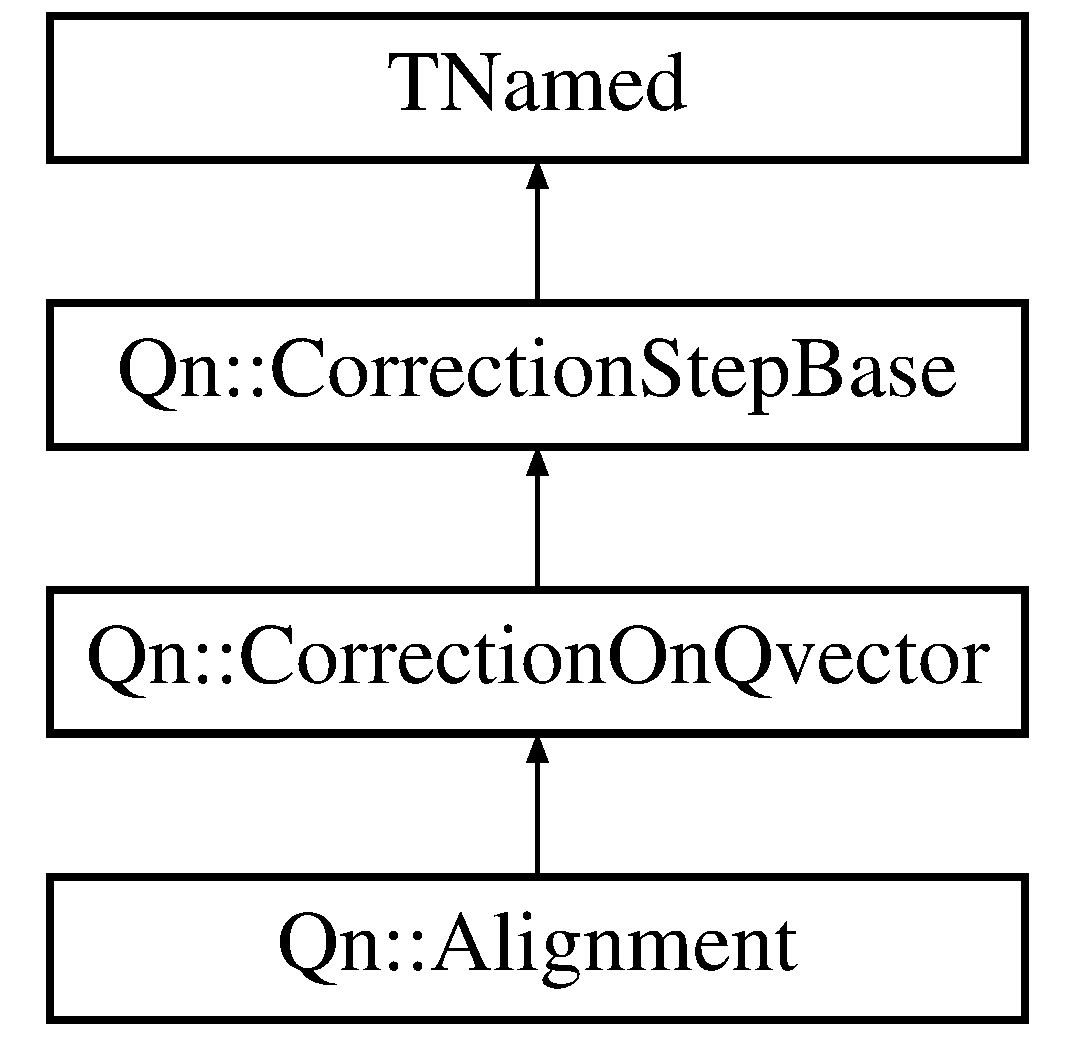
\includegraphics[height=4.000000cm]{classQn_1_1Alignment}
\end{center}
\end{figure}
\subsection*{Public Member Functions}
\begin{DoxyCompactItemize}
\item 
\mbox{\hyperlink{classQn_1_1Alignment_aeeec4b4eac91478f48d89e453cb3e10a}{Alignment}} ()
\item 
\mbox{\hyperlink{classQn_1_1Alignment_ad364189f6410b258123d7bd9d8bf0373}{$\sim$\+Alignment}} ()
\item 
void \mbox{\hyperlink{classQn_1_1Alignment_ae8e25ee857f8773757ba3936a8da9b70}{Set\+Harmonic\+Number\+For\+Alignment}} (Int\+\_\+t harmonic)
\item 
void \mbox{\hyperlink{classQn_1_1Alignment_a03d25738c83b68757e23eabc563d60c6}{Set\+Reference\+Configuration\+For\+Alignment}} (const char $\ast$name)
\item 
void \mbox{\hyperlink{classQn_1_1Alignment_a70d38db6adb97c47746d00f28f2b605c}{Set\+No\+Of\+Entries\+Threshold}} (Int\+\_\+t n\+No\+Of\+Entries)
\item 
virtual void \mbox{\hyperlink{classQn_1_1Alignment_ad9791cc06c9a7d8c407e1f783c7625f8}{Attached\+To\+Framework\+Manager}} ()
\item 
virtual Bool\+\_\+t \mbox{\hyperlink{classQn_1_1Alignment_a3ae85e6706fe2a04098d339fcfff9113}{Attach\+Input}} (T\+List $\ast$list)
\item 
virtual void \mbox{\hyperlink{classQn_1_1Alignment_a38007827bb028b2f2e0b4a3fb988d8ed}{After\+Inputs\+Attach\+Actions}} ()
\item 
virtual void \mbox{\hyperlink{classQn_1_1Alignment_afb0137bb2443eb44448bf15734096765}{Create\+Support\+Data\+Structures}} ()
\item 
virtual Bool\+\_\+t \mbox{\hyperlink{classQn_1_1Alignment_ada53d00555fc8a59644b3db5a8584de3}{Create\+Support\+Histograms}} (T\+List $\ast$list)
\item 
virtual Bool\+\_\+t \mbox{\hyperlink{classQn_1_1Alignment_a1b2499a48a748c4064804e0a5a283272}{Create\+Q\+A\+Histograms}} (T\+List $\ast$list)
\item 
virtual Bool\+\_\+t \mbox{\hyperlink{classQn_1_1Alignment_ac11ae0ae7f1ea1e1b8408d73469d54d1}{Create\+Nve\+Q\+A\+Histograms}} (T\+List $\ast$list)
\item 
virtual Bool\+\_\+t \mbox{\hyperlink{classQn_1_1Alignment_a57b815d9ce4d0ae4f94ff6cb46eb2514}{Process\+Corrections}} (const double $\ast$variable\+Container)
\item 
virtual Bool\+\_\+t \mbox{\hyperlink{classQn_1_1Alignment_af071fa4f51958ecfec6e6c58a7d84c84}{Process\+Data\+Collection}} (const double $\ast$variable\+Container)
\item 
\mbox{\Hypertarget{classQn_1_1Alignment_aba2ba181fbf1572b646ed0d225cb773b}\label{classQn_1_1Alignment_aba2ba181fbf1572b646ed0d225cb773b}} 
virtual void \mbox{\hyperlink{classQn_1_1Alignment_aba2ba181fbf1572b646ed0d225cb773b}{Clear\+Correction\+Step}} ()
\begin{DoxyCompactList}\small\item\em Clean the correction to accept a new event. \end{DoxyCompactList}\item 
virtual Bool\+\_\+t \mbox{\hyperlink{classQn_1_1Alignment_aaa38151d72ebf1aa97247ba07c4d16e5}{Is\+Being\+Applied}} () const
\item 
virtual Bool\+\_\+t \mbox{\hyperlink{classQn_1_1Alignment_af8ef33833778e9af4bdb7b82f679c941}{Report\+Usage}} (T\+List $\ast$calibration\+List, T\+List $\ast$apply\+List)
\end{DoxyCompactItemize}
\subsection*{Additional Inherited Members}


\subsection{Constructor \& Destructor Documentation}
\mbox{\Hypertarget{classQn_1_1Alignment_aeeec4b4eac91478f48d89e453cb3e10a}\label{classQn_1_1Alignment_aeeec4b4eac91478f48d89e453cb3e10a}} 
\index{Qn\+::\+Alignment@{Qn\+::\+Alignment}!Alignment@{Alignment}}
\index{Alignment@{Alignment}!Qn\+::\+Alignment@{Qn\+::\+Alignment}}
\subsubsection{\texorpdfstring{Alignment()}{Alignment()}}
{\footnotesize\ttfamily Qn\+::\+Alignment\+::\+Alignment (\begin{DoxyParamCaption}{ }\end{DoxyParamCaption})}

Default constructor Passes to the base class the identity data for the recentering and width equalization correction step \mbox{\Hypertarget{classQn_1_1Alignment_ad364189f6410b258123d7bd9d8bf0373}\label{classQn_1_1Alignment_ad364189f6410b258123d7bd9d8bf0373}} 
\index{Qn\+::\+Alignment@{Qn\+::\+Alignment}!````~Alignment@{$\sim$\+Alignment}}
\index{````~Alignment@{$\sim$\+Alignment}!Qn\+::\+Alignment@{Qn\+::\+Alignment}}
\subsubsection{\texorpdfstring{$\sim$\+Alignment()}{~Alignment()}}
{\footnotesize\ttfamily Qn\+::\+Alignment\+::$\sim$\+Alignment (\begin{DoxyParamCaption}{ }\end{DoxyParamCaption})}

Default destructor Releases the memory taken 

\subsection{Member Function Documentation}
\mbox{\Hypertarget{classQn_1_1Alignment_a38007827bb028b2f2e0b4a3fb988d8ed}\label{classQn_1_1Alignment_a38007827bb028b2f2e0b4a3fb988d8ed}} 
\index{Qn\+::\+Alignment@{Qn\+::\+Alignment}!After\+Inputs\+Attach\+Actions@{After\+Inputs\+Attach\+Actions}}
\index{After\+Inputs\+Attach\+Actions@{After\+Inputs\+Attach\+Actions}!Qn\+::\+Alignment@{Qn\+::\+Alignment}}
\subsubsection{\texorpdfstring{After\+Inputs\+Attach\+Actions()}{AfterInputsAttachActions()}}
{\footnotesize\ttfamily virtual void Qn\+::\+Alignment\+::\+After\+Inputs\+Attach\+Actions (\begin{DoxyParamCaption}{ }\end{DoxyParamCaption})\hspace{0.3cm}{\ttfamily [inline]}, {\ttfamily [virtual]}}

Perform after calibration histograms attach actions It is used to inform the different correction step that all conditions for running the network are in place so it is time to check if their requirements are satisfied

Does nothing for the time being 

Implements \mbox{\hyperlink{classQn_1_1CorrectionOnQvector_afa95ec7804ade8097d92002e0ea05e44}{Qn\+::\+Correction\+On\+Qvector}}.

\mbox{\Hypertarget{classQn_1_1Alignment_ad9791cc06c9a7d8c407e1f783c7625f8}\label{classQn_1_1Alignment_ad9791cc06c9a7d8c407e1f783c7625f8}} 
\index{Qn\+::\+Alignment@{Qn\+::\+Alignment}!Attached\+To\+Framework\+Manager@{Attached\+To\+Framework\+Manager}}
\index{Attached\+To\+Framework\+Manager@{Attached\+To\+Framework\+Manager}!Qn\+::\+Alignment@{Qn\+::\+Alignment}}
\subsubsection{\texorpdfstring{Attached\+To\+Framework\+Manager()}{AttachedToFrameworkManager()}}
{\footnotesize\ttfamily void Qn\+::\+Alignment\+::\+Attached\+To\+Framework\+Manager (\begin{DoxyParamCaption}{ }\end{DoxyParamCaption})\hspace{0.3cm}{\ttfamily [virtual]}}

Informs when the detector configuration has been attached to the framework manager Basically this allows interaction between the different framework sections at configuration time 

Implements \mbox{\hyperlink{classQn_1_1CorrectionOnQvector_ad2d37eb35973c854c7ffa3560a97d510}{Qn\+::\+Correction\+On\+Qvector}}.

\mbox{\Hypertarget{classQn_1_1Alignment_a3ae85e6706fe2a04098d339fcfff9113}\label{classQn_1_1Alignment_a3ae85e6706fe2a04098d339fcfff9113}} 
\index{Qn\+::\+Alignment@{Qn\+::\+Alignment}!Attach\+Input@{Attach\+Input}}
\index{Attach\+Input@{Attach\+Input}!Qn\+::\+Alignment@{Qn\+::\+Alignment}}
\subsubsection{\texorpdfstring{Attach\+Input()}{AttachInput()}}
{\footnotesize\ttfamily Bool\+\_\+t Qn\+::\+Alignment\+::\+Attach\+Input (\begin{DoxyParamCaption}\item[{T\+List $\ast$}]{list }\end{DoxyParamCaption})\hspace{0.3cm}{\ttfamily [virtual]}}

Attaches the needed input information to the correction step 
\begin{DoxyParams}{Parameters}
{\em list} & list where the inputs should be found \\
\hline
\end{DoxyParams}
\begin{DoxyReturn}{Returns}
k\+T\+R\+UE if everything went OK 
\end{DoxyReturn}


Implements \mbox{\hyperlink{classQn_1_1CorrectionOnQvector_acb7165c2eb071517fa977484bee7e445}{Qn\+::\+Correction\+On\+Qvector}}.

\mbox{\Hypertarget{classQn_1_1Alignment_ac11ae0ae7f1ea1e1b8408d73469d54d1}\label{classQn_1_1Alignment_ac11ae0ae7f1ea1e1b8408d73469d54d1}} 
\index{Qn\+::\+Alignment@{Qn\+::\+Alignment}!Create\+Nve\+Q\+A\+Histograms@{Create\+Nve\+Q\+A\+Histograms}}
\index{Create\+Nve\+Q\+A\+Histograms@{Create\+Nve\+Q\+A\+Histograms}!Qn\+::\+Alignment@{Qn\+::\+Alignment}}
\subsubsection{\texorpdfstring{Create\+Nve\+Q\+A\+Histograms()}{CreateNveQAHistograms()}}
{\footnotesize\ttfamily Bool\+\_\+t Qn\+::\+Alignment\+::\+Create\+Nve\+Q\+A\+Histograms (\begin{DoxyParamCaption}\item[{T\+List $\ast$}]{list }\end{DoxyParamCaption})\hspace{0.3cm}{\ttfamily [virtual]}}

Asks for non validated entries QA histograms creation

Allocates the histogram objects and creates the non validated entries QA histograms. 
\begin{DoxyParams}{Parameters}
{\em list} & list where the histograms should be incorporated for its persistence \\
\hline
\end{DoxyParams}
\begin{DoxyReturn}{Returns}
k\+T\+R\+UE if everything went OK 
\end{DoxyReturn}


Implements \mbox{\hyperlink{classQn_1_1CorrectionStepBase_acb488e715005f027e39c21ae5f4684da}{Qn\+::\+Correction\+Step\+Base}}.

\mbox{\Hypertarget{classQn_1_1Alignment_a1b2499a48a748c4064804e0a5a283272}\label{classQn_1_1Alignment_a1b2499a48a748c4064804e0a5a283272}} 
\index{Qn\+::\+Alignment@{Qn\+::\+Alignment}!Create\+Q\+A\+Histograms@{Create\+Q\+A\+Histograms}}
\index{Create\+Q\+A\+Histograms@{Create\+Q\+A\+Histograms}!Qn\+::\+Alignment@{Qn\+::\+Alignment}}
\subsubsection{\texorpdfstring{Create\+Q\+A\+Histograms()}{CreateQAHistograms()}}
{\footnotesize\ttfamily Bool\+\_\+t Qn\+::\+Alignment\+::\+Create\+Q\+A\+Histograms (\begin{DoxyParamCaption}\item[{T\+List $\ast$}]{list }\end{DoxyParamCaption})\hspace{0.3cm}{\ttfamily [virtual]}}

Asks for QA histograms creation

Allocates the histogram objects and creates the QA histograms. 
\begin{DoxyParams}{Parameters}
{\em list} & list where the histograms should be incorporated for its persistence \\
\hline
\end{DoxyParams}
\begin{DoxyReturn}{Returns}
k\+T\+R\+UE if everything went OK 
\end{DoxyReturn}


Implements \mbox{\hyperlink{classQn_1_1CorrectionStepBase_a21f58f5d91209c1c74d0928cf0b3e26d}{Qn\+::\+Correction\+Step\+Base}}.

\mbox{\Hypertarget{classQn_1_1Alignment_afb0137bb2443eb44448bf15734096765}\label{classQn_1_1Alignment_afb0137bb2443eb44448bf15734096765}} 
\index{Qn\+::\+Alignment@{Qn\+::\+Alignment}!Create\+Support\+Data\+Structures@{Create\+Support\+Data\+Structures}}
\index{Create\+Support\+Data\+Structures@{Create\+Support\+Data\+Structures}!Qn\+::\+Alignment@{Qn\+::\+Alignment}}
\subsubsection{\texorpdfstring{Create\+Support\+Data\+Structures()}{CreateSupportDataStructures()}}
{\footnotesize\ttfamily void Qn\+::\+Alignment\+::\+Create\+Support\+Data\+Structures (\begin{DoxyParamCaption}{ }\end{DoxyParamCaption})\hspace{0.3cm}{\ttfamily [virtual]}}

Asks for support data structures creation

Locates the reference detector configuration for alignment if its name has been previously stored Creates the recentered \mbox{\hyperlink{namespaceQn}{Qn}} vector 

Implements \mbox{\hyperlink{classQn_1_1CorrectionOnQvector_ac7c019bc36ac90618ed6e5fc768ca593}{Qn\+::\+Correction\+On\+Qvector}}.

\mbox{\Hypertarget{classQn_1_1Alignment_ada53d00555fc8a59644b3db5a8584de3}\label{classQn_1_1Alignment_ada53d00555fc8a59644b3db5a8584de3}} 
\index{Qn\+::\+Alignment@{Qn\+::\+Alignment}!Create\+Support\+Histograms@{Create\+Support\+Histograms}}
\index{Create\+Support\+Histograms@{Create\+Support\+Histograms}!Qn\+::\+Alignment@{Qn\+::\+Alignment}}
\subsubsection{\texorpdfstring{Create\+Support\+Histograms()}{CreateSupportHistograms()}}
{\footnotesize\ttfamily Bool\+\_\+t Qn\+::\+Alignment\+::\+Create\+Support\+Histograms (\begin{DoxyParamCaption}\item[{T\+List $\ast$}]{list }\end{DoxyParamCaption})\hspace{0.3cm}{\ttfamily [virtual]}}

Asks for support histograms creation

Allocates the histogram objects and creates the calibration histograms.

Process concurrency requires Calibration Histograms creation for all concurrent processes but not for Input Histograms so, we delete previously allocated ones. 
\begin{DoxyParams}{Parameters}
{\em list} & list where the histograms should be incorporated for its persistence \\
\hline
\end{DoxyParams}
\begin{DoxyReturn}{Returns}
k\+T\+R\+UE if everything went OK 
\end{DoxyReturn}


Implements \mbox{\hyperlink{classQn_1_1CorrectionOnQvector_addcdd98787c99ea34a2511be2cdc8de4}{Qn\+::\+Correction\+On\+Qvector}}.

\mbox{\Hypertarget{classQn_1_1Alignment_aaa38151d72ebf1aa97247ba07c4d16e5}\label{classQn_1_1Alignment_aaa38151d72ebf1aa97247ba07c4d16e5}} 
\index{Qn\+::\+Alignment@{Qn\+::\+Alignment}!Is\+Being\+Applied@{Is\+Being\+Applied}}
\index{Is\+Being\+Applied@{Is\+Being\+Applied}!Qn\+::\+Alignment@{Qn\+::\+Alignment}}
\subsubsection{\texorpdfstring{Is\+Being\+Applied()}{IsBeingApplied()}}
{\footnotesize\ttfamily Bool\+\_\+t Qn\+::\+Alignment\+::\+Is\+Being\+Applied (\begin{DoxyParamCaption}{ }\end{DoxyParamCaption}) const\hspace{0.3cm}{\ttfamily [virtual]}}

Reports if the correction step is being applied Returns T\+R\+UE if in the proper state for applying the correction step \begin{DoxyReturn}{Returns}
T\+R\+UE if the correction step is being applied 
\end{DoxyReturn}


Implements \mbox{\hyperlink{classQn_1_1CorrectionOnQvector_a4d47a1c241b4bfd5ac98d6fdbc90eb79}{Qn\+::\+Correction\+On\+Qvector}}.

\mbox{\Hypertarget{classQn_1_1Alignment_a57b815d9ce4d0ae4f94ff6cb46eb2514}\label{classQn_1_1Alignment_a57b815d9ce4d0ae4f94ff6cb46eb2514}} 
\index{Qn\+::\+Alignment@{Qn\+::\+Alignment}!Process\+Corrections@{Process\+Corrections}}
\index{Process\+Corrections@{Process\+Corrections}!Qn\+::\+Alignment@{Qn\+::\+Alignment}}
\subsubsection{\texorpdfstring{Process\+Corrections()}{ProcessCorrections()}}
{\footnotesize\ttfamily Bool\+\_\+t Qn\+::\+Alignment\+::\+Process\+Corrections (\begin{DoxyParamCaption}\item[{const double $\ast$}]{variable\+Container }\end{DoxyParamCaption})\hspace{0.3cm}{\ttfamily [virtual]}}

Processes the correction step

Apply the correction step \begin{DoxyReturn}{Returns}
k\+T\+R\+UE if the correction step was applied 
\end{DoxyReturn}


Implements \mbox{\hyperlink{classQn_1_1CorrectionOnQvector_a2c2d7f0e48471fb9269f0b5f9aa3e836}{Qn\+::\+Correction\+On\+Qvector}}.

\mbox{\Hypertarget{classQn_1_1Alignment_af071fa4f51958ecfec6e6c58a7d84c84}\label{classQn_1_1Alignment_af071fa4f51958ecfec6e6c58a7d84c84}} 
\index{Qn\+::\+Alignment@{Qn\+::\+Alignment}!Process\+Data\+Collection@{Process\+Data\+Collection}}
\index{Process\+Data\+Collection@{Process\+Data\+Collection}!Qn\+::\+Alignment@{Qn\+::\+Alignment}}
\subsubsection{\texorpdfstring{Process\+Data\+Collection()}{ProcessDataCollection()}}
{\footnotesize\ttfamily Bool\+\_\+t Qn\+::\+Alignment\+::\+Process\+Data\+Collection (\begin{DoxyParamCaption}\item[{const double $\ast$}]{variable\+Container }\end{DoxyParamCaption})\hspace{0.3cm}{\ttfamily [virtual]}}

Processes the correction step data collection

Collect data for the correction step. \begin{DoxyReturn}{Returns}
k\+T\+R\+UE if the correction step was applied 
\end{DoxyReturn}


Implements \mbox{\hyperlink{classQn_1_1CorrectionOnQvector_a2c0a668d885b5a42503869303c859a0b}{Qn\+::\+Correction\+On\+Qvector}}.

\mbox{\Hypertarget{classQn_1_1Alignment_af8ef33833778e9af4bdb7b82f679c941}\label{classQn_1_1Alignment_af8ef33833778e9af4bdb7b82f679c941}} 
\index{Qn\+::\+Alignment@{Qn\+::\+Alignment}!Report\+Usage@{Report\+Usage}}
\index{Report\+Usage@{Report\+Usage}!Qn\+::\+Alignment@{Qn\+::\+Alignment}}
\subsubsection{\texorpdfstring{Report\+Usage()}{ReportUsage()}}
{\footnotesize\ttfamily Bool\+\_\+t Qn\+::\+Alignment\+::\+Report\+Usage (\begin{DoxyParamCaption}\item[{T\+List $\ast$}]{calibration\+List,  }\item[{T\+List $\ast$}]{apply\+List }\end{DoxyParamCaption})\hspace{0.3cm}{\ttfamily [virtual]}}

Report on correction usage Correction step should incorporate its name in calibration list if it is producing information calibration in the ongoing step and in the apply list if it is applying correction in the ongoing step. 
\begin{DoxyParams}{Parameters}
{\em calibration\+List} & list containing the correction steps producing calibration information \\
\hline
{\em apply\+List} & list containing the correction steps applying corrections \\
\hline
\end{DoxyParams}
\begin{DoxyReturn}{Returns}
k\+T\+R\+UE if the correction step is being applied 
\end{DoxyReturn}


Implements \mbox{\hyperlink{classQn_1_1CorrectionOnQvector_a322860c299f0ca1db46ddd57c0828ba1}{Qn\+::\+Correction\+On\+Qvector}}.

\mbox{\Hypertarget{classQn_1_1Alignment_ae8e25ee857f8773757ba3936a8da9b70}\label{classQn_1_1Alignment_ae8e25ee857f8773757ba3936a8da9b70}} 
\index{Qn\+::\+Alignment@{Qn\+::\+Alignment}!Set\+Harmonic\+Number\+For\+Alignment@{Set\+Harmonic\+Number\+For\+Alignment}}
\index{Set\+Harmonic\+Number\+For\+Alignment@{Set\+Harmonic\+Number\+For\+Alignment}!Qn\+::\+Alignment@{Qn\+::\+Alignment}}
\subsubsection{\texorpdfstring{Set\+Harmonic\+Number\+For\+Alignment()}{SetHarmonicNumberForAlignment()}}
{\footnotesize\ttfamily void Qn\+::\+Alignment\+::\+Set\+Harmonic\+Number\+For\+Alignment (\begin{DoxyParamCaption}\item[{Int\+\_\+t}]{harmonic }\end{DoxyParamCaption})\hspace{0.3cm}{\ttfamily [inline]}}

Set the harmonic number used for alignment 
\begin{DoxyParams}{Parameters}
{\em harmonic} & harmonic number \\
\hline
\end{DoxyParams}
\mbox{\Hypertarget{classQn_1_1Alignment_a70d38db6adb97c47746d00f28f2b605c}\label{classQn_1_1Alignment_a70d38db6adb97c47746d00f28f2b605c}} 
\index{Qn\+::\+Alignment@{Qn\+::\+Alignment}!Set\+No\+Of\+Entries\+Threshold@{Set\+No\+Of\+Entries\+Threshold}}
\index{Set\+No\+Of\+Entries\+Threshold@{Set\+No\+Of\+Entries\+Threshold}!Qn\+::\+Alignment@{Qn\+::\+Alignment}}
\subsubsection{\texorpdfstring{Set\+No\+Of\+Entries\+Threshold()}{SetNoOfEntriesThreshold()}}
{\footnotesize\ttfamily void Qn\+::\+Alignment\+::\+Set\+No\+Of\+Entries\+Threshold (\begin{DoxyParamCaption}\item[{Int\+\_\+t}]{n\+No\+Of\+Entries }\end{DoxyParamCaption})\hspace{0.3cm}{\ttfamily [inline]}}

Set the minimum number of entries for calibration histogram bin content validation 
\begin{DoxyParams}{Parameters}
{\em n\+No\+Of\+Entries} & the number of entries threshold \\
\hline
\end{DoxyParams}
\mbox{\Hypertarget{classQn_1_1Alignment_a03d25738c83b68757e23eabc563d60c6}\label{classQn_1_1Alignment_a03d25738c83b68757e23eabc563d60c6}} 
\index{Qn\+::\+Alignment@{Qn\+::\+Alignment}!Set\+Reference\+Configuration\+For\+Alignment@{Set\+Reference\+Configuration\+For\+Alignment}}
\index{Set\+Reference\+Configuration\+For\+Alignment@{Set\+Reference\+Configuration\+For\+Alignment}!Qn\+::\+Alignment@{Qn\+::\+Alignment}}
\subsubsection{\texorpdfstring{Set\+Reference\+Configuration\+For\+Alignment()}{SetReferenceConfigurationForAlignment()}}
{\footnotesize\ttfamily void Qn\+::\+Alignment\+::\+Set\+Reference\+Configuration\+For\+Alignment (\begin{DoxyParamCaption}\item[{const char $\ast$}]{name }\end{DoxyParamCaption})}

Set the detector configuration used as reference for alignment The detector configuration name is stored for further use. 
\begin{DoxyParams}{Parameters}
{\em name} & the name of the reference detector configuration \\
\hline
\end{DoxyParams}


The documentation for this class was generated from the following files\+:\begin{DoxyCompactItemize}
\item 
D\+T\+\_\+\+Flow/\+Qn\+Corrections/include/Alignment.\+h\item 
D\+T\+\_\+\+Flow/\+Qn\+Corrections/Alignment.\+cpp\end{DoxyCompactItemize}

\hypertarget{classQn_1_1Axis}{}\section{Qn\+:\+:Axis Class Reference}
\label{classQn_1_1Axis}\index{Qn\+::\+Axis@{Qn\+::\+Axis}}


Parameter axis with variable bin widths.  




{\ttfamily \#include $<$Axis.\+h$>$}

\subsection*{Public Types}
\begin{DoxyCompactItemize}
\item 
\mbox{\Hypertarget{classQn_1_1Axis_aecaef827e021f557908269e846ec953f}\label{classQn_1_1Axis_aecaef827e021f557908269e846ec953f}} 
typedef std\+::vector$<$ float $>$\+::const\+\_\+iterator {\bfseries citerator}
\item 
\mbox{\Hypertarget{classQn_1_1Axis_a17ec979786a378efeb648d11be4ddbc2}\label{classQn_1_1Axis_a17ec979786a378efeb648d11be4ddbc2}} 
typedef std\+::vector$<$ float $>$\+::iterator {\bfseries iterator}
\end{DoxyCompactItemize}
\subsection*{Public Member Functions}
\begin{DoxyCompactItemize}
\item 
\mbox{\Hypertarget{classQn_1_1Axis_afda68534099c45ff3e4105a9dd5d6f15}\label{classQn_1_1Axis_afda68534099c45ff3e4105a9dd5d6f15}} 
\mbox{\hyperlink{classQn_1_1Axis_afda68534099c45ff3e4105a9dd5d6f15}{Axis}} ()=default
\begin{DoxyCompactList}\small\item\em default constructor \end{DoxyCompactList}\item 
\mbox{\Hypertarget{classQn_1_1Axis_a681cf1e062f2256bcdaea4c990b87e79}\label{classQn_1_1Axis_a681cf1e062f2256bcdaea4c990b87e79}} 
virtual \mbox{\hyperlink{classQn_1_1Axis_a681cf1e062f2256bcdaea4c990b87e79}{$\sim$\+Axis}} ()=default
\begin{DoxyCompactList}\small\item\em default destructor \end{DoxyCompactList}\item 
\mbox{\hyperlink{classQn_1_1Axis_aecffcf8ea49a172d67e5a620082f3914}{Axis}} (std\+::string name, std\+::vector$<$ float $>$ bin\+\_\+edges)
\item 
\mbox{\hyperlink{classQn_1_1Axis_aba5f6d07ac72fc4eda097edd15336c86}{Axis}} (std\+::string name, const int nbins, const float lowbin, const float upbin)
\item 
\mbox{\Hypertarget{classQn_1_1Axis_a5a1bb456f84f482991c75154ca8dbe2c}\label{classQn_1_1Axis_a5a1bb456f84f482991c75154ca8dbe2c}} 
{\bfseries Axis} (const \mbox{\hyperlink{classQn_1_1Axis}{Qn\+::\+Axis}} \&axis)
\item 
\mbox{\Hypertarget{classQn_1_1Axis_acf2d80052d44ddb91ac2223747ebd8ab}\label{classQn_1_1Axis_acf2d80052d44ddb91ac2223747ebd8ab}} 
bool {\bfseries operator==} (const \mbox{\hyperlink{classQn_1_1Axis}{Axis}} \&axis) const
\item 
\mbox{\Hypertarget{classQn_1_1Axis_a1b3db6cf7a0918edc640a8a38556a04a}\label{classQn_1_1Axis_a1b3db6cf7a0918edc640a8a38556a04a}} 
citerator \mbox{\hyperlink{classQn_1_1Axis_a1b3db6cf7a0918edc640a8a38556a04a}{begin}} () const
\begin{DoxyCompactList}\small\item\em iterator for external use \end{DoxyCompactList}\item 
\mbox{\Hypertarget{classQn_1_1Axis_a41d685ea3eb8ed0b3b0cf91228caf819}\label{classQn_1_1Axis_a41d685ea3eb8ed0b3b0cf91228caf819}} 
citerator \mbox{\hyperlink{classQn_1_1Axis_a41d685ea3eb8ed0b3b0cf91228caf819}{end}} () const
\begin{DoxyCompactList}\small\item\em iterator for external use \end{DoxyCompactList}\item 
\mbox{\Hypertarget{classQn_1_1Axis_a46c31b76eb3c41e25c75c8e540d2d037}\label{classQn_1_1Axis_a46c31b76eb3c41e25c75c8e540d2d037}} 
iterator \mbox{\hyperlink{classQn_1_1Axis_a46c31b76eb3c41e25c75c8e540d2d037}{begin}} ()
\begin{DoxyCompactList}\small\item\em iterator for external use \end{DoxyCompactList}\item 
\mbox{\Hypertarget{classQn_1_1Axis_a4d2e34076f1915409a8dae58cce1812f}\label{classQn_1_1Axis_a4d2e34076f1915409a8dae58cce1812f}} 
iterator \mbox{\hyperlink{classQn_1_1Axis_a4d2e34076f1915409a8dae58cce1812f}{end}} ()
\begin{DoxyCompactList}\small\item\em iterator for external use \end{DoxyCompactList}\item 
void \mbox{\hyperlink{classQn_1_1Axis_a80eca8411e7749624fbd146248869fc8}{Set\+Name}} (const std\+::string name)
\item 
std\+::string \mbox{\hyperlink{classQn_1_1Axis_a355ae8809138b8b1017d51d607059ea6}{Name}} () const
\item 
long \mbox{\hyperlink{classQn_1_1Axis_ae2a512dfaf15fbeddfa02c85adb9883f}{Find\+Bin}} (const float value) const
\item 
\mbox{\Hypertarget{classQn_1_1Axis_af39b2ee7c9ad0bff5bd7069d6b4f3288}\label{classQn_1_1Axis_af39b2ee7c9ad0bff5bd7069d6b4f3288}} 
std\+::string {\bfseries Get\+Bin\+Name} (unsigned int i) const
\item 
citerator \mbox{\hyperlink{classQn_1_1Axis_a757b881b8615df4ed6d6ba917770b354}{Find\+Bin\+Iter}} (const float value)
\item 
std\+::vector$<$ float $>$\+::size\+\_\+type \mbox{\hyperlink{classQn_1_1Axis_ac3db40c16950698d698f55bcb1c51bf9}{size}} () const
\item 
float \mbox{\hyperlink{classQn_1_1Axis_ac40575006fde015d3b25c7e838e21994}{Get\+Lower\+Bin\+Edge}} (const unsigned long bin) const
\item 
float \mbox{\hyperlink{classQn_1_1Axis_a8ac94e3567fb894439c0a4844c62e4a2}{Get\+Upper\+Bin\+Edge}} (const unsigned long bin) const
\item 
float \mbox{\hyperlink{classQn_1_1Axis_ae9c911292458f9668e689be50614d8dc}{Get\+First\+Bin\+Edge}} () const
\item 
float \mbox{\hyperlink{classQn_1_1Axis_ac363f1585fc08372b81ebba24f2cd38f}{Get\+Last\+Bin\+Edge}} () const
\end{DoxyCompactItemize}


\subsection{Detailed Description}
Parameter axis with variable bin widths. 

Basic axis implementation 

\subsection{Constructor \& Destructor Documentation}
\mbox{\Hypertarget{classQn_1_1Axis_aecffcf8ea49a172d67e5a620082f3914}\label{classQn_1_1Axis_aecffcf8ea49a172d67e5a620082f3914}} 
\index{Qn\+::\+Axis@{Qn\+::\+Axis}!Axis@{Axis}}
\index{Axis@{Axis}!Qn\+::\+Axis@{Qn\+::\+Axis}}
\subsubsection{\texorpdfstring{Axis()}{Axis()}\hspace{0.1cm}{\footnotesize\ttfamily [1/2]}}
{\footnotesize\ttfamily Qn\+::\+Axis\+::\+Axis (\begin{DoxyParamCaption}\item[{std\+::string}]{name,  }\item[{std\+::vector$<$ float $>$}]{bin\+\_\+edges }\end{DoxyParamCaption})\hspace{0.3cm}{\ttfamily [inline]}}

Constructor for variable or fixed bin width. 
\begin{DoxyParams}{Parameters}
{\em name} & name of axis. \\
\hline
{\em bin\+\_\+edges} & vector of bin edges. starting with lowest bin edge and ending with uppermost bin edge. \\
\hline
\end{DoxyParams}
\mbox{\Hypertarget{classQn_1_1Axis_aba5f6d07ac72fc4eda097edd15336c86}\label{classQn_1_1Axis_aba5f6d07ac72fc4eda097edd15336c86}} 
\index{Qn\+::\+Axis@{Qn\+::\+Axis}!Axis@{Axis}}
\index{Axis@{Axis}!Qn\+::\+Axis@{Qn\+::\+Axis}}
\subsubsection{\texorpdfstring{Axis()}{Axis()}\hspace{0.1cm}{\footnotesize\ttfamily [2/2]}}
{\footnotesize\ttfamily Qn\+::\+Axis\+::\+Axis (\begin{DoxyParamCaption}\item[{std\+::string}]{name,  }\item[{const int}]{nbins,  }\item[{const float}]{lowbin,  }\item[{const float}]{upbin }\end{DoxyParamCaption})\hspace{0.3cm}{\ttfamily [inline]}}

Constructor for fixed bin width. Calculates bin width automatically and sets bin edges. 
\begin{DoxyParams}{Parameters}
{\em name} & name of axis \\
\hline
{\em nbins} & number of bins \\
\hline
{\em lowbin} & lowest bin edge \\
\hline
{\em upbin} & uppermost bin edge \\
\hline
\end{DoxyParams}


\subsection{Member Function Documentation}
\mbox{\Hypertarget{classQn_1_1Axis_ae2a512dfaf15fbeddfa02c85adb9883f}\label{classQn_1_1Axis_ae2a512dfaf15fbeddfa02c85adb9883f}} 
\index{Qn\+::\+Axis@{Qn\+::\+Axis}!Find\+Bin@{Find\+Bin}}
\index{Find\+Bin@{Find\+Bin}!Qn\+::\+Axis@{Qn\+::\+Axis}}
\subsubsection{\texorpdfstring{Find\+Bin()}{FindBin()}}
{\footnotesize\ttfamily long Qn\+::\+Axis\+::\+Find\+Bin (\begin{DoxyParamCaption}\item[{const float}]{value }\end{DoxyParamCaption}) const\hspace{0.3cm}{\ttfamily [inline]}}

Finds bin index for a given value if value is smaller than lowest bin return -\/1. 
\begin{DoxyParams}{Parameters}
{\em value} & for finding corresponding bin \\
\hline
\end{DoxyParams}
\begin{DoxyReturn}{Returns}
bin index 
\end{DoxyReturn}
\mbox{\Hypertarget{classQn_1_1Axis_a757b881b8615df4ed6d6ba917770b354}\label{classQn_1_1Axis_a757b881b8615df4ed6d6ba917770b354}} 
\index{Qn\+::\+Axis@{Qn\+::\+Axis}!Find\+Bin\+Iter@{Find\+Bin\+Iter}}
\index{Find\+Bin\+Iter@{Find\+Bin\+Iter}!Qn\+::\+Axis@{Qn\+::\+Axis}}
\subsubsection{\texorpdfstring{Find\+Bin\+Iter()}{FindBinIter()}}
{\footnotesize\ttfamily Qn\+::\+Axis\+::citerator Qn\+::\+Axis\+::\+Find\+Bin\+Iter (\begin{DoxyParamCaption}\item[{const float}]{value }\end{DoxyParamCaption})\hspace{0.3cm}{\ttfamily [inline]}}

Finds bin iterator for a given value if value is smaller than lowest bin returns \mbox{\hyperlink{classQn_1_1Axis_a4d2e34076f1915409a8dae58cce1812f}{end()}}. 
\begin{DoxyParams}{Parameters}
{\em value} & for finding corresponding bin \\
\hline
\end{DoxyParams}
\begin{DoxyReturn}{Returns}
bin index 
\end{DoxyReturn}
\mbox{\Hypertarget{classQn_1_1Axis_ae9c911292458f9668e689be50614d8dc}\label{classQn_1_1Axis_ae9c911292458f9668e689be50614d8dc}} 
\index{Qn\+::\+Axis@{Qn\+::\+Axis}!Get\+First\+Bin\+Edge@{Get\+First\+Bin\+Edge}}
\index{Get\+First\+Bin\+Edge@{Get\+First\+Bin\+Edge}!Qn\+::\+Axis@{Qn\+::\+Axis}}
\subsubsection{\texorpdfstring{Get\+First\+Bin\+Edge()}{GetFirstBinEdge()}}
{\footnotesize\ttfamily float Qn\+::\+Axis\+::\+Get\+First\+Bin\+Edge (\begin{DoxyParamCaption}{ }\end{DoxyParamCaption}) const\hspace{0.3cm}{\ttfamily [inline]}}

Gets lower bin edge 
\begin{DoxyParams}{Parameters}
{\em bin} & Index of bin of interest \\
\hline
\end{DoxyParams}
\begin{DoxyReturn}{Returns}
lower edge of bin of interest 
\end{DoxyReturn}
\mbox{\Hypertarget{classQn_1_1Axis_ac363f1585fc08372b81ebba24f2cd38f}\label{classQn_1_1Axis_ac363f1585fc08372b81ebba24f2cd38f}} 
\index{Qn\+::\+Axis@{Qn\+::\+Axis}!Get\+Last\+Bin\+Edge@{Get\+Last\+Bin\+Edge}}
\index{Get\+Last\+Bin\+Edge@{Get\+Last\+Bin\+Edge}!Qn\+::\+Axis@{Qn\+::\+Axis}}
\subsubsection{\texorpdfstring{Get\+Last\+Bin\+Edge()}{GetLastBinEdge()}}
{\footnotesize\ttfamily float Qn\+::\+Axis\+::\+Get\+Last\+Bin\+Edge (\begin{DoxyParamCaption}{ }\end{DoxyParamCaption}) const\hspace{0.3cm}{\ttfamily [inline]}}

Gets upper bin edge 
\begin{DoxyParams}{Parameters}
{\em bin} & Index of bin of interest \\
\hline
\end{DoxyParams}
\begin{DoxyReturn}{Returns}
upper edge of bin of interest 
\end{DoxyReturn}
\mbox{\Hypertarget{classQn_1_1Axis_ac40575006fde015d3b25c7e838e21994}\label{classQn_1_1Axis_ac40575006fde015d3b25c7e838e21994}} 
\index{Qn\+::\+Axis@{Qn\+::\+Axis}!Get\+Lower\+Bin\+Edge@{Get\+Lower\+Bin\+Edge}}
\index{Get\+Lower\+Bin\+Edge@{Get\+Lower\+Bin\+Edge}!Qn\+::\+Axis@{Qn\+::\+Axis}}
\subsubsection{\texorpdfstring{Get\+Lower\+Bin\+Edge()}{GetLowerBinEdge()}}
{\footnotesize\ttfamily float Qn\+::\+Axis\+::\+Get\+Lower\+Bin\+Edge (\begin{DoxyParamCaption}\item[{const unsigned long}]{bin }\end{DoxyParamCaption}) const\hspace{0.3cm}{\ttfamily [inline]}}

Gets lower bin edge 
\begin{DoxyParams}{Parameters}
{\em bin} & Index of bin of interest \\
\hline
\end{DoxyParams}
\begin{DoxyReturn}{Returns}
lower edge of bin of interest 
\end{DoxyReturn}
\mbox{\Hypertarget{classQn_1_1Axis_a8ac94e3567fb894439c0a4844c62e4a2}\label{classQn_1_1Axis_a8ac94e3567fb894439c0a4844c62e4a2}} 
\index{Qn\+::\+Axis@{Qn\+::\+Axis}!Get\+Upper\+Bin\+Edge@{Get\+Upper\+Bin\+Edge}}
\index{Get\+Upper\+Bin\+Edge@{Get\+Upper\+Bin\+Edge}!Qn\+::\+Axis@{Qn\+::\+Axis}}
\subsubsection{\texorpdfstring{Get\+Upper\+Bin\+Edge()}{GetUpperBinEdge()}}
{\footnotesize\ttfamily float Qn\+::\+Axis\+::\+Get\+Upper\+Bin\+Edge (\begin{DoxyParamCaption}\item[{const unsigned long}]{bin }\end{DoxyParamCaption}) const\hspace{0.3cm}{\ttfamily [inline]}}

Gets upper bin edge 
\begin{DoxyParams}{Parameters}
{\em bin} & Index of bin of interest \\
\hline
\end{DoxyParams}
\begin{DoxyReturn}{Returns}
upper edge of bin of interest 
\end{DoxyReturn}
\mbox{\Hypertarget{classQn_1_1Axis_a355ae8809138b8b1017d51d607059ea6}\label{classQn_1_1Axis_a355ae8809138b8b1017d51d607059ea6}} 
\index{Qn\+::\+Axis@{Qn\+::\+Axis}!Name@{Name}}
\index{Name@{Name}!Qn\+::\+Axis@{Qn\+::\+Axis}}
\subsubsection{\texorpdfstring{Name()}{Name()}}
{\footnotesize\ttfamily std\+::string Qn\+::\+Axis\+::\+Name (\begin{DoxyParamCaption}{ }\end{DoxyParamCaption}) const\hspace{0.3cm}{\ttfamily [inline]}}

Returns Name of axis. \begin{DoxyReturn}{Returns}
name of axis 
\end{DoxyReturn}
\mbox{\Hypertarget{classQn_1_1Axis_a80eca8411e7749624fbd146248869fc8}\label{classQn_1_1Axis_a80eca8411e7749624fbd146248869fc8}} 
\index{Qn\+::\+Axis@{Qn\+::\+Axis}!Set\+Name@{Set\+Name}}
\index{Set\+Name@{Set\+Name}!Qn\+::\+Axis@{Qn\+::\+Axis}}
\subsubsection{\texorpdfstring{Set\+Name()}{SetName()}}
{\footnotesize\ttfamily void Qn\+::\+Axis\+::\+Set\+Name (\begin{DoxyParamCaption}\item[{const std\+::string}]{name }\end{DoxyParamCaption})\hspace{0.3cm}{\ttfamily [inline]}}

Set Name of axis. 
\begin{DoxyParams}{Parameters}
{\em name} & name of axis \\
\hline
\end{DoxyParams}
\mbox{\Hypertarget{classQn_1_1Axis_ac3db40c16950698d698f55bcb1c51bf9}\label{classQn_1_1Axis_ac3db40c16950698d698f55bcb1c51bf9}} 
\index{Qn\+::\+Axis@{Qn\+::\+Axis}!size@{size}}
\index{size@{size}!Qn\+::\+Axis@{Qn\+::\+Axis}}
\subsubsection{\texorpdfstring{size()}{size()}}
{\footnotesize\ttfamily std\+::vector$<$float$>$\+::size\+\_\+type Qn\+::\+Axis\+::size (\begin{DoxyParamCaption}{ }\end{DoxyParamCaption}) const\hspace{0.3cm}{\ttfamily [inline]}}

Returns number of bins. \begin{DoxyReturn}{Returns}
number of bins. 
\end{DoxyReturn}


The documentation for this class was generated from the following files\+:\begin{DoxyCompactItemize}
\item 
D\+T\+\_\+\+Flow/\+Base/include/Axis.\+h\item 
D\+T\+\_\+\+Flow/\+Base/Axis.\+cpp\end{DoxyCompactItemize}

\hypertarget{classBase}{}\section{Base Class Reference}
\label{classBase}\index{Base@{Base}}


\subsection{Detailed Description}
a Detector 

The documentation for this class was generated from the following file\+:\begin{DoxyCompactItemize}
\item 
D\+T\+\_\+\+Flow/\+Correction/include/Detector.\+h\end{DoxyCompactItemize}

\hypertarget{classQn_1_1CorrectionCalculator}{}\section{Qn\+:\+:Correction\+Calculator Class Reference}
\label{classQn_1_1CorrectionCalculator}\index{Qn\+::\+Correction\+Calculator@{Qn\+::\+Correction\+Calculator}}
Inheritance diagram for Qn\+:\+:Correction\+Calculator\+:\begin{figure}[H]
\begin{center}
\leavevmode
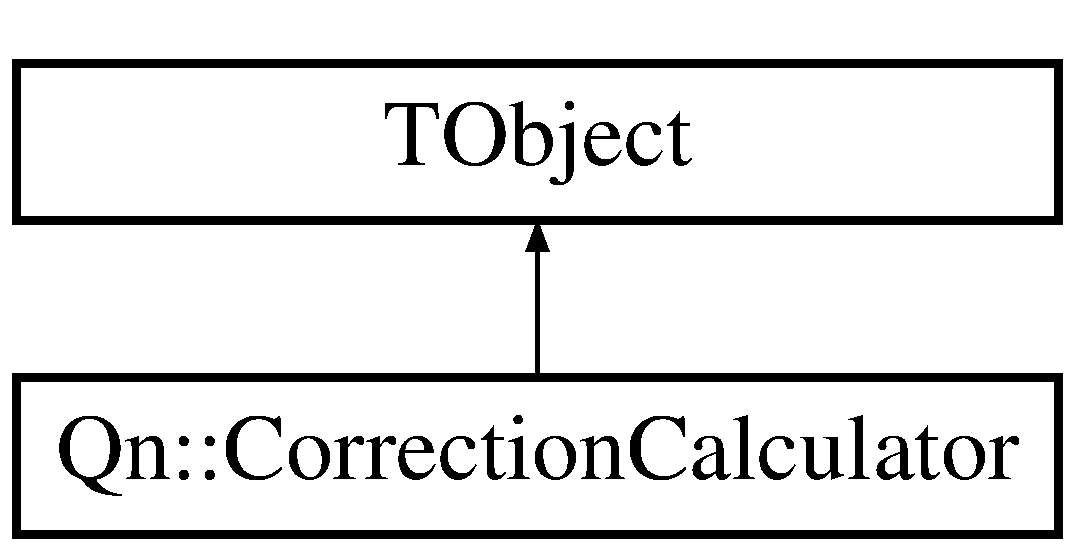
\includegraphics[height=2.000000cm]{classQn_1_1CorrectionCalculator}
\end{center}
\end{figure}
\subsection*{Public Member Functions}
\begin{DoxyCompactItemize}
\item 
\mbox{\hyperlink{classQn_1_1CorrectionCalculator_a66db1979cc23ca81e8cace68d816f8c3}{Correction\+Calculator}} ()
\item 
virtual \mbox{\hyperlink{classQn_1_1CorrectionCalculator_a52d30901588086ead7400efffcc56c98}{$\sim$\+Correction\+Calculator}} ()
\item 
void \mbox{\hyperlink{classQn_1_1CorrectionCalculator_ac0ad939e7fbdcb80c6b2ee08fc7d3447}{Set\+List\+Of\+Processes\+Names}} (T\+Obj\+Array $\ast$names)
\item 
void \mbox{\hyperlink{classQn_1_1CorrectionCalculator_a74c96c14696e8221ec839d7c8b5f773b}{Set\+Current\+Process\+List\+Name}} (const char $\ast$name)
\item 
void \mbox{\hyperlink{classQn_1_1CorrectionCalculator_a62057548ca452e31e76ff98c9e5b6fd0}{Set\+Calibration\+Histograms\+List}} (T\+File $\ast$calibration\+File)
\item 
void \mbox{\hyperlink{classQn_1_1CorrectionCalculator_a00dfda0d66bfdeeec6497580e491774a}{Set\+Should\+Fill\+Output\+Histograms}} (Bool\+\_\+t enable=k\+T\+R\+UE)
\item 
void \mbox{\hyperlink{classQn_1_1CorrectionCalculator_a598ddf62e8f05b71bf3e5c573a4af6c2}{Set\+Should\+Fill\+Q\+A\+Histograms}} (Bool\+\_\+t enable=k\+T\+R\+UE)
\item 
void \mbox{\hyperlink{classQn_1_1CorrectionCalculator_a97f032c649755a11b88f919dbb02c717}{Set\+Should\+Fill\+Nve\+Q\+A\+Histograms}} (Bool\+\_\+t enable=k\+T\+R\+UE)
\item 
void \mbox{\hyperlink{classQn_1_1CorrectionCalculator_abfa3d7424b677f225d2e7c4f37d70e8a}{Set\+Should\+Fill\+Qn\+Vector\+Tree}} (Bool\+\_\+t enable=k\+T\+R\+UE)
\item 
void \mbox{\hyperlink{classQn_1_1CorrectionCalculator_a31d52031dbe77275dc0c6fea04675464}{Add\+Detector}} (\mbox{\hyperlink{classQn_1_1CorrectionDetector}{Correction\+Detector}} $\ast$detector)
\item 
\mbox{\hyperlink{classQn_1_1CorrectionDetector}{Correction\+Detector}} $\ast$ \mbox{\hyperlink{classQn_1_1CorrectionCalculator_a424e42bfb3c9d9591463c41644c9f6f6}{Find\+Detector}} (const char $\ast$name) const
\item 
\mbox{\hyperlink{classQn_1_1CorrectionDetector}{Correction\+Detector}} $\ast$ \mbox{\hyperlink{classQn_1_1CorrectionCalculator_affd2bd5b4eb73289f03356c3246dfeb3}{Find\+Detector}} (Int\+\_\+t id) const
\item 
\mbox{\hyperlink{classQn_1_1DetectorConfiguration}{Detector\+Configuration}} $\ast$ \mbox{\hyperlink{classQn_1_1CorrectionCalculator_a0bc04e4ee0d401f3336cce67089cfbd7}{Find\+Detector\+Configuration}} (const char $\ast$name) const
\item 
double $\ast$ \mbox{\hyperlink{classQn_1_1CorrectionCalculator_aee791a60fb690d80912719312abb2a15}{Get\+Data\+Container}} ()
\item 
double $\ast$$\ast$ \mbox{\hyperlink{classQn_1_1CorrectionCalculator_a9234784d26c9658bf2da7052f7652ebb}{Get\+Data\+Pointer}} ()
\item 
Bool\+\_\+t \mbox{\hyperlink{classQn_1_1CorrectionCalculator_a1c3dca90ca901753f71f95cfea0473de}{Get\+Should\+Fill\+Output\+Histograms}} () const
\item 
Bool\+\_\+t \mbox{\hyperlink{classQn_1_1CorrectionCalculator_a9ccaff2f7d4e3b7d5f7badfc6e904b91}{Get\+Should\+Fill\+Q\+A\+Histograms}} () const
\item 
Bool\+\_\+t \mbox{\hyperlink{classQn_1_1CorrectionCalculator_aa36a55165d5992bf626705df5bc4c992}{Get\+Should\+Fill\+Nve\+Q\+A\+Histograms}} () const
\item 
Bool\+\_\+t \mbox{\hyperlink{classQn_1_1CorrectionCalculator_aeb441a15ddd2c239a7f1d1fa1c9d5021}{Get\+Should\+Fill\+Qn\+Vector\+Tree}} () const
\item 
T\+List $\ast$ \mbox{\hyperlink{classQn_1_1CorrectionCalculator_ab09eb2913769e2624959d2edafe2c608}{Get\+Output\+Histograms\+List}} () const
\item 
T\+List $\ast$ \mbox{\hyperlink{classQn_1_1CorrectionCalculator_abae9945e1ce19dc5f02840ba7b254ac4}{Get\+Q\+A\+Histograms\+List}} () const
\item 
T\+List $\ast$ \mbox{\hyperlink{classQn_1_1CorrectionCalculator_a6fadf124a9086811170938d32c7e7ded}{Get\+Nve\+Q\+A\+Histograms\+List}} () const
\item 
T\+Tree $\ast$ \mbox{\hyperlink{classQn_1_1CorrectionCalculator_adf1e27092d3097725f051716bf3205d8}{Get\+Qn\+Vector\+Tree}} () const
\item 
T\+List $\ast$ \mbox{\hyperlink{classQn_1_1CorrectionCalculator_adf7ecbc252f8265d0dcd11aa9bdc01db}{Get\+Qn\+Vector\+List}} () const
\item 
const T\+List $\ast$ \mbox{\hyperlink{classQn_1_1CorrectionCalculator_aefeaabf638391df34dba7527ac11302c}{Get\+Detector\+Qn\+Vector\+List}} (const char $\ast$subdetector) const
\item 
const \mbox{\hyperlink{classQn_1_1CorrectionQnVector}{Correction\+Qn\+Vector}} $\ast$ \mbox{\hyperlink{classQn_1_1CorrectionCalculator_acc68a2a755636f395fe0baaff56e19d9}{Get\+Detector\+Qn\+Vector}} (const char $\ast$subdetector, const char $\ast$expectedstep=\char`\"{}latest\char`\"{}, const char $\ast$altstep=\char`\"{}latest\char`\"{}) const
\item 
const \mbox{\hyperlink{classQn_1_1CorrectionQnVector}{Correction\+Qn\+Vector}} $\ast$ \mbox{\hyperlink{classQn_1_1CorrectionCalculator_a1cf177c6ef11b329e7cbcece3639d2cc}{Get\+Detector\+Qn\+Vector\+Ptr}} (const char $\ast$subdetector, const char $\ast$expectedstep=\char`\"{}latest\char`\"{}, const char $\ast$altstep=\char`\"{}latest\char`\"{}) const
\item 
const char $\ast$ \mbox{\hyperlink{classQn_1_1CorrectionCalculator_a7aeab06a810f9b535b9c7532b64c57e7}{Get\+Calibration\+Histograms\+Container\+Name}} () const
\item 
const char $\ast$ \mbox{\hyperlink{classQn_1_1CorrectionCalculator_a4b36448df2483b65b25c5f8c2023cf1a}{Get\+Calibration\+Q\+A\+Histograms\+Container\+Name}} () const
\item 
const char $\ast$ \mbox{\hyperlink{classQn_1_1CorrectionCalculator_a2cb630436105a18170a5adc2d1dae78a}{Get\+Calibration\+Nve\+Q\+A\+Histograms\+Container\+Name}} () const
\item 
\mbox{\Hypertarget{classQn_1_1CorrectionCalculator_a559ad761a94638850fcfc5eee6c7ba5b}\label{classQn_1_1CorrectionCalculator_a559ad761a94638850fcfc5eee6c7ba5b}} 
void \mbox{\hyperlink{classQn_1_1CorrectionCalculator_a559ad761a94638850fcfc5eee6c7ba5b}{Print\+Framework\+Configuration}} () const
\begin{DoxyCompactList}\small\item\em Produce an understandable picture of current correction configuration. \end{DoxyCompactList}\item 
void \mbox{\hyperlink{classQn_1_1CorrectionCalculator_ae3601c3eb23395888308b80a2017ac4e}{Initialize\+Qn\+Corrections\+Framework}} ()
\item 
Int\+\_\+t \mbox{\hyperlink{classQn_1_1CorrectionCalculator_ab50f8695fcc8a8a4765fb6d9cf45a5d6}{Add\+Data\+Vector}} (Int\+\_\+t detector\+Id, Double\+\_\+t phi, Double\+\_\+t weight=1.\+0, Int\+\_\+t channel\+Id=-\/1)
\item 
const char $\ast$ \mbox{\hyperlink{classQn_1_1CorrectionCalculator_a616c96ae201975106427677203bfd3c8}{Get\+Accepted\+Data\+Detector\+Configuration\+Name}} (Int\+\_\+t detector\+Id, Int\+\_\+t index) const
\item 
void \mbox{\hyperlink{classQn_1_1CorrectionCalculator_abd87637ad85b843ff19877814d2dddd4}{Process\+Event}} ()
\item 
void \mbox{\hyperlink{classQn_1_1CorrectionCalculator_aaafca143aa07fcc93936b53877e65452}{Clear\+Event}} ()
\item 
void \mbox{\hyperlink{classQn_1_1CorrectionCalculator_a1a8056c9dcc824dd62057d41cf9ba4c0}{Finalize\+Qn\+Corrections\+Framework}} ()
\end{DoxyCompactItemize}


\subsection{Constructor \& Destructor Documentation}
\mbox{\Hypertarget{classQn_1_1CorrectionCalculator_a66db1979cc23ca81e8cace68d816f8c3}\label{classQn_1_1CorrectionCalculator_a66db1979cc23ca81e8cace68d816f8c3}} 
\index{Qn\+::\+Correction\+Calculator@{Qn\+::\+Correction\+Calculator}!Correction\+Calculator@{Correction\+Calculator}}
\index{Correction\+Calculator@{Correction\+Calculator}!Qn\+::\+Correction\+Calculator@{Qn\+::\+Correction\+Calculator}}
\subsubsection{\texorpdfstring{Correction\+Calculator()}{CorrectionCalculator()}}
{\footnotesize\ttfamily Qn\+::\+Correction\+Calculator\+::\+Correction\+Calculator (\begin{DoxyParamCaption}{ }\end{DoxyParamCaption})}

Default constructor. The class owns the detectors and will be destroyed with it \mbox{\Hypertarget{classQn_1_1CorrectionCalculator_a52d30901588086ead7400efffcc56c98}\label{classQn_1_1CorrectionCalculator_a52d30901588086ead7400efffcc56c98}} 
\index{Qn\+::\+Correction\+Calculator@{Qn\+::\+Correction\+Calculator}!````~Correction\+Calculator@{$\sim$\+Correction\+Calculator}}
\index{````~Correction\+Calculator@{$\sim$\+Correction\+Calculator}!Qn\+::\+Correction\+Calculator@{Qn\+::\+Correction\+Calculator}}
\subsubsection{\texorpdfstring{$\sim$\+Correction\+Calculator()}{~CorrectionCalculator()}}
{\footnotesize\ttfamily Qn\+::\+Correction\+Calculator\+::$\sim$\+Correction\+Calculator (\begin{DoxyParamCaption}{ }\end{DoxyParamCaption})\hspace{0.3cm}{\ttfamily [virtual]}}

Default destructor Deletes the memory taken 

\subsection{Member Function Documentation}
\mbox{\Hypertarget{classQn_1_1CorrectionCalculator_ab50f8695fcc8a8a4765fb6d9cf45a5d6}\label{classQn_1_1CorrectionCalculator_ab50f8695fcc8a8a4765fb6d9cf45a5d6}} 
\index{Qn\+::\+Correction\+Calculator@{Qn\+::\+Correction\+Calculator}!Add\+Data\+Vector@{Add\+Data\+Vector}}
\index{Add\+Data\+Vector@{Add\+Data\+Vector}!Qn\+::\+Correction\+Calculator@{Qn\+::\+Correction\+Calculator}}
\subsubsection{\texorpdfstring{Add\+Data\+Vector()}{AddDataVector()}}
{\footnotesize\ttfamily Int\+\_\+t Qn\+::\+Correction\+Calculator\+::\+Add\+Data\+Vector (\begin{DoxyParamCaption}\item[{Int\+\_\+t}]{detector\+Id,  }\item[{Double\+\_\+t}]{phi,  }\item[{Double\+\_\+t}]{weight = {\ttfamily 1.0},  }\item[{Int\+\_\+t}]{channel\+Id = {\ttfamily -\/1} }\end{DoxyParamCaption})\hspace{0.3cm}{\ttfamily [inline]}}

New data vector for the framework The request is transmitted to the passed detector together with the current content of the variable bank. 
\begin{DoxyParams}{Parameters}
{\em detector\+Id} & id of the involved detector \\
\hline
{\em phi} & azimuthal angle \\
\hline
{\em weight} & the weight of the data vector \\
\hline
{\em channel\+Id} & the channel Id that originates the data vector \\
\hline
\end{DoxyParams}
\begin{DoxyReturn}{Returns}
the number of detector configurations that accepted and stored the data vector 
\end{DoxyReturn}
\mbox{\Hypertarget{classQn_1_1CorrectionCalculator_a31d52031dbe77275dc0c6fea04675464}\label{classQn_1_1CorrectionCalculator_a31d52031dbe77275dc0c6fea04675464}} 
\index{Qn\+::\+Correction\+Calculator@{Qn\+::\+Correction\+Calculator}!Add\+Detector@{Add\+Detector}}
\index{Add\+Detector@{Add\+Detector}!Qn\+::\+Correction\+Calculator@{Qn\+::\+Correction\+Calculator}}
\subsubsection{\texorpdfstring{Add\+Detector()}{AddDetector()}}
{\footnotesize\ttfamily void Qn\+::\+Correction\+Calculator\+::\+Add\+Detector (\begin{DoxyParamCaption}\item[{\mbox{\hyperlink{classQn_1_1CorrectionDetector}{Correction\+Detector}} $\ast$}]{detector }\end{DoxyParamCaption})}

Adds a new detector Checks for an already added detector and for a detector id out of range. If so, gives a runtime error to inform of misuse. 
\begin{DoxyParams}{Parameters}
{\em detector} & the new detector to incorporate to the framework \\
\hline
\end{DoxyParams}
\mbox{\Hypertarget{classQn_1_1CorrectionCalculator_aaafca143aa07fcc93936b53877e65452}\label{classQn_1_1CorrectionCalculator_aaafca143aa07fcc93936b53877e65452}} 
\index{Qn\+::\+Correction\+Calculator@{Qn\+::\+Correction\+Calculator}!Clear\+Event@{Clear\+Event}}
\index{Clear\+Event@{Clear\+Event}!Qn\+::\+Correction\+Calculator@{Qn\+::\+Correction\+Calculator}}
\subsubsection{\texorpdfstring{Clear\+Event()}{ClearEvent()}}
{\footnotesize\ttfamily void Qn\+::\+Correction\+Calculator\+::\+Clear\+Event (\begin{DoxyParamCaption}{ }\end{DoxyParamCaption})\hspace{0.3cm}{\ttfamily [inline]}}

Clear the current event

The request is transmitted to the different detectors.

Must be called only at the end of each event to start processing the next one \mbox{\Hypertarget{classQn_1_1CorrectionCalculator_a1a8056c9dcc824dd62057d41cf9ba4c0}\label{classQn_1_1CorrectionCalculator_a1a8056c9dcc824dd62057d41cf9ba4c0}} 
\index{Qn\+::\+Correction\+Calculator@{Qn\+::\+Correction\+Calculator}!Finalize\+Qn\+Corrections\+Framework@{Finalize\+Qn\+Corrections\+Framework}}
\index{Finalize\+Qn\+Corrections\+Framework@{Finalize\+Qn\+Corrections\+Framework}!Qn\+::\+Correction\+Calculator@{Qn\+::\+Correction\+Calculator}}
\subsubsection{\texorpdfstring{Finalize\+Qn\+Corrections\+Framework()}{FinalizeQnCorrectionsFramework()}}
{\footnotesize\ttfamily void Qn\+::\+Correction\+Calculator\+::\+Finalize\+Qn\+Corrections\+Framework (\begin{DoxyParamCaption}{ }\end{DoxyParamCaption})}

Produce the final output and release the framework. Produce the all data lists that collect data from all concurrent processes. \mbox{\Hypertarget{classQn_1_1CorrectionCalculator_a424e42bfb3c9d9591463c41644c9f6f6}\label{classQn_1_1CorrectionCalculator_a424e42bfb3c9d9591463c41644c9f6f6}} 
\index{Qn\+::\+Correction\+Calculator@{Qn\+::\+Correction\+Calculator}!Find\+Detector@{Find\+Detector}}
\index{Find\+Detector@{Find\+Detector}!Qn\+::\+Correction\+Calculator@{Qn\+::\+Correction\+Calculator}}
\subsubsection{\texorpdfstring{Find\+Detector()}{FindDetector()}\hspace{0.1cm}{\footnotesize\ttfamily [1/2]}}
{\footnotesize\ttfamily \mbox{\hyperlink{classQn_1_1CorrectionDetector}{Correction\+Detector}} $\ast$ Qn\+::\+Correction\+Calculator\+::\+Find\+Detector (\begin{DoxyParamCaption}\item[{const char $\ast$}]{name }\end{DoxyParamCaption}) const}

Searches for a concrete detector by name 
\begin{DoxyParams}{Parameters}
{\em name} & the name of the detector to find \\
\hline
\end{DoxyParams}
\begin{DoxyReturn}{Returns}
pointer to the found detector (N\+U\+LL if not found) 
\end{DoxyReturn}
\mbox{\Hypertarget{classQn_1_1CorrectionCalculator_affd2bd5b4eb73289f03356c3246dfeb3}\label{classQn_1_1CorrectionCalculator_affd2bd5b4eb73289f03356c3246dfeb3}} 
\index{Qn\+::\+Correction\+Calculator@{Qn\+::\+Correction\+Calculator}!Find\+Detector@{Find\+Detector}}
\index{Find\+Detector@{Find\+Detector}!Qn\+::\+Correction\+Calculator@{Qn\+::\+Correction\+Calculator}}
\subsubsection{\texorpdfstring{Find\+Detector()}{FindDetector()}\hspace{0.1cm}{\footnotesize\ttfamily [2/2]}}
{\footnotesize\ttfamily \mbox{\hyperlink{classQn_1_1CorrectionDetector}{Correction\+Detector}} $\ast$ Qn\+::\+Correction\+Calculator\+::\+Find\+Detector (\begin{DoxyParamCaption}\item[{Int\+\_\+t}]{id }\end{DoxyParamCaption}) const}

Searches for a concrete detector by detector id 
\begin{DoxyParams}{Parameters}
{\em id} & the id of the detector to find \\
\hline
\end{DoxyParams}
\begin{DoxyReturn}{Returns}
pointer to the found detector (N\+U\+LL if not found) 
\end{DoxyReturn}
\mbox{\Hypertarget{classQn_1_1CorrectionCalculator_a0bc04e4ee0d401f3336cce67089cfbd7}\label{classQn_1_1CorrectionCalculator_a0bc04e4ee0d401f3336cce67089cfbd7}} 
\index{Qn\+::\+Correction\+Calculator@{Qn\+::\+Correction\+Calculator}!Find\+Detector\+Configuration@{Find\+Detector\+Configuration}}
\index{Find\+Detector\+Configuration@{Find\+Detector\+Configuration}!Qn\+::\+Correction\+Calculator@{Qn\+::\+Correction\+Calculator}}
\subsubsection{\texorpdfstring{Find\+Detector\+Configuration()}{FindDetectorConfiguration()}}
{\footnotesize\ttfamily \mbox{\hyperlink{classQn_1_1DetectorConfiguration}{Detector\+Configuration}} $\ast$ Qn\+::\+Correction\+Calculator\+::\+Find\+Detector\+Configuration (\begin{DoxyParamCaption}\item[{const char $\ast$}]{name }\end{DoxyParamCaption}) const}

Searches for a concrete detector configuration by name 
\begin{DoxyParams}{Parameters}
{\em name} & the name of the detector configuration to find \\
\hline
\end{DoxyParams}
\begin{DoxyReturn}{Returns}
pointer to the found detector configuration (N\+U\+LL if not found) 
\end{DoxyReturn}
\mbox{\Hypertarget{classQn_1_1CorrectionCalculator_a616c96ae201975106427677203bfd3c8}\label{classQn_1_1CorrectionCalculator_a616c96ae201975106427677203bfd3c8}} 
\index{Qn\+::\+Correction\+Calculator@{Qn\+::\+Correction\+Calculator}!Get\+Accepted\+Data\+Detector\+Configuration\+Name@{Get\+Accepted\+Data\+Detector\+Configuration\+Name}}
\index{Get\+Accepted\+Data\+Detector\+Configuration\+Name@{Get\+Accepted\+Data\+Detector\+Configuration\+Name}!Qn\+::\+Correction\+Calculator@{Qn\+::\+Correction\+Calculator}}
\subsubsection{\texorpdfstring{Get\+Accepted\+Data\+Detector\+Configuration\+Name()}{GetAcceptedDataDetectorConfigurationName()}}
{\footnotesize\ttfamily const char $\ast$ Qn\+::\+Correction\+Calculator\+::\+Get\+Accepted\+Data\+Detector\+Configuration\+Name (\begin{DoxyParamCaption}\item[{Int\+\_\+t}]{detector\+Id,  }\item[{Int\+\_\+t}]{index }\end{DoxyParamCaption}) const\hspace{0.3cm}{\ttfamily [inline]}}

Gets the name of the detector configuration at index that accepted last data vector 
\begin{DoxyParams}{Parameters}
{\em detector\+Id} & id of the involved detector \\
\hline
{\em index} & the position in the list of accepted data vector configuration \\
\hline
\end{DoxyParams}
\begin{DoxyReturn}{Returns}
the configuration name 
\end{DoxyReturn}
\mbox{\Hypertarget{classQn_1_1CorrectionCalculator_a7aeab06a810f9b535b9c7532b64c57e7}\label{classQn_1_1CorrectionCalculator_a7aeab06a810f9b535b9c7532b64c57e7}} 
\index{Qn\+::\+Correction\+Calculator@{Qn\+::\+Correction\+Calculator}!Get\+Calibration\+Histograms\+Container\+Name@{Get\+Calibration\+Histograms\+Container\+Name}}
\index{Get\+Calibration\+Histograms\+Container\+Name@{Get\+Calibration\+Histograms\+Container\+Name}!Qn\+::\+Correction\+Calculator@{Qn\+::\+Correction\+Calculator}}
\subsubsection{\texorpdfstring{Get\+Calibration\+Histograms\+Container\+Name()}{GetCalibrationHistogramsContainerName()}}
{\footnotesize\ttfamily const char$\ast$ Qn\+::\+Correction\+Calculator\+::\+Get\+Calibration\+Histograms\+Container\+Name (\begin{DoxyParamCaption}{ }\end{DoxyParamCaption}) const\hspace{0.3cm}{\ttfamily [inline]}}

Gets the name of the calibration histograms container \begin{DoxyReturn}{Returns}
the calibration histograms container name 
\end{DoxyReturn}
\mbox{\Hypertarget{classQn_1_1CorrectionCalculator_a2cb630436105a18170a5adc2d1dae78a}\label{classQn_1_1CorrectionCalculator_a2cb630436105a18170a5adc2d1dae78a}} 
\index{Qn\+::\+Correction\+Calculator@{Qn\+::\+Correction\+Calculator}!Get\+Calibration\+Nve\+Q\+A\+Histograms\+Container\+Name@{Get\+Calibration\+Nve\+Q\+A\+Histograms\+Container\+Name}}
\index{Get\+Calibration\+Nve\+Q\+A\+Histograms\+Container\+Name@{Get\+Calibration\+Nve\+Q\+A\+Histograms\+Container\+Name}!Qn\+::\+Correction\+Calculator@{Qn\+::\+Correction\+Calculator}}
\subsubsection{\texorpdfstring{Get\+Calibration\+Nve\+Q\+A\+Histograms\+Container\+Name()}{GetCalibrationNveQAHistogramsContainerName()}}
{\footnotesize\ttfamily const char$\ast$ Qn\+::\+Correction\+Calculator\+::\+Get\+Calibration\+Nve\+Q\+A\+Histograms\+Container\+Name (\begin{DoxyParamCaption}{ }\end{DoxyParamCaption}) const\hspace{0.3cm}{\ttfamily [inline]}}

Gets the name of the non validated calibration entries QA histograms container \begin{DoxyReturn}{Returns}
the calibration QA histograms container name 
\end{DoxyReturn}
\mbox{\Hypertarget{classQn_1_1CorrectionCalculator_a4b36448df2483b65b25c5f8c2023cf1a}\label{classQn_1_1CorrectionCalculator_a4b36448df2483b65b25c5f8c2023cf1a}} 
\index{Qn\+::\+Correction\+Calculator@{Qn\+::\+Correction\+Calculator}!Get\+Calibration\+Q\+A\+Histograms\+Container\+Name@{Get\+Calibration\+Q\+A\+Histograms\+Container\+Name}}
\index{Get\+Calibration\+Q\+A\+Histograms\+Container\+Name@{Get\+Calibration\+Q\+A\+Histograms\+Container\+Name}!Qn\+::\+Correction\+Calculator@{Qn\+::\+Correction\+Calculator}}
\subsubsection{\texorpdfstring{Get\+Calibration\+Q\+A\+Histograms\+Container\+Name()}{GetCalibrationQAHistogramsContainerName()}}
{\footnotesize\ttfamily const char$\ast$ Qn\+::\+Correction\+Calculator\+::\+Get\+Calibration\+Q\+A\+Histograms\+Container\+Name (\begin{DoxyParamCaption}{ }\end{DoxyParamCaption}) const\hspace{0.3cm}{\ttfamily [inline]}}

Gets the name of the calibration QA histograms container \begin{DoxyReturn}{Returns}
the calibration QA histograms container name 
\end{DoxyReturn}
\mbox{\Hypertarget{classQn_1_1CorrectionCalculator_aee791a60fb690d80912719312abb2a15}\label{classQn_1_1CorrectionCalculator_aee791a60fb690d80912719312abb2a15}} 
\index{Qn\+::\+Correction\+Calculator@{Qn\+::\+Correction\+Calculator}!Get\+Data\+Container@{Get\+Data\+Container}}
\index{Get\+Data\+Container@{Get\+Data\+Container}!Qn\+::\+Correction\+Calculator@{Qn\+::\+Correction\+Calculator}}
\subsubsection{\texorpdfstring{Get\+Data\+Container()}{GetDataContainer()}}
{\footnotesize\ttfamily double$\ast$ Qn\+::\+Correction\+Calculator\+::\+Get\+Data\+Container (\begin{DoxyParamCaption}{ }\end{DoxyParamCaption})\hspace{0.3cm}{\ttfamily [inline]}}

Gets a pointer to the data variables bank \begin{DoxyReturn}{Returns}
the pointer to the data container 
\end{DoxyReturn}
\mbox{\Hypertarget{classQn_1_1CorrectionCalculator_a9234784d26c9658bf2da7052f7652ebb}\label{classQn_1_1CorrectionCalculator_a9234784d26c9658bf2da7052f7652ebb}} 
\index{Qn\+::\+Correction\+Calculator@{Qn\+::\+Correction\+Calculator}!Get\+Data\+Pointer@{Get\+Data\+Pointer}}
\index{Get\+Data\+Pointer@{Get\+Data\+Pointer}!Qn\+::\+Correction\+Calculator@{Qn\+::\+Correction\+Calculator}}
\subsubsection{\texorpdfstring{Get\+Data\+Pointer()}{GetDataPointer()}}
{\footnotesize\ttfamily double$\ast$$\ast$ Qn\+::\+Correction\+Calculator\+::\+Get\+Data\+Pointer (\begin{DoxyParamCaption}{ }\end{DoxyParamCaption})\hspace{0.3cm}{\ttfamily [inline]}}

Gets a pointer to the data variables bank \begin{DoxyReturn}{Returns}
the pointer to the data container 
\end{DoxyReturn}
\mbox{\Hypertarget{classQn_1_1CorrectionCalculator_acc68a2a755636f395fe0baaff56e19d9}\label{classQn_1_1CorrectionCalculator_acc68a2a755636f395fe0baaff56e19d9}} 
\index{Qn\+::\+Correction\+Calculator@{Qn\+::\+Correction\+Calculator}!Get\+Detector\+Qn\+Vector@{Get\+Detector\+Qn\+Vector}}
\index{Get\+Detector\+Qn\+Vector@{Get\+Detector\+Qn\+Vector}!Qn\+::\+Correction\+Calculator@{Qn\+::\+Correction\+Calculator}}
\subsubsection{\texorpdfstring{Get\+Detector\+Qn\+Vector()}{GetDetectorQnVector()}}
{\footnotesize\ttfamily const \mbox{\hyperlink{classQn_1_1CorrectionQnVector}{Correction\+Qn\+Vector}} $\ast$ Qn\+::\+Correction\+Calculator\+::\+Get\+Detector\+Qn\+Vector (\begin{DoxyParamCaption}\item[{const char $\ast$}]{subdetector,  }\item[{const char $\ast$}]{expectedstep = {\ttfamily \char`\"{}latest\char`\"{}},  }\item[{const char $\ast$}]{altstep = {\ttfamily \char`\"{}latest\char`\"{}} }\end{DoxyParamCaption}) const}

Get out of the detector configuration \mbox{\hyperlink{namespaceQn}{Qn}} vector list the \mbox{\hyperlink{namespaceQn}{Qn}} vector which complies the expected or alternative correction step 
\begin{DoxyParams}{Parameters}
{\em subdetector} & the name of the detector configuration of interest \\
\hline
{\em expectedstep} & the name of the expected last correction applied \\
\hline
{\em altstep} & the name of the alternative correction step if the expected one is not found \\
\hline
\end{DoxyParams}
\begin{DoxyReturn}{Returns}
pointer to the found \mbox{\hyperlink{namespaceQn}{Qn}} vector 
\end{DoxyReturn}
\mbox{\Hypertarget{classQn_1_1CorrectionCalculator_aefeaabf638391df34dba7527ac11302c}\label{classQn_1_1CorrectionCalculator_aefeaabf638391df34dba7527ac11302c}} 
\index{Qn\+::\+Correction\+Calculator@{Qn\+::\+Correction\+Calculator}!Get\+Detector\+Qn\+Vector\+List@{Get\+Detector\+Qn\+Vector\+List}}
\index{Get\+Detector\+Qn\+Vector\+List@{Get\+Detector\+Qn\+Vector\+List}!Qn\+::\+Correction\+Calculator@{Qn\+::\+Correction\+Calculator}}
\subsubsection{\texorpdfstring{Get\+Detector\+Qn\+Vector\+List()}{GetDetectorQnVectorList()}}
{\footnotesize\ttfamily const T\+List $\ast$ Qn\+::\+Correction\+Calculator\+::\+Get\+Detector\+Qn\+Vector\+List (\begin{DoxyParamCaption}\item[{const char $\ast$}]{subdetector }\end{DoxyParamCaption}) const}

Get the detector configuration \mbox{\hyperlink{namespaceQn}{Qn}} vector list 
\begin{DoxyParams}{Parameters}
{\em subdetector} & the name of the detector configuration of interest \\
\hline
\end{DoxyParams}
\begin{DoxyReturn}{Returns}
the found \mbox{\hyperlink{namespaceQn}{Qn}} vector list 
\end{DoxyReturn}
\mbox{\Hypertarget{classQn_1_1CorrectionCalculator_a1cf177c6ef11b329e7cbcece3639d2cc}\label{classQn_1_1CorrectionCalculator_a1cf177c6ef11b329e7cbcece3639d2cc}} 
\index{Qn\+::\+Correction\+Calculator@{Qn\+::\+Correction\+Calculator}!Get\+Detector\+Qn\+Vector\+Ptr@{Get\+Detector\+Qn\+Vector\+Ptr}}
\index{Get\+Detector\+Qn\+Vector\+Ptr@{Get\+Detector\+Qn\+Vector\+Ptr}!Qn\+::\+Correction\+Calculator@{Qn\+::\+Correction\+Calculator}}
\subsubsection{\texorpdfstring{Get\+Detector\+Qn\+Vector\+Ptr()}{GetDetectorQnVectorPtr()}}
{\footnotesize\ttfamily const \mbox{\hyperlink{classQn_1_1CorrectionQnVector}{Correction\+Qn\+Vector}} $\ast$ Qn\+::\+Correction\+Calculator\+::\+Get\+Detector\+Qn\+Vector\+Ptr (\begin{DoxyParamCaption}\item[{const char $\ast$}]{subdetector,  }\item[{const char $\ast$}]{expectedstep = {\ttfamily \char`\"{}latest\char`\"{}},  }\item[{const char $\ast$}]{altstep = {\ttfamily \char`\"{}latest\char`\"{}} }\end{DoxyParamCaption}) const}

Get out of the detector configuration \mbox{\hyperlink{namespaceQn}{Qn}} vector list the \mbox{\hyperlink{namespaceQn}{Qn}} vector which complies the expected or alternative correction step 
\begin{DoxyParams}{Parameters}
{\em subdetector} & the name of the detector configuration of interest \\
\hline
{\em expectedstep} & the name of the expected last correction applied \\
\hline
{\em altstep} & the name of the alternative correction step if the expected one is not found \\
\hline
\end{DoxyParams}
\begin{DoxyReturn}{Returns}
pointer to the found \mbox{\hyperlink{namespaceQn}{Qn}} vector 
\end{DoxyReturn}
\mbox{\Hypertarget{classQn_1_1CorrectionCalculator_a6fadf124a9086811170938d32c7e7ded}\label{classQn_1_1CorrectionCalculator_a6fadf124a9086811170938d32c7e7ded}} 
\index{Qn\+::\+Correction\+Calculator@{Qn\+::\+Correction\+Calculator}!Get\+Nve\+Q\+A\+Histograms\+List@{Get\+Nve\+Q\+A\+Histograms\+List}}
\index{Get\+Nve\+Q\+A\+Histograms\+List@{Get\+Nve\+Q\+A\+Histograms\+List}!Qn\+::\+Correction\+Calculator@{Qn\+::\+Correction\+Calculator}}
\subsubsection{\texorpdfstring{Get\+Nve\+Q\+A\+Histograms\+List()}{GetNveQAHistogramsList()}}
{\footnotesize\ttfamily T\+List$\ast$ Qn\+::\+Correction\+Calculator\+::\+Get\+Nve\+Q\+A\+Histograms\+List (\begin{DoxyParamCaption}{ }\end{DoxyParamCaption}) const\hspace{0.3cm}{\ttfamily [inline]}}

Gets the non validated entries QA histograms list \begin{DoxyReturn}{Returns}
the list of QA histograms 
\end{DoxyReturn}
\mbox{\Hypertarget{classQn_1_1CorrectionCalculator_ab09eb2913769e2624959d2edafe2c608}\label{classQn_1_1CorrectionCalculator_ab09eb2913769e2624959d2edafe2c608}} 
\index{Qn\+::\+Correction\+Calculator@{Qn\+::\+Correction\+Calculator}!Get\+Output\+Histograms\+List@{Get\+Output\+Histograms\+List}}
\index{Get\+Output\+Histograms\+List@{Get\+Output\+Histograms\+List}!Qn\+::\+Correction\+Calculator@{Qn\+::\+Correction\+Calculator}}
\subsubsection{\texorpdfstring{Get\+Output\+Histograms\+List()}{GetOutputHistogramsList()}}
{\footnotesize\ttfamily T\+List$\ast$ Qn\+::\+Correction\+Calculator\+::\+Get\+Output\+Histograms\+List (\begin{DoxyParamCaption}{ }\end{DoxyParamCaption}) const\hspace{0.3cm}{\ttfamily [inline]}}

Gets the output histograms list \begin{DoxyReturn}{Returns}
the list of histograms for building correction parameters 
\end{DoxyReturn}
\mbox{\Hypertarget{classQn_1_1CorrectionCalculator_abae9945e1ce19dc5f02840ba7b254ac4}\label{classQn_1_1CorrectionCalculator_abae9945e1ce19dc5f02840ba7b254ac4}} 
\index{Qn\+::\+Correction\+Calculator@{Qn\+::\+Correction\+Calculator}!Get\+Q\+A\+Histograms\+List@{Get\+Q\+A\+Histograms\+List}}
\index{Get\+Q\+A\+Histograms\+List@{Get\+Q\+A\+Histograms\+List}!Qn\+::\+Correction\+Calculator@{Qn\+::\+Correction\+Calculator}}
\subsubsection{\texorpdfstring{Get\+Q\+A\+Histograms\+List()}{GetQAHistogramsList()}}
{\footnotesize\ttfamily T\+List$\ast$ Qn\+::\+Correction\+Calculator\+::\+Get\+Q\+A\+Histograms\+List (\begin{DoxyParamCaption}{ }\end{DoxyParamCaption}) const\hspace{0.3cm}{\ttfamily [inline]}}

Gets the QA histograms list \begin{DoxyReturn}{Returns}
the list of QA histograms 
\end{DoxyReturn}
\mbox{\Hypertarget{classQn_1_1CorrectionCalculator_adf7ecbc252f8265d0dcd11aa9bdc01db}\label{classQn_1_1CorrectionCalculator_adf7ecbc252f8265d0dcd11aa9bdc01db}} 
\index{Qn\+::\+Correction\+Calculator@{Qn\+::\+Correction\+Calculator}!Get\+Qn\+Vector\+List@{Get\+Qn\+Vector\+List}}
\index{Get\+Qn\+Vector\+List@{Get\+Qn\+Vector\+List}!Qn\+::\+Correction\+Calculator@{Qn\+::\+Correction\+Calculator}}
\subsubsection{\texorpdfstring{Get\+Qn\+Vector\+List()}{GetQnVectorList()}}
{\footnotesize\ttfamily T\+List$\ast$ Qn\+::\+Correction\+Calculator\+::\+Get\+Qn\+Vector\+List (\begin{DoxyParamCaption}{ }\end{DoxyParamCaption}) const\hspace{0.3cm}{\ttfamily [inline]}}

Gets the \mbox{\hyperlink{namespaceQn}{Qn}} vector tree \begin{DoxyReturn}{Returns}
the list of detector configurations \mbox{\hyperlink{namespaceQn}{Qn}} vectors 
\end{DoxyReturn}
\mbox{\Hypertarget{classQn_1_1CorrectionCalculator_adf1e27092d3097725f051716bf3205d8}\label{classQn_1_1CorrectionCalculator_adf1e27092d3097725f051716bf3205d8}} 
\index{Qn\+::\+Correction\+Calculator@{Qn\+::\+Correction\+Calculator}!Get\+Qn\+Vector\+Tree@{Get\+Qn\+Vector\+Tree}}
\index{Get\+Qn\+Vector\+Tree@{Get\+Qn\+Vector\+Tree}!Qn\+::\+Correction\+Calculator@{Qn\+::\+Correction\+Calculator}}
\subsubsection{\texorpdfstring{Get\+Qn\+Vector\+Tree()}{GetQnVectorTree()}}
{\footnotesize\ttfamily T\+Tree$\ast$ Qn\+::\+Correction\+Calculator\+::\+Get\+Qn\+Vector\+Tree (\begin{DoxyParamCaption}{ }\end{DoxyParamCaption}) const\hspace{0.3cm}{\ttfamily [inline]}}

Gets the \mbox{\hyperlink{namespaceQn}{Qn}} vector tree \begin{DoxyReturn}{Returns}
the tree of histograms for building correction parameters 
\end{DoxyReturn}
\mbox{\Hypertarget{classQn_1_1CorrectionCalculator_aa36a55165d5992bf626705df5bc4c992}\label{classQn_1_1CorrectionCalculator_aa36a55165d5992bf626705df5bc4c992}} 
\index{Qn\+::\+Correction\+Calculator@{Qn\+::\+Correction\+Calculator}!Get\+Should\+Fill\+Nve\+Q\+A\+Histograms@{Get\+Should\+Fill\+Nve\+Q\+A\+Histograms}}
\index{Get\+Should\+Fill\+Nve\+Q\+A\+Histograms@{Get\+Should\+Fill\+Nve\+Q\+A\+Histograms}!Qn\+::\+Correction\+Calculator@{Qn\+::\+Correction\+Calculator}}
\subsubsection{\texorpdfstring{Get\+Should\+Fill\+Nve\+Q\+A\+Histograms()}{GetShouldFillNveQAHistograms()}}
{\footnotesize\ttfamily Bool\+\_\+t Qn\+::\+Correction\+Calculator\+::\+Get\+Should\+Fill\+Nve\+Q\+A\+Histograms (\begin{DoxyParamCaption}{ }\end{DoxyParamCaption}) const\hspace{0.3cm}{\ttfamily [inline]}}

Get whether the non validated entries QA histograms should be filled \begin{DoxyReturn}{Returns}
k\+T\+R\+UE if the non validated entries QA histograms should be filled 
\end{DoxyReturn}
\mbox{\Hypertarget{classQn_1_1CorrectionCalculator_a1c3dca90ca901753f71f95cfea0473de}\label{classQn_1_1CorrectionCalculator_a1c3dca90ca901753f71f95cfea0473de}} 
\index{Qn\+::\+Correction\+Calculator@{Qn\+::\+Correction\+Calculator}!Get\+Should\+Fill\+Output\+Histograms@{Get\+Should\+Fill\+Output\+Histograms}}
\index{Get\+Should\+Fill\+Output\+Histograms@{Get\+Should\+Fill\+Output\+Histograms}!Qn\+::\+Correction\+Calculator@{Qn\+::\+Correction\+Calculator}}
\subsubsection{\texorpdfstring{Get\+Should\+Fill\+Output\+Histograms()}{GetShouldFillOutputHistograms()}}
{\footnotesize\ttfamily Bool\+\_\+t Qn\+::\+Correction\+Calculator\+::\+Get\+Should\+Fill\+Output\+Histograms (\begin{DoxyParamCaption}{ }\end{DoxyParamCaption}) const\hspace{0.3cm}{\ttfamily [inline]}}

Get whether the output histograms should be filled \begin{DoxyReturn}{Returns}
k\+T\+R\+UE if the output histograms should be filled 
\end{DoxyReturn}
\mbox{\Hypertarget{classQn_1_1CorrectionCalculator_a9ccaff2f7d4e3b7d5f7badfc6e904b91}\label{classQn_1_1CorrectionCalculator_a9ccaff2f7d4e3b7d5f7badfc6e904b91}} 
\index{Qn\+::\+Correction\+Calculator@{Qn\+::\+Correction\+Calculator}!Get\+Should\+Fill\+Q\+A\+Histograms@{Get\+Should\+Fill\+Q\+A\+Histograms}}
\index{Get\+Should\+Fill\+Q\+A\+Histograms@{Get\+Should\+Fill\+Q\+A\+Histograms}!Qn\+::\+Correction\+Calculator@{Qn\+::\+Correction\+Calculator}}
\subsubsection{\texorpdfstring{Get\+Should\+Fill\+Q\+A\+Histograms()}{GetShouldFillQAHistograms()}}
{\footnotesize\ttfamily Bool\+\_\+t Qn\+::\+Correction\+Calculator\+::\+Get\+Should\+Fill\+Q\+A\+Histograms (\begin{DoxyParamCaption}{ }\end{DoxyParamCaption}) const\hspace{0.3cm}{\ttfamily [inline]}}

Get whether the QA histograms should be filled \begin{DoxyReturn}{Returns}
k\+T\+R\+UE if the QA histograms should be filled 
\end{DoxyReturn}
\mbox{\Hypertarget{classQn_1_1CorrectionCalculator_aeb441a15ddd2c239a7f1d1fa1c9d5021}\label{classQn_1_1CorrectionCalculator_aeb441a15ddd2c239a7f1d1fa1c9d5021}} 
\index{Qn\+::\+Correction\+Calculator@{Qn\+::\+Correction\+Calculator}!Get\+Should\+Fill\+Qn\+Vector\+Tree@{Get\+Should\+Fill\+Qn\+Vector\+Tree}}
\index{Get\+Should\+Fill\+Qn\+Vector\+Tree@{Get\+Should\+Fill\+Qn\+Vector\+Tree}!Qn\+::\+Correction\+Calculator@{Qn\+::\+Correction\+Calculator}}
\subsubsection{\texorpdfstring{Get\+Should\+Fill\+Qn\+Vector\+Tree()}{GetShouldFillQnVectorTree()}}
{\footnotesize\ttfamily Bool\+\_\+t Qn\+::\+Correction\+Calculator\+::\+Get\+Should\+Fill\+Qn\+Vector\+Tree (\begin{DoxyParamCaption}{ }\end{DoxyParamCaption}) const\hspace{0.3cm}{\ttfamily [inline]}}

Get whether the \mbox{\hyperlink{namespaceQn}{Qn}} vector tree should be populated \begin{DoxyReturn}{Returns}
k\+T\+R\+UE if the \mbox{\hyperlink{namespaceQn}{Qn}} vector should be written into a T\+Tree 
\end{DoxyReturn}
\mbox{\Hypertarget{classQn_1_1CorrectionCalculator_ae3601c3eb23395888308b80a2017ac4e}\label{classQn_1_1CorrectionCalculator_ae3601c3eb23395888308b80a2017ac4e}} 
\index{Qn\+::\+Correction\+Calculator@{Qn\+::\+Correction\+Calculator}!Initialize\+Qn\+Corrections\+Framework@{Initialize\+Qn\+Corrections\+Framework}}
\index{Initialize\+Qn\+Corrections\+Framework@{Initialize\+Qn\+Corrections\+Framework}!Qn\+::\+Correction\+Calculator@{Qn\+::\+Correction\+Calculator}}
\subsubsection{\texorpdfstring{Initialize\+Qn\+Corrections\+Framework()}{InitializeQnCorrectionsFramework()}}
{\footnotesize\ttfamily void Qn\+::\+Correction\+Calculator\+::\+Initialize\+Qn\+Corrections\+Framework (\begin{DoxyParamCaption}{ }\end{DoxyParamCaption})}

Initializes the correction framework Basically the different list containing framework objects are built. Calibration histograms are on a per process basis while QA histograms don\textquotesingle{}t. \mbox{\Hypertarget{classQn_1_1CorrectionCalculator_abd87637ad85b843ff19877814d2dddd4}\label{classQn_1_1CorrectionCalculator_abd87637ad85b843ff19877814d2dddd4}} 
\index{Qn\+::\+Correction\+Calculator@{Qn\+::\+Correction\+Calculator}!Process\+Event@{Process\+Event}}
\index{Process\+Event@{Process\+Event}!Qn\+::\+Correction\+Calculator@{Qn\+::\+Correction\+Calculator}}
\subsubsection{\texorpdfstring{Process\+Event()}{ProcessEvent()}}
{\footnotesize\ttfamily void Qn\+::\+Correction\+Calculator\+::\+Process\+Event (\begin{DoxyParamCaption}{ }\end{DoxyParamCaption})\hspace{0.3cm}{\ttfamily [inline]}}

Process the current event

The request is transmitted to the different detectors first for applying the different correction steps and then to collect the correction steps data.

Must be called only when the whole data vectors for the event have been incorporated to the framework. \mbox{\Hypertarget{classQn_1_1CorrectionCalculator_a62057548ca452e31e76ff98c9e5b6fd0}\label{classQn_1_1CorrectionCalculator_a62057548ca452e31e76ff98c9e5b6fd0}} 
\index{Qn\+::\+Correction\+Calculator@{Qn\+::\+Correction\+Calculator}!Set\+Calibration\+Histograms\+List@{Set\+Calibration\+Histograms\+List}}
\index{Set\+Calibration\+Histograms\+List@{Set\+Calibration\+Histograms\+List}!Qn\+::\+Correction\+Calculator@{Qn\+::\+Correction\+Calculator}}
\subsubsection{\texorpdfstring{Set\+Calibration\+Histograms\+List()}{SetCalibrationHistogramsList()}}
{\footnotesize\ttfamily void Qn\+::\+Correction\+Calculator\+::\+Set\+Calibration\+Histograms\+List (\begin{DoxyParamCaption}\item[{T\+File $\ast$}]{calibration\+File }\end{DoxyParamCaption})}

Sets the base list that will own the input calibration histograms 
\begin{DoxyParams}{Parameters}
{\em calibration\+File} & the file \\
\hline
\end{DoxyParams}
\mbox{\Hypertarget{classQn_1_1CorrectionCalculator_a74c96c14696e8221ec839d7c8b5f773b}\label{classQn_1_1CorrectionCalculator_a74c96c14696e8221ec839d7c8b5f773b}} 
\index{Qn\+::\+Correction\+Calculator@{Qn\+::\+Correction\+Calculator}!Set\+Current\+Process\+List\+Name@{Set\+Current\+Process\+List\+Name}}
\index{Set\+Current\+Process\+List\+Name@{Set\+Current\+Process\+List\+Name}!Qn\+::\+Correction\+Calculator@{Qn\+::\+Correction\+Calculator}}
\subsubsection{\texorpdfstring{Set\+Current\+Process\+List\+Name()}{SetCurrentProcessListName()}}
{\footnotesize\ttfamily void Qn\+::\+Correction\+Calculator\+::\+Set\+Current\+Process\+List\+Name (\begin{DoxyParamCaption}\item[{const char $\ast$}]{name }\end{DoxyParamCaption})}

Set the name of the list that should be considered as assigned to the current process If the stored process list name is the default one and the support histograms are already created, change the list name and store the new name and get the new process list on the calibration histograms list if any and pass it to the detectors for input calibration histograms attachment. Changing process list name on the fly during a running process is not supported. If the list of concurrent processes names is not empty, the new process name should be in the list. If not a run time error is raised. 
\begin{DoxyParams}{Parameters}
{\em name} & the name of the list \\
\hline
\end{DoxyParams}
\mbox{\Hypertarget{classQn_1_1CorrectionCalculator_ac0ad939e7fbdcb80c6b2ee08fc7d3447}\label{classQn_1_1CorrectionCalculator_ac0ad939e7fbdcb80c6b2ee08fc7d3447}} 
\index{Qn\+::\+Correction\+Calculator@{Qn\+::\+Correction\+Calculator}!Set\+List\+Of\+Processes\+Names@{Set\+List\+Of\+Processes\+Names}}
\index{Set\+List\+Of\+Processes\+Names@{Set\+List\+Of\+Processes\+Names}!Qn\+::\+Correction\+Calculator@{Qn\+::\+Correction\+Calculator}}
\subsubsection{\texorpdfstring{Set\+List\+Of\+Processes\+Names()}{SetListOfProcessesNames()}}
{\footnotesize\ttfamily void Qn\+::\+Correction\+Calculator\+::\+Set\+List\+Of\+Processes\+Names (\begin{DoxyParamCaption}\item[{T\+Obj\+Array $\ast$}]{names }\end{DoxyParamCaption})\hspace{0.3cm}{\ttfamily [inline]}}

Establishes the list of processes names 
\begin{DoxyParams}{Parameters}
{\em names} & an array containing the processes names \\
\hline
\end{DoxyParams}
\mbox{\Hypertarget{classQn_1_1CorrectionCalculator_a97f032c649755a11b88f919dbb02c717}\label{classQn_1_1CorrectionCalculator_a97f032c649755a11b88f919dbb02c717}} 
\index{Qn\+::\+Correction\+Calculator@{Qn\+::\+Correction\+Calculator}!Set\+Should\+Fill\+Nve\+Q\+A\+Histograms@{Set\+Should\+Fill\+Nve\+Q\+A\+Histograms}}
\index{Set\+Should\+Fill\+Nve\+Q\+A\+Histograms@{Set\+Should\+Fill\+Nve\+Q\+A\+Histograms}!Qn\+::\+Correction\+Calculator@{Qn\+::\+Correction\+Calculator}}
\subsubsection{\texorpdfstring{Set\+Should\+Fill\+Nve\+Q\+A\+Histograms()}{SetShouldFillNveQAHistograms()}}
{\footnotesize\ttfamily void Qn\+::\+Correction\+Calculator\+::\+Set\+Should\+Fill\+Nve\+Q\+A\+Histograms (\begin{DoxyParamCaption}\item[{Bool\+\_\+t}]{enable = {\ttfamily kTRUE} }\end{DoxyParamCaption})\hspace{0.3cm}{\ttfamily [inline]}}

Enables disables the filling of non validated entries QA histograms 
\begin{DoxyParams}{Parameters}
{\em enable} & k\+T\+R\+UE for enabling non validated entries QA histograms filling \\
\hline
\end{DoxyParams}
\mbox{\Hypertarget{classQn_1_1CorrectionCalculator_a00dfda0d66bfdeeec6497580e491774a}\label{classQn_1_1CorrectionCalculator_a00dfda0d66bfdeeec6497580e491774a}} 
\index{Qn\+::\+Correction\+Calculator@{Qn\+::\+Correction\+Calculator}!Set\+Should\+Fill\+Output\+Histograms@{Set\+Should\+Fill\+Output\+Histograms}}
\index{Set\+Should\+Fill\+Output\+Histograms@{Set\+Should\+Fill\+Output\+Histograms}!Qn\+::\+Correction\+Calculator@{Qn\+::\+Correction\+Calculator}}
\subsubsection{\texorpdfstring{Set\+Should\+Fill\+Output\+Histograms()}{SetShouldFillOutputHistograms()}}
{\footnotesize\ttfamily void Qn\+::\+Correction\+Calculator\+::\+Set\+Should\+Fill\+Output\+Histograms (\begin{DoxyParamCaption}\item[{Bool\+\_\+t}]{enable = {\ttfamily kTRUE} }\end{DoxyParamCaption})\hspace{0.3cm}{\ttfamily [inline]}}

Enables disables the filling of histograms for building correction parameters 
\begin{DoxyParams}{Parameters}
{\em enable} & k\+T\+R\+UE for enabling histograms filling \\
\hline
\end{DoxyParams}
\mbox{\Hypertarget{classQn_1_1CorrectionCalculator_a598ddf62e8f05b71bf3e5c573a4af6c2}\label{classQn_1_1CorrectionCalculator_a598ddf62e8f05b71bf3e5c573a4af6c2}} 
\index{Qn\+::\+Correction\+Calculator@{Qn\+::\+Correction\+Calculator}!Set\+Should\+Fill\+Q\+A\+Histograms@{Set\+Should\+Fill\+Q\+A\+Histograms}}
\index{Set\+Should\+Fill\+Q\+A\+Histograms@{Set\+Should\+Fill\+Q\+A\+Histograms}!Qn\+::\+Correction\+Calculator@{Qn\+::\+Correction\+Calculator}}
\subsubsection{\texorpdfstring{Set\+Should\+Fill\+Q\+A\+Histograms()}{SetShouldFillQAHistograms()}}
{\footnotesize\ttfamily void Qn\+::\+Correction\+Calculator\+::\+Set\+Should\+Fill\+Q\+A\+Histograms (\begin{DoxyParamCaption}\item[{Bool\+\_\+t}]{enable = {\ttfamily kTRUE} }\end{DoxyParamCaption})\hspace{0.3cm}{\ttfamily [inline]}}

Enables disables the filling of QA histograms 
\begin{DoxyParams}{Parameters}
{\em enable} & k\+T\+R\+UE for enabling QA histograms filling \\
\hline
\end{DoxyParams}
\mbox{\Hypertarget{classQn_1_1CorrectionCalculator_abfa3d7424b677f225d2e7c4f37d70e8a}\label{classQn_1_1CorrectionCalculator_abfa3d7424b677f225d2e7c4f37d70e8a}} 
\index{Qn\+::\+Correction\+Calculator@{Qn\+::\+Correction\+Calculator}!Set\+Should\+Fill\+Qn\+Vector\+Tree@{Set\+Should\+Fill\+Qn\+Vector\+Tree}}
\index{Set\+Should\+Fill\+Qn\+Vector\+Tree@{Set\+Should\+Fill\+Qn\+Vector\+Tree}!Qn\+::\+Correction\+Calculator@{Qn\+::\+Correction\+Calculator}}
\subsubsection{\texorpdfstring{Set\+Should\+Fill\+Qn\+Vector\+Tree()}{SetShouldFillQnVectorTree()}}
{\footnotesize\ttfamily void Qn\+::\+Correction\+Calculator\+::\+Set\+Should\+Fill\+Qn\+Vector\+Tree (\begin{DoxyParamCaption}\item[{Bool\+\_\+t}]{enable = {\ttfamily kTRUE} }\end{DoxyParamCaption})\hspace{0.3cm}{\ttfamily [inline]}}

Enables disables the output of \mbox{\hyperlink{namespaceQn}{Qn}} vector on a T\+Tree structure 
\begin{DoxyParams}{Parameters}
{\em enable} & k\+T\+R\+UE for enabling \mbox{\hyperlink{namespaceQn}{Qn}} vector output into a T\+Tree \\
\hline
\end{DoxyParams}


The documentation for this class was generated from the following files\+:\begin{DoxyCompactItemize}
\item 
D\+T\+\_\+\+Flow/\+Qn\+Corrections/include/Correction\+Calculator.\+h\item 
D\+T\+\_\+\+Flow/\+Qn\+Corrections/Correction\+Calculator.\+cpp\end{DoxyCompactItemize}

\hypertarget{classQn_1_1CorrectionDataVector}{}\section{Qn\+:\+:Correction\+Data\+Vector Class Reference}
\label{classQn_1_1CorrectionDataVector}\index{Qn\+::\+Correction\+Data\+Vector@{Qn\+::\+Correction\+Data\+Vector}}
Inheritance diagram for Qn\+:\+:Correction\+Data\+Vector\+:\begin{figure}[H]
\begin{center}
\leavevmode
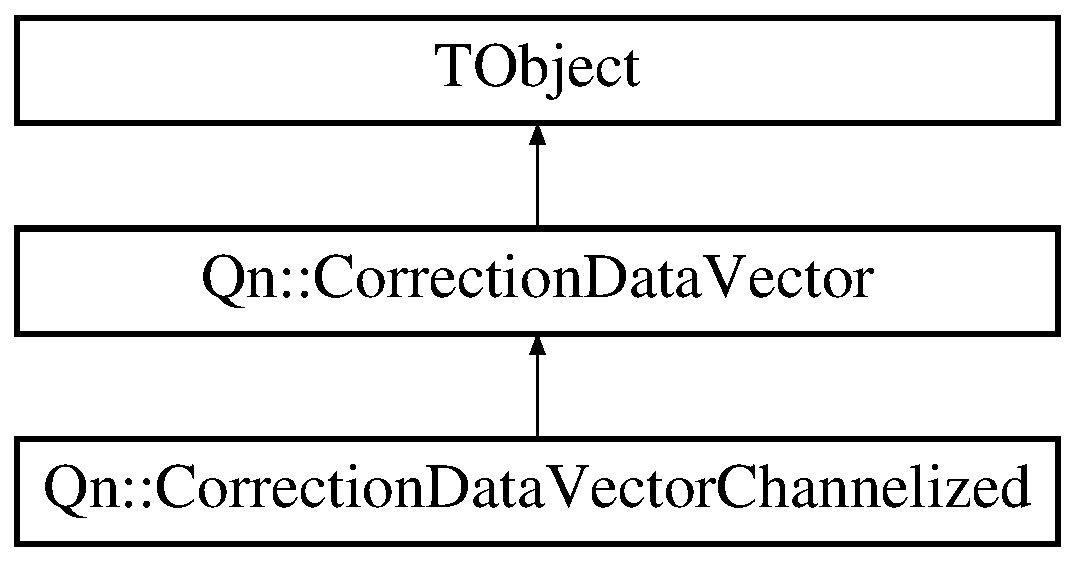
\includegraphics[height=3.000000cm]{classQn_1_1CorrectionDataVector}
\end{center}
\end{figure}
\subsection*{Public Member Functions}
\begin{DoxyCompactItemize}
\item 
\mbox{\Hypertarget{classQn_1_1CorrectionDataVector_a7fa749ad57305d5cf00076824a3a3fbc}\label{classQn_1_1CorrectionDataVector_a7fa749ad57305d5cf00076824a3a3fbc}} 
\mbox{\hyperlink{classQn_1_1CorrectionDataVector_a7fa749ad57305d5cf00076824a3a3fbc}{Correction\+Data\+Vector}} ()
\begin{DoxyCompactList}\small\item\em Default constructor. \end{DoxyCompactList}\item 
\mbox{\hyperlink{classQn_1_1CorrectionDataVector_afcdf4cec34dca08e9c567af6ecce00cf}{Correction\+Data\+Vector}} (Int\+\_\+t id, Float\+\_\+t phi, Float\+\_\+t weight)
\item 
\mbox{\Hypertarget{classQn_1_1CorrectionDataVector_ab78ea3730f98447536f86f4f7665efcd}\label{classQn_1_1CorrectionDataVector_ab78ea3730f98447536f86f4f7665efcd}} 
virtual \mbox{\hyperlink{classQn_1_1CorrectionDataVector_ab78ea3730f98447536f86f4f7665efcd}{$\sim$\+Correction\+Data\+Vector}} ()
\begin{DoxyCompactList}\small\item\em Default destructor. \end{DoxyCompactList}\item 
virtual void \mbox{\hyperlink{classQn_1_1CorrectionDataVector_aa2d415fd11a858c3c32c3fd820889bdc}{Set\+Phi}} (Float\+\_\+t phi)
\item 
void \mbox{\hyperlink{classQn_1_1CorrectionDataVector_a62c233a19220b9447412b6fb758a5732}{Set\+Id}} (Int\+\_\+t id)
\item 
Int\+\_\+t \mbox{\hyperlink{classQn_1_1CorrectionDataVector_a14c8e1a91eaeaff1fec89e80d715d07d}{Get\+Id}} ()
\item 
void \mbox{\hyperlink{classQn_1_1CorrectionDataVector_a4d71cb8911dd32d76ebc67250c24bac6}{Set\+Weight}} (Float\+\_\+t weight)
\item 
virtual Float\+\_\+t \mbox{\hyperlink{classQn_1_1CorrectionDataVector_a7b27c82f17e502100d8c83c642a161ec}{Phi}} ()
\item 
virtual Float\+\_\+t \mbox{\hyperlink{classQn_1_1CorrectionDataVector_a5fa5b765bd15afd5b5b7773ddb724e8e}{Weight}} ()
\item 
virtual Float\+\_\+t \mbox{\hyperlink{classQn_1_1CorrectionDataVector_a5c4b2b16cc814104974748db21a4cab5}{Equalized\+Weight}} ()
\end{DoxyCompactItemize}
\subsection*{Protected Attributes}
\begin{DoxyCompactItemize}
\item 
\mbox{\Hypertarget{classQn_1_1CorrectionDataVector_a6c21e4c45bfb08a6451e173b4df5f943}\label{classQn_1_1CorrectionDataVector_a6c21e4c45bfb08a6451e173b4df5f943}} 
Float\+\_\+t \mbox{\hyperlink{classQn_1_1CorrectionDataVector_a6c21e4c45bfb08a6451e173b4df5f943}{f\+Phi}}
\begin{DoxyCompactList}\small\item\em ! the azimuthal angle of the data vector \end{DoxyCompactList}\item 
\mbox{\Hypertarget{classQn_1_1CorrectionDataVector_ae06da92950b38fb4e08c3064865de842}\label{classQn_1_1CorrectionDataVector_ae06da92950b38fb4e08c3064865de842}} 
Int\+\_\+t \mbox{\hyperlink{classQn_1_1CorrectionDataVector_ae06da92950b38fb4e08c3064865de842}{f\+Id}}
\begin{DoxyCompactList}\small\item\em ! the id associated with the data vector \end{DoxyCompactList}\item 
\mbox{\Hypertarget{classQn_1_1CorrectionDataVector_a11619b9eb4043f1b90abdcfa080fd09f}\label{classQn_1_1CorrectionDataVector_a11619b9eb4043f1b90abdcfa080fd09f}} 
Float\+\_\+t \mbox{\hyperlink{classQn_1_1CorrectionDataVector_a11619b9eb4043f1b90abdcfa080fd09f}{f\+Weight}}
\begin{DoxyCompactList}\small\item\em ! raw weight assigned to the data vector \end{DoxyCompactList}\end{DoxyCompactItemize}
\subsection*{Static Protected Attributes}
\begin{DoxyCompactItemize}
\item 
\mbox{\Hypertarget{classQn_1_1CorrectionDataVector_a2a78df7f47caa805c4658f35157a2897}\label{classQn_1_1CorrectionDataVector_a2a78df7f47caa805c4658f35157a2897}} 
static const Float\+\_\+t \mbox{\hyperlink{classQn_1_1CorrectionDataVector_a2a78df7f47caa805c4658f35157a2897}{f\+Minimum\+Significant\+Value}} = 1.e-\/6
\begin{DoxyCompactList}\small\item\em the minimum value that will be considered as meaningful for processing \end{DoxyCompactList}\end{DoxyCompactItemize}


\subsection{Constructor \& Destructor Documentation}
\mbox{\Hypertarget{classQn_1_1CorrectionDataVector_afcdf4cec34dca08e9c567af6ecce00cf}\label{classQn_1_1CorrectionDataVector_afcdf4cec34dca08e9c567af6ecce00cf}} 
\index{Qn\+::\+Correction\+Data\+Vector@{Qn\+::\+Correction\+Data\+Vector}!Correction\+Data\+Vector@{Correction\+Data\+Vector}}
\index{Correction\+Data\+Vector@{Correction\+Data\+Vector}!Qn\+::\+Correction\+Data\+Vector@{Qn\+::\+Correction\+Data\+Vector}}
\subsubsection{\texorpdfstring{Correction\+Data\+Vector()}{CorrectionDataVector()}}
{\footnotesize\ttfamily Qn\+::\+Correction\+Data\+Vector\+::\+Correction\+Data\+Vector (\begin{DoxyParamCaption}\item[{Int\+\_\+t}]{id,  }\item[{Float\+\_\+t}]{phi,  }\item[{Float\+\_\+t}]{weight }\end{DoxyParamCaption})}

Normal constructor 
\begin{DoxyParams}{Parameters}
{\em id} & the id associated with the data vector \\
\hline
{\em phi} & the azimuthal angle \\
\hline
{\em weight} & the data vector weight \\
\hline
\end{DoxyParams}


\subsection{Member Function Documentation}
\mbox{\Hypertarget{classQn_1_1CorrectionDataVector_a5c4b2b16cc814104974748db21a4cab5}\label{classQn_1_1CorrectionDataVector_a5c4b2b16cc814104974748db21a4cab5}} 
\index{Qn\+::\+Correction\+Data\+Vector@{Qn\+::\+Correction\+Data\+Vector}!Equalized\+Weight@{Equalized\+Weight}}
\index{Equalized\+Weight@{Equalized\+Weight}!Qn\+::\+Correction\+Data\+Vector@{Qn\+::\+Correction\+Data\+Vector}}
\subsubsection{\texorpdfstring{Equalized\+Weight()}{EqualizedWeight()}}
{\footnotesize\ttfamily virtual Float\+\_\+t Qn\+::\+Correction\+Data\+Vector\+::\+Equalized\+Weight (\begin{DoxyParamCaption}{ }\end{DoxyParamCaption})\hspace{0.3cm}{\ttfamily [inline]}, {\ttfamily [virtual]}}

Gets the equalized weight for the data vector \begin{DoxyReturn}{Returns}
defaults to weights 
\end{DoxyReturn}


Reimplemented in \mbox{\hyperlink{classQn_1_1CorrectionDataVectorChannelized_a40656c301d6db91a2e761b129d746832}{Qn\+::\+Correction\+Data\+Vector\+Channelized}}.

\mbox{\Hypertarget{classQn_1_1CorrectionDataVector_a14c8e1a91eaeaff1fec89e80d715d07d}\label{classQn_1_1CorrectionDataVector_a14c8e1a91eaeaff1fec89e80d715d07d}} 
\index{Qn\+::\+Correction\+Data\+Vector@{Qn\+::\+Correction\+Data\+Vector}!Get\+Id@{Get\+Id}}
\index{Get\+Id@{Get\+Id}!Qn\+::\+Correction\+Data\+Vector@{Qn\+::\+Correction\+Data\+Vector}}
\subsubsection{\texorpdfstring{Get\+Id()}{GetId()}}
{\footnotesize\ttfamily Int\+\_\+t Qn\+::\+Correction\+Data\+Vector\+::\+Get\+Id (\begin{DoxyParamCaption}{ }\end{DoxyParamCaption})\hspace{0.3cm}{\ttfamily [inline]}}

Gets the channel id associated with the data vector \begin{DoxyReturn}{Returns}
the channel id 
\end{DoxyReturn}
\mbox{\Hypertarget{classQn_1_1CorrectionDataVector_a7b27c82f17e502100d8c83c642a161ec}\label{classQn_1_1CorrectionDataVector_a7b27c82f17e502100d8c83c642a161ec}} 
\index{Qn\+::\+Correction\+Data\+Vector@{Qn\+::\+Correction\+Data\+Vector}!Phi@{Phi}}
\index{Phi@{Phi}!Qn\+::\+Correction\+Data\+Vector@{Qn\+::\+Correction\+Data\+Vector}}
\subsubsection{\texorpdfstring{Phi()}{Phi()}}
{\footnotesize\ttfamily virtual Float\+\_\+t Qn\+::\+Correction\+Data\+Vector\+::\+Phi (\begin{DoxyParamCaption}{ }\end{DoxyParamCaption})\hspace{0.3cm}{\ttfamily [inline]}, {\ttfamily [virtual]}}

Gets the azimuthal angle for the data vector \begin{DoxyReturn}{Returns}
phi 
\end{DoxyReturn}
\mbox{\Hypertarget{classQn_1_1CorrectionDataVector_a62c233a19220b9447412b6fb758a5732}\label{classQn_1_1CorrectionDataVector_a62c233a19220b9447412b6fb758a5732}} 
\index{Qn\+::\+Correction\+Data\+Vector@{Qn\+::\+Correction\+Data\+Vector}!Set\+Id@{Set\+Id}}
\index{Set\+Id@{Set\+Id}!Qn\+::\+Correction\+Data\+Vector@{Qn\+::\+Correction\+Data\+Vector}}
\subsubsection{\texorpdfstring{Set\+Id()}{SetId()}}
{\footnotesize\ttfamily void Qn\+::\+Correction\+Data\+Vector\+::\+Set\+Id (\begin{DoxyParamCaption}\item[{Int\+\_\+t}]{id }\end{DoxyParamCaption})\hspace{0.3cm}{\ttfamily [inline]}}

Sets the channel id associated with the data vector 
\begin{DoxyParams}{Parameters}
{\em id} & channel id \\
\hline
\end{DoxyParams}
\mbox{\Hypertarget{classQn_1_1CorrectionDataVector_aa2d415fd11a858c3c32c3fd820889bdc}\label{classQn_1_1CorrectionDataVector_aa2d415fd11a858c3c32c3fd820889bdc}} 
\index{Qn\+::\+Correction\+Data\+Vector@{Qn\+::\+Correction\+Data\+Vector}!Set\+Phi@{Set\+Phi}}
\index{Set\+Phi@{Set\+Phi}!Qn\+::\+Correction\+Data\+Vector@{Qn\+::\+Correction\+Data\+Vector}}
\subsubsection{\texorpdfstring{Set\+Phi()}{SetPhi()}}
{\footnotesize\ttfamily virtual void Qn\+::\+Correction\+Data\+Vector\+::\+Set\+Phi (\begin{DoxyParamCaption}\item[{Float\+\_\+t}]{phi }\end{DoxyParamCaption})\hspace{0.3cm}{\ttfamily [inline]}, {\ttfamily [virtual]}}

Sets the data vector azimuthal angle 
\begin{DoxyParams}{Parameters}
{\em phi} & the azimuthal angle \\
\hline
\end{DoxyParams}
\mbox{\Hypertarget{classQn_1_1CorrectionDataVector_a4d71cb8911dd32d76ebc67250c24bac6}\label{classQn_1_1CorrectionDataVector_a4d71cb8911dd32d76ebc67250c24bac6}} 
\index{Qn\+::\+Correction\+Data\+Vector@{Qn\+::\+Correction\+Data\+Vector}!Set\+Weight@{Set\+Weight}}
\index{Set\+Weight@{Set\+Weight}!Qn\+::\+Correction\+Data\+Vector@{Qn\+::\+Correction\+Data\+Vector}}
\subsubsection{\texorpdfstring{Set\+Weight()}{SetWeight()}}
{\footnotesize\ttfamily void Qn\+::\+Correction\+Data\+Vector\+::\+Set\+Weight (\begin{DoxyParamCaption}\item[{Float\+\_\+t}]{weight }\end{DoxyParamCaption})\hspace{0.3cm}{\ttfamily [inline]}}

Sets the raw weight 
\begin{DoxyParams}{Parameters}
{\em weight} & raw weight from the detector channel \\
\hline
\end{DoxyParams}
\mbox{\Hypertarget{classQn_1_1CorrectionDataVector_a5fa5b765bd15afd5b5b7773ddb724e8e}\label{classQn_1_1CorrectionDataVector_a5fa5b765bd15afd5b5b7773ddb724e8e}} 
\index{Qn\+::\+Correction\+Data\+Vector@{Qn\+::\+Correction\+Data\+Vector}!Weight@{Weight}}
\index{Weight@{Weight}!Qn\+::\+Correction\+Data\+Vector@{Qn\+::\+Correction\+Data\+Vector}}
\subsubsection{\texorpdfstring{Weight()}{Weight()}}
{\footnotesize\ttfamily virtual Float\+\_\+t Qn\+::\+Correction\+Data\+Vector\+::\+Weight (\begin{DoxyParamCaption}{ }\end{DoxyParamCaption})\hspace{0.3cm}{\ttfamily [inline]}, {\ttfamily [virtual]}}

Gets the weight for the data vector \begin{DoxyReturn}{Returns}
defaults to 1.\+0 
\end{DoxyReturn}


Reimplemented in \mbox{\hyperlink{classQn_1_1CorrectionDataVectorChannelized_ad1ee46c787ccf5c6537f70f6458c3872}{Qn\+::\+Correction\+Data\+Vector\+Channelized}}.



The documentation for this class was generated from the following files\+:\begin{DoxyCompactItemize}
\item 
D\+T\+\_\+\+Flow/\+Qn\+Corrections/include/Correction\+Data\+Vector.\+h\item 
D\+T\+\_\+\+Flow/\+Qn\+Corrections/Correction\+Data\+Vector.\+cpp\end{DoxyCompactItemize}

\hypertarget{classQn_1_1CorrectionDataVectorChannelized}{}\section{Qn\+:\+:Correction\+Data\+Vector\+Channelized Class Reference}
\label{classQn_1_1CorrectionDataVectorChannelized}\index{Qn\+::\+Correction\+Data\+Vector\+Channelized@{Qn\+::\+Correction\+Data\+Vector\+Channelized}}
Inheritance diagram for Qn\+:\+:Correction\+Data\+Vector\+Channelized\+:\begin{figure}[H]
\begin{center}
\leavevmode
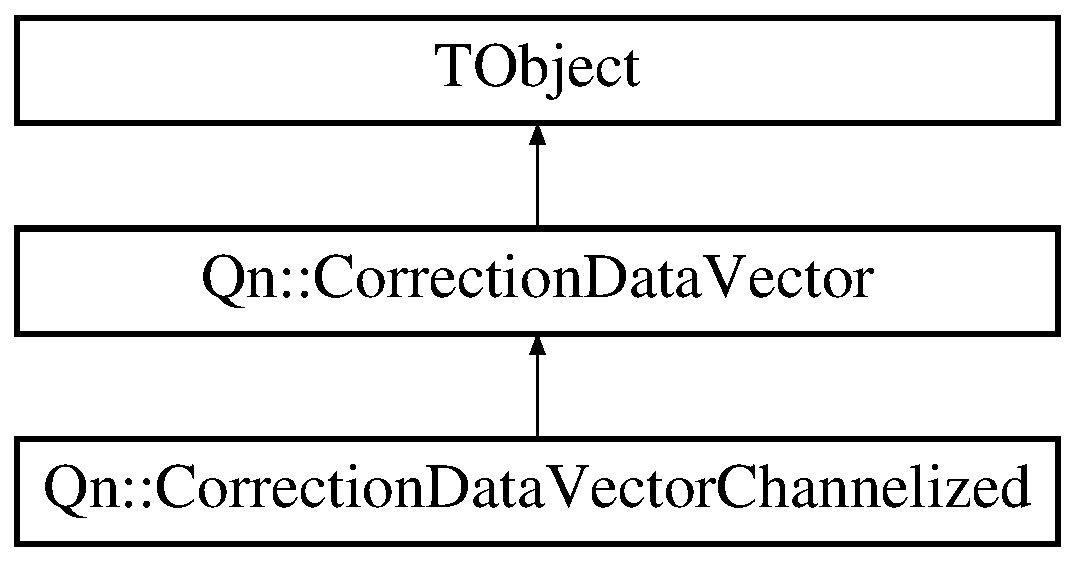
\includegraphics[height=3.000000cm]{classQn_1_1CorrectionDataVectorChannelized}
\end{center}
\end{figure}
\subsection*{Public Member Functions}
\begin{DoxyCompactItemize}
\item 
\mbox{\Hypertarget{classQn_1_1CorrectionDataVectorChannelized_ad020992f1c0d70f6eaaabd4d6997a25b}\label{classQn_1_1CorrectionDataVectorChannelized_ad020992f1c0d70f6eaaabd4d6997a25b}} 
\mbox{\hyperlink{classQn_1_1CorrectionDataVectorChannelized_ad020992f1c0d70f6eaaabd4d6997a25b}{Correction\+Data\+Vector\+Channelized}} ()
\begin{DoxyCompactList}\small\item\em Default constructor. \end{DoxyCompactList}\item 
\mbox{\hyperlink{classQn_1_1CorrectionDataVectorChannelized_a5e3f5b06e8199d86b9ceab8e97c5e3a3}{Correction\+Data\+Vector\+Channelized}} (Int\+\_\+t channel\+Id, Float\+\_\+t phi, Float\+\_\+t weight)
\item 
\mbox{\Hypertarget{classQn_1_1CorrectionDataVectorChannelized_a9ca1281cbf59c1bd96b6605bfa0925d4}\label{classQn_1_1CorrectionDataVectorChannelized_a9ca1281cbf59c1bd96b6605bfa0925d4}} 
virtual \mbox{\hyperlink{classQn_1_1CorrectionDataVectorChannelized_a9ca1281cbf59c1bd96b6605bfa0925d4}{$\sim$\+Correction\+Data\+Vector\+Channelized}} ()
\begin{DoxyCompactList}\small\item\em Default destructor. \end{DoxyCompactList}\item 
void \mbox{\hyperlink{classQn_1_1CorrectionDataVectorChannelized_af7f71996404eb417e7e3e006938b0fd9}{Set\+Equalized\+Weight}} (Float\+\_\+t weight)
\item 
virtual Float\+\_\+t \mbox{\hyperlink{classQn_1_1CorrectionDataVectorChannelized_ad1ee46c787ccf5c6537f70f6458c3872}{Weight}} ()
\item 
virtual Float\+\_\+t \mbox{\hyperlink{classQn_1_1CorrectionDataVectorChannelized_a40656c301d6db91a2e761b129d746832}{Equalized\+Weight}} ()
\end{DoxyCompactItemize}
\subsection*{Additional Inherited Members}


\subsection{Constructor \& Destructor Documentation}
\mbox{\Hypertarget{classQn_1_1CorrectionDataVectorChannelized_a5e3f5b06e8199d86b9ceab8e97c5e3a3}\label{classQn_1_1CorrectionDataVectorChannelized_a5e3f5b06e8199d86b9ceab8e97c5e3a3}} 
\index{Qn\+::\+Correction\+Data\+Vector\+Channelized@{Qn\+::\+Correction\+Data\+Vector\+Channelized}!Correction\+Data\+Vector\+Channelized@{Correction\+Data\+Vector\+Channelized}}
\index{Correction\+Data\+Vector\+Channelized@{Correction\+Data\+Vector\+Channelized}!Qn\+::\+Correction\+Data\+Vector\+Channelized@{Qn\+::\+Correction\+Data\+Vector\+Channelized}}
\subsubsection{\texorpdfstring{Correction\+Data\+Vector\+Channelized()}{CorrectionDataVectorChannelized()}}
{\footnotesize\ttfamily Qn\+::\+Correction\+Data\+Vector\+Channelized\+::\+Correction\+Data\+Vector\+Channelized (\begin{DoxyParamCaption}\item[{Int\+\_\+t}]{channel\+Id,  }\item[{Float\+\_\+t}]{phi,  }\item[{Float\+\_\+t}]{weight }\end{DoxyParamCaption})}

Normal constructor 
\begin{DoxyParams}{Parameters}
{\em channel\+Id} & channel number \\
\hline
{\em phi} & the azimuthal angle \\
\hline
{\em weight} & the data vector weight \\
\hline
\end{DoxyParams}


\subsection{Member Function Documentation}
\mbox{\Hypertarget{classQn_1_1CorrectionDataVectorChannelized_a40656c301d6db91a2e761b129d746832}\label{classQn_1_1CorrectionDataVectorChannelized_a40656c301d6db91a2e761b129d746832}} 
\index{Qn\+::\+Correction\+Data\+Vector\+Channelized@{Qn\+::\+Correction\+Data\+Vector\+Channelized}!Equalized\+Weight@{Equalized\+Weight}}
\index{Equalized\+Weight@{Equalized\+Weight}!Qn\+::\+Correction\+Data\+Vector\+Channelized@{Qn\+::\+Correction\+Data\+Vector\+Channelized}}
\subsubsection{\texorpdfstring{Equalized\+Weight()}{EqualizedWeight()}}
{\footnotesize\ttfamily virtual Float\+\_\+t Qn\+::\+Correction\+Data\+Vector\+Channelized\+::\+Equalized\+Weight (\begin{DoxyParamCaption}{ }\end{DoxyParamCaption})\hspace{0.3cm}{\ttfamily [inline]}, {\ttfamily [virtual]}}

Gets the equalized weight for the data vector \begin{DoxyReturn}{Returns}
the equalized weight 
\end{DoxyReturn}


Reimplemented from \mbox{\hyperlink{classQn_1_1CorrectionDataVector_a5c4b2b16cc814104974748db21a4cab5}{Qn\+::\+Correction\+Data\+Vector}}.

\mbox{\Hypertarget{classQn_1_1CorrectionDataVectorChannelized_af7f71996404eb417e7e3e006938b0fd9}\label{classQn_1_1CorrectionDataVectorChannelized_af7f71996404eb417e7e3e006938b0fd9}} 
\index{Qn\+::\+Correction\+Data\+Vector\+Channelized@{Qn\+::\+Correction\+Data\+Vector\+Channelized}!Set\+Equalized\+Weight@{Set\+Equalized\+Weight}}
\index{Set\+Equalized\+Weight@{Set\+Equalized\+Weight}!Qn\+::\+Correction\+Data\+Vector\+Channelized@{Qn\+::\+Correction\+Data\+Vector\+Channelized}}
\subsubsection{\texorpdfstring{Set\+Equalized\+Weight()}{SetEqualizedWeight()}}
{\footnotesize\ttfamily void Qn\+::\+Correction\+Data\+Vector\+Channelized\+::\+Set\+Equalized\+Weight (\begin{DoxyParamCaption}\item[{Float\+\_\+t}]{weight }\end{DoxyParamCaption})\hspace{0.3cm}{\ttfamily [inline]}}

Sets the equalized weight 
\begin{DoxyParams}{Parameters}
{\em weight} & equalized weight after channel equalization \\
\hline
\end{DoxyParams}
\mbox{\Hypertarget{classQn_1_1CorrectionDataVectorChannelized_ad1ee46c787ccf5c6537f70f6458c3872}\label{classQn_1_1CorrectionDataVectorChannelized_ad1ee46c787ccf5c6537f70f6458c3872}} 
\index{Qn\+::\+Correction\+Data\+Vector\+Channelized@{Qn\+::\+Correction\+Data\+Vector\+Channelized}!Weight@{Weight}}
\index{Weight@{Weight}!Qn\+::\+Correction\+Data\+Vector\+Channelized@{Qn\+::\+Correction\+Data\+Vector\+Channelized}}
\subsubsection{\texorpdfstring{Weight()}{Weight()}}
{\footnotesize\ttfamily virtual Float\+\_\+t Qn\+::\+Correction\+Data\+Vector\+Channelized\+::\+Weight (\begin{DoxyParamCaption}{ }\end{DoxyParamCaption})\hspace{0.3cm}{\ttfamily [inline]}, {\ttfamily [virtual]}}

Gets the weight for the data vector \begin{DoxyReturn}{Returns}
the raw weight 
\end{DoxyReturn}


Reimplemented from \mbox{\hyperlink{classQn_1_1CorrectionDataVector_a5fa5b765bd15afd5b5b7773ddb724e8e}{Qn\+::\+Correction\+Data\+Vector}}.



The documentation for this class was generated from the following files\+:\begin{DoxyCompactItemize}
\item 
D\+T\+\_\+\+Flow/\+Qn\+Corrections/include/Correction\+Data\+Vector\+Channelized.\+h\item 
D\+T\+\_\+\+Flow/\+Qn\+Corrections/Correction\+Data\+Vector\+Channelized.\+cpp\end{DoxyCompactItemize}

\hypertarget{classQn_1_1CorrectionDetector}{}\section{Qn\+:\+:Correction\+Detector Class Reference}
\label{classQn_1_1CorrectionDetector}\index{Qn\+::\+Correction\+Detector@{Qn\+::\+Correction\+Detector}}
Inheritance diagram for Qn\+:\+:Correction\+Detector\+:\begin{figure}[H]
\begin{center}
\leavevmode
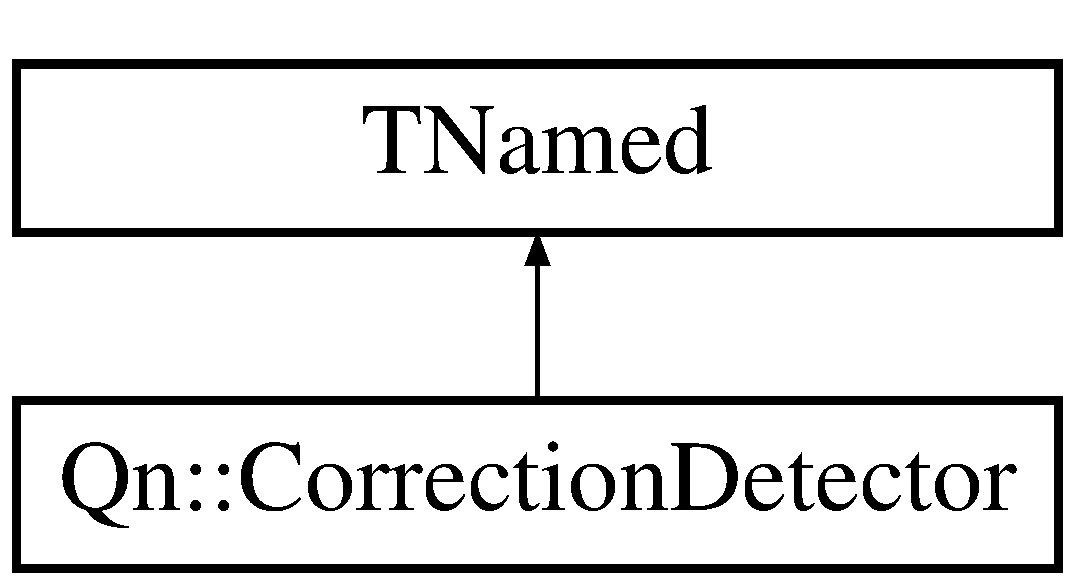
\includegraphics[height=2.000000cm]{classQn_1_1CorrectionDetector}
\end{center}
\end{figure}
\subsection*{Public Member Functions}
\begin{DoxyCompactItemize}
\item 
\mbox{\Hypertarget{classQn_1_1CorrectionDetector_a58413afb9c1be0e4ddf602aa351fe00f}\label{classQn_1_1CorrectionDetector_a58413afb9c1be0e4ddf602aa351fe00f}} 
\mbox{\hyperlink{classQn_1_1CorrectionDetector_a58413afb9c1be0e4ddf602aa351fe00f}{Correction\+Detector}} ()
\begin{DoxyCompactList}\small\item\em Default constructor. \end{DoxyCompactList}\item 
\mbox{\hyperlink{classQn_1_1CorrectionDetector_a50aa008a5c92d7773d8b9851806ddb19}{Correction\+Detector}} (const char $\ast$name, Int\+\_\+t id)
\item 
virtual \mbox{\hyperlink{classQn_1_1CorrectionDetector_a90e172fc836adae967b808cb75be3ca3}{$\sim$\+Correction\+Detector}} ()
\item 
Int\+\_\+t \mbox{\hyperlink{classQn_1_1CorrectionDetector_a8f3d562c17ea64048e7830683387588c}{Get\+Id}} ()
\item 
void \mbox{\hyperlink{classQn_1_1CorrectionDetector_a7858076955dbbffabbe3092f9936f51a}{Create\+Support\+Data\+Structures}} ()
\item 
Bool\+\_\+t \mbox{\hyperlink{classQn_1_1CorrectionDetector_a401cd8059027ee1f06eb96de414edc0c}{Create\+Support\+Histograms}} (T\+List $\ast$list)
\item 
Bool\+\_\+t \mbox{\hyperlink{classQn_1_1CorrectionDetector_a3670d14b0e6fc446631c87dc5bb0d12b}{Create\+Q\+A\+Histograms}} (T\+List $\ast$list)
\item 
Bool\+\_\+t \mbox{\hyperlink{classQn_1_1CorrectionDetector_a24c31acbd10eaf982a10b304390de47c}{Create\+Nve\+Q\+A\+Histograms}} (T\+List $\ast$list)
\item 
Bool\+\_\+t \mbox{\hyperlink{classQn_1_1CorrectionDetector_a9348902c90054c1f1d262081c2818b2e}{Attach\+Correction\+Inputs}} (T\+List $\ast$list)
\item 
virtual void \mbox{\hyperlink{classQn_1_1CorrectionDetector_a9cd7dd2c1a6d5d8cb7a1a0a18f3f5ee3}{After\+Inputs\+Attach\+Actions}} ()
\item 
Bool\+\_\+t \mbox{\hyperlink{classQn_1_1CorrectionDetector_a4942a3b1f05f8a7f4d899e6ae9808338}{Process\+Corrections}} (const double $\ast$variable\+Container)
\item 
Bool\+\_\+t \mbox{\hyperlink{classQn_1_1CorrectionDetector_a8415d9c428d7a168cc953da44b6a5e01}{Process\+Data\+Collection}} (const double $\ast$variable\+Container)
\item 
void \mbox{\hyperlink{classQn_1_1CorrectionDetector_a46b40b3743208bcf3cddd063690985e8}{Include\+Qn\+Vectors}} (T\+List $\ast$list)
\item 
const char $\ast$ \mbox{\hyperlink{classQn_1_1CorrectionDetector_a02acf1eeed47ab5eb2df84ae1de57b59}{Get\+Accepted\+Data\+Detector\+Configuration\+Name}} (Int\+\_\+t index) const
\item 
void \mbox{\hyperlink{classQn_1_1CorrectionDetector_a8de962ff8acbffdcfb15eba90a3a91ed}{Attach\+Corrections\+Manager}} (\mbox{\hyperlink{classQn_1_1CorrectionCalculator}{Correction\+Calculator}} $\ast$manager)
\item 
void \mbox{\hyperlink{classQn_1_1CorrectionDetector_a029dd33340f261a48a2c7fb32c599e7f}{Add\+Detector\+Configuration}} (\mbox{\hyperlink{classQn_1_1DetectorConfiguration}{Detector\+Configuration}} $\ast$detector\+Configuration)
\item 
\mbox{\hyperlink{classQn_1_1DetectorConfiguration}{Detector\+Configuration}} $\ast$ \mbox{\hyperlink{classQn_1_1CorrectionDetector_a5b4d3b18be6dd94a86e56d838c42ca80}{Find\+Detector\+Configuration}} (const char $\ast$name)
\item 
void \mbox{\hyperlink{classQn_1_1CorrectionDetector_a7605d01ec9abe6675b325d6ae2d710e9}{Fill\+Detector\+Configuration\+Name\+List}} (T\+List $\ast$list) const
\item 
void \mbox{\hyperlink{classQn_1_1CorrectionDetector_af4426ef9b524025c09e6f78a156b8f5d}{Fill\+Overall\+Input\+Correction\+Step\+List}} (T\+List $\ast$list) const
\item 
void \mbox{\hyperlink{classQn_1_1CorrectionDetector_a5a6b9787279e397b1682e72038acd3fe}{Fill\+Overall\+Qn\+Vector\+Correction\+Step\+List}} (T\+List $\ast$list) const
\item 
virtual void \mbox{\hyperlink{classQn_1_1CorrectionDetector_afbfcc072f1ba0d4b6c42a62daeb5a58e}{Report\+On\+Corrections}} (T\+List $\ast$steps, T\+List $\ast$calib, T\+List $\ast$apply) const
\item 
Int\+\_\+t \mbox{\hyperlink{classQn_1_1CorrectionDetector_a94328e4e2b21ac573c9f32d2d9a3e24a}{Add\+Data\+Vector}} (const double $\ast$variable\+Container, Double\+\_\+t phi, Double\+\_\+t weight=1.\+0, Int\+\_\+t channel\+Id=-\/1)
\item 
virtual void \mbox{\hyperlink{classQn_1_1CorrectionDetector_a9ff746e0a0128405bb37ffc0384fe114}{Clear\+Detector}} ()
\end{DoxyCompactItemize}


\subsection{Constructor \& Destructor Documentation}
\mbox{\Hypertarget{classQn_1_1CorrectionDetector_a50aa008a5c92d7773d8b9851806ddb19}\label{classQn_1_1CorrectionDetector_a50aa008a5c92d7773d8b9851806ddb19}} 
\index{Qn\+::\+Correction\+Detector@{Qn\+::\+Correction\+Detector}!Correction\+Detector@{Correction\+Detector}}
\index{Correction\+Detector@{Correction\+Detector}!Qn\+::\+Correction\+Detector@{Qn\+::\+Correction\+Detector}}
\subsubsection{\texorpdfstring{Correction\+Detector()}{CorrectionDetector()}}
{\footnotesize\ttfamily Qn\+::\+Correction\+Detector\+::\+Correction\+Detector (\begin{DoxyParamCaption}\item[{const char $\ast$}]{name,  }\item[{Int\+\_\+t}]{id }\end{DoxyParamCaption})}

Normal constructor 
\begin{DoxyParams}{Parameters}
{\em name} & the name of the detector \\
\hline
{\em id} & detector Id \\
\hline
\end{DoxyParams}
\mbox{\Hypertarget{classQn_1_1CorrectionDetector_a90e172fc836adae967b808cb75be3ca3}\label{classQn_1_1CorrectionDetector_a90e172fc836adae967b808cb75be3ca3}} 
\index{Qn\+::\+Correction\+Detector@{Qn\+::\+Correction\+Detector}!````~Correction\+Detector@{$\sim$\+Correction\+Detector}}
\index{````~Correction\+Detector@{$\sim$\+Correction\+Detector}!Qn\+::\+Correction\+Detector@{Qn\+::\+Correction\+Detector}}
\subsubsection{\texorpdfstring{$\sim$\+Correction\+Detector()}{~CorrectionDetector()}}
{\footnotesize\ttfamily Qn\+::\+Correction\+Detector\+::$\sim$\+Correction\+Detector (\begin{DoxyParamCaption}{ }\end{DoxyParamCaption})\hspace{0.3cm}{\ttfamily [virtual]}}

Default destructor The detector class does not own anything 

\subsection{Member Function Documentation}
\mbox{\Hypertarget{classQn_1_1CorrectionDetector_a94328e4e2b21ac573c9f32d2d9a3e24a}\label{classQn_1_1CorrectionDetector_a94328e4e2b21ac573c9f32d2d9a3e24a}} 
\index{Qn\+::\+Correction\+Detector@{Qn\+::\+Correction\+Detector}!Add\+Data\+Vector@{Add\+Data\+Vector}}
\index{Add\+Data\+Vector@{Add\+Data\+Vector}!Qn\+::\+Correction\+Detector@{Qn\+::\+Correction\+Detector}}
\subsubsection{\texorpdfstring{Add\+Data\+Vector()}{AddDataVector()}}
{\footnotesize\ttfamily Int\+\_\+t Qn\+::\+Correction\+Detector\+::\+Add\+Data\+Vector (\begin{DoxyParamCaption}\item[{const double $\ast$}]{variable\+Container,  }\item[{Double\+\_\+t}]{phi,  }\item[{Double\+\_\+t}]{weight = {\ttfamily 1.0},  }\item[{Int\+\_\+t}]{channel\+Id = {\ttfamily -\/1} }\end{DoxyParamCaption})\hspace{0.3cm}{\ttfamily [inline]}}

New data vector for the detector The request is transmitted to the attached detector configurations. The current content of the variable bank is passed in order to check for optional cuts tha define the detector configurations. 
\begin{DoxyParams}{Parameters}
{\em variable\+Container} & pointer to the variable content bank \\
\hline
{\em phi} & azimuthal angle \\
\hline
{\em weight} & the weight of the data vector \\
\hline
{\em channel\+Id} & the channel Id that originates the data vector \\
\hline
\end{DoxyParams}
\begin{DoxyReturn}{Returns}
the number of detector configurations that accepted and stored the data vector 
\end{DoxyReturn}
\mbox{\Hypertarget{classQn_1_1CorrectionDetector_a029dd33340f261a48a2c7fb32c599e7f}\label{classQn_1_1CorrectionDetector_a029dd33340f261a48a2c7fb32c599e7f}} 
\index{Qn\+::\+Correction\+Detector@{Qn\+::\+Correction\+Detector}!Add\+Detector\+Configuration@{Add\+Detector\+Configuration}}
\index{Add\+Detector\+Configuration@{Add\+Detector\+Configuration}!Qn\+::\+Correction\+Detector@{Qn\+::\+Correction\+Detector}}
\subsubsection{\texorpdfstring{Add\+Detector\+Configuration()}{AddDetectorConfiguration()}}
{\footnotesize\ttfamily void Qn\+::\+Correction\+Detector\+::\+Add\+Detector\+Configuration (\begin{DoxyParamCaption}\item[{\mbox{\hyperlink{classQn_1_1DetectorConfiguration}{Detector\+Configuration}} $\ast$}]{detector\+Configuration }\end{DoxyParamCaption})}

Adds a new detector configuration to the current detector

Raise an execution error if the configuration detector reference is not empty and if the detector configuration is already incorporated to the detector. 
\begin{DoxyParams}{Parameters}
{\em detector\+Configuration} & pointer to the configuration to be added \\
\hline
\end{DoxyParams}
\mbox{\Hypertarget{classQn_1_1CorrectionDetector_a9cd7dd2c1a6d5d8cb7a1a0a18f3f5ee3}\label{classQn_1_1CorrectionDetector_a9cd7dd2c1a6d5d8cb7a1a0a18f3f5ee3}} 
\index{Qn\+::\+Correction\+Detector@{Qn\+::\+Correction\+Detector}!After\+Inputs\+Attach\+Actions@{After\+Inputs\+Attach\+Actions}}
\index{After\+Inputs\+Attach\+Actions@{After\+Inputs\+Attach\+Actions}!Qn\+::\+Correction\+Detector@{Qn\+::\+Correction\+Detector}}
\subsubsection{\texorpdfstring{After\+Inputs\+Attach\+Actions()}{AfterInputsAttachActions()}}
{\footnotesize\ttfamily void Qn\+::\+Correction\+Detector\+::\+After\+Inputs\+Attach\+Actions (\begin{DoxyParamCaption}{ }\end{DoxyParamCaption})\hspace{0.3cm}{\ttfamily [virtual]}}

Perform after calibration histograms attach actions It is used to inform the different correction step that all conditions for running the network are in place so it is time to check if their requirements are satisfied

The request is transmitted to the attached detector configurations \mbox{\Hypertarget{classQn_1_1CorrectionDetector_a9348902c90054c1f1d262081c2818b2e}\label{classQn_1_1CorrectionDetector_a9348902c90054c1f1d262081c2818b2e}} 
\index{Qn\+::\+Correction\+Detector@{Qn\+::\+Correction\+Detector}!Attach\+Correction\+Inputs@{Attach\+Correction\+Inputs}}
\index{Attach\+Correction\+Inputs@{Attach\+Correction\+Inputs}!Qn\+::\+Correction\+Detector@{Qn\+::\+Correction\+Detector}}
\subsubsection{\texorpdfstring{Attach\+Correction\+Inputs()}{AttachCorrectionInputs()}}
{\footnotesize\ttfamily Bool\+\_\+t Qn\+::\+Correction\+Detector\+::\+Attach\+Correction\+Inputs (\begin{DoxyParamCaption}\item[{T\+List $\ast$}]{list }\end{DoxyParamCaption})}

Asks for attaching the needed input information to the correction steps

The request is transmitted to the attached detector configurations 
\begin{DoxyParams}{Parameters}
{\em list} & list where the input information should be found \\
\hline
\end{DoxyParams}
\begin{DoxyReturn}{Returns}
k\+T\+R\+UE if everything went OK 
\end{DoxyReturn}
\mbox{\Hypertarget{classQn_1_1CorrectionDetector_a8de962ff8acbffdcfb15eba90a3a91ed}\label{classQn_1_1CorrectionDetector_a8de962ff8acbffdcfb15eba90a3a91ed}} 
\index{Qn\+::\+Correction\+Detector@{Qn\+::\+Correction\+Detector}!Attach\+Corrections\+Manager@{Attach\+Corrections\+Manager}}
\index{Attach\+Corrections\+Manager@{Attach\+Corrections\+Manager}!Qn\+::\+Correction\+Detector@{Qn\+::\+Correction\+Detector}}
\subsubsection{\texorpdfstring{Attach\+Corrections\+Manager()}{AttachCorrectionsManager()}}
{\footnotesize\ttfamily void Qn\+::\+Correction\+Detector\+::\+Attach\+Corrections\+Manager (\begin{DoxyParamCaption}\item[{\mbox{\hyperlink{classQn_1_1CorrectionCalculator}{Correction\+Calculator}} $\ast$}]{manager }\end{DoxyParamCaption})}

Stores the framework manager pointer and transmits it to the incorporated detector configurations if any


\begin{DoxyParams}{Parameters}
{\em manager} & the framework manager \\
\hline
\end{DoxyParams}
\mbox{\Hypertarget{classQn_1_1CorrectionDetector_a9ff746e0a0128405bb37ffc0384fe114}\label{classQn_1_1CorrectionDetector_a9ff746e0a0128405bb37ffc0384fe114}} 
\index{Qn\+::\+Correction\+Detector@{Qn\+::\+Correction\+Detector}!Clear\+Detector@{Clear\+Detector}}
\index{Clear\+Detector@{Clear\+Detector}!Qn\+::\+Correction\+Detector@{Qn\+::\+Correction\+Detector}}
\subsubsection{\texorpdfstring{Clear\+Detector()}{ClearDetector()}}
{\footnotesize\ttfamily void Qn\+::\+Correction\+Detector\+::\+Clear\+Detector (\begin{DoxyParamCaption}{ }\end{DoxyParamCaption})\hspace{0.3cm}{\ttfamily [inline]}, {\ttfamily [virtual]}}

Clean the detector to accept a new event

Transfers the order to the detector configurations \mbox{\Hypertarget{classQn_1_1CorrectionDetector_a24c31acbd10eaf982a10b304390de47c}\label{classQn_1_1CorrectionDetector_a24c31acbd10eaf982a10b304390de47c}} 
\index{Qn\+::\+Correction\+Detector@{Qn\+::\+Correction\+Detector}!Create\+Nve\+Q\+A\+Histograms@{Create\+Nve\+Q\+A\+Histograms}}
\index{Create\+Nve\+Q\+A\+Histograms@{Create\+Nve\+Q\+A\+Histograms}!Qn\+::\+Correction\+Detector@{Qn\+::\+Correction\+Detector}}
\subsubsection{\texorpdfstring{Create\+Nve\+Q\+A\+Histograms()}{CreateNveQAHistograms()}}
{\footnotesize\ttfamily Bool\+\_\+t Qn\+::\+Correction\+Detector\+::\+Create\+Nve\+Q\+A\+Histograms (\begin{DoxyParamCaption}\item[{T\+List $\ast$}]{list }\end{DoxyParamCaption})}

Asks for non validated entries QA histograms creation

The request is transmitted to the attached detector configurations 
\begin{DoxyParams}{Parameters}
{\em list} & list where the histograms should be incorporated for its persistence \\
\hline
\end{DoxyParams}
\begin{DoxyReturn}{Returns}
k\+T\+R\+UE if everything went OK 
\end{DoxyReturn}
\mbox{\Hypertarget{classQn_1_1CorrectionDetector_a3670d14b0e6fc446631c87dc5bb0d12b}\label{classQn_1_1CorrectionDetector_a3670d14b0e6fc446631c87dc5bb0d12b}} 
\index{Qn\+::\+Correction\+Detector@{Qn\+::\+Correction\+Detector}!Create\+Q\+A\+Histograms@{Create\+Q\+A\+Histograms}}
\index{Create\+Q\+A\+Histograms@{Create\+Q\+A\+Histograms}!Qn\+::\+Correction\+Detector@{Qn\+::\+Correction\+Detector}}
\subsubsection{\texorpdfstring{Create\+Q\+A\+Histograms()}{CreateQAHistograms()}}
{\footnotesize\ttfamily Bool\+\_\+t Qn\+::\+Correction\+Detector\+::\+Create\+Q\+A\+Histograms (\begin{DoxyParamCaption}\item[{T\+List $\ast$}]{list }\end{DoxyParamCaption})}

Asks for QA histograms creation

The request is transmitted to the attached detector configurations 
\begin{DoxyParams}{Parameters}
{\em list} & list where the histograms should be incorporated for its persistence \\
\hline
\end{DoxyParams}
\begin{DoxyReturn}{Returns}
k\+T\+R\+UE if everything went OK 
\end{DoxyReturn}
\mbox{\Hypertarget{classQn_1_1CorrectionDetector_a7858076955dbbffabbe3092f9936f51a}\label{classQn_1_1CorrectionDetector_a7858076955dbbffabbe3092f9936f51a}} 
\index{Qn\+::\+Correction\+Detector@{Qn\+::\+Correction\+Detector}!Create\+Support\+Data\+Structures@{Create\+Support\+Data\+Structures}}
\index{Create\+Support\+Data\+Structures@{Create\+Support\+Data\+Structures}!Qn\+::\+Correction\+Detector@{Qn\+::\+Correction\+Detector}}
\subsubsection{\texorpdfstring{Create\+Support\+Data\+Structures()}{CreateSupportDataStructures()}}
{\footnotesize\ttfamily void Qn\+::\+Correction\+Detector\+::\+Create\+Support\+Data\+Structures (\begin{DoxyParamCaption}{ }\end{DoxyParamCaption})}

Asks for support data structures creation

The request is transmitted to the attached detector configurations \mbox{\Hypertarget{classQn_1_1CorrectionDetector_a401cd8059027ee1f06eb96de414edc0c}\label{classQn_1_1CorrectionDetector_a401cd8059027ee1f06eb96de414edc0c}} 
\index{Qn\+::\+Correction\+Detector@{Qn\+::\+Correction\+Detector}!Create\+Support\+Histograms@{Create\+Support\+Histograms}}
\index{Create\+Support\+Histograms@{Create\+Support\+Histograms}!Qn\+::\+Correction\+Detector@{Qn\+::\+Correction\+Detector}}
\subsubsection{\texorpdfstring{Create\+Support\+Histograms()}{CreateSupportHistograms()}}
{\footnotesize\ttfamily Bool\+\_\+t Qn\+::\+Correction\+Detector\+::\+Create\+Support\+Histograms (\begin{DoxyParamCaption}\item[{T\+List $\ast$}]{list }\end{DoxyParamCaption})}

Asks for support histograms creation

The request is transmitted to the attached detector configurations 
\begin{DoxyParams}{Parameters}
{\em list} & list where the histograms should be incorporated for its persistence \\
\hline
\end{DoxyParams}
\begin{DoxyReturn}{Returns}
k\+T\+R\+UE if everything went OK 
\end{DoxyReturn}
\mbox{\Hypertarget{classQn_1_1CorrectionDetector_a7605d01ec9abe6675b325d6ae2d710e9}\label{classQn_1_1CorrectionDetector_a7605d01ec9abe6675b325d6ae2d710e9}} 
\index{Qn\+::\+Correction\+Detector@{Qn\+::\+Correction\+Detector}!Fill\+Detector\+Configuration\+Name\+List@{Fill\+Detector\+Configuration\+Name\+List}}
\index{Fill\+Detector\+Configuration\+Name\+List@{Fill\+Detector\+Configuration\+Name\+List}!Qn\+::\+Correction\+Detector@{Qn\+::\+Correction\+Detector}}
\subsubsection{\texorpdfstring{Fill\+Detector\+Configuration\+Name\+List()}{FillDetectorConfigurationNameList()}}
{\footnotesize\ttfamily void Qn\+::\+Correction\+Detector\+::\+Fill\+Detector\+Configuration\+Name\+List (\begin{DoxyParamCaption}\item[{T\+List $\ast$}]{list }\end{DoxyParamCaption}) const}

Include the name of each detector configuration into the passed list


\begin{DoxyParams}{Parameters}
{\em list} & the list where to incorporate detector configurations name \\
\hline
\end{DoxyParams}
\mbox{\Hypertarget{classQn_1_1CorrectionDetector_af4426ef9b524025c09e6f78a156b8f5d}\label{classQn_1_1CorrectionDetector_af4426ef9b524025c09e6f78a156b8f5d}} 
\index{Qn\+::\+Correction\+Detector@{Qn\+::\+Correction\+Detector}!Fill\+Overall\+Input\+Correction\+Step\+List@{Fill\+Overall\+Input\+Correction\+Step\+List}}
\index{Fill\+Overall\+Input\+Correction\+Step\+List@{Fill\+Overall\+Input\+Correction\+Step\+List}!Qn\+::\+Correction\+Detector@{Qn\+::\+Correction\+Detector}}
\subsubsection{\texorpdfstring{Fill\+Overall\+Input\+Correction\+Step\+List()}{FillOverallInputCorrectionStepList()}}
{\footnotesize\ttfamily void Qn\+::\+Correction\+Detector\+::\+Fill\+Overall\+Input\+Correction\+Step\+List (\begin{DoxyParamCaption}\item[{T\+List $\ast$}]{list }\end{DoxyParamCaption}) const}

Include the name of the input correction steps on each detector configuration into the passed list

The request is transmitted to the attached detector configurations 
\begin{DoxyParams}{Parameters}
{\em list} & list where the corrected \mbox{\hyperlink{namespaceQn}{Qn}} vector should be added \\
\hline
\end{DoxyParams}
\mbox{\Hypertarget{classQn_1_1CorrectionDetector_a5a6b9787279e397b1682e72038acd3fe}\label{classQn_1_1CorrectionDetector_a5a6b9787279e397b1682e72038acd3fe}} 
\index{Qn\+::\+Correction\+Detector@{Qn\+::\+Correction\+Detector}!Fill\+Overall\+Qn\+Vector\+Correction\+Step\+List@{Fill\+Overall\+Qn\+Vector\+Correction\+Step\+List}}
\index{Fill\+Overall\+Qn\+Vector\+Correction\+Step\+List@{Fill\+Overall\+Qn\+Vector\+Correction\+Step\+List}!Qn\+::\+Correction\+Detector@{Qn\+::\+Correction\+Detector}}
\subsubsection{\texorpdfstring{Fill\+Overall\+Qn\+Vector\+Correction\+Step\+List()}{FillOverallQnVectorCorrectionStepList()}}
{\footnotesize\ttfamily void Qn\+::\+Correction\+Detector\+::\+Fill\+Overall\+Qn\+Vector\+Correction\+Step\+List (\begin{DoxyParamCaption}\item[{T\+List $\ast$}]{list }\end{DoxyParamCaption}) const}

Include the name of the \mbox{\hyperlink{namespaceQn}{Qn}} vector correction steps on each detector configuration into the passed list

The request is transmitted to the attached detector configurations 
\begin{DoxyParams}{Parameters}
{\em list} & list where the corrected \mbox{\hyperlink{namespaceQn}{Qn}} vector should be added \\
\hline
\end{DoxyParams}
\mbox{\Hypertarget{classQn_1_1CorrectionDetector_a5b4d3b18be6dd94a86e56d838c42ca80}\label{classQn_1_1CorrectionDetector_a5b4d3b18be6dd94a86e56d838c42ca80}} 
\index{Qn\+::\+Correction\+Detector@{Qn\+::\+Correction\+Detector}!Find\+Detector\+Configuration@{Find\+Detector\+Configuration}}
\index{Find\+Detector\+Configuration@{Find\+Detector\+Configuration}!Qn\+::\+Correction\+Detector@{Qn\+::\+Correction\+Detector}}
\subsubsection{\texorpdfstring{Find\+Detector\+Configuration()}{FindDetectorConfiguration()}}
{\footnotesize\ttfamily \mbox{\hyperlink{classQn_1_1DetectorConfiguration}{Detector\+Configuration}} $\ast$ Qn\+::\+Correction\+Detector\+::\+Find\+Detector\+Configuration (\begin{DoxyParamCaption}\item[{const char $\ast$}]{name }\end{DoxyParamCaption})}

Searches for a concrete detector configuration by name 
\begin{DoxyParams}{Parameters}
{\em name} & the name of the detector configuration to find \\
\hline
\end{DoxyParams}
\begin{DoxyReturn}{Returns}
pointer to the found detector configuration (N\+U\+LL if not found) 
\end{DoxyReturn}
\mbox{\Hypertarget{classQn_1_1CorrectionDetector_a02acf1eeed47ab5eb2df84ae1de57b59}\label{classQn_1_1CorrectionDetector_a02acf1eeed47ab5eb2df84ae1de57b59}} 
\index{Qn\+::\+Correction\+Detector@{Qn\+::\+Correction\+Detector}!Get\+Accepted\+Data\+Detector\+Configuration\+Name@{Get\+Accepted\+Data\+Detector\+Configuration\+Name}}
\index{Get\+Accepted\+Data\+Detector\+Configuration\+Name@{Get\+Accepted\+Data\+Detector\+Configuration\+Name}!Qn\+::\+Correction\+Detector@{Qn\+::\+Correction\+Detector}}
\subsubsection{\texorpdfstring{Get\+Accepted\+Data\+Detector\+Configuration\+Name()}{GetAcceptedDataDetectorConfigurationName()}}
{\footnotesize\ttfamily const char$\ast$ Qn\+::\+Correction\+Detector\+::\+Get\+Accepted\+Data\+Detector\+Configuration\+Name (\begin{DoxyParamCaption}\item[{Int\+\_\+t}]{index }\end{DoxyParamCaption}) const\hspace{0.3cm}{\ttfamily [inline]}}

Gets the name of the detector configuration at index that accepted last data vector 
\begin{DoxyParams}{Parameters}
{\em index} & the position in the list of accepted data vector configuration \\
\hline
\end{DoxyParams}
\begin{DoxyReturn}{Returns}
the configuration name 
\end{DoxyReturn}
\mbox{\Hypertarget{classQn_1_1CorrectionDetector_a8f3d562c17ea64048e7830683387588c}\label{classQn_1_1CorrectionDetector_a8f3d562c17ea64048e7830683387588c}} 
\index{Qn\+::\+Correction\+Detector@{Qn\+::\+Correction\+Detector}!Get\+Id@{Get\+Id}}
\index{Get\+Id@{Get\+Id}!Qn\+::\+Correction\+Detector@{Qn\+::\+Correction\+Detector}}
\subsubsection{\texorpdfstring{Get\+Id()}{GetId()}}
{\footnotesize\ttfamily Int\+\_\+t Qn\+::\+Correction\+Detector\+::\+Get\+Id (\begin{DoxyParamCaption}{ }\end{DoxyParamCaption})\hspace{0.3cm}{\ttfamily [inline]}}

Gets the detector Id

\begin{DoxyReturn}{Returns}
detector Id 
\end{DoxyReturn}
\mbox{\Hypertarget{classQn_1_1CorrectionDetector_a46b40b3743208bcf3cddd063690985e8}\label{classQn_1_1CorrectionDetector_a46b40b3743208bcf3cddd063690985e8}} 
\index{Qn\+::\+Correction\+Detector@{Qn\+::\+Correction\+Detector}!Include\+Qn\+Vectors@{Include\+Qn\+Vectors}}
\index{Include\+Qn\+Vectors@{Include\+Qn\+Vectors}!Qn\+::\+Correction\+Detector@{Qn\+::\+Correction\+Detector}}
\subsubsection{\texorpdfstring{Include\+Qn\+Vectors()}{IncludeQnVectors()}}
{\footnotesize\ttfamily void Qn\+::\+Correction\+Detector\+::\+Include\+Qn\+Vectors (\begin{DoxyParamCaption}\item[{T\+List $\ast$}]{list }\end{DoxyParamCaption})}

Include the the list of \mbox{\hyperlink{namespaceQn}{Qn}} vector associated to the detector into the passed list

The request is transmitted to the attached detector configurations 
\begin{DoxyParams}{Parameters}
{\em list} & list where the corrected \mbox{\hyperlink{namespaceQn}{Qn}} vector should be added \\
\hline
\end{DoxyParams}
\mbox{\Hypertarget{classQn_1_1CorrectionDetector_a4942a3b1f05f8a7f4d899e6ae9808338}\label{classQn_1_1CorrectionDetector_a4942a3b1f05f8a7f4d899e6ae9808338}} 
\index{Qn\+::\+Correction\+Detector@{Qn\+::\+Correction\+Detector}!Process\+Corrections@{Process\+Corrections}}
\index{Process\+Corrections@{Process\+Corrections}!Qn\+::\+Correction\+Detector@{Qn\+::\+Correction\+Detector}}
\subsubsection{\texorpdfstring{Process\+Corrections()}{ProcessCorrections()}}
{\footnotesize\ttfamily Bool\+\_\+t Qn\+::\+Correction\+Detector\+::\+Process\+Corrections (\begin{DoxyParamCaption}\item[{const double $\ast$}]{variable\+Container }\end{DoxyParamCaption})\hspace{0.3cm}{\ttfamily [inline]}}

Ask for processing corrections for the involved detector

The request is transmitted to the attached detector configurations \begin{DoxyReturn}{Returns}
k\+T\+R\+UE if everything went OK 
\end{DoxyReturn}
\mbox{\Hypertarget{classQn_1_1CorrectionDetector_a8415d9c428d7a168cc953da44b6a5e01}\label{classQn_1_1CorrectionDetector_a8415d9c428d7a168cc953da44b6a5e01}} 
\index{Qn\+::\+Correction\+Detector@{Qn\+::\+Correction\+Detector}!Process\+Data\+Collection@{Process\+Data\+Collection}}
\index{Process\+Data\+Collection@{Process\+Data\+Collection}!Qn\+::\+Correction\+Detector@{Qn\+::\+Correction\+Detector}}
\subsubsection{\texorpdfstring{Process\+Data\+Collection()}{ProcessDataCollection()}}
{\footnotesize\ttfamily Bool\+\_\+t Qn\+::\+Correction\+Detector\+::\+Process\+Data\+Collection (\begin{DoxyParamCaption}\item[{const double $\ast$}]{variable\+Container }\end{DoxyParamCaption})\hspace{0.3cm}{\ttfamily [inline]}}

Ask for processing corrections data collection for the involved detector

The request is transmitted to the attached detector configurations \begin{DoxyReturn}{Returns}
k\+T\+R\+UE if everything went OK 
\end{DoxyReturn}
\mbox{\Hypertarget{classQn_1_1CorrectionDetector_afbfcc072f1ba0d4b6c42a62daeb5a58e}\label{classQn_1_1CorrectionDetector_afbfcc072f1ba0d4b6c42a62daeb5a58e}} 
\index{Qn\+::\+Correction\+Detector@{Qn\+::\+Correction\+Detector}!Report\+On\+Corrections@{Report\+On\+Corrections}}
\index{Report\+On\+Corrections@{Report\+On\+Corrections}!Qn\+::\+Correction\+Detector@{Qn\+::\+Correction\+Detector}}
\subsubsection{\texorpdfstring{Report\+On\+Corrections()}{ReportOnCorrections()}}
{\footnotesize\ttfamily void Qn\+::\+Correction\+Detector\+::\+Report\+On\+Corrections (\begin{DoxyParamCaption}\item[{T\+List $\ast$}]{steps,  }\item[{T\+List $\ast$}]{calib,  }\item[{T\+List $\ast$}]{apply }\end{DoxyParamCaption}) const\hspace{0.3cm}{\ttfamily [virtual]}}

Provide information about assigned corrections on each of the detector configurations

The request is transmitted to the attached detector configurations 
\begin{DoxyParams}{Parameters}
{\em steps} & list for incorporating the list of assigned correction steps \\
\hline
{\em calib} & list for incorporating the list of steps in calibrating status \\
\hline
{\em apply} & list for incorporating the list of steps in applying status \\
\hline
\end{DoxyParams}


The documentation for this class was generated from the following files\+:\begin{DoxyCompactItemize}
\item 
D\+T\+\_\+\+Flow/\+Qn\+Corrections/include/Correction\+Detector.\+h\item 
D\+T\+\_\+\+Flow/\+Qn\+Corrections/Correction\+Detector.\+cpp\end{DoxyCompactItemize}

\hypertarget{classQn_1_1CorrectionHistogram}{}\section{Qn\+:\+:Correction\+Histogram Class Reference}
\label{classQn_1_1CorrectionHistogram}\index{Qn\+::\+Correction\+Histogram@{Qn\+::\+Correction\+Histogram}}
Inheritance diagram for Qn\+:\+:Correction\+Histogram\+:\begin{figure}[H]
\begin{center}
\leavevmode
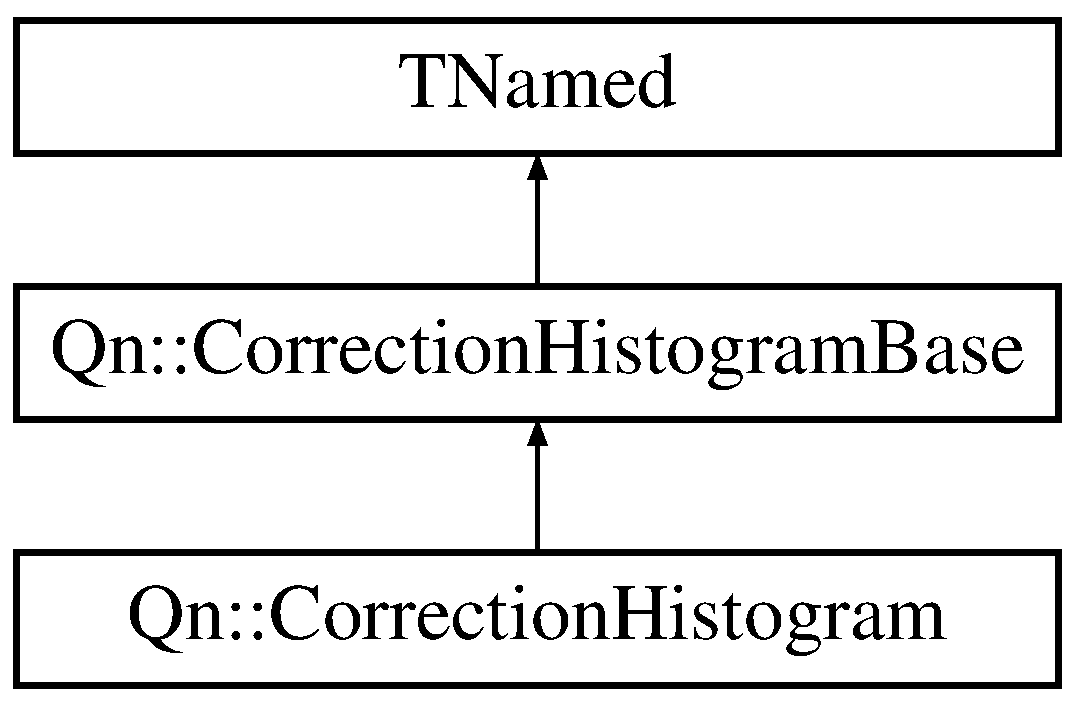
\includegraphics[height=3.000000cm]{classQn_1_1CorrectionHistogram}
\end{center}
\end{figure}
\subsection*{Public Member Functions}
\begin{DoxyCompactItemize}
\item 
\mbox{\Hypertarget{classQn_1_1CorrectionHistogram_afb136f75daee32c8969c1c53a4fb4802}\label{classQn_1_1CorrectionHistogram_afb136f75daee32c8969c1c53a4fb4802}} 
\mbox{\hyperlink{classQn_1_1CorrectionHistogram_afb136f75daee32c8969c1c53a4fb4802}{Correction\+Histogram}} ()
\begin{DoxyCompactList}\small\item\em Default constructor. \end{DoxyCompactList}\item 
\mbox{\hyperlink{classQn_1_1CorrectionHistogram_acefd77dc11928421955bd2c8550ff817}{Correction\+Histogram}} (const char $\ast$name, const char $\ast$title, \mbox{\hyperlink{classQn_1_1EventClassVariablesSet}{Event\+Class\+Variables\+Set}} \&ecvs)
\item 
virtual \mbox{\hyperlink{classQn_1_1CorrectionHistogram_a328b703cceadfac67d51947ce27992da}{$\sim$\+Correction\+Histogram}} ()
\item 
Bool\+\_\+t \mbox{\hyperlink{classQn_1_1CorrectionHistogram_a5d7baa24476a584ad144923ec2bec7a5}{Create\+Histogram}} (T\+List $\ast$histogram\+List)
\item 
virtual Long64\+\_\+t \mbox{\hyperlink{classQn_1_1CorrectionHistogram_ac67e334f0d4bae4c45727e129c9bfba1}{Get\+Bin}} (const double $\ast$variable\+Container)
\item 
\mbox{\Hypertarget{classQn_1_1CorrectionHistogram_a008557e4ab70595b83f60973acc37be2}\label{classQn_1_1CorrectionHistogram_a008557e4ab70595b83f60973acc37be2}} 
virtual Long64\+\_\+t \mbox{\hyperlink{classQn_1_1CorrectionHistogram_a008557e4ab70595b83f60973acc37be2}{Get\+Bin}} (const double $\ast$variable\+Container, Int\+\_\+t n\+Channel)
\begin{DoxyCompactList}\small\item\em wrong call for this class invoke base class behaviour \end{DoxyCompactList}\item 
virtual Bool\+\_\+t \mbox{\hyperlink{classQn_1_1CorrectionHistogram_a26d4a5cb3aebf1c447bba10359224a62}{Bin\+Content\+Validated}} (Long64\+\_\+t bin)
\item 
virtual Float\+\_\+t \mbox{\hyperlink{classQn_1_1CorrectionHistogram_a469c7ca13b740d1224dcaf5c9a41eb2b}{Get\+Bin\+Content}} (Long64\+\_\+t bin)
\item 
virtual Float\+\_\+t \mbox{\hyperlink{classQn_1_1CorrectionHistogram_ac9feeeb4721f0b199c5c96e41224836e}{Get\+Bin\+Error}} (Long64\+\_\+t bin)
\item 
virtual void \mbox{\hyperlink{classQn_1_1CorrectionHistogram_a3704882797e987dc62c31d953f49ec7e}{Fill}} (const double $\ast$variable\+Container, Float\+\_\+t weight)
\item 
\mbox{\Hypertarget{classQn_1_1CorrectionHistogram_a5686f074e8b72ce0faae1c266d1eee9f}\label{classQn_1_1CorrectionHistogram_a5686f074e8b72ce0faae1c266d1eee9f}} 
virtual void \mbox{\hyperlink{classQn_1_1CorrectionHistogram_a5686f074e8b72ce0faae1c266d1eee9f}{Fill}} (const double $\ast$variable\+Container, Int\+\_\+t n\+Channel, Float\+\_\+t weight)
\begin{DoxyCompactList}\small\item\em wrong call for this class invoke base class behavior \end{DoxyCompactList}\end{DoxyCompactItemize}
\subsection*{Additional Inherited Members}


\subsection{Constructor \& Destructor Documentation}
\mbox{\Hypertarget{classQn_1_1CorrectionHistogram_acefd77dc11928421955bd2c8550ff817}\label{classQn_1_1CorrectionHistogram_acefd77dc11928421955bd2c8550ff817}} 
\index{Qn\+::\+Correction\+Histogram@{Qn\+::\+Correction\+Histogram}!Correction\+Histogram@{Correction\+Histogram}}
\index{Correction\+Histogram@{Correction\+Histogram}!Qn\+::\+Correction\+Histogram@{Qn\+::\+Correction\+Histogram}}
\subsubsection{\texorpdfstring{Correction\+Histogram()}{CorrectionHistogram()}}
{\footnotesize\ttfamily Qn\+::\+Correction\+Histogram\+::\+Correction\+Histogram (\begin{DoxyParamCaption}\item[{const char $\ast$}]{name,  }\item[{const char $\ast$}]{title,  }\item[{\mbox{\hyperlink{classQn_1_1EventClassVariablesSet}{Event\+Class\+Variables\+Set}} \&}]{ecvs }\end{DoxyParamCaption})}

Normal constructor

Stores the set of variables that identify the different event classes passing them to its parent and prepares the object for actual histogram creation or attachment


\begin{DoxyParams}{Parameters}
{\em name} & base for the name of the histograms \\
\hline
{\em title} & base for the title of the histograms \\
\hline
{\em ecvs} & the event classes variables set \\
\hline
\end{DoxyParams}
\mbox{\Hypertarget{classQn_1_1CorrectionHistogram_a328b703cceadfac67d51947ce27992da}\label{classQn_1_1CorrectionHistogram_a328b703cceadfac67d51947ce27992da}} 
\index{Qn\+::\+Correction\+Histogram@{Qn\+::\+Correction\+Histogram}!````~Correction\+Histogram@{$\sim$\+Correction\+Histogram}}
\index{````~Correction\+Histogram@{$\sim$\+Correction\+Histogram}!Qn\+::\+Correction\+Histogram@{Qn\+::\+Correction\+Histogram}}
\subsubsection{\texorpdfstring{$\sim$\+Correction\+Histogram()}{~CorrectionHistogram()}}
{\footnotesize\ttfamily Qn\+::\+Correction\+Histogram\+::$\sim$\+Correction\+Histogram (\begin{DoxyParamCaption}{ }\end{DoxyParamCaption})\hspace{0.3cm}{\ttfamily [virtual]}}

Default destructor Releases the memory taken 

\subsection{Member Function Documentation}
\mbox{\Hypertarget{classQn_1_1CorrectionHistogram_a26d4a5cb3aebf1c447bba10359224a62}\label{classQn_1_1CorrectionHistogram_a26d4a5cb3aebf1c447bba10359224a62}} 
\index{Qn\+::\+Correction\+Histogram@{Qn\+::\+Correction\+Histogram}!Bin\+Content\+Validated@{Bin\+Content\+Validated}}
\index{Bin\+Content\+Validated@{Bin\+Content\+Validated}!Qn\+::\+Correction\+Histogram@{Qn\+::\+Correction\+Histogram}}
\subsubsection{\texorpdfstring{Bin\+Content\+Validated()}{BinContentValidated()}}
{\footnotesize\ttfamily Bool\+\_\+t Qn\+::\+Correction\+Histogram\+::\+Bin\+Content\+Validated (\begin{DoxyParamCaption}\item[{Long64\+\_\+t}]{bin }\end{DoxyParamCaption})\hspace{0.3cm}{\ttfamily [virtual]}}

Check the validity of the content of the passed bin This kind of histograms cannot validate the bin content so, it is always valid. 
\begin{DoxyParams}{Parameters}
{\em bin} & the bin to check its content validity \\
\hline
\end{DoxyParams}
\begin{DoxyReturn}{Returns}
k\+T\+R\+UE if the content is valid k\+F\+A\+L\+SE otherwise 
\end{DoxyReturn}


Implements \mbox{\hyperlink{classQn_1_1CorrectionHistogramBase_a4db2c92ceaffefaa91475a721612d80d}{Qn\+::\+Correction\+Histogram\+Base}}.

\mbox{\Hypertarget{classQn_1_1CorrectionHistogram_a5d7baa24476a584ad144923ec2bec7a5}\label{classQn_1_1CorrectionHistogram_a5d7baa24476a584ad144923ec2bec7a5}} 
\index{Qn\+::\+Correction\+Histogram@{Qn\+::\+Correction\+Histogram}!Create\+Histogram@{Create\+Histogram}}
\index{Create\+Histogram@{Create\+Histogram}!Qn\+::\+Correction\+Histogram@{Qn\+::\+Correction\+Histogram}}
\subsubsection{\texorpdfstring{Create\+Histogram()}{CreateHistogram()}}
{\footnotesize\ttfamily Bool\+\_\+t Qn\+::\+Correction\+Histogram\+::\+Create\+Histogram (\begin{DoxyParamCaption}\item[{T\+List $\ast$}]{histogram\+List }\end{DoxyParamCaption})}

Creates the support histogram for the histogram function

Based in the event classes variables set in the parent class the values multidimensional histogram is created.

The histogram is added to the passed histogram list


\begin{DoxyParams}{Parameters}
{\em histogram\+List} & list where the histograms have to be added \\
\hline
\end{DoxyParams}
\begin{DoxyReturn}{Returns}
true if properly created 
\end{DoxyReturn}
\mbox{\Hypertarget{classQn_1_1CorrectionHistogram_a3704882797e987dc62c31d953f49ec7e}\label{classQn_1_1CorrectionHistogram_a3704882797e987dc62c31d953f49ec7e}} 
\index{Qn\+::\+Correction\+Histogram@{Qn\+::\+Correction\+Histogram}!Fill@{Fill}}
\index{Fill@{Fill}!Qn\+::\+Correction\+Histogram@{Qn\+::\+Correction\+Histogram}}
\subsubsection{\texorpdfstring{Fill()}{Fill()}}
{\footnotesize\ttfamily void Qn\+::\+Correction\+Histogram\+::\+Fill (\begin{DoxyParamCaption}\item[{const double $\ast$}]{variable\+Container,  }\item[{Float\+\_\+t}]{weight }\end{DoxyParamCaption})\hspace{0.3cm}{\ttfamily [virtual]}}

Fills the histogram

The involved bin is computed according to the current variables content and the passed external channel number. The bin is then increased by the given weight.


\begin{DoxyParams}{Parameters}
{\em variable\+Container} & the current variables content addressed by var Id \\
\hline
{\em weight} & the increment in the bin content \\
\hline
\end{DoxyParams}


Reimplemented from \mbox{\hyperlink{classQn_1_1CorrectionHistogramBase_a16b7518942714780ec9ceb56bb517f0f}{Qn\+::\+Correction\+Histogram\+Base}}.

\mbox{\Hypertarget{classQn_1_1CorrectionHistogram_ac67e334f0d4bae4c45727e129c9bfba1}\label{classQn_1_1CorrectionHistogram_ac67e334f0d4bae4c45727e129c9bfba1}} 
\index{Qn\+::\+Correction\+Histogram@{Qn\+::\+Correction\+Histogram}!Get\+Bin@{Get\+Bin}}
\index{Get\+Bin@{Get\+Bin}!Qn\+::\+Correction\+Histogram@{Qn\+::\+Correction\+Histogram}}
\subsubsection{\texorpdfstring{Get\+Bin()}{GetBin()}}
{\footnotesize\ttfamily Long64\+\_\+t Qn\+::\+Correction\+Histogram\+::\+Get\+Bin (\begin{DoxyParamCaption}\item[{const double $\ast$}]{variable\+Container }\end{DoxyParamCaption})\hspace{0.3cm}{\ttfamily [virtual]}}

Get the bin number for the current variable content

The bin number identifies the event class the current variable content points to under the passed channel.


\begin{DoxyParams}{Parameters}
{\em variable\+Container} & the current variables content addressed by var Id \\
\hline
\end{DoxyParams}
\begin{DoxyReturn}{Returns}
the associated bin to the current variables content 
\end{DoxyReturn}


Reimplemented from \mbox{\hyperlink{classQn_1_1CorrectionHistogramBase_ab1f64550f4e1812864da6f9f6ea565e6}{Qn\+::\+Correction\+Histogram\+Base}}.

\mbox{\Hypertarget{classQn_1_1CorrectionHistogram_a469c7ca13b740d1224dcaf5c9a41eb2b}\label{classQn_1_1CorrectionHistogram_a469c7ca13b740d1224dcaf5c9a41eb2b}} 
\index{Qn\+::\+Correction\+Histogram@{Qn\+::\+Correction\+Histogram}!Get\+Bin\+Content@{Get\+Bin\+Content}}
\index{Get\+Bin\+Content@{Get\+Bin\+Content}!Qn\+::\+Correction\+Histogram@{Qn\+::\+Correction\+Histogram}}
\subsubsection{\texorpdfstring{Get\+Bin\+Content()}{GetBinContent()}}
{\footnotesize\ttfamily Float\+\_\+t Qn\+::\+Correction\+Histogram\+::\+Get\+Bin\+Content (\begin{DoxyParamCaption}\item[{Long64\+\_\+t}]{bin }\end{DoxyParamCaption})\hspace{0.3cm}{\ttfamily [virtual]}}

Get the bin content for the passed bin number

The bin number identifies a desired event class whose content is requested.


\begin{DoxyParams}{Parameters}
{\em bin} & the interested bin number \\
\hline
\end{DoxyParams}
\begin{DoxyReturn}{Returns}
the bin number content 
\end{DoxyReturn}


Reimplemented from \mbox{\hyperlink{classQn_1_1CorrectionHistogramBase_a9e4e745a6f4cbebf5b9277d6d63bc9c7}{Qn\+::\+Correction\+Histogram\+Base}}.

\mbox{\Hypertarget{classQn_1_1CorrectionHistogram_ac9feeeb4721f0b199c5c96e41224836e}\label{classQn_1_1CorrectionHistogram_ac9feeeb4721f0b199c5c96e41224836e}} 
\index{Qn\+::\+Correction\+Histogram@{Qn\+::\+Correction\+Histogram}!Get\+Bin\+Error@{Get\+Bin\+Error}}
\index{Get\+Bin\+Error@{Get\+Bin\+Error}!Qn\+::\+Correction\+Histogram@{Qn\+::\+Correction\+Histogram}}
\subsubsection{\texorpdfstring{Get\+Bin\+Error()}{GetBinError()}}
{\footnotesize\ttfamily Float\+\_\+t Qn\+::\+Correction\+Histogram\+::\+Get\+Bin\+Error (\begin{DoxyParamCaption}\item[{Long64\+\_\+t}]{bin }\end{DoxyParamCaption})\hspace{0.3cm}{\ttfamily [virtual]}}

Get the bin content error for the passed bin number

The bin number identifies a desired event class whose content error is requested.


\begin{DoxyParams}{Parameters}
{\em bin} & the interested bin number \\
\hline
\end{DoxyParams}
\begin{DoxyReturn}{Returns}
the bin number content error 
\end{DoxyReturn}


Reimplemented from \mbox{\hyperlink{classQn_1_1CorrectionHistogramBase_a50a7dd4c5bbe5e4d0e405365c2a9104d}{Qn\+::\+Correction\+Histogram\+Base}}.



The documentation for this class was generated from the following files\+:\begin{DoxyCompactItemize}
\item 
D\+T\+\_\+\+Flow/\+Qn\+Corrections/include/Correction\+Histogram.\+h\item 
D\+T\+\_\+\+Flow/\+Qn\+Corrections/Correction\+Histogram.\+cpp\end{DoxyCompactItemize}

\hypertarget{classQn_1_1CorrectionHistogramBase}{}\section{Qn\+:\+:Correction\+Histogram\+Base Class Reference}
\label{classQn_1_1CorrectionHistogramBase}\index{Qn\+::\+Correction\+Histogram\+Base@{Qn\+::\+Correction\+Histogram\+Base}}
Inheritance diagram for Qn\+:\+:Correction\+Histogram\+Base\+:\begin{figure}[H]
\begin{center}
\leavevmode
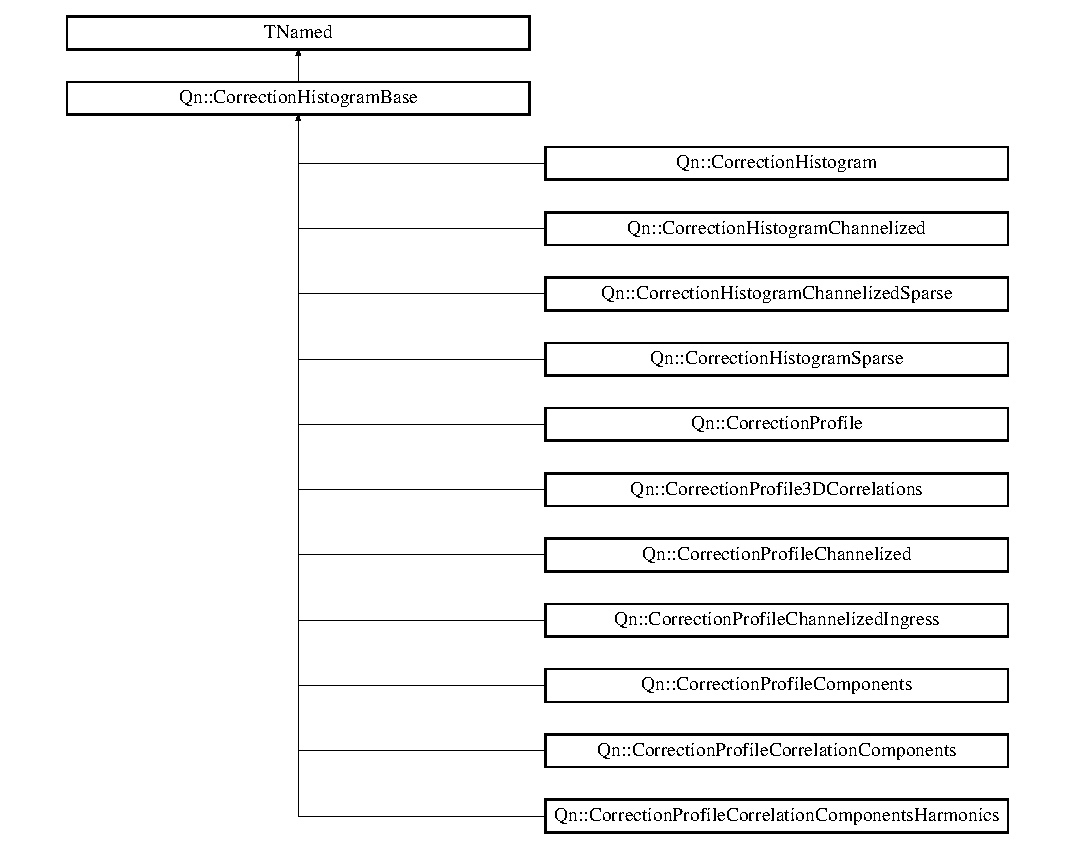
\includegraphics[height=10.963856cm]{classQn_1_1CorrectionHistogramBase}
\end{center}
\end{figure}
\subsection*{Public Member Functions}
\begin{DoxyCompactItemize}
\item 
\mbox{\Hypertarget{classQn_1_1CorrectionHistogramBase_a55ffedbb27258f2bf1e662f828f9501c}\label{classQn_1_1CorrectionHistogramBase_a55ffedbb27258f2bf1e662f828f9501c}} 
\mbox{\hyperlink{classQn_1_1CorrectionHistogramBase_a55ffedbb27258f2bf1e662f828f9501c}{Correction\+Histogram\+Base}} ()
\begin{DoxyCompactList}\small\item\em Default constructor. \end{DoxyCompactList}\item 
\mbox{\hyperlink{classQn_1_1CorrectionHistogramBase_ae60d38510dda50104d646b2c28da24f8}{Correction\+Histogram\+Base}} (const char $\ast$name, const char $\ast$title, \mbox{\hyperlink{classQn_1_1EventClassVariablesSet}{Event\+Class\+Variables\+Set}} \&ecvs, Option\+\_\+t $\ast$option=\char`\"{}\char`\"{})
\item 
virtual \mbox{\hyperlink{classQn_1_1CorrectionHistogramBase_ad938c894b552cda9e368c756b9462f70}{$\sim$\+Correction\+Histogram\+Base}} ()
\item 
virtual Bool\+\_\+t \mbox{\hyperlink{classQn_1_1CorrectionHistogramBase_ad8bcd0079fe5db561780a522e46b7b16}{Attach\+Histograms}} (T\+List $\ast$histogram\+List)
\item 
virtual Bool\+\_\+t \mbox{\hyperlink{classQn_1_1CorrectionHistogramBase_afa979697b43e2ebd0580a3359b2aca63}{Attach\+Histograms}} (T\+List $\ast$histogram\+List, const Bool\+\_\+t $\ast$b\+Used\+Channel, const Int\+\_\+t $\ast$n\+Channel\+Group)
\item 
virtual Long64\+\_\+t \mbox{\hyperlink{classQn_1_1CorrectionHistogramBase_ab1f64550f4e1812864da6f9f6ea565e6}{Get\+Bin}} (const double $\ast$variable\+Container)
\item 
virtual Long64\+\_\+t \mbox{\hyperlink{classQn_1_1CorrectionHistogramBase_acfde166908e4da950470841f21f87fb9}{Get\+Bin}} (const double $\ast$variable\+Container, Int\+\_\+t n\+Channel)
\item 
virtual Bool\+\_\+t \mbox{\hyperlink{classQn_1_1CorrectionHistogramBase_a4db2c92ceaffefaa91475a721612d80d}{Bin\+Content\+Validated}} (Long64\+\_\+t bin)=0
\item 
virtual void \mbox{\hyperlink{classQn_1_1CorrectionHistogramBase_ab398bab718b21e952de6dd84fbaef683}{Set\+No\+Of\+Entries\+Threshold}} (Int\+\_\+t n\+No\+Of\+Entries)
\item 
virtual Float\+\_\+t \mbox{\hyperlink{classQn_1_1CorrectionHistogramBase_a9e4e745a6f4cbebf5b9277d6d63bc9c7}{Get\+Bin\+Content}} (Long64\+\_\+t bin)
\item 
virtual Float\+\_\+t \mbox{\hyperlink{classQn_1_1CorrectionHistogramBase_a3dc485a3ac0767a04691a228b3189b95}{Get\+X\+Bin\+Content}} (Int\+\_\+t harmonic, Long64\+\_\+t bin)
\item 
virtual Float\+\_\+t \mbox{\hyperlink{classQn_1_1CorrectionHistogramBase_acc898b8b375f88d0625798d3b9a9b9ba}{Get\+Y\+Bin\+Content}} (Int\+\_\+t harmonic, Long64\+\_\+t bin)
\item 
virtual Float\+\_\+t \mbox{\hyperlink{classQn_1_1CorrectionHistogramBase_a5ed53d98b57fa9e9ec4de78ae518d9d9}{Get\+X\+X\+Bin\+Content}} (Long64\+\_\+t bin)
\item 
virtual Float\+\_\+t \mbox{\hyperlink{classQn_1_1CorrectionHistogramBase_aa631b6234a81dbe46b29a95fda339b69}{Get\+X\+Y\+Bin\+Content}} (Long64\+\_\+t bin)
\item 
virtual Float\+\_\+t \mbox{\hyperlink{classQn_1_1CorrectionHistogramBase_a2bc9c26889a5ff0479f5638e2e253174}{Get\+Y\+X\+Bin\+Content}} (Long64\+\_\+t bin)
\item 
virtual Float\+\_\+t \mbox{\hyperlink{classQn_1_1CorrectionHistogramBase_a1ebb8ccb23cce80b276670617f4c03e5}{Get\+Y\+Y\+Bin\+Content}} (Long64\+\_\+t bin)
\item 
virtual Float\+\_\+t \mbox{\hyperlink{classQn_1_1CorrectionHistogramBase_ac28c760f664f1b52fb6bef3f85f7ce94}{Get\+X\+X\+Bin\+Content}} (Int\+\_\+t harmonic, Long64\+\_\+t bin)
\item 
virtual Float\+\_\+t \mbox{\hyperlink{classQn_1_1CorrectionHistogramBase_a88e6cd702547df1b8ea0fcc371dc090d}{Get\+X\+Y\+Bin\+Content}} (Int\+\_\+t harmonic, Long64\+\_\+t bin)
\item 
virtual Float\+\_\+t \mbox{\hyperlink{classQn_1_1CorrectionHistogramBase_a15d59d5e8f2aaa3e42a133fd4b0f8025}{Get\+Y\+X\+Bin\+Content}} (Int\+\_\+t harmonic, Long64\+\_\+t bin)
\item 
virtual Float\+\_\+t \mbox{\hyperlink{classQn_1_1CorrectionHistogramBase_a65c27d6aca78e2ada1be160c48958c3e}{Get\+Y\+Y\+Bin\+Content}} (Int\+\_\+t harmonic, Long64\+\_\+t bin)
\item 
virtual Float\+\_\+t \mbox{\hyperlink{classQn_1_1CorrectionHistogramBase_a50a7dd4c5bbe5e4d0e405365c2a9104d}{Get\+Bin\+Error}} (Long64\+\_\+t bin)
\item 
virtual Float\+\_\+t \mbox{\hyperlink{classQn_1_1CorrectionHistogramBase_af68a693d349023b08c412fea39b54dd9}{Get\+X\+Bin\+Error}} (Int\+\_\+t harmonic, Long64\+\_\+t bin)
\item 
virtual Float\+\_\+t \mbox{\hyperlink{classQn_1_1CorrectionHistogramBase_ad9b6bbde5fc1d8b5c282d33bd1bc50b4}{Get\+Y\+Bin\+Error}} (Int\+\_\+t harmonic, Long64\+\_\+t bin)
\item 
virtual Float\+\_\+t \mbox{\hyperlink{classQn_1_1CorrectionHistogramBase_ae7b4e0bfb45e52cc7050eefc78c5230e}{Get\+X\+X\+Bin\+Error}} (Long64\+\_\+t bin)
\item 
virtual Float\+\_\+t \mbox{\hyperlink{classQn_1_1CorrectionHistogramBase_ae7dada656dda33ba9adca7bcbd78f4d2}{Get\+X\+Y\+Bin\+Error}} (Long64\+\_\+t bin)
\item 
virtual Float\+\_\+t \mbox{\hyperlink{classQn_1_1CorrectionHistogramBase_a07055fbf2b7df0ee3912fd68c18572c0}{Get\+Y\+X\+Bin\+Error}} (Long64\+\_\+t bin)
\item 
virtual Float\+\_\+t \mbox{\hyperlink{classQn_1_1CorrectionHistogramBase_aec361c84c8291093f17ae6839384eeb9}{Get\+Y\+Y\+Bin\+Error}} (Long64\+\_\+t bin)
\item 
virtual Float\+\_\+t \mbox{\hyperlink{classQn_1_1CorrectionHistogramBase_a6c0874928f737e86a7f72cba9a9922b7}{Get\+X\+X\+Bin\+Error}} (Int\+\_\+t harmonic, Long64\+\_\+t bin)
\item 
virtual Float\+\_\+t \mbox{\hyperlink{classQn_1_1CorrectionHistogramBase_afcd23dbf89783fd907ccbe90ca4a776b}{Get\+X\+Y\+Bin\+Error}} (Int\+\_\+t harmonic, Long64\+\_\+t bin)
\item 
virtual Float\+\_\+t \mbox{\hyperlink{classQn_1_1CorrectionHistogramBase_a2dc192026e8bb323cb7a93c5d36584bf}{Get\+Y\+X\+Bin\+Error}} (Int\+\_\+t harmonic, Long64\+\_\+t bin)
\item 
virtual Float\+\_\+t \mbox{\hyperlink{classQn_1_1CorrectionHistogramBase_a3ea1dbffee549c8cedb8926c34e46c77}{Get\+Y\+Y\+Bin\+Error}} (Int\+\_\+t harmonic, Long64\+\_\+t bin)
\item 
virtual void \mbox{\hyperlink{classQn_1_1CorrectionHistogramBase_a16b7518942714780ec9ceb56bb517f0f}{Fill}} (const double $\ast$variable\+Container, Float\+\_\+t weight)
\item 
virtual void \mbox{\hyperlink{classQn_1_1CorrectionHistogramBase_ae94b20c7d396f5b179fb11d84d764c09}{Fill}} (const double $\ast$variable\+Container, Int\+\_\+t n\+Channel, Float\+\_\+t weight)
\item 
virtual void \mbox{\hyperlink{classQn_1_1CorrectionHistogramBase_ae3f3b2905272cad4b0803840e9e3dab1}{FillX}} (Int\+\_\+t harmonic, const double $\ast$variable\+Container, Float\+\_\+t weight)
\item 
virtual void \mbox{\hyperlink{classQn_1_1CorrectionHistogramBase_afeb105fa2b517f44c41546e83dc49e02}{FillY}} (Int\+\_\+t harmonic, const double $\ast$variable\+Container, Float\+\_\+t weight)
\item 
virtual void \mbox{\hyperlink{classQn_1_1CorrectionHistogramBase_a42a813abe035719dddedf2102fbfbdc9}{Fill\+XX}} (const double $\ast$variable\+Container, Float\+\_\+t weight)
\item 
virtual void \mbox{\hyperlink{classQn_1_1CorrectionHistogramBase_a3ede7e510526e205704ec78e7c7254a3}{Fill\+XY}} (const double $\ast$variable\+Container, Float\+\_\+t weight)
\item 
virtual void \mbox{\hyperlink{classQn_1_1CorrectionHistogramBase_a70d3afc8ffdca9af505143d365c210bc}{Fill\+YX}} (const double $\ast$variable\+Container, Float\+\_\+t weight)
\item 
virtual void \mbox{\hyperlink{classQn_1_1CorrectionHistogramBase_a06e19e77ff3ba40039b3e1d84ad7a227}{Fill\+YY}} (const double $\ast$variable\+Container, Float\+\_\+t weight)
\item 
virtual void \mbox{\hyperlink{classQn_1_1CorrectionHistogramBase_a6947a657eade839da923b156d99ca10d}{Fill\+XX}} (Int\+\_\+t harmonic, const double $\ast$variable\+Container, Float\+\_\+t weight)
\item 
virtual void \mbox{\hyperlink{classQn_1_1CorrectionHistogramBase_a93a446798e53ea386ce0e3fc882abae8}{Fill\+XY}} (Int\+\_\+t harmonic, const double $\ast$variable\+Container, Float\+\_\+t weight)
\item 
virtual void \mbox{\hyperlink{classQn_1_1CorrectionHistogramBase_a3acc9d80584f1909771f3fcaac98d5e4}{Fill\+YX}} (Int\+\_\+t harmonic, const double $\ast$variable\+Container, Float\+\_\+t weight)
\item 
virtual void \mbox{\hyperlink{classQn_1_1CorrectionHistogramBase_a47c735fa34636b5d7132fff4029f13b5}{Fill\+YY}} (Int\+\_\+t harmonic, const double $\ast$variable\+Container, Float\+\_\+t weight)
\end{DoxyCompactItemize}
\subsection*{Protected Types}
\begin{DoxyCompactItemize}
\item 
enum \mbox{\hyperlink{classQn_1_1CorrectionHistogramBase_ab32a60a9143c64f214ab3a2ed9263dfc}{Qn\+Correction\+Histogram\+Error\+Mode}} \{ \mbox{\hyperlink{classQn_1_1CorrectionHistogramBase_ab32a60a9143c64f214ab3a2ed9263dfca0e83b494af5f6993b4607410d8b61073}{k\+E\+R\+R\+O\+R\+M\+E\+AN}} = 0, 
\mbox{\hyperlink{classQn_1_1CorrectionHistogramBase_ab32a60a9143c64f214ab3a2ed9263dfcad71fc5d077efede2d3f2c028a219b4bd}{k\+E\+R\+R\+O\+R\+S\+P\+R\+E\+AD}}
 \}
\begin{DoxyCompactList}\small\item\em The type of bin errors supported by the framework histograms. \end{DoxyCompactList}\end{DoxyCompactItemize}
\subsection*{Protected Member Functions}
\begin{DoxyCompactItemize}
\item 
void \mbox{\hyperlink{classQn_1_1CorrectionHistogramBase_a21da2e5193ac94021e3722f312e1bf43}{Fill\+Bin\+Axes\+Values}} (const double $\ast$variable\+Container, Int\+\_\+t chgrp\+Id=-\/1)
\item 
T\+HnF $\ast$ \mbox{\hyperlink{classQn_1_1CorrectionHistogramBase_a6396452bcab8dd219abccb9ebcd4e678}{Divide\+T\+HnF}} (T\+HnF $\ast$values, T\+HnI $\ast$entries, T\+HnC $\ast$valid=N\+U\+LL)
\item 
void \mbox{\hyperlink{classQn_1_1CorrectionHistogramBase_a9f547f6017645f6daa81832f35a58999}{Copy\+T\+HnF}} (T\+HnF $\ast$h\+Dest, T\+HnF $\ast$h\+Source, Int\+\_\+t $\ast$bins\+Array)
\item 
void \mbox{\hyperlink{classQn_1_1CorrectionHistogramBase_af305e98602353545b8b5db23484cfd1c}{Copy\+T\+Hn\+F\+Dimension}} (T\+HnF $\ast$h\+Dest, T\+HnF $\ast$h\+Source, Int\+\_\+t $\ast$bins\+Array, Int\+\_\+t dimension)
\end{DoxyCompactItemize}
\subsection*{Protected Attributes}
\begin{DoxyCompactItemize}
\item 
\mbox{\Hypertarget{classQn_1_1CorrectionHistogramBase_a200e54a03fbc9a3ec94859da7435f1bf}\label{classQn_1_1CorrectionHistogramBase_a200e54a03fbc9a3ec94859da7435f1bf}} 
\mbox{\hyperlink{classQn_1_1EventClassVariablesSet}{Event\+Class\+Variables\+Set}} \mbox{\hyperlink{classQn_1_1CorrectionHistogramBase_a200e54a03fbc9a3ec94859da7435f1bf}{f\+Event\+Class\+Variables}}
\begin{DoxyCompactList}\small\item\em ! The variables set that determines the event classes \end{DoxyCompactList}\item 
\mbox{\Hypertarget{classQn_1_1CorrectionHistogramBase_a163c240f08d4379aebd45f49f5a7e49a}\label{classQn_1_1CorrectionHistogramBase_a163c240f08d4379aebd45f49f5a7e49a}} 
Double\+\_\+t $\ast$ \mbox{\hyperlink{classQn_1_1CorrectionHistogramBase_a163c240f08d4379aebd45f49f5a7e49a}{f\+Bin\+Axes\+Values}}
\begin{DoxyCompactList}\small\item\em ! Runtime place holder for computing bin number \end{DoxyCompactList}\item 
\mbox{\Hypertarget{classQn_1_1CorrectionHistogramBase_a2db7ea40c7f078cd4ad9b5fac854ce84}\label{classQn_1_1CorrectionHistogramBase_a2db7ea40c7f078cd4ad9b5fac854ce84}} 
\mbox{\hyperlink{classQn_1_1CorrectionHistogramBase_ab32a60a9143c64f214ab3a2ed9263dfc}{Qn\+Correction\+Histogram\+Error\+Mode}} \mbox{\hyperlink{classQn_1_1CorrectionHistogramBase_a2db7ea40c7f078cd4ad9b5fac854ce84}{f\+Error\+Mode}}
\begin{DoxyCompactList}\small\item\em ! The error type for the current instance \end{DoxyCompactList}\item 
Int\+\_\+t \mbox{\hyperlink{classQn_1_1CorrectionHistogramBase_a3a377eb100c6b5dc6c1c0c1f35f071b7}{f\+Min\+No\+Of\+Entries\+To\+Validate}}
\end{DoxyCompactItemize}
\subsection*{Static Protected Attributes}
\begin{DoxyCompactItemize}
\item 
\mbox{\Hypertarget{classQn_1_1CorrectionHistogramBase_a2a12dd507360d982bf37c1961fa6edb9}\label{classQn_1_1CorrectionHistogramBase_a2a12dd507360d982bf37c1961fa6edb9}} 
static const char $\ast$ \mbox{\hyperlink{classQn_1_1CorrectionHistogramBase_a2a12dd507360d982bf37c1961fa6edb9}{sz\+Channel\+Axis\+Title}} = \char`\"{}Channel number\char`\"{}
\begin{DoxyCompactList}\small\item\em The title for the channel extra axis. \end{DoxyCompactList}\item 
\mbox{\Hypertarget{classQn_1_1CorrectionHistogramBase_ac99c60b1cd9aa197a9c92775923748a8}\label{classQn_1_1CorrectionHistogramBase_ac99c60b1cd9aa197a9c92775923748a8}} 
static const char $\ast$ \mbox{\hyperlink{classQn_1_1CorrectionHistogramBase_ac99c60b1cd9aa197a9c92775923748a8}{sz\+Group\+Axis\+Title}} = \char`\"{}Channels group\char`\"{}
\begin{DoxyCompactList}\small\item\em The title for the channel group extra axis. \end{DoxyCompactList}\item 
\mbox{\Hypertarget{classQn_1_1CorrectionHistogramBase_a40d6fa9f5f3f29647e80e7e69ec0634a}\label{classQn_1_1CorrectionHistogramBase_a40d6fa9f5f3f29647e80e7e69ec0634a}} 
static const char $\ast$ \mbox{\hyperlink{classQn_1_1CorrectionHistogramBase_a40d6fa9f5f3f29647e80e7e69ec0634a}{sz\+Group\+Histo\+Prefix}} = \char`\"{}Group\char`\"{}
\begin{DoxyCompactList}\small\item\em The prefix for the name of the group histograms. \end{DoxyCompactList}\item 
\mbox{\Hypertarget{classQn_1_1CorrectionHistogramBase_a3aaf5a04908df6b0a3d1eff06be0630f}\label{classQn_1_1CorrectionHistogramBase_a3aaf5a04908df6b0a3d1eff06be0630f}} 
static const char $\ast$ \mbox{\hyperlink{classQn_1_1CorrectionHistogramBase_a3aaf5a04908df6b0a3d1eff06be0630f}{sz\+Entries\+Histo\+Suffix}} = \char`\"{}\+\_\+entries\char`\"{}
\begin{DoxyCompactList}\small\item\em The suffix for the name of the entries histograms. \end{DoxyCompactList}\item 
\mbox{\Hypertarget{classQn_1_1CorrectionHistogramBase_ae2e4ad018c138678cf7414a8c0008da9}\label{classQn_1_1CorrectionHistogramBase_ae2e4ad018c138678cf7414a8c0008da9}} 
static const char $\ast$ \mbox{\hyperlink{classQn_1_1CorrectionHistogramBase_ae2e4ad018c138678cf7414a8c0008da9}{sz\+X\+Component\+Suffix}} = \char`\"{}X\char`\"{}
\begin{DoxyCompactList}\small\item\em The suffix for the name of X component histograms. \end{DoxyCompactList}\item 
\mbox{\Hypertarget{classQn_1_1CorrectionHistogramBase_a28d5a401a96737afc53d602672956dcf}\label{classQn_1_1CorrectionHistogramBase_a28d5a401a96737afc53d602672956dcf}} 
static const char $\ast$ \mbox{\hyperlink{classQn_1_1CorrectionHistogramBase_a28d5a401a96737afc53d602672956dcf}{sz\+Y\+Component\+Suffix}} = \char`\"{}Y\char`\"{}
\begin{DoxyCompactList}\small\item\em The suffix for the name of Y component histograms. \end{DoxyCompactList}\item 
\mbox{\Hypertarget{classQn_1_1CorrectionHistogramBase_ad69c4d9446b39f2be6420c438a119f5a}\label{classQn_1_1CorrectionHistogramBase_ad69c4d9446b39f2be6420c438a119f5a}} 
static const char $\ast$ \mbox{\hyperlink{classQn_1_1CorrectionHistogramBase_ad69c4d9446b39f2be6420c438a119f5a}{sz\+X\+X\+Correlation\+Component\+Suffix}} = \char`\"{}XX\char`\"{}
\begin{DoxyCompactList}\small\item\em The suffix for the name of XX correlation component histograms. \end{DoxyCompactList}\item 
\mbox{\Hypertarget{classQn_1_1CorrectionHistogramBase_a47beec24d76239facddcb2c8c9073e64}\label{classQn_1_1CorrectionHistogramBase_a47beec24d76239facddcb2c8c9073e64}} 
static const char $\ast$ \mbox{\hyperlink{classQn_1_1CorrectionHistogramBase_a47beec24d76239facddcb2c8c9073e64}{sz\+X\+Y\+Correlation\+Component\+Suffix}} = \char`\"{}XY\char`\"{}
\begin{DoxyCompactList}\small\item\em The suffix for the name of XY correlation component histograms. \end{DoxyCompactList}\item 
\mbox{\Hypertarget{classQn_1_1CorrectionHistogramBase_a4305472e64e86683e259dc5a99256b0b}\label{classQn_1_1CorrectionHistogramBase_a4305472e64e86683e259dc5a99256b0b}} 
static const char $\ast$ \mbox{\hyperlink{classQn_1_1CorrectionHistogramBase_a4305472e64e86683e259dc5a99256b0b}{sz\+Y\+X\+Correlation\+Component\+Suffix}} = \char`\"{}YX\char`\"{}
\begin{DoxyCompactList}\small\item\em The suffix for the name of YX correlation component histograms. \end{DoxyCompactList}\item 
\mbox{\Hypertarget{classQn_1_1CorrectionHistogramBase_ad2f59c83cee8f613df28c340493107aa}\label{classQn_1_1CorrectionHistogramBase_ad2f59c83cee8f613df28c340493107aa}} 
static const char $\ast$ \mbox{\hyperlink{classQn_1_1CorrectionHistogramBase_ad2f59c83cee8f613df28c340493107aa}{sz\+Y\+Y\+Correlation\+Component\+Suffix}} = \char`\"{}YY\char`\"{}
\begin{DoxyCompactList}\small\item\em The suffix for the name of YY correlation component histograms. \end{DoxyCompactList}\item 
\mbox{\Hypertarget{classQn_1_1CorrectionHistogramBase_a731e490a1c62fc74e60bc175dbe59328}\label{classQn_1_1CorrectionHistogramBase_a731e490a1c62fc74e60bc175dbe59328}} 
static const Int\+\_\+t \mbox{\hyperlink{classQn_1_1CorrectionHistogramBase_a731e490a1c62fc74e60bc175dbe59328}{n\+Max\+Harmonic\+Number\+Supported}} = 15
\begin{DoxyCompactList}\small\item\em The maximum external harmonic number the framework support. \end{DoxyCompactList}\item 
static const U\+Int\+\_\+t \mbox{\hyperlink{classQn_1_1CorrectionHistogramBase_a5a719ffc64b87fe2b04190a69ac75919}{harmonic\+Number\+Mask}} \mbox{[}$\,$\mbox{]}
\begin{DoxyCompactList}\small\item\em Mask for each external harmonic number. \end{DoxyCompactList}\item 
\mbox{\Hypertarget{classQn_1_1CorrectionHistogramBase_a3f65715d3cb0b61ef26c45750cc720e1}\label{classQn_1_1CorrectionHistogramBase_a3f65715d3cb0b61ef26c45750cc720e1}} 
static const U\+Int\+\_\+t \mbox{\hyperlink{classQn_1_1CorrectionHistogramBase_a3f65715d3cb0b61ef26c45750cc720e1}{correlation\+X\+Xmask}} = 0x0001
\begin{DoxyCompactList}\small\item\em Maks for XX correlation component. \end{DoxyCompactList}\item 
\mbox{\Hypertarget{classQn_1_1CorrectionHistogramBase_ae18a88f4419ad1ec1124e27b5527d685}\label{classQn_1_1CorrectionHistogramBase_ae18a88f4419ad1ec1124e27b5527d685}} 
static const U\+Int\+\_\+t \mbox{\hyperlink{classQn_1_1CorrectionHistogramBase_ae18a88f4419ad1ec1124e27b5527d685}{correlation\+X\+Ymask}} = 0x0002
\begin{DoxyCompactList}\small\item\em Maks for XY correlation component. \end{DoxyCompactList}\item 
\mbox{\Hypertarget{classQn_1_1CorrectionHistogramBase_ac248a0d6cc3d5fa4373962066ebaa74d}\label{classQn_1_1CorrectionHistogramBase_ac248a0d6cc3d5fa4373962066ebaa74d}} 
static const U\+Int\+\_\+t \mbox{\hyperlink{classQn_1_1CorrectionHistogramBase_ac248a0d6cc3d5fa4373962066ebaa74d}{correlation\+Y\+Xmask}} = 0x0004
\begin{DoxyCompactList}\small\item\em Maks for YX correlation component. \end{DoxyCompactList}\item 
\mbox{\Hypertarget{classQn_1_1CorrectionHistogramBase_a2169ee36c344c6e39388539b44fda4fc}\label{classQn_1_1CorrectionHistogramBase_a2169ee36c344c6e39388539b44fda4fc}} 
static const U\+Int\+\_\+t \mbox{\hyperlink{classQn_1_1CorrectionHistogramBase_a2169ee36c344c6e39388539b44fda4fc}{correlation\+Y\+Ymask}} = 0x0008
\begin{DoxyCompactList}\small\item\em Maks for YY correlation component. \end{DoxyCompactList}\item 
\mbox{\Hypertarget{classQn_1_1CorrectionHistogramBase_a814879c162449360c1c1576ba19c76e8}\label{classQn_1_1CorrectionHistogramBase_a814879c162449360c1c1576ba19c76e8}} 
static const Int\+\_\+t \mbox{\hyperlink{classQn_1_1CorrectionHistogramBase_a814879c162449360c1c1576ba19c76e8}{n\+Default\+Min\+No\+Of\+Entries\+Validated}} = 2
\begin{DoxyCompactList}\small\item\em The default minimum number of entries for validating a bin content. \end{DoxyCompactList}\end{DoxyCompactItemize}


\subsection{Member Enumeration Documentation}
\mbox{\Hypertarget{classQn_1_1CorrectionHistogramBase_ab32a60a9143c64f214ab3a2ed9263dfc}\label{classQn_1_1CorrectionHistogramBase_ab32a60a9143c64f214ab3a2ed9263dfc}} 
\index{Qn\+::\+Correction\+Histogram\+Base@{Qn\+::\+Correction\+Histogram\+Base}!Qn\+Correction\+Histogram\+Error\+Mode@{Qn\+Correction\+Histogram\+Error\+Mode}}
\index{Qn\+Correction\+Histogram\+Error\+Mode@{Qn\+Correction\+Histogram\+Error\+Mode}!Qn\+::\+Correction\+Histogram\+Base@{Qn\+::\+Correction\+Histogram\+Base}}
\subsubsection{\texorpdfstring{Qn\+Correction\+Histogram\+Error\+Mode}{QnCorrectionHistogramErrorMode}}
{\footnotesize\ttfamily enum \mbox{\hyperlink{classQn_1_1CorrectionHistogramBase_ab32a60a9143c64f214ab3a2ed9263dfc}{Qn\+::\+Correction\+Histogram\+Base\+::\+Qn\+Correction\+Histogram\+Error\+Mode}}\hspace{0.3cm}{\ttfamily [protected]}}



The type of bin errors supported by the framework histograms. 

Actually it is not a class because the C++ level of implementation. But full protection will be reached when were possible declaring it as a class. \begin{DoxyEnumFields}{Enumerator}
\raisebox{\heightof{T}}[0pt][0pt]{\index{k\+E\+R\+R\+O\+R\+M\+E\+AN@{k\+E\+R\+R\+O\+R\+M\+E\+AN}!Qn\+::\+Correction\+Histogram\+Base@{Qn\+::\+Correction\+Histogram\+Base}}\index{Qn\+::\+Correction\+Histogram\+Base@{Qn\+::\+Correction\+Histogram\+Base}!k\+E\+R\+R\+O\+R\+M\+E\+AN@{k\+E\+R\+R\+O\+R\+M\+E\+AN}}}\mbox{\Hypertarget{classQn_1_1CorrectionHistogramBase_ab32a60a9143c64f214ab3a2ed9263dfca0e83b494af5f6993b4607410d8b61073}\label{classQn_1_1CorrectionHistogramBase_ab32a60a9143c64f214ab3a2ed9263dfca0e83b494af5f6993b4607410d8b61073}} 
k\+E\+R\+R\+O\+R\+M\+E\+AN&the bin errors are the standard error on the mean \\
\hline

\raisebox{\heightof{T}}[0pt][0pt]{\index{k\+E\+R\+R\+O\+R\+S\+P\+R\+E\+AD@{k\+E\+R\+R\+O\+R\+S\+P\+R\+E\+AD}!Qn\+::\+Correction\+Histogram\+Base@{Qn\+::\+Correction\+Histogram\+Base}}\index{Qn\+::\+Correction\+Histogram\+Base@{Qn\+::\+Correction\+Histogram\+Base}!k\+E\+R\+R\+O\+R\+S\+P\+R\+E\+AD@{k\+E\+R\+R\+O\+R\+S\+P\+R\+E\+AD}}}\mbox{\Hypertarget{classQn_1_1CorrectionHistogramBase_ab32a60a9143c64f214ab3a2ed9263dfcad71fc5d077efede2d3f2c028a219b4bd}\label{classQn_1_1CorrectionHistogramBase_ab32a60a9143c64f214ab3a2ed9263dfcad71fc5d077efede2d3f2c028a219b4bd}} 
k\+E\+R\+R\+O\+R\+S\+P\+R\+E\+AD&the bin errors are the standard deviation \\
\hline

\end{DoxyEnumFields}


\subsection{Constructor \& Destructor Documentation}
\mbox{\Hypertarget{classQn_1_1CorrectionHistogramBase_ae60d38510dda50104d646b2c28da24f8}\label{classQn_1_1CorrectionHistogramBase_ae60d38510dda50104d646b2c28da24f8}} 
\index{Qn\+::\+Correction\+Histogram\+Base@{Qn\+::\+Correction\+Histogram\+Base}!Correction\+Histogram\+Base@{Correction\+Histogram\+Base}}
\index{Correction\+Histogram\+Base@{Correction\+Histogram\+Base}!Qn\+::\+Correction\+Histogram\+Base@{Qn\+::\+Correction\+Histogram\+Base}}
\subsubsection{\texorpdfstring{Correction\+Histogram\+Base()}{CorrectionHistogramBase()}}
{\footnotesize\ttfamily Qn\+::\+Correction\+Histogram\+Base\+::\+Correction\+Histogram\+Base (\begin{DoxyParamCaption}\item[{const char $\ast$}]{name,  }\item[{const char $\ast$}]{title,  }\item[{\mbox{\hyperlink{classQn_1_1EventClassVariablesSet}{Event\+Class\+Variables\+Set}} \&}]{ecvs,  }\item[{Option\+\_\+t $\ast$}]{option = {\ttfamily \char`\"{}\char`\"{}} }\end{DoxyParamCaption})}

Normal constructor

Basically stores the set of variables that identify the different event classes the involved histograms are storing information about

This is the base class. For simplicity and consistency we leave open an extra variable storage that will be used by the channelized histograms.


\begin{DoxyParams}{Parameters}
{\em name} & base for the name of the histograms \\
\hline
{\em title} & base for the title of the histograms \\
\hline
{\em ecvs} & the event classes variables set \\
\hline
{\em option} & option for errors computation \textquotesingle{} \textquotesingle{} (Default) the bin errors are the standard error on the mean of the bin values\\
\hline
\end{DoxyParams}
\textquotesingle{}s\textquotesingle{} the bin are the standard deviation of of the bin values \mbox{\Hypertarget{classQn_1_1CorrectionHistogramBase_ad938c894b552cda9e368c756b9462f70}\label{classQn_1_1CorrectionHistogramBase_ad938c894b552cda9e368c756b9462f70}} 
\index{Qn\+::\+Correction\+Histogram\+Base@{Qn\+::\+Correction\+Histogram\+Base}!````~Correction\+Histogram\+Base@{$\sim$\+Correction\+Histogram\+Base}}
\index{````~Correction\+Histogram\+Base@{$\sim$\+Correction\+Histogram\+Base}!Qn\+::\+Correction\+Histogram\+Base@{Qn\+::\+Correction\+Histogram\+Base}}
\subsubsection{\texorpdfstring{$\sim$\+Correction\+Histogram\+Base()}{~CorrectionHistogramBase()}}
{\footnotesize\ttfamily Qn\+::\+Correction\+Histogram\+Base\+::$\sim$\+Correction\+Histogram\+Base (\begin{DoxyParamCaption}{ }\end{DoxyParamCaption})\hspace{0.3cm}{\ttfamily [virtual]}}

Default destructor

restores the taken memory for the bin axes values bank 

\subsection{Member Function Documentation}
\mbox{\Hypertarget{classQn_1_1CorrectionHistogramBase_ad8bcd0079fe5db561780a522e46b7b16}\label{classQn_1_1CorrectionHistogramBase_ad8bcd0079fe5db561780a522e46b7b16}} 
\index{Qn\+::\+Correction\+Histogram\+Base@{Qn\+::\+Correction\+Histogram\+Base}!Attach\+Histograms@{Attach\+Histograms}}
\index{Attach\+Histograms@{Attach\+Histograms}!Qn\+::\+Correction\+Histogram\+Base@{Qn\+::\+Correction\+Histogram\+Base}}
\subsubsection{\texorpdfstring{Attach\+Histograms()}{AttachHistograms()}\hspace{0.1cm}{\footnotesize\ttfamily [1/2]}}
{\footnotesize\ttfamily Bool\+\_\+t Qn\+::\+Correction\+Histogram\+Base\+::\+Attach\+Histograms (\begin{DoxyParamCaption}\item[{T\+List $\ast$}]{histogram\+List }\end{DoxyParamCaption})\hspace{0.3cm}{\ttfamily [virtual]}}

Attaches existing histograms as the supporting histograms

Interface declaration function. Default behavior. \mbox{\hyperlink{classBase}{Base}} class should not be instantiated.


\begin{DoxyParams}{Parameters}
{\em histogram\+List} & list where the histograms have to be located \\
\hline
\end{DoxyParams}
\begin{DoxyReturn}{Returns}
the associated bin to the current variables content 
\end{DoxyReturn}


Reimplemented in \mbox{\hyperlink{classQn_1_1CorrectionProfile3DCorrelations_a6d6a1895f3362cd539f0249ad42d8b9c}{Qn\+::\+Correction\+Profile3\+D\+Correlations}}, \mbox{\hyperlink{classQn_1_1CorrectionProfileChannelizedIngress_a98ef1bc824701a5e2eb5deb20a6c524f}{Qn\+::\+Correction\+Profile\+Channelized\+Ingress}}, \mbox{\hyperlink{classQn_1_1CorrectionProfileComponents_adefa34cb026125ea0d52966c470f81af}{Qn\+::\+Correction\+Profile\+Components}}, \mbox{\hyperlink{classQn_1_1CorrectionProfileCorrelationComponentsHarmonics_ab338a5263d8eb124c3a6a0bbde5f72e3}{Qn\+::\+Correction\+Profile\+Correlation\+Components\+Harmonics}}, \mbox{\hyperlink{classQn_1_1CorrectionProfile_a679319b8518152cf5563a87d77d87f2e}{Qn\+::\+Correction\+Profile}}, and \mbox{\hyperlink{classQn_1_1CorrectionProfileCorrelationComponents_af2faa01d08373d0cb2e5631776729989}{Qn\+::\+Correction\+Profile\+Correlation\+Components}}.

\mbox{\Hypertarget{classQn_1_1CorrectionHistogramBase_afa979697b43e2ebd0580a3359b2aca63}\label{classQn_1_1CorrectionHistogramBase_afa979697b43e2ebd0580a3359b2aca63}} 
\index{Qn\+::\+Correction\+Histogram\+Base@{Qn\+::\+Correction\+Histogram\+Base}!Attach\+Histograms@{Attach\+Histograms}}
\index{Attach\+Histograms@{Attach\+Histograms}!Qn\+::\+Correction\+Histogram\+Base@{Qn\+::\+Correction\+Histogram\+Base}}
\subsubsection{\texorpdfstring{Attach\+Histograms()}{AttachHistograms()}\hspace{0.1cm}{\footnotesize\ttfamily [2/2]}}
{\footnotesize\ttfamily Bool\+\_\+t Qn\+::\+Correction\+Histogram\+Base\+::\+Attach\+Histograms (\begin{DoxyParamCaption}\item[{T\+List $\ast$}]{histogram\+List,  }\item[{const Bool\+\_\+t $\ast$}]{b\+Used\+Channel,  }\item[{const Int\+\_\+t $\ast$}]{n\+Channel\+Group }\end{DoxyParamCaption})\hspace{0.3cm}{\ttfamily [virtual]}}

Attaches existing histograms as the support histograms for the profile function

Interface declaration function. Default behavior. \mbox{\hyperlink{classBase}{Base}} class should not be instantiated.


\begin{DoxyParams}{Parameters}
{\em histogram\+List} & list where the histograms have to be located \\
\hline
{\em b\+Used\+Channel} & array of booleans one per each channel \\
\hline
{\em n\+Channel\+Group} & array of group number for each channel \\
\hline
\end{DoxyParams}
\begin{DoxyReturn}{Returns}
true if properly attached else false 
\end{DoxyReturn}


Reimplemented in \mbox{\hyperlink{classQn_1_1CorrectionProfile3DCorrelations_a33bc769de702c401caa21b2d03cc705a}{Qn\+::\+Correction\+Profile3\+D\+Correlations}}, \mbox{\hyperlink{classQn_1_1CorrectionProfileComponents_a5b162699ea0d37e4c41af546285b476c}{Qn\+::\+Correction\+Profile\+Components}}, \mbox{\hyperlink{classQn_1_1CorrectionProfileChannelizedIngress_a770f44f4c5e700a71eb5a2cf5edab1a2}{Qn\+::\+Correction\+Profile\+Channelized\+Ingress}}, \mbox{\hyperlink{classQn_1_1CorrectionProfileCorrelationComponentsHarmonics_a2e4534d5d49ec13573619dd48735b044}{Qn\+::\+Correction\+Profile\+Correlation\+Components\+Harmonics}}, \mbox{\hyperlink{classQn_1_1CorrectionProfile_a29060032cbf84f4f2891db40f466bf21}{Qn\+::\+Correction\+Profile}}, and \mbox{\hyperlink{classQn_1_1CorrectionProfileCorrelationComponents_ae6724df1041ef1049e2c7649c2e58d06}{Qn\+::\+Correction\+Profile\+Correlation\+Components}}.

\mbox{\Hypertarget{classQn_1_1CorrectionHistogramBase_a4db2c92ceaffefaa91475a721612d80d}\label{classQn_1_1CorrectionHistogramBase_a4db2c92ceaffefaa91475a721612d80d}} 
\index{Qn\+::\+Correction\+Histogram\+Base@{Qn\+::\+Correction\+Histogram\+Base}!Bin\+Content\+Validated@{Bin\+Content\+Validated}}
\index{Bin\+Content\+Validated@{Bin\+Content\+Validated}!Qn\+::\+Correction\+Histogram\+Base@{Qn\+::\+Correction\+Histogram\+Base}}
\subsubsection{\texorpdfstring{Bin\+Content\+Validated()}{BinContentValidated()}}
{\footnotesize\ttfamily virtual Bool\+\_\+t Qn\+::\+Correction\+Histogram\+Base\+::\+Bin\+Content\+Validated (\begin{DoxyParamCaption}\item[{Long64\+\_\+t}]{bin }\end{DoxyParamCaption})\hspace{0.3cm}{\ttfamily [pure virtual]}}

Check the validity of the content of the passed bin Pure virtual function 
\begin{DoxyParams}{Parameters}
{\em bin} & the bin to check its content validity \\
\hline
\end{DoxyParams}
\begin{DoxyReturn}{Returns}
k\+T\+R\+UE if the content is valid k\+F\+A\+L\+SE otherwise 
\end{DoxyReturn}


Implemented in \mbox{\hyperlink{classQn_1_1CorrectionProfile3DCorrelations_ad771201bd096e4e9bd028891baa032d9}{Qn\+::\+Correction\+Profile3\+D\+Correlations}}, \mbox{\hyperlink{classQn_1_1CorrectionProfileChannelized_a1a7640ed888a3357d28f3f0f8e8b4bec}{Qn\+::\+Correction\+Profile\+Channelized}}, \mbox{\hyperlink{classQn_1_1CorrectionProfileComponents_a0fd41214d81f38e1a468fba4441e762c}{Qn\+::\+Correction\+Profile\+Components}}, \mbox{\hyperlink{classQn_1_1CorrectionProfileCorrelationComponentsHarmonics_aed95bd8eea2e060ba3040d25f3533177}{Qn\+::\+Correction\+Profile\+Correlation\+Components\+Harmonics}}, \mbox{\hyperlink{classQn_1_1CorrectionProfile_a299a9d176bfeeb1966bedad226c7c4b2}{Qn\+::\+Correction\+Profile}}, \mbox{\hyperlink{classQn_1_1CorrectionProfileChannelizedIngress_ad21ca0cea3bb64b832da59a99da2603a}{Qn\+::\+Correction\+Profile\+Channelized\+Ingress}}, \mbox{\hyperlink{classQn_1_1CorrectionProfileCorrelationComponents_a10db27a0f3bc8c52b3b188eb7395f835}{Qn\+::\+Correction\+Profile\+Correlation\+Components}}, \mbox{\hyperlink{classQn_1_1CorrectionHistogramChannelizedSparse_a46f0289fe5ddd088356679486d8376d6}{Qn\+::\+Correction\+Histogram\+Channelized\+Sparse}}, \mbox{\hyperlink{classQn_1_1CorrectionHistogramChannelized_a12342a47b865927f259043f6816cf2e8}{Qn\+::\+Correction\+Histogram\+Channelized}}, \mbox{\hyperlink{classQn_1_1CorrectionHistogramSparse_a0af98e0b06c550ed265494e1f3089779}{Qn\+::\+Correction\+Histogram\+Sparse}}, and \mbox{\hyperlink{classQn_1_1CorrectionHistogram_a26d4a5cb3aebf1c447bba10359224a62}{Qn\+::\+Correction\+Histogram}}.

\mbox{\Hypertarget{classQn_1_1CorrectionHistogramBase_a9f547f6017645f6daa81832f35a58999}\label{classQn_1_1CorrectionHistogramBase_a9f547f6017645f6daa81832f35a58999}} 
\index{Qn\+::\+Correction\+Histogram\+Base@{Qn\+::\+Correction\+Histogram\+Base}!Copy\+T\+HnF@{Copy\+T\+HnF}}
\index{Copy\+T\+HnF@{Copy\+T\+HnF}!Qn\+::\+Correction\+Histogram\+Base@{Qn\+::\+Correction\+Histogram\+Base}}
\subsubsection{\texorpdfstring{Copy\+T\+Hn\+F()}{CopyTHnF()}}
{\footnotesize\ttfamily void Qn\+::\+Correction\+Histogram\+Base\+::\+Copy\+T\+HnF (\begin{DoxyParamCaption}\item[{T\+HnF $\ast$}]{h\+Dest,  }\item[{T\+HnF $\ast$}]{h\+Source,  }\item[{Int\+\_\+t $\ast$}]{bins\+Array }\end{DoxyParamCaption})\hspace{0.3cm}{\ttfamily [protected]}}

Starts the copy of two T\+HnF histograms.

Source should not have channel/group structure (axis) while dest should. The channel/group involved in dest should be stored in bins\+Array\mbox{[}n\+Variables\mbox{]}. 
\begin{DoxyParams}{Parameters}
{\em h\+Dest} & the histogram that will receive the copy \\
\hline
{\em h\+Source} & the histogram to copy \\
\hline
{\em bins\+Array} & the array to build the bin numbers on each dimension \\
\hline
\end{DoxyParams}
\mbox{\Hypertarget{classQn_1_1CorrectionHistogramBase_af305e98602353545b8b5db23484cfd1c}\label{classQn_1_1CorrectionHistogramBase_af305e98602353545b8b5db23484cfd1c}} 
\index{Qn\+::\+Correction\+Histogram\+Base@{Qn\+::\+Correction\+Histogram\+Base}!Copy\+T\+Hn\+F\+Dimension@{Copy\+T\+Hn\+F\+Dimension}}
\index{Copy\+T\+Hn\+F\+Dimension@{Copy\+T\+Hn\+F\+Dimension}!Qn\+::\+Correction\+Histogram\+Base@{Qn\+::\+Correction\+Histogram\+Base}}
\subsubsection{\texorpdfstring{Copy\+T\+Hn\+F\+Dimension()}{CopyTHnFDimension()}}
{\footnotesize\ttfamily void Qn\+::\+Correction\+Histogram\+Base\+::\+Copy\+T\+Hn\+F\+Dimension (\begin{DoxyParamCaption}\item[{T\+HnF $\ast$}]{h\+Dest,  }\item[{T\+HnF $\ast$}]{h\+Source,  }\item[{Int\+\_\+t $\ast$}]{bins\+Array,  }\item[{Int\+\_\+t}]{dimension }\end{DoxyParamCaption})\hspace{0.3cm}{\ttfamily [protected]}}

Process a dimension in the copy of two T\+HnF histograms process.

Source should not have channel/group structure (axis) while dest should. The channel/group involved in dest should be stored in bins\+Array\mbox{[}n\+Variables\mbox{]}. It is called in a recursive way until the number of event class variables (dimensions in the source) is exhausted then, the corresponding bins are copied. 
\begin{DoxyParams}{Parameters}
{\em h\+Dest} & the histogram that will receive the copy \\
\hline
{\em h\+Source} & the histogram to copy \\
\hline
{\em bins\+Array} & the array to build the bin numbers on each dimension \\
\hline
{\em dimension} & the current dimension being handled \\
\hline
\end{DoxyParams}
\mbox{\Hypertarget{classQn_1_1CorrectionHistogramBase_a6396452bcab8dd219abccb9ebcd4e678}\label{classQn_1_1CorrectionHistogramBase_a6396452bcab8dd219abccb9ebcd4e678}} 
\index{Qn\+::\+Correction\+Histogram\+Base@{Qn\+::\+Correction\+Histogram\+Base}!Divide\+T\+HnF@{Divide\+T\+HnF}}
\index{Divide\+T\+HnF@{Divide\+T\+HnF}!Qn\+::\+Correction\+Histogram\+Base@{Qn\+::\+Correction\+Histogram\+Base}}
\subsubsection{\texorpdfstring{Divide\+T\+Hn\+F()}{DivideTHnF()}}
{\footnotesize\ttfamily T\+HnF $\ast$ Qn\+::\+Correction\+Histogram\+Base\+::\+Divide\+T\+HnF (\begin{DoxyParamCaption}\item[{T\+HnF $\ast$}]{h\+Values,  }\item[{T\+HnI $\ast$}]{h\+Entries,  }\item[{T\+HnC $\ast$}]{h\+Valid = {\ttfamily NULL} }\end{DoxyParamCaption})\hspace{0.3cm}{\ttfamily [protected]}}

Divide two T\+Hn histograms

Creates a value / error multidimensional histogram from a values and entries multidimensional histograms. The validation histogram is filled according to entries threshold value. 
\begin{DoxyParams}{Parameters}
{\em h\+Values} & the values multidimensional histogram \\
\hline
{\em h\+Entries} & the entries multidimensional histogram \\
\hline
{\em h\+Valid} & optional multidimensional histogram where validation information is stored \\
\hline
\end{DoxyParams}
\begin{DoxyReturn}{Returns}
the values / error multidimensional histogram 
\end{DoxyReturn}
\mbox{\Hypertarget{classQn_1_1CorrectionHistogramBase_a16b7518942714780ec9ceb56bb517f0f}\label{classQn_1_1CorrectionHistogramBase_a16b7518942714780ec9ceb56bb517f0f}} 
\index{Qn\+::\+Correction\+Histogram\+Base@{Qn\+::\+Correction\+Histogram\+Base}!Fill@{Fill}}
\index{Fill@{Fill}!Qn\+::\+Correction\+Histogram\+Base@{Qn\+::\+Correction\+Histogram\+Base}}
\subsubsection{\texorpdfstring{Fill()}{Fill()}\hspace{0.1cm}{\footnotesize\ttfamily [1/2]}}
{\footnotesize\ttfamily void Qn\+::\+Correction\+Histogram\+Base\+::\+Fill (\begin{DoxyParamCaption}\item[{const double $\ast$}]{variable\+Container,  }\item[{Float\+\_\+t}]{weight }\end{DoxyParamCaption})\hspace{0.3cm}{\ttfamily [virtual]}}

Fills the histogram

The involved bin is computed according to the current variables content. The bin is then increased by the given weight and the entries also increased properly.

Interface declaration function. Default behavior. \mbox{\hyperlink{classBase}{Base}} class should not be instantiated. Run time error to support debugging.


\begin{DoxyParams}{Parameters}
{\em variable\+Container} & the current variables content addressed by var Id \\
\hline
{\em weight} & the increment in the bin content \\
\hline
\end{DoxyParams}


Reimplemented in \mbox{\hyperlink{classQn_1_1CorrectionProfile3DCorrelations_abd5a109f482219cb8f8a48ec3fbf4f6d}{Qn\+::\+Correction\+Profile3\+D\+Correlations}}, \mbox{\hyperlink{classQn_1_1CorrectionProfileChannelized_ad063c82996e749fdf54526d3c627249b}{Qn\+::\+Correction\+Profile\+Channelized}}, \mbox{\hyperlink{classQn_1_1CorrectionProfile_a93b95da0e85f546097075ac1958e84e6}{Qn\+::\+Correction\+Profile}}, \mbox{\hyperlink{classQn_1_1CorrectionHistogramChannelizedSparse_adcd90b4926b6932cd9b50a9790d172b1}{Qn\+::\+Correction\+Histogram\+Channelized\+Sparse}}, \mbox{\hyperlink{classQn_1_1CorrectionHistogramChannelized_a9fee26c0616694e955b8785a2714b958}{Qn\+::\+Correction\+Histogram\+Channelized}}, \mbox{\hyperlink{classQn_1_1CorrectionHistogramSparse_a0bb5a6f7772532ed7a174cc688cf5b92}{Qn\+::\+Correction\+Histogram\+Sparse}}, and \mbox{\hyperlink{classQn_1_1CorrectionHistogram_a3704882797e987dc62c31d953f49ec7e}{Qn\+::\+Correction\+Histogram}}.

\mbox{\Hypertarget{classQn_1_1CorrectionHistogramBase_ae94b20c7d396f5b179fb11d84d764c09}\label{classQn_1_1CorrectionHistogramBase_ae94b20c7d396f5b179fb11d84d764c09}} 
\index{Qn\+::\+Correction\+Histogram\+Base@{Qn\+::\+Correction\+Histogram\+Base}!Fill@{Fill}}
\index{Fill@{Fill}!Qn\+::\+Correction\+Histogram\+Base@{Qn\+::\+Correction\+Histogram\+Base}}
\subsubsection{\texorpdfstring{Fill()}{Fill()}\hspace{0.1cm}{\footnotesize\ttfamily [2/2]}}
{\footnotesize\ttfamily void Qn\+::\+Correction\+Histogram\+Base\+::\+Fill (\begin{DoxyParamCaption}\item[{const double $\ast$}]{variable\+Container,  }\item[{Int\+\_\+t}]{n\+Channel,  }\item[{Float\+\_\+t}]{weight }\end{DoxyParamCaption})\hspace{0.3cm}{\ttfamily [virtual]}}

Fills the histogram

The involved bin is computed according to the current variables content and passed channel number. The bin is then increased by the given weight and the entries also increased properly.

Interface declaration function. Default behavior. \mbox{\hyperlink{classBase}{Base}} class should not be instantiated. Run time error to support debugging.


\begin{DoxyParams}{Parameters}
{\em variable\+Container} & the current variables content addressed by var Id \\
\hline
{\em n\+Channel} & the interested external channel number \\
\hline
{\em weight} & the increment in the bin content \\
\hline
\end{DoxyParams}


Reimplemented in \mbox{\hyperlink{classQn_1_1CorrectionProfile3DCorrelations_a1fb7c64ce84f414394b66cb21b2775c0}{Qn\+::\+Correction\+Profile3\+D\+Correlations}}, \mbox{\hyperlink{classQn_1_1CorrectionProfileChannelized_a154acd464664786fc84177964072f55b}{Qn\+::\+Correction\+Profile\+Channelized}}, \mbox{\hyperlink{classQn_1_1CorrectionProfile_affeee38c64b7cf980278209d6f50dca1}{Qn\+::\+Correction\+Profile}}, \mbox{\hyperlink{classQn_1_1CorrectionHistogramChannelizedSparse_a11c6c6d5b037fdf9c4f03d2f54e7a526}{Qn\+::\+Correction\+Histogram\+Channelized\+Sparse}}, \mbox{\hyperlink{classQn_1_1CorrectionHistogramChannelized_a3191ab6b7b9be07eab43133ba4200ce1}{Qn\+::\+Correction\+Histogram\+Channelized}}, \mbox{\hyperlink{classQn_1_1CorrectionHistogramSparse_ac6669127f178e1a7c7cbf149576371bd}{Qn\+::\+Correction\+Histogram\+Sparse}}, and \mbox{\hyperlink{classQn_1_1CorrectionHistogram_a5686f074e8b72ce0faae1c266d1eee9f}{Qn\+::\+Correction\+Histogram}}.

\mbox{\Hypertarget{classQn_1_1CorrectionHistogramBase_a21da2e5193ac94021e3722f312e1bf43}\label{classQn_1_1CorrectionHistogramBase_a21da2e5193ac94021e3722f312e1bf43}} 
\index{Qn\+::\+Correction\+Histogram\+Base@{Qn\+::\+Correction\+Histogram\+Base}!Fill\+Bin\+Axes\+Values@{Fill\+Bin\+Axes\+Values}}
\index{Fill\+Bin\+Axes\+Values@{Fill\+Bin\+Axes\+Values}!Qn\+::\+Correction\+Histogram\+Base@{Qn\+::\+Correction\+Histogram\+Base}}
\subsubsection{\texorpdfstring{Fill\+Bin\+Axes\+Values()}{FillBinAxesValues()}}
{\footnotesize\ttfamily void Qn\+::\+Correction\+Histogram\+Base\+::\+Fill\+Bin\+Axes\+Values (\begin{DoxyParamCaption}\item[{const double $\ast$}]{variable\+Container,  }\item[{Int\+\_\+t}]{chgrp\+Id = {\ttfamily -\/1} }\end{DoxyParamCaption})\hspace{0.3cm}{\ttfamily [inline]}, {\ttfamily [protected]}}

Fills the axes values for the current passed variable container

Core of the Get\+Bin members. Stores the current values of the involved variables in the internal place holder. Space is prepared for potential channel or group id.


\begin{DoxyParams}{Parameters}
{\em variable\+Container} & the current variables content addressed by var Id \\
\hline
{\em chgrp\+Id} & additional optional channel or group Id \\
\hline
\end{DoxyParams}
\mbox{\Hypertarget{classQn_1_1CorrectionHistogramBase_ae3f3b2905272cad4b0803840e9e3dab1}\label{classQn_1_1CorrectionHistogramBase_ae3f3b2905272cad4b0803840e9e3dab1}} 
\index{Qn\+::\+Correction\+Histogram\+Base@{Qn\+::\+Correction\+Histogram\+Base}!FillX@{FillX}}
\index{FillX@{FillX}!Qn\+::\+Correction\+Histogram\+Base@{Qn\+::\+Correction\+Histogram\+Base}}
\subsubsection{\texorpdfstring{Fill\+X()}{FillX()}}
{\footnotesize\ttfamily void Qn\+::\+Correction\+Histogram\+Base\+::\+FillX (\begin{DoxyParamCaption}\item[{Int\+\_\+t}]{harmonic,  }\item[{const double $\ast$}]{variable\+Container,  }\item[{Float\+\_\+t}]{weight }\end{DoxyParamCaption})\hspace{0.3cm}{\ttfamily [virtual]}}

Fills the X component for the corresponding harmonic histogram

The involved bin is computed according to the current variables content. The bin is then increased by the given weight and the entries also increased properly.

Interface declaration function. Default behavior. \mbox{\hyperlink{classBase}{Base}} class should not be instantiated. Run time error to support debugging.


\begin{DoxyParams}{Parameters}
{\em harmonic} & the interested external harmonic number \\
\hline
{\em variable\+Container} & the current variables content addressed by var Id \\
\hline
{\em weight} & the increment in the bin content \\
\hline
\end{DoxyParams}


Reimplemented in \mbox{\hyperlink{classQn_1_1CorrectionProfileComponents_ac95e667193644fda86a55c79e6d8fb35}{Qn\+::\+Correction\+Profile\+Components}}.

\mbox{\Hypertarget{classQn_1_1CorrectionHistogramBase_a42a813abe035719dddedf2102fbfbdc9}\label{classQn_1_1CorrectionHistogramBase_a42a813abe035719dddedf2102fbfbdc9}} 
\index{Qn\+::\+Correction\+Histogram\+Base@{Qn\+::\+Correction\+Histogram\+Base}!Fill\+XX@{Fill\+XX}}
\index{Fill\+XX@{Fill\+XX}!Qn\+::\+Correction\+Histogram\+Base@{Qn\+::\+Correction\+Histogram\+Base}}
\subsubsection{\texorpdfstring{Fill\+X\+X()}{FillXX()}\hspace{0.1cm}{\footnotesize\ttfamily [1/2]}}
{\footnotesize\ttfamily void Qn\+::\+Correction\+Histogram\+Base\+::\+Fill\+XX (\begin{DoxyParamCaption}\item[{const double $\ast$}]{variable\+Container,  }\item[{Float\+\_\+t}]{weight }\end{DoxyParamCaption})\hspace{0.3cm}{\ttfamily [virtual]}}

Fills the XX component histogram

The involved bin is computed according to the current variables content. The bin is then increased by the given weight and the entries also increased properly.

Interface declaration function. Default behavior. \mbox{\hyperlink{classBase}{Base}} class should not be instantiated. Run time error to support debugging.


\begin{DoxyParams}{Parameters}
{\em variable\+Container} & the current variables content addressed by var Id \\
\hline
{\em weight} & the increment in the bin content \\
\hline
\end{DoxyParams}


Reimplemented in \mbox{\hyperlink{classQn_1_1CorrectionProfileCorrelationComponentsHarmonics_a631174884439d99dee2d04678d1e64aa}{Qn\+::\+Correction\+Profile\+Correlation\+Components\+Harmonics}}, and \mbox{\hyperlink{classQn_1_1CorrectionProfileCorrelationComponents_adebd3ce6b05ef6c65c1288132951ba22}{Qn\+::\+Correction\+Profile\+Correlation\+Components}}.

\mbox{\Hypertarget{classQn_1_1CorrectionHistogramBase_a6947a657eade839da923b156d99ca10d}\label{classQn_1_1CorrectionHistogramBase_a6947a657eade839da923b156d99ca10d}} 
\index{Qn\+::\+Correction\+Histogram\+Base@{Qn\+::\+Correction\+Histogram\+Base}!Fill\+XX@{Fill\+XX}}
\index{Fill\+XX@{Fill\+XX}!Qn\+::\+Correction\+Histogram\+Base@{Qn\+::\+Correction\+Histogram\+Base}}
\subsubsection{\texorpdfstring{Fill\+X\+X()}{FillXX()}\hspace{0.1cm}{\footnotesize\ttfamily [2/2]}}
{\footnotesize\ttfamily void Qn\+::\+Correction\+Histogram\+Base\+::\+Fill\+XX (\begin{DoxyParamCaption}\item[{Int\+\_\+t}]{harmonic,  }\item[{const double $\ast$}]{variable\+Container,  }\item[{Float\+\_\+t}]{weight }\end{DoxyParamCaption})\hspace{0.3cm}{\ttfamily [virtual]}}

Fills the XX component for the corresponding harmonic histogram

The involved bin is computed according to the current variables content. The bin is then increased by the given weight and the entries also increased properly.

Interface declaration function. Default behavior. \mbox{\hyperlink{classBase}{Base}} class should not be instantiated. Run time error to support debugging.


\begin{DoxyParams}{Parameters}
{\em harmonic} & the interested external harmonic number \\
\hline
{\em variable\+Container} & the current variables content addressed by var Id \\
\hline
{\em weight} & the increment in the bin content \\
\hline
\end{DoxyParams}


Reimplemented in \mbox{\hyperlink{classQn_1_1CorrectionProfileCorrelationComponents_a352ac53b7545ddbf21af77fb52f1581e}{Qn\+::\+Correction\+Profile\+Correlation\+Components}}, and \mbox{\hyperlink{classQn_1_1CorrectionProfileCorrelationComponentsHarmonics_a6f62753a3c19725bca87c408b4ba62a9}{Qn\+::\+Correction\+Profile\+Correlation\+Components\+Harmonics}}.

\mbox{\Hypertarget{classQn_1_1CorrectionHistogramBase_a3ede7e510526e205704ec78e7c7254a3}\label{classQn_1_1CorrectionHistogramBase_a3ede7e510526e205704ec78e7c7254a3}} 
\index{Qn\+::\+Correction\+Histogram\+Base@{Qn\+::\+Correction\+Histogram\+Base}!Fill\+XY@{Fill\+XY}}
\index{Fill\+XY@{Fill\+XY}!Qn\+::\+Correction\+Histogram\+Base@{Qn\+::\+Correction\+Histogram\+Base}}
\subsubsection{\texorpdfstring{Fill\+X\+Y()}{FillXY()}\hspace{0.1cm}{\footnotesize\ttfamily [1/2]}}
{\footnotesize\ttfamily void Qn\+::\+Correction\+Histogram\+Base\+::\+Fill\+XY (\begin{DoxyParamCaption}\item[{const double $\ast$}]{variable\+Container,  }\item[{Float\+\_\+t}]{weight }\end{DoxyParamCaption})\hspace{0.3cm}{\ttfamily [virtual]}}

Fills the XY component histogram

The involved bin is computed according to the current variables content. The bin is then increased by the given weight and the entries also increased properly.

Interface declaration function. Default behavior. \mbox{\hyperlink{classBase}{Base}} class should not be instantiated. Run time error to support debugging.


\begin{DoxyParams}{Parameters}
{\em variable\+Container} & the current variables content addressed by var Id \\
\hline
{\em weight} & the increment in the bin content \\
\hline
\end{DoxyParams}


Reimplemented in \mbox{\hyperlink{classQn_1_1CorrectionProfileCorrelationComponentsHarmonics_a59fc7f772621466f60cbf34a98c0174c}{Qn\+::\+Correction\+Profile\+Correlation\+Components\+Harmonics}}, and \mbox{\hyperlink{classQn_1_1CorrectionProfileCorrelationComponents_a05d2d17173f5a6aaccb4bd8cb9aece3a}{Qn\+::\+Correction\+Profile\+Correlation\+Components}}.

\mbox{\Hypertarget{classQn_1_1CorrectionHistogramBase_a93a446798e53ea386ce0e3fc882abae8}\label{classQn_1_1CorrectionHistogramBase_a93a446798e53ea386ce0e3fc882abae8}} 
\index{Qn\+::\+Correction\+Histogram\+Base@{Qn\+::\+Correction\+Histogram\+Base}!Fill\+XY@{Fill\+XY}}
\index{Fill\+XY@{Fill\+XY}!Qn\+::\+Correction\+Histogram\+Base@{Qn\+::\+Correction\+Histogram\+Base}}
\subsubsection{\texorpdfstring{Fill\+X\+Y()}{FillXY()}\hspace{0.1cm}{\footnotesize\ttfamily [2/2]}}
{\footnotesize\ttfamily void Qn\+::\+Correction\+Histogram\+Base\+::\+Fill\+XY (\begin{DoxyParamCaption}\item[{Int\+\_\+t}]{harmonic,  }\item[{const double $\ast$}]{variable\+Container,  }\item[{Float\+\_\+t}]{weight }\end{DoxyParamCaption})\hspace{0.3cm}{\ttfamily [virtual]}}

Fills the XY component for the corresponding harmonic histogram

The involved bin is computed according to the current variables content. The bin is then increased by the given weight and the entries also increased properly.

Interface declaration function. Default behavior. \mbox{\hyperlink{classBase}{Base}} class should not be instantiated. Run time error to support debugging.


\begin{DoxyParams}{Parameters}
{\em harmonic} & the interested external harmonic number \\
\hline
{\em variable\+Container} & the current variables content addressed by var Id \\
\hline
{\em weight} & the increment in the bin content \\
\hline
\end{DoxyParams}


Reimplemented in \mbox{\hyperlink{classQn_1_1CorrectionProfileCorrelationComponents_a19373de52bf2370215a6b6e9a34c042a}{Qn\+::\+Correction\+Profile\+Correlation\+Components}}, and \mbox{\hyperlink{classQn_1_1CorrectionProfileCorrelationComponentsHarmonics_a2ab0d7bd1188858fb1953812d2732e7e}{Qn\+::\+Correction\+Profile\+Correlation\+Components\+Harmonics}}.

\mbox{\Hypertarget{classQn_1_1CorrectionHistogramBase_afeb105fa2b517f44c41546e83dc49e02}\label{classQn_1_1CorrectionHistogramBase_afeb105fa2b517f44c41546e83dc49e02}} 
\index{Qn\+::\+Correction\+Histogram\+Base@{Qn\+::\+Correction\+Histogram\+Base}!FillY@{FillY}}
\index{FillY@{FillY}!Qn\+::\+Correction\+Histogram\+Base@{Qn\+::\+Correction\+Histogram\+Base}}
\subsubsection{\texorpdfstring{Fill\+Y()}{FillY()}}
{\footnotesize\ttfamily void Qn\+::\+Correction\+Histogram\+Base\+::\+FillY (\begin{DoxyParamCaption}\item[{Int\+\_\+t}]{harmonic,  }\item[{const double $\ast$}]{variable\+Container,  }\item[{Float\+\_\+t}]{weight }\end{DoxyParamCaption})\hspace{0.3cm}{\ttfamily [virtual]}}

Fills the Y component for the corresponding harmonic histogram

The involved bin is computed according to the current variables content. The bin is then increased by the given weight and the entries also increased properly.

Interface declaration function. Default behavior. \mbox{\hyperlink{classBase}{Base}} class should not be instantiated. Run time error to support debugging.


\begin{DoxyParams}{Parameters}
{\em harmonic} & the interested external harmonic number \\
\hline
{\em variable\+Container} & the current variables content addressed by var Id \\
\hline
{\em weight} & the increment in the bin content \\
\hline
\end{DoxyParams}


Reimplemented in \mbox{\hyperlink{classQn_1_1CorrectionProfileComponents_ad434d2b7e8297ec4350ebe37f398bfd3}{Qn\+::\+Correction\+Profile\+Components}}.

\mbox{\Hypertarget{classQn_1_1CorrectionHistogramBase_a70d3afc8ffdca9af505143d365c210bc}\label{classQn_1_1CorrectionHistogramBase_a70d3afc8ffdca9af505143d365c210bc}} 
\index{Qn\+::\+Correction\+Histogram\+Base@{Qn\+::\+Correction\+Histogram\+Base}!Fill\+YX@{Fill\+YX}}
\index{Fill\+YX@{Fill\+YX}!Qn\+::\+Correction\+Histogram\+Base@{Qn\+::\+Correction\+Histogram\+Base}}
\subsubsection{\texorpdfstring{Fill\+Y\+X()}{FillYX()}\hspace{0.1cm}{\footnotesize\ttfamily [1/2]}}
{\footnotesize\ttfamily void Qn\+::\+Correction\+Histogram\+Base\+::\+Fill\+YX (\begin{DoxyParamCaption}\item[{const double $\ast$}]{variable\+Container,  }\item[{Float\+\_\+t}]{weight }\end{DoxyParamCaption})\hspace{0.3cm}{\ttfamily [virtual]}}

Fills the YX component histogram

The involved bin is computed according to the current variables content. The bin is then increased by the given weight and the entries also increased properly.

Interface declaration function. Default behavior. \mbox{\hyperlink{classBase}{Base}} class should not be instantiated. Run time error to support debugging.


\begin{DoxyParams}{Parameters}
{\em variable\+Container} & the current variables content addressed by var Id \\
\hline
{\em weight} & the increment in the bin content \\
\hline
\end{DoxyParams}


Reimplemented in \mbox{\hyperlink{classQn_1_1CorrectionProfileCorrelationComponentsHarmonics_a04d5ba4313e4ebab81ffe203970c8cf3}{Qn\+::\+Correction\+Profile\+Correlation\+Components\+Harmonics}}, and \mbox{\hyperlink{classQn_1_1CorrectionProfileCorrelationComponents_a8c011aed3281ab3d9fd8fd83e43ad384}{Qn\+::\+Correction\+Profile\+Correlation\+Components}}.

\mbox{\Hypertarget{classQn_1_1CorrectionHistogramBase_a3acc9d80584f1909771f3fcaac98d5e4}\label{classQn_1_1CorrectionHistogramBase_a3acc9d80584f1909771f3fcaac98d5e4}} 
\index{Qn\+::\+Correction\+Histogram\+Base@{Qn\+::\+Correction\+Histogram\+Base}!Fill\+YX@{Fill\+YX}}
\index{Fill\+YX@{Fill\+YX}!Qn\+::\+Correction\+Histogram\+Base@{Qn\+::\+Correction\+Histogram\+Base}}
\subsubsection{\texorpdfstring{Fill\+Y\+X()}{FillYX()}\hspace{0.1cm}{\footnotesize\ttfamily [2/2]}}
{\footnotesize\ttfamily void Qn\+::\+Correction\+Histogram\+Base\+::\+Fill\+YX (\begin{DoxyParamCaption}\item[{Int\+\_\+t}]{harmonic,  }\item[{const double $\ast$}]{variable\+Container,  }\item[{Float\+\_\+t}]{weight }\end{DoxyParamCaption})\hspace{0.3cm}{\ttfamily [virtual]}}

Fills the YX component for the corresponding harmonic histogram

The involved bin is computed according to the current variables content. The bin is then increased by the given weight and the entries also increased properly.

Interface declaration function. Default behavior. \mbox{\hyperlink{classBase}{Base}} class should not be instantiated. Run time error to support debugging.


\begin{DoxyParams}{Parameters}
{\em harmonic} & the interested external harmonic number \\
\hline
{\em variable\+Container} & the current variables content addressed by var Id \\
\hline
{\em weight} & the increment in the bin content \\
\hline
\end{DoxyParams}


Reimplemented in \mbox{\hyperlink{classQn_1_1CorrectionProfileCorrelationComponents_a0404a6067482047e3be1a92dbf475cd6}{Qn\+::\+Correction\+Profile\+Correlation\+Components}}, and \mbox{\hyperlink{classQn_1_1CorrectionProfileCorrelationComponentsHarmonics_a233a81523a12204f57104edcacd0bf31}{Qn\+::\+Correction\+Profile\+Correlation\+Components\+Harmonics}}.

\mbox{\Hypertarget{classQn_1_1CorrectionHistogramBase_a06e19e77ff3ba40039b3e1d84ad7a227}\label{classQn_1_1CorrectionHistogramBase_a06e19e77ff3ba40039b3e1d84ad7a227}} 
\index{Qn\+::\+Correction\+Histogram\+Base@{Qn\+::\+Correction\+Histogram\+Base}!Fill\+YY@{Fill\+YY}}
\index{Fill\+YY@{Fill\+YY}!Qn\+::\+Correction\+Histogram\+Base@{Qn\+::\+Correction\+Histogram\+Base}}
\subsubsection{\texorpdfstring{Fill\+Y\+Y()}{FillYY()}\hspace{0.1cm}{\footnotesize\ttfamily [1/2]}}
{\footnotesize\ttfamily void Qn\+::\+Correction\+Histogram\+Base\+::\+Fill\+YY (\begin{DoxyParamCaption}\item[{const double $\ast$}]{variable\+Container,  }\item[{Float\+\_\+t}]{weight }\end{DoxyParamCaption})\hspace{0.3cm}{\ttfamily [virtual]}}

Fills the YY component histogram

The involved bin is computed according to the current variables content. The bin is then increased by the given weight and the entries also increased properly.

Interface declaration function. Default behavior. \mbox{\hyperlink{classBase}{Base}} class should not be instantiated. Run time error to support debugging.


\begin{DoxyParams}{Parameters}
{\em variable\+Container} & the current variables content addressed by var Id \\
\hline
{\em weight} & the increment in the bin content \\
\hline
\end{DoxyParams}


Reimplemented in \mbox{\hyperlink{classQn_1_1CorrectionProfileCorrelationComponentsHarmonics_a2616f4bc573bb7d8cd3ff69d7f0b5e12}{Qn\+::\+Correction\+Profile\+Correlation\+Components\+Harmonics}}, and \mbox{\hyperlink{classQn_1_1CorrectionProfileCorrelationComponents_af033e682edd09ce172db1f23cf4d6865}{Qn\+::\+Correction\+Profile\+Correlation\+Components}}.

\mbox{\Hypertarget{classQn_1_1CorrectionHistogramBase_a47c735fa34636b5d7132fff4029f13b5}\label{classQn_1_1CorrectionHistogramBase_a47c735fa34636b5d7132fff4029f13b5}} 
\index{Qn\+::\+Correction\+Histogram\+Base@{Qn\+::\+Correction\+Histogram\+Base}!Fill\+YY@{Fill\+YY}}
\index{Fill\+YY@{Fill\+YY}!Qn\+::\+Correction\+Histogram\+Base@{Qn\+::\+Correction\+Histogram\+Base}}
\subsubsection{\texorpdfstring{Fill\+Y\+Y()}{FillYY()}\hspace{0.1cm}{\footnotesize\ttfamily [2/2]}}
{\footnotesize\ttfamily void Qn\+::\+Correction\+Histogram\+Base\+::\+Fill\+YY (\begin{DoxyParamCaption}\item[{Int\+\_\+t}]{harmonic,  }\item[{const double $\ast$}]{variable\+Container,  }\item[{Float\+\_\+t}]{weight }\end{DoxyParamCaption})\hspace{0.3cm}{\ttfamily [virtual]}}

Fills the YY component for the corresponding harmonic histogram

The involved bin is computed according to the current variables content. The bin is then increased by the given weight and the entries also increased properly.

Interface declaration function. Default behavior. \mbox{\hyperlink{classBase}{Base}} class should not be instantiated. Run time error to support debugging.


\begin{DoxyParams}{Parameters}
{\em harmonic} & the interested external harmonic number \\
\hline
{\em variable\+Container} & the current variables content addressed by var Id \\
\hline
{\em weight} & the increment in the bin content \\
\hline
\end{DoxyParams}


Reimplemented in \mbox{\hyperlink{classQn_1_1CorrectionProfileCorrelationComponents_a9897eecbae360761526ed3f99919df47}{Qn\+::\+Correction\+Profile\+Correlation\+Components}}, and \mbox{\hyperlink{classQn_1_1CorrectionProfileCorrelationComponentsHarmonics_a3bb3424e5ff93d56e925f0b60a57a90c}{Qn\+::\+Correction\+Profile\+Correlation\+Components\+Harmonics}}.

\mbox{\Hypertarget{classQn_1_1CorrectionHistogramBase_ab1f64550f4e1812864da6f9f6ea565e6}\label{classQn_1_1CorrectionHistogramBase_ab1f64550f4e1812864da6f9f6ea565e6}} 
\index{Qn\+::\+Correction\+Histogram\+Base@{Qn\+::\+Correction\+Histogram\+Base}!Get\+Bin@{Get\+Bin}}
\index{Get\+Bin@{Get\+Bin}!Qn\+::\+Correction\+Histogram\+Base@{Qn\+::\+Correction\+Histogram\+Base}}
\subsubsection{\texorpdfstring{Get\+Bin()}{GetBin()}\hspace{0.1cm}{\footnotesize\ttfamily [1/2]}}
{\footnotesize\ttfamily Long64\+\_\+t Qn\+::\+Correction\+Histogram\+Base\+::\+Get\+Bin (\begin{DoxyParamCaption}\item[{const double $\ast$}]{variable\+Container }\end{DoxyParamCaption})\hspace{0.3cm}{\ttfamily [virtual]}}

Get the bin number for the current variable content

The bin number identifies the event class the current variable content points to.

Interface declaration function. Default behavior. \mbox{\hyperlink{classBase}{Base}} class should not be instantiated. Run time error to support debugging.


\begin{DoxyParams}{Parameters}
{\em variable\+Container} & the current variables content addressed by var Id \\
\hline
\end{DoxyParams}
\begin{DoxyReturn}{Returns}
the associated bin to the current variables content 
\end{DoxyReturn}


Reimplemented in \mbox{\hyperlink{classQn_1_1CorrectionProfile3DCorrelations_ad0e08d2b05447c1dbd10f2a8b55b840a}{Qn\+::\+Correction\+Profile3\+D\+Correlations}}, \mbox{\hyperlink{classQn_1_1CorrectionProfileChannelized_aa495dacf1deb21e799a08afbefd323a3}{Qn\+::\+Correction\+Profile\+Channelized}}, \mbox{\hyperlink{classQn_1_1CorrectionProfileComponents_a379eff8f5c5b741e41fb70354a665ae2}{Qn\+::\+Correction\+Profile\+Components}}, \mbox{\hyperlink{classQn_1_1CorrectionProfileChannelizedIngress_a2716e7f057235fecd959ca967c29fd63}{Qn\+::\+Correction\+Profile\+Channelized\+Ingress}}, \mbox{\hyperlink{classQn_1_1CorrectionProfileCorrelationComponentsHarmonics_a51113d377e95ddd78f89adb9c2cd52df}{Qn\+::\+Correction\+Profile\+Correlation\+Components\+Harmonics}}, \mbox{\hyperlink{classQn_1_1CorrectionProfile_a23eab8b418467aa8dc9ff6d590acd5c0}{Qn\+::\+Correction\+Profile}}, \mbox{\hyperlink{classQn_1_1CorrectionHistogramChannelizedSparse_aadda1224f18ee306c731f78855c3b3b0}{Qn\+::\+Correction\+Histogram\+Channelized\+Sparse}}, \mbox{\hyperlink{classQn_1_1CorrectionHistogramChannelized_ac0f40b2e62be4290571d9f55fb900058}{Qn\+::\+Correction\+Histogram\+Channelized}}, \mbox{\hyperlink{classQn_1_1CorrectionProfileCorrelationComponents_a0e45d5f8e12af86c557aad48e07198a4}{Qn\+::\+Correction\+Profile\+Correlation\+Components}}, \mbox{\hyperlink{classQn_1_1CorrectionHistogramSparse_aea9b7cdd8ad93d5fb14c00b20848dcdc}{Qn\+::\+Correction\+Histogram\+Sparse}}, and \mbox{\hyperlink{classQn_1_1CorrectionHistogram_ac67e334f0d4bae4c45727e129c9bfba1}{Qn\+::\+Correction\+Histogram}}.

\mbox{\Hypertarget{classQn_1_1CorrectionHistogramBase_acfde166908e4da950470841f21f87fb9}\label{classQn_1_1CorrectionHistogramBase_acfde166908e4da950470841f21f87fb9}} 
\index{Qn\+::\+Correction\+Histogram\+Base@{Qn\+::\+Correction\+Histogram\+Base}!Get\+Bin@{Get\+Bin}}
\index{Get\+Bin@{Get\+Bin}!Qn\+::\+Correction\+Histogram\+Base@{Qn\+::\+Correction\+Histogram\+Base}}
\subsubsection{\texorpdfstring{Get\+Bin()}{GetBin()}\hspace{0.1cm}{\footnotesize\ttfamily [2/2]}}
{\footnotesize\ttfamily Long64\+\_\+t Qn\+::\+Correction\+Histogram\+Base\+::\+Get\+Bin (\begin{DoxyParamCaption}\item[{const double $\ast$}]{variable\+Container,  }\item[{Int\+\_\+t}]{n\+Channel }\end{DoxyParamCaption})\hspace{0.3cm}{\ttfamily [virtual]}}

Get the bin number for the current variable content and channel number

The bin number identifies the event class the current variable content points to and the passed channel

Interface declaration function. Default behavior. \mbox{\hyperlink{classBase}{Base}} class should not be instantiated. Run time error to support debugging.


\begin{DoxyParams}{Parameters}
{\em variable\+Container} & the current variables content addressed by var Id \\
\hline
{\em n\+Channel} & the interested external channel number \\
\hline
\end{DoxyParams}
\begin{DoxyReturn}{Returns}
the associated bin to the current variables content 
\end{DoxyReturn}


Reimplemented in \mbox{\hyperlink{classQn_1_1CorrectionProfile3DCorrelations_ae46e3ba4225d3640de7c2e5da8882c9f}{Qn\+::\+Correction\+Profile3\+D\+Correlations}}, \mbox{\hyperlink{classQn_1_1CorrectionProfileChannelized_a10eb9b98a847afecf08e01e4e82bd4c5}{Qn\+::\+Correction\+Profile\+Channelized}}, \mbox{\hyperlink{classQn_1_1CorrectionProfileComponents_ad3899de482c6f1f6a32d317b76e87a8a}{Qn\+::\+Correction\+Profile\+Components}}, \mbox{\hyperlink{classQn_1_1CorrectionProfileCorrelationComponentsHarmonics_af500f2c1e6751686dfb060c268e9cef5}{Qn\+::\+Correction\+Profile\+Correlation\+Components\+Harmonics}}, \mbox{\hyperlink{classQn_1_1CorrectionProfile_ae670aae7149b53f64bf8461d1423f28d}{Qn\+::\+Correction\+Profile}}, \mbox{\hyperlink{classQn_1_1CorrectionProfileChannelizedIngress_aa9e937955e58199dedc3a75e5d593aa2}{Qn\+::\+Correction\+Profile\+Channelized\+Ingress}}, \mbox{\hyperlink{classQn_1_1CorrectionHistogramChannelizedSparse_a02df93ea7f488eab8cd0c781c1c71808}{Qn\+::\+Correction\+Histogram\+Channelized\+Sparse}}, \mbox{\hyperlink{classQn_1_1CorrectionProfileCorrelationComponents_a743cd351750d847bfc638d15218cbfa8}{Qn\+::\+Correction\+Profile\+Correlation\+Components}}, \mbox{\hyperlink{classQn_1_1CorrectionHistogramChannelized_a2491d6649af34766c3e848db8ed6e796}{Qn\+::\+Correction\+Histogram\+Channelized}}, \mbox{\hyperlink{classQn_1_1CorrectionHistogramSparse_a1b0edb414fa4594421f44a793b0fc87a}{Qn\+::\+Correction\+Histogram\+Sparse}}, and \mbox{\hyperlink{classQn_1_1CorrectionHistogram_a008557e4ab70595b83f60973acc37be2}{Qn\+::\+Correction\+Histogram}}.

\mbox{\Hypertarget{classQn_1_1CorrectionHistogramBase_a9e4e745a6f4cbebf5b9277d6d63bc9c7}\label{classQn_1_1CorrectionHistogramBase_a9e4e745a6f4cbebf5b9277d6d63bc9c7}} 
\index{Qn\+::\+Correction\+Histogram\+Base@{Qn\+::\+Correction\+Histogram\+Base}!Get\+Bin\+Content@{Get\+Bin\+Content}}
\index{Get\+Bin\+Content@{Get\+Bin\+Content}!Qn\+::\+Correction\+Histogram\+Base@{Qn\+::\+Correction\+Histogram\+Base}}
\subsubsection{\texorpdfstring{Get\+Bin\+Content()}{GetBinContent()}}
{\footnotesize\ttfamily Float\+\_\+t Qn\+::\+Correction\+Histogram\+Base\+::\+Get\+Bin\+Content (\begin{DoxyParamCaption}\item[{Long64\+\_\+t}]{bin }\end{DoxyParamCaption})\hspace{0.3cm}{\ttfamily [virtual]}}

Get the bin content for the passed bin number

The bin number identifies a desired event class whose content is requested

Interface declaration function. Default behavior. \mbox{\hyperlink{classBase}{Base}} class should not be instantiated. Run time error to support debugging.


\begin{DoxyParams}{Parameters}
{\em bin} & the interested bin number \\
\hline
\end{DoxyParams}
\begin{DoxyReturn}{Returns}
the bin number content 
\end{DoxyReturn}


Reimplemented in \mbox{\hyperlink{classQn_1_1CorrectionProfileChannelized_a45d475d580d3c5dfe9d139552eab766b}{Qn\+::\+Correction\+Profile\+Channelized}}, \mbox{\hyperlink{classQn_1_1CorrectionProfile_ad6a10a5dd59ba94e9853699e63d902d4}{Qn\+::\+Correction\+Profile}}, \mbox{\hyperlink{classQn_1_1CorrectionProfileChannelizedIngress_a64fbd6f89e6ddcb0ef22189e868594fa}{Qn\+::\+Correction\+Profile\+Channelized\+Ingress}}, \mbox{\hyperlink{classQn_1_1CorrectionHistogramChannelizedSparse_a247aa9d6cadd6c5373ed4cf0cde8b719}{Qn\+::\+Correction\+Histogram\+Channelized\+Sparse}}, \mbox{\hyperlink{classQn_1_1CorrectionHistogramChannelized_ab398b7a1d5d9a92e183ea164882b4a53}{Qn\+::\+Correction\+Histogram\+Channelized}}, \mbox{\hyperlink{classQn_1_1CorrectionHistogramSparse_a43954a12a3f97e20a1934f18ec4edecd}{Qn\+::\+Correction\+Histogram\+Sparse}}, and \mbox{\hyperlink{classQn_1_1CorrectionHistogram_a469c7ca13b740d1224dcaf5c9a41eb2b}{Qn\+::\+Correction\+Histogram}}.

\mbox{\Hypertarget{classQn_1_1CorrectionHistogramBase_a50a7dd4c5bbe5e4d0e405365c2a9104d}\label{classQn_1_1CorrectionHistogramBase_a50a7dd4c5bbe5e4d0e405365c2a9104d}} 
\index{Qn\+::\+Correction\+Histogram\+Base@{Qn\+::\+Correction\+Histogram\+Base}!Get\+Bin\+Error@{Get\+Bin\+Error}}
\index{Get\+Bin\+Error@{Get\+Bin\+Error}!Qn\+::\+Correction\+Histogram\+Base@{Qn\+::\+Correction\+Histogram\+Base}}
\subsubsection{\texorpdfstring{Get\+Bin\+Error()}{GetBinError()}}
{\footnotesize\ttfamily Float\+\_\+t Qn\+::\+Correction\+Histogram\+Base\+::\+Get\+Bin\+Error (\begin{DoxyParamCaption}\item[{Long64\+\_\+t}]{bin }\end{DoxyParamCaption})\hspace{0.3cm}{\ttfamily [virtual]}}

Get the bin content error for the passed bin number

The bin number identifies a desired event class whose content error is requested

Interface declaration function. Default behavior. \mbox{\hyperlink{classBase}{Base}} class should not be instantiated. Run time error to support debugging.


\begin{DoxyParams}{Parameters}
{\em bin} & the interested bin number \\
\hline
\end{DoxyParams}
\begin{DoxyReturn}{Returns}
the bin number content error 
\end{DoxyReturn}


Reimplemented in \mbox{\hyperlink{classQn_1_1CorrectionProfileChannelized_a68b390bb4d744453239bca73a1c3ca84}{Qn\+::\+Correction\+Profile\+Channelized}}, \mbox{\hyperlink{classQn_1_1CorrectionProfile_a2253439bc16a7611449b07fcfced1b53}{Qn\+::\+Correction\+Profile}}, \mbox{\hyperlink{classQn_1_1CorrectionProfileChannelizedIngress_ace03557cdc8d3f87637b0f4108308cc0}{Qn\+::\+Correction\+Profile\+Channelized\+Ingress}}, \mbox{\hyperlink{classQn_1_1CorrectionHistogramChannelizedSparse_a1b683c6af5cf7dea4d0ee9fa367e0d09}{Qn\+::\+Correction\+Histogram\+Channelized\+Sparse}}, \mbox{\hyperlink{classQn_1_1CorrectionHistogramChannelized_a5982f9fa3ce2eb199cfdd2e518c4cb4e}{Qn\+::\+Correction\+Histogram\+Channelized}}, \mbox{\hyperlink{classQn_1_1CorrectionHistogramSparse_a9b678b088ca0b21e6deb18d66ac44c2d}{Qn\+::\+Correction\+Histogram\+Sparse}}, and \mbox{\hyperlink{classQn_1_1CorrectionHistogram_ac9feeeb4721f0b199c5c96e41224836e}{Qn\+::\+Correction\+Histogram}}.

\mbox{\Hypertarget{classQn_1_1CorrectionHistogramBase_a3dc485a3ac0767a04691a228b3189b95}\label{classQn_1_1CorrectionHistogramBase_a3dc485a3ac0767a04691a228b3189b95}} 
\index{Qn\+::\+Correction\+Histogram\+Base@{Qn\+::\+Correction\+Histogram\+Base}!Get\+X\+Bin\+Content@{Get\+X\+Bin\+Content}}
\index{Get\+X\+Bin\+Content@{Get\+X\+Bin\+Content}!Qn\+::\+Correction\+Histogram\+Base@{Qn\+::\+Correction\+Histogram\+Base}}
\subsubsection{\texorpdfstring{Get\+X\+Bin\+Content()}{GetXBinContent()}}
{\footnotesize\ttfamily Float\+\_\+t Qn\+::\+Correction\+Histogram\+Base\+::\+Get\+X\+Bin\+Content (\begin{DoxyParamCaption}\item[{Int\+\_\+t}]{harmonic,  }\item[{Long64\+\_\+t}]{bin }\end{DoxyParamCaption})\hspace{0.3cm}{\ttfamily [virtual]}}

Get the X component bin content for the passed bin number for the corresponding harmonic

The bin number identifies a desired event class whose content is requested

Interface declaration function. Default behavior. \mbox{\hyperlink{classBase}{Base}} class should not be instantiated. Run time error to support debugging.


\begin{DoxyParams}{Parameters}
{\em harmonic} & the interested external harmonic number \\
\hline
{\em bin} & the interested bin number \\
\hline
\end{DoxyParams}
\begin{DoxyReturn}{Returns}
the bin number content 
\end{DoxyReturn}


Reimplemented in \mbox{\hyperlink{classQn_1_1CorrectionProfileComponents_a9641c29b1ceebb6c7a2e9137b27439f3}{Qn\+::\+Correction\+Profile\+Components}}.

\mbox{\Hypertarget{classQn_1_1CorrectionHistogramBase_af68a693d349023b08c412fea39b54dd9}\label{classQn_1_1CorrectionHistogramBase_af68a693d349023b08c412fea39b54dd9}} 
\index{Qn\+::\+Correction\+Histogram\+Base@{Qn\+::\+Correction\+Histogram\+Base}!Get\+X\+Bin\+Error@{Get\+X\+Bin\+Error}}
\index{Get\+X\+Bin\+Error@{Get\+X\+Bin\+Error}!Qn\+::\+Correction\+Histogram\+Base@{Qn\+::\+Correction\+Histogram\+Base}}
\subsubsection{\texorpdfstring{Get\+X\+Bin\+Error()}{GetXBinError()}}
{\footnotesize\ttfamily Float\+\_\+t Qn\+::\+Correction\+Histogram\+Base\+::\+Get\+X\+Bin\+Error (\begin{DoxyParamCaption}\item[{Int\+\_\+t}]{harmonic,  }\item[{Long64\+\_\+t}]{bin }\end{DoxyParamCaption})\hspace{0.3cm}{\ttfamily [virtual]}}

Get the X component bin content error for the passed bin number for the corresponding harmonic

The bin number identifies a desired event class whose content is error is requested

Interface declaration function. Default behavior. \mbox{\hyperlink{classBase}{Base}} class should not be instantiated. Run time error to support debugging.


\begin{DoxyParams}{Parameters}
{\em harmonic} & the interested external harmonic number \\
\hline
{\em bin} & the interested bin number \\
\hline
\end{DoxyParams}
\begin{DoxyReturn}{Returns}
the bin content error 
\end{DoxyReturn}


Reimplemented in \mbox{\hyperlink{classQn_1_1CorrectionProfileComponents_ae531786bf5f3e39e7b0eb8b02ed2405f}{Qn\+::\+Correction\+Profile\+Components}}.

\mbox{\Hypertarget{classQn_1_1CorrectionHistogramBase_a5ed53d98b57fa9e9ec4de78ae518d9d9}\label{classQn_1_1CorrectionHistogramBase_a5ed53d98b57fa9e9ec4de78ae518d9d9}} 
\index{Qn\+::\+Correction\+Histogram\+Base@{Qn\+::\+Correction\+Histogram\+Base}!Get\+X\+X\+Bin\+Content@{Get\+X\+X\+Bin\+Content}}
\index{Get\+X\+X\+Bin\+Content@{Get\+X\+X\+Bin\+Content}!Qn\+::\+Correction\+Histogram\+Base@{Qn\+::\+Correction\+Histogram\+Base}}
\subsubsection{\texorpdfstring{Get\+X\+X\+Bin\+Content()}{GetXXBinContent()}\hspace{0.1cm}{\footnotesize\ttfamily [1/2]}}
{\footnotesize\ttfamily Float\+\_\+t Qn\+::\+Correction\+Histogram\+Base\+::\+Get\+X\+X\+Bin\+Content (\begin{DoxyParamCaption}\item[{Long64\+\_\+t}]{bin }\end{DoxyParamCaption})\hspace{0.3cm}{\ttfamily [virtual]}}

Get the bin XX component content for the passed bin number

The bin number identifies a desired event class whose content is requested

Interface declaration function. Default behavior. \mbox{\hyperlink{classBase}{Base}} class should not be instantiated. Run time error to support debugging.


\begin{DoxyParams}{Parameters}
{\em bin} & the interested bin number \\
\hline
\end{DoxyParams}
\begin{DoxyReturn}{Returns}
the bin number content 
\end{DoxyReturn}


Reimplemented in \mbox{\hyperlink{classQn_1_1CorrectionProfile3DCorrelations_a2c06b157700f9e1c8a11d15df6b4b816}{Qn\+::\+Correction\+Profile3\+D\+Correlations}}, \mbox{\hyperlink{classQn_1_1CorrectionProfileCorrelationComponentsHarmonics_a4002be74c4146565fa0f93789b739463}{Qn\+::\+Correction\+Profile\+Correlation\+Components\+Harmonics}}, and \mbox{\hyperlink{classQn_1_1CorrectionProfileCorrelationComponents_a8bb785420ac0cb117b2af1047cb86bb2}{Qn\+::\+Correction\+Profile\+Correlation\+Components}}.

\mbox{\Hypertarget{classQn_1_1CorrectionHistogramBase_ac28c760f664f1b52fb6bef3f85f7ce94}\label{classQn_1_1CorrectionHistogramBase_ac28c760f664f1b52fb6bef3f85f7ce94}} 
\index{Qn\+::\+Correction\+Histogram\+Base@{Qn\+::\+Correction\+Histogram\+Base}!Get\+X\+X\+Bin\+Content@{Get\+X\+X\+Bin\+Content}}
\index{Get\+X\+X\+Bin\+Content@{Get\+X\+X\+Bin\+Content}!Qn\+::\+Correction\+Histogram\+Base@{Qn\+::\+Correction\+Histogram\+Base}}
\subsubsection{\texorpdfstring{Get\+X\+X\+Bin\+Content()}{GetXXBinContent()}\hspace{0.1cm}{\footnotesize\ttfamily [2/2]}}
{\footnotesize\ttfamily Float\+\_\+t Qn\+::\+Correction\+Histogram\+Base\+::\+Get\+X\+X\+Bin\+Content (\begin{DoxyParamCaption}\item[{Int\+\_\+t}]{harmonic,  }\item[{Long64\+\_\+t}]{bin }\end{DoxyParamCaption})\hspace{0.3cm}{\ttfamily [virtual]}}

Get the bin XX component content for the passed bin number for the corresponding harmonic

The bin number identifies a desired event class whose content is requested

Interface declaration function. Default behavior. \mbox{\hyperlink{classBase}{Base}} class should not be instantiated. Run time error to support debugging.


\begin{DoxyParams}{Parameters}
{\em harmonic} & the interested external harmonic number \\
\hline
{\em bin} & the interested bin number \\
\hline
\end{DoxyParams}
\begin{DoxyReturn}{Returns}
the bin number content 
\end{DoxyReturn}


Reimplemented in \mbox{\hyperlink{classQn_1_1CorrectionProfile3DCorrelations_a36e3cae66cf3f957b5e92a78b45aea6a}{Qn\+::\+Correction\+Profile3\+D\+Correlations}}, \mbox{\hyperlink{classQn_1_1CorrectionProfileCorrelationComponents_a7db7b8e5a7a11b91de593ed60c9ed84a}{Qn\+::\+Correction\+Profile\+Correlation\+Components}}, and \mbox{\hyperlink{classQn_1_1CorrectionProfileCorrelationComponentsHarmonics_aa48fa859f512dcd7b7e0a7c7ede4bb99}{Qn\+::\+Correction\+Profile\+Correlation\+Components\+Harmonics}}.

\mbox{\Hypertarget{classQn_1_1CorrectionHistogramBase_ae7b4e0bfb45e52cc7050eefc78c5230e}\label{classQn_1_1CorrectionHistogramBase_ae7b4e0bfb45e52cc7050eefc78c5230e}} 
\index{Qn\+::\+Correction\+Histogram\+Base@{Qn\+::\+Correction\+Histogram\+Base}!Get\+X\+X\+Bin\+Error@{Get\+X\+X\+Bin\+Error}}
\index{Get\+X\+X\+Bin\+Error@{Get\+X\+X\+Bin\+Error}!Qn\+::\+Correction\+Histogram\+Base@{Qn\+::\+Correction\+Histogram\+Base}}
\subsubsection{\texorpdfstring{Get\+X\+X\+Bin\+Error()}{GetXXBinError()}\hspace{0.1cm}{\footnotesize\ttfamily [1/2]}}
{\footnotesize\ttfamily Float\+\_\+t Qn\+::\+Correction\+Histogram\+Base\+::\+Get\+X\+X\+Bin\+Error (\begin{DoxyParamCaption}\item[{Long64\+\_\+t}]{bin }\end{DoxyParamCaption})\hspace{0.3cm}{\ttfamily [virtual]}}

Get the XX component bin content error for the passed bin number

The bin number identifies a desired event class whose content is error is requested

Interface declaration function. Default behavior. \mbox{\hyperlink{classBase}{Base}} class should not be instantiated. Run time error to support debugging.


\begin{DoxyParams}{Parameters}
{\em bin} & the interested bin number \\
\hline
\end{DoxyParams}
\begin{DoxyReturn}{Returns}
the bin content error 
\end{DoxyReturn}


Reimplemented in \mbox{\hyperlink{classQn_1_1CorrectionProfile3DCorrelations_a707cfe8bdc3ff7499a007f3d09688423}{Qn\+::\+Correction\+Profile3\+D\+Correlations}}, \mbox{\hyperlink{classQn_1_1CorrectionProfileCorrelationComponentsHarmonics_a492f84a9286ac565f42933d1630b1e0e}{Qn\+::\+Correction\+Profile\+Correlation\+Components\+Harmonics}}, and \mbox{\hyperlink{classQn_1_1CorrectionProfileCorrelationComponents_a76bba719fcab0995255c8309dcaf6c72}{Qn\+::\+Correction\+Profile\+Correlation\+Components}}.

\mbox{\Hypertarget{classQn_1_1CorrectionHistogramBase_a6c0874928f737e86a7f72cba9a9922b7}\label{classQn_1_1CorrectionHistogramBase_a6c0874928f737e86a7f72cba9a9922b7}} 
\index{Qn\+::\+Correction\+Histogram\+Base@{Qn\+::\+Correction\+Histogram\+Base}!Get\+X\+X\+Bin\+Error@{Get\+X\+X\+Bin\+Error}}
\index{Get\+X\+X\+Bin\+Error@{Get\+X\+X\+Bin\+Error}!Qn\+::\+Correction\+Histogram\+Base@{Qn\+::\+Correction\+Histogram\+Base}}
\subsubsection{\texorpdfstring{Get\+X\+X\+Bin\+Error()}{GetXXBinError()}\hspace{0.1cm}{\footnotesize\ttfamily [2/2]}}
{\footnotesize\ttfamily Float\+\_\+t Qn\+::\+Correction\+Histogram\+Base\+::\+Get\+X\+X\+Bin\+Error (\begin{DoxyParamCaption}\item[{Int\+\_\+t}]{harmonic,  }\item[{Long64\+\_\+t}]{bin }\end{DoxyParamCaption})\hspace{0.3cm}{\ttfamily [virtual]}}

Get the XX component bin content error for the passed bin number for the corresponding harmonic

The bin number identifies a desired event class whose content is error is requested

Interface declaration function. Default behavior. \mbox{\hyperlink{classBase}{Base}} class should not be instantiated. Run time error to support debugging.


\begin{DoxyParams}{Parameters}
{\em harmonic} & the interested external harmonic number \\
\hline
{\em bin} & the interested bin number \\
\hline
\end{DoxyParams}
\begin{DoxyReturn}{Returns}
the bin content error 
\end{DoxyReturn}


Reimplemented in \mbox{\hyperlink{classQn_1_1CorrectionProfile3DCorrelations_a5b8a043e3d3377b4201c87085e12dd5b}{Qn\+::\+Correction\+Profile3\+D\+Correlations}}, \mbox{\hyperlink{classQn_1_1CorrectionProfileCorrelationComponents_af27e27f474d058efe4495a90c7fa73c1}{Qn\+::\+Correction\+Profile\+Correlation\+Components}}, and \mbox{\hyperlink{classQn_1_1CorrectionProfileCorrelationComponentsHarmonics_a412fe35fd2adf2a73a6ddfdad4a3f880}{Qn\+::\+Correction\+Profile\+Correlation\+Components\+Harmonics}}.

\mbox{\Hypertarget{classQn_1_1CorrectionHistogramBase_aa631b6234a81dbe46b29a95fda339b69}\label{classQn_1_1CorrectionHistogramBase_aa631b6234a81dbe46b29a95fda339b69}} 
\index{Qn\+::\+Correction\+Histogram\+Base@{Qn\+::\+Correction\+Histogram\+Base}!Get\+X\+Y\+Bin\+Content@{Get\+X\+Y\+Bin\+Content}}
\index{Get\+X\+Y\+Bin\+Content@{Get\+X\+Y\+Bin\+Content}!Qn\+::\+Correction\+Histogram\+Base@{Qn\+::\+Correction\+Histogram\+Base}}
\subsubsection{\texorpdfstring{Get\+X\+Y\+Bin\+Content()}{GetXYBinContent()}\hspace{0.1cm}{\footnotesize\ttfamily [1/2]}}
{\footnotesize\ttfamily Float\+\_\+t Qn\+::\+Correction\+Histogram\+Base\+::\+Get\+X\+Y\+Bin\+Content (\begin{DoxyParamCaption}\item[{Long64\+\_\+t}]{bin }\end{DoxyParamCaption})\hspace{0.3cm}{\ttfamily [virtual]}}

Get the bin XY component content for the passed bin number

The bin number identifies a desired event class whose content is requested

Interface declaration function. Default behavior. \mbox{\hyperlink{classBase}{Base}} class should not be instantiated. Run time error to support debugging.


\begin{DoxyParams}{Parameters}
{\em bin} & the interested bin number \\
\hline
\end{DoxyParams}
\begin{DoxyReturn}{Returns}
the bin number content 
\end{DoxyReturn}


Reimplemented in \mbox{\hyperlink{classQn_1_1CorrectionProfile3DCorrelations_a47c118a0603a6ca87c505f940e35249c}{Qn\+::\+Correction\+Profile3\+D\+Correlations}}, \mbox{\hyperlink{classQn_1_1CorrectionProfileCorrelationComponentsHarmonics_a41d1dce57a2eab50abf2a02aaf7cce1e}{Qn\+::\+Correction\+Profile\+Correlation\+Components\+Harmonics}}, and \mbox{\hyperlink{classQn_1_1CorrectionProfileCorrelationComponents_ad690503e78ddf4017cd8813bb12e8583}{Qn\+::\+Correction\+Profile\+Correlation\+Components}}.

\mbox{\Hypertarget{classQn_1_1CorrectionHistogramBase_a88e6cd702547df1b8ea0fcc371dc090d}\label{classQn_1_1CorrectionHistogramBase_a88e6cd702547df1b8ea0fcc371dc090d}} 
\index{Qn\+::\+Correction\+Histogram\+Base@{Qn\+::\+Correction\+Histogram\+Base}!Get\+X\+Y\+Bin\+Content@{Get\+X\+Y\+Bin\+Content}}
\index{Get\+X\+Y\+Bin\+Content@{Get\+X\+Y\+Bin\+Content}!Qn\+::\+Correction\+Histogram\+Base@{Qn\+::\+Correction\+Histogram\+Base}}
\subsubsection{\texorpdfstring{Get\+X\+Y\+Bin\+Content()}{GetXYBinContent()}\hspace{0.1cm}{\footnotesize\ttfamily [2/2]}}
{\footnotesize\ttfamily Float\+\_\+t Qn\+::\+Correction\+Histogram\+Base\+::\+Get\+X\+Y\+Bin\+Content (\begin{DoxyParamCaption}\item[{Int\+\_\+t}]{harmonic,  }\item[{Long64\+\_\+t}]{bin }\end{DoxyParamCaption})\hspace{0.3cm}{\ttfamily [virtual]}}

Get the bin XY component content for the passed bin number for the corresponding harmonic

The bin number identifies a desired event class whose content is requested

Interface declaration function. Default behavior. \mbox{\hyperlink{classBase}{Base}} class should not be instantiated. Run time error to support debugging.


\begin{DoxyParams}{Parameters}
{\em harmonic} & the interested external harmonic number \\
\hline
{\em bin} & the interested bin number \\
\hline
\end{DoxyParams}
\begin{DoxyReturn}{Returns}
the bin number content 
\end{DoxyReturn}


Reimplemented in \mbox{\hyperlink{classQn_1_1CorrectionProfile3DCorrelations_a4471deccdf29c330cdbbbbb47d949d08}{Qn\+::\+Correction\+Profile3\+D\+Correlations}}, \mbox{\hyperlink{classQn_1_1CorrectionProfileCorrelationComponents_aec422c5e452b98fed97dbe57f8613314}{Qn\+::\+Correction\+Profile\+Correlation\+Components}}, and \mbox{\hyperlink{classQn_1_1CorrectionProfileCorrelationComponentsHarmonics_af7d5feb2bafb19417950f6d16cdfceb0}{Qn\+::\+Correction\+Profile\+Correlation\+Components\+Harmonics}}.

\mbox{\Hypertarget{classQn_1_1CorrectionHistogramBase_ae7dada656dda33ba9adca7bcbd78f4d2}\label{classQn_1_1CorrectionHistogramBase_ae7dada656dda33ba9adca7bcbd78f4d2}} 
\index{Qn\+::\+Correction\+Histogram\+Base@{Qn\+::\+Correction\+Histogram\+Base}!Get\+X\+Y\+Bin\+Error@{Get\+X\+Y\+Bin\+Error}}
\index{Get\+X\+Y\+Bin\+Error@{Get\+X\+Y\+Bin\+Error}!Qn\+::\+Correction\+Histogram\+Base@{Qn\+::\+Correction\+Histogram\+Base}}
\subsubsection{\texorpdfstring{Get\+X\+Y\+Bin\+Error()}{GetXYBinError()}\hspace{0.1cm}{\footnotesize\ttfamily [1/2]}}
{\footnotesize\ttfamily Float\+\_\+t Qn\+::\+Correction\+Histogram\+Base\+::\+Get\+X\+Y\+Bin\+Error (\begin{DoxyParamCaption}\item[{Long64\+\_\+t}]{bin }\end{DoxyParamCaption})\hspace{0.3cm}{\ttfamily [virtual]}}

Get the XY component bin content error for the passed bin number

The bin number identifies a desired event class whose content is error is requested

Interface declaration function. Default behavior. \mbox{\hyperlink{classBase}{Base}} class should not be instantiated. Run time error to support debugging.


\begin{DoxyParams}{Parameters}
{\em bin} & the interested bin number \\
\hline
\end{DoxyParams}
\begin{DoxyReturn}{Returns}
the bin content error 
\end{DoxyReturn}


Reimplemented in \mbox{\hyperlink{classQn_1_1CorrectionProfile3DCorrelations_a4fe7d57e81c21e72da9c0ca3c3d9f238}{Qn\+::\+Correction\+Profile3\+D\+Correlations}}, \mbox{\hyperlink{classQn_1_1CorrectionProfileCorrelationComponentsHarmonics_a4dbf495bfa861a2cf2a59182271c43a9}{Qn\+::\+Correction\+Profile\+Correlation\+Components\+Harmonics}}, and \mbox{\hyperlink{classQn_1_1CorrectionProfileCorrelationComponents_a58d233f34fbbf505d6abb2cf3236c60f}{Qn\+::\+Correction\+Profile\+Correlation\+Components}}.

\mbox{\Hypertarget{classQn_1_1CorrectionHistogramBase_afcd23dbf89783fd907ccbe90ca4a776b}\label{classQn_1_1CorrectionHistogramBase_afcd23dbf89783fd907ccbe90ca4a776b}} 
\index{Qn\+::\+Correction\+Histogram\+Base@{Qn\+::\+Correction\+Histogram\+Base}!Get\+X\+Y\+Bin\+Error@{Get\+X\+Y\+Bin\+Error}}
\index{Get\+X\+Y\+Bin\+Error@{Get\+X\+Y\+Bin\+Error}!Qn\+::\+Correction\+Histogram\+Base@{Qn\+::\+Correction\+Histogram\+Base}}
\subsubsection{\texorpdfstring{Get\+X\+Y\+Bin\+Error()}{GetXYBinError()}\hspace{0.1cm}{\footnotesize\ttfamily [2/2]}}
{\footnotesize\ttfamily Float\+\_\+t Qn\+::\+Correction\+Histogram\+Base\+::\+Get\+X\+Y\+Bin\+Error (\begin{DoxyParamCaption}\item[{Int\+\_\+t}]{harmonic,  }\item[{Long64\+\_\+t}]{bin }\end{DoxyParamCaption})\hspace{0.3cm}{\ttfamily [virtual]}}

Get the XY component bin content error for the passed bin number for the corresponding harmonic

The bin number identifies a desired event class whose content is error is requested

Interface declaration function. Default behavior. \mbox{\hyperlink{classBase}{Base}} class should not be instantiated. Run time error to support debugging.


\begin{DoxyParams}{Parameters}
{\em harmonic} & the interested external harmonic number \\
\hline
{\em bin} & the interested bin number \\
\hline
\end{DoxyParams}
\begin{DoxyReturn}{Returns}
the bin content error 
\end{DoxyReturn}


Reimplemented in \mbox{\hyperlink{classQn_1_1CorrectionProfile3DCorrelations_a44be0e49b21d3e4528d65e0c7398ddd0}{Qn\+::\+Correction\+Profile3\+D\+Correlations}}, \mbox{\hyperlink{classQn_1_1CorrectionProfileCorrelationComponents_a1d3376133250c6af3e93441d19aebc1b}{Qn\+::\+Correction\+Profile\+Correlation\+Components}}, and \mbox{\hyperlink{classQn_1_1CorrectionProfileCorrelationComponentsHarmonics_ac3aada46be56f35fa487ed621889b121}{Qn\+::\+Correction\+Profile\+Correlation\+Components\+Harmonics}}.

\mbox{\Hypertarget{classQn_1_1CorrectionHistogramBase_acc898b8b375f88d0625798d3b9a9b9ba}\label{classQn_1_1CorrectionHistogramBase_acc898b8b375f88d0625798d3b9a9b9ba}} 
\index{Qn\+::\+Correction\+Histogram\+Base@{Qn\+::\+Correction\+Histogram\+Base}!Get\+Y\+Bin\+Content@{Get\+Y\+Bin\+Content}}
\index{Get\+Y\+Bin\+Content@{Get\+Y\+Bin\+Content}!Qn\+::\+Correction\+Histogram\+Base@{Qn\+::\+Correction\+Histogram\+Base}}
\subsubsection{\texorpdfstring{Get\+Y\+Bin\+Content()}{GetYBinContent()}}
{\footnotesize\ttfamily Float\+\_\+t Qn\+::\+Correction\+Histogram\+Base\+::\+Get\+Y\+Bin\+Content (\begin{DoxyParamCaption}\item[{Int\+\_\+t}]{harmonic,  }\item[{Long64\+\_\+t}]{bin }\end{DoxyParamCaption})\hspace{0.3cm}{\ttfamily [virtual]}}

Get the Y component bin content for the passed bin number for the corresponding harmonic

The bin number identifies a desired event class whose content is requested

Interface declaration function. Default behavior. \mbox{\hyperlink{classBase}{Base}} class should not be instantiated. Run time error to support debugging.


\begin{DoxyParams}{Parameters}
{\em harmonic} & the interested external harmonic number \\
\hline
{\em bin} & the interested bin number \\
\hline
\end{DoxyParams}
\begin{DoxyReturn}{Returns}
the bin number content 
\end{DoxyReturn}


Reimplemented in \mbox{\hyperlink{classQn_1_1CorrectionProfileComponents_aba7aebf07e0a7add371da1d53101b64a}{Qn\+::\+Correction\+Profile\+Components}}.

\mbox{\Hypertarget{classQn_1_1CorrectionHistogramBase_ad9b6bbde5fc1d8b5c282d33bd1bc50b4}\label{classQn_1_1CorrectionHistogramBase_ad9b6bbde5fc1d8b5c282d33bd1bc50b4}} 
\index{Qn\+::\+Correction\+Histogram\+Base@{Qn\+::\+Correction\+Histogram\+Base}!Get\+Y\+Bin\+Error@{Get\+Y\+Bin\+Error}}
\index{Get\+Y\+Bin\+Error@{Get\+Y\+Bin\+Error}!Qn\+::\+Correction\+Histogram\+Base@{Qn\+::\+Correction\+Histogram\+Base}}
\subsubsection{\texorpdfstring{Get\+Y\+Bin\+Error()}{GetYBinError()}}
{\footnotesize\ttfamily Float\+\_\+t Qn\+::\+Correction\+Histogram\+Base\+::\+Get\+Y\+Bin\+Error (\begin{DoxyParamCaption}\item[{Int\+\_\+t}]{harmonic,  }\item[{Long64\+\_\+t}]{bin }\end{DoxyParamCaption})\hspace{0.3cm}{\ttfamily [virtual]}}

Get the Y component bin content error for the passed bin number for the corresponding harmonic

The bin number identifies a desired event class whose content is error is requested

Interface declaration function. Default behavior. \mbox{\hyperlink{classBase}{Base}} class should not be instantiated. Run time error to support debugging.


\begin{DoxyParams}{Parameters}
{\em harmonic} & the interested external harmonic number \\
\hline
{\em bin} & the interested bin number \\
\hline
\end{DoxyParams}
\begin{DoxyReturn}{Returns}
the bin content error 
\end{DoxyReturn}


Reimplemented in \mbox{\hyperlink{classQn_1_1CorrectionProfileComponents_a13d0f6f98ec1bf3fc5a3934c09d48ba9}{Qn\+::\+Correction\+Profile\+Components}}.

\mbox{\Hypertarget{classQn_1_1CorrectionHistogramBase_a2bc9c26889a5ff0479f5638e2e253174}\label{classQn_1_1CorrectionHistogramBase_a2bc9c26889a5ff0479f5638e2e253174}} 
\index{Qn\+::\+Correction\+Histogram\+Base@{Qn\+::\+Correction\+Histogram\+Base}!Get\+Y\+X\+Bin\+Content@{Get\+Y\+X\+Bin\+Content}}
\index{Get\+Y\+X\+Bin\+Content@{Get\+Y\+X\+Bin\+Content}!Qn\+::\+Correction\+Histogram\+Base@{Qn\+::\+Correction\+Histogram\+Base}}
\subsubsection{\texorpdfstring{Get\+Y\+X\+Bin\+Content()}{GetYXBinContent()}\hspace{0.1cm}{\footnotesize\ttfamily [1/2]}}
{\footnotesize\ttfamily Float\+\_\+t Qn\+::\+Correction\+Histogram\+Base\+::\+Get\+Y\+X\+Bin\+Content (\begin{DoxyParamCaption}\item[{Long64\+\_\+t}]{bin }\end{DoxyParamCaption})\hspace{0.3cm}{\ttfamily [virtual]}}

Get the bin YX component content for the passed bin number

The bin number identifies a desired event class whose content is requested

Interface declaration function. Default behavior. \mbox{\hyperlink{classBase}{Base}} class should not be instantiated. Run time error to support debugging.


\begin{DoxyParams}{Parameters}
{\em bin} & the interested bin number \\
\hline
\end{DoxyParams}
\begin{DoxyReturn}{Returns}
the bin number content 
\end{DoxyReturn}


Reimplemented in \mbox{\hyperlink{classQn_1_1CorrectionProfile3DCorrelations_a779657f7aabd240f26fae0690a5b24a7}{Qn\+::\+Correction\+Profile3\+D\+Correlations}}, \mbox{\hyperlink{classQn_1_1CorrectionProfileCorrelationComponentsHarmonics_a5cad74c0b9396b104ab630c246bf19df}{Qn\+::\+Correction\+Profile\+Correlation\+Components\+Harmonics}}, and \mbox{\hyperlink{classQn_1_1CorrectionProfileCorrelationComponents_a5bf66dc908aa51c9b7661a69023dd946}{Qn\+::\+Correction\+Profile\+Correlation\+Components}}.

\mbox{\Hypertarget{classQn_1_1CorrectionHistogramBase_a15d59d5e8f2aaa3e42a133fd4b0f8025}\label{classQn_1_1CorrectionHistogramBase_a15d59d5e8f2aaa3e42a133fd4b0f8025}} 
\index{Qn\+::\+Correction\+Histogram\+Base@{Qn\+::\+Correction\+Histogram\+Base}!Get\+Y\+X\+Bin\+Content@{Get\+Y\+X\+Bin\+Content}}
\index{Get\+Y\+X\+Bin\+Content@{Get\+Y\+X\+Bin\+Content}!Qn\+::\+Correction\+Histogram\+Base@{Qn\+::\+Correction\+Histogram\+Base}}
\subsubsection{\texorpdfstring{Get\+Y\+X\+Bin\+Content()}{GetYXBinContent()}\hspace{0.1cm}{\footnotesize\ttfamily [2/2]}}
{\footnotesize\ttfamily Float\+\_\+t Qn\+::\+Correction\+Histogram\+Base\+::\+Get\+Y\+X\+Bin\+Content (\begin{DoxyParamCaption}\item[{Int\+\_\+t}]{harmonic,  }\item[{Long64\+\_\+t}]{bin }\end{DoxyParamCaption})\hspace{0.3cm}{\ttfamily [virtual]}}

Get the bin YX component content for the passed bin number for the corresponding harmonic

The bin number identifies a desired event class whose content is requested

Interface declaration function. Default behavior. \mbox{\hyperlink{classBase}{Base}} class should not be instantiated. Run time error to support debugging.


\begin{DoxyParams}{Parameters}
{\em harmonic} & the interested external harmonic number \\
\hline
{\em bin} & the interested bin number \\
\hline
\end{DoxyParams}
\begin{DoxyReturn}{Returns}
the bin number content 
\end{DoxyReturn}


Reimplemented in \mbox{\hyperlink{classQn_1_1CorrectionProfile3DCorrelations_a27127ed9f52b6b4b7ec2df59f88c457f}{Qn\+::\+Correction\+Profile3\+D\+Correlations}}, \mbox{\hyperlink{classQn_1_1CorrectionProfileCorrelationComponents_a81c1b7bd19dca53c3e1e9407daffc1e6}{Qn\+::\+Correction\+Profile\+Correlation\+Components}}, and \mbox{\hyperlink{classQn_1_1CorrectionProfileCorrelationComponentsHarmonics_a14b776082f56bec058ef29e6ae69fed1}{Qn\+::\+Correction\+Profile\+Correlation\+Components\+Harmonics}}.

\mbox{\Hypertarget{classQn_1_1CorrectionHistogramBase_a07055fbf2b7df0ee3912fd68c18572c0}\label{classQn_1_1CorrectionHistogramBase_a07055fbf2b7df0ee3912fd68c18572c0}} 
\index{Qn\+::\+Correction\+Histogram\+Base@{Qn\+::\+Correction\+Histogram\+Base}!Get\+Y\+X\+Bin\+Error@{Get\+Y\+X\+Bin\+Error}}
\index{Get\+Y\+X\+Bin\+Error@{Get\+Y\+X\+Bin\+Error}!Qn\+::\+Correction\+Histogram\+Base@{Qn\+::\+Correction\+Histogram\+Base}}
\subsubsection{\texorpdfstring{Get\+Y\+X\+Bin\+Error()}{GetYXBinError()}\hspace{0.1cm}{\footnotesize\ttfamily [1/2]}}
{\footnotesize\ttfamily Float\+\_\+t Qn\+::\+Correction\+Histogram\+Base\+::\+Get\+Y\+X\+Bin\+Error (\begin{DoxyParamCaption}\item[{Long64\+\_\+t}]{bin }\end{DoxyParamCaption})\hspace{0.3cm}{\ttfamily [virtual]}}

Get the YX component bin content error for the passed bin number

The bin number identifies a desired event class whose content is error is requested

Interface declaration function. Default behavior. \mbox{\hyperlink{classBase}{Base}} class should not be instantiated. Run time error to support debugging.


\begin{DoxyParams}{Parameters}
{\em bin} & the interested bin number \\
\hline
\end{DoxyParams}
\begin{DoxyReturn}{Returns}
the bin content error 
\end{DoxyReturn}


Reimplemented in \mbox{\hyperlink{classQn_1_1CorrectionProfile3DCorrelations_a40f70d3632b88451fb7f4bea2cd40650}{Qn\+::\+Correction\+Profile3\+D\+Correlations}}, \mbox{\hyperlink{classQn_1_1CorrectionProfileCorrelationComponentsHarmonics_a2fb45faa92d49c538af35235ced49240}{Qn\+::\+Correction\+Profile\+Correlation\+Components\+Harmonics}}, and \mbox{\hyperlink{classQn_1_1CorrectionProfileCorrelationComponents_a91f05094196842c16be6f6fc2bb7dad8}{Qn\+::\+Correction\+Profile\+Correlation\+Components}}.

\mbox{\Hypertarget{classQn_1_1CorrectionHistogramBase_a2dc192026e8bb323cb7a93c5d36584bf}\label{classQn_1_1CorrectionHistogramBase_a2dc192026e8bb323cb7a93c5d36584bf}} 
\index{Qn\+::\+Correction\+Histogram\+Base@{Qn\+::\+Correction\+Histogram\+Base}!Get\+Y\+X\+Bin\+Error@{Get\+Y\+X\+Bin\+Error}}
\index{Get\+Y\+X\+Bin\+Error@{Get\+Y\+X\+Bin\+Error}!Qn\+::\+Correction\+Histogram\+Base@{Qn\+::\+Correction\+Histogram\+Base}}
\subsubsection{\texorpdfstring{Get\+Y\+X\+Bin\+Error()}{GetYXBinError()}\hspace{0.1cm}{\footnotesize\ttfamily [2/2]}}
{\footnotesize\ttfamily Float\+\_\+t Qn\+::\+Correction\+Histogram\+Base\+::\+Get\+Y\+X\+Bin\+Error (\begin{DoxyParamCaption}\item[{Int\+\_\+t}]{harmonic,  }\item[{Long64\+\_\+t}]{bin }\end{DoxyParamCaption})\hspace{0.3cm}{\ttfamily [virtual]}}

Get the YX component bin content error for the passed bin number for the corresponding harmonic

The bin number identifies a desired event class whose content is error is requested

Interface declaration function. Default behavior. \mbox{\hyperlink{classBase}{Base}} class should not be instantiated. Run time error to support debugging.


\begin{DoxyParams}{Parameters}
{\em harmonic} & the interested external harmonic number \\
\hline
{\em bin} & the interested bin number \\
\hline
\end{DoxyParams}
\begin{DoxyReturn}{Returns}
the bin content error 
\end{DoxyReturn}


Reimplemented in \mbox{\hyperlink{classQn_1_1CorrectionProfile3DCorrelations_a3f6a74c4e11f5cf25e9e790f8bda20ba}{Qn\+::\+Correction\+Profile3\+D\+Correlations}}, \mbox{\hyperlink{classQn_1_1CorrectionProfileCorrelationComponents_aa5af19d9bf922e6be18b0f5a651a8c45}{Qn\+::\+Correction\+Profile\+Correlation\+Components}}, and \mbox{\hyperlink{classQn_1_1CorrectionProfileCorrelationComponentsHarmonics_a27ddadf86598339c7cc6bbdc8f5475fe}{Qn\+::\+Correction\+Profile\+Correlation\+Components\+Harmonics}}.

\mbox{\Hypertarget{classQn_1_1CorrectionHistogramBase_a1ebb8ccb23cce80b276670617f4c03e5}\label{classQn_1_1CorrectionHistogramBase_a1ebb8ccb23cce80b276670617f4c03e5}} 
\index{Qn\+::\+Correction\+Histogram\+Base@{Qn\+::\+Correction\+Histogram\+Base}!Get\+Y\+Y\+Bin\+Content@{Get\+Y\+Y\+Bin\+Content}}
\index{Get\+Y\+Y\+Bin\+Content@{Get\+Y\+Y\+Bin\+Content}!Qn\+::\+Correction\+Histogram\+Base@{Qn\+::\+Correction\+Histogram\+Base}}
\subsubsection{\texorpdfstring{Get\+Y\+Y\+Bin\+Content()}{GetYYBinContent()}\hspace{0.1cm}{\footnotesize\ttfamily [1/2]}}
{\footnotesize\ttfamily Float\+\_\+t Qn\+::\+Correction\+Histogram\+Base\+::\+Get\+Y\+Y\+Bin\+Content (\begin{DoxyParamCaption}\item[{Long64\+\_\+t}]{bin }\end{DoxyParamCaption})\hspace{0.3cm}{\ttfamily [virtual]}}

Get the bin YY component content for the passed bin number

The bin number identifies a desired event class whose content is requested

Interface declaration function. Default behavior. \mbox{\hyperlink{classBase}{Base}} class should not be instantiated. Run time error to support debugging.


\begin{DoxyParams}{Parameters}
{\em bin} & the interested bin number \\
\hline
\end{DoxyParams}
\begin{DoxyReturn}{Returns}
the bin number content 
\end{DoxyReturn}


Reimplemented in \mbox{\hyperlink{classQn_1_1CorrectionProfile3DCorrelations_ab911ed8b66eca8bcc200ed1abf843e7b}{Qn\+::\+Correction\+Profile3\+D\+Correlations}}, \mbox{\hyperlink{classQn_1_1CorrectionProfileCorrelationComponentsHarmonics_a17da16c438a33b56f2bb6ecdbca36ca7}{Qn\+::\+Correction\+Profile\+Correlation\+Components\+Harmonics}}, and \mbox{\hyperlink{classQn_1_1CorrectionProfileCorrelationComponents_a6af717d8880002afe43b294f1a152546}{Qn\+::\+Correction\+Profile\+Correlation\+Components}}.

\mbox{\Hypertarget{classQn_1_1CorrectionHistogramBase_a65c27d6aca78e2ada1be160c48958c3e}\label{classQn_1_1CorrectionHistogramBase_a65c27d6aca78e2ada1be160c48958c3e}} 
\index{Qn\+::\+Correction\+Histogram\+Base@{Qn\+::\+Correction\+Histogram\+Base}!Get\+Y\+Y\+Bin\+Content@{Get\+Y\+Y\+Bin\+Content}}
\index{Get\+Y\+Y\+Bin\+Content@{Get\+Y\+Y\+Bin\+Content}!Qn\+::\+Correction\+Histogram\+Base@{Qn\+::\+Correction\+Histogram\+Base}}
\subsubsection{\texorpdfstring{Get\+Y\+Y\+Bin\+Content()}{GetYYBinContent()}\hspace{0.1cm}{\footnotesize\ttfamily [2/2]}}
{\footnotesize\ttfamily Float\+\_\+t Qn\+::\+Correction\+Histogram\+Base\+::\+Get\+Y\+Y\+Bin\+Content (\begin{DoxyParamCaption}\item[{Int\+\_\+t}]{harmonic,  }\item[{Long64\+\_\+t}]{bin }\end{DoxyParamCaption})\hspace{0.3cm}{\ttfamily [virtual]}}

Get the bin YY component content for the passed bin number for the corresponding harmonic

The bin number identifies a desired event class whose content is requested

Interface declaration function. Default behavior. \mbox{\hyperlink{classBase}{Base}} class should not be instantiated. Run time error to support debugging.


\begin{DoxyParams}{Parameters}
{\em harmonic} & the interested external harmonic number \\
\hline
{\em bin} & the interested bin number \\
\hline
\end{DoxyParams}
\begin{DoxyReturn}{Returns}
the bin number content 
\end{DoxyReturn}


Reimplemented in \mbox{\hyperlink{classQn_1_1CorrectionProfile3DCorrelations_a64bac99b0b417241e68ba9d133d07ef4}{Qn\+::\+Correction\+Profile3\+D\+Correlations}}, \mbox{\hyperlink{classQn_1_1CorrectionProfileCorrelationComponents_ae409fa99ff155d6a356af6f5901e2360}{Qn\+::\+Correction\+Profile\+Correlation\+Components}}, and \mbox{\hyperlink{classQn_1_1CorrectionProfileCorrelationComponentsHarmonics_a0256be6f18beb3a2562891e2912b55fb}{Qn\+::\+Correction\+Profile\+Correlation\+Components\+Harmonics}}.

\mbox{\Hypertarget{classQn_1_1CorrectionHistogramBase_aec361c84c8291093f17ae6839384eeb9}\label{classQn_1_1CorrectionHistogramBase_aec361c84c8291093f17ae6839384eeb9}} 
\index{Qn\+::\+Correction\+Histogram\+Base@{Qn\+::\+Correction\+Histogram\+Base}!Get\+Y\+Y\+Bin\+Error@{Get\+Y\+Y\+Bin\+Error}}
\index{Get\+Y\+Y\+Bin\+Error@{Get\+Y\+Y\+Bin\+Error}!Qn\+::\+Correction\+Histogram\+Base@{Qn\+::\+Correction\+Histogram\+Base}}
\subsubsection{\texorpdfstring{Get\+Y\+Y\+Bin\+Error()}{GetYYBinError()}\hspace{0.1cm}{\footnotesize\ttfamily [1/2]}}
{\footnotesize\ttfamily Float\+\_\+t Qn\+::\+Correction\+Histogram\+Base\+::\+Get\+Y\+Y\+Bin\+Error (\begin{DoxyParamCaption}\item[{Long64\+\_\+t}]{bin }\end{DoxyParamCaption})\hspace{0.3cm}{\ttfamily [virtual]}}

Get the YY component bin content error for the passed bin number

The bin number identifies a desired event class whose content is error is requested

Interface declaration function. Default behavior. \mbox{\hyperlink{classBase}{Base}} class should not be instantiated. Run time error to support debugging.


\begin{DoxyParams}{Parameters}
{\em bin} & the interested bin number \\
\hline
\end{DoxyParams}
\begin{DoxyReturn}{Returns}
the bin content error 
\end{DoxyReturn}


Reimplemented in \mbox{\hyperlink{classQn_1_1CorrectionProfile3DCorrelations_a02c551ac645a7b5a3f2413a7ccb8985a}{Qn\+::\+Correction\+Profile3\+D\+Correlations}}, \mbox{\hyperlink{classQn_1_1CorrectionProfileCorrelationComponentsHarmonics_a2c790c78673796616e18bc1f793a6f1e}{Qn\+::\+Correction\+Profile\+Correlation\+Components\+Harmonics}}, and \mbox{\hyperlink{classQn_1_1CorrectionProfileCorrelationComponents_a4952dd516dbd12a66c7a385cbc51cc6b}{Qn\+::\+Correction\+Profile\+Correlation\+Components}}.

\mbox{\Hypertarget{classQn_1_1CorrectionHistogramBase_a3ea1dbffee549c8cedb8926c34e46c77}\label{classQn_1_1CorrectionHistogramBase_a3ea1dbffee549c8cedb8926c34e46c77}} 
\index{Qn\+::\+Correction\+Histogram\+Base@{Qn\+::\+Correction\+Histogram\+Base}!Get\+Y\+Y\+Bin\+Error@{Get\+Y\+Y\+Bin\+Error}}
\index{Get\+Y\+Y\+Bin\+Error@{Get\+Y\+Y\+Bin\+Error}!Qn\+::\+Correction\+Histogram\+Base@{Qn\+::\+Correction\+Histogram\+Base}}
\subsubsection{\texorpdfstring{Get\+Y\+Y\+Bin\+Error()}{GetYYBinError()}\hspace{0.1cm}{\footnotesize\ttfamily [2/2]}}
{\footnotesize\ttfamily Float\+\_\+t Qn\+::\+Correction\+Histogram\+Base\+::\+Get\+Y\+Y\+Bin\+Error (\begin{DoxyParamCaption}\item[{Int\+\_\+t}]{harmonic,  }\item[{Long64\+\_\+t}]{bin }\end{DoxyParamCaption})\hspace{0.3cm}{\ttfamily [virtual]}}

Get the YY component bin content error for the passed bin number for the corresponding harmonic

The bin number identifies a desired event class whose content is error is requested

Interface declaration function. Default behavior. \mbox{\hyperlink{classBase}{Base}} class should not be instantiated. Run time error to support debugging.


\begin{DoxyParams}{Parameters}
{\em harmonic} & the interested external harmonic number \\
\hline
{\em bin} & the interested bin number \\
\hline
\end{DoxyParams}
\begin{DoxyReturn}{Returns}
the bin content error 
\end{DoxyReturn}


Reimplemented in \mbox{\hyperlink{classQn_1_1CorrectionProfile3DCorrelations_a114a4f0454ad223929c3a16504c408aa}{Qn\+::\+Correction\+Profile3\+D\+Correlations}}, \mbox{\hyperlink{classQn_1_1CorrectionProfileCorrelationComponents_a652f4c83e72679161bd7ea35e84a6229}{Qn\+::\+Correction\+Profile\+Correlation\+Components}}, and \mbox{\hyperlink{classQn_1_1CorrectionProfileCorrelationComponentsHarmonics_a66b580c99a004f475f612b0835ff9da1}{Qn\+::\+Correction\+Profile\+Correlation\+Components\+Harmonics}}.

\mbox{\Hypertarget{classQn_1_1CorrectionHistogramBase_ab398bab718b21e952de6dd84fbaef683}\label{classQn_1_1CorrectionHistogramBase_ab398bab718b21e952de6dd84fbaef683}} 
\index{Qn\+::\+Correction\+Histogram\+Base@{Qn\+::\+Correction\+Histogram\+Base}!Set\+No\+Of\+Entries\+Threshold@{Set\+No\+Of\+Entries\+Threshold}}
\index{Set\+No\+Of\+Entries\+Threshold@{Set\+No\+Of\+Entries\+Threshold}!Qn\+::\+Correction\+Histogram\+Base@{Qn\+::\+Correction\+Histogram\+Base}}
\subsubsection{\texorpdfstring{Set\+No\+Of\+Entries\+Threshold()}{SetNoOfEntriesThreshold()}}
{\footnotesize\ttfamily virtual void Qn\+::\+Correction\+Histogram\+Base\+::\+Set\+No\+Of\+Entries\+Threshold (\begin{DoxyParamCaption}\item[{Int\+\_\+t}]{n\+No\+Of\+Entries }\end{DoxyParamCaption})\hspace{0.3cm}{\ttfamily [inline]}, {\ttfamily [virtual]}}

Set the minimum number of entries needed to validate the bin content 
\begin{DoxyParams}{Parameters}
{\em n\+No\+Of\+Entries} & the number of entries threshold \\
\hline
\end{DoxyParams}


\subsection{Member Data Documentation}
\mbox{\Hypertarget{classQn_1_1CorrectionHistogramBase_a3a377eb100c6b5dc6c1c0c1f35f071b7}\label{classQn_1_1CorrectionHistogramBase_a3a377eb100c6b5dc6c1c0c1f35f071b7}} 
\index{Qn\+::\+Correction\+Histogram\+Base@{Qn\+::\+Correction\+Histogram\+Base}!f\+Min\+No\+Of\+Entries\+To\+Validate@{f\+Min\+No\+Of\+Entries\+To\+Validate}}
\index{f\+Min\+No\+Of\+Entries\+To\+Validate@{f\+Min\+No\+Of\+Entries\+To\+Validate}!Qn\+::\+Correction\+Histogram\+Base@{Qn\+::\+Correction\+Histogram\+Base}}
\subsubsection{\texorpdfstring{f\+Min\+No\+Of\+Entries\+To\+Validate}{fMinNoOfEntriesToValidate}}
{\footnotesize\ttfamily Int\+\_\+t Qn\+::\+Correction\+Histogram\+Base\+::f\+Min\+No\+Of\+Entries\+To\+Validate\hspace{0.3cm}{\ttfamily [protected]}}

the minimum number of entries for validating a bin content \mbox{\Hypertarget{classQn_1_1CorrectionHistogramBase_a5a719ffc64b87fe2b04190a69ac75919}\label{classQn_1_1CorrectionHistogramBase_a5a719ffc64b87fe2b04190a69ac75919}} 
\index{Qn\+::\+Correction\+Histogram\+Base@{Qn\+::\+Correction\+Histogram\+Base}!harmonic\+Number\+Mask@{harmonic\+Number\+Mask}}
\index{harmonic\+Number\+Mask@{harmonic\+Number\+Mask}!Qn\+::\+Correction\+Histogram\+Base@{Qn\+::\+Correction\+Histogram\+Base}}
\subsubsection{\texorpdfstring{harmonic\+Number\+Mask}{harmonicNumberMask}}
{\footnotesize\ttfamily const U\+Int\+\_\+t Qn\+::\+Correction\+Histogram\+Base\+::harmonic\+Number\+Mask\hspace{0.3cm}{\ttfamily [static]}, {\ttfamily [protected]}}

{\bfseries Initial value\+:}
\begin{DoxyCode}
=
    \{0x0000, 0x0002, 0x0004, 0x0008, 0x0010, 0x0020, 0x0040, 0x0080,
     0x0100, 0x0200, 0x0400, 0x0800, 0x1000, 0x2000, 0x4000, 0x8000\}
\end{DoxyCode}


Mask for each external harmonic number. 



The documentation for this class was generated from the following files\+:\begin{DoxyCompactItemize}
\item 
D\+T\+\_\+\+Flow/\+Qn\+Corrections/include/Correction\+Histogram\+Base.\+h\item 
D\+T\+\_\+\+Flow/\+Qn\+Corrections/Correction\+Histogram\+Base.\+cpp\end{DoxyCompactItemize}

\hypertarget{classQn_1_1CorrectionHistogramChannelized}{}\section{Qn\+:\+:Correction\+Histogram\+Channelized Class Reference}
\label{classQn_1_1CorrectionHistogramChannelized}\index{Qn\+::\+Correction\+Histogram\+Channelized@{Qn\+::\+Correction\+Histogram\+Channelized}}
Inheritance diagram for Qn\+:\+:Correction\+Histogram\+Channelized\+:\begin{figure}[H]
\begin{center}
\leavevmode
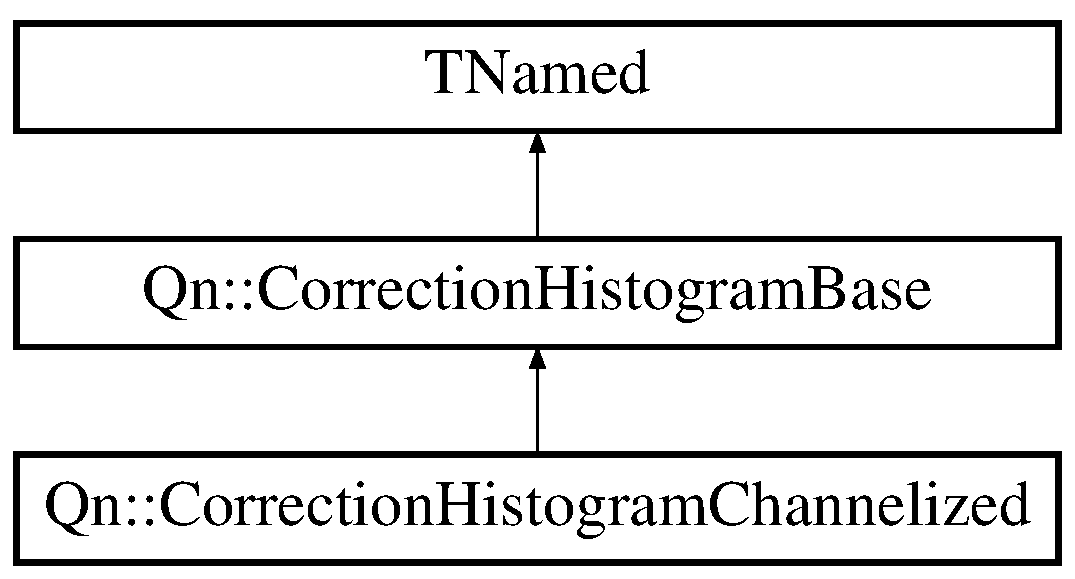
\includegraphics[height=3.000000cm]{classQn_1_1CorrectionHistogramChannelized}
\end{center}
\end{figure}
\subsection*{Public Member Functions}
\begin{DoxyCompactItemize}
\item 
\mbox{\Hypertarget{classQn_1_1CorrectionHistogramChannelized_a3f5045c2469a7eb1a34e545c2dd984ac}\label{classQn_1_1CorrectionHistogramChannelized_a3f5045c2469a7eb1a34e545c2dd984ac}} 
\mbox{\hyperlink{classQn_1_1CorrectionHistogramChannelized_a3f5045c2469a7eb1a34e545c2dd984ac}{Correction\+Histogram\+Channelized}} ()
\begin{DoxyCompactList}\small\item\em Default constructor. \end{DoxyCompactList}\item 
\mbox{\hyperlink{classQn_1_1CorrectionHistogramChannelized_a89826506f8b6aa57a6352382a25f7ddc}{Correction\+Histogram\+Channelized}} (const char $\ast$name, const char $\ast$title, \mbox{\hyperlink{classQn_1_1EventClassVariablesSet}{Event\+Class\+Variables\+Set}} \&ecvs, Int\+\_\+t n\+No\+Of\+Channels)
\item 
virtual \mbox{\hyperlink{classQn_1_1CorrectionHistogramChannelized_adc080a267712de1ca2a04349bab92b4e}{$\sim$\+Correction\+Histogram\+Channelized}} ()
\item 
Bool\+\_\+t \mbox{\hyperlink{classQn_1_1CorrectionHistogramChannelized_a3dba90ec0d5dc2a4e346d52ed980f404}{Create\+Channelized\+Histogram}} (T\+List $\ast$histogram\+List, const Bool\+\_\+t $\ast$b\+Used\+Channel)
\item 
\mbox{\Hypertarget{classQn_1_1CorrectionHistogramChannelized_ac0f40b2e62be4290571d9f55fb900058}\label{classQn_1_1CorrectionHistogramChannelized_ac0f40b2e62be4290571d9f55fb900058}} 
virtual Long64\+\_\+t \mbox{\hyperlink{classQn_1_1CorrectionHistogramChannelized_ac0f40b2e62be4290571d9f55fb900058}{Get\+Bin}} (const double $\ast$variable\+Container)
\begin{DoxyCompactList}\small\item\em wrong call for this class invoke base class behaviour \end{DoxyCompactList}\item 
virtual Long64\+\_\+t \mbox{\hyperlink{classQn_1_1CorrectionHistogramChannelized_a2491d6649af34766c3e848db8ed6e796}{Get\+Bin}} (const double $\ast$variable\+Container, Int\+\_\+t n\+Channel)
\item 
virtual Bool\+\_\+t \mbox{\hyperlink{classQn_1_1CorrectionHistogramChannelized_a12342a47b865927f259043f6816cf2e8}{Bin\+Content\+Validated}} (Long64\+\_\+t bin)
\item 
virtual Float\+\_\+t \mbox{\hyperlink{classQn_1_1CorrectionHistogramChannelized_ab398b7a1d5d9a92e183ea164882b4a53}{Get\+Bin\+Content}} (Long64\+\_\+t bin)
\item 
virtual Float\+\_\+t \mbox{\hyperlink{classQn_1_1CorrectionHistogramChannelized_a5982f9fa3ce2eb199cfdd2e518c4cb4e}{Get\+Bin\+Error}} (Long64\+\_\+t bin)
\item 
\mbox{\Hypertarget{classQn_1_1CorrectionHistogramChannelized_a9fee26c0616694e955b8785a2714b958}\label{classQn_1_1CorrectionHistogramChannelized_a9fee26c0616694e955b8785a2714b958}} 
virtual void \mbox{\hyperlink{classQn_1_1CorrectionHistogramChannelized_a9fee26c0616694e955b8785a2714b958}{Fill}} (const double $\ast$variable\+Container, Float\+\_\+t weight)
\begin{DoxyCompactList}\small\item\em wrong call for this class invoke base class behavior \end{DoxyCompactList}\item 
virtual void \mbox{\hyperlink{classQn_1_1CorrectionHistogramChannelized_a3191ab6b7b9be07eab43133ba4200ce1}{Fill}} (const double $\ast$variable\+Container, Int\+\_\+t n\+Channel, Float\+\_\+t weight)
\end{DoxyCompactItemize}
\subsection*{Additional Inherited Members}


\subsection{Constructor \& Destructor Documentation}
\mbox{\Hypertarget{classQn_1_1CorrectionHistogramChannelized_a89826506f8b6aa57a6352382a25f7ddc}\label{classQn_1_1CorrectionHistogramChannelized_a89826506f8b6aa57a6352382a25f7ddc}} 
\index{Qn\+::\+Correction\+Histogram\+Channelized@{Qn\+::\+Correction\+Histogram\+Channelized}!Correction\+Histogram\+Channelized@{Correction\+Histogram\+Channelized}}
\index{Correction\+Histogram\+Channelized@{Correction\+Histogram\+Channelized}!Qn\+::\+Correction\+Histogram\+Channelized@{Qn\+::\+Correction\+Histogram\+Channelized}}
\subsubsection{\texorpdfstring{Correction\+Histogram\+Channelized()}{CorrectionHistogramChannelized()}}
{\footnotesize\ttfamily Qn\+::\+Correction\+Histogram\+Channelized\+::\+Correction\+Histogram\+Channelized (\begin{DoxyParamCaption}\item[{const char $\ast$}]{name,  }\item[{const char $\ast$}]{title,  }\item[{\mbox{\hyperlink{classQn_1_1EventClassVariablesSet}{Event\+Class\+Variables\+Set}} \&}]{ecvs,  }\item[{Int\+\_\+t}]{n\+No\+Of\+Channels }\end{DoxyParamCaption})}

Normal constructor

Stores the set of variables that identify the different event classes passing them to its parent and prepares the object for actual histogram creation or attachment


\begin{DoxyParams}{Parameters}
{\em name} & base for the name of the histograms \\
\hline
{\em title} & base for the title of the histograms \\
\hline
{\em ecvs} & the event classes variables set \\
\hline
{\em n\+No\+Of\+Channels} & the number of channels associated \\
\hline
\end{DoxyParams}
\mbox{\Hypertarget{classQn_1_1CorrectionHistogramChannelized_adc080a267712de1ca2a04349bab92b4e}\label{classQn_1_1CorrectionHistogramChannelized_adc080a267712de1ca2a04349bab92b4e}} 
\index{Qn\+::\+Correction\+Histogram\+Channelized@{Qn\+::\+Correction\+Histogram\+Channelized}!````~Correction\+Histogram\+Channelized@{$\sim$\+Correction\+Histogram\+Channelized}}
\index{````~Correction\+Histogram\+Channelized@{$\sim$\+Correction\+Histogram\+Channelized}!Qn\+::\+Correction\+Histogram\+Channelized@{Qn\+::\+Correction\+Histogram\+Channelized}}
\subsubsection{\texorpdfstring{$\sim$\+Correction\+Histogram\+Channelized()}{~CorrectionHistogramChannelized()}}
{\footnotesize\ttfamily Qn\+::\+Correction\+Histogram\+Channelized\+::$\sim$\+Correction\+Histogram\+Channelized (\begin{DoxyParamCaption}{ }\end{DoxyParamCaption})\hspace{0.3cm}{\ttfamily [virtual]}}

Default destructor Releases the memory taken 

\subsection{Member Function Documentation}
\mbox{\Hypertarget{classQn_1_1CorrectionHistogramChannelized_a12342a47b865927f259043f6816cf2e8}\label{classQn_1_1CorrectionHistogramChannelized_a12342a47b865927f259043f6816cf2e8}} 
\index{Qn\+::\+Correction\+Histogram\+Channelized@{Qn\+::\+Correction\+Histogram\+Channelized}!Bin\+Content\+Validated@{Bin\+Content\+Validated}}
\index{Bin\+Content\+Validated@{Bin\+Content\+Validated}!Qn\+::\+Correction\+Histogram\+Channelized@{Qn\+::\+Correction\+Histogram\+Channelized}}
\subsubsection{\texorpdfstring{Bin\+Content\+Validated()}{BinContentValidated()}}
{\footnotesize\ttfamily Bool\+\_\+t Qn\+::\+Correction\+Histogram\+Channelized\+::\+Bin\+Content\+Validated (\begin{DoxyParamCaption}\item[{Long64\+\_\+t}]{bin }\end{DoxyParamCaption})\hspace{0.3cm}{\ttfamily [virtual]}}

Check the validity of the content of the passed bin This kind of histograms cannot validate the bin content so, it is always valid. 
\begin{DoxyParams}{Parameters}
{\em bin} & the bin to check its content validity \\
\hline
\end{DoxyParams}
\begin{DoxyReturn}{Returns}
k\+T\+R\+UE if the content is valid k\+F\+A\+L\+SE otherwise 
\end{DoxyReturn}


Implements \mbox{\hyperlink{classQn_1_1CorrectionHistogramBase_a4db2c92ceaffefaa91475a721612d80d}{Qn\+::\+Correction\+Histogram\+Base}}.

\mbox{\Hypertarget{classQn_1_1CorrectionHistogramChannelized_a3dba90ec0d5dc2a4e346d52ed980f404}\label{classQn_1_1CorrectionHistogramChannelized_a3dba90ec0d5dc2a4e346d52ed980f404}} 
\index{Qn\+::\+Correction\+Histogram\+Channelized@{Qn\+::\+Correction\+Histogram\+Channelized}!Create\+Channelized\+Histogram@{Create\+Channelized\+Histogram}}
\index{Create\+Channelized\+Histogram@{Create\+Channelized\+Histogram}!Qn\+::\+Correction\+Histogram\+Channelized@{Qn\+::\+Correction\+Histogram\+Channelized}}
\subsubsection{\texorpdfstring{Create\+Channelized\+Histogram()}{CreateChannelizedHistogram()}}
{\footnotesize\ttfamily Bool\+\_\+t Qn\+::\+Correction\+Histogram\+Channelized\+::\+Create\+Channelized\+Histogram (\begin{DoxyParamCaption}\item[{T\+List $\ast$}]{histogram\+List,  }\item[{const Bool\+\_\+t $\ast$}]{b\+Used\+Channel }\end{DoxyParamCaption})}

Creates the support histogram for the channelize histogram function

Based in the event classes variables set in the parent class and the channel information passed as parameters the values multidimensional histogram is created.

The histogram is added to the passed histogram list

The actual number of channels is stored and a mask from external channel number to histogram channel number. If b\+Used\+Channel is N\+U\+LL all channels within f\+No\+Of\+Channels are assigned to this profile. 
\begin{DoxyParams}{Parameters}
{\em histogram\+List} & list where the histograms have to be added \\
\hline
{\em b\+Used\+Channel} & array of booleans one per each channel \\
\hline
\end{DoxyParams}
\begin{DoxyReturn}{Returns}
true if properly created 
\end{DoxyReturn}
\mbox{\Hypertarget{classQn_1_1CorrectionHistogramChannelized_a3191ab6b7b9be07eab43133ba4200ce1}\label{classQn_1_1CorrectionHistogramChannelized_a3191ab6b7b9be07eab43133ba4200ce1}} 
\index{Qn\+::\+Correction\+Histogram\+Channelized@{Qn\+::\+Correction\+Histogram\+Channelized}!Fill@{Fill}}
\index{Fill@{Fill}!Qn\+::\+Correction\+Histogram\+Channelized@{Qn\+::\+Correction\+Histogram\+Channelized}}
\subsubsection{\texorpdfstring{Fill()}{Fill()}}
{\footnotesize\ttfamily void Qn\+::\+Correction\+Histogram\+Channelized\+::\+Fill (\begin{DoxyParamCaption}\item[{const double $\ast$}]{variable\+Container,  }\item[{Int\+\_\+t}]{n\+Channel,  }\item[{Float\+\_\+t}]{weight }\end{DoxyParamCaption})\hspace{0.3cm}{\ttfamily [virtual]}}

Fills the histogram

The involved bin is computed according to the current variables content and the passed external channel number. The bin is then increased by the given weight.


\begin{DoxyParams}{Parameters}
{\em variable\+Container} & the current variables content addressed by var Id \\
\hline
{\em n\+Channel} & the interested external channel number \\
\hline
{\em weight} & the increment in the bin content \\
\hline
\end{DoxyParams}


Reimplemented from \mbox{\hyperlink{classQn_1_1CorrectionHistogramBase_ae94b20c7d396f5b179fb11d84d764c09}{Qn\+::\+Correction\+Histogram\+Base}}.

\mbox{\Hypertarget{classQn_1_1CorrectionHistogramChannelized_a2491d6649af34766c3e848db8ed6e796}\label{classQn_1_1CorrectionHistogramChannelized_a2491d6649af34766c3e848db8ed6e796}} 
\index{Qn\+::\+Correction\+Histogram\+Channelized@{Qn\+::\+Correction\+Histogram\+Channelized}!Get\+Bin@{Get\+Bin}}
\index{Get\+Bin@{Get\+Bin}!Qn\+::\+Correction\+Histogram\+Channelized@{Qn\+::\+Correction\+Histogram\+Channelized}}
\subsubsection{\texorpdfstring{Get\+Bin()}{GetBin()}}
{\footnotesize\ttfamily Long64\+\_\+t Qn\+::\+Correction\+Histogram\+Channelized\+::\+Get\+Bin (\begin{DoxyParamCaption}\item[{const double $\ast$}]{variable\+Container,  }\item[{Int\+\_\+t}]{n\+Channel }\end{DoxyParamCaption})\hspace{0.3cm}{\ttfamily [virtual]}}

Get the bin number for the current variable content and passed channel

The bin number identifies the event class the current variable content points to under the passed channel.


\begin{DoxyParams}{Parameters}
{\em variable\+Container} & the current variables content addressed by var Id \\
\hline
{\em n\+Channel} & the interested external channel number \\
\hline
\end{DoxyParams}
\begin{DoxyReturn}{Returns}
the associated bin to the current variables content 
\end{DoxyReturn}


Reimplemented from \mbox{\hyperlink{classQn_1_1CorrectionHistogramBase_acfde166908e4da950470841f21f87fb9}{Qn\+::\+Correction\+Histogram\+Base}}.

\mbox{\Hypertarget{classQn_1_1CorrectionHistogramChannelized_ab398b7a1d5d9a92e183ea164882b4a53}\label{classQn_1_1CorrectionHistogramChannelized_ab398b7a1d5d9a92e183ea164882b4a53}} 
\index{Qn\+::\+Correction\+Histogram\+Channelized@{Qn\+::\+Correction\+Histogram\+Channelized}!Get\+Bin\+Content@{Get\+Bin\+Content}}
\index{Get\+Bin\+Content@{Get\+Bin\+Content}!Qn\+::\+Correction\+Histogram\+Channelized@{Qn\+::\+Correction\+Histogram\+Channelized}}
\subsubsection{\texorpdfstring{Get\+Bin\+Content()}{GetBinContent()}}
{\footnotesize\ttfamily Float\+\_\+t Qn\+::\+Correction\+Histogram\+Channelized\+::\+Get\+Bin\+Content (\begin{DoxyParamCaption}\item[{Long64\+\_\+t}]{bin }\end{DoxyParamCaption})\hspace{0.3cm}{\ttfamily [virtual]}}

Get the bin content for the passed bin number

The bin number identifies a desired event class whose content is requested.


\begin{DoxyParams}{Parameters}
{\em bin} & the interested bin number \\
\hline
\end{DoxyParams}
\begin{DoxyReturn}{Returns}
the bin number content 
\end{DoxyReturn}


Reimplemented from \mbox{\hyperlink{classQn_1_1CorrectionHistogramBase_a9e4e745a6f4cbebf5b9277d6d63bc9c7}{Qn\+::\+Correction\+Histogram\+Base}}.

\mbox{\Hypertarget{classQn_1_1CorrectionHistogramChannelized_a5982f9fa3ce2eb199cfdd2e518c4cb4e}\label{classQn_1_1CorrectionHistogramChannelized_a5982f9fa3ce2eb199cfdd2e518c4cb4e}} 
\index{Qn\+::\+Correction\+Histogram\+Channelized@{Qn\+::\+Correction\+Histogram\+Channelized}!Get\+Bin\+Error@{Get\+Bin\+Error}}
\index{Get\+Bin\+Error@{Get\+Bin\+Error}!Qn\+::\+Correction\+Histogram\+Channelized@{Qn\+::\+Correction\+Histogram\+Channelized}}
\subsubsection{\texorpdfstring{Get\+Bin\+Error()}{GetBinError()}}
{\footnotesize\ttfamily Float\+\_\+t Qn\+::\+Correction\+Histogram\+Channelized\+::\+Get\+Bin\+Error (\begin{DoxyParamCaption}\item[{Long64\+\_\+t}]{bin }\end{DoxyParamCaption})\hspace{0.3cm}{\ttfamily [virtual]}}

Get the bin content error for the passed bin number

The bin number identifies a desired event class whose content error is requested.


\begin{DoxyParams}{Parameters}
{\em bin} & the interested bin number \\
\hline
\end{DoxyParams}
\begin{DoxyReturn}{Returns}
the bin number content error 
\end{DoxyReturn}


Reimplemented from \mbox{\hyperlink{classQn_1_1CorrectionHistogramBase_a50a7dd4c5bbe5e4d0e405365c2a9104d}{Qn\+::\+Correction\+Histogram\+Base}}.



The documentation for this class was generated from the following files\+:\begin{DoxyCompactItemize}
\item 
D\+T\+\_\+\+Flow/\+Qn\+Corrections/include/Correction\+Histogram\+Channelized.\+h\item 
D\+T\+\_\+\+Flow/\+Qn\+Corrections/Correction\+Histogram\+Channelized.\+cpp\end{DoxyCompactItemize}

\hypertarget{classQn_1_1CorrectionHistogramChannelizedSparse}{}\section{Qn\+:\+:Correction\+Histogram\+Channelized\+Sparse Class Reference}
\label{classQn_1_1CorrectionHistogramChannelizedSparse}\index{Qn\+::\+Correction\+Histogram\+Channelized\+Sparse@{Qn\+::\+Correction\+Histogram\+Channelized\+Sparse}}
Inheritance diagram for Qn\+:\+:Correction\+Histogram\+Channelized\+Sparse\+:\begin{figure}[H]
\begin{center}
\leavevmode
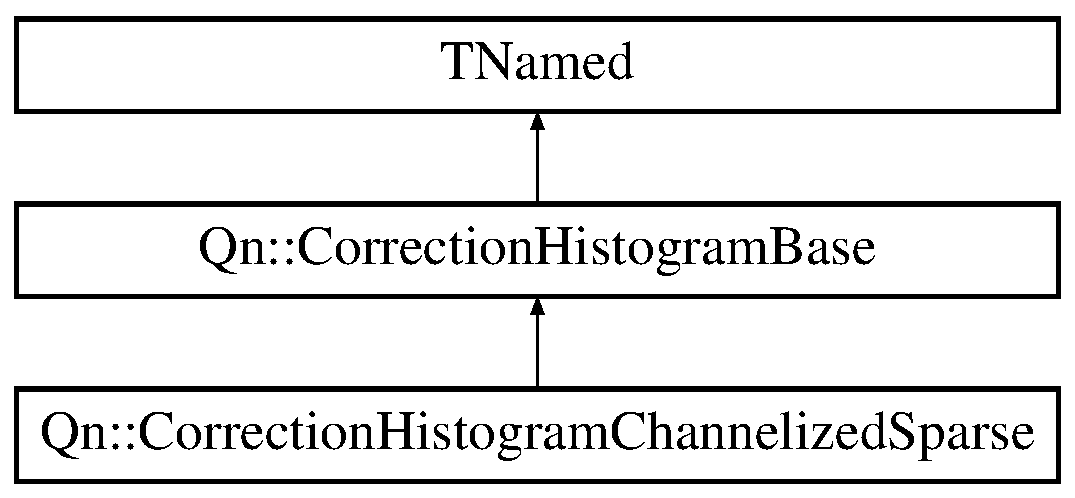
\includegraphics[height=3.000000cm]{classQn_1_1CorrectionHistogramChannelizedSparse}
\end{center}
\end{figure}
\subsection*{Public Member Functions}
\begin{DoxyCompactItemize}
\item 
\mbox{\Hypertarget{classQn_1_1CorrectionHistogramChannelizedSparse_a623217a23dea7235cb4e03ad3f401f29}\label{classQn_1_1CorrectionHistogramChannelizedSparse_a623217a23dea7235cb4e03ad3f401f29}} 
\mbox{\hyperlink{classQn_1_1CorrectionHistogramChannelizedSparse_a623217a23dea7235cb4e03ad3f401f29}{Correction\+Histogram\+Channelized\+Sparse}} ()
\begin{DoxyCompactList}\small\item\em Default constructor. \end{DoxyCompactList}\item 
\mbox{\hyperlink{classQn_1_1CorrectionHistogramChannelizedSparse_a018a19416ce8241d58db9d611cfcc1ac}{Correction\+Histogram\+Channelized\+Sparse}} (const char $\ast$name, const char $\ast$title, \mbox{\hyperlink{classQn_1_1EventClassVariablesSet}{Event\+Class\+Variables\+Set}} \&ecvs, Int\+\_\+t n\+No\+Of\+Channels)
\item 
virtual \mbox{\hyperlink{classQn_1_1CorrectionHistogramChannelizedSparse_a7d0b5bd1526fa4c8464aed5aa15ca208}{$\sim$\+Correction\+Histogram\+Channelized\+Sparse}} ()
\item 
Bool\+\_\+t \mbox{\hyperlink{classQn_1_1CorrectionHistogramChannelizedSparse_af17e3d8de269e5e3f620ccc5896b06b3}{Create\+Channelized\+Histogram}} (T\+List $\ast$histogram\+List, const Bool\+\_\+t $\ast$b\+Used\+Channel)
\item 
\mbox{\Hypertarget{classQn_1_1CorrectionHistogramChannelizedSparse_aadda1224f18ee306c731f78855c3b3b0}\label{classQn_1_1CorrectionHistogramChannelizedSparse_aadda1224f18ee306c731f78855c3b3b0}} 
virtual Long64\+\_\+t \mbox{\hyperlink{classQn_1_1CorrectionHistogramChannelizedSparse_aadda1224f18ee306c731f78855c3b3b0}{Get\+Bin}} (const double $\ast$variable\+Container)
\begin{DoxyCompactList}\small\item\em wrong call for this class invoke base class behaviour \end{DoxyCompactList}\item 
virtual Long64\+\_\+t \mbox{\hyperlink{classQn_1_1CorrectionHistogramChannelizedSparse_a02df93ea7f488eab8cd0c781c1c71808}{Get\+Bin}} (const double $\ast$variable\+Container, Int\+\_\+t n\+Channel)
\item 
virtual Bool\+\_\+t \mbox{\hyperlink{classQn_1_1CorrectionHistogramChannelizedSparse_a46f0289fe5ddd088356679486d8376d6}{Bin\+Content\+Validated}} (Long64\+\_\+t bin)
\item 
virtual Float\+\_\+t \mbox{\hyperlink{classQn_1_1CorrectionHistogramChannelizedSparse_a247aa9d6cadd6c5373ed4cf0cde8b719}{Get\+Bin\+Content}} (Long64\+\_\+t bin)
\item 
virtual Float\+\_\+t \mbox{\hyperlink{classQn_1_1CorrectionHistogramChannelizedSparse_a1b683c6af5cf7dea4d0ee9fa367e0d09}{Get\+Bin\+Error}} (Long64\+\_\+t bin)
\item 
\mbox{\Hypertarget{classQn_1_1CorrectionHistogramChannelizedSparse_adcd90b4926b6932cd9b50a9790d172b1}\label{classQn_1_1CorrectionHistogramChannelizedSparse_adcd90b4926b6932cd9b50a9790d172b1}} 
virtual void \mbox{\hyperlink{classQn_1_1CorrectionHistogramChannelizedSparse_adcd90b4926b6932cd9b50a9790d172b1}{Fill}} (const double $\ast$variable\+Container, Float\+\_\+t weight)
\begin{DoxyCompactList}\small\item\em wrong call for this class invoke base class behavior \end{DoxyCompactList}\item 
virtual void \mbox{\hyperlink{classQn_1_1CorrectionHistogramChannelizedSparse_a11c6c6d5b037fdf9c4f03d2f54e7a526}{Fill}} (const double $\ast$variable\+Container, Int\+\_\+t n\+Channel, Float\+\_\+t weight)
\end{DoxyCompactItemize}
\subsection*{Additional Inherited Members}


\subsection{Constructor \& Destructor Documentation}
\mbox{\Hypertarget{classQn_1_1CorrectionHistogramChannelizedSparse_a018a19416ce8241d58db9d611cfcc1ac}\label{classQn_1_1CorrectionHistogramChannelizedSparse_a018a19416ce8241d58db9d611cfcc1ac}} 
\index{Qn\+::\+Correction\+Histogram\+Channelized\+Sparse@{Qn\+::\+Correction\+Histogram\+Channelized\+Sparse}!Correction\+Histogram\+Channelized\+Sparse@{Correction\+Histogram\+Channelized\+Sparse}}
\index{Correction\+Histogram\+Channelized\+Sparse@{Correction\+Histogram\+Channelized\+Sparse}!Qn\+::\+Correction\+Histogram\+Channelized\+Sparse@{Qn\+::\+Correction\+Histogram\+Channelized\+Sparse}}
\subsubsection{\texorpdfstring{Correction\+Histogram\+Channelized\+Sparse()}{CorrectionHistogramChannelizedSparse()}}
{\footnotesize\ttfamily Qn\+::\+Correction\+Histogram\+Channelized\+Sparse\+::\+Correction\+Histogram\+Channelized\+Sparse (\begin{DoxyParamCaption}\item[{const char $\ast$}]{name,  }\item[{const char $\ast$}]{title,  }\item[{\mbox{\hyperlink{classQn_1_1EventClassVariablesSet}{Event\+Class\+Variables\+Set}} \&}]{ecvs,  }\item[{Int\+\_\+t}]{n\+No\+Of\+Channels }\end{DoxyParamCaption})}

Normal constructor

Stores the set of variables that identify the different event classes passing them to its parent and prepares the object for actual histogram creation or attachment


\begin{DoxyParams}{Parameters}
{\em name} & base for the name of the histograms \\
\hline
{\em title} & base for the title of the histograms \\
\hline
{\em ecvs} & the event classes variables set \\
\hline
{\em n\+No\+Of\+Channels} & the number of channels associated \\
\hline
\end{DoxyParams}
\mbox{\Hypertarget{classQn_1_1CorrectionHistogramChannelizedSparse_a7d0b5bd1526fa4c8464aed5aa15ca208}\label{classQn_1_1CorrectionHistogramChannelizedSparse_a7d0b5bd1526fa4c8464aed5aa15ca208}} 
\index{Qn\+::\+Correction\+Histogram\+Channelized\+Sparse@{Qn\+::\+Correction\+Histogram\+Channelized\+Sparse}!````~Correction\+Histogram\+Channelized\+Sparse@{$\sim$\+Correction\+Histogram\+Channelized\+Sparse}}
\index{````~Correction\+Histogram\+Channelized\+Sparse@{$\sim$\+Correction\+Histogram\+Channelized\+Sparse}!Qn\+::\+Correction\+Histogram\+Channelized\+Sparse@{Qn\+::\+Correction\+Histogram\+Channelized\+Sparse}}
\subsubsection{\texorpdfstring{$\sim$\+Correction\+Histogram\+Channelized\+Sparse()}{~CorrectionHistogramChannelizedSparse()}}
{\footnotesize\ttfamily Qn\+::\+Correction\+Histogram\+Channelized\+Sparse\+::$\sim$\+Correction\+Histogram\+Channelized\+Sparse (\begin{DoxyParamCaption}{ }\end{DoxyParamCaption})\hspace{0.3cm}{\ttfamily [virtual]}}

Default destructor Releases the memory taken 

\subsection{Member Function Documentation}
\mbox{\Hypertarget{classQn_1_1CorrectionHistogramChannelizedSparse_a46f0289fe5ddd088356679486d8376d6}\label{classQn_1_1CorrectionHistogramChannelizedSparse_a46f0289fe5ddd088356679486d8376d6}} 
\index{Qn\+::\+Correction\+Histogram\+Channelized\+Sparse@{Qn\+::\+Correction\+Histogram\+Channelized\+Sparse}!Bin\+Content\+Validated@{Bin\+Content\+Validated}}
\index{Bin\+Content\+Validated@{Bin\+Content\+Validated}!Qn\+::\+Correction\+Histogram\+Channelized\+Sparse@{Qn\+::\+Correction\+Histogram\+Channelized\+Sparse}}
\subsubsection{\texorpdfstring{Bin\+Content\+Validated()}{BinContentValidated()}}
{\footnotesize\ttfamily Bool\+\_\+t Qn\+::\+Correction\+Histogram\+Channelized\+Sparse\+::\+Bin\+Content\+Validated (\begin{DoxyParamCaption}\item[{Long64\+\_\+t}]{bin }\end{DoxyParamCaption})\hspace{0.3cm}{\ttfamily [virtual]}}

Check the validity of the content of the passed bin This kind of histograms cannot validate the bin content so, it is always valid. 
\begin{DoxyParams}{Parameters}
{\em bin} & the bin to check its content validity \\
\hline
\end{DoxyParams}
\begin{DoxyReturn}{Returns}
k\+T\+R\+UE if the content is valid k\+F\+A\+L\+SE otherwise 
\end{DoxyReturn}


Implements \mbox{\hyperlink{classQn_1_1CorrectionHistogramBase_a4db2c92ceaffefaa91475a721612d80d}{Qn\+::\+Correction\+Histogram\+Base}}.

\mbox{\Hypertarget{classQn_1_1CorrectionHistogramChannelizedSparse_af17e3d8de269e5e3f620ccc5896b06b3}\label{classQn_1_1CorrectionHistogramChannelizedSparse_af17e3d8de269e5e3f620ccc5896b06b3}} 
\index{Qn\+::\+Correction\+Histogram\+Channelized\+Sparse@{Qn\+::\+Correction\+Histogram\+Channelized\+Sparse}!Create\+Channelized\+Histogram@{Create\+Channelized\+Histogram}}
\index{Create\+Channelized\+Histogram@{Create\+Channelized\+Histogram}!Qn\+::\+Correction\+Histogram\+Channelized\+Sparse@{Qn\+::\+Correction\+Histogram\+Channelized\+Sparse}}
\subsubsection{\texorpdfstring{Create\+Channelized\+Histogram()}{CreateChannelizedHistogram()}}
{\footnotesize\ttfamily Bool\+\_\+t Qn\+::\+Correction\+Histogram\+Channelized\+Sparse\+::\+Create\+Channelized\+Histogram (\begin{DoxyParamCaption}\item[{T\+List $\ast$}]{histogram\+List,  }\item[{const Bool\+\_\+t $\ast$}]{b\+Used\+Channel }\end{DoxyParamCaption})}

Creates the support histogram for the channelize histogram function

Based in the event classes variables set in the parent class and the channel information passed as parameters the values multidimensional histogram is created.

The histogram is added to the passed histogram list

The actual number of channels is stored and a mask from external channel number to histogram channel number. If b\+Used\+Channel is N\+U\+LL all channels within f\+No\+Of\+Channels are assigned to this profile. 
\begin{DoxyParams}{Parameters}
{\em histogram\+List} & list where the histograms have to be added \\
\hline
{\em b\+Used\+Channel} & array of booleans one per each channel \\
\hline
\end{DoxyParams}
\begin{DoxyReturn}{Returns}
true if properly created 
\end{DoxyReturn}
\mbox{\Hypertarget{classQn_1_1CorrectionHistogramChannelizedSparse_a11c6c6d5b037fdf9c4f03d2f54e7a526}\label{classQn_1_1CorrectionHistogramChannelizedSparse_a11c6c6d5b037fdf9c4f03d2f54e7a526}} 
\index{Qn\+::\+Correction\+Histogram\+Channelized\+Sparse@{Qn\+::\+Correction\+Histogram\+Channelized\+Sparse}!Fill@{Fill}}
\index{Fill@{Fill}!Qn\+::\+Correction\+Histogram\+Channelized\+Sparse@{Qn\+::\+Correction\+Histogram\+Channelized\+Sparse}}
\subsubsection{\texorpdfstring{Fill()}{Fill()}}
{\footnotesize\ttfamily void Qn\+::\+Correction\+Histogram\+Channelized\+Sparse\+::\+Fill (\begin{DoxyParamCaption}\item[{const double $\ast$}]{variable\+Container,  }\item[{Int\+\_\+t}]{n\+Channel,  }\item[{Float\+\_\+t}]{weight }\end{DoxyParamCaption})\hspace{0.3cm}{\ttfamily [virtual]}}

Fills the histogram

The involved bin is computed according to the current variables content and the passed external channel number. The bin is then increased by the given weight.


\begin{DoxyParams}{Parameters}
{\em variable\+Container} & the current variables content addressed by var Id \\
\hline
{\em n\+Channel} & the interested external channel number \\
\hline
{\em weight} & the increment in the bin content \\
\hline
\end{DoxyParams}


Reimplemented from \mbox{\hyperlink{classQn_1_1CorrectionHistogramBase_ae94b20c7d396f5b179fb11d84d764c09}{Qn\+::\+Correction\+Histogram\+Base}}.

\mbox{\Hypertarget{classQn_1_1CorrectionHistogramChannelizedSparse_a02df93ea7f488eab8cd0c781c1c71808}\label{classQn_1_1CorrectionHistogramChannelizedSparse_a02df93ea7f488eab8cd0c781c1c71808}} 
\index{Qn\+::\+Correction\+Histogram\+Channelized\+Sparse@{Qn\+::\+Correction\+Histogram\+Channelized\+Sparse}!Get\+Bin@{Get\+Bin}}
\index{Get\+Bin@{Get\+Bin}!Qn\+::\+Correction\+Histogram\+Channelized\+Sparse@{Qn\+::\+Correction\+Histogram\+Channelized\+Sparse}}
\subsubsection{\texorpdfstring{Get\+Bin()}{GetBin()}}
{\footnotesize\ttfamily Long64\+\_\+t Qn\+::\+Correction\+Histogram\+Channelized\+Sparse\+::\+Get\+Bin (\begin{DoxyParamCaption}\item[{const double $\ast$}]{variable\+Container,  }\item[{Int\+\_\+t}]{n\+Channel }\end{DoxyParamCaption})\hspace{0.3cm}{\ttfamily [virtual]}}

Get the bin number for the current variable content and passed channel

The bin number identifies the event class the current variable content points to under the passed channel.


\begin{DoxyParams}{Parameters}
{\em variable\+Container} & the current variables content addressed by var Id \\
\hline
{\em n\+Channel} & the interested external channel number \\
\hline
\end{DoxyParams}
\begin{DoxyReturn}{Returns}
the associated bin to the current variables content 
\end{DoxyReturn}


Reimplemented from \mbox{\hyperlink{classQn_1_1CorrectionHistogramBase_acfde166908e4da950470841f21f87fb9}{Qn\+::\+Correction\+Histogram\+Base}}.

\mbox{\Hypertarget{classQn_1_1CorrectionHistogramChannelizedSparse_a247aa9d6cadd6c5373ed4cf0cde8b719}\label{classQn_1_1CorrectionHistogramChannelizedSparse_a247aa9d6cadd6c5373ed4cf0cde8b719}} 
\index{Qn\+::\+Correction\+Histogram\+Channelized\+Sparse@{Qn\+::\+Correction\+Histogram\+Channelized\+Sparse}!Get\+Bin\+Content@{Get\+Bin\+Content}}
\index{Get\+Bin\+Content@{Get\+Bin\+Content}!Qn\+::\+Correction\+Histogram\+Channelized\+Sparse@{Qn\+::\+Correction\+Histogram\+Channelized\+Sparse}}
\subsubsection{\texorpdfstring{Get\+Bin\+Content()}{GetBinContent()}}
{\footnotesize\ttfamily Float\+\_\+t Qn\+::\+Correction\+Histogram\+Channelized\+Sparse\+::\+Get\+Bin\+Content (\begin{DoxyParamCaption}\item[{Long64\+\_\+t}]{bin }\end{DoxyParamCaption})\hspace{0.3cm}{\ttfamily [virtual]}}

Get the bin content for the passed bin number

The bin number identifies a desired event class whose content is requested.


\begin{DoxyParams}{Parameters}
{\em bin} & the interested bin number \\
\hline
\end{DoxyParams}
\begin{DoxyReturn}{Returns}
the bin number content 
\end{DoxyReturn}


Reimplemented from \mbox{\hyperlink{classQn_1_1CorrectionHistogramBase_a9e4e745a6f4cbebf5b9277d6d63bc9c7}{Qn\+::\+Correction\+Histogram\+Base}}.

\mbox{\Hypertarget{classQn_1_1CorrectionHistogramChannelizedSparse_a1b683c6af5cf7dea4d0ee9fa367e0d09}\label{classQn_1_1CorrectionHistogramChannelizedSparse_a1b683c6af5cf7dea4d0ee9fa367e0d09}} 
\index{Qn\+::\+Correction\+Histogram\+Channelized\+Sparse@{Qn\+::\+Correction\+Histogram\+Channelized\+Sparse}!Get\+Bin\+Error@{Get\+Bin\+Error}}
\index{Get\+Bin\+Error@{Get\+Bin\+Error}!Qn\+::\+Correction\+Histogram\+Channelized\+Sparse@{Qn\+::\+Correction\+Histogram\+Channelized\+Sparse}}
\subsubsection{\texorpdfstring{Get\+Bin\+Error()}{GetBinError()}}
{\footnotesize\ttfamily Float\+\_\+t Qn\+::\+Correction\+Histogram\+Channelized\+Sparse\+::\+Get\+Bin\+Error (\begin{DoxyParamCaption}\item[{Long64\+\_\+t}]{bin }\end{DoxyParamCaption})\hspace{0.3cm}{\ttfamily [virtual]}}

Get the bin content error for the passed bin number

The bin number identifies a desired event class whose content error is requested.


\begin{DoxyParams}{Parameters}
{\em bin} & the interested bin number \\
\hline
\end{DoxyParams}
\begin{DoxyReturn}{Returns}
the bin number content error 
\end{DoxyReturn}


Reimplemented from \mbox{\hyperlink{classQn_1_1CorrectionHistogramBase_a50a7dd4c5bbe5e4d0e405365c2a9104d}{Qn\+::\+Correction\+Histogram\+Base}}.



The documentation for this class was generated from the following files\+:\begin{DoxyCompactItemize}
\item 
D\+T\+\_\+\+Flow/\+Qn\+Corrections/include/Correction\+Histogram\+Channelized\+Sparse.\+h\item 
D\+T\+\_\+\+Flow/\+Qn\+Corrections/Correction\+Histogram\+Channelized\+Sparse.\+cpp\end{DoxyCompactItemize}

\hypertarget{classQn_1_1CorrectionHistogramSparse}{}\section{Qn\+:\+:Correction\+Histogram\+Sparse Class Reference}
\label{classQn_1_1CorrectionHistogramSparse}\index{Qn\+::\+Correction\+Histogram\+Sparse@{Qn\+::\+Correction\+Histogram\+Sparse}}
Inheritance diagram for Qn\+:\+:Correction\+Histogram\+Sparse\+:\begin{figure}[H]
\begin{center}
\leavevmode
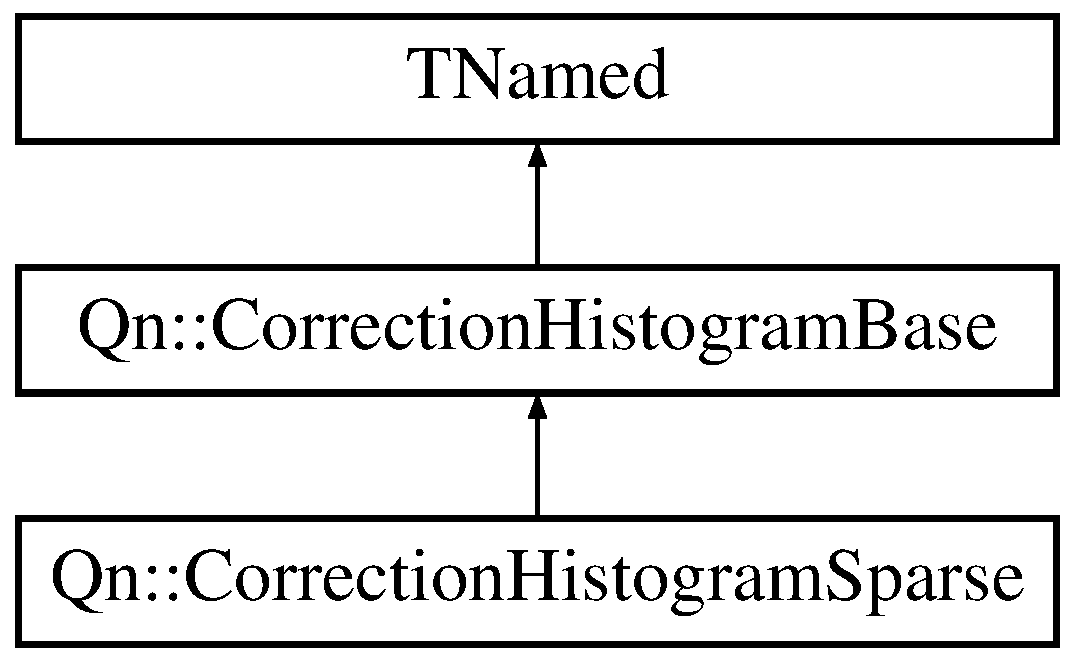
\includegraphics[height=3.000000cm]{classQn_1_1CorrectionHistogramSparse}
\end{center}
\end{figure}
\subsection*{Public Member Functions}
\begin{DoxyCompactItemize}
\item 
\mbox{\Hypertarget{classQn_1_1CorrectionHistogramSparse_ac3030ab0d31967648b7d1ad11423c931}\label{classQn_1_1CorrectionHistogramSparse_ac3030ab0d31967648b7d1ad11423c931}} 
\mbox{\hyperlink{classQn_1_1CorrectionHistogramSparse_ac3030ab0d31967648b7d1ad11423c931}{Correction\+Histogram\+Sparse}} ()
\begin{DoxyCompactList}\small\item\em Default constructor. \end{DoxyCompactList}\item 
\mbox{\hyperlink{classQn_1_1CorrectionHistogramSparse_a0399954f4572a32e62d70a7ea0fc7e17}{Correction\+Histogram\+Sparse}} (const char $\ast$name, const char $\ast$title, \mbox{\hyperlink{classQn_1_1EventClassVariablesSet}{Event\+Class\+Variables\+Set}} \&ecvs)
\item 
virtual \mbox{\hyperlink{classQn_1_1CorrectionHistogramSparse_aa8f2252efa1bdf5a4fd166aaf0f4c6ea}{$\sim$\+Correction\+Histogram\+Sparse}} ()
\item 
Bool\+\_\+t \mbox{\hyperlink{classQn_1_1CorrectionHistogramSparse_a53ee93b38933721305a26860324a03ea}{Create\+Histogram}} (T\+List $\ast$histogram\+List)
\item 
virtual Long64\+\_\+t \mbox{\hyperlink{classQn_1_1CorrectionHistogramSparse_aea9b7cdd8ad93d5fb14c00b20848dcdc}{Get\+Bin}} (const double $\ast$variable\+Container)
\item 
\mbox{\Hypertarget{classQn_1_1CorrectionHistogramSparse_a1b0edb414fa4594421f44a793b0fc87a}\label{classQn_1_1CorrectionHistogramSparse_a1b0edb414fa4594421f44a793b0fc87a}} 
virtual Long64\+\_\+t \mbox{\hyperlink{classQn_1_1CorrectionHistogramSparse_a1b0edb414fa4594421f44a793b0fc87a}{Get\+Bin}} (const double $\ast$variable\+Container, Int\+\_\+t n\+Channel)
\begin{DoxyCompactList}\small\item\em wrong call for this class invoke base class behaviour \end{DoxyCompactList}\item 
virtual Bool\+\_\+t \mbox{\hyperlink{classQn_1_1CorrectionHistogramSparse_a0af98e0b06c550ed265494e1f3089779}{Bin\+Content\+Validated}} (Long64\+\_\+t bin)
\item 
virtual Float\+\_\+t \mbox{\hyperlink{classQn_1_1CorrectionHistogramSparse_a43954a12a3f97e20a1934f18ec4edecd}{Get\+Bin\+Content}} (Long64\+\_\+t bin)
\item 
virtual Float\+\_\+t \mbox{\hyperlink{classQn_1_1CorrectionHistogramSparse_a9b678b088ca0b21e6deb18d66ac44c2d}{Get\+Bin\+Error}} (Long64\+\_\+t bin)
\item 
virtual void \mbox{\hyperlink{classQn_1_1CorrectionHistogramSparse_a0bb5a6f7772532ed7a174cc688cf5b92}{Fill}} (const double $\ast$variable\+Container, Float\+\_\+t weight)
\item 
\mbox{\Hypertarget{classQn_1_1CorrectionHistogramSparse_ac6669127f178e1a7c7cbf149576371bd}\label{classQn_1_1CorrectionHistogramSparse_ac6669127f178e1a7c7cbf149576371bd}} 
virtual void \mbox{\hyperlink{classQn_1_1CorrectionHistogramSparse_ac6669127f178e1a7c7cbf149576371bd}{Fill}} (const double $\ast$variable\+Container, Int\+\_\+t n\+Channel, Float\+\_\+t weight)
\begin{DoxyCompactList}\small\item\em wrong call for this class invoke base class behavior \end{DoxyCompactList}\end{DoxyCompactItemize}
\subsection*{Additional Inherited Members}


\subsection{Constructor \& Destructor Documentation}
\mbox{\Hypertarget{classQn_1_1CorrectionHistogramSparse_a0399954f4572a32e62d70a7ea0fc7e17}\label{classQn_1_1CorrectionHistogramSparse_a0399954f4572a32e62d70a7ea0fc7e17}} 
\index{Qn\+::\+Correction\+Histogram\+Sparse@{Qn\+::\+Correction\+Histogram\+Sparse}!Correction\+Histogram\+Sparse@{Correction\+Histogram\+Sparse}}
\index{Correction\+Histogram\+Sparse@{Correction\+Histogram\+Sparse}!Qn\+::\+Correction\+Histogram\+Sparse@{Qn\+::\+Correction\+Histogram\+Sparse}}
\subsubsection{\texorpdfstring{Correction\+Histogram\+Sparse()}{CorrectionHistogramSparse()}}
{\footnotesize\ttfamily Qn\+::\+Correction\+Histogram\+Sparse\+::\+Correction\+Histogram\+Sparse (\begin{DoxyParamCaption}\item[{const char $\ast$}]{name,  }\item[{const char $\ast$}]{title,  }\item[{\mbox{\hyperlink{classQn_1_1EventClassVariablesSet}{Event\+Class\+Variables\+Set}} \&}]{ecvs }\end{DoxyParamCaption})}

Normal constructor

Stores the set of variables that identify the different event classes passing them to its parent and prepares the object for actual histogram creation or attachment


\begin{DoxyParams}{Parameters}
{\em name} & base for the name of the histograms \\
\hline
{\em title} & base for the title of the histograms \\
\hline
{\em ecvs} & the event classes variables set \\
\hline
\end{DoxyParams}
\mbox{\Hypertarget{classQn_1_1CorrectionHistogramSparse_aa8f2252efa1bdf5a4fd166aaf0f4c6ea}\label{classQn_1_1CorrectionHistogramSparse_aa8f2252efa1bdf5a4fd166aaf0f4c6ea}} 
\index{Qn\+::\+Correction\+Histogram\+Sparse@{Qn\+::\+Correction\+Histogram\+Sparse}!````~Correction\+Histogram\+Sparse@{$\sim$\+Correction\+Histogram\+Sparse}}
\index{````~Correction\+Histogram\+Sparse@{$\sim$\+Correction\+Histogram\+Sparse}!Qn\+::\+Correction\+Histogram\+Sparse@{Qn\+::\+Correction\+Histogram\+Sparse}}
\subsubsection{\texorpdfstring{$\sim$\+Correction\+Histogram\+Sparse()}{~CorrectionHistogramSparse()}}
{\footnotesize\ttfamily Qn\+::\+Correction\+Histogram\+Sparse\+::$\sim$\+Correction\+Histogram\+Sparse (\begin{DoxyParamCaption}{ }\end{DoxyParamCaption})\hspace{0.3cm}{\ttfamily [virtual]}}

Default destructor Releases the memory taken 

\subsection{Member Function Documentation}
\mbox{\Hypertarget{classQn_1_1CorrectionHistogramSparse_a0af98e0b06c550ed265494e1f3089779}\label{classQn_1_1CorrectionHistogramSparse_a0af98e0b06c550ed265494e1f3089779}} 
\index{Qn\+::\+Correction\+Histogram\+Sparse@{Qn\+::\+Correction\+Histogram\+Sparse}!Bin\+Content\+Validated@{Bin\+Content\+Validated}}
\index{Bin\+Content\+Validated@{Bin\+Content\+Validated}!Qn\+::\+Correction\+Histogram\+Sparse@{Qn\+::\+Correction\+Histogram\+Sparse}}
\subsubsection{\texorpdfstring{Bin\+Content\+Validated()}{BinContentValidated()}}
{\footnotesize\ttfamily Bool\+\_\+t Qn\+::\+Correction\+Histogram\+Sparse\+::\+Bin\+Content\+Validated (\begin{DoxyParamCaption}\item[{Long64\+\_\+t}]{bin }\end{DoxyParamCaption})\hspace{0.3cm}{\ttfamily [virtual]}}

Check the validity of the content of the passed bin This kind of histograms cannot validate the bin content so, it is always valid. 
\begin{DoxyParams}{Parameters}
{\em bin} & the bin to check its content validity \\
\hline
\end{DoxyParams}
\begin{DoxyReturn}{Returns}
k\+T\+R\+UE if the content is valid k\+F\+A\+L\+SE otherwise 
\end{DoxyReturn}


Implements \mbox{\hyperlink{classQn_1_1CorrectionHistogramBase_a4db2c92ceaffefaa91475a721612d80d}{Qn\+::\+Correction\+Histogram\+Base}}.

\mbox{\Hypertarget{classQn_1_1CorrectionHistogramSparse_a53ee93b38933721305a26860324a03ea}\label{classQn_1_1CorrectionHistogramSparse_a53ee93b38933721305a26860324a03ea}} 
\index{Qn\+::\+Correction\+Histogram\+Sparse@{Qn\+::\+Correction\+Histogram\+Sparse}!Create\+Histogram@{Create\+Histogram}}
\index{Create\+Histogram@{Create\+Histogram}!Qn\+::\+Correction\+Histogram\+Sparse@{Qn\+::\+Correction\+Histogram\+Sparse}}
\subsubsection{\texorpdfstring{Create\+Histogram()}{CreateHistogram()}}
{\footnotesize\ttfamily Bool\+\_\+t Qn\+::\+Correction\+Histogram\+Sparse\+::\+Create\+Histogram (\begin{DoxyParamCaption}\item[{T\+List $\ast$}]{histogram\+List }\end{DoxyParamCaption})}

Creates the support histogram for the histogram function

Based in the event classes variables set in the parent class the values multidimensional histogram is created.

The histogram is added to the passed histogram list


\begin{DoxyParams}{Parameters}
{\em histogram\+List} & list where the histograms have to be added \\
\hline
\end{DoxyParams}
\begin{DoxyReturn}{Returns}
true if properly created 
\end{DoxyReturn}
\mbox{\Hypertarget{classQn_1_1CorrectionHistogramSparse_a0bb5a6f7772532ed7a174cc688cf5b92}\label{classQn_1_1CorrectionHistogramSparse_a0bb5a6f7772532ed7a174cc688cf5b92}} 
\index{Qn\+::\+Correction\+Histogram\+Sparse@{Qn\+::\+Correction\+Histogram\+Sparse}!Fill@{Fill}}
\index{Fill@{Fill}!Qn\+::\+Correction\+Histogram\+Sparse@{Qn\+::\+Correction\+Histogram\+Sparse}}
\subsubsection{\texorpdfstring{Fill()}{Fill()}}
{\footnotesize\ttfamily void Qn\+::\+Correction\+Histogram\+Sparse\+::\+Fill (\begin{DoxyParamCaption}\item[{const double $\ast$}]{variable\+Container,  }\item[{Float\+\_\+t}]{weight }\end{DoxyParamCaption})\hspace{0.3cm}{\ttfamily [virtual]}}

Fills the histogram

The involved bin is computed according to the current variables content and the passed external channel number. The bin is then increased by the given weight.


\begin{DoxyParams}{Parameters}
{\em variable\+Container} & the current variables content addressed by var Id \\
\hline
{\em weight} & the increment in the bin content \\
\hline
\end{DoxyParams}


Reimplemented from \mbox{\hyperlink{classQn_1_1CorrectionHistogramBase_a16b7518942714780ec9ceb56bb517f0f}{Qn\+::\+Correction\+Histogram\+Base}}.

\mbox{\Hypertarget{classQn_1_1CorrectionHistogramSparse_aea9b7cdd8ad93d5fb14c00b20848dcdc}\label{classQn_1_1CorrectionHistogramSparse_aea9b7cdd8ad93d5fb14c00b20848dcdc}} 
\index{Qn\+::\+Correction\+Histogram\+Sparse@{Qn\+::\+Correction\+Histogram\+Sparse}!Get\+Bin@{Get\+Bin}}
\index{Get\+Bin@{Get\+Bin}!Qn\+::\+Correction\+Histogram\+Sparse@{Qn\+::\+Correction\+Histogram\+Sparse}}
\subsubsection{\texorpdfstring{Get\+Bin()}{GetBin()}}
{\footnotesize\ttfamily Long64\+\_\+t Qn\+::\+Correction\+Histogram\+Sparse\+::\+Get\+Bin (\begin{DoxyParamCaption}\item[{const double $\ast$}]{variable\+Container }\end{DoxyParamCaption})\hspace{0.3cm}{\ttfamily [virtual]}}

Get the bin number for the current variable content

The bin number identifies the event class the current variable content points to under the passed channel.


\begin{DoxyParams}{Parameters}
{\em variable\+Container} & the current variables content addressed by var Id \\
\hline
\end{DoxyParams}
\begin{DoxyReturn}{Returns}
the associated bin to the current variables content 
\end{DoxyReturn}


Reimplemented from \mbox{\hyperlink{classQn_1_1CorrectionHistogramBase_ab1f64550f4e1812864da6f9f6ea565e6}{Qn\+::\+Correction\+Histogram\+Base}}.

\mbox{\Hypertarget{classQn_1_1CorrectionHistogramSparse_a43954a12a3f97e20a1934f18ec4edecd}\label{classQn_1_1CorrectionHistogramSparse_a43954a12a3f97e20a1934f18ec4edecd}} 
\index{Qn\+::\+Correction\+Histogram\+Sparse@{Qn\+::\+Correction\+Histogram\+Sparse}!Get\+Bin\+Content@{Get\+Bin\+Content}}
\index{Get\+Bin\+Content@{Get\+Bin\+Content}!Qn\+::\+Correction\+Histogram\+Sparse@{Qn\+::\+Correction\+Histogram\+Sparse}}
\subsubsection{\texorpdfstring{Get\+Bin\+Content()}{GetBinContent()}}
{\footnotesize\ttfamily Float\+\_\+t Qn\+::\+Correction\+Histogram\+Sparse\+::\+Get\+Bin\+Content (\begin{DoxyParamCaption}\item[{Long64\+\_\+t}]{bin }\end{DoxyParamCaption})\hspace{0.3cm}{\ttfamily [virtual]}}

Get the bin content for the passed bin number

The bin number identifies a desired event class whose content is requested.


\begin{DoxyParams}{Parameters}
{\em bin} & the interested bin number \\
\hline
\end{DoxyParams}
\begin{DoxyReturn}{Returns}
the bin number content 
\end{DoxyReturn}


Reimplemented from \mbox{\hyperlink{classQn_1_1CorrectionHistogramBase_a9e4e745a6f4cbebf5b9277d6d63bc9c7}{Qn\+::\+Correction\+Histogram\+Base}}.

\mbox{\Hypertarget{classQn_1_1CorrectionHistogramSparse_a9b678b088ca0b21e6deb18d66ac44c2d}\label{classQn_1_1CorrectionHistogramSparse_a9b678b088ca0b21e6deb18d66ac44c2d}} 
\index{Qn\+::\+Correction\+Histogram\+Sparse@{Qn\+::\+Correction\+Histogram\+Sparse}!Get\+Bin\+Error@{Get\+Bin\+Error}}
\index{Get\+Bin\+Error@{Get\+Bin\+Error}!Qn\+::\+Correction\+Histogram\+Sparse@{Qn\+::\+Correction\+Histogram\+Sparse}}
\subsubsection{\texorpdfstring{Get\+Bin\+Error()}{GetBinError()}}
{\footnotesize\ttfamily Float\+\_\+t Qn\+::\+Correction\+Histogram\+Sparse\+::\+Get\+Bin\+Error (\begin{DoxyParamCaption}\item[{Long64\+\_\+t}]{bin }\end{DoxyParamCaption})\hspace{0.3cm}{\ttfamily [virtual]}}

Get the bin content error for the passed bin number

The bin number identifies a desired event class whose content error is requested.


\begin{DoxyParams}{Parameters}
{\em bin} & the interested bin number \\
\hline
\end{DoxyParams}
\begin{DoxyReturn}{Returns}
the bin number content error 
\end{DoxyReturn}


Reimplemented from \mbox{\hyperlink{classQn_1_1CorrectionHistogramBase_a50a7dd4c5bbe5e4d0e405365c2a9104d}{Qn\+::\+Correction\+Histogram\+Base}}.



The documentation for this class was generated from the following files\+:\begin{DoxyCompactItemize}
\item 
D\+T\+\_\+\+Flow/\+Qn\+Corrections/include/Correction\+Histogram\+Sparse.\+h\item 
D\+T\+\_\+\+Flow/\+Qn\+Corrections/Correction\+Histogram\+Sparse.\+cpp\end{DoxyCompactItemize}

\hypertarget{classQn_1_1CorrectionManager}{}\section{Qn\+:\+:Correction\+Manager Class Reference}
\label{classQn_1_1CorrectionManager}\index{Qn\+::\+Correction\+Manager@{Qn\+::\+Correction\+Manager}}
\subsection*{Public Types}
\begin{DoxyCompactItemize}
\item 
\mbox{\Hypertarget{classQn_1_1CorrectionManager_ae3efe5c5668bf7050b909a49ced526d5}\label{classQn_1_1CorrectionManager_ae3efe5c5668bf7050b909a49ced526d5}} 
using {\bfseries Map\+Detectors} = std\+::map$<$ std\+::string, std\+::unique\+\_\+ptr$<$ \mbox{\hyperlink{classQn_1_1DetectorBase}{Detector\+Base}} $>$ $>$
\end{DoxyCompactItemize}
\subsection*{Public Member Functions}
\begin{DoxyCompactItemize}
\item 
void \mbox{\hyperlink{classQn_1_1CorrectionManager_a3b2edd13dc55101b174f14a5239633ef}{Add\+Variable}} (const std\+::string \&name, const int id, const int length)
\item 
void \mbox{\hyperlink{classQn_1_1CorrectionManager_a70e2e9393902f02ca5d218425f5f6201}{Add\+Correction\+Axis}} (const \mbox{\hyperlink{classQn_1_1Axis}{Qn\+::\+Axis}} \&axis)
\item 
void \mbox{\hyperlink{classQn_1_1CorrectionManager_a90640b93699ad1550136bd53a5ef39f9}{Add\+Event\+Variable}} (const std\+::string \&name)
\item 
void \mbox{\hyperlink{classQn_1_1CorrectionManager_a858b828ce9b1db78c9429dfc89a3c2d6}{Add\+Run\+Event\+Id}} (const std\+::string \&run, const std\+::string \&event)
\item 
{\footnotesize template$<$std\+::size\+\_\+t N$>$ }\\void \mbox{\hyperlink{classQn_1_1CorrectionManager_a7b9b32033074f6bd3eacd3e51702dc7e}{Add\+Detector}} (std\+::string name, \mbox{\hyperlink{namespaceQn_adba56b19bd9207127cdc7227d9e03a05}{Qn\+::\+Detector\+Type}} type, const std\+::string \&phi\+\_\+name, const std\+::string \&weight\+\_\+name, const std\+::vector$<$ \mbox{\hyperlink{classQn_1_1Axis}{Qn\+::\+Axis}} $>$ \&axes, int const(\&harmo)\mbox{[}N\mbox{]})
\item 
{\footnotesize template$<$std\+::size\+\_\+t N, typename F\+U\+N\+C\+T\+I\+ON $>$ }\\void \mbox{\hyperlink{classQn_1_1CorrectionManager_a74b1dfe42a8480d852b0d76085c3cc1d}{Add\+Cut}} (const std\+::string \&name, const char $\ast$const (\&names)\mbox{[}N\mbox{]}, F\+U\+N\+C\+T\+I\+ON lambda)
\begin{DoxyCompactList}\small\item\em Adds a cut to a detector. Template parameters are automatically deduced. \end{DoxyCompactList}\item 
{\footnotesize template$<$std\+::size\+\_\+t N, typename F\+U\+N\+C\+T\+I\+ON $>$ }\\void \mbox{\hyperlink{classQn_1_1CorrectionManager_ad043483660dfc3b533f9bf9ca8272229}{Add\+Event\+Cut}} (const char $\ast$const (\&name\+\_\+arr)\mbox{[}N\mbox{]}, F\+U\+N\+C\+T\+I\+ON \&\&func)
\begin{DoxyCompactList}\small\item\em Adds a cut based on event variables. Only events which pass the cuts are used for the corrections. Template parameters are automatically deduced. \end{DoxyCompactList}\item 
void \mbox{\hyperlink{classQn_1_1CorrectionManager_af88739b02d1092c71474b790751ab6a6}{Add\+Event\+Histo1D}} (const \mbox{\hyperlink{classQn_1_1Axis}{Qn\+::\+Axis}} \&axes, const std\+::string \&weightname=\char`\"{}Ones\char`\"{})
\begin{DoxyCompactList}\small\item\em Adds a one dimensional event histogram. \end{DoxyCompactList}\item 
void \mbox{\hyperlink{classQn_1_1CorrectionManager_a85fdc9a031c498ba8385329aab2833bc}{Add\+Event\+Histo2D}} (const std\+::vector$<$ \mbox{\hyperlink{classQn_1_1Axis}{Qn\+::\+Axis}} $>$ \&axes, const std\+::string \&weightname=\char`\"{}Ones\char`\"{})
\begin{DoxyCompactList}\small\item\em Adds a two n event histogram. \end{DoxyCompactList}\item 
\mbox{\Hypertarget{classQn_1_1CorrectionManager_abc317807236f7ce344cadfd36aa05e67}\label{classQn_1_1CorrectionManager_abc317807236f7ce344cadfd36aa05e67}} 
void {\bfseries Add\+Event\+Histo2D} (const std\+::vector$<$ \mbox{\hyperlink{classQn_1_1Axis}{Qn\+::\+Axis}} $>$ \&axes, const \mbox{\hyperlink{classQn_1_1Axis}{Qn\+::\+Axis}} \&axis, const std\+::string \&weightname=\char`\"{}Ones\char`\"{})
\item 
void \mbox{\hyperlink{classQn_1_1CorrectionManager_a3ccccfe6ba70283c9ce9a045bd2c6440}{Add\+Histo1D}} (const std\+::string \&name, const \mbox{\hyperlink{classQn_1_1Axis}{Qn\+::\+Axis}} \&axis, const std\+::string \&weightname=\char`\"{}Ones\char`\"{})
\begin{DoxyCompactList}\small\item\em Adds a one dimensional histogram to a detector. \end{DoxyCompactList}\item 
void \mbox{\hyperlink{classQn_1_1CorrectionManager_ac00029f45e1bd68a608a148c1eb8fb7e}{Add\+Histo2D}} (const std\+::string \&name, const std\+::vector$<$ \mbox{\hyperlink{classQn_1_1Axis}{Qn\+::\+Axis}} $>$ \&axes, const std\+::string \&weightname=\char`\"{}Ones\char`\"{})
\item 
void \mbox{\hyperlink{classQn_1_1CorrectionManager_afd73a6b73c0fae1da79c394328c86882}{Set\+Correction\+Steps}} (const std\+::string \&name, std\+::function$<$ void(\mbox{\hyperlink{classQn_1_1DetectorConfiguration}{Detector\+Configuration}} $\ast$config)$>$ config)
\begin{DoxyCompactList}\small\item\em Adds correction steps to a detector. \end{DoxyCompactList}\item 
void \mbox{\hyperlink{classQn_1_1CorrectionManager_adeb5d64691b7e5a05cdc2f4cdae71880}{Set\+Tree}} (T\+Tree $\ast$tree)
\begin{DoxyCompactList}\small\item\em Set output tree. Lifetime of the tree is managed by the user. \end{DoxyCompactList}\item 
void \mbox{\hyperlink{classQn_1_1CorrectionManager_a1514c4ed8e0dac7ab67fe07ca092a263}{Initialize}} (T\+File $\ast$in\+\_\+calibration\+\_\+file\+\_\+)
\begin{DoxyCompactList}\small\item\em Initializes the correction framework. \end{DoxyCompactList}\item 
\mbox{\Hypertarget{classQn_1_1CorrectionManager_abc6554146be3c4120ad089bb73ebf6f6}\label{classQn_1_1CorrectionManager_abc6554146be3c4120ad089bb73ebf6f6}} 
void \mbox{\hyperlink{classQn_1_1CorrectionManager_abc6554146be3c4120ad089bb73ebf6f6}{Process\+Event}} ()
\begin{DoxyCompactList}\small\item\em Process the event variables. \end{DoxyCompactList}\item 
\mbox{\Hypertarget{classQn_1_1CorrectionManager_a90d4fb7a9d681cbef7d81547acb021f2}\label{classQn_1_1CorrectionManager_a90d4fb7a9d681cbef7d81547acb021f2}} 
void \mbox{\hyperlink{classQn_1_1CorrectionManager_a90d4fb7a9d681cbef7d81547acb021f2}{Process\+Qn\+Vectors}} ()
\begin{DoxyCompactList}\small\item\em Process the \mbox{\hyperlink{namespaceQn}{Qn}} vector corrections. \end{DoxyCompactList}\item 
\mbox{\Hypertarget{classQn_1_1CorrectionManager_a9e1585bf2d191879219e02d55f65f622}\label{classQn_1_1CorrectionManager_a9e1585bf2d191879219e02d55f65f622}} 
void \mbox{\hyperlink{classQn_1_1CorrectionManager_a9e1585bf2d191879219e02d55f65f622}{Finalize}} ()
\begin{DoxyCompactList}\small\item\em Finalizes the correction framework. To be called after all events are processed. \end{DoxyCompactList}\item 
\mbox{\Hypertarget{classQn_1_1CorrectionManager_a9a13f010c2377943876201ef32bc8406}\label{classQn_1_1CorrectionManager_a9a13f010c2377943876201ef32bc8406}} 
void \mbox{\hyperlink{classQn_1_1CorrectionManager_a9a13f010c2377943876201ef32bc8406}{Reset}} ()
\begin{DoxyCompactList}\small\item\em Resets the correction framework. To be called before a new event is processed. \end{DoxyCompactList}\item 
\mbox{\Hypertarget{classQn_1_1CorrectionManager_a6db0318314c251388c4c3d8c8dadd30d}\label{classQn_1_1CorrectionManager_a6db0318314c251388c4c3d8c8dadd30d}} 
void \mbox{\hyperlink{classQn_1_1CorrectionManager_a6db0318314c251388c4c3d8c8dadd30d}{Fill\+Channel\+Detectors}} ()
\begin{DoxyCompactList}\small\item\em Fill all channel detectors. To be called the channel variables have been filled to the variable container. \end{DoxyCompactList}\item 
\mbox{\Hypertarget{classQn_1_1CorrectionManager_ad29bc0eec2178d75d13beeb464599141}\label{classQn_1_1CorrectionManager_ad29bc0eec2178d75d13beeb464599141}} 
void \mbox{\hyperlink{classQn_1_1CorrectionManager_ad29bc0eec2178d75d13beeb464599141}{Fill\+Tracking\+Detectors}} ()
\begin{DoxyCompactList}\small\item\em Fill all tracking detectors. To be called after the track variables of one particle track have been filled to the detector. \end{DoxyCompactList}\item 
double $\ast$ \mbox{\hyperlink{classQn_1_1CorrectionManager_a2883b579d2c4afbccee27add9101e84a}{Get\+Variable\+Container}} ()
\begin{DoxyCompactList}\small\item\em Get the variable container to be able to fill the variables to the framework. \end{DoxyCompactList}\item 
T\+List $\ast$ \mbox{\hyperlink{classQn_1_1CorrectionManager_a923dd141e464cefb213bc7983db7ee3f}{Get\+Calibration\+List}} ()
\begin{DoxyCompactList}\small\item\em Get the list containing the calibration histograms. \end{DoxyCompactList}\item 
T\+List $\ast$ \mbox{\hyperlink{classQn_1_1CorrectionManager_a3823cab9639fe52cfcb5195284ca4bc9}{Get\+Calibration\+Q\+A\+List}} ()
\begin{DoxyCompactList}\small\item\em Get the list containing the calibration QA histograms. \end{DoxyCompactList}\item 
T\+List $\ast$ \mbox{\hyperlink{classQn_1_1CorrectionManager_a2a1f13026f434d2280bee0f191172a09}{Get\+Event\+And\+Detector\+Q\+A\+List}} ()
\begin{DoxyCompactList}\small\item\em Get the list containing the event and detector QA histograms. \end{DoxyCompactList}\item 
void \mbox{\hyperlink{classQn_1_1CorrectionManager_a7f23710ef8fc0babde47c95a0286e883}{Set\+Process\+Name}} (std\+::string name)
\begin{DoxyCompactList}\small\item\em Sets the name of the current correction period (e.\+g. run number). \end{DoxyCompactList}\end{DoxyCompactItemize}


\subsection{Member Function Documentation}
\mbox{\Hypertarget{classQn_1_1CorrectionManager_a70e2e9393902f02ca5d218425f5f6201}\label{classQn_1_1CorrectionManager_a70e2e9393902f02ca5d218425f5f6201}} 
\index{Qn\+::\+Correction\+Manager@{Qn\+::\+Correction\+Manager}!Add\+Correction\+Axis@{Add\+Correction\+Axis}}
\index{Add\+Correction\+Axis@{Add\+Correction\+Axis}!Qn\+::\+Correction\+Manager@{Qn\+::\+Correction\+Manager}}
\subsubsection{\texorpdfstring{Add\+Correction\+Axis()}{AddCorrectionAxis()}}
{\footnotesize\ttfamily void Qn\+::\+Correction\+Manager\+::\+Add\+Correction\+Axis (\begin{DoxyParamCaption}\item[{const \mbox{\hyperlink{classQn_1_1Axis}{Qn\+::\+Axis}} \&}]{axis }\end{DoxyParamCaption})\hspace{0.3cm}{\ttfamily [inline]}}

Adds a axis used for correction. 
\begin{DoxyParams}{Parameters}
{\em axis} & \mbox{\hyperlink{classQn_1_1Axis}{Axis}} used for correction. The name of the axis corresponds to the name of a variable. \\
\hline
\end{DoxyParams}
\mbox{\Hypertarget{classQn_1_1CorrectionManager_a74b1dfe42a8480d852b0d76085c3cc1d}\label{classQn_1_1CorrectionManager_a74b1dfe42a8480d852b0d76085c3cc1d}} 
\index{Qn\+::\+Correction\+Manager@{Qn\+::\+Correction\+Manager}!Add\+Cut@{Add\+Cut}}
\index{Add\+Cut@{Add\+Cut}!Qn\+::\+Correction\+Manager@{Qn\+::\+Correction\+Manager}}
\subsubsection{\texorpdfstring{Add\+Cut()}{AddCut()}}
{\footnotesize\ttfamily template$<$std\+::size\+\_\+t N, typename F\+U\+N\+C\+T\+I\+ON $>$ \\
void Qn\+::\+Correction\+Manager\+::\+Add\+Cut (\begin{DoxyParamCaption}\item[{const std\+::string \&}]{name,  }\item[{const char $\ast$const (\&)}]{names\mbox{[}\+N\mbox{]},  }\item[{F\+U\+N\+C\+T\+I\+ON}]{lambda }\end{DoxyParamCaption})\hspace{0.3cm}{\ttfamily [inline]}}



Adds a cut to a detector. Template parameters are automatically deduced. 


\begin{DoxyTemplParams}{Template Parameters}
{\em N} & number of variables used in the cut \\
\hline
{\em F\+U\+N\+C\+T\+I\+ON} & type of function \\
\hline
\end{DoxyTemplParams}

\begin{DoxyParams}{Parameters}
{\em name} & name of the detector \\
\hline
{\em names} & array of names of the cut variables \\
\hline
{\em lambda} & function used to evaluate the cut condition \\
\hline
\end{DoxyParams}
\mbox{\Hypertarget{classQn_1_1CorrectionManager_a7b9b32033074f6bd3eacd3e51702dc7e}\label{classQn_1_1CorrectionManager_a7b9b32033074f6bd3eacd3e51702dc7e}} 
\index{Qn\+::\+Correction\+Manager@{Qn\+::\+Correction\+Manager}!Add\+Detector@{Add\+Detector}}
\index{Add\+Detector@{Add\+Detector}!Qn\+::\+Correction\+Manager@{Qn\+::\+Correction\+Manager}}
\subsubsection{\texorpdfstring{Add\+Detector()}{AddDetector()}}
{\footnotesize\ttfamily template$<$std\+::size\+\_\+t N$>$ \\
void Qn\+::\+Correction\+Manager\+::\+Add\+Detector (\begin{DoxyParamCaption}\item[{std\+::string}]{name,  }\item[{\mbox{\hyperlink{namespaceQn_adba56b19bd9207127cdc7227d9e03a05}{Qn\+::\+Detector\+Type}}}]{type,  }\item[{const std\+::string \&}]{phi\+\_\+name,  }\item[{const std\+::string \&}]{weight\+\_\+name,  }\item[{const std\+::vector$<$ \mbox{\hyperlink{classQn_1_1Axis}{Qn\+::\+Axis}} $>$ \&}]{axes,  }\item[{int const(\&)}]{harmo\mbox{[}\+N\mbox{]} }\end{DoxyParamCaption})\hspace{0.3cm}{\ttfamily [inline]}}

Adds a detector to the correction framework. 
\begin{DoxyParams}{Parameters}
{\em name} & Name of the detector \\
\hline
{\em type} & Type of the detector\+: Channel or Track \\
\hline
{\em phi\+\_\+name} & Name of the variable which saves the angular information e.\+g. phi angle of a channel or particle \\
\hline
{\em weight\+\_\+name} & Name of the variable which saves a weight. \char`\"{}\+Ones\char`\"{} is used for a weight of 1. \\
\hline
{\em axes} & Axes used for differential corrections. Names correspond to the name of variables. \\
\hline
{\em harmo} & activated harmonics in a ordered initializer list e.\+g. {\ttfamily \{1, 2, 4\}}. \\
\hline
\end{DoxyParams}
\mbox{\Hypertarget{classQn_1_1CorrectionManager_ad043483660dfc3b533f9bf9ca8272229}\label{classQn_1_1CorrectionManager_ad043483660dfc3b533f9bf9ca8272229}} 
\index{Qn\+::\+Correction\+Manager@{Qn\+::\+Correction\+Manager}!Add\+Event\+Cut@{Add\+Event\+Cut}}
\index{Add\+Event\+Cut@{Add\+Event\+Cut}!Qn\+::\+Correction\+Manager@{Qn\+::\+Correction\+Manager}}
\subsubsection{\texorpdfstring{Add\+Event\+Cut()}{AddEventCut()}}
{\footnotesize\ttfamily template$<$std\+::size\+\_\+t N, typename F\+U\+N\+C\+T\+I\+ON $>$ \\
void Qn\+::\+Correction\+Manager\+::\+Add\+Event\+Cut (\begin{DoxyParamCaption}\item[{const char $\ast$const (\&)}]{name\+\_\+arr\mbox{[}\+N\mbox{]},  }\item[{F\+U\+N\+C\+T\+I\+ON \&\&}]{func }\end{DoxyParamCaption})\hspace{0.3cm}{\ttfamily [inline]}}



Adds a cut based on event variables. Only events which pass the cuts are used for the corrections. Template parameters are automatically deduced. 


\begin{DoxyTemplParams}{Template Parameters}
{\em N} & number of variables used in the cut. \\
\hline
{\em F\+U\+N\+C\+T\+I\+ON} & type of function \\
\hline
\end{DoxyTemplParams}

\begin{DoxyParams}{Parameters}
{\em name\+\_\+arr} & Array of variable names used for the cuts. \\
\hline
{\em func} & C-\/callable describing the cut of signature bool(double \&...). The number of double\& corresponds to the number of variables \\
\hline
\end{DoxyParams}
\mbox{\Hypertarget{classQn_1_1CorrectionManager_af88739b02d1092c71474b790751ab6a6}\label{classQn_1_1CorrectionManager_af88739b02d1092c71474b790751ab6a6}} 
\index{Qn\+::\+Correction\+Manager@{Qn\+::\+Correction\+Manager}!Add\+Event\+Histo1D@{Add\+Event\+Histo1D}}
\index{Add\+Event\+Histo1D@{Add\+Event\+Histo1D}!Qn\+::\+Correction\+Manager@{Qn\+::\+Correction\+Manager}}
\subsubsection{\texorpdfstring{Add\+Event\+Histo1\+D()}{AddEventHisto1D()}}
{\footnotesize\ttfamily void Qn\+::\+Correction\+Manager\+::\+Add\+Event\+Histo1D (\begin{DoxyParamCaption}\item[{const \mbox{\hyperlink{classQn_1_1Axis}{Qn\+::\+Axis}} \&}]{axes,  }\item[{const std\+::string \&}]{weightname = {\ttfamily \char`\"{}Ones\char`\"{}} }\end{DoxyParamCaption})}



Adds a one dimensional event histogram. 


\begin{DoxyParams}{Parameters}
{\em axes} & axis of the histogram. Name corresponds to the axis. \\
\hline
{\em weightname} & Name of the weights used when filling. Standard is \char`\"{}\+Ones\char`\"{} (1). \\
\hline
\end{DoxyParams}
\mbox{\Hypertarget{classQn_1_1CorrectionManager_a85fdc9a031c498ba8385329aab2833bc}\label{classQn_1_1CorrectionManager_a85fdc9a031c498ba8385329aab2833bc}} 
\index{Qn\+::\+Correction\+Manager@{Qn\+::\+Correction\+Manager}!Add\+Event\+Histo2D@{Add\+Event\+Histo2D}}
\index{Add\+Event\+Histo2D@{Add\+Event\+Histo2D}!Qn\+::\+Correction\+Manager@{Qn\+::\+Correction\+Manager}}
\subsubsection{\texorpdfstring{Add\+Event\+Histo2\+D()}{AddEventHisto2D()}}
{\footnotesize\ttfamily void Qn\+::\+Correction\+Manager\+::\+Add\+Event\+Histo2D (\begin{DoxyParamCaption}\item[{const std\+::vector$<$ \mbox{\hyperlink{classQn_1_1Axis}{Qn\+::\+Axis}} $>$ \&}]{axes,  }\item[{const std\+::string \&}]{weightname = {\ttfamily \char`\"{}Ones\char`\"{}} }\end{DoxyParamCaption})}



Adds a two n event histogram. 


\begin{DoxyParams}{Parameters}
{\em axes} & axes of the histogram. Name corresponds to the axes. \\
\hline
{\em weightname} & Name of the weights used when filling. Standard is \char`\"{}\+Ones\char`\"{} (1). \\
\hline
\end{DoxyParams}
\mbox{\Hypertarget{classQn_1_1CorrectionManager_a90640b93699ad1550136bd53a5ef39f9}\label{classQn_1_1CorrectionManager_a90640b93699ad1550136bd53a5ef39f9}} 
\index{Qn\+::\+Correction\+Manager@{Qn\+::\+Correction\+Manager}!Add\+Event\+Variable@{Add\+Event\+Variable}}
\index{Add\+Event\+Variable@{Add\+Event\+Variable}!Qn\+::\+Correction\+Manager@{Qn\+::\+Correction\+Manager}}
\subsubsection{\texorpdfstring{Add\+Event\+Variable()}{AddEventVariable()}}
{\footnotesize\ttfamily void Qn\+::\+Correction\+Manager\+::\+Add\+Event\+Variable (\begin{DoxyParamCaption}\item[{const std\+::string \&}]{name }\end{DoxyParamCaption})\hspace{0.3cm}{\ttfamily [inline]}}

Adds a event variable, which will be saved to the output tree. 
\begin{DoxyParams}{Parameters}
{\em name} & Name corresponds to a variable defined in the variable manager. \\
\hline
\end{DoxyParams}
\mbox{\Hypertarget{classQn_1_1CorrectionManager_a3ccccfe6ba70283c9ce9a045bd2c6440}\label{classQn_1_1CorrectionManager_a3ccccfe6ba70283c9ce9a045bd2c6440}} 
\index{Qn\+::\+Correction\+Manager@{Qn\+::\+Correction\+Manager}!Add\+Histo1D@{Add\+Histo1D}}
\index{Add\+Histo1D@{Add\+Histo1D}!Qn\+::\+Correction\+Manager@{Qn\+::\+Correction\+Manager}}
\subsubsection{\texorpdfstring{Add\+Histo1\+D()}{AddHisto1D()}}
{\footnotesize\ttfamily void Qn\+::\+Correction\+Manager\+::\+Add\+Histo1D (\begin{DoxyParamCaption}\item[{const std\+::string \&}]{name,  }\item[{const \mbox{\hyperlink{classQn_1_1Axis}{Qn\+::\+Axis}} \&}]{axis,  }\item[{const std\+::string \&}]{weightname = {\ttfamily \char`\"{}Ones\char`\"{}} }\end{DoxyParamCaption})}



Adds a one dimensional histogram to a detector. 


\begin{DoxyParams}{Parameters}
{\em Name} & name of the detector \\
\hline
{\em axes} & axis of the histogram. Name corresponds to the axis. \\
\hline
{\em weightname} & Name of the weights used when filling. Standard is \char`\"{}\+Ones\char`\"{} (1). \\
\hline
\end{DoxyParams}
\mbox{\Hypertarget{classQn_1_1CorrectionManager_ac00029f45e1bd68a608a148c1eb8fb7e}\label{classQn_1_1CorrectionManager_ac00029f45e1bd68a608a148c1eb8fb7e}} 
\index{Qn\+::\+Correction\+Manager@{Qn\+::\+Correction\+Manager}!Add\+Histo2D@{Add\+Histo2D}}
\index{Add\+Histo2D@{Add\+Histo2D}!Qn\+::\+Correction\+Manager@{Qn\+::\+Correction\+Manager}}
\subsubsection{\texorpdfstring{Add\+Histo2\+D()}{AddHisto2D()}}
{\footnotesize\ttfamily void Qn\+::\+Correction\+Manager\+::\+Add\+Histo2D (\begin{DoxyParamCaption}\item[{const std\+::string \&}]{name,  }\item[{const std\+::vector$<$ \mbox{\hyperlink{classQn_1_1Axis}{Qn\+::\+Axis}} $>$ \&}]{axes,  }\item[{const std\+::string \&}]{weightname = {\ttfamily \char`\"{}Ones\char`\"{}} }\end{DoxyParamCaption})}

Adds a two dimensional histogram to a detector. 
\begin{DoxyParams}{Parameters}
{\em Name} & name of the detector \\
\hline
{\em axes} & axis of the histogram. Name corresponds to the axis. \\
\hline
{\em weightname} & Name of the weights used when filling. Standard is \char`\"{}\+Ones\char`\"{} (1). \\
\hline
\end{DoxyParams}
\mbox{\Hypertarget{classQn_1_1CorrectionManager_a858b828ce9b1db78c9429dfc89a3c2d6}\label{classQn_1_1CorrectionManager_a858b828ce9b1db78c9429dfc89a3c2d6}} 
\index{Qn\+::\+Correction\+Manager@{Qn\+::\+Correction\+Manager}!Add\+Run\+Event\+Id@{Add\+Run\+Event\+Id}}
\index{Add\+Run\+Event\+Id@{Add\+Run\+Event\+Id}!Qn\+::\+Correction\+Manager@{Qn\+::\+Correction\+Manager}}
\subsubsection{\texorpdfstring{Add\+Run\+Event\+Id()}{AddRunEventId()}}
{\footnotesize\ttfamily void Qn\+::\+Correction\+Manager\+::\+Add\+Run\+Event\+Id (\begin{DoxyParamCaption}\item[{const std\+::string \&}]{run,  }\item[{const std\+::string \&}]{event }\end{DoxyParamCaption})\hspace{0.3cm}{\ttfamily [inline]}}

Adds a event variable, which will be saved to the output tree. Remember to add them as a variable first. 
\begin{DoxyParams}{Parameters}
{\em name} & Name corresponds to a variable defined in the variable manager. \\
\hline
\end{DoxyParams}
\mbox{\Hypertarget{classQn_1_1CorrectionManager_a3b2edd13dc55101b174f14a5239633ef}\label{classQn_1_1CorrectionManager_a3b2edd13dc55101b174f14a5239633ef}} 
\index{Qn\+::\+Correction\+Manager@{Qn\+::\+Correction\+Manager}!Add\+Variable@{Add\+Variable}}
\index{Add\+Variable@{Add\+Variable}!Qn\+::\+Correction\+Manager@{Qn\+::\+Correction\+Manager}}
\subsubsection{\texorpdfstring{Add\+Variable()}{AddVariable()}}
{\footnotesize\ttfamily void Qn\+::\+Correction\+Manager\+::\+Add\+Variable (\begin{DoxyParamCaption}\item[{const std\+::string \&}]{name,  }\item[{const int}]{id,  }\item[{const int}]{length }\end{DoxyParamCaption})\hspace{0.3cm}{\ttfamily [inline]}}

Add a variable to the variable manager 
\begin{DoxyParams}{Parameters}
{\em name} & Name of the variable \\
\hline
{\em id} & Id of the variable inside the array used to pass the data into the framework. \\
\hline
{\em length} & Lenght of the variable inside the array e.\+g. number of channels. \\
\hline
\end{DoxyParams}
\mbox{\Hypertarget{classQn_1_1CorrectionManager_a923dd141e464cefb213bc7983db7ee3f}\label{classQn_1_1CorrectionManager_a923dd141e464cefb213bc7983db7ee3f}} 
\index{Qn\+::\+Correction\+Manager@{Qn\+::\+Correction\+Manager}!Get\+Calibration\+List@{Get\+Calibration\+List}}
\index{Get\+Calibration\+List@{Get\+Calibration\+List}!Qn\+::\+Correction\+Manager@{Qn\+::\+Correction\+Manager}}
\subsubsection{\texorpdfstring{Get\+Calibration\+List()}{GetCalibrationList()}}
{\footnotesize\ttfamily T\+List$\ast$ Qn\+::\+Correction\+Manager\+::\+Get\+Calibration\+List (\begin{DoxyParamCaption}{ }\end{DoxyParamCaption})\hspace{0.3cm}{\ttfamily [inline]}}



Get the list containing the calibration histograms. 

\begin{DoxyReturn}{Returns}
A pointer of the list to which the calibration histograms will be saved. 
\end{DoxyReturn}
\mbox{\Hypertarget{classQn_1_1CorrectionManager_a3823cab9639fe52cfcb5195284ca4bc9}\label{classQn_1_1CorrectionManager_a3823cab9639fe52cfcb5195284ca4bc9}} 
\index{Qn\+::\+Correction\+Manager@{Qn\+::\+Correction\+Manager}!Get\+Calibration\+Q\+A\+List@{Get\+Calibration\+Q\+A\+List}}
\index{Get\+Calibration\+Q\+A\+List@{Get\+Calibration\+Q\+A\+List}!Qn\+::\+Correction\+Manager@{Qn\+::\+Correction\+Manager}}
\subsubsection{\texorpdfstring{Get\+Calibration\+Q\+A\+List()}{GetCalibrationQAList()}}
{\footnotesize\ttfamily T\+List$\ast$ Qn\+::\+Correction\+Manager\+::\+Get\+Calibration\+Q\+A\+List (\begin{DoxyParamCaption}{ }\end{DoxyParamCaption})\hspace{0.3cm}{\ttfamily [inline]}}



Get the list containing the calibration QA histograms. 

\begin{DoxyReturn}{Returns}
A pointer of the list to which the calibration QA histograms will be saved. 
\end{DoxyReturn}
\mbox{\Hypertarget{classQn_1_1CorrectionManager_a2a1f13026f434d2280bee0f191172a09}\label{classQn_1_1CorrectionManager_a2a1f13026f434d2280bee0f191172a09}} 
\index{Qn\+::\+Correction\+Manager@{Qn\+::\+Correction\+Manager}!Get\+Event\+And\+Detector\+Q\+A\+List@{Get\+Event\+And\+Detector\+Q\+A\+List}}
\index{Get\+Event\+And\+Detector\+Q\+A\+List@{Get\+Event\+And\+Detector\+Q\+A\+List}!Qn\+::\+Correction\+Manager@{Qn\+::\+Correction\+Manager}}
\subsubsection{\texorpdfstring{Get\+Event\+And\+Detector\+Q\+A\+List()}{GetEventAndDetectorQAList()}}
{\footnotesize\ttfamily T\+List $\ast$ Qn\+::\+Correction\+Manager\+::\+Get\+Event\+And\+Detector\+Q\+A\+List (\begin{DoxyParamCaption}{ }\end{DoxyParamCaption})}



Get the list containing the event and detector QA histograms. 

\begin{DoxyReturn}{Returns}
A pointer of the list to which the event and detector QA histograms will be saved. 
\end{DoxyReturn}
\mbox{\Hypertarget{classQn_1_1CorrectionManager_a2883b579d2c4afbccee27add9101e84a}\label{classQn_1_1CorrectionManager_a2883b579d2c4afbccee27add9101e84a}} 
\index{Qn\+::\+Correction\+Manager@{Qn\+::\+Correction\+Manager}!Get\+Variable\+Container@{Get\+Variable\+Container}}
\index{Get\+Variable\+Container@{Get\+Variable\+Container}!Qn\+::\+Correction\+Manager@{Qn\+::\+Correction\+Manager}}
\subsubsection{\texorpdfstring{Get\+Variable\+Container()}{GetVariableContainer()}}
{\footnotesize\ttfamily double$\ast$ Qn\+::\+Correction\+Manager\+::\+Get\+Variable\+Container (\begin{DoxyParamCaption}{ }\end{DoxyParamCaption})\hspace{0.3cm}{\ttfamily [inline]}}



Get the variable container to be able to fill the variables to the framework. 

\begin{DoxyReturn}{Returns}
pointer to the variable container 
\end{DoxyReturn}
\mbox{\Hypertarget{classQn_1_1CorrectionManager_a1514c4ed8e0dac7ab67fe07ca092a263}\label{classQn_1_1CorrectionManager_a1514c4ed8e0dac7ab67fe07ca092a263}} 
\index{Qn\+::\+Correction\+Manager@{Qn\+::\+Correction\+Manager}!Initialize@{Initialize}}
\index{Initialize@{Initialize}!Qn\+::\+Correction\+Manager@{Qn\+::\+Correction\+Manager}}
\subsubsection{\texorpdfstring{Initialize()}{Initialize()}}
{\footnotesize\ttfamily void Qn\+::\+Correction\+Manager\+::\+Initialize (\begin{DoxyParamCaption}\item[{T\+File $\ast$}]{in\+\_\+calibration\+\_\+file\+\_\+ }\end{DoxyParamCaption})}



Initializes the correction framework. 


\begin{DoxyParams}{Parameters}
{\em in\+\_\+calibration\+\_\+file\+\_\+} & non-\/owning pointer to the calibration file. Lifetime of the file has to be managed by the user. \\
\hline
\end{DoxyParams}
\mbox{\Hypertarget{classQn_1_1CorrectionManager_afd73a6b73c0fae1da79c394328c86882}\label{classQn_1_1CorrectionManager_afd73a6b73c0fae1da79c394328c86882}} 
\index{Qn\+::\+Correction\+Manager@{Qn\+::\+Correction\+Manager}!Set\+Correction\+Steps@{Set\+Correction\+Steps}}
\index{Set\+Correction\+Steps@{Set\+Correction\+Steps}!Qn\+::\+Correction\+Manager@{Qn\+::\+Correction\+Manager}}
\subsubsection{\texorpdfstring{Set\+Correction\+Steps()}{SetCorrectionSteps()}}
{\footnotesize\ttfamily void Qn\+::\+Correction\+Manager\+::\+Set\+Correction\+Steps (\begin{DoxyParamCaption}\item[{const std\+::string \&}]{name,  }\item[{std\+::function$<$ void(\mbox{\hyperlink{classQn_1_1DetectorConfiguration}{Detector\+Configuration}} $\ast$config)$>$}]{config }\end{DoxyParamCaption})}



Adds correction steps to a detector. 


\begin{DoxyParams}{Parameters}
{\em name} & Name of the detector. \\
\hline
{\em config} & function configuring the correction framework. C-\/callable of signature void(\+Detector\+Configuration $\ast$config) config. \\
\hline
\end{DoxyParams}
\mbox{\Hypertarget{classQn_1_1CorrectionManager_a7f23710ef8fc0babde47c95a0286e883}\label{classQn_1_1CorrectionManager_a7f23710ef8fc0babde47c95a0286e883}} 
\index{Qn\+::\+Correction\+Manager@{Qn\+::\+Correction\+Manager}!Set\+Process\+Name@{Set\+Process\+Name}}
\index{Set\+Process\+Name@{Set\+Process\+Name}!Qn\+::\+Correction\+Manager@{Qn\+::\+Correction\+Manager}}
\subsubsection{\texorpdfstring{Set\+Process\+Name()}{SetProcessName()}}
{\footnotesize\ttfamily void Qn\+::\+Correction\+Manager\+::\+Set\+Process\+Name (\begin{DoxyParamCaption}\item[{std\+::string}]{name }\end{DoxyParamCaption})\hspace{0.3cm}{\ttfamily [inline]}}



Sets the name of the current correction period (e.\+g. run number). 


\begin{DoxyParams}{Parameters}
{\em name} & Name of the current correction period \\
\hline
\end{DoxyParams}
\mbox{\Hypertarget{classQn_1_1CorrectionManager_adeb5d64691b7e5a05cdc2f4cdae71880}\label{classQn_1_1CorrectionManager_adeb5d64691b7e5a05cdc2f4cdae71880}} 
\index{Qn\+::\+Correction\+Manager@{Qn\+::\+Correction\+Manager}!Set\+Tree@{Set\+Tree}}
\index{Set\+Tree@{Set\+Tree}!Qn\+::\+Correction\+Manager@{Qn\+::\+Correction\+Manager}}
\subsubsection{\texorpdfstring{Set\+Tree()}{SetTree()}}
{\footnotesize\ttfamily void Qn\+::\+Correction\+Manager\+::\+Set\+Tree (\begin{DoxyParamCaption}\item[{T\+Tree $\ast$}]{tree }\end{DoxyParamCaption})\hspace{0.3cm}{\ttfamily [inline]}}



Set output tree. Lifetime of the tree is managed by the user. 


\begin{DoxyParams}{Parameters}
{\em tree} & non-\/owning pointer to the tree. \\
\hline
\end{DoxyParams}


The documentation for this class was generated from the following files\+:\begin{DoxyCompactItemize}
\item 
D\+T\+\_\+\+Flow/\+Correction/include/Correction\+Manager.\+h\item 
D\+T\+\_\+\+Flow/\+Correction/Correction\+Manager.\+cpp\end{DoxyCompactItemize}

\hypertarget{classQn_1_1CorrectionOnInputData}{}\section{Qn\+:\+:Correction\+On\+Input\+Data Class Reference}
\label{classQn_1_1CorrectionOnInputData}\index{Qn\+::\+Correction\+On\+Input\+Data@{Qn\+::\+Correction\+On\+Input\+Data}}
Inheritance diagram for Qn\+:\+:Correction\+On\+Input\+Data\+:\begin{figure}[H]
\begin{center}
\leavevmode
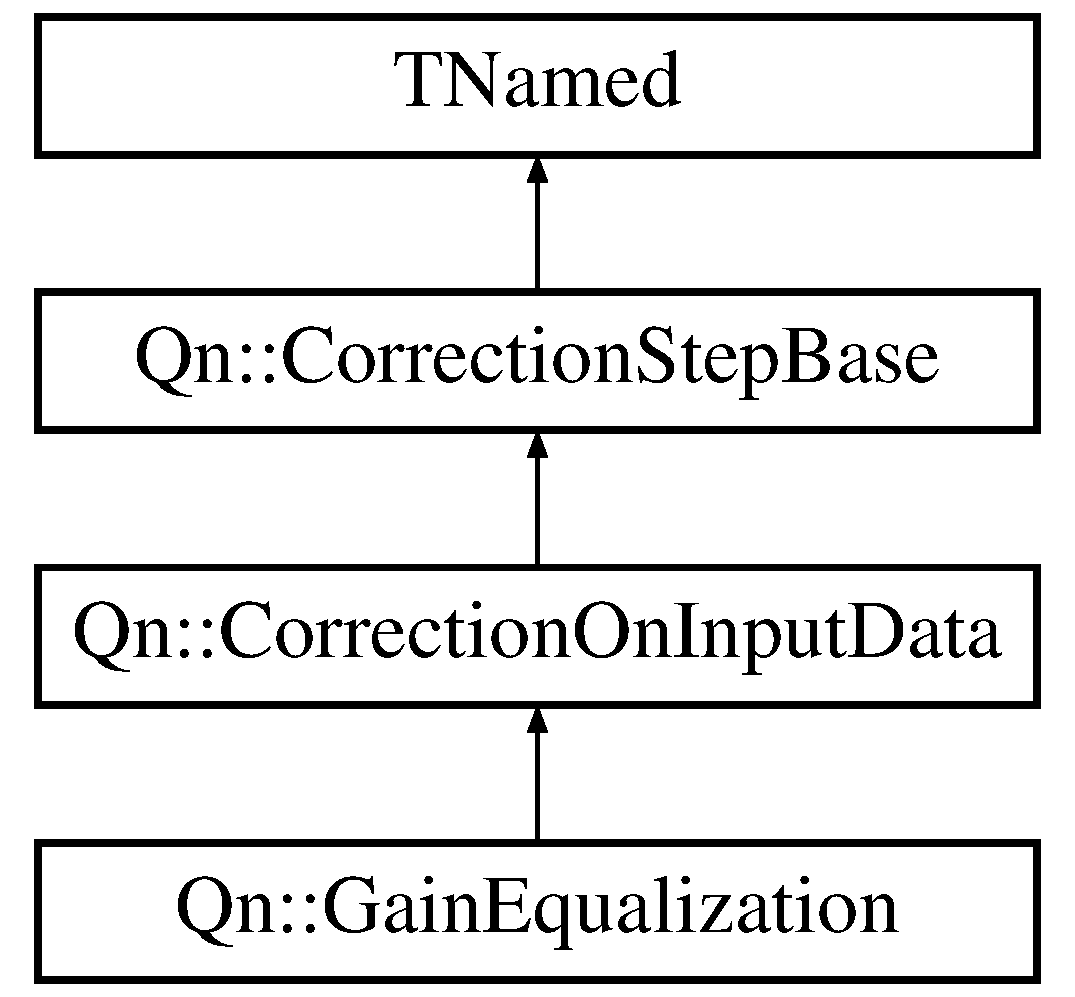
\includegraphics[height=4.000000cm]{classQn_1_1CorrectionOnInputData}
\end{center}
\end{figure}
\subsection*{Public Member Functions}
\begin{DoxyCompactItemize}
\item 
\mbox{\Hypertarget{classQn_1_1CorrectionOnInputData_a15e8ed1c6af8a630b16f3816306b2f1d}\label{classQn_1_1CorrectionOnInputData_a15e8ed1c6af8a630b16f3816306b2f1d}} 
\mbox{\hyperlink{classQn_1_1CorrectionOnInputData_a15e8ed1c6af8a630b16f3816306b2f1d}{Correction\+On\+Input\+Data}} ()
\begin{DoxyCompactList}\small\item\em Default constructor. \end{DoxyCompactList}\item 
\mbox{\hyperlink{classQn_1_1CorrectionOnInputData_a519a4d9222892b586efa89bb47cd46e8}{Correction\+On\+Input\+Data}} (const char $\ast$name, const char $\ast$key)
\item 
\mbox{\Hypertarget{classQn_1_1CorrectionOnInputData_a2cdd1d2536214897d3b61fc2463601c6}\label{classQn_1_1CorrectionOnInputData_a2cdd1d2536214897d3b61fc2463601c6}} 
virtual \mbox{\hyperlink{classQn_1_1CorrectionOnInputData_a2cdd1d2536214897d3b61fc2463601c6}{$\sim$\+Correction\+On\+Input\+Data}} ()
\begin{DoxyCompactList}\small\item\em Default destructor. \end{DoxyCompactList}\item 
virtual void \mbox{\hyperlink{classQn_1_1CorrectionOnInputData_adab1d79e0c216c6c981cd8d7ed271490}{Attached\+To\+Framework\+Manager}} ()=0
\item 
virtual Bool\+\_\+t \mbox{\hyperlink{classQn_1_1CorrectionOnInputData_a37c53966c0121ed0f7d764a9769690be}{Attach\+Input}} (T\+List $\ast$list)=0
\item 
virtual void \mbox{\hyperlink{classQn_1_1CorrectionOnInputData_ada5498cdbba9a7697a120f47fd64ae46}{After\+Inputs\+Attach\+Actions}} ()
\item 
virtual void \mbox{\hyperlink{classQn_1_1CorrectionOnInputData_a7da5cb5e6c82e28e2dd63d82ac82bc8a}{Create\+Support\+Data\+Structures}} ()=0
\item 
virtual Bool\+\_\+t \mbox{\hyperlink{classQn_1_1CorrectionOnInputData_a1556dd574545ef77d6b462020101bf39}{Create\+Support\+Histograms}} (T\+List $\ast$list)=0
\item 
virtual Bool\+\_\+t \mbox{\hyperlink{classQn_1_1CorrectionOnInputData_a42390a6c47f558faeb1e14d245dcbc4a}{Process\+Corrections}} (const double $\ast$variable\+Container)=0
\item 
virtual Bool\+\_\+t \mbox{\hyperlink{classQn_1_1CorrectionOnInputData_aff000eb0dbd571ac42eb0c4d3771ba69}{Process\+Data\+Collection}} (const double $\ast$variable\+Container)=0
\item 
virtual void \mbox{\hyperlink{classQn_1_1CorrectionOnInputData_a9072c5ffae945c464bed4ee3e60858a4}{Include\+Corrected\+Qn\+Vector}} (T\+List $\ast$list)
\item 
virtual void \mbox{\hyperlink{classQn_1_1CorrectionOnInputData_a8da92a3389c8654961199f123d5e6a6d}{Clear\+Correction\+Step}} ()=0
\item 
virtual Bool\+\_\+t \mbox{\hyperlink{classQn_1_1CorrectionOnInputData_a738e13f0a496811358ad3f5b86320ffa}{Is\+Being\+Applied}} () const
\item 
virtual Bool\+\_\+t \mbox{\hyperlink{classQn_1_1CorrectionOnInputData_a40b05b6db47e8dd52e1f6a616b9b9d3a}{Report\+Usage}} (T\+List $\ast$calibration\+List, T\+List $\ast$apply\+List)=0
\end{DoxyCompactItemize}
\subsection*{Friends}
\begin{DoxyCompactItemize}
\item 
\mbox{\Hypertarget{classQn_1_1CorrectionOnInputData_a0c85055b2faa6f776e4c3c0367a16417}\label{classQn_1_1CorrectionOnInputData_a0c85055b2faa6f776e4c3c0367a16417}} 
class {\bfseries Detector\+Configuration\+Channels}
\end{DoxyCompactItemize}
\subsection*{Additional Inherited Members}


\subsection{Constructor \& Destructor Documentation}
\mbox{\Hypertarget{classQn_1_1CorrectionOnInputData_a519a4d9222892b586efa89bb47cd46e8}\label{classQn_1_1CorrectionOnInputData_a519a4d9222892b586efa89bb47cd46e8}} 
\index{Qn\+::\+Correction\+On\+Input\+Data@{Qn\+::\+Correction\+On\+Input\+Data}!Correction\+On\+Input\+Data@{Correction\+On\+Input\+Data}}
\index{Correction\+On\+Input\+Data@{Correction\+On\+Input\+Data}!Qn\+::\+Correction\+On\+Input\+Data@{Qn\+::\+Correction\+On\+Input\+Data}}
\subsubsection{\texorpdfstring{Correction\+On\+Input\+Data()}{CorrectionOnInputData()}}
{\footnotesize\ttfamily Qn\+::\+Correction\+On\+Input\+Data\+::\+Correction\+On\+Input\+Data (\begin{DoxyParamCaption}\item[{const char $\ast$}]{name,  }\item[{const char $\ast$}]{key }\end{DoxyParamCaption})}

Normal constructor 
\begin{DoxyParams}{Parameters}
{\em name} & of the correction step \\
\hline
{\em key} & the associated ordering key \\
\hline
\end{DoxyParams}


\subsection{Member Function Documentation}
\mbox{\Hypertarget{classQn_1_1CorrectionOnInputData_ada5498cdbba9a7697a120f47fd64ae46}\label{classQn_1_1CorrectionOnInputData_ada5498cdbba9a7697a120f47fd64ae46}} 
\index{Qn\+::\+Correction\+On\+Input\+Data@{Qn\+::\+Correction\+On\+Input\+Data}!After\+Inputs\+Attach\+Actions@{After\+Inputs\+Attach\+Actions}}
\index{After\+Inputs\+Attach\+Actions@{After\+Inputs\+Attach\+Actions}!Qn\+::\+Correction\+On\+Input\+Data@{Qn\+::\+Correction\+On\+Input\+Data}}
\subsubsection{\texorpdfstring{After\+Inputs\+Attach\+Actions()}{AfterInputsAttachActions()}}
{\footnotesize\ttfamily virtual void Qn\+::\+Correction\+On\+Input\+Data\+::\+After\+Inputs\+Attach\+Actions (\begin{DoxyParamCaption}{ }\end{DoxyParamCaption})\hspace{0.3cm}{\ttfamily [inline]}, {\ttfamily [virtual]}}

Perform after calibration histograms attach actions It is used to inform the different correction step that all conditions for running the network are in place so it is time to check if their requirements are satisfied

Does nothing for the time being 

Implements \mbox{\hyperlink{classQn_1_1CorrectionStepBase_a0c32c1fceb1f1be225ef0407a806f9e2}{Qn\+::\+Correction\+Step\+Base}}.

\mbox{\Hypertarget{classQn_1_1CorrectionOnInputData_adab1d79e0c216c6c981cd8d7ed271490}\label{classQn_1_1CorrectionOnInputData_adab1d79e0c216c6c981cd8d7ed271490}} 
\index{Qn\+::\+Correction\+On\+Input\+Data@{Qn\+::\+Correction\+On\+Input\+Data}!Attached\+To\+Framework\+Manager@{Attached\+To\+Framework\+Manager}}
\index{Attached\+To\+Framework\+Manager@{Attached\+To\+Framework\+Manager}!Qn\+::\+Correction\+On\+Input\+Data@{Qn\+::\+Correction\+On\+Input\+Data}}
\subsubsection{\texorpdfstring{Attached\+To\+Framework\+Manager()}{AttachedToFrameworkManager()}}
{\footnotesize\ttfamily virtual void Qn\+::\+Correction\+On\+Input\+Data\+::\+Attached\+To\+Framework\+Manager (\begin{DoxyParamCaption}{ }\end{DoxyParamCaption})\hspace{0.3cm}{\ttfamily [pure virtual]}}

Informs when the detector configuration has been attached to the framework manager Basically this allows interaction between the different framework sections at configuration time Pure virtual function 

Implements \mbox{\hyperlink{classQn_1_1CorrectionStepBase_a0c255ad7095cd2aa89fcf1f1db068949}{Qn\+::\+Correction\+Step\+Base}}.



Implemented in \mbox{\hyperlink{classQn_1_1GainEqualization_a487cc533ff299196a16d0ee4688d1039}{Qn\+::\+Gain\+Equalization}}.

\mbox{\Hypertarget{classQn_1_1CorrectionOnInputData_a37c53966c0121ed0f7d764a9769690be}\label{classQn_1_1CorrectionOnInputData_a37c53966c0121ed0f7d764a9769690be}} 
\index{Qn\+::\+Correction\+On\+Input\+Data@{Qn\+::\+Correction\+On\+Input\+Data}!Attach\+Input@{Attach\+Input}}
\index{Attach\+Input@{Attach\+Input}!Qn\+::\+Correction\+On\+Input\+Data@{Qn\+::\+Correction\+On\+Input\+Data}}
\subsubsection{\texorpdfstring{Attach\+Input()}{AttachInput()}}
{\footnotesize\ttfamily virtual Bool\+\_\+t Qn\+::\+Correction\+On\+Input\+Data\+::\+Attach\+Input (\begin{DoxyParamCaption}\item[{T\+List $\ast$}]{list }\end{DoxyParamCaption})\hspace{0.3cm}{\ttfamily [pure virtual]}}

Attaches the needed input information to the correction step

Pure virtual function 
\begin{DoxyParams}{Parameters}
{\em list} & list where the inputs should be found \\
\hline
\end{DoxyParams}
\begin{DoxyReturn}{Returns}
k\+T\+R\+UE if everything went OK 
\end{DoxyReturn}


Implements \mbox{\hyperlink{classQn_1_1CorrectionStepBase_aa778d3926bb1ee463753466f2216187d}{Qn\+::\+Correction\+Step\+Base}}.



Implemented in \mbox{\hyperlink{classQn_1_1GainEqualization_a167a6348fcdf8c0f48cb16a3dd9d1c29}{Qn\+::\+Gain\+Equalization}}.

\mbox{\Hypertarget{classQn_1_1CorrectionOnInputData_a8da92a3389c8654961199f123d5e6a6d}\label{classQn_1_1CorrectionOnInputData_a8da92a3389c8654961199f123d5e6a6d}} 
\index{Qn\+::\+Correction\+On\+Input\+Data@{Qn\+::\+Correction\+On\+Input\+Data}!Clear\+Correction\+Step@{Clear\+Correction\+Step}}
\index{Clear\+Correction\+Step@{Clear\+Correction\+Step}!Qn\+::\+Correction\+On\+Input\+Data@{Qn\+::\+Correction\+On\+Input\+Data}}
\subsubsection{\texorpdfstring{Clear\+Correction\+Step()}{ClearCorrectionStep()}}
{\footnotesize\ttfamily virtual void Qn\+::\+Correction\+On\+Input\+Data\+::\+Clear\+Correction\+Step (\begin{DoxyParamCaption}{ }\end{DoxyParamCaption})\hspace{0.3cm}{\ttfamily [pure virtual]}}

Clean the correction to accept a new event Pure virtual function 

Implements \mbox{\hyperlink{classQn_1_1CorrectionStepBase_a879c47010a868c19bd08042445662e2e}{Qn\+::\+Correction\+Step\+Base}}.



Implemented in \mbox{\hyperlink{classQn_1_1GainEqualization_a8ee1f2ecf6929de35d455515a067ac9c}{Qn\+::\+Gain\+Equalization}}.

\mbox{\Hypertarget{classQn_1_1CorrectionOnInputData_a7da5cb5e6c82e28e2dd63d82ac82bc8a}\label{classQn_1_1CorrectionOnInputData_a7da5cb5e6c82e28e2dd63d82ac82bc8a}} 
\index{Qn\+::\+Correction\+On\+Input\+Data@{Qn\+::\+Correction\+On\+Input\+Data}!Create\+Support\+Data\+Structures@{Create\+Support\+Data\+Structures}}
\index{Create\+Support\+Data\+Structures@{Create\+Support\+Data\+Structures}!Qn\+::\+Correction\+On\+Input\+Data@{Qn\+::\+Correction\+On\+Input\+Data}}
\subsubsection{\texorpdfstring{Create\+Support\+Data\+Structures()}{CreateSupportDataStructures()}}
{\footnotesize\ttfamily virtual void Qn\+::\+Correction\+On\+Input\+Data\+::\+Create\+Support\+Data\+Structures (\begin{DoxyParamCaption}{ }\end{DoxyParamCaption})\hspace{0.3cm}{\ttfamily [pure virtual]}}

Asks for support data structures creation

Pure virtual function 

Implements \mbox{\hyperlink{classQn_1_1CorrectionStepBase_a800ac634950eb231d72033b03cc899cd}{Qn\+::\+Correction\+Step\+Base}}.



Implemented in \mbox{\hyperlink{classQn_1_1GainEqualization_a3b1da6e8711ef1e7dea394d3612ee8f9}{Qn\+::\+Gain\+Equalization}}.

\mbox{\Hypertarget{classQn_1_1CorrectionOnInputData_a1556dd574545ef77d6b462020101bf39}\label{classQn_1_1CorrectionOnInputData_a1556dd574545ef77d6b462020101bf39}} 
\index{Qn\+::\+Correction\+On\+Input\+Data@{Qn\+::\+Correction\+On\+Input\+Data}!Create\+Support\+Histograms@{Create\+Support\+Histograms}}
\index{Create\+Support\+Histograms@{Create\+Support\+Histograms}!Qn\+::\+Correction\+On\+Input\+Data@{Qn\+::\+Correction\+On\+Input\+Data}}
\subsubsection{\texorpdfstring{Create\+Support\+Histograms()}{CreateSupportHistograms()}}
{\footnotesize\ttfamily virtual Bool\+\_\+t Qn\+::\+Correction\+On\+Input\+Data\+::\+Create\+Support\+Histograms (\begin{DoxyParamCaption}\item[{T\+List $\ast$}]{list }\end{DoxyParamCaption})\hspace{0.3cm}{\ttfamily [pure virtual]}}

Asks for support histograms creation

Pure virtual function 
\begin{DoxyParams}{Parameters}
{\em list} & list where the histograms should be incorporated for its persistence \\
\hline
\end{DoxyParams}
\begin{DoxyReturn}{Returns}
k\+T\+R\+UE if everything went OK 
\end{DoxyReturn}


Implements \mbox{\hyperlink{classQn_1_1CorrectionStepBase_a156c05dc7a6a8e149674ccfb11e596c9}{Qn\+::\+Correction\+Step\+Base}}.



Implemented in \mbox{\hyperlink{classQn_1_1GainEqualization_a3f34cc42fe078c556d9acf98525490ce}{Qn\+::\+Gain\+Equalization}}.

\mbox{\Hypertarget{classQn_1_1CorrectionOnInputData_a9072c5ffae945c464bed4ee3e60858a4}\label{classQn_1_1CorrectionOnInputData_a9072c5ffae945c464bed4ee3e60858a4}} 
\index{Qn\+::\+Correction\+On\+Input\+Data@{Qn\+::\+Correction\+On\+Input\+Data}!Include\+Corrected\+Qn\+Vector@{Include\+Corrected\+Qn\+Vector}}
\index{Include\+Corrected\+Qn\+Vector@{Include\+Corrected\+Qn\+Vector}!Qn\+::\+Correction\+On\+Input\+Data@{Qn\+::\+Correction\+On\+Input\+Data}}
\subsubsection{\texorpdfstring{Include\+Corrected\+Qn\+Vector()}{IncludeCorrectedQnVector()}}
{\footnotesize\ttfamily virtual void Qn\+::\+Correction\+On\+Input\+Data\+::\+Include\+Corrected\+Qn\+Vector (\begin{DoxyParamCaption}\item[{T\+List $\ast$}]{list }\end{DoxyParamCaption})\hspace{0.3cm}{\ttfamily [inline]}, {\ttfamily [virtual]}}

Include the new corrected \mbox{\hyperlink{namespaceQn}{Qn}} vector into the passed list

Does nothing. Not applicable for corrections on input data 
\begin{DoxyParams}{Parameters}
{\em list} & list where the corrected \mbox{\hyperlink{namespaceQn}{Qn}} vector should be added \\
\hline
\end{DoxyParams}


Implements \mbox{\hyperlink{classQn_1_1CorrectionStepBase_a5f8936b56bfe4e5a7bf1e79775241500}{Qn\+::\+Correction\+Step\+Base}}.

\mbox{\Hypertarget{classQn_1_1CorrectionOnInputData_a738e13f0a496811358ad3f5b86320ffa}\label{classQn_1_1CorrectionOnInputData_a738e13f0a496811358ad3f5b86320ffa}} 
\index{Qn\+::\+Correction\+On\+Input\+Data@{Qn\+::\+Correction\+On\+Input\+Data}!Is\+Being\+Applied@{Is\+Being\+Applied}}
\index{Is\+Being\+Applied@{Is\+Being\+Applied}!Qn\+::\+Correction\+On\+Input\+Data@{Qn\+::\+Correction\+On\+Input\+Data}}
\subsubsection{\texorpdfstring{Is\+Being\+Applied()}{IsBeingApplied()}}
{\footnotesize\ttfamily virtual Bool\+\_\+t Qn\+::\+Correction\+On\+Input\+Data\+::\+Is\+Being\+Applied (\begin{DoxyParamCaption}{ }\end{DoxyParamCaption}) const\hspace{0.3cm}{\ttfamily [inline]}, {\ttfamily [virtual]}}

Reports if the correction step is being applied \begin{DoxyReturn}{Returns}
F\+A\+L\+SE, input data correction step dont make use of this service, yet 
\end{DoxyReturn}


Implements \mbox{\hyperlink{classQn_1_1CorrectionStepBase_aa99ab21886c2b4d8c3c6e1f60b84acc9}{Qn\+::\+Correction\+Step\+Base}}.

\mbox{\Hypertarget{classQn_1_1CorrectionOnInputData_a42390a6c47f558faeb1e14d245dcbc4a}\label{classQn_1_1CorrectionOnInputData_a42390a6c47f558faeb1e14d245dcbc4a}} 
\index{Qn\+::\+Correction\+On\+Input\+Data@{Qn\+::\+Correction\+On\+Input\+Data}!Process\+Corrections@{Process\+Corrections}}
\index{Process\+Corrections@{Process\+Corrections}!Qn\+::\+Correction\+On\+Input\+Data@{Qn\+::\+Correction\+On\+Input\+Data}}
\subsubsection{\texorpdfstring{Process\+Corrections()}{ProcessCorrections()}}
{\footnotesize\ttfamily virtual Bool\+\_\+t Qn\+::\+Correction\+On\+Input\+Data\+::\+Process\+Corrections (\begin{DoxyParamCaption}\item[{const double $\ast$}]{variable\+Container }\end{DoxyParamCaption})\hspace{0.3cm}{\ttfamily [pure virtual]}}

Processes the correction step

Pure virtual function \begin{DoxyReturn}{Returns}
k\+T\+R\+UE if everything went OK 
\end{DoxyReturn}


Implements \mbox{\hyperlink{classQn_1_1CorrectionStepBase_a773ff3bbe5e7c8bcfb11a4f4138af1e1}{Qn\+::\+Correction\+Step\+Base}}.



Implemented in \mbox{\hyperlink{classQn_1_1GainEqualization_ade22bc9b3aee596b6594d8a8d6fdc1f1}{Qn\+::\+Gain\+Equalization}}.

\mbox{\Hypertarget{classQn_1_1CorrectionOnInputData_aff000eb0dbd571ac42eb0c4d3771ba69}\label{classQn_1_1CorrectionOnInputData_aff000eb0dbd571ac42eb0c4d3771ba69}} 
\index{Qn\+::\+Correction\+On\+Input\+Data@{Qn\+::\+Correction\+On\+Input\+Data}!Process\+Data\+Collection@{Process\+Data\+Collection}}
\index{Process\+Data\+Collection@{Process\+Data\+Collection}!Qn\+::\+Correction\+On\+Input\+Data@{Qn\+::\+Correction\+On\+Input\+Data}}
\subsubsection{\texorpdfstring{Process\+Data\+Collection()}{ProcessDataCollection()}}
{\footnotesize\ttfamily virtual Bool\+\_\+t Qn\+::\+Correction\+On\+Input\+Data\+::\+Process\+Data\+Collection (\begin{DoxyParamCaption}\item[{const double $\ast$}]{variable\+Container }\end{DoxyParamCaption})\hspace{0.3cm}{\ttfamily [pure virtual]}}

Processes the correction step data collection

Pure virtual function \begin{DoxyReturn}{Returns}
k\+T\+R\+UE if everything went OK 
\end{DoxyReturn}


Implements \mbox{\hyperlink{classQn_1_1CorrectionStepBase_a77005ff85ae351cb290fee4adb41c029}{Qn\+::\+Correction\+Step\+Base}}.



Implemented in \mbox{\hyperlink{classQn_1_1GainEqualization_a9984ec9a1056bc3e336ff9ac50888641}{Qn\+::\+Gain\+Equalization}}.

\mbox{\Hypertarget{classQn_1_1CorrectionOnInputData_a40b05b6db47e8dd52e1f6a616b9b9d3a}\label{classQn_1_1CorrectionOnInputData_a40b05b6db47e8dd52e1f6a616b9b9d3a}} 
\index{Qn\+::\+Correction\+On\+Input\+Data@{Qn\+::\+Correction\+On\+Input\+Data}!Report\+Usage@{Report\+Usage}}
\index{Report\+Usage@{Report\+Usage}!Qn\+::\+Correction\+On\+Input\+Data@{Qn\+::\+Correction\+On\+Input\+Data}}
\subsubsection{\texorpdfstring{Report\+Usage()}{ReportUsage()}}
{\footnotesize\ttfamily virtual Bool\+\_\+t Qn\+::\+Correction\+On\+Input\+Data\+::\+Report\+Usage (\begin{DoxyParamCaption}\item[{T\+List $\ast$}]{calibration\+List,  }\item[{T\+List $\ast$}]{apply\+List }\end{DoxyParamCaption})\hspace{0.3cm}{\ttfamily [pure virtual]}}

Report on correction usage Pure virtual function Correction step should incorporate its name in calibration list if it is producing information calibration in the ongoing step and in the apply list if it is applying correction in the ongoing step. 
\begin{DoxyParams}{Parameters}
{\em calibration\+List} & list containing the correction steps producing calibration information \\
\hline
{\em apply\+List} & list containing the correction steps applying corrections \\
\hline
\end{DoxyParams}
\begin{DoxyReturn}{Returns}
k\+T\+R\+UE if the correction step is being applied 
\end{DoxyReturn}


Implements \mbox{\hyperlink{classQn_1_1CorrectionStepBase_a235ae6623fbbe26601b95f7e76753bfd}{Qn\+::\+Correction\+Step\+Base}}.



Implemented in \mbox{\hyperlink{classQn_1_1GainEqualization_af444038af10eb53d8bd6c8703d4e5629}{Qn\+::\+Gain\+Equalization}}.



The documentation for this class was generated from the following files\+:\begin{DoxyCompactItemize}
\item 
D\+T\+\_\+\+Flow/\+Qn\+Corrections/include/Correction\+On\+Input\+Data.\+h\item 
D\+T\+\_\+\+Flow/\+Qn\+Corrections/Correction\+On\+Input\+Data.\+cpp\end{DoxyCompactItemize}

\hypertarget{classQn_1_1CorrectionOnQvector}{}\section{Qn\+:\+:Correction\+On\+Qvector Class Reference}
\label{classQn_1_1CorrectionOnQvector}\index{Qn\+::\+Correction\+On\+Qvector@{Qn\+::\+Correction\+On\+Qvector}}
Inheritance diagram for Qn\+:\+:Correction\+On\+Qvector\+:\begin{figure}[H]
\begin{center}
\leavevmode
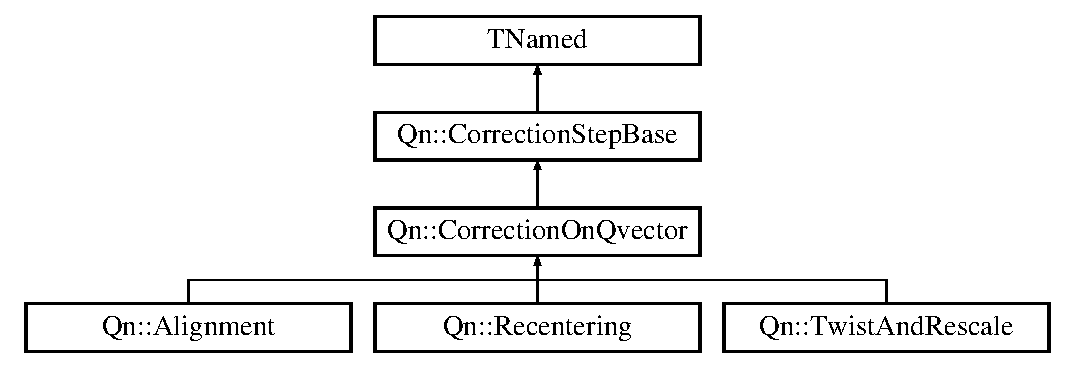
\includegraphics[height=4.000000cm]{classQn_1_1CorrectionOnQvector}
\end{center}
\end{figure}
\subsection*{Public Member Functions}
\begin{DoxyCompactItemize}
\item 
\mbox{\Hypertarget{classQn_1_1CorrectionOnQvector_a2f3658dab429c296773103d9d6fbd0c6}\label{classQn_1_1CorrectionOnQvector_a2f3658dab429c296773103d9d6fbd0c6}} 
\mbox{\hyperlink{classQn_1_1CorrectionOnQvector_a2f3658dab429c296773103d9d6fbd0c6}{Correction\+On\+Qvector}} ()
\begin{DoxyCompactList}\small\item\em Default constructor. \end{DoxyCompactList}\item 
\mbox{\hyperlink{classQn_1_1CorrectionOnQvector_af5c630667adbbd37bc6ca51445a8d37f}{Correction\+On\+Qvector}} (const char $\ast$name, const char $\ast$key)
\item 
\mbox{\Hypertarget{classQn_1_1CorrectionOnQvector_a2b0fdf26c68d941468873e4bcf311b30}\label{classQn_1_1CorrectionOnQvector_a2b0fdf26c68d941468873e4bcf311b30}} 
virtual \mbox{\hyperlink{classQn_1_1CorrectionOnQvector_a2b0fdf26c68d941468873e4bcf311b30}{$\sim$\+Correction\+On\+Qvector}} ()
\begin{DoxyCompactList}\small\item\em Default destructor. \end{DoxyCompactList}\item 
virtual void \mbox{\hyperlink{classQn_1_1CorrectionOnQvector_ad2d37eb35973c854c7ffa3560a97d510}{Attached\+To\+Framework\+Manager}} ()=0
\item 
virtual Bool\+\_\+t \mbox{\hyperlink{classQn_1_1CorrectionOnQvector_acb7165c2eb071517fa977484bee7e445}{Attach\+Input}} (T\+List $\ast$list)=0
\item 
virtual void \mbox{\hyperlink{classQn_1_1CorrectionOnQvector_afa95ec7804ade8097d92002e0ea05e44}{After\+Inputs\+Attach\+Actions}} ()=0
\item 
virtual void \mbox{\hyperlink{classQn_1_1CorrectionOnQvector_ac7c019bc36ac90618ed6e5fc768ca593}{Create\+Support\+Data\+Structures}} ()=0
\item 
virtual Bool\+\_\+t \mbox{\hyperlink{classQn_1_1CorrectionOnQvector_addcdd98787c99ea34a2511be2cdc8de4}{Create\+Support\+Histograms}} (T\+List $\ast$list)=0
\item 
virtual Bool\+\_\+t \mbox{\hyperlink{classQn_1_1CorrectionOnQvector_a2c2d7f0e48471fb9269f0b5f9aa3e836}{Process\+Corrections}} (const double $\ast$variable\+Container)=0
\item 
virtual Bool\+\_\+t \mbox{\hyperlink{classQn_1_1CorrectionOnQvector_a2c0a668d885b5a42503869303c859a0b}{Process\+Data\+Collection}} (const double $\ast$variable\+Container)=0
\item 
const \mbox{\hyperlink{classQn_1_1CorrectionQnVector}{Correction\+Qn\+Vector}} $\ast$ \mbox{\hyperlink{classQn_1_1CorrectionOnQvector_a3d6ef2f88326076972684d1d4115f5ab}{Get\+Corrected\+Qn\+Vector}} () const
\item 
virtual void \mbox{\hyperlink{classQn_1_1CorrectionOnQvector_a42d85f899f00a6e816969d5784c50765}{Include\+Corrected\+Qn\+Vector}} (T\+List $\ast$list)
\item 
virtual void \mbox{\hyperlink{classQn_1_1CorrectionOnQvector_aeba6db851f1a9ac5c6fd7adbd81de140}{Clear\+Correction\+Step}} ()=0
\item 
virtual Bool\+\_\+t \mbox{\hyperlink{classQn_1_1CorrectionOnQvector_a4d47a1c241b4bfd5ac98d6fdbc90eb79}{Is\+Being\+Applied}} () const =0
\item 
virtual Bool\+\_\+t \mbox{\hyperlink{classQn_1_1CorrectionOnQvector_a322860c299f0ca1db46ddd57c0828ba1}{Report\+Usage}} (T\+List $\ast$calibration\+List, T\+List $\ast$apply\+List)=0
\end{DoxyCompactItemize}
\subsection*{Protected Attributes}
\begin{DoxyCompactItemize}
\item 
\mbox{\Hypertarget{classQn_1_1CorrectionOnQvector_aa89ec5735e25de58957161ef4a909cfa}\label{classQn_1_1CorrectionOnQvector_aa89ec5735e25de58957161ef4a909cfa}} 
\mbox{\hyperlink{classQn_1_1CorrectionQnVector}{Correction\+Qn\+Vector}} $\ast$ \mbox{\hyperlink{classQn_1_1CorrectionOnQvector_aa89ec5735e25de58957161ef4a909cfa}{f\+Corrected\+Qn\+Vector}}
\begin{DoxyCompactList}\small\item\em ! the step corrected \mbox{\hyperlink{namespaceQn}{Qn}} vector \end{DoxyCompactList}\item 
const \mbox{\hyperlink{classQn_1_1CorrectionQnVector}{Correction\+Qn\+Vector}} $\ast$ \mbox{\hyperlink{classQn_1_1CorrectionOnQvector_a6579bcaa376e434aa5399f8cdbbd60dd}{f\+Input\+Qn\+Vector}}
\end{DoxyCompactItemize}
\subsection*{Additional Inherited Members}


\subsection{Constructor \& Destructor Documentation}
\mbox{\Hypertarget{classQn_1_1CorrectionOnQvector_af5c630667adbbd37bc6ca51445a8d37f}\label{classQn_1_1CorrectionOnQvector_af5c630667adbbd37bc6ca51445a8d37f}} 
\index{Qn\+::\+Correction\+On\+Qvector@{Qn\+::\+Correction\+On\+Qvector}!Correction\+On\+Qvector@{Correction\+On\+Qvector}}
\index{Correction\+On\+Qvector@{Correction\+On\+Qvector}!Qn\+::\+Correction\+On\+Qvector@{Qn\+::\+Correction\+On\+Qvector}}
\subsubsection{\texorpdfstring{Correction\+On\+Qvector()}{CorrectionOnQvector()}}
{\footnotesize\ttfamily Qn\+::\+Correction\+On\+Qvector\+::\+Correction\+On\+Qvector (\begin{DoxyParamCaption}\item[{const char $\ast$}]{name,  }\item[{const char $\ast$}]{key }\end{DoxyParamCaption})}

Normal constructor 
\begin{DoxyParams}{Parameters}
{\em name} & of the correction step \\
\hline
{\em key} & the associated ordering key \\
\hline
\end{DoxyParams}


\subsection{Member Function Documentation}
\mbox{\Hypertarget{classQn_1_1CorrectionOnQvector_afa95ec7804ade8097d92002e0ea05e44}\label{classQn_1_1CorrectionOnQvector_afa95ec7804ade8097d92002e0ea05e44}} 
\index{Qn\+::\+Correction\+On\+Qvector@{Qn\+::\+Correction\+On\+Qvector}!After\+Inputs\+Attach\+Actions@{After\+Inputs\+Attach\+Actions}}
\index{After\+Inputs\+Attach\+Actions@{After\+Inputs\+Attach\+Actions}!Qn\+::\+Correction\+On\+Qvector@{Qn\+::\+Correction\+On\+Qvector}}
\subsubsection{\texorpdfstring{After\+Inputs\+Attach\+Actions()}{AfterInputsAttachActions()}}
{\footnotesize\ttfamily virtual void Qn\+::\+Correction\+On\+Qvector\+::\+After\+Inputs\+Attach\+Actions (\begin{DoxyParamCaption}{ }\end{DoxyParamCaption})\hspace{0.3cm}{\ttfamily [pure virtual]}}

Perform after calibration histograms attach actions It is used to inform the different correction step that all conditions for running the network are in place so it is time to check if their requirements are satisfied

Pure virtual function 

Implements \mbox{\hyperlink{classQn_1_1CorrectionStepBase_a0c32c1fceb1f1be225ef0407a806f9e2}{Qn\+::\+Correction\+Step\+Base}}.



Implemented in \mbox{\hyperlink{classQn_1_1TwistAndRescale_ab9f2ec874c828bc88d70232ae4ca8e63}{Qn\+::\+Twist\+And\+Rescale}}, \mbox{\hyperlink{classQn_1_1Recentering_afce97632b1a2cc9ecf49a4f4768601dc}{Qn\+::\+Recentering}}, and \mbox{\hyperlink{classQn_1_1Alignment_a38007827bb028b2f2e0b4a3fb988d8ed}{Qn\+::\+Alignment}}.

\mbox{\Hypertarget{classQn_1_1CorrectionOnQvector_ad2d37eb35973c854c7ffa3560a97d510}\label{classQn_1_1CorrectionOnQvector_ad2d37eb35973c854c7ffa3560a97d510}} 
\index{Qn\+::\+Correction\+On\+Qvector@{Qn\+::\+Correction\+On\+Qvector}!Attached\+To\+Framework\+Manager@{Attached\+To\+Framework\+Manager}}
\index{Attached\+To\+Framework\+Manager@{Attached\+To\+Framework\+Manager}!Qn\+::\+Correction\+On\+Qvector@{Qn\+::\+Correction\+On\+Qvector}}
\subsubsection{\texorpdfstring{Attached\+To\+Framework\+Manager()}{AttachedToFrameworkManager()}}
{\footnotesize\ttfamily virtual void Qn\+::\+Correction\+On\+Qvector\+::\+Attached\+To\+Framework\+Manager (\begin{DoxyParamCaption}{ }\end{DoxyParamCaption})\hspace{0.3cm}{\ttfamily [pure virtual]}}

Informs when the detector configuration has been attached to the framework manager Basically this allows interaction between the different framework sections at configuration time Pure virtual function 

Implements \mbox{\hyperlink{classQn_1_1CorrectionStepBase_a0c255ad7095cd2aa89fcf1f1db068949}{Qn\+::\+Correction\+Step\+Base}}.



Implemented in \mbox{\hyperlink{classQn_1_1TwistAndRescale_a75b3e7001fabda74adcf1441ffab1435}{Qn\+::\+Twist\+And\+Rescale}}, \mbox{\hyperlink{classQn_1_1Recentering_aa51bf50f4a003ac79e7d8c669b1efdac}{Qn\+::\+Recentering}}, and \mbox{\hyperlink{classQn_1_1Alignment_ad9791cc06c9a7d8c407e1f783c7625f8}{Qn\+::\+Alignment}}.

\mbox{\Hypertarget{classQn_1_1CorrectionOnQvector_acb7165c2eb071517fa977484bee7e445}\label{classQn_1_1CorrectionOnQvector_acb7165c2eb071517fa977484bee7e445}} 
\index{Qn\+::\+Correction\+On\+Qvector@{Qn\+::\+Correction\+On\+Qvector}!Attach\+Input@{Attach\+Input}}
\index{Attach\+Input@{Attach\+Input}!Qn\+::\+Correction\+On\+Qvector@{Qn\+::\+Correction\+On\+Qvector}}
\subsubsection{\texorpdfstring{Attach\+Input()}{AttachInput()}}
{\footnotesize\ttfamily virtual Bool\+\_\+t Qn\+::\+Correction\+On\+Qvector\+::\+Attach\+Input (\begin{DoxyParamCaption}\item[{T\+List $\ast$}]{list }\end{DoxyParamCaption})\hspace{0.3cm}{\ttfamily [pure virtual]}}

Attaches the needed input information to the correction step

Pure virtual function 
\begin{DoxyParams}{Parameters}
{\em list} & list where the inputs should be found \\
\hline
\end{DoxyParams}
\begin{DoxyReturn}{Returns}
k\+T\+R\+UE if everything went OK 
\end{DoxyReturn}


Implements \mbox{\hyperlink{classQn_1_1CorrectionStepBase_aa778d3926bb1ee463753466f2216187d}{Qn\+::\+Correction\+Step\+Base}}.



Implemented in \mbox{\hyperlink{classQn_1_1TwistAndRescale_af6ca5526d392329f6f35adcc261de349}{Qn\+::\+Twist\+And\+Rescale}}, \mbox{\hyperlink{classQn_1_1Recentering_ae931dc184caefa05392992a15ae5b53f}{Qn\+::\+Recentering}}, and \mbox{\hyperlink{classQn_1_1Alignment_a3ae85e6706fe2a04098d339fcfff9113}{Qn\+::\+Alignment}}.

\mbox{\Hypertarget{classQn_1_1CorrectionOnQvector_aeba6db851f1a9ac5c6fd7adbd81de140}\label{classQn_1_1CorrectionOnQvector_aeba6db851f1a9ac5c6fd7adbd81de140}} 
\index{Qn\+::\+Correction\+On\+Qvector@{Qn\+::\+Correction\+On\+Qvector}!Clear\+Correction\+Step@{Clear\+Correction\+Step}}
\index{Clear\+Correction\+Step@{Clear\+Correction\+Step}!Qn\+::\+Correction\+On\+Qvector@{Qn\+::\+Correction\+On\+Qvector}}
\subsubsection{\texorpdfstring{Clear\+Correction\+Step()}{ClearCorrectionStep()}}
{\footnotesize\ttfamily virtual void Qn\+::\+Correction\+On\+Qvector\+::\+Clear\+Correction\+Step (\begin{DoxyParamCaption}{ }\end{DoxyParamCaption})\hspace{0.3cm}{\ttfamily [pure virtual]}}

Clean the correction to accept a new event Pure virtual function 

Implements \mbox{\hyperlink{classQn_1_1CorrectionStepBase_a879c47010a868c19bd08042445662e2e}{Qn\+::\+Correction\+Step\+Base}}.



Implemented in \mbox{\hyperlink{classQn_1_1TwistAndRescale_a07d06e5a437221d08bdba6078af1c596}{Qn\+::\+Twist\+And\+Rescale}}, \mbox{\hyperlink{classQn_1_1Recentering_a692ae2cc6740be54d0b1591a3db62d39}{Qn\+::\+Recentering}}, and \mbox{\hyperlink{classQn_1_1Alignment_aba2ba181fbf1572b646ed0d225cb773b}{Qn\+::\+Alignment}}.

\mbox{\Hypertarget{classQn_1_1CorrectionOnQvector_ac7c019bc36ac90618ed6e5fc768ca593}\label{classQn_1_1CorrectionOnQvector_ac7c019bc36ac90618ed6e5fc768ca593}} 
\index{Qn\+::\+Correction\+On\+Qvector@{Qn\+::\+Correction\+On\+Qvector}!Create\+Support\+Data\+Structures@{Create\+Support\+Data\+Structures}}
\index{Create\+Support\+Data\+Structures@{Create\+Support\+Data\+Structures}!Qn\+::\+Correction\+On\+Qvector@{Qn\+::\+Correction\+On\+Qvector}}
\subsubsection{\texorpdfstring{Create\+Support\+Data\+Structures()}{CreateSupportDataStructures()}}
{\footnotesize\ttfamily virtual void Qn\+::\+Correction\+On\+Qvector\+::\+Create\+Support\+Data\+Structures (\begin{DoxyParamCaption}{ }\end{DoxyParamCaption})\hspace{0.3cm}{\ttfamily [pure virtual]}}

Asks for support data structures creation

Pure virtual function 

Implements \mbox{\hyperlink{classQn_1_1CorrectionStepBase_a800ac634950eb231d72033b03cc899cd}{Qn\+::\+Correction\+Step\+Base}}.



Implemented in \mbox{\hyperlink{classQn_1_1TwistAndRescale_af28bb42098c1b3138769d1747f06468f}{Qn\+::\+Twist\+And\+Rescale}}, \mbox{\hyperlink{classQn_1_1Recentering_a6aa8507e24f482af1d7fdd55151b3d34}{Qn\+::\+Recentering}}, and \mbox{\hyperlink{classQn_1_1Alignment_afb0137bb2443eb44448bf15734096765}{Qn\+::\+Alignment}}.

\mbox{\Hypertarget{classQn_1_1CorrectionOnQvector_addcdd98787c99ea34a2511be2cdc8de4}\label{classQn_1_1CorrectionOnQvector_addcdd98787c99ea34a2511be2cdc8de4}} 
\index{Qn\+::\+Correction\+On\+Qvector@{Qn\+::\+Correction\+On\+Qvector}!Create\+Support\+Histograms@{Create\+Support\+Histograms}}
\index{Create\+Support\+Histograms@{Create\+Support\+Histograms}!Qn\+::\+Correction\+On\+Qvector@{Qn\+::\+Correction\+On\+Qvector}}
\subsubsection{\texorpdfstring{Create\+Support\+Histograms()}{CreateSupportHistograms()}}
{\footnotesize\ttfamily virtual Bool\+\_\+t Qn\+::\+Correction\+On\+Qvector\+::\+Create\+Support\+Histograms (\begin{DoxyParamCaption}\item[{T\+List $\ast$}]{list }\end{DoxyParamCaption})\hspace{0.3cm}{\ttfamily [pure virtual]}}

Asks for support histograms creation

Pure virtual function 
\begin{DoxyParams}{Parameters}
{\em list} & list where the histograms should be incorporated for its persistence \\
\hline
\end{DoxyParams}
\begin{DoxyReturn}{Returns}
k\+T\+R\+UE if everything went OK 
\end{DoxyReturn}


Implements \mbox{\hyperlink{classQn_1_1CorrectionStepBase_a156c05dc7a6a8e149674ccfb11e596c9}{Qn\+::\+Correction\+Step\+Base}}.



Implemented in \mbox{\hyperlink{classQn_1_1TwistAndRescale_a57826092f0c09750fe0f5919e2cdb617}{Qn\+::\+Twist\+And\+Rescale}}, \mbox{\hyperlink{classQn_1_1Recentering_accf0f1282e35bd0a94a2d93312ff6ad5}{Qn\+::\+Recentering}}, and \mbox{\hyperlink{classQn_1_1Alignment_ada53d00555fc8a59644b3db5a8584de3}{Qn\+::\+Alignment}}.

\mbox{\Hypertarget{classQn_1_1CorrectionOnQvector_a3d6ef2f88326076972684d1d4115f5ab}\label{classQn_1_1CorrectionOnQvector_a3d6ef2f88326076972684d1d4115f5ab}} 
\index{Qn\+::\+Correction\+On\+Qvector@{Qn\+::\+Correction\+On\+Qvector}!Get\+Corrected\+Qn\+Vector@{Get\+Corrected\+Qn\+Vector}}
\index{Get\+Corrected\+Qn\+Vector@{Get\+Corrected\+Qn\+Vector}!Qn\+::\+Correction\+On\+Qvector@{Qn\+::\+Correction\+On\+Qvector}}
\subsubsection{\texorpdfstring{Get\+Corrected\+Qn\+Vector()}{GetCorrectedQnVector()}}
{\footnotesize\ttfamily const \mbox{\hyperlink{classQn_1_1CorrectionQnVector}{Correction\+Qn\+Vector}}$\ast$ Qn\+::\+Correction\+On\+Qvector\+::\+Get\+Corrected\+Qn\+Vector (\begin{DoxyParamCaption}{ }\end{DoxyParamCaption}) const\hspace{0.3cm}{\ttfamily [inline]}}

Gets the corrected \mbox{\hyperlink{namespaceQn}{Qn}} vector \begin{DoxyReturn}{Returns}
the corrected \mbox{\hyperlink{namespaceQn}{Qn}} vector 
\end{DoxyReturn}
\mbox{\Hypertarget{classQn_1_1CorrectionOnQvector_a42d85f899f00a6e816969d5784c50765}\label{classQn_1_1CorrectionOnQvector_a42d85f899f00a6e816969d5784c50765}} 
\index{Qn\+::\+Correction\+On\+Qvector@{Qn\+::\+Correction\+On\+Qvector}!Include\+Corrected\+Qn\+Vector@{Include\+Corrected\+Qn\+Vector}}
\index{Include\+Corrected\+Qn\+Vector@{Include\+Corrected\+Qn\+Vector}!Qn\+::\+Correction\+On\+Qvector@{Qn\+::\+Correction\+On\+Qvector}}
\subsubsection{\texorpdfstring{Include\+Corrected\+Qn\+Vector()}{IncludeCorrectedQnVector()}}
{\footnotesize\ttfamily void Qn\+::\+Correction\+On\+Qvector\+::\+Include\+Corrected\+Qn\+Vector (\begin{DoxyParamCaption}\item[{T\+List $\ast$}]{list }\end{DoxyParamCaption})\hspace{0.3cm}{\ttfamily [virtual]}}

Include the new corrected \mbox{\hyperlink{namespaceQn}{Qn}} vector into the passed list

Adds the \mbox{\hyperlink{namespaceQn}{Qn}} vector to the passed list if the correction step is in correction states. 
\begin{DoxyParams}{Parameters}
{\em list} & list where the corrected \mbox{\hyperlink{namespaceQn}{Qn}} vector should be added \\
\hline
\end{DoxyParams}


Implements \mbox{\hyperlink{classQn_1_1CorrectionStepBase_a5f8936b56bfe4e5a7bf1e79775241500}{Qn\+::\+Correction\+Step\+Base}}.



Reimplemented in \mbox{\hyperlink{classQn_1_1TwistAndRescale_aad00583024f1a71458d6c86ba1cc4d44}{Qn\+::\+Twist\+And\+Rescale}}.

\mbox{\Hypertarget{classQn_1_1CorrectionOnQvector_a4d47a1c241b4bfd5ac98d6fdbc90eb79}\label{classQn_1_1CorrectionOnQvector_a4d47a1c241b4bfd5ac98d6fdbc90eb79}} 
\index{Qn\+::\+Correction\+On\+Qvector@{Qn\+::\+Correction\+On\+Qvector}!Is\+Being\+Applied@{Is\+Being\+Applied}}
\index{Is\+Being\+Applied@{Is\+Being\+Applied}!Qn\+::\+Correction\+On\+Qvector@{Qn\+::\+Correction\+On\+Qvector}}
\subsubsection{\texorpdfstring{Is\+Being\+Applied()}{IsBeingApplied()}}
{\footnotesize\ttfamily virtual Bool\+\_\+t Qn\+::\+Correction\+On\+Qvector\+::\+Is\+Being\+Applied (\begin{DoxyParamCaption}{ }\end{DoxyParamCaption}) const\hspace{0.3cm}{\ttfamily [pure virtual]}}

Reports if the correction step is being applied Pure virutal function \begin{DoxyReturn}{Returns}
T\+R\+UE if the correction step is being applied 
\end{DoxyReturn}


Implements \mbox{\hyperlink{classQn_1_1CorrectionStepBase_aa99ab21886c2b4d8c3c6e1f60b84acc9}{Qn\+::\+Correction\+Step\+Base}}.



Implemented in \mbox{\hyperlink{classQn_1_1TwistAndRescale_a82b3138efce50ea788122dd26ca964d7}{Qn\+::\+Twist\+And\+Rescale}}, \mbox{\hyperlink{classQn_1_1Recentering_a3849efa27b2827a2f307a100bc046916}{Qn\+::\+Recentering}}, and \mbox{\hyperlink{classQn_1_1Alignment_aaa38151d72ebf1aa97247ba07c4d16e5}{Qn\+::\+Alignment}}.

\mbox{\Hypertarget{classQn_1_1CorrectionOnQvector_a2c2d7f0e48471fb9269f0b5f9aa3e836}\label{classQn_1_1CorrectionOnQvector_a2c2d7f0e48471fb9269f0b5f9aa3e836}} 
\index{Qn\+::\+Correction\+On\+Qvector@{Qn\+::\+Correction\+On\+Qvector}!Process\+Corrections@{Process\+Corrections}}
\index{Process\+Corrections@{Process\+Corrections}!Qn\+::\+Correction\+On\+Qvector@{Qn\+::\+Correction\+On\+Qvector}}
\subsubsection{\texorpdfstring{Process\+Corrections()}{ProcessCorrections()}}
{\footnotesize\ttfamily virtual Bool\+\_\+t Qn\+::\+Correction\+On\+Qvector\+::\+Process\+Corrections (\begin{DoxyParamCaption}\item[{const double $\ast$}]{variable\+Container }\end{DoxyParamCaption})\hspace{0.3cm}{\ttfamily [pure virtual]}}

Processes the correction step

Pure virtual function \begin{DoxyReturn}{Returns}
k\+T\+R\+UE if everything went OK 
\end{DoxyReturn}


Implements \mbox{\hyperlink{classQn_1_1CorrectionStepBase_a773ff3bbe5e7c8bcfb11a4f4138af1e1}{Qn\+::\+Correction\+Step\+Base}}.



Implemented in \mbox{\hyperlink{classQn_1_1TwistAndRescale_a3bc16721deb0f73dbfcf0ae6cabe5b54}{Qn\+::\+Twist\+And\+Rescale}}, \mbox{\hyperlink{classQn_1_1Recentering_a78bd432f4eb1f13cf846176426dbe579}{Qn\+::\+Recentering}}, and \mbox{\hyperlink{classQn_1_1Alignment_a57b815d9ce4d0ae4f94ff6cb46eb2514}{Qn\+::\+Alignment}}.

\mbox{\Hypertarget{classQn_1_1CorrectionOnQvector_a2c0a668d885b5a42503869303c859a0b}\label{classQn_1_1CorrectionOnQvector_a2c0a668d885b5a42503869303c859a0b}} 
\index{Qn\+::\+Correction\+On\+Qvector@{Qn\+::\+Correction\+On\+Qvector}!Process\+Data\+Collection@{Process\+Data\+Collection}}
\index{Process\+Data\+Collection@{Process\+Data\+Collection}!Qn\+::\+Correction\+On\+Qvector@{Qn\+::\+Correction\+On\+Qvector}}
\subsubsection{\texorpdfstring{Process\+Data\+Collection()}{ProcessDataCollection()}}
{\footnotesize\ttfamily virtual Bool\+\_\+t Qn\+::\+Correction\+On\+Qvector\+::\+Process\+Data\+Collection (\begin{DoxyParamCaption}\item[{const double $\ast$}]{variable\+Container }\end{DoxyParamCaption})\hspace{0.3cm}{\ttfamily [pure virtual]}}

Processes the correction step data collection

Pure virtual function \begin{DoxyReturn}{Returns}
k\+T\+R\+UE if everything went OK 
\end{DoxyReturn}


Implements \mbox{\hyperlink{classQn_1_1CorrectionStepBase_a77005ff85ae351cb290fee4adb41c029}{Qn\+::\+Correction\+Step\+Base}}.



Implemented in \mbox{\hyperlink{classQn_1_1TwistAndRescale_ac0392e263ff658b876821ac06d5b2eff}{Qn\+::\+Twist\+And\+Rescale}}, \mbox{\hyperlink{classQn_1_1Recentering_a1e3efc8b261021b21732474eb7afa3ca}{Qn\+::\+Recentering}}, and \mbox{\hyperlink{classQn_1_1Alignment_af071fa4f51958ecfec6e6c58a7d84c84}{Qn\+::\+Alignment}}.

\mbox{\Hypertarget{classQn_1_1CorrectionOnQvector_a322860c299f0ca1db46ddd57c0828ba1}\label{classQn_1_1CorrectionOnQvector_a322860c299f0ca1db46ddd57c0828ba1}} 
\index{Qn\+::\+Correction\+On\+Qvector@{Qn\+::\+Correction\+On\+Qvector}!Report\+Usage@{Report\+Usage}}
\index{Report\+Usage@{Report\+Usage}!Qn\+::\+Correction\+On\+Qvector@{Qn\+::\+Correction\+On\+Qvector}}
\subsubsection{\texorpdfstring{Report\+Usage()}{ReportUsage()}}
{\footnotesize\ttfamily virtual Bool\+\_\+t Qn\+::\+Correction\+On\+Qvector\+::\+Report\+Usage (\begin{DoxyParamCaption}\item[{T\+List $\ast$}]{calibration\+List,  }\item[{T\+List $\ast$}]{apply\+List }\end{DoxyParamCaption})\hspace{0.3cm}{\ttfamily [pure virtual]}}

Report on correction usage Pure virtual function Correction step should incorporate its name in calibration list if it is producing information calibration in the ongoing step and in the apply list if it is applying correction in the ongoing step. 
\begin{DoxyParams}{Parameters}
{\em calibration\+List} & list containing the correction steps producing calibration information \\
\hline
{\em apply\+List} & list containing the correction steps applying corrections \\
\hline
\end{DoxyParams}
\begin{DoxyReturn}{Returns}
k\+T\+R\+UE if the correction step is being applied 
\end{DoxyReturn}


Implements \mbox{\hyperlink{classQn_1_1CorrectionStepBase_a235ae6623fbbe26601b95f7e76753bfd}{Qn\+::\+Correction\+Step\+Base}}.



Implemented in \mbox{\hyperlink{classQn_1_1TwistAndRescale_a2a6c985100656523b3d834a31d8f19a8}{Qn\+::\+Twist\+And\+Rescale}}, \mbox{\hyperlink{classQn_1_1Recentering_a06240f91a7656df95ac5aa55773b056a}{Qn\+::\+Recentering}}, and \mbox{\hyperlink{classQn_1_1Alignment_af8ef33833778e9af4bdb7b82f679c941}{Qn\+::\+Alignment}}.



\subsection{Member Data Documentation}
\mbox{\Hypertarget{classQn_1_1CorrectionOnQvector_a6579bcaa376e434aa5399f8cdbbd60dd}\label{classQn_1_1CorrectionOnQvector_a6579bcaa376e434aa5399f8cdbbd60dd}} 
\index{Qn\+::\+Correction\+On\+Qvector@{Qn\+::\+Correction\+On\+Qvector}!f\+Input\+Qn\+Vector@{f\+Input\+Qn\+Vector}}
\index{f\+Input\+Qn\+Vector@{f\+Input\+Qn\+Vector}!Qn\+::\+Correction\+On\+Qvector@{Qn\+::\+Correction\+On\+Qvector}}
\subsubsection{\texorpdfstring{f\+Input\+Qn\+Vector}{fInputQnVector}}
{\footnotesize\ttfamily const \mbox{\hyperlink{classQn_1_1CorrectionQnVector}{Correction\+Qn\+Vector}}$\ast$ Qn\+::\+Correction\+On\+Qvector\+::f\+Input\+Qn\+Vector\hspace{0.3cm}{\ttfamily [protected]}}

! the previous step corrected \mbox{\hyperlink{namespaceQn}{Qn}} vector 

The documentation for this class was generated from the following files\+:\begin{DoxyCompactItemize}
\item 
D\+T\+\_\+\+Flow/\+Qn\+Corrections/include/Correction\+On\+Qvector.\+h\item 
D\+T\+\_\+\+Flow/\+Qn\+Corrections/Correction\+On\+Qvector.\+cpp\end{DoxyCompactItemize}

\hypertarget{classQn_1_1CorrectionProfile}{}\section{Qn\+:\+:Correction\+Profile Class Reference}
\label{classQn_1_1CorrectionProfile}\index{Qn\+::\+Correction\+Profile@{Qn\+::\+Correction\+Profile}}
Inheritance diagram for Qn\+:\+:Correction\+Profile\+:\begin{figure}[H]
\begin{center}
\leavevmode
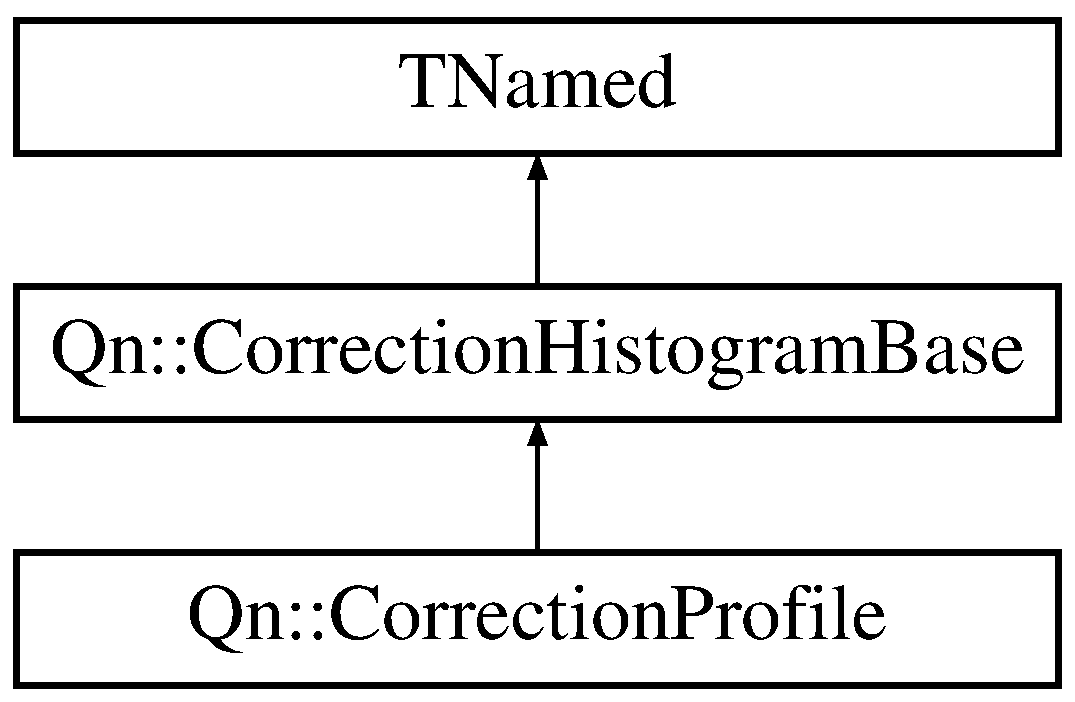
\includegraphics[height=3.000000cm]{classQn_1_1CorrectionProfile}
\end{center}
\end{figure}
\subsection*{Public Member Functions}
\begin{DoxyCompactItemize}
\item 
\mbox{\Hypertarget{classQn_1_1CorrectionProfile_af90a6f73d757a582036d0fed7133b811}\label{classQn_1_1CorrectionProfile_af90a6f73d757a582036d0fed7133b811}} 
\mbox{\hyperlink{classQn_1_1CorrectionProfile_af90a6f73d757a582036d0fed7133b811}{Correction\+Profile}} ()
\begin{DoxyCompactList}\small\item\em Default constructor. \end{DoxyCompactList}\item 
\mbox{\hyperlink{classQn_1_1CorrectionProfile_a509dc83514bf4e9a0aedcd37d98de4ed}{Correction\+Profile}} (const char $\ast$name, const char $\ast$title, \mbox{\hyperlink{classQn_1_1EventClassVariablesSet}{Event\+Class\+Variables\+Set}} \&ecvs, Option\+\_\+t $\ast$option=\char`\"{}\char`\"{})
\item 
virtual \mbox{\hyperlink{classQn_1_1CorrectionProfile_a571f318db482c796b420baedc637e185}{$\sim$\+Correction\+Profile}} ()
\item 
Bool\+\_\+t \mbox{\hyperlink{classQn_1_1CorrectionProfile_acdc3507cbdb49bef3fe821302635ca40}{Create\+Profile\+Histograms}} (T\+List $\ast$histogram\+List)
\item 
virtual Bool\+\_\+t \mbox{\hyperlink{classQn_1_1CorrectionProfile_a679319b8518152cf5563a87d77d87f2e}{Attach\+Histograms}} (T\+List $\ast$histogram\+List)
\item 
\mbox{\Hypertarget{classQn_1_1CorrectionProfile_a29060032cbf84f4f2891db40f466bf21}\label{classQn_1_1CorrectionProfile_a29060032cbf84f4f2891db40f466bf21}} 
virtual Bool\+\_\+t \mbox{\hyperlink{classQn_1_1CorrectionProfile_a29060032cbf84f4f2891db40f466bf21}{Attach\+Histograms}} (T\+List $\ast$histogram\+List, const Bool\+\_\+t $\ast$b\+Used\+Channel, const Int\+\_\+t $\ast$n\+Channel\+Group)
\begin{DoxyCompactList}\small\item\em wrong call for this class invoke base class behavior \end{DoxyCompactList}\item 
virtual Long64\+\_\+t \mbox{\hyperlink{classQn_1_1CorrectionProfile_a23eab8b418467aa8dc9ff6d590acd5c0}{Get\+Bin}} (const double $\ast$variable\+Container)
\item 
\mbox{\Hypertarget{classQn_1_1CorrectionProfile_ae670aae7149b53f64bf8461d1423f28d}\label{classQn_1_1CorrectionProfile_ae670aae7149b53f64bf8461d1423f28d}} 
virtual Long64\+\_\+t \mbox{\hyperlink{classQn_1_1CorrectionProfile_ae670aae7149b53f64bf8461d1423f28d}{Get\+Bin}} (const double $\ast$variable\+Container, Int\+\_\+t n\+Channel)
\begin{DoxyCompactList}\small\item\em wrong call for this class invoke base class behavior \end{DoxyCompactList}\item 
virtual Bool\+\_\+t \mbox{\hyperlink{classQn_1_1CorrectionProfile_a299a9d176bfeeb1966bedad226c7c4b2}{Bin\+Content\+Validated}} (Long64\+\_\+t bin)
\item 
virtual Float\+\_\+t \mbox{\hyperlink{classQn_1_1CorrectionProfile_ad6a10a5dd59ba94e9853699e63d902d4}{Get\+Bin\+Content}} (Long64\+\_\+t bin)
\item 
virtual Float\+\_\+t \mbox{\hyperlink{classQn_1_1CorrectionProfile_a2253439bc16a7611449b07fcfced1b53}{Get\+Bin\+Error}} (Long64\+\_\+t bin)
\item 
virtual void \mbox{\hyperlink{classQn_1_1CorrectionProfile_a93b95da0e85f546097075ac1958e84e6}{Fill}} (const double $\ast$variable\+Container, Float\+\_\+t weight)
\item 
\mbox{\Hypertarget{classQn_1_1CorrectionProfile_affeee38c64b7cf980278209d6f50dca1}\label{classQn_1_1CorrectionProfile_affeee38c64b7cf980278209d6f50dca1}} 
virtual void \mbox{\hyperlink{classQn_1_1CorrectionProfile_affeee38c64b7cf980278209d6f50dca1}{Fill}} (const double $\ast$variable\+Container, Int\+\_\+t n\+Channel, Float\+\_\+t weight)
\begin{DoxyCompactList}\small\item\em wrong call for this class invoke base class behavior \end{DoxyCompactList}\end{DoxyCompactItemize}
\subsection*{Additional Inherited Members}


\subsection{Constructor \& Destructor Documentation}
\mbox{\Hypertarget{classQn_1_1CorrectionProfile_a509dc83514bf4e9a0aedcd37d98de4ed}\label{classQn_1_1CorrectionProfile_a509dc83514bf4e9a0aedcd37d98de4ed}} 
\index{Qn\+::\+Correction\+Profile@{Qn\+::\+Correction\+Profile}!Correction\+Profile@{Correction\+Profile}}
\index{Correction\+Profile@{Correction\+Profile}!Qn\+::\+Correction\+Profile@{Qn\+::\+Correction\+Profile}}
\subsubsection{\texorpdfstring{Correction\+Profile()}{CorrectionProfile()}}
{\footnotesize\ttfamily Qn\+::\+Correction\+Profile\+::\+Correction\+Profile (\begin{DoxyParamCaption}\item[{const char $\ast$}]{name,  }\item[{const char $\ast$}]{title,  }\item[{\mbox{\hyperlink{classQn_1_1EventClassVariablesSet}{Event\+Class\+Variables\+Set}} \&}]{ecvs,  }\item[{Option\+\_\+t $\ast$}]{option = {\ttfamily \char`\"{}\char`\"{}} }\end{DoxyParamCaption})}

Normal constructor

Stores the set of variables that identify the different event classes passing them to its parent and prepares the object for actual histogram creation or attachment


\begin{DoxyParams}{Parameters}
{\em name} & base for the name of the histograms \\
\hline
{\em title} & base for the title of the histograms \\
\hline
{\em ecvs} & the event classes variables set \\
\hline
{\em option} & option for errors computation \textquotesingle{} \textquotesingle{} (Default) the bin errors are the standard error on the mean of the bin values\\
\hline
\end{DoxyParams}
\textquotesingle{}s\textquotesingle{} the bin are the standard deviation of of the bin values \mbox{\Hypertarget{classQn_1_1CorrectionProfile_a571f318db482c796b420baedc637e185}\label{classQn_1_1CorrectionProfile_a571f318db482c796b420baedc637e185}} 
\index{Qn\+::\+Correction\+Profile@{Qn\+::\+Correction\+Profile}!````~Correction\+Profile@{$\sim$\+Correction\+Profile}}
\index{````~Correction\+Profile@{$\sim$\+Correction\+Profile}!Qn\+::\+Correction\+Profile@{Qn\+::\+Correction\+Profile}}
\subsubsection{\texorpdfstring{$\sim$\+Correction\+Profile()}{~CorrectionProfile()}}
{\footnotesize\ttfamily Qn\+::\+Correction\+Profile\+::$\sim$\+Correction\+Profile (\begin{DoxyParamCaption}{ }\end{DoxyParamCaption})\hspace{0.3cm}{\ttfamily [virtual]}}

Default destructor

Does nothing because none of the members are own at destruction time 

\subsection{Member Function Documentation}
\mbox{\Hypertarget{classQn_1_1CorrectionProfile_a679319b8518152cf5563a87d77d87f2e}\label{classQn_1_1CorrectionProfile_a679319b8518152cf5563a87d77d87f2e}} 
\index{Qn\+::\+Correction\+Profile@{Qn\+::\+Correction\+Profile}!Attach\+Histograms@{Attach\+Histograms}}
\index{Attach\+Histograms@{Attach\+Histograms}!Qn\+::\+Correction\+Profile@{Qn\+::\+Correction\+Profile}}
\subsubsection{\texorpdfstring{Attach\+Histograms()}{AttachHistograms()}}
{\footnotesize\ttfamily Bool\+\_\+t Qn\+::\+Correction\+Profile\+::\+Attach\+Histograms (\begin{DoxyParamCaption}\item[{T\+List $\ast$}]{histogram\+List }\end{DoxyParamCaption})\hspace{0.3cm}{\ttfamily [virtual]}}

Attaches existing histograms as the support histograms for the profile function

The histograms are located in the passed list and if found and with the proper dimensions their references are stored in member variables.


\begin{DoxyParams}{Parameters}
{\em histogram\+List} & list where the histograms have to be located \\
\hline
\end{DoxyParams}
\begin{DoxyReturn}{Returns}
true if properly attached else false 
\end{DoxyReturn}


Reimplemented from \mbox{\hyperlink{classQn_1_1CorrectionHistogramBase_ad8bcd0079fe5db561780a522e46b7b16}{Qn\+::\+Correction\+Histogram\+Base}}.

\mbox{\Hypertarget{classQn_1_1CorrectionProfile_a299a9d176bfeeb1966bedad226c7c4b2}\label{classQn_1_1CorrectionProfile_a299a9d176bfeeb1966bedad226c7c4b2}} 
\index{Qn\+::\+Correction\+Profile@{Qn\+::\+Correction\+Profile}!Bin\+Content\+Validated@{Bin\+Content\+Validated}}
\index{Bin\+Content\+Validated@{Bin\+Content\+Validated}!Qn\+::\+Correction\+Profile@{Qn\+::\+Correction\+Profile}}
\subsubsection{\texorpdfstring{Bin\+Content\+Validated()}{BinContentValidated()}}
{\footnotesize\ttfamily Bool\+\_\+t Qn\+::\+Correction\+Profile\+::\+Bin\+Content\+Validated (\begin{DoxyParamCaption}\item[{Long64\+\_\+t}]{bin }\end{DoxyParamCaption})\hspace{0.3cm}{\ttfamily [virtual]}}

Check the validity of the content of the passed bin If the number of entries is lower than the minimum number of entries to validate it the bin content is not considered valid and k\+F\+A\+L\+SE is returned, otherwise k\+T\+R\+UE is returned 
\begin{DoxyParams}{Parameters}
{\em bin} & the bin to check its content validity \\
\hline
\end{DoxyParams}
\begin{DoxyReturn}{Returns}
k\+T\+R\+UE if the content is valid k\+F\+A\+L\+SE otherwise 
\end{DoxyReturn}


Implements \mbox{\hyperlink{classQn_1_1CorrectionHistogramBase_a4db2c92ceaffefaa91475a721612d80d}{Qn\+::\+Correction\+Histogram\+Base}}.

\mbox{\Hypertarget{classQn_1_1CorrectionProfile_acdc3507cbdb49bef3fe821302635ca40}\label{classQn_1_1CorrectionProfile_acdc3507cbdb49bef3fe821302635ca40}} 
\index{Qn\+::\+Correction\+Profile@{Qn\+::\+Correction\+Profile}!Create\+Profile\+Histograms@{Create\+Profile\+Histograms}}
\index{Create\+Profile\+Histograms@{Create\+Profile\+Histograms}!Qn\+::\+Correction\+Profile@{Qn\+::\+Correction\+Profile}}
\subsubsection{\texorpdfstring{Create\+Profile\+Histograms()}{CreateProfileHistograms()}}
{\footnotesize\ttfamily Bool\+\_\+t Qn\+::\+Correction\+Profile\+::\+Create\+Profile\+Histograms (\begin{DoxyParamCaption}\item[{T\+List $\ast$}]{histogram\+List }\end{DoxyParamCaption})}

Creates the support histograms for the profile function

Based in the event classes variables set in the parent class the values and entries multidimensional histograms are created.

Both histograms are added to the passed histogram list


\begin{DoxyParams}{Parameters}
{\em histogram\+List} & list where the histograms have to be added \\
\hline
\end{DoxyParams}
\begin{DoxyReturn}{Returns}
true if properly created 
\end{DoxyReturn}
\mbox{\Hypertarget{classQn_1_1CorrectionProfile_a93b95da0e85f546097075ac1958e84e6}\label{classQn_1_1CorrectionProfile_a93b95da0e85f546097075ac1958e84e6}} 
\index{Qn\+::\+Correction\+Profile@{Qn\+::\+Correction\+Profile}!Fill@{Fill}}
\index{Fill@{Fill}!Qn\+::\+Correction\+Profile@{Qn\+::\+Correction\+Profile}}
\subsubsection{\texorpdfstring{Fill()}{Fill()}}
{\footnotesize\ttfamily void Qn\+::\+Correction\+Profile\+::\+Fill (\begin{DoxyParamCaption}\item[{const double $\ast$}]{variable\+Container,  }\item[{Float\+\_\+t}]{weight }\end{DoxyParamCaption})\hspace{0.3cm}{\ttfamily [virtual]}}

Fills the histogram

The involved bin is computed according to the current variables content. The bin is then increased by the given weight and the entries also increased properly.


\begin{DoxyParams}{Parameters}
{\em variable\+Container} & the current variables conten addressed by var Id \\
\hline
{\em weight} & the increment in the bin content \\
\hline
\end{DoxyParams}


Reimplemented from \mbox{\hyperlink{classQn_1_1CorrectionHistogramBase_a16b7518942714780ec9ceb56bb517f0f}{Qn\+::\+Correction\+Histogram\+Base}}.

\mbox{\Hypertarget{classQn_1_1CorrectionProfile_a23eab8b418467aa8dc9ff6d590acd5c0}\label{classQn_1_1CorrectionProfile_a23eab8b418467aa8dc9ff6d590acd5c0}} 
\index{Qn\+::\+Correction\+Profile@{Qn\+::\+Correction\+Profile}!Get\+Bin@{Get\+Bin}}
\index{Get\+Bin@{Get\+Bin}!Qn\+::\+Correction\+Profile@{Qn\+::\+Correction\+Profile}}
\subsubsection{\texorpdfstring{Get\+Bin()}{GetBin()}}
{\footnotesize\ttfamily Long64\+\_\+t Qn\+::\+Correction\+Profile\+::\+Get\+Bin (\begin{DoxyParamCaption}\item[{const double $\ast$}]{variable\+Container }\end{DoxyParamCaption})\hspace{0.3cm}{\ttfamily [virtual]}}

Get the bin number for the current variable content

The bin number identifies the event class the current variable content points to.


\begin{DoxyParams}{Parameters}
{\em variable\+Container} & the current variables content addressed by var Id \\
\hline
\end{DoxyParams}
\begin{DoxyReturn}{Returns}
the associated bin to the current variables content 
\end{DoxyReturn}


Reimplemented from \mbox{\hyperlink{classQn_1_1CorrectionHistogramBase_ab1f64550f4e1812864da6f9f6ea565e6}{Qn\+::\+Correction\+Histogram\+Base}}.

\mbox{\Hypertarget{classQn_1_1CorrectionProfile_ad6a10a5dd59ba94e9853699e63d902d4}\label{classQn_1_1CorrectionProfile_ad6a10a5dd59ba94e9853699e63d902d4}} 
\index{Qn\+::\+Correction\+Profile@{Qn\+::\+Correction\+Profile}!Get\+Bin\+Content@{Get\+Bin\+Content}}
\index{Get\+Bin\+Content@{Get\+Bin\+Content}!Qn\+::\+Correction\+Profile@{Qn\+::\+Correction\+Profile}}
\subsubsection{\texorpdfstring{Get\+Bin\+Content()}{GetBinContent()}}
{\footnotesize\ttfamily Float\+\_\+t Qn\+::\+Correction\+Profile\+::\+Get\+Bin\+Content (\begin{DoxyParamCaption}\item[{Long64\+\_\+t}]{bin }\end{DoxyParamCaption})\hspace{0.3cm}{\ttfamily [virtual]}}

Get the bin content for the passed bin number

The bin number identifies a desired event class whose content is requested. If the bin content is not validated zero is returned.


\begin{DoxyParams}{Parameters}
{\em bin} & the interested bin number \\
\hline
\end{DoxyParams}
\begin{DoxyReturn}{Returns}
the bin number content 
\end{DoxyReturn}


Reimplemented from \mbox{\hyperlink{classQn_1_1CorrectionHistogramBase_a9e4e745a6f4cbebf5b9277d6d63bc9c7}{Qn\+::\+Correction\+Histogram\+Base}}.

\mbox{\Hypertarget{classQn_1_1CorrectionProfile_a2253439bc16a7611449b07fcfced1b53}\label{classQn_1_1CorrectionProfile_a2253439bc16a7611449b07fcfced1b53}} 
\index{Qn\+::\+Correction\+Profile@{Qn\+::\+Correction\+Profile}!Get\+Bin\+Error@{Get\+Bin\+Error}}
\index{Get\+Bin\+Error@{Get\+Bin\+Error}!Qn\+::\+Correction\+Profile@{Qn\+::\+Correction\+Profile}}
\subsubsection{\texorpdfstring{Get\+Bin\+Error()}{GetBinError()}}
{\footnotesize\ttfamily Float\+\_\+t Qn\+::\+Correction\+Profile\+::\+Get\+Bin\+Error (\begin{DoxyParamCaption}\item[{Long64\+\_\+t}]{bin }\end{DoxyParamCaption})\hspace{0.3cm}{\ttfamily [virtual]}}

Get the bin content error for the passed bin number

The bin number identifies a desired event class whose content error is requested. If the bin content is not validated zero is returned.


\begin{DoxyParams}{Parameters}
{\em bin} & the interested bin number \\
\hline
\end{DoxyParams}
\begin{DoxyReturn}{Returns}
the bin number content error 
\end{DoxyReturn}


Reimplemented from \mbox{\hyperlink{classQn_1_1CorrectionHistogramBase_a50a7dd4c5bbe5e4d0e405365c2a9104d}{Qn\+::\+Correction\+Histogram\+Base}}.



The documentation for this class was generated from the following files\+:\begin{DoxyCompactItemize}
\item 
D\+T\+\_\+\+Flow/\+Qn\+Corrections/include/Correction\+Profile.\+h\item 
D\+T\+\_\+\+Flow/\+Qn\+Corrections/Correction\+Profile.\+cpp\end{DoxyCompactItemize}

\hypertarget{classQn_1_1CorrectionProfile3DCorrelations}{}\section{Qn\+:\+:Correction\+Profile3\+D\+Correlations Class Reference}
\label{classQn_1_1CorrectionProfile3DCorrelations}\index{Qn\+::\+Correction\+Profile3\+D\+Correlations@{Qn\+::\+Correction\+Profile3\+D\+Correlations}}
Inheritance diagram for Qn\+:\+:Correction\+Profile3\+D\+Correlations\+:\begin{figure}[H]
\begin{center}
\leavevmode
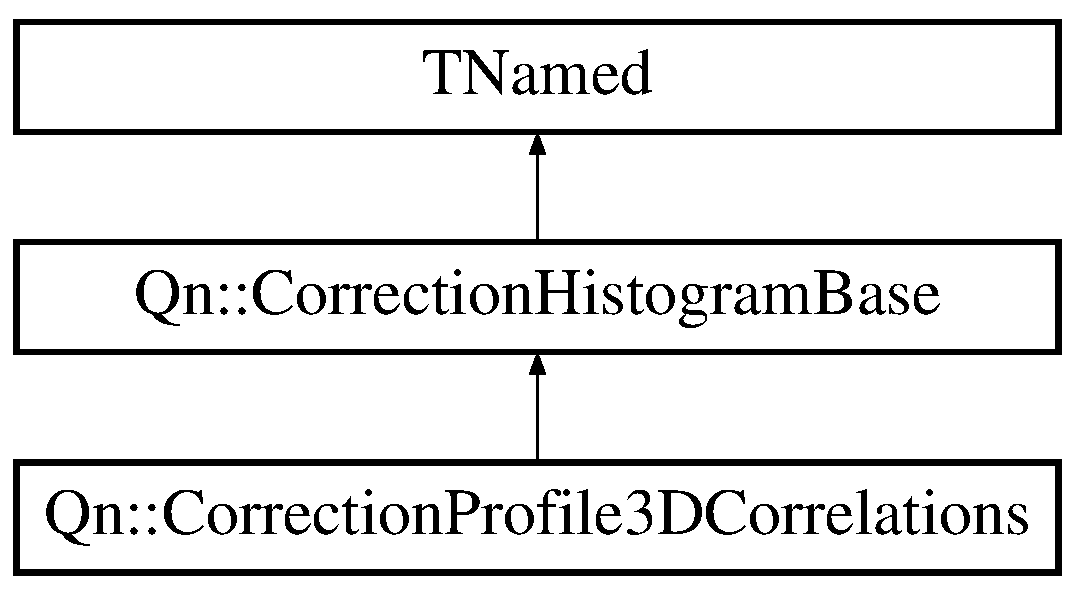
\includegraphics[height=3.000000cm]{classQn_1_1CorrectionProfile3DCorrelations}
\end{center}
\end{figure}
\subsection*{Public Member Functions}
\begin{DoxyCompactItemize}
\item 
\mbox{\Hypertarget{classQn_1_1CorrectionProfile3DCorrelations_a722a477bfa5bcd930256b71e8616414f}\label{classQn_1_1CorrectionProfile3DCorrelations_a722a477bfa5bcd930256b71e8616414f}} 
\mbox{\hyperlink{classQn_1_1CorrectionProfile3DCorrelations_a722a477bfa5bcd930256b71e8616414f}{Correction\+Profile3\+D\+Correlations}} ()
\begin{DoxyCompactList}\small\item\em Default constructor. \end{DoxyCompactList}\item 
\mbox{\hyperlink{classQn_1_1CorrectionProfile3DCorrelations_a7894d83ced5e0e9d7d4022984483c7d2}{Correction\+Profile3\+D\+Correlations}} (const char $\ast$name, const char $\ast$title, const char $\ast$nameA, const char $\ast$nameB, const char $\ast$nameC, \mbox{\hyperlink{classQn_1_1EventClassVariablesSet}{Event\+Class\+Variables\+Set}} \&ecvs, Option\+\_\+t $\ast$option=\char`\"{}\char`\"{})
\item 
virtual \mbox{\hyperlink{classQn_1_1CorrectionProfile3DCorrelations_a9f38225f6e469281047c83b2aaa9c495}{$\sim$\+Correction\+Profile3\+D\+Correlations}} ()
\item 
Bool\+\_\+t \mbox{\hyperlink{classQn_1_1CorrectionProfile3DCorrelations_aac1dd44c1c32c8e017c97cbac5cd911c}{Create\+Correlation\+Components\+Profile\+Histograms}} (T\+List $\ast$histogram\+List, Int\+\_\+t n\+No\+Of\+Harmonics, Int\+\_\+t n\+Harmonic\+Multiplier=1, Int\+\_\+t $\ast$harmonic\+Map=N\+U\+LL)
\item 
virtual Bool\+\_\+t \mbox{\hyperlink{classQn_1_1CorrectionProfile3DCorrelations_a6d6a1895f3362cd539f0249ad42d8b9c}{Attach\+Histograms}} (T\+List $\ast$histogram\+List)
\item 
\mbox{\Hypertarget{classQn_1_1CorrectionProfile3DCorrelations_a33bc769de702c401caa21b2d03cc705a}\label{classQn_1_1CorrectionProfile3DCorrelations_a33bc769de702c401caa21b2d03cc705a}} 
virtual Bool\+\_\+t \mbox{\hyperlink{classQn_1_1CorrectionProfile3DCorrelations_a33bc769de702c401caa21b2d03cc705a}{Attach\+Histograms}} (T\+List $\ast$histogram\+List, const Bool\+\_\+t $\ast$b\+Used\+Channel, const Int\+\_\+t $\ast$n\+Channel\+Group)
\begin{DoxyCompactList}\small\item\em wrong call for this class invoke base class behavior \end{DoxyCompactList}\item 
virtual Long64\+\_\+t \mbox{\hyperlink{classQn_1_1CorrectionProfile3DCorrelations_ad0e08d2b05447c1dbd10f2a8b55b840a}{Get\+Bin}} (const double $\ast$variable\+Container)
\item 
\mbox{\Hypertarget{classQn_1_1CorrectionProfile3DCorrelations_ae46e3ba4225d3640de7c2e5da8882c9f}\label{classQn_1_1CorrectionProfile3DCorrelations_ae46e3ba4225d3640de7c2e5da8882c9f}} 
virtual Long64\+\_\+t \mbox{\hyperlink{classQn_1_1CorrectionProfile3DCorrelations_ae46e3ba4225d3640de7c2e5da8882c9f}{Get\+Bin}} (const double $\ast$variable\+Container, Int\+\_\+t n\+Channel)
\begin{DoxyCompactList}\small\item\em wrong call for this class invoke base class behavior \end{DoxyCompactList}\item 
virtual Bool\+\_\+t \mbox{\hyperlink{classQn_1_1CorrectionProfile3DCorrelations_ad771201bd096e4e9bd028891baa032d9}{Bin\+Content\+Validated}} (Long64\+\_\+t bin)
\item 
virtual Float\+\_\+t \mbox{\hyperlink{classQn_1_1CorrectionProfile3DCorrelations_a1e51dc8db1fdfde5e6e5557bd87167e1}{Get\+X\+X\+Bin\+Content}} (const char $\ast$comb, Int\+\_\+t harmonic, Long64\+\_\+t bin)
\item 
virtual Float\+\_\+t \mbox{\hyperlink{classQn_1_1CorrectionProfile3DCorrelations_a8727b0b441c370f21a89ac507c049fdb}{Get\+X\+Y\+Bin\+Content}} (const char $\ast$comb, Int\+\_\+t harmonic, Long64\+\_\+t bin)
\item 
virtual Float\+\_\+t \mbox{\hyperlink{classQn_1_1CorrectionProfile3DCorrelations_a1ac93d3f7efb198491199728065e687b}{Get\+Y\+X\+Bin\+Content}} (const char $\ast$comb, Int\+\_\+t harmonic, Long64\+\_\+t bin)
\item 
virtual Float\+\_\+t \mbox{\hyperlink{classQn_1_1CorrectionProfile3DCorrelations_a7a58783cf79eeacf32370fc424a587a4}{Get\+Y\+Y\+Bin\+Content}} (const char $\ast$comb, Int\+\_\+t harmonic, Long64\+\_\+t bin)
\item 
virtual Float\+\_\+t \mbox{\hyperlink{classQn_1_1CorrectionProfile3DCorrelations_abbb27758a2f9b4c82d057e405e27fdd5}{Get\+X\+X\+Bin\+Error}} (const char $\ast$comb, Int\+\_\+t harmonic, Long64\+\_\+t bin)
\item 
virtual Float\+\_\+t \mbox{\hyperlink{classQn_1_1CorrectionProfile3DCorrelations_aeb58a03c96909827494763fd4dd44e30}{Get\+X\+Y\+Bin\+Error}} (const char $\ast$comb, Int\+\_\+t harmonic, Long64\+\_\+t bin)
\item 
virtual Float\+\_\+t \mbox{\hyperlink{classQn_1_1CorrectionProfile3DCorrelations_ac26f18268f0f9c6398ec5491133219dd}{Get\+Y\+X\+Bin\+Error}} (const char $\ast$comb, Int\+\_\+t harmonic, Long64\+\_\+t bin)
\item 
virtual Float\+\_\+t \mbox{\hyperlink{classQn_1_1CorrectionProfile3DCorrelations_ad1727f73c8583d6efceaefb92f7698fa}{Get\+Y\+Y\+Bin\+Error}} (const char $\ast$comb, Int\+\_\+t harmonic, Long64\+\_\+t bin)
\item 
void \mbox{\hyperlink{classQn_1_1CorrectionProfile3DCorrelations_a0e3a3f2897838bfc0480ced2d0883e4e}{Fill}} (const \mbox{\hyperlink{classQn_1_1CorrectionQnVector}{Correction\+Qn\+Vector}} $\ast$QnA, const \mbox{\hyperlink{classQn_1_1CorrectionQnVector}{Correction\+Qn\+Vector}} $\ast$QnB, const \mbox{\hyperlink{classQn_1_1CorrectionQnVector}{Correction\+Qn\+Vector}} $\ast$QnC, const double $\ast$variable\+Container)
\item 
\mbox{\Hypertarget{classQn_1_1CorrectionProfile3DCorrelations_a2c06b157700f9e1c8a11d15df6b4b816}\label{classQn_1_1CorrectionProfile3DCorrelations_a2c06b157700f9e1c8a11d15df6b4b816}} 
virtual Float\+\_\+t \mbox{\hyperlink{classQn_1_1CorrectionProfile3DCorrelations_a2c06b157700f9e1c8a11d15df6b4b816}{Get\+X\+X\+Bin\+Content}} (Long64\+\_\+t bin)
\begin{DoxyCompactList}\small\item\em wrong call for this class invoke base class behavior \end{DoxyCompactList}\item 
\mbox{\Hypertarget{classQn_1_1CorrectionProfile3DCorrelations_a47c118a0603a6ca87c505f940e35249c}\label{classQn_1_1CorrectionProfile3DCorrelations_a47c118a0603a6ca87c505f940e35249c}} 
virtual Float\+\_\+t \mbox{\hyperlink{classQn_1_1CorrectionProfile3DCorrelations_a47c118a0603a6ca87c505f940e35249c}{Get\+X\+Y\+Bin\+Content}} (Long64\+\_\+t bin)
\begin{DoxyCompactList}\small\item\em wrong call for this class invoke base class behavior \end{DoxyCompactList}\item 
\mbox{\Hypertarget{classQn_1_1CorrectionProfile3DCorrelations_a779657f7aabd240f26fae0690a5b24a7}\label{classQn_1_1CorrectionProfile3DCorrelations_a779657f7aabd240f26fae0690a5b24a7}} 
virtual Float\+\_\+t \mbox{\hyperlink{classQn_1_1CorrectionProfile3DCorrelations_a779657f7aabd240f26fae0690a5b24a7}{Get\+Y\+X\+Bin\+Content}} (Long64\+\_\+t bin)
\begin{DoxyCompactList}\small\item\em wrong call for this class invoke base class behavior \end{DoxyCompactList}\item 
\mbox{\Hypertarget{classQn_1_1CorrectionProfile3DCorrelations_ab911ed8b66eca8bcc200ed1abf843e7b}\label{classQn_1_1CorrectionProfile3DCorrelations_ab911ed8b66eca8bcc200ed1abf843e7b}} 
virtual Float\+\_\+t \mbox{\hyperlink{classQn_1_1CorrectionProfile3DCorrelations_ab911ed8b66eca8bcc200ed1abf843e7b}{Get\+Y\+Y\+Bin\+Content}} (Long64\+\_\+t bin)
\begin{DoxyCompactList}\small\item\em wrong call for this class invoke base class behavior \end{DoxyCompactList}\item 
\mbox{\Hypertarget{classQn_1_1CorrectionProfile3DCorrelations_a707cfe8bdc3ff7499a007f3d09688423}\label{classQn_1_1CorrectionProfile3DCorrelations_a707cfe8bdc3ff7499a007f3d09688423}} 
virtual Float\+\_\+t \mbox{\hyperlink{classQn_1_1CorrectionProfile3DCorrelations_a707cfe8bdc3ff7499a007f3d09688423}{Get\+X\+X\+Bin\+Error}} (Long64\+\_\+t bin)
\begin{DoxyCompactList}\small\item\em wrong call for this class invoke base class behavior \end{DoxyCompactList}\item 
\mbox{\Hypertarget{classQn_1_1CorrectionProfile3DCorrelations_a4fe7d57e81c21e72da9c0ca3c3d9f238}\label{classQn_1_1CorrectionProfile3DCorrelations_a4fe7d57e81c21e72da9c0ca3c3d9f238}} 
virtual Float\+\_\+t \mbox{\hyperlink{classQn_1_1CorrectionProfile3DCorrelations_a4fe7d57e81c21e72da9c0ca3c3d9f238}{Get\+X\+Y\+Bin\+Error}} (Long64\+\_\+t bin)
\begin{DoxyCompactList}\small\item\em wrong call for this class invoke base class behavior \end{DoxyCompactList}\item 
\mbox{\Hypertarget{classQn_1_1CorrectionProfile3DCorrelations_a40f70d3632b88451fb7f4bea2cd40650}\label{classQn_1_1CorrectionProfile3DCorrelations_a40f70d3632b88451fb7f4bea2cd40650}} 
virtual Float\+\_\+t \mbox{\hyperlink{classQn_1_1CorrectionProfile3DCorrelations_a40f70d3632b88451fb7f4bea2cd40650}{Get\+Y\+X\+Bin\+Error}} (Long64\+\_\+t bin)
\begin{DoxyCompactList}\small\item\em wrong call for this class invoke base class behavior \end{DoxyCompactList}\item 
\mbox{\Hypertarget{classQn_1_1CorrectionProfile3DCorrelations_a02c551ac645a7b5a3f2413a7ccb8985a}\label{classQn_1_1CorrectionProfile3DCorrelations_a02c551ac645a7b5a3f2413a7ccb8985a}} 
virtual Float\+\_\+t \mbox{\hyperlink{classQn_1_1CorrectionProfile3DCorrelations_a02c551ac645a7b5a3f2413a7ccb8985a}{Get\+Y\+Y\+Bin\+Error}} (Long64\+\_\+t bin)
\begin{DoxyCompactList}\small\item\em wrong call for this class invoke base class behavior \end{DoxyCompactList}\item 
\mbox{\Hypertarget{classQn_1_1CorrectionProfile3DCorrelations_a36e3cae66cf3f957b5e92a78b45aea6a}\label{classQn_1_1CorrectionProfile3DCorrelations_a36e3cae66cf3f957b5e92a78b45aea6a}} 
virtual Float\+\_\+t \mbox{\hyperlink{classQn_1_1CorrectionProfile3DCorrelations_a36e3cae66cf3f957b5e92a78b45aea6a}{Get\+X\+X\+Bin\+Content}} (Int\+\_\+t harmonic, Long64\+\_\+t bin)
\begin{DoxyCompactList}\small\item\em wrong call for this class invoke base class behavior \end{DoxyCompactList}\item 
\mbox{\Hypertarget{classQn_1_1CorrectionProfile3DCorrelations_a4471deccdf29c330cdbbbbb47d949d08}\label{classQn_1_1CorrectionProfile3DCorrelations_a4471deccdf29c330cdbbbbb47d949d08}} 
virtual Float\+\_\+t \mbox{\hyperlink{classQn_1_1CorrectionProfile3DCorrelations_a4471deccdf29c330cdbbbbb47d949d08}{Get\+X\+Y\+Bin\+Content}} (Int\+\_\+t harmonic, Long64\+\_\+t bin)
\begin{DoxyCompactList}\small\item\em wrong call for this class invoke base class behavior \end{DoxyCompactList}\item 
\mbox{\Hypertarget{classQn_1_1CorrectionProfile3DCorrelations_a27127ed9f52b6b4b7ec2df59f88c457f}\label{classQn_1_1CorrectionProfile3DCorrelations_a27127ed9f52b6b4b7ec2df59f88c457f}} 
virtual Float\+\_\+t \mbox{\hyperlink{classQn_1_1CorrectionProfile3DCorrelations_a27127ed9f52b6b4b7ec2df59f88c457f}{Get\+Y\+X\+Bin\+Content}} (Int\+\_\+t harmonic, Long64\+\_\+t bin)
\begin{DoxyCompactList}\small\item\em wrong call for this class invoke base class behavior \end{DoxyCompactList}\item 
\mbox{\Hypertarget{classQn_1_1CorrectionProfile3DCorrelations_a64bac99b0b417241e68ba9d133d07ef4}\label{classQn_1_1CorrectionProfile3DCorrelations_a64bac99b0b417241e68ba9d133d07ef4}} 
virtual Float\+\_\+t \mbox{\hyperlink{classQn_1_1CorrectionProfile3DCorrelations_a64bac99b0b417241e68ba9d133d07ef4}{Get\+Y\+Y\+Bin\+Content}} (Int\+\_\+t harmonic, Long64\+\_\+t bin)
\begin{DoxyCompactList}\small\item\em wrong call for this class invoke base class behavior \end{DoxyCompactList}\item 
\mbox{\Hypertarget{classQn_1_1CorrectionProfile3DCorrelations_a5b8a043e3d3377b4201c87085e12dd5b}\label{classQn_1_1CorrectionProfile3DCorrelations_a5b8a043e3d3377b4201c87085e12dd5b}} 
virtual Float\+\_\+t \mbox{\hyperlink{classQn_1_1CorrectionProfile3DCorrelations_a5b8a043e3d3377b4201c87085e12dd5b}{Get\+X\+X\+Bin\+Error}} (Int\+\_\+t harmonic, Long64\+\_\+t bin)
\begin{DoxyCompactList}\small\item\em wrong call for this class invoke base class behavior \end{DoxyCompactList}\item 
\mbox{\Hypertarget{classQn_1_1CorrectionProfile3DCorrelations_a44be0e49b21d3e4528d65e0c7398ddd0}\label{classQn_1_1CorrectionProfile3DCorrelations_a44be0e49b21d3e4528d65e0c7398ddd0}} 
virtual Float\+\_\+t \mbox{\hyperlink{classQn_1_1CorrectionProfile3DCorrelations_a44be0e49b21d3e4528d65e0c7398ddd0}{Get\+X\+Y\+Bin\+Error}} (Int\+\_\+t harmonic, Long64\+\_\+t bin)
\begin{DoxyCompactList}\small\item\em wrong call for this class invoke base class behavior \end{DoxyCompactList}\item 
\mbox{\Hypertarget{classQn_1_1CorrectionProfile3DCorrelations_a3f6a74c4e11f5cf25e9e790f8bda20ba}\label{classQn_1_1CorrectionProfile3DCorrelations_a3f6a74c4e11f5cf25e9e790f8bda20ba}} 
virtual Float\+\_\+t \mbox{\hyperlink{classQn_1_1CorrectionProfile3DCorrelations_a3f6a74c4e11f5cf25e9e790f8bda20ba}{Get\+Y\+X\+Bin\+Error}} (Int\+\_\+t harmonic, Long64\+\_\+t bin)
\begin{DoxyCompactList}\small\item\em wrong call for this class invoke base class behavior \end{DoxyCompactList}\item 
\mbox{\Hypertarget{classQn_1_1CorrectionProfile3DCorrelations_a114a4f0454ad223929c3a16504c408aa}\label{classQn_1_1CorrectionProfile3DCorrelations_a114a4f0454ad223929c3a16504c408aa}} 
virtual Float\+\_\+t \mbox{\hyperlink{classQn_1_1CorrectionProfile3DCorrelations_a114a4f0454ad223929c3a16504c408aa}{Get\+Y\+Y\+Bin\+Error}} (Int\+\_\+t harmonic, Long64\+\_\+t bin)
\begin{DoxyCompactList}\small\item\em wrong call for this class invoke base class behavior \end{DoxyCompactList}\item 
\mbox{\Hypertarget{classQn_1_1CorrectionProfile3DCorrelations_abd5a109f482219cb8f8a48ec3fbf4f6d}\label{classQn_1_1CorrectionProfile3DCorrelations_abd5a109f482219cb8f8a48ec3fbf4f6d}} 
virtual void \mbox{\hyperlink{classQn_1_1CorrectionProfile3DCorrelations_abd5a109f482219cb8f8a48ec3fbf4f6d}{Fill}} (const double $\ast$variable\+Container, Float\+\_\+t weight)
\begin{DoxyCompactList}\small\item\em wrong call for this class invoke base class behavior \end{DoxyCompactList}\item 
\mbox{\Hypertarget{classQn_1_1CorrectionProfile3DCorrelations_a1fb7c64ce84f414394b66cb21b2775c0}\label{classQn_1_1CorrectionProfile3DCorrelations_a1fb7c64ce84f414394b66cb21b2775c0}} 
virtual void \mbox{\hyperlink{classQn_1_1CorrectionProfile3DCorrelations_a1fb7c64ce84f414394b66cb21b2775c0}{Fill}} (const double $\ast$variable\+Container, Int\+\_\+t n\+Channel, Float\+\_\+t weight)
\begin{DoxyCompactList}\small\item\em wrong call for this class invoke base class behavior \end{DoxyCompactList}\end{DoxyCompactItemize}
\subsection*{Additional Inherited Members}


\subsection{Constructor \& Destructor Documentation}
\mbox{\Hypertarget{classQn_1_1CorrectionProfile3DCorrelations_a7894d83ced5e0e9d7d4022984483c7d2}\label{classQn_1_1CorrectionProfile3DCorrelations_a7894d83ced5e0e9d7d4022984483c7d2}} 
\index{Qn\+::\+Correction\+Profile3\+D\+Correlations@{Qn\+::\+Correction\+Profile3\+D\+Correlations}!Correction\+Profile3\+D\+Correlations@{Correction\+Profile3\+D\+Correlations}}
\index{Correction\+Profile3\+D\+Correlations@{Correction\+Profile3\+D\+Correlations}!Qn\+::\+Correction\+Profile3\+D\+Correlations@{Qn\+::\+Correction\+Profile3\+D\+Correlations}}
\subsubsection{\texorpdfstring{Correction\+Profile3\+D\+Correlations()}{CorrectionProfile3DCorrelations()}}
{\footnotesize\ttfamily Qn\+::\+Correction\+Profile3\+D\+Correlations\+::\+Correction\+Profile3\+D\+Correlations (\begin{DoxyParamCaption}\item[{const char $\ast$}]{name,  }\item[{const char $\ast$}]{title,  }\item[{const char $\ast$}]{nameA,  }\item[{const char $\ast$}]{nameB,  }\item[{const char $\ast$}]{nameC,  }\item[{\mbox{\hyperlink{classQn_1_1EventClassVariablesSet}{Event\+Class\+Variables\+Set}} \&}]{ecvs,  }\item[{Option\+\_\+t $\ast$}]{option = {\ttfamily \char`\"{}\char`\"{}} }\end{DoxyParamCaption})}

Normal constructor

Stores the set of variables that identify the different event classes passing them to its parent and prepares the object for actual histogram creation or attachment


\begin{DoxyParams}{Parameters}
{\em name} & base for the name of the histograms \\
\hline
{\em title} & base for the title of the histograms \\
\hline
{\em nameA} & A detector name \\
\hline
{\em nameB} & B detector name \\
\hline
{\em nameC} & C detector name \\
\hline
{\em ecvs} & the event classes variables set \\
\hline
{\em option} & option for errors computation \textquotesingle{} \textquotesingle{} (Default) the bin errors are the standard error on the mean of the bin values\\
\hline
\end{DoxyParams}
\textquotesingle{}s\textquotesingle{} the bin are the standard deviation of of the bin values \mbox{\Hypertarget{classQn_1_1CorrectionProfile3DCorrelations_a9f38225f6e469281047c83b2aaa9c495}\label{classQn_1_1CorrectionProfile3DCorrelations_a9f38225f6e469281047c83b2aaa9c495}} 
\index{Qn\+::\+Correction\+Profile3\+D\+Correlations@{Qn\+::\+Correction\+Profile3\+D\+Correlations}!````~Correction\+Profile3\+D\+Correlations@{$\sim$\+Correction\+Profile3\+D\+Correlations}}
\index{````~Correction\+Profile3\+D\+Correlations@{$\sim$\+Correction\+Profile3\+D\+Correlations}!Qn\+::\+Correction\+Profile3\+D\+Correlations@{Qn\+::\+Correction\+Profile3\+D\+Correlations}}
\subsubsection{\texorpdfstring{$\sim$\+Correction\+Profile3\+D\+Correlations()}{~CorrectionProfile3DCorrelations()}}
{\footnotesize\ttfamily Qn\+::\+Correction\+Profile3\+D\+Correlations\+::$\sim$\+Correction\+Profile3\+D\+Correlations (\begin{DoxyParamCaption}{ }\end{DoxyParamCaption})\hspace{0.3cm}{\ttfamily [virtual]}}

Default destructor

Returns the only taken memory, the harmonic histograms storage, the own histograms and other members are not own at destruction time 

\subsection{Member Function Documentation}
\mbox{\Hypertarget{classQn_1_1CorrectionProfile3DCorrelations_a6d6a1895f3362cd539f0249ad42d8b9c}\label{classQn_1_1CorrectionProfile3DCorrelations_a6d6a1895f3362cd539f0249ad42d8b9c}} 
\index{Qn\+::\+Correction\+Profile3\+D\+Correlations@{Qn\+::\+Correction\+Profile3\+D\+Correlations}!Attach\+Histograms@{Attach\+Histograms}}
\index{Attach\+Histograms@{Attach\+Histograms}!Qn\+::\+Correction\+Profile3\+D\+Correlations@{Qn\+::\+Correction\+Profile3\+D\+Correlations}}
\subsubsection{\texorpdfstring{Attach\+Histograms()}{AttachHistograms()}}
{\footnotesize\ttfamily Bool\+\_\+t Qn\+::\+Correction\+Profile3\+D\+Correlations\+::\+Attach\+Histograms (\begin{DoxyParamCaption}\item[{T\+List $\ast$}]{histogram\+List }\end{DoxyParamCaption})\hspace{0.3cm}{\ttfamily [virtual]}}

Attaches existing histograms as the support histograms for XX, XY, YX, YY correlation component of the profile function for different harmonics and for the different \mbox{\hyperlink{namespaceQn}{Qn}} vector correlation combinations.

The histograms are located in the passed list and if found and with the proper dimensions their references are stored in member variables.

The harmonic map is inferred from the found histograms within the list that match the naming scheme.

The potential situation where the \mbox{\hyperlink{namespaceQn}{Qn}} vectors have an harmonic multiplier is properly supported


\begin{DoxyParams}{Parameters}
{\em histogram\+List} & list where the histograms have to be located \\
\hline
\end{DoxyParams}
\begin{DoxyReturn}{Returns}
true if properly attached else false 
\end{DoxyReturn}


Reimplemented from \mbox{\hyperlink{classQn_1_1CorrectionHistogramBase_ad8bcd0079fe5db561780a522e46b7b16}{Qn\+::\+Correction\+Histogram\+Base}}.

\mbox{\Hypertarget{classQn_1_1CorrectionProfile3DCorrelations_ad771201bd096e4e9bd028891baa032d9}\label{classQn_1_1CorrectionProfile3DCorrelations_ad771201bd096e4e9bd028891baa032d9}} 
\index{Qn\+::\+Correction\+Profile3\+D\+Correlations@{Qn\+::\+Correction\+Profile3\+D\+Correlations}!Bin\+Content\+Validated@{Bin\+Content\+Validated}}
\index{Bin\+Content\+Validated@{Bin\+Content\+Validated}!Qn\+::\+Correction\+Profile3\+D\+Correlations@{Qn\+::\+Correction\+Profile3\+D\+Correlations}}
\subsubsection{\texorpdfstring{Bin\+Content\+Validated()}{BinContentValidated()}}
{\footnotesize\ttfamily Bool\+\_\+t Qn\+::\+Correction\+Profile3\+D\+Correlations\+::\+Bin\+Content\+Validated (\begin{DoxyParamCaption}\item[{Long64\+\_\+t}]{bin }\end{DoxyParamCaption})\hspace{0.3cm}{\ttfamily [virtual]}}

Check the validity of the content of the passed bin If the number of entries is lower than the minimum number of entries to validate it the bin content is not considered valid and k\+F\+A\+L\+SE is returned, otherwise k\+T\+R\+UE is returned 
\begin{DoxyParams}{Parameters}
{\em bin} & the bin to check its content validity \\
\hline
\end{DoxyParams}
\begin{DoxyReturn}{Returns}
k\+T\+R\+UE if the content is valid k\+F\+A\+L\+SE otherwise 
\end{DoxyReturn}


Implements \mbox{\hyperlink{classQn_1_1CorrectionHistogramBase_a4db2c92ceaffefaa91475a721612d80d}{Qn\+::\+Correction\+Histogram\+Base}}.

\mbox{\Hypertarget{classQn_1_1CorrectionProfile3DCorrelations_aac1dd44c1c32c8e017c97cbac5cd911c}\label{classQn_1_1CorrectionProfile3DCorrelations_aac1dd44c1c32c8e017c97cbac5cd911c}} 
\index{Qn\+::\+Correction\+Profile3\+D\+Correlations@{Qn\+::\+Correction\+Profile3\+D\+Correlations}!Create\+Correlation\+Components\+Profile\+Histograms@{Create\+Correlation\+Components\+Profile\+Histograms}}
\index{Create\+Correlation\+Components\+Profile\+Histograms@{Create\+Correlation\+Components\+Profile\+Histograms}!Qn\+::\+Correction\+Profile3\+D\+Correlations@{Qn\+::\+Correction\+Profile3\+D\+Correlations}}
\subsubsection{\texorpdfstring{Create\+Correlation\+Components\+Profile\+Histograms()}{CreateCorrelationComponentsProfileHistograms()}}
{\footnotesize\ttfamily Bool\+\_\+t Qn\+::\+Correction\+Profile3\+D\+Correlations\+::\+Create\+Correlation\+Components\+Profile\+Histograms (\begin{DoxyParamCaption}\item[{T\+List $\ast$}]{histogram\+List,  }\item[{Int\+\_\+t}]{n\+No\+Of\+Harmonics,  }\item[{Int\+\_\+t}]{n\+Harmonic\+Multiplier = {\ttfamily 1},  }\item[{Int\+\_\+t $\ast$}]{harmonic\+Map = {\ttfamily NULL} }\end{DoxyParamCaption})}

Creates the XX, XY, YX, YY correlation components support histograms for the profile function for each combination of \mbox{\hyperlink{namespaceQn}{Qn}} vectors

Based in the event classes variables set in the parent class the values and entries multidimensional histograms are created.

For each \mbox{\hyperlink{namespaceQn}{Qn}} vector comibination, three, and for each harmonic number four values histograms are created, XX, XY, YX and YY. The histograms are organized to support external harmonic number. By default the external harmonic number is always considered to start by one. If no map is passed as parameter the external harmonic numbers are considered as\+: 1, 2, ..., n\+No\+Of\+Harmonic. If the user wants a different assignment he has to provide an ordered map, for instance\+: four harmonics with external harmonic numbers 2, 4, 6 and 8 will require n\+No\+Of\+Harmonics = 4 and harmonic\+Map = \mbox{[}2, 4, 6, 8\mbox{]}. The fully filled condition is computed and stored

The potential situation where the \mbox{\hyperlink{namespaceQn}{Qn}} vector has an harmonic multiplier is properly supported

The whole set of histograms are added to the passed histogram list


\begin{DoxyParams}{Parameters}
{\em histogram\+List} & list where the histograms have to be added \\
\hline
{\em n\+No\+Of\+Harmonics} & the desired number of harmonics \\
\hline
{\em n\+Harmonic\+Multiplier} & the multiplier for the harmonic number \\
\hline
{\em harmonic\+Map} & ordered array with the external number of the harmonics \\
\hline
\end{DoxyParams}
\begin{DoxyReturn}{Returns}
true if properly created 
\end{DoxyReturn}
\mbox{\Hypertarget{classQn_1_1CorrectionProfile3DCorrelations_a0e3a3f2897838bfc0480ced2d0883e4e}\label{classQn_1_1CorrectionProfile3DCorrelations_a0e3a3f2897838bfc0480ced2d0883e4e}} 
\index{Qn\+::\+Correction\+Profile3\+D\+Correlations@{Qn\+::\+Correction\+Profile3\+D\+Correlations}!Fill@{Fill}}
\index{Fill@{Fill}!Qn\+::\+Correction\+Profile3\+D\+Correlations@{Qn\+::\+Correction\+Profile3\+D\+Correlations}}
\subsubsection{\texorpdfstring{Fill()}{Fill()}}
{\footnotesize\ttfamily void Qn\+::\+Correction\+Profile3\+D\+Correlations\+::\+Fill (\begin{DoxyParamCaption}\item[{const \mbox{\hyperlink{classQn_1_1CorrectionQnVector}{Correction\+Qn\+Vector}} $\ast$}]{QnA,  }\item[{const \mbox{\hyperlink{classQn_1_1CorrectionQnVector}{Correction\+Qn\+Vector}} $\ast$}]{QnB,  }\item[{const \mbox{\hyperlink{classQn_1_1CorrectionQnVector}{Correction\+Qn\+Vector}} $\ast$}]{QnC,  }\item[{const double $\ast$}]{variable\+Container }\end{DoxyParamCaption})}

Fills the correlation component for the different \mbox{\hyperlink{namespaceQn}{Qn}} vector correlation combinations and for all handled harmonic histogram

The involved bin is computed according to the current variables content. The bin is then increased by the corresponding values. The entries count is updated accordingly.

It is considered that the three \mbox{\hyperlink{namespaceQn}{Qn}} vectors have the same harmonic structure including the harmonic multiplier. If this is not the case and that situation should be supported this member must be modified. 
\begin{DoxyParams}{Parameters}
{\em QnA} & A \mbox{\hyperlink{namespaceQn}{Qn}} vector \\
\hline
{\em QnB} & B \mbox{\hyperlink{namespaceQn}{Qn}} vector \\
\hline
{\em QnC} & C \mbox{\hyperlink{namespaceQn}{Qn}} vector \\
\hline
{\em variable\+Container} & the current variables content addressed by var Id \\
\hline
\end{DoxyParams}
\mbox{\Hypertarget{classQn_1_1CorrectionProfile3DCorrelations_ad0e08d2b05447c1dbd10f2a8b55b840a}\label{classQn_1_1CorrectionProfile3DCorrelations_ad0e08d2b05447c1dbd10f2a8b55b840a}} 
\index{Qn\+::\+Correction\+Profile3\+D\+Correlations@{Qn\+::\+Correction\+Profile3\+D\+Correlations}!Get\+Bin@{Get\+Bin}}
\index{Get\+Bin@{Get\+Bin}!Qn\+::\+Correction\+Profile3\+D\+Correlations@{Qn\+::\+Correction\+Profile3\+D\+Correlations}}
\subsubsection{\texorpdfstring{Get\+Bin()}{GetBin()}}
{\footnotesize\ttfamily Long64\+\_\+t Qn\+::\+Correction\+Profile3\+D\+Correlations\+::\+Get\+Bin (\begin{DoxyParamCaption}\item[{const double $\ast$}]{variable\+Container }\end{DoxyParamCaption})\hspace{0.3cm}{\ttfamily [virtual]}}

Get the bin number for the current variable content

The bin number identifies the event class the current variable content points to.


\begin{DoxyParams}{Parameters}
{\em variable\+Container} & the current variables content addressed by var Id \\
\hline
\end{DoxyParams}
\begin{DoxyReturn}{Returns}
the associated bin to the current variables content 
\end{DoxyReturn}


Reimplemented from \mbox{\hyperlink{classQn_1_1CorrectionHistogramBase_ab1f64550f4e1812864da6f9f6ea565e6}{Qn\+::\+Correction\+Histogram\+Base}}.

\mbox{\Hypertarget{classQn_1_1CorrectionProfile3DCorrelations_a1e51dc8db1fdfde5e6e5557bd87167e1}\label{classQn_1_1CorrectionProfile3DCorrelations_a1e51dc8db1fdfde5e6e5557bd87167e1}} 
\index{Qn\+::\+Correction\+Profile3\+D\+Correlations@{Qn\+::\+Correction\+Profile3\+D\+Correlations}!Get\+X\+X\+Bin\+Content@{Get\+X\+X\+Bin\+Content}}
\index{Get\+X\+X\+Bin\+Content@{Get\+X\+X\+Bin\+Content}!Qn\+::\+Correction\+Profile3\+D\+Correlations@{Qn\+::\+Correction\+Profile3\+D\+Correlations}}
\subsubsection{\texorpdfstring{Get\+X\+X\+Bin\+Content()}{GetXXBinContent()}}
{\footnotesize\ttfamily Float\+\_\+t Qn\+::\+Correction\+Profile3\+D\+Correlations\+::\+Get\+X\+X\+Bin\+Content (\begin{DoxyParamCaption}\item[{const char $\ast$}]{comb,  }\item[{Int\+\_\+t}]{harmonic,  }\item[{Long64\+\_\+t}]{bin }\end{DoxyParamCaption})\hspace{0.3cm}{\ttfamily [virtual]}}

Get the XX correlation component bin content for the passed bin number for the corresponding harmonic and \mbox{\hyperlink{namespaceQn}{Qn}} vector combination

The bin number identifies a desired event class whose content is requested. If the bin content is not validated zero is returned.


\begin{DoxyParams}{Parameters}
{\em comb} & the name of the desired \mbox{\hyperlink{namespaceQn}{Qn}} vector combination\+: \char`\"{}\+A\+B\char`\"{}, \char`\"{}\+B\+C\char`\"{} or \char`\"{}\+A\+C\char`\"{} \\
\hline
{\em harmonic} & the interested external harmonic number \\
\hline
{\em bin} & the interested bin number \\
\hline
\end{DoxyParams}
\begin{DoxyReturn}{Returns}
the bin number content 
\end{DoxyReturn}
\mbox{\Hypertarget{classQn_1_1CorrectionProfile3DCorrelations_abbb27758a2f9b4c82d057e405e27fdd5}\label{classQn_1_1CorrectionProfile3DCorrelations_abbb27758a2f9b4c82d057e405e27fdd5}} 
\index{Qn\+::\+Correction\+Profile3\+D\+Correlations@{Qn\+::\+Correction\+Profile3\+D\+Correlations}!Get\+X\+X\+Bin\+Error@{Get\+X\+X\+Bin\+Error}}
\index{Get\+X\+X\+Bin\+Error@{Get\+X\+X\+Bin\+Error}!Qn\+::\+Correction\+Profile3\+D\+Correlations@{Qn\+::\+Correction\+Profile3\+D\+Correlations}}
\subsubsection{\texorpdfstring{Get\+X\+X\+Bin\+Error()}{GetXXBinError()}}
{\footnotesize\ttfamily Float\+\_\+t Qn\+::\+Correction\+Profile3\+D\+Correlations\+::\+Get\+X\+X\+Bin\+Error (\begin{DoxyParamCaption}\item[{const char $\ast$}]{comb,  }\item[{Int\+\_\+t}]{harmonic,  }\item[{Long64\+\_\+t}]{bin }\end{DoxyParamCaption})\hspace{0.3cm}{\ttfamily [virtual]}}

Get the XX correlation component bin content error for the passed bin number for the corresponding harmonic and \mbox{\hyperlink{namespaceQn}{Qn}} vector combination

The bin number identifies a desired event class whose content is error is requested. If the bin content is not validated zero is returned.


\begin{DoxyParams}{Parameters}
{\em comb} & the name of the desired \mbox{\hyperlink{namespaceQn}{Qn}} vector combination\+: \char`\"{}\+A\+B\char`\"{}, \char`\"{}\+B\+C\char`\"{} or \char`\"{}\+A\+C\char`\"{} \\
\hline
{\em harmonic} & the interested external harmonic number \\
\hline
{\em bin} & the interested bin number \\
\hline
\end{DoxyParams}
\begin{DoxyReturn}{Returns}
the bin content error 
\end{DoxyReturn}
\mbox{\Hypertarget{classQn_1_1CorrectionProfile3DCorrelations_a8727b0b441c370f21a89ac507c049fdb}\label{classQn_1_1CorrectionProfile3DCorrelations_a8727b0b441c370f21a89ac507c049fdb}} 
\index{Qn\+::\+Correction\+Profile3\+D\+Correlations@{Qn\+::\+Correction\+Profile3\+D\+Correlations}!Get\+X\+Y\+Bin\+Content@{Get\+X\+Y\+Bin\+Content}}
\index{Get\+X\+Y\+Bin\+Content@{Get\+X\+Y\+Bin\+Content}!Qn\+::\+Correction\+Profile3\+D\+Correlations@{Qn\+::\+Correction\+Profile3\+D\+Correlations}}
\subsubsection{\texorpdfstring{Get\+X\+Y\+Bin\+Content()}{GetXYBinContent()}}
{\footnotesize\ttfamily Float\+\_\+t Qn\+::\+Correction\+Profile3\+D\+Correlations\+::\+Get\+X\+Y\+Bin\+Content (\begin{DoxyParamCaption}\item[{const char $\ast$}]{comb,  }\item[{Int\+\_\+t}]{harmonic,  }\item[{Long64\+\_\+t}]{bin }\end{DoxyParamCaption})\hspace{0.3cm}{\ttfamily [virtual]}}

Get the XY correlation component bin content for the passed bin number for the corresponding harmonic and \mbox{\hyperlink{namespaceQn}{Qn}} vector combination

The bin number identifies a desired event class whose content is requested. If the bin content is not validated zero is returned.


\begin{DoxyParams}{Parameters}
{\em comb} & the name of the desired \mbox{\hyperlink{namespaceQn}{Qn}} vector combination\+: \char`\"{}\+A\+B\char`\"{}, \char`\"{}\+B\+C\char`\"{} or \char`\"{}\+A\+C\char`\"{} \\
\hline
{\em harmonic} & the interested external harmonic number \\
\hline
{\em bin} & the interested bin number \\
\hline
\end{DoxyParams}
\begin{DoxyReturn}{Returns}
the bin number content 
\end{DoxyReturn}
\mbox{\Hypertarget{classQn_1_1CorrectionProfile3DCorrelations_aeb58a03c96909827494763fd4dd44e30}\label{classQn_1_1CorrectionProfile3DCorrelations_aeb58a03c96909827494763fd4dd44e30}} 
\index{Qn\+::\+Correction\+Profile3\+D\+Correlations@{Qn\+::\+Correction\+Profile3\+D\+Correlations}!Get\+X\+Y\+Bin\+Error@{Get\+X\+Y\+Bin\+Error}}
\index{Get\+X\+Y\+Bin\+Error@{Get\+X\+Y\+Bin\+Error}!Qn\+::\+Correction\+Profile3\+D\+Correlations@{Qn\+::\+Correction\+Profile3\+D\+Correlations}}
\subsubsection{\texorpdfstring{Get\+X\+Y\+Bin\+Error()}{GetXYBinError()}}
{\footnotesize\ttfamily Float\+\_\+t Qn\+::\+Correction\+Profile3\+D\+Correlations\+::\+Get\+X\+Y\+Bin\+Error (\begin{DoxyParamCaption}\item[{const char $\ast$}]{comb,  }\item[{Int\+\_\+t}]{harmonic,  }\item[{Long64\+\_\+t}]{bin }\end{DoxyParamCaption})\hspace{0.3cm}{\ttfamily [virtual]}}

Get the XY correlation component bin content error for the passed bin number for the corresponding harmonic and \mbox{\hyperlink{namespaceQn}{Qn}} vector combination

The bin number identifies a desired event class whose content is error is requested. If the bin content is not validated zero is returned.


\begin{DoxyParams}{Parameters}
{\em comb} & the name of the desired \mbox{\hyperlink{namespaceQn}{Qn}} vector combination\+: \char`\"{}\+A\+B\char`\"{}, \char`\"{}\+B\+C\char`\"{} or \char`\"{}\+A\+C\char`\"{} \\
\hline
{\em harmonic} & the interested external harmonic number \\
\hline
{\em bin} & the interested bin number \\
\hline
\end{DoxyParams}
\begin{DoxyReturn}{Returns}
the bin content error 
\end{DoxyReturn}
\mbox{\Hypertarget{classQn_1_1CorrectionProfile3DCorrelations_a1ac93d3f7efb198491199728065e687b}\label{classQn_1_1CorrectionProfile3DCorrelations_a1ac93d3f7efb198491199728065e687b}} 
\index{Qn\+::\+Correction\+Profile3\+D\+Correlations@{Qn\+::\+Correction\+Profile3\+D\+Correlations}!Get\+Y\+X\+Bin\+Content@{Get\+Y\+X\+Bin\+Content}}
\index{Get\+Y\+X\+Bin\+Content@{Get\+Y\+X\+Bin\+Content}!Qn\+::\+Correction\+Profile3\+D\+Correlations@{Qn\+::\+Correction\+Profile3\+D\+Correlations}}
\subsubsection{\texorpdfstring{Get\+Y\+X\+Bin\+Content()}{GetYXBinContent()}}
{\footnotesize\ttfamily Float\+\_\+t Qn\+::\+Correction\+Profile3\+D\+Correlations\+::\+Get\+Y\+X\+Bin\+Content (\begin{DoxyParamCaption}\item[{const char $\ast$}]{comb,  }\item[{Int\+\_\+t}]{harmonic,  }\item[{Long64\+\_\+t}]{bin }\end{DoxyParamCaption})\hspace{0.3cm}{\ttfamily [virtual]}}

Get the YX correlation component bin content for the passed bin number for the corresponding harmonic and \mbox{\hyperlink{namespaceQn}{Qn}} vector combination

The bin number identifies a desired event class whose content is requested. If the bin content is not validated zero is returned.


\begin{DoxyParams}{Parameters}
{\em comb} & the name of the desired \mbox{\hyperlink{namespaceQn}{Qn}} vector combination\+: \char`\"{}\+A\+B\char`\"{}, \char`\"{}\+B\+C\char`\"{} or \char`\"{}\+A\+C\char`\"{} \\
\hline
{\em harmonic} & the interested external harmonic number \\
\hline
{\em bin} & the interested bin number \\
\hline
\end{DoxyParams}
\begin{DoxyReturn}{Returns}
the bin number content 
\end{DoxyReturn}
\mbox{\Hypertarget{classQn_1_1CorrectionProfile3DCorrelations_ac26f18268f0f9c6398ec5491133219dd}\label{classQn_1_1CorrectionProfile3DCorrelations_ac26f18268f0f9c6398ec5491133219dd}} 
\index{Qn\+::\+Correction\+Profile3\+D\+Correlations@{Qn\+::\+Correction\+Profile3\+D\+Correlations}!Get\+Y\+X\+Bin\+Error@{Get\+Y\+X\+Bin\+Error}}
\index{Get\+Y\+X\+Bin\+Error@{Get\+Y\+X\+Bin\+Error}!Qn\+::\+Correction\+Profile3\+D\+Correlations@{Qn\+::\+Correction\+Profile3\+D\+Correlations}}
\subsubsection{\texorpdfstring{Get\+Y\+X\+Bin\+Error()}{GetYXBinError()}}
{\footnotesize\ttfamily Float\+\_\+t Qn\+::\+Correction\+Profile3\+D\+Correlations\+::\+Get\+Y\+X\+Bin\+Error (\begin{DoxyParamCaption}\item[{const char $\ast$}]{comb,  }\item[{Int\+\_\+t}]{harmonic,  }\item[{Long64\+\_\+t}]{bin }\end{DoxyParamCaption})\hspace{0.3cm}{\ttfamily [virtual]}}

Get the YX correlation component bin content error for the passed bin number for the corresponding harmonic and \mbox{\hyperlink{namespaceQn}{Qn}} vector combination

The bin number identifies a desired event class whose content is error is requested. If the bin content is not validated zero is returned.


\begin{DoxyParams}{Parameters}
{\em comb} & the name of the desired \mbox{\hyperlink{namespaceQn}{Qn}} vector combination\+: \char`\"{}\+A\+B\char`\"{}, \char`\"{}\+B\+C\char`\"{} or \char`\"{}\+A\+C\char`\"{} \\
\hline
{\em harmonic} & the interested external harmonic number \\
\hline
{\em bin} & the interested bin number \\
\hline
\end{DoxyParams}
\begin{DoxyReturn}{Returns}
the bin content error 
\end{DoxyReturn}
\mbox{\Hypertarget{classQn_1_1CorrectionProfile3DCorrelations_a7a58783cf79eeacf32370fc424a587a4}\label{classQn_1_1CorrectionProfile3DCorrelations_a7a58783cf79eeacf32370fc424a587a4}} 
\index{Qn\+::\+Correction\+Profile3\+D\+Correlations@{Qn\+::\+Correction\+Profile3\+D\+Correlations}!Get\+Y\+Y\+Bin\+Content@{Get\+Y\+Y\+Bin\+Content}}
\index{Get\+Y\+Y\+Bin\+Content@{Get\+Y\+Y\+Bin\+Content}!Qn\+::\+Correction\+Profile3\+D\+Correlations@{Qn\+::\+Correction\+Profile3\+D\+Correlations}}
\subsubsection{\texorpdfstring{Get\+Y\+Y\+Bin\+Content()}{GetYYBinContent()}}
{\footnotesize\ttfamily Float\+\_\+t Qn\+::\+Correction\+Profile3\+D\+Correlations\+::\+Get\+Y\+Y\+Bin\+Content (\begin{DoxyParamCaption}\item[{const char $\ast$}]{comb,  }\item[{Int\+\_\+t}]{harmonic,  }\item[{Long64\+\_\+t}]{bin }\end{DoxyParamCaption})\hspace{0.3cm}{\ttfamily [virtual]}}

Get the YY correlation component bin content for the passed bin number for the corresponding harmonic and \mbox{\hyperlink{namespaceQn}{Qn}} vector combination

The bin number identifies a desired event class whose content is requested. If the bin content is not validated zero is returned.


\begin{DoxyParams}{Parameters}
{\em comb} & the name of the desired \mbox{\hyperlink{namespaceQn}{Qn}} vector combination\+: \char`\"{}\+A\+B\char`\"{}, \char`\"{}\+B\+C\char`\"{} or \char`\"{}\+A\+C\char`\"{} \\
\hline
{\em harmonic} & the interested external harmonic number \\
\hline
{\em bin} & the interested bin number \\
\hline
\end{DoxyParams}
\begin{DoxyReturn}{Returns}
the bin number content 
\end{DoxyReturn}
\mbox{\Hypertarget{classQn_1_1CorrectionProfile3DCorrelations_ad1727f73c8583d6efceaefb92f7698fa}\label{classQn_1_1CorrectionProfile3DCorrelations_ad1727f73c8583d6efceaefb92f7698fa}} 
\index{Qn\+::\+Correction\+Profile3\+D\+Correlations@{Qn\+::\+Correction\+Profile3\+D\+Correlations}!Get\+Y\+Y\+Bin\+Error@{Get\+Y\+Y\+Bin\+Error}}
\index{Get\+Y\+Y\+Bin\+Error@{Get\+Y\+Y\+Bin\+Error}!Qn\+::\+Correction\+Profile3\+D\+Correlations@{Qn\+::\+Correction\+Profile3\+D\+Correlations}}
\subsubsection{\texorpdfstring{Get\+Y\+Y\+Bin\+Error()}{GetYYBinError()}}
{\footnotesize\ttfamily Float\+\_\+t Qn\+::\+Correction\+Profile3\+D\+Correlations\+::\+Get\+Y\+Y\+Bin\+Error (\begin{DoxyParamCaption}\item[{const char $\ast$}]{comb,  }\item[{Int\+\_\+t}]{harmonic,  }\item[{Long64\+\_\+t}]{bin }\end{DoxyParamCaption})\hspace{0.3cm}{\ttfamily [virtual]}}

Get the YY correlation component bin content error for the passed bin number for the corresponding harmonic and \mbox{\hyperlink{namespaceQn}{Qn}} vector combination

The bin number identifies a desired event class whose content is error is requested. If the bin content is not validated zero is returned.


\begin{DoxyParams}{Parameters}
{\em comb} & the name of the desired \mbox{\hyperlink{namespaceQn}{Qn}} vector combination\+: \char`\"{}\+A\+B\char`\"{}, \char`\"{}\+B\+C\char`\"{} or \char`\"{}\+A\+C\char`\"{} \\
\hline
{\em harmonic} & the interested external harmonic number \\
\hline
{\em bin} & the interested bin number \\
\hline
\end{DoxyParams}
\begin{DoxyReturn}{Returns}
the bin content error 
\end{DoxyReturn}


The documentation for this class was generated from the following files\+:\begin{DoxyCompactItemize}
\item 
D\+T\+\_\+\+Flow/\+Qn\+Corrections/include/Correction\+Profile3\+D\+Correlations.\+h\item 
D\+T\+\_\+\+Flow/\+Qn\+Corrections/Correction\+Profile3\+D\+Correlations.\+cpp\end{DoxyCompactItemize}

\hypertarget{classQn_1_1CorrectionProfileChannelized}{}\section{Qn\+:\+:Correction\+Profile\+Channelized Class Reference}
\label{classQn_1_1CorrectionProfileChannelized}\index{Qn\+::\+Correction\+Profile\+Channelized@{Qn\+::\+Correction\+Profile\+Channelized}}
Inheritance diagram for Qn\+:\+:Correction\+Profile\+Channelized\+:\begin{figure}[H]
\begin{center}
\leavevmode
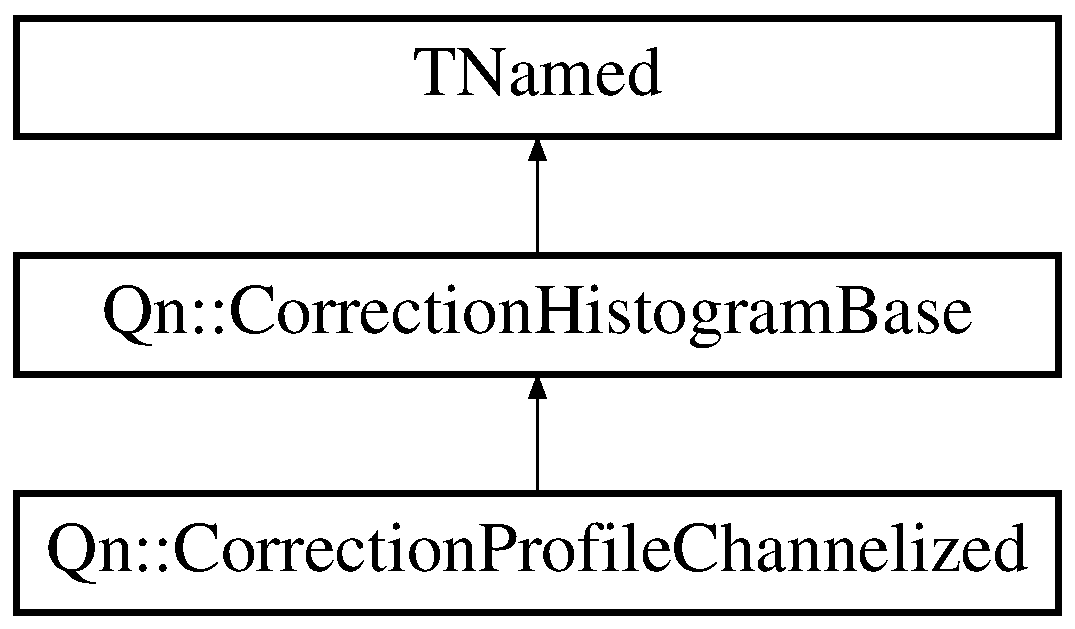
\includegraphics[height=3.000000cm]{classQn_1_1CorrectionProfileChannelized}
\end{center}
\end{figure}
\subsection*{Public Member Functions}
\begin{DoxyCompactItemize}
\item 
\mbox{\Hypertarget{classQn_1_1CorrectionProfileChannelized_a82745b91a442b1999b166dadf312b47d}\label{classQn_1_1CorrectionProfileChannelized_a82745b91a442b1999b166dadf312b47d}} 
\mbox{\hyperlink{classQn_1_1CorrectionProfileChannelized_a82745b91a442b1999b166dadf312b47d}{Correction\+Profile\+Channelized}} ()
\begin{DoxyCompactList}\small\item\em Default constructor. \end{DoxyCompactList}\item 
\mbox{\hyperlink{classQn_1_1CorrectionProfileChannelized_ad3860853ae13c35e17017767005cda92}{Correction\+Profile\+Channelized}} (const char $\ast$name, const char $\ast$title, \mbox{\hyperlink{classQn_1_1EventClassVariablesSet}{Event\+Class\+Variables\+Set}} \&ecvs, Int\+\_\+t n\+No\+Of\+Channels, Option\+\_\+t $\ast$option=\char`\"{}\char`\"{})
\item 
virtual \mbox{\hyperlink{classQn_1_1CorrectionProfileChannelized_a5389dfe26fc02d4efd276ae5b9dcd7b8}{$\sim$\+Correction\+Profile\+Channelized}} ()
\item 
Bool\+\_\+t \mbox{\hyperlink{classQn_1_1CorrectionProfileChannelized_ad98e4ab64dbbc306de3b67eee35a1425}{Create\+Profile\+Histograms}} (T\+List $\ast$histogram\+List, const Bool\+\_\+t $\ast$b\+Used\+Channel, const Int\+\_\+t $\ast$n\+Channel\+Group)
\item 
virtual Long64\+\_\+t \mbox{\hyperlink{classQn_1_1CorrectionProfileChannelized_a10eb9b98a847afecf08e01e4e82bd4c5}{Get\+Bin}} (const double $\ast$variable\+Container, Int\+\_\+t n\+Channel)
\item 
\mbox{\Hypertarget{classQn_1_1CorrectionProfileChannelized_aa495dacf1deb21e799a08afbefd323a3}\label{classQn_1_1CorrectionProfileChannelized_aa495dacf1deb21e799a08afbefd323a3}} 
virtual Long64\+\_\+t \mbox{\hyperlink{classQn_1_1CorrectionProfileChannelized_aa495dacf1deb21e799a08afbefd323a3}{Get\+Bin}} (const double $\ast$variable\+Container)
\begin{DoxyCompactList}\small\item\em wrong call for this class invoke base class behavior \end{DoxyCompactList}\item 
virtual Bool\+\_\+t \mbox{\hyperlink{classQn_1_1CorrectionProfileChannelized_a1a7640ed888a3357d28f3f0f8e8b4bec}{Bin\+Content\+Validated}} (Long64\+\_\+t bin)
\item 
virtual Float\+\_\+t \mbox{\hyperlink{classQn_1_1CorrectionProfileChannelized_a45d475d580d3c5dfe9d139552eab766b}{Get\+Bin\+Content}} (Long64\+\_\+t bin)
\item 
virtual Float\+\_\+t \mbox{\hyperlink{classQn_1_1CorrectionProfileChannelized_a68b390bb4d744453239bca73a1c3ca84}{Get\+Bin\+Error}} (Long64\+\_\+t bin)
\item 
virtual void \mbox{\hyperlink{classQn_1_1CorrectionProfileChannelized_a154acd464664786fc84177964072f55b}{Fill}} (const double $\ast$variable\+Container, Int\+\_\+t n\+Channel, Float\+\_\+t weight)
\item 
\mbox{\Hypertarget{classQn_1_1CorrectionProfileChannelized_ad063c82996e749fdf54526d3c627249b}\label{classQn_1_1CorrectionProfileChannelized_ad063c82996e749fdf54526d3c627249b}} 
virtual void \mbox{\hyperlink{classQn_1_1CorrectionProfileChannelized_ad063c82996e749fdf54526d3c627249b}{Fill}} (const double $\ast$variable\+Container, Float\+\_\+t weight)
\begin{DoxyCompactList}\small\item\em wrong call for this class invoke base class behavior \end{DoxyCompactList}\end{DoxyCompactItemize}
\subsection*{Additional Inherited Members}


\subsection{Constructor \& Destructor Documentation}
\mbox{\Hypertarget{classQn_1_1CorrectionProfileChannelized_ad3860853ae13c35e17017767005cda92}\label{classQn_1_1CorrectionProfileChannelized_ad3860853ae13c35e17017767005cda92}} 
\index{Qn\+::\+Correction\+Profile\+Channelized@{Qn\+::\+Correction\+Profile\+Channelized}!Correction\+Profile\+Channelized@{Correction\+Profile\+Channelized}}
\index{Correction\+Profile\+Channelized@{Correction\+Profile\+Channelized}!Qn\+::\+Correction\+Profile\+Channelized@{Qn\+::\+Correction\+Profile\+Channelized}}
\subsubsection{\texorpdfstring{Correction\+Profile\+Channelized()}{CorrectionProfileChannelized()}}
{\footnotesize\ttfamily Qn\+::\+Correction\+Profile\+Channelized\+::\+Correction\+Profile\+Channelized (\begin{DoxyParamCaption}\item[{const char $\ast$}]{name,  }\item[{const char $\ast$}]{title,  }\item[{\mbox{\hyperlink{classQn_1_1EventClassVariablesSet}{Event\+Class\+Variables\+Set}} \&}]{ecvs,  }\item[{Int\+\_\+t}]{n\+No\+Of\+Channels,  }\item[{Option\+\_\+t $\ast$}]{option = {\ttfamily \char`\"{}\char`\"{}} }\end{DoxyParamCaption})}

Normal constructor

Stores the set of variables that identify the different event classes passing them to its parent and prepares the object for actual histogram creation or attachment


\begin{DoxyParams}{Parameters}
{\em name} & base for the name of the histograms \\
\hline
{\em title} & base for the title of the histograms \\
\hline
{\em ecvs} & the event classes variables set \\
\hline
{\em n\+No\+Of\+Channels} & the number of channels associated \\
\hline
{\em option} & option for errors computation \textquotesingle{} \textquotesingle{} (Default) the bin errors are the standard error on the mean of the bin values\\
\hline
\end{DoxyParams}
\textquotesingle{}s\textquotesingle{} the bin are the standard deviation of of the bin values \mbox{\Hypertarget{classQn_1_1CorrectionProfileChannelized_a5389dfe26fc02d4efd276ae5b9dcd7b8}\label{classQn_1_1CorrectionProfileChannelized_a5389dfe26fc02d4efd276ae5b9dcd7b8}} 
\index{Qn\+::\+Correction\+Profile\+Channelized@{Qn\+::\+Correction\+Profile\+Channelized}!````~Correction\+Profile\+Channelized@{$\sim$\+Correction\+Profile\+Channelized}}
\index{````~Correction\+Profile\+Channelized@{$\sim$\+Correction\+Profile\+Channelized}!Qn\+::\+Correction\+Profile\+Channelized@{Qn\+::\+Correction\+Profile\+Channelized}}
\subsubsection{\texorpdfstring{$\sim$\+Correction\+Profile\+Channelized()}{~CorrectionProfileChannelized()}}
{\footnotesize\ttfamily Qn\+::\+Correction\+Profile\+Channelized\+::$\sim$\+Correction\+Profile\+Channelized (\begin{DoxyParamCaption}{ }\end{DoxyParamCaption})\hspace{0.3cm}{\ttfamily [virtual]}}

Default destructor Releases the memory taken 

\subsection{Member Function Documentation}
\mbox{\Hypertarget{classQn_1_1CorrectionProfileChannelized_a1a7640ed888a3357d28f3f0f8e8b4bec}\label{classQn_1_1CorrectionProfileChannelized_a1a7640ed888a3357d28f3f0f8e8b4bec}} 
\index{Qn\+::\+Correction\+Profile\+Channelized@{Qn\+::\+Correction\+Profile\+Channelized}!Bin\+Content\+Validated@{Bin\+Content\+Validated}}
\index{Bin\+Content\+Validated@{Bin\+Content\+Validated}!Qn\+::\+Correction\+Profile\+Channelized@{Qn\+::\+Correction\+Profile\+Channelized}}
\subsubsection{\texorpdfstring{Bin\+Content\+Validated()}{BinContentValidated()}}
{\footnotesize\ttfamily Bool\+\_\+t Qn\+::\+Correction\+Profile\+Channelized\+::\+Bin\+Content\+Validated (\begin{DoxyParamCaption}\item[{Long64\+\_\+t}]{bin }\end{DoxyParamCaption})\hspace{0.3cm}{\ttfamily [virtual]}}

Check the validity of the content of the passed bin If the number of entries is lower than the minimum number of entries to validate it the bin content is not considered valid and k\+F\+A\+L\+SE is returned, otherwise k\+T\+R\+UE is returned 
\begin{DoxyParams}{Parameters}
{\em bin} & the bin to check its content validity \\
\hline
\end{DoxyParams}
\begin{DoxyReturn}{Returns}
k\+T\+R\+UE if the content is valid k\+F\+A\+L\+SE otherwise 
\end{DoxyReturn}


Implements \mbox{\hyperlink{classQn_1_1CorrectionHistogramBase_a4db2c92ceaffefaa91475a721612d80d}{Qn\+::\+Correction\+Histogram\+Base}}.

\mbox{\Hypertarget{classQn_1_1CorrectionProfileChannelized_ad98e4ab64dbbc306de3b67eee35a1425}\label{classQn_1_1CorrectionProfileChannelized_ad98e4ab64dbbc306de3b67eee35a1425}} 
\index{Qn\+::\+Correction\+Profile\+Channelized@{Qn\+::\+Correction\+Profile\+Channelized}!Create\+Profile\+Histograms@{Create\+Profile\+Histograms}}
\index{Create\+Profile\+Histograms@{Create\+Profile\+Histograms}!Qn\+::\+Correction\+Profile\+Channelized@{Qn\+::\+Correction\+Profile\+Channelized}}
\subsubsection{\texorpdfstring{Create\+Profile\+Histograms()}{CreateProfileHistograms()}}
{\footnotesize\ttfamily Bool\+\_\+t Qn\+::\+Correction\+Profile\+Channelized\+::\+Create\+Profile\+Histograms (\begin{DoxyParamCaption}\item[{T\+List $\ast$}]{histogram\+List,  }\item[{const Bool\+\_\+t $\ast$}]{b\+Used\+Channel,  }\item[{const Int\+\_\+t $\ast$}]{n\+Channel\+Group }\end{DoxyParamCaption})}

Creates the support histograms for the profile function

Based in the event classes variables set in the parent class and the channel information passed as parameters the values and entries multidimensional histograms are created.

Both histograms are added to the passed histogram list

The actual number of channels is stored and a mask from external channel number to histogram channel number. If b\+Used\+Channel is N\+U\+LL all channels within f\+No\+Of\+Channels are assigned to this profile. If n\+Channel\+Group is N\+U\+LL all channels assigned to this profile are allocated to the same group. 
\begin{DoxyParams}{Parameters}
{\em histogram\+List} & list where the histograms have to be added \\
\hline
{\em b\+Used\+Channel} & array of booleans one per each channel \\
\hline
{\em n\+Channel\+Group} & array of group number for each channel \\
\hline
\end{DoxyParams}
\begin{DoxyReturn}{Returns}
true if properly created 
\end{DoxyReturn}
\mbox{\Hypertarget{classQn_1_1CorrectionProfileChannelized_a154acd464664786fc84177964072f55b}\label{classQn_1_1CorrectionProfileChannelized_a154acd464664786fc84177964072f55b}} 
\index{Qn\+::\+Correction\+Profile\+Channelized@{Qn\+::\+Correction\+Profile\+Channelized}!Fill@{Fill}}
\index{Fill@{Fill}!Qn\+::\+Correction\+Profile\+Channelized@{Qn\+::\+Correction\+Profile\+Channelized}}
\subsubsection{\texorpdfstring{Fill()}{Fill()}}
{\footnotesize\ttfamily void Qn\+::\+Correction\+Profile\+Channelized\+::\+Fill (\begin{DoxyParamCaption}\item[{const double $\ast$}]{variable\+Container,  }\item[{Int\+\_\+t}]{n\+Channel,  }\item[{Float\+\_\+t}]{weight }\end{DoxyParamCaption})\hspace{0.3cm}{\ttfamily [virtual]}}

Fills the histogram

The involved bin is computed according to the current variables content and the passed external channel number. The bin is then increased by the given weight and the entries also increased properly.


\begin{DoxyParams}{Parameters}
{\em variable\+Container} & the current variables content addressed by var Id \\
\hline
{\em n\+Channel} & the interested external channel number \\
\hline
{\em weight} & the increment in the bin content \\
\hline
\end{DoxyParams}


Reimplemented from \mbox{\hyperlink{classQn_1_1CorrectionHistogramBase_ae94b20c7d396f5b179fb11d84d764c09}{Qn\+::\+Correction\+Histogram\+Base}}.

\mbox{\Hypertarget{classQn_1_1CorrectionProfileChannelized_a10eb9b98a847afecf08e01e4e82bd4c5}\label{classQn_1_1CorrectionProfileChannelized_a10eb9b98a847afecf08e01e4e82bd4c5}} 
\index{Qn\+::\+Correction\+Profile\+Channelized@{Qn\+::\+Correction\+Profile\+Channelized}!Get\+Bin@{Get\+Bin}}
\index{Get\+Bin@{Get\+Bin}!Qn\+::\+Correction\+Profile\+Channelized@{Qn\+::\+Correction\+Profile\+Channelized}}
\subsubsection{\texorpdfstring{Get\+Bin()}{GetBin()}}
{\footnotesize\ttfamily Long64\+\_\+t Qn\+::\+Correction\+Profile\+Channelized\+::\+Get\+Bin (\begin{DoxyParamCaption}\item[{const double $\ast$}]{variable\+Container,  }\item[{Int\+\_\+t}]{n\+Channel }\end{DoxyParamCaption})\hspace{0.3cm}{\ttfamily [virtual]}}

Get the bin number for the current variable content and passed channel

The bin number identifies the event class the current variable content points to under the passed channel.


\begin{DoxyParams}{Parameters}
{\em variable\+Container} & the current variables content addressed by var Id \\
\hline
{\em n\+Channel} & the interested external channel number \\
\hline
\end{DoxyParams}
\begin{DoxyReturn}{Returns}
the associated bin to the current variables content 
\end{DoxyReturn}


Reimplemented from \mbox{\hyperlink{classQn_1_1CorrectionHistogramBase_acfde166908e4da950470841f21f87fb9}{Qn\+::\+Correction\+Histogram\+Base}}.

\mbox{\Hypertarget{classQn_1_1CorrectionProfileChannelized_a45d475d580d3c5dfe9d139552eab766b}\label{classQn_1_1CorrectionProfileChannelized_a45d475d580d3c5dfe9d139552eab766b}} 
\index{Qn\+::\+Correction\+Profile\+Channelized@{Qn\+::\+Correction\+Profile\+Channelized}!Get\+Bin\+Content@{Get\+Bin\+Content}}
\index{Get\+Bin\+Content@{Get\+Bin\+Content}!Qn\+::\+Correction\+Profile\+Channelized@{Qn\+::\+Correction\+Profile\+Channelized}}
\subsubsection{\texorpdfstring{Get\+Bin\+Content()}{GetBinContent()}}
{\footnotesize\ttfamily Float\+\_\+t Qn\+::\+Correction\+Profile\+Channelized\+::\+Get\+Bin\+Content (\begin{DoxyParamCaption}\item[{Long64\+\_\+t}]{bin }\end{DoxyParamCaption})\hspace{0.3cm}{\ttfamily [virtual]}}

Get the bin content for the passed bin number

The bin number identifies a desired event class whose content is requested. If the bin content is not validated zero is returned.


\begin{DoxyParams}{Parameters}
{\em bin} & the interested bin number \\
\hline
\end{DoxyParams}
\begin{DoxyReturn}{Returns}
the bin number content 
\end{DoxyReturn}


Reimplemented from \mbox{\hyperlink{classQn_1_1CorrectionHistogramBase_a9e4e745a6f4cbebf5b9277d6d63bc9c7}{Qn\+::\+Correction\+Histogram\+Base}}.

\mbox{\Hypertarget{classQn_1_1CorrectionProfileChannelized_a68b390bb4d744453239bca73a1c3ca84}\label{classQn_1_1CorrectionProfileChannelized_a68b390bb4d744453239bca73a1c3ca84}} 
\index{Qn\+::\+Correction\+Profile\+Channelized@{Qn\+::\+Correction\+Profile\+Channelized}!Get\+Bin\+Error@{Get\+Bin\+Error}}
\index{Get\+Bin\+Error@{Get\+Bin\+Error}!Qn\+::\+Correction\+Profile\+Channelized@{Qn\+::\+Correction\+Profile\+Channelized}}
\subsubsection{\texorpdfstring{Get\+Bin\+Error()}{GetBinError()}}
{\footnotesize\ttfamily Float\+\_\+t Qn\+::\+Correction\+Profile\+Channelized\+::\+Get\+Bin\+Error (\begin{DoxyParamCaption}\item[{Long64\+\_\+t}]{bin }\end{DoxyParamCaption})\hspace{0.3cm}{\ttfamily [virtual]}}

Get the bin content error for the passed bin number

The bin number identifies a desired event class whose content error is requested. If the bin content is not validated zero is returned.


\begin{DoxyParams}{Parameters}
{\em bin} & the interested bin number \\
\hline
\end{DoxyParams}
\begin{DoxyReturn}{Returns}
the bin number content error 
\end{DoxyReturn}


Reimplemented from \mbox{\hyperlink{classQn_1_1CorrectionHistogramBase_a50a7dd4c5bbe5e4d0e405365c2a9104d}{Qn\+::\+Correction\+Histogram\+Base}}.



The documentation for this class was generated from the following files\+:\begin{DoxyCompactItemize}
\item 
D\+T\+\_\+\+Flow/\+Qn\+Corrections/include/Correction\+Profile\+Channelized.\+h\item 
D\+T\+\_\+\+Flow/\+Qn\+Corrections/Correction\+Profile\+Channelized.\+cpp\end{DoxyCompactItemize}

\hypertarget{classQn_1_1CorrectionProfileChannelizedIngress}{}\section{Qn\+:\+:Correction\+Profile\+Channelized\+Ingress Class Reference}
\label{classQn_1_1CorrectionProfileChannelizedIngress}\index{Qn\+::\+Correction\+Profile\+Channelized\+Ingress@{Qn\+::\+Correction\+Profile\+Channelized\+Ingress}}
Inheritance diagram for Qn\+:\+:Correction\+Profile\+Channelized\+Ingress\+:\begin{figure}[H]
\begin{center}
\leavevmode
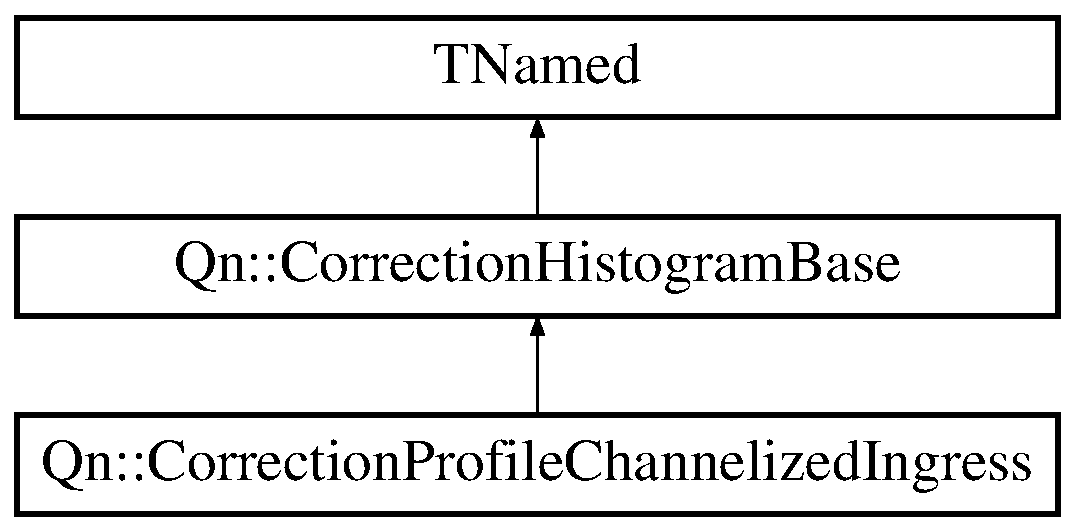
\includegraphics[height=3.000000cm]{classQn_1_1CorrectionProfileChannelizedIngress}
\end{center}
\end{figure}
\subsection*{Public Member Functions}
\begin{DoxyCompactItemize}
\item 
\mbox{\Hypertarget{classQn_1_1CorrectionProfileChannelizedIngress_a659be643e7bf23a8a3d791092981b2a2}\label{classQn_1_1CorrectionProfileChannelizedIngress_a659be643e7bf23a8a3d791092981b2a2}} 
\mbox{\hyperlink{classQn_1_1CorrectionProfileChannelizedIngress_a659be643e7bf23a8a3d791092981b2a2}{Correction\+Profile\+Channelized\+Ingress}} ()
\begin{DoxyCompactList}\small\item\em Default constructor. \end{DoxyCompactList}\item 
\mbox{\hyperlink{classQn_1_1CorrectionProfileChannelizedIngress_a9afde955744af4075b927913246ec065}{Correction\+Profile\+Channelized\+Ingress}} (const char $\ast$name, const char $\ast$title, \mbox{\hyperlink{classQn_1_1EventClassVariablesSet}{Event\+Class\+Variables\+Set}} \&ecvs, Int\+\_\+t n\+No\+Of\+Channels, Option\+\_\+t $\ast$option=\char`\"{}\char`\"{})
\item 
virtual \mbox{\hyperlink{classQn_1_1CorrectionProfileChannelizedIngress_a141b89a1b38a9b16023a9dc413a9be05}{$\sim$\+Correction\+Profile\+Channelized\+Ingress}} ()
\item 
virtual Bool\+\_\+t \mbox{\hyperlink{classQn_1_1CorrectionProfileChannelizedIngress_a770f44f4c5e700a71eb5a2cf5edab1a2}{Attach\+Histograms}} (T\+List $\ast$histogram\+List, const Bool\+\_\+t $\ast$b\+Used\+Channel, const Int\+\_\+t $\ast$n\+Channel\+Group)
\item 
\mbox{\Hypertarget{classQn_1_1CorrectionProfileChannelizedIngress_a98ef1bc824701a5e2eb5deb20a6c524f}\label{classQn_1_1CorrectionProfileChannelizedIngress_a98ef1bc824701a5e2eb5deb20a6c524f}} 
virtual Bool\+\_\+t \mbox{\hyperlink{classQn_1_1CorrectionProfileChannelizedIngress_a98ef1bc824701a5e2eb5deb20a6c524f}{Attach\+Histograms}} (T\+List $\ast$histogram\+List)
\begin{DoxyCompactList}\small\item\em wrong call for this class invoke base class behavior \end{DoxyCompactList}\item 
virtual Long64\+\_\+t \mbox{\hyperlink{classQn_1_1CorrectionProfileChannelizedIngress_aa9e937955e58199dedc3a75e5d593aa2}{Get\+Bin}} (const double $\ast$variable\+Container, Int\+\_\+t n\+Channel)
\item 
virtual Long64\+\_\+t \mbox{\hyperlink{classQn_1_1CorrectionProfileChannelizedIngress_aa28e227c6ba5d7c8ecc03b9c4180a523}{Get\+Grp\+Bin}} (const double $\ast$variable\+Container, Int\+\_\+t n\+Channel)
\item 
\mbox{\Hypertarget{classQn_1_1CorrectionProfileChannelizedIngress_a2716e7f057235fecd959ca967c29fd63}\label{classQn_1_1CorrectionProfileChannelizedIngress_a2716e7f057235fecd959ca967c29fd63}} 
virtual Long64\+\_\+t \mbox{\hyperlink{classQn_1_1CorrectionProfileChannelizedIngress_a2716e7f057235fecd959ca967c29fd63}{Get\+Bin}} (const double $\ast$variable\+Container)
\begin{DoxyCompactList}\small\item\em wrong call for this class invoke base class behavior \end{DoxyCompactList}\item 
virtual Bool\+\_\+t \mbox{\hyperlink{classQn_1_1CorrectionProfileChannelizedIngress_ad21ca0cea3bb64b832da59a99da2603a}{Bin\+Content\+Validated}} (Long64\+\_\+t bin)
\item 
virtual Float\+\_\+t \mbox{\hyperlink{classQn_1_1CorrectionProfileChannelizedIngress_a64fbd6f89e6ddcb0ef22189e868594fa}{Get\+Bin\+Content}} (Long64\+\_\+t bin)
\item 
virtual Float\+\_\+t \mbox{\hyperlink{classQn_1_1CorrectionProfileChannelizedIngress_ae150d82ad7a8b0cdc830dd41b46296ed}{Get\+Grp\+Bin\+Content}} (Long64\+\_\+t bin)
\item 
virtual Float\+\_\+t \mbox{\hyperlink{classQn_1_1CorrectionProfileChannelizedIngress_ace03557cdc8d3f87637b0f4108308cc0}{Get\+Bin\+Error}} (Long64\+\_\+t bin)
\item 
virtual Float\+\_\+t \mbox{\hyperlink{classQn_1_1CorrectionProfileChannelizedIngress_acc740b3b8325d5e0604a1826edbf6085}{Get\+Grp\+Bin\+Error}} (Long64\+\_\+t bin)
\end{DoxyCompactItemize}
\subsection*{Additional Inherited Members}


\subsection{Constructor \& Destructor Documentation}
\mbox{\Hypertarget{classQn_1_1CorrectionProfileChannelizedIngress_a9afde955744af4075b927913246ec065}\label{classQn_1_1CorrectionProfileChannelizedIngress_a9afde955744af4075b927913246ec065}} 
\index{Qn\+::\+Correction\+Profile\+Channelized\+Ingress@{Qn\+::\+Correction\+Profile\+Channelized\+Ingress}!Correction\+Profile\+Channelized\+Ingress@{Correction\+Profile\+Channelized\+Ingress}}
\index{Correction\+Profile\+Channelized\+Ingress@{Correction\+Profile\+Channelized\+Ingress}!Qn\+::\+Correction\+Profile\+Channelized\+Ingress@{Qn\+::\+Correction\+Profile\+Channelized\+Ingress}}
\subsubsection{\texorpdfstring{Correction\+Profile\+Channelized\+Ingress()}{CorrectionProfileChannelizedIngress()}}
{\footnotesize\ttfamily Qn\+::\+Correction\+Profile\+Channelized\+Ingress\+::\+Correction\+Profile\+Channelized\+Ingress (\begin{DoxyParamCaption}\item[{const char $\ast$}]{name,  }\item[{const char $\ast$}]{title,  }\item[{\mbox{\hyperlink{classQn_1_1EventClassVariablesSet}{Event\+Class\+Variables\+Set}} \&}]{ecvs,  }\item[{Int\+\_\+t}]{n\+No\+Of\+Channels,  }\item[{Option\+\_\+t $\ast$}]{option = {\ttfamily \char`\"{}\char`\"{}} }\end{DoxyParamCaption})}

Normal constructor

Stores the set of variables that identify the different event classes passing them to its parent and prepares the object for actual histogram attachment


\begin{DoxyParams}{Parameters}
{\em name} & base for the name of the histograms \\
\hline
{\em title} & base for the title of the histograms \\
\hline
{\em ecvs} & the event classes variables set \\
\hline
{\em n\+No\+Of\+Channels} & the number of channels associated \\
\hline
{\em option} & option for errors computation \textquotesingle{} \textquotesingle{} (Default) the bin errors are the standard error on the mean of the bin values\\
\hline
\end{DoxyParams}
\textquotesingle{}s\textquotesingle{} the bin are the standard deviation of of the bin values \mbox{\Hypertarget{classQn_1_1CorrectionProfileChannelizedIngress_a141b89a1b38a9b16023a9dc413a9be05}\label{classQn_1_1CorrectionProfileChannelizedIngress_a141b89a1b38a9b16023a9dc413a9be05}} 
\index{Qn\+::\+Correction\+Profile\+Channelized\+Ingress@{Qn\+::\+Correction\+Profile\+Channelized\+Ingress}!````~Correction\+Profile\+Channelized\+Ingress@{$\sim$\+Correction\+Profile\+Channelized\+Ingress}}
\index{````~Correction\+Profile\+Channelized\+Ingress@{$\sim$\+Correction\+Profile\+Channelized\+Ingress}!Qn\+::\+Correction\+Profile\+Channelized\+Ingress@{Qn\+::\+Correction\+Profile\+Channelized\+Ingress}}
\subsubsection{\texorpdfstring{$\sim$\+Correction\+Profile\+Channelized\+Ingress()}{~CorrectionProfileChannelizedIngress()}}
{\footnotesize\ttfamily Qn\+::\+Correction\+Profile\+Channelized\+Ingress\+::$\sim$\+Correction\+Profile\+Channelized\+Ingress (\begin{DoxyParamCaption}{ }\end{DoxyParamCaption})\hspace{0.3cm}{\ttfamily [virtual]}}

Default destructor Releases the memory taken 

\subsection{Member Function Documentation}
\mbox{\Hypertarget{classQn_1_1CorrectionProfileChannelizedIngress_a770f44f4c5e700a71eb5a2cf5edab1a2}\label{classQn_1_1CorrectionProfileChannelizedIngress_a770f44f4c5e700a71eb5a2cf5edab1a2}} 
\index{Qn\+::\+Correction\+Profile\+Channelized\+Ingress@{Qn\+::\+Correction\+Profile\+Channelized\+Ingress}!Attach\+Histograms@{Attach\+Histograms}}
\index{Attach\+Histograms@{Attach\+Histograms}!Qn\+::\+Correction\+Profile\+Channelized\+Ingress@{Qn\+::\+Correction\+Profile\+Channelized\+Ingress}}
\subsubsection{\texorpdfstring{Attach\+Histograms()}{AttachHistograms()}}
{\footnotesize\ttfamily Bool\+\_\+t Qn\+::\+Correction\+Profile\+Channelized\+Ingress\+::\+Attach\+Histograms (\begin{DoxyParamCaption}\item[{T\+List $\ast$}]{histogram\+List,  }\item[{const Bool\+\_\+t $\ast$}]{b\+Used\+Channel,  }\item[{const Int\+\_\+t $\ast$}]{n\+Channel\+Group }\end{DoxyParamCaption})\hspace{0.3cm}{\ttfamily [virtual]}}

Attaches existing histograms as the support histograms for the profile function

The histograms are located in the passed list and if found and with the proper dimensions their references are stored in member variables.

Channel information is used to build internal structures such as the channel map and the actual number of channels and the channels groups and the actual number of groups. The information is matched with the found histogram to validate it. If b\+Used\+Channel is N\+U\+LL all channels within f\+No\+Of\+Channels are assigned to this profile. If n\+Channel\+Group is N\+U\+LL all channels assigned to this profile are allocated to the same group.

Once the histograms are found and validated, a unique value / error channel histogram is created for efficient access and a potential unique value / error channels group histogram is created. 
\begin{DoxyParams}{Parameters}
{\em histogram\+List} & list where the histograms have to be located \\
\hline
{\em b\+Used\+Channel} & array of booleans one per each channel \\
\hline
{\em n\+Channel\+Group} & array of group number for each channel \\
\hline
\end{DoxyParams}
\begin{DoxyReturn}{Returns}
true if properly attached else false 
\end{DoxyReturn}


Reimplemented from \mbox{\hyperlink{classQn_1_1CorrectionHistogramBase_afa979697b43e2ebd0580a3359b2aca63}{Qn\+::\+Correction\+Histogram\+Base}}.

\mbox{\Hypertarget{classQn_1_1CorrectionProfileChannelizedIngress_ad21ca0cea3bb64b832da59a99da2603a}\label{classQn_1_1CorrectionProfileChannelizedIngress_ad21ca0cea3bb64b832da59a99da2603a}} 
\index{Qn\+::\+Correction\+Profile\+Channelized\+Ingress@{Qn\+::\+Correction\+Profile\+Channelized\+Ingress}!Bin\+Content\+Validated@{Bin\+Content\+Validated}}
\index{Bin\+Content\+Validated@{Bin\+Content\+Validated}!Qn\+::\+Correction\+Profile\+Channelized\+Ingress@{Qn\+::\+Correction\+Profile\+Channelized\+Ingress}}
\subsubsection{\texorpdfstring{Bin\+Content\+Validated()}{BinContentValidated()}}
{\footnotesize\ttfamily Bool\+\_\+t Qn\+::\+Correction\+Profile\+Channelized\+Ingress\+::\+Bin\+Content\+Validated (\begin{DoxyParamCaption}\item[{Long64\+\_\+t}]{bin }\end{DoxyParamCaption})\hspace{0.3cm}{\ttfamily [virtual]}}

Check the validity of the content of the passed bin For the time being this kind of histograms cannot check bin content validity so, k\+T\+R\+UE is returned. 
\begin{DoxyParams}{Parameters}
{\em bin} & the bin to check its content validity \\
\hline
\end{DoxyParams}
\begin{DoxyReturn}{Returns}
k\+T\+R\+UE if the content is valid k\+F\+A\+L\+SE otherwise 
\end{DoxyReturn}


Implements \mbox{\hyperlink{classQn_1_1CorrectionHistogramBase_a4db2c92ceaffefaa91475a721612d80d}{Qn\+::\+Correction\+Histogram\+Base}}.

\mbox{\Hypertarget{classQn_1_1CorrectionProfileChannelizedIngress_aa9e937955e58199dedc3a75e5d593aa2}\label{classQn_1_1CorrectionProfileChannelizedIngress_aa9e937955e58199dedc3a75e5d593aa2}} 
\index{Qn\+::\+Correction\+Profile\+Channelized\+Ingress@{Qn\+::\+Correction\+Profile\+Channelized\+Ingress}!Get\+Bin@{Get\+Bin}}
\index{Get\+Bin@{Get\+Bin}!Qn\+::\+Correction\+Profile\+Channelized\+Ingress@{Qn\+::\+Correction\+Profile\+Channelized\+Ingress}}
\subsubsection{\texorpdfstring{Get\+Bin()}{GetBin()}}
{\footnotesize\ttfamily Long64\+\_\+t Qn\+::\+Correction\+Profile\+Channelized\+Ingress\+::\+Get\+Bin (\begin{DoxyParamCaption}\item[{const double $\ast$}]{variable\+Container,  }\item[{Int\+\_\+t}]{n\+Channel }\end{DoxyParamCaption})\hspace{0.3cm}{\ttfamily [virtual]}}

Get the bin number for the current variable content and passed channel

The bin number identifies the event class the current variable content points to under the passed channel.


\begin{DoxyParams}{Parameters}
{\em variable\+Container} & the current variables content addressed by var Id \\
\hline
{\em n\+Channel} & the interested external channel number \\
\hline
\end{DoxyParams}
\begin{DoxyReturn}{Returns}
the associated bin to the current variables content 
\end{DoxyReturn}


Reimplemented from \mbox{\hyperlink{classQn_1_1CorrectionHistogramBase_acfde166908e4da950470841f21f87fb9}{Qn\+::\+Correction\+Histogram\+Base}}.

\mbox{\Hypertarget{classQn_1_1CorrectionProfileChannelizedIngress_a64fbd6f89e6ddcb0ef22189e868594fa}\label{classQn_1_1CorrectionProfileChannelizedIngress_a64fbd6f89e6ddcb0ef22189e868594fa}} 
\index{Qn\+::\+Correction\+Profile\+Channelized\+Ingress@{Qn\+::\+Correction\+Profile\+Channelized\+Ingress}!Get\+Bin\+Content@{Get\+Bin\+Content}}
\index{Get\+Bin\+Content@{Get\+Bin\+Content}!Qn\+::\+Correction\+Profile\+Channelized\+Ingress@{Qn\+::\+Correction\+Profile\+Channelized\+Ingress}}
\subsubsection{\texorpdfstring{Get\+Bin\+Content()}{GetBinContent()}}
{\footnotesize\ttfamily Float\+\_\+t Qn\+::\+Correction\+Profile\+Channelized\+Ingress\+::\+Get\+Bin\+Content (\begin{DoxyParamCaption}\item[{Long64\+\_\+t}]{bin }\end{DoxyParamCaption})\hspace{0.3cm}{\ttfamily [virtual]}}

Get the bin content for the passed bin number

The bin number identifies a desired event class whose content is requested. The bin average stored as bin content is returned


\begin{DoxyParams}{Parameters}
{\em bin} & the interested bin number \\
\hline
\end{DoxyParams}
\begin{DoxyReturn}{Returns}
the bin number content 
\end{DoxyReturn}


Reimplemented from \mbox{\hyperlink{classQn_1_1CorrectionHistogramBase_a9e4e745a6f4cbebf5b9277d6d63bc9c7}{Qn\+::\+Correction\+Histogram\+Base}}.

\mbox{\Hypertarget{classQn_1_1CorrectionProfileChannelizedIngress_ace03557cdc8d3f87637b0f4108308cc0}\label{classQn_1_1CorrectionProfileChannelizedIngress_ace03557cdc8d3f87637b0f4108308cc0}} 
\index{Qn\+::\+Correction\+Profile\+Channelized\+Ingress@{Qn\+::\+Correction\+Profile\+Channelized\+Ingress}!Get\+Bin\+Error@{Get\+Bin\+Error}}
\index{Get\+Bin\+Error@{Get\+Bin\+Error}!Qn\+::\+Correction\+Profile\+Channelized\+Ingress@{Qn\+::\+Correction\+Profile\+Channelized\+Ingress}}
\subsubsection{\texorpdfstring{Get\+Bin\+Error()}{GetBinError()}}
{\footnotesize\ttfamily Float\+\_\+t Qn\+::\+Correction\+Profile\+Channelized\+Ingress\+::\+Get\+Bin\+Error (\begin{DoxyParamCaption}\item[{Long64\+\_\+t}]{bin }\end{DoxyParamCaption})\hspace{0.3cm}{\ttfamily [virtual]}}

Get the bin content error for the passed bin number

The bin number identifies a desired event class whose content error is requested. The bin error stored as bin error is returned.


\begin{DoxyParams}{Parameters}
{\em bin} & the interested bin number \\
\hline
\end{DoxyParams}
\begin{DoxyReturn}{Returns}
the bin number content error 
\end{DoxyReturn}


Reimplemented from \mbox{\hyperlink{classQn_1_1CorrectionHistogramBase_a50a7dd4c5bbe5e4d0e405365c2a9104d}{Qn\+::\+Correction\+Histogram\+Base}}.

\mbox{\Hypertarget{classQn_1_1CorrectionProfileChannelizedIngress_aa28e227c6ba5d7c8ecc03b9c4180a523}\label{classQn_1_1CorrectionProfileChannelizedIngress_aa28e227c6ba5d7c8ecc03b9c4180a523}} 
\index{Qn\+::\+Correction\+Profile\+Channelized\+Ingress@{Qn\+::\+Correction\+Profile\+Channelized\+Ingress}!Get\+Grp\+Bin@{Get\+Grp\+Bin}}
\index{Get\+Grp\+Bin@{Get\+Grp\+Bin}!Qn\+::\+Correction\+Profile\+Channelized\+Ingress@{Qn\+::\+Correction\+Profile\+Channelized\+Ingress}}
\subsubsection{\texorpdfstring{Get\+Grp\+Bin()}{GetGrpBin()}}
{\footnotesize\ttfamily Long64\+\_\+t Qn\+::\+Correction\+Profile\+Channelized\+Ingress\+::\+Get\+Grp\+Bin (\begin{DoxyParamCaption}\item[{const double $\ast$}]{variable\+Container,  }\item[{Int\+\_\+t}]{n\+Channel }\end{DoxyParamCaption})\hspace{0.3cm}{\ttfamily [virtual]}}

Get the bin number for the current variable content and passed channel group number

The bin number identifies the event class the current variable content points to under the passed channel group number.


\begin{DoxyParams}{Parameters}
{\em variable\+Container} & the current variables content addressed by var Id \\
\hline
{\em n\+Channel} & the interested external channel number which group number is asked \\
\hline
\end{DoxyParams}
\begin{DoxyReturn}{Returns}
the associated bin to the current variables content 
\end{DoxyReturn}
\mbox{\Hypertarget{classQn_1_1CorrectionProfileChannelizedIngress_ae150d82ad7a8b0cdc830dd41b46296ed}\label{classQn_1_1CorrectionProfileChannelizedIngress_ae150d82ad7a8b0cdc830dd41b46296ed}} 
\index{Qn\+::\+Correction\+Profile\+Channelized\+Ingress@{Qn\+::\+Correction\+Profile\+Channelized\+Ingress}!Get\+Grp\+Bin\+Content@{Get\+Grp\+Bin\+Content}}
\index{Get\+Grp\+Bin\+Content@{Get\+Grp\+Bin\+Content}!Qn\+::\+Correction\+Profile\+Channelized\+Ingress@{Qn\+::\+Correction\+Profile\+Channelized\+Ingress}}
\subsubsection{\texorpdfstring{Get\+Grp\+Bin\+Content()}{GetGrpBinContent()}}
{\footnotesize\ttfamily Float\+\_\+t Qn\+::\+Correction\+Profile\+Channelized\+Ingress\+::\+Get\+Grp\+Bin\+Content (\begin{DoxyParamCaption}\item[{Long64\+\_\+t}]{bin }\end{DoxyParamCaption})\hspace{0.3cm}{\ttfamily [virtual]}}

Get the group bin content for the passed bin number

The bin number identifies a desired event class whose group content is requested.


\begin{DoxyParams}{Parameters}
{\em bin} & the interested group bin number \\
\hline
\end{DoxyParams}
\begin{DoxyReturn}{Returns}
the group bin number content 
\end{DoxyReturn}
\mbox{\Hypertarget{classQn_1_1CorrectionProfileChannelizedIngress_acc740b3b8325d5e0604a1826edbf6085}\label{classQn_1_1CorrectionProfileChannelizedIngress_acc740b3b8325d5e0604a1826edbf6085}} 
\index{Qn\+::\+Correction\+Profile\+Channelized\+Ingress@{Qn\+::\+Correction\+Profile\+Channelized\+Ingress}!Get\+Grp\+Bin\+Error@{Get\+Grp\+Bin\+Error}}
\index{Get\+Grp\+Bin\+Error@{Get\+Grp\+Bin\+Error}!Qn\+::\+Correction\+Profile\+Channelized\+Ingress@{Qn\+::\+Correction\+Profile\+Channelized\+Ingress}}
\subsubsection{\texorpdfstring{Get\+Grp\+Bin\+Error()}{GetGrpBinError()}}
{\footnotesize\ttfamily Float\+\_\+t Qn\+::\+Correction\+Profile\+Channelized\+Ingress\+::\+Get\+Grp\+Bin\+Error (\begin{DoxyParamCaption}\item[{Long64\+\_\+t}]{bin }\end{DoxyParamCaption})\hspace{0.3cm}{\ttfamily [virtual]}}

Get the group bin content error for the passed bin number

The group bin number identifies a desired event class whose content error is requested.


\begin{DoxyParams}{Parameters}
{\em bin} & the interested group bin number \\
\hline
\end{DoxyParams}
\begin{DoxyReturn}{Returns}
the bin number content error 
\end{DoxyReturn}


The documentation for this class was generated from the following files\+:\begin{DoxyCompactItemize}
\item 
D\+T\+\_\+\+Flow/\+Qn\+Corrections/include/Correction\+Profile\+Channelized\+Ingress.\+h\item 
D\+T\+\_\+\+Flow/\+Qn\+Corrections/Correction\+Profile\+Channelized\+Ingress.\+cpp\end{DoxyCompactItemize}

\hypertarget{classQn_1_1CorrectionProfileComponents}{}\section{Qn\+:\+:Correction\+Profile\+Components Class Reference}
\label{classQn_1_1CorrectionProfileComponents}\index{Qn\+::\+Correction\+Profile\+Components@{Qn\+::\+Correction\+Profile\+Components}}
Inheritance diagram for Qn\+:\+:Correction\+Profile\+Components\+:\begin{figure}[H]
\begin{center}
\leavevmode
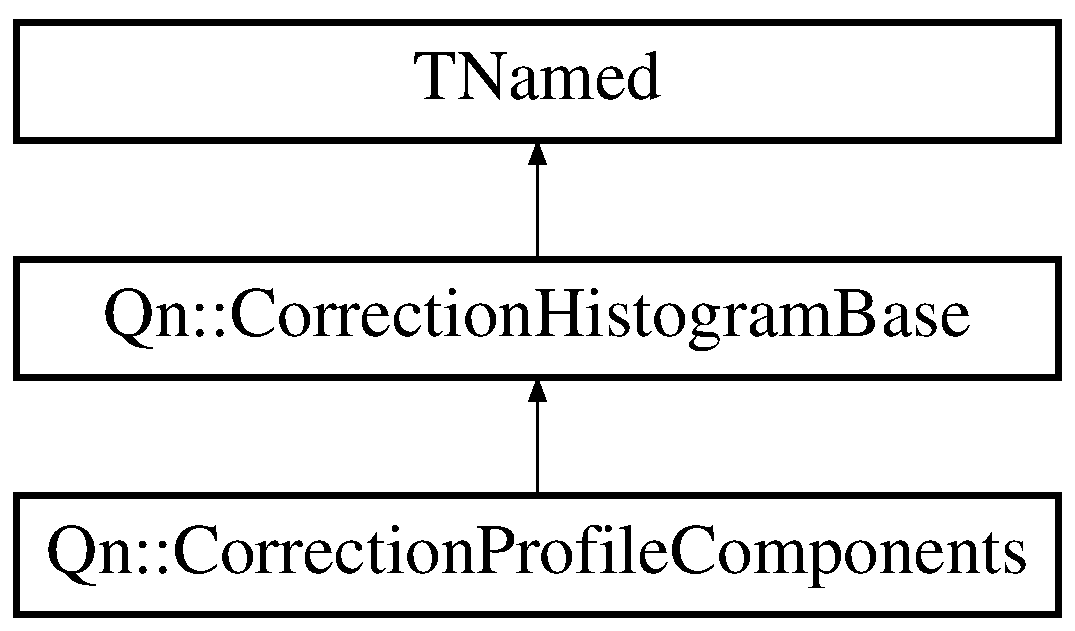
\includegraphics[height=3.000000cm]{classQn_1_1CorrectionProfileComponents}
\end{center}
\end{figure}
\subsection*{Public Member Functions}
\begin{DoxyCompactItemize}
\item 
\mbox{\Hypertarget{classQn_1_1CorrectionProfileComponents_ab682b61821f6efad703fb2043b92c086}\label{classQn_1_1CorrectionProfileComponents_ab682b61821f6efad703fb2043b92c086}} 
\mbox{\hyperlink{classQn_1_1CorrectionProfileComponents_ab682b61821f6efad703fb2043b92c086}{Correction\+Profile\+Components}} ()
\begin{DoxyCompactList}\small\item\em Default constructor. \end{DoxyCompactList}\item 
\mbox{\hyperlink{classQn_1_1CorrectionProfileComponents_afb4978830f231d9eeff316e013e7d07e}{Correction\+Profile\+Components}} (const char $\ast$name, const char $\ast$title, \mbox{\hyperlink{classQn_1_1EventClassVariablesSet}{Event\+Class\+Variables\+Set}} \&ecvs, Option\+\_\+t $\ast$option=\char`\"{}\char`\"{})
\item 
virtual \mbox{\hyperlink{classQn_1_1CorrectionProfileComponents_aefaf9152720bce6f1f9172c38732e90c}{$\sim$\+Correction\+Profile\+Components}} ()
\item 
Bool\+\_\+t \mbox{\hyperlink{classQn_1_1CorrectionProfileComponents_a4f965b6d5d75fac426b94210b0e3bec1}{Create\+Components\+Profile\+Histograms}} (T\+List $\ast$histogram\+List, Int\+\_\+t n\+No\+Of\+Harmonics, Int\+\_\+t $\ast$harmonic\+Map=N\+U\+LL)
\item 
virtual Bool\+\_\+t \mbox{\hyperlink{classQn_1_1CorrectionProfileComponents_adefa34cb026125ea0d52966c470f81af}{Attach\+Histograms}} (T\+List $\ast$histogram\+List)
\item 
\mbox{\Hypertarget{classQn_1_1CorrectionProfileComponents_a5b162699ea0d37e4c41af546285b476c}\label{classQn_1_1CorrectionProfileComponents_a5b162699ea0d37e4c41af546285b476c}} 
virtual Bool\+\_\+t \mbox{\hyperlink{classQn_1_1CorrectionProfileComponents_a5b162699ea0d37e4c41af546285b476c}{Attach\+Histograms}} (T\+List $\ast$histogram\+List, const Bool\+\_\+t $\ast$b\+Used\+Channel, const Int\+\_\+t $\ast$n\+Channel\+Group)
\begin{DoxyCompactList}\small\item\em wrong call for this class invoke base class behavior \end{DoxyCompactList}\item 
virtual Long64\+\_\+t \mbox{\hyperlink{classQn_1_1CorrectionProfileComponents_a379eff8f5c5b741e41fb70354a665ae2}{Get\+Bin}} (const double $\ast$variable\+Container)
\item 
\mbox{\Hypertarget{classQn_1_1CorrectionProfileComponents_ad3899de482c6f1f6a32d317b76e87a8a}\label{classQn_1_1CorrectionProfileComponents_ad3899de482c6f1f6a32d317b76e87a8a}} 
virtual Long64\+\_\+t \mbox{\hyperlink{classQn_1_1CorrectionProfileComponents_ad3899de482c6f1f6a32d317b76e87a8a}{Get\+Bin}} (const double $\ast$variable\+Container, Int\+\_\+t n\+Channel)
\begin{DoxyCompactList}\small\item\em wrong call for this class invoke base class behavior \end{DoxyCompactList}\item 
virtual Bool\+\_\+t \mbox{\hyperlink{classQn_1_1CorrectionProfileComponents_a0fd41214d81f38e1a468fba4441e762c}{Bin\+Content\+Validated}} (Long64\+\_\+t bin)
\item 
virtual Float\+\_\+t \mbox{\hyperlink{classQn_1_1CorrectionProfileComponents_a9641c29b1ceebb6c7a2e9137b27439f3}{Get\+X\+Bin\+Content}} (Int\+\_\+t harmonic, Long64\+\_\+t bin)
\item 
virtual Float\+\_\+t \mbox{\hyperlink{classQn_1_1CorrectionProfileComponents_aba7aebf07e0a7add371da1d53101b64a}{Get\+Y\+Bin\+Content}} (Int\+\_\+t harmonic, Long64\+\_\+t bin)
\item 
virtual Float\+\_\+t \mbox{\hyperlink{classQn_1_1CorrectionProfileComponents_ae531786bf5f3e39e7b0eb8b02ed2405f}{Get\+X\+Bin\+Error}} (Int\+\_\+t harmonic, Long64\+\_\+t bin)
\item 
virtual Float\+\_\+t \mbox{\hyperlink{classQn_1_1CorrectionProfileComponents_a13d0f6f98ec1bf3fc5a3934c09d48ba9}{Get\+Y\+Bin\+Error}} (Int\+\_\+t harmonic, Long64\+\_\+t bin)
\item 
virtual void \mbox{\hyperlink{classQn_1_1CorrectionProfileComponents_ac95e667193644fda86a55c79e6d8fb35}{FillX}} (Int\+\_\+t harmonic, const double $\ast$variable\+Container, Float\+\_\+t weight)
\item 
virtual void \mbox{\hyperlink{classQn_1_1CorrectionProfileComponents_ad434d2b7e8297ec4350ebe37f398bfd3}{FillY}} (Int\+\_\+t harmonic, const double $\ast$variable\+Container, Float\+\_\+t weight)
\end{DoxyCompactItemize}
\subsection*{Additional Inherited Members}


\subsection{Constructor \& Destructor Documentation}
\mbox{\Hypertarget{classQn_1_1CorrectionProfileComponents_afb4978830f231d9eeff316e013e7d07e}\label{classQn_1_1CorrectionProfileComponents_afb4978830f231d9eeff316e013e7d07e}} 
\index{Qn\+::\+Correction\+Profile\+Components@{Qn\+::\+Correction\+Profile\+Components}!Correction\+Profile\+Components@{Correction\+Profile\+Components}}
\index{Correction\+Profile\+Components@{Correction\+Profile\+Components}!Qn\+::\+Correction\+Profile\+Components@{Qn\+::\+Correction\+Profile\+Components}}
\subsubsection{\texorpdfstring{Correction\+Profile\+Components()}{CorrectionProfileComponents()}}
{\footnotesize\ttfamily Qn\+::\+Correction\+Profile\+Components\+::\+Correction\+Profile\+Components (\begin{DoxyParamCaption}\item[{const char $\ast$}]{name,  }\item[{const char $\ast$}]{title,  }\item[{\mbox{\hyperlink{classQn_1_1EventClassVariablesSet}{Event\+Class\+Variables\+Set}} \&}]{ecvs,  }\item[{Option\+\_\+t $\ast$}]{option = {\ttfamily \char`\"{}\char`\"{}} }\end{DoxyParamCaption})}

Normal constructor

Stores the set of variables that identify the different event classes passing them to its parent and prepares the object for actual histogram creation or attachment


\begin{DoxyParams}{Parameters}
{\em name} & base for the name of the histograms \\
\hline
{\em title} & base for the title of the histograms \\
\hline
{\em ecvs} & the event classes variables set \\
\hline
{\em option} & option for errors computation \textquotesingle{} \textquotesingle{} (Default) the bin errors are the standard error on the mean of the bin values\\
\hline
\end{DoxyParams}
\textquotesingle{}s\textquotesingle{} the bin are the standard deviation of of the bin values \mbox{\Hypertarget{classQn_1_1CorrectionProfileComponents_aefaf9152720bce6f1f9172c38732e90c}\label{classQn_1_1CorrectionProfileComponents_aefaf9152720bce6f1f9172c38732e90c}} 
\index{Qn\+::\+Correction\+Profile\+Components@{Qn\+::\+Correction\+Profile\+Components}!````~Correction\+Profile\+Components@{$\sim$\+Correction\+Profile\+Components}}
\index{````~Correction\+Profile\+Components@{$\sim$\+Correction\+Profile\+Components}!Qn\+::\+Correction\+Profile\+Components@{Qn\+::\+Correction\+Profile\+Components}}
\subsubsection{\texorpdfstring{$\sim$\+Correction\+Profile\+Components()}{~CorrectionProfileComponents()}}
{\footnotesize\ttfamily Qn\+::\+Correction\+Profile\+Components\+::$\sim$\+Correction\+Profile\+Components (\begin{DoxyParamCaption}{ }\end{DoxyParamCaption})\hspace{0.3cm}{\ttfamily [virtual]}}

Default destructor

Returns the only taken memory, the harmonic histograms storage, the own histograms and other members are not own at destruction time 

\subsection{Member Function Documentation}
\mbox{\Hypertarget{classQn_1_1CorrectionProfileComponents_adefa34cb026125ea0d52966c470f81af}\label{classQn_1_1CorrectionProfileComponents_adefa34cb026125ea0d52966c470f81af}} 
\index{Qn\+::\+Correction\+Profile\+Components@{Qn\+::\+Correction\+Profile\+Components}!Attach\+Histograms@{Attach\+Histograms}}
\index{Attach\+Histograms@{Attach\+Histograms}!Qn\+::\+Correction\+Profile\+Components@{Qn\+::\+Correction\+Profile\+Components}}
\subsubsection{\texorpdfstring{Attach\+Histograms()}{AttachHistograms()}}
{\footnotesize\ttfamily Bool\+\_\+t Qn\+::\+Correction\+Profile\+Components\+::\+Attach\+Histograms (\begin{DoxyParamCaption}\item[{T\+List $\ast$}]{histogram\+List }\end{DoxyParamCaption})\hspace{0.3cm}{\ttfamily [virtual]}}

Attaches existing histograms as the support histograms for X, Y, component of the profile function for different harmonics

The histograms are located in the passed list and if found and with the proper dimensions their references are stored in member variables.

The harmonic map is inferred from the found histograms within the list that match the naming scheme.


\begin{DoxyParams}{Parameters}
{\em histogram\+List} & list where the histograms have to be located \\
\hline
\end{DoxyParams}
\begin{DoxyReturn}{Returns}
true if properly attached else false 
\end{DoxyReturn}


Reimplemented from \mbox{\hyperlink{classQn_1_1CorrectionHistogramBase_ad8bcd0079fe5db561780a522e46b7b16}{Qn\+::\+Correction\+Histogram\+Base}}.

\mbox{\Hypertarget{classQn_1_1CorrectionProfileComponents_a0fd41214d81f38e1a468fba4441e762c}\label{classQn_1_1CorrectionProfileComponents_a0fd41214d81f38e1a468fba4441e762c}} 
\index{Qn\+::\+Correction\+Profile\+Components@{Qn\+::\+Correction\+Profile\+Components}!Bin\+Content\+Validated@{Bin\+Content\+Validated}}
\index{Bin\+Content\+Validated@{Bin\+Content\+Validated}!Qn\+::\+Correction\+Profile\+Components@{Qn\+::\+Correction\+Profile\+Components}}
\subsubsection{\texorpdfstring{Bin\+Content\+Validated()}{BinContentValidated()}}
{\footnotesize\ttfamily Bool\+\_\+t Qn\+::\+Correction\+Profile\+Components\+::\+Bin\+Content\+Validated (\begin{DoxyParamCaption}\item[{Long64\+\_\+t}]{bin }\end{DoxyParamCaption})\hspace{0.3cm}{\ttfamily [virtual]}}

Check the validity of the content of the passed bin If the number of entries is lower than the minimum number of entries to validate it the bin content is not considered valid and k\+F\+A\+L\+SE is returned, otherwise k\+T\+R\+UE is returned 
\begin{DoxyParams}{Parameters}
{\em bin} & the bin to check its content validity \\
\hline
\end{DoxyParams}
\begin{DoxyReturn}{Returns}
k\+T\+R\+UE if the content is valid k\+F\+A\+L\+SE otherwise 
\end{DoxyReturn}


Implements \mbox{\hyperlink{classQn_1_1CorrectionHistogramBase_a4db2c92ceaffefaa91475a721612d80d}{Qn\+::\+Correction\+Histogram\+Base}}.

\mbox{\Hypertarget{classQn_1_1CorrectionProfileComponents_a4f965b6d5d75fac426b94210b0e3bec1}\label{classQn_1_1CorrectionProfileComponents_a4f965b6d5d75fac426b94210b0e3bec1}} 
\index{Qn\+::\+Correction\+Profile\+Components@{Qn\+::\+Correction\+Profile\+Components}!Create\+Components\+Profile\+Histograms@{Create\+Components\+Profile\+Histograms}}
\index{Create\+Components\+Profile\+Histograms@{Create\+Components\+Profile\+Histograms}!Qn\+::\+Correction\+Profile\+Components@{Qn\+::\+Correction\+Profile\+Components}}
\subsubsection{\texorpdfstring{Create\+Components\+Profile\+Histograms()}{CreateComponentsProfileHistograms()}}
{\footnotesize\ttfamily Bool\+\_\+t Qn\+::\+Correction\+Profile\+Components\+::\+Create\+Components\+Profile\+Histograms (\begin{DoxyParamCaption}\item[{T\+List $\ast$}]{histogram\+List,  }\item[{Int\+\_\+t}]{n\+No\+Of\+Harmonics,  }\item[{Int\+\_\+t $\ast$}]{harmonic\+Map = {\ttfamily NULL} }\end{DoxyParamCaption})}

Creates the X, Y components support histograms for the profile function

Based in the event classes variables set in the parent class the values and entries multidimensional histograms are created.

For each harmonic number two values histograms are created, X and Y. The histograms are organized to support external harmonic number. By default the external harmonic number is always considered to start by one. If no map is passed as parameter the external harmonic numbers are considered as\+: 1, 2, ..., n\+No\+Of\+Harmonic. If the user wants a different assignment he has to provide an ordered map, for instance\+: four harmonics with external harmonic numbers 2, 4, 6 and 8 will require n\+No\+Of\+Harmonics = 4 and harmonic\+Map = \mbox{[}2, 4, 6, 8\mbox{]}. The fully filled condition is computed and stored

The whole set of histograms are added to the passed histogram list


\begin{DoxyParams}{Parameters}
{\em histogram\+List} & list where the histograms have to be added \\
\hline
{\em n\+No\+Of\+Harmonics} & the desired number of harmonics \\
\hline
{\em harmonic\+Map} & ordered array with the external number of the harmonics \\
\hline
\end{DoxyParams}
\begin{DoxyReturn}{Returns}
true if properly created 
\end{DoxyReturn}
\mbox{\Hypertarget{classQn_1_1CorrectionProfileComponents_ac95e667193644fda86a55c79e6d8fb35}\label{classQn_1_1CorrectionProfileComponents_ac95e667193644fda86a55c79e6d8fb35}} 
\index{Qn\+::\+Correction\+Profile\+Components@{Qn\+::\+Correction\+Profile\+Components}!FillX@{FillX}}
\index{FillX@{FillX}!Qn\+::\+Correction\+Profile\+Components@{Qn\+::\+Correction\+Profile\+Components}}
\subsubsection{\texorpdfstring{Fill\+X()}{FillX()}}
{\footnotesize\ttfamily void Qn\+::\+Correction\+Profile\+Components\+::\+FillX (\begin{DoxyParamCaption}\item[{Int\+\_\+t}]{harmonic,  }\item[{const double $\ast$}]{variable\+Container,  }\item[{Float\+\_\+t}]{weight }\end{DoxyParamCaption})\hspace{0.3cm}{\ttfamily [virtual]}}

Fills the X component for the corresponding harmonic histogram

The involved bin is computed according to the current variables content. The bin is then increased by the given weight. The entries is only updated if the whole set for both components has been already filled. A check is done for detecting consecutive fills for certain harmonic without a previous entries update.


\begin{DoxyParams}{Parameters}
{\em harmonic} & the interested external harmonic number \\
\hline
{\em variable\+Container} & the current variables content addressed by var Id \\
\hline
{\em weight} & the increment in the bin content \\
\hline
\end{DoxyParams}


Reimplemented from \mbox{\hyperlink{classQn_1_1CorrectionHistogramBase_ae3f3b2905272cad4b0803840e9e3dab1}{Qn\+::\+Correction\+Histogram\+Base}}.

\mbox{\Hypertarget{classQn_1_1CorrectionProfileComponents_ad434d2b7e8297ec4350ebe37f398bfd3}\label{classQn_1_1CorrectionProfileComponents_ad434d2b7e8297ec4350ebe37f398bfd3}} 
\index{Qn\+::\+Correction\+Profile\+Components@{Qn\+::\+Correction\+Profile\+Components}!FillY@{FillY}}
\index{FillY@{FillY}!Qn\+::\+Correction\+Profile\+Components@{Qn\+::\+Correction\+Profile\+Components}}
\subsubsection{\texorpdfstring{Fill\+Y()}{FillY()}}
{\footnotesize\ttfamily void Qn\+::\+Correction\+Profile\+Components\+::\+FillY (\begin{DoxyParamCaption}\item[{Int\+\_\+t}]{harmonic,  }\item[{const double $\ast$}]{variable\+Container,  }\item[{Float\+\_\+t}]{weight }\end{DoxyParamCaption})\hspace{0.3cm}{\ttfamily [virtual]}}

Fills the Y component for the corresponding harmonic histogram

The involved bin is computed according to the current variables content. The bin is then increased by the given weight. The entries is only updated if the whole set for both components has been already filled. A check is done for detecting consecutive fills for certain harmonic without a previous entries update.


\begin{DoxyParams}{Parameters}
{\em harmonic} & the interested external harmonic number \\
\hline
{\em variable\+Container} & the current variables content addressed by var Id \\
\hline
{\em weight} & the increment in the bin content \\
\hline
\end{DoxyParams}


Reimplemented from \mbox{\hyperlink{classQn_1_1CorrectionHistogramBase_afeb105fa2b517f44c41546e83dc49e02}{Qn\+::\+Correction\+Histogram\+Base}}.

\mbox{\Hypertarget{classQn_1_1CorrectionProfileComponents_a379eff8f5c5b741e41fb70354a665ae2}\label{classQn_1_1CorrectionProfileComponents_a379eff8f5c5b741e41fb70354a665ae2}} 
\index{Qn\+::\+Correction\+Profile\+Components@{Qn\+::\+Correction\+Profile\+Components}!Get\+Bin@{Get\+Bin}}
\index{Get\+Bin@{Get\+Bin}!Qn\+::\+Correction\+Profile\+Components@{Qn\+::\+Correction\+Profile\+Components}}
\subsubsection{\texorpdfstring{Get\+Bin()}{GetBin()}}
{\footnotesize\ttfamily Long64\+\_\+t Qn\+::\+Correction\+Profile\+Components\+::\+Get\+Bin (\begin{DoxyParamCaption}\item[{const double $\ast$}]{variable\+Container }\end{DoxyParamCaption})\hspace{0.3cm}{\ttfamily [virtual]}}

Get the bin number for the current variable content

The bin number identifies the event class the current variable content points to.


\begin{DoxyParams}{Parameters}
{\em variable\+Container} & the current variables content addressed by var Id \\
\hline
\end{DoxyParams}
\begin{DoxyReturn}{Returns}
the associated bin to the current variables content 
\end{DoxyReturn}


Reimplemented from \mbox{\hyperlink{classQn_1_1CorrectionHistogramBase_ab1f64550f4e1812864da6f9f6ea565e6}{Qn\+::\+Correction\+Histogram\+Base}}.

\mbox{\Hypertarget{classQn_1_1CorrectionProfileComponents_a9641c29b1ceebb6c7a2e9137b27439f3}\label{classQn_1_1CorrectionProfileComponents_a9641c29b1ceebb6c7a2e9137b27439f3}} 
\index{Qn\+::\+Correction\+Profile\+Components@{Qn\+::\+Correction\+Profile\+Components}!Get\+X\+Bin\+Content@{Get\+X\+Bin\+Content}}
\index{Get\+X\+Bin\+Content@{Get\+X\+Bin\+Content}!Qn\+::\+Correction\+Profile\+Components@{Qn\+::\+Correction\+Profile\+Components}}
\subsubsection{\texorpdfstring{Get\+X\+Bin\+Content()}{GetXBinContent()}}
{\footnotesize\ttfamily Float\+\_\+t Qn\+::\+Correction\+Profile\+Components\+::\+Get\+X\+Bin\+Content (\begin{DoxyParamCaption}\item[{Int\+\_\+t}]{harmonic,  }\item[{Long64\+\_\+t}]{bin }\end{DoxyParamCaption})\hspace{0.3cm}{\ttfamily [virtual]}}

Get the X component bin content for the passed bin number for the corresponding harmonic

The bin number identifies a desired event class whose content is requested. If the bin content is not validated zero is returned.


\begin{DoxyParams}{Parameters}
{\em harmonic} & the interested external harmonic number \\
\hline
{\em bin} & the interested bin number \\
\hline
\end{DoxyParams}
\begin{DoxyReturn}{Returns}
the bin number content 
\end{DoxyReturn}


Reimplemented from \mbox{\hyperlink{classQn_1_1CorrectionHistogramBase_a3dc485a3ac0767a04691a228b3189b95}{Qn\+::\+Correction\+Histogram\+Base}}.

\mbox{\Hypertarget{classQn_1_1CorrectionProfileComponents_ae531786bf5f3e39e7b0eb8b02ed2405f}\label{classQn_1_1CorrectionProfileComponents_ae531786bf5f3e39e7b0eb8b02ed2405f}} 
\index{Qn\+::\+Correction\+Profile\+Components@{Qn\+::\+Correction\+Profile\+Components}!Get\+X\+Bin\+Error@{Get\+X\+Bin\+Error}}
\index{Get\+X\+Bin\+Error@{Get\+X\+Bin\+Error}!Qn\+::\+Correction\+Profile\+Components@{Qn\+::\+Correction\+Profile\+Components}}
\subsubsection{\texorpdfstring{Get\+X\+Bin\+Error()}{GetXBinError()}}
{\footnotesize\ttfamily Float\+\_\+t Qn\+::\+Correction\+Profile\+Components\+::\+Get\+X\+Bin\+Error (\begin{DoxyParamCaption}\item[{Int\+\_\+t}]{harmonic,  }\item[{Long64\+\_\+t}]{bin }\end{DoxyParamCaption})\hspace{0.3cm}{\ttfamily [virtual]}}

Get the X component bin content error for the passed bin number for the corresponding harmonic

The bin number identifies a desired event class whose content is error is requested. If the bin content is not validated zero is returned.


\begin{DoxyParams}{Parameters}
{\em harmonic} & the interested external harmonic number \\
\hline
{\em bin} & the interested bin number \\
\hline
\end{DoxyParams}
\begin{DoxyReturn}{Returns}
the bin content error 
\end{DoxyReturn}


Reimplemented from \mbox{\hyperlink{classQn_1_1CorrectionHistogramBase_af68a693d349023b08c412fea39b54dd9}{Qn\+::\+Correction\+Histogram\+Base}}.

\mbox{\Hypertarget{classQn_1_1CorrectionProfileComponents_aba7aebf07e0a7add371da1d53101b64a}\label{classQn_1_1CorrectionProfileComponents_aba7aebf07e0a7add371da1d53101b64a}} 
\index{Qn\+::\+Correction\+Profile\+Components@{Qn\+::\+Correction\+Profile\+Components}!Get\+Y\+Bin\+Content@{Get\+Y\+Bin\+Content}}
\index{Get\+Y\+Bin\+Content@{Get\+Y\+Bin\+Content}!Qn\+::\+Correction\+Profile\+Components@{Qn\+::\+Correction\+Profile\+Components}}
\subsubsection{\texorpdfstring{Get\+Y\+Bin\+Content()}{GetYBinContent()}}
{\footnotesize\ttfamily Float\+\_\+t Qn\+::\+Correction\+Profile\+Components\+::\+Get\+Y\+Bin\+Content (\begin{DoxyParamCaption}\item[{Int\+\_\+t}]{harmonic,  }\item[{Long64\+\_\+t}]{bin }\end{DoxyParamCaption})\hspace{0.3cm}{\ttfamily [virtual]}}

Get the Y component bin content for the passed bin number for the corresponding harmonic

The bin number identifies a desired event class whose content is requested. If the bin content is not validated zero is returned.


\begin{DoxyParams}{Parameters}
{\em harmonic} & the interested external harmonic number \\
\hline
{\em bin} & the interested bin number \\
\hline
\end{DoxyParams}
\begin{DoxyReturn}{Returns}
the bin number content 
\end{DoxyReturn}


Reimplemented from \mbox{\hyperlink{classQn_1_1CorrectionHistogramBase_acc898b8b375f88d0625798d3b9a9b9ba}{Qn\+::\+Correction\+Histogram\+Base}}.

\mbox{\Hypertarget{classQn_1_1CorrectionProfileComponents_a13d0f6f98ec1bf3fc5a3934c09d48ba9}\label{classQn_1_1CorrectionProfileComponents_a13d0f6f98ec1bf3fc5a3934c09d48ba9}} 
\index{Qn\+::\+Correction\+Profile\+Components@{Qn\+::\+Correction\+Profile\+Components}!Get\+Y\+Bin\+Error@{Get\+Y\+Bin\+Error}}
\index{Get\+Y\+Bin\+Error@{Get\+Y\+Bin\+Error}!Qn\+::\+Correction\+Profile\+Components@{Qn\+::\+Correction\+Profile\+Components}}
\subsubsection{\texorpdfstring{Get\+Y\+Bin\+Error()}{GetYBinError()}}
{\footnotesize\ttfamily Float\+\_\+t Qn\+::\+Correction\+Profile\+Components\+::\+Get\+Y\+Bin\+Error (\begin{DoxyParamCaption}\item[{Int\+\_\+t}]{harmonic,  }\item[{Long64\+\_\+t}]{bin }\end{DoxyParamCaption})\hspace{0.3cm}{\ttfamily [virtual]}}

Get the Y component bin content error for the passed bin number for the corresponding harmonic

The bin number identifies a desired event class whose content is error is requested. If the bin content is not validated zero is returned.


\begin{DoxyParams}{Parameters}
{\em harmonic} & the interested external harmonic number \\
\hline
{\em bin} & the interested bin number \\
\hline
\end{DoxyParams}
\begin{DoxyReturn}{Returns}
the bin content error 
\end{DoxyReturn}


Reimplemented from \mbox{\hyperlink{classQn_1_1CorrectionHistogramBase_ad9b6bbde5fc1d8b5c282d33bd1bc50b4}{Qn\+::\+Correction\+Histogram\+Base}}.



The documentation for this class was generated from the following files\+:\begin{DoxyCompactItemize}
\item 
D\+T\+\_\+\+Flow/\+Qn\+Corrections/include/Correction\+Profile\+Components.\+h\item 
D\+T\+\_\+\+Flow/\+Qn\+Corrections/Correction\+Profile\+Components.\+cpp\end{DoxyCompactItemize}

\hypertarget{classQn_1_1CorrectionProfileCorrelationComponents}{}\section{Qn\+:\+:Correction\+Profile\+Correlation\+Components Class Reference}
\label{classQn_1_1CorrectionProfileCorrelationComponents}\index{Qn\+::\+Correction\+Profile\+Correlation\+Components@{Qn\+::\+Correction\+Profile\+Correlation\+Components}}
Inheritance diagram for Qn\+:\+:Correction\+Profile\+Correlation\+Components\+:\begin{figure}[H]
\begin{center}
\leavevmode
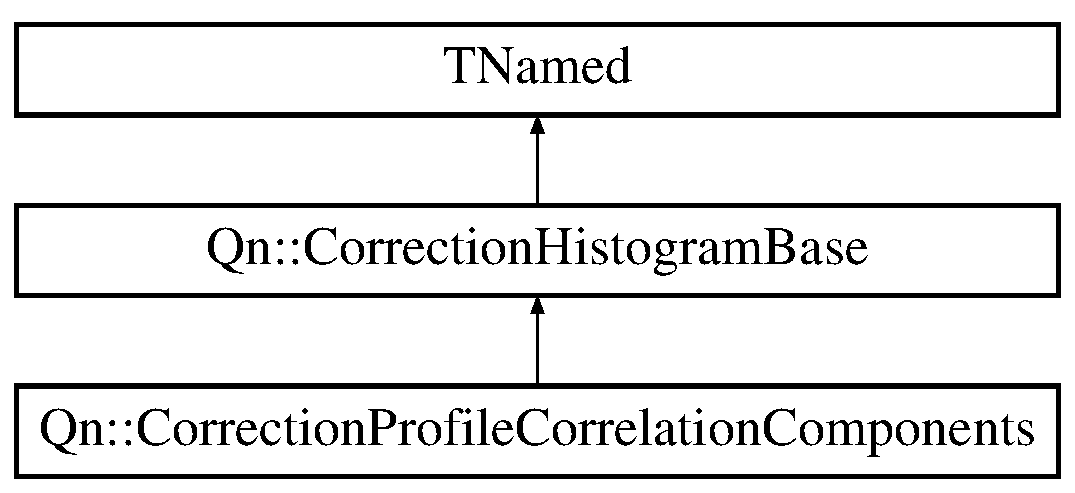
\includegraphics[height=3.000000cm]{classQn_1_1CorrectionProfileCorrelationComponents}
\end{center}
\end{figure}
\subsection*{Public Member Functions}
\begin{DoxyCompactItemize}
\item 
\mbox{\Hypertarget{classQn_1_1CorrectionProfileCorrelationComponents_ab632ed867cbc51d05116486cf2bb3dd3}\label{classQn_1_1CorrectionProfileCorrelationComponents_ab632ed867cbc51d05116486cf2bb3dd3}} 
\mbox{\hyperlink{classQn_1_1CorrectionProfileCorrelationComponents_ab632ed867cbc51d05116486cf2bb3dd3}{Correction\+Profile\+Correlation\+Components}} ()
\begin{DoxyCompactList}\small\item\em Default constructor. \end{DoxyCompactList}\item 
\mbox{\hyperlink{classQn_1_1CorrectionProfileCorrelationComponents_aae547ab6d47a7008904a05045fbcd4bf}{Correction\+Profile\+Correlation\+Components}} (const char $\ast$name, const char $\ast$title, \mbox{\hyperlink{classQn_1_1EventClassVariablesSet}{Event\+Class\+Variables\+Set}} \&ecvs, Option\+\_\+t $\ast$option=\char`\"{}\char`\"{})
\item 
virtual \mbox{\hyperlink{classQn_1_1CorrectionProfileCorrelationComponents_a172ec5effe44c5e2eb40da82c8a56bb0}{$\sim$\+Correction\+Profile\+Correlation\+Components}} ()
\item 
Bool\+\_\+t \mbox{\hyperlink{classQn_1_1CorrectionProfileCorrelationComponents_ad9ec714a26cdc2c76eb5be288f6f114e}{Create\+Correlation\+Components\+Profile\+Histograms}} (T\+List $\ast$histogram\+List)
\item 
virtual Bool\+\_\+t \mbox{\hyperlink{classQn_1_1CorrectionProfileCorrelationComponents_af2faa01d08373d0cb2e5631776729989}{Attach\+Histograms}} (T\+List $\ast$histogram\+List)
\item 
\mbox{\Hypertarget{classQn_1_1CorrectionProfileCorrelationComponents_ae6724df1041ef1049e2c7649c2e58d06}\label{classQn_1_1CorrectionProfileCorrelationComponents_ae6724df1041ef1049e2c7649c2e58d06}} 
virtual Bool\+\_\+t \mbox{\hyperlink{classQn_1_1CorrectionProfileCorrelationComponents_ae6724df1041ef1049e2c7649c2e58d06}{Attach\+Histograms}} (T\+List $\ast$histogram\+List, const Bool\+\_\+t $\ast$b\+Used\+Channel, const Int\+\_\+t $\ast$n\+Channel\+Group)
\begin{DoxyCompactList}\small\item\em wrong call for this class invoke base class behavior \end{DoxyCompactList}\item 
virtual Long64\+\_\+t \mbox{\hyperlink{classQn_1_1CorrectionProfileCorrelationComponents_a0e45d5f8e12af86c557aad48e07198a4}{Get\+Bin}} (const double $\ast$variable\+Container)
\item 
\mbox{\Hypertarget{classQn_1_1CorrectionProfileCorrelationComponents_a743cd351750d847bfc638d15218cbfa8}\label{classQn_1_1CorrectionProfileCorrelationComponents_a743cd351750d847bfc638d15218cbfa8}} 
virtual Long64\+\_\+t \mbox{\hyperlink{classQn_1_1CorrectionProfileCorrelationComponents_a743cd351750d847bfc638d15218cbfa8}{Get\+Bin}} (const double $\ast$variable\+Container, Int\+\_\+t n\+Channel)
\begin{DoxyCompactList}\small\item\em wrong call for this class invoke base class behavior \end{DoxyCompactList}\item 
virtual Bool\+\_\+t \mbox{\hyperlink{classQn_1_1CorrectionProfileCorrelationComponents_a10db27a0f3bc8c52b3b188eb7395f835}{Bin\+Content\+Validated}} (Long64\+\_\+t bin)
\item 
virtual Float\+\_\+t \mbox{\hyperlink{classQn_1_1CorrectionProfileCorrelationComponents_a8bb785420ac0cb117b2af1047cb86bb2}{Get\+X\+X\+Bin\+Content}} (Long64\+\_\+t bin)
\item 
virtual Float\+\_\+t \mbox{\hyperlink{classQn_1_1CorrectionProfileCorrelationComponents_ad690503e78ddf4017cd8813bb12e8583}{Get\+X\+Y\+Bin\+Content}} (Long64\+\_\+t bin)
\item 
virtual Float\+\_\+t \mbox{\hyperlink{classQn_1_1CorrectionProfileCorrelationComponents_a5bf66dc908aa51c9b7661a69023dd946}{Get\+Y\+X\+Bin\+Content}} (Long64\+\_\+t bin)
\item 
virtual Float\+\_\+t \mbox{\hyperlink{classQn_1_1CorrectionProfileCorrelationComponents_a6af717d8880002afe43b294f1a152546}{Get\+Y\+Y\+Bin\+Content}} (Long64\+\_\+t bin)
\item 
virtual Float\+\_\+t \mbox{\hyperlink{classQn_1_1CorrectionProfileCorrelationComponents_a76bba719fcab0995255c8309dcaf6c72}{Get\+X\+X\+Bin\+Error}} (Long64\+\_\+t bin)
\item 
virtual Float\+\_\+t \mbox{\hyperlink{classQn_1_1CorrectionProfileCorrelationComponents_a58d233f34fbbf505d6abb2cf3236c60f}{Get\+X\+Y\+Bin\+Error}} (Long64\+\_\+t bin)
\item 
virtual Float\+\_\+t \mbox{\hyperlink{classQn_1_1CorrectionProfileCorrelationComponents_a91f05094196842c16be6f6fc2bb7dad8}{Get\+Y\+X\+Bin\+Error}} (Long64\+\_\+t bin)
\item 
virtual Float\+\_\+t \mbox{\hyperlink{classQn_1_1CorrectionProfileCorrelationComponents_a4952dd516dbd12a66c7a385cbc51cc6b}{Get\+Y\+Y\+Bin\+Error}} (Long64\+\_\+t bin)
\item 
virtual void \mbox{\hyperlink{classQn_1_1CorrectionProfileCorrelationComponents_adebd3ce6b05ef6c65c1288132951ba22}{Fill\+XX}} (const double $\ast$variable\+Container, Float\+\_\+t weight)
\item 
virtual void \mbox{\hyperlink{classQn_1_1CorrectionProfileCorrelationComponents_a05d2d17173f5a6aaccb4bd8cb9aece3a}{Fill\+XY}} (const double $\ast$variable\+Container, Float\+\_\+t weight)
\item 
virtual void \mbox{\hyperlink{classQn_1_1CorrectionProfileCorrelationComponents_a8c011aed3281ab3d9fd8fd83e43ad384}{Fill\+YX}} (const double $\ast$variable\+Container, Float\+\_\+t weight)
\item 
virtual void \mbox{\hyperlink{classQn_1_1CorrectionProfileCorrelationComponents_af033e682edd09ce172db1f23cf4d6865}{Fill\+YY}} (const double $\ast$variable\+Container, Float\+\_\+t weight)
\item 
\mbox{\Hypertarget{classQn_1_1CorrectionProfileCorrelationComponents_a7db7b8e5a7a11b91de593ed60c9ed84a}\label{classQn_1_1CorrectionProfileCorrelationComponents_a7db7b8e5a7a11b91de593ed60c9ed84a}} 
virtual Float\+\_\+t \mbox{\hyperlink{classQn_1_1CorrectionProfileCorrelationComponents_a7db7b8e5a7a11b91de593ed60c9ed84a}{Get\+X\+X\+Bin\+Content}} (Int\+\_\+t harmonic, Long64\+\_\+t bin)
\begin{DoxyCompactList}\small\item\em wrong call for this class invoke base class behavior \end{DoxyCompactList}\item 
\mbox{\Hypertarget{classQn_1_1CorrectionProfileCorrelationComponents_aec422c5e452b98fed97dbe57f8613314}\label{classQn_1_1CorrectionProfileCorrelationComponents_aec422c5e452b98fed97dbe57f8613314}} 
virtual Float\+\_\+t \mbox{\hyperlink{classQn_1_1CorrectionProfileCorrelationComponents_aec422c5e452b98fed97dbe57f8613314}{Get\+X\+Y\+Bin\+Content}} (Int\+\_\+t harmonic, Long64\+\_\+t bin)
\begin{DoxyCompactList}\small\item\em wrong call for this class invoke base class behavior \end{DoxyCompactList}\item 
\mbox{\Hypertarget{classQn_1_1CorrectionProfileCorrelationComponents_a81c1b7bd19dca53c3e1e9407daffc1e6}\label{classQn_1_1CorrectionProfileCorrelationComponents_a81c1b7bd19dca53c3e1e9407daffc1e6}} 
virtual Float\+\_\+t \mbox{\hyperlink{classQn_1_1CorrectionProfileCorrelationComponents_a81c1b7bd19dca53c3e1e9407daffc1e6}{Get\+Y\+X\+Bin\+Content}} (Int\+\_\+t harmonic, Long64\+\_\+t bin)
\begin{DoxyCompactList}\small\item\em wrong call for this class invoke base class behavior \end{DoxyCompactList}\item 
\mbox{\Hypertarget{classQn_1_1CorrectionProfileCorrelationComponents_ae409fa99ff155d6a356af6f5901e2360}\label{classQn_1_1CorrectionProfileCorrelationComponents_ae409fa99ff155d6a356af6f5901e2360}} 
virtual Float\+\_\+t \mbox{\hyperlink{classQn_1_1CorrectionProfileCorrelationComponents_ae409fa99ff155d6a356af6f5901e2360}{Get\+Y\+Y\+Bin\+Content}} (Int\+\_\+t harmonic, Long64\+\_\+t bin)
\begin{DoxyCompactList}\small\item\em wrong call for this class invoke base class behavior \end{DoxyCompactList}\item 
\mbox{\Hypertarget{classQn_1_1CorrectionProfileCorrelationComponents_af27e27f474d058efe4495a90c7fa73c1}\label{classQn_1_1CorrectionProfileCorrelationComponents_af27e27f474d058efe4495a90c7fa73c1}} 
virtual Float\+\_\+t \mbox{\hyperlink{classQn_1_1CorrectionProfileCorrelationComponents_af27e27f474d058efe4495a90c7fa73c1}{Get\+X\+X\+Bin\+Error}} (Int\+\_\+t harmonic, Long64\+\_\+t bin)
\begin{DoxyCompactList}\small\item\em wrong call for this class invoke base class behavior \end{DoxyCompactList}\item 
\mbox{\Hypertarget{classQn_1_1CorrectionProfileCorrelationComponents_a1d3376133250c6af3e93441d19aebc1b}\label{classQn_1_1CorrectionProfileCorrelationComponents_a1d3376133250c6af3e93441d19aebc1b}} 
virtual Float\+\_\+t \mbox{\hyperlink{classQn_1_1CorrectionProfileCorrelationComponents_a1d3376133250c6af3e93441d19aebc1b}{Get\+X\+Y\+Bin\+Error}} (Int\+\_\+t harmonic, Long64\+\_\+t bin)
\begin{DoxyCompactList}\small\item\em wrong call for this class invoke base class behavior \end{DoxyCompactList}\item 
\mbox{\Hypertarget{classQn_1_1CorrectionProfileCorrelationComponents_aa5af19d9bf922e6be18b0f5a651a8c45}\label{classQn_1_1CorrectionProfileCorrelationComponents_aa5af19d9bf922e6be18b0f5a651a8c45}} 
virtual Float\+\_\+t \mbox{\hyperlink{classQn_1_1CorrectionProfileCorrelationComponents_aa5af19d9bf922e6be18b0f5a651a8c45}{Get\+Y\+X\+Bin\+Error}} (Int\+\_\+t harmonic, Long64\+\_\+t bin)
\begin{DoxyCompactList}\small\item\em wrong call for this class invoke base class behavior \end{DoxyCompactList}\item 
\mbox{\Hypertarget{classQn_1_1CorrectionProfileCorrelationComponents_a652f4c83e72679161bd7ea35e84a6229}\label{classQn_1_1CorrectionProfileCorrelationComponents_a652f4c83e72679161bd7ea35e84a6229}} 
virtual Float\+\_\+t \mbox{\hyperlink{classQn_1_1CorrectionProfileCorrelationComponents_a652f4c83e72679161bd7ea35e84a6229}{Get\+Y\+Y\+Bin\+Error}} (Int\+\_\+t harmonic, Long64\+\_\+t bin)
\begin{DoxyCompactList}\small\item\em wrong call for this class invoke base class behavior \end{DoxyCompactList}\item 
\mbox{\Hypertarget{classQn_1_1CorrectionProfileCorrelationComponents_a352ac53b7545ddbf21af77fb52f1581e}\label{classQn_1_1CorrectionProfileCorrelationComponents_a352ac53b7545ddbf21af77fb52f1581e}} 
virtual void \mbox{\hyperlink{classQn_1_1CorrectionProfileCorrelationComponents_a352ac53b7545ddbf21af77fb52f1581e}{Fill\+XX}} (Int\+\_\+t harmonic, const double $\ast$variable\+Container, Float\+\_\+t weight)
\begin{DoxyCompactList}\small\item\em wrong call for this class invoke base class behavior \end{DoxyCompactList}\item 
\mbox{\Hypertarget{classQn_1_1CorrectionProfileCorrelationComponents_a19373de52bf2370215a6b6e9a34c042a}\label{classQn_1_1CorrectionProfileCorrelationComponents_a19373de52bf2370215a6b6e9a34c042a}} 
virtual void \mbox{\hyperlink{classQn_1_1CorrectionProfileCorrelationComponents_a19373de52bf2370215a6b6e9a34c042a}{Fill\+XY}} (Int\+\_\+t harmonic, const double $\ast$variable\+Container, Float\+\_\+t weight)
\begin{DoxyCompactList}\small\item\em wrong call for this class invoke base class behavior \end{DoxyCompactList}\item 
\mbox{\Hypertarget{classQn_1_1CorrectionProfileCorrelationComponents_a0404a6067482047e3be1a92dbf475cd6}\label{classQn_1_1CorrectionProfileCorrelationComponents_a0404a6067482047e3be1a92dbf475cd6}} 
virtual void \mbox{\hyperlink{classQn_1_1CorrectionProfileCorrelationComponents_a0404a6067482047e3be1a92dbf475cd6}{Fill\+YX}} (Int\+\_\+t harmonic, const double $\ast$variable\+Container, Float\+\_\+t weight)
\begin{DoxyCompactList}\small\item\em wrong call for this class invoke base class behavior \end{DoxyCompactList}\item 
\mbox{\Hypertarget{classQn_1_1CorrectionProfileCorrelationComponents_a9897eecbae360761526ed3f99919df47}\label{classQn_1_1CorrectionProfileCorrelationComponents_a9897eecbae360761526ed3f99919df47}} 
virtual void \mbox{\hyperlink{classQn_1_1CorrectionProfileCorrelationComponents_a9897eecbae360761526ed3f99919df47}{Fill\+YY}} (Int\+\_\+t harmonic, const double $\ast$variable\+Container, Float\+\_\+t weight)
\begin{DoxyCompactList}\small\item\em wrong call for this class invoke base class behavior \end{DoxyCompactList}\end{DoxyCompactItemize}
\subsection*{Additional Inherited Members}


\subsection{Constructor \& Destructor Documentation}
\mbox{\Hypertarget{classQn_1_1CorrectionProfileCorrelationComponents_aae547ab6d47a7008904a05045fbcd4bf}\label{classQn_1_1CorrectionProfileCorrelationComponents_aae547ab6d47a7008904a05045fbcd4bf}} 
\index{Qn\+::\+Correction\+Profile\+Correlation\+Components@{Qn\+::\+Correction\+Profile\+Correlation\+Components}!Correction\+Profile\+Correlation\+Components@{Correction\+Profile\+Correlation\+Components}}
\index{Correction\+Profile\+Correlation\+Components@{Correction\+Profile\+Correlation\+Components}!Qn\+::\+Correction\+Profile\+Correlation\+Components@{Qn\+::\+Correction\+Profile\+Correlation\+Components}}
\subsubsection{\texorpdfstring{Correction\+Profile\+Correlation\+Components()}{CorrectionProfileCorrelationComponents()}}
{\footnotesize\ttfamily Qn\+::\+Correction\+Profile\+Correlation\+Components\+::\+Correction\+Profile\+Correlation\+Components (\begin{DoxyParamCaption}\item[{const char $\ast$}]{name,  }\item[{const char $\ast$}]{title,  }\item[{\mbox{\hyperlink{classQn_1_1EventClassVariablesSet}{Event\+Class\+Variables\+Set}} \&}]{ecvs,  }\item[{Option\+\_\+t $\ast$}]{option = {\ttfamily \char`\"{}\char`\"{}} }\end{DoxyParamCaption})}

Normal constructor

Stores the set of variables that identify the different event classes passing them to its parent and prepares the object for actual histogram creation or attachment


\begin{DoxyParams}{Parameters}
{\em name} & base for the name of the histograms \\
\hline
{\em title} & base for the title of the histograms \\
\hline
{\em ecvs} & the event classes variables set \\
\hline
{\em option} & option for errors computation \textquotesingle{} \textquotesingle{} (Default) the bin errors are the standard error on the mean of the bin values\\
\hline
\end{DoxyParams}
\textquotesingle{}s\textquotesingle{} the bin are the standard deviation of of the bin values \mbox{\Hypertarget{classQn_1_1CorrectionProfileCorrelationComponents_a172ec5effe44c5e2eb40da82c8a56bb0}\label{classQn_1_1CorrectionProfileCorrelationComponents_a172ec5effe44c5e2eb40da82c8a56bb0}} 
\index{Qn\+::\+Correction\+Profile\+Correlation\+Components@{Qn\+::\+Correction\+Profile\+Correlation\+Components}!````~Correction\+Profile\+Correlation\+Components@{$\sim$\+Correction\+Profile\+Correlation\+Components}}
\index{````~Correction\+Profile\+Correlation\+Components@{$\sim$\+Correction\+Profile\+Correlation\+Components}!Qn\+::\+Correction\+Profile\+Correlation\+Components@{Qn\+::\+Correction\+Profile\+Correlation\+Components}}
\subsubsection{\texorpdfstring{$\sim$\+Correction\+Profile\+Correlation\+Components()}{~CorrectionProfileCorrelationComponents()}}
{\footnotesize\ttfamily Qn\+::\+Correction\+Profile\+Correlation\+Components\+::$\sim$\+Correction\+Profile\+Correlation\+Components (\begin{DoxyParamCaption}{ }\end{DoxyParamCaption})\hspace{0.3cm}{\ttfamily [virtual]}}

Default destructor

Returns the only taken memory, the harmonic histograms storage, the own histograms and other members are not own at destruction time 

\subsection{Member Function Documentation}
\mbox{\Hypertarget{classQn_1_1CorrectionProfileCorrelationComponents_af2faa01d08373d0cb2e5631776729989}\label{classQn_1_1CorrectionProfileCorrelationComponents_af2faa01d08373d0cb2e5631776729989}} 
\index{Qn\+::\+Correction\+Profile\+Correlation\+Components@{Qn\+::\+Correction\+Profile\+Correlation\+Components}!Attach\+Histograms@{Attach\+Histograms}}
\index{Attach\+Histograms@{Attach\+Histograms}!Qn\+::\+Correction\+Profile\+Correlation\+Components@{Qn\+::\+Correction\+Profile\+Correlation\+Components}}
\subsubsection{\texorpdfstring{Attach\+Histograms()}{AttachHistograms()}}
{\footnotesize\ttfamily Bool\+\_\+t Qn\+::\+Correction\+Profile\+Correlation\+Components\+::\+Attach\+Histograms (\begin{DoxyParamCaption}\item[{T\+List $\ast$}]{histogram\+List }\end{DoxyParamCaption})\hspace{0.3cm}{\ttfamily [virtual]}}

Attaches existing histograms as the support histograms for XX, XY, YX, YY correlation component of the profile function for different harmonics

The histograms are located in the passed list and if found and with the proper dimensions their references are stored in member variables.

The harmonic map is inferred from the found histograms within the list that match the naming scheme.


\begin{DoxyParams}{Parameters}
{\em histogram\+List} & list where the histograms have to be located \\
\hline
\end{DoxyParams}
\begin{DoxyReturn}{Returns}
true if properly attached else false 
\end{DoxyReturn}


Reimplemented from \mbox{\hyperlink{classQn_1_1CorrectionHistogramBase_ad8bcd0079fe5db561780a522e46b7b16}{Qn\+::\+Correction\+Histogram\+Base}}.

\mbox{\Hypertarget{classQn_1_1CorrectionProfileCorrelationComponents_a10db27a0f3bc8c52b3b188eb7395f835}\label{classQn_1_1CorrectionProfileCorrelationComponents_a10db27a0f3bc8c52b3b188eb7395f835}} 
\index{Qn\+::\+Correction\+Profile\+Correlation\+Components@{Qn\+::\+Correction\+Profile\+Correlation\+Components}!Bin\+Content\+Validated@{Bin\+Content\+Validated}}
\index{Bin\+Content\+Validated@{Bin\+Content\+Validated}!Qn\+::\+Correction\+Profile\+Correlation\+Components@{Qn\+::\+Correction\+Profile\+Correlation\+Components}}
\subsubsection{\texorpdfstring{Bin\+Content\+Validated()}{BinContentValidated()}}
{\footnotesize\ttfamily Bool\+\_\+t Qn\+::\+Correction\+Profile\+Correlation\+Components\+::\+Bin\+Content\+Validated (\begin{DoxyParamCaption}\item[{Long64\+\_\+t}]{bin }\end{DoxyParamCaption})\hspace{0.3cm}{\ttfamily [virtual]}}

Check the validity of the content of the passed bin If the number of entries is lower than the minimum number of entries to validate it the bin content is not considered valid and k\+F\+A\+L\+SE is returned, otherwise k\+T\+R\+UE is returned 
\begin{DoxyParams}{Parameters}
{\em bin} & the bin to check its content validity \\
\hline
\end{DoxyParams}
\begin{DoxyReturn}{Returns}
k\+T\+R\+UE if the content is valid k\+F\+A\+L\+SE otherwise 
\end{DoxyReturn}


Implements \mbox{\hyperlink{classQn_1_1CorrectionHistogramBase_a4db2c92ceaffefaa91475a721612d80d}{Qn\+::\+Correction\+Histogram\+Base}}.

\mbox{\Hypertarget{classQn_1_1CorrectionProfileCorrelationComponents_ad9ec714a26cdc2c76eb5be288f6f114e}\label{classQn_1_1CorrectionProfileCorrelationComponents_ad9ec714a26cdc2c76eb5be288f6f114e}} 
\index{Qn\+::\+Correction\+Profile\+Correlation\+Components@{Qn\+::\+Correction\+Profile\+Correlation\+Components}!Create\+Correlation\+Components\+Profile\+Histograms@{Create\+Correlation\+Components\+Profile\+Histograms}}
\index{Create\+Correlation\+Components\+Profile\+Histograms@{Create\+Correlation\+Components\+Profile\+Histograms}!Qn\+::\+Correction\+Profile\+Correlation\+Components@{Qn\+::\+Correction\+Profile\+Correlation\+Components}}
\subsubsection{\texorpdfstring{Create\+Correlation\+Components\+Profile\+Histograms()}{CreateCorrelationComponentsProfileHistograms()}}
{\footnotesize\ttfamily Bool\+\_\+t Qn\+::\+Correction\+Profile\+Correlation\+Components\+::\+Create\+Correlation\+Components\+Profile\+Histograms (\begin{DoxyParamCaption}\item[{T\+List $\ast$}]{histogram\+List }\end{DoxyParamCaption})}

Creates the XX, XY, YX, YY correlation components support histograms for the profile function

Based in the event classes variables set in the parent class the values and entries multidimensional histograms are created.

Four values histograms are created, XX,XY, YX and YY. The fully filled condition is computed and stored

The whole set of histograms are added to the passed histogram list


\begin{DoxyParams}{Parameters}
{\em histogram\+List} & list where the histograms have to be added \\
\hline
\end{DoxyParams}
\begin{DoxyReturn}{Returns}
true if properly created 
\end{DoxyReturn}
\mbox{\Hypertarget{classQn_1_1CorrectionProfileCorrelationComponents_adebd3ce6b05ef6c65c1288132951ba22}\label{classQn_1_1CorrectionProfileCorrelationComponents_adebd3ce6b05ef6c65c1288132951ba22}} 
\index{Qn\+::\+Correction\+Profile\+Correlation\+Components@{Qn\+::\+Correction\+Profile\+Correlation\+Components}!Fill\+XX@{Fill\+XX}}
\index{Fill\+XX@{Fill\+XX}!Qn\+::\+Correction\+Profile\+Correlation\+Components@{Qn\+::\+Correction\+Profile\+Correlation\+Components}}
\subsubsection{\texorpdfstring{Fill\+X\+X()}{FillXX()}}
{\footnotesize\ttfamily void Qn\+::\+Correction\+Profile\+Correlation\+Components\+::\+Fill\+XX (\begin{DoxyParamCaption}\item[{const double $\ast$}]{variable\+Container,  }\item[{Float\+\_\+t}]{weight }\end{DoxyParamCaption})\hspace{0.3cm}{\ttfamily [virtual]}}

Fills the XX correlation component.

The involved bin is computed according to the current variables content. The bin is then increased by the given weight. The entries count is only updated if the whole set for the four components has been already filled. A check is done for detecting consecutive fills without a previous entries update.


\begin{DoxyParams}{Parameters}
{\em variable\+Container} & the current variables content addressed by var Id \\
\hline
{\em weight} & the increment in the bin content \\
\hline
\end{DoxyParams}


Reimplemented from \mbox{\hyperlink{classQn_1_1CorrectionHistogramBase_a42a813abe035719dddedf2102fbfbdc9}{Qn\+::\+Correction\+Histogram\+Base}}.

\mbox{\Hypertarget{classQn_1_1CorrectionProfileCorrelationComponents_a05d2d17173f5a6aaccb4bd8cb9aece3a}\label{classQn_1_1CorrectionProfileCorrelationComponents_a05d2d17173f5a6aaccb4bd8cb9aece3a}} 
\index{Qn\+::\+Correction\+Profile\+Correlation\+Components@{Qn\+::\+Correction\+Profile\+Correlation\+Components}!Fill\+XY@{Fill\+XY}}
\index{Fill\+XY@{Fill\+XY}!Qn\+::\+Correction\+Profile\+Correlation\+Components@{Qn\+::\+Correction\+Profile\+Correlation\+Components}}
\subsubsection{\texorpdfstring{Fill\+X\+Y()}{FillXY()}}
{\footnotesize\ttfamily void Qn\+::\+Correction\+Profile\+Correlation\+Components\+::\+Fill\+XY (\begin{DoxyParamCaption}\item[{const double $\ast$}]{variable\+Container,  }\item[{Float\+\_\+t}]{weight }\end{DoxyParamCaption})\hspace{0.3cm}{\ttfamily [virtual]}}

Fills the XY correlation component.

The involved bin is computed according to the current variables content. The bin is then increased by the given weight. The entries count is only updated if the whole set for the four components has been already filled. A check is done for detecting consecutive fills without a previous entries update.


\begin{DoxyParams}{Parameters}
{\em variable\+Container} & the current variables content addressed by var Id \\
\hline
{\em weight} & the increment in the bin content \\
\hline
\end{DoxyParams}


Reimplemented from \mbox{\hyperlink{classQn_1_1CorrectionHistogramBase_a3ede7e510526e205704ec78e7c7254a3}{Qn\+::\+Correction\+Histogram\+Base}}.

\mbox{\Hypertarget{classQn_1_1CorrectionProfileCorrelationComponents_a8c011aed3281ab3d9fd8fd83e43ad384}\label{classQn_1_1CorrectionProfileCorrelationComponents_a8c011aed3281ab3d9fd8fd83e43ad384}} 
\index{Qn\+::\+Correction\+Profile\+Correlation\+Components@{Qn\+::\+Correction\+Profile\+Correlation\+Components}!Fill\+YX@{Fill\+YX}}
\index{Fill\+YX@{Fill\+YX}!Qn\+::\+Correction\+Profile\+Correlation\+Components@{Qn\+::\+Correction\+Profile\+Correlation\+Components}}
\subsubsection{\texorpdfstring{Fill\+Y\+X()}{FillYX()}}
{\footnotesize\ttfamily void Qn\+::\+Correction\+Profile\+Correlation\+Components\+::\+Fill\+YX (\begin{DoxyParamCaption}\item[{const double $\ast$}]{variable\+Container,  }\item[{Float\+\_\+t}]{weight }\end{DoxyParamCaption})\hspace{0.3cm}{\ttfamily [virtual]}}

Fills the YX correlation component.

The involved bin is computed according to the current variables content. The bin is then increased by the given weight. The entries count is only updated if the whole set for the four components has been already filled. A check is done for detecting consecutive fills without a previous entries update.


\begin{DoxyParams}{Parameters}
{\em variable\+Container} & the current variables content addressed by var Id \\
\hline
{\em weight} & the increment in the bin content \\
\hline
\end{DoxyParams}


Reimplemented from \mbox{\hyperlink{classQn_1_1CorrectionHistogramBase_a70d3afc8ffdca9af505143d365c210bc}{Qn\+::\+Correction\+Histogram\+Base}}.

\mbox{\Hypertarget{classQn_1_1CorrectionProfileCorrelationComponents_af033e682edd09ce172db1f23cf4d6865}\label{classQn_1_1CorrectionProfileCorrelationComponents_af033e682edd09ce172db1f23cf4d6865}} 
\index{Qn\+::\+Correction\+Profile\+Correlation\+Components@{Qn\+::\+Correction\+Profile\+Correlation\+Components}!Fill\+YY@{Fill\+YY}}
\index{Fill\+YY@{Fill\+YY}!Qn\+::\+Correction\+Profile\+Correlation\+Components@{Qn\+::\+Correction\+Profile\+Correlation\+Components}}
\subsubsection{\texorpdfstring{Fill\+Y\+Y()}{FillYY()}}
{\footnotesize\ttfamily void Qn\+::\+Correction\+Profile\+Correlation\+Components\+::\+Fill\+YY (\begin{DoxyParamCaption}\item[{const double $\ast$}]{variable\+Container,  }\item[{Float\+\_\+t}]{weight }\end{DoxyParamCaption})\hspace{0.3cm}{\ttfamily [virtual]}}

Fills the YY correlation component.

The involved bin is computed according to the current variables content. The bin is then increased by the given weight. The entries count is only updated if the whole set for the four components has been already filled. A check is done for detecting consecutive fills without a previous entries update.


\begin{DoxyParams}{Parameters}
{\em variable\+Container} & the current variables content addressed by var Id \\
\hline
{\em weight} & the increment in the bin content \\
\hline
\end{DoxyParams}


Reimplemented from \mbox{\hyperlink{classQn_1_1CorrectionHistogramBase_a06e19e77ff3ba40039b3e1d84ad7a227}{Qn\+::\+Correction\+Histogram\+Base}}.

\mbox{\Hypertarget{classQn_1_1CorrectionProfileCorrelationComponents_a0e45d5f8e12af86c557aad48e07198a4}\label{classQn_1_1CorrectionProfileCorrelationComponents_a0e45d5f8e12af86c557aad48e07198a4}} 
\index{Qn\+::\+Correction\+Profile\+Correlation\+Components@{Qn\+::\+Correction\+Profile\+Correlation\+Components}!Get\+Bin@{Get\+Bin}}
\index{Get\+Bin@{Get\+Bin}!Qn\+::\+Correction\+Profile\+Correlation\+Components@{Qn\+::\+Correction\+Profile\+Correlation\+Components}}
\subsubsection{\texorpdfstring{Get\+Bin()}{GetBin()}}
{\footnotesize\ttfamily Long64\+\_\+t Qn\+::\+Correction\+Profile\+Correlation\+Components\+::\+Get\+Bin (\begin{DoxyParamCaption}\item[{const double $\ast$}]{variable\+Container }\end{DoxyParamCaption})\hspace{0.3cm}{\ttfamily [virtual]}}

Get the bin number for the current variable content

The bin number identifies the event class the current variable content points to.


\begin{DoxyParams}{Parameters}
{\em variable\+Container} & the current variables content addressed by var Id \\
\hline
\end{DoxyParams}
\begin{DoxyReturn}{Returns}
the associated bin to the current variables content 
\end{DoxyReturn}


Reimplemented from \mbox{\hyperlink{classQn_1_1CorrectionHistogramBase_ab1f64550f4e1812864da6f9f6ea565e6}{Qn\+::\+Correction\+Histogram\+Base}}.

\mbox{\Hypertarget{classQn_1_1CorrectionProfileCorrelationComponents_a8bb785420ac0cb117b2af1047cb86bb2}\label{classQn_1_1CorrectionProfileCorrelationComponents_a8bb785420ac0cb117b2af1047cb86bb2}} 
\index{Qn\+::\+Correction\+Profile\+Correlation\+Components@{Qn\+::\+Correction\+Profile\+Correlation\+Components}!Get\+X\+X\+Bin\+Content@{Get\+X\+X\+Bin\+Content}}
\index{Get\+X\+X\+Bin\+Content@{Get\+X\+X\+Bin\+Content}!Qn\+::\+Correction\+Profile\+Correlation\+Components@{Qn\+::\+Correction\+Profile\+Correlation\+Components}}
\subsubsection{\texorpdfstring{Get\+X\+X\+Bin\+Content()}{GetXXBinContent()}}
{\footnotesize\ttfamily Float\+\_\+t Qn\+::\+Correction\+Profile\+Correlation\+Components\+::\+Get\+X\+X\+Bin\+Content (\begin{DoxyParamCaption}\item[{Long64\+\_\+t}]{bin }\end{DoxyParamCaption})\hspace{0.3cm}{\ttfamily [virtual]}}

Get the XX correlation component bin content.

The bin number identifies a desired event class whose content is requested. If the bin is not validated zero is returned.


\begin{DoxyParams}{Parameters}
{\em bin} & the interested bin number \\
\hline
\end{DoxyParams}
\begin{DoxyReturn}{Returns}
the bin number content 
\end{DoxyReturn}


Reimplemented from \mbox{\hyperlink{classQn_1_1CorrectionHistogramBase_a5ed53d98b57fa9e9ec4de78ae518d9d9}{Qn\+::\+Correction\+Histogram\+Base}}.

\mbox{\Hypertarget{classQn_1_1CorrectionProfileCorrelationComponents_a76bba719fcab0995255c8309dcaf6c72}\label{classQn_1_1CorrectionProfileCorrelationComponents_a76bba719fcab0995255c8309dcaf6c72}} 
\index{Qn\+::\+Correction\+Profile\+Correlation\+Components@{Qn\+::\+Correction\+Profile\+Correlation\+Components}!Get\+X\+X\+Bin\+Error@{Get\+X\+X\+Bin\+Error}}
\index{Get\+X\+X\+Bin\+Error@{Get\+X\+X\+Bin\+Error}!Qn\+::\+Correction\+Profile\+Correlation\+Components@{Qn\+::\+Correction\+Profile\+Correlation\+Components}}
\subsubsection{\texorpdfstring{Get\+X\+X\+Bin\+Error()}{GetXXBinError()}}
{\footnotesize\ttfamily Float\+\_\+t Qn\+::\+Correction\+Profile\+Correlation\+Components\+::\+Get\+X\+X\+Bin\+Error (\begin{DoxyParamCaption}\item[{Long64\+\_\+t}]{bin }\end{DoxyParamCaption})\hspace{0.3cm}{\ttfamily [virtual]}}

Get the XX correlation component bin content error for the passed bin number.

The bin number identifies a desired event class whose content is error is requested. If the bin is not validated zero is returned.


\begin{DoxyParams}{Parameters}
{\em bin} & the interested bin number \\
\hline
\end{DoxyParams}
\begin{DoxyReturn}{Returns}
the bin content error 
\end{DoxyReturn}


Reimplemented from \mbox{\hyperlink{classQn_1_1CorrectionHistogramBase_ae7b4e0bfb45e52cc7050eefc78c5230e}{Qn\+::\+Correction\+Histogram\+Base}}.

\mbox{\Hypertarget{classQn_1_1CorrectionProfileCorrelationComponents_ad690503e78ddf4017cd8813bb12e8583}\label{classQn_1_1CorrectionProfileCorrelationComponents_ad690503e78ddf4017cd8813bb12e8583}} 
\index{Qn\+::\+Correction\+Profile\+Correlation\+Components@{Qn\+::\+Correction\+Profile\+Correlation\+Components}!Get\+X\+Y\+Bin\+Content@{Get\+X\+Y\+Bin\+Content}}
\index{Get\+X\+Y\+Bin\+Content@{Get\+X\+Y\+Bin\+Content}!Qn\+::\+Correction\+Profile\+Correlation\+Components@{Qn\+::\+Correction\+Profile\+Correlation\+Components}}
\subsubsection{\texorpdfstring{Get\+X\+Y\+Bin\+Content()}{GetXYBinContent()}}
{\footnotesize\ttfamily Float\+\_\+t Qn\+::\+Correction\+Profile\+Correlation\+Components\+::\+Get\+X\+Y\+Bin\+Content (\begin{DoxyParamCaption}\item[{Long64\+\_\+t}]{bin }\end{DoxyParamCaption})\hspace{0.3cm}{\ttfamily [virtual]}}

Get the XY correlation component bin content.

The bin number identifies a desired event class whose content is requested. If the bin is not validated zero is returned.


\begin{DoxyParams}{Parameters}
{\em bin} & the interested bin number \\
\hline
\end{DoxyParams}
\begin{DoxyReturn}{Returns}
the bin number content 
\end{DoxyReturn}


Reimplemented from \mbox{\hyperlink{classQn_1_1CorrectionHistogramBase_aa631b6234a81dbe46b29a95fda339b69}{Qn\+::\+Correction\+Histogram\+Base}}.

\mbox{\Hypertarget{classQn_1_1CorrectionProfileCorrelationComponents_a58d233f34fbbf505d6abb2cf3236c60f}\label{classQn_1_1CorrectionProfileCorrelationComponents_a58d233f34fbbf505d6abb2cf3236c60f}} 
\index{Qn\+::\+Correction\+Profile\+Correlation\+Components@{Qn\+::\+Correction\+Profile\+Correlation\+Components}!Get\+X\+Y\+Bin\+Error@{Get\+X\+Y\+Bin\+Error}}
\index{Get\+X\+Y\+Bin\+Error@{Get\+X\+Y\+Bin\+Error}!Qn\+::\+Correction\+Profile\+Correlation\+Components@{Qn\+::\+Correction\+Profile\+Correlation\+Components}}
\subsubsection{\texorpdfstring{Get\+X\+Y\+Bin\+Error()}{GetXYBinError()}}
{\footnotesize\ttfamily Float\+\_\+t Qn\+::\+Correction\+Profile\+Correlation\+Components\+::\+Get\+X\+Y\+Bin\+Error (\begin{DoxyParamCaption}\item[{Long64\+\_\+t}]{bin }\end{DoxyParamCaption})\hspace{0.3cm}{\ttfamily [virtual]}}

Get the XY correlation component bin content error for the passed bin number.

The bin number identifies a desired event class whose content is error is requested. If the bin is not validated zero is returned.


\begin{DoxyParams}{Parameters}
{\em bin} & the interested bin number \\
\hline
\end{DoxyParams}
\begin{DoxyReturn}{Returns}
the bin content error 
\end{DoxyReturn}


Reimplemented from \mbox{\hyperlink{classQn_1_1CorrectionHistogramBase_ae7dada656dda33ba9adca7bcbd78f4d2}{Qn\+::\+Correction\+Histogram\+Base}}.

\mbox{\Hypertarget{classQn_1_1CorrectionProfileCorrelationComponents_a5bf66dc908aa51c9b7661a69023dd946}\label{classQn_1_1CorrectionProfileCorrelationComponents_a5bf66dc908aa51c9b7661a69023dd946}} 
\index{Qn\+::\+Correction\+Profile\+Correlation\+Components@{Qn\+::\+Correction\+Profile\+Correlation\+Components}!Get\+Y\+X\+Bin\+Content@{Get\+Y\+X\+Bin\+Content}}
\index{Get\+Y\+X\+Bin\+Content@{Get\+Y\+X\+Bin\+Content}!Qn\+::\+Correction\+Profile\+Correlation\+Components@{Qn\+::\+Correction\+Profile\+Correlation\+Components}}
\subsubsection{\texorpdfstring{Get\+Y\+X\+Bin\+Content()}{GetYXBinContent()}}
{\footnotesize\ttfamily Float\+\_\+t Qn\+::\+Correction\+Profile\+Correlation\+Components\+::\+Get\+Y\+X\+Bin\+Content (\begin{DoxyParamCaption}\item[{Long64\+\_\+t}]{bin }\end{DoxyParamCaption})\hspace{0.3cm}{\ttfamily [virtual]}}

Get the YX correlation component bin content.

The bin number identifies a desired event class whose content is requested. If the bin is not validated zero is returned.


\begin{DoxyParams}{Parameters}
{\em bin} & the interested bin number \\
\hline
\end{DoxyParams}
\begin{DoxyReturn}{Returns}
the bin number content 
\end{DoxyReturn}


Reimplemented from \mbox{\hyperlink{classQn_1_1CorrectionHistogramBase_a2bc9c26889a5ff0479f5638e2e253174}{Qn\+::\+Correction\+Histogram\+Base}}.

\mbox{\Hypertarget{classQn_1_1CorrectionProfileCorrelationComponents_a91f05094196842c16be6f6fc2bb7dad8}\label{classQn_1_1CorrectionProfileCorrelationComponents_a91f05094196842c16be6f6fc2bb7dad8}} 
\index{Qn\+::\+Correction\+Profile\+Correlation\+Components@{Qn\+::\+Correction\+Profile\+Correlation\+Components}!Get\+Y\+X\+Bin\+Error@{Get\+Y\+X\+Bin\+Error}}
\index{Get\+Y\+X\+Bin\+Error@{Get\+Y\+X\+Bin\+Error}!Qn\+::\+Correction\+Profile\+Correlation\+Components@{Qn\+::\+Correction\+Profile\+Correlation\+Components}}
\subsubsection{\texorpdfstring{Get\+Y\+X\+Bin\+Error()}{GetYXBinError()}}
{\footnotesize\ttfamily Float\+\_\+t Qn\+::\+Correction\+Profile\+Correlation\+Components\+::\+Get\+Y\+X\+Bin\+Error (\begin{DoxyParamCaption}\item[{Long64\+\_\+t}]{bin }\end{DoxyParamCaption})\hspace{0.3cm}{\ttfamily [virtual]}}

Get the YX correlation component bin content error for the passed bin number.

The bin number identifies a desired event class whose content is error is requested. If the bin is not validated zero is returned.


\begin{DoxyParams}{Parameters}
{\em bin} & the interested bin number \\
\hline
\end{DoxyParams}
\begin{DoxyReturn}{Returns}
the bin content error 
\end{DoxyReturn}


Reimplemented from \mbox{\hyperlink{classQn_1_1CorrectionHistogramBase_a07055fbf2b7df0ee3912fd68c18572c0}{Qn\+::\+Correction\+Histogram\+Base}}.

\mbox{\Hypertarget{classQn_1_1CorrectionProfileCorrelationComponents_a6af717d8880002afe43b294f1a152546}\label{classQn_1_1CorrectionProfileCorrelationComponents_a6af717d8880002afe43b294f1a152546}} 
\index{Qn\+::\+Correction\+Profile\+Correlation\+Components@{Qn\+::\+Correction\+Profile\+Correlation\+Components}!Get\+Y\+Y\+Bin\+Content@{Get\+Y\+Y\+Bin\+Content}}
\index{Get\+Y\+Y\+Bin\+Content@{Get\+Y\+Y\+Bin\+Content}!Qn\+::\+Correction\+Profile\+Correlation\+Components@{Qn\+::\+Correction\+Profile\+Correlation\+Components}}
\subsubsection{\texorpdfstring{Get\+Y\+Y\+Bin\+Content()}{GetYYBinContent()}}
{\footnotesize\ttfamily Float\+\_\+t Qn\+::\+Correction\+Profile\+Correlation\+Components\+::\+Get\+Y\+Y\+Bin\+Content (\begin{DoxyParamCaption}\item[{Long64\+\_\+t}]{bin }\end{DoxyParamCaption})\hspace{0.3cm}{\ttfamily [virtual]}}

Get the YY correlation component bin content.

The bin number identifies a desired event class whose content is requested. If the bin is not validated zero is returned.


\begin{DoxyParams}{Parameters}
{\em bin} & the interested bin number \\
\hline
\end{DoxyParams}
\begin{DoxyReturn}{Returns}
the bin number content 
\end{DoxyReturn}


Reimplemented from \mbox{\hyperlink{classQn_1_1CorrectionHistogramBase_a1ebb8ccb23cce80b276670617f4c03e5}{Qn\+::\+Correction\+Histogram\+Base}}.

\mbox{\Hypertarget{classQn_1_1CorrectionProfileCorrelationComponents_a4952dd516dbd12a66c7a385cbc51cc6b}\label{classQn_1_1CorrectionProfileCorrelationComponents_a4952dd516dbd12a66c7a385cbc51cc6b}} 
\index{Qn\+::\+Correction\+Profile\+Correlation\+Components@{Qn\+::\+Correction\+Profile\+Correlation\+Components}!Get\+Y\+Y\+Bin\+Error@{Get\+Y\+Y\+Bin\+Error}}
\index{Get\+Y\+Y\+Bin\+Error@{Get\+Y\+Y\+Bin\+Error}!Qn\+::\+Correction\+Profile\+Correlation\+Components@{Qn\+::\+Correction\+Profile\+Correlation\+Components}}
\subsubsection{\texorpdfstring{Get\+Y\+Y\+Bin\+Error()}{GetYYBinError()}}
{\footnotesize\ttfamily Float\+\_\+t Qn\+::\+Correction\+Profile\+Correlation\+Components\+::\+Get\+Y\+Y\+Bin\+Error (\begin{DoxyParamCaption}\item[{Long64\+\_\+t}]{bin }\end{DoxyParamCaption})\hspace{0.3cm}{\ttfamily [virtual]}}

Get the YY correlation component bin content error for the passed bin number.

The bin number identifies a desired event class whose content is error is requested. If the bin is not validated zero is returned.


\begin{DoxyParams}{Parameters}
{\em bin} & the interested bin number \\
\hline
\end{DoxyParams}
\begin{DoxyReturn}{Returns}
the bin content error 
\end{DoxyReturn}


Reimplemented from \mbox{\hyperlink{classQn_1_1CorrectionHistogramBase_aec361c84c8291093f17ae6839384eeb9}{Qn\+::\+Correction\+Histogram\+Base}}.



The documentation for this class was generated from the following files\+:\begin{DoxyCompactItemize}
\item 
D\+T\+\_\+\+Flow/\+Qn\+Corrections/include/Correction\+Profile\+Correlation\+Components.\+h\item 
D\+T\+\_\+\+Flow/\+Qn\+Corrections/Correction\+Profile\+Correlation\+Components.\+cpp\end{DoxyCompactItemize}

\hypertarget{classQn_1_1CorrectionProfileCorrelationComponentsHarmonics}{}\section{Qn\+:\+:Correction\+Profile\+Correlation\+Components\+Harmonics Class Reference}
\label{classQn_1_1CorrectionProfileCorrelationComponentsHarmonics}\index{Qn\+::\+Correction\+Profile\+Correlation\+Components\+Harmonics@{Qn\+::\+Correction\+Profile\+Correlation\+Components\+Harmonics}}
Inheritance diagram for Qn\+:\+:Correction\+Profile\+Correlation\+Components\+Harmonics\+:\begin{figure}[H]
\begin{center}
\leavevmode
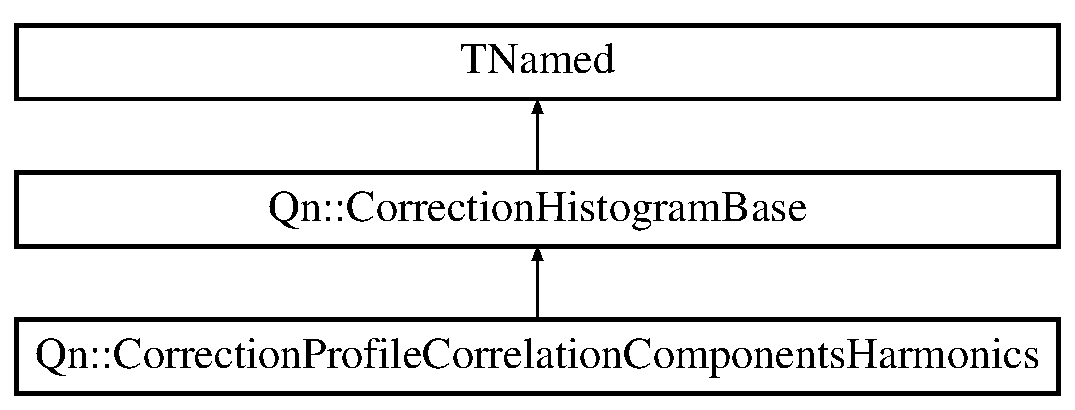
\includegraphics[height=3.000000cm]{classQn_1_1CorrectionProfileCorrelationComponentsHarmonics}
\end{center}
\end{figure}
\subsection*{Public Member Functions}
\begin{DoxyCompactItemize}
\item 
\mbox{\Hypertarget{classQn_1_1CorrectionProfileCorrelationComponentsHarmonics_a4fbf93f74a23339984288928e4a916dc}\label{classQn_1_1CorrectionProfileCorrelationComponentsHarmonics_a4fbf93f74a23339984288928e4a916dc}} 
\mbox{\hyperlink{classQn_1_1CorrectionProfileCorrelationComponentsHarmonics_a4fbf93f74a23339984288928e4a916dc}{Correction\+Profile\+Correlation\+Components\+Harmonics}} ()
\begin{DoxyCompactList}\small\item\em Default constructor. \end{DoxyCompactList}\item 
\mbox{\hyperlink{classQn_1_1CorrectionProfileCorrelationComponentsHarmonics_a87efcaa6fb3a2e3bf1296bafc977aa3d}{Correction\+Profile\+Correlation\+Components\+Harmonics}} (const char $\ast$name, const char $\ast$title, \mbox{\hyperlink{classQn_1_1EventClassVariablesSet}{Event\+Class\+Variables\+Set}} \&ecvs, Option\+\_\+t $\ast$option=\char`\"{}\char`\"{})
\item 
virtual \mbox{\hyperlink{classQn_1_1CorrectionProfileCorrelationComponentsHarmonics_a68cad43115b31ed195d3553a7fa1dd52}{$\sim$\+Correction\+Profile\+Correlation\+Components\+Harmonics}} ()
\item 
Bool\+\_\+t \mbox{\hyperlink{classQn_1_1CorrectionProfileCorrelationComponentsHarmonics_a397aabf8866ef1056d04198a55a9d660}{Create\+Correlation\+Components\+Profile\+Histograms}} (T\+List $\ast$histogram\+List, Int\+\_\+t n\+No\+Of\+Harmonics, Int\+\_\+t $\ast$harmonic\+Map=N\+U\+LL)
\item 
virtual Bool\+\_\+t \mbox{\hyperlink{classQn_1_1CorrectionProfileCorrelationComponentsHarmonics_ab338a5263d8eb124c3a6a0bbde5f72e3}{Attach\+Histograms}} (T\+List $\ast$histogram\+List)
\item 
\mbox{\Hypertarget{classQn_1_1CorrectionProfileCorrelationComponentsHarmonics_a2e4534d5d49ec13573619dd48735b044}\label{classQn_1_1CorrectionProfileCorrelationComponentsHarmonics_a2e4534d5d49ec13573619dd48735b044}} 
virtual Bool\+\_\+t \mbox{\hyperlink{classQn_1_1CorrectionProfileCorrelationComponentsHarmonics_a2e4534d5d49ec13573619dd48735b044}{Attach\+Histograms}} (T\+List $\ast$histogram\+List, const Bool\+\_\+t $\ast$b\+Used\+Channel, const Int\+\_\+t $\ast$n\+Channel\+Group)
\begin{DoxyCompactList}\small\item\em wrong call for this class invoke base class behavior \end{DoxyCompactList}\item 
virtual Long64\+\_\+t \mbox{\hyperlink{classQn_1_1CorrectionProfileCorrelationComponentsHarmonics_a51113d377e95ddd78f89adb9c2cd52df}{Get\+Bin}} (const double $\ast$variable\+Container)
\item 
\mbox{\Hypertarget{classQn_1_1CorrectionProfileCorrelationComponentsHarmonics_af500f2c1e6751686dfb060c268e9cef5}\label{classQn_1_1CorrectionProfileCorrelationComponentsHarmonics_af500f2c1e6751686dfb060c268e9cef5}} 
virtual Long64\+\_\+t \mbox{\hyperlink{classQn_1_1CorrectionProfileCorrelationComponentsHarmonics_af500f2c1e6751686dfb060c268e9cef5}{Get\+Bin}} (const double $\ast$variable\+Container, Int\+\_\+t n\+Channel)
\begin{DoxyCompactList}\small\item\em wrong call for this class invoke base class behavior \end{DoxyCompactList}\item 
virtual Bool\+\_\+t \mbox{\hyperlink{classQn_1_1CorrectionProfileCorrelationComponentsHarmonics_aed95bd8eea2e060ba3040d25f3533177}{Bin\+Content\+Validated}} (Long64\+\_\+t bin)
\item 
virtual Float\+\_\+t \mbox{\hyperlink{classQn_1_1CorrectionProfileCorrelationComponentsHarmonics_aa48fa859f512dcd7b7e0a7c7ede4bb99}{Get\+X\+X\+Bin\+Content}} (Int\+\_\+t harmonic, Long64\+\_\+t bin)
\item 
virtual Float\+\_\+t \mbox{\hyperlink{classQn_1_1CorrectionProfileCorrelationComponentsHarmonics_af7d5feb2bafb19417950f6d16cdfceb0}{Get\+X\+Y\+Bin\+Content}} (Int\+\_\+t harmonic, Long64\+\_\+t bin)
\item 
virtual Float\+\_\+t \mbox{\hyperlink{classQn_1_1CorrectionProfileCorrelationComponentsHarmonics_a14b776082f56bec058ef29e6ae69fed1}{Get\+Y\+X\+Bin\+Content}} (Int\+\_\+t harmonic, Long64\+\_\+t bin)
\item 
virtual Float\+\_\+t \mbox{\hyperlink{classQn_1_1CorrectionProfileCorrelationComponentsHarmonics_a0256be6f18beb3a2562891e2912b55fb}{Get\+Y\+Y\+Bin\+Content}} (Int\+\_\+t harmonic, Long64\+\_\+t bin)
\item 
virtual Float\+\_\+t \mbox{\hyperlink{classQn_1_1CorrectionProfileCorrelationComponentsHarmonics_a412fe35fd2adf2a73a6ddfdad4a3f880}{Get\+X\+X\+Bin\+Error}} (Int\+\_\+t harmonic, Long64\+\_\+t bin)
\item 
virtual Float\+\_\+t \mbox{\hyperlink{classQn_1_1CorrectionProfileCorrelationComponentsHarmonics_ac3aada46be56f35fa487ed621889b121}{Get\+X\+Y\+Bin\+Error}} (Int\+\_\+t harmonic, Long64\+\_\+t bin)
\item 
virtual Float\+\_\+t \mbox{\hyperlink{classQn_1_1CorrectionProfileCorrelationComponentsHarmonics_a27ddadf86598339c7cc6bbdc8f5475fe}{Get\+Y\+X\+Bin\+Error}} (Int\+\_\+t harmonic, Long64\+\_\+t bin)
\item 
virtual Float\+\_\+t \mbox{\hyperlink{classQn_1_1CorrectionProfileCorrelationComponentsHarmonics_a66b580c99a004f475f612b0835ff9da1}{Get\+Y\+Y\+Bin\+Error}} (Int\+\_\+t harmonic, Long64\+\_\+t bin)
\item 
virtual void \mbox{\hyperlink{classQn_1_1CorrectionProfileCorrelationComponentsHarmonics_a6f62753a3c19725bca87c408b4ba62a9}{Fill\+XX}} (Int\+\_\+t harmonic, const double $\ast$variable\+Container, Float\+\_\+t weight)
\item 
virtual void \mbox{\hyperlink{classQn_1_1CorrectionProfileCorrelationComponentsHarmonics_a2ab0d7bd1188858fb1953812d2732e7e}{Fill\+XY}} (Int\+\_\+t harmonic, const double $\ast$variable\+Container, Float\+\_\+t weight)
\item 
virtual void \mbox{\hyperlink{classQn_1_1CorrectionProfileCorrelationComponentsHarmonics_a233a81523a12204f57104edcacd0bf31}{Fill\+YX}} (Int\+\_\+t harmonic, const double $\ast$variable\+Container, Float\+\_\+t weight)
\item 
virtual void \mbox{\hyperlink{classQn_1_1CorrectionProfileCorrelationComponentsHarmonics_a3bb3424e5ff93d56e925f0b60a57a90c}{Fill\+YY}} (Int\+\_\+t harmonic, const double $\ast$variable\+Container, Float\+\_\+t weight)
\item 
\mbox{\Hypertarget{classQn_1_1CorrectionProfileCorrelationComponentsHarmonics_a4002be74c4146565fa0f93789b739463}\label{classQn_1_1CorrectionProfileCorrelationComponentsHarmonics_a4002be74c4146565fa0f93789b739463}} 
virtual Float\+\_\+t \mbox{\hyperlink{classQn_1_1CorrectionProfileCorrelationComponentsHarmonics_a4002be74c4146565fa0f93789b739463}{Get\+X\+X\+Bin\+Content}} (Long64\+\_\+t bin)
\begin{DoxyCompactList}\small\item\em wrong call for this class invoke base class behavior \end{DoxyCompactList}\item 
\mbox{\Hypertarget{classQn_1_1CorrectionProfileCorrelationComponentsHarmonics_a41d1dce57a2eab50abf2a02aaf7cce1e}\label{classQn_1_1CorrectionProfileCorrelationComponentsHarmonics_a41d1dce57a2eab50abf2a02aaf7cce1e}} 
virtual Float\+\_\+t \mbox{\hyperlink{classQn_1_1CorrectionProfileCorrelationComponentsHarmonics_a41d1dce57a2eab50abf2a02aaf7cce1e}{Get\+X\+Y\+Bin\+Content}} (Long64\+\_\+t bin)
\begin{DoxyCompactList}\small\item\em wrong call for this class invoke base class behavior \end{DoxyCompactList}\item 
\mbox{\Hypertarget{classQn_1_1CorrectionProfileCorrelationComponentsHarmonics_a5cad74c0b9396b104ab630c246bf19df}\label{classQn_1_1CorrectionProfileCorrelationComponentsHarmonics_a5cad74c0b9396b104ab630c246bf19df}} 
virtual Float\+\_\+t \mbox{\hyperlink{classQn_1_1CorrectionProfileCorrelationComponentsHarmonics_a5cad74c0b9396b104ab630c246bf19df}{Get\+Y\+X\+Bin\+Content}} (Long64\+\_\+t bin)
\begin{DoxyCompactList}\small\item\em wrong call for this class invoke base class behavior \end{DoxyCompactList}\item 
\mbox{\Hypertarget{classQn_1_1CorrectionProfileCorrelationComponentsHarmonics_a17da16c438a33b56f2bb6ecdbca36ca7}\label{classQn_1_1CorrectionProfileCorrelationComponentsHarmonics_a17da16c438a33b56f2bb6ecdbca36ca7}} 
virtual Float\+\_\+t \mbox{\hyperlink{classQn_1_1CorrectionProfileCorrelationComponentsHarmonics_a17da16c438a33b56f2bb6ecdbca36ca7}{Get\+Y\+Y\+Bin\+Content}} (Long64\+\_\+t bin)
\begin{DoxyCompactList}\small\item\em wrong call for this class invoke base class behavior \end{DoxyCompactList}\item 
\mbox{\Hypertarget{classQn_1_1CorrectionProfileCorrelationComponentsHarmonics_a492f84a9286ac565f42933d1630b1e0e}\label{classQn_1_1CorrectionProfileCorrelationComponentsHarmonics_a492f84a9286ac565f42933d1630b1e0e}} 
virtual Float\+\_\+t \mbox{\hyperlink{classQn_1_1CorrectionProfileCorrelationComponentsHarmonics_a492f84a9286ac565f42933d1630b1e0e}{Get\+X\+X\+Bin\+Error}} (Long64\+\_\+t bin)
\begin{DoxyCompactList}\small\item\em wrong call for this class invoke base class behavior \end{DoxyCompactList}\item 
\mbox{\Hypertarget{classQn_1_1CorrectionProfileCorrelationComponentsHarmonics_a4dbf495bfa861a2cf2a59182271c43a9}\label{classQn_1_1CorrectionProfileCorrelationComponentsHarmonics_a4dbf495bfa861a2cf2a59182271c43a9}} 
virtual Float\+\_\+t \mbox{\hyperlink{classQn_1_1CorrectionProfileCorrelationComponentsHarmonics_a4dbf495bfa861a2cf2a59182271c43a9}{Get\+X\+Y\+Bin\+Error}} (Long64\+\_\+t bin)
\begin{DoxyCompactList}\small\item\em wrong call for this class invoke base class behavior \end{DoxyCompactList}\item 
\mbox{\Hypertarget{classQn_1_1CorrectionProfileCorrelationComponentsHarmonics_a2fb45faa92d49c538af35235ced49240}\label{classQn_1_1CorrectionProfileCorrelationComponentsHarmonics_a2fb45faa92d49c538af35235ced49240}} 
virtual Float\+\_\+t \mbox{\hyperlink{classQn_1_1CorrectionProfileCorrelationComponentsHarmonics_a2fb45faa92d49c538af35235ced49240}{Get\+Y\+X\+Bin\+Error}} (Long64\+\_\+t bin)
\begin{DoxyCompactList}\small\item\em wrong call for this class invoke base class behavior \end{DoxyCompactList}\item 
\mbox{\Hypertarget{classQn_1_1CorrectionProfileCorrelationComponentsHarmonics_a2c790c78673796616e18bc1f793a6f1e}\label{classQn_1_1CorrectionProfileCorrelationComponentsHarmonics_a2c790c78673796616e18bc1f793a6f1e}} 
virtual Float\+\_\+t \mbox{\hyperlink{classQn_1_1CorrectionProfileCorrelationComponentsHarmonics_a2c790c78673796616e18bc1f793a6f1e}{Get\+Y\+Y\+Bin\+Error}} (Long64\+\_\+t bin)
\begin{DoxyCompactList}\small\item\em wrong call for this class invoke base class behavior \end{DoxyCompactList}\item 
\mbox{\Hypertarget{classQn_1_1CorrectionProfileCorrelationComponentsHarmonics_a631174884439d99dee2d04678d1e64aa}\label{classQn_1_1CorrectionProfileCorrelationComponentsHarmonics_a631174884439d99dee2d04678d1e64aa}} 
virtual void \mbox{\hyperlink{classQn_1_1CorrectionProfileCorrelationComponentsHarmonics_a631174884439d99dee2d04678d1e64aa}{Fill\+XX}} (const double $\ast$variable\+Container, Float\+\_\+t weight)
\begin{DoxyCompactList}\small\item\em wrong call for this class invoke base class behavior \end{DoxyCompactList}\item 
\mbox{\Hypertarget{classQn_1_1CorrectionProfileCorrelationComponentsHarmonics_a59fc7f772621466f60cbf34a98c0174c}\label{classQn_1_1CorrectionProfileCorrelationComponentsHarmonics_a59fc7f772621466f60cbf34a98c0174c}} 
virtual void \mbox{\hyperlink{classQn_1_1CorrectionProfileCorrelationComponentsHarmonics_a59fc7f772621466f60cbf34a98c0174c}{Fill\+XY}} (const double $\ast$variable\+Container, Float\+\_\+t weight)
\begin{DoxyCompactList}\small\item\em wrong call for this class invoke base class behavior \end{DoxyCompactList}\item 
\mbox{\Hypertarget{classQn_1_1CorrectionProfileCorrelationComponentsHarmonics_a04d5ba4313e4ebab81ffe203970c8cf3}\label{classQn_1_1CorrectionProfileCorrelationComponentsHarmonics_a04d5ba4313e4ebab81ffe203970c8cf3}} 
virtual void \mbox{\hyperlink{classQn_1_1CorrectionProfileCorrelationComponentsHarmonics_a04d5ba4313e4ebab81ffe203970c8cf3}{Fill\+YX}} (const double $\ast$variable\+Container, Float\+\_\+t weight)
\begin{DoxyCompactList}\small\item\em wrong call for this class invoke base class behavior \end{DoxyCompactList}\item 
\mbox{\Hypertarget{classQn_1_1CorrectionProfileCorrelationComponentsHarmonics_a2616f4bc573bb7d8cd3ff69d7f0b5e12}\label{classQn_1_1CorrectionProfileCorrelationComponentsHarmonics_a2616f4bc573bb7d8cd3ff69d7f0b5e12}} 
virtual void \mbox{\hyperlink{classQn_1_1CorrectionProfileCorrelationComponentsHarmonics_a2616f4bc573bb7d8cd3ff69d7f0b5e12}{Fill\+YY}} (const double $\ast$variable\+Container, Float\+\_\+t weight)
\begin{DoxyCompactList}\small\item\em wrong call for this class invoke base class behavior \end{DoxyCompactList}\end{DoxyCompactItemize}
\subsection*{Additional Inherited Members}


\subsection{Constructor \& Destructor Documentation}
\mbox{\Hypertarget{classQn_1_1CorrectionProfileCorrelationComponentsHarmonics_a87efcaa6fb3a2e3bf1296bafc977aa3d}\label{classQn_1_1CorrectionProfileCorrelationComponentsHarmonics_a87efcaa6fb3a2e3bf1296bafc977aa3d}} 
\index{Qn\+::\+Correction\+Profile\+Correlation\+Components\+Harmonics@{Qn\+::\+Correction\+Profile\+Correlation\+Components\+Harmonics}!Correction\+Profile\+Correlation\+Components\+Harmonics@{Correction\+Profile\+Correlation\+Components\+Harmonics}}
\index{Correction\+Profile\+Correlation\+Components\+Harmonics@{Correction\+Profile\+Correlation\+Components\+Harmonics}!Qn\+::\+Correction\+Profile\+Correlation\+Components\+Harmonics@{Qn\+::\+Correction\+Profile\+Correlation\+Components\+Harmonics}}
\subsubsection{\texorpdfstring{Correction\+Profile\+Correlation\+Components\+Harmonics()}{CorrectionProfileCorrelationComponentsHarmonics()}}
{\footnotesize\ttfamily Qn\+::\+Correction\+Profile\+Correlation\+Components\+Harmonics\+::\+Correction\+Profile\+Correlation\+Components\+Harmonics (\begin{DoxyParamCaption}\item[{const char $\ast$}]{name,  }\item[{const char $\ast$}]{title,  }\item[{\mbox{\hyperlink{classQn_1_1EventClassVariablesSet}{Event\+Class\+Variables\+Set}} \&}]{ecvs,  }\item[{Option\+\_\+t $\ast$}]{option = {\ttfamily \char`\"{}\char`\"{}} }\end{DoxyParamCaption})}

Normal constructor

Stores the set of variables that identify the different event classes passing them to its parent and prepares the object for actual histogram creation or attachment


\begin{DoxyParams}{Parameters}
{\em name} & base for the name of the histograms \\
\hline
{\em title} & base for the title of the histograms \\
\hline
{\em ecvs} & the event classes variables set \\
\hline
{\em option} & option for errors computation \textquotesingle{} \textquotesingle{} (Default) the bin errors are the standard error on the mean of the bin values\\
\hline
\end{DoxyParams}
\textquotesingle{}s\textquotesingle{} the bin are the standard deviation of of the bin values \mbox{\Hypertarget{classQn_1_1CorrectionProfileCorrelationComponentsHarmonics_a68cad43115b31ed195d3553a7fa1dd52}\label{classQn_1_1CorrectionProfileCorrelationComponentsHarmonics_a68cad43115b31ed195d3553a7fa1dd52}} 
\index{Qn\+::\+Correction\+Profile\+Correlation\+Components\+Harmonics@{Qn\+::\+Correction\+Profile\+Correlation\+Components\+Harmonics}!````~Correction\+Profile\+Correlation\+Components\+Harmonics@{$\sim$\+Correction\+Profile\+Correlation\+Components\+Harmonics}}
\index{````~Correction\+Profile\+Correlation\+Components\+Harmonics@{$\sim$\+Correction\+Profile\+Correlation\+Components\+Harmonics}!Qn\+::\+Correction\+Profile\+Correlation\+Components\+Harmonics@{Qn\+::\+Correction\+Profile\+Correlation\+Components\+Harmonics}}
\subsubsection{\texorpdfstring{$\sim$\+Correction\+Profile\+Correlation\+Components\+Harmonics()}{~CorrectionProfileCorrelationComponentsHarmonics()}}
{\footnotesize\ttfamily Qn\+::\+Correction\+Profile\+Correlation\+Components\+Harmonics\+::$\sim$\+Correction\+Profile\+Correlation\+Components\+Harmonics (\begin{DoxyParamCaption}{ }\end{DoxyParamCaption})\hspace{0.3cm}{\ttfamily [virtual]}}

Default destructor

Returns the only taken memory, the harmonic histograms storage, the own histograms and other members are not own at destruction time 

\subsection{Member Function Documentation}
\mbox{\Hypertarget{classQn_1_1CorrectionProfileCorrelationComponentsHarmonics_ab338a5263d8eb124c3a6a0bbde5f72e3}\label{classQn_1_1CorrectionProfileCorrelationComponentsHarmonics_ab338a5263d8eb124c3a6a0bbde5f72e3}} 
\index{Qn\+::\+Correction\+Profile\+Correlation\+Components\+Harmonics@{Qn\+::\+Correction\+Profile\+Correlation\+Components\+Harmonics}!Attach\+Histograms@{Attach\+Histograms}}
\index{Attach\+Histograms@{Attach\+Histograms}!Qn\+::\+Correction\+Profile\+Correlation\+Components\+Harmonics@{Qn\+::\+Correction\+Profile\+Correlation\+Components\+Harmonics}}
\subsubsection{\texorpdfstring{Attach\+Histograms()}{AttachHistograms()}}
{\footnotesize\ttfamily Bool\+\_\+t Qn\+::\+Correction\+Profile\+Correlation\+Components\+Harmonics\+::\+Attach\+Histograms (\begin{DoxyParamCaption}\item[{T\+List $\ast$}]{histogram\+List }\end{DoxyParamCaption})\hspace{0.3cm}{\ttfamily [virtual]}}

Attaches existing histograms as the support histograms for XX, XY, YX, YY correlation component of the profile function for different harmonics

The histograms are located in the passed list and if found and with the proper dimensions their references are stored in member variables.

The harmonic map is inferred from the found histograms within the list that match the naming scheme.


\begin{DoxyParams}{Parameters}
{\em histogram\+List} & list where the histograms have to be located \\
\hline
\end{DoxyParams}
\begin{DoxyReturn}{Returns}
true if properly attached else false 
\end{DoxyReturn}


Reimplemented from \mbox{\hyperlink{classQn_1_1CorrectionHistogramBase_ad8bcd0079fe5db561780a522e46b7b16}{Qn\+::\+Correction\+Histogram\+Base}}.

\mbox{\Hypertarget{classQn_1_1CorrectionProfileCorrelationComponentsHarmonics_aed95bd8eea2e060ba3040d25f3533177}\label{classQn_1_1CorrectionProfileCorrelationComponentsHarmonics_aed95bd8eea2e060ba3040d25f3533177}} 
\index{Qn\+::\+Correction\+Profile\+Correlation\+Components\+Harmonics@{Qn\+::\+Correction\+Profile\+Correlation\+Components\+Harmonics}!Bin\+Content\+Validated@{Bin\+Content\+Validated}}
\index{Bin\+Content\+Validated@{Bin\+Content\+Validated}!Qn\+::\+Correction\+Profile\+Correlation\+Components\+Harmonics@{Qn\+::\+Correction\+Profile\+Correlation\+Components\+Harmonics}}
\subsubsection{\texorpdfstring{Bin\+Content\+Validated()}{BinContentValidated()}}
{\footnotesize\ttfamily Bool\+\_\+t Qn\+::\+Correction\+Profile\+Correlation\+Components\+Harmonics\+::\+Bin\+Content\+Validated (\begin{DoxyParamCaption}\item[{Long64\+\_\+t}]{bin }\end{DoxyParamCaption})\hspace{0.3cm}{\ttfamily [virtual]}}

Check the validity of the content of the passed bin If the number of entries is lower than the minimum number of entries to validate it the bin content is not considered valid and k\+F\+A\+L\+SE is returned, otherwise k\+T\+R\+UE is returned 
\begin{DoxyParams}{Parameters}
{\em bin} & the bin to check its content validity \\
\hline
\end{DoxyParams}
\begin{DoxyReturn}{Returns}
k\+T\+R\+UE if the content is valid k\+F\+A\+L\+SE otherwise 
\end{DoxyReturn}


Implements \mbox{\hyperlink{classQn_1_1CorrectionHistogramBase_a4db2c92ceaffefaa91475a721612d80d}{Qn\+::\+Correction\+Histogram\+Base}}.

\mbox{\Hypertarget{classQn_1_1CorrectionProfileCorrelationComponentsHarmonics_a397aabf8866ef1056d04198a55a9d660}\label{classQn_1_1CorrectionProfileCorrelationComponentsHarmonics_a397aabf8866ef1056d04198a55a9d660}} 
\index{Qn\+::\+Correction\+Profile\+Correlation\+Components\+Harmonics@{Qn\+::\+Correction\+Profile\+Correlation\+Components\+Harmonics}!Create\+Correlation\+Components\+Profile\+Histograms@{Create\+Correlation\+Components\+Profile\+Histograms}}
\index{Create\+Correlation\+Components\+Profile\+Histograms@{Create\+Correlation\+Components\+Profile\+Histograms}!Qn\+::\+Correction\+Profile\+Correlation\+Components\+Harmonics@{Qn\+::\+Correction\+Profile\+Correlation\+Components\+Harmonics}}
\subsubsection{\texorpdfstring{Create\+Correlation\+Components\+Profile\+Histograms()}{CreateCorrelationComponentsProfileHistograms()}}
{\footnotesize\ttfamily Bool\+\_\+t Qn\+::\+Correction\+Profile\+Correlation\+Components\+Harmonics\+::\+Create\+Correlation\+Components\+Profile\+Histograms (\begin{DoxyParamCaption}\item[{T\+List $\ast$}]{histogram\+List,  }\item[{Int\+\_\+t}]{n\+No\+Of\+Harmonics,  }\item[{Int\+\_\+t $\ast$}]{harmonic\+Map = {\ttfamily NULL} }\end{DoxyParamCaption})}

Creates the XX, XY, YX, YY correlation components support histograms for the profile function

Based in the event classes variables set in the parent class the values and entries multidimensional histograms are created.

For each harmonic number fout values histograms are created, XX, XY, YX and YY. The histograms are organized to support external harmonic number. By default the external harmonic number is always considered to start by one. If no map is passed as parameter the external harmonic numbers are considered as\+: 1, 2, ..., n\+No\+Of\+Harmonic. If the user wants a different assignment he has to provide an ordered map, for instance\+: four harmonics with external harmonic numbers 2, 4, 6 and 8 will require n\+No\+Of\+Harmonics = 4 and harmonic\+Map = \mbox{[}2, 4, 6, 8\mbox{]}. The fully filled condition is computed and stored

The whole set of histograms are added to the passed histogram list


\begin{DoxyParams}{Parameters}
{\em histogram\+List} & list where the histograms have to be added \\
\hline
{\em n\+No\+Of\+Harmonics} & the desired number of harmonics \\
\hline
{\em harmonic\+Map} & ordered array with the external number of the harmonics \\
\hline
\end{DoxyParams}
\begin{DoxyReturn}{Returns}
true if properly created 
\end{DoxyReturn}
\mbox{\Hypertarget{classQn_1_1CorrectionProfileCorrelationComponentsHarmonics_a6f62753a3c19725bca87c408b4ba62a9}\label{classQn_1_1CorrectionProfileCorrelationComponentsHarmonics_a6f62753a3c19725bca87c408b4ba62a9}} 
\index{Qn\+::\+Correction\+Profile\+Correlation\+Components\+Harmonics@{Qn\+::\+Correction\+Profile\+Correlation\+Components\+Harmonics}!Fill\+XX@{Fill\+XX}}
\index{Fill\+XX@{Fill\+XX}!Qn\+::\+Correction\+Profile\+Correlation\+Components\+Harmonics@{Qn\+::\+Correction\+Profile\+Correlation\+Components\+Harmonics}}
\subsubsection{\texorpdfstring{Fill\+X\+X()}{FillXX()}}
{\footnotesize\ttfamily void Qn\+::\+Correction\+Profile\+Correlation\+Components\+Harmonics\+::\+Fill\+XX (\begin{DoxyParamCaption}\item[{Int\+\_\+t}]{harmonic,  }\item[{const double $\ast$}]{variable\+Container,  }\item[{Float\+\_\+t}]{weight }\end{DoxyParamCaption})\hspace{0.3cm}{\ttfamily [virtual]}}

Fills the XX correlation component for the corresponding harmonic histogram

The involved bin is computed according to the current variables content. The bin is then increased by the given weight. The entries count is only updated if the whole set for the four components has been already filled. A check is done for detecting consecutive fills for certain harmonic without a previous entries update.


\begin{DoxyParams}{Parameters}
{\em harmonic} & the interested external harmonic number \\
\hline
{\em variable\+Container} & the current variables content addressed by var Id \\
\hline
{\em weight} & the increment in the bin content \\
\hline
\end{DoxyParams}


Reimplemented from \mbox{\hyperlink{classQn_1_1CorrectionHistogramBase_a6947a657eade839da923b156d99ca10d}{Qn\+::\+Correction\+Histogram\+Base}}.

\mbox{\Hypertarget{classQn_1_1CorrectionProfileCorrelationComponentsHarmonics_a2ab0d7bd1188858fb1953812d2732e7e}\label{classQn_1_1CorrectionProfileCorrelationComponentsHarmonics_a2ab0d7bd1188858fb1953812d2732e7e}} 
\index{Qn\+::\+Correction\+Profile\+Correlation\+Components\+Harmonics@{Qn\+::\+Correction\+Profile\+Correlation\+Components\+Harmonics}!Fill\+XY@{Fill\+XY}}
\index{Fill\+XY@{Fill\+XY}!Qn\+::\+Correction\+Profile\+Correlation\+Components\+Harmonics@{Qn\+::\+Correction\+Profile\+Correlation\+Components\+Harmonics}}
\subsubsection{\texorpdfstring{Fill\+X\+Y()}{FillXY()}}
{\footnotesize\ttfamily void Qn\+::\+Correction\+Profile\+Correlation\+Components\+Harmonics\+::\+Fill\+XY (\begin{DoxyParamCaption}\item[{Int\+\_\+t}]{harmonic,  }\item[{const double $\ast$}]{variable\+Container,  }\item[{Float\+\_\+t}]{weight }\end{DoxyParamCaption})\hspace{0.3cm}{\ttfamily [virtual]}}

Fills the XY correlation component for the corresponding harmonic histogram

The involved bin is computed according to the current variables content. The bin is then increased by the given weight. The entries count is only updated if the whole set for the four components has been already filled. A check is done for detecting consecutive fills for certain harmonic without a previous entries update.


\begin{DoxyParams}{Parameters}
{\em harmonic} & the interested external harmonic number \\
\hline
{\em variable\+Container} & the current variables content addressed by var Id \\
\hline
{\em weight} & the increment in the bin content \\
\hline
\end{DoxyParams}


Reimplemented from \mbox{\hyperlink{classQn_1_1CorrectionHistogramBase_a93a446798e53ea386ce0e3fc882abae8}{Qn\+::\+Correction\+Histogram\+Base}}.

\mbox{\Hypertarget{classQn_1_1CorrectionProfileCorrelationComponentsHarmonics_a233a81523a12204f57104edcacd0bf31}\label{classQn_1_1CorrectionProfileCorrelationComponentsHarmonics_a233a81523a12204f57104edcacd0bf31}} 
\index{Qn\+::\+Correction\+Profile\+Correlation\+Components\+Harmonics@{Qn\+::\+Correction\+Profile\+Correlation\+Components\+Harmonics}!Fill\+YX@{Fill\+YX}}
\index{Fill\+YX@{Fill\+YX}!Qn\+::\+Correction\+Profile\+Correlation\+Components\+Harmonics@{Qn\+::\+Correction\+Profile\+Correlation\+Components\+Harmonics}}
\subsubsection{\texorpdfstring{Fill\+Y\+X()}{FillYX()}}
{\footnotesize\ttfamily void Qn\+::\+Correction\+Profile\+Correlation\+Components\+Harmonics\+::\+Fill\+YX (\begin{DoxyParamCaption}\item[{Int\+\_\+t}]{harmonic,  }\item[{const double $\ast$}]{variable\+Container,  }\item[{Float\+\_\+t}]{weight }\end{DoxyParamCaption})\hspace{0.3cm}{\ttfamily [virtual]}}

Fills the YX correlation component for the corresponding harmonic histogram

The involved bin is computed according to the current variables content. The bin is then increased by the given weight. The entries count is only updated if the whole set for the four components has been already filled. A check is done for detecting consecutive fills for certain harmonic without a previous entries update.


\begin{DoxyParams}{Parameters}
{\em harmonic} & the interested external harmonic number \\
\hline
{\em variable\+Container} & the current variables content addressed by var Id \\
\hline
{\em weight} & the increment in the bin content \\
\hline
\end{DoxyParams}


Reimplemented from \mbox{\hyperlink{classQn_1_1CorrectionHistogramBase_a3acc9d80584f1909771f3fcaac98d5e4}{Qn\+::\+Correction\+Histogram\+Base}}.

\mbox{\Hypertarget{classQn_1_1CorrectionProfileCorrelationComponentsHarmonics_a3bb3424e5ff93d56e925f0b60a57a90c}\label{classQn_1_1CorrectionProfileCorrelationComponentsHarmonics_a3bb3424e5ff93d56e925f0b60a57a90c}} 
\index{Qn\+::\+Correction\+Profile\+Correlation\+Components\+Harmonics@{Qn\+::\+Correction\+Profile\+Correlation\+Components\+Harmonics}!Fill\+YY@{Fill\+YY}}
\index{Fill\+YY@{Fill\+YY}!Qn\+::\+Correction\+Profile\+Correlation\+Components\+Harmonics@{Qn\+::\+Correction\+Profile\+Correlation\+Components\+Harmonics}}
\subsubsection{\texorpdfstring{Fill\+Y\+Y()}{FillYY()}}
{\footnotesize\ttfamily void Qn\+::\+Correction\+Profile\+Correlation\+Components\+Harmonics\+::\+Fill\+YY (\begin{DoxyParamCaption}\item[{Int\+\_\+t}]{harmonic,  }\item[{const double $\ast$}]{variable\+Container,  }\item[{Float\+\_\+t}]{weight }\end{DoxyParamCaption})\hspace{0.3cm}{\ttfamily [virtual]}}

Fills the YY correlation component for the corresponding harmonic histogram

The involved bin is computed according to the current variables content. The bin is then increased by the given weight. The entries count is only updated if the whole set for the four components has been already filled. A check is done for detecting consecutive fills for certain harmonic without a previous entries update.


\begin{DoxyParams}{Parameters}
{\em harmonic} & the interested external harmonic number \\
\hline
{\em variable\+Container} & the current variables content addressed by var Id \\
\hline
{\em weight} & the increment in the bin content \\
\hline
\end{DoxyParams}


Reimplemented from \mbox{\hyperlink{classQn_1_1CorrectionHistogramBase_a47c735fa34636b5d7132fff4029f13b5}{Qn\+::\+Correction\+Histogram\+Base}}.

\mbox{\Hypertarget{classQn_1_1CorrectionProfileCorrelationComponentsHarmonics_a51113d377e95ddd78f89adb9c2cd52df}\label{classQn_1_1CorrectionProfileCorrelationComponentsHarmonics_a51113d377e95ddd78f89adb9c2cd52df}} 
\index{Qn\+::\+Correction\+Profile\+Correlation\+Components\+Harmonics@{Qn\+::\+Correction\+Profile\+Correlation\+Components\+Harmonics}!Get\+Bin@{Get\+Bin}}
\index{Get\+Bin@{Get\+Bin}!Qn\+::\+Correction\+Profile\+Correlation\+Components\+Harmonics@{Qn\+::\+Correction\+Profile\+Correlation\+Components\+Harmonics}}
\subsubsection{\texorpdfstring{Get\+Bin()}{GetBin()}}
{\footnotesize\ttfamily Long64\+\_\+t Qn\+::\+Correction\+Profile\+Correlation\+Components\+Harmonics\+::\+Get\+Bin (\begin{DoxyParamCaption}\item[{const double $\ast$}]{variable\+Container }\end{DoxyParamCaption})\hspace{0.3cm}{\ttfamily [virtual]}}

Get the bin number for the current variable content

The bin number identifies the event class the current variable content points to.


\begin{DoxyParams}{Parameters}
{\em variable\+Container} & the current variables content addressed by var Id \\
\hline
\end{DoxyParams}
\begin{DoxyReturn}{Returns}
the associated bin to the current variables content 
\end{DoxyReturn}


Reimplemented from \mbox{\hyperlink{classQn_1_1CorrectionHistogramBase_ab1f64550f4e1812864da6f9f6ea565e6}{Qn\+::\+Correction\+Histogram\+Base}}.

\mbox{\Hypertarget{classQn_1_1CorrectionProfileCorrelationComponentsHarmonics_aa48fa859f512dcd7b7e0a7c7ede4bb99}\label{classQn_1_1CorrectionProfileCorrelationComponentsHarmonics_aa48fa859f512dcd7b7e0a7c7ede4bb99}} 
\index{Qn\+::\+Correction\+Profile\+Correlation\+Components\+Harmonics@{Qn\+::\+Correction\+Profile\+Correlation\+Components\+Harmonics}!Get\+X\+X\+Bin\+Content@{Get\+X\+X\+Bin\+Content}}
\index{Get\+X\+X\+Bin\+Content@{Get\+X\+X\+Bin\+Content}!Qn\+::\+Correction\+Profile\+Correlation\+Components\+Harmonics@{Qn\+::\+Correction\+Profile\+Correlation\+Components\+Harmonics}}
\subsubsection{\texorpdfstring{Get\+X\+X\+Bin\+Content()}{GetXXBinContent()}}
{\footnotesize\ttfamily Float\+\_\+t Qn\+::\+Correction\+Profile\+Correlation\+Components\+Harmonics\+::\+Get\+X\+X\+Bin\+Content (\begin{DoxyParamCaption}\item[{Int\+\_\+t}]{harmonic,  }\item[{Long64\+\_\+t}]{bin }\end{DoxyParamCaption})\hspace{0.3cm}{\ttfamily [virtual]}}

Get the XX correlation component bin content for the passed bin number for the corresponding harmonic

The bin number identifies a desired event class whose content is requested. If the bin content is not validated zero is returned.


\begin{DoxyParams}{Parameters}
{\em harmonic} & the interested external harmonic number \\
\hline
{\em bin} & the interested bin number \\
\hline
\end{DoxyParams}
\begin{DoxyReturn}{Returns}
the bin number content 
\end{DoxyReturn}


Reimplemented from \mbox{\hyperlink{classQn_1_1CorrectionHistogramBase_ac28c760f664f1b52fb6bef3f85f7ce94}{Qn\+::\+Correction\+Histogram\+Base}}.

\mbox{\Hypertarget{classQn_1_1CorrectionProfileCorrelationComponentsHarmonics_a412fe35fd2adf2a73a6ddfdad4a3f880}\label{classQn_1_1CorrectionProfileCorrelationComponentsHarmonics_a412fe35fd2adf2a73a6ddfdad4a3f880}} 
\index{Qn\+::\+Correction\+Profile\+Correlation\+Components\+Harmonics@{Qn\+::\+Correction\+Profile\+Correlation\+Components\+Harmonics}!Get\+X\+X\+Bin\+Error@{Get\+X\+X\+Bin\+Error}}
\index{Get\+X\+X\+Bin\+Error@{Get\+X\+X\+Bin\+Error}!Qn\+::\+Correction\+Profile\+Correlation\+Components\+Harmonics@{Qn\+::\+Correction\+Profile\+Correlation\+Components\+Harmonics}}
\subsubsection{\texorpdfstring{Get\+X\+X\+Bin\+Error()}{GetXXBinError()}}
{\footnotesize\ttfamily Float\+\_\+t Qn\+::\+Correction\+Profile\+Correlation\+Components\+Harmonics\+::\+Get\+X\+X\+Bin\+Error (\begin{DoxyParamCaption}\item[{Int\+\_\+t}]{harmonic,  }\item[{Long64\+\_\+t}]{bin }\end{DoxyParamCaption})\hspace{0.3cm}{\ttfamily [virtual]}}

Get the XX correlation component bin content error for the passed bin number for the corresponding harmonic

The bin number identifies a desired event class whose content is error is requested. If the bin content is not validated zero is returned.


\begin{DoxyParams}{Parameters}
{\em harmonic} & the interested external harmonic number \\
\hline
{\em bin} & the interested bin number \\
\hline
\end{DoxyParams}
\begin{DoxyReturn}{Returns}
the bin content error 
\end{DoxyReturn}


Reimplemented from \mbox{\hyperlink{classQn_1_1CorrectionHistogramBase_a6c0874928f737e86a7f72cba9a9922b7}{Qn\+::\+Correction\+Histogram\+Base}}.

\mbox{\Hypertarget{classQn_1_1CorrectionProfileCorrelationComponentsHarmonics_af7d5feb2bafb19417950f6d16cdfceb0}\label{classQn_1_1CorrectionProfileCorrelationComponentsHarmonics_af7d5feb2bafb19417950f6d16cdfceb0}} 
\index{Qn\+::\+Correction\+Profile\+Correlation\+Components\+Harmonics@{Qn\+::\+Correction\+Profile\+Correlation\+Components\+Harmonics}!Get\+X\+Y\+Bin\+Content@{Get\+X\+Y\+Bin\+Content}}
\index{Get\+X\+Y\+Bin\+Content@{Get\+X\+Y\+Bin\+Content}!Qn\+::\+Correction\+Profile\+Correlation\+Components\+Harmonics@{Qn\+::\+Correction\+Profile\+Correlation\+Components\+Harmonics}}
\subsubsection{\texorpdfstring{Get\+X\+Y\+Bin\+Content()}{GetXYBinContent()}}
{\footnotesize\ttfamily Float\+\_\+t Qn\+::\+Correction\+Profile\+Correlation\+Components\+Harmonics\+::\+Get\+X\+Y\+Bin\+Content (\begin{DoxyParamCaption}\item[{Int\+\_\+t}]{harmonic,  }\item[{Long64\+\_\+t}]{bin }\end{DoxyParamCaption})\hspace{0.3cm}{\ttfamily [virtual]}}

Get the XY correlation component bin content for the passed bin number for the corresponding harmonic

The bin number identifies a desired event class whose content is requested. If the bin content is not validated zero is returned.


\begin{DoxyParams}{Parameters}
{\em harmonic} & the interested external harmonic number \\
\hline
{\em bin} & the interested bin number \\
\hline
\end{DoxyParams}
\begin{DoxyReturn}{Returns}
the bin number content 
\end{DoxyReturn}


Reimplemented from \mbox{\hyperlink{classQn_1_1CorrectionHistogramBase_a88e6cd702547df1b8ea0fcc371dc090d}{Qn\+::\+Correction\+Histogram\+Base}}.

\mbox{\Hypertarget{classQn_1_1CorrectionProfileCorrelationComponentsHarmonics_ac3aada46be56f35fa487ed621889b121}\label{classQn_1_1CorrectionProfileCorrelationComponentsHarmonics_ac3aada46be56f35fa487ed621889b121}} 
\index{Qn\+::\+Correction\+Profile\+Correlation\+Components\+Harmonics@{Qn\+::\+Correction\+Profile\+Correlation\+Components\+Harmonics}!Get\+X\+Y\+Bin\+Error@{Get\+X\+Y\+Bin\+Error}}
\index{Get\+X\+Y\+Bin\+Error@{Get\+X\+Y\+Bin\+Error}!Qn\+::\+Correction\+Profile\+Correlation\+Components\+Harmonics@{Qn\+::\+Correction\+Profile\+Correlation\+Components\+Harmonics}}
\subsubsection{\texorpdfstring{Get\+X\+Y\+Bin\+Error()}{GetXYBinError()}}
{\footnotesize\ttfamily Float\+\_\+t Qn\+::\+Correction\+Profile\+Correlation\+Components\+Harmonics\+::\+Get\+X\+Y\+Bin\+Error (\begin{DoxyParamCaption}\item[{Int\+\_\+t}]{harmonic,  }\item[{Long64\+\_\+t}]{bin }\end{DoxyParamCaption})\hspace{0.3cm}{\ttfamily [virtual]}}

Get the XY correlation component bin content error for the passed bin number for the corresponding harmonic

The bin number identifies a desired event class whose content is error is requested. If the bin content is not validated zero is returned.


\begin{DoxyParams}{Parameters}
{\em harmonic} & the interested external harmonic number \\
\hline
{\em bin} & the interested bin number \\
\hline
\end{DoxyParams}
\begin{DoxyReturn}{Returns}
the bin content error 
\end{DoxyReturn}


Reimplemented from \mbox{\hyperlink{classQn_1_1CorrectionHistogramBase_afcd23dbf89783fd907ccbe90ca4a776b}{Qn\+::\+Correction\+Histogram\+Base}}.

\mbox{\Hypertarget{classQn_1_1CorrectionProfileCorrelationComponentsHarmonics_a14b776082f56bec058ef29e6ae69fed1}\label{classQn_1_1CorrectionProfileCorrelationComponentsHarmonics_a14b776082f56bec058ef29e6ae69fed1}} 
\index{Qn\+::\+Correction\+Profile\+Correlation\+Components\+Harmonics@{Qn\+::\+Correction\+Profile\+Correlation\+Components\+Harmonics}!Get\+Y\+X\+Bin\+Content@{Get\+Y\+X\+Bin\+Content}}
\index{Get\+Y\+X\+Bin\+Content@{Get\+Y\+X\+Bin\+Content}!Qn\+::\+Correction\+Profile\+Correlation\+Components\+Harmonics@{Qn\+::\+Correction\+Profile\+Correlation\+Components\+Harmonics}}
\subsubsection{\texorpdfstring{Get\+Y\+X\+Bin\+Content()}{GetYXBinContent()}}
{\footnotesize\ttfamily Float\+\_\+t Qn\+::\+Correction\+Profile\+Correlation\+Components\+Harmonics\+::\+Get\+Y\+X\+Bin\+Content (\begin{DoxyParamCaption}\item[{Int\+\_\+t}]{harmonic,  }\item[{Long64\+\_\+t}]{bin }\end{DoxyParamCaption})\hspace{0.3cm}{\ttfamily [virtual]}}

Get the YX correlation component bin content for the passed bin number for the corresponding harmonic

The bin number identifies a desired event class whose content is requested. If the bin content is not validated zero is returned.


\begin{DoxyParams}{Parameters}
{\em harmonic} & the interested external harmonic number \\
\hline
{\em bin} & the interested bin number \\
\hline
\end{DoxyParams}
\begin{DoxyReturn}{Returns}
the bin number content 
\end{DoxyReturn}


Reimplemented from \mbox{\hyperlink{classQn_1_1CorrectionHistogramBase_a15d59d5e8f2aaa3e42a133fd4b0f8025}{Qn\+::\+Correction\+Histogram\+Base}}.

\mbox{\Hypertarget{classQn_1_1CorrectionProfileCorrelationComponentsHarmonics_a27ddadf86598339c7cc6bbdc8f5475fe}\label{classQn_1_1CorrectionProfileCorrelationComponentsHarmonics_a27ddadf86598339c7cc6bbdc8f5475fe}} 
\index{Qn\+::\+Correction\+Profile\+Correlation\+Components\+Harmonics@{Qn\+::\+Correction\+Profile\+Correlation\+Components\+Harmonics}!Get\+Y\+X\+Bin\+Error@{Get\+Y\+X\+Bin\+Error}}
\index{Get\+Y\+X\+Bin\+Error@{Get\+Y\+X\+Bin\+Error}!Qn\+::\+Correction\+Profile\+Correlation\+Components\+Harmonics@{Qn\+::\+Correction\+Profile\+Correlation\+Components\+Harmonics}}
\subsubsection{\texorpdfstring{Get\+Y\+X\+Bin\+Error()}{GetYXBinError()}}
{\footnotesize\ttfamily Float\+\_\+t Qn\+::\+Correction\+Profile\+Correlation\+Components\+Harmonics\+::\+Get\+Y\+X\+Bin\+Error (\begin{DoxyParamCaption}\item[{Int\+\_\+t}]{harmonic,  }\item[{Long64\+\_\+t}]{bin }\end{DoxyParamCaption})\hspace{0.3cm}{\ttfamily [virtual]}}

Get the YX correlation component bin content error for the passed bin number for the corresponding harmonic

The bin number identifies a desired event class whose content is error is requested. If the bin content is not validated zero is returned.


\begin{DoxyParams}{Parameters}
{\em harmonic} & the interested external harmonic number \\
\hline
{\em bin} & the interested bin number \\
\hline
\end{DoxyParams}
\begin{DoxyReturn}{Returns}
the bin content error 
\end{DoxyReturn}


Reimplemented from \mbox{\hyperlink{classQn_1_1CorrectionHistogramBase_a2dc192026e8bb323cb7a93c5d36584bf}{Qn\+::\+Correction\+Histogram\+Base}}.

\mbox{\Hypertarget{classQn_1_1CorrectionProfileCorrelationComponentsHarmonics_a0256be6f18beb3a2562891e2912b55fb}\label{classQn_1_1CorrectionProfileCorrelationComponentsHarmonics_a0256be6f18beb3a2562891e2912b55fb}} 
\index{Qn\+::\+Correction\+Profile\+Correlation\+Components\+Harmonics@{Qn\+::\+Correction\+Profile\+Correlation\+Components\+Harmonics}!Get\+Y\+Y\+Bin\+Content@{Get\+Y\+Y\+Bin\+Content}}
\index{Get\+Y\+Y\+Bin\+Content@{Get\+Y\+Y\+Bin\+Content}!Qn\+::\+Correction\+Profile\+Correlation\+Components\+Harmonics@{Qn\+::\+Correction\+Profile\+Correlation\+Components\+Harmonics}}
\subsubsection{\texorpdfstring{Get\+Y\+Y\+Bin\+Content()}{GetYYBinContent()}}
{\footnotesize\ttfamily Float\+\_\+t Qn\+::\+Correction\+Profile\+Correlation\+Components\+Harmonics\+::\+Get\+Y\+Y\+Bin\+Content (\begin{DoxyParamCaption}\item[{Int\+\_\+t}]{harmonic,  }\item[{Long64\+\_\+t}]{bin }\end{DoxyParamCaption})\hspace{0.3cm}{\ttfamily [virtual]}}

Get the YY correlation component bin content for the passed bin number for the corresponding harmonic

The bin number identifies a desired event class whose content is requested. If the bin content is not validated zero is returned.


\begin{DoxyParams}{Parameters}
{\em harmonic} & the interested external harmonic number \\
\hline
{\em bin} & the interested bin number \\
\hline
\end{DoxyParams}
\begin{DoxyReturn}{Returns}
the bin number content 
\end{DoxyReturn}


Reimplemented from \mbox{\hyperlink{classQn_1_1CorrectionHistogramBase_a65c27d6aca78e2ada1be160c48958c3e}{Qn\+::\+Correction\+Histogram\+Base}}.

\mbox{\Hypertarget{classQn_1_1CorrectionProfileCorrelationComponentsHarmonics_a66b580c99a004f475f612b0835ff9da1}\label{classQn_1_1CorrectionProfileCorrelationComponentsHarmonics_a66b580c99a004f475f612b0835ff9da1}} 
\index{Qn\+::\+Correction\+Profile\+Correlation\+Components\+Harmonics@{Qn\+::\+Correction\+Profile\+Correlation\+Components\+Harmonics}!Get\+Y\+Y\+Bin\+Error@{Get\+Y\+Y\+Bin\+Error}}
\index{Get\+Y\+Y\+Bin\+Error@{Get\+Y\+Y\+Bin\+Error}!Qn\+::\+Correction\+Profile\+Correlation\+Components\+Harmonics@{Qn\+::\+Correction\+Profile\+Correlation\+Components\+Harmonics}}
\subsubsection{\texorpdfstring{Get\+Y\+Y\+Bin\+Error()}{GetYYBinError()}}
{\footnotesize\ttfamily Float\+\_\+t Qn\+::\+Correction\+Profile\+Correlation\+Components\+Harmonics\+::\+Get\+Y\+Y\+Bin\+Error (\begin{DoxyParamCaption}\item[{Int\+\_\+t}]{harmonic,  }\item[{Long64\+\_\+t}]{bin }\end{DoxyParamCaption})\hspace{0.3cm}{\ttfamily [virtual]}}

Get the YY correlation component bin content error for the passed bin number for the corresponding harmonic

The bin number identifies a desired event class whose content is error is requested. If the bin content is not validated zero is returned.


\begin{DoxyParams}{Parameters}
{\em harmonic} & the interested external harmonic number \\
\hline
{\em bin} & the interested bin number \\
\hline
\end{DoxyParams}
\begin{DoxyReturn}{Returns}
the bin content error 
\end{DoxyReturn}


Reimplemented from \mbox{\hyperlink{classQn_1_1CorrectionHistogramBase_a3ea1dbffee549c8cedb8926c34e46c77}{Qn\+::\+Correction\+Histogram\+Base}}.



The documentation for this class was generated from the following files\+:\begin{DoxyCompactItemize}
\item 
D\+T\+\_\+\+Flow/\+Qn\+Corrections/include/Correction\+Profile\+Correlation\+Components\+Harmonics.\+h\item 
D\+T\+\_\+\+Flow/\+Qn\+Corrections/Correction\+Profile\+Correlation\+Components\+Harmonics.\+cpp\end{DoxyCompactItemize}

\hypertarget{classQn_1_1CorrectionQnVector}{}\section{Qn\+:\+:Correction\+Qn\+Vector Class Reference}
\label{classQn_1_1CorrectionQnVector}\index{Qn\+::\+Correction\+Qn\+Vector@{Qn\+::\+Correction\+Qn\+Vector}}
Inheritance diagram for Qn\+:\+:Correction\+Qn\+Vector\+:\begin{figure}[H]
\begin{center}
\leavevmode
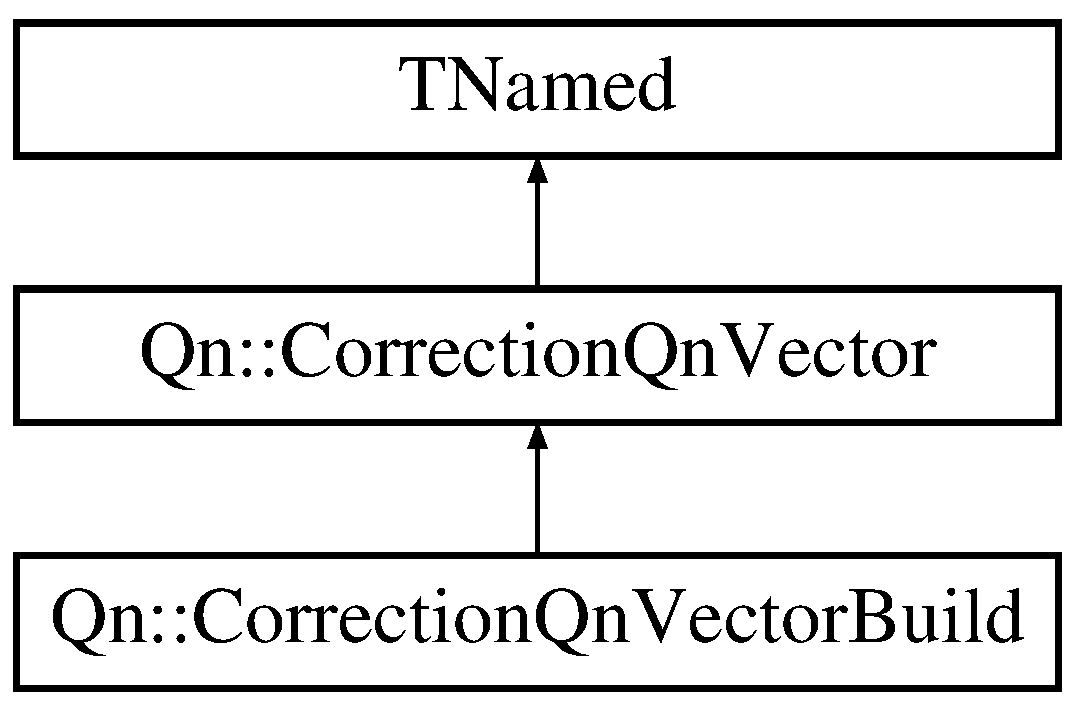
\includegraphics[height=3.000000cm]{classQn_1_1CorrectionQnVector}
\end{center}
\end{figure}
\subsection*{Public Types}
\begin{DoxyCompactItemize}
\item 
enum \mbox{\hyperlink{classQn_1_1CorrectionQnVector_a2998fe4babb716c57848c8c73b24a398}{Normalization}} \{ \mbox{\hyperlink{classQn_1_1CorrectionQnVector_a2998fe4babb716c57848c8c73b24a398ab50339a10e1de285ac99d4c3990b8693}{Normalization\+::\+N\+O\+NE}}, 
\mbox{\hyperlink{classQn_1_1CorrectionQnVector_a2998fe4babb716c57848c8c73b24a398a465f35d0481ebf03b978c3bd9eb1e5b6}{Normalization\+::\+S\+Q\+R\+T\+\_\+M}}, 
\mbox{\hyperlink{classQn_1_1CorrectionQnVector_a2998fe4babb716c57848c8c73b24a398a69691c7bdcc3ce6d5d8a1361f22d04ac}{Normalization\+::M}}, 
\mbox{\hyperlink{classQn_1_1CorrectionQnVector_a2998fe4babb716c57848c8c73b24a398aba1a4ef58204f0da36291466025d7533}{Normalization\+::\+M\+A\+G\+N\+I\+T\+U\+DE}}
 \}
\end{DoxyCompactItemize}
\subsection*{Public Member Functions}
\begin{DoxyCompactItemize}
\item 
\mbox{\Hypertarget{classQn_1_1CorrectionQnVector_a28007d64a859512c43ac7e7f1a477d9e}\label{classQn_1_1CorrectionQnVector_a28007d64a859512c43ac7e7f1a477d9e}} 
\mbox{\hyperlink{classQn_1_1CorrectionQnVector_a28007d64a859512c43ac7e7f1a477d9e}{Correction\+Qn\+Vector}} ()
\begin{DoxyCompactList}\small\item\em Default constructor. \end{DoxyCompactList}\item 
\mbox{\hyperlink{classQn_1_1CorrectionQnVector_a4cb37d125c255b433565248dd0054f27}{Correction\+Qn\+Vector}} (const char $\ast$name, Int\+\_\+t n\+No\+Of\+Harmonics, Int\+\_\+t $\ast$harmonic\+Map=N\+U\+LL)
\item 
\mbox{\hyperlink{classQn_1_1CorrectionQnVector_a9463528777b5ad1dbe0f68f4d575d7fa}{Correction\+Qn\+Vector}} (const char $\ast$name, Int\+\_\+t n\+Extract\+Multiple\+Of, Int\+\_\+t n\+No\+Of\+Harmonics, Int\+\_\+t $\ast$harmonic\+Map)
\item 
\mbox{\hyperlink{classQn_1_1CorrectionQnVector_a667da9b9391dc7b3aeb45dfbdbf35c31}{Correction\+Qn\+Vector}} (const \mbox{\hyperlink{classQn_1_1CorrectionQnVector}{Correction\+Qn\+Vector}} \&Q)
\item 
\mbox{\hyperlink{classQn_1_1CorrectionQnVector_af1d34ffbe05b79eb8125bcf44033b790}{Correction\+Qn\+Vector}} (Int\+\_\+t n\+Divisor, const \mbox{\hyperlink{classQn_1_1CorrectionQnVector}{Correction\+Qn\+Vector}} \&Q)
\item 
\mbox{\Hypertarget{classQn_1_1CorrectionQnVector_a51d5ab05176552adff4e7bce1612864a}\label{classQn_1_1CorrectionQnVector_a51d5ab05176552adff4e7bce1612864a}} 
virtual \mbox{\hyperlink{classQn_1_1CorrectionQnVector_a51d5ab05176552adff4e7bce1612864a}{$\sim$\+Correction\+Qn\+Vector}} ()
\begin{DoxyCompactList}\small\item\em Default destructor. \end{DoxyCompactList}\item 
void \mbox{\hyperlink{classQn_1_1CorrectionQnVector_a6fcf855ca57bab1752ebb8098aa8da8d}{Activate\+Harmonic}} (Int\+\_\+t harmonic)
\item 
Int\+\_\+t \mbox{\hyperlink{classQn_1_1CorrectionQnVector_a4da8a1b6a2f12c2393ae86b5fa19b0ae}{Get\+No\+Of\+Harmonics}} () const
\item 
void \mbox{\hyperlink{classQn_1_1CorrectionQnVector_af41ace21d8328373d0496ea68e5a468c}{Get\+Harmonics\+Map}} (Int\+\_\+t $\ast$harmonic\+Map) const
\item 
Int\+\_\+t \mbox{\hyperlink{classQn_1_1CorrectionQnVector_ac5110bb9d339c2387e0cfd411c534997}{Get\+First\+Harmonic}} () const
\item 
Int\+\_\+t \mbox{\hyperlink{classQn_1_1CorrectionQnVector_a9b0c28b62017cc7a369b39bbbbc2301a}{Get\+Next\+Harmonic}} (Int\+\_\+t harmonic) const
\item 
Int\+\_\+t \mbox{\hyperlink{classQn_1_1CorrectionQnVector_a083f96d5886c8ea53681a125043e8150}{Get\+Harmonic\+Multiplier}} () const
\item 
virtual void \mbox{\hyperlink{classQn_1_1CorrectionQnVector_a6de477e3cecce7c5f5b9212ecbafea59}{Set\+Qx}} (Int\+\_\+t harmonic, Float\+\_\+t qx)
\item 
virtual void \mbox{\hyperlink{classQn_1_1CorrectionQnVector_af0ac581e943fe88b0a94838c670f2c4d}{Set\+Qy}} (Int\+\_\+t harmonic, Float\+\_\+t qy)
\item 
virtual void \mbox{\hyperlink{classQn_1_1CorrectionQnVector_a71b91d6c9ed672d997f91421192974f6}{Set\+Good}} (Bool\+\_\+t good)
\item 
virtual void \mbox{\hyperlink{classQn_1_1CorrectionQnVector_acc6c39c8247f6f43c13c1886c3a5bcd4}{Set\+Harmonic\+Multiplier}} (Int\+\_\+t m)
\item 
void \mbox{\hyperlink{classQn_1_1CorrectionQnVector_acd45aaacfb58f260eb8b0102cc46ef05}{Set}} (\mbox{\hyperlink{classQn_1_1CorrectionQnVector}{Correction\+Qn\+Vector}} $\ast$Qn, Bool\+\_\+t changename)
\item 
void \mbox{\hyperlink{classQn_1_1CorrectionQnVector_a8e2e40587de98b65ec6b89ce82fb63a7}{Normalize}} ()
\item 
Float\+\_\+t \mbox{\hyperlink{classQn_1_1CorrectionQnVector_ad8b5dd08034a692eee13f2baa4d42269}{Length}} (Int\+\_\+t harmonic) const
\item 
Float\+\_\+t \mbox{\hyperlink{classQn_1_1CorrectionQnVector_abf503da4fb27fc1e046fbd195a841926}{Qx\+Norm}} (Int\+\_\+t harmonic) const
\item 
Float\+\_\+t \mbox{\hyperlink{classQn_1_1CorrectionQnVector_af8c17655a61268b003515554cc146814}{Qy\+Norm}} (Int\+\_\+t harmonic) const
\item 
\mbox{\Hypertarget{classQn_1_1CorrectionQnVector_ab157bf86ea39a70bba7f3fd1534d0166}\label{classQn_1_1CorrectionQnVector_ab157bf86ea39a70bba7f3fd1534d0166}} 
virtual void \mbox{\hyperlink{classQn_1_1CorrectionQnVector_ab157bf86ea39a70bba7f3fd1534d0166}{Reset}} ()
\begin{DoxyCompactList}\small\item\em Resets the Q vector values without touching the structure. \end{DoxyCompactList}\item 
Float\+\_\+t \mbox{\hyperlink{classQn_1_1CorrectionQnVector_a7a72044374f9040ebfdc364e574f0cca}{Qx}} (Int\+\_\+t harmonic) const
\item 
Float\+\_\+t \mbox{\hyperlink{classQn_1_1CorrectionQnVector_adf6c66295489c2638e9f692a77f6ca9b}{Qy}} (Int\+\_\+t harmonic) const
\item 
Bool\+\_\+t \mbox{\hyperlink{classQn_1_1CorrectionQnVector_a314e710f1e4f6d09ab19907c5ecd48dc}{Is\+Good\+Quality}} () const
\item 
Int\+\_\+t \mbox{\hyperlink{classQn_1_1CorrectionQnVector_ab182d3ac68a795f5732daa83ae2f7417}{GetN}} () const
\item 
Float\+\_\+t \mbox{\hyperlink{classQn_1_1CorrectionQnVector_a77ec3056318b215938cac926cd9cb3c2}{Get\+Sum\+Of\+Weights}} () const
\item 
Double\+\_\+t \mbox{\hyperlink{classQn_1_1CorrectionQnVector_afa869b89c2b19a6f473572e45e6c33ec}{Event\+Plane}} (Int\+\_\+t harmonic) const
\item 
virtual void \mbox{\hyperlink{classQn_1_1CorrectionQnVector_a859e8ffe20c7a607f67bb95f8c85b9e9}{Print}} (Option\+\_\+t $\ast$) const
\item 
\mbox{\Hypertarget{classQn_1_1CorrectionQnVector_a70ce863e91181bcd6a259453aebb12d9}\label{classQn_1_1CorrectionQnVector_a70ce863e91181bcd6a259453aebb12d9}} 
\mbox{\hyperlink{classQn_1_1CorrectionQnVector}{Correction\+Qn\+Vector}} \& \mbox{\hyperlink{classQn_1_1CorrectionQnVector_a70ce863e91181bcd6a259453aebb12d9}{operator=}} (const \mbox{\hyperlink{classQn_1_1CorrectionQnVector}{Correction\+Qn\+Vector}} \&Qn)
\begin{DoxyCompactList}\small\item\em Assignment operator. \end{DoxyCompactList}\end{DoxyCompactItemize}
\subsection*{Protected Attributes}
\begin{DoxyCompactItemize}
\item 
\mbox{\Hypertarget{classQn_1_1CorrectionQnVector_a2ae659e3a1bb05acdc53befd228f8e21}\label{classQn_1_1CorrectionQnVector_a2ae659e3a1bb05acdc53befd228f8e21}} 
Float\+\_\+t \mbox{\hyperlink{classQn_1_1CorrectionQnVector_a2ae659e3a1bb05acdc53befd228f8e21}{f\+QnX}} \mbox{[}M\+A\+X\+H\+A\+R\+M\+O\+N\+I\+C\+N\+U\+M\+B\+E\+R\+S\+U\+P\+P\+O\+R\+T\+ED+1\mbox{]}
\begin{DoxyCompactList}\small\item\em the Q vector X component for each harmonic \end{DoxyCompactList}\item 
\mbox{\Hypertarget{classQn_1_1CorrectionQnVector_a633fc0ceee269c905d852d12adb8f767}\label{classQn_1_1CorrectionQnVector_a633fc0ceee269c905d852d12adb8f767}} 
Float\+\_\+t \mbox{\hyperlink{classQn_1_1CorrectionQnVector_a633fc0ceee269c905d852d12adb8f767}{f\+QnY}} \mbox{[}M\+A\+X\+H\+A\+R\+M\+O\+N\+I\+C\+N\+U\+M\+B\+E\+R\+S\+U\+P\+P\+O\+R\+T\+ED+1\mbox{]}
\begin{DoxyCompactList}\small\item\em the Q vector Y component for each harmonic \end{DoxyCompactList}\item 
\mbox{\Hypertarget{classQn_1_1CorrectionQnVector_ad37b7d348ec4ba631a3829fe1dde8709}\label{classQn_1_1CorrectionQnVector_ad37b7d348ec4ba631a3829fe1dde8709}} 
Int\+\_\+t \mbox{\hyperlink{classQn_1_1CorrectionQnVector_ad37b7d348ec4ba631a3829fe1dde8709}{f\+Highest\+Harmonic}}
\begin{DoxyCompactList}\small\item\em the highest harmonic number handled \end{DoxyCompactList}\item 
\mbox{\Hypertarget{classQn_1_1CorrectionQnVector_a11c90eb2e5d463bbb6669bf1cd845b71}\label{classQn_1_1CorrectionQnVector_a11c90eb2e5d463bbb6669bf1cd845b71}} 
U\+Int\+\_\+t \mbox{\hyperlink{classQn_1_1CorrectionQnVector_a11c90eb2e5d463bbb6669bf1cd845b71}{f\+Harmonic\+Mask}}
\begin{DoxyCompactList}\small\item\em the mask for the supported harmonics \end{DoxyCompactList}\item 
\mbox{\Hypertarget{classQn_1_1CorrectionQnVector_a368a0eb951505630ae8ba7d85e46671c}\label{classQn_1_1CorrectionQnVector_a368a0eb951505630ae8ba7d85e46671c}} 
Bool\+\_\+t \mbox{\hyperlink{classQn_1_1CorrectionQnVector_a368a0eb951505630ae8ba7d85e46671c}{f\+Good\+Quality}}
\begin{DoxyCompactList}\small\item\em \mbox{\hyperlink{namespaceQn}{Qn}} vector good quality flag. \end{DoxyCompactList}\item 
\mbox{\Hypertarget{classQn_1_1CorrectionQnVector_a66810d5fcac23b630b40c673a6804b26}\label{classQn_1_1CorrectionQnVector_a66810d5fcac23b630b40c673a6804b26}} 
Int\+\_\+t \mbox{\hyperlink{classQn_1_1CorrectionQnVector_a66810d5fcac23b630b40c673a6804b26}{fN}}
\begin{DoxyCompactList}\small\item\em number of elements used for \mbox{\hyperlink{namespaceQn}{Qn}} vector building \end{DoxyCompactList}\item 
\mbox{\Hypertarget{classQn_1_1CorrectionQnVector_ac85bb3bbe9a52f15ad330fe59724f0f8}\label{classQn_1_1CorrectionQnVector_ac85bb3bbe9a52f15ad330fe59724f0f8}} 
Float\+\_\+t \mbox{\hyperlink{classQn_1_1CorrectionQnVector_ac85bb3bbe9a52f15ad330fe59724f0f8}{f\+SumW}}
\begin{DoxyCompactList}\small\item\em the sum of weights \end{DoxyCompactList}\item 
\mbox{\Hypertarget{classQn_1_1CorrectionQnVector_afeff0835afa33a26d719f1af506ea4b1}\label{classQn_1_1CorrectionQnVector_afeff0835afa33a26d719f1af506ea4b1}} 
Int\+\_\+t \mbox{\hyperlink{classQn_1_1CorrectionQnVector_afeff0835afa33a26d719f1af506ea4b1}{f\+Harmonic\+Multiplier}}
\begin{DoxyCompactList}\small\item\em the multiplier of the different harmonics \end{DoxyCompactList}\end{DoxyCompactItemize}
\subsection*{Static Protected Attributes}
\begin{DoxyCompactItemize}
\item 
\mbox{\Hypertarget{classQn_1_1CorrectionQnVector_ae6b54b512ea4942bbed53cb012980035}\label{classQn_1_1CorrectionQnVector_ae6b54b512ea4942bbed53cb012980035}} 
static const Float\+\_\+t \mbox{\hyperlink{classQn_1_1CorrectionQnVector_ae6b54b512ea4942bbed53cb012980035}{f\+Minimum\+Significant\+Value}} = 1e-\/6
\begin{DoxyCompactList}\small\item\em the minimum value that will be considered as meaningful for processing \end{DoxyCompactList}\item 
static const U\+Int\+\_\+t \mbox{\hyperlink{classQn_1_1CorrectionQnVector_a4dd6b60f412516d586b204f63350ab5d}{harmonic\+Number\+Mask}} \mbox{[}$\,$\mbox{]}
\begin{DoxyCompactList}\small\item\em Mask for each external harmonic number. \end{DoxyCompactList}\end{DoxyCompactItemize}


\subsection{Member Enumeration Documentation}
\mbox{\Hypertarget{classQn_1_1CorrectionQnVector_a2998fe4babb716c57848c8c73b24a398}\label{classQn_1_1CorrectionQnVector_a2998fe4babb716c57848c8c73b24a398}} 
\index{Qn\+::\+Correction\+Qn\+Vector@{Qn\+::\+Correction\+Qn\+Vector}!Normalization@{Normalization}}
\index{Normalization@{Normalization}!Qn\+::\+Correction\+Qn\+Vector@{Qn\+::\+Correction\+Qn\+Vector}}
\subsubsection{\texorpdfstring{Normalization}{Normalization}}
{\footnotesize\ttfamily enum \mbox{\hyperlink{classQn_1_1CorrectionQnVector_a2998fe4babb716c57848c8c73b24a398}{Qn\+::\+Correction\+Qn\+Vector\+::\+Normalization}}\hspace{0.3cm}{\ttfamily [strong]}}

\begin{DoxyEnumFields}{Enumerator}
\raisebox{\heightof{T}}[0pt][0pt]{\index{N\+O\+NE@{N\+O\+NE}!Qn\+::\+Correction\+Qn\+Vector@{Qn\+::\+Correction\+Qn\+Vector}}\index{Qn\+::\+Correction\+Qn\+Vector@{Qn\+::\+Correction\+Qn\+Vector}!N\+O\+NE@{N\+O\+NE}}}\mbox{\Hypertarget{classQn_1_1CorrectionQnVector_a2998fe4babb716c57848c8c73b24a398ab50339a10e1de285ac99d4c3990b8693}\label{classQn_1_1CorrectionQnVector_a2998fe4babb716c57848c8c73b24a398ab50339a10e1de285ac99d4c3990b8693}} 
N\+O\+NE&$ \mbox{Q'} = \mbox{Q}$ \\
\hline

\raisebox{\heightof{T}}[0pt][0pt]{\index{S\+Q\+R\+T\+\_\+M@{S\+Q\+R\+T\+\_\+M}!Qn\+::\+Correction\+Qn\+Vector@{Qn\+::\+Correction\+Qn\+Vector}}\index{Qn\+::\+Correction\+Qn\+Vector@{Qn\+::\+Correction\+Qn\+Vector}!S\+Q\+R\+T\+\_\+M@{S\+Q\+R\+T\+\_\+M}}}\mbox{\Hypertarget{classQn_1_1CorrectionQnVector_a2998fe4babb716c57848c8c73b24a398a465f35d0481ebf03b978c3bd9eb1e5b6}\label{classQn_1_1CorrectionQnVector_a2998fe4babb716c57848c8c73b24a398a465f35d0481ebf03b978c3bd9eb1e5b6}} 
S\+Q\+R\+T\+\_\+M&$ \mbox{Q'} = \frac{\mbox{Q}}{\sqrt{\mbox{M}}} $ \\
\hline

\raisebox{\heightof{T}}[0pt][0pt]{\index{M@{M}!Qn\+::\+Correction\+Qn\+Vector@{Qn\+::\+Correction\+Qn\+Vector}}\index{Qn\+::\+Correction\+Qn\+Vector@{Qn\+::\+Correction\+Qn\+Vector}!M@{M}}}\mbox{\Hypertarget{classQn_1_1CorrectionQnVector_a2998fe4babb716c57848c8c73b24a398a69691c7bdcc3ce6d5d8a1361f22d04ac}\label{classQn_1_1CorrectionQnVector_a2998fe4babb716c57848c8c73b24a398a69691c7bdcc3ce6d5d8a1361f22d04ac}} 
M&$ \mbox{Q'} = \frac{\mbox{Q}}{\mbox{M}} $ \\
\hline

\raisebox{\heightof{T}}[0pt][0pt]{\index{M\+A\+G\+N\+I\+T\+U\+DE@{M\+A\+G\+N\+I\+T\+U\+DE}!Qn\+::\+Correction\+Qn\+Vector@{Qn\+::\+Correction\+Qn\+Vector}}\index{Qn\+::\+Correction\+Qn\+Vector@{Qn\+::\+Correction\+Qn\+Vector}!M\+A\+G\+N\+I\+T\+U\+DE@{M\+A\+G\+N\+I\+T\+U\+DE}}}\mbox{\Hypertarget{classQn_1_1CorrectionQnVector_a2998fe4babb716c57848c8c73b24a398aba1a4ef58204f0da36291466025d7533}\label{classQn_1_1CorrectionQnVector_a2998fe4babb716c57848c8c73b24a398aba1a4ef58204f0da36291466025d7533}} 
M\+A\+G\+N\+I\+T\+U\+DE&$ \mbox{Q'} = \frac{\mbox{Q}}{|\mbox{Q}|} $ \\
\hline

\end{DoxyEnumFields}


\subsection{Constructor \& Destructor Documentation}
\mbox{\Hypertarget{classQn_1_1CorrectionQnVector_a4cb37d125c255b433565248dd0054f27}\label{classQn_1_1CorrectionQnVector_a4cb37d125c255b433565248dd0054f27}} 
\index{Qn\+::\+Correction\+Qn\+Vector@{Qn\+::\+Correction\+Qn\+Vector}!Correction\+Qn\+Vector@{Correction\+Qn\+Vector}}
\index{Correction\+Qn\+Vector@{Correction\+Qn\+Vector}!Qn\+::\+Correction\+Qn\+Vector@{Qn\+::\+Correction\+Qn\+Vector}}
\subsubsection{\texorpdfstring{Correction\+Qn\+Vector()}{CorrectionQnVector()}\hspace{0.1cm}{\footnotesize\ttfamily [1/4]}}
{\footnotesize\ttfamily Qn\+::\+Correction\+Qn\+Vector\+::\+Correction\+Qn\+Vector (\begin{DoxyParamCaption}\item[{const char $\ast$}]{name,  }\item[{Int\+\_\+t}]{n\+No\+Of\+Harmonics,  }\item[{Int\+\_\+t $\ast$}]{harmonic\+Map = {\ttfamily NULL} }\end{DoxyParamCaption})}

Normal constructor

For each harmonic number the Q vector is initialized The Q vectors are organized to support external harmonic number. By default the external harmonic number is always considered to start by one. If no map is passed as parameter the external harmonic numbers are considered as\+: 1, 2, ..., n\+No\+Of\+Harmonic. If the user wants a different assignment he has to provide an ordered map, for instance\+: four harmonics with external harmonic numbers 2, 4, 6 and 8 will require n\+No\+Of\+Harmonics = 4 and harmonic\+Map = \mbox{[}2, 4, 6, 8\mbox{]}.

A check on the asked number of harmonics is made for having it within current implementation limits.


\begin{DoxyParams}{Parameters}
{\em name} & the name of the \mbox{\hyperlink{namespaceQn}{Qn}} vector. Identifies its origin \\
\hline
{\em n\+No\+Of\+Harmonics} & the desired number of harmonics \\
\hline
{\em harmonic\+Map} & ordered array with the external number of the harmonics \\
\hline
\end{DoxyParams}
\mbox{\Hypertarget{classQn_1_1CorrectionQnVector_a9463528777b5ad1dbe0f68f4d575d7fa}\label{classQn_1_1CorrectionQnVector_a9463528777b5ad1dbe0f68f4d575d7fa}} 
\index{Qn\+::\+Correction\+Qn\+Vector@{Qn\+::\+Correction\+Qn\+Vector}!Correction\+Qn\+Vector@{Correction\+Qn\+Vector}}
\index{Correction\+Qn\+Vector@{Correction\+Qn\+Vector}!Qn\+::\+Correction\+Qn\+Vector@{Qn\+::\+Correction\+Qn\+Vector}}
\subsubsection{\texorpdfstring{Correction\+Qn\+Vector()}{CorrectionQnVector()}\hspace{0.1cm}{\footnotesize\ttfamily [2/4]}}
{\footnotesize\ttfamily Qn\+::\+Correction\+Qn\+Vector\+::\+Correction\+Qn\+Vector (\begin{DoxyParamCaption}\item[{const char $\ast$}]{name,  }\item[{Int\+\_\+t}]{n\+Divisor,  }\item[{Int\+\_\+t}]{n\+No\+Of\+Harmonics,  }\item[{Int\+\_\+t $\ast$}]{harmonic\+Map }\end{DoxyParamCaption})}

Normal constructor for supporting a subset of the harmonics passed

For each integer harmonic number after dividing by the divisor the Q vector is initialized The Q vectors are organized to support external harmonic number. Only support for the desired harmonic multiples is build. If harmonic\+Map = \mbox{[}1, 2, 3, 4, 6, 8\mbox{]} is passed and the divisor is two then the created \mbox{\hyperlink{namespaceQn}{Qn}} vector has support for the harmonics numbers 1, 2, 3 and 4.

A check on the asked number of harmonics is made for having it within current implementation limits.


\begin{DoxyParams}{Parameters}
{\em name} & the name of the \mbox{\hyperlink{namespaceQn}{Qn}} vector. Identifies its origin \\
\hline
{\em n\+Divisor} & the divisor of the harmonic number for getting the harmonic we want to create support for \\
\hline
{\em n\+No\+Of\+Harmonics} & the number of harmonics passed within the map \\
\hline
{\em harmonic\+Map} & ordered array with the external number of the harmonics \\
\hline
\end{DoxyParams}
\mbox{\Hypertarget{classQn_1_1CorrectionQnVector_a667da9b9391dc7b3aeb45dfbdbf35c31}\label{classQn_1_1CorrectionQnVector_a667da9b9391dc7b3aeb45dfbdbf35c31}} 
\index{Qn\+::\+Correction\+Qn\+Vector@{Qn\+::\+Correction\+Qn\+Vector}!Correction\+Qn\+Vector@{Correction\+Qn\+Vector}}
\index{Correction\+Qn\+Vector@{Correction\+Qn\+Vector}!Qn\+::\+Correction\+Qn\+Vector@{Qn\+::\+Correction\+Qn\+Vector}}
\subsubsection{\texorpdfstring{Correction\+Qn\+Vector()}{CorrectionQnVector()}\hspace{0.1cm}{\footnotesize\ttfamily [3/4]}}
{\footnotesize\ttfamily Qn\+::\+Correction\+Qn\+Vector\+::\+Correction\+Qn\+Vector (\begin{DoxyParamCaption}\item[{const \mbox{\hyperlink{classQn_1_1CorrectionQnVector}{Correction\+Qn\+Vector}} \&}]{Qn }\end{DoxyParamCaption})}

Copy constructor 
\begin{DoxyParams}{Parameters}
{\em \mbox{\hyperlink{namespaceQn}{Qn}}} & the Q vector object to copy after construction \\
\hline
\end{DoxyParams}
\mbox{\Hypertarget{classQn_1_1CorrectionQnVector_af1d34ffbe05b79eb8125bcf44033b790}\label{classQn_1_1CorrectionQnVector_af1d34ffbe05b79eb8125bcf44033b790}} 
\index{Qn\+::\+Correction\+Qn\+Vector@{Qn\+::\+Correction\+Qn\+Vector}!Correction\+Qn\+Vector@{Correction\+Qn\+Vector}}
\index{Correction\+Qn\+Vector@{Correction\+Qn\+Vector}!Qn\+::\+Correction\+Qn\+Vector@{Qn\+::\+Correction\+Qn\+Vector}}
\subsubsection{\texorpdfstring{Correction\+Qn\+Vector()}{CorrectionQnVector()}\hspace{0.1cm}{\footnotesize\ttfamily [4/4]}}
{\footnotesize\ttfamily Qn\+::\+Correction\+Qn\+Vector\+::\+Correction\+Qn\+Vector (\begin{DoxyParamCaption}\item[{Int\+\_\+t}]{n\+Divisor,  }\item[{const \mbox{\hyperlink{classQn_1_1CorrectionQnVector}{Correction\+Qn\+Vector}} \&}]{Q }\end{DoxyParamCaption})}

Copy constructor for supporting a subset of the harmonics passed

For each integer harmonic number after dividing by the divisor the Q vector is copied


\begin{DoxyParams}{Parameters}
{\em n\+Divisor} & the divisor of the harmonic number for getting the harmonic we want to create support for \\
\hline
{\em Q} & the Q vector object to copy after construction \\
\hline
\end{DoxyParams}


\subsection{Member Function Documentation}
\mbox{\Hypertarget{classQn_1_1CorrectionQnVector_a6fcf855ca57bab1752ebb8098aa8da8d}\label{classQn_1_1CorrectionQnVector_a6fcf855ca57bab1752ebb8098aa8da8d}} 
\index{Qn\+::\+Correction\+Qn\+Vector@{Qn\+::\+Correction\+Qn\+Vector}!Activate\+Harmonic@{Activate\+Harmonic}}
\index{Activate\+Harmonic@{Activate\+Harmonic}!Qn\+::\+Correction\+Qn\+Vector@{Qn\+::\+Correction\+Qn\+Vector}}
\subsubsection{\texorpdfstring{Activate\+Harmonic()}{ActivateHarmonic()}}
{\footnotesize\ttfamily void Qn\+::\+Correction\+Qn\+Vector\+::\+Activate\+Harmonic (\begin{DoxyParamCaption}\item[{Int\+\_\+t}]{harmonic }\end{DoxyParamCaption})}

Activates the desired harmonic for processing

A check on the asked harmonic is made for having it within current implementation limits.

If the harmonic was not active its Q vector is initialized.


\begin{DoxyParams}{Parameters}
{\em harmonic} & the intended harmonic \\
\hline
\end{DoxyParams}
\mbox{\Hypertarget{classQn_1_1CorrectionQnVector_afa869b89c2b19a6f473572e45e6c33ec}\label{classQn_1_1CorrectionQnVector_afa869b89c2b19a6f473572e45e6c33ec}} 
\index{Qn\+::\+Correction\+Qn\+Vector@{Qn\+::\+Correction\+Qn\+Vector}!Event\+Plane@{Event\+Plane}}
\index{Event\+Plane@{Event\+Plane}!Qn\+::\+Correction\+Qn\+Vector@{Qn\+::\+Correction\+Qn\+Vector}}
\subsubsection{\texorpdfstring{Event\+Plane()}{EventPlane()}}
{\footnotesize\ttfamily Double\+\_\+t Qn\+::\+Correction\+Qn\+Vector\+::\+Event\+Plane (\begin{DoxyParamCaption}\item[{Int\+\_\+t}]{harmonic }\end{DoxyParamCaption}) const}

Gets the event plane for the asked harmonic

A check for significant values is made. Not passing them returns 0.\+0. 
\begin{DoxyParams}{Parameters}
{\em harmonic} & the intended harmonic number \\
\hline
\end{DoxyParams}
\begin{DoxyReturn}{Returns}
The event plane according to $\frac{1}{h}\tan^{-1}{\frac{Qh_X}{Qh_Y}}$ 
\end{DoxyReturn}
\mbox{\Hypertarget{classQn_1_1CorrectionQnVector_ac5110bb9d339c2387e0cfd411c534997}\label{classQn_1_1CorrectionQnVector_ac5110bb9d339c2387e0cfd411c534997}} 
\index{Qn\+::\+Correction\+Qn\+Vector@{Qn\+::\+Correction\+Qn\+Vector}!Get\+First\+Harmonic@{Get\+First\+Harmonic}}
\index{Get\+First\+Harmonic@{Get\+First\+Harmonic}!Qn\+::\+Correction\+Qn\+Vector@{Qn\+::\+Correction\+Qn\+Vector}}
\subsubsection{\texorpdfstring{Get\+First\+Harmonic()}{GetFirstHarmonic()}}
{\footnotesize\ttfamily Int\+\_\+t Qn\+::\+Correction\+Qn\+Vector\+::\+Get\+First\+Harmonic (\begin{DoxyParamCaption}{ }\end{DoxyParamCaption}) const\hspace{0.3cm}{\ttfamily [inline]}}

Get the number of the first harmonic used \begin{DoxyReturn}{Returns}
the number of the first harmonic handled by the Q vector, -\/1 if none 
\end{DoxyReturn}
\mbox{\Hypertarget{classQn_1_1CorrectionQnVector_a083f96d5886c8ea53681a125043e8150}\label{classQn_1_1CorrectionQnVector_a083f96d5886c8ea53681a125043e8150}} 
\index{Qn\+::\+Correction\+Qn\+Vector@{Qn\+::\+Correction\+Qn\+Vector}!Get\+Harmonic\+Multiplier@{Get\+Harmonic\+Multiplier}}
\index{Get\+Harmonic\+Multiplier@{Get\+Harmonic\+Multiplier}!Qn\+::\+Correction\+Qn\+Vector@{Qn\+::\+Correction\+Qn\+Vector}}
\subsubsection{\texorpdfstring{Get\+Harmonic\+Multiplier()}{GetHarmonicMultiplier()}}
{\footnotesize\ttfamily Int\+\_\+t Qn\+::\+Correction\+Qn\+Vector\+::\+Get\+Harmonic\+Multiplier (\begin{DoxyParamCaption}{ }\end{DoxyParamCaption}) const\hspace{0.3cm}{\ttfamily [inline]}}

Get the harmonic multiplier \begin{DoxyReturn}{Returns}
the harmonic multiplier 
\end{DoxyReturn}
\mbox{\Hypertarget{classQn_1_1CorrectionQnVector_af41ace21d8328373d0496ea68e5a468c}\label{classQn_1_1CorrectionQnVector_af41ace21d8328373d0496ea68e5a468c}} 
\index{Qn\+::\+Correction\+Qn\+Vector@{Qn\+::\+Correction\+Qn\+Vector}!Get\+Harmonics\+Map@{Get\+Harmonics\+Map}}
\index{Get\+Harmonics\+Map@{Get\+Harmonics\+Map}!Qn\+::\+Correction\+Qn\+Vector@{Qn\+::\+Correction\+Qn\+Vector}}
\subsubsection{\texorpdfstring{Get\+Harmonics\+Map()}{GetHarmonicsMap()}}
{\footnotesize\ttfamily void Qn\+::\+Correction\+Qn\+Vector\+::\+Get\+Harmonics\+Map (\begin{DoxyParamCaption}\item[{Int\+\_\+t $\ast$}]{harmonic\+Map\+Store }\end{DoxyParamCaption}) const}

Get the harmonic map handled by the Q vector The pointer passed should allow writing in at least the number of harmonics used so, use first \mbox{\hyperlink{classQn_1_1CorrectionQnVector_a4da8a1b6a2f12c2393ae86b5fa19b0ae}{Get\+No\+Of\+Harmonics()}} to get that


\begin{DoxyParams}{Parameters}
{\em harmonic\+Map\+Store} & pointer to where to store the harmonic map \\
\hline
\end{DoxyParams}
\mbox{\Hypertarget{classQn_1_1CorrectionQnVector_ab182d3ac68a795f5732daa83ae2f7417}\label{classQn_1_1CorrectionQnVector_ab182d3ac68a795f5732daa83ae2f7417}} 
\index{Qn\+::\+Correction\+Qn\+Vector@{Qn\+::\+Correction\+Qn\+Vector}!GetN@{GetN}}
\index{GetN@{GetN}!Qn\+::\+Correction\+Qn\+Vector@{Qn\+::\+Correction\+Qn\+Vector}}
\subsubsection{\texorpdfstring{Get\+N()}{GetN()}}
{\footnotesize\ttfamily Int\+\_\+t Qn\+::\+Correction\+Qn\+Vector\+::\+GetN (\begin{DoxyParamCaption}{ }\end{DoxyParamCaption}) const\hspace{0.3cm}{\ttfamily [inline]}}

Gets the number of elements that were used for Q vector building \begin{DoxyReturn}{Returns}
number of elements 
\end{DoxyReturn}
\mbox{\Hypertarget{classQn_1_1CorrectionQnVector_a9b0c28b62017cc7a369b39bbbbc2301a}\label{classQn_1_1CorrectionQnVector_a9b0c28b62017cc7a369b39bbbbc2301a}} 
\index{Qn\+::\+Correction\+Qn\+Vector@{Qn\+::\+Correction\+Qn\+Vector}!Get\+Next\+Harmonic@{Get\+Next\+Harmonic}}
\index{Get\+Next\+Harmonic@{Get\+Next\+Harmonic}!Qn\+::\+Correction\+Qn\+Vector@{Qn\+::\+Correction\+Qn\+Vector}}
\subsubsection{\texorpdfstring{Get\+Next\+Harmonic()}{GetNextHarmonic()}}
{\footnotesize\ttfamily Int\+\_\+t Qn\+::\+Correction\+Qn\+Vector\+::\+Get\+Next\+Harmonic (\begin{DoxyParamCaption}\item[{Int\+\_\+t}]{harmonic }\end{DoxyParamCaption}) const\hspace{0.3cm}{\ttfamily [inline]}}

Get the next harmonic to the one passed as parameter 
\begin{DoxyParams}{Parameters}
{\em harmonic} & number to find the next one \\
\hline
\end{DoxyParams}
\begin{DoxyReturn}{Returns}
the number of the next to the passed harmonic, -\/1 if none 
\end{DoxyReturn}
\mbox{\Hypertarget{classQn_1_1CorrectionQnVector_a4da8a1b6a2f12c2393ae86b5fa19b0ae}\label{classQn_1_1CorrectionQnVector_a4da8a1b6a2f12c2393ae86b5fa19b0ae}} 
\index{Qn\+::\+Correction\+Qn\+Vector@{Qn\+::\+Correction\+Qn\+Vector}!Get\+No\+Of\+Harmonics@{Get\+No\+Of\+Harmonics}}
\index{Get\+No\+Of\+Harmonics@{Get\+No\+Of\+Harmonics}!Qn\+::\+Correction\+Qn\+Vector@{Qn\+::\+Correction\+Qn\+Vector}}
\subsubsection{\texorpdfstring{Get\+No\+Of\+Harmonics()}{GetNoOfHarmonics()}}
{\footnotesize\ttfamily Int\+\_\+t Qn\+::\+Correction\+Qn\+Vector\+::\+Get\+No\+Of\+Harmonics (\begin{DoxyParamCaption}{ }\end{DoxyParamCaption}) const}

Get the number of harmonics currently handled by the Q vector

\begin{DoxyReturn}{Returns}
the number of harmonics handled 
\end{DoxyReturn}
\mbox{\Hypertarget{classQn_1_1CorrectionQnVector_a77ec3056318b215938cac926cd9cb3c2}\label{classQn_1_1CorrectionQnVector_a77ec3056318b215938cac926cd9cb3c2}} 
\index{Qn\+::\+Correction\+Qn\+Vector@{Qn\+::\+Correction\+Qn\+Vector}!Get\+Sum\+Of\+Weights@{Get\+Sum\+Of\+Weights}}
\index{Get\+Sum\+Of\+Weights@{Get\+Sum\+Of\+Weights}!Qn\+::\+Correction\+Qn\+Vector@{Qn\+::\+Correction\+Qn\+Vector}}
\subsubsection{\texorpdfstring{Get\+Sum\+Of\+Weights()}{GetSumOfWeights()}}
{\footnotesize\ttfamily Float\+\_\+t Qn\+::\+Correction\+Qn\+Vector\+::\+Get\+Sum\+Of\+Weights (\begin{DoxyParamCaption}{ }\end{DoxyParamCaption}) const\hspace{0.3cm}{\ttfamily [inline]}}

Gets the sum of weights of the elements that were used for Q vector building \begin{DoxyReturn}{Returns}
sum of weights 
\end{DoxyReturn}
\mbox{\Hypertarget{classQn_1_1CorrectionQnVector_a314e710f1e4f6d09ab19907c5ecd48dc}\label{classQn_1_1CorrectionQnVector_a314e710f1e4f6d09ab19907c5ecd48dc}} 
\index{Qn\+::\+Correction\+Qn\+Vector@{Qn\+::\+Correction\+Qn\+Vector}!Is\+Good\+Quality@{Is\+Good\+Quality}}
\index{Is\+Good\+Quality@{Is\+Good\+Quality}!Qn\+::\+Correction\+Qn\+Vector@{Qn\+::\+Correction\+Qn\+Vector}}
\subsubsection{\texorpdfstring{Is\+Good\+Quality()}{IsGoodQuality()}}
{\footnotesize\ttfamily Bool\+\_\+t Qn\+::\+Correction\+Qn\+Vector\+::\+Is\+Good\+Quality (\begin{DoxyParamCaption}{ }\end{DoxyParamCaption}) const\hspace{0.3cm}{\ttfamily [inline]}}

Get the \mbox{\hyperlink{namespaceQn}{Qn}} vector quality flag \begin{DoxyReturn}{Returns}
\mbox{\hyperlink{namespaceQn}{Qn}} vector quality flag 
\end{DoxyReturn}
\mbox{\Hypertarget{classQn_1_1CorrectionQnVector_ad8b5dd08034a692eee13f2baa4d42269}\label{classQn_1_1CorrectionQnVector_ad8b5dd08034a692eee13f2baa4d42269}} 
\index{Qn\+::\+Correction\+Qn\+Vector@{Qn\+::\+Correction\+Qn\+Vector}!Length@{Length}}
\index{Length@{Length}!Qn\+::\+Correction\+Qn\+Vector@{Qn\+::\+Correction\+Qn\+Vector}}
\subsubsection{\texorpdfstring{Length()}{Length()}}
{\footnotesize\ttfamily Float\+\_\+t Qn\+::\+Correction\+Qn\+Vector\+::\+Length (\begin{DoxyParamCaption}\item[{Int\+\_\+t}]{harmonic }\end{DoxyParamCaption}) const\hspace{0.3cm}{\ttfamily [inline]}}

Provides the length of the Q vector for the considered harmonic 
\begin{DoxyParams}{Parameters}
{\em harmonic} & the intended harmonic \\
\hline
\end{DoxyParams}
\begin{DoxyReturn}{Returns}
the square root of components square sum 
\end{DoxyReturn}
\mbox{\Hypertarget{classQn_1_1CorrectionQnVector_a8e2e40587de98b65ec6b89ce82fb63a7}\label{classQn_1_1CorrectionQnVector_a8e2e40587de98b65ec6b89ce82fb63a7}} 
\index{Qn\+::\+Correction\+Qn\+Vector@{Qn\+::\+Correction\+Qn\+Vector}!Normalize@{Normalize}}
\index{Normalize@{Normalize}!Qn\+::\+Correction\+Qn\+Vector@{Qn\+::\+Correction\+Qn\+Vector}}
\subsubsection{\texorpdfstring{Normalize()}{Normalize()}}
{\footnotesize\ttfamily void Qn\+::\+Correction\+Qn\+Vector\+::\+Normalize (\begin{DoxyParamCaption}{ }\end{DoxyParamCaption})}

Normalize the Q vector to unit length \mbox{\Hypertarget{classQn_1_1CorrectionQnVector_a859e8ffe20c7a607f67bb95f8c85b9e9}\label{classQn_1_1CorrectionQnVector_a859e8ffe20c7a607f67bb95f8c85b9e9}} 
\index{Qn\+::\+Correction\+Qn\+Vector@{Qn\+::\+Correction\+Qn\+Vector}!Print@{Print}}
\index{Print@{Print}!Qn\+::\+Correction\+Qn\+Vector@{Qn\+::\+Correction\+Qn\+Vector}}
\subsubsection{\texorpdfstring{Print()}{Print()}}
{\footnotesize\ttfamily void Qn\+::\+Correction\+Qn\+Vector\+::\+Print (\begin{DoxyParamCaption}\item[{Option\+\_\+t $\ast$}]{ }\end{DoxyParamCaption}) const\hspace{0.3cm}{\ttfamily [virtual]}}

Print the \mbox{\hyperlink{namespaceQn}{Qn}} vector in a readable shape 

Reimplemented in \mbox{\hyperlink{classQn_1_1CorrectionQnVectorBuild_a8b767040ac4ae2472e8ce8f091b5ce88}{Qn\+::\+Correction\+Qn\+Vector\+Build}}.

\mbox{\Hypertarget{classQn_1_1CorrectionQnVector_a7a72044374f9040ebfdc364e574f0cca}\label{classQn_1_1CorrectionQnVector_a7a72044374f9040ebfdc364e574f0cca}} 
\index{Qn\+::\+Correction\+Qn\+Vector@{Qn\+::\+Correction\+Qn\+Vector}!Qx@{Qx}}
\index{Qx@{Qx}!Qn\+::\+Correction\+Qn\+Vector@{Qn\+::\+Correction\+Qn\+Vector}}
\subsubsection{\texorpdfstring{Qx()}{Qx()}}
{\footnotesize\ttfamily Float\+\_\+t Qn\+::\+Correction\+Qn\+Vector\+::\+Qx (\begin{DoxyParamCaption}\item[{Int\+\_\+t}]{harmonic }\end{DoxyParamCaption}) const\hspace{0.3cm}{\ttfamily [inline]}}

Gets the Q vector X component for the considered harmonic 
\begin{DoxyParams}{Parameters}
{\em harmonic} & the intended harmonic \\
\hline
\end{DoxyParams}
\begin{DoxyReturn}{Returns}
the Q vector X component 
\end{DoxyReturn}
\mbox{\Hypertarget{classQn_1_1CorrectionQnVector_abf503da4fb27fc1e046fbd195a841926}\label{classQn_1_1CorrectionQnVector_abf503da4fb27fc1e046fbd195a841926}} 
\index{Qn\+::\+Correction\+Qn\+Vector@{Qn\+::\+Correction\+Qn\+Vector}!Qx\+Norm@{Qx\+Norm}}
\index{Qx\+Norm@{Qx\+Norm}!Qn\+::\+Correction\+Qn\+Vector@{Qn\+::\+Correction\+Qn\+Vector}}
\subsubsection{\texorpdfstring{Qx\+Norm()}{QxNorm()}}
{\footnotesize\ttfamily Float\+\_\+t Qn\+::\+Correction\+Qn\+Vector\+::\+Qx\+Norm (\begin{DoxyParamCaption}\item[{Int\+\_\+t}]{harmonic }\end{DoxyParamCaption}) const\hspace{0.3cm}{\ttfamily [inline]}}

Provides the X component normalized to one of the Q vector for the considered harmonic A check for Q vector length significant value is made. Not passing it returns a zero value. 
\begin{DoxyParams}{Parameters}
{\em harmonic} & the intended harmonic \\
\hline
\end{DoxyParams}
\begin{DoxyReturn}{Returns}
X component of the normalized Q vector 
\end{DoxyReturn}
\mbox{\Hypertarget{classQn_1_1CorrectionQnVector_adf6c66295489c2638e9f692a77f6ca9b}\label{classQn_1_1CorrectionQnVector_adf6c66295489c2638e9f692a77f6ca9b}} 
\index{Qn\+::\+Correction\+Qn\+Vector@{Qn\+::\+Correction\+Qn\+Vector}!Qy@{Qy}}
\index{Qy@{Qy}!Qn\+::\+Correction\+Qn\+Vector@{Qn\+::\+Correction\+Qn\+Vector}}
\subsubsection{\texorpdfstring{Qy()}{Qy()}}
{\footnotesize\ttfamily Float\+\_\+t Qn\+::\+Correction\+Qn\+Vector\+::\+Qy (\begin{DoxyParamCaption}\item[{Int\+\_\+t}]{harmonic }\end{DoxyParamCaption}) const\hspace{0.3cm}{\ttfamily [inline]}}

Gets the Q vector Y component for the considered harmonic 
\begin{DoxyParams}{Parameters}
{\em harmonic} & the intended harmonic \\
\hline
\end{DoxyParams}
\begin{DoxyReturn}{Returns}
the Q vector Y component 
\end{DoxyReturn}
\mbox{\Hypertarget{classQn_1_1CorrectionQnVector_af8c17655a61268b003515554cc146814}\label{classQn_1_1CorrectionQnVector_af8c17655a61268b003515554cc146814}} 
\index{Qn\+::\+Correction\+Qn\+Vector@{Qn\+::\+Correction\+Qn\+Vector}!Qy\+Norm@{Qy\+Norm}}
\index{Qy\+Norm@{Qy\+Norm}!Qn\+::\+Correction\+Qn\+Vector@{Qn\+::\+Correction\+Qn\+Vector}}
\subsubsection{\texorpdfstring{Qy\+Norm()}{QyNorm()}}
{\footnotesize\ttfamily Float\+\_\+t Qn\+::\+Correction\+Qn\+Vector\+::\+Qy\+Norm (\begin{DoxyParamCaption}\item[{Int\+\_\+t}]{harmonic }\end{DoxyParamCaption}) const\hspace{0.3cm}{\ttfamily [inline]}}

Provides the Y component normalized to one of the Q vector for the considered harmonic A check for Q vector length significant value is made. Not passing it returns a zero value. 
\begin{DoxyParams}{Parameters}
{\em harmonic} & the intended harmonic \\
\hline
\end{DoxyParams}
\begin{DoxyReturn}{Returns}
Y component of the normalized Q vector 
\end{DoxyReturn}
\mbox{\Hypertarget{classQn_1_1CorrectionQnVector_acd45aaacfb58f260eb8b0102cc46ef05}\label{classQn_1_1CorrectionQnVector_acd45aaacfb58f260eb8b0102cc46ef05}} 
\index{Qn\+::\+Correction\+Qn\+Vector@{Qn\+::\+Correction\+Qn\+Vector}!Set@{Set}}
\index{Set@{Set}!Qn\+::\+Correction\+Qn\+Vector@{Qn\+::\+Correction\+Qn\+Vector}}
\subsubsection{\texorpdfstring{Set()}{Set()}}
{\footnotesize\ttfamily void Qn\+::\+Correction\+Qn\+Vector\+::\+Set (\begin{DoxyParamCaption}\item[{\mbox{\hyperlink{classQn_1_1CorrectionQnVector}{Correction\+Qn\+Vector}} $\ast$}]{Qn,  }\item[{Bool\+\_\+t}]{changename }\end{DoxyParamCaption})}

Copy member function

The passed Q vector is copied within the current object. The harmonic structures are compared. A run time error is raised if they do not match. 
\begin{DoxyParams}{Parameters}
{\em \mbox{\hyperlink{namespaceQn}{Qn}}} & pointer to the Q vector to be copied \\
\hline
{\em changename} & k\+T\+R\+UE if the name of the \mbox{\hyperlink{namespaceQn}{Qn}} vector must also be changed \\
\hline
\end{DoxyParams}
\mbox{\Hypertarget{classQn_1_1CorrectionQnVector_a71b91d6c9ed672d997f91421192974f6}\label{classQn_1_1CorrectionQnVector_a71b91d6c9ed672d997f91421192974f6}} 
\index{Qn\+::\+Correction\+Qn\+Vector@{Qn\+::\+Correction\+Qn\+Vector}!Set\+Good@{Set\+Good}}
\index{Set\+Good@{Set\+Good}!Qn\+::\+Correction\+Qn\+Vector@{Qn\+::\+Correction\+Qn\+Vector}}
\subsubsection{\texorpdfstring{Set\+Good()}{SetGood()}}
{\footnotesize\ttfamily virtual void Qn\+::\+Correction\+Qn\+Vector\+::\+Set\+Good (\begin{DoxyParamCaption}\item[{Bool\+\_\+t}]{good }\end{DoxyParamCaption})\hspace{0.3cm}{\ttfamily [inline]}, {\ttfamily [virtual]}}

Set the good quality flag 
\begin{DoxyParams}{Parameters}
{\em good} & k\+T\+R\+UE if the quality is good \\
\hline
\end{DoxyParams}
\mbox{\Hypertarget{classQn_1_1CorrectionQnVector_acc6c39c8247f6f43c13c1886c3a5bcd4}\label{classQn_1_1CorrectionQnVector_acc6c39c8247f6f43c13c1886c3a5bcd4}} 
\index{Qn\+::\+Correction\+Qn\+Vector@{Qn\+::\+Correction\+Qn\+Vector}!Set\+Harmonic\+Multiplier@{Set\+Harmonic\+Multiplier}}
\index{Set\+Harmonic\+Multiplier@{Set\+Harmonic\+Multiplier}!Qn\+::\+Correction\+Qn\+Vector@{Qn\+::\+Correction\+Qn\+Vector}}
\subsubsection{\texorpdfstring{Set\+Harmonic\+Multiplier()}{SetHarmonicMultiplier()}}
{\footnotesize\ttfamily virtual void Qn\+::\+Correction\+Qn\+Vector\+::\+Set\+Harmonic\+Multiplier (\begin{DoxyParamCaption}\item[{Int\+\_\+t}]{m }\end{DoxyParamCaption})\hspace{0.3cm}{\ttfamily [inline]}, {\ttfamily [virtual]}}

Set the harmonic multiplier With it different from one \mbox{\hyperlink{namespaceQn}{Qn}} behaves as Qmxn. 
\begin{DoxyParams}{Parameters}
{\em m} & the hamonic multiplier \\
\hline
\end{DoxyParams}
\mbox{\Hypertarget{classQn_1_1CorrectionQnVector_a6de477e3cecce7c5f5b9212ecbafea59}\label{classQn_1_1CorrectionQnVector_a6de477e3cecce7c5f5b9212ecbafea59}} 
\index{Qn\+::\+Correction\+Qn\+Vector@{Qn\+::\+Correction\+Qn\+Vector}!Set\+Qx@{Set\+Qx}}
\index{Set\+Qx@{Set\+Qx}!Qn\+::\+Correction\+Qn\+Vector@{Qn\+::\+Correction\+Qn\+Vector}}
\subsubsection{\texorpdfstring{Set\+Qx()}{SetQx()}}
{\footnotesize\ttfamily virtual void Qn\+::\+Correction\+Qn\+Vector\+::\+Set\+Qx (\begin{DoxyParamCaption}\item[{Int\+\_\+t}]{harmonic,  }\item[{Float\+\_\+t}]{qx }\end{DoxyParamCaption})\hspace{0.3cm}{\ttfamily [inline]}, {\ttfamily [virtual]}}

Sets the X component for the considered harmonic 
\begin{DoxyParams}{Parameters}
{\em harmonic} & the intended harmonic \\
\hline
{\em qx} & the X component for the Q vector \\
\hline
\end{DoxyParams}


Reimplemented in \mbox{\hyperlink{classQn_1_1CorrectionQnVectorBuild_af4db1f1b7fc5650c39d3a3f232c184cf}{Qn\+::\+Correction\+Qn\+Vector\+Build}}.

\mbox{\Hypertarget{classQn_1_1CorrectionQnVector_af0ac581e943fe88b0a94838c670f2c4d}\label{classQn_1_1CorrectionQnVector_af0ac581e943fe88b0a94838c670f2c4d}} 
\index{Qn\+::\+Correction\+Qn\+Vector@{Qn\+::\+Correction\+Qn\+Vector}!Set\+Qy@{Set\+Qy}}
\index{Set\+Qy@{Set\+Qy}!Qn\+::\+Correction\+Qn\+Vector@{Qn\+::\+Correction\+Qn\+Vector}}
\subsubsection{\texorpdfstring{Set\+Qy()}{SetQy()}}
{\footnotesize\ttfamily virtual void Qn\+::\+Correction\+Qn\+Vector\+::\+Set\+Qy (\begin{DoxyParamCaption}\item[{Int\+\_\+t}]{harmonic,  }\item[{Float\+\_\+t}]{qy }\end{DoxyParamCaption})\hspace{0.3cm}{\ttfamily [inline]}, {\ttfamily [virtual]}}

Sets the Y component for the considered harmonic 
\begin{DoxyParams}{Parameters}
{\em harmonic} & the intended harmonic \\
\hline
{\em qy} & the Y component for the Q vector \\
\hline
\end{DoxyParams}


Reimplemented in \mbox{\hyperlink{classQn_1_1CorrectionQnVectorBuild_a1b9a7e2b0eafc48de05a2f90fcc51fb6}{Qn\+::\+Correction\+Qn\+Vector\+Build}}.



\subsection{Member Data Documentation}
\mbox{\Hypertarget{classQn_1_1CorrectionQnVector_a4dd6b60f412516d586b204f63350ab5d}\label{classQn_1_1CorrectionQnVector_a4dd6b60f412516d586b204f63350ab5d}} 
\index{Qn\+::\+Correction\+Qn\+Vector@{Qn\+::\+Correction\+Qn\+Vector}!harmonic\+Number\+Mask@{harmonic\+Number\+Mask}}
\index{harmonic\+Number\+Mask@{harmonic\+Number\+Mask}!Qn\+::\+Correction\+Qn\+Vector@{Qn\+::\+Correction\+Qn\+Vector}}
\subsubsection{\texorpdfstring{harmonic\+Number\+Mask}{harmonicNumberMask}}
{\footnotesize\ttfamily const U\+Int\+\_\+t Qn\+::\+Correction\+Qn\+Vector\+::harmonic\+Number\+Mask\hspace{0.3cm}{\ttfamily [static]}, {\ttfamily [protected]}}

{\bfseries Initial value\+:}
\begin{DoxyCode}
=
    \{0x0000, 0x0002, 0x0004, 0x0008, 0x0010, 0x0020, 0x0040, 0x0080,
     0x0100, 0x0200, 0x0400, 0x0800, 0x1000, 0x2000, 0x4000, 0x8000\}
\end{DoxyCode}


Mask for each external harmonic number. 



The documentation for this class was generated from the following files\+:\begin{DoxyCompactItemize}
\item 
D\+T\+\_\+\+Flow/\+Qn\+Corrections/include/Correction\+Qn\+Vector.\+h\item 
D\+T\+\_\+\+Flow/\+Qn\+Corrections/Correction\+Qn\+Vector.\+cpp\end{DoxyCompactItemize}

\hypertarget{classQn_1_1CorrectionQnVectorBuild}{}\section{Qn\+:\+:Correction\+Qn\+Vector\+Build Class Reference}
\label{classQn_1_1CorrectionQnVectorBuild}\index{Qn\+::\+Correction\+Qn\+Vector\+Build@{Qn\+::\+Correction\+Qn\+Vector\+Build}}


Class that models and encapsulates a Q vector set while building it.  




{\ttfamily \#include $<$Correction\+Qn\+Vector\+Build.\+h$>$}

Inheritance diagram for Qn\+:\+:Correction\+Qn\+Vector\+Build\+:\begin{figure}[H]
\begin{center}
\leavevmode
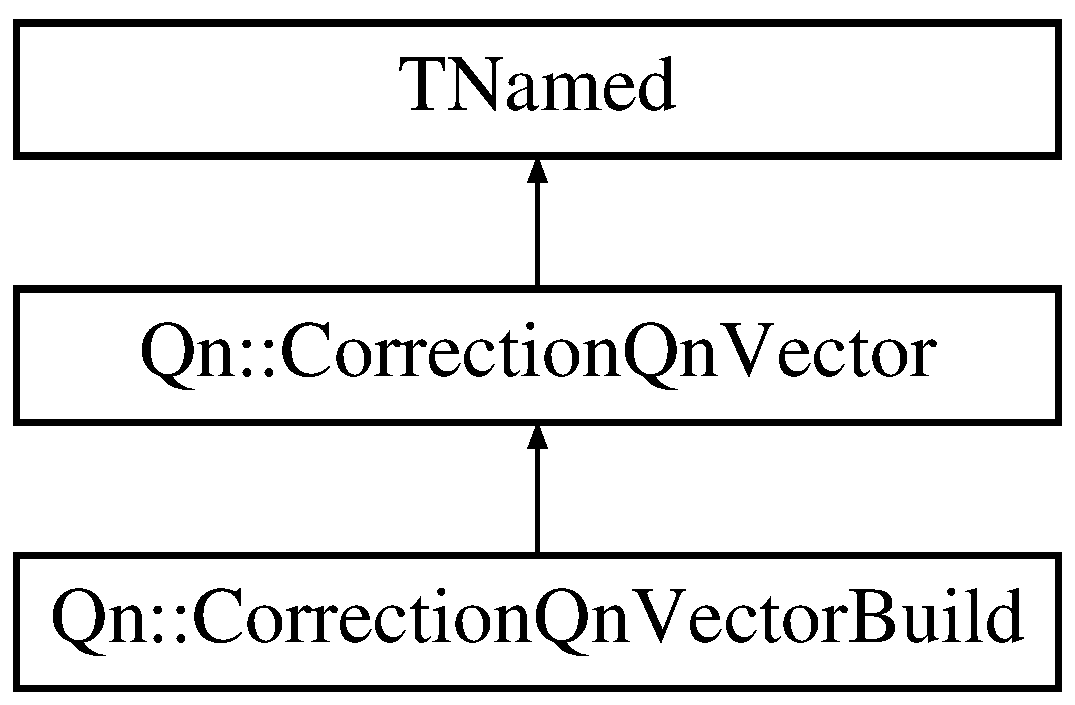
\includegraphics[height=3.000000cm]{classQn_1_1CorrectionQnVectorBuild}
\end{center}
\end{figure}
\subsection*{Public Member Functions}
\begin{DoxyCompactItemize}
\item 
\mbox{\Hypertarget{classQn_1_1CorrectionQnVectorBuild_a5c7b5d7cf75717b55b5ca94b3366523b}\label{classQn_1_1CorrectionQnVectorBuild_a5c7b5d7cf75717b55b5ca94b3366523b}} 
\mbox{\hyperlink{classQn_1_1CorrectionQnVectorBuild_a5c7b5d7cf75717b55b5ca94b3366523b}{Correction\+Qn\+Vector\+Build}} ()
\begin{DoxyCompactList}\small\item\em Default constructor. \end{DoxyCompactList}\item 
\mbox{\hyperlink{classQn_1_1CorrectionQnVectorBuild_a1f70d2bb07fe175a4aef27105f28429b}{Correction\+Qn\+Vector\+Build}} (const char $\ast$name, Int\+\_\+t n\+No\+Of\+Harmonics, Int\+\_\+t $\ast$harmonic\+Map=N\+U\+LL)
\item 
\mbox{\hyperlink{classQn_1_1CorrectionQnVectorBuild_a14c8e4495564ffd8250e4a90a9c4dae3}{Correction\+Qn\+Vector\+Build}} (const \mbox{\hyperlink{classQn_1_1CorrectionQnVector}{Correction\+Qn\+Vector}} \&Qn)
\item 
\mbox{\hyperlink{classQn_1_1CorrectionQnVectorBuild_ad75a0f924ed622ab07cbba8979917e91}{Correction\+Qn\+Vector\+Build}} (const \mbox{\hyperlink{classQn_1_1CorrectionQnVectorBuild}{Correction\+Qn\+Vector\+Build}} \&Qn)
\item 
\mbox{\Hypertarget{classQn_1_1CorrectionQnVectorBuild_ae4fea8e067dc5d8716ada23badb13261}\label{classQn_1_1CorrectionQnVectorBuild_ae4fea8e067dc5d8716ada23badb13261}} 
virtual \mbox{\hyperlink{classQn_1_1CorrectionQnVectorBuild_ae4fea8e067dc5d8716ada23badb13261}{$\sim$\+Correction\+Qn\+Vector\+Build}} ()
\begin{DoxyCompactList}\small\item\em Default destructor. \end{DoxyCompactList}\item 
virtual void \mbox{\hyperlink{classQn_1_1CorrectionQnVectorBuild_af4db1f1b7fc5650c39d3a3f232c184cf}{Set\+Qx}} (Int\+\_\+t harmonic, Float\+\_\+t qx)
\item 
virtual void \mbox{\hyperlink{classQn_1_1CorrectionQnVectorBuild_a1b9a7e2b0eafc48de05a2f90fcc51fb6}{Set\+Qy}} (Int\+\_\+t harmonic, Float\+\_\+t qy)
\item 
void \mbox{\hyperlink{classQn_1_1CorrectionQnVectorBuild_a07c8702ae5903f064a3fd53496f195cb}{Set}} (\mbox{\hyperlink{classQn_1_1CorrectionQnVectorBuild}{Correction\+Qn\+Vector\+Build}} $\ast$Qn)
\item 
void \mbox{\hyperlink{classQn_1_1CorrectionQnVectorBuild_aa7c654825f87b26452a1baeedcb0ac71}{Add}} (\mbox{\hyperlink{classQn_1_1CorrectionQnVectorBuild}{Correction\+Qn\+Vector\+Build}} $\ast$qvec)
\item 
void \mbox{\hyperlink{classQn_1_1CorrectionQnVectorBuild_abf29822fdbf4c7c05d6bc13961a4e5af}{Add}} (Double\+\_\+t phi, Double\+\_\+t weight=1.\+0)
\item 
void \mbox{\hyperlink{classQn_1_1CorrectionQnVectorBuild_a5f22254d0868abcb2f3a8db6f6e21416}{Check\+Quality}} ()
\item 
void \mbox{\hyperlink{classQn_1_1CorrectionQnVectorBuild_a2a16337a295cdf8674956432ad009d72}{Normalize}} (\mbox{\hyperlink{classQn_1_1CorrectionQnVector_a2998fe4babb716c57848c8c73b24a398}{Normalization}} method)
\item 
void \mbox{\hyperlink{classQn_1_1CorrectionQnVectorBuild_abe5a66d644a51087ddd3946bce0c58f5}{Normalize\+QoverM}} ()
\item 
void \mbox{\hyperlink{classQn_1_1CorrectionQnVectorBuild_a64644f0c2f52f98399db120028574fd3}{Normalize\+Qover\+Square\+Root\+OfM}} ()
\item 
\mbox{\Hypertarget{classQn_1_1CorrectionQnVectorBuild_a4a969142a64433fe57debb8ec5210329}\label{classQn_1_1CorrectionQnVectorBuild_a4a969142a64433fe57debb8ec5210329}} 
virtual void \mbox{\hyperlink{classQn_1_1CorrectionQnVectorBuild_a4a969142a64433fe57debb8ec5210329}{Reset}} ()
\begin{DoxyCompactList}\small\item\em Resets the Q vector values without touching the structure. \end{DoxyCompactList}\item 
virtual void \mbox{\hyperlink{classQn_1_1CorrectionQnVectorBuild_a8b767040ac4ae2472e8ce8f091b5ce88}{Print}} (Option\+\_\+t $\ast$) const
\end{DoxyCompactItemize}
\subsection*{Additional Inherited Members}


\subsection{Detailed Description}
Class that models and encapsulates a Q vector set while building it. 

When the Q vector is being built it needs extra support. This class provides such extra support.

\begin{DoxyAuthor}{Author}
Jaap Onderwaater \href{mailto:jacobus.onderwaater@cern.ch}{\tt jacobus.\+onderwaater@cern.\+ch}, G\+SI 

Ilya Selyuzhenkov \href{mailto:ilya.selyuzhenkov@gmail.com}{\tt ilya.\+selyuzhenkov@gmail.\+com}, G\+SI 

Víctor González \href{mailto:victor.gonzalez@cern.ch}{\tt victor.\+gonzalez@cern.\+ch}, U\+CM 
\end{DoxyAuthor}
\begin{DoxyDate}{Date}
Feb 02, 2016 
\end{DoxyDate}


\subsection{Constructor \& Destructor Documentation}
\mbox{\Hypertarget{classQn_1_1CorrectionQnVectorBuild_a1f70d2bb07fe175a4aef27105f28429b}\label{classQn_1_1CorrectionQnVectorBuild_a1f70d2bb07fe175a4aef27105f28429b}} 
\index{Qn\+::\+Correction\+Qn\+Vector\+Build@{Qn\+::\+Correction\+Qn\+Vector\+Build}!Correction\+Qn\+Vector\+Build@{Correction\+Qn\+Vector\+Build}}
\index{Correction\+Qn\+Vector\+Build@{Correction\+Qn\+Vector\+Build}!Qn\+::\+Correction\+Qn\+Vector\+Build@{Qn\+::\+Correction\+Qn\+Vector\+Build}}
\subsubsection{\texorpdfstring{Correction\+Qn\+Vector\+Build()}{CorrectionQnVectorBuild()}\hspace{0.1cm}{\footnotesize\ttfamily [1/3]}}
{\footnotesize\ttfamily Qn\+::\+Correction\+Qn\+Vector\+Build\+::\+Correction\+Qn\+Vector\+Build (\begin{DoxyParamCaption}\item[{const char $\ast$}]{name,  }\item[{Int\+\_\+t}]{n\+No\+Of\+Harmonics,  }\item[{Int\+\_\+t $\ast$}]{harmonic\+Map = {\ttfamily NULL} }\end{DoxyParamCaption})}

Normal constructor

Relays on its parent for almost everything


\begin{DoxyParams}{Parameters}
{\em name} & the name of the \mbox{\hyperlink{namespaceQn}{Qn}} vector. Identifies its origin \\
\hline
{\em n\+No\+Of\+Harmonics} & the desired number of harmonics \\
\hline
{\em harmonic\+Map} & ordered array with the external number of the harmonics \\
\hline
\end{DoxyParams}
\mbox{\Hypertarget{classQn_1_1CorrectionQnVectorBuild_a14c8e4495564ffd8250e4a90a9c4dae3}\label{classQn_1_1CorrectionQnVectorBuild_a14c8e4495564ffd8250e4a90a9c4dae3}} 
\index{Qn\+::\+Correction\+Qn\+Vector\+Build@{Qn\+::\+Correction\+Qn\+Vector\+Build}!Correction\+Qn\+Vector\+Build@{Correction\+Qn\+Vector\+Build}}
\index{Correction\+Qn\+Vector\+Build@{Correction\+Qn\+Vector\+Build}!Qn\+::\+Correction\+Qn\+Vector\+Build@{Qn\+::\+Correction\+Qn\+Vector\+Build}}
\subsubsection{\texorpdfstring{Correction\+Qn\+Vector\+Build()}{CorrectionQnVectorBuild()}\hspace{0.1cm}{\footnotesize\ttfamily [2/3]}}
{\footnotesize\ttfamily Qn\+::\+Correction\+Qn\+Vector\+Build\+::\+Correction\+Qn\+Vector\+Build (\begin{DoxyParamCaption}\item[{const \mbox{\hyperlink{classQn_1_1CorrectionQnVector}{Correction\+Qn\+Vector}} \&}]{Qn }\end{DoxyParamCaption})}

Copy constructor from a Q vector 
\begin{DoxyParams}{Parameters}
{\em \mbox{\hyperlink{namespaceQn}{Qn}}} & the Q vector build object to copy after construction \\
\hline
\end{DoxyParams}
\mbox{\Hypertarget{classQn_1_1CorrectionQnVectorBuild_ad75a0f924ed622ab07cbba8979917e91}\label{classQn_1_1CorrectionQnVectorBuild_ad75a0f924ed622ab07cbba8979917e91}} 
\index{Qn\+::\+Correction\+Qn\+Vector\+Build@{Qn\+::\+Correction\+Qn\+Vector\+Build}!Correction\+Qn\+Vector\+Build@{Correction\+Qn\+Vector\+Build}}
\index{Correction\+Qn\+Vector\+Build@{Correction\+Qn\+Vector\+Build}!Qn\+::\+Correction\+Qn\+Vector\+Build@{Qn\+::\+Correction\+Qn\+Vector\+Build}}
\subsubsection{\texorpdfstring{Correction\+Qn\+Vector\+Build()}{CorrectionQnVectorBuild()}\hspace{0.1cm}{\footnotesize\ttfamily [3/3]}}
{\footnotesize\ttfamily Qn\+::\+Correction\+Qn\+Vector\+Build\+::\+Correction\+Qn\+Vector\+Build (\begin{DoxyParamCaption}\item[{const \mbox{\hyperlink{classQn_1_1CorrectionQnVectorBuild}{Correction\+Qn\+Vector\+Build}} \&}]{Qn }\end{DoxyParamCaption})}

Copy constructor 
\begin{DoxyParams}{Parameters}
{\em \mbox{\hyperlink{namespaceQn}{Qn}}} & the Q vector build object to copy after construction \\
\hline
\end{DoxyParams}


\subsection{Member Function Documentation}
\mbox{\Hypertarget{classQn_1_1CorrectionQnVectorBuild_aa7c654825f87b26452a1baeedcb0ac71}\label{classQn_1_1CorrectionQnVectorBuild_aa7c654825f87b26452a1baeedcb0ac71}} 
\index{Qn\+::\+Correction\+Qn\+Vector\+Build@{Qn\+::\+Correction\+Qn\+Vector\+Build}!Add@{Add}}
\index{Add@{Add}!Qn\+::\+Correction\+Qn\+Vector\+Build@{Qn\+::\+Correction\+Qn\+Vector\+Build}}
\subsubsection{\texorpdfstring{Add()}{Add()}\hspace{0.1cm}{\footnotesize\ttfamily [1/2]}}
{\footnotesize\ttfamily void Qn\+::\+Correction\+Qn\+Vector\+Build\+::\+Add (\begin{DoxyParamCaption}\item[{\mbox{\hyperlink{classQn_1_1CorrectionQnVectorBuild}{Correction\+Qn\+Vector\+Build}} $\ast$}]{Qn }\end{DoxyParamCaption})}

Adds a build Q vector

The possibility of a different set of harmonics for both build Q vectors is considered. A run time error is raised if they do not match. 
\begin{DoxyParams}{Parameters}
{\em \mbox{\hyperlink{namespaceQn}{Qn}}} & the build Q vector to add \\
\hline
\end{DoxyParams}
\mbox{\Hypertarget{classQn_1_1CorrectionQnVectorBuild_abf29822fdbf4c7c05d6bc13961a4e5af}\label{classQn_1_1CorrectionQnVectorBuild_abf29822fdbf4c7c05d6bc13961a4e5af}} 
\index{Qn\+::\+Correction\+Qn\+Vector\+Build@{Qn\+::\+Correction\+Qn\+Vector\+Build}!Add@{Add}}
\index{Add@{Add}!Qn\+::\+Correction\+Qn\+Vector\+Build@{Qn\+::\+Correction\+Qn\+Vector\+Build}}
\subsubsection{\texorpdfstring{Add()}{Add()}\hspace{0.1cm}{\footnotesize\ttfamily [2/2]}}
{\footnotesize\ttfamily void Qn\+::\+Correction\+Qn\+Vector\+Build\+::\+Add (\begin{DoxyParamCaption}\item[{Double\+\_\+t}]{phi,  }\item[{Double\+\_\+t}]{weight = {\ttfamily 1.0} }\end{DoxyParamCaption})\hspace{0.3cm}{\ttfamily [inline]}}

Adds a contribution to the build Q vector A check for weight significant value is made. Not passing it ignores the contribution. The process of incorporating contributions takes into account the harmonic multiplier 
\begin{DoxyParams}{Parameters}
{\em phi} & azimuthal angle contribution \\
\hline
{\em weight} & the weight of the contribution \\
\hline
\end{DoxyParams}
\mbox{\Hypertarget{classQn_1_1CorrectionQnVectorBuild_a5f22254d0868abcb2f3a8db6f6e21416}\label{classQn_1_1CorrectionQnVectorBuild_a5f22254d0868abcb2f3a8db6f6e21416}} 
\index{Qn\+::\+Correction\+Qn\+Vector\+Build@{Qn\+::\+Correction\+Qn\+Vector\+Build}!Check\+Quality@{Check\+Quality}}
\index{Check\+Quality@{Check\+Quality}!Qn\+::\+Correction\+Qn\+Vector\+Build@{Qn\+::\+Correction\+Qn\+Vector\+Build}}
\subsubsection{\texorpdfstring{Check\+Quality()}{CheckQuality()}}
{\footnotesize\ttfamily void Qn\+::\+Correction\+Qn\+Vector\+Build\+::\+Check\+Quality (\begin{DoxyParamCaption}{ }\end{DoxyParamCaption})\hspace{0.3cm}{\ttfamily [inline]}}

Check the quality of the constructed \mbox{\hyperlink{namespaceQn}{Qn}} vector Current criteria is number of contributors should be at least one. If so happen, sets the good quality flag. \mbox{\Hypertarget{classQn_1_1CorrectionQnVectorBuild_a2a16337a295cdf8674956432ad009d72}\label{classQn_1_1CorrectionQnVectorBuild_a2a16337a295cdf8674956432ad009d72}} 
\index{Qn\+::\+Correction\+Qn\+Vector\+Build@{Qn\+::\+Correction\+Qn\+Vector\+Build}!Normalize@{Normalize}}
\index{Normalize@{Normalize}!Qn\+::\+Correction\+Qn\+Vector\+Build@{Qn\+::\+Correction\+Qn\+Vector\+Build}}
\subsubsection{\texorpdfstring{Normalize()}{Normalize()}}
{\footnotesize\ttfamily void Qn\+::\+Correction\+Qn\+Vector\+Build\+::\+Normalize (\begin{DoxyParamCaption}\item[{\mbox{\hyperlink{classQn_1_1CorrectionQnVector_a2998fe4babb716c57848c8c73b24a398}{Normalization}}}]{method }\end{DoxyParamCaption})\hspace{0.3cm}{\ttfamily [inline]}}

Calibrates the Q vector according to the method passed 
\begin{DoxyParams}{Parameters}
{\em method} & the method of calibration \\
\hline
\end{DoxyParams}
\mbox{\Hypertarget{classQn_1_1CorrectionQnVectorBuild_abe5a66d644a51087ddd3946bce0c58f5}\label{classQn_1_1CorrectionQnVectorBuild_abe5a66d644a51087ddd3946bce0c58f5}} 
\index{Qn\+::\+Correction\+Qn\+Vector\+Build@{Qn\+::\+Correction\+Qn\+Vector\+Build}!Normalize\+QoverM@{Normalize\+QoverM}}
\index{Normalize\+QoverM@{Normalize\+QoverM}!Qn\+::\+Correction\+Qn\+Vector\+Build@{Qn\+::\+Correction\+Qn\+Vector\+Build}}
\subsubsection{\texorpdfstring{Normalize\+Qover\+M()}{NormalizeQoverM()}}
{\footnotesize\ttfamily void Qn\+::\+Correction\+Qn\+Vector\+Build\+::\+Normalize\+QoverM (\begin{DoxyParamCaption}{ }\end{DoxyParamCaption})}

Normalizes the build Q vector for the whole harmonics set

Normalizes the build Q vector as $ Qn = \frac{Qn}{M} $. A check for significant value is made. Not passing it does set the Q vector quality as bad \mbox{\Hypertarget{classQn_1_1CorrectionQnVectorBuild_a64644f0c2f52f98399db120028574fd3}\label{classQn_1_1CorrectionQnVectorBuild_a64644f0c2f52f98399db120028574fd3}} 
\index{Qn\+::\+Correction\+Qn\+Vector\+Build@{Qn\+::\+Correction\+Qn\+Vector\+Build}!Normalize\+Qover\+Square\+Root\+OfM@{Normalize\+Qover\+Square\+Root\+OfM}}
\index{Normalize\+Qover\+Square\+Root\+OfM@{Normalize\+Qover\+Square\+Root\+OfM}!Qn\+::\+Correction\+Qn\+Vector\+Build@{Qn\+::\+Correction\+Qn\+Vector\+Build}}
\subsubsection{\texorpdfstring{Normalize\+Qover\+Square\+Root\+Of\+M()}{NormalizeQoverSquareRootOfM()}}
{\footnotesize\ttfamily void Qn\+::\+Correction\+Qn\+Vector\+Build\+::\+Normalize\+Qover\+Square\+Root\+OfM (\begin{DoxyParamCaption}{ }\end{DoxyParamCaption})}

Normalizes the build Q vector for the whole harmonics set

Normalizes the build Q vector as $ Qn = \frac{Qn}{\sqrt{M}} $. A check for significant value is made. Not passing it does set the Q vector quality as bad \mbox{\Hypertarget{classQn_1_1CorrectionQnVectorBuild_a8b767040ac4ae2472e8ce8f091b5ce88}\label{classQn_1_1CorrectionQnVectorBuild_a8b767040ac4ae2472e8ce8f091b5ce88}} 
\index{Qn\+::\+Correction\+Qn\+Vector\+Build@{Qn\+::\+Correction\+Qn\+Vector\+Build}!Print@{Print}}
\index{Print@{Print}!Qn\+::\+Correction\+Qn\+Vector\+Build@{Qn\+::\+Correction\+Qn\+Vector\+Build}}
\subsubsection{\texorpdfstring{Print()}{Print()}}
{\footnotesize\ttfamily void Qn\+::\+Correction\+Qn\+Vector\+Build\+::\+Print (\begin{DoxyParamCaption}\item[{Option\+\_\+t $\ast$}]{ }\end{DoxyParamCaption}) const\hspace{0.3cm}{\ttfamily [virtual]}}

Print the \mbox{\hyperlink{namespaceQn}{Qn}} vector in a readable shape 

Reimplemented from \mbox{\hyperlink{classQn_1_1CorrectionQnVector_a859e8ffe20c7a607f67bb95f8c85b9e9}{Qn\+::\+Correction\+Qn\+Vector}}.

\mbox{\Hypertarget{classQn_1_1CorrectionQnVectorBuild_a07c8702ae5903f064a3fd53496f195cb}\label{classQn_1_1CorrectionQnVectorBuild_a07c8702ae5903f064a3fd53496f195cb}} 
\index{Qn\+::\+Correction\+Qn\+Vector\+Build@{Qn\+::\+Correction\+Qn\+Vector\+Build}!Set@{Set}}
\index{Set@{Set}!Qn\+::\+Correction\+Qn\+Vector\+Build@{Qn\+::\+Correction\+Qn\+Vector\+Build}}
\subsubsection{\texorpdfstring{Set()}{Set()}}
{\footnotesize\ttfamily void Qn\+::\+Correction\+Qn\+Vector\+Build\+::\+Set (\begin{DoxyParamCaption}\item[{\mbox{\hyperlink{classQn_1_1CorrectionQnVectorBuild}{Correction\+Qn\+Vector\+Build}} $\ast$}]{Qn }\end{DoxyParamCaption})}

Copy member function

The passed Q vector is copied within the current object 
\begin{DoxyParams}{Parameters}
{\em \mbox{\hyperlink{namespaceQn}{Qn}}} & pointer to the Q vector to be copied \\
\hline
\end{DoxyParams}
\mbox{\Hypertarget{classQn_1_1CorrectionQnVectorBuild_af4db1f1b7fc5650c39d3a3f232c184cf}\label{classQn_1_1CorrectionQnVectorBuild_af4db1f1b7fc5650c39d3a3f232c184cf}} 
\index{Qn\+::\+Correction\+Qn\+Vector\+Build@{Qn\+::\+Correction\+Qn\+Vector\+Build}!Set\+Qx@{Set\+Qx}}
\index{Set\+Qx@{Set\+Qx}!Qn\+::\+Correction\+Qn\+Vector\+Build@{Qn\+::\+Correction\+Qn\+Vector\+Build}}
\subsubsection{\texorpdfstring{Set\+Qx()}{SetQx()}}
{\footnotesize\ttfamily void Qn\+::\+Correction\+Qn\+Vector\+Build\+::\+Set\+Qx (\begin{DoxyParamCaption}\item[{Int\+\_\+t}]{harmonic,  }\item[{Float\+\_\+t}]{qx }\end{DoxyParamCaption})\hspace{0.3cm}{\ttfamily [virtual]}}

Sets the X component for the considered harmonic

It should not be used. Runtime error indication. 

Reimplemented from \mbox{\hyperlink{classQn_1_1CorrectionQnVector_a6de477e3cecce7c5f5b9212ecbafea59}{Qn\+::\+Correction\+Qn\+Vector}}.

\mbox{\Hypertarget{classQn_1_1CorrectionQnVectorBuild_a1b9a7e2b0eafc48de05a2f90fcc51fb6}\label{classQn_1_1CorrectionQnVectorBuild_a1b9a7e2b0eafc48de05a2f90fcc51fb6}} 
\index{Qn\+::\+Correction\+Qn\+Vector\+Build@{Qn\+::\+Correction\+Qn\+Vector\+Build}!Set\+Qy@{Set\+Qy}}
\index{Set\+Qy@{Set\+Qy}!Qn\+::\+Correction\+Qn\+Vector\+Build@{Qn\+::\+Correction\+Qn\+Vector\+Build}}
\subsubsection{\texorpdfstring{Set\+Qy()}{SetQy()}}
{\footnotesize\ttfamily void Qn\+::\+Correction\+Qn\+Vector\+Build\+::\+Set\+Qy (\begin{DoxyParamCaption}\item[{Int\+\_\+t}]{harmonic,  }\item[{Float\+\_\+t}]{qy }\end{DoxyParamCaption})\hspace{0.3cm}{\ttfamily [virtual]}}

Sets the Y component for the considered harmonic

It should not be used. Runtime error indication. 

Reimplemented from \mbox{\hyperlink{classQn_1_1CorrectionQnVector_af0ac581e943fe88b0a94838c670f2c4d}{Qn\+::\+Correction\+Qn\+Vector}}.



The documentation for this class was generated from the following files\+:\begin{DoxyCompactItemize}
\item 
D\+T\+\_\+\+Flow/\+Qn\+Corrections/include/\mbox{\hyperlink{CorrectionQnVectorBuild_8h}{Correction\+Qn\+Vector\+Build.\+h}}\item 
D\+T\+\_\+\+Flow/\+Qn\+Corrections/Correction\+Qn\+Vector\+Build.\+cpp\end{DoxyCompactItemize}

\hypertarget{classQn_1_1CorrectionsSetOnInputData}{}\section{Qn\+:\+:Corrections\+Set\+On\+Input\+Data Class Reference}
\label{classQn_1_1CorrectionsSetOnInputData}\index{Qn\+::\+Corrections\+Set\+On\+Input\+Data@{Qn\+::\+Corrections\+Set\+On\+Input\+Data}}
Inheritance diagram for Qn\+:\+:Corrections\+Set\+On\+Input\+Data\+:\begin{figure}[H]
\begin{center}
\leavevmode
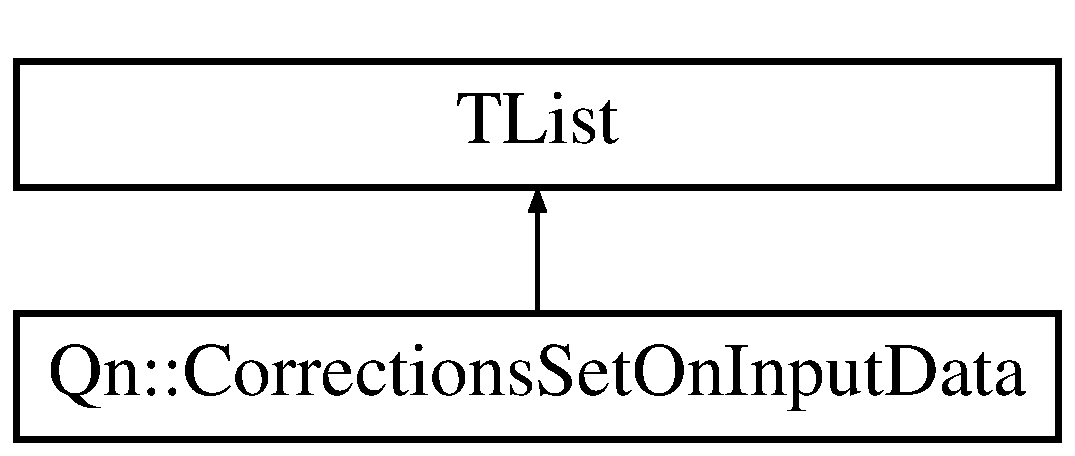
\includegraphics[height=2.000000cm]{classQn_1_1CorrectionsSetOnInputData}
\end{center}
\end{figure}
\subsection*{Public Member Functions}
\begin{DoxyCompactItemize}
\item 
\mbox{\Hypertarget{classQn_1_1CorrectionsSetOnInputData_a38a9a90d6071c5af09a4ed6a30c0bb0f}\label{classQn_1_1CorrectionsSetOnInputData_a38a9a90d6071c5af09a4ed6a30c0bb0f}} 
\mbox{\hyperlink{classQn_1_1CorrectionsSetOnInputData_a38a9a90d6071c5af09a4ed6a30c0bb0f}{Corrections\+Set\+On\+Input\+Data}} ()
\begin{DoxyCompactList}\small\item\em Default constructor. \end{DoxyCompactList}\item 
\mbox{\Hypertarget{classQn_1_1CorrectionsSetOnInputData_a29c9c3d13112653a7e163d3aa7615c6c}\label{classQn_1_1CorrectionsSetOnInputData_a29c9c3d13112653a7e163d3aa7615c6c}} 
virtual \mbox{\hyperlink{classQn_1_1CorrectionsSetOnInputData_a29c9c3d13112653a7e163d3aa7615c6c}{$\sim$\+Corrections\+Set\+On\+Input\+Data}} ()
\begin{DoxyCompactList}\small\item\em Default destructor. \end{DoxyCompactList}\item 
virtual \mbox{\hyperlink{classQn_1_1CorrectionOnInputData}{Correction\+On\+Input\+Data}} $\ast$ \mbox{\hyperlink{classQn_1_1CorrectionsSetOnInputData_a7d23f9a8c9f61fbe94b2b2257b599c06}{At}} (Int\+\_\+t i) const
\item 
void \mbox{\hyperlink{classQn_1_1CorrectionsSetOnInputData_ae7bc47aa87b78daca76889e45952766a}{Add\+Correction}} (\mbox{\hyperlink{classQn_1_1CorrectionOnInputData}{Correction\+On\+Input\+Data}} $\ast$correction)
\item 
void \mbox{\hyperlink{classQn_1_1CorrectionsSetOnInputData_af1489e16bd450a64cbb33654e7559568}{Fill\+Overall\+Corrections\+List}} (T\+List $\ast$correctionlist) const
\end{DoxyCompactItemize}


\subsection{Member Function Documentation}
\mbox{\Hypertarget{classQn_1_1CorrectionsSetOnInputData_ae7bc47aa87b78daca76889e45952766a}\label{classQn_1_1CorrectionsSetOnInputData_ae7bc47aa87b78daca76889e45952766a}} 
\index{Qn\+::\+Corrections\+Set\+On\+Input\+Data@{Qn\+::\+Corrections\+Set\+On\+Input\+Data}!Add\+Correction@{Add\+Correction}}
\index{Add\+Correction@{Add\+Correction}!Qn\+::\+Corrections\+Set\+On\+Input\+Data@{Qn\+::\+Corrections\+Set\+On\+Input\+Data}}
\subsubsection{\texorpdfstring{Add\+Correction()}{AddCorrection()}}
{\footnotesize\ttfamily void Qn\+::\+Corrections\+Set\+On\+Input\+Data\+::\+Add\+Correction (\begin{DoxyParamCaption}\item[{\mbox{\hyperlink{classQn_1_1CorrectionOnInputData}{Correction\+On\+Input\+Data}} $\ast$}]{correction }\end{DoxyParamCaption})}

Adds a new correction to the set.

The correction is incorporated in its proper place according to its key \mbox{\Hypertarget{classQn_1_1CorrectionsSetOnInputData_a7d23f9a8c9f61fbe94b2b2257b599c06}\label{classQn_1_1CorrectionsSetOnInputData_a7d23f9a8c9f61fbe94b2b2257b599c06}} 
\index{Qn\+::\+Corrections\+Set\+On\+Input\+Data@{Qn\+::\+Corrections\+Set\+On\+Input\+Data}!At@{At}}
\index{At@{At}!Qn\+::\+Corrections\+Set\+On\+Input\+Data@{Qn\+::\+Corrections\+Set\+On\+Input\+Data}}
\subsubsection{\texorpdfstring{At()}{At()}}
{\footnotesize\ttfamily virtual \mbox{\hyperlink{classQn_1_1CorrectionOnInputData}{Correction\+On\+Input\+Data}}$\ast$ Qn\+::\+Corrections\+Set\+On\+Input\+Data\+::\+At (\begin{DoxyParamCaption}\item[{Int\+\_\+t}]{i }\end{DoxyParamCaption}) const\hspace{0.3cm}{\ttfamily [inline]}, {\ttfamily [virtual]}}

Access the correction step at the passed position 
\begin{DoxyParams}{Parameters}
{\em i} & position in the list (starting at zero) \\
\hline
\end{DoxyParams}
\begin{DoxyReturn}{Returns}
the correction step object a position i 
\end{DoxyReturn}
\mbox{\Hypertarget{classQn_1_1CorrectionsSetOnInputData_af1489e16bd450a64cbb33654e7559568}\label{classQn_1_1CorrectionsSetOnInputData_af1489e16bd450a64cbb33654e7559568}} 
\index{Qn\+::\+Corrections\+Set\+On\+Input\+Data@{Qn\+::\+Corrections\+Set\+On\+Input\+Data}!Fill\+Overall\+Corrections\+List@{Fill\+Overall\+Corrections\+List}}
\index{Fill\+Overall\+Corrections\+List@{Fill\+Overall\+Corrections\+List}!Qn\+::\+Corrections\+Set\+On\+Input\+Data@{Qn\+::\+Corrections\+Set\+On\+Input\+Data}}
\subsubsection{\texorpdfstring{Fill\+Overall\+Corrections\+List()}{FillOverallCorrectionsList()}}
{\footnotesize\ttfamily void Qn\+::\+Corrections\+Set\+On\+Input\+Data\+::\+Fill\+Overall\+Corrections\+List (\begin{DoxyParamCaption}\item[{T\+List $\ast$}]{correctionlist }\end{DoxyParamCaption}) const}

Fill the global list of correction steps 
\begin{DoxyParams}{Parameters}
{\em correctionlist} & (partial) global list of corrections ordered by correction key \\
\hline
\end{DoxyParams}


The documentation for this class was generated from the following files\+:\begin{DoxyCompactItemize}
\item 
D\+T\+\_\+\+Flow/\+Qn\+Corrections/include/Corrections\+Set\+On\+Input\+Data.\+h\item 
D\+T\+\_\+\+Flow/\+Qn\+Corrections/Corrections\+Set\+On\+Input\+Data.\+cpp\end{DoxyCompactItemize}

\hypertarget{classQn_1_1CorrectionsSetOnQvector}{}\section{Qn\+:\+:Corrections\+Set\+On\+Qvector Class Reference}
\label{classQn_1_1CorrectionsSetOnQvector}\index{Qn\+::\+Corrections\+Set\+On\+Qvector@{Qn\+::\+Corrections\+Set\+On\+Qvector}}
Inheritance diagram for Qn\+:\+:Corrections\+Set\+On\+Qvector\+:\begin{figure}[H]
\begin{center}
\leavevmode
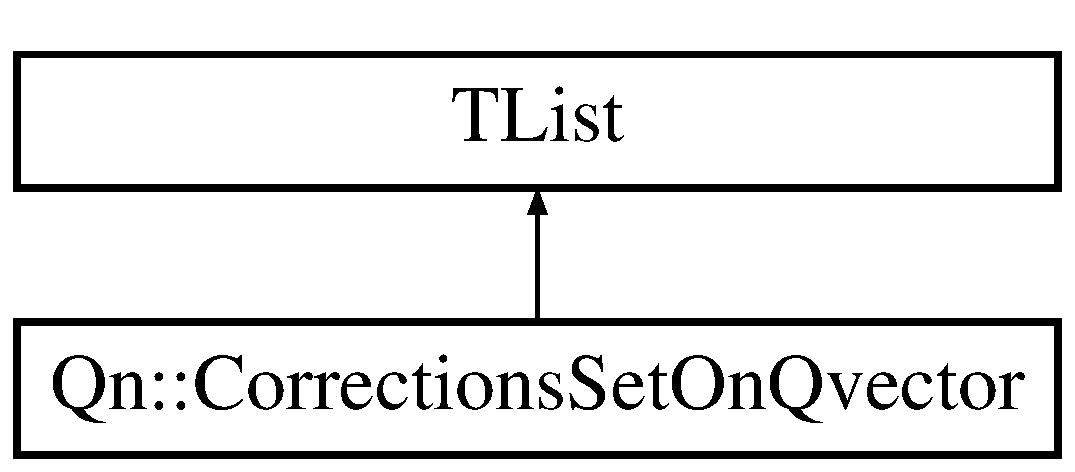
\includegraphics[height=2.000000cm]{classQn_1_1CorrectionsSetOnQvector}
\end{center}
\end{figure}
\subsection*{Public Member Functions}
\begin{DoxyCompactItemize}
\item 
\mbox{\Hypertarget{classQn_1_1CorrectionsSetOnQvector_a20e825161ee60dd975b854a389d31c75}\label{classQn_1_1CorrectionsSetOnQvector_a20e825161ee60dd975b854a389d31c75}} 
\mbox{\hyperlink{classQn_1_1CorrectionsSetOnQvector_a20e825161ee60dd975b854a389d31c75}{Corrections\+Set\+On\+Qvector}} ()
\begin{DoxyCompactList}\small\item\em Default constructor. \end{DoxyCompactList}\item 
\mbox{\Hypertarget{classQn_1_1CorrectionsSetOnQvector_af0fdb3a7fd8ce387a253b187e3cb5b69}\label{classQn_1_1CorrectionsSetOnQvector_af0fdb3a7fd8ce387a253b187e3cb5b69}} 
virtual \mbox{\hyperlink{classQn_1_1CorrectionsSetOnQvector_af0fdb3a7fd8ce387a253b187e3cb5b69}{$\sim$\+Corrections\+Set\+On\+Qvector}} ()
\begin{DoxyCompactList}\small\item\em Default destructor. \end{DoxyCompactList}\item 
virtual \mbox{\hyperlink{classQn_1_1CorrectionOnQvector}{Correction\+On\+Qvector}} $\ast$ \mbox{\hyperlink{classQn_1_1CorrectionsSetOnQvector_aada04695d30c1c736be32f7ef47df39b}{At}} (Int\+\_\+t i) const
\item 
void \mbox{\hyperlink{classQn_1_1CorrectionsSetOnQvector_abad0a3b5ab01df6e8b8392353cbdbbbe}{Add\+Correction}} (\mbox{\hyperlink{classQn_1_1CorrectionOnQvector}{Correction\+On\+Qvector}} $\ast$correction)
\item 
void \mbox{\hyperlink{classQn_1_1CorrectionsSetOnQvector_a30278af9b844840208baad107e68ea69}{Fill\+Overall\+Corrections\+List}} (T\+List $\ast$correctionlist) const
\item 
const \mbox{\hyperlink{classQn_1_1CorrectionOnQvector}{Correction\+On\+Qvector}} $\ast$ \mbox{\hyperlink{classQn_1_1CorrectionsSetOnQvector_ade101be45b400b1b34f253eed75ccf9f}{Get\+Previous}} (const \mbox{\hyperlink{classQn_1_1CorrectionOnQvector}{Correction\+On\+Qvector}} $\ast$correction) const
\item 
Bool\+\_\+t \mbox{\hyperlink{classQn_1_1CorrectionsSetOnQvector_a5b434f22965975e0131ec0938afcf665}{Is\+Correction\+Step\+Being\+Applied}} (const char $\ast$name) const
\end{DoxyCompactItemize}


\subsection{Member Function Documentation}
\mbox{\Hypertarget{classQn_1_1CorrectionsSetOnQvector_abad0a3b5ab01df6e8b8392353cbdbbbe}\label{classQn_1_1CorrectionsSetOnQvector_abad0a3b5ab01df6e8b8392353cbdbbbe}} 
\index{Qn\+::\+Corrections\+Set\+On\+Qvector@{Qn\+::\+Corrections\+Set\+On\+Qvector}!Add\+Correction@{Add\+Correction}}
\index{Add\+Correction@{Add\+Correction}!Qn\+::\+Corrections\+Set\+On\+Qvector@{Qn\+::\+Corrections\+Set\+On\+Qvector}}
\subsubsection{\texorpdfstring{Add\+Correction()}{AddCorrection()}}
{\footnotesize\ttfamily void Qn\+::\+Corrections\+Set\+On\+Qvector\+::\+Add\+Correction (\begin{DoxyParamCaption}\item[{\mbox{\hyperlink{classQn_1_1CorrectionOnQvector}{Correction\+On\+Qvector}} $\ast$}]{correction }\end{DoxyParamCaption})}

Adds a new correction to the set.

The correction is incorporated in its proper place according to its key \mbox{\Hypertarget{classQn_1_1CorrectionsSetOnQvector_aada04695d30c1c736be32f7ef47df39b}\label{classQn_1_1CorrectionsSetOnQvector_aada04695d30c1c736be32f7ef47df39b}} 
\index{Qn\+::\+Corrections\+Set\+On\+Qvector@{Qn\+::\+Corrections\+Set\+On\+Qvector}!At@{At}}
\index{At@{At}!Qn\+::\+Corrections\+Set\+On\+Qvector@{Qn\+::\+Corrections\+Set\+On\+Qvector}}
\subsubsection{\texorpdfstring{At()}{At()}}
{\footnotesize\ttfamily virtual \mbox{\hyperlink{classQn_1_1CorrectionOnQvector}{Correction\+On\+Qvector}}$\ast$ Qn\+::\+Corrections\+Set\+On\+Qvector\+::\+At (\begin{DoxyParamCaption}\item[{Int\+\_\+t}]{i }\end{DoxyParamCaption}) const\hspace{0.3cm}{\ttfamily [inline]}, {\ttfamily [virtual]}}

Access the correction step at the passed position 
\begin{DoxyParams}{Parameters}
{\em i} & position in the list (starting at zero) \\
\hline
\end{DoxyParams}
\begin{DoxyReturn}{Returns}
the correction step object a position i 
\end{DoxyReturn}
\mbox{\Hypertarget{classQn_1_1CorrectionsSetOnQvector_a30278af9b844840208baad107e68ea69}\label{classQn_1_1CorrectionsSetOnQvector_a30278af9b844840208baad107e68ea69}} 
\index{Qn\+::\+Corrections\+Set\+On\+Qvector@{Qn\+::\+Corrections\+Set\+On\+Qvector}!Fill\+Overall\+Corrections\+List@{Fill\+Overall\+Corrections\+List}}
\index{Fill\+Overall\+Corrections\+List@{Fill\+Overall\+Corrections\+List}!Qn\+::\+Corrections\+Set\+On\+Qvector@{Qn\+::\+Corrections\+Set\+On\+Qvector}}
\subsubsection{\texorpdfstring{Fill\+Overall\+Corrections\+List()}{FillOverallCorrectionsList()}}
{\footnotesize\ttfamily void Qn\+::\+Corrections\+Set\+On\+Qvector\+::\+Fill\+Overall\+Corrections\+List (\begin{DoxyParamCaption}\item[{T\+List $\ast$}]{correctionlist }\end{DoxyParamCaption}) const}

Fill the global list of correction steps 
\begin{DoxyParams}{Parameters}
{\em correctionlist} & (partial) global list of corrections ordered by correction key \\
\hline
\end{DoxyParams}
\mbox{\Hypertarget{classQn_1_1CorrectionsSetOnQvector_ade101be45b400b1b34f253eed75ccf9f}\label{classQn_1_1CorrectionsSetOnQvector_ade101be45b400b1b34f253eed75ccf9f}} 
\index{Qn\+::\+Corrections\+Set\+On\+Qvector@{Qn\+::\+Corrections\+Set\+On\+Qvector}!Get\+Previous@{Get\+Previous}}
\index{Get\+Previous@{Get\+Previous}!Qn\+::\+Corrections\+Set\+On\+Qvector@{Qn\+::\+Corrections\+Set\+On\+Qvector}}
\subsubsection{\texorpdfstring{Get\+Previous()}{GetPrevious()}}
{\footnotesize\ttfamily const \mbox{\hyperlink{classQn_1_1CorrectionOnQvector}{Correction\+On\+Qvector}} $\ast$ Qn\+::\+Corrections\+Set\+On\+Qvector\+::\+Get\+Previous (\begin{DoxyParamCaption}\item[{const \mbox{\hyperlink{classQn_1_1CorrectionOnQvector}{Correction\+On\+Qvector}} $\ast$}]{correction }\end{DoxyParamCaption}) const}

Gets the correction on \mbox{\hyperlink{namespaceQn}{Qn}} vector previous to the one passed as argument 
\begin{DoxyParams}{Parameters}
{\em correction} & the correction to find the previous one \\
\hline
\end{DoxyParams}
\begin{DoxyReturn}{Returns}
the previous correction, N\+U\+LL if none 
\end{DoxyReturn}
\mbox{\Hypertarget{classQn_1_1CorrectionsSetOnQvector_a5b434f22965975e0131ec0938afcf665}\label{classQn_1_1CorrectionsSetOnQvector_a5b434f22965975e0131ec0938afcf665}} 
\index{Qn\+::\+Corrections\+Set\+On\+Qvector@{Qn\+::\+Corrections\+Set\+On\+Qvector}!Is\+Correction\+Step\+Being\+Applied@{Is\+Correction\+Step\+Being\+Applied}}
\index{Is\+Correction\+Step\+Being\+Applied@{Is\+Correction\+Step\+Being\+Applied}!Qn\+::\+Corrections\+Set\+On\+Qvector@{Qn\+::\+Corrections\+Set\+On\+Qvector}}
\subsubsection{\texorpdfstring{Is\+Correction\+Step\+Being\+Applied()}{IsCorrectionStepBeingApplied()}}
{\footnotesize\ttfamily Bool\+\_\+t Qn\+::\+Corrections\+Set\+On\+Qvector\+::\+Is\+Correction\+Step\+Being\+Applied (\begin{DoxyParamCaption}\item[{const char $\ast$}]{step }\end{DoxyParamCaption}) const}

Check if a concrete correction step is bein applied on this detector configuration It is not enough having the correction step configured or collecting data. To get an affirmative answer the correction step must be being applied. Transfer the order to each of the \mbox{\hyperlink{namespaceQn}{Qn}} correction steps. 
\begin{DoxyParams}{Parameters}
{\em step} & the name of the correction step \\
\hline
\end{DoxyParams}
\begin{DoxyReturn}{Returns}
T\+R\+UE if the correction step is being applied 
\end{DoxyReturn}


The documentation for this class was generated from the following files\+:\begin{DoxyCompactItemize}
\item 
D\+T\+\_\+\+Flow/\+Qn\+Corrections/include/Corrections\+Set\+On\+Qvector.\+h\item 
D\+T\+\_\+\+Flow/\+Qn\+Corrections/Corrections\+Set\+On\+Qvector.\+cpp\end{DoxyCompactItemize}

\hypertarget{classQn_1_1CorrectionStepBase}{}\section{Qn\+:\+:Correction\+Step\+Base Class Reference}
\label{classQn_1_1CorrectionStepBase}\index{Qn\+::\+Correction\+Step\+Base@{Qn\+::\+Correction\+Step\+Base}}
Inheritance diagram for Qn\+:\+:Correction\+Step\+Base\+:\begin{figure}[H]
\begin{center}
\leavevmode
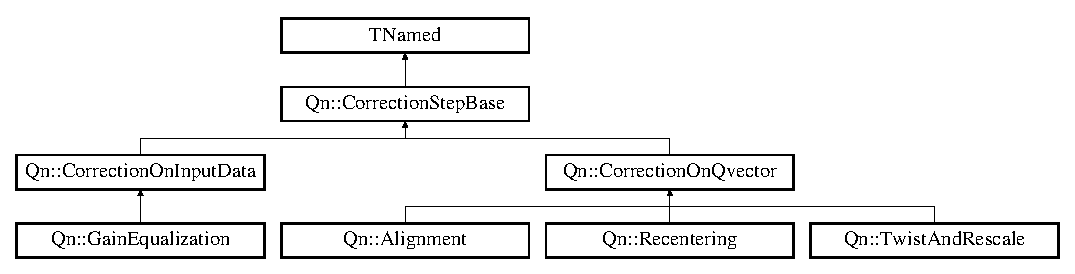
\includegraphics[height=3.236994cm]{classQn_1_1CorrectionStepBase}
\end{center}
\end{figure}
\subsection*{Public Types}
\begin{DoxyCompactItemize}
\item 
enum \mbox{\hyperlink{classQn_1_1CorrectionStepBase_a95ce2afbf677e1303b632df2399c8620}{Qn\+Correction\+Step\+Status}} \{ \mbox{\hyperlink{classQn_1_1CorrectionStepBase_a95ce2afbf677e1303b632df2399c8620abe46b97678dbe8da01af1dd4975f699b}{Q\+C\+O\+R\+R\+S\+T\+E\+P\+\_\+calibration}}, 
\mbox{\hyperlink{classQn_1_1CorrectionStepBase_a95ce2afbf677e1303b632df2399c8620a885ea58428f7a1d330f24a5a958e0250}{Q\+C\+O\+R\+R\+S\+T\+E\+P\+\_\+apply}}, 
\mbox{\hyperlink{classQn_1_1CorrectionStepBase_a95ce2afbf677e1303b632df2399c8620ab799275373edc849a96fc11d56979d0c}{Q\+C\+O\+R\+R\+S\+T\+E\+P\+\_\+apply\+Collect}}, 
\mbox{\hyperlink{classQn_1_1CorrectionStepBase_a95ce2afbf677e1303b632df2399c8620a6ca4f0e01c4b97dd2c7e3f5725e67c60}{Q\+C\+O\+R\+R\+S\+T\+E\+P\+\_\+passive}}
 \}
\begin{DoxyCompactList}\small\item\em The class of the id of the correction steps states. \end{DoxyCompactList}\end{DoxyCompactItemize}
\subsection*{Public Member Functions}
\begin{DoxyCompactItemize}
\item 
\mbox{\Hypertarget{classQn_1_1CorrectionStepBase_a01efab7c6bf51cc06e69f726518ccdd4}\label{classQn_1_1CorrectionStepBase_a01efab7c6bf51cc06e69f726518ccdd4}} 
\mbox{\hyperlink{classQn_1_1CorrectionStepBase_a01efab7c6bf51cc06e69f726518ccdd4}{Correction\+Step\+Base}} ()
\begin{DoxyCompactList}\small\item\em Default constructor. \end{DoxyCompactList}\item 
\mbox{\hyperlink{classQn_1_1CorrectionStepBase_a8e3446b2def1be06c0af8278f8bf2602}{Correction\+Step\+Base}} (const char $\ast$name, const char $\ast$key)
\item 
\mbox{\Hypertarget{classQn_1_1CorrectionStepBase_aa646a0974dc245720e0cae0d7c4a6b9f}\label{classQn_1_1CorrectionStepBase_aa646a0974dc245720e0cae0d7c4a6b9f}} 
virtual \mbox{\hyperlink{classQn_1_1CorrectionStepBase_aa646a0974dc245720e0cae0d7c4a6b9f}{$\sim$\+Correction\+Step\+Base}} ()
\begin{DoxyCompactList}\small\item\em Default destructor. \end{DoxyCompactList}\item 
\mbox{\Hypertarget{classQn_1_1CorrectionStepBase_a29606bfd3e57614ff065937c3e4e1945}\label{classQn_1_1CorrectionStepBase_a29606bfd3e57614ff065937c3e4e1945}} 
const char $\ast$ \mbox{\hyperlink{classQn_1_1CorrectionStepBase_a29606bfd3e57614ff065937c3e4e1945}{Get\+Key}} () const
\begin{DoxyCompactList}\small\item\em Gets the correction ordering key. \end{DoxyCompactList}\item 
Bool\+\_\+t \mbox{\hyperlink{classQn_1_1CorrectionStepBase_aad04f26aeb59df7735255afa10ac931e}{Before}} (const \mbox{\hyperlink{classQn_1_1CorrectionStepBase}{Correction\+Step\+Base}} $\ast$correction)
\item 
virtual void \mbox{\hyperlink{classQn_1_1CorrectionStepBase_a0c255ad7095cd2aa89fcf1f1db068949}{Attached\+To\+Framework\+Manager}} ()=0
\item 
virtual Bool\+\_\+t \mbox{\hyperlink{classQn_1_1CorrectionStepBase_aa778d3926bb1ee463753466f2216187d}{Attach\+Input}} (T\+List $\ast$list)=0
\item 
virtual void \mbox{\hyperlink{classQn_1_1CorrectionStepBase_a0c32c1fceb1f1be225ef0407a806f9e2}{After\+Inputs\+Attach\+Actions}} ()=0
\item 
virtual void \mbox{\hyperlink{classQn_1_1CorrectionStepBase_a800ac634950eb231d72033b03cc899cd}{Create\+Support\+Data\+Structures}} ()=0
\item 
virtual Bool\+\_\+t \mbox{\hyperlink{classQn_1_1CorrectionStepBase_a156c05dc7a6a8e149674ccfb11e596c9}{Create\+Support\+Histograms}} (T\+List $\ast$list)=0
\item 
virtual Bool\+\_\+t \mbox{\hyperlink{classQn_1_1CorrectionStepBase_a21f58f5d91209c1c74d0928cf0b3e26d}{Create\+Q\+A\+Histograms}} (T\+List $\ast$list)=0
\item 
virtual Bool\+\_\+t \mbox{\hyperlink{classQn_1_1CorrectionStepBase_acb488e715005f027e39c21ae5f4684da}{Create\+Nve\+Q\+A\+Histograms}} (T\+List $\ast$list)=0
\item 
virtual Bool\+\_\+t \mbox{\hyperlink{classQn_1_1CorrectionStepBase_a773ff3bbe5e7c8bcfb11a4f4138af1e1}{Process\+Corrections}} (const double $\ast$variable\+Container)=0
\item 
virtual Bool\+\_\+t \mbox{\hyperlink{classQn_1_1CorrectionStepBase_a77005ff85ae351cb290fee4adb41c029}{Process\+Data\+Collection}} (const double $\ast$variable\+Container)=0
\item 
virtual void \mbox{\hyperlink{classQn_1_1CorrectionStepBase_a5f8936b56bfe4e5a7bf1e79775241500}{Include\+Corrected\+Qn\+Vector}} (T\+List $\ast$list)=0
\item 
virtual void \mbox{\hyperlink{classQn_1_1CorrectionStepBase_a879c47010a868c19bd08042445662e2e}{Clear\+Correction\+Step}} ()=0
\item 
virtual Bool\+\_\+t \mbox{\hyperlink{classQn_1_1CorrectionStepBase_aa99ab21886c2b4d8c3c6e1f60b84acc9}{Is\+Being\+Applied}} () const =0
\item 
virtual Bool\+\_\+t \mbox{\hyperlink{classQn_1_1CorrectionStepBase_a235ae6623fbbe26601b95f7e76753bfd}{Report\+Usage}} (T\+List $\ast$calibration\+List, T\+List $\ast$apply\+List)=0
\end{DoxyCompactItemize}
\subsection*{Protected Member Functions}
\begin{DoxyCompactItemize}
\item 
void \mbox{\hyperlink{classQn_1_1CorrectionStepBase_a9beb30d4220e357047706383b0a490fb}{Set\+Configuration\+Owner}} (\mbox{\hyperlink{classQn_1_1DetectorConfiguration}{Detector\+Configuration}} $\ast$detector\+Configuration)
\end{DoxyCompactItemize}
\subsection*{Protected Attributes}
\begin{DoxyCompactItemize}
\item 
\mbox{\Hypertarget{classQn_1_1CorrectionStepBase_a3755e8aba5a18d36f452a09685037cef}\label{classQn_1_1CorrectionStepBase_a3755e8aba5a18d36f452a09685037cef}} 
\mbox{\hyperlink{classQn_1_1CorrectionStepBase_a95ce2afbf677e1303b632df2399c8620}{Qn\+Correction\+Step\+Status}} \mbox{\hyperlink{classQn_1_1CorrectionStepBase_a3755e8aba5a18d36f452a09685037cef}{f\+State}}
\begin{DoxyCompactList}\small\item\em the state in which the correction step is \end{DoxyCompactList}\item 
\mbox{\Hypertarget{classQn_1_1CorrectionStepBase_af1955a033ec55de3c02e712d1ca3ce78}\label{classQn_1_1CorrectionStepBase_af1955a033ec55de3c02e712d1ca3ce78}} 
\mbox{\hyperlink{classQn_1_1DetectorConfiguration}{Detector\+Configuration}} $\ast$ \mbox{\hyperlink{classQn_1_1CorrectionStepBase_af1955a033ec55de3c02e712d1ca3ce78}{f\+Detector\+Configuration}}
\begin{DoxyCompactList}\small\item\em pointer to the detector configuration owner \end{DoxyCompactList}\item 
\mbox{\Hypertarget{classQn_1_1CorrectionStepBase_a25d7131d72a947511ed0e5787bb23167}\label{classQn_1_1CorrectionStepBase_a25d7131d72a947511ed0e5787bb23167}} 
T\+String \mbox{\hyperlink{classQn_1_1CorrectionStepBase_a25d7131d72a947511ed0e5787bb23167}{f\+Key}}
\begin{DoxyCompactList}\small\item\em the correction key that codifies order information \end{DoxyCompactList}\end{DoxyCompactItemize}
\subsection*{Friends}
\begin{DoxyCompactItemize}
\item 
\mbox{\Hypertarget{classQn_1_1CorrectionStepBase_a60f3cd859ede2b521d84121ea7a37ffb}\label{classQn_1_1CorrectionStepBase_a60f3cd859ede2b521d84121ea7a37ffb}} 
class {\bfseries Detector\+Configuration}
\end{DoxyCompactItemize}


\subsection{Member Enumeration Documentation}
\mbox{\Hypertarget{classQn_1_1CorrectionStepBase_a95ce2afbf677e1303b632df2399c8620}\label{classQn_1_1CorrectionStepBase_a95ce2afbf677e1303b632df2399c8620}} 
\index{Qn\+::\+Correction\+Step\+Base@{Qn\+::\+Correction\+Step\+Base}!Qn\+Correction\+Step\+Status@{Qn\+Correction\+Step\+Status}}
\index{Qn\+Correction\+Step\+Status@{Qn\+Correction\+Step\+Status}!Qn\+::\+Correction\+Step\+Base@{Qn\+::\+Correction\+Step\+Base}}
\subsubsection{\texorpdfstring{Qn\+Correction\+Step\+Status}{QnCorrectionStepStatus}}
{\footnotesize\ttfamily enum \mbox{\hyperlink{classQn_1_1CorrectionStepBase_a95ce2afbf677e1303b632df2399c8620}{Qn\+::\+Correction\+Step\+Base\+::\+Qn\+Correction\+Step\+Status}}}



The class of the id of the correction steps states. 

Actually it is not a class because the C++ level of implementation. But full protection will be reached when were possible declaring it as a class.

When referring as \char`\"{}data being collected\char`\"{} means that the needed data for producing new correction parameters are being collected. \begin{DoxyEnumFields}{Enumerator}
\raisebox{\heightof{T}}[0pt][0pt]{\index{Q\+C\+O\+R\+R\+S\+T\+E\+P\+\_\+calibration@{Q\+C\+O\+R\+R\+S\+T\+E\+P\+\_\+calibration}!Qn\+::\+Correction\+Step\+Base@{Qn\+::\+Correction\+Step\+Base}}\index{Qn\+::\+Correction\+Step\+Base@{Qn\+::\+Correction\+Step\+Base}!Q\+C\+O\+R\+R\+S\+T\+E\+P\+\_\+calibration@{Q\+C\+O\+R\+R\+S\+T\+E\+P\+\_\+calibration}}}\mbox{\Hypertarget{classQn_1_1CorrectionStepBase_a95ce2afbf677e1303b632df2399c8620abe46b97678dbe8da01af1dd4975f699b}\label{classQn_1_1CorrectionStepBase_a95ce2afbf677e1303b632df2399c8620abe46b97678dbe8da01af1dd4975f699b}} 
Q\+C\+O\+R\+R\+S\+T\+E\+P\+\_\+calibration&the correction step is in calibration mode collecting data \\
\hline

\raisebox{\heightof{T}}[0pt][0pt]{\index{Q\+C\+O\+R\+R\+S\+T\+E\+P\+\_\+apply@{Q\+C\+O\+R\+R\+S\+T\+E\+P\+\_\+apply}!Qn\+::\+Correction\+Step\+Base@{Qn\+::\+Correction\+Step\+Base}}\index{Qn\+::\+Correction\+Step\+Base@{Qn\+::\+Correction\+Step\+Base}!Q\+C\+O\+R\+R\+S\+T\+E\+P\+\_\+apply@{Q\+C\+O\+R\+R\+S\+T\+E\+P\+\_\+apply}}}\mbox{\Hypertarget{classQn_1_1CorrectionStepBase_a95ce2afbf677e1303b632df2399c8620a885ea58428f7a1d330f24a5a958e0250}\label{classQn_1_1CorrectionStepBase_a95ce2afbf677e1303b632df2399c8620a885ea58428f7a1d330f24a5a958e0250}} 
Q\+C\+O\+R\+R\+S\+T\+E\+P\+\_\+apply&the correction step is being applied \\
\hline

\raisebox{\heightof{T}}[0pt][0pt]{\index{Q\+C\+O\+R\+R\+S\+T\+E\+P\+\_\+apply\+Collect@{Q\+C\+O\+R\+R\+S\+T\+E\+P\+\_\+apply\+Collect}!Qn\+::\+Correction\+Step\+Base@{Qn\+::\+Correction\+Step\+Base}}\index{Qn\+::\+Correction\+Step\+Base@{Qn\+::\+Correction\+Step\+Base}!Q\+C\+O\+R\+R\+S\+T\+E\+P\+\_\+apply\+Collect@{Q\+C\+O\+R\+R\+S\+T\+E\+P\+\_\+apply\+Collect}}}\mbox{\Hypertarget{classQn_1_1CorrectionStepBase_a95ce2afbf677e1303b632df2399c8620ab799275373edc849a96fc11d56979d0c}\label{classQn_1_1CorrectionStepBase_a95ce2afbf677e1303b632df2399c8620ab799275373edc849a96fc11d56979d0c}} 
Q\+C\+O\+R\+R\+S\+T\+E\+P\+\_\+apply\+Collect&the correction step is being applied and data are being collected \\
\hline

\raisebox{\heightof{T}}[0pt][0pt]{\index{Q\+C\+O\+R\+R\+S\+T\+E\+P\+\_\+passive@{Q\+C\+O\+R\+R\+S\+T\+E\+P\+\_\+passive}!Qn\+::\+Correction\+Step\+Base@{Qn\+::\+Correction\+Step\+Base}}\index{Qn\+::\+Correction\+Step\+Base@{Qn\+::\+Correction\+Step\+Base}!Q\+C\+O\+R\+R\+S\+T\+E\+P\+\_\+passive@{Q\+C\+O\+R\+R\+S\+T\+E\+P\+\_\+passive}}}\mbox{\Hypertarget{classQn_1_1CorrectionStepBase_a95ce2afbf677e1303b632df2399c8620a6ca4f0e01c4b97dd2c7e3f5725e67c60}\label{classQn_1_1CorrectionStepBase_a95ce2afbf677e1303b632df2399c8620a6ca4f0e01c4b97dd2c7e3f5725e67c60}} 
Q\+C\+O\+R\+R\+S\+T\+E\+P\+\_\+passive&the correction step is waiting for external conditions fulfillment \\
\hline

\end{DoxyEnumFields}


\subsection{Constructor \& Destructor Documentation}
\mbox{\Hypertarget{classQn_1_1CorrectionStepBase_a8e3446b2def1be06c0af8278f8bf2602}\label{classQn_1_1CorrectionStepBase_a8e3446b2def1be06c0af8278f8bf2602}} 
\index{Qn\+::\+Correction\+Step\+Base@{Qn\+::\+Correction\+Step\+Base}!Correction\+Step\+Base@{Correction\+Step\+Base}}
\index{Correction\+Step\+Base@{Correction\+Step\+Base}!Qn\+::\+Correction\+Step\+Base@{Qn\+::\+Correction\+Step\+Base}}
\subsubsection{\texorpdfstring{Correction\+Step\+Base()}{CorrectionStepBase()}}
{\footnotesize\ttfamily Qn\+::\+Correction\+Step\+Base\+::\+Correction\+Step\+Base (\begin{DoxyParamCaption}\item[{const char $\ast$}]{name,  }\item[{const char $\ast$}]{key }\end{DoxyParamCaption})}

Normal constructor 
\begin{DoxyParams}{Parameters}
{\em name} & the name of the correction step \\
\hline
{\em key} & the associated ordering key \\
\hline
\end{DoxyParams}


\subsection{Member Function Documentation}
\mbox{\Hypertarget{classQn_1_1CorrectionStepBase_a0c32c1fceb1f1be225ef0407a806f9e2}\label{classQn_1_1CorrectionStepBase_a0c32c1fceb1f1be225ef0407a806f9e2}} 
\index{Qn\+::\+Correction\+Step\+Base@{Qn\+::\+Correction\+Step\+Base}!After\+Inputs\+Attach\+Actions@{After\+Inputs\+Attach\+Actions}}
\index{After\+Inputs\+Attach\+Actions@{After\+Inputs\+Attach\+Actions}!Qn\+::\+Correction\+Step\+Base@{Qn\+::\+Correction\+Step\+Base}}
\subsubsection{\texorpdfstring{After\+Inputs\+Attach\+Actions()}{AfterInputsAttachActions()}}
{\footnotesize\ttfamily virtual void Qn\+::\+Correction\+Step\+Base\+::\+After\+Inputs\+Attach\+Actions (\begin{DoxyParamCaption}{ }\end{DoxyParamCaption})\hspace{0.3cm}{\ttfamily [pure virtual]}}

Perform after calibration histograms attach actions It is used to inform the different correction step that all conditions for running the network are in place so it is time to check if their requirements are satisfied

Pure virtual function 

Implemented in \mbox{\hyperlink{classQn_1_1TwistAndRescale_ab9f2ec874c828bc88d70232ae4ca8e63}{Qn\+::\+Twist\+And\+Rescale}}, \mbox{\hyperlink{classQn_1_1Recentering_afce97632b1a2cc9ecf49a4f4768601dc}{Qn\+::\+Recentering}}, \mbox{\hyperlink{classQn_1_1Alignment_a38007827bb028b2f2e0b4a3fb988d8ed}{Qn\+::\+Alignment}}, \mbox{\hyperlink{classQn_1_1CorrectionOnInputData_ada5498cdbba9a7697a120f47fd64ae46}{Qn\+::\+Correction\+On\+Input\+Data}}, and \mbox{\hyperlink{classQn_1_1CorrectionOnQvector_afa95ec7804ade8097d92002e0ea05e44}{Qn\+::\+Correction\+On\+Qvector}}.

\mbox{\Hypertarget{classQn_1_1CorrectionStepBase_a0c255ad7095cd2aa89fcf1f1db068949}\label{classQn_1_1CorrectionStepBase_a0c255ad7095cd2aa89fcf1f1db068949}} 
\index{Qn\+::\+Correction\+Step\+Base@{Qn\+::\+Correction\+Step\+Base}!Attached\+To\+Framework\+Manager@{Attached\+To\+Framework\+Manager}}
\index{Attached\+To\+Framework\+Manager@{Attached\+To\+Framework\+Manager}!Qn\+::\+Correction\+Step\+Base@{Qn\+::\+Correction\+Step\+Base}}
\subsubsection{\texorpdfstring{Attached\+To\+Framework\+Manager()}{AttachedToFrameworkManager()}}
{\footnotesize\ttfamily virtual void Qn\+::\+Correction\+Step\+Base\+::\+Attached\+To\+Framework\+Manager (\begin{DoxyParamCaption}{ }\end{DoxyParamCaption})\hspace{0.3cm}{\ttfamily [pure virtual]}}

Informs when the detector configuration has been attached to the framework manager Basically this allows interaction between the different framework sections at configuration time Pure virtual function 

Implemented in \mbox{\hyperlink{classQn_1_1TwistAndRescale_a75b3e7001fabda74adcf1441ffab1435}{Qn\+::\+Twist\+And\+Rescale}}, \mbox{\hyperlink{classQn_1_1GainEqualization_a487cc533ff299196a16d0ee4688d1039}{Qn\+::\+Gain\+Equalization}}, \mbox{\hyperlink{classQn_1_1Recentering_aa51bf50f4a003ac79e7d8c669b1efdac}{Qn\+::\+Recentering}}, \mbox{\hyperlink{classQn_1_1Alignment_ad9791cc06c9a7d8c407e1f783c7625f8}{Qn\+::\+Alignment}}, \mbox{\hyperlink{classQn_1_1CorrectionOnInputData_adab1d79e0c216c6c981cd8d7ed271490}{Qn\+::\+Correction\+On\+Input\+Data}}, and \mbox{\hyperlink{classQn_1_1CorrectionOnQvector_ad2d37eb35973c854c7ffa3560a97d510}{Qn\+::\+Correction\+On\+Qvector}}.

\mbox{\Hypertarget{classQn_1_1CorrectionStepBase_aa778d3926bb1ee463753466f2216187d}\label{classQn_1_1CorrectionStepBase_aa778d3926bb1ee463753466f2216187d}} 
\index{Qn\+::\+Correction\+Step\+Base@{Qn\+::\+Correction\+Step\+Base}!Attach\+Input@{Attach\+Input}}
\index{Attach\+Input@{Attach\+Input}!Qn\+::\+Correction\+Step\+Base@{Qn\+::\+Correction\+Step\+Base}}
\subsubsection{\texorpdfstring{Attach\+Input()}{AttachInput()}}
{\footnotesize\ttfamily virtual Bool\+\_\+t Qn\+::\+Correction\+Step\+Base\+::\+Attach\+Input (\begin{DoxyParamCaption}\item[{T\+List $\ast$}]{list }\end{DoxyParamCaption})\hspace{0.3cm}{\ttfamily [pure virtual]}}

Attaches the needed input information to the correction step

Pure virtual function 
\begin{DoxyParams}{Parameters}
{\em list} & list where the inputs should be found \\
\hline
\end{DoxyParams}
\begin{DoxyReturn}{Returns}
k\+T\+R\+UE if everything went OK 
\end{DoxyReturn}


Implemented in \mbox{\hyperlink{classQn_1_1TwistAndRescale_af6ca5526d392329f6f35adcc261de349}{Qn\+::\+Twist\+And\+Rescale}}, \mbox{\hyperlink{classQn_1_1GainEqualization_a167a6348fcdf8c0f48cb16a3dd9d1c29}{Qn\+::\+Gain\+Equalization}}, \mbox{\hyperlink{classQn_1_1Recentering_ae931dc184caefa05392992a15ae5b53f}{Qn\+::\+Recentering}}, \mbox{\hyperlink{classQn_1_1Alignment_a3ae85e6706fe2a04098d339fcfff9113}{Qn\+::\+Alignment}}, \mbox{\hyperlink{classQn_1_1CorrectionOnInputData_a37c53966c0121ed0f7d764a9769690be}{Qn\+::\+Correction\+On\+Input\+Data}}, and \mbox{\hyperlink{classQn_1_1CorrectionOnQvector_acb7165c2eb071517fa977484bee7e445}{Qn\+::\+Correction\+On\+Qvector}}.

\mbox{\Hypertarget{classQn_1_1CorrectionStepBase_aad04f26aeb59df7735255afa10ac931e}\label{classQn_1_1CorrectionStepBase_aad04f26aeb59df7735255afa10ac931e}} 
\index{Qn\+::\+Correction\+Step\+Base@{Qn\+::\+Correction\+Step\+Base}!Before@{Before}}
\index{Before@{Before}!Qn\+::\+Correction\+Step\+Base@{Qn\+::\+Correction\+Step\+Base}}
\subsubsection{\texorpdfstring{Before()}{Before()}}
{\footnotesize\ttfamily Bool\+\_\+t Qn\+::\+Correction\+Step\+Base\+::\+Before (\begin{DoxyParamCaption}\item[{const \mbox{\hyperlink{classQn_1_1CorrectionStepBase}{Correction\+Step\+Base}} $\ast$}]{correction }\end{DoxyParamCaption})}

Checks if should be applied before the one passed as parameter 
\begin{DoxyParams}{Parameters}
{\em correction} & correction to check whether to be applied after \\
\hline
\end{DoxyParams}
\begin{DoxyReturn}{Returns}
k\+T\+R\+UE if to apply before the one passed as argument 
\end{DoxyReturn}
\mbox{\Hypertarget{classQn_1_1CorrectionStepBase_a879c47010a868c19bd08042445662e2e}\label{classQn_1_1CorrectionStepBase_a879c47010a868c19bd08042445662e2e}} 
\index{Qn\+::\+Correction\+Step\+Base@{Qn\+::\+Correction\+Step\+Base}!Clear\+Correction\+Step@{Clear\+Correction\+Step}}
\index{Clear\+Correction\+Step@{Clear\+Correction\+Step}!Qn\+::\+Correction\+Step\+Base@{Qn\+::\+Correction\+Step\+Base}}
\subsubsection{\texorpdfstring{Clear\+Correction\+Step()}{ClearCorrectionStep()}}
{\footnotesize\ttfamily virtual void Qn\+::\+Correction\+Step\+Base\+::\+Clear\+Correction\+Step (\begin{DoxyParamCaption}{ }\end{DoxyParamCaption})\hspace{0.3cm}{\ttfamily [pure virtual]}}

Clean the correction to accept a new event Pure virtual function 

Implemented in \mbox{\hyperlink{classQn_1_1TwistAndRescale_a07d06e5a437221d08bdba6078af1c596}{Qn\+::\+Twist\+And\+Rescale}}, \mbox{\hyperlink{classQn_1_1GainEqualization_a8ee1f2ecf6929de35d455515a067ac9c}{Qn\+::\+Gain\+Equalization}}, \mbox{\hyperlink{classQn_1_1Recentering_a692ae2cc6740be54d0b1591a3db62d39}{Qn\+::\+Recentering}}, \mbox{\hyperlink{classQn_1_1Alignment_aba2ba181fbf1572b646ed0d225cb773b}{Qn\+::\+Alignment}}, \mbox{\hyperlink{classQn_1_1CorrectionOnInputData_a8da92a3389c8654961199f123d5e6a6d}{Qn\+::\+Correction\+On\+Input\+Data}}, and \mbox{\hyperlink{classQn_1_1CorrectionOnQvector_aeba6db851f1a9ac5c6fd7adbd81de140}{Qn\+::\+Correction\+On\+Qvector}}.

\mbox{\Hypertarget{classQn_1_1CorrectionStepBase_acb488e715005f027e39c21ae5f4684da}\label{classQn_1_1CorrectionStepBase_acb488e715005f027e39c21ae5f4684da}} 
\index{Qn\+::\+Correction\+Step\+Base@{Qn\+::\+Correction\+Step\+Base}!Create\+Nve\+Q\+A\+Histograms@{Create\+Nve\+Q\+A\+Histograms}}
\index{Create\+Nve\+Q\+A\+Histograms@{Create\+Nve\+Q\+A\+Histograms}!Qn\+::\+Correction\+Step\+Base@{Qn\+::\+Correction\+Step\+Base}}
\subsubsection{\texorpdfstring{Create\+Nve\+Q\+A\+Histograms()}{CreateNveQAHistograms()}}
{\footnotesize\ttfamily virtual Bool\+\_\+t Qn\+::\+Correction\+Step\+Base\+::\+Create\+Nve\+Q\+A\+Histograms (\begin{DoxyParamCaption}\item[{T\+List $\ast$}]{list }\end{DoxyParamCaption})\hspace{0.3cm}{\ttfamily [pure virtual]}}

Asks for non validated entries QA histograms creation

Pure virtual function 
\begin{DoxyParams}{Parameters}
{\em list} & list where the histograms should be incorporated for its persistence \\
\hline
\end{DoxyParams}
\begin{DoxyReturn}{Returns}
k\+T\+R\+UE if everything went OK 
\end{DoxyReturn}


Implemented in \mbox{\hyperlink{classQn_1_1TwistAndRescale_ae60ae563330df4beb9edd3fb99a9fc31}{Qn\+::\+Twist\+And\+Rescale}}, \mbox{\hyperlink{classQn_1_1GainEqualization_aede344344f1f7009f10fc798cfa3241b}{Qn\+::\+Gain\+Equalization}}, \mbox{\hyperlink{classQn_1_1Recentering_a79b742c62efee3462e65cad7089b1b54}{Qn\+::\+Recentering}}, and \mbox{\hyperlink{classQn_1_1Alignment_ac11ae0ae7f1ea1e1b8408d73469d54d1}{Qn\+::\+Alignment}}.

\mbox{\Hypertarget{classQn_1_1CorrectionStepBase_a21f58f5d91209c1c74d0928cf0b3e26d}\label{classQn_1_1CorrectionStepBase_a21f58f5d91209c1c74d0928cf0b3e26d}} 
\index{Qn\+::\+Correction\+Step\+Base@{Qn\+::\+Correction\+Step\+Base}!Create\+Q\+A\+Histograms@{Create\+Q\+A\+Histograms}}
\index{Create\+Q\+A\+Histograms@{Create\+Q\+A\+Histograms}!Qn\+::\+Correction\+Step\+Base@{Qn\+::\+Correction\+Step\+Base}}
\subsubsection{\texorpdfstring{Create\+Q\+A\+Histograms()}{CreateQAHistograms()}}
{\footnotesize\ttfamily virtual Bool\+\_\+t Qn\+::\+Correction\+Step\+Base\+::\+Create\+Q\+A\+Histograms (\begin{DoxyParamCaption}\item[{T\+List $\ast$}]{list }\end{DoxyParamCaption})\hspace{0.3cm}{\ttfamily [pure virtual]}}

Asks for QA histograms creation

Pure virtual function 
\begin{DoxyParams}{Parameters}
{\em list} & list where the histograms should be incorporated for its persistence \\
\hline
\end{DoxyParams}
\begin{DoxyReturn}{Returns}
k\+T\+R\+UE if everything went OK 
\end{DoxyReturn}


Implemented in \mbox{\hyperlink{classQn_1_1TwistAndRescale_a048fe37fdbd61696d5b0ed7eadbde1d1}{Qn\+::\+Twist\+And\+Rescale}}, \mbox{\hyperlink{classQn_1_1GainEqualization_a52c68c9bb9632a1e56341dff9e360362}{Qn\+::\+Gain\+Equalization}}, \mbox{\hyperlink{classQn_1_1Recentering_a2edebcd0303549d8ca342fdeb913046b}{Qn\+::\+Recentering}}, and \mbox{\hyperlink{classQn_1_1Alignment_a1b2499a48a748c4064804e0a5a283272}{Qn\+::\+Alignment}}.

\mbox{\Hypertarget{classQn_1_1CorrectionStepBase_a800ac634950eb231d72033b03cc899cd}\label{classQn_1_1CorrectionStepBase_a800ac634950eb231d72033b03cc899cd}} 
\index{Qn\+::\+Correction\+Step\+Base@{Qn\+::\+Correction\+Step\+Base}!Create\+Support\+Data\+Structures@{Create\+Support\+Data\+Structures}}
\index{Create\+Support\+Data\+Structures@{Create\+Support\+Data\+Structures}!Qn\+::\+Correction\+Step\+Base@{Qn\+::\+Correction\+Step\+Base}}
\subsubsection{\texorpdfstring{Create\+Support\+Data\+Structures()}{CreateSupportDataStructures()}}
{\footnotesize\ttfamily virtual void Qn\+::\+Correction\+Step\+Base\+::\+Create\+Support\+Data\+Structures (\begin{DoxyParamCaption}{ }\end{DoxyParamCaption})\hspace{0.3cm}{\ttfamily [pure virtual]}}

Asks for support data structures creation

Pure virtual function 

Implemented in \mbox{\hyperlink{classQn_1_1TwistAndRescale_af28bb42098c1b3138769d1747f06468f}{Qn\+::\+Twist\+And\+Rescale}}, \mbox{\hyperlink{classQn_1_1GainEqualization_a3b1da6e8711ef1e7dea394d3612ee8f9}{Qn\+::\+Gain\+Equalization}}, \mbox{\hyperlink{classQn_1_1Recentering_a6aa8507e24f482af1d7fdd55151b3d34}{Qn\+::\+Recentering}}, \mbox{\hyperlink{classQn_1_1Alignment_afb0137bb2443eb44448bf15734096765}{Qn\+::\+Alignment}}, \mbox{\hyperlink{classQn_1_1CorrectionOnInputData_a7da5cb5e6c82e28e2dd63d82ac82bc8a}{Qn\+::\+Correction\+On\+Input\+Data}}, and \mbox{\hyperlink{classQn_1_1CorrectionOnQvector_ac7c019bc36ac90618ed6e5fc768ca593}{Qn\+::\+Correction\+On\+Qvector}}.

\mbox{\Hypertarget{classQn_1_1CorrectionStepBase_a156c05dc7a6a8e149674ccfb11e596c9}\label{classQn_1_1CorrectionStepBase_a156c05dc7a6a8e149674ccfb11e596c9}} 
\index{Qn\+::\+Correction\+Step\+Base@{Qn\+::\+Correction\+Step\+Base}!Create\+Support\+Histograms@{Create\+Support\+Histograms}}
\index{Create\+Support\+Histograms@{Create\+Support\+Histograms}!Qn\+::\+Correction\+Step\+Base@{Qn\+::\+Correction\+Step\+Base}}
\subsubsection{\texorpdfstring{Create\+Support\+Histograms()}{CreateSupportHistograms()}}
{\footnotesize\ttfamily virtual Bool\+\_\+t Qn\+::\+Correction\+Step\+Base\+::\+Create\+Support\+Histograms (\begin{DoxyParamCaption}\item[{T\+List $\ast$}]{list }\end{DoxyParamCaption})\hspace{0.3cm}{\ttfamily [pure virtual]}}

Asks for support histograms creation

Pure virtual function 
\begin{DoxyParams}{Parameters}
{\em list} & list where the histograms should be incorporated for its persistence \\
\hline
\end{DoxyParams}
\begin{DoxyReturn}{Returns}
k\+T\+R\+UE if everything went OK 
\end{DoxyReturn}


Implemented in \mbox{\hyperlink{classQn_1_1TwistAndRescale_a57826092f0c09750fe0f5919e2cdb617}{Qn\+::\+Twist\+And\+Rescale}}, \mbox{\hyperlink{classQn_1_1GainEqualization_a3f34cc42fe078c556d9acf98525490ce}{Qn\+::\+Gain\+Equalization}}, \mbox{\hyperlink{classQn_1_1Recentering_accf0f1282e35bd0a94a2d93312ff6ad5}{Qn\+::\+Recentering}}, \mbox{\hyperlink{classQn_1_1Alignment_ada53d00555fc8a59644b3db5a8584de3}{Qn\+::\+Alignment}}, \mbox{\hyperlink{classQn_1_1CorrectionOnInputData_a1556dd574545ef77d6b462020101bf39}{Qn\+::\+Correction\+On\+Input\+Data}}, and \mbox{\hyperlink{classQn_1_1CorrectionOnQvector_addcdd98787c99ea34a2511be2cdc8de4}{Qn\+::\+Correction\+On\+Qvector}}.

\mbox{\Hypertarget{classQn_1_1CorrectionStepBase_a5f8936b56bfe4e5a7bf1e79775241500}\label{classQn_1_1CorrectionStepBase_a5f8936b56bfe4e5a7bf1e79775241500}} 
\index{Qn\+::\+Correction\+Step\+Base@{Qn\+::\+Correction\+Step\+Base}!Include\+Corrected\+Qn\+Vector@{Include\+Corrected\+Qn\+Vector}}
\index{Include\+Corrected\+Qn\+Vector@{Include\+Corrected\+Qn\+Vector}!Qn\+::\+Correction\+Step\+Base@{Qn\+::\+Correction\+Step\+Base}}
\subsubsection{\texorpdfstring{Include\+Corrected\+Qn\+Vector()}{IncludeCorrectedQnVector()}}
{\footnotesize\ttfamily virtual void Qn\+::\+Correction\+Step\+Base\+::\+Include\+Corrected\+Qn\+Vector (\begin{DoxyParamCaption}\item[{T\+List $\ast$}]{list }\end{DoxyParamCaption})\hspace{0.3cm}{\ttfamily [pure virtual]}}

Include the new corrected \mbox{\hyperlink{namespaceQn}{Qn}} vector into the passed list

Pure virtual function 
\begin{DoxyParams}{Parameters}
{\em list} & list where the corrected \mbox{\hyperlink{namespaceQn}{Qn}} vector should be added \\
\hline
\end{DoxyParams}


Implemented in \mbox{\hyperlink{classQn_1_1TwistAndRescale_aad00583024f1a71458d6c86ba1cc4d44}{Qn\+::\+Twist\+And\+Rescale}}, \mbox{\hyperlink{classQn_1_1CorrectionOnInputData_a9072c5ffae945c464bed4ee3e60858a4}{Qn\+::\+Correction\+On\+Input\+Data}}, and \mbox{\hyperlink{classQn_1_1CorrectionOnQvector_a42d85f899f00a6e816969d5784c50765}{Qn\+::\+Correction\+On\+Qvector}}.

\mbox{\Hypertarget{classQn_1_1CorrectionStepBase_aa99ab21886c2b4d8c3c6e1f60b84acc9}\label{classQn_1_1CorrectionStepBase_aa99ab21886c2b4d8c3c6e1f60b84acc9}} 
\index{Qn\+::\+Correction\+Step\+Base@{Qn\+::\+Correction\+Step\+Base}!Is\+Being\+Applied@{Is\+Being\+Applied}}
\index{Is\+Being\+Applied@{Is\+Being\+Applied}!Qn\+::\+Correction\+Step\+Base@{Qn\+::\+Correction\+Step\+Base}}
\subsubsection{\texorpdfstring{Is\+Being\+Applied()}{IsBeingApplied()}}
{\footnotesize\ttfamily virtual Bool\+\_\+t Qn\+::\+Correction\+Step\+Base\+::\+Is\+Being\+Applied (\begin{DoxyParamCaption}{ }\end{DoxyParamCaption}) const\hspace{0.3cm}{\ttfamily [pure virtual]}}

Reports if the correction step is being applied Pure virutal function \begin{DoxyReturn}{Returns}
T\+R\+UE if the correction step is being applied 
\end{DoxyReturn}


Implemented in \mbox{\hyperlink{classQn_1_1TwistAndRescale_a82b3138efce50ea788122dd26ca964d7}{Qn\+::\+Twist\+And\+Rescale}}, \mbox{\hyperlink{classQn_1_1Recentering_a3849efa27b2827a2f307a100bc046916}{Qn\+::\+Recentering}}, \mbox{\hyperlink{classQn_1_1Alignment_aaa38151d72ebf1aa97247ba07c4d16e5}{Qn\+::\+Alignment}}, \mbox{\hyperlink{classQn_1_1CorrectionOnInputData_a738e13f0a496811358ad3f5b86320ffa}{Qn\+::\+Correction\+On\+Input\+Data}}, and \mbox{\hyperlink{classQn_1_1CorrectionOnQvector_a4d47a1c241b4bfd5ac98d6fdbc90eb79}{Qn\+::\+Correction\+On\+Qvector}}.

\mbox{\Hypertarget{classQn_1_1CorrectionStepBase_a773ff3bbe5e7c8bcfb11a4f4138af1e1}\label{classQn_1_1CorrectionStepBase_a773ff3bbe5e7c8bcfb11a4f4138af1e1}} 
\index{Qn\+::\+Correction\+Step\+Base@{Qn\+::\+Correction\+Step\+Base}!Process\+Corrections@{Process\+Corrections}}
\index{Process\+Corrections@{Process\+Corrections}!Qn\+::\+Correction\+Step\+Base@{Qn\+::\+Correction\+Step\+Base}}
\subsubsection{\texorpdfstring{Process\+Corrections()}{ProcessCorrections()}}
{\footnotesize\ttfamily virtual Bool\+\_\+t Qn\+::\+Correction\+Step\+Base\+::\+Process\+Corrections (\begin{DoxyParamCaption}\item[{const double $\ast$}]{variable\+Container }\end{DoxyParamCaption})\hspace{0.3cm}{\ttfamily [pure virtual]}}

Processes the correction step

Pure virtual function \begin{DoxyReturn}{Returns}
k\+T\+R\+UE if everything went OK 
\end{DoxyReturn}


Implemented in \mbox{\hyperlink{classQn_1_1TwistAndRescale_a3bc16721deb0f73dbfcf0ae6cabe5b54}{Qn\+::\+Twist\+And\+Rescale}}, \mbox{\hyperlink{classQn_1_1GainEqualization_ade22bc9b3aee596b6594d8a8d6fdc1f1}{Qn\+::\+Gain\+Equalization}}, \mbox{\hyperlink{classQn_1_1Recentering_a78bd432f4eb1f13cf846176426dbe579}{Qn\+::\+Recentering}}, \mbox{\hyperlink{classQn_1_1Alignment_a57b815d9ce4d0ae4f94ff6cb46eb2514}{Qn\+::\+Alignment}}, \mbox{\hyperlink{classQn_1_1CorrectionOnInputData_a42390a6c47f558faeb1e14d245dcbc4a}{Qn\+::\+Correction\+On\+Input\+Data}}, and \mbox{\hyperlink{classQn_1_1CorrectionOnQvector_a2c2d7f0e48471fb9269f0b5f9aa3e836}{Qn\+::\+Correction\+On\+Qvector}}.

\mbox{\Hypertarget{classQn_1_1CorrectionStepBase_a77005ff85ae351cb290fee4adb41c029}\label{classQn_1_1CorrectionStepBase_a77005ff85ae351cb290fee4adb41c029}} 
\index{Qn\+::\+Correction\+Step\+Base@{Qn\+::\+Correction\+Step\+Base}!Process\+Data\+Collection@{Process\+Data\+Collection}}
\index{Process\+Data\+Collection@{Process\+Data\+Collection}!Qn\+::\+Correction\+Step\+Base@{Qn\+::\+Correction\+Step\+Base}}
\subsubsection{\texorpdfstring{Process\+Data\+Collection()}{ProcessDataCollection()}}
{\footnotesize\ttfamily virtual Bool\+\_\+t Qn\+::\+Correction\+Step\+Base\+::\+Process\+Data\+Collection (\begin{DoxyParamCaption}\item[{const double $\ast$}]{variable\+Container }\end{DoxyParamCaption})\hspace{0.3cm}{\ttfamily [pure virtual]}}

Processes the correction step data collection

Pure virtual function \begin{DoxyReturn}{Returns}
k\+T\+R\+UE if everything went OK 
\end{DoxyReturn}


Implemented in \mbox{\hyperlink{classQn_1_1TwistAndRescale_ac0392e263ff658b876821ac06d5b2eff}{Qn\+::\+Twist\+And\+Rescale}}, \mbox{\hyperlink{classQn_1_1GainEqualization_a9984ec9a1056bc3e336ff9ac50888641}{Qn\+::\+Gain\+Equalization}}, \mbox{\hyperlink{classQn_1_1Recentering_a1e3efc8b261021b21732474eb7afa3ca}{Qn\+::\+Recentering}}, \mbox{\hyperlink{classQn_1_1Alignment_af071fa4f51958ecfec6e6c58a7d84c84}{Qn\+::\+Alignment}}, \mbox{\hyperlink{classQn_1_1CorrectionOnInputData_aff000eb0dbd571ac42eb0c4d3771ba69}{Qn\+::\+Correction\+On\+Input\+Data}}, and \mbox{\hyperlink{classQn_1_1CorrectionOnQvector_a2c0a668d885b5a42503869303c859a0b}{Qn\+::\+Correction\+On\+Qvector}}.

\mbox{\Hypertarget{classQn_1_1CorrectionStepBase_a235ae6623fbbe26601b95f7e76753bfd}\label{classQn_1_1CorrectionStepBase_a235ae6623fbbe26601b95f7e76753bfd}} 
\index{Qn\+::\+Correction\+Step\+Base@{Qn\+::\+Correction\+Step\+Base}!Report\+Usage@{Report\+Usage}}
\index{Report\+Usage@{Report\+Usage}!Qn\+::\+Correction\+Step\+Base@{Qn\+::\+Correction\+Step\+Base}}
\subsubsection{\texorpdfstring{Report\+Usage()}{ReportUsage()}}
{\footnotesize\ttfamily virtual Bool\+\_\+t Qn\+::\+Correction\+Step\+Base\+::\+Report\+Usage (\begin{DoxyParamCaption}\item[{T\+List $\ast$}]{calibration\+List,  }\item[{T\+List $\ast$}]{apply\+List }\end{DoxyParamCaption})\hspace{0.3cm}{\ttfamily [pure virtual]}}

Report on correction usage Pure virtual function Correction step should incorporate its name in calibration list if it is producing information calibration in the ongoing step and in the apply list if it is applying correction in the ongoing step. 
\begin{DoxyParams}{Parameters}
{\em calibration\+List} & list containing the correction steps producing calibration information \\
\hline
{\em apply\+List} & list containing the correction steps applying corrections \\
\hline
\end{DoxyParams}
\begin{DoxyReturn}{Returns}
k\+T\+R\+UE if the correction step is being applied 
\end{DoxyReturn}


Implemented in \mbox{\hyperlink{classQn_1_1TwistAndRescale_a2a6c985100656523b3d834a31d8f19a8}{Qn\+::\+Twist\+And\+Rescale}}, \mbox{\hyperlink{classQn_1_1GainEqualization_af444038af10eb53d8bd6c8703d4e5629}{Qn\+::\+Gain\+Equalization}}, \mbox{\hyperlink{classQn_1_1Recentering_a06240f91a7656df95ac5aa55773b056a}{Qn\+::\+Recentering}}, \mbox{\hyperlink{classQn_1_1Alignment_af8ef33833778e9af4bdb7b82f679c941}{Qn\+::\+Alignment}}, \mbox{\hyperlink{classQn_1_1CorrectionOnInputData_a40b05b6db47e8dd52e1f6a616b9b9d3a}{Qn\+::\+Correction\+On\+Input\+Data}}, and \mbox{\hyperlink{classQn_1_1CorrectionOnQvector_a322860c299f0ca1db46ddd57c0828ba1}{Qn\+::\+Correction\+On\+Qvector}}.

\mbox{\Hypertarget{classQn_1_1CorrectionStepBase_a9beb30d4220e357047706383b0a490fb}\label{classQn_1_1CorrectionStepBase_a9beb30d4220e357047706383b0a490fb}} 
\index{Qn\+::\+Correction\+Step\+Base@{Qn\+::\+Correction\+Step\+Base}!Set\+Configuration\+Owner@{Set\+Configuration\+Owner}}
\index{Set\+Configuration\+Owner@{Set\+Configuration\+Owner}!Qn\+::\+Correction\+Step\+Base@{Qn\+::\+Correction\+Step\+Base}}
\subsubsection{\texorpdfstring{Set\+Configuration\+Owner()}{SetConfigurationOwner()}}
{\footnotesize\ttfamily void Qn\+::\+Correction\+Step\+Base\+::\+Set\+Configuration\+Owner (\begin{DoxyParamCaption}\item[{\mbox{\hyperlink{classQn_1_1DetectorConfiguration}{Detector\+Configuration}} $\ast$}]{detector\+Configuration }\end{DoxyParamCaption})\hspace{0.3cm}{\ttfamily [inline]}, {\ttfamily [protected]}}

Stores the detector configuration owner 
\begin{DoxyParams}{Parameters}
{\em detector\+Configuration} & the detector configuration owner \\
\hline
\end{DoxyParams}


The documentation for this class was generated from the following files\+:\begin{DoxyCompactItemize}
\item 
D\+T\+\_\+\+Flow/\+Qn\+Corrections/include/Correction\+Step\+Base.\+h\item 
D\+T\+\_\+\+Flow/\+Qn\+Corrections/Correction\+Step\+Base.\+cpp\end{DoxyCompactItemize}

\hypertarget{classQn_1_1CorrectionTask}{}\section{Qn\+:\+:Correction\+Task Class Reference}
\label{classQn_1_1CorrectionTask}\index{Qn\+::\+Correction\+Task@{Qn\+::\+Correction\+Task}}


Test\+Task for analysing qn vectors.  




{\ttfamily \#include $<$Correction\+Task.\+h$>$}

\subsection*{Public Member Functions}
\begin{DoxyCompactItemize}
\item 
\mbox{\Hypertarget{classQn_1_1CorrectionTask_a3657a99e107084b54907e890948c44c4}\label{classQn_1_1CorrectionTask_a3657a99e107084b54907e890948c44c4}} 
{\bfseries Correction\+Task} (T\+String file\+Name, T\+String incalib)
\item 
\mbox{\Hypertarget{classQn_1_1CorrectionTask_a13e7364e980af1cf4071b3cdb7b690da}\label{classQn_1_1CorrectionTask_a13e7364e980af1cf4071b3cdb7b690da}} 
void {\bfseries Run} ()
\end{DoxyCompactItemize}
\subsection*{Protected Attributes}
\begin{DoxyCompactItemize}
\item 
\mbox{\Hypertarget{classQn_1_1CorrectionTask_ac72fc635f65891cf91f289160ba07bbf}\label{classQn_1_1CorrectionTask_ac72fc635f65891cf91f289160ba07bbf}} 
T\+File $\ast$ {\bfseries f\+Out\+File\+\_\+}
\item 
\mbox{\Hypertarget{classQn_1_1CorrectionTask_a23dc5f3e78ec7873b14467780bbea6fd}\label{classQn_1_1CorrectionTask_a23dc5f3e78ec7873b14467780bbea6fd}} 
T\+File $\ast$ {\bfseries in\+\_\+calibration\+\_\+file\+\_\+}
\item 
\mbox{\Hypertarget{classQn_1_1CorrectionTask_ae9ff401275aaf0790d085a2be5977b90}\label{classQn_1_1CorrectionTask_ae9ff401275aaf0790d085a2be5977b90}} 
T\+File $\ast$ {\bfseries out\+\_\+calibration\+\_\+file\+\_\+}
\item 
\mbox{\Hypertarget{classQn_1_1CorrectionTask_aa72d55988bbfe57ae56d2ee62f983f47}\label{classQn_1_1CorrectionTask_aa72d55988bbfe57ae56d2ee62f983f47}} 
T\+Chain $\ast$ {\bfseries f\+Chain}
\item 
\mbox{\Hypertarget{classQn_1_1CorrectionTask_abf3ec1133e5f090b513722f593b680cf}\label{classQn_1_1CorrectionTask_abf3ec1133e5f090b513722f593b680cf}} 
Data\+Tree\+Event $\ast$ {\bfseries f\+Event\+\_\+}
\item 
\mbox{\Hypertarget{classQn_1_1CorrectionTask_af69ae1296f252e14a569b1cb4c34d368}\label{classQn_1_1CorrectionTask_af69ae1296f252e14a569b1cb4c34d368}} 
\mbox{\hyperlink{classQn_1_1CorrectionManager}{Qn\+::\+Correction\+Manager}} {\bfseries f\+Manager}
\item 
\mbox{\Hypertarget{classQn_1_1CorrectionTask_a3a098fd8903cedb5ed144cc3949f036e}\label{classQn_1_1CorrectionTask_a3a098fd8903cedb5ed144cc3949f036e}} 
\mbox{\hyperlink{classSelector}{Selector}} $\ast$ {\bfseries f\+Selector}
\item 
\mbox{\Hypertarget{classQn_1_1CorrectionTask_a3aa6434b8cd436c8bc32eefcd34dab85}\label{classQn_1_1CorrectionTask_a3aa6434b8cd436c8bc32eefcd34dab85}} 
std\+::shared\+\_\+ptr$<$ P\+S\+D\+Subevent\+Layout $>$ {\bfseries psd\+Subevent\+Layout}
\item 
\mbox{\Hypertarget{classQn_1_1CorrectionTask_a9d9cfcf4e70bf932ba622f88bf95d34d}\label{classQn_1_1CorrectionTask_a9d9cfcf4e70bf932ba622f88bf95d34d}} 
bool {\bfseries write\+\_\+tree\+\_\+}
\end{DoxyCompactItemize}


\subsection{Detailed Description}
Test\+Task for analysing qn vectors. 

\mbox{\hyperlink{namespaceQn}{Qn}} vector analysis Test\+Task. It is to be configured by the user. 

The documentation for this class was generated from the following files\+:\begin{DoxyCompactItemize}
\item 
D\+T\+\_\+\+Flow/src/Correction\+Task.\+h\item 
D\+T\+\_\+\+Flow/src/Correction\+Task.\+cxx\end{DoxyCompactItemize}

\hypertarget{classQn_1_1Correlation}{}\section{Qn\+:\+:Correlation Class Reference}
\label{classQn_1_1Correlation}\index{Qn\+::\+Correlation@{Qn\+::\+Correlation}}


abstract baseclass of the correlation Implements all the methods to calculate correlations of qvectors.  




{\ttfamily \#include $<$Correlation.\+h$>$}

\subsection*{Public Types}
\begin{DoxyCompactItemize}
\item 
\mbox{\Hypertarget{classQn_1_1Correlation_ab66f963048071665e0a8f1b5de25b60f}\label{classQn_1_1Correlation_ab66f963048071665e0a8f1b5de25b60f}} 
using {\bfseries function\+\_\+type} = std\+::function$<$ double(const std\+::vector$<$ \mbox{\hyperlink{classQn_1_1QVectorPtr}{Qn\+::\+Q\+Vector\+Ptr}} $>$ \&)$>$
\item 
\mbox{\Hypertarget{classQn_1_1Correlation_abec540e05e2d87080622a4cf53e73d2c}\label{classQn_1_1Correlation_abec540e05e2d87080622a4cf53e73d2c}} 
using {\bfseries function\+\_\+t} = const function\+\_\+type \&
\end{DoxyCompactItemize}
\subsection*{Public Member Functions}
\begin{DoxyCompactItemize}
\item 
\mbox{\Hypertarget{classQn_1_1Correlation_af74345757ee9db8c537dbfe2339bfb3f}\label{classQn_1_1Correlation_af74345757ee9db8c537dbfe2339bfb3f}} 
{\bfseries Correlation} (std\+::string name, std\+::vector$<$ std\+::string $>$ names, function\+\_\+type function, std\+::vector$<$ Qn\+::\+Weight $>$ use\+\_\+weights)
\item 
\mbox{\Hypertarget{classQn_1_1Correlation_a6bf01af42ef293b175d7587776d64685}\label{classQn_1_1Correlation_a6bf01af42ef293b175d7587776d64685}} 
{\bfseries Correlation} (std\+::string name, std\+::vector$<$ std\+::string $>$ names, function\+\_\+type function)
\item 
const std\+::vector$<$ std\+::string $>$ \& \mbox{\hyperlink{classQn_1_1Correlation_a8cfb95a94185bf9d816b068973123bc8}{Get\+Input\+Names}} () const
\item 
const \mbox{\hyperlink{classQn_1_1DataContainer}{Qn\+::\+Data\+Container\+Product}} \& \mbox{\hyperlink{classQn_1_1Correlation_a09105a0c076d62b3e3073bf43986da57}{Get\+Result}} () const
\item 
\mbox{\Hypertarget{classQn_1_1Correlation_a3c791b19b769388b8bd4719d0fb4095d}\label{classQn_1_1Correlation_a3c791b19b769388b8bd4719d0fb4095d}} 
bool {\bfseries Using\+Weights} () const
\item 
void \mbox{\hyperlink{classQn_1_1Correlation_afc02d9cca889ff4ee3af7fa75131c6dd}{Fill}} (const std\+::vector$<$ unsigned long $>$ \&eventindices)
\item 
void \mbox{\hyperlink{classQn_1_1Correlation_af1c6d506b693424d56d0a796d4b50873}{Configure}} (std\+::map$<$ std\+::string, \mbox{\hyperlink{classQn_1_1DataContainer}{Qn\+::\+Data\+Container\+Q\+Vector}} $\ast$$>$ $\ast$qvectors, const std\+::vector$<$ \mbox{\hyperlink{classQn_1_1Axis}{Qn\+::\+Axis}} $>$ \&eventaxes)
\item 
std\+::string \mbox{\hyperlink{classQn_1_1Correlation_a6b24af1a3d28b9f60ce03277192a3cc4}{Get\+Name}} () const
\end{DoxyCompactItemize}
\subsection*{Protected Types}
\begin{DoxyCompactItemize}
\item 
\mbox{\Hypertarget{classQn_1_1Correlation_af5ff319de795c7a17a166310ac8462bc}\label{classQn_1_1Correlation_af5ff319de795c7a17a166310ac8462bc}} 
using {\bfseries size\+\_\+type} = std\+::size\+\_\+t
\item 
\mbox{\Hypertarget{classQn_1_1Correlation_afeffd6309b7b18d7b48bafecea9099ea}\label{classQn_1_1Correlation_afeffd6309b7b18d7b48bafecea9099ea}} 
using {\bfseries inputs\+\_\+type} = std\+::vector$<$ \mbox{\hyperlink{classQn_1_1DataContainer}{Data\+Container\+Q\+Vector}} $\ast$const $\ast$ $>$
\end{DoxyCompactItemize}


\subsection{Detailed Description}
abstract baseclass of the correlation Implements all the methods to calculate correlations of qvectors. 

\subsection{Member Function Documentation}
\mbox{\Hypertarget{classQn_1_1Correlation_af1c6d506b693424d56d0a796d4b50873}\label{classQn_1_1Correlation_af1c6d506b693424d56d0a796d4b50873}} 
\index{Qn\+::\+Correlation@{Qn\+::\+Correlation}!Configure@{Configure}}
\index{Configure@{Configure}!Qn\+::\+Correlation@{Qn\+::\+Correlation}}
\subsubsection{\texorpdfstring{Configure()}{Configure()}}
{\footnotesize\ttfamily void Qn\+::\+Correlation\+::\+Configure (\begin{DoxyParamCaption}\item[{std\+::map$<$ std\+::string, \mbox{\hyperlink{classQn_1_1DataContainer}{Qn\+::\+Data\+Container\+Q\+Vector}} $\ast$$>$ $\ast$}]{qvectors,  }\item[{const std\+::vector$<$ \mbox{\hyperlink{classQn_1_1Axis}{Qn\+::\+Axis}} $>$ \&}]{eventaxes }\end{DoxyParamCaption})}

Configures the correlation with the currently read information. 
\begin{DoxyParams}{Parameters}
{\em qvectors} & map of qvector inputs \\
\hline
{\em eventaxes} & vector of event axes \\
\hline
\end{DoxyParams}
\mbox{\Hypertarget{classQn_1_1Correlation_afc02d9cca889ff4ee3af7fa75131c6dd}\label{classQn_1_1Correlation_afc02d9cca889ff4ee3af7fa75131c6dd}} 
\index{Qn\+::\+Correlation@{Qn\+::\+Correlation}!Fill@{Fill}}
\index{Fill@{Fill}!Qn\+::\+Correlation@{Qn\+::\+Correlation}}
\subsubsection{\texorpdfstring{Fill()}{Fill()}}
{\footnotesize\ttfamily void Qn\+::\+Correlation\+::\+Fill (\begin{DoxyParamCaption}\item[{const std\+::vector$<$ unsigned long $>$ \&}]{eventindices }\end{DoxyParamCaption})}

Fills the current event to the correlation 
\begin{DoxyParams}{Parameters}
{\em eventindices} & indices determining the bin indices of the event axes. \\
\hline
\end{DoxyParams}
\mbox{\Hypertarget{classQn_1_1Correlation_a8cfb95a94185bf9d816b068973123bc8}\label{classQn_1_1Correlation_a8cfb95a94185bf9d816b068973123bc8}} 
\index{Qn\+::\+Correlation@{Qn\+::\+Correlation}!Get\+Input\+Names@{Get\+Input\+Names}}
\index{Get\+Input\+Names@{Get\+Input\+Names}!Qn\+::\+Correlation@{Qn\+::\+Correlation}}
\subsubsection{\texorpdfstring{Get\+Input\+Names()}{GetInputNames()}}
{\footnotesize\ttfamily const std\+::vector$<$std\+::string$>$\& Qn\+::\+Correlation\+::\+Get\+Input\+Names (\begin{DoxyParamCaption}{ }\end{DoxyParamCaption}) const\hspace{0.3cm}{\ttfamily [inline]}}

Returns the Input Q vector names. \begin{DoxyReturn}{Returns}
Input names 
\end{DoxyReturn}
\mbox{\Hypertarget{classQn_1_1Correlation_a6b24af1a3d28b9f60ce03277192a3cc4}\label{classQn_1_1Correlation_a6b24af1a3d28b9f60ce03277192a3cc4}} 
\index{Qn\+::\+Correlation@{Qn\+::\+Correlation}!Get\+Name@{Get\+Name}}
\index{Get\+Name@{Get\+Name}!Qn\+::\+Correlation@{Qn\+::\+Correlation}}
\subsubsection{\texorpdfstring{Get\+Name()}{GetName()}}
{\footnotesize\ttfamily std\+::string Qn\+::\+Correlation\+::\+Get\+Name (\begin{DoxyParamCaption}{ }\end{DoxyParamCaption}) const\hspace{0.3cm}{\ttfamily [inline]}}

Returns the name of the correlation. \begin{DoxyReturn}{Returns}
Name of the correlation 
\end{DoxyReturn}
\mbox{\Hypertarget{classQn_1_1Correlation_a09105a0c076d62b3e3073bf43986da57}\label{classQn_1_1Correlation_a09105a0c076d62b3e3073bf43986da57}} 
\index{Qn\+::\+Correlation@{Qn\+::\+Correlation}!Get\+Result@{Get\+Result}}
\index{Get\+Result@{Get\+Result}!Qn\+::\+Correlation@{Qn\+::\+Correlation}}
\subsubsection{\texorpdfstring{Get\+Result()}{GetResult()}}
{\footnotesize\ttfamily const \mbox{\hyperlink{classQn_1_1DataContainer}{Qn\+::\+Data\+Container\+Product}}\& Qn\+::\+Correlation\+::\+Get\+Result (\begin{DoxyParamCaption}{ }\end{DoxyParamCaption}) const\hspace{0.3cm}{\ttfamily [inline]}}

Returns the result of the correlation per event. \begin{DoxyReturn}{Returns}
Result of one event. 
\end{DoxyReturn}


The documentation for this class was generated from the following files\+:\begin{DoxyCompactItemize}
\item 
D\+T\+\_\+\+Flow/\+Correlation/include/Correlation.\+h\item 
D\+T\+\_\+\+Flow/\+Correlation/Correlation.\+cpp\end{DoxyCompactItemize}

\hypertarget{classQn_1_1CorrelationManager}{}\section{Qn\+:\+:Correlation\+Manager Class Reference}
\label{classQn_1_1CorrelationManager}\index{Qn\+::\+Correlation\+Manager@{Qn\+::\+Correlation\+Manager}}
\subsection*{Public Member Functions}
\begin{DoxyCompactItemize}
\item 
\mbox{\Hypertarget{classQn_1_1CorrelationManager_a215b0d59ff6acc275457cf176719b148}\label{classQn_1_1CorrelationManager_a215b0d59ff6acc275457cf176719b148}} 
{\bfseries Correlation\+Manager} (T\+Tree $\ast$tree)
\item 
void \mbox{\hyperlink{classQn_1_1CorrelationManager_a5f7b47021c3ce6ec3a387937a06b4e95}{Add\+Projection}} (const std\+::string \&name, const std\+::string \&input, const std\+::vector$<$ std\+::string $>$ \&axes)
\item 
void \mbox{\hyperlink{classQn_1_1CorrelationManager_a43107c340479dc6449d753c1b7a2f5b8}{Add\+Event\+Axis}} (const \mbox{\hyperlink{classQn_1_1Axis}{Axis}} \&eventaxis)
\item 
void \mbox{\hyperlink{classQn_1_1CorrelationManager_a233ce1f4adccfc3b8caff8c1f062ad7b}{Add\+Correlation}} (std\+::string name, const std\+::vector$<$ std\+::string $>$ \&input, function\+\_\+t lambda, const std\+::vector$<$ \mbox{\hyperlink{classWeight}{Weight}} $>$ \&use\+\_\+weights, Sampler\+::\+Resample resample=Sampler\+::\+Resample\+::\+ON)
\item 
void \mbox{\hyperlink{classQn_1_1CorrelationManager_a4f10c2abbb818935b6283ea216dc6501}{Add\+Event\+Shape}} (const std\+::string \&name, const std\+::vector$<$ std\+::string $>$ \&input, function\+\_\+t lambda, const T\+H1F \&histo)
\item 
\mbox{\Hypertarget{classQn_1_1CorrelationManager_a1a5814af2135c433bf474b4cf796ca4d}\label{classQn_1_1CorrelationManager_a1a5814af2135c433bf474b4cf796ca4d}} 
void {\bfseries Set\+Resampling} (Sampler\+::\+Method method, size\+\_\+type nsamples, unsigned long seed=time(0))
\item 
\mbox{\Hypertarget{classQn_1_1CorrelationManager_a8010ce518eb9ae5d837640a5b96bb43f}\label{classQn_1_1CorrelationManager_a8010ce518eb9ae5d837640a5b96bb43f}} 
void {\bfseries Set\+Output\+File} (const std\+::string \&output\+\_\+name)
\item 
\mbox{\Hypertarget{classQn_1_1CorrelationManager_a7125ed4af86e08cefe9b8bd7acb321bc}\label{classQn_1_1CorrelationManager_a7125ed4af86e08cefe9b8bd7acb321bc}} 
void {\bfseries Set\+E\+S\+E\+Input\+File} (const std\+::string \&ese\+\_\+name, const std\+::string \&tree\+\_\+file\+\_\+name)
\item 
\mbox{\Hypertarget{classQn_1_1CorrelationManager_a8a4022902df6eaa4070ebb087702395c}\label{classQn_1_1CorrelationManager_a8a4022902df6eaa4070ebb087702395c}} 
void {\bfseries Set\+E\+S\+E\+Output\+File} (const std\+::string \&ese\+\_\+name, const std\+::string \&tree\+\_\+file\+\_\+name)
\item 
\mbox{\Hypertarget{classQn_1_1CorrelationManager_ab8e4d3e6f2c311cadb53578be73bf049}\label{classQn_1_1CorrelationManager_ab8e4d3e6f2c311cadb53578be73bf049}} 
void {\bfseries Run} ()
\item 
\mbox{\Hypertarget{classQn_1_1CorrelationManager_a853beec782f1f56c7f15a028f0c676ca}\label{classQn_1_1CorrelationManager_a853beec782f1f56c7f15a028f0c676ca}} 
void {\bfseries Enable\+Debug} ()
\item 
\mbox{\Hypertarget{classQn_1_1CorrelationManager_ad637bdaed17f37c202c0b50e319d167c}\label{classQn_1_1CorrelationManager_ad637bdaed17f37c202c0b50e319d167c}} 
\mbox{\hyperlink{classQn_1_1DataContainer}{Data\+Container\+Stats}} {\bfseries Get\+Result} (const std\+::string \&name) const
\item 
\mbox{\Hypertarget{classQn_1_1CorrelationManager_ae7a50205d3ce4ca7420c0f4241681d2b}\label{classQn_1_1CorrelationManager_ae7a50205d3ce4ca7420c0f4241681d2b}} 
void {\bfseries Set\+Run\+Event\+Id} (const std\+::string \&run, const std\+::string \&event)
\item 
{\footnotesize template$<$std\+::size\+\_\+t N, typename F\+U\+N\+C\+T\+I\+ON $>$ }\\void \mbox{\hyperlink{classQn_1_1CorrelationManager_ae60f0303106e4ce9e30d62a9a4008108}{Add\+Event\+Cut}} (const char $\ast$const (\&name\+\_\+arr)\mbox{[}N\mbox{]}, F\+U\+N\+C\+T\+I\+ON \&\&func)
\begin{DoxyCompactList}\small\item\em Adds a cut based on event variables. Only events which pass the cuts are used for the correlations. Template parameters are automatically deduced. \end{DoxyCompactList}\end{DoxyCompactItemize}
\subsection*{Friends}
\begin{DoxyCompactItemize}
\item 
\mbox{\Hypertarget{classQn_1_1CorrelationManager_aa1daf174c272834005e68fc462dfb524}\label{classQn_1_1CorrelationManager_aa1daf174c272834005e68fc462dfb524}} 
class {\bfseries Qn\+::\+Event\+Axes}
\item 
\mbox{\Hypertarget{classQn_1_1CorrelationManager_ae2be1c188e0c6ef484f6dde5ec110d8f}\label{classQn_1_1CorrelationManager_ae2be1c188e0c6ef484f6dde5ec110d8f}} 
class {\bfseries Qn\+::\+Ese\+Handler}
\end{DoxyCompactItemize}


\subsection{Member Function Documentation}
\mbox{\Hypertarget{classQn_1_1CorrelationManager_a233ce1f4adccfc3b8caff8c1f062ad7b}\label{classQn_1_1CorrelationManager_a233ce1f4adccfc3b8caff8c1f062ad7b}} 
\index{Qn\+::\+Correlation\+Manager@{Qn\+::\+Correlation\+Manager}!Add\+Correlation@{Add\+Correlation}}
\index{Add\+Correlation@{Add\+Correlation}!Qn\+::\+Correlation\+Manager@{Qn\+::\+Correlation\+Manager}}
\subsubsection{\texorpdfstring{Add\+Correlation()}{AddCorrelation()}}
{\footnotesize\ttfamily void Qn\+::\+Correlation\+Manager\+::\+Add\+Correlation (\begin{DoxyParamCaption}\item[{std\+::string}]{name,  }\item[{const std\+::vector$<$ std\+::string $>$ \&}]{input,  }\item[{function\+\_\+t}]{lambda,  }\item[{const std\+::vector$<$ \mbox{\hyperlink{classWeight}{Weight}} $>$ \&}]{use\+\_\+weights,  }\item[{Sampler\+::\+Resample}]{resample = {\ttfamily Sampler\+:\+:Resample\+:\+:ON} }\end{DoxyParamCaption})}

Adds a correlation to the output. 
\begin{DoxyParams}{Parameters}
{\em name} & Name of the correlation under which it is saved to the file \\
\hline
{\em input} & Names of the input datacontainers. \\
\hline
{\em lambda} & Function which is used to calculate the correlation. \\
\hline
{\em nsamples} & number of samples used in the subsampling \\
\hline
{\em method} & method which is used for the subsampling \\
\hline
\end{DoxyParams}
\mbox{\Hypertarget{classQn_1_1CorrelationManager_a43107c340479dc6449d753c1b7a2f5b8}\label{classQn_1_1CorrelationManager_a43107c340479dc6449d753c1b7a2f5b8}} 
\index{Qn\+::\+Correlation\+Manager@{Qn\+::\+Correlation\+Manager}!Add\+Event\+Axis@{Add\+Event\+Axis}}
\index{Add\+Event\+Axis@{Add\+Event\+Axis}!Qn\+::\+Correlation\+Manager@{Qn\+::\+Correlation\+Manager}}
\subsubsection{\texorpdfstring{Add\+Event\+Axis()}{AddEventAxis()}}
{\footnotesize\ttfamily void Qn\+::\+Correlation\+Manager\+::\+Add\+Event\+Axis (\begin{DoxyParamCaption}\item[{const \mbox{\hyperlink{classQn_1_1Axis}{Axis}} \&}]{eventaxis }\end{DoxyParamCaption})}

Adds a new event variable to the correlation manager. Actual value is retrieved when the tree is read from the file. 
\begin{DoxyParams}{Parameters}
{\em eventaxis} & Event variable defined as a \mbox{\hyperlink{classQn_1_1Axis}{Axis}}, which is used in the correlations. \\
\hline
\end{DoxyParams}
\mbox{\Hypertarget{classQn_1_1CorrelationManager_ae60f0303106e4ce9e30d62a9a4008108}\label{classQn_1_1CorrelationManager_ae60f0303106e4ce9e30d62a9a4008108}} 
\index{Qn\+::\+Correlation\+Manager@{Qn\+::\+Correlation\+Manager}!Add\+Event\+Cut@{Add\+Event\+Cut}}
\index{Add\+Event\+Cut@{Add\+Event\+Cut}!Qn\+::\+Correlation\+Manager@{Qn\+::\+Correlation\+Manager}}
\subsubsection{\texorpdfstring{Add\+Event\+Cut()}{AddEventCut()}}
{\footnotesize\ttfamily template$<$std\+::size\+\_\+t N, typename F\+U\+N\+C\+T\+I\+ON $>$ \\
void Qn\+::\+Correlation\+Manager\+::\+Add\+Event\+Cut (\begin{DoxyParamCaption}\item[{const char $\ast$const (\&)}]{name\+\_\+arr\mbox{[}\+N\mbox{]},  }\item[{F\+U\+N\+C\+T\+I\+ON \&\&}]{func }\end{DoxyParamCaption})\hspace{0.3cm}{\ttfamily [inline]}}



Adds a cut based on event variables. Only events which pass the cuts are used for the correlations. Template parameters are automatically deduced. 


\begin{DoxyTemplParams}{Template Parameters}
{\em N} & number of variables used in the cut. \\
\hline
{\em F\+U\+N\+C\+T\+I\+ON} & type of function \\
\hline
\end{DoxyTemplParams}

\begin{DoxyParams}{Parameters}
{\em name\+\_\+arr} & Array of variable names used for the cuts. \\
\hline
{\em func} & C-\/callable describing the cut of signature bool(float \&...). The number of double\& corresponds to the number of variables \\
\hline
\end{DoxyParams}
\mbox{\Hypertarget{classQn_1_1CorrelationManager_a4f10c2abbb818935b6283ea216dc6501}\label{classQn_1_1CorrelationManager_a4f10c2abbb818935b6283ea216dc6501}} 
\index{Qn\+::\+Correlation\+Manager@{Qn\+::\+Correlation\+Manager}!Add\+Event\+Shape@{Add\+Event\+Shape}}
\index{Add\+Event\+Shape@{Add\+Event\+Shape}!Qn\+::\+Correlation\+Manager@{Qn\+::\+Correlation\+Manager}}
\subsubsection{\texorpdfstring{Add\+Event\+Shape()}{AddEventShape()}}
{\footnotesize\ttfamily void Qn\+::\+Correlation\+Manager\+::\+Add\+Event\+Shape (\begin{DoxyParamCaption}\item[{const std\+::string \&}]{name,  }\item[{const std\+::vector$<$ std\+::string $>$ \&}]{input,  }\item[{Correlation\+Manager\+::function\+\_\+t}]{lambda,  }\item[{const T\+H1F \&}]{histo }\end{DoxyParamCaption})}

Adds a E\+SE axis to all correlations 
\begin{DoxyParams}{Parameters}
{\em name} & Name of the datacontainer used to calculate the Q-\/vector magnitude. \\
\hline
{\em input} & Name of the input Q-\/\+Vectors used for the correlation \\
\hline
{\em lambda} & \mbox{\hyperlink{classQn_1_1Correlation}{Correlation}} function \\
\hline
{\em histo} & binning used for the calibration \\
\hline
\end{DoxyParams}
\mbox{\Hypertarget{classQn_1_1CorrelationManager_a5f7b47021c3ce6ec3a387937a06b4e95}\label{classQn_1_1CorrelationManager_a5f7b47021c3ce6ec3a387937a06b4e95}} 
\index{Qn\+::\+Correlation\+Manager@{Qn\+::\+Correlation\+Manager}!Add\+Projection@{Add\+Projection}}
\index{Add\+Projection@{Add\+Projection}!Qn\+::\+Correlation\+Manager@{Qn\+::\+Correlation\+Manager}}
\subsubsection{\texorpdfstring{Add\+Projection()}{AddProjection()}}
{\footnotesize\ttfamily void Qn\+::\+Correlation\+Manager\+::\+Add\+Projection (\begin{DoxyParamCaption}\item[{const std\+::string \&}]{name,  }\item[{const std\+::string \&}]{input,  }\item[{const std\+::vector$<$ std\+::string $>$ \&}]{axes }\end{DoxyParamCaption})}

Adds new Projection to the correlation manager. Projects the \mbox{\hyperlink{classQn_1_1DataContainer}{Data\+Container}} on the specified axes and creates a new Datacontainer with a new name. 
\begin{DoxyParams}{Parameters}
{\em input\+\_\+name} & Name of the input datacontainer. \\
\hline
{\em output\+\_\+name} & Name of the output projection \\
\hline
{\em axis\+\_\+names} & Names of axes to be projected upon. \\
\hline
\end{DoxyParams}


The documentation for this class was generated from the following files\+:\begin{DoxyCompactItemize}
\item 
D\+T\+\_\+\+Flow/\+Correlation/include/Correlation\+Manager.\+h\item 
D\+T\+\_\+\+Flow/\+Correlation/Correlation\+Manager.\+cpp\end{DoxyCompactItemize}

\hypertarget{classQn_1_1CutAbove}{}\section{Qn\+:\+:Cut\+Above Class Reference}
\label{classQn_1_1CutAbove}\index{Qn\+::\+Cut\+Above@{Qn\+::\+Cut\+Above}}
Inheritance diagram for Qn\+:\+:Cut\+Above\+:\begin{figure}[H]
\begin{center}
\leavevmode
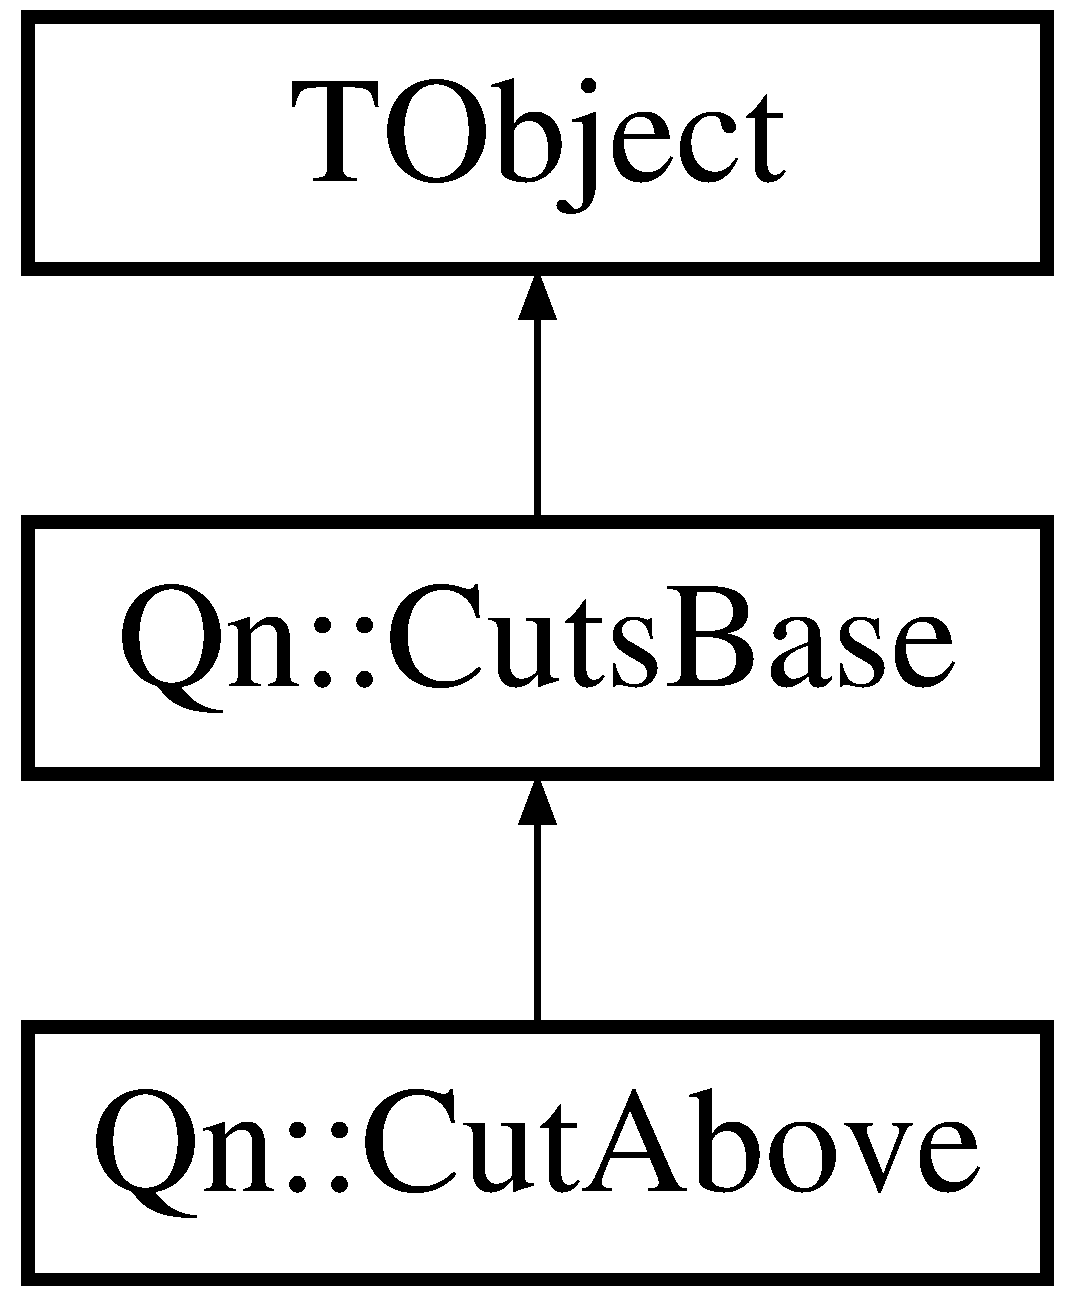
\includegraphics[height=3.000000cm]{classQn_1_1CutAbove}
\end{center}
\end{figure}
\subsection*{Public Member Functions}
\begin{DoxyCompactItemize}
\item 
\mbox{\Hypertarget{classQn_1_1CutAbove_a44c73d2c99b1ca30f53551d9bcb755e8}\label{classQn_1_1CutAbove_a44c73d2c99b1ca30f53551d9bcb755e8}} 
\mbox{\hyperlink{classQn_1_1CutAbove_a44c73d2c99b1ca30f53551d9bcb755e8}{Cut\+Above}} ()
\begin{DoxyCompactList}\small\item\em Default constructor. \end{DoxyCompactList}\item 
\mbox{\hyperlink{classQn_1_1CutAbove_a8921d1babf244944f2c5ca072fd68489}{Cut\+Above}} (const \mbox{\hyperlink{classQn_1_1CutAbove}{Cut\+Above}} \&cut)
\item 
\mbox{\hyperlink{classQn_1_1CutAbove_aa5586d4101ac6cd2720e2b1bdb608132}{Cut\+Above}} (Int\+\_\+t var\+Id, Float\+\_\+t threshold)
\item 
\mbox{\Hypertarget{classQn_1_1CutAbove_a2fab5ec0fa45bdd7d1ae52667a370857}\label{classQn_1_1CutAbove_a2fab5ec0fa45bdd7d1ae52667a370857}} 
virtual \mbox{\hyperlink{classQn_1_1CutAbove_a2fab5ec0fa45bdd7d1ae52667a370857}{$\sim$\+Cut\+Above}} ()
\begin{DoxyCompactList}\small\item\em Default destructor. Does nothing. \end{DoxyCompactList}\item 
virtual Bool\+\_\+t \mbox{\hyperlink{classQn_1_1CutAbove_a2d7ecca87d2d0c50724d795715f5cedd}{Is\+Selected}} (const double $\ast$variable\+Container)
\end{DoxyCompactItemize}
\subsection*{Additional Inherited Members}


\subsection{Constructor \& Destructor Documentation}
\mbox{\Hypertarget{classQn_1_1CutAbove_a8921d1babf244944f2c5ca072fd68489}\label{classQn_1_1CutAbove_a8921d1babf244944f2c5ca072fd68489}} 
\index{Qn\+::\+Cut\+Above@{Qn\+::\+Cut\+Above}!Cut\+Above@{Cut\+Above}}
\index{Cut\+Above@{Cut\+Above}!Qn\+::\+Cut\+Above@{Qn\+::\+Cut\+Above}}
\subsubsection{\texorpdfstring{Cut\+Above()}{CutAbove()}\hspace{0.1cm}{\footnotesize\ttfamily [1/2]}}
{\footnotesize\ttfamily Qn\+::\+Cut\+Above\+::\+Cut\+Above (\begin{DoxyParamCaption}\item[{const \mbox{\hyperlink{classQn_1_1CutAbove}{Cut\+Above}} \&}]{cut }\end{DoxyParamCaption})}

Copy constructor 
\begin{DoxyParams}{Parameters}
{\em cut} & the cut object to be cloned \\
\hline
\end{DoxyParams}
\mbox{\Hypertarget{classQn_1_1CutAbove_aa5586d4101ac6cd2720e2b1bdb608132}\label{classQn_1_1CutAbove_aa5586d4101ac6cd2720e2b1bdb608132}} 
\index{Qn\+::\+Cut\+Above@{Qn\+::\+Cut\+Above}!Cut\+Above@{Cut\+Above}}
\index{Cut\+Above@{Cut\+Above}!Qn\+::\+Cut\+Above@{Qn\+::\+Cut\+Above}}
\subsubsection{\texorpdfstring{Cut\+Above()}{CutAbove()}\hspace{0.1cm}{\footnotesize\ttfamily [2/2]}}
{\footnotesize\ttfamily Qn\+::\+Cut\+Above\+::\+Cut\+Above (\begin{DoxyParamCaption}\item[{Int\+\_\+t}]{var\+Id,  }\item[{Float\+\_\+t}]{threshold }\end{DoxyParamCaption})}

Normal constructor 
\begin{DoxyParams}{Parameters}
{\em var\+Id} & external Id for the affected variable \\
\hline
{\em threshold} & the value the variable content should be above \\
\hline
\end{DoxyParams}


\subsection{Member Function Documentation}
\mbox{\Hypertarget{classQn_1_1CutAbove_a2d7ecca87d2d0c50724d795715f5cedd}\label{classQn_1_1CutAbove_a2d7ecca87d2d0c50724d795715f5cedd}} 
\index{Qn\+::\+Cut\+Above@{Qn\+::\+Cut\+Above}!Is\+Selected@{Is\+Selected}}
\index{Is\+Selected@{Is\+Selected}!Qn\+::\+Cut\+Above@{Qn\+::\+Cut\+Above}}
\subsubsection{\texorpdfstring{Is\+Selected()}{IsSelected()}}
{\footnotesize\ttfamily Bool\+\_\+t Qn\+::\+Cut\+Above\+::\+Is\+Selected (\begin{DoxyParamCaption}\item[{const double $\ast$}]{variable\+Container }\end{DoxyParamCaption})\hspace{0.3cm}{\ttfamily [inline]}, {\ttfamily [virtual]}}

Check if the actual variable value passes the cut


\begin{DoxyParams}{Parameters}
{\em variable\+Container} & the current variables content addressed by var Id \\
\hline
\end{DoxyParams}
\begin{DoxyReturn}{Returns}
k\+T\+R\+UE if the actual value is above the threshold else k\+F\+A\+L\+SE 
\end{DoxyReturn}


Implements \mbox{\hyperlink{classQn_1_1CutsBase_aab081fa4220144505ca838539d83aa8d}{Qn\+::\+Cuts\+Base}}.



The documentation for this class was generated from the following files\+:\begin{DoxyCompactItemize}
\item 
D\+T\+\_\+\+Flow/\+Qn\+Corrections/include/Cut\+Above.\+h\item 
D\+T\+\_\+\+Flow/\+Qn\+Corrections/Cut\+Above.\+cpp\end{DoxyCompactItemize}

\hypertarget{classQn_1_1CutBelow}{}\section{Qn\+:\+:Cut\+Below Class Reference}
\label{classQn_1_1CutBelow}\index{Qn\+::\+Cut\+Below@{Qn\+::\+Cut\+Below}}
Inheritance diagram for Qn\+:\+:Cut\+Below\+:\begin{figure}[H]
\begin{center}
\leavevmode
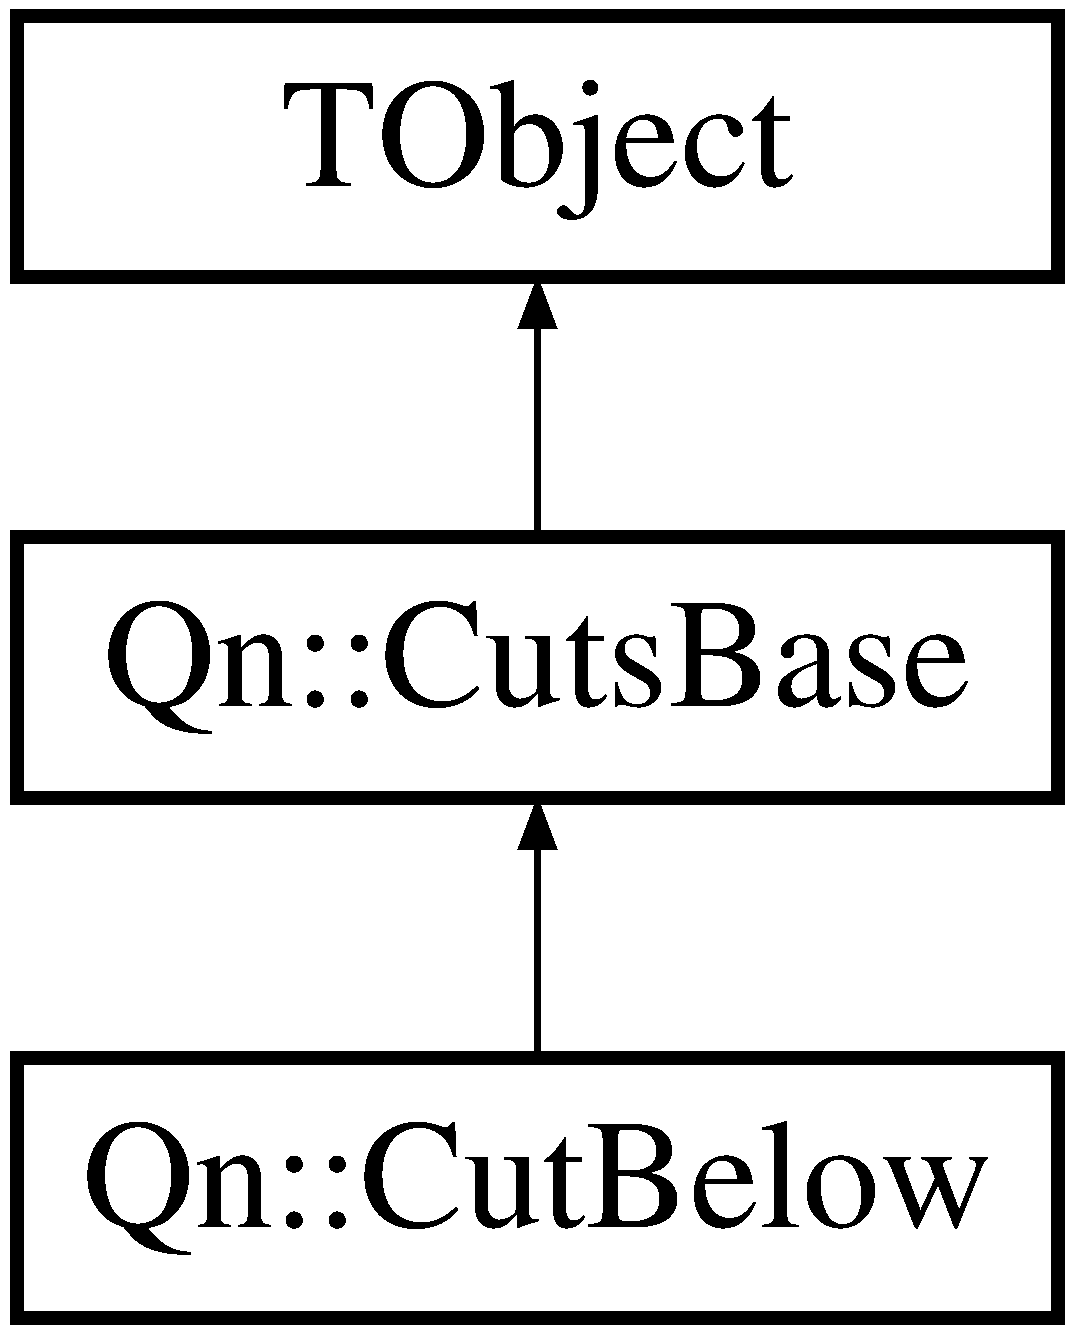
\includegraphics[height=3.000000cm]{classQn_1_1CutBelow}
\end{center}
\end{figure}
\subsection*{Public Member Functions}
\begin{DoxyCompactItemize}
\item 
\mbox{\Hypertarget{classQn_1_1CutBelow_aca2f904a16d3201a5a6ece6e644b2b82}\label{classQn_1_1CutBelow_aca2f904a16d3201a5a6ece6e644b2b82}} 
\mbox{\hyperlink{classQn_1_1CutBelow_aca2f904a16d3201a5a6ece6e644b2b82}{Cut\+Below}} ()
\begin{DoxyCompactList}\small\item\em Default constructor. \end{DoxyCompactList}\item 
\mbox{\hyperlink{classQn_1_1CutBelow_a68cce8c01e9c787e9f7fb1fcd90e9eca}{Cut\+Below}} (const \mbox{\hyperlink{classQn_1_1CutBelow}{Cut\+Below}} \&cut)
\item 
\mbox{\hyperlink{classQn_1_1CutBelow_a62dec52f3fc28e603ee8e355c4885c6b}{Cut\+Below}} (Int\+\_\+t var\+Id, Float\+\_\+t threshold)
\item 
\mbox{\Hypertarget{classQn_1_1CutBelow_a7ad873672fd0b6dcec2e865a69cf2bae}\label{classQn_1_1CutBelow_a7ad873672fd0b6dcec2e865a69cf2bae}} 
virtual \mbox{\hyperlink{classQn_1_1CutBelow_a7ad873672fd0b6dcec2e865a69cf2bae}{$\sim$\+Cut\+Below}} ()
\begin{DoxyCompactList}\small\item\em Default destructor. Does nothing. \end{DoxyCompactList}\item 
virtual Bool\+\_\+t \mbox{\hyperlink{classQn_1_1CutBelow_ae7ea2216ffcf3e65c0dd89b04ff9bf21}{Is\+Selected}} (const double $\ast$variable\+Container)
\end{DoxyCompactItemize}
\subsection*{Additional Inherited Members}


\subsection{Constructor \& Destructor Documentation}
\mbox{\Hypertarget{classQn_1_1CutBelow_a68cce8c01e9c787e9f7fb1fcd90e9eca}\label{classQn_1_1CutBelow_a68cce8c01e9c787e9f7fb1fcd90e9eca}} 
\index{Qn\+::\+Cut\+Below@{Qn\+::\+Cut\+Below}!Cut\+Below@{Cut\+Below}}
\index{Cut\+Below@{Cut\+Below}!Qn\+::\+Cut\+Below@{Qn\+::\+Cut\+Below}}
\subsubsection{\texorpdfstring{Cut\+Below()}{CutBelow()}\hspace{0.1cm}{\footnotesize\ttfamily [1/2]}}
{\footnotesize\ttfamily Qn\+::\+Cut\+Below\+::\+Cut\+Below (\begin{DoxyParamCaption}\item[{const \mbox{\hyperlink{classQn_1_1CutBelow}{Cut\+Below}} \&}]{cut }\end{DoxyParamCaption})}

Copy constructor 
\begin{DoxyParams}{Parameters}
{\em cut} & the cut object to be cloned \\
\hline
\end{DoxyParams}
\mbox{\Hypertarget{classQn_1_1CutBelow_a62dec52f3fc28e603ee8e355c4885c6b}\label{classQn_1_1CutBelow_a62dec52f3fc28e603ee8e355c4885c6b}} 
\index{Qn\+::\+Cut\+Below@{Qn\+::\+Cut\+Below}!Cut\+Below@{Cut\+Below}}
\index{Cut\+Below@{Cut\+Below}!Qn\+::\+Cut\+Below@{Qn\+::\+Cut\+Below}}
\subsubsection{\texorpdfstring{Cut\+Below()}{CutBelow()}\hspace{0.1cm}{\footnotesize\ttfamily [2/2]}}
{\footnotesize\ttfamily Qn\+::\+Cut\+Below\+::\+Cut\+Below (\begin{DoxyParamCaption}\item[{Int\+\_\+t}]{var\+Id,  }\item[{Float\+\_\+t}]{threshold }\end{DoxyParamCaption})}

Normal constructor 
\begin{DoxyParams}{Parameters}
{\em var\+Id} & external Id for the affected variable \\
\hline
{\em threshold} & the value the variable content should be below \\
\hline
\end{DoxyParams}


\subsection{Member Function Documentation}
\mbox{\Hypertarget{classQn_1_1CutBelow_ae7ea2216ffcf3e65c0dd89b04ff9bf21}\label{classQn_1_1CutBelow_ae7ea2216ffcf3e65c0dd89b04ff9bf21}} 
\index{Qn\+::\+Cut\+Below@{Qn\+::\+Cut\+Below}!Is\+Selected@{Is\+Selected}}
\index{Is\+Selected@{Is\+Selected}!Qn\+::\+Cut\+Below@{Qn\+::\+Cut\+Below}}
\subsubsection{\texorpdfstring{Is\+Selected()}{IsSelected()}}
{\footnotesize\ttfamily Bool\+\_\+t Qn\+::\+Cut\+Below\+::\+Is\+Selected (\begin{DoxyParamCaption}\item[{const double $\ast$}]{variable\+Container }\end{DoxyParamCaption})\hspace{0.3cm}{\ttfamily [inline]}, {\ttfamily [virtual]}}

Check if the actual variable value passes the cut


\begin{DoxyParams}{Parameters}
{\em variable\+Container} & the current variables content addressed by var Id \\
\hline
\end{DoxyParams}
\begin{DoxyReturn}{Returns}
k\+T\+R\+UE if the actual value is below the threshold else k\+F\+A\+L\+SE 
\end{DoxyReturn}


Implements \mbox{\hyperlink{classQn_1_1CutsBase_aab081fa4220144505ca838539d83aa8d}{Qn\+::\+Cuts\+Base}}.



The documentation for this class was generated from the following files\+:\begin{DoxyCompactItemize}
\item 
D\+T\+\_\+\+Flow/\+Qn\+Corrections/include/Cut\+Below.\+h\item 
D\+T\+\_\+\+Flow/\+Qn\+Corrections/Cut\+Below.\+cpp\end{DoxyCompactItemize}

\hypertarget{classQn_1_1CutOutside}{}\section{Qn\+:\+:Cut\+Outside Class Reference}
\label{classQn_1_1CutOutside}\index{Qn\+::\+Cut\+Outside@{Qn\+::\+Cut\+Outside}}
Inheritance diagram for Qn\+:\+:Cut\+Outside\+:\begin{figure}[H]
\begin{center}
\leavevmode
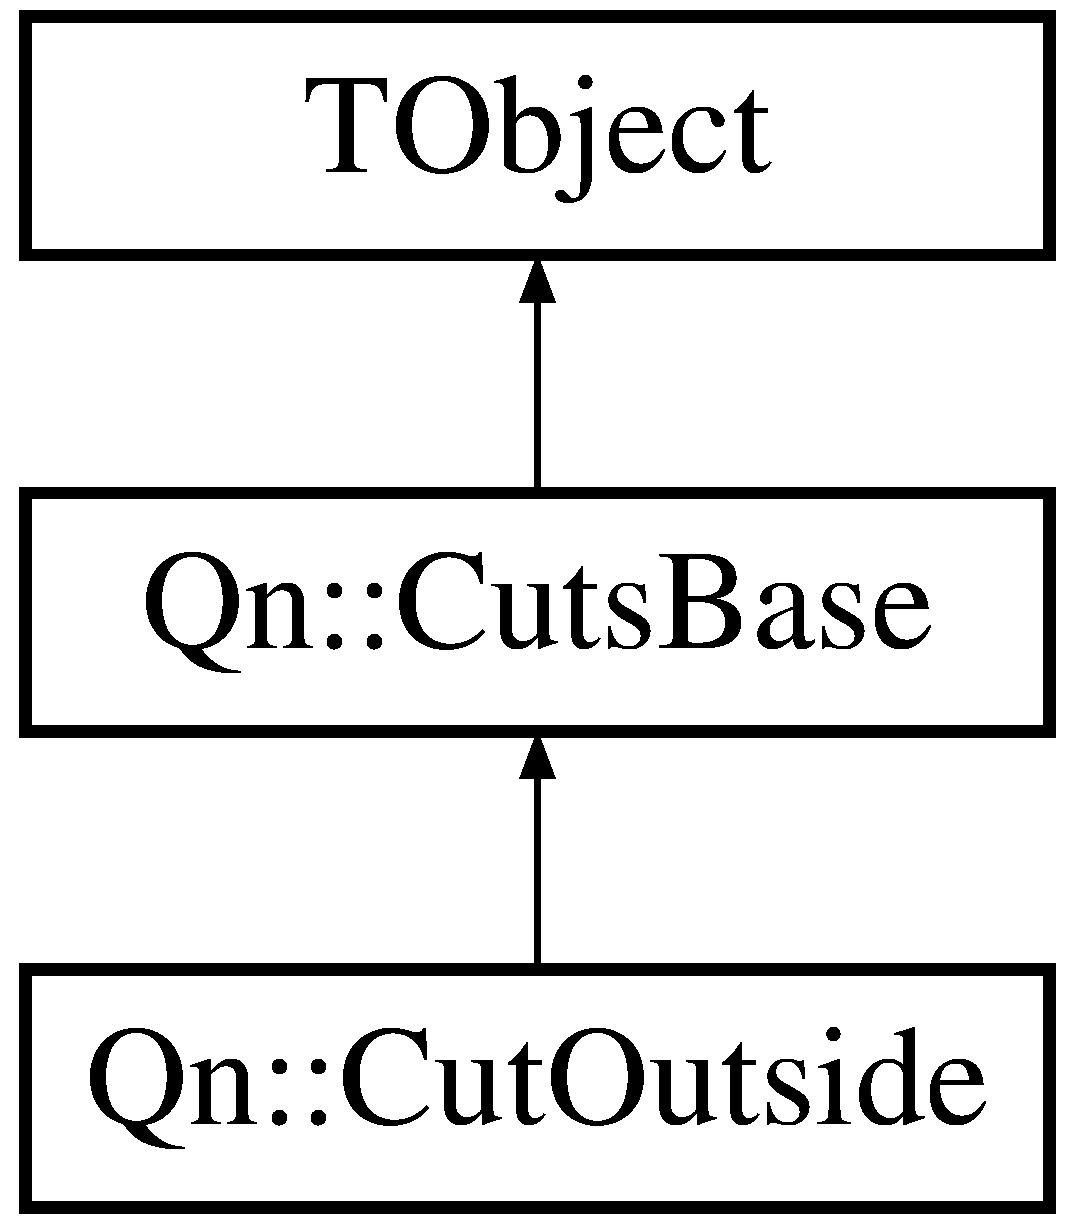
\includegraphics[height=3.000000cm]{classQn_1_1CutOutside}
\end{center}
\end{figure}
\subsection*{Public Member Functions}
\begin{DoxyCompactItemize}
\item 
\mbox{\Hypertarget{classQn_1_1CutOutside_a6667534ec2b340af943b150a642325c4}\label{classQn_1_1CutOutside_a6667534ec2b340af943b150a642325c4}} 
\mbox{\hyperlink{classQn_1_1CutOutside_a6667534ec2b340af943b150a642325c4}{Cut\+Outside}} ()
\begin{DoxyCompactList}\small\item\em Default constructor. \end{DoxyCompactList}\item 
\mbox{\hyperlink{classQn_1_1CutOutside_a58878430ec8e3cdf04bbf01551915c34}{Cut\+Outside}} (const \mbox{\hyperlink{classQn_1_1CutOutside}{Cut\+Outside}} \&cut)
\item 
\mbox{\hyperlink{classQn_1_1CutOutside_a1e47a825aaff83255e48dd4ee159ab54}{Cut\+Outside}} (Int\+\_\+t var\+Id, Float\+\_\+t min, Float\+\_\+t max)
\item 
\mbox{\Hypertarget{classQn_1_1CutOutside_a0feafa5d0b1a6ecd09629a53aef56c52}\label{classQn_1_1CutOutside_a0feafa5d0b1a6ecd09629a53aef56c52}} 
virtual \mbox{\hyperlink{classQn_1_1CutOutside_a0feafa5d0b1a6ecd09629a53aef56c52}{$\sim$\+Cut\+Outside}} ()
\begin{DoxyCompactList}\small\item\em Default destructor. Does nothing. \end{DoxyCompactList}\item 
virtual Bool\+\_\+t \mbox{\hyperlink{classQn_1_1CutOutside_ad368fe06c6b6228edbef319e73f63e24}{Is\+Selected}} (const double $\ast$variable\+Container)
\end{DoxyCompactItemize}
\subsection*{Additional Inherited Members}


\subsection{Constructor \& Destructor Documentation}
\mbox{\Hypertarget{classQn_1_1CutOutside_a58878430ec8e3cdf04bbf01551915c34}\label{classQn_1_1CutOutside_a58878430ec8e3cdf04bbf01551915c34}} 
\index{Qn\+::\+Cut\+Outside@{Qn\+::\+Cut\+Outside}!Cut\+Outside@{Cut\+Outside}}
\index{Cut\+Outside@{Cut\+Outside}!Qn\+::\+Cut\+Outside@{Qn\+::\+Cut\+Outside}}
\subsubsection{\texorpdfstring{Cut\+Outside()}{CutOutside()}\hspace{0.1cm}{\footnotesize\ttfamily [1/2]}}
{\footnotesize\ttfamily Qn\+::\+Cut\+Outside\+::\+Cut\+Outside (\begin{DoxyParamCaption}\item[{const \mbox{\hyperlink{classQn_1_1CutOutside}{Cut\+Outside}} \&}]{cut }\end{DoxyParamCaption})}

Copy constructor 
\begin{DoxyParams}{Parameters}
{\em cut} & the cut object to be cloned \\
\hline
\end{DoxyParams}
\mbox{\Hypertarget{classQn_1_1CutOutside_a1e47a825aaff83255e48dd4ee159ab54}\label{classQn_1_1CutOutside_a1e47a825aaff83255e48dd4ee159ab54}} 
\index{Qn\+::\+Cut\+Outside@{Qn\+::\+Cut\+Outside}!Cut\+Outside@{Cut\+Outside}}
\index{Cut\+Outside@{Cut\+Outside}!Qn\+::\+Cut\+Outside@{Qn\+::\+Cut\+Outside}}
\subsubsection{\texorpdfstring{Cut\+Outside()}{CutOutside()}\hspace{0.1cm}{\footnotesize\ttfamily [2/2]}}
{\footnotesize\ttfamily Qn\+::\+Cut\+Outside\+::\+Cut\+Outside (\begin{DoxyParamCaption}\item[{Int\+\_\+t}]{var\+Id,  }\item[{Float\+\_\+t}]{min,  }\item[{Float\+\_\+t}]{max }\end{DoxyParamCaption})}

Normal constructor 
\begin{DoxyParams}{Parameters}
{\em var\+Id} & external Id for the affected variable \\
\hline
{\em min} & the value the variable content should be below \\
\hline
{\em max} & the value the variable content should be above \\
\hline
\end{DoxyParams}


\subsection{Member Function Documentation}
\mbox{\Hypertarget{classQn_1_1CutOutside_ad368fe06c6b6228edbef319e73f63e24}\label{classQn_1_1CutOutside_ad368fe06c6b6228edbef319e73f63e24}} 
\index{Qn\+::\+Cut\+Outside@{Qn\+::\+Cut\+Outside}!Is\+Selected@{Is\+Selected}}
\index{Is\+Selected@{Is\+Selected}!Qn\+::\+Cut\+Outside@{Qn\+::\+Cut\+Outside}}
\subsubsection{\texorpdfstring{Is\+Selected()}{IsSelected()}}
{\footnotesize\ttfamily Bool\+\_\+t Qn\+::\+Cut\+Outside\+::\+Is\+Selected (\begin{DoxyParamCaption}\item[{const double $\ast$}]{variable\+Container }\end{DoxyParamCaption})\hspace{0.3cm}{\ttfamily [inline]}, {\ttfamily [virtual]}}

Check if the actual variable value passes the cut


\begin{DoxyParams}{Parameters}
{\em variable\+Container} & the current variables content addressed by var Id \\
\hline
\end{DoxyParams}
\begin{DoxyReturn}{Returns}
k\+T\+R\+UE if the actual value is below the threshold else k\+F\+A\+L\+SE 
\end{DoxyReturn}


Implements \mbox{\hyperlink{classQn_1_1CutsBase_aab081fa4220144505ca838539d83aa8d}{Qn\+::\+Cuts\+Base}}.



The documentation for this class was generated from the following files\+:\begin{DoxyCompactItemize}
\item 
D\+T\+\_\+\+Flow/\+Qn\+Corrections/include/Cut\+Outside.\+h\item 
D\+T\+\_\+\+Flow/\+Qn\+Corrections/Cut\+Outside.\+cpp\end{DoxyCompactItemize}

\hypertarget{classQn_1_1Cuts}{}\section{Qn\+:\+:Cuts Class Reference}
\label{classQn_1_1Cuts}\index{Qn\+::\+Cuts@{Qn\+::\+Cuts}}


{\ttfamily \#include $<$Variable\+Cut\+Base.\+h$>$}

\subsection*{Public Member Functions}
\begin{DoxyCompactItemize}
\item 
void \mbox{\hyperlink{classQn_1_1Cuts_aae5bfa081e4d3eec94422b3a8ae4213b}{Add\+Cut}} (std\+::unique\+\_\+ptr$<$ \mbox{\hyperlink{structQn_1_1VariableCutBase}{Variable\+Cut\+Base}} $>$ cut)
\begin{DoxyCompactList}\small\item\em Adds a cut to the manager. \end{DoxyCompactList}\item 
bool \mbox{\hyperlink{classQn_1_1Cuts_a9b010978523b569af5c1a40a6a03d898}{Check\+Cuts}} (int i)
\item 
\mbox{\Hypertarget{classQn_1_1Cuts_a63d2b62a2a41013d6611f71a4294b914}\label{classQn_1_1Cuts_a63d2b62a2a41013d6611f71a4294b914}} 
void \mbox{\hyperlink{classQn_1_1Cuts_a63d2b62a2a41013d6611f71a4294b914}{Fill\+Report}} ()
\begin{DoxyCompactList}\small\item\em Fills the cut report. \end{DoxyCompactList}\item 
void \mbox{\hyperlink{classQn_1_1Cuts_a4d53915785801bca58a9290149dca028}{Create\+Cut\+Report}} (std\+::string detname, std\+::size\+\_\+t nchannels=1)
\begin{DoxyCompactList}\small\item\em Initializes the cut report histogram. \end{DoxyCompactList}\item 
void \mbox{\hyperlink{classQn_1_1Cuts_ade6fa16364755bd88ed127ea8ef4cdb4}{Add\+To\+List}} (T\+List $\ast$list)
\begin{DoxyCompactList}\small\item\em Adds the cut report to the list. Lifetime of the list and the histogram has to be managed by the user. \end{DoxyCompactList}\end{DoxyCompactItemize}


\subsection{Detailed Description}
Manages cuts class and allows checking if the current variables passes the cut 

\subsection{Member Function Documentation}
\mbox{\Hypertarget{classQn_1_1Cuts_aae5bfa081e4d3eec94422b3a8ae4213b}\label{classQn_1_1Cuts_aae5bfa081e4d3eec94422b3a8ae4213b}} 
\index{Qn\+::\+Cuts@{Qn\+::\+Cuts}!Add\+Cut@{Add\+Cut}}
\index{Add\+Cut@{Add\+Cut}!Qn\+::\+Cuts@{Qn\+::\+Cuts}}
\subsubsection{\texorpdfstring{Add\+Cut()}{AddCut()}}
{\footnotesize\ttfamily void Qn\+::\+Cuts\+::\+Add\+Cut (\begin{DoxyParamCaption}\item[{std\+::unique\+\_\+ptr$<$ \mbox{\hyperlink{structQn_1_1VariableCutBase}{Variable\+Cut\+Base}} $>$}]{cut }\end{DoxyParamCaption})\hspace{0.3cm}{\ttfamily [inline]}}



Adds a cut to the manager. 


\begin{DoxyParams}{Parameters}
{\em cut} & pointer to the cut. \\
\hline
\end{DoxyParams}
\mbox{\Hypertarget{classQn_1_1Cuts_ade6fa16364755bd88ed127ea8ef4cdb4}\label{classQn_1_1Cuts_ade6fa16364755bd88ed127ea8ef4cdb4}} 
\index{Qn\+::\+Cuts@{Qn\+::\+Cuts}!Add\+To\+List@{Add\+To\+List}}
\index{Add\+To\+List@{Add\+To\+List}!Qn\+::\+Cuts@{Qn\+::\+Cuts}}
\subsubsection{\texorpdfstring{Add\+To\+List()}{AddToList()}}
{\footnotesize\ttfamily void Qn\+::\+Cuts\+::\+Add\+To\+List (\begin{DoxyParamCaption}\item[{T\+List $\ast$}]{list }\end{DoxyParamCaption})\hspace{0.3cm}{\ttfamily [inline]}}



Adds the cut report to the list. Lifetime of the list and the histogram has to be managed by the user. 


\begin{DoxyParams}{Parameters}
{\em list} & list containing output histograms. \\
\hline
\end{DoxyParams}
\mbox{\Hypertarget{classQn_1_1Cuts_a9b010978523b569af5c1a40a6a03d898}\label{classQn_1_1Cuts_a9b010978523b569af5c1a40a6a03d898}} 
\index{Qn\+::\+Cuts@{Qn\+::\+Cuts}!Check\+Cuts@{Check\+Cuts}}
\index{Check\+Cuts@{Check\+Cuts}!Qn\+::\+Cuts@{Qn\+::\+Cuts}}
\subsubsection{\texorpdfstring{Check\+Cuts()}{CheckCuts()}}
{\footnotesize\ttfamily bool Qn\+::\+Cuts\+::\+Check\+Cuts (\begin{DoxyParamCaption}\item[{int}]{i }\end{DoxyParamCaption})\hspace{0.3cm}{\ttfamily [inline]}}

Checks if the current variables pass the cuts Creates entries in the cut report 
\begin{DoxyParams}{Parameters}
{\em i} & offset of the variable in case it has a length longer than 1 \\
\hline
\end{DoxyParams}
\begin{DoxyReturn}{Returns}
Returns true if the cut was passed. 
\end{DoxyReturn}
\mbox{\Hypertarget{classQn_1_1Cuts_a4d53915785801bca58a9290149dca028}\label{classQn_1_1Cuts_a4d53915785801bca58a9290149dca028}} 
\index{Qn\+::\+Cuts@{Qn\+::\+Cuts}!Create\+Cut\+Report@{Create\+Cut\+Report}}
\index{Create\+Cut\+Report@{Create\+Cut\+Report}!Qn\+::\+Cuts@{Qn\+::\+Cuts}}
\subsubsection{\texorpdfstring{Create\+Cut\+Report()}{CreateCutReport()}}
{\footnotesize\ttfamily void Qn\+::\+Cuts\+::\+Create\+Cut\+Report (\begin{DoxyParamCaption}\item[{std\+::string}]{detname,  }\item[{std\+::size\+\_\+t}]{nchannels = {\ttfamily 1} }\end{DoxyParamCaption})\hspace{0.3cm}{\ttfamily [inline]}}



Initializes the cut report histogram. 


\begin{DoxyParams}{Parameters}
{\em detname} & name of the histogram. \\
\hline
{\em nchannels} & number of channels. \\
\hline
\end{DoxyParams}


The documentation for this class was generated from the following file\+:\begin{DoxyCompactItemize}
\item 
D\+T\+\_\+\+Flow/\+Correction/include/Variable\+Cut\+Base.\+h\end{DoxyCompactItemize}

\hypertarget{classQn_1_1CutsBase}{}\section{Qn\+:\+:Cuts\+Base Class Reference}
\label{classQn_1_1CutsBase}\index{Qn\+::\+Cuts\+Base@{Qn\+::\+Cuts\+Base}}
Inheritance diagram for Qn\+:\+:Cuts\+Base\+:\begin{figure}[H]
\begin{center}
\leavevmode
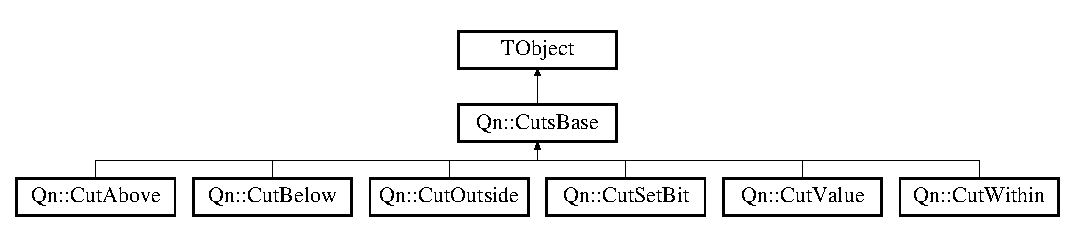
\includegraphics[height=2.666667cm]{classQn_1_1CutsBase}
\end{center}
\end{figure}
\subsection*{Public Member Functions}
\begin{DoxyCompactItemize}
\item 
\mbox{\Hypertarget{classQn_1_1CutsBase_ae3c7d2ed894bf844ccf9431797e2e3ad}\label{classQn_1_1CutsBase_ae3c7d2ed894bf844ccf9431797e2e3ad}} 
\mbox{\hyperlink{classQn_1_1CutsBase_ae3c7d2ed894bf844ccf9431797e2e3ad}{Cuts\+Base}} ()
\begin{DoxyCompactList}\small\item\em Default constructor. \end{DoxyCompactList}\item 
\mbox{\hyperlink{classQn_1_1CutsBase_a5b86fd2a224c93e313c545e926d30539}{Cuts\+Base}} (const \mbox{\hyperlink{classQn_1_1CutsBase}{Cuts\+Base}} \&cut)
\item 
\mbox{\hyperlink{classQn_1_1CutsBase_a0b506ca7d770a8d5991b7f22848e7b81}{Cuts\+Base}} (Int\+\_\+t var\+Id)
\item 
\mbox{\Hypertarget{classQn_1_1CutsBase_ad000d14b6b95500bee244aedb0086813}\label{classQn_1_1CutsBase_ad000d14b6b95500bee244aedb0086813}} 
virtual \mbox{\hyperlink{classQn_1_1CutsBase_ad000d14b6b95500bee244aedb0086813}{$\sim$\+Cuts\+Base}} ()
\begin{DoxyCompactList}\small\item\em Default destructor. Does nothing. \end{DoxyCompactList}\item 
\mbox{\Hypertarget{classQn_1_1CutsBase_a9fcdc1df927edefd1c6fe772d4a70ea2}\label{classQn_1_1CutsBase_a9fcdc1df927edefd1c6fe772d4a70ea2}} 
Int\+\_\+t \mbox{\hyperlink{classQn_1_1CutsBase_a9fcdc1df927edefd1c6fe772d4a70ea2}{Get\+Variable\+Id}} () const
\begin{DoxyCompactList}\small\item\em Gets the variable Id the cut is applied to. \end{DoxyCompactList}\item 
virtual Bool\+\_\+t \mbox{\hyperlink{classQn_1_1CutsBase_aab081fa4220144505ca838539d83aa8d}{Is\+Selected}} (const double $\ast$variable\+Container)=0
\end{DoxyCompactItemize}
\subsection*{Protected Attributes}
\begin{DoxyCompactItemize}
\item 
\mbox{\Hypertarget{classQn_1_1CutsBase_a9015a1d598b82d725128c027c6739715}\label{classQn_1_1CutsBase_a9015a1d598b82d725128c027c6739715}} 
Int\+\_\+t \mbox{\hyperlink{classQn_1_1CutsBase_a9015a1d598b82d725128c027c6739715}{f\+Var\+Id}}
\begin{DoxyCompactList}\small\item\em The external Id for the variable in the data bank. \end{DoxyCompactList}\end{DoxyCompactItemize}
\subsection*{Static Protected Attributes}
\begin{DoxyCompactItemize}
\item 
\mbox{\Hypertarget{classQn_1_1CutsBase_a2fe9ccf5025f6d78b3a45a4d8202584e}\label{classQn_1_1CutsBase_a2fe9ccf5025f6d78b3a45a4d8202584e}} 
static const Int\+\_\+t \mbox{\hyperlink{classQn_1_1CutsBase_a2fe9ccf5025f6d78b3a45a4d8202584e}{n\+Highest\+Bit\+Number\+Supported}} = 31
\begin{DoxyCompactList}\small\item\em The highest bit number the framework support. \end{DoxyCompactList}\end{DoxyCompactItemize}


\subsection{Constructor \& Destructor Documentation}
\mbox{\Hypertarget{classQn_1_1CutsBase_a5b86fd2a224c93e313c545e926d30539}\label{classQn_1_1CutsBase_a5b86fd2a224c93e313c545e926d30539}} 
\index{Qn\+::\+Cuts\+Base@{Qn\+::\+Cuts\+Base}!Cuts\+Base@{Cuts\+Base}}
\index{Cuts\+Base@{Cuts\+Base}!Qn\+::\+Cuts\+Base@{Qn\+::\+Cuts\+Base}}
\subsubsection{\texorpdfstring{Cuts\+Base()}{CutsBase()}\hspace{0.1cm}{\footnotesize\ttfamily [1/2]}}
{\footnotesize\ttfamily Qn\+::\+Cuts\+Base\+::\+Cuts\+Base (\begin{DoxyParamCaption}\item[{const \mbox{\hyperlink{classQn_1_1CutsBase}{Cuts\+Base}} \&}]{cut }\end{DoxyParamCaption})}

Copy constructor 
\begin{DoxyParams}{Parameters}
{\em cut} & the cut object to clone \\
\hline
\end{DoxyParams}
\mbox{\Hypertarget{classQn_1_1CutsBase_a0b506ca7d770a8d5991b7f22848e7b81}\label{classQn_1_1CutsBase_a0b506ca7d770a8d5991b7f22848e7b81}} 
\index{Qn\+::\+Cuts\+Base@{Qn\+::\+Cuts\+Base}!Cuts\+Base@{Cuts\+Base}}
\index{Cuts\+Base@{Cuts\+Base}!Qn\+::\+Cuts\+Base@{Qn\+::\+Cuts\+Base}}
\subsubsection{\texorpdfstring{Cuts\+Base()}{CutsBase()}\hspace{0.1cm}{\footnotesize\ttfamily [2/2]}}
{\footnotesize\ttfamily Qn\+::\+Cuts\+Base\+::\+Cuts\+Base (\begin{DoxyParamCaption}\item[{Int\+\_\+t}]{var\+Id }\end{DoxyParamCaption})}

Normal constructor. Stores the affected variable Id 
\begin{DoxyParams}{Parameters}
{\em var\+Id} & External Id for the affected variable \\
\hline
\end{DoxyParams}


\subsection{Member Function Documentation}
\mbox{\Hypertarget{classQn_1_1CutsBase_aab081fa4220144505ca838539d83aa8d}\label{classQn_1_1CutsBase_aab081fa4220144505ca838539d83aa8d}} 
\index{Qn\+::\+Cuts\+Base@{Qn\+::\+Cuts\+Base}!Is\+Selected@{Is\+Selected}}
\index{Is\+Selected@{Is\+Selected}!Qn\+::\+Cuts\+Base@{Qn\+::\+Cuts\+Base}}
\subsubsection{\texorpdfstring{Is\+Selected()}{IsSelected()}}
{\footnotesize\ttfamily virtual Bool\+\_\+t Qn\+::\+Cuts\+Base\+::\+Is\+Selected (\begin{DoxyParamCaption}\item[{const double $\ast$}]{variable\+Container }\end{DoxyParamCaption})\hspace{0.3cm}{\ttfamily [pure virtual]}}

Check if the actual variable value passes the cut

Interface declaration function. Default behavior. \mbox{\hyperlink{classBase}{Base}} class should not be instantiated.


\begin{DoxyParams}{Parameters}
{\em variable\+Container} & the current variables content addressed by var Id \\
\hline
\end{DoxyParams}
\begin{DoxyReturn}{Returns}
k\+T\+R\+UE if the actual value passes the cut else k\+F\+A\+L\+SE 
\end{DoxyReturn}


Implemented in \mbox{\hyperlink{classQn_1_1CutSetBit_a8881f7abf183ff353492a3c96862081e}{Qn\+::\+Cut\+Set\+Bit}}, \mbox{\hyperlink{classQn_1_1CutOutside_ad368fe06c6b6228edbef319e73f63e24}{Qn\+::\+Cut\+Outside}}, \mbox{\hyperlink{classQn_1_1CutValue_acdfa89e7784423f4beaea51deafd424f}{Qn\+::\+Cut\+Value}}, \mbox{\hyperlink{classQn_1_1CutWithin_a0766a4ec99389a9991ee8f2c974bdaf4}{Qn\+::\+Cut\+Within}}, \mbox{\hyperlink{classQn_1_1CutAbove_a2d7ecca87d2d0c50724d795715f5cedd}{Qn\+::\+Cut\+Above}}, and \mbox{\hyperlink{classQn_1_1CutBelow_ae7ea2216ffcf3e65c0dd89b04ff9bf21}{Qn\+::\+Cut\+Below}}.



The documentation for this class was generated from the following files\+:\begin{DoxyCompactItemize}
\item 
D\+T\+\_\+\+Flow/\+Qn\+Corrections/include/Cuts\+Base.\+h\item 
D\+T\+\_\+\+Flow/\+Qn\+Corrections/Cuts\+Base.\+cpp\end{DoxyCompactItemize}

\hypertarget{classQn_1_1CutSetBit}{}\section{Qn\+:\+:Cut\+Set\+Bit Class Reference}
\label{classQn_1_1CutSetBit}\index{Qn\+::\+Cut\+Set\+Bit@{Qn\+::\+Cut\+Set\+Bit}}
Inheritance diagram for Qn\+:\+:Cut\+Set\+Bit\+:\begin{figure}[H]
\begin{center}
\leavevmode
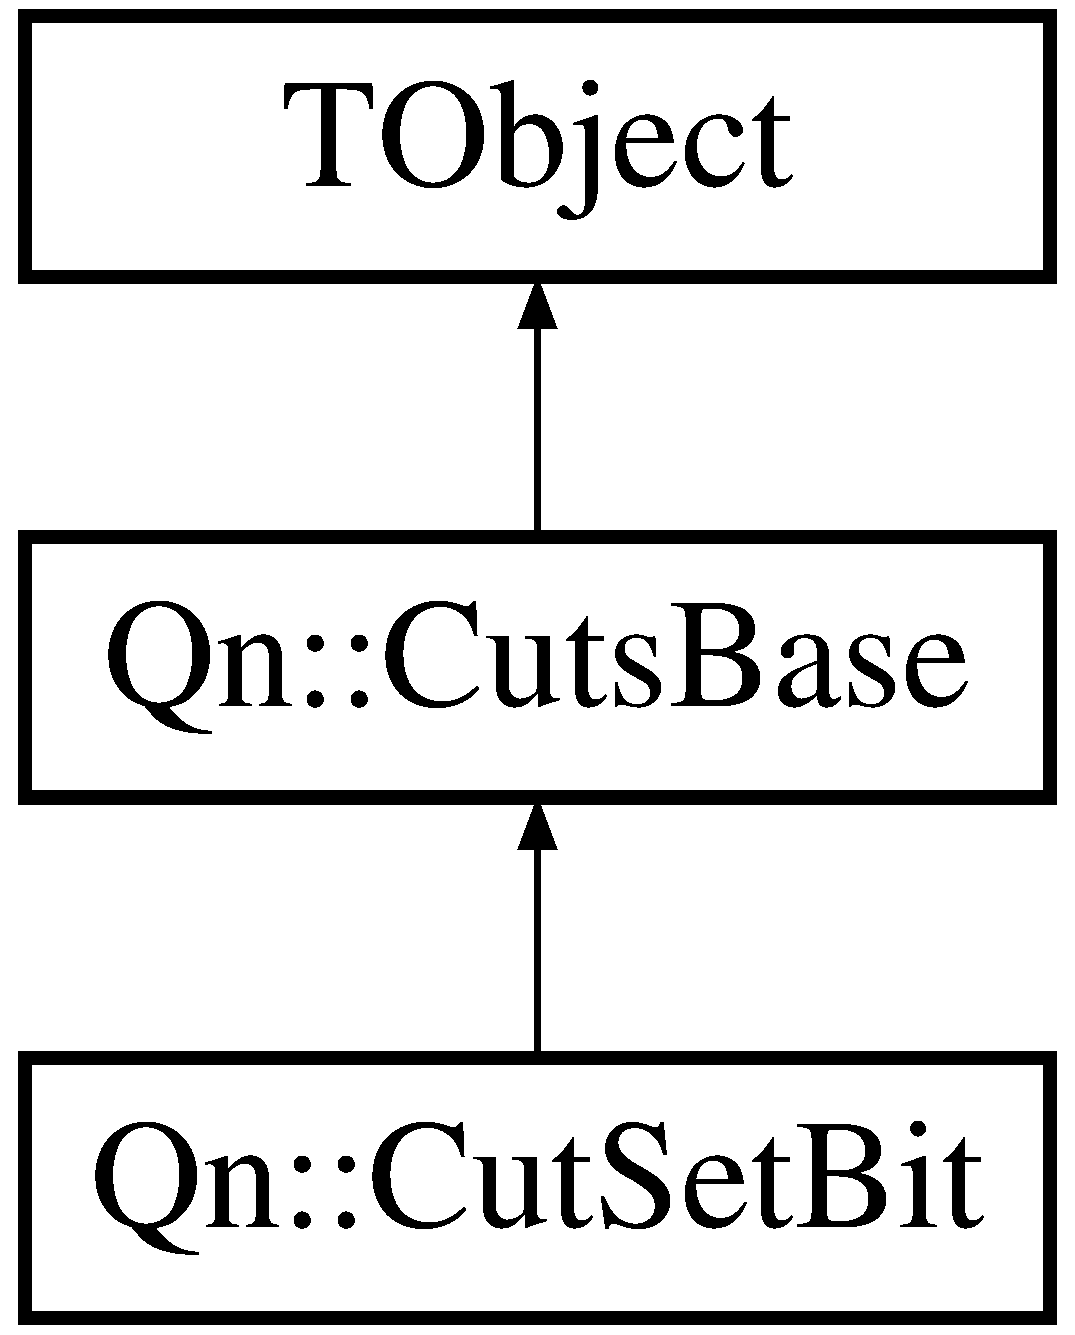
\includegraphics[height=3.000000cm]{classQn_1_1CutSetBit}
\end{center}
\end{figure}
\subsection*{Public Member Functions}
\begin{DoxyCompactItemize}
\item 
\mbox{\Hypertarget{classQn_1_1CutSetBit_a756c100ffa84f2b94d426582c0d423a7}\label{classQn_1_1CutSetBit_a756c100ffa84f2b94d426582c0d423a7}} 
\mbox{\hyperlink{classQn_1_1CutSetBit_a756c100ffa84f2b94d426582c0d423a7}{Cut\+Set\+Bit}} ()
\begin{DoxyCompactList}\small\item\em Default constructor. \end{DoxyCompactList}\item 
\mbox{\hyperlink{classQn_1_1CutSetBit_adb4e4a353d808dac2bdeeeb534600444}{Cut\+Set\+Bit}} (const \mbox{\hyperlink{classQn_1_1CutSetBit}{Cut\+Set\+Bit}} \&cut)
\item 
\mbox{\hyperlink{classQn_1_1CutSetBit_af27d1e31ca426cd6c8eba43ffcd099c1}{Cut\+Set\+Bit}} (Int\+\_\+t var\+Id, Int\+\_\+t bit\+No, Bool\+\_\+t set)
\item 
\mbox{\Hypertarget{classQn_1_1CutSetBit_a712e41a80433dda2a5afab70e09e744b}\label{classQn_1_1CutSetBit_a712e41a80433dda2a5afab70e09e744b}} 
virtual \mbox{\hyperlink{classQn_1_1CutSetBit_a712e41a80433dda2a5afab70e09e744b}{$\sim$\+Cut\+Set\+Bit}} ()
\begin{DoxyCompactList}\small\item\em Default destructor. Does nothing. \end{DoxyCompactList}\item 
virtual Bool\+\_\+t \mbox{\hyperlink{classQn_1_1CutSetBit_a8881f7abf183ff353492a3c96862081e}{Is\+Selected}} (const double $\ast$variable\+Container)
\end{DoxyCompactItemize}
\subsection*{Additional Inherited Members}


\subsection{Constructor \& Destructor Documentation}
\mbox{\Hypertarget{classQn_1_1CutSetBit_adb4e4a353d808dac2bdeeeb534600444}\label{classQn_1_1CutSetBit_adb4e4a353d808dac2bdeeeb534600444}} 
\index{Qn\+::\+Cut\+Set\+Bit@{Qn\+::\+Cut\+Set\+Bit}!Cut\+Set\+Bit@{Cut\+Set\+Bit}}
\index{Cut\+Set\+Bit@{Cut\+Set\+Bit}!Qn\+::\+Cut\+Set\+Bit@{Qn\+::\+Cut\+Set\+Bit}}
\subsubsection{\texorpdfstring{Cut\+Set\+Bit()}{CutSetBit()}\hspace{0.1cm}{\footnotesize\ttfamily [1/2]}}
{\footnotesize\ttfamily Qn\+::\+Cut\+Set\+Bit\+::\+Cut\+Set\+Bit (\begin{DoxyParamCaption}\item[{const \mbox{\hyperlink{classQn_1_1CutSetBit}{Cut\+Set\+Bit}} \&}]{cut }\end{DoxyParamCaption})}

Copy constructor 
\begin{DoxyParams}{Parameters}
{\em cut} & the cut object to be cloned \\
\hline
\end{DoxyParams}
\mbox{\Hypertarget{classQn_1_1CutSetBit_af27d1e31ca426cd6c8eba43ffcd099c1}\label{classQn_1_1CutSetBit_af27d1e31ca426cd6c8eba43ffcd099c1}} 
\index{Qn\+::\+Cut\+Set\+Bit@{Qn\+::\+Cut\+Set\+Bit}!Cut\+Set\+Bit@{Cut\+Set\+Bit}}
\index{Cut\+Set\+Bit@{Cut\+Set\+Bit}!Qn\+::\+Cut\+Set\+Bit@{Qn\+::\+Cut\+Set\+Bit}}
\subsubsection{\texorpdfstring{Cut\+Set\+Bit()}{CutSetBit()}\hspace{0.1cm}{\footnotesize\ttfamily [2/2]}}
{\footnotesize\ttfamily Qn\+::\+Cut\+Set\+Bit\+::\+Cut\+Set\+Bit (\begin{DoxyParamCaption}\item[{Int\+\_\+t}]{var\+Id,  }\item[{Int\+\_\+t}]{bit\+No,  }\item[{Bool\+\_\+t}]{set }\end{DoxyParamCaption})}

Normal constructor 
\begin{DoxyParams}{Parameters}
{\em var\+Id} & external Id for the affected variable \\
\hline
{\em bit\+No} & the bit on the variable content to test (from 0 to 31) \\
\hline
{\em set} & (k\+F\+A\+L\+SE)k\+T\+R\+UE for cut on the bit (un)set \\
\hline
\end{DoxyParams}


\subsection{Member Function Documentation}
\mbox{\Hypertarget{classQn_1_1CutSetBit_a8881f7abf183ff353492a3c96862081e}\label{classQn_1_1CutSetBit_a8881f7abf183ff353492a3c96862081e}} 
\index{Qn\+::\+Cut\+Set\+Bit@{Qn\+::\+Cut\+Set\+Bit}!Is\+Selected@{Is\+Selected}}
\index{Is\+Selected@{Is\+Selected}!Qn\+::\+Cut\+Set\+Bit@{Qn\+::\+Cut\+Set\+Bit}}
\subsubsection{\texorpdfstring{Is\+Selected()}{IsSelected()}}
{\footnotesize\ttfamily Bool\+\_\+t Qn\+::\+Cut\+Set\+Bit\+::\+Is\+Selected (\begin{DoxyParamCaption}\item[{const double $\ast$}]{variable\+Container }\end{DoxyParamCaption})\hspace{0.3cm}{\ttfamily [inline]}, {\ttfamily [virtual]}}

Check if the actual variable value passes the cut


\begin{DoxyParams}{Parameters}
{\em variable\+Container} & the current variables content addressed by var Id \\
\hline
\end{DoxyParams}
\begin{DoxyReturn}{Returns}
k\+T\+R\+UE if the actual value is below the threshold else k\+F\+A\+L\+SE 
\end{DoxyReturn}


Implements \mbox{\hyperlink{classQn_1_1CutsBase_aab081fa4220144505ca838539d83aa8d}{Qn\+::\+Cuts\+Base}}.



The documentation for this class was generated from the following files\+:\begin{DoxyCompactItemize}
\item 
D\+T\+\_\+\+Flow/\+Qn\+Corrections/include/Cut\+Set\+Bit.\+h\item 
D\+T\+\_\+\+Flow/\+Qn\+Corrections/Cut\+Set\+Bit.\+cpp\end{DoxyCompactItemize}

\hypertarget{classQn_1_1CutsSet}{}\section{Qn\+:\+:Cuts\+Set Class Reference}
\label{classQn_1_1CutsSet}\index{Qn\+::\+Cuts\+Set@{Qn\+::\+Cuts\+Set}}
Inheritance diagram for Qn\+:\+:Cuts\+Set\+:\begin{figure}[H]
\begin{center}
\leavevmode
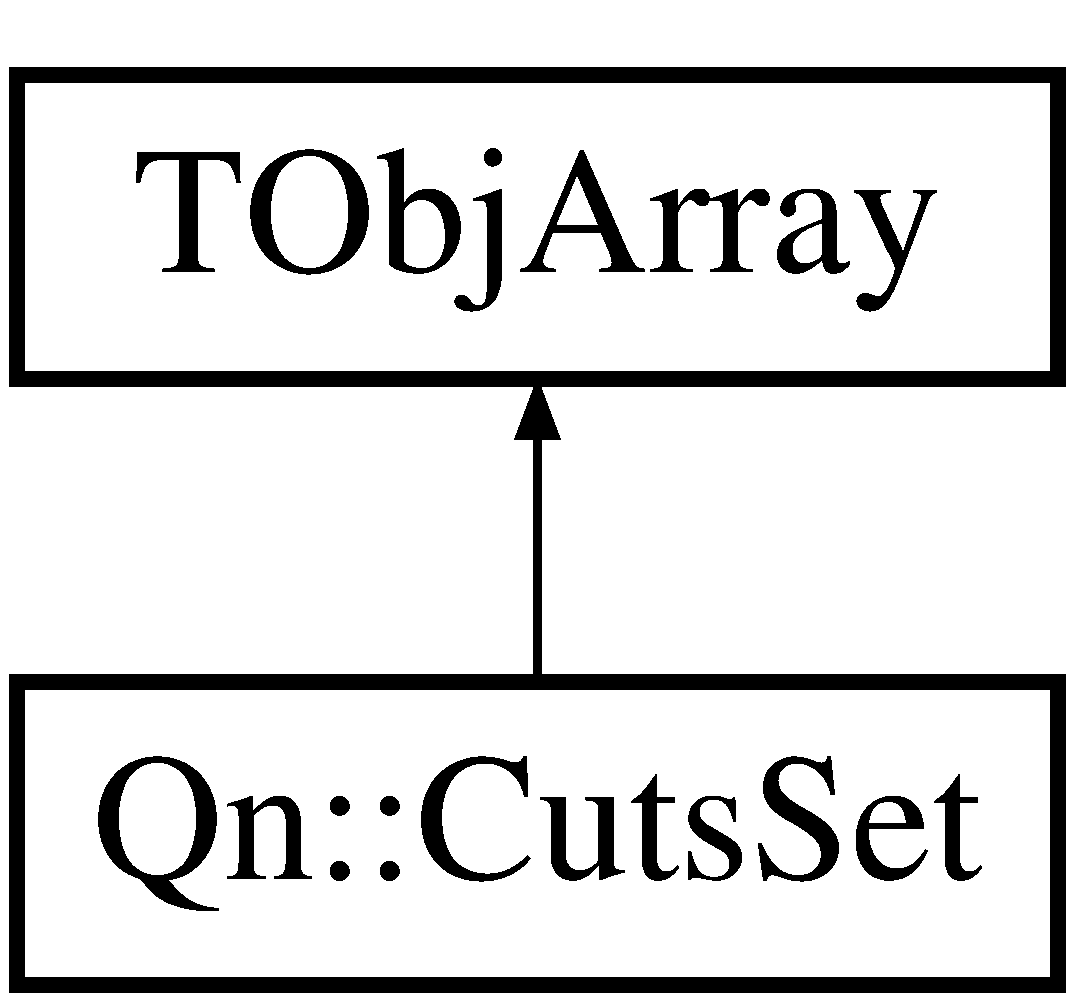
\includegraphics[height=2.000000cm]{classQn_1_1CutsSet}
\end{center}
\end{figure}
\subsection*{Public Member Functions}
\begin{DoxyCompactItemize}
\item 
\mbox{\hyperlink{classQn_1_1CutsSet_abb692440b7ffadcf3a0b5881fc1906c8}{Cuts\+Set}} (Int\+\_\+t n=T\+Collection\+::k\+Init\+Capacity)
\item 
\mbox{\hyperlink{classQn_1_1CutsSet_ac8b055e82b9f8dbb70c427525543a6a2}{Cuts\+Set}} (const \mbox{\hyperlink{classQn_1_1CutsSet}{Cuts\+Set}} \&ccs)
\item 
\mbox{\Hypertarget{classQn_1_1CutsSet_ad10fa23d0dc5e73f22d067111be6ed76}\label{classQn_1_1CutsSet_ad10fa23d0dc5e73f22d067111be6ed76}} 
virtual \mbox{\hyperlink{classQn_1_1CutsSet_ad10fa23d0dc5e73f22d067111be6ed76}{$\sim$\+Cuts\+Set}} ()
\begin{DoxyCompactList}\small\item\em Default destructor. \end{DoxyCompactList}\item 
virtual \mbox{\hyperlink{classQn_1_1CutsBase}{Cuts\+Base}} $\ast$ \mbox{\hyperlink{classQn_1_1CutsSet_a2f572076ba27d9031975fc38dc160d12}{At}} (Int\+\_\+t i) const
\item 
Bool\+\_\+t \mbox{\hyperlink{classQn_1_1CutsSet_a69dc9eba4cdb1e1270bb9340212f20b7}{Is\+Selected}} (const double $\ast$variable\+Container)
\end{DoxyCompactItemize}


\subsection{Constructor \& Destructor Documentation}
\mbox{\Hypertarget{classQn_1_1CutsSet_abb692440b7ffadcf3a0b5881fc1906c8}\label{classQn_1_1CutsSet_abb692440b7ffadcf3a0b5881fc1906c8}} 
\index{Qn\+::\+Cuts\+Set@{Qn\+::\+Cuts\+Set}!Cuts\+Set@{Cuts\+Set}}
\index{Cuts\+Set@{Cuts\+Set}!Qn\+::\+Cuts\+Set@{Qn\+::\+Cuts\+Set}}
\subsubsection{\texorpdfstring{Cuts\+Set()}{CutsSet()}\hspace{0.1cm}{\footnotesize\ttfamily [1/2]}}
{\footnotesize\ttfamily Qn\+::\+Cuts\+Set\+::\+Cuts\+Set (\begin{DoxyParamCaption}\item[{Int\+\_\+t}]{n = {\ttfamily TCollection\+:\+:kInitCapacity} }\end{DoxyParamCaption})\hspace{0.3cm}{\ttfamily [inline]}}

Normal constructor 
\begin{DoxyParams}{Parameters}
{\em n} & number of cuts in the set \\
\hline
\end{DoxyParams}
\mbox{\Hypertarget{classQn_1_1CutsSet_ac8b055e82b9f8dbb70c427525543a6a2}\label{classQn_1_1CutsSet_ac8b055e82b9f8dbb70c427525543a6a2}} 
\index{Qn\+::\+Cuts\+Set@{Qn\+::\+Cuts\+Set}!Cuts\+Set@{Cuts\+Set}}
\index{Cuts\+Set@{Cuts\+Set}!Qn\+::\+Cuts\+Set@{Qn\+::\+Cuts\+Set}}
\subsubsection{\texorpdfstring{Cuts\+Set()}{CutsSet()}\hspace{0.1cm}{\footnotesize\ttfamily [2/2]}}
{\footnotesize\ttfamily Qn\+::\+Cuts\+Set\+::\+Cuts\+Set (\begin{DoxyParamCaption}\item[{const \mbox{\hyperlink{classQn_1_1CutsSet}{Cuts\+Set}} \&}]{ccs }\end{DoxyParamCaption})\hspace{0.3cm}{\ttfamily [inline]}}

Copy constructor 
\begin{DoxyParams}{Parameters}
{\em ccs} & the object instance to be copied \\
\hline
\end{DoxyParams}


\subsection{Member Function Documentation}
\mbox{\Hypertarget{classQn_1_1CutsSet_a2f572076ba27d9031975fc38dc160d12}\label{classQn_1_1CutsSet_a2f572076ba27d9031975fc38dc160d12}} 
\index{Qn\+::\+Cuts\+Set@{Qn\+::\+Cuts\+Set}!At@{At}}
\index{At@{At}!Qn\+::\+Cuts\+Set@{Qn\+::\+Cuts\+Set}}
\subsubsection{\texorpdfstring{At()}{At()}}
{\footnotesize\ttfamily virtual \mbox{\hyperlink{classQn_1_1CutsBase}{Cuts\+Base}}$\ast$ Qn\+::\+Cuts\+Set\+::\+At (\begin{DoxyParamCaption}\item[{Int\+\_\+t}]{i }\end{DoxyParamCaption}) const\hspace{0.3cm}{\ttfamily [inline]}, {\ttfamily [virtual]}}

Access the event class variable at the passed position 
\begin{DoxyParams}{Parameters}
{\em i} & position in the array (starting at zero) \\
\hline
\end{DoxyParams}
\begin{DoxyReturn}{Returns}
the event class variable object a position i 
\end{DoxyReturn}
\mbox{\Hypertarget{classQn_1_1CutsSet_a69dc9eba4cdb1e1270bb9340212f20b7}\label{classQn_1_1CutsSet_a69dc9eba4cdb1e1270bb9340212f20b7}} 
\index{Qn\+::\+Cuts\+Set@{Qn\+::\+Cuts\+Set}!Is\+Selected@{Is\+Selected}}
\index{Is\+Selected@{Is\+Selected}!Qn\+::\+Cuts\+Set@{Qn\+::\+Cuts\+Set}}
\subsubsection{\texorpdfstring{Is\+Selected()}{IsSelected()}}
{\footnotesize\ttfamily Bool\+\_\+t Qn\+::\+Cuts\+Set\+::\+Is\+Selected (\begin{DoxyParamCaption}\item[{const double $\ast$}]{variable\+Container }\end{DoxyParamCaption})\hspace{0.3cm}{\ttfamily [inline]}}

Checks that the current content of the variable\+Container passes the whole set of cuts by going through all the array components


\begin{DoxyParams}{Parameters}
{\em variable\+Container} & the current variables content addressed by var Id \\
\hline
\end{DoxyParams}
\begin{DoxyReturn}{Returns}
k\+T\+R\+UE if the actual values pass the set of cuts else k\+F\+A\+L\+SE 
\end{DoxyReturn}


The documentation for this class was generated from the following file\+:\begin{DoxyCompactItemize}
\item 
D\+T\+\_\+\+Flow/\+Qn\+Corrections/include/Cuts\+Set.\+h\end{DoxyCompactItemize}

\hypertarget{classQn_1_1CutValue}{}\section{Qn\+:\+:Cut\+Value Class Reference}
\label{classQn_1_1CutValue}\index{Qn\+::\+Cut\+Value@{Qn\+::\+Cut\+Value}}
Inheritance diagram for Qn\+:\+:Cut\+Value\+:\begin{figure}[H]
\begin{center}
\leavevmode
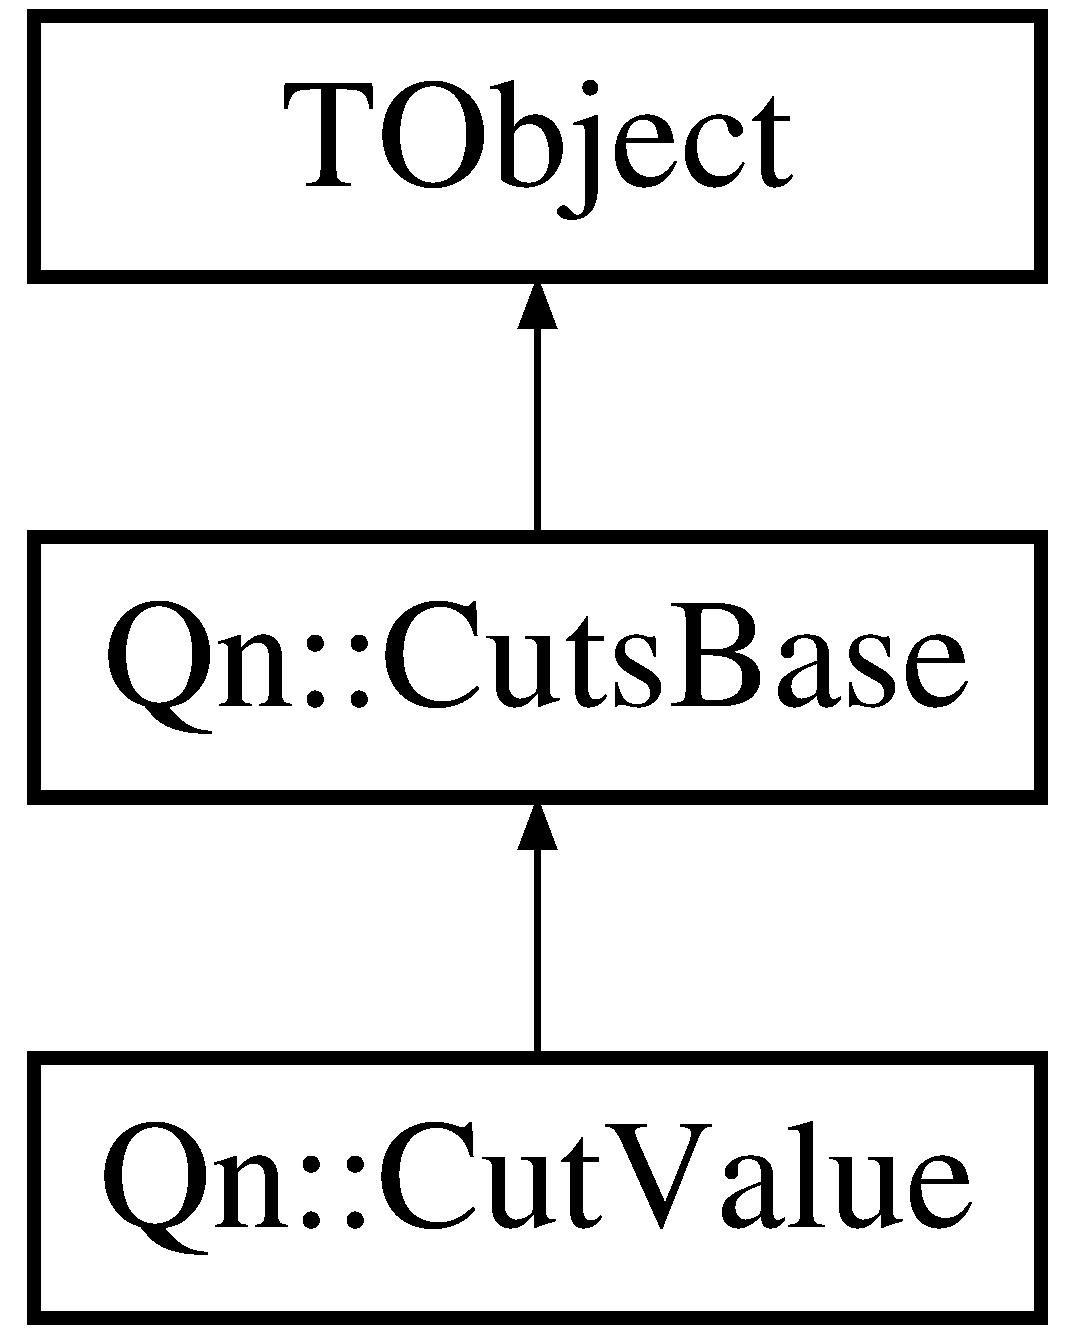
\includegraphics[height=3.000000cm]{classQn_1_1CutValue}
\end{center}
\end{figure}
\subsection*{Public Member Functions}
\begin{DoxyCompactItemize}
\item 
\mbox{\Hypertarget{classQn_1_1CutValue_ab516a2ca2aa3f9242ccc5c85644f18d9}\label{classQn_1_1CutValue_ab516a2ca2aa3f9242ccc5c85644f18d9}} 
\mbox{\hyperlink{classQn_1_1CutValue_ab516a2ca2aa3f9242ccc5c85644f18d9}{Cut\+Value}} ()
\begin{DoxyCompactList}\small\item\em Default constructor. \end{DoxyCompactList}\item 
\mbox{\hyperlink{classQn_1_1CutValue_af631798a1a977d81ff8fdb37bcb6abd4}{Cut\+Value}} (const \mbox{\hyperlink{classQn_1_1CutValue}{Cut\+Value}} \&cut)
\item 
\mbox{\hyperlink{classQn_1_1CutValue_a85b618f1f7f26f786311a964bc1509e8}{Cut\+Value}} (Int\+\_\+t var\+Id, Float\+\_\+t value)
\item 
\mbox{\Hypertarget{classQn_1_1CutValue_ac38331929f308d7e04a81239234638e5}\label{classQn_1_1CutValue_ac38331929f308d7e04a81239234638e5}} 
virtual \mbox{\hyperlink{classQn_1_1CutValue_ac38331929f308d7e04a81239234638e5}{$\sim$\+Cut\+Value}} ()
\begin{DoxyCompactList}\small\item\em Default destructor. Does nothing. \end{DoxyCompactList}\item 
virtual Bool\+\_\+t \mbox{\hyperlink{classQn_1_1CutValue_acdfa89e7784423f4beaea51deafd424f}{Is\+Selected}} (const double $\ast$variable\+Container)
\end{DoxyCompactItemize}
\subsection*{Additional Inherited Members}


\subsection{Constructor \& Destructor Documentation}
\mbox{\Hypertarget{classQn_1_1CutValue_af631798a1a977d81ff8fdb37bcb6abd4}\label{classQn_1_1CutValue_af631798a1a977d81ff8fdb37bcb6abd4}} 
\index{Qn\+::\+Cut\+Value@{Qn\+::\+Cut\+Value}!Cut\+Value@{Cut\+Value}}
\index{Cut\+Value@{Cut\+Value}!Qn\+::\+Cut\+Value@{Qn\+::\+Cut\+Value}}
\subsubsection{\texorpdfstring{Cut\+Value()}{CutValue()}\hspace{0.1cm}{\footnotesize\ttfamily [1/2]}}
{\footnotesize\ttfamily Qn\+::\+Cut\+Value\+::\+Cut\+Value (\begin{DoxyParamCaption}\item[{const \mbox{\hyperlink{classQn_1_1CutValue}{Cut\+Value}} \&}]{cut }\end{DoxyParamCaption})}

Copy constructor 
\begin{DoxyParams}{Parameters}
{\em cut} & the cut object to be cloned \\
\hline
\end{DoxyParams}
\mbox{\Hypertarget{classQn_1_1CutValue_a85b618f1f7f26f786311a964bc1509e8}\label{classQn_1_1CutValue_a85b618f1f7f26f786311a964bc1509e8}} 
\index{Qn\+::\+Cut\+Value@{Qn\+::\+Cut\+Value}!Cut\+Value@{Cut\+Value}}
\index{Cut\+Value@{Cut\+Value}!Qn\+::\+Cut\+Value@{Qn\+::\+Cut\+Value}}
\subsubsection{\texorpdfstring{Cut\+Value()}{CutValue()}\hspace{0.1cm}{\footnotesize\ttfamily [2/2]}}
{\footnotesize\ttfamily Qn\+::\+Cut\+Value\+::\+Cut\+Value (\begin{DoxyParamCaption}\item[{Int\+\_\+t}]{var\+Id,  }\item[{Float\+\_\+t}]{value }\end{DoxyParamCaption})}

Normal constructor 
\begin{DoxyParams}{Parameters}
{\em var\+Id} & external Id for the affected variable \\
\hline
{\em value} & the value the variable content should be equal to \\
\hline
\end{DoxyParams}


\subsection{Member Function Documentation}
\mbox{\Hypertarget{classQn_1_1CutValue_acdfa89e7784423f4beaea51deafd424f}\label{classQn_1_1CutValue_acdfa89e7784423f4beaea51deafd424f}} 
\index{Qn\+::\+Cut\+Value@{Qn\+::\+Cut\+Value}!Is\+Selected@{Is\+Selected}}
\index{Is\+Selected@{Is\+Selected}!Qn\+::\+Cut\+Value@{Qn\+::\+Cut\+Value}}
\subsubsection{\texorpdfstring{Is\+Selected()}{IsSelected()}}
{\footnotesize\ttfamily Bool\+\_\+t Qn\+::\+Cut\+Value\+::\+Is\+Selected (\begin{DoxyParamCaption}\item[{const double $\ast$}]{variable\+Container }\end{DoxyParamCaption})\hspace{0.3cm}{\ttfamily [inline]}, {\ttfamily [virtual]}}

Check if the actual variable value passes the cut


\begin{DoxyParams}{Parameters}
{\em variable\+Container} & the current variables content addressed by var Id \\
\hline
\end{DoxyParams}
\begin{DoxyReturn}{Returns}
k\+T\+R\+UE if the actual variable content is equal to the stored value else k\+F\+A\+L\+SE 
\end{DoxyReturn}


Implements \mbox{\hyperlink{classQn_1_1CutsBase_aab081fa4220144505ca838539d83aa8d}{Qn\+::\+Cuts\+Base}}.



The documentation for this class was generated from the following files\+:\begin{DoxyCompactItemize}
\item 
D\+T\+\_\+\+Flow/\+Qn\+Corrections/include/Cut\+Value.\+h\item 
D\+T\+\_\+\+Flow/\+Qn\+Corrections/Cut\+Value.\+cpp\end{DoxyCompactItemize}

\hypertarget{classQn_1_1CutWithin}{}\section{Qn\+:\+:Cut\+Within Class Reference}
\label{classQn_1_1CutWithin}\index{Qn\+::\+Cut\+Within@{Qn\+::\+Cut\+Within}}
Inheritance diagram for Qn\+:\+:Cut\+Within\+:\begin{figure}[H]
\begin{center}
\leavevmode
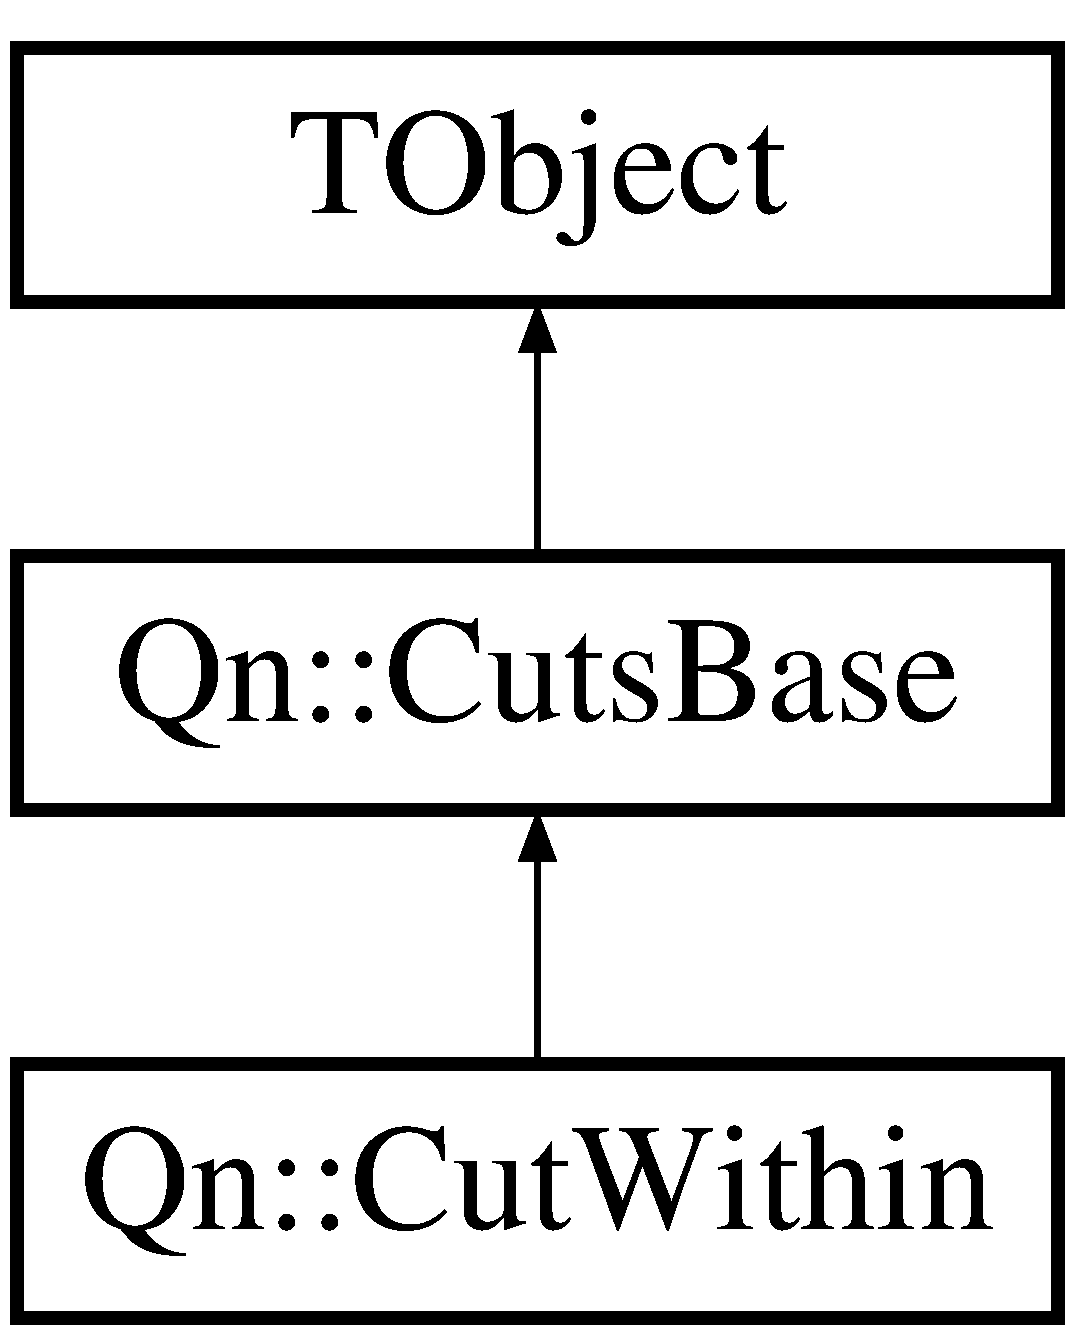
\includegraphics[height=3.000000cm]{classQn_1_1CutWithin}
\end{center}
\end{figure}
\subsection*{Public Member Functions}
\begin{DoxyCompactItemize}
\item 
\mbox{\Hypertarget{classQn_1_1CutWithin_aff81a10abb3c7f00c2c4b5868e8a1da5}\label{classQn_1_1CutWithin_aff81a10abb3c7f00c2c4b5868e8a1da5}} 
\mbox{\hyperlink{classQn_1_1CutWithin_aff81a10abb3c7f00c2c4b5868e8a1da5}{Cut\+Within}} ()
\begin{DoxyCompactList}\small\item\em Default constructor. \end{DoxyCompactList}\item 
\mbox{\hyperlink{classQn_1_1CutWithin_a49442a5fdc7b6bfce9818c2c99b859ce}{Cut\+Within}} (const \mbox{\hyperlink{classQn_1_1CutWithin}{Cut\+Within}} \&cut)
\item 
\mbox{\hyperlink{classQn_1_1CutWithin_a8f151a39deb135d441907394c9a9ad17}{Cut\+Within}} (Int\+\_\+t var\+Id, Float\+\_\+t min, Float\+\_\+t max)
\item 
\mbox{\Hypertarget{classQn_1_1CutWithin_a5f1264641e321d065b4dc4f68aec8ff8}\label{classQn_1_1CutWithin_a5f1264641e321d065b4dc4f68aec8ff8}} 
virtual \mbox{\hyperlink{classQn_1_1CutWithin_a5f1264641e321d065b4dc4f68aec8ff8}{$\sim$\+Cut\+Within}} ()
\begin{DoxyCompactList}\small\item\em Default destructor. Does nothing. \end{DoxyCompactList}\item 
virtual Bool\+\_\+t \mbox{\hyperlink{classQn_1_1CutWithin_a0766a4ec99389a9991ee8f2c974bdaf4}{Is\+Selected}} (const double $\ast$variable\+Container)
\end{DoxyCompactItemize}
\subsection*{Additional Inherited Members}


\subsection{Constructor \& Destructor Documentation}
\mbox{\Hypertarget{classQn_1_1CutWithin_a49442a5fdc7b6bfce9818c2c99b859ce}\label{classQn_1_1CutWithin_a49442a5fdc7b6bfce9818c2c99b859ce}} 
\index{Qn\+::\+Cut\+Within@{Qn\+::\+Cut\+Within}!Cut\+Within@{Cut\+Within}}
\index{Cut\+Within@{Cut\+Within}!Qn\+::\+Cut\+Within@{Qn\+::\+Cut\+Within}}
\subsubsection{\texorpdfstring{Cut\+Within()}{CutWithin()}\hspace{0.1cm}{\footnotesize\ttfamily [1/2]}}
{\footnotesize\ttfamily Qn\+::\+Cut\+Within\+::\+Cut\+Within (\begin{DoxyParamCaption}\item[{const \mbox{\hyperlink{classQn_1_1CutWithin}{Cut\+Within}} \&}]{cut }\end{DoxyParamCaption})}

Copy constructor 
\begin{DoxyParams}{Parameters}
{\em cut} & the cut object to be cloned \\
\hline
\end{DoxyParams}
\mbox{\Hypertarget{classQn_1_1CutWithin_a8f151a39deb135d441907394c9a9ad17}\label{classQn_1_1CutWithin_a8f151a39deb135d441907394c9a9ad17}} 
\index{Qn\+::\+Cut\+Within@{Qn\+::\+Cut\+Within}!Cut\+Within@{Cut\+Within}}
\index{Cut\+Within@{Cut\+Within}!Qn\+::\+Cut\+Within@{Qn\+::\+Cut\+Within}}
\subsubsection{\texorpdfstring{Cut\+Within()}{CutWithin()}\hspace{0.1cm}{\footnotesize\ttfamily [2/2]}}
{\footnotesize\ttfamily Qn\+::\+Cut\+Within\+::\+Cut\+Within (\begin{DoxyParamCaption}\item[{Int\+\_\+t}]{var\+Id,  }\item[{Float\+\_\+t}]{min,  }\item[{Float\+\_\+t}]{max }\end{DoxyParamCaption})}

Normal constructor 
\begin{DoxyParams}{Parameters}
{\em var\+Id} & external Id for the affected variable \\
\hline
{\em min} & the value the variable content should be above \\
\hline
{\em max} & the value the variable content should be below \\
\hline
\end{DoxyParams}


\subsection{Member Function Documentation}
\mbox{\Hypertarget{classQn_1_1CutWithin_a0766a4ec99389a9991ee8f2c974bdaf4}\label{classQn_1_1CutWithin_a0766a4ec99389a9991ee8f2c974bdaf4}} 
\index{Qn\+::\+Cut\+Within@{Qn\+::\+Cut\+Within}!Is\+Selected@{Is\+Selected}}
\index{Is\+Selected@{Is\+Selected}!Qn\+::\+Cut\+Within@{Qn\+::\+Cut\+Within}}
\subsubsection{\texorpdfstring{Is\+Selected()}{IsSelected()}}
{\footnotesize\ttfamily Bool\+\_\+t Qn\+::\+Cut\+Within\+::\+Is\+Selected (\begin{DoxyParamCaption}\item[{const double $\ast$}]{variable\+Container }\end{DoxyParamCaption})\hspace{0.3cm}{\ttfamily [inline]}, {\ttfamily [virtual]}}

Check if the actual variable value passes the cut


\begin{DoxyParams}{Parameters}
{\em variable\+Container} & the current variables content addressed by var Id \\
\hline
\end{DoxyParams}
\begin{DoxyReturn}{Returns}
k\+T\+R\+UE if the actual value is below the threshold else k\+F\+A\+L\+SE 
\end{DoxyReturn}


Implements \mbox{\hyperlink{classQn_1_1CutsBase_aab081fa4220144505ca838539d83aa8d}{Qn\+::\+Cuts\+Base}}.



The documentation for this class was generated from the following files\+:\begin{DoxyCompactItemize}
\item 
D\+T\+\_\+\+Flow/\+Qn\+Corrections/include/Cut\+Within.\+h\item 
D\+T\+\_\+\+Flow/\+Qn\+Corrections/Cut\+Within.\+cpp\end{DoxyCompactItemize}

\hypertarget{classQn_1_1DataContainer}{}\section{Qn\+:\+:Data\+Container$<$ T $>$ Class Template Reference}
\label{classQn_1_1DataContainer}\index{Qn\+::\+Data\+Container$<$ T $>$@{Qn\+::\+Data\+Container$<$ T $>$}}


Template container class for Q-\/vectors and correlations.  




{\ttfamily \#include $<$Data\+Container.\+h$>$}

Inheritance diagram for Qn\+:\+:Data\+Container$<$ T $>$\+:\begin{figure}[H]
\begin{center}
\leavevmode
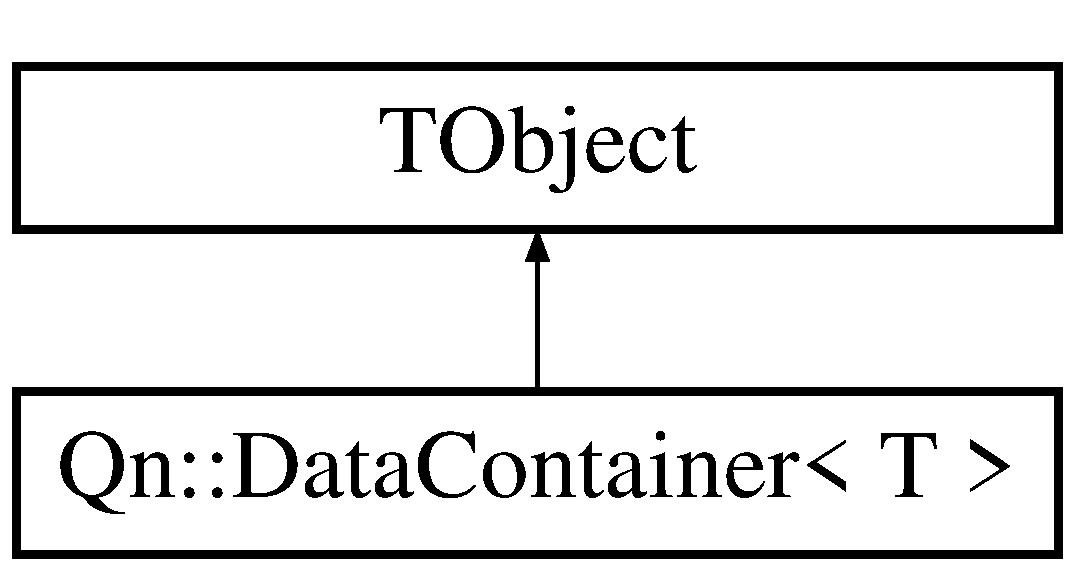
\includegraphics[height=2.000000cm]{classQn_1_1DataContainer}
\end{center}
\end{figure}
\subsection*{Public Types}
\begin{DoxyCompactItemize}
\item 
\mbox{\Hypertarget{classQn_1_1DataContainer_a5a4ec4b1dad17823d08521e87bb82d80}\label{classQn_1_1DataContainer_a5a4ec4b1dad17823d08521e87bb82d80}} 
enum {\bfseries Settings} \{ {\bfseries Is\+Mergable} = B\+IT(14), 
{\bfseries N\+Central\+Settings} = B\+IT(15)
 \}
\item 
\mbox{\Hypertarget{classQn_1_1DataContainer_ada8edb56cdc0396c0221600a29a19b15}\label{classQn_1_1DataContainer_ada8edb56cdc0396c0221600a29a19b15}} 
using {\bfseries Qn\+Axes} = std\+::vector$<$ \mbox{\hyperlink{classQn_1_1Axis}{Axis}} $>$
\item 
\mbox{\Hypertarget{classQn_1_1DataContainer_a3b96114bb9dfccb532095194bd26837c}\label{classQn_1_1DataContainer_a3b96114bb9dfccb532095194bd26837c}} 
using {\bfseries size\+\_\+type} = std\+::size\+\_\+t
\item 
\mbox{\Hypertarget{classQn_1_1DataContainer_a1cf7439f08b74652e4016d7b6586dbf1}\label{classQn_1_1DataContainer_a1cf7439f08b74652e4016d7b6586dbf1}} 
using {\bfseries iterator} = typename std\+::vector$<$ T $>$\+::iterator
\item 
\mbox{\Hypertarget{classQn_1_1DataContainer_a241d6f7b4490707b08ce0a8aa08b07a1}\label{classQn_1_1DataContainer_a241d6f7b4490707b08ce0a8aa08b07a1}} 
using {\bfseries const\+\_\+iterator} = typename std\+::vector$<$ T $>$\+::const\+\_\+iterator
\end{DoxyCompactItemize}
\subsection*{Public Member Functions}
\begin{DoxyCompactItemize}
\item 
\mbox{\hyperlink{classQn_1_1DataContainer_a5443239806a27f42e502c88d6f76328e}{Data\+Container}} ()
\item 
\mbox{\hyperlink{classQn_1_1DataContainer_a1f171432b577b5d0061908d461c39198}{Data\+Container}} (std\+::vector$<$ \mbox{\hyperlink{classQn_1_1Axis}{Axis}} $>$ axes)
\item 
\mbox{\Hypertarget{classQn_1_1DataContainer_a92dd60f02cc0f05d0c06ca95d68b3551}\label{classQn_1_1DataContainer_a92dd60f02cc0f05d0c06ca95d68b3551}} 
const\+\_\+iterator \mbox{\hyperlink{classQn_1_1DataContainer_a92dd60f02cc0f05d0c06ca95d68b3551}{begin}} () const
\begin{DoxyCompactList}\small\item\em iterator for external use \end{DoxyCompactList}\item 
\mbox{\Hypertarget{classQn_1_1DataContainer_a8ea9e17c117d88252bee513bed2208b6}\label{classQn_1_1DataContainer_a8ea9e17c117d88252bee513bed2208b6}} 
const\+\_\+iterator \mbox{\hyperlink{classQn_1_1DataContainer_a8ea9e17c117d88252bee513bed2208b6}{end}} () const
\begin{DoxyCompactList}\small\item\em iterator for external use \end{DoxyCompactList}\item 
\mbox{\Hypertarget{classQn_1_1DataContainer_ad9d4fa0d39d72c3e5cbf527c9b462322}\label{classQn_1_1DataContainer_ad9d4fa0d39d72c3e5cbf527c9b462322}} 
iterator \mbox{\hyperlink{classQn_1_1DataContainer_ad9d4fa0d39d72c3e5cbf527c9b462322}{begin}} ()
\begin{DoxyCompactList}\small\item\em iterator for external use \end{DoxyCompactList}\item 
\mbox{\Hypertarget{classQn_1_1DataContainer_aaab2056ff13b5342a5dc9a94ca6e9141}\label{classQn_1_1DataContainer_aaab2056ff13b5342a5dc9a94ca6e9141}} 
iterator \mbox{\hyperlink{classQn_1_1DataContainer_aaab2056ff13b5342a5dc9a94ca6e9141}{end}} ()
\begin{DoxyCompactList}\small\item\em iterator for external use \end{DoxyCompactList}\item 
size\+\_\+type \mbox{\hyperlink{classQn_1_1DataContainer_a95370695e706347db87491cdd65fcffb}{size}} () const noexcept
\item 
void \mbox{\hyperlink{classQn_1_1DataContainer_a1e60f7b54d499b8bca9ea2a04fc55340}{Add\+Axes}} (const Qn\+Axes \&axes)
\item 
void \mbox{\hyperlink{classQn_1_1DataContainer_a5fd9996f60f536d991b0b4f6cdd9d838}{Add\+Axis}} (const \mbox{\hyperlink{classQn_1_1Axis}{Axis}} \&axis)
\item 
void \mbox{\hyperlink{classQn_1_1DataContainer_a2baf9c75f0652ea0a0ef30aaf2ce8deb}{Initialize\+Entries}} (const T obj)
\item 
std\+::vector$<$ size\+\_\+type $>$ \mbox{\hyperlink{classQn_1_1DataContainer_a5acec0ed294b3225f32981636af698d7}{Get\+Diagonal}} (const Qn\+Axes \&axes)
\item 
T const  \& \mbox{\hyperlink{classQn_1_1DataContainer_a637662b4443d60c9aab35a906ee98877}{At}} (const typename std\+::vector$<$ size\+\_\+type $>$ \&bins) const
\item 
T \& \mbox{\hyperlink{classQn_1_1DataContainer_af1565f4febc1125cac6e1fed8398f38f}{At}} (const typename std\+::vector$<$ size\+\_\+type $>$ \&bins)
\item 
T \& \mbox{\hyperlink{classQn_1_1DataContainer_a929706074edc9dd3bcc89a68c307b9c3}{At}} (size\+\_\+type index) noexcept
\item 
T const  \& \mbox{\hyperlink{classQn_1_1DataContainer_af89617f2b9005713df9134dbd8417835}{At}} (size\+\_\+type index) const noexcept
\item 
{\footnotesize template$<$typename Function $>$ }\\void \mbox{\hyperlink{classQn_1_1DataContainer_a617cf83f205e54105a339e819592daf0}{Call\+On\+Element}} (const typename std\+::vector$<$ size\+\_\+type $>$ \&indices, Function \&\&lambda)
\item 
{\footnotesize template$<$typename Function $>$ }\\void \mbox{\hyperlink{classQn_1_1DataContainer_a1fa55b9f9adc8a07b3a4d7ed51b5516b}{Call\+On\+Element}} (Function \&\&lambda)
\item 
{\footnotesize template$<$typename Function $>$ }\\void \mbox{\hyperlink{classQn_1_1DataContainer_af663740b50d50356b29149e0d013d40d}{Call\+On\+Element}} (const std\+::vector$<$ float $>$ \&coordinates, Function \&\&lambda)
\item 
{\footnotesize template$<$typename Function $>$ }\\void \mbox{\hyperlink{classQn_1_1DataContainer_ad98f8acd6c4ac7f5ba171eb779acbcee}{Call\+On\+Element}} (const long index, Function \&\&lambda)
\item 
const Qn\+Axes \& \mbox{\hyperlink{classQn_1_1DataContainer_a8c603692b39277e0cfbaa83c69c31336}{Get\+Axes}} () const
\item 
Qn\+Axes \& \mbox{\hyperlink{classQn_1_1DataContainer_acf5507cd4e2b1cb26b58b176b9a7cde3}{Get\+Axes}} ()
\item 
\mbox{\hyperlink{classQn_1_1Axis}{Axis}} \mbox{\hyperlink{classQn_1_1DataContainer_a1fdc10d4a7feb391aa7291900c9e2073}{Get\+Axis}} (const std\+::string name) const
\item 
void \mbox{\hyperlink{classQn_1_1DataContainer_ac4cb2d0af4e28966603b97dc50e5ce50}{Get\+Index}} (std\+::vector$<$ size\+\_\+type $>$ \&indices, const unsigned long offset) const
\item 
std\+::vector$<$ size\+\_\+type $>$ \mbox{\hyperlink{classQn_1_1DataContainer_aa9b5b94b254a2e447b843b3bed6a9b92}{Get\+Index}} (const unsigned long offset) const
\item 
std\+::string \mbox{\hyperlink{classQn_1_1DataContainer_a50ede53a78fd13dfa1cf4bad0b04babc}{Get\+Bin\+Description}} (const unsigned long offset) const
\item 
{\footnotesize template$<$typename Function $>$ }\\\mbox{\hyperlink{classQn_1_1DataContainer}{Data\+Container}}$<$ T $>$ \mbox{\hyperlink{classQn_1_1DataContainer_ac20e9292be55e0241647f356c1d7bb4e}{Projection}} (const std\+::vector$<$ std\+::string $>$ axis\+\_\+names, Function \&\&lambda) const
\item 
\mbox{\hyperlink{classQn_1_1DataContainer}{Data\+Container}}$<$ T $>$ \mbox{\hyperlink{classQn_1_1DataContainer_a0f0c2dbb7e48d706ca19d45fa32f99f4}{Projection}} (const std\+::vector$<$ std\+::string $>$ axis\+\_\+names=\{\}) const
\item 
{\footnotesize template$<$typename Function $>$ }\\\mbox{\hyperlink{classQn_1_1DataContainer}{Data\+Container}}$<$ T $>$ \mbox{\hyperlink{classQn_1_1DataContainer_a40c7b7ffaa61bbf616006b2fa95f6d5f}{Projection\+Exclude}} (const std\+::vector$<$ std\+::string $>$ axis\+\_\+names, Function \&\&lambda, std\+::vector$<$ int $>$ exindices) const
\item 
{\footnotesize template$<$typename Function $>$ }\\\mbox{\hyperlink{classQn_1_1DataContainer}{Data\+Container}}$<$ T $>$ \mbox{\hyperlink{classQn_1_1DataContainer_a270d35d401e506983516dbd00728232d}{Map}} (Function \&\&lambda) const
\item 
\mbox{\hyperlink{classQn_1_1DataContainer}{Data\+Container}}$<$ T $>$ \mbox{\hyperlink{classQn_1_1DataContainer_a6f6590866c0cfe451cf966292d3eb69a}{Select}} (const \mbox{\hyperlink{classQn_1_1Axis}{Axis}} \&axis) const
\item 
{\footnotesize template$<$typename Function $>$ }\\\mbox{\hyperlink{classQn_1_1DataContainer}{Data\+Container}}$<$ T $>$ \mbox{\hyperlink{classQn_1_1DataContainer_aeac968c52250853cca2fd0ed2978c8e4}{Rebin}} (const \mbox{\hyperlink{classQn_1_1Axis}{Axis}} \&rebinaxis, Function \&\&lambda) const
\item 
\mbox{\hyperlink{classQn_1_1DataContainer}{Data\+Container}}$<$ T $>$ \mbox{\hyperlink{classQn_1_1DataContainer_a775225cf7b6e9bd66c7571531013c07d}{Rebin}} (const \mbox{\hyperlink{classQn_1_1Axis}{Axis}} \&rebinaxis) const
\item 
{\footnotesize template$<$typename Function $>$ }\\\mbox{\hyperlink{classQn_1_1DataContainer}{Data\+Container}}$<$ T $>$ \mbox{\hyperlink{classQn_1_1DataContainer_a2c165924fca1953fd09f2a7aabdb608c}{Filter}} (Function \&\&lambda) const
\item 
{\footnotesize template$<$typename Function $>$ }\\\mbox{\hyperlink{classQn_1_1DataContainer}{Data\+Container}}$<$ T $>$ \mbox{\hyperlink{classQn_1_1DataContainer_afe0598569174690569116e5120234b7d}{Apply}} (const \mbox{\hyperlink{classQn_1_1DataContainer}{Data\+Container}}$<$ T $>$ \&data, Function \&\&lambda) const
\item 
void \mbox{\hyperlink{classQn_1_1DataContainer_acd8c7e0e00f681929bf29f35830ff232}{Clear\+Data}} ()
\item 
void \mbox{\hyperlink{classQn_1_1DataContainer_a60a01024cc3b7c421ff1270608975ee7}{Clear\+Data\+At}} (const size\+\_\+type position)
\item 
bool \mbox{\hyperlink{classQn_1_1DataContainer_a5cb38267726d0c1e2196f51d066e306f}{Is\+Integrated}} () const
\item 
Long64\+\_\+t \mbox{\hyperlink{classQn_1_1DataContainer_a7bc5a8330ed6a0a1964fc27af7fd6775}{Merge}} (T\+Collection $\ast$inputlist)
\item 
void \mbox{\hyperlink{classQn_1_1DataContainer_a655e42708d02b905b28cba7fb4f0dd42}{Set\+Setting}} (unsigned int bits)
\item 
\mbox{\Hypertarget{classQn_1_1DataContainer_a18f35066b8d8519b827256ddd6971921}\label{classQn_1_1DataContainer_a18f35066b8d8519b827256ddd6971921}} 
void {\bfseries Reset\+Setting} (unsigned int bits)
\item 
void \mbox{\hyperlink{classQn_1_1DataContainer_a146d918368c9ab5273e223fac3bcedf1}{N\+Draw}} (Option\+\_\+t $\ast$option, const std\+::string \&axis\+\_\+name=\char`\"{}\char`\"{})
\item 
virtual void \mbox{\hyperlink{classQn_1_1DataContainer_acb108bdec1e5d316e0b8504546a961c4}{Browse}} (T\+Browser $\ast$b)
\item 
\mbox{\Hypertarget{classQn_1_1DataContainer_aab04c45c30d45f97b0d14fdf77b7e027}\label{classQn_1_1DataContainer_aab04c45c30d45f97b0d14fdf77b7e027}} 
{\footnotesize template$<$$>$ }\\void {\bfseries Browse} (T\+Browser $\ast$b)
\item 
\mbox{\Hypertarget{classQn_1_1DataContainer_aa4a6b4892e6f6355e4eccc3676fb0398}\label{classQn_1_1DataContainer_aa4a6b4892e6f6355e4eccc3676fb0398}} 
{\footnotesize template$<$$>$ }\\void {\bfseries Browse} (T\+Browser $\ast$b)
\item 
\mbox{\Hypertarget{classQn_1_1DataContainer_a66d138be93bbaed9617de46d0cb32505}\label{classQn_1_1DataContainer_a66d138be93bbaed9617de46d0cb32505}} 
{\footnotesize template$<$$>$ }\\void {\bfseries N\+Draw} (Option\+\_\+t $\ast$option, const std\+::string \&axis\+\_\+name)
\item 
\mbox{\Hypertarget{classQn_1_1DataContainer_a33c502bca3a71804831f2a1dff0951b0}\label{classQn_1_1DataContainer_a33c502bca3a71804831f2a1dff0951b0}} 
{\footnotesize template$<$$>$ }\\void {\bfseries Set\+Setting} (const unsigned int bits)
\item 
\mbox{\Hypertarget{classQn_1_1DataContainer_ab9bb103e9b8ecded19d30979809b08a3}\label{classQn_1_1DataContainer_ab9bb103e9b8ecded19d30979809b08a3}} 
{\footnotesize template$<$$>$ }\\void {\bfseries Reset\+Setting} (const unsigned int bits)
\item 
\mbox{\Hypertarget{classQn_1_1DataContainer_a823ec9f69fcbbd4af4b31d8866806c25}\label{classQn_1_1DataContainer_a823ec9f69fcbbd4af4b31d8866806c25}} 
{\footnotesize template$<$$>$ }\\Long64\+\_\+t {\bfseries Merge} (T\+Collection $\ast$inputlist)=delete
\item 
\mbox{\Hypertarget{classQn_1_1DataContainer_a76da5955d2884b691edd5afce6d3a531}\label{classQn_1_1DataContainer_a76da5955d2884b691edd5afce6d3a531}} 
{\footnotesize template$<$$>$ }\\Long64\+\_\+t {\bfseries Merge} (T\+Collection $\ast$inputlist)=delete
\item 
\mbox{\Hypertarget{classQn_1_1DataContainer_a2fe2338539953479112cd96155b3bbd8}\label{classQn_1_1DataContainer_a2fe2338539953479112cd96155b3bbd8}} 
{\footnotesize template$<$$>$ }\\Long64\+\_\+t {\bfseries Merge} (T\+Collection $\ast$inputlist)=delete
\item 
\mbox{\Hypertarget{classQn_1_1DataContainer_acce1b182d0c927793f12625b17a9666b}\label{classQn_1_1DataContainer_acce1b182d0c927793f12625b17a9666b}} 
{\footnotesize template$<$$>$ }\\Long64\+\_\+t {\bfseries Merge} (T\+Collection $\ast$inputlist)=delete
\end{DoxyCompactItemize}


\subsection{Detailed Description}
\subsubsection*{template$<$typename T$>$\newline
class Qn\+::\+Data\+Container$<$ T $>$}

Template container class for Q-\/vectors and correlations. 


\begin{DoxyParams}{Parameters}
{\em T} & Type of object inside of container \\
\hline
\end{DoxyParams}


\subsection{Constructor \& Destructor Documentation}
\mbox{\Hypertarget{classQn_1_1DataContainer_a5443239806a27f42e502c88d6f76328e}\label{classQn_1_1DataContainer_a5443239806a27f42e502c88d6f76328e}} 
\index{Qn\+::\+Data\+Container@{Qn\+::\+Data\+Container}!Data\+Container@{Data\+Container}}
\index{Data\+Container@{Data\+Container}!Qn\+::\+Data\+Container@{Qn\+::\+Data\+Container}}
\subsubsection{\texorpdfstring{Data\+Container()}{DataContainer()}\hspace{0.1cm}{\footnotesize\ttfamily [1/2]}}
{\footnotesize\ttfamily template$<$typename T$>$ \\
\mbox{\hyperlink{classQn_1_1DataContainer}{Qn\+::\+Data\+Container}}$<$ T $>$\+::\mbox{\hyperlink{classQn_1_1DataContainer}{Data\+Container}} (\begin{DoxyParamCaption}{ }\end{DoxyParamCaption})\hspace{0.3cm}{\ttfamily [inline]}}

Default constructor Axes can be added later. If no axes are added the \mbox{\hyperlink{classQn_1_1DataContainer}{Data\+Container}} is integrated with only one entry. \mbox{\Hypertarget{classQn_1_1DataContainer_a1f171432b577b5d0061908d461c39198}\label{classQn_1_1DataContainer_a1f171432b577b5d0061908d461c39198}} 
\index{Qn\+::\+Data\+Container@{Qn\+::\+Data\+Container}!Data\+Container@{Data\+Container}}
\index{Data\+Container@{Data\+Container}!Qn\+::\+Data\+Container@{Qn\+::\+Data\+Container}}
\subsubsection{\texorpdfstring{Data\+Container()}{DataContainer()}\hspace{0.1cm}{\footnotesize\ttfamily [2/2]}}
{\footnotesize\ttfamily template$<$typename T$>$ \\
\mbox{\hyperlink{classQn_1_1DataContainer}{Qn\+::\+Data\+Container}}$<$ T $>$\+::\mbox{\hyperlink{classQn_1_1DataContainer}{Data\+Container}} (\begin{DoxyParamCaption}\item[{std\+::vector$<$ \mbox{\hyperlink{classQn_1_1Axis}{Axis}} $>$}]{axes }\end{DoxyParamCaption})\hspace{0.3cm}{\ttfamily [inline]}, {\ttfamily [explicit]}}

Constructor 
\begin{DoxyParams}{Parameters}
{\em axes} & vector of axes of the datacontainer. \\
\hline
\end{DoxyParams}


\subsection{Member Function Documentation}
\mbox{\Hypertarget{classQn_1_1DataContainer_a1e60f7b54d499b8bca9ea2a04fc55340}\label{classQn_1_1DataContainer_a1e60f7b54d499b8bca9ea2a04fc55340}} 
\index{Qn\+::\+Data\+Container@{Qn\+::\+Data\+Container}!Add\+Axes@{Add\+Axes}}
\index{Add\+Axes@{Add\+Axes}!Qn\+::\+Data\+Container@{Qn\+::\+Data\+Container}}
\subsubsection{\texorpdfstring{Add\+Axes()}{AddAxes()}}
{\footnotesize\ttfamily template$<$typename T$>$ \\
void \mbox{\hyperlink{classQn_1_1DataContainer}{Qn\+::\+Data\+Container}}$<$ T $>$\+::Add\+Axes (\begin{DoxyParamCaption}\item[{const Qn\+Axes \&}]{axes }\end{DoxyParamCaption})\hspace{0.3cm}{\ttfamily [inline]}}

Adds axes for storing data 
\begin{DoxyParams}{Parameters}
{\em axes} & vector of axes \\
\hline
\end{DoxyParams}
\mbox{\Hypertarget{classQn_1_1DataContainer_a5fd9996f60f536d991b0b4f6cdd9d838}\label{classQn_1_1DataContainer_a5fd9996f60f536d991b0b4f6cdd9d838}} 
\index{Qn\+::\+Data\+Container@{Qn\+::\+Data\+Container}!Add\+Axis@{Add\+Axis}}
\index{Add\+Axis@{Add\+Axis}!Qn\+::\+Data\+Container@{Qn\+::\+Data\+Container}}
\subsubsection{\texorpdfstring{Add\+Axis()}{AddAxis()}}
{\footnotesize\ttfamily template$<$typename T$>$ \\
void \mbox{\hyperlink{classQn_1_1DataContainer}{Qn\+::\+Data\+Container}}$<$ T $>$\+::Add\+Axis (\begin{DoxyParamCaption}\item[{const \mbox{\hyperlink{classQn_1_1Axis}{Axis}} \&}]{axis }\end{DoxyParamCaption})\hspace{0.3cm}{\ttfamily [inline]}}

Adds existing axis for storing the data with variable binning 
\begin{DoxyParams}{Parameters}
{\em axis} & \mbox{\hyperlink{classQn_1_1Axis}{Axis}} to be added. \\
\hline
\end{DoxyParams}
\mbox{\Hypertarget{classQn_1_1DataContainer_afe0598569174690569116e5120234b7d}\label{classQn_1_1DataContainer_afe0598569174690569116e5120234b7d}} 
\index{Qn\+::\+Data\+Container@{Qn\+::\+Data\+Container}!Apply@{Apply}}
\index{Apply@{Apply}!Qn\+::\+Data\+Container@{Qn\+::\+Data\+Container}}
\subsubsection{\texorpdfstring{Apply()}{Apply()}}
{\footnotesize\ttfamily template$<$typename T$>$ \\
template$<$typename Function $>$ \\
\mbox{\hyperlink{classQn_1_1DataContainer}{Data\+Container}}$<$T$>$ \mbox{\hyperlink{classQn_1_1DataContainer}{Qn\+::\+Data\+Container}}$<$ T $>$\+::Apply (\begin{DoxyParamCaption}\item[{const \mbox{\hyperlink{classQn_1_1DataContainer}{Data\+Container}}$<$ T $>$ \&}]{data,  }\item[{Function \&\&}]{lambda }\end{DoxyParamCaption}) const\hspace{0.3cm}{\ttfamily [inline]}}

Apply function to two datacontainers. The axes need to have the same order. Elements in datacontainer with smaller dimensions are used as \char`\"{}integrated bins\char`\"{}. 
\begin{DoxyTemplParams}{Template Parameters}
{\em Function} & type of function \\
\hline
\end{DoxyTemplParams}

\begin{DoxyParams}{Parameters}
{\em data} & Datacontainer \\
\hline
{\em lambda} & function to be applied on both elements \\
\hline
\end{DoxyParams}
\begin{DoxyReturn}{Returns}
resulting datacontainer. 
\end{DoxyReturn}
\mbox{\Hypertarget{classQn_1_1DataContainer_a637662b4443d60c9aab35a906ee98877}\label{classQn_1_1DataContainer_a637662b4443d60c9aab35a906ee98877}} 
\index{Qn\+::\+Data\+Container@{Qn\+::\+Data\+Container}!At@{At}}
\index{At@{At}!Qn\+::\+Data\+Container@{Qn\+::\+Data\+Container}}
\subsubsection{\texorpdfstring{At()}{At()}\hspace{0.1cm}{\footnotesize\ttfamily [1/4]}}
{\footnotesize\ttfamily template$<$typename T$>$ \\
T const\& \mbox{\hyperlink{classQn_1_1DataContainer}{Qn\+::\+Data\+Container}}$<$ T $>$\+::At (\begin{DoxyParamCaption}\item[{const typename std\+::vector$<$ size\+\_\+type $>$ \&}]{bins }\end{DoxyParamCaption}) const\hspace{0.3cm}{\ttfamily [inline]}}

Get element in the specified bin 
\begin{DoxyParams}{Parameters}
{\em bins} & Vector of bin indices of the desired element \\
\hline
\end{DoxyParams}
\begin{DoxyReturn}{Returns}
Element 
\end{DoxyReturn}
\mbox{\Hypertarget{classQn_1_1DataContainer_af1565f4febc1125cac6e1fed8398f38f}\label{classQn_1_1DataContainer_af1565f4febc1125cac6e1fed8398f38f}} 
\index{Qn\+::\+Data\+Container@{Qn\+::\+Data\+Container}!At@{At}}
\index{At@{At}!Qn\+::\+Data\+Container@{Qn\+::\+Data\+Container}}
\subsubsection{\texorpdfstring{At()}{At()}\hspace{0.1cm}{\footnotesize\ttfamily [2/4]}}
{\footnotesize\ttfamily template$<$typename T$>$ \\
T\& \mbox{\hyperlink{classQn_1_1DataContainer}{Qn\+::\+Data\+Container}}$<$ T $>$\+::At (\begin{DoxyParamCaption}\item[{const typename std\+::vector$<$ size\+\_\+type $>$ \&}]{bins }\end{DoxyParamCaption})\hspace{0.3cm}{\ttfamily [inline]}}

Get element in the specified bin 
\begin{DoxyParams}{Parameters}
{\em bins} & Vector of bin indices of the desired element \\
\hline
\end{DoxyParams}
\begin{DoxyReturn}{Returns}
Element 
\end{DoxyReturn}
\mbox{\Hypertarget{classQn_1_1DataContainer_a929706074edc9dd3bcc89a68c307b9c3}\label{classQn_1_1DataContainer_a929706074edc9dd3bcc89a68c307b9c3}} 
\index{Qn\+::\+Data\+Container@{Qn\+::\+Data\+Container}!At@{At}}
\index{At@{At}!Qn\+::\+Data\+Container@{Qn\+::\+Data\+Container}}
\subsubsection{\texorpdfstring{At()}{At()}\hspace{0.1cm}{\footnotesize\ttfamily [3/4]}}
{\footnotesize\ttfamily template$<$typename T$>$ \\
T\& \mbox{\hyperlink{classQn_1_1DataContainer}{Qn\+::\+Data\+Container}}$<$ T $>$\+::At (\begin{DoxyParamCaption}\item[{size\+\_\+type}]{index }\end{DoxyParamCaption})\hspace{0.3cm}{\ttfamily [inline]}, {\ttfamily [noexcept]}}

Get element in the specified bin 
\begin{DoxyParams}{Parameters}
{\em index} & index of element \\
\hline
\end{DoxyParams}
\begin{DoxyReturn}{Returns}
Element 
\end{DoxyReturn}
\mbox{\Hypertarget{classQn_1_1DataContainer_af89617f2b9005713df9134dbd8417835}\label{classQn_1_1DataContainer_af89617f2b9005713df9134dbd8417835}} 
\index{Qn\+::\+Data\+Container@{Qn\+::\+Data\+Container}!At@{At}}
\index{At@{At}!Qn\+::\+Data\+Container@{Qn\+::\+Data\+Container}}
\subsubsection{\texorpdfstring{At()}{At()}\hspace{0.1cm}{\footnotesize\ttfamily [4/4]}}
{\footnotesize\ttfamily template$<$typename T$>$ \\
T const\& \mbox{\hyperlink{classQn_1_1DataContainer}{Qn\+::\+Data\+Container}}$<$ T $>$\+::At (\begin{DoxyParamCaption}\item[{size\+\_\+type}]{index }\end{DoxyParamCaption}) const\hspace{0.3cm}{\ttfamily [inline]}, {\ttfamily [noexcept]}}

Get element in the specified bin 
\begin{DoxyParams}{Parameters}
{\em index} & index of element \\
\hline
\end{DoxyParams}
\begin{DoxyReturn}{Returns}
Element 
\end{DoxyReturn}
\mbox{\Hypertarget{classQn_1_1DataContainer_acb108bdec1e5d316e0b8504546a961c4}\label{classQn_1_1DataContainer_acb108bdec1e5d316e0b8504546a961c4}} 
\index{Qn\+::\+Data\+Container@{Qn\+::\+Data\+Container}!Browse@{Browse}}
\index{Browse@{Browse}!Qn\+::\+Data\+Container@{Qn\+::\+Data\+Container}}
\subsubsection{\texorpdfstring{Browse()}{Browse()}}
{\footnotesize\ttfamily template$<$typename T$>$ \\
virtual void \mbox{\hyperlink{classQn_1_1DataContainer}{Qn\+::\+Data\+Container}}$<$ T $>$\+::Browse (\begin{DoxyParamCaption}\item[{T\+Browser $\ast$}]{b }\end{DoxyParamCaption})\hspace{0.3cm}{\ttfamily [inline]}, {\ttfamily [virtual]}}

Display contents of \mbox{\hyperlink{classQn_1_1DataContainer}{Data\+Container}} in T\+Browser. Implementation for template specializations please see below. 
\begin{DoxyParams}{Parameters}
{\em b} & T\+Browser \\
\hline
\end{DoxyParams}
\mbox{\Hypertarget{classQn_1_1DataContainer_a617cf83f205e54105a339e819592daf0}\label{classQn_1_1DataContainer_a617cf83f205e54105a339e819592daf0}} 
\index{Qn\+::\+Data\+Container@{Qn\+::\+Data\+Container}!Call\+On\+Element@{Call\+On\+Element}}
\index{Call\+On\+Element@{Call\+On\+Element}!Qn\+::\+Data\+Container@{Qn\+::\+Data\+Container}}
\subsubsection{\texorpdfstring{Call\+On\+Element()}{CallOnElement()}\hspace{0.1cm}{\footnotesize\ttfamily [1/4]}}
{\footnotesize\ttfamily template$<$typename T$>$ \\
template$<$typename Function $>$ \\
void \mbox{\hyperlink{classQn_1_1DataContainer}{Qn\+::\+Data\+Container}}$<$ T $>$\+::Call\+On\+Element (\begin{DoxyParamCaption}\item[{const typename std\+::vector$<$ size\+\_\+type $>$ \&}]{indices,  }\item[{Function \&\&}]{lambda }\end{DoxyParamCaption})\hspace{0.3cm}{\ttfamily [inline]}}

Calls function on element specified by indices. 
\begin{DoxyTemplParams}{Template Parameters}
{\em Function} & type of function to be called on the object \\
\hline
\end{DoxyTemplParams}

\begin{DoxyParams}{Parameters}
{\em indices} & indicies multidimensional indices of the element. \\
\hline
{\em lambda} & function to be called on the element. Takes element of type T as an argument. \\
\hline
\end{DoxyParams}
\mbox{\Hypertarget{classQn_1_1DataContainer_a1fa55b9f9adc8a07b3a4d7ed51b5516b}\label{classQn_1_1DataContainer_a1fa55b9f9adc8a07b3a4d7ed51b5516b}} 
\index{Qn\+::\+Data\+Container@{Qn\+::\+Data\+Container}!Call\+On\+Element@{Call\+On\+Element}}
\index{Call\+On\+Element@{Call\+On\+Element}!Qn\+::\+Data\+Container@{Qn\+::\+Data\+Container}}
\subsubsection{\texorpdfstring{Call\+On\+Element()}{CallOnElement()}\hspace{0.1cm}{\footnotesize\ttfamily [2/4]}}
{\footnotesize\ttfamily template$<$typename T$>$ \\
template$<$typename Function $>$ \\
void \mbox{\hyperlink{classQn_1_1DataContainer}{Qn\+::\+Data\+Container}}$<$ T $>$\+::Call\+On\+Element (\begin{DoxyParamCaption}\item[{Function \&\&}]{lambda }\end{DoxyParamCaption})\hspace{0.3cm}{\ttfamily [inline]}}

Calls function on element for integrated datacontainer. 
\begin{DoxyTemplParams}{Template Parameters}
{\em Function} & type of function to be called on the object \\
\hline
\end{DoxyTemplParams}

\begin{DoxyParams}{Parameters}
{\em coordinates} & coordinates of element to be modified \\
\hline
{\em lambda} & function to be called on the element. Takes element of type T as an argument. \\
\hline
\end{DoxyParams}
\mbox{\Hypertarget{classQn_1_1DataContainer_af663740b50d50356b29149e0d013d40d}\label{classQn_1_1DataContainer_af663740b50d50356b29149e0d013d40d}} 
\index{Qn\+::\+Data\+Container@{Qn\+::\+Data\+Container}!Call\+On\+Element@{Call\+On\+Element}}
\index{Call\+On\+Element@{Call\+On\+Element}!Qn\+::\+Data\+Container@{Qn\+::\+Data\+Container}}
\subsubsection{\texorpdfstring{Call\+On\+Element()}{CallOnElement()}\hspace{0.1cm}{\footnotesize\ttfamily [3/4]}}
{\footnotesize\ttfamily template$<$typename T$>$ \\
template$<$typename Function $>$ \\
void \mbox{\hyperlink{classQn_1_1DataContainer}{Qn\+::\+Data\+Container}}$<$ T $>$\+::Call\+On\+Element (\begin{DoxyParamCaption}\item[{const std\+::vector$<$ float $>$ \&}]{coordinates,  }\item[{Function \&\&}]{lambda }\end{DoxyParamCaption})\hspace{0.3cm}{\ttfamily [inline]}}

Calls function on element specified by indices. 
\begin{DoxyTemplParams}{Template Parameters}
{\em Function} & type of function to be called on the object \\
\hline
\end{DoxyTemplParams}

\begin{DoxyParams}{Parameters}
{\em coordinates} & coordinates of element to be modified \\
\hline
{\em lambda} & function to be called on the element. Takes element of type T as an argument. \\
\hline
\end{DoxyParams}
\mbox{\Hypertarget{classQn_1_1DataContainer_ad98f8acd6c4ac7f5ba171eb779acbcee}\label{classQn_1_1DataContainer_ad98f8acd6c4ac7f5ba171eb779acbcee}} 
\index{Qn\+::\+Data\+Container@{Qn\+::\+Data\+Container}!Call\+On\+Element@{Call\+On\+Element}}
\index{Call\+On\+Element@{Call\+On\+Element}!Qn\+::\+Data\+Container@{Qn\+::\+Data\+Container}}
\subsubsection{\texorpdfstring{Call\+On\+Element()}{CallOnElement()}\hspace{0.1cm}{\footnotesize\ttfamily [4/4]}}
{\footnotesize\ttfamily template$<$typename T$>$ \\
template$<$typename Function $>$ \\
void \mbox{\hyperlink{classQn_1_1DataContainer}{Qn\+::\+Data\+Container}}$<$ T $>$\+::Call\+On\+Element (\begin{DoxyParamCaption}\item[{const long}]{index,  }\item[{Function \&\&}]{lambda }\end{DoxyParamCaption})\hspace{0.3cm}{\ttfamily [inline]}}

Calls function on element specified by indices. 
\begin{DoxyTemplParams}{Template Parameters}
{\em Function} & type of function to be called on the object \\
\hline
\end{DoxyTemplParams}

\begin{DoxyParams}{Parameters}
{\em index} & linear index of element to be modified \\
\hline
{\em lambda} & function to be called on the element. Takes element of type T as an argument. \\
\hline
\end{DoxyParams}
\mbox{\Hypertarget{classQn_1_1DataContainer_acd8c7e0e00f681929bf29f35830ff232}\label{classQn_1_1DataContainer_acd8c7e0e00f681929bf29f35830ff232}} 
\index{Qn\+::\+Data\+Container@{Qn\+::\+Data\+Container}!Clear\+Data@{Clear\+Data}}
\index{Clear\+Data@{Clear\+Data}!Qn\+::\+Data\+Container@{Qn\+::\+Data\+Container}}
\subsubsection{\texorpdfstring{Clear\+Data()}{ClearData()}}
{\footnotesize\ttfamily template$<$typename T$>$ \\
void \mbox{\hyperlink{classQn_1_1DataContainer}{Qn\+::\+Data\+Container}}$<$ T $>$\+::Clear\+Data (\begin{DoxyParamCaption}{ }\end{DoxyParamCaption})\hspace{0.3cm}{\ttfamily [inline]}}

Clears data to be filled. To be called after one event. \mbox{\Hypertarget{classQn_1_1DataContainer_a60a01024cc3b7c421ff1270608975ee7}\label{classQn_1_1DataContainer_a60a01024cc3b7c421ff1270608975ee7}} 
\index{Qn\+::\+Data\+Container@{Qn\+::\+Data\+Container}!Clear\+Data\+At@{Clear\+Data\+At}}
\index{Clear\+Data\+At@{Clear\+Data\+At}!Qn\+::\+Data\+Container@{Qn\+::\+Data\+Container}}
\subsubsection{\texorpdfstring{Clear\+Data\+At()}{ClearDataAt()}}
{\footnotesize\ttfamily template$<$typename T$>$ \\
void \mbox{\hyperlink{classQn_1_1DataContainer}{Qn\+::\+Data\+Container}}$<$ T $>$\+::Clear\+Data\+At (\begin{DoxyParamCaption}\item[{const size\+\_\+type}]{position }\end{DoxyParamCaption})\hspace{0.3cm}{\ttfamily [inline]}}

Clear data at the specified postion. 
\begin{DoxyParams}{Parameters}
{\em position} & position at which to clear the data. \\
\hline
\end{DoxyParams}
\mbox{\Hypertarget{classQn_1_1DataContainer_a2c165924fca1953fd09f2a7aabdb608c}\label{classQn_1_1DataContainer_a2c165924fca1953fd09f2a7aabdb608c}} 
\index{Qn\+::\+Data\+Container@{Qn\+::\+Data\+Container}!Filter@{Filter}}
\index{Filter@{Filter}!Qn\+::\+Data\+Container@{Qn\+::\+Data\+Container}}
\subsubsection{\texorpdfstring{Filter()}{Filter()}}
{\footnotesize\ttfamily template$<$typename T$>$ \\
template$<$typename Function $>$ \\
\mbox{\hyperlink{classQn_1_1DataContainer}{Data\+Container}}$<$T$>$ \mbox{\hyperlink{classQn_1_1DataContainer}{Qn\+::\+Data\+Container}}$<$ T $>$\+::Filter (\begin{DoxyParamCaption}\item[{Function \&\&}]{lambda }\end{DoxyParamCaption}) const\hspace{0.3cm}{\ttfamily [inline]}}

Apply cut to an axis of the datacontainer. All bins which do not pass the cut are set to 0. \mbox{\Hypertarget{classQn_1_1DataContainer_a8c603692b39277e0cfbaa83c69c31336}\label{classQn_1_1DataContainer_a8c603692b39277e0cfbaa83c69c31336}} 
\index{Qn\+::\+Data\+Container@{Qn\+::\+Data\+Container}!Get\+Axes@{Get\+Axes}}
\index{Get\+Axes@{Get\+Axes}!Qn\+::\+Data\+Container@{Qn\+::\+Data\+Container}}
\subsubsection{\texorpdfstring{Get\+Axes()}{GetAxes()}\hspace{0.1cm}{\footnotesize\ttfamily [1/2]}}
{\footnotesize\ttfamily template$<$typename T$>$ \\
const Qn\+Axes\& \mbox{\hyperlink{classQn_1_1DataContainer}{Qn\+::\+Data\+Container}}$<$ T $>$\+::Get\+Axes (\begin{DoxyParamCaption}{ }\end{DoxyParamCaption}) const\hspace{0.3cm}{\ttfamily [inline]}}

Get vector of axes \begin{DoxyReturn}{Returns}
Vector of axes 
\end{DoxyReturn}
\mbox{\Hypertarget{classQn_1_1DataContainer_acf5507cd4e2b1cb26b58b176b9a7cde3}\label{classQn_1_1DataContainer_acf5507cd4e2b1cb26b58b176b9a7cde3}} 
\index{Qn\+::\+Data\+Container@{Qn\+::\+Data\+Container}!Get\+Axes@{Get\+Axes}}
\index{Get\+Axes@{Get\+Axes}!Qn\+::\+Data\+Container@{Qn\+::\+Data\+Container}}
\subsubsection{\texorpdfstring{Get\+Axes()}{GetAxes()}\hspace{0.1cm}{\footnotesize\ttfamily [2/2]}}
{\footnotesize\ttfamily template$<$typename T$>$ \\
Qn\+Axes\& \mbox{\hyperlink{classQn_1_1DataContainer}{Qn\+::\+Data\+Container}}$<$ T $>$\+::Get\+Axes (\begin{DoxyParamCaption}{ }\end{DoxyParamCaption})\hspace{0.3cm}{\ttfamily [inline]}}

Get vector of axes \begin{DoxyReturn}{Returns}
Vector of axes 
\end{DoxyReturn}
\mbox{\Hypertarget{classQn_1_1DataContainer_a1fdc10d4a7feb391aa7291900c9e2073}\label{classQn_1_1DataContainer_a1fdc10d4a7feb391aa7291900c9e2073}} 
\index{Qn\+::\+Data\+Container@{Qn\+::\+Data\+Container}!Get\+Axis@{Get\+Axis}}
\index{Get\+Axis@{Get\+Axis}!Qn\+::\+Data\+Container@{Qn\+::\+Data\+Container}}
\subsubsection{\texorpdfstring{Get\+Axis()}{GetAxis()}}
{\footnotesize\ttfamily template$<$typename T$>$ \\
\mbox{\hyperlink{classQn_1_1Axis}{Axis}} \mbox{\hyperlink{classQn_1_1DataContainer}{Qn\+::\+Data\+Container}}$<$ T $>$\+::Get\+Axis (\begin{DoxyParamCaption}\item[{const std\+::string}]{name }\end{DoxyParamCaption}) const\hspace{0.3cm}{\ttfamily [inline]}}

Get \mbox{\hyperlink{classQn_1_1Axis}{Axis}} with the given name. Throws exception when not found. 
\begin{DoxyParams}{Parameters}
{\em name} & Name of the desired axis \\
\hline
\end{DoxyParams}
\begin{DoxyReturn}{Returns}
\mbox{\hyperlink{classQn_1_1Axis}{Axis}} 
\end{DoxyReturn}
\mbox{\Hypertarget{classQn_1_1DataContainer_a50ede53a78fd13dfa1cf4bad0b04babc}\label{classQn_1_1DataContainer_a50ede53a78fd13dfa1cf4bad0b04babc}} 
\index{Qn\+::\+Data\+Container@{Qn\+::\+Data\+Container}!Get\+Bin\+Description@{Get\+Bin\+Description}}
\index{Get\+Bin\+Description@{Get\+Bin\+Description}!Qn\+::\+Data\+Container@{Qn\+::\+Data\+Container}}
\subsubsection{\texorpdfstring{Get\+Bin\+Description()}{GetBinDescription()}}
{\footnotesize\ttfamily template$<$typename T$>$ \\
std\+::string \mbox{\hyperlink{classQn_1_1DataContainer}{Qn\+::\+Data\+Container}}$<$ T $>$\+::Get\+Bin\+Description (\begin{DoxyParamCaption}\item[{const unsigned long}]{offset }\end{DoxyParamCaption}) const\hspace{0.3cm}{\ttfamily [inline]}}

Gives description by concenating axis names with coordinates 
\begin{DoxyParams}{Parameters}
{\em offset} & linear index \\
\hline
\end{DoxyParams}
\begin{DoxyReturn}{Returns}
string with bin description 
\end{DoxyReturn}
\mbox{\Hypertarget{classQn_1_1DataContainer_a5acec0ed294b3225f32981636af698d7}\label{classQn_1_1DataContainer_a5acec0ed294b3225f32981636af698d7}} 
\index{Qn\+::\+Data\+Container@{Qn\+::\+Data\+Container}!Get\+Diagonal@{Get\+Diagonal}}
\index{Get\+Diagonal@{Get\+Diagonal}!Qn\+::\+Data\+Container@{Qn\+::\+Data\+Container}}
\subsubsection{\texorpdfstring{Get\+Diagonal()}{GetDiagonal()}}
{\footnotesize\ttfamily template$<$typename T$>$ \\
std\+::vector$<$size\+\_\+type$>$ \mbox{\hyperlink{classQn_1_1DataContainer}{Qn\+::\+Data\+Container}}$<$ T $>$\+::Get\+Diagonal (\begin{DoxyParamCaption}\item[{const Qn\+Axes \&}]{axes }\end{DoxyParamCaption})\hspace{0.3cm}{\ttfamily [inline]}}

Calculates the diagonal indices of a given number of axes. 
\begin{DoxyParams}{Parameters}
{\em axes} & vector of axes. \\
\hline
\end{DoxyParams}
\begin{DoxyReturn}{Returns}
vector of linear indices in the diagonal. 
\end{DoxyReturn}
\mbox{\Hypertarget{classQn_1_1DataContainer_ac4cb2d0af4e28966603b97dc50e5ce50}\label{classQn_1_1DataContainer_ac4cb2d0af4e28966603b97dc50e5ce50}} 
\index{Qn\+::\+Data\+Container@{Qn\+::\+Data\+Container}!Get\+Index@{Get\+Index}}
\index{Get\+Index@{Get\+Index}!Qn\+::\+Data\+Container@{Qn\+::\+Data\+Container}}
\subsubsection{\texorpdfstring{Get\+Index()}{GetIndex()}\hspace{0.1cm}{\footnotesize\ttfamily [1/2]}}
{\footnotesize\ttfamily template$<$typename T$>$ \\
void \mbox{\hyperlink{classQn_1_1DataContainer}{Qn\+::\+Data\+Container}}$<$ T $>$\+::Get\+Index (\begin{DoxyParamCaption}\item[{std\+::vector$<$ size\+\_\+type $>$ \&}]{indices,  }\item[{const unsigned long}]{offset }\end{DoxyParamCaption}) const\hspace{0.3cm}{\ttfamily [inline]}}

Calculates indices in multiple dimensions from linearized index 
\begin{DoxyParams}{Parameters}
{\em indices} & Outparameter for the indices \\
\hline
{\em offset} & Index of linearized vector \\
\hline
\end{DoxyParams}
\mbox{\Hypertarget{classQn_1_1DataContainer_aa9b5b94b254a2e447b843b3bed6a9b92}\label{classQn_1_1DataContainer_aa9b5b94b254a2e447b843b3bed6a9b92}} 
\index{Qn\+::\+Data\+Container@{Qn\+::\+Data\+Container}!Get\+Index@{Get\+Index}}
\index{Get\+Index@{Get\+Index}!Qn\+::\+Data\+Container@{Qn\+::\+Data\+Container}}
\subsubsection{\texorpdfstring{Get\+Index()}{GetIndex()}\hspace{0.1cm}{\footnotesize\ttfamily [2/2]}}
{\footnotesize\ttfamily template$<$typename T$>$ \\
std\+::vector$<$size\+\_\+type$>$ \mbox{\hyperlink{classQn_1_1DataContainer}{Qn\+::\+Data\+Container}}$<$ T $>$\+::Get\+Index (\begin{DoxyParamCaption}\item[{const unsigned long}]{offset }\end{DoxyParamCaption}) const\hspace{0.3cm}{\ttfamily [inline]}}

Calculates indices in multiple dimensions from linearized index 
\begin{DoxyParams}{Parameters}
{\em offset} & Index of linearized vector \\
\hline
\end{DoxyParams}
\begin{DoxyReturn}{Returns}
vector of indices 
\end{DoxyReturn}
\mbox{\Hypertarget{classQn_1_1DataContainer_a2baf9c75f0652ea0a0ef30aaf2ce8deb}\label{classQn_1_1DataContainer_a2baf9c75f0652ea0a0ef30aaf2ce8deb}} 
\index{Qn\+::\+Data\+Container@{Qn\+::\+Data\+Container}!Initialize\+Entries@{Initialize\+Entries}}
\index{Initialize\+Entries@{Initialize\+Entries}!Qn\+::\+Data\+Container@{Qn\+::\+Data\+Container}}
\subsubsection{\texorpdfstring{Initialize\+Entries()}{InitializeEntries()}}
{\footnotesize\ttfamily template$<$typename T$>$ \\
void \mbox{\hyperlink{classQn_1_1DataContainer}{Qn\+::\+Data\+Container}}$<$ T $>$\+::Initialize\+Entries (\begin{DoxyParamCaption}\item[{const T}]{obj }\end{DoxyParamCaption})\hspace{0.3cm}{\ttfamily [inline]}}

Initialized the object in the histogram to a given object 
\begin{DoxyParams}{Parameters}
{\em obj} & Object to be intialized to \\
\hline
\end{DoxyParams}
\mbox{\Hypertarget{classQn_1_1DataContainer_a5cb38267726d0c1e2196f51d066e306f}\label{classQn_1_1DataContainer_a5cb38267726d0c1e2196f51d066e306f}} 
\index{Qn\+::\+Data\+Container@{Qn\+::\+Data\+Container}!Is\+Integrated@{Is\+Integrated}}
\index{Is\+Integrated@{Is\+Integrated}!Qn\+::\+Data\+Container@{Qn\+::\+Data\+Container}}
\subsubsection{\texorpdfstring{Is\+Integrated()}{IsIntegrated()}}
{\footnotesize\ttfamily template$<$typename T$>$ \\
bool \mbox{\hyperlink{classQn_1_1DataContainer}{Qn\+::\+Data\+Container}}$<$ T $>$\+::Is\+Integrated (\begin{DoxyParamCaption}{ }\end{DoxyParamCaption}) const\hspace{0.3cm}{\ttfamily [inline]}}

Checks if datacontainer is integrated. It is integrated if first axis is the integrated axis with Id == -\/1; \begin{DoxyReturn}{Returns}
true if integrated, else false. 
\end{DoxyReturn}
\mbox{\Hypertarget{classQn_1_1DataContainer_a270d35d401e506983516dbd00728232d}\label{classQn_1_1DataContainer_a270d35d401e506983516dbd00728232d}} 
\index{Qn\+::\+Data\+Container@{Qn\+::\+Data\+Container}!Map@{Map}}
\index{Map@{Map}!Qn\+::\+Data\+Container@{Qn\+::\+Data\+Container}}
\subsubsection{\texorpdfstring{Map()}{Map()}}
{\footnotesize\ttfamily template$<$typename T$>$ \\
template$<$typename Function $>$ \\
\mbox{\hyperlink{classQn_1_1DataContainer}{Data\+Container}}$<$T$>$ \mbox{\hyperlink{classQn_1_1DataContainer}{Qn\+::\+Data\+Container}}$<$ T $>$\+::Map (\begin{DoxyParamCaption}\item[{Function \&\&}]{lambda }\end{DoxyParamCaption}) const\hspace{0.3cm}{\ttfamily [inline]}}

Map function to datacontainer. Does not modify the original container. 
\begin{DoxyTemplParams}{Template Parameters}
{\em Function} & function \\
\hline
\end{DoxyTemplParams}

\begin{DoxyParams}{Parameters}
{\em lambda} & unary function to be applied to each element. \\
\hline
\end{DoxyParams}
\begin{DoxyReturn}{Returns}
datacontainer after applying function. 
\end{DoxyReturn}
\mbox{\Hypertarget{classQn_1_1DataContainer_a7bc5a8330ed6a0a1964fc27af7fd6775}\label{classQn_1_1DataContainer_a7bc5a8330ed6a0a1964fc27af7fd6775}} 
\index{Qn\+::\+Data\+Container@{Qn\+::\+Data\+Container}!Merge@{Merge}}
\index{Merge@{Merge}!Qn\+::\+Data\+Container@{Qn\+::\+Data\+Container}}
\subsubsection{\texorpdfstring{Merge()}{Merge()}}
{\footnotesize\ttfamily template$<$typename T$>$ \\
Long64\+\_\+t \mbox{\hyperlink{classQn_1_1DataContainer}{Qn\+::\+Data\+Container}}$<$ T $>$\+::Merge (\begin{DoxyParamCaption}\item[{T\+Collection $\ast$}]{inputlist }\end{DoxyParamCaption})\hspace{0.3cm}{\ttfamily [inline]}}

Merges \mbox{\hyperlink{classQn_1_1DataContainer}{Data\+Container}} with Data\+Containers in T\+Collection. Function used in \char`\"{}hadd\char`\"{} A function with signature T Merge( T, T) needs to be implemented for merging to work. 
\begin{DoxyParams}{Parameters}
{\em inputlist} & List of datacontainers \\
\hline
\end{DoxyParams}
\begin{DoxyReturn}{Returns}
size of datacontainer. dummyvalue 
\end{DoxyReturn}
\mbox{\Hypertarget{classQn_1_1DataContainer_a146d918368c9ab5273e223fac3bcedf1}\label{classQn_1_1DataContainer_a146d918368c9ab5273e223fac3bcedf1}} 
\index{Qn\+::\+Data\+Container@{Qn\+::\+Data\+Container}!N\+Draw@{N\+Draw}}
\index{N\+Draw@{N\+Draw}!Qn\+::\+Data\+Container@{Qn\+::\+Data\+Container}}
\subsubsection{\texorpdfstring{N\+Draw()}{NDraw()}}
{\footnotesize\ttfamily template$<$typename T$>$ \\
void \mbox{\hyperlink{classQn_1_1DataContainer}{Qn\+::\+Data\+Container}}$<$ T $>$\+::N\+Draw (\begin{DoxyParamCaption}\item[{Option\+\_\+t $\ast$}]{option,  }\item[{const std\+::string \&}]{axis\+\_\+name = {\ttfamily \char`\"{}\char`\"{}} }\end{DoxyParamCaption})\hspace{0.3cm}{\ttfamily [inline]}}

Can draw the \mbox{\hyperlink{classQn_1_1DataContainer}{Data\+Container}} with up to two dimensions. Implementration for template specializations please see below 
\begin{DoxyParams}{Parameters}
{\em option} & draw option \\
\hline
{\em axis\+\_\+name} & name of axis used for second dimension. \\
\hline
\end{DoxyParams}
\mbox{\Hypertarget{classQn_1_1DataContainer_ac20e9292be55e0241647f356c1d7bb4e}\label{classQn_1_1DataContainer_ac20e9292be55e0241647f356c1d7bb4e}} 
\index{Qn\+::\+Data\+Container@{Qn\+::\+Data\+Container}!Projection@{Projection}}
\index{Projection@{Projection}!Qn\+::\+Data\+Container@{Qn\+::\+Data\+Container}}
\subsubsection{\texorpdfstring{Projection()}{Projection()}\hspace{0.1cm}{\footnotesize\ttfamily [1/2]}}
{\footnotesize\ttfamily template$<$typename T$>$ \\
template$<$typename Function $>$ \\
\mbox{\hyperlink{classQn_1_1DataContainer}{Data\+Container}}$<$T$>$ \mbox{\hyperlink{classQn_1_1DataContainer}{Qn\+::\+Data\+Container}}$<$ T $>$\+::Projection (\begin{DoxyParamCaption}\item[{const std\+::vector$<$ std\+::string $>$}]{axis\+\_\+names,  }\item[{Function \&\&}]{lambda }\end{DoxyParamCaption}) const\hspace{0.3cm}{\ttfamily [inline]}}

Projects datacontainer on a subset of axes 
\begin{DoxyTemplParams}{Template Parameters}
{\em Function} & typename of function. \\
\hline
\end{DoxyTemplParams}

\begin{DoxyParams}{Parameters}
{\em axis\+\_\+names} & subset of axes used for the projection. \\
\hline
{\em lambda} & Function used to add two entries. \\
\hline
\end{DoxyParams}
\begin{DoxyReturn}{Returns}
projected datacontainer. 
\end{DoxyReturn}
\mbox{\Hypertarget{classQn_1_1DataContainer_a0f0c2dbb7e48d706ca19d45fa32f99f4}\label{classQn_1_1DataContainer_a0f0c2dbb7e48d706ca19d45fa32f99f4}} 
\index{Qn\+::\+Data\+Container@{Qn\+::\+Data\+Container}!Projection@{Projection}}
\index{Projection@{Projection}!Qn\+::\+Data\+Container@{Qn\+::\+Data\+Container}}
\subsubsection{\texorpdfstring{Projection()}{Projection()}\hspace{0.1cm}{\footnotesize\ttfamily [2/2]}}
{\footnotesize\ttfamily template$<$typename T$>$ \\
\mbox{\hyperlink{classQn_1_1DataContainer}{Data\+Container}}$<$T$>$ \mbox{\hyperlink{classQn_1_1DataContainer}{Qn\+::\+Data\+Container}}$<$ T $>$\+::Projection (\begin{DoxyParamCaption}\item[{const std\+::vector$<$ std\+::string $>$}]{axis\+\_\+names = {\ttfamily \{\}} }\end{DoxyParamCaption}) const\hspace{0.3cm}{\ttfamily [inline]}}

Projects datacontainer on a subset of axes 
\begin{DoxyParams}{Parameters}
{\em axis\+\_\+names} & subset of axes used for the projection. \\
\hline
\end{DoxyParams}
\begin{DoxyReturn}{Returns}
projected datacontainer. 
\end{DoxyReturn}
\mbox{\Hypertarget{classQn_1_1DataContainer_a40c7b7ffaa61bbf616006b2fa95f6d5f}\label{classQn_1_1DataContainer_a40c7b7ffaa61bbf616006b2fa95f6d5f}} 
\index{Qn\+::\+Data\+Container@{Qn\+::\+Data\+Container}!Projection\+Exclude@{Projection\+Exclude}}
\index{Projection\+Exclude@{Projection\+Exclude}!Qn\+::\+Data\+Container@{Qn\+::\+Data\+Container}}
\subsubsection{\texorpdfstring{Projection\+Exclude()}{ProjectionExclude()}}
{\footnotesize\ttfamily template$<$typename T$>$ \\
template$<$typename Function $>$ \\
\mbox{\hyperlink{classQn_1_1DataContainer}{Data\+Container}}$<$T$>$ \mbox{\hyperlink{classQn_1_1DataContainer}{Qn\+::\+Data\+Container}}$<$ T $>$\+::Projection\+Exclude (\begin{DoxyParamCaption}\item[{const std\+::vector$<$ std\+::string $>$}]{axis\+\_\+names,  }\item[{Function \&\&}]{lambda,  }\item[{std\+::vector$<$ int $>$}]{exindices }\end{DoxyParamCaption}) const\hspace{0.3cm}{\ttfamily [inline]}}

Projects datacontainer on a subset of axes 
\begin{DoxyTemplParams}{Template Parameters}
{\em Function} & typename of function. \\
\hline
\end{DoxyTemplParams}

\begin{DoxyParams}{Parameters}
{\em axes} & subset of axes used for the projection. \\
\hline
{\em lambda} & Function used to add two entries. \\
\hline
{\em exindices} & indices excluded from the projection. \\
\hline
\end{DoxyParams}
\begin{DoxyReturn}{Returns}
projected datacontainer. 
\end{DoxyReturn}
\mbox{\Hypertarget{classQn_1_1DataContainer_aeac968c52250853cca2fd0ed2978c8e4}\label{classQn_1_1DataContainer_aeac968c52250853cca2fd0ed2978c8e4}} 
\index{Qn\+::\+Data\+Container@{Qn\+::\+Data\+Container}!Rebin@{Rebin}}
\index{Rebin@{Rebin}!Qn\+::\+Data\+Container@{Qn\+::\+Data\+Container}}
\subsubsection{\texorpdfstring{Rebin()}{Rebin()}\hspace{0.1cm}{\footnotesize\ttfamily [1/2]}}
{\footnotesize\ttfamily template$<$typename T$>$ \\
template$<$typename Function $>$ \\
\mbox{\hyperlink{classQn_1_1DataContainer}{Data\+Container}}$<$T$>$ \mbox{\hyperlink{classQn_1_1DataContainer}{Qn\+::\+Data\+Container}}$<$ T $>$\+::Rebin (\begin{DoxyParamCaption}\item[{const \mbox{\hyperlink{classQn_1_1Axis}{Axis}} \&}]{rebinaxis,  }\item[{Function \&\&}]{lambda }\end{DoxyParamCaption}) const\hspace{0.3cm}{\ttfamily [inline]}}

Rebins the Datacontainer using the supplied function to calculate the new bin entries of the specified axis. 
\begin{DoxyTemplParams}{Template Parameters}
{\em Function} & \\
\hline
\end{DoxyTemplParams}

\begin{DoxyParams}{Parameters}
{\em rebinaxis} & axis to be rebinned. \\
\hline
{\em lambda} & function used to calculate new bin entries. \\
\hline
\end{DoxyParams}
\begin{DoxyReturn}{Returns}
rebinned datacontainer. 
\end{DoxyReturn}
\mbox{\Hypertarget{classQn_1_1DataContainer_a775225cf7b6e9bd66c7571531013c07d}\label{classQn_1_1DataContainer_a775225cf7b6e9bd66c7571531013c07d}} 
\index{Qn\+::\+Data\+Container@{Qn\+::\+Data\+Container}!Rebin@{Rebin}}
\index{Rebin@{Rebin}!Qn\+::\+Data\+Container@{Qn\+::\+Data\+Container}}
\subsubsection{\texorpdfstring{Rebin()}{Rebin()}\hspace{0.1cm}{\footnotesize\ttfamily [2/2]}}
{\footnotesize\ttfamily template$<$typename T$>$ \\
\mbox{\hyperlink{classQn_1_1DataContainer}{Data\+Container}}$<$T$>$ \mbox{\hyperlink{classQn_1_1DataContainer}{Qn\+::\+Data\+Container}}$<$ T $>$\+::Rebin (\begin{DoxyParamCaption}\item[{const \mbox{\hyperlink{classQn_1_1Axis}{Axis}} \&}]{rebinaxis }\end{DoxyParamCaption}) const\hspace{0.3cm}{\ttfamily [inline]}}

Rebins the Datacontainer to the new bin entries of the specified axis. Using default addition method. 
\begin{DoxyParams}{Parameters}
{\em rebinaxis} & axis to be rebinned. \\
\hline
\end{DoxyParams}
\begin{DoxyReturn}{Returns}
rebinned datacontainer. 
\end{DoxyReturn}
\mbox{\Hypertarget{classQn_1_1DataContainer_a6f6590866c0cfe451cf966292d3eb69a}\label{classQn_1_1DataContainer_a6f6590866c0cfe451cf966292d3eb69a}} 
\index{Qn\+::\+Data\+Container@{Qn\+::\+Data\+Container}!Select@{Select}}
\index{Select@{Select}!Qn\+::\+Data\+Container@{Qn\+::\+Data\+Container}}
\subsubsection{\texorpdfstring{Select()}{Select()}}
{\footnotesize\ttfamily template$<$typename T$>$ \\
\mbox{\hyperlink{classQn_1_1DataContainer}{Data\+Container}}$<$T$>$ \mbox{\hyperlink{classQn_1_1DataContainer}{Qn\+::\+Data\+Container}}$<$ T $>$\+::Select (\begin{DoxyParamCaption}\item[{const \mbox{\hyperlink{classQn_1_1Axis}{Axis}} \&}]{axis }\end{DoxyParamCaption}) const\hspace{0.3cm}{\ttfamily [inline]}}

Selects subrange of axis of datacontainer. If resulting axis is one dimensional it is deleted and dimension of the resulting container is reduced by one. 
\begin{DoxyTemplParams}{Template Parameters}
{\em Function} & type of function \\
\hline
\end{DoxyTemplParams}

\begin{DoxyParams}{Parameters}
{\em data} & input data container \\
\hline
{\em axis} & subrange of axis to perform selection \\
\hline
\end{DoxyParams}
\begin{DoxyReturn}{Returns}

\end{DoxyReturn}
\mbox{\Hypertarget{classQn_1_1DataContainer_a655e42708d02b905b28cba7fb4f0dd42}\label{classQn_1_1DataContainer_a655e42708d02b905b28cba7fb4f0dd42}} 
\index{Qn\+::\+Data\+Container@{Qn\+::\+Data\+Container}!Set\+Setting@{Set\+Setting}}
\index{Set\+Setting@{Set\+Setting}!Qn\+::\+Data\+Container@{Qn\+::\+Data\+Container}}
\subsubsection{\texorpdfstring{Set\+Setting()}{SetSetting()}}
{\footnotesize\ttfamily template$<$typename T$>$ \\
void \mbox{\hyperlink{classQn_1_1DataContainer}{Qn\+::\+Data\+Container}}$<$ T $>$\+::Set\+Setting (\begin{DoxyParamCaption}\item[{unsigned int}]{bits }\end{DoxyParamCaption})\hspace{0.3cm}{\ttfamily [inline]}}

Set Bits of the Container to configure contents see contents for possible settings 
\begin{DoxyParams}{Parameters}
{\em bits} & settings bits \\
\hline
\end{DoxyParams}
\mbox{\Hypertarget{classQn_1_1DataContainer_a95370695e706347db87491cdd65fcffb}\label{classQn_1_1DataContainer_a95370695e706347db87491cdd65fcffb}} 
\index{Qn\+::\+Data\+Container@{Qn\+::\+Data\+Container}!size@{size}}
\index{size@{size}!Qn\+::\+Data\+Container@{Qn\+::\+Data\+Container}}
\subsubsection{\texorpdfstring{size()}{size()}}
{\footnotesize\ttfamily template$<$typename T$>$ \\
size\+\_\+type \mbox{\hyperlink{classQn_1_1DataContainer}{Qn\+::\+Data\+Container}}$<$ T $>$\+::size (\begin{DoxyParamCaption}{ }\end{DoxyParamCaption}) const\hspace{0.3cm}{\ttfamily [inline]}, {\ttfamily [noexcept]}}

Size of data container \begin{DoxyReturn}{Returns}
number of entries in the container 
\end{DoxyReturn}


The documentation for this class was generated from the following file\+:\begin{DoxyCompactItemize}
\item 
D\+T\+\_\+\+Flow/\+Base/include/Data\+Container.\+h\end{DoxyCompactItemize}

\hypertarget{classQn_1_1DataContainerHelper}{}\section{Qn\+:\+:Data\+Container\+Helper Class Reference}
\label{classQn_1_1DataContainerHelper}\index{Qn\+::\+Data\+Container\+Helper@{Qn\+::\+Data\+Container\+Helper}}


{\ttfamily \#include $<$Data\+Container\+Helper.\+h$>$}

\subsection*{Public Types}
\begin{DoxyCompactItemize}
\item 
\mbox{\Hypertarget{classQn_1_1DataContainerHelper_a3fef7832b12b7f7ae4295b3db3e3d53c}\label{classQn_1_1DataContainerHelper_a3fef7832b12b7f7ae4295b3db3e3d53c}} 
enum {\bfseries Errors} \{ {\bfseries Yonly}, 
{\bfseries XandY}
 \}
\end{DoxyCompactItemize}
\subsection*{Static Public Member Functions}
\begin{DoxyCompactItemize}
\item 
\mbox{\Hypertarget{classQn_1_1DataContainerHelper_a24720e049678f8813ea4fbadf3cef5c7}\label{classQn_1_1DataContainerHelper_a24720e049678f8813ea4fbadf3cef5c7}} 
static T\+Graph\+Asymm\+Errors $\ast$ {\bfseries To\+T\+Graph} (const \mbox{\hyperlink{classQn_1_1DataContainer}{Qn\+::\+Data\+Container}}$<$ \mbox{\hyperlink{classQn_1_1Stats}{Qn\+::\+Stats}} $>$ \&data, Errors x=Errors\+::\+Yonly)
\item 
\mbox{\Hypertarget{classQn_1_1DataContainerHelper_a11eeefed32d44278be93399d3ae18d09}\label{classQn_1_1DataContainerHelper_a11eeefed32d44278be93399d3ae18d09}} 
static T\+Graph\+Asymm\+Errors $\ast$ {\bfseries To\+T\+Graph\+Shifted} (const \mbox{\hyperlink{classQn_1_1DataContainer}{Qn\+::\+Data\+Container}}$<$ \mbox{\hyperlink{classQn_1_1Stats}{Qn\+::\+Stats}} $>$ \&data, int i, int max, Errors x=Errors\+::\+Yonly)
\item 
static T\+Multi\+Graph $\ast$ \mbox{\hyperlink{classQn_1_1DataContainerHelper_ab13b4b0c36c9bfe85dc0041f1f99271f}{To\+T\+Multi\+Graph}} (const \mbox{\hyperlink{classQn_1_1DataContainer}{Qn\+::\+Data\+Container}}$<$ \mbox{\hyperlink{classQn_1_1Stats}{Qn\+::\+Stats}} $>$ \&data, const std\+::string \&axisname, Errors x=Errors\+::\+Yonly)
\end{DoxyCompactItemize}


\subsection{Detailed Description}
Helper class for \mbox{\hyperlink{classQn_1_1DataContainer}{Data\+Container}} used for visualization. 

\subsection{Member Function Documentation}
\mbox{\Hypertarget{classQn_1_1DataContainerHelper_ab13b4b0c36c9bfe85dc0041f1f99271f}\label{classQn_1_1DataContainerHelper_ab13b4b0c36c9bfe85dc0041f1f99271f}} 
\index{Qn\+::\+Data\+Container\+Helper@{Qn\+::\+Data\+Container\+Helper}!To\+T\+Multi\+Graph@{To\+T\+Multi\+Graph}}
\index{To\+T\+Multi\+Graph@{To\+T\+Multi\+Graph}!Qn\+::\+Data\+Container\+Helper@{Qn\+::\+Data\+Container\+Helper}}
\subsubsection{\texorpdfstring{To\+T\+Multi\+Graph()}{ToTMultiGraph()}}
{\footnotesize\ttfamily T\+Multi\+Graph $\ast$ Qn\+::\+Data\+Container\+Helper\+::\+To\+T\+Multi\+Graph (\begin{DoxyParamCaption}\item[{const \mbox{\hyperlink{classQn_1_1DataContainer}{Qn\+::\+Data\+Container}}$<$ \mbox{\hyperlink{classQn_1_1Stats}{Qn\+::\+Stats}} $>$ \&}]{data,  }\item[{const std\+::string \&}]{axisname,  }\item[{Errors}]{drawerrors = {\ttfamily Errors\+:\+:Yonly} }\end{DoxyParamCaption})\hspace{0.3cm}{\ttfamily [static]}}

Create a T\+Multi\+Graph containing profile graphs for each bin of the specified axis. 
\begin{DoxyParams}{Parameters}
{\em data} & datacontainer to be graphed. \\
\hline
{\em axisname} & name of the axis which is used for the multigraph. \\
\hline
\end{DoxyParams}
\begin{DoxyReturn}{Returns}
graph containing a profile graph for each bin. 
\end{DoxyReturn}


The documentation for this class was generated from the following files\+:\begin{DoxyCompactItemize}
\item 
D\+T\+\_\+\+Flow/\+Base/include/Data\+Container\+Helper.\+h\item 
D\+T\+\_\+\+Flow/\+Base/Data\+Container\+Helper.\+cpp\end{DoxyCompactItemize}

\hypertarget{structQn_1_1DataVector}{}\section{Qn\+:\+:Data\+Vector Struct Reference}
\label{structQn_1_1DataVector}\index{Qn\+::\+Data\+Vector@{Qn\+::\+Data\+Vector}}


{\ttfamily \#include $<$Data\+Vector.\+h$>$}

\subsection*{Public Member Functions}
\begin{DoxyCompactItemize}
\item 
\mbox{\hyperlink{structQn_1_1DataVector_a84d4d8bae550f4a73bf08fbb63912872}{Data\+Vector}} ()=default
\item 
\mbox{\hyperlink{structQn_1_1DataVector_a2b64b793e5e060ff50fdce74f87e1be9}{Data\+Vector}} (float \mbox{\hyperlink{structQn_1_1DataVector_a9307aef2f072b03cbabf61f76cff8f05}{phi}})
\item 
\mbox{\hyperlink{structQn_1_1DataVector_a41d789d2340f18aebfa6e2256c7a7f13}{Data\+Vector}} (float \mbox{\hyperlink{structQn_1_1DataVector_a9307aef2f072b03cbabf61f76cff8f05}{phi}}, float \mbox{\hyperlink{structQn_1_1DataVector_aed8109ed5183ca56982037b8d6c4f076}{weight}})
\end{DoxyCompactItemize}
\subsection*{Public Attributes}
\begin{DoxyCompactItemize}
\item 
\mbox{\Hypertarget{structQn_1_1DataVector_a9307aef2f072b03cbabf61f76cff8f05}\label{structQn_1_1DataVector_a9307aef2f072b03cbabf61f76cff8f05}} 
float \mbox{\hyperlink{structQn_1_1DataVector_a9307aef2f072b03cbabf61f76cff8f05}{phi}} \{N\+AN\}
\begin{DoxyCompactList}\small\item\em Azimuthal angle of signal. \end{DoxyCompactList}\item 
\mbox{\Hypertarget{structQn_1_1DataVector_aed8109ed5183ca56982037b8d6c4f076}\label{structQn_1_1DataVector_aed8109ed5183ca56982037b8d6c4f076}} 
float \mbox{\hyperlink{structQn_1_1DataVector_aed8109ed5183ca56982037b8d6c4f076}{weight}} \{N\+AN\}
\begin{DoxyCompactList}\small\item\em weight of signal \end{DoxyCompactList}\end{DoxyCompactItemize}


\subsection{Detailed Description}
simple struct containing information of the raw data for the use in the \mbox{\hyperlink{classQn_1_1DataContainer}{Data\+Container}}. 

\subsection{Constructor \& Destructor Documentation}
\mbox{\Hypertarget{structQn_1_1DataVector_a84d4d8bae550f4a73bf08fbb63912872}\label{structQn_1_1DataVector_a84d4d8bae550f4a73bf08fbb63912872}} 
\index{Qn\+::\+Data\+Vector@{Qn\+::\+Data\+Vector}!Data\+Vector@{Data\+Vector}}
\index{Data\+Vector@{Data\+Vector}!Qn\+::\+Data\+Vector@{Qn\+::\+Data\+Vector}}
\subsubsection{\texorpdfstring{Data\+Vector()}{DataVector()}\hspace{0.1cm}{\footnotesize\ttfamily [1/3]}}
{\footnotesize\ttfamily Qn\+::\+Data\+Vector\+::\+Data\+Vector (\begin{DoxyParamCaption}{ }\end{DoxyParamCaption})\hspace{0.3cm}{\ttfamily [default]}}

Default constructor \mbox{\Hypertarget{structQn_1_1DataVector_a2b64b793e5e060ff50fdce74f87e1be9}\label{structQn_1_1DataVector_a2b64b793e5e060ff50fdce74f87e1be9}} 
\index{Qn\+::\+Data\+Vector@{Qn\+::\+Data\+Vector}!Data\+Vector@{Data\+Vector}}
\index{Data\+Vector@{Data\+Vector}!Qn\+::\+Data\+Vector@{Qn\+::\+Data\+Vector}}
\subsubsection{\texorpdfstring{Data\+Vector()}{DataVector()}\hspace{0.1cm}{\footnotesize\ttfamily [2/3]}}
{\footnotesize\ttfamily Qn\+::\+Data\+Vector\+::\+Data\+Vector (\begin{DoxyParamCaption}\item[{float}]{phi }\end{DoxyParamCaption})\hspace{0.3cm}{\ttfamily [inline]}, {\ttfamily [explicit]}}

Constructor with default weight 0. 
\begin{DoxyParams}{Parameters}
{\em phi} & azimuthal angle \\
\hline
\end{DoxyParams}
\mbox{\Hypertarget{structQn_1_1DataVector_a41d789d2340f18aebfa6e2256c7a7f13}\label{structQn_1_1DataVector_a41d789d2340f18aebfa6e2256c7a7f13}} 
\index{Qn\+::\+Data\+Vector@{Qn\+::\+Data\+Vector}!Data\+Vector@{Data\+Vector}}
\index{Data\+Vector@{Data\+Vector}!Qn\+::\+Data\+Vector@{Qn\+::\+Data\+Vector}}
\subsubsection{\texorpdfstring{Data\+Vector()}{DataVector()}\hspace{0.1cm}{\footnotesize\ttfamily [3/3]}}
{\footnotesize\ttfamily Qn\+::\+Data\+Vector\+::\+Data\+Vector (\begin{DoxyParamCaption}\item[{float}]{phi,  }\item[{float}]{weight }\end{DoxyParamCaption})\hspace{0.3cm}{\ttfamily [inline]}}

Constructor 
\begin{DoxyParams}{Parameters}
{\em phi} & azimuthal angle \\
\hline
{\em weight} & \\
\hline
\end{DoxyParams}


The documentation for this struct was generated from the following file\+:\begin{DoxyCompactItemize}
\item 
D\+T\+\_\+\+Flow/\+Base/include/Data\+Vector.\+h\end{DoxyCompactItemize}

\hypertarget{classQn_1_1Detector}{}\section{Qn\+:\+:Detector$<$ N $>$ Class Template Reference}
\label{classQn_1_1Detector}\index{Qn\+::\+Detector$<$ N $>$@{Qn\+::\+Detector$<$ N $>$}}


{\ttfamily \#include $<$Detector.\+h$>$}

Inheritance diagram for Qn\+:\+:Detector$<$ N $>$\+:\begin{figure}[H]
\begin{center}
\leavevmode
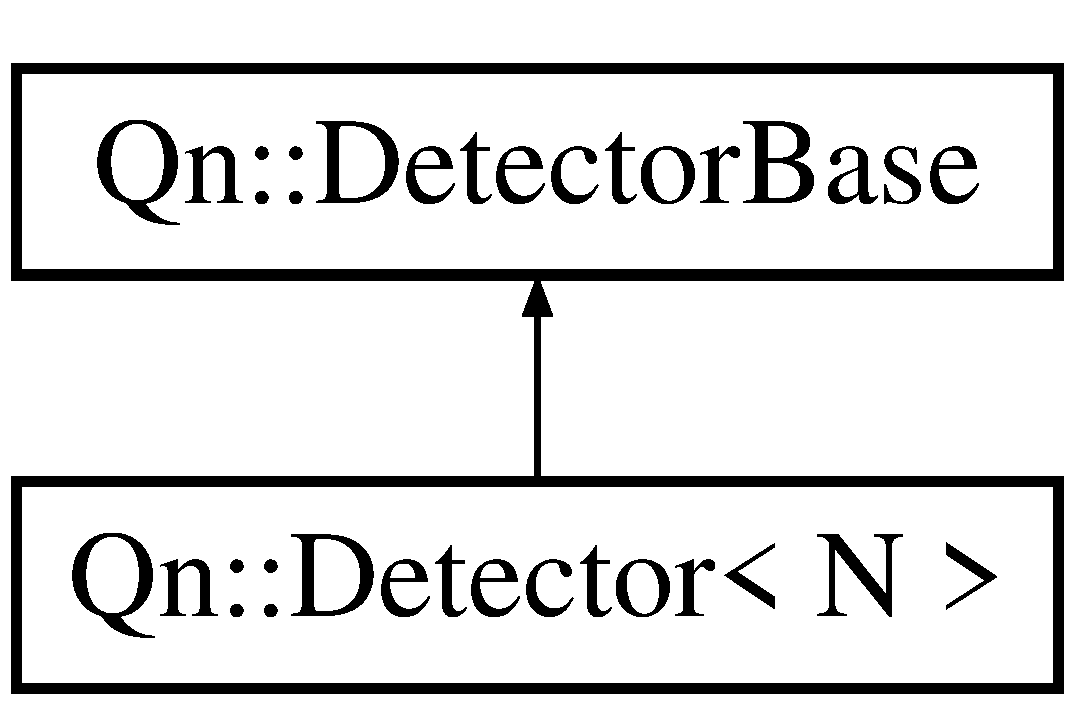
\includegraphics[height=2.000000cm]{classQn_1_1Detector}
\end{center}
\end{figure}
\subsection*{Public Member Functions}
\begin{DoxyCompactItemize}
\item 
\mbox{\Hypertarget{classQn_1_1Detector_ab47355f8ca0c2e5ed0efdca409db1e3f}\label{classQn_1_1Detector_ab47355f8ca0c2e5ed0efdca409db1e3f}} 
{\bfseries Detector} (std\+::string name, const \mbox{\hyperlink{namespaceQn_adba56b19bd9207127cdc7227d9e03a05}{Detector\+Type}} type, std\+::vector$<$ \mbox{\hyperlink{classQn_1_1Axis}{Qn\+::\+Axis}} $>$ axes, const \mbox{\hyperlink{classQn_1_1Variable}{Variable}} phi, const \mbox{\hyperlink{classQn_1_1Variable}{Variable}} weight, const std\+::vector$<$ \mbox{\hyperlink{classQn_1_1Variable}{Variable}} $>$ \&vars, int const(\&harmo)\mbox{[}N\mbox{]})
\item 
\mbox{\Hypertarget{classQn_1_1Detector_ab2e924f436158be1e6f7c1930117e82c}\label{classQn_1_1Detector_ab2e924f436158be1e6f7c1930117e82c}} 
void \mbox{\hyperlink{classQn_1_1Detector_ab2e924f436158be1e6f7c1930117e82c}{Clear\+Data}} () override
\begin{DoxyCompactList}\small\item\em Clears data before filling new event. \end{DoxyCompactList}\item 
\mbox{\hyperlink{classQn_1_1CorrectionDetector}{Correction\+Detector}} $\ast$ \mbox{\hyperlink{classQn_1_1Detector_a577f9c03f000ddab3fd0a2d69e02fc68}{Generate\+Detector}} (int globalid, int binid, \mbox{\hyperlink{classQn_1_1EventClassVariablesSet}{Event\+Class\+Variables\+Set}} $\ast$set) override
\item 
\mbox{\hyperlink{classQn_1_1DetectorConfiguration}{Detector\+Configuration}} $\ast$ \mbox{\hyperlink{classQn_1_1Detector_abf5ba68165d2e037b7c21911230ed288}{Create\+Detector\+Configuration}} (const std\+::string \&name, \mbox{\hyperlink{classQn_1_1EventClassVariablesSet}{Event\+Class\+Variables\+Set}} $\ast$set) override
\item 
std\+::unique\+\_\+ptr$<$ \mbox{\hyperlink{classQn_1_1DataContainer}{Data\+Container\+Data\+Vector}} $>$ \& \mbox{\hyperlink{classQn_1_1Detector_a3f08381bad2b1452a0209e420b99e989}{Get\+Data\+Container}} () override
\begin{DoxyCompactList}\small\item\em Get the datacontainer associated to the detector. \end{DoxyCompactList}\item 
std\+::unique\+\_\+ptr$<$ \mbox{\hyperlink{classQn_1_1DataContainer}{Data\+Container\+Q\+Vector}} $>$ \& \mbox{\hyperlink{classQn_1_1Detector_a9312033ff207a2caa762e895382f8456}{Get\+Qn\+Data\+Container}} () override
\begin{DoxyCompactList}\small\item\em Get the \mbox{\hyperlink{namespaceQn}{Qn}} vector data container associated to the detector. \end{DoxyCompactList}\item 
void \mbox{\hyperlink{classQn_1_1Detector_ac339acf64a05ab762a33137e2f00f84e}{Set\+Config}} (std\+::function$<$ void(\mbox{\hyperlink{classQn_1_1DetectorConfiguration}{Detector\+Configuration}} $\ast$config)$>$ conf) override
\begin{DoxyCompactList}\small\item\em Add the configuration function to the detector. \end{DoxyCompactList}\item 
void \mbox{\hyperlink{classQn_1_1Detector_a22b9795f3ae87d0b8ca483509907cbd1}{Add\+Cut}} (std\+::unique\+\_\+ptr$<$ \mbox{\hyperlink{structQn_1_1VariableCutBase}{Variable\+Cut\+Base}} $>$ cut) override
\begin{DoxyCompactList}\small\item\em Adds a cut to the detector. \end{DoxyCompactList}\item 
\mbox{\Hypertarget{classQn_1_1Detector_a977d0c05f4b3a3e7b117b28b3eca25b7}\label{classQn_1_1Detector_a977d0c05f4b3a3e7b117b28b3eca25b7}} 
void \mbox{\hyperlink{classQn_1_1Detector_a977d0c05f4b3a3e7b117b28b3eca25b7}{Fill\+Data}} () override
\begin{DoxyCompactList}\small\item\em Fills the data into the data vectors, histograms and cut reports after the cuts have been checked. \end{DoxyCompactList}\item 
void \mbox{\hyperlink{classQn_1_1Detector_a0dba51a9ca021046bdfa9c7af262b3f7}{Initialize\+Cut\+Reports}} () override
\item 
T\+List $\ast$ \mbox{\hyperlink{classQn_1_1Detector_a88a7d5c31a81624f9918c75220ffdd8a}{Get\+Report\+List}} () override
\begin{DoxyCompactList}\small\item\em Returns T\+List of QA and cut report histograms. \end{DoxyCompactList}\item 
void \mbox{\hyperlink{classQn_1_1Detector_a383267252d65877fa80fa7a0416e95bf}{Fill\+Report}} () override
\item 
void \mbox{\hyperlink{classQn_1_1Detector_a56d2dffc1f50b597edb95830f408b758}{Add\+Histogram}} (std\+::unique\+\_\+ptr$<$ \mbox{\hyperlink{structQn_1_1QAHistoBase}{Q\+A\+Histo\+Base}} $>$ histo) override
\begin{DoxyCompactList}\small\item\em Adds a QA histogram to the detector. \end{DoxyCompactList}\item 
void \mbox{\hyperlink{classQn_1_1Detector_aaaf2475cd8fa805dbca1fe22b72acdf5}{Set\+Up\+Correction\+Vector\+Ptrs}} (const \mbox{\hyperlink{classQn_1_1CorrectionCalculator}{Qn\+::\+Correction\+Calculator}} \&calc, std\+::string step) override
\begin{DoxyCompactList}\small\item\em Saves the pointers to the corrected Q vectors. \end{DoxyCompactList}\item 
\mbox{\Hypertarget{classQn_1_1Detector_a2d4f2a8e934ee6b89ac22f00adfca53d}\label{classQn_1_1Detector_a2d4f2a8e934ee6b89ac22f00adfca53d}} 
void \mbox{\hyperlink{classQn_1_1Detector_a2d4f2a8e934ee6b89ac22f00adfca53d}{Get\+Corrected\+Q\+Vectors}} () override
\begin{DoxyCompactList}\small\item\em Updates the Qvectors to the values retrieved from the correction calculator. This function is called every event before the output tree is filled. \end{DoxyCompactList}\end{DoxyCompactItemize}


\subsection{Detailed Description}
\subsubsection*{template$<$std\+::size\+\_\+t N$>$\newline
class Qn\+::\+Detector$<$ N $>$}

\mbox{\hyperlink{classQn_1_1Detector}{Detector}} class Template parameter automatically deduced. 
\begin{DoxyTemplParams}{Template Parameters}
{\em N} & number of harmonics activated. Harmonic max is 8. \\
\hline
\end{DoxyTemplParams}


\subsection{Member Function Documentation}
\mbox{\Hypertarget{classQn_1_1Detector_a22b9795f3ae87d0b8ca483509907cbd1}\label{classQn_1_1Detector_a22b9795f3ae87d0b8ca483509907cbd1}} 
\index{Qn\+::\+Detector@{Qn\+::\+Detector}!Add\+Cut@{Add\+Cut}}
\index{Add\+Cut@{Add\+Cut}!Qn\+::\+Detector@{Qn\+::\+Detector}}
\subsubsection{\texorpdfstring{Add\+Cut()}{AddCut()}}
{\footnotesize\ttfamily template$<$std\+::size\+\_\+t N$>$ \\
void \mbox{\hyperlink{classQn_1_1Detector}{Qn\+::\+Detector}}$<$ N $>$\+::Add\+Cut (\begin{DoxyParamCaption}\item[{std\+::unique\+\_\+ptr$<$ \mbox{\hyperlink{structQn_1_1VariableCutBase}{Variable\+Cut\+Base}} $>$}]{cut }\end{DoxyParamCaption})\hspace{0.3cm}{\ttfamily [inline]}, {\ttfamily [override]}, {\ttfamily [virtual]}}



Adds a cut to the detector. 


\begin{DoxyParams}{Parameters}
{\em cut} & unique pointer to the cut. It is moved into the function and cannot be reused! \\
\hline
\end{DoxyParams}


Implements \mbox{\hyperlink{classQn_1_1DetectorBase}{Qn\+::\+Detector\+Base}}.

\mbox{\Hypertarget{classQn_1_1Detector_a56d2dffc1f50b597edb95830f408b758}\label{classQn_1_1Detector_a56d2dffc1f50b597edb95830f408b758}} 
\index{Qn\+::\+Detector@{Qn\+::\+Detector}!Add\+Histogram@{Add\+Histogram}}
\index{Add\+Histogram@{Add\+Histogram}!Qn\+::\+Detector@{Qn\+::\+Detector}}
\subsubsection{\texorpdfstring{Add\+Histogram()}{AddHistogram()}}
{\footnotesize\ttfamily template$<$std\+::size\+\_\+t N$>$ \\
void \mbox{\hyperlink{classQn_1_1Detector}{Qn\+::\+Detector}}$<$ N $>$\+::Add\+Histogram (\begin{DoxyParamCaption}\item[{std\+::unique\+\_\+ptr$<$ \mbox{\hyperlink{structQn_1_1QAHistoBase}{Q\+A\+Histo\+Base}} $>$}]{histo }\end{DoxyParamCaption})\hspace{0.3cm}{\ttfamily [inline]}, {\ttfamily [override]}, {\ttfamily [virtual]}}



Adds a QA histogram to the detector. 


\begin{DoxyParams}{Parameters}
{\em histo} & pointer to the histogram. \\
\hline
\end{DoxyParams}


Implements \mbox{\hyperlink{classQn_1_1DetectorBase}{Qn\+::\+Detector\+Base}}.

\mbox{\Hypertarget{classQn_1_1Detector_abf5ba68165d2e037b7c21911230ed288}\label{classQn_1_1Detector_abf5ba68165d2e037b7c21911230ed288}} 
\index{Qn\+::\+Detector@{Qn\+::\+Detector}!Create\+Detector\+Configuration@{Create\+Detector\+Configuration}}
\index{Create\+Detector\+Configuration@{Create\+Detector\+Configuration}!Qn\+::\+Detector@{Qn\+::\+Detector}}
\subsubsection{\texorpdfstring{Create\+Detector\+Configuration()}{CreateDetectorConfiguration()}}
{\footnotesize\ttfamily template$<$std\+::size\+\_\+t N$>$ \\
\mbox{\hyperlink{classQn_1_1DetectorConfiguration}{Detector\+Configuration}}$\ast$ \mbox{\hyperlink{classQn_1_1Detector}{Qn\+::\+Detector}}$<$ N $>$\+::Create\+Detector\+Configuration (\begin{DoxyParamCaption}\item[{const std\+::string \&}]{name,  }\item[{\mbox{\hyperlink{classQn_1_1EventClassVariablesSet}{Event\+Class\+Variables\+Set}} $\ast$}]{set }\end{DoxyParamCaption})\hspace{0.3cm}{\ttfamily [inline]}, {\ttfamily [override]}, {\ttfamily [virtual]}}

Generate the detector configuration. 
\begin{DoxyParams}{Parameters}
{\em name} & Name of the detector \\
\hline
{\em set} & The set of event variables used for the configuration. \\
\hline
\end{DoxyParams}
\begin{DoxyReturn}{Returns}
The detector configuration. 
\end{DoxyReturn}


Implements \mbox{\hyperlink{classQn_1_1DetectorBase}{Qn\+::\+Detector\+Base}}.

\mbox{\Hypertarget{classQn_1_1Detector_a383267252d65877fa80fa7a0416e95bf}\label{classQn_1_1Detector_a383267252d65877fa80fa7a0416e95bf}} 
\index{Qn\+::\+Detector@{Qn\+::\+Detector}!Fill\+Report@{Fill\+Report}}
\index{Fill\+Report@{Fill\+Report}!Qn\+::\+Detector@{Qn\+::\+Detector}}
\subsubsection{\texorpdfstring{Fill\+Report()}{FillReport()}}
{\footnotesize\ttfamily template$<$std\+::size\+\_\+t N$>$ \\
void \mbox{\hyperlink{classQn_1_1Detector}{Qn\+::\+Detector}}$<$ N $>$\+::Fill\+Report (\begin{DoxyParamCaption}{ }\end{DoxyParamCaption})\hspace{0.3cm}{\ttfamily [inline]}, {\ttfamily [override]}, {\ttfamily [virtual]}}

Fill the cuts reports to the 

Implements \mbox{\hyperlink{classQn_1_1DetectorBase}{Qn\+::\+Detector\+Base}}.

\mbox{\Hypertarget{classQn_1_1Detector_a577f9c03f000ddab3fd0a2d69e02fc68}\label{classQn_1_1Detector_a577f9c03f000ddab3fd0a2d69e02fc68}} 
\index{Qn\+::\+Detector@{Qn\+::\+Detector}!Generate\+Detector@{Generate\+Detector}}
\index{Generate\+Detector@{Generate\+Detector}!Qn\+::\+Detector@{Qn\+::\+Detector}}
\subsubsection{\texorpdfstring{Generate\+Detector()}{GenerateDetector()}}
{\footnotesize\ttfamily template$<$std\+::size\+\_\+t N$>$ \\
\mbox{\hyperlink{classQn_1_1CorrectionDetector}{Correction\+Detector}}$\ast$ \mbox{\hyperlink{classQn_1_1Detector}{Qn\+::\+Detector}}$<$ N $>$\+::Generate\+Detector (\begin{DoxyParamCaption}\item[{int}]{globalid,  }\item[{int}]{binid,  }\item[{\mbox{\hyperlink{classQn_1_1EventClassVariablesSet}{Event\+Class\+Variables\+Set}} $\ast$}]{set }\end{DoxyParamCaption})\hspace{0.3cm}{\ttfamily [inline]}, {\ttfamily [override]}, {\ttfamily [virtual]}}

Generate the detector and configure the calibration procedure based on the preset configuration 
\begin{DoxyParams}{Parameters}
{\em globalid} & global ID used in the correction calculator. It is unique. \\
\hline
{\em binid} & local bin ID \\
\hline
{\em set} & the set of event variables used for correction. \\
\hline
\end{DoxyParams}
\begin{DoxyReturn}{Returns}
configured detector. 
\end{DoxyReturn}


Implements \mbox{\hyperlink{classQn_1_1DetectorBase}{Qn\+::\+Detector\+Base}}.

\mbox{\Hypertarget{classQn_1_1Detector_a3f08381bad2b1452a0209e420b99e989}\label{classQn_1_1Detector_a3f08381bad2b1452a0209e420b99e989}} 
\index{Qn\+::\+Detector@{Qn\+::\+Detector}!Get\+Data\+Container@{Get\+Data\+Container}}
\index{Get\+Data\+Container@{Get\+Data\+Container}!Qn\+::\+Detector@{Qn\+::\+Detector}}
\subsubsection{\texorpdfstring{Get\+Data\+Container()}{GetDataContainer()}}
{\footnotesize\ttfamily template$<$std\+::size\+\_\+t N$>$ \\
std\+::unique\+\_\+ptr$<$\mbox{\hyperlink{classQn_1_1DataContainer}{Data\+Container\+Data\+Vector}}$>$\& \mbox{\hyperlink{classQn_1_1Detector}{Qn\+::\+Detector}}$<$ N $>$\+::Get\+Data\+Container (\begin{DoxyParamCaption}{ }\end{DoxyParamCaption})\hspace{0.3cm}{\ttfamily [inline]}, {\ttfamily [override]}, {\ttfamily [virtual]}}



Get the datacontainer associated to the detector. 

\begin{DoxyReturn}{Returns}
A reference to the Datacontainer. 
\end{DoxyReturn}


Implements \mbox{\hyperlink{classQn_1_1DetectorBase}{Qn\+::\+Detector\+Base}}.

\mbox{\Hypertarget{classQn_1_1Detector_a9312033ff207a2caa762e895382f8456}\label{classQn_1_1Detector_a9312033ff207a2caa762e895382f8456}} 
\index{Qn\+::\+Detector@{Qn\+::\+Detector}!Get\+Qn\+Data\+Container@{Get\+Qn\+Data\+Container}}
\index{Get\+Qn\+Data\+Container@{Get\+Qn\+Data\+Container}!Qn\+::\+Detector@{Qn\+::\+Detector}}
\subsubsection{\texorpdfstring{Get\+Qn\+Data\+Container()}{GetQnDataContainer()}}
{\footnotesize\ttfamily template$<$std\+::size\+\_\+t N$>$ \\
std\+::unique\+\_\+ptr$<$\mbox{\hyperlink{classQn_1_1DataContainer}{Data\+Container\+Q\+Vector}}$>$\& \mbox{\hyperlink{classQn_1_1Detector}{Qn\+::\+Detector}}$<$ N $>$\+::Get\+Qn\+Data\+Container (\begin{DoxyParamCaption}{ }\end{DoxyParamCaption})\hspace{0.3cm}{\ttfamily [inline]}, {\ttfamily [override]}, {\ttfamily [virtual]}}



Get the \mbox{\hyperlink{namespaceQn}{Qn}} vector data container associated to the detector. 

\begin{DoxyReturn}{Returns}
A reference to the Datacontainer. 
\end{DoxyReturn}


Implements \mbox{\hyperlink{classQn_1_1DetectorBase}{Qn\+::\+Detector\+Base}}.

\mbox{\Hypertarget{classQn_1_1Detector_a88a7d5c31a81624f9918c75220ffdd8a}\label{classQn_1_1Detector_a88a7d5c31a81624f9918c75220ffdd8a}} 
\index{Qn\+::\+Detector@{Qn\+::\+Detector}!Get\+Report\+List@{Get\+Report\+List}}
\index{Get\+Report\+List@{Get\+Report\+List}!Qn\+::\+Detector@{Qn\+::\+Detector}}
\subsubsection{\texorpdfstring{Get\+Report\+List()}{GetReportList()}}
{\footnotesize\ttfamily template$<$std\+::size\+\_\+t N$>$ \\
T\+List$\ast$ \mbox{\hyperlink{classQn_1_1Detector}{Qn\+::\+Detector}}$<$ N $>$\+::Get\+Report\+List (\begin{DoxyParamCaption}{ }\end{DoxyParamCaption})\hspace{0.3cm}{\ttfamily [inline]}, {\ttfamily [override]}, {\ttfamily [virtual]}}



Returns T\+List of QA and cut report histograms. 

\begin{DoxyReturn}{Returns}
list of histograms. Lifetime managed by the user. 
\end{DoxyReturn}


Implements \mbox{\hyperlink{classQn_1_1DetectorBase}{Qn\+::\+Detector\+Base}}.

\mbox{\Hypertarget{classQn_1_1Detector_a0dba51a9ca021046bdfa9c7af262b3f7}\label{classQn_1_1Detector_a0dba51a9ca021046bdfa9c7af262b3f7}} 
\index{Qn\+::\+Detector@{Qn\+::\+Detector}!Initialize\+Cut\+Reports@{Initialize\+Cut\+Reports}}
\index{Initialize\+Cut\+Reports@{Initialize\+Cut\+Reports}!Qn\+::\+Detector@{Qn\+::\+Detector}}
\subsubsection{\texorpdfstring{Initialize\+Cut\+Reports()}{InitializeCutReports()}}
{\footnotesize\ttfamily template$<$std\+::size\+\_\+t N$>$ \\
void \mbox{\hyperlink{classQn_1_1Detector}{Qn\+::\+Detector}}$<$ N $>$\+::Initialize\+Cut\+Reports (\begin{DoxyParamCaption}{ }\end{DoxyParamCaption})\hspace{0.3cm}{\ttfamily [inline]}, {\ttfamily [override]}, {\ttfamily [virtual]}}

Initializes the histograms used for the cut report. 
\begin{DoxyParams}{Parameters}
{\em name} & name of the detector. \\
\hline
\end{DoxyParams}


Implements \mbox{\hyperlink{classQn_1_1DetectorBase}{Qn\+::\+Detector\+Base}}.

\mbox{\Hypertarget{classQn_1_1Detector_ac339acf64a05ab762a33137e2f00f84e}\label{classQn_1_1Detector_ac339acf64a05ab762a33137e2f00f84e}} 
\index{Qn\+::\+Detector@{Qn\+::\+Detector}!Set\+Config@{Set\+Config}}
\index{Set\+Config@{Set\+Config}!Qn\+::\+Detector@{Qn\+::\+Detector}}
\subsubsection{\texorpdfstring{Set\+Config()}{SetConfig()}}
{\footnotesize\ttfamily template$<$std\+::size\+\_\+t N$>$ \\
void \mbox{\hyperlink{classQn_1_1Detector}{Qn\+::\+Detector}}$<$ N $>$\+::Set\+Config (\begin{DoxyParamCaption}\item[{std\+::function$<$ void(\mbox{\hyperlink{classQn_1_1DetectorConfiguration}{Detector\+Configuration}} $\ast$config)$>$}]{conf }\end{DoxyParamCaption})\hspace{0.3cm}{\ttfamily [inline]}, {\ttfamily [override]}, {\ttfamily [virtual]}}



Add the configuration function to the detector. 


\begin{DoxyParams}{Parameters}
{\em conf} & function which configures the detector. needs to have the specified form. \\
\hline
\end{DoxyParams}


Implements \mbox{\hyperlink{classQn_1_1DetectorBase}{Qn\+::\+Detector\+Base}}.

\mbox{\Hypertarget{classQn_1_1Detector_aaaf2475cd8fa805dbca1fe22b72acdf5}\label{classQn_1_1Detector_aaaf2475cd8fa805dbca1fe22b72acdf5}} 
\index{Qn\+::\+Detector@{Qn\+::\+Detector}!Set\+Up\+Correction\+Vector\+Ptrs@{Set\+Up\+Correction\+Vector\+Ptrs}}
\index{Set\+Up\+Correction\+Vector\+Ptrs@{Set\+Up\+Correction\+Vector\+Ptrs}!Qn\+::\+Detector@{Qn\+::\+Detector}}
\subsubsection{\texorpdfstring{Set\+Up\+Correction\+Vector\+Ptrs()}{SetUpCorrectionVectorPtrs()}}
{\footnotesize\ttfamily template$<$std\+::size\+\_\+t N$>$ \\
void \mbox{\hyperlink{classQn_1_1Detector}{Qn\+::\+Detector}}$<$ N $>$\+::Set\+Up\+Correction\+Vector\+Ptrs (\begin{DoxyParamCaption}\item[{const \mbox{\hyperlink{classQn_1_1CorrectionCalculator}{Qn\+::\+Correction\+Calculator}} \&}]{calc,  }\item[{std\+::string}]{step }\end{DoxyParamCaption})\hspace{0.3cm}{\ttfamily [inline]}, {\ttfamily [override]}, {\ttfamily [virtual]}}



Saves the pointers to the corrected Q vectors. 


\begin{DoxyParams}{Parameters}
{\em calc} & reference to the correction calculator. \\
\hline
{\em step} & specification which correction step is supposed to be retrieved. \\
\hline
\end{DoxyParams}


Implements \mbox{\hyperlink{classQn_1_1DetectorBase}{Qn\+::\+Detector\+Base}}.



The documentation for this class was generated from the following file\+:\begin{DoxyCompactItemize}
\item 
D\+T\+\_\+\+Flow/\+Correction/include/Detector.\+h\end{DoxyCompactItemize}

\hypertarget{classQn_1_1DetectorBase}{}\section{Qn\+:\+:Detector\+Base Class Reference}
\label{classQn_1_1DetectorBase}\index{Qn\+::\+Detector\+Base@{Qn\+::\+Detector\+Base}}
Inheritance diagram for Qn\+:\+:Detector\+Base\+:\begin{figure}[H]
\begin{center}
\leavevmode
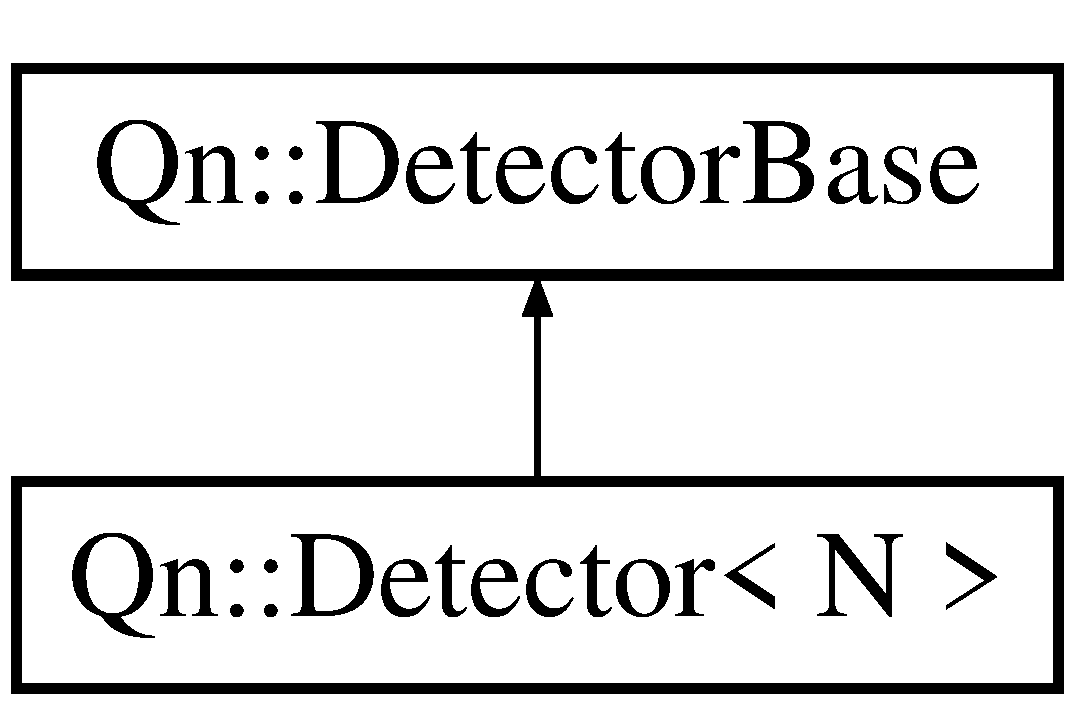
\includegraphics[height=2.000000cm]{classQn_1_1DetectorBase}
\end{center}
\end{figure}
\subsection*{Public Member Functions}
\begin{DoxyCompactItemize}
\item 
\mbox{\Hypertarget{classQn_1_1DetectorBase_a5123507d64cd89af08f8f5ed56dffc22}\label{classQn_1_1DetectorBase_a5123507d64cd89af08f8f5ed56dffc22}} 
virtual std\+::unique\+\_\+ptr$<$ \mbox{\hyperlink{classQn_1_1DataContainer}{Data\+Container\+Data\+Vector}} $>$ \& {\bfseries Get\+Data\+Container} ()=0
\item 
\mbox{\Hypertarget{classQn_1_1DetectorBase_a92928192623525ba5b74b1082c9b482c}\label{classQn_1_1DetectorBase_a92928192623525ba5b74b1082c9b482c}} 
virtual std\+::unique\+\_\+ptr$<$ \mbox{\hyperlink{classQn_1_1DataContainer}{Data\+Container\+Q\+Vector}} $>$ \& {\bfseries Get\+Qn\+Data\+Container} ()=0
\item 
\mbox{\Hypertarget{classQn_1_1DetectorBase_acfc970cde94b5d09a3d1316fb3d6e36f}\label{classQn_1_1DetectorBase_acfc970cde94b5d09a3d1316fb3d6e36f}} 
virtual \mbox{\hyperlink{classQn_1_1CorrectionDetector}{Correction\+Detector}} $\ast$ {\bfseries Generate\+Detector} (int globalid, int binid, \mbox{\hyperlink{classQn_1_1EventClassVariablesSet}{Event\+Class\+Variables\+Set}} $\ast$set)=0
\item 
\mbox{\Hypertarget{classQn_1_1DetectorBase_a720efe2f7086b4c7f68edf95d214a93a}\label{classQn_1_1DetectorBase_a720efe2f7086b4c7f68edf95d214a93a}} 
virtual \mbox{\hyperlink{classQn_1_1DetectorConfiguration}{Detector\+Configuration}} $\ast$ {\bfseries Create\+Detector\+Configuration} (const std\+::string \&name, \mbox{\hyperlink{classQn_1_1EventClassVariablesSet}{Event\+Class\+Variables\+Set}} $\ast$set)=0
\item 
\mbox{\Hypertarget{classQn_1_1DetectorBase_a83e9646091bccacffa297f0b23f5cb09}\label{classQn_1_1DetectorBase_a83e9646091bccacffa297f0b23f5cb09}} 
virtual void {\bfseries Set\+Config} (std\+::function$<$ void(\mbox{\hyperlink{classQn_1_1DetectorConfiguration}{Detector\+Configuration}} $\ast$config)$>$ conf)=0
\item 
\mbox{\Hypertarget{classQn_1_1DetectorBase_a95630775362a14958ef270dc115c5679}\label{classQn_1_1DetectorBase_a95630775362a14958ef270dc115c5679}} 
virtual void {\bfseries Add\+Cut} (std\+::unique\+\_\+ptr$<$ \mbox{\hyperlink{structQn_1_1VariableCutBase}{Variable\+Cut\+Base}} $>$ cut)=0
\item 
\mbox{\Hypertarget{classQn_1_1DetectorBase_a1d85af0a10390f65223cae91b7ef2883}\label{classQn_1_1DetectorBase_a1d85af0a10390f65223cae91b7ef2883}} 
virtual void {\bfseries Add\+Histogram} (std\+::unique\+\_\+ptr$<$ \mbox{\hyperlink{structQn_1_1QAHistoBase}{Q\+A\+Histo\+Base}} $>$ base)=0
\item 
\mbox{\Hypertarget{classQn_1_1DetectorBase_a777b04c1abfff3d28caecf0cb86fb3e7}\label{classQn_1_1DetectorBase_a777b04c1abfff3d28caecf0cb86fb3e7}} 
virtual void {\bfseries Initialize\+Cut\+Reports} ()=0
\item 
\mbox{\Hypertarget{classQn_1_1DetectorBase_aad5889793f34ee5c80a4fc7471cd8b96}\label{classQn_1_1DetectorBase_aad5889793f34ee5c80a4fc7471cd8b96}} 
virtual void {\bfseries Fill\+Report} ()=0
\item 
\mbox{\Hypertarget{classQn_1_1DetectorBase_ad18b602694b1cd392c63d2f456e02377}\label{classQn_1_1DetectorBase_ad18b602694b1cd392c63d2f456e02377}} 
virtual void {\bfseries Fill\+Data} ()=0
\item 
\mbox{\Hypertarget{classQn_1_1DetectorBase_a8833f5bd09a569bf3795058c3e4da528}\label{classQn_1_1DetectorBase_a8833f5bd09a569bf3795058c3e4da528}} 
virtual void {\bfseries Clear\+Data} ()=0
\item 
\mbox{\Hypertarget{classQn_1_1DetectorBase_a1399c579dcc65d191bd92a3edeb9d6fe}\label{classQn_1_1DetectorBase_a1399c579dcc65d191bd92a3edeb9d6fe}} 
virtual T\+List $\ast$ {\bfseries Get\+Report\+List} ()=0
\item 
\mbox{\Hypertarget{classQn_1_1DetectorBase_aa9d6c4d75884271c2af8fff506f84207}\label{classQn_1_1DetectorBase_aa9d6c4d75884271c2af8fff506f84207}} 
virtual void {\bfseries Set\+Up\+Correction\+Vector\+Ptrs} (const \mbox{\hyperlink{classQn_1_1CorrectionCalculator}{Qn\+::\+Correction\+Calculator}} \&calc, std\+::string step)=0
\item 
\mbox{\Hypertarget{classQn_1_1DetectorBase_aedb870c235ad5f03630b6670ebd2b151}\label{classQn_1_1DetectorBase_aedb870c235ad5f03630b6670ebd2b151}} 
virtual void {\bfseries Get\+Corrected\+Q\+Vectors} ()=0
\end{DoxyCompactItemize}


The documentation for this class was generated from the following file\+:\begin{DoxyCompactItemize}
\item 
D\+T\+\_\+\+Flow/\+Correction/include/Detector.\+h\end{DoxyCompactItemize}

\hypertarget{classQn_1_1DetectorConfiguration}{}\section{Qn\+:\+:Detector\+Configuration Class Reference}
\label{classQn_1_1DetectorConfiguration}\index{Qn\+::\+Detector\+Configuration@{Qn\+::\+Detector\+Configuration}}
Inheritance diagram for Qn\+:\+:Detector\+Configuration\+:\begin{figure}[H]
\begin{center}
\leavevmode
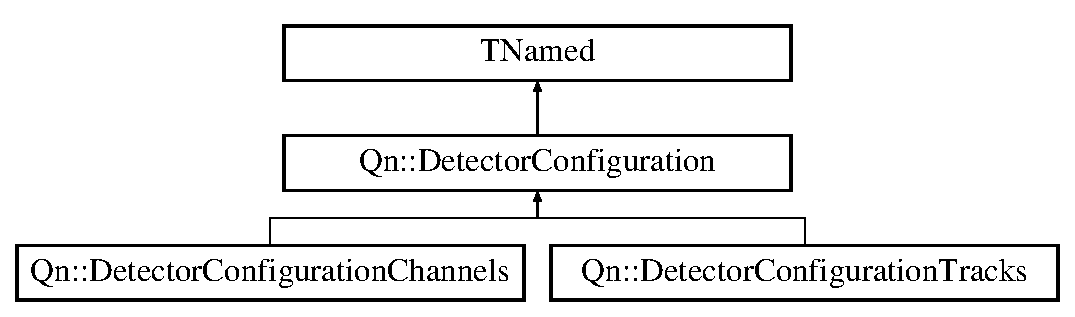
\includegraphics[height=3.000000cm]{classQn_1_1DetectorConfiguration}
\end{center}
\end{figure}
\subsection*{Public Member Functions}
\begin{DoxyCompactItemize}
\item 
\mbox{\Hypertarget{classQn_1_1DetectorConfiguration_aa4d47ee6636f8a0a16cf765ea5652717}\label{classQn_1_1DetectorConfiguration_aa4d47ee6636f8a0a16cf765ea5652717}} 
\mbox{\hyperlink{classQn_1_1DetectorConfiguration_aa4d47ee6636f8a0a16cf765ea5652717}{Detector\+Configuration}} ()
\begin{DoxyCompactList}\small\item\em Default constructor. \end{DoxyCompactList}\item 
\mbox{\hyperlink{classQn_1_1DetectorConfiguration_ace49da97614ea3268a6483a5f0b4a1c5}{Detector\+Configuration}} (const char $\ast$name, \mbox{\hyperlink{classQn_1_1EventClassVariablesSet}{Event\+Class\+Variables\+Set}} $\ast$event\+Classes\+Variables, Int\+\_\+t n\+No\+Of\+Harmonics, Int\+\_\+t $\ast$harmonic\+Map=N\+U\+LL)
\item 
virtual \mbox{\hyperlink{classQn_1_1DetectorConfiguration_a19aab70fc76c6adf6af8586e74c85048}{$\sim$\+Detector\+Configuration}} ()
\item 
void \mbox{\hyperlink{classQn_1_1DetectorConfiguration_a740b364553bfc9306e6b486093dcf227}{Set\+Cuts}} (\mbox{\hyperlink{classQn_1_1CutsSet}{Cuts\+Set}} $\ast$cuts)
\item 
void \mbox{\hyperlink{classQn_1_1DetectorConfiguration_a018d9391fa2fbe6fe3c3d1dd5c3389d7}{Set\+Normalization}} (\mbox{\hyperlink{classQn_1_1CorrectionQnVector_a2998fe4babb716c57848c8c73b24a398}{Correction\+Qn\+Vector\+::\+Normalization}} method)
\item 
\mbox{\Hypertarget{classQn_1_1DetectorConfiguration_ae260877a44955bddcc5ae238f07a33d0}\label{classQn_1_1DetectorConfiguration_ae260877a44955bddcc5ae238f07a33d0}} 
\mbox{\hyperlink{classQn_1_1CorrectionQnVector_a2998fe4babb716c57848c8c73b24a398}{Correction\+Qn\+Vector\+::\+Normalization}} \mbox{\hyperlink{classQn_1_1DetectorConfiguration_ae260877a44955bddcc5ae238f07a33d0}{Get\+Q\+Vector\+Normalization\+Method}} () const
\begin{DoxyCompactList}\small\item\em Get the normalization method for Q vectors. \end{DoxyCompactList}\item 
void \mbox{\hyperlink{classQn_1_1DetectorConfiguration_a100aab7b32a43830dc1dc9eac5b2a158}{Set\+Detector\+Owner}} (\mbox{\hyperlink{classQn_1_1CorrectionDetector}{Correction\+Detector}} $\ast$detector)
\item 
\mbox{\hyperlink{classQn_1_1CorrectionDetector}{Correction\+Detector}} $\ast$ \mbox{\hyperlink{classQn_1_1DetectorConfiguration_a2a34cbc491d83fd5073bc4e9bb0d4943}{Get\+Detector}} ()
\item 
virtual void \mbox{\hyperlink{classQn_1_1DetectorConfiguration_a512c77d73e0e6453607f7ae7e2e8f72b}{Attach\+Corrections\+Manager}} (\mbox{\hyperlink{classQn_1_1CorrectionCalculator}{Correction\+Calculator}} $\ast$manager)=0
\item 
T\+Clones\+Array $\ast$ \mbox{\hyperlink{classQn_1_1DetectorConfiguration_a80b18020e8636295cdea1dd2c11449d3}{Get\+Input\+Data\+Bank}} ()
\item 
\mbox{\hyperlink{classQn_1_1EventClassVariablesSet}{Event\+Class\+Variables\+Set}} \& \mbox{\hyperlink{classQn_1_1DetectorConfiguration_a77df91021253bf6e5320bfe52b7147d7}{Get\+Event\+Class\+Variables\+Set}} ()
\item 
\mbox{\hyperlink{classQn_1_1CorrectionQnVector}{Correction\+Qn\+Vector}} $\ast$ \mbox{\hyperlink{classQn_1_1DetectorConfiguration_ae467babb14df7f6b264eb379dceff2dd}{Get\+Current\+Qn\+Vector}} ()
\item 
const \mbox{\hyperlink{classQn_1_1CorrectionQnVector}{Correction\+Qn\+Vector}} $\ast$ \mbox{\hyperlink{classQn_1_1DetectorConfiguration_aac09cc211d9fc911b61dbe14fdc4f5f3}{Get\+Previous\+Corrected\+Qn\+Vector}} (\mbox{\hyperlink{classQn_1_1CorrectionOnQvector}{Correction\+On\+Qvector}} $\ast$correction\+On\+Qn) const
\item 
Bool\+\_\+t \mbox{\hyperlink{classQn_1_1DetectorConfiguration_a25fce09641fb89b686154a6d6bad823a}{Is\+Correction\+Step\+Being\+Applied}} (const char $\ast$step) const
\item 
\mbox{\hyperlink{classQn_1_1CorrectionQnVector}{Correction\+Qn\+Vector}} $\ast$ \mbox{\hyperlink{classQn_1_1DetectorConfiguration_a8f2e955fc14f8db870a89fc4ab1dc36b}{Get\+Current\+Q2n\+Vector}} ()
\item 
\mbox{\hyperlink{classQn_1_1CorrectionQnVector}{Correction\+Qn\+Vector}} $\ast$ \mbox{\hyperlink{classQn_1_1DetectorConfiguration_a3d5ca70800045c579f4bda073a382f68}{Get\+Plain\+Qn\+Vector}} ()
\item 
\mbox{\hyperlink{classQn_1_1CorrectionQnVector}{Correction\+Qn\+Vector}} $\ast$ \mbox{\hyperlink{classQn_1_1DetectorConfiguration_a25396b7997264f317e5c4ee7d3dcaeac}{Get\+Plain\+Q2n\+Vector}} ()
\item 
void \mbox{\hyperlink{classQn_1_1DetectorConfiguration_a6e7228b694e8a1a15290c711f870a527}{Update\+Current\+Qn\+Vector}} (\mbox{\hyperlink{classQn_1_1CorrectionQnVector}{Correction\+Qn\+Vector}} $\ast$new\+Qn\+Vector, Bool\+\_\+t changename=k\+T\+R\+UE)
\item 
void \mbox{\hyperlink{classQn_1_1DetectorConfiguration_abeabec819fe0cab801d7afbe185abe40}{Update\+Current\+Q2n\+Vector}} (\mbox{\hyperlink{classQn_1_1CorrectionQnVector}{Correction\+Qn\+Vector}} $\ast$new\+Q2n\+Vector, Bool\+\_\+t changename=k\+T\+R\+UE)
\item 
Int\+\_\+t \mbox{\hyperlink{classQn_1_1DetectorConfiguration_a88f8b14da5e8faa8fd2548c6ab06f68a}{Get\+No\+Of\+Harmonics}} () const
\item 
void \mbox{\hyperlink{classQn_1_1DetectorConfiguration_a3e8079b295c46564e525072dab4ae055}{Get\+Harmonic\+Map}} (Int\+\_\+t $\ast$store) const
\item 
\mbox{\hyperlink{classQn_1_1CorrectionCalculator}{Correction\+Calculator}} $\ast$ \mbox{\hyperlink{classQn_1_1DetectorConfiguration_a20a27b09e0d2f3209b8de97906c52711}{Get\+Corrections\+Manager}} () const
\item 
virtual Bool\+\_\+t \mbox{\hyperlink{classQn_1_1DetectorConfiguration_acdb57db96ed24524b5a3a28821727a3d}{Get\+Is\+Tracking\+Detector}} () const =0
\item 
virtual void \mbox{\hyperlink{classQn_1_1DetectorConfiguration_a664f65925f22f8f02c1a216f77b533ce}{Create\+Support\+Data\+Structures}} ()=0
\item 
virtual Bool\+\_\+t \mbox{\hyperlink{classQn_1_1DetectorConfiguration_a8e5e2eef94bca58a3dcf34fe5fbd1429}{Create\+Support\+Histograms}} (T\+List $\ast$list)=0
\item 
virtual Bool\+\_\+t \mbox{\hyperlink{classQn_1_1DetectorConfiguration_a9f527d4c584e6bd79b6b8eb0b7f5413a}{Create\+Q\+A\+Histograms}} (T\+List $\ast$list)=0
\item 
virtual Bool\+\_\+t \mbox{\hyperlink{classQn_1_1DetectorConfiguration_ade61875d8e7a05dd413c94d6887ae4ac}{Create\+Nve\+Q\+A\+Histograms}} (T\+List $\ast$list)=0
\item 
virtual Bool\+\_\+t \mbox{\hyperlink{classQn_1_1DetectorConfiguration_a4ae0eb587070e68a11fbb438d96fca15}{Attach\+Correction\+Inputs}} (T\+List $\ast$list)=0
\item 
virtual void \mbox{\hyperlink{classQn_1_1DetectorConfiguration_ab6766905dffe5811aefa59dd1e1117d8}{After\+Inputs\+Attach\+Actions}} ()=0
\item 
virtual Bool\+\_\+t \mbox{\hyperlink{classQn_1_1DetectorConfiguration_aad0610bd5d168c29a32025ddf641e3fc}{Process\+Corrections}} (const double $\ast$variable\+Container)=0
\item 
virtual Bool\+\_\+t \mbox{\hyperlink{classQn_1_1DetectorConfiguration_ac78ed44b460217fda7d094cc102504c4}{Process\+Data\+Collection}} (const double $\ast$variable\+Container)=0
\item 
virtual void \mbox{\hyperlink{classQn_1_1DetectorConfiguration_a5bb71f7e186c058cad8c6bba4f2596cd}{Activate\+Harmonic}} (Int\+\_\+t harmonic)
\item 
virtual void \mbox{\hyperlink{classQn_1_1DetectorConfiguration_a7c6c8b72521714d859c0c718cba9db5b}{Add\+Correction\+On\+Qn\+Vector}} (\mbox{\hyperlink{classQn_1_1CorrectionOnQvector}{Correction\+On\+Qvector}} $\ast$correction\+On\+Qn)
\item 
virtual void \mbox{\hyperlink{classQn_1_1DetectorConfiguration_ab65571f46d348c2b07d3b03fc1e6cf11}{Add\+Correction\+On\+Input\+Data}} (\mbox{\hyperlink{classQn_1_1CorrectionOnInputData}{Correction\+On\+Input\+Data}} $\ast$correction\+On\+Input\+Data)
\item 
virtual void \mbox{\hyperlink{classQn_1_1DetectorConfiguration_a7aaf10f6e30151dd142d59d5dff72e2d}{Build\+Qn\+Vector}} ()=0
\item 
virtual void \mbox{\hyperlink{classQn_1_1DetectorConfiguration_a4298530954cc8dabbd41b1fd83d6310f}{Include\+Qn\+Vectors}} (T\+List $\ast$list)=0
\item 
virtual void \mbox{\hyperlink{classQn_1_1DetectorConfiguration_a76e173f938b886b5575597d9464698b4}{Fill\+Overall\+Input\+Correction\+Step\+List}} (T\+List $\ast$list) const =0
\item 
virtual void \mbox{\hyperlink{classQn_1_1DetectorConfiguration_ad71d83a2b0a5cee45bde15e936843e49}{Fill\+Overall\+Qn\+Vector\+Correction\+Step\+List}} (T\+List $\ast$list) const =0
\item 
virtual void \mbox{\hyperlink{classQn_1_1DetectorConfiguration_ad33e54cbf374fa37d8edf9915719982f}{Report\+On\+Corrections}} (T\+List $\ast$steps, T\+List $\ast$calib, T\+List $\ast$apply) const =0
\item 
virtual Bool\+\_\+t \mbox{\hyperlink{classQn_1_1DetectorConfiguration_ab406e0d2a85e7f5a7c74d0bd0252375d}{Add\+Data\+Vector}} (const double $\ast$variable\+Container, Double\+\_\+t phi, Double\+\_\+t weight, Int\+\_\+t channel\+Id)=0
\item 
\mbox{\Hypertarget{classQn_1_1DetectorConfiguration_a3d29b2d5f068113b03a8d620044028dc}\label{classQn_1_1DetectorConfiguration_a3d29b2d5f068113b03a8d620044028dc}} 
virtual Bool\+\_\+t {\bfseries Is\+Selected} (const double $\ast$variable\+Container)=0
\item 
\mbox{\Hypertarget{classQn_1_1DetectorConfiguration_a41c2a9d6f9d74fc00e6bd9c9036aab9c}\label{classQn_1_1DetectorConfiguration_a41c2a9d6f9d74fc00e6bd9c9036aab9c}} 
virtual Bool\+\_\+t {\bfseries Is\+Selected} (const double $\ast$variable\+Container, Int\+\_\+t n\+Channel)=0
\item 
virtual void \mbox{\hyperlink{classQn_1_1DetectorConfiguration_a94c21b39a4a3680675319aacf4a517f4}{Clear\+Configuration}} ()=0
\item 
\mbox{\Hypertarget{classQn_1_1DetectorConfiguration_aad59ea03836959a6c8287bc6112f1443}\label{classQn_1_1DetectorConfiguration_aad59ea03836959a6c8287bc6112f1443}} 
virtual void {\bfseries Set\+Channels\+Scheme} (Bool\+\_\+t $\ast$b\+Used\+Channel, Int\+\_\+t $\ast$n\+Channel\+Group=nullptr, Float\+\_\+t $\ast$hard\+Coded\+Group\+Weights=nullptr)
\end{DoxyCompactItemize}
\subsection*{Protected Attributes}
\begin{DoxyCompactItemize}
\item 
\mbox{\Hypertarget{classQn_1_1DetectorConfiguration_a247561be3576d9e7ed644da70dc4f4b6}\label{classQn_1_1DetectorConfiguration_a247561be3576d9e7ed644da70dc4f4b6}} 
\mbox{\hyperlink{classQn_1_1CorrectionCalculator}{Correction\+Calculator}} $\ast$ \mbox{\hyperlink{classQn_1_1DetectorConfiguration_a247561be3576d9e7ed644da70dc4f4b6}{f\+Corrections\+Manager}}
\begin{DoxyCompactList}\small\item\em set of cuts that define the detector configuration \end{DoxyCompactList}\item 
\mbox{\Hypertarget{classQn_1_1DetectorConfiguration_ab1deed09e33f525995c05e44df64efe2}\label{classQn_1_1DetectorConfiguration_ab1deed09e33f525995c05e44df64efe2}} 
\mbox{\hyperlink{classQn_1_1CutsSet}{Cuts\+Set}} $\ast$ \mbox{\hyperlink{classQn_1_1DetectorConfiguration_ab1deed09e33f525995c05e44df64efe2}{f\+Cuts}}
\begin{DoxyCompactList}\small\item\em the framework manager pointer \end{DoxyCompactList}\item 
\mbox{\Hypertarget{classQn_1_1DetectorConfiguration_a2e9cf77ef7a6c224efe1a6ac54a588fe}\label{classQn_1_1DetectorConfiguration_a2e9cf77ef7a6c224efe1a6ac54a588fe}} 
T\+Clones\+Array $\ast$ \mbox{\hyperlink{classQn_1_1DetectorConfiguration_a2e9cf77ef7a6c224efe1a6ac54a588fe}{f\+Data\+Vector\+Bank}}
\begin{DoxyCompactList}\small\item\em ! input data for the current process / event \end{DoxyCompactList}\item 
\mbox{\Hypertarget{classQn_1_1DetectorConfiguration_a208a2442ee47a87720a41d32c80b1cb9}\label{classQn_1_1DetectorConfiguration_a208a2442ee47a87720a41d32c80b1cb9}} 
\mbox{\hyperlink{classQn_1_1CorrectionQnVector}{Correction\+Qn\+Vector}} \mbox{\hyperlink{classQn_1_1DetectorConfiguration_a208a2442ee47a87720a41d32c80b1cb9}{f\+Plain\+Qn\+Vector}}
\begin{DoxyCompactList}\small\item\em \mbox{\hyperlink{namespaceQn}{Qn}} vector from the post processed input data. \end{DoxyCompactList}\item 
\mbox{\Hypertarget{classQn_1_1DetectorConfiguration_ad375b588b3c1dbd119cbb4d93550d80c}\label{classQn_1_1DetectorConfiguration_ad375b588b3c1dbd119cbb4d93550d80c}} 
\mbox{\hyperlink{classQn_1_1CorrectionQnVector}{Correction\+Qn\+Vector}} \mbox{\hyperlink{classQn_1_1DetectorConfiguration_ad375b588b3c1dbd119cbb4d93550d80c}{f\+Plain\+Q2n\+Vector}}
\begin{DoxyCompactList}\small\item\em Q2n vector from the post processed input data. \end{DoxyCompactList}\item 
\mbox{\Hypertarget{classQn_1_1DetectorConfiguration_a39e1748fbe04d9bf144c69e17c0990ff}\label{classQn_1_1DetectorConfiguration_a39e1748fbe04d9bf144c69e17c0990ff}} 
\mbox{\hyperlink{classQn_1_1CorrectionQnVector}{Correction\+Qn\+Vector}} \mbox{\hyperlink{classQn_1_1DetectorConfiguration_a39e1748fbe04d9bf144c69e17c0990ff}{f\+Corrected\+Qn\+Vector}}
\begin{DoxyCompactList}\small\item\em \mbox{\hyperlink{namespaceQn}{Qn}} vector after subsequent correction steps. \end{DoxyCompactList}\item 
\mbox{\Hypertarget{classQn_1_1DetectorConfiguration_adee6ec50732e1966ab3294cd84f1bddb}\label{classQn_1_1DetectorConfiguration_adee6ec50732e1966ab3294cd84f1bddb}} 
\mbox{\hyperlink{classQn_1_1CorrectionQnVector}{Correction\+Qn\+Vector}} \mbox{\hyperlink{classQn_1_1DetectorConfiguration_adee6ec50732e1966ab3294cd84f1bddb}{f\+Corrected\+Q2n\+Vector}}
\begin{DoxyCompactList}\small\item\em Q2n vector after subsequent correction steps. \end{DoxyCompactList}\item 
\mbox{\Hypertarget{classQn_1_1DetectorConfiguration_a1a7961c7f7d2253986b7aa3aacdeb5fe}\label{classQn_1_1DetectorConfiguration_a1a7961c7f7d2253986b7aa3aacdeb5fe}} 
\mbox{\hyperlink{classQn_1_1CorrectionQnVectorBuild}{Correction\+Qn\+Vector\+Build}} \mbox{\hyperlink{classQn_1_1DetectorConfiguration_a1a7961c7f7d2253986b7aa3aacdeb5fe}{f\+Temp\+Qn\+Vector}}
\begin{DoxyCompactList}\small\item\em temporary \mbox{\hyperlink{namespaceQn}{Qn}} vector for efficient Q vector building \end{DoxyCompactList}\item 
\mbox{\Hypertarget{classQn_1_1DetectorConfiguration_a584998a6dccd234be7aa2bc881412dc5}\label{classQn_1_1DetectorConfiguration_a584998a6dccd234be7aa2bc881412dc5}} 
\mbox{\hyperlink{classQn_1_1CorrectionQnVectorBuild}{Correction\+Qn\+Vector\+Build}} \mbox{\hyperlink{classQn_1_1DetectorConfiguration_a584998a6dccd234be7aa2bc881412dc5}{f\+Temp\+Q2n\+Vector}}
\begin{DoxyCompactList}\small\item\em temporary \mbox{\hyperlink{namespaceQn}{Qn}} vector for efficient Q vector building \end{DoxyCompactList}\item 
\mbox{\Hypertarget{classQn_1_1DetectorConfiguration_a60cd5bf388c9fb4be34e779bfc56c0f4}\label{classQn_1_1DetectorConfiguration_a60cd5bf388c9fb4be34e779bfc56c0f4}} 
\mbox{\hyperlink{classQn_1_1CorrectionQnVector_a2998fe4babb716c57848c8c73b24a398}{Correction\+Qn\+Vector\+::\+Normalization}} \mbox{\hyperlink{classQn_1_1DetectorConfiguration_a60cd5bf388c9fb4be34e779bfc56c0f4}{f\+Qn\+Normalization\+Method}}
\begin{DoxyCompactList}\small\item\em the method for Q vector normalization \end{DoxyCompactList}\item 
\mbox{\hyperlink{classQn_1_1CorrectionsSetOnQvector}{Corrections\+Set\+On\+Qvector}} \mbox{\hyperlink{classQn_1_1DetectorConfiguration_aa25d2e08bd0e206475972657447ecf33}{f\+Qn\+Vector\+Corrections}}
\item 
\mbox{\Hypertarget{classQn_1_1DetectorConfiguration_a50e96e366c1207556587c75f47b0db27}\label{classQn_1_1DetectorConfiguration_a50e96e366c1207556587c75f47b0db27}} 
\mbox{\hyperlink{classQn_1_1EventClassVariablesSet}{Event\+Class\+Variables\+Set}} $\ast$ \mbox{\hyperlink{classQn_1_1DetectorConfiguration_a50e96e366c1207556587c75f47b0db27}{f\+Event\+Class\+Variables}}
\begin{DoxyCompactList}\small\item\em set of variables that define event classes \end{DoxyCompactList}\end{DoxyCompactItemize}
\subsection*{Static Protected Attributes}
\begin{DoxyCompactItemize}
\item 
static const char $\ast$ \mbox{\hyperlink{classQn_1_1DetectorConfiguration_a72caf89bf39a06cb23346bec00948c08}{sz\+Plain\+Qn\+Vector\+Name}} = \char`\"{}plain\char`\"{}
\end{DoxyCompactItemize}
\subsection*{Friends}
\begin{DoxyCompactItemize}
\item 
\mbox{\Hypertarget{classQn_1_1DetectorConfiguration_afbb351f0a159c2e61159977b03f4b3c1}\label{classQn_1_1DetectorConfiguration_afbb351f0a159c2e61159977b03f4b3c1}} 
class {\bfseries Correction\+Step\+Base}
\item 
\mbox{\Hypertarget{classQn_1_1DetectorConfiguration_aaaec1af05216df7a0fa18215ef18023b}\label{classQn_1_1DetectorConfiguration_aaaec1af05216df7a0fa18215ef18023b}} 
class {\bfseries Correction\+Detector}
\end{DoxyCompactItemize}


\subsection{Constructor \& Destructor Documentation}
\mbox{\Hypertarget{classQn_1_1DetectorConfiguration_ace49da97614ea3268a6483a5f0b4a1c5}\label{classQn_1_1DetectorConfiguration_ace49da97614ea3268a6483a5f0b4a1c5}} 
\index{Qn\+::\+Detector\+Configuration@{Qn\+::\+Detector\+Configuration}!Detector\+Configuration@{Detector\+Configuration}}
\index{Detector\+Configuration@{Detector\+Configuration}!Qn\+::\+Detector\+Configuration@{Qn\+::\+Detector\+Configuration}}
\subsubsection{\texorpdfstring{Detector\+Configuration()}{DetectorConfiguration()}}
{\footnotesize\ttfamily Qn\+::\+Detector\+Configuration\+::\+Detector\+Configuration (\begin{DoxyParamCaption}\item[{const char $\ast$}]{name,  }\item[{\mbox{\hyperlink{classQn_1_1EventClassVariablesSet}{Event\+Class\+Variables\+Set}} $\ast$}]{event\+Classes\+Variables,  }\item[{Int\+\_\+t}]{n\+No\+Of\+Harmonics,  }\item[{Int\+\_\+t $\ast$}]{harmonic\+Map = {\ttfamily NULL} }\end{DoxyParamCaption})}

Normal constructor 
\begin{DoxyParams}{Parameters}
{\em name} & the name of the detector configuration \\
\hline
{\em event\+Classes\+Variables} & the set of event classes variables \\
\hline
{\em n\+No\+Of\+Harmonics} & the number of harmonics that must be handled \\
\hline
{\em harmonic\+Map} & an optional ordered array with the harmonic numbers \\
\hline
\end{DoxyParams}
\mbox{\Hypertarget{classQn_1_1DetectorConfiguration_a19aab70fc76c6adf6af8586e74c85048}\label{classQn_1_1DetectorConfiguration_a19aab70fc76c6adf6af8586e74c85048}} 
\index{Qn\+::\+Detector\+Configuration@{Qn\+::\+Detector\+Configuration}!````~Detector\+Configuration@{$\sim$\+Detector\+Configuration}}
\index{````~Detector\+Configuration@{$\sim$\+Detector\+Configuration}!Qn\+::\+Detector\+Configuration@{Qn\+::\+Detector\+Configuration}}
\subsubsection{\texorpdfstring{$\sim$\+Detector\+Configuration()}{~DetectorConfiguration()}}
{\footnotesize\ttfamily Qn\+::\+Detector\+Configuration\+::$\sim$\+Detector\+Configuration (\begin{DoxyParamCaption}{ }\end{DoxyParamCaption})\hspace{0.3cm}{\ttfamily [virtual]}}

Default destructor Releases the memory which was taken or passed 

\subsection{Member Function Documentation}
\mbox{\Hypertarget{classQn_1_1DetectorConfiguration_a5bb71f7e186c058cad8c6bba4f2596cd}\label{classQn_1_1DetectorConfiguration_a5bb71f7e186c058cad8c6bba4f2596cd}} 
\index{Qn\+::\+Detector\+Configuration@{Qn\+::\+Detector\+Configuration}!Activate\+Harmonic@{Activate\+Harmonic}}
\index{Activate\+Harmonic@{Activate\+Harmonic}!Qn\+::\+Detector\+Configuration@{Qn\+::\+Detector\+Configuration}}
\subsubsection{\texorpdfstring{Activate\+Harmonic()}{ActivateHarmonic()}}
{\footnotesize\ttfamily void Qn\+::\+Detector\+Configuration\+::\+Activate\+Harmonic (\begin{DoxyParamCaption}\item[{Int\+\_\+t}]{harmonic }\end{DoxyParamCaption})\hspace{0.3cm}{\ttfamily [virtual]}}

Activate the processing for the passed harmonic 
\begin{DoxyParams}{Parameters}
{\em harmonic} & the desired harmonic number to activate \\
\hline
\end{DoxyParams}


Reimplemented in \mbox{\hyperlink{classQn_1_1DetectorConfigurationChannels_a6e0cb5f19763dd57e017325d456adb39}{Qn\+::\+Detector\+Configuration\+Channels}}.

\mbox{\Hypertarget{classQn_1_1DetectorConfiguration_ab65571f46d348c2b07d3b03fc1e6cf11}\label{classQn_1_1DetectorConfiguration_ab65571f46d348c2b07d3b03fc1e6cf11}} 
\index{Qn\+::\+Detector\+Configuration@{Qn\+::\+Detector\+Configuration}!Add\+Correction\+On\+Input\+Data@{Add\+Correction\+On\+Input\+Data}}
\index{Add\+Correction\+On\+Input\+Data@{Add\+Correction\+On\+Input\+Data}!Qn\+::\+Detector\+Configuration@{Qn\+::\+Detector\+Configuration}}
\subsubsection{\texorpdfstring{Add\+Correction\+On\+Input\+Data()}{AddCorrectionOnInputData()}}
{\footnotesize\ttfamily void Qn\+::\+Detector\+Configuration\+::\+Add\+Correction\+On\+Input\+Data (\begin{DoxyParamCaption}\item[{\mbox{\hyperlink{classQn_1_1CorrectionOnInputData}{Correction\+On\+Input\+Data}} $\ast$}]{correction\+On\+Input\+Data }\end{DoxyParamCaption})\hspace{0.3cm}{\ttfamily [virtual]}}

Incorporates the passed correction to the set of input data corrections

Interface declaration function. Default behavior. \mbox{\hyperlink{classBase}{Base}} class should not be instantiated. Run time error to support debugging.


\begin{DoxyParams}{Parameters}
{\em correction\+On\+Input\+Data} & the correction to add \\
\hline
\end{DoxyParams}


Reimplemented in \mbox{\hyperlink{classQn_1_1DetectorConfigurationChannels_ab5c641503809ce981651bb08ffc50f0e}{Qn\+::\+Detector\+Configuration\+Channels}}.

\mbox{\Hypertarget{classQn_1_1DetectorConfiguration_a7c6c8b72521714d859c0c718cba9db5b}\label{classQn_1_1DetectorConfiguration_a7c6c8b72521714d859c0c718cba9db5b}} 
\index{Qn\+::\+Detector\+Configuration@{Qn\+::\+Detector\+Configuration}!Add\+Correction\+On\+Qn\+Vector@{Add\+Correction\+On\+Qn\+Vector}}
\index{Add\+Correction\+On\+Qn\+Vector@{Add\+Correction\+On\+Qn\+Vector}!Qn\+::\+Detector\+Configuration@{Qn\+::\+Detector\+Configuration}}
\subsubsection{\texorpdfstring{Add\+Correction\+On\+Qn\+Vector()}{AddCorrectionOnQnVector()}}
{\footnotesize\ttfamily void Qn\+::\+Detector\+Configuration\+::\+Add\+Correction\+On\+Qn\+Vector (\begin{DoxyParamCaption}\item[{\mbox{\hyperlink{classQn_1_1CorrectionOnQvector}{Correction\+On\+Qvector}} $\ast$}]{correction\+On\+Qn }\end{DoxyParamCaption})\hspace{0.3cm}{\ttfamily [virtual]}}

Incorporates the passed correction to the set of Q vector corrections 
\begin{DoxyParams}{Parameters}
{\em correction\+On\+Qn} & the correction to add \\
\hline
\end{DoxyParams}
\mbox{\Hypertarget{classQn_1_1DetectorConfiguration_ab406e0d2a85e7f5a7c74d0bd0252375d}\label{classQn_1_1DetectorConfiguration_ab406e0d2a85e7f5a7c74d0bd0252375d}} 
\index{Qn\+::\+Detector\+Configuration@{Qn\+::\+Detector\+Configuration}!Add\+Data\+Vector@{Add\+Data\+Vector}}
\index{Add\+Data\+Vector@{Add\+Data\+Vector}!Qn\+::\+Detector\+Configuration@{Qn\+::\+Detector\+Configuration}}
\subsubsection{\texorpdfstring{Add\+Data\+Vector()}{AddDataVector()}}
{\footnotesize\ttfamily virtual Bool\+\_\+t Qn\+::\+Detector\+Configuration\+::\+Add\+Data\+Vector (\begin{DoxyParamCaption}\item[{const double $\ast$}]{variable\+Container,  }\item[{Double\+\_\+t}]{phi,  }\item[{Double\+\_\+t}]{weight,  }\item[{Int\+\_\+t}]{channel\+Id }\end{DoxyParamCaption})\hspace{0.3cm}{\ttfamily [pure virtual]}}

New data vector for the detector configuration Pure virtual function 
\begin{DoxyParams}{Parameters}
{\em variable\+Container} & pointer to the variable content bank \\
\hline
{\em phi} & azimuthal angle \\
\hline
{\em weight} & the weight of the data vector \\
\hline
{\em channel\+Id} & the channel Id that originates the data vector \\
\hline
\end{DoxyParams}
\begin{DoxyReturn}{Returns}
k\+T\+R\+UE if the data vector was accepted and stored 
\end{DoxyReturn}


Implemented in \mbox{\hyperlink{classQn_1_1DetectorConfigurationChannels_a1f22484e703888f5ff9548d9a8421d3b}{Qn\+::\+Detector\+Configuration\+Channels}}, and \mbox{\hyperlink{classQn_1_1DetectorConfigurationTracks_a0bfa5af566c04893c1c673ddcae7a7c5}{Qn\+::\+Detector\+Configuration\+Tracks}}.

\mbox{\Hypertarget{classQn_1_1DetectorConfiguration_ab6766905dffe5811aefa59dd1e1117d8}\label{classQn_1_1DetectorConfiguration_ab6766905dffe5811aefa59dd1e1117d8}} 
\index{Qn\+::\+Detector\+Configuration@{Qn\+::\+Detector\+Configuration}!After\+Inputs\+Attach\+Actions@{After\+Inputs\+Attach\+Actions}}
\index{After\+Inputs\+Attach\+Actions@{After\+Inputs\+Attach\+Actions}!Qn\+::\+Detector\+Configuration@{Qn\+::\+Detector\+Configuration}}
\subsubsection{\texorpdfstring{After\+Inputs\+Attach\+Actions()}{AfterInputsAttachActions()}}
{\footnotesize\ttfamily virtual void Qn\+::\+Detector\+Configuration\+::\+After\+Inputs\+Attach\+Actions (\begin{DoxyParamCaption}{ }\end{DoxyParamCaption})\hspace{0.3cm}{\ttfamily [pure virtual]}}

Perform after calibration histograms attach actions It is used to inform the different correction step that all conditions for running the network are in place so it is time to check if their requirements are satisfied

Pure virtual function 

Implemented in \mbox{\hyperlink{classQn_1_1DetectorConfigurationChannels_aee41ab7c778ea075aa7e4f414c8817e0}{Qn\+::\+Detector\+Configuration\+Channels}}, and \mbox{\hyperlink{classQn_1_1DetectorConfigurationTracks_af7f3db92b08c789136fdc0ab97e6576e}{Qn\+::\+Detector\+Configuration\+Tracks}}.

\mbox{\Hypertarget{classQn_1_1DetectorConfiguration_a4ae0eb587070e68a11fbb438d96fca15}\label{classQn_1_1DetectorConfiguration_a4ae0eb587070e68a11fbb438d96fca15}} 
\index{Qn\+::\+Detector\+Configuration@{Qn\+::\+Detector\+Configuration}!Attach\+Correction\+Inputs@{Attach\+Correction\+Inputs}}
\index{Attach\+Correction\+Inputs@{Attach\+Correction\+Inputs}!Qn\+::\+Detector\+Configuration@{Qn\+::\+Detector\+Configuration}}
\subsubsection{\texorpdfstring{Attach\+Correction\+Inputs()}{AttachCorrectionInputs()}}
{\footnotesize\ttfamily virtual Bool\+\_\+t Qn\+::\+Detector\+Configuration\+::\+Attach\+Correction\+Inputs (\begin{DoxyParamCaption}\item[{T\+List $\ast$}]{list }\end{DoxyParamCaption})\hspace{0.3cm}{\ttfamily [pure virtual]}}

Asks for attaching the needed input information to the correction steps

The request is transmitted to the different corrections. Pure virtual function 
\begin{DoxyParams}{Parameters}
{\em list} & list where the input information should be found \\
\hline
\end{DoxyParams}
\begin{DoxyReturn}{Returns}
k\+T\+R\+UE if everything went OK 
\end{DoxyReturn}


Implemented in \mbox{\hyperlink{classQn_1_1DetectorConfigurationChannels_ac02f3bf7815650e06a3b85f3c0bcd0e0}{Qn\+::\+Detector\+Configuration\+Channels}}, and \mbox{\hyperlink{classQn_1_1DetectorConfigurationTracks_afd9a049e63b16797cd03e6b54d8e209e}{Qn\+::\+Detector\+Configuration\+Tracks}}.

\mbox{\Hypertarget{classQn_1_1DetectorConfiguration_a512c77d73e0e6453607f7ae7e2e8f72b}\label{classQn_1_1DetectorConfiguration_a512c77d73e0e6453607f7ae7e2e8f72b}} 
\index{Qn\+::\+Detector\+Configuration@{Qn\+::\+Detector\+Configuration}!Attach\+Corrections\+Manager@{Attach\+Corrections\+Manager}}
\index{Attach\+Corrections\+Manager@{Attach\+Corrections\+Manager}!Qn\+::\+Detector\+Configuration@{Qn\+::\+Detector\+Configuration}}
\subsubsection{\texorpdfstring{Attach\+Corrections\+Manager()}{AttachCorrectionsManager()}}
{\footnotesize\ttfamily virtual void Qn\+::\+Detector\+Configuration\+::\+Attach\+Corrections\+Manager (\begin{DoxyParamCaption}\item[{\mbox{\hyperlink{classQn_1_1CorrectionCalculator}{Correction\+Calculator}} $\ast$}]{manager }\end{DoxyParamCaption})\hspace{0.3cm}{\ttfamily [pure virtual]}}

Stores the framework manager pointer Pure virtual function 
\begin{DoxyParams}{Parameters}
{\em manager} & the framework manager \\
\hline
\end{DoxyParams}


Implemented in \mbox{\hyperlink{classQn_1_1DetectorConfigurationChannels_a074acfba4bc0d41df71d53b98d682f57}{Qn\+::\+Detector\+Configuration\+Channels}}, and \mbox{\hyperlink{classQn_1_1DetectorConfigurationTracks_a555a9d8add7610402173b755b77bf57d}{Qn\+::\+Detector\+Configuration\+Tracks}}.

\mbox{\Hypertarget{classQn_1_1DetectorConfiguration_a7aaf10f6e30151dd142d59d5dff72e2d}\label{classQn_1_1DetectorConfiguration_a7aaf10f6e30151dd142d59d5dff72e2d}} 
\index{Qn\+::\+Detector\+Configuration@{Qn\+::\+Detector\+Configuration}!Build\+Qn\+Vector@{Build\+Qn\+Vector}}
\index{Build\+Qn\+Vector@{Build\+Qn\+Vector}!Qn\+::\+Detector\+Configuration@{Qn\+::\+Detector\+Configuration}}
\subsubsection{\texorpdfstring{Build\+Qn\+Vector()}{BuildQnVector()}}
{\footnotesize\ttfamily virtual void Qn\+::\+Detector\+Configuration\+::\+Build\+Qn\+Vector (\begin{DoxyParamCaption}{ }\end{DoxyParamCaption})\hspace{0.3cm}{\ttfamily [pure virtual]}}

Builds \mbox{\hyperlink{namespaceQn}{Qn}} vector before Q vector corrections but considering the chosen calibration method. Pure virtual function 

Implemented in \mbox{\hyperlink{classQn_1_1DetectorConfigurationChannels_aa68804ba67cf6fdee8891e6aed0e14f7}{Qn\+::\+Detector\+Configuration\+Channels}}, and \mbox{\hyperlink{classQn_1_1DetectorConfigurationTracks_a9194c0e1f6e84a8c8fc249b05ee8afb5}{Qn\+::\+Detector\+Configuration\+Tracks}}.

\mbox{\Hypertarget{classQn_1_1DetectorConfiguration_a94c21b39a4a3680675319aacf4a517f4}\label{classQn_1_1DetectorConfiguration_a94c21b39a4a3680675319aacf4a517f4}} 
\index{Qn\+::\+Detector\+Configuration@{Qn\+::\+Detector\+Configuration}!Clear\+Configuration@{Clear\+Configuration}}
\index{Clear\+Configuration@{Clear\+Configuration}!Qn\+::\+Detector\+Configuration@{Qn\+::\+Detector\+Configuration}}
\subsubsection{\texorpdfstring{Clear\+Configuration()}{ClearConfiguration()}}
{\footnotesize\ttfamily virtual void Qn\+::\+Detector\+Configuration\+::\+Clear\+Configuration (\begin{DoxyParamCaption}{ }\end{DoxyParamCaption})\hspace{0.3cm}{\ttfamily [pure virtual]}}

Clean the configuration to accept a new event Pure virtual function 

Implemented in \mbox{\hyperlink{classQn_1_1DetectorConfigurationChannels_a692b4880a3a694cf9a3ad860cb3f7b52}{Qn\+::\+Detector\+Configuration\+Channels}}, and \mbox{\hyperlink{classQn_1_1DetectorConfigurationTracks_aba7ffa70d60483d7e51460e4309b0fb2}{Qn\+::\+Detector\+Configuration\+Tracks}}.

\mbox{\Hypertarget{classQn_1_1DetectorConfiguration_ade61875d8e7a05dd413c94d6887ae4ac}\label{classQn_1_1DetectorConfiguration_ade61875d8e7a05dd413c94d6887ae4ac}} 
\index{Qn\+::\+Detector\+Configuration@{Qn\+::\+Detector\+Configuration}!Create\+Nve\+Q\+A\+Histograms@{Create\+Nve\+Q\+A\+Histograms}}
\index{Create\+Nve\+Q\+A\+Histograms@{Create\+Nve\+Q\+A\+Histograms}!Qn\+::\+Detector\+Configuration@{Qn\+::\+Detector\+Configuration}}
\subsubsection{\texorpdfstring{Create\+Nve\+Q\+A\+Histograms()}{CreateNveQAHistograms()}}
{\footnotesize\ttfamily virtual Bool\+\_\+t Qn\+::\+Detector\+Configuration\+::\+Create\+Nve\+Q\+A\+Histograms (\begin{DoxyParamCaption}\item[{T\+List $\ast$}]{list }\end{DoxyParamCaption})\hspace{0.3cm}{\ttfamily [pure virtual]}}

Asks for non validated entries QA histograms creation

The request is transmitted to the different corrections. Pure virtual function 
\begin{DoxyParams}{Parameters}
{\em list} & list where the histograms should be incorporated for its persistence \\
\hline
\end{DoxyParams}
\begin{DoxyReturn}{Returns}
k\+T\+R\+UE if everything went OK 
\end{DoxyReturn}


Implemented in \mbox{\hyperlink{classQn_1_1DetectorConfigurationChannels_a62452177f5059e64977c5c1fc079de0b}{Qn\+::\+Detector\+Configuration\+Channels}}, and \mbox{\hyperlink{classQn_1_1DetectorConfigurationTracks_a34818d88b49d67ae71561ffd71c02ec1}{Qn\+::\+Detector\+Configuration\+Tracks}}.

\mbox{\Hypertarget{classQn_1_1DetectorConfiguration_a9f527d4c584e6bd79b6b8eb0b7f5413a}\label{classQn_1_1DetectorConfiguration_a9f527d4c584e6bd79b6b8eb0b7f5413a}} 
\index{Qn\+::\+Detector\+Configuration@{Qn\+::\+Detector\+Configuration}!Create\+Q\+A\+Histograms@{Create\+Q\+A\+Histograms}}
\index{Create\+Q\+A\+Histograms@{Create\+Q\+A\+Histograms}!Qn\+::\+Detector\+Configuration@{Qn\+::\+Detector\+Configuration}}
\subsubsection{\texorpdfstring{Create\+Q\+A\+Histograms()}{CreateQAHistograms()}}
{\footnotesize\ttfamily virtual Bool\+\_\+t Qn\+::\+Detector\+Configuration\+::\+Create\+Q\+A\+Histograms (\begin{DoxyParamCaption}\item[{T\+List $\ast$}]{list }\end{DoxyParamCaption})\hspace{0.3cm}{\ttfamily [pure virtual]}}

Asks for QA histograms creation

The request is transmitted to the different corrections. Pure virtual function 
\begin{DoxyParams}{Parameters}
{\em list} & list where the histograms should be incorporated for its persistence \\
\hline
\end{DoxyParams}
\begin{DoxyReturn}{Returns}
k\+T\+R\+UE if everything went OK 
\end{DoxyReturn}


Implemented in \mbox{\hyperlink{classQn_1_1DetectorConfigurationChannels_a0e3a0e4775decda04c3bad48534c297a}{Qn\+::\+Detector\+Configuration\+Channels}}, and \mbox{\hyperlink{classQn_1_1DetectorConfigurationTracks_a4ccffb90904f7769abc11c09f5217337}{Qn\+::\+Detector\+Configuration\+Tracks}}.

\mbox{\Hypertarget{classQn_1_1DetectorConfiguration_a664f65925f22f8f02c1a216f77b533ce}\label{classQn_1_1DetectorConfiguration_a664f65925f22f8f02c1a216f77b533ce}} 
\index{Qn\+::\+Detector\+Configuration@{Qn\+::\+Detector\+Configuration}!Create\+Support\+Data\+Structures@{Create\+Support\+Data\+Structures}}
\index{Create\+Support\+Data\+Structures@{Create\+Support\+Data\+Structures}!Qn\+::\+Detector\+Configuration@{Qn\+::\+Detector\+Configuration}}
\subsubsection{\texorpdfstring{Create\+Support\+Data\+Structures()}{CreateSupportDataStructures()}}
{\footnotesize\ttfamily virtual void Qn\+::\+Detector\+Configuration\+::\+Create\+Support\+Data\+Structures (\begin{DoxyParamCaption}{ }\end{DoxyParamCaption})\hspace{0.3cm}{\ttfamily [pure virtual]}}

Asks for support data structures creation

The request is transmitted to the different corrections. Pure virtual function 

Implemented in \mbox{\hyperlink{classQn_1_1DetectorConfigurationChannels_ab19e6fe4c194060859eef7941b1c716c}{Qn\+::\+Detector\+Configuration\+Channels}}, and \mbox{\hyperlink{classQn_1_1DetectorConfigurationTracks_aef11ff21d7c3fe4b612fe7c886023c7a}{Qn\+::\+Detector\+Configuration\+Tracks}}.

\mbox{\Hypertarget{classQn_1_1DetectorConfiguration_a8e5e2eef94bca58a3dcf34fe5fbd1429}\label{classQn_1_1DetectorConfiguration_a8e5e2eef94bca58a3dcf34fe5fbd1429}} 
\index{Qn\+::\+Detector\+Configuration@{Qn\+::\+Detector\+Configuration}!Create\+Support\+Histograms@{Create\+Support\+Histograms}}
\index{Create\+Support\+Histograms@{Create\+Support\+Histograms}!Qn\+::\+Detector\+Configuration@{Qn\+::\+Detector\+Configuration}}
\subsubsection{\texorpdfstring{Create\+Support\+Histograms()}{CreateSupportHistograms()}}
{\footnotesize\ttfamily virtual Bool\+\_\+t Qn\+::\+Detector\+Configuration\+::\+Create\+Support\+Histograms (\begin{DoxyParamCaption}\item[{T\+List $\ast$}]{list }\end{DoxyParamCaption})\hspace{0.3cm}{\ttfamily [pure virtual]}}

Asks for support histograms creation

The request is transmitted to the different corrections. Pure virtual function 
\begin{DoxyParams}{Parameters}
{\em list} & list where the histograms should be incorporated for its persistence \\
\hline
\end{DoxyParams}
\begin{DoxyReturn}{Returns}
k\+T\+R\+UE if everything went OK 
\end{DoxyReturn}


Implemented in \mbox{\hyperlink{classQn_1_1DetectorConfigurationChannels_a68e68df13b56e3e9f55adc8cae0a505d}{Qn\+::\+Detector\+Configuration\+Channels}}, and \mbox{\hyperlink{classQn_1_1DetectorConfigurationTracks_ab32b2790ce27053d640e2682dcc9223d}{Qn\+::\+Detector\+Configuration\+Tracks}}.

\mbox{\Hypertarget{classQn_1_1DetectorConfiguration_a76e173f938b886b5575597d9464698b4}\label{classQn_1_1DetectorConfiguration_a76e173f938b886b5575597d9464698b4}} 
\index{Qn\+::\+Detector\+Configuration@{Qn\+::\+Detector\+Configuration}!Fill\+Overall\+Input\+Correction\+Step\+List@{Fill\+Overall\+Input\+Correction\+Step\+List}}
\index{Fill\+Overall\+Input\+Correction\+Step\+List@{Fill\+Overall\+Input\+Correction\+Step\+List}!Qn\+::\+Detector\+Configuration@{Qn\+::\+Detector\+Configuration}}
\subsubsection{\texorpdfstring{Fill\+Overall\+Input\+Correction\+Step\+List()}{FillOverallInputCorrectionStepList()}}
{\footnotesize\ttfamily virtual void Qn\+::\+Detector\+Configuration\+::\+Fill\+Overall\+Input\+Correction\+Step\+List (\begin{DoxyParamCaption}\item[{T\+List $\ast$}]{list }\end{DoxyParamCaption}) const\hspace{0.3cm}{\ttfamily [pure virtual]}}

Include only one instance of each input correction step in execution order

Pure virtual function 
\begin{DoxyParams}{Parameters}
{\em list} & list where the correction steps should be incorporated \\
\hline
\end{DoxyParams}


Implemented in \mbox{\hyperlink{classQn_1_1DetectorConfigurationChannels_aa9e99a908719d0de616cebf9329fe83f}{Qn\+::\+Detector\+Configuration\+Channels}}, and \mbox{\hyperlink{classQn_1_1DetectorConfigurationTracks_a3ef9f093c8d272b48f7371b23eb3d498}{Qn\+::\+Detector\+Configuration\+Tracks}}.

\mbox{\Hypertarget{classQn_1_1DetectorConfiguration_ad71d83a2b0a5cee45bde15e936843e49}\label{classQn_1_1DetectorConfiguration_ad71d83a2b0a5cee45bde15e936843e49}} 
\index{Qn\+::\+Detector\+Configuration@{Qn\+::\+Detector\+Configuration}!Fill\+Overall\+Qn\+Vector\+Correction\+Step\+List@{Fill\+Overall\+Qn\+Vector\+Correction\+Step\+List}}
\index{Fill\+Overall\+Qn\+Vector\+Correction\+Step\+List@{Fill\+Overall\+Qn\+Vector\+Correction\+Step\+List}!Qn\+::\+Detector\+Configuration@{Qn\+::\+Detector\+Configuration}}
\subsubsection{\texorpdfstring{Fill\+Overall\+Qn\+Vector\+Correction\+Step\+List()}{FillOverallQnVectorCorrectionStepList()}}
{\footnotesize\ttfamily virtual void Qn\+::\+Detector\+Configuration\+::\+Fill\+Overall\+Qn\+Vector\+Correction\+Step\+List (\begin{DoxyParamCaption}\item[{T\+List $\ast$}]{list }\end{DoxyParamCaption}) const\hspace{0.3cm}{\ttfamily [pure virtual]}}

Include only one instance of each \mbox{\hyperlink{namespaceQn}{Qn}} vector correction step in execution order

Pure virtual function 
\begin{DoxyParams}{Parameters}
{\em list} & list where the correction steps should be incorporated \\
\hline
\end{DoxyParams}


Implemented in \mbox{\hyperlink{classQn_1_1DetectorConfigurationChannels_a002931544421b46c9402aa7bdefcff51}{Qn\+::\+Detector\+Configuration\+Channels}}, and \mbox{\hyperlink{classQn_1_1DetectorConfigurationTracks_a4e725e8d949ab829c804b4e5d9323ff6}{Qn\+::\+Detector\+Configuration\+Tracks}}.

\mbox{\Hypertarget{classQn_1_1DetectorConfiguration_a20a27b09e0d2f3209b8de97906c52711}\label{classQn_1_1DetectorConfiguration_a20a27b09e0d2f3209b8de97906c52711}} 
\index{Qn\+::\+Detector\+Configuration@{Qn\+::\+Detector\+Configuration}!Get\+Corrections\+Manager@{Get\+Corrections\+Manager}}
\index{Get\+Corrections\+Manager@{Get\+Corrections\+Manager}!Qn\+::\+Detector\+Configuration@{Qn\+::\+Detector\+Configuration}}
\subsubsection{\texorpdfstring{Get\+Corrections\+Manager()}{GetCorrectionsManager()}}
{\footnotesize\ttfamily \mbox{\hyperlink{classQn_1_1CorrectionCalculator}{Correction\+Calculator}}$\ast$ Qn\+::\+Detector\+Configuration\+::\+Get\+Corrections\+Manager (\begin{DoxyParamCaption}{ }\end{DoxyParamCaption}) const\hspace{0.3cm}{\ttfamily [inline]}}

Get the pointer to the framework manager \begin{DoxyReturn}{Returns}
the stored pointer to the corrections framework 
\end{DoxyReturn}
\mbox{\Hypertarget{classQn_1_1DetectorConfiguration_a8f2e955fc14f8db870a89fc4ab1dc36b}\label{classQn_1_1DetectorConfiguration_a8f2e955fc14f8db870a89fc4ab1dc36b}} 
\index{Qn\+::\+Detector\+Configuration@{Qn\+::\+Detector\+Configuration}!Get\+Current\+Q2n\+Vector@{Get\+Current\+Q2n\+Vector}}
\index{Get\+Current\+Q2n\+Vector@{Get\+Current\+Q2n\+Vector}!Qn\+::\+Detector\+Configuration@{Qn\+::\+Detector\+Configuration}}
\subsubsection{\texorpdfstring{Get\+Current\+Q2n\+Vector()}{GetCurrentQ2nVector()}}
{\footnotesize\ttfamily \mbox{\hyperlink{classQn_1_1CorrectionQnVector}{Correction\+Qn\+Vector}}$\ast$ Qn\+::\+Detector\+Configuration\+::\+Get\+Current\+Q2n\+Vector (\begin{DoxyParamCaption}{ }\end{DoxyParamCaption})\hspace{0.3cm}{\ttfamily [inline]}}

Get the current Q2n vector Makes it available for subsequent correction steps. It could have already supported previous correction steps \begin{DoxyReturn}{Returns}
pointer to the current Q2n vector instance 
\end{DoxyReturn}
\mbox{\Hypertarget{classQn_1_1DetectorConfiguration_ae467babb14df7f6b264eb379dceff2dd}\label{classQn_1_1DetectorConfiguration_ae467babb14df7f6b264eb379dceff2dd}} 
\index{Qn\+::\+Detector\+Configuration@{Qn\+::\+Detector\+Configuration}!Get\+Current\+Qn\+Vector@{Get\+Current\+Qn\+Vector}}
\index{Get\+Current\+Qn\+Vector@{Get\+Current\+Qn\+Vector}!Qn\+::\+Detector\+Configuration@{Qn\+::\+Detector\+Configuration}}
\subsubsection{\texorpdfstring{Get\+Current\+Qn\+Vector()}{GetCurrentQnVector()}}
{\footnotesize\ttfamily \mbox{\hyperlink{classQn_1_1CorrectionQnVector}{Correction\+Qn\+Vector}}$\ast$ Qn\+::\+Detector\+Configuration\+::\+Get\+Current\+Qn\+Vector (\begin{DoxyParamCaption}{ }\end{DoxyParamCaption})\hspace{0.3cm}{\ttfamily [inline]}}

Get the current \mbox{\hyperlink{namespaceQn}{Qn}} vector Makes it available for subsequent correction steps. It could have already supported previous correction steps \begin{DoxyReturn}{Returns}
pointer to the current \mbox{\hyperlink{namespaceQn}{Qn}} vector instance 
\end{DoxyReturn}
\mbox{\Hypertarget{classQn_1_1DetectorConfiguration_a2a34cbc491d83fd5073bc4e9bb0d4943}\label{classQn_1_1DetectorConfiguration_a2a34cbc491d83fd5073bc4e9bb0d4943}} 
\index{Qn\+::\+Detector\+Configuration@{Qn\+::\+Detector\+Configuration}!Get\+Detector@{Get\+Detector}}
\index{Get\+Detector@{Get\+Detector}!Qn\+::\+Detector\+Configuration@{Qn\+::\+Detector\+Configuration}}
\subsubsection{\texorpdfstring{Get\+Detector()}{GetDetector()}}
{\footnotesize\ttfamily \mbox{\hyperlink{classQn_1_1CorrectionDetector}{Correction\+Detector}}$\ast$ Qn\+::\+Detector\+Configuration\+::\+Get\+Detector (\begin{DoxyParamCaption}{ }\end{DoxyParamCaption})\hspace{0.3cm}{\ttfamily [inline]}}

Gets the detector reference

\begin{DoxyReturn}{Returns}
detector pointer 
\end{DoxyReturn}
\mbox{\Hypertarget{classQn_1_1DetectorConfiguration_a77df91021253bf6e5320bfe52b7147d7}\label{classQn_1_1DetectorConfiguration_a77df91021253bf6e5320bfe52b7147d7}} 
\index{Qn\+::\+Detector\+Configuration@{Qn\+::\+Detector\+Configuration}!Get\+Event\+Class\+Variables\+Set@{Get\+Event\+Class\+Variables\+Set}}
\index{Get\+Event\+Class\+Variables\+Set@{Get\+Event\+Class\+Variables\+Set}!Qn\+::\+Detector\+Configuration@{Qn\+::\+Detector\+Configuration}}
\subsubsection{\texorpdfstring{Get\+Event\+Class\+Variables\+Set()}{GetEventClassVariablesSet()}}
{\footnotesize\ttfamily \mbox{\hyperlink{classQn_1_1EventClassVariablesSet}{Event\+Class\+Variables\+Set}}\& Qn\+::\+Detector\+Configuration\+::\+Get\+Event\+Class\+Variables\+Set (\begin{DoxyParamCaption}{ }\end{DoxyParamCaption})\hspace{0.3cm}{\ttfamily [inline]}}

Get the event class variables set Makes it available for corrections steps \begin{DoxyReturn}{Returns}
pointer to the event class variables set 
\end{DoxyReturn}
\mbox{\Hypertarget{classQn_1_1DetectorConfiguration_a3e8079b295c46564e525072dab4ae055}\label{classQn_1_1DetectorConfiguration_a3e8079b295c46564e525072dab4ae055}} 
\index{Qn\+::\+Detector\+Configuration@{Qn\+::\+Detector\+Configuration}!Get\+Harmonic\+Map@{Get\+Harmonic\+Map}}
\index{Get\+Harmonic\+Map@{Get\+Harmonic\+Map}!Qn\+::\+Detector\+Configuration@{Qn\+::\+Detector\+Configuration}}
\subsubsection{\texorpdfstring{Get\+Harmonic\+Map()}{GetHarmonicMap()}}
{\footnotesize\ttfamily void Qn\+::\+Detector\+Configuration\+::\+Get\+Harmonic\+Map (\begin{DoxyParamCaption}\item[{Int\+\_\+t $\ast$}]{store }\end{DoxyParamCaption}) const\hspace{0.3cm}{\ttfamily [inline]}}

Get the harmonics map handled by the detector configuration 
\begin{DoxyParams}{Parameters}
{\em store} & pointer to the memory for storing the harmonics map \\
\hline
\end{DoxyParams}
\mbox{\Hypertarget{classQn_1_1DetectorConfiguration_a80b18020e8636295cdea1dd2c11449d3}\label{classQn_1_1DetectorConfiguration_a80b18020e8636295cdea1dd2c11449d3}} 
\index{Qn\+::\+Detector\+Configuration@{Qn\+::\+Detector\+Configuration}!Get\+Input\+Data\+Bank@{Get\+Input\+Data\+Bank}}
\index{Get\+Input\+Data\+Bank@{Get\+Input\+Data\+Bank}!Qn\+::\+Detector\+Configuration@{Qn\+::\+Detector\+Configuration}}
\subsubsection{\texorpdfstring{Get\+Input\+Data\+Bank()}{GetInputDataBank()}}
{\footnotesize\ttfamily T\+Clones\+Array$\ast$ Qn\+::\+Detector\+Configuration\+::\+Get\+Input\+Data\+Bank (\begin{DoxyParamCaption}{ }\end{DoxyParamCaption})\hspace{0.3cm}{\ttfamily [inline]}}

Get the input data bank. Makes it available for input corrections steps. \begin{DoxyReturn}{Returns}
pointer to the input data bank 
\end{DoxyReturn}
\mbox{\Hypertarget{classQn_1_1DetectorConfiguration_acdb57db96ed24524b5a3a28821727a3d}\label{classQn_1_1DetectorConfiguration_acdb57db96ed24524b5a3a28821727a3d}} 
\index{Qn\+::\+Detector\+Configuration@{Qn\+::\+Detector\+Configuration}!Get\+Is\+Tracking\+Detector@{Get\+Is\+Tracking\+Detector}}
\index{Get\+Is\+Tracking\+Detector@{Get\+Is\+Tracking\+Detector}!Qn\+::\+Detector\+Configuration@{Qn\+::\+Detector\+Configuration}}
\subsubsection{\texorpdfstring{Get\+Is\+Tracking\+Detector()}{GetIsTrackingDetector()}}
{\footnotesize\ttfamily virtual Bool\+\_\+t Qn\+::\+Detector\+Configuration\+::\+Get\+Is\+Tracking\+Detector (\begin{DoxyParamCaption}{ }\end{DoxyParamCaption}) const\hspace{0.3cm}{\ttfamily [pure virtual]}}

Get if the detector configuration is own by a tracking detector Pure virtual function \begin{DoxyReturn}{Returns}
T\+R\+UE if it is a tracking detector configuration 
\end{DoxyReturn}


Implemented in \mbox{\hyperlink{classQn_1_1DetectorConfigurationChannels_a24728cc5b3b9f80f9965268d1153f06c}{Qn\+::\+Detector\+Configuration\+Channels}}, and \mbox{\hyperlink{classQn_1_1DetectorConfigurationTracks_ac9b06051e9ec37086f071308e5031b62}{Qn\+::\+Detector\+Configuration\+Tracks}}.

\mbox{\Hypertarget{classQn_1_1DetectorConfiguration_a88f8b14da5e8faa8fd2548c6ab06f68a}\label{classQn_1_1DetectorConfiguration_a88f8b14da5e8faa8fd2548c6ab06f68a}} 
\index{Qn\+::\+Detector\+Configuration@{Qn\+::\+Detector\+Configuration}!Get\+No\+Of\+Harmonics@{Get\+No\+Of\+Harmonics}}
\index{Get\+No\+Of\+Harmonics@{Get\+No\+Of\+Harmonics}!Qn\+::\+Detector\+Configuration@{Qn\+::\+Detector\+Configuration}}
\subsubsection{\texorpdfstring{Get\+No\+Of\+Harmonics()}{GetNoOfHarmonics()}}
{\footnotesize\ttfamily Int\+\_\+t Qn\+::\+Detector\+Configuration\+::\+Get\+No\+Of\+Harmonics (\begin{DoxyParamCaption}{ }\end{DoxyParamCaption}) const\hspace{0.3cm}{\ttfamily [inline]}}

Get the number of harmonics handled by the detector configuration \begin{DoxyReturn}{Returns}
the number of handled harmonics 
\end{DoxyReturn}
\mbox{\Hypertarget{classQn_1_1DetectorConfiguration_a25396b7997264f317e5c4ee7d3dcaeac}\label{classQn_1_1DetectorConfiguration_a25396b7997264f317e5c4ee7d3dcaeac}} 
\index{Qn\+::\+Detector\+Configuration@{Qn\+::\+Detector\+Configuration}!Get\+Plain\+Q2n\+Vector@{Get\+Plain\+Q2n\+Vector}}
\index{Get\+Plain\+Q2n\+Vector@{Get\+Plain\+Q2n\+Vector}!Qn\+::\+Detector\+Configuration@{Qn\+::\+Detector\+Configuration}}
\subsubsection{\texorpdfstring{Get\+Plain\+Q2n\+Vector()}{GetPlainQ2nVector()}}
{\footnotesize\ttfamily \mbox{\hyperlink{classQn_1_1CorrectionQnVector}{Correction\+Qn\+Vector}}$\ast$ Qn\+::\+Detector\+Configuration\+::\+Get\+Plain\+Q2n\+Vector (\begin{DoxyParamCaption}{ }\end{DoxyParamCaption})\hspace{0.3cm}{\ttfamily [inline]}}

Get the plain Q2n vector Makes it available for correction steps which need it. \begin{DoxyReturn}{Returns}
pointer to the plain \mbox{\hyperlink{namespaceQn}{Qn}} vector instance 
\end{DoxyReturn}
\mbox{\Hypertarget{classQn_1_1DetectorConfiguration_a3d5ca70800045c579f4bda073a382f68}\label{classQn_1_1DetectorConfiguration_a3d5ca70800045c579f4bda073a382f68}} 
\index{Qn\+::\+Detector\+Configuration@{Qn\+::\+Detector\+Configuration}!Get\+Plain\+Qn\+Vector@{Get\+Plain\+Qn\+Vector}}
\index{Get\+Plain\+Qn\+Vector@{Get\+Plain\+Qn\+Vector}!Qn\+::\+Detector\+Configuration@{Qn\+::\+Detector\+Configuration}}
\subsubsection{\texorpdfstring{Get\+Plain\+Qn\+Vector()}{GetPlainQnVector()}}
{\footnotesize\ttfamily \mbox{\hyperlink{classQn_1_1CorrectionQnVector}{Correction\+Qn\+Vector}}$\ast$ Qn\+::\+Detector\+Configuration\+::\+Get\+Plain\+Qn\+Vector (\begin{DoxyParamCaption}{ }\end{DoxyParamCaption})\hspace{0.3cm}{\ttfamily [inline]}}

Get the plain \mbox{\hyperlink{namespaceQn}{Qn}} vector Makes it available for correction steps which need it. \begin{DoxyReturn}{Returns}
pointer to the plain \mbox{\hyperlink{namespaceQn}{Qn}} vector instance 
\end{DoxyReturn}
\mbox{\Hypertarget{classQn_1_1DetectorConfiguration_aac09cc211d9fc911b61dbe14fdc4f5f3}\label{classQn_1_1DetectorConfiguration_aac09cc211d9fc911b61dbe14fdc4f5f3}} 
\index{Qn\+::\+Detector\+Configuration@{Qn\+::\+Detector\+Configuration}!Get\+Previous\+Corrected\+Qn\+Vector@{Get\+Previous\+Corrected\+Qn\+Vector}}
\index{Get\+Previous\+Corrected\+Qn\+Vector@{Get\+Previous\+Corrected\+Qn\+Vector}!Qn\+::\+Detector\+Configuration@{Qn\+::\+Detector\+Configuration}}
\subsubsection{\texorpdfstring{Get\+Previous\+Corrected\+Qn\+Vector()}{GetPreviousCorrectedQnVector()}}
{\footnotesize\ttfamily const \mbox{\hyperlink{classQn_1_1CorrectionQnVector}{Correction\+Qn\+Vector}} $\ast$ Qn\+::\+Detector\+Configuration\+::\+Get\+Previous\+Corrected\+Qn\+Vector (\begin{DoxyParamCaption}\item[{\mbox{\hyperlink{classQn_1_1CorrectionOnQvector}{Correction\+On\+Qvector}} $\ast$}]{correction\+On\+Qn }\end{DoxyParamCaption}) const}

Get the corrected \mbox{\hyperlink{namespaceQn}{Qn}} vector from the step previous to the one given If not previous step the plain \mbox{\hyperlink{namespaceQn}{Qn}} vector is returned. The user is not able to modify it. 
\begin{DoxyParams}{Parameters}
{\em correction\+On\+Qn} & the correction to find its predecessor corrected \mbox{\hyperlink{namespaceQn}{Qn}} vector \\
\hline
\end{DoxyParams}
\begin{DoxyReturn}{Returns}
the corrected \mbox{\hyperlink{namespaceQn}{Qn}} vector from the correction step predecessor or the plain \mbox{\hyperlink{namespaceQn}{Qn}} vector 
\end{DoxyReturn}
\mbox{\Hypertarget{classQn_1_1DetectorConfiguration_a4298530954cc8dabbd41b1fd83d6310f}\label{classQn_1_1DetectorConfiguration_a4298530954cc8dabbd41b1fd83d6310f}} 
\index{Qn\+::\+Detector\+Configuration@{Qn\+::\+Detector\+Configuration}!Include\+Qn\+Vectors@{Include\+Qn\+Vectors}}
\index{Include\+Qn\+Vectors@{Include\+Qn\+Vectors}!Qn\+::\+Detector\+Configuration@{Qn\+::\+Detector\+Configuration}}
\subsubsection{\texorpdfstring{Include\+Qn\+Vectors()}{IncludeQnVectors()}}
{\footnotesize\ttfamily virtual void Qn\+::\+Detector\+Configuration\+::\+Include\+Qn\+Vectors (\begin{DoxyParamCaption}\item[{T\+List $\ast$}]{list }\end{DoxyParamCaption})\hspace{0.3cm}{\ttfamily [pure virtual]}}

Include the list of associated \mbox{\hyperlink{namespaceQn}{Qn}} vectors into the passed list

Pure virtual function 
\begin{DoxyParams}{Parameters}
{\em list} & list where the \mbox{\hyperlink{namespaceQn}{Qn}} vectors list should be added \\
\hline
\end{DoxyParams}


Implemented in \mbox{\hyperlink{classQn_1_1DetectorConfigurationChannels_a6756b2b2bed25bee5659953ae82ce5b7}{Qn\+::\+Detector\+Configuration\+Channels}}, and \mbox{\hyperlink{classQn_1_1DetectorConfigurationTracks_ac1c478bdcd744a466d0665eb6062317f}{Qn\+::\+Detector\+Configuration\+Tracks}}.

\mbox{\Hypertarget{classQn_1_1DetectorConfiguration_a25fce09641fb89b686154a6d6bad823a}\label{classQn_1_1DetectorConfiguration_a25fce09641fb89b686154a6d6bad823a}} 
\index{Qn\+::\+Detector\+Configuration@{Qn\+::\+Detector\+Configuration}!Is\+Correction\+Step\+Being\+Applied@{Is\+Correction\+Step\+Being\+Applied}}
\index{Is\+Correction\+Step\+Being\+Applied@{Is\+Correction\+Step\+Being\+Applied}!Qn\+::\+Detector\+Configuration@{Qn\+::\+Detector\+Configuration}}
\subsubsection{\texorpdfstring{Is\+Correction\+Step\+Being\+Applied()}{IsCorrectionStepBeingApplied()}}
{\footnotesize\ttfamily Bool\+\_\+t Qn\+::\+Detector\+Configuration\+::\+Is\+Correction\+Step\+Being\+Applied (\begin{DoxyParamCaption}\item[{const char $\ast$}]{step }\end{DoxyParamCaption}) const}

Check if a concrete correction step is bein applied on this detector configuration It is not enough having the correction step configured or collecting data. To get an affirmative answer the correction step must be being applied. Transfers the request to the set of \mbox{\hyperlink{namespaceQn}{Qn}} vector corrections. 
\begin{DoxyParams}{Parameters}
{\em step} & the name of the correction step \\
\hline
\end{DoxyParams}
\begin{DoxyReturn}{Returns}
T\+R\+UE if the correction step is being applied 
\end{DoxyReturn}
\mbox{\Hypertarget{classQn_1_1DetectorConfiguration_aad0610bd5d168c29a32025ddf641e3fc}\label{classQn_1_1DetectorConfiguration_aad0610bd5d168c29a32025ddf641e3fc}} 
\index{Qn\+::\+Detector\+Configuration@{Qn\+::\+Detector\+Configuration}!Process\+Corrections@{Process\+Corrections}}
\index{Process\+Corrections@{Process\+Corrections}!Qn\+::\+Detector\+Configuration@{Qn\+::\+Detector\+Configuration}}
\subsubsection{\texorpdfstring{Process\+Corrections()}{ProcessCorrections()}}
{\footnotesize\ttfamily virtual Bool\+\_\+t Qn\+::\+Detector\+Configuration\+::\+Process\+Corrections (\begin{DoxyParamCaption}\item[{const double $\ast$}]{variable\+Container }\end{DoxyParamCaption})\hspace{0.3cm}{\ttfamily [pure virtual]}}

Ask for processing corrections for the involved detector configuration

Pure virtual function. The request is transmitted to the correction steps \begin{DoxyReturn}{Returns}
k\+T\+R\+UE if everything went OK 
\end{DoxyReturn}


Implemented in \mbox{\hyperlink{classQn_1_1DetectorConfigurationChannels_a327a2d868d9cc1596e83f54354c3df44}{Qn\+::\+Detector\+Configuration\+Channels}}, and \mbox{\hyperlink{classQn_1_1DetectorConfigurationTracks_a14705aef0b98cfe6d2b20c51676bcc0a}{Qn\+::\+Detector\+Configuration\+Tracks}}.

\mbox{\Hypertarget{classQn_1_1DetectorConfiguration_ac78ed44b460217fda7d094cc102504c4}\label{classQn_1_1DetectorConfiguration_ac78ed44b460217fda7d094cc102504c4}} 
\index{Qn\+::\+Detector\+Configuration@{Qn\+::\+Detector\+Configuration}!Process\+Data\+Collection@{Process\+Data\+Collection}}
\index{Process\+Data\+Collection@{Process\+Data\+Collection}!Qn\+::\+Detector\+Configuration@{Qn\+::\+Detector\+Configuration}}
\subsubsection{\texorpdfstring{Process\+Data\+Collection()}{ProcessDataCollection()}}
{\footnotesize\ttfamily virtual Bool\+\_\+t Qn\+::\+Detector\+Configuration\+::\+Process\+Data\+Collection (\begin{DoxyParamCaption}\item[{const double $\ast$}]{variable\+Container }\end{DoxyParamCaption})\hspace{0.3cm}{\ttfamily [pure virtual]}}

Ask for processing corrections data collection for the involved detector configuration

Pure virtual function. The request is transmitted to the correction steps \begin{DoxyReturn}{Returns}
k\+T\+R\+UE if everything went OK 
\end{DoxyReturn}


Implemented in \mbox{\hyperlink{classQn_1_1DetectorConfigurationChannels_a972f2cc50810d2a9651f2920de5a03ec}{Qn\+::\+Detector\+Configuration\+Channels}}, and \mbox{\hyperlink{classQn_1_1DetectorConfigurationTracks_ab47360b36191cf52c8c9227c3f90fc85}{Qn\+::\+Detector\+Configuration\+Tracks}}.

\mbox{\Hypertarget{classQn_1_1DetectorConfiguration_ad33e54cbf374fa37d8edf9915719982f}\label{classQn_1_1DetectorConfiguration_ad33e54cbf374fa37d8edf9915719982f}} 
\index{Qn\+::\+Detector\+Configuration@{Qn\+::\+Detector\+Configuration}!Report\+On\+Corrections@{Report\+On\+Corrections}}
\index{Report\+On\+Corrections@{Report\+On\+Corrections}!Qn\+::\+Detector\+Configuration@{Qn\+::\+Detector\+Configuration}}
\subsubsection{\texorpdfstring{Report\+On\+Corrections()}{ReportOnCorrections()}}
{\footnotesize\ttfamily virtual void Qn\+::\+Detector\+Configuration\+::\+Report\+On\+Corrections (\begin{DoxyParamCaption}\item[{T\+List $\ast$}]{steps,  }\item[{T\+List $\ast$}]{calib,  }\item[{T\+List $\ast$}]{apply }\end{DoxyParamCaption}) const\hspace{0.3cm}{\ttfamily [pure virtual]}}

Provide information about assigned corrections

Pure virtual function 
\begin{DoxyParams}{Parameters}
{\em steps} & list for incorporating the list of assigned correction steps \\
\hline
{\em calib} & list for incorporating the list of steps in calibrating status \\
\hline
{\em apply} & list for incorporating the list of steps in applying status \\
\hline
\end{DoxyParams}


Implemented in \mbox{\hyperlink{classQn_1_1DetectorConfigurationChannels_a753f23bd918444d853d1deebeefa4727}{Qn\+::\+Detector\+Configuration\+Channels}}, and \mbox{\hyperlink{classQn_1_1DetectorConfigurationTracks_a7f28703d7e981a3a0c2fe89116194087}{Qn\+::\+Detector\+Configuration\+Tracks}}.

\mbox{\Hypertarget{classQn_1_1DetectorConfiguration_a740b364553bfc9306e6b486093dcf227}\label{classQn_1_1DetectorConfiguration_a740b364553bfc9306e6b486093dcf227}} 
\index{Qn\+::\+Detector\+Configuration@{Qn\+::\+Detector\+Configuration}!Set\+Cuts@{Set\+Cuts}}
\index{Set\+Cuts@{Set\+Cuts}!Qn\+::\+Detector\+Configuration@{Qn\+::\+Detector\+Configuration}}
\subsubsection{\texorpdfstring{Set\+Cuts()}{SetCuts()}}
{\footnotesize\ttfamily void Qn\+::\+Detector\+Configuration\+::\+Set\+Cuts (\begin{DoxyParamCaption}\item[{\mbox{\hyperlink{classQn_1_1CutsSet}{Cuts\+Set}} $\ast$}]{cuts }\end{DoxyParamCaption})\hspace{0.3cm}{\ttfamily [inline]}}

Sets the set of cuts for the detector configuration 
\begin{DoxyParams}{Parameters}
{\em cuts} & the set of cuts \\
\hline
\end{DoxyParams}
\mbox{\Hypertarget{classQn_1_1DetectorConfiguration_a100aab7b32a43830dc1dc9eac5b2a158}\label{classQn_1_1DetectorConfiguration_a100aab7b32a43830dc1dc9eac5b2a158}} 
\index{Qn\+::\+Detector\+Configuration@{Qn\+::\+Detector\+Configuration}!Set\+Detector\+Owner@{Set\+Detector\+Owner}}
\index{Set\+Detector\+Owner@{Set\+Detector\+Owner}!Qn\+::\+Detector\+Configuration@{Qn\+::\+Detector\+Configuration}}
\subsubsection{\texorpdfstring{Set\+Detector\+Owner()}{SetDetectorOwner()}}
{\footnotesize\ttfamily void Qn\+::\+Detector\+Configuration\+::\+Set\+Detector\+Owner (\begin{DoxyParamCaption}\item[{\mbox{\hyperlink{classQn_1_1CorrectionDetector}{Correction\+Detector}} $\ast$}]{detector }\end{DoxyParamCaption})\hspace{0.3cm}{\ttfamily [inline]}}

Stores the detector reference 
\begin{DoxyParams}{Parameters}
{\em detector} & the detector owner \\
\hline
\end{DoxyParams}
\mbox{\Hypertarget{classQn_1_1DetectorConfiguration_a018d9391fa2fbe6fe3c3d1dd5c3389d7}\label{classQn_1_1DetectorConfiguration_a018d9391fa2fbe6fe3c3d1dd5c3389d7}} 
\index{Qn\+::\+Detector\+Configuration@{Qn\+::\+Detector\+Configuration}!Set\+Normalization@{Set\+Normalization}}
\index{Set\+Normalization@{Set\+Normalization}!Qn\+::\+Detector\+Configuration@{Qn\+::\+Detector\+Configuration}}
\subsubsection{\texorpdfstring{Set\+Normalization()}{SetNormalization()}}
{\footnotesize\ttfamily void Qn\+::\+Detector\+Configuration\+::\+Set\+Normalization (\begin{DoxyParamCaption}\item[{\mbox{\hyperlink{classQn_1_1CorrectionQnVector_a2998fe4babb716c57848c8c73b24a398}{Correction\+Qn\+Vector\+::\+Normalization}}}]{method }\end{DoxyParamCaption})\hspace{0.3cm}{\ttfamily [inline]}}

Sets the normalization method for Q vectors 
\begin{DoxyParams}{Parameters}
{\em method} & the \mbox{\hyperlink{namespaceQn}{Qn}} vector normalizatio method \\
\hline
\end{DoxyParams}
\mbox{\Hypertarget{classQn_1_1DetectorConfiguration_abeabec819fe0cab801d7afbe185abe40}\label{classQn_1_1DetectorConfiguration_abeabec819fe0cab801d7afbe185abe40}} 
\index{Qn\+::\+Detector\+Configuration@{Qn\+::\+Detector\+Configuration}!Update\+Current\+Q2n\+Vector@{Update\+Current\+Q2n\+Vector}}
\index{Update\+Current\+Q2n\+Vector@{Update\+Current\+Q2n\+Vector}!Qn\+::\+Detector\+Configuration@{Qn\+::\+Detector\+Configuration}}
\subsubsection{\texorpdfstring{Update\+Current\+Q2n\+Vector()}{UpdateCurrentQ2nVector()}}
{\footnotesize\ttfamily void Qn\+::\+Detector\+Configuration\+::\+Update\+Current\+Q2n\+Vector (\begin{DoxyParamCaption}\item[{\mbox{\hyperlink{classQn_1_1CorrectionQnVector}{Correction\+Qn\+Vector}} $\ast$}]{new\+Q2n\+Vector,  }\item[{Bool\+\_\+t}]{changename = {\ttfamily kTRUE} }\end{DoxyParamCaption})\hspace{0.3cm}{\ttfamily [inline]}}

Update the current Q2n vector Update towards what is the latest values of the Q2n vector after executing a correction step to make it available to further steps. 
\begin{DoxyParams}{Parameters}
{\em new\+Q2n\+Vector} & the new values for the Q2n vector \\
\hline
{\em changename} & k\+T\+R\+UE by default to keep track of the subsequent Q2n vector corrections \\
\hline
\end{DoxyParams}
\mbox{\Hypertarget{classQn_1_1DetectorConfiguration_a6e7228b694e8a1a15290c711f870a527}\label{classQn_1_1DetectorConfiguration_a6e7228b694e8a1a15290c711f870a527}} 
\index{Qn\+::\+Detector\+Configuration@{Qn\+::\+Detector\+Configuration}!Update\+Current\+Qn\+Vector@{Update\+Current\+Qn\+Vector}}
\index{Update\+Current\+Qn\+Vector@{Update\+Current\+Qn\+Vector}!Qn\+::\+Detector\+Configuration@{Qn\+::\+Detector\+Configuration}}
\subsubsection{\texorpdfstring{Update\+Current\+Qn\+Vector()}{UpdateCurrentQnVector()}}
{\footnotesize\ttfamily void Qn\+::\+Detector\+Configuration\+::\+Update\+Current\+Qn\+Vector (\begin{DoxyParamCaption}\item[{\mbox{\hyperlink{classQn_1_1CorrectionQnVector}{Correction\+Qn\+Vector}} $\ast$}]{new\+Qn\+Vector,  }\item[{Bool\+\_\+t}]{changename = {\ttfamily kTRUE} }\end{DoxyParamCaption})\hspace{0.3cm}{\ttfamily [inline]}}

Update the current \mbox{\hyperlink{namespaceQn}{Qn}} vector Update towards what is the latest values of the \mbox{\hyperlink{namespaceQn}{Qn}} vector after executing a correction step to make it available to further steps. 
\begin{DoxyParams}{Parameters}
{\em new\+Qn\+Vector} & the new values for the \mbox{\hyperlink{namespaceQn}{Qn}} vector \\
\hline
{\em changename} & k\+T\+R\+UE by default to keep track of the subsequent \mbox{\hyperlink{namespaceQn}{Qn}} vector corrections \\
\hline
\end{DoxyParams}


\subsection{Member Data Documentation}
\mbox{\Hypertarget{classQn_1_1DetectorConfiguration_aa25d2e08bd0e206475972657447ecf33}\label{classQn_1_1DetectorConfiguration_aa25d2e08bd0e206475972657447ecf33}} 
\index{Qn\+::\+Detector\+Configuration@{Qn\+::\+Detector\+Configuration}!f\+Qn\+Vector\+Corrections@{f\+Qn\+Vector\+Corrections}}
\index{f\+Qn\+Vector\+Corrections@{f\+Qn\+Vector\+Corrections}!Qn\+::\+Detector\+Configuration@{Qn\+::\+Detector\+Configuration}}
\subsubsection{\texorpdfstring{f\+Qn\+Vector\+Corrections}{fQnVectorCorrections}}
{\footnotesize\ttfamily \mbox{\hyperlink{classQn_1_1CorrectionsSetOnQvector}{Corrections\+Set\+On\+Qvector}} Qn\+::\+Detector\+Configuration\+::f\+Qn\+Vector\+Corrections\hspace{0.3cm}{\ttfamily [protected]}}

set of corrections to apply on Q vectors \mbox{\Hypertarget{classQn_1_1DetectorConfiguration_a72caf89bf39a06cb23346bec00948c08}\label{classQn_1_1DetectorConfiguration_a72caf89bf39a06cb23346bec00948c08}} 
\index{Qn\+::\+Detector\+Configuration@{Qn\+::\+Detector\+Configuration}!sz\+Plain\+Qn\+Vector\+Name@{sz\+Plain\+Qn\+Vector\+Name}}
\index{sz\+Plain\+Qn\+Vector\+Name@{sz\+Plain\+Qn\+Vector\+Name}!Qn\+::\+Detector\+Configuration@{Qn\+::\+Detector\+Configuration}}
\subsubsection{\texorpdfstring{sz\+Plain\+Qn\+Vector\+Name}{szPlainQnVectorName}}
{\footnotesize\ttfamily const char $\ast$ Qn\+::\+Detector\+Configuration\+::sz\+Plain\+Qn\+Vector\+Name = \char`\"{}plain\char`\"{}\hspace{0.3cm}{\ttfamily [static]}, {\ttfamily [protected]}}

the name of the \mbox{\hyperlink{namespaceQn}{Qn}} plain, not corrected \mbox{\hyperlink{namespaceQn}{Qn}} vectors 

The documentation for this class was generated from the following files\+:\begin{DoxyCompactItemize}
\item 
D\+T\+\_\+\+Flow/\+Qn\+Corrections/include/Detector\+Configuration.\+h\item 
D\+T\+\_\+\+Flow/\+Qn\+Corrections/Detector\+Configuration.\+cpp\end{DoxyCompactItemize}

\hypertarget{classQn_1_1DetectorConfigurationChannels}{}\section{Qn\+:\+:Detector\+Configuration\+Channels Class Reference}
\label{classQn_1_1DetectorConfigurationChannels}\index{Qn\+::\+Detector\+Configuration\+Channels@{Qn\+::\+Detector\+Configuration\+Channels}}
Inheritance diagram for Qn\+:\+:Detector\+Configuration\+Channels\+:\begin{figure}[H]
\begin{center}
\leavevmode
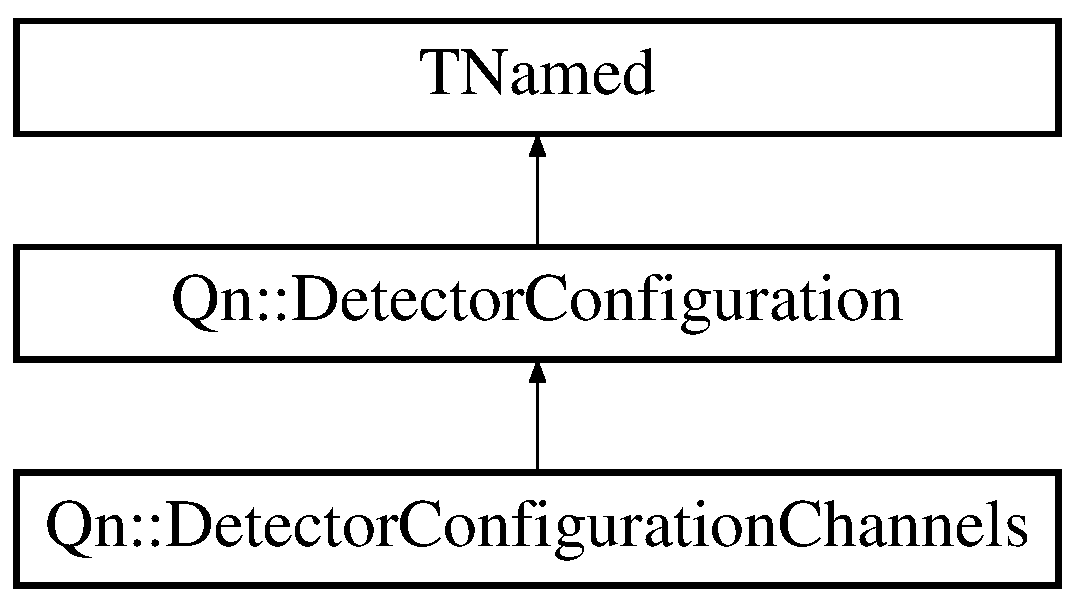
\includegraphics[height=3.000000cm]{classQn_1_1DetectorConfigurationChannels}
\end{center}
\end{figure}
\subsection*{Public Member Functions}
\begin{DoxyCompactItemize}
\item 
\mbox{\Hypertarget{classQn_1_1DetectorConfigurationChannels_a4db2660fe522de2dc67222f7c3900662}\label{classQn_1_1DetectorConfigurationChannels_a4db2660fe522de2dc67222f7c3900662}} 
\mbox{\hyperlink{classQn_1_1DetectorConfigurationChannels_a4db2660fe522de2dc67222f7c3900662}{Detector\+Configuration\+Channels}} ()
\begin{DoxyCompactList}\small\item\em Default constructor. \end{DoxyCompactList}\item 
\mbox{\hyperlink{classQn_1_1DetectorConfigurationChannels_a317ef35a90228d567c1ba612476e6730}{Detector\+Configuration\+Channels}} (const char $\ast$name, \mbox{\hyperlink{classQn_1_1EventClassVariablesSet}{Event\+Class\+Variables\+Set}} $\ast$event\+Classes\+Variables, Int\+\_\+t n\+No\+Of\+Channels, Int\+\_\+t n\+No\+Of\+Harmonics, Int\+\_\+t $\ast$harmonic\+Map=N\+U\+LL)
\item 
virtual \mbox{\hyperlink{classQn_1_1DetectorConfigurationChannels_aeb451a1ee7e9444dde635d2bb11dafd3}{$\sim$\+Detector\+Configuration\+Channels}} ()
\item 
Int\+\_\+t \mbox{\hyperlink{classQn_1_1DetectorConfigurationChannels_a7d31f3204016bbb12099911649c29840}{Get\+No\+Of\+Channels}} ()
\item 
const Bool\+\_\+t $\ast$ \mbox{\hyperlink{classQn_1_1DetectorConfigurationChannels_a541ac77e7e2e15690eed089a66d0c5a1}{Get\+Used\+Channels\+Mask}} () const
\item 
const Int\+\_\+t $\ast$ \mbox{\hyperlink{classQn_1_1DetectorConfigurationChannels_a393356a54937b18706b49b3e6748674f}{Get\+Channels\+Groups}} () const
\item 
const Float\+\_\+t $\ast$ \mbox{\hyperlink{classQn_1_1DetectorConfigurationChannels_a7de674ab1e919b85391215c18db325ca}{Get\+Hard\+Coded\+Group\+Weights}} () const
\item 
virtual Bool\+\_\+t \mbox{\hyperlink{classQn_1_1DetectorConfigurationChannels_a24728cc5b3b9f80f9965268d1153f06c}{Get\+Is\+Tracking\+Detector}} () const
\item 
virtual void \mbox{\hyperlink{classQn_1_1DetectorConfigurationChannels_a920171069e4f5e36e0849cc5ac3c9a3d}{Set\+Channels\+Scheme}} (Bool\+\_\+t $\ast$b\+Used\+Channel, Int\+\_\+t $\ast$n\+Channel\+Group=nullptr, Float\+\_\+t $\ast$hard\+Coded\+Group\+Weights=nullptr)
\item 
void \mbox{\hyperlink{classQn_1_1DetectorConfigurationChannels_ad7d7c25a2940f842783863ebf9a59fad}{Set\+Q\+A\+Centrality\+Var}} (Int\+\_\+t id)
\item 
void \mbox{\hyperlink{classQn_1_1DetectorConfigurationChannels_aaddda392786336026b2e91fb9d26a733}{Set\+Q\+A\+Multiplicity\+Axis}} (Int\+\_\+t nbins, Float\+\_\+t min, Float\+\_\+t max)
\item 
virtual void \mbox{\hyperlink{classQn_1_1DetectorConfigurationChannels_a074acfba4bc0d41df71d53b98d682f57}{Attach\+Corrections\+Manager}} (\mbox{\hyperlink{classQn_1_1CorrectionCalculator}{Correction\+Calculator}} $\ast$manager)
\item 
virtual void \mbox{\hyperlink{classQn_1_1DetectorConfigurationChannels_ab19e6fe4c194060859eef7941b1c716c}{Create\+Support\+Data\+Structures}} ()
\item 
virtual Bool\+\_\+t \mbox{\hyperlink{classQn_1_1DetectorConfigurationChannels_a68e68df13b56e3e9f55adc8cae0a505d}{Create\+Support\+Histograms}} (T\+List $\ast$list)
\item 
virtual Bool\+\_\+t \mbox{\hyperlink{classQn_1_1DetectorConfigurationChannels_a0e3a0e4775decda04c3bad48534c297a}{Create\+Q\+A\+Histograms}} (T\+List $\ast$list)
\item 
virtual Bool\+\_\+t \mbox{\hyperlink{classQn_1_1DetectorConfigurationChannels_a62452177f5059e64977c5c1fc079de0b}{Create\+Nve\+Q\+A\+Histograms}} (T\+List $\ast$list)
\item 
virtual void \mbox{\hyperlink{classQn_1_1DetectorConfigurationChannels_a6e0cb5f19763dd57e017325d456adb39}{Activate\+Harmonic}} (Int\+\_\+t harmonic)
\item 
virtual Bool\+\_\+t \mbox{\hyperlink{classQn_1_1DetectorConfigurationChannels_ac02f3bf7815650e06a3b85f3c0bcd0e0}{Attach\+Correction\+Inputs}} (T\+List $\ast$list)
\item 
virtual void \mbox{\hyperlink{classQn_1_1DetectorConfigurationChannels_aee41ab7c778ea075aa7e4f414c8817e0}{After\+Inputs\+Attach\+Actions}} ()
\item 
virtual Bool\+\_\+t \mbox{\hyperlink{classQn_1_1DetectorConfigurationChannels_a327a2d868d9cc1596e83f54354c3df44}{Process\+Corrections}} (const double $\ast$variable\+Container)
\item 
virtual Bool\+\_\+t \mbox{\hyperlink{classQn_1_1DetectorConfigurationChannels_a972f2cc50810d2a9651f2920de5a03ec}{Process\+Data\+Collection}} (const double $\ast$variable\+Container)
\item 
virtual void \mbox{\hyperlink{classQn_1_1DetectorConfigurationChannels_ab5c641503809ce981651bb08ffc50f0e}{Add\+Correction\+On\+Input\+Data}} (\mbox{\hyperlink{classQn_1_1CorrectionOnInputData}{Correction\+On\+Input\+Data}} $\ast$correction\+On\+Input\+Data)
\item 
virtual Bool\+\_\+t \mbox{\hyperlink{classQn_1_1DetectorConfigurationChannels_a1f22484e703888f5ff9548d9a8421d3b}{Add\+Data\+Vector}} (const double $\ast$variable\+Container, Double\+\_\+t phi, Double\+\_\+t weight, Int\+\_\+t channel\+Id)
\item 
virtual void \mbox{\hyperlink{classQn_1_1DetectorConfigurationChannels_aa68804ba67cf6fdee8891e6aed0e14f7}{Build\+Qn\+Vector}} ()
\item 
void \mbox{\hyperlink{classQn_1_1DetectorConfigurationChannels_a6770ab3360c5e688c30bbea0522f3856}{Build\+Raw\+Qn\+Vector}} ()
\item 
virtual void \mbox{\hyperlink{classQn_1_1DetectorConfigurationChannels_a6756b2b2bed25bee5659953ae82ce5b7}{Include\+Qn\+Vectors}} (T\+List $\ast$list)
\item 
virtual void \mbox{\hyperlink{classQn_1_1DetectorConfigurationChannels_aa9e99a908719d0de616cebf9329fe83f}{Fill\+Overall\+Input\+Correction\+Step\+List}} (T\+List $\ast$list) const
\item 
virtual void \mbox{\hyperlink{classQn_1_1DetectorConfigurationChannels_a002931544421b46c9402aa7bdefcff51}{Fill\+Overall\+Qn\+Vector\+Correction\+Step\+List}} (T\+List $\ast$list) const
\item 
virtual void \mbox{\hyperlink{classQn_1_1DetectorConfigurationChannels_a753f23bd918444d853d1deebeefa4727}{Report\+On\+Corrections}} (T\+List $\ast$steps, T\+List $\ast$calib, T\+List $\ast$apply) const
\item 
virtual Bool\+\_\+t \mbox{\hyperlink{classQn_1_1DetectorConfigurationChannels_a45d03a27b4825709c2440a905ca8959a}{Is\+Selected}} (const double $\ast$variable\+Container, Int\+\_\+t n\+Channel)
\item 
\mbox{\Hypertarget{classQn_1_1DetectorConfigurationChannels_afa63699a8f8dad1d2506b607f1ed8e83}\label{classQn_1_1DetectorConfigurationChannels_afa63699a8f8dad1d2506b607f1ed8e83}} 
virtual Bool\+\_\+t \mbox{\hyperlink{classQn_1_1DetectorConfigurationChannels_afa63699a8f8dad1d2506b607f1ed8e83}{Is\+Selected}} (const double $\ast$variable\+Container)
\begin{DoxyCompactList}\small\item\em wrong call for this class invoke base class behavior \end{DoxyCompactList}\item 
virtual void \mbox{\hyperlink{classQn_1_1DetectorConfigurationChannels_a692b4880a3a694cf9a3ad860cb3f7b52}{Clear\+Configuration}} ()
\end{DoxyCompactItemize}
\subsection*{Friends}
\begin{DoxyCompactItemize}
\item 
\mbox{\Hypertarget{classQn_1_1DetectorConfigurationChannels_afbb351f0a159c2e61159977b03f4b3c1}\label{classQn_1_1DetectorConfigurationChannels_afbb351f0a159c2e61159977b03f4b3c1}} 
class {\bfseries Correction\+Step\+Base}
\item 
\mbox{\Hypertarget{classQn_1_1DetectorConfigurationChannels_aaaec1af05216df7a0fa18215ef18023b}\label{classQn_1_1DetectorConfigurationChannels_aaaec1af05216df7a0fa18215ef18023b}} 
class {\bfseries Correction\+Detector}
\end{DoxyCompactItemize}
\subsection*{Additional Inherited Members}


\subsection{Constructor \& Destructor Documentation}
\mbox{\Hypertarget{classQn_1_1DetectorConfigurationChannels_a317ef35a90228d567c1ba612476e6730}\label{classQn_1_1DetectorConfigurationChannels_a317ef35a90228d567c1ba612476e6730}} 
\index{Qn\+::\+Detector\+Configuration\+Channels@{Qn\+::\+Detector\+Configuration\+Channels}!Detector\+Configuration\+Channels@{Detector\+Configuration\+Channels}}
\index{Detector\+Configuration\+Channels@{Detector\+Configuration\+Channels}!Qn\+::\+Detector\+Configuration\+Channels@{Qn\+::\+Detector\+Configuration\+Channels}}
\subsubsection{\texorpdfstring{Detector\+Configuration\+Channels()}{DetectorConfigurationChannels()}}
{\footnotesize\ttfamily Qn\+::\+Detector\+Configuration\+Channels\+::\+Detector\+Configuration\+Channels (\begin{DoxyParamCaption}\item[{const char $\ast$}]{name,  }\item[{\mbox{\hyperlink{classQn_1_1EventClassVariablesSet}{Event\+Class\+Variables\+Set}} $\ast$}]{event\+Classes\+Variables,  }\item[{Int\+\_\+t}]{n\+No\+Of\+Channels,  }\item[{Int\+\_\+t}]{n\+No\+Of\+Harmonics,  }\item[{Int\+\_\+t $\ast$}]{harmonic\+Map = {\ttfamily NULL} }\end{DoxyParamCaption})}

Normal constructor Allocates the data vector bank. 
\begin{DoxyParams}{Parameters}
{\em name} & the name of the detector configuration \\
\hline
{\em event\+Classes\+Variables} & the set of event classes variables \\
\hline
{\em n\+No\+Of\+Channels} & the number of channels of the associated detector \\
\hline
{\em n\+No\+Of\+Harmonics} & the number of harmonics that must be handled \\
\hline
{\em harmonic\+Map} & an optional ordered array with the harmonic numbers \\
\hline
\end{DoxyParams}
\mbox{\Hypertarget{classQn_1_1DetectorConfigurationChannels_aeb451a1ee7e9444dde635d2bb11dafd3}\label{classQn_1_1DetectorConfigurationChannels_aeb451a1ee7e9444dde635d2bb11dafd3}} 
\index{Qn\+::\+Detector\+Configuration\+Channels@{Qn\+::\+Detector\+Configuration\+Channels}!````~Detector\+Configuration\+Channels@{$\sim$\+Detector\+Configuration\+Channels}}
\index{````~Detector\+Configuration\+Channels@{$\sim$\+Detector\+Configuration\+Channels}!Qn\+::\+Detector\+Configuration\+Channels@{Qn\+::\+Detector\+Configuration\+Channels}}
\subsubsection{\texorpdfstring{$\sim$\+Detector\+Configuration\+Channels()}{~DetectorConfigurationChannels()}}
{\footnotesize\ttfamily Qn\+::\+Detector\+Configuration\+Channels\+::$\sim$\+Detector\+Configuration\+Channels (\begin{DoxyParamCaption}{ }\end{DoxyParamCaption})\hspace{0.3cm}{\ttfamily [virtual]}}

Default destructor Releases the memory taken 

\subsection{Member Function Documentation}
\mbox{\Hypertarget{classQn_1_1DetectorConfigurationChannels_a6e0cb5f19763dd57e017325d456adb39}\label{classQn_1_1DetectorConfigurationChannels_a6e0cb5f19763dd57e017325d456adb39}} 
\index{Qn\+::\+Detector\+Configuration\+Channels@{Qn\+::\+Detector\+Configuration\+Channels}!Activate\+Harmonic@{Activate\+Harmonic}}
\index{Activate\+Harmonic@{Activate\+Harmonic}!Qn\+::\+Detector\+Configuration\+Channels@{Qn\+::\+Detector\+Configuration\+Channels}}
\subsubsection{\texorpdfstring{Activate\+Harmonic()}{ActivateHarmonic()}}
{\footnotesize\ttfamily virtual void Qn\+::\+Detector\+Configuration\+Channels\+::\+Activate\+Harmonic (\begin{DoxyParamCaption}\item[{Int\+\_\+t}]{harmonic }\end{DoxyParamCaption})\hspace{0.3cm}{\ttfamily [inline]}, {\ttfamily [virtual]}}

Activate the processing for the passed harmonic 
\begin{DoxyParams}{Parameters}
{\em harmonic} & the desired harmonic number to activate \\
\hline
\end{DoxyParams}


Reimplemented from \mbox{\hyperlink{classQn_1_1DetectorConfiguration_a5bb71f7e186c058cad8c6bba4f2596cd}{Qn\+::\+Detector\+Configuration}}.

\mbox{\Hypertarget{classQn_1_1DetectorConfigurationChannels_ab5c641503809ce981651bb08ffc50f0e}\label{classQn_1_1DetectorConfigurationChannels_ab5c641503809ce981651bb08ffc50f0e}} 
\index{Qn\+::\+Detector\+Configuration\+Channels@{Qn\+::\+Detector\+Configuration\+Channels}!Add\+Correction\+On\+Input\+Data@{Add\+Correction\+On\+Input\+Data}}
\index{Add\+Correction\+On\+Input\+Data@{Add\+Correction\+On\+Input\+Data}!Qn\+::\+Detector\+Configuration\+Channels@{Qn\+::\+Detector\+Configuration\+Channels}}
\subsubsection{\texorpdfstring{Add\+Correction\+On\+Input\+Data()}{AddCorrectionOnInputData()}}
{\footnotesize\ttfamily void Qn\+::\+Detector\+Configuration\+Channels\+::\+Add\+Correction\+On\+Input\+Data (\begin{DoxyParamCaption}\item[{\mbox{\hyperlink{classQn_1_1CorrectionOnInputData}{Correction\+On\+Input\+Data}} $\ast$}]{correction\+On\+Input\+Data }\end{DoxyParamCaption})\hspace{0.3cm}{\ttfamily [virtual]}}

Incorporates the passed correction to the set of input data corrections 
\begin{DoxyParams}{Parameters}
{\em correction\+On\+Input\+Data} & the correction to add \\
\hline
\end{DoxyParams}


Reimplemented from \mbox{\hyperlink{classQn_1_1DetectorConfiguration_ab65571f46d348c2b07d3b03fc1e6cf11}{Qn\+::\+Detector\+Configuration}}.

\mbox{\Hypertarget{classQn_1_1DetectorConfigurationChannels_a1f22484e703888f5ff9548d9a8421d3b}\label{classQn_1_1DetectorConfigurationChannels_a1f22484e703888f5ff9548d9a8421d3b}} 
\index{Qn\+::\+Detector\+Configuration\+Channels@{Qn\+::\+Detector\+Configuration\+Channels}!Add\+Data\+Vector@{Add\+Data\+Vector}}
\index{Add\+Data\+Vector@{Add\+Data\+Vector}!Qn\+::\+Detector\+Configuration\+Channels@{Qn\+::\+Detector\+Configuration\+Channels}}
\subsubsection{\texorpdfstring{Add\+Data\+Vector()}{AddDataVector()}}
{\footnotesize\ttfamily Bool\+\_\+t Qn\+::\+Detector\+Configuration\+Channels\+::\+Add\+Data\+Vector (\begin{DoxyParamCaption}\item[{const double $\ast$}]{variable\+Container,  }\item[{Double\+\_\+t}]{phi,  }\item[{Double\+\_\+t}]{weight,  }\item[{Int\+\_\+t}]{channel\+Id }\end{DoxyParamCaption})\hspace{0.3cm}{\ttfamily [inline]}, {\ttfamily [virtual]}}

New data vector for the detector configuration. A check is made to match the channel Id with the ones assigned to the detector configuration and then an additional one to see if the current variable bank content passes the associated cuts. If so, the data vector is stored. 
\begin{DoxyParams}{Parameters}
{\em variable\+Container} & pointer to the variable content bank \\
\hline
{\em phi} & azimuthal angle \\
\hline
{\em weight} & the weight of the data vector. Ignored for track detector configurations. \\
\hline
{\em channel\+Id} & the channel Id that originates the data vector. Ignored for track detector configurations. \\
\hline
\end{DoxyParams}
\begin{DoxyReturn}{Returns}
k\+T\+R\+UE if the data vector was accepted and stored 
\end{DoxyReturn}
add the data vector to the bank 

Implements \mbox{\hyperlink{classQn_1_1DetectorConfiguration_ab406e0d2a85e7f5a7c74d0bd0252375d}{Qn\+::\+Detector\+Configuration}}.

\mbox{\Hypertarget{classQn_1_1DetectorConfigurationChannels_aee41ab7c778ea075aa7e4f414c8817e0}\label{classQn_1_1DetectorConfigurationChannels_aee41ab7c778ea075aa7e4f414c8817e0}} 
\index{Qn\+::\+Detector\+Configuration\+Channels@{Qn\+::\+Detector\+Configuration\+Channels}!After\+Inputs\+Attach\+Actions@{After\+Inputs\+Attach\+Actions}}
\index{After\+Inputs\+Attach\+Actions@{After\+Inputs\+Attach\+Actions}!Qn\+::\+Detector\+Configuration\+Channels@{Qn\+::\+Detector\+Configuration\+Channels}}
\subsubsection{\texorpdfstring{After\+Inputs\+Attach\+Actions()}{AfterInputsAttachActions()}}
{\footnotesize\ttfamily void Qn\+::\+Detector\+Configuration\+Channels\+::\+After\+Inputs\+Attach\+Actions (\begin{DoxyParamCaption}{ }\end{DoxyParamCaption})\hspace{0.3cm}{\ttfamily [virtual]}}

Perform after calibration histograms attach actions It is used to inform the different correction step that all conditions for running the network are in place so it is time to check if their requirements are satisfied

The request is transmitted to the input data corrections and then propagated to the Q vector corrections 

Implements \mbox{\hyperlink{classQn_1_1DetectorConfiguration_ab6766905dffe5811aefa59dd1e1117d8}{Qn\+::\+Detector\+Configuration}}.

\mbox{\Hypertarget{classQn_1_1DetectorConfigurationChannels_ac02f3bf7815650e06a3b85f3c0bcd0e0}\label{classQn_1_1DetectorConfigurationChannels_ac02f3bf7815650e06a3b85f3c0bcd0e0}} 
\index{Qn\+::\+Detector\+Configuration\+Channels@{Qn\+::\+Detector\+Configuration\+Channels}!Attach\+Correction\+Inputs@{Attach\+Correction\+Inputs}}
\index{Attach\+Correction\+Inputs@{Attach\+Correction\+Inputs}!Qn\+::\+Detector\+Configuration\+Channels@{Qn\+::\+Detector\+Configuration\+Channels}}
\subsubsection{\texorpdfstring{Attach\+Correction\+Inputs()}{AttachCorrectionInputs()}}
{\footnotesize\ttfamily Bool\+\_\+t Qn\+::\+Detector\+Configuration\+Channels\+::\+Attach\+Correction\+Inputs (\begin{DoxyParamCaption}\item[{T\+List $\ast$}]{list }\end{DoxyParamCaption})\hspace{0.3cm}{\ttfamily [virtual]}}

Asks for attaching the needed input information to the correction steps

The detector list is extracted from the passed list and then the request is transmitted to the input data corrections and then propagated to the Q vector corrections 
\begin{DoxyParams}{Parameters}
{\em list} & list where the input information should be found \\
\hline
\end{DoxyParams}
\begin{DoxyReturn}{Returns}
k\+T\+R\+UE if everything went OK 
\end{DoxyReturn}


Implements \mbox{\hyperlink{classQn_1_1DetectorConfiguration_a4ae0eb587070e68a11fbb438d96fca15}{Qn\+::\+Detector\+Configuration}}.

\mbox{\Hypertarget{classQn_1_1DetectorConfigurationChannels_a074acfba4bc0d41df71d53b98d682f57}\label{classQn_1_1DetectorConfigurationChannels_a074acfba4bc0d41df71d53b98d682f57}} 
\index{Qn\+::\+Detector\+Configuration\+Channels@{Qn\+::\+Detector\+Configuration\+Channels}!Attach\+Corrections\+Manager@{Attach\+Corrections\+Manager}}
\index{Attach\+Corrections\+Manager@{Attach\+Corrections\+Manager}!Qn\+::\+Detector\+Configuration\+Channels@{Qn\+::\+Detector\+Configuration\+Channels}}
\subsubsection{\texorpdfstring{Attach\+Corrections\+Manager()}{AttachCorrectionsManager()}}
{\footnotesize\ttfamily void Qn\+::\+Detector\+Configuration\+Channels\+::\+Attach\+Corrections\+Manager (\begin{DoxyParamCaption}\item[{\mbox{\hyperlink{classQn_1_1CorrectionCalculator}{Correction\+Calculator}} $\ast$}]{manager }\end{DoxyParamCaption})\hspace{0.3cm}{\ttfamily [virtual]}}

Stores the framework manager pointer Orders the base class to store the correction manager and informs the input data corrections and the \mbox{\hyperlink{namespaceQn}{Qn}} vector corrections they are now attached to the framework 
\begin{DoxyParams}{Parameters}
{\em manager} & the framework manager \\
\hline
\end{DoxyParams}


Implements \mbox{\hyperlink{classQn_1_1DetectorConfiguration_a512c77d73e0e6453607f7ae7e2e8f72b}{Qn\+::\+Detector\+Configuration}}.

\mbox{\Hypertarget{classQn_1_1DetectorConfigurationChannels_aa68804ba67cf6fdee8891e6aed0e14f7}\label{classQn_1_1DetectorConfigurationChannels_aa68804ba67cf6fdee8891e6aed0e14f7}} 
\index{Qn\+::\+Detector\+Configuration\+Channels@{Qn\+::\+Detector\+Configuration\+Channels}!Build\+Qn\+Vector@{Build\+Qn\+Vector}}
\index{Build\+Qn\+Vector@{Build\+Qn\+Vector}!Qn\+::\+Detector\+Configuration\+Channels@{Qn\+::\+Detector\+Configuration\+Channels}}
\subsubsection{\texorpdfstring{Build\+Qn\+Vector()}{BuildQnVector()}}
{\footnotesize\ttfamily void Qn\+::\+Detector\+Configuration\+Channels\+::\+Build\+Qn\+Vector (\begin{DoxyParamCaption}{ }\end{DoxyParamCaption})\hspace{0.3cm}{\ttfamily [inline]}, {\ttfamily [virtual]}}

Builds \mbox{\hyperlink{namespaceQn}{Qn}} vector before Q vector corrections and after input corrections and considering the chosen calibration method. The built Q vector is the one to be used for subsequent Q vector corrections. 

Implements \mbox{\hyperlink{classQn_1_1DetectorConfiguration_a7aaf10f6e30151dd142d59d5dff72e2d}{Qn\+::\+Detector\+Configuration}}.

\mbox{\Hypertarget{classQn_1_1DetectorConfigurationChannels_a6770ab3360c5e688c30bbea0522f3856}\label{classQn_1_1DetectorConfigurationChannels_a6770ab3360c5e688c30bbea0522f3856}} 
\index{Qn\+::\+Detector\+Configuration\+Channels@{Qn\+::\+Detector\+Configuration\+Channels}!Build\+Raw\+Qn\+Vector@{Build\+Raw\+Qn\+Vector}}
\index{Build\+Raw\+Qn\+Vector@{Build\+Raw\+Qn\+Vector}!Qn\+::\+Detector\+Configuration\+Channels@{Qn\+::\+Detector\+Configuration\+Channels}}
\subsubsection{\texorpdfstring{Build\+Raw\+Qn\+Vector()}{BuildRawQnVector()}}
{\footnotesize\ttfamily void Qn\+::\+Detector\+Configuration\+Channels\+::\+Build\+Raw\+Qn\+Vector (\begin{DoxyParamCaption}{ }\end{DoxyParamCaption})\hspace{0.3cm}{\ttfamily [inline]}}

Builds raw \mbox{\hyperlink{namespaceQn}{Qn}} vector before Q vector corrections and before input data corrections but considering the chosen calibration method. This is a channelized configuration so this Q vector will N\+OT be the one to be used for subsequent Q vector corrections. \mbox{\Hypertarget{classQn_1_1DetectorConfigurationChannels_a692b4880a3a694cf9a3ad860cb3f7b52}\label{classQn_1_1DetectorConfigurationChannels_a692b4880a3a694cf9a3ad860cb3f7b52}} 
\index{Qn\+::\+Detector\+Configuration\+Channels@{Qn\+::\+Detector\+Configuration\+Channels}!Clear\+Configuration@{Clear\+Configuration}}
\index{Clear\+Configuration@{Clear\+Configuration}!Qn\+::\+Detector\+Configuration\+Channels@{Qn\+::\+Detector\+Configuration\+Channels}}
\subsubsection{\texorpdfstring{Clear\+Configuration()}{ClearConfiguration()}}
{\footnotesize\ttfamily void Qn\+::\+Detector\+Configuration\+Channels\+::\+Clear\+Configuration (\begin{DoxyParamCaption}{ }\end{DoxyParamCaption})\hspace{0.3cm}{\ttfamily [inline]}, {\ttfamily [virtual]}}

Clean the configuration to accept a new event

Transfers the order to the Q vector correction steps then to the input data correction steps and finally cleans the own Q vector and the input data vector bank for accepting the next event. 

Implements \mbox{\hyperlink{classQn_1_1DetectorConfiguration_a94c21b39a4a3680675319aacf4a517f4}{Qn\+::\+Detector\+Configuration}}.

\mbox{\Hypertarget{classQn_1_1DetectorConfigurationChannels_a62452177f5059e64977c5c1fc079de0b}\label{classQn_1_1DetectorConfigurationChannels_a62452177f5059e64977c5c1fc079de0b}} 
\index{Qn\+::\+Detector\+Configuration\+Channels@{Qn\+::\+Detector\+Configuration\+Channels}!Create\+Nve\+Q\+A\+Histograms@{Create\+Nve\+Q\+A\+Histograms}}
\index{Create\+Nve\+Q\+A\+Histograms@{Create\+Nve\+Q\+A\+Histograms}!Qn\+::\+Detector\+Configuration\+Channels@{Qn\+::\+Detector\+Configuration\+Channels}}
\subsubsection{\texorpdfstring{Create\+Nve\+Q\+A\+Histograms()}{CreateNveQAHistograms()}}
{\footnotesize\ttfamily Bool\+\_\+t Qn\+::\+Detector\+Configuration\+Channels\+::\+Create\+Nve\+Q\+A\+Histograms (\begin{DoxyParamCaption}\item[{T\+List $\ast$}]{list }\end{DoxyParamCaption})\hspace{0.3cm}{\ttfamily [virtual]}}

Asks for non validated entries QA histograms creation

A new histograms list is created for the detector and incorporated to the passed list. Then the new list is passed first to the input data corrections and then to the Q vector corrections. 
\begin{DoxyParams}{Parameters}
{\em list} & list where the histograms should be incorporated for its persistence \\
\hline
\end{DoxyParams}
\begin{DoxyReturn}{Returns}
k\+T\+R\+UE if everything went OK 
\end{DoxyReturn}


Implements \mbox{\hyperlink{classQn_1_1DetectorConfiguration_ade61875d8e7a05dd413c94d6887ae4ac}{Qn\+::\+Detector\+Configuration}}.

\mbox{\Hypertarget{classQn_1_1DetectorConfigurationChannels_a0e3a0e4775decda04c3bad48534c297a}\label{classQn_1_1DetectorConfigurationChannels_a0e3a0e4775decda04c3bad48534c297a}} 
\index{Qn\+::\+Detector\+Configuration\+Channels@{Qn\+::\+Detector\+Configuration\+Channels}!Create\+Q\+A\+Histograms@{Create\+Q\+A\+Histograms}}
\index{Create\+Q\+A\+Histograms@{Create\+Q\+A\+Histograms}!Qn\+::\+Detector\+Configuration\+Channels@{Qn\+::\+Detector\+Configuration\+Channels}}
\subsubsection{\texorpdfstring{Create\+Q\+A\+Histograms()}{CreateQAHistograms()}}
{\footnotesize\ttfamily Bool\+\_\+t Qn\+::\+Detector\+Configuration\+Channels\+::\+Create\+Q\+A\+Histograms (\begin{DoxyParamCaption}\item[{T\+List $\ast$}]{list }\end{DoxyParamCaption})\hspace{0.3cm}{\ttfamily [virtual]}}

Asks for QA histograms creation

A new histograms list is created for the detector and incorporated to the passed list. The own QA histograms are then created and incorporated to the new list. Then the new list is passed first to the input data corrections and then to the Q vector corrections. 
\begin{DoxyParams}{Parameters}
{\em list} & list where the histograms should be incorporated for its persistence \\
\hline
\end{DoxyParams}
\begin{DoxyReturn}{Returns}
k\+T\+R\+UE if everything went OK 
\end{DoxyReturn}


Implements \mbox{\hyperlink{classQn_1_1DetectorConfiguration_a9f527d4c584e6bd79b6b8eb0b7f5413a}{Qn\+::\+Detector\+Configuration}}.

\mbox{\Hypertarget{classQn_1_1DetectorConfigurationChannels_ab19e6fe4c194060859eef7941b1c716c}\label{classQn_1_1DetectorConfigurationChannels_ab19e6fe4c194060859eef7941b1c716c}} 
\index{Qn\+::\+Detector\+Configuration\+Channels@{Qn\+::\+Detector\+Configuration\+Channels}!Create\+Support\+Data\+Structures@{Create\+Support\+Data\+Structures}}
\index{Create\+Support\+Data\+Structures@{Create\+Support\+Data\+Structures}!Qn\+::\+Detector\+Configuration\+Channels@{Qn\+::\+Detector\+Configuration\+Channels}}
\subsubsection{\texorpdfstring{Create\+Support\+Data\+Structures()}{CreateSupportDataStructures()}}
{\footnotesize\ttfamily void Qn\+::\+Detector\+Configuration\+Channels\+::\+Create\+Support\+Data\+Structures (\begin{DoxyParamCaption}{ }\end{DoxyParamCaption})\hspace{0.3cm}{\ttfamily [virtual]}}

Asks for support data structures creation

The input data vector bank is allocated and the request is transmitted to the input data corrections and then to the Q vector corrections. 

Implements \mbox{\hyperlink{classQn_1_1DetectorConfiguration_a664f65925f22f8f02c1a216f77b533ce}{Qn\+::\+Detector\+Configuration}}.

\mbox{\Hypertarget{classQn_1_1DetectorConfigurationChannels_a68e68df13b56e3e9f55adc8cae0a505d}\label{classQn_1_1DetectorConfigurationChannels_a68e68df13b56e3e9f55adc8cae0a505d}} 
\index{Qn\+::\+Detector\+Configuration\+Channels@{Qn\+::\+Detector\+Configuration\+Channels}!Create\+Support\+Histograms@{Create\+Support\+Histograms}}
\index{Create\+Support\+Histograms@{Create\+Support\+Histograms}!Qn\+::\+Detector\+Configuration\+Channels@{Qn\+::\+Detector\+Configuration\+Channels}}
\subsubsection{\texorpdfstring{Create\+Support\+Histograms()}{CreateSupportHistograms()}}
{\footnotesize\ttfamily Bool\+\_\+t Qn\+::\+Detector\+Configuration\+Channels\+::\+Create\+Support\+Histograms (\begin{DoxyParamCaption}\item[{T\+List $\ast$}]{list }\end{DoxyParamCaption})\hspace{0.3cm}{\ttfamily [virtual]}}

Asks for support histograms creation

A new histograms list is created for the detector and incorporated to the passed list. Then the new list is passed first to the input data corrections and then to the Q vector corrections. 
\begin{DoxyParams}{Parameters}
{\em list} & list where the histograms should be incorporated for its persistence \\
\hline
\end{DoxyParams}
\begin{DoxyReturn}{Returns}
k\+T\+R\+UE if everything went OK 
\end{DoxyReturn}


Implements \mbox{\hyperlink{classQn_1_1DetectorConfiguration_a8e5e2eef94bca58a3dcf34fe5fbd1429}{Qn\+::\+Detector\+Configuration}}.

\mbox{\Hypertarget{classQn_1_1DetectorConfigurationChannels_aa9e99a908719d0de616cebf9329fe83f}\label{classQn_1_1DetectorConfigurationChannels_aa9e99a908719d0de616cebf9329fe83f}} 
\index{Qn\+::\+Detector\+Configuration\+Channels@{Qn\+::\+Detector\+Configuration\+Channels}!Fill\+Overall\+Input\+Correction\+Step\+List@{Fill\+Overall\+Input\+Correction\+Step\+List}}
\index{Fill\+Overall\+Input\+Correction\+Step\+List@{Fill\+Overall\+Input\+Correction\+Step\+List}!Qn\+::\+Detector\+Configuration\+Channels@{Qn\+::\+Detector\+Configuration\+Channels}}
\subsubsection{\texorpdfstring{Fill\+Overall\+Input\+Correction\+Step\+List()}{FillOverallInputCorrectionStepList()}}
{\footnotesize\ttfamily void Qn\+::\+Detector\+Configuration\+Channels\+::\+Fill\+Overall\+Input\+Correction\+Step\+List (\begin{DoxyParamCaption}\item[{T\+List $\ast$}]{list }\end{DoxyParamCaption}) const\hspace{0.3cm}{\ttfamily [virtual]}}

Include only one instance of each input correction step in execution order

The request is transmitted to the set of \mbox{\hyperlink{namespaceQn}{Qn}} vector corrections 
\begin{DoxyParams}{Parameters}
{\em list} & list where the correction steps should be incorporated \\
\hline
\end{DoxyParams}


Implements \mbox{\hyperlink{classQn_1_1DetectorConfiguration_a76e173f938b886b5575597d9464698b4}{Qn\+::\+Detector\+Configuration}}.

\mbox{\Hypertarget{classQn_1_1DetectorConfigurationChannels_a002931544421b46c9402aa7bdefcff51}\label{classQn_1_1DetectorConfigurationChannels_a002931544421b46c9402aa7bdefcff51}} 
\index{Qn\+::\+Detector\+Configuration\+Channels@{Qn\+::\+Detector\+Configuration\+Channels}!Fill\+Overall\+Qn\+Vector\+Correction\+Step\+List@{Fill\+Overall\+Qn\+Vector\+Correction\+Step\+List}}
\index{Fill\+Overall\+Qn\+Vector\+Correction\+Step\+List@{Fill\+Overall\+Qn\+Vector\+Correction\+Step\+List}!Qn\+::\+Detector\+Configuration\+Channels@{Qn\+::\+Detector\+Configuration\+Channels}}
\subsubsection{\texorpdfstring{Fill\+Overall\+Qn\+Vector\+Correction\+Step\+List()}{FillOverallQnVectorCorrectionStepList()}}
{\footnotesize\ttfamily void Qn\+::\+Detector\+Configuration\+Channels\+::\+Fill\+Overall\+Qn\+Vector\+Correction\+Step\+List (\begin{DoxyParamCaption}\item[{T\+List $\ast$}]{list }\end{DoxyParamCaption}) const\hspace{0.3cm}{\ttfamily [virtual]}}

Include only one instance of each \mbox{\hyperlink{namespaceQn}{Qn}} vector correction step in execution order

The request is transmitted to the set of \mbox{\hyperlink{namespaceQn}{Qn}} vector corrections 
\begin{DoxyParams}{Parameters}
{\em list} & list where the correction steps should be incorporated \\
\hline
\end{DoxyParams}


Implements \mbox{\hyperlink{classQn_1_1DetectorConfiguration_ad71d83a2b0a5cee45bde15e936843e49}{Qn\+::\+Detector\+Configuration}}.

\mbox{\Hypertarget{classQn_1_1DetectorConfigurationChannels_a393356a54937b18706b49b3e6748674f}\label{classQn_1_1DetectorConfigurationChannels_a393356a54937b18706b49b3e6748674f}} 
\index{Qn\+::\+Detector\+Configuration\+Channels@{Qn\+::\+Detector\+Configuration\+Channels}!Get\+Channels\+Groups@{Get\+Channels\+Groups}}
\index{Get\+Channels\+Groups@{Get\+Channels\+Groups}!Qn\+::\+Detector\+Configuration\+Channels@{Qn\+::\+Detector\+Configuration\+Channels}}
\subsubsection{\texorpdfstring{Get\+Channels\+Groups()}{GetChannelsGroups()}}
{\footnotesize\ttfamily const Int\+\_\+t$\ast$ Qn\+::\+Detector\+Configuration\+Channels\+::\+Get\+Channels\+Groups (\begin{DoxyParamCaption}{ }\end{DoxyParamCaption}) const\hspace{0.3cm}{\ttfamily [inline]}}

Gets the channels groups \begin{DoxyReturn}{Returns}
the group associated to each channel 
\end{DoxyReturn}
\mbox{\Hypertarget{classQn_1_1DetectorConfigurationChannels_a7de674ab1e919b85391215c18db325ca}\label{classQn_1_1DetectorConfigurationChannels_a7de674ab1e919b85391215c18db325ca}} 
\index{Qn\+::\+Detector\+Configuration\+Channels@{Qn\+::\+Detector\+Configuration\+Channels}!Get\+Hard\+Coded\+Group\+Weights@{Get\+Hard\+Coded\+Group\+Weights}}
\index{Get\+Hard\+Coded\+Group\+Weights@{Get\+Hard\+Coded\+Group\+Weights}!Qn\+::\+Detector\+Configuration\+Channels@{Qn\+::\+Detector\+Configuration\+Channels}}
\subsubsection{\texorpdfstring{Get\+Hard\+Coded\+Group\+Weights()}{GetHardCodedGroupWeights()}}
{\footnotesize\ttfamily const Float\+\_\+t$\ast$ Qn\+::\+Detector\+Configuration\+Channels\+::\+Get\+Hard\+Coded\+Group\+Weights (\begin{DoxyParamCaption}{ }\end{DoxyParamCaption}) const\hspace{0.3cm}{\ttfamily [inline]}}

Gets the hard coded group weights \begin{DoxyReturn}{Returns}
the groups hard coded weights 
\end{DoxyReturn}
\mbox{\Hypertarget{classQn_1_1DetectorConfigurationChannels_a24728cc5b3b9f80f9965268d1153f06c}\label{classQn_1_1DetectorConfigurationChannels_a24728cc5b3b9f80f9965268d1153f06c}} 
\index{Qn\+::\+Detector\+Configuration\+Channels@{Qn\+::\+Detector\+Configuration\+Channels}!Get\+Is\+Tracking\+Detector@{Get\+Is\+Tracking\+Detector}}
\index{Get\+Is\+Tracking\+Detector@{Get\+Is\+Tracking\+Detector}!Qn\+::\+Detector\+Configuration\+Channels@{Qn\+::\+Detector\+Configuration\+Channels}}
\subsubsection{\texorpdfstring{Get\+Is\+Tracking\+Detector()}{GetIsTrackingDetector()}}
{\footnotesize\ttfamily virtual Bool\+\_\+t Qn\+::\+Detector\+Configuration\+Channels\+::\+Get\+Is\+Tracking\+Detector (\begin{DoxyParamCaption}{ }\end{DoxyParamCaption}) const\hspace{0.3cm}{\ttfamily [inline]}, {\ttfamily [virtual]}}

Get if the detector configuration is own by a tracking detector \begin{DoxyReturn}{Returns}
F\+A\+L\+SE, this is a hit / channel detector configuration 
\end{DoxyReturn}


Implements \mbox{\hyperlink{classQn_1_1DetectorConfiguration_acdb57db96ed24524b5a3a28821727a3d}{Qn\+::\+Detector\+Configuration}}.

\mbox{\Hypertarget{classQn_1_1DetectorConfigurationChannels_a7d31f3204016bbb12099911649c29840}\label{classQn_1_1DetectorConfigurationChannels_a7d31f3204016bbb12099911649c29840}} 
\index{Qn\+::\+Detector\+Configuration\+Channels@{Qn\+::\+Detector\+Configuration\+Channels}!Get\+No\+Of\+Channels@{Get\+No\+Of\+Channels}}
\index{Get\+No\+Of\+Channels@{Get\+No\+Of\+Channels}!Qn\+::\+Detector\+Configuration\+Channels@{Qn\+::\+Detector\+Configuration\+Channels}}
\subsubsection{\texorpdfstring{Get\+No\+Of\+Channels()}{GetNoOfChannels()}}
{\footnotesize\ttfamily Int\+\_\+t Qn\+::\+Detector\+Configuration\+Channels\+::\+Get\+No\+Of\+Channels (\begin{DoxyParamCaption}{ }\end{DoxyParamCaption})\hspace{0.3cm}{\ttfamily [inline]}}

Gets the number of channels \begin{DoxyReturn}{Returns}
the number of channels of the associated detector 
\end{DoxyReturn}
\mbox{\Hypertarget{classQn_1_1DetectorConfigurationChannels_a541ac77e7e2e15690eed089a66d0c5a1}\label{classQn_1_1DetectorConfigurationChannels_a541ac77e7e2e15690eed089a66d0c5a1}} 
\index{Qn\+::\+Detector\+Configuration\+Channels@{Qn\+::\+Detector\+Configuration\+Channels}!Get\+Used\+Channels\+Mask@{Get\+Used\+Channels\+Mask}}
\index{Get\+Used\+Channels\+Mask@{Get\+Used\+Channels\+Mask}!Qn\+::\+Detector\+Configuration\+Channels@{Qn\+::\+Detector\+Configuration\+Channels}}
\subsubsection{\texorpdfstring{Get\+Used\+Channels\+Mask()}{GetUsedChannelsMask()}}
{\footnotesize\ttfamily const Bool\+\_\+t$\ast$ Qn\+::\+Detector\+Configuration\+Channels\+::\+Get\+Used\+Channels\+Mask (\begin{DoxyParamCaption}{ }\end{DoxyParamCaption}) const\hspace{0.3cm}{\ttfamily [inline]}}

Gets the used channels mask \begin{DoxyReturn}{Returns}
the used channels mask 
\end{DoxyReturn}
\mbox{\Hypertarget{classQn_1_1DetectorConfigurationChannels_a6756b2b2bed25bee5659953ae82ce5b7}\label{classQn_1_1DetectorConfigurationChannels_a6756b2b2bed25bee5659953ae82ce5b7}} 
\index{Qn\+::\+Detector\+Configuration\+Channels@{Qn\+::\+Detector\+Configuration\+Channels}!Include\+Qn\+Vectors@{Include\+Qn\+Vectors}}
\index{Include\+Qn\+Vectors@{Include\+Qn\+Vectors}!Qn\+::\+Detector\+Configuration\+Channels@{Qn\+::\+Detector\+Configuration\+Channels}}
\subsubsection{\texorpdfstring{Include\+Qn\+Vectors()}{IncludeQnVectors()}}
{\footnotesize\ttfamily void Qn\+::\+Detector\+Configuration\+Channels\+::\+Include\+Qn\+Vectors (\begin{DoxyParamCaption}\item[{T\+List $\ast$}]{list }\end{DoxyParamCaption})\hspace{0.3cm}{\ttfamily [inline]}, {\ttfamily [virtual]}}

Include the the list of \mbox{\hyperlink{namespaceQn}{Qn}} vector associated to the detector configuration into the passed list

A new list is created for the detector configuration and incorporated to the passed list.

Always includes first the fully corrected \mbox{\hyperlink{namespaceQn}{Qn}} vector, and then includes the raw \mbox{\hyperlink{namespaceQn}{Qn}} vector and the plain \mbox{\hyperlink{namespaceQn}{Qn}} vector and then asks to the different correction steps to include their partially corrected \mbox{\hyperlink{namespaceQn}{Qn}} vectors.

The check if we are already there is because it could be late information about the process name and then the correction histograms could still not be attached and the constructed list does not contain the final \mbox{\hyperlink{namespaceQn}{Qn}} vectors. 
\begin{DoxyParams}{Parameters}
{\em list} & list where the corrected \mbox{\hyperlink{namespaceQn}{Qn}} vector should be added \\
\hline
\end{DoxyParams}


Implements \mbox{\hyperlink{classQn_1_1DetectorConfiguration_a4298530954cc8dabbd41b1fd83d6310f}{Qn\+::\+Detector\+Configuration}}.

\mbox{\Hypertarget{classQn_1_1DetectorConfigurationChannels_a45d03a27b4825709c2440a905ca8959a}\label{classQn_1_1DetectorConfigurationChannels_a45d03a27b4825709c2440a905ca8959a}} 
\index{Qn\+::\+Detector\+Configuration\+Channels@{Qn\+::\+Detector\+Configuration\+Channels}!Is\+Selected@{Is\+Selected}}
\index{Is\+Selected@{Is\+Selected}!Qn\+::\+Detector\+Configuration\+Channels@{Qn\+::\+Detector\+Configuration\+Channels}}
\subsubsection{\texorpdfstring{Is\+Selected()}{IsSelected()}}
{\footnotesize\ttfamily virtual Bool\+\_\+t Qn\+::\+Detector\+Configuration\+Channels\+::\+Is\+Selected (\begin{DoxyParamCaption}\item[{const double $\ast$}]{variable\+Container,  }\item[{Int\+\_\+t}]{n\+Channel }\end{DoxyParamCaption})\hspace{0.3cm}{\ttfamily [inline]}, {\ttfamily [virtual]}}

Checks if the current content of the variable bank applies to the detector configuration for the passed channel. 
\begin{DoxyParams}{Parameters}
{\em variable\+Container} & pointer to the variable content bank \\
\hline
{\em n\+Channel} & the interested external channel number \\
\hline
\end{DoxyParams}
\begin{DoxyReturn}{Returns}
k\+T\+R\+UE if the current content applies to the configuration 
\end{DoxyReturn}


Implements \mbox{\hyperlink{classQn_1_1DetectorConfiguration}{Qn\+::\+Detector\+Configuration}}.

\mbox{\Hypertarget{classQn_1_1DetectorConfigurationChannels_a327a2d868d9cc1596e83f54354c3df44}\label{classQn_1_1DetectorConfigurationChannels_a327a2d868d9cc1596e83f54354c3df44}} 
\index{Qn\+::\+Detector\+Configuration\+Channels@{Qn\+::\+Detector\+Configuration\+Channels}!Process\+Corrections@{Process\+Corrections}}
\index{Process\+Corrections@{Process\+Corrections}!Qn\+::\+Detector\+Configuration\+Channels@{Qn\+::\+Detector\+Configuration\+Channels}}
\subsubsection{\texorpdfstring{Process\+Corrections()}{ProcessCorrections()}}
{\footnotesize\ttfamily Bool\+\_\+t Qn\+::\+Detector\+Configuration\+Channels\+::\+Process\+Corrections (\begin{DoxyParamCaption}\item[{const double $\ast$}]{variable\+Container }\end{DoxyParamCaption})\hspace{0.3cm}{\ttfamily [inline]}, {\ttfamily [virtual]}}

Ask for processing corrections for the involved detector configuration

The request is transmitted to the incoming data correction steps and then to Q vector correction steps. The first not applied correction step breaks the loop and k\+F\+A\+L\+SE is returned \begin{DoxyReturn}{Returns}
k\+T\+R\+UE if all correction steps were applied 
\end{DoxyReturn}


Implements \mbox{\hyperlink{classQn_1_1DetectorConfiguration_aad0610bd5d168c29a32025ddf641e3fc}{Qn\+::\+Detector\+Configuration}}.

\mbox{\Hypertarget{classQn_1_1DetectorConfigurationChannels_a972f2cc50810d2a9651f2920de5a03ec}\label{classQn_1_1DetectorConfigurationChannels_a972f2cc50810d2a9651f2920de5a03ec}} 
\index{Qn\+::\+Detector\+Configuration\+Channels@{Qn\+::\+Detector\+Configuration\+Channels}!Process\+Data\+Collection@{Process\+Data\+Collection}}
\index{Process\+Data\+Collection@{Process\+Data\+Collection}!Qn\+::\+Detector\+Configuration\+Channels@{Qn\+::\+Detector\+Configuration\+Channels}}
\subsubsection{\texorpdfstring{Process\+Data\+Collection()}{ProcessDataCollection()}}
{\footnotesize\ttfamily Bool\+\_\+t Qn\+::\+Detector\+Configuration\+Channels\+::\+Process\+Data\+Collection (\begin{DoxyParamCaption}\item[{const double $\ast$}]{variable\+Container }\end{DoxyParamCaption})\hspace{0.3cm}{\ttfamily [inline]}, {\ttfamily [virtual]}}

Ask for processing corrections data collection for the involved detector configuration

The request is transmitted to the incoming data correction steps and then to Q vector correction steps. The first not applied correction step should break the loop after collecting the data and k\+F\+A\+L\+SE is returned \begin{DoxyReturn}{Returns}
k\+T\+R\+UE if all correction steps were applied 
\end{DoxyReturn}


Implements \mbox{\hyperlink{classQn_1_1DetectorConfiguration_ac78ed44b460217fda7d094cc102504c4}{Qn\+::\+Detector\+Configuration}}.

\mbox{\Hypertarget{classQn_1_1DetectorConfigurationChannels_a753f23bd918444d853d1deebeefa4727}\label{classQn_1_1DetectorConfigurationChannels_a753f23bd918444d853d1deebeefa4727}} 
\index{Qn\+::\+Detector\+Configuration\+Channels@{Qn\+::\+Detector\+Configuration\+Channels}!Report\+On\+Corrections@{Report\+On\+Corrections}}
\index{Report\+On\+Corrections@{Report\+On\+Corrections}!Qn\+::\+Detector\+Configuration\+Channels@{Qn\+::\+Detector\+Configuration\+Channels}}
\subsubsection{\texorpdfstring{Report\+On\+Corrections()}{ReportOnCorrections()}}
{\footnotesize\ttfamily void Qn\+::\+Detector\+Configuration\+Channels\+::\+Report\+On\+Corrections (\begin{DoxyParamCaption}\item[{T\+List $\ast$}]{steps,  }\item[{T\+List $\ast$}]{calib,  }\item[{T\+List $\ast$}]{apply }\end{DoxyParamCaption}) const\hspace{0.3cm}{\ttfamily [virtual]}}

Provide information about assigned corrections

We create three list which items they own, incorporate info from the correction steps and add them to the passed list 
\begin{DoxyParams}{Parameters}
{\em steps} & list for incorporating the list of assigned correction steps \\
\hline
{\em calib} & list for incorporating the list of steps in calibrating status \\
\hline
{\em apply} & list for incorporating the list of steps in applying status \\
\hline
\end{DoxyParams}


Implements \mbox{\hyperlink{classQn_1_1DetectorConfiguration_ad33e54cbf374fa37d8edf9915719982f}{Qn\+::\+Detector\+Configuration}}.

\mbox{\Hypertarget{classQn_1_1DetectorConfigurationChannels_a920171069e4f5e36e0849cc5ac3c9a3d}\label{classQn_1_1DetectorConfigurationChannels_a920171069e4f5e36e0849cc5ac3c9a3d}} 
\index{Qn\+::\+Detector\+Configuration\+Channels@{Qn\+::\+Detector\+Configuration\+Channels}!Set\+Channels\+Scheme@{Set\+Channels\+Scheme}}
\index{Set\+Channels\+Scheme@{Set\+Channels\+Scheme}!Qn\+::\+Detector\+Configuration\+Channels@{Qn\+::\+Detector\+Configuration\+Channels}}
\subsubsection{\texorpdfstring{Set\+Channels\+Scheme()}{SetChannelsScheme()}}
{\footnotesize\ttfamily void Qn\+::\+Detector\+Configuration\+Channels\+::\+Set\+Channels\+Scheme (\begin{DoxyParamCaption}\item[{Bool\+\_\+t $\ast$}]{b\+Used\+Channel,  }\item[{Int\+\_\+t $\ast$}]{n\+Channel\+Group = {\ttfamily nullptr},  }\item[{Float\+\_\+t $\ast$}]{hard\+Coded\+Group\+Weights = {\ttfamily nullptr} }\end{DoxyParamCaption})\hspace{0.3cm}{\ttfamily [virtual]}}

Incorporates the channels scheme to the detector configuration 
\begin{DoxyParams}{Parameters}
{\em b\+Used\+Channel} & array of booleans one per each channel If N\+U\+LL all channels in f\+No\+Of\+Channels are allocated to the detector configuration \\
\hline
{\em n\+Channel\+Group} & array of group number for each channel If N\+U\+LL all channels in f\+No\+Of\+Channels are assigned to a unique group \\
\hline
{\em hard\+Coded\+Group\+Weights} & array with hard coded weight for each group If N\+U\+LL no hard coded weight is assigned (i.\+e. weight = 1) \\
\hline
\end{DoxyParams}


Reimplemented from \mbox{\hyperlink{classQn_1_1DetectorConfiguration}{Qn\+::\+Detector\+Configuration}}.

\mbox{\Hypertarget{classQn_1_1DetectorConfigurationChannels_ad7d7c25a2940f842783863ebf9a59fad}\label{classQn_1_1DetectorConfigurationChannels_ad7d7c25a2940f842783863ebf9a59fad}} 
\index{Qn\+::\+Detector\+Configuration\+Channels@{Qn\+::\+Detector\+Configuration\+Channels}!Set\+Q\+A\+Centrality\+Var@{Set\+Q\+A\+Centrality\+Var}}
\index{Set\+Q\+A\+Centrality\+Var@{Set\+Q\+A\+Centrality\+Var}!Qn\+::\+Detector\+Configuration\+Channels@{Qn\+::\+Detector\+Configuration\+Channels}}
\subsubsection{\texorpdfstring{Set\+Q\+A\+Centrality\+Var()}{SetQACentralityVar()}}
{\footnotesize\ttfamily void Qn\+::\+Detector\+Configuration\+Channels\+::\+Set\+Q\+A\+Centrality\+Var (\begin{DoxyParamCaption}\item[{Int\+\_\+t}]{id }\end{DoxyParamCaption})\hspace{0.3cm}{\ttfamily [inline]}}

Sets the variable id used for centrality in QA histograms. It must be one of the event class variables. 
\begin{DoxyParams}{Parameters}
{\em id} & id for the variable used for centrality \\
\hline
\end{DoxyParams}
\mbox{\Hypertarget{classQn_1_1DetectorConfigurationChannels_aaddda392786336026b2e91fb9d26a733}\label{classQn_1_1DetectorConfigurationChannels_aaddda392786336026b2e91fb9d26a733}} 
\index{Qn\+::\+Detector\+Configuration\+Channels@{Qn\+::\+Detector\+Configuration\+Channels}!Set\+Q\+A\+Multiplicity\+Axis@{Set\+Q\+A\+Multiplicity\+Axis}}
\index{Set\+Q\+A\+Multiplicity\+Axis@{Set\+Q\+A\+Multiplicity\+Axis}!Qn\+::\+Detector\+Configuration\+Channels@{Qn\+::\+Detector\+Configuration\+Channels}}
\subsubsection{\texorpdfstring{Set\+Q\+A\+Multiplicity\+Axis()}{SetQAMultiplicityAxis()}}
{\footnotesize\ttfamily void Qn\+::\+Detector\+Configuration\+Channels\+::\+Set\+Q\+A\+Multiplicity\+Axis (\begin{DoxyParamCaption}\item[{Int\+\_\+t}]{nbins,  }\item[{Float\+\_\+t}]{min,  }\item[{Float\+\_\+t}]{max }\end{DoxyParamCaption})\hspace{0.3cm}{\ttfamily [inline]}}

Sets the characteristics of the multiplicity axis in QA histograms 
\begin{DoxyParams}{Parameters}
{\em nbins} & the number of bins \\
\hline
{\em min} & minimum multiplicity value \\
\hline
{\em max} & maximum multiplicity value \\
\hline
\end{DoxyParams}


The documentation for this class was generated from the following files\+:\begin{DoxyCompactItemize}
\item 
D\+T\+\_\+\+Flow/\+Qn\+Corrections/include/Detector\+Configuration\+Channels.\+h\item 
D\+T\+\_\+\+Flow/\+Qn\+Corrections/Detector\+Configuration\+Channels.\+cpp\end{DoxyCompactItemize}

\hypertarget{classQn_1_1DetectorConfigurationsSet}{}\section{Qn\+:\+:Detector\+Configurations\+Set Class Reference}
\label{classQn_1_1DetectorConfigurationsSet}\index{Qn\+::\+Detector\+Configurations\+Set@{Qn\+::\+Detector\+Configurations\+Set}}
Inheritance diagram for Qn\+:\+:Detector\+Configurations\+Set\+:\begin{figure}[H]
\begin{center}
\leavevmode
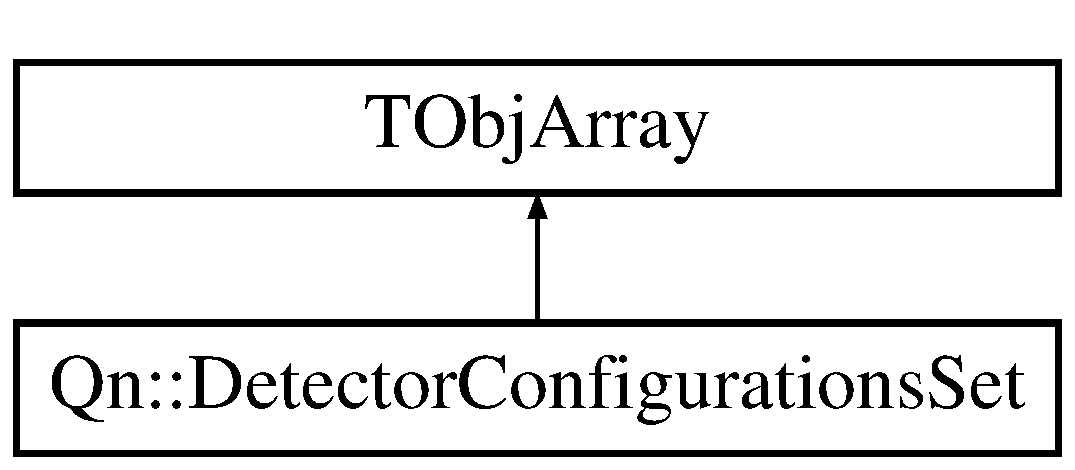
\includegraphics[height=2.000000cm]{classQn_1_1DetectorConfigurationsSet}
\end{center}
\end{figure}
\subsection*{Public Member Functions}
\begin{DoxyCompactItemize}
\item 
\mbox{\Hypertarget{classQn_1_1DetectorConfigurationsSet_a586fc43387363a6c2672369968241b0f}\label{classQn_1_1DetectorConfigurationsSet_a586fc43387363a6c2672369968241b0f}} 
\mbox{\hyperlink{classQn_1_1DetectorConfigurationsSet_a586fc43387363a6c2672369968241b0f}{Detector\+Configurations\+Set}} ()
\begin{DoxyCompactList}\small\item\em Default constructor. \end{DoxyCompactList}\item 
\mbox{\Hypertarget{classQn_1_1DetectorConfigurationsSet_af038bf7441528067a130e68a995ff03d}\label{classQn_1_1DetectorConfigurationsSet_af038bf7441528067a130e68a995ff03d}} 
virtual \mbox{\hyperlink{classQn_1_1DetectorConfigurationsSet_af038bf7441528067a130e68a995ff03d}{$\sim$\+Detector\+Configurations\+Set}} ()
\begin{DoxyCompactList}\small\item\em Default destructor. \end{DoxyCompactList}\item 
virtual \mbox{\hyperlink{classQn_1_1DetectorConfiguration}{Detector\+Configuration}} $\ast$ \mbox{\hyperlink{classQn_1_1DetectorConfigurationsSet_ac9f2135ccb4de759e8d870b5eaeca96a}{At}} (Int\+\_\+t i) const
\end{DoxyCompactItemize}


\subsection{Member Function Documentation}
\mbox{\Hypertarget{classQn_1_1DetectorConfigurationsSet_ac9f2135ccb4de759e8d870b5eaeca96a}\label{classQn_1_1DetectorConfigurationsSet_ac9f2135ccb4de759e8d870b5eaeca96a}} 
\index{Qn\+::\+Detector\+Configurations\+Set@{Qn\+::\+Detector\+Configurations\+Set}!At@{At}}
\index{At@{At}!Qn\+::\+Detector\+Configurations\+Set@{Qn\+::\+Detector\+Configurations\+Set}}
\subsubsection{\texorpdfstring{At()}{At()}}
{\footnotesize\ttfamily virtual \mbox{\hyperlink{classQn_1_1DetectorConfiguration}{Detector\+Configuration}}$\ast$ Qn\+::\+Detector\+Configurations\+Set\+::\+At (\begin{DoxyParamCaption}\item[{Int\+\_\+t}]{i }\end{DoxyParamCaption}) const\hspace{0.3cm}{\ttfamily [inline]}, {\ttfamily [virtual]}}

Access the detector configuration at the passed position 
\begin{DoxyParams}{Parameters}
{\em i} & position in the list (starting at zero) \\
\hline
\end{DoxyParams}
\begin{DoxyReturn}{Returns}
the detector configuration object a position i 
\end{DoxyReturn}


The documentation for this class was generated from the following files\+:\begin{DoxyCompactItemize}
\item 
D\+T\+\_\+\+Flow/\+Qn\+Corrections/include/Detector\+Configurations\+Set.\+h\item 
D\+T\+\_\+\+Flow/\+Qn\+Corrections/Correction\+Detector\+Configurations\+Set.\+cpp\end{DoxyCompactItemize}

\hypertarget{classQn_1_1DetectorConfigurationTracks}{}\section{Qn\+:\+:Detector\+Configuration\+Tracks Class Reference}
\label{classQn_1_1DetectorConfigurationTracks}\index{Qn\+::\+Detector\+Configuration\+Tracks@{Qn\+::\+Detector\+Configuration\+Tracks}}
Inheritance diagram for Qn\+:\+:Detector\+Configuration\+Tracks\+:\begin{figure}[H]
\begin{center}
\leavevmode
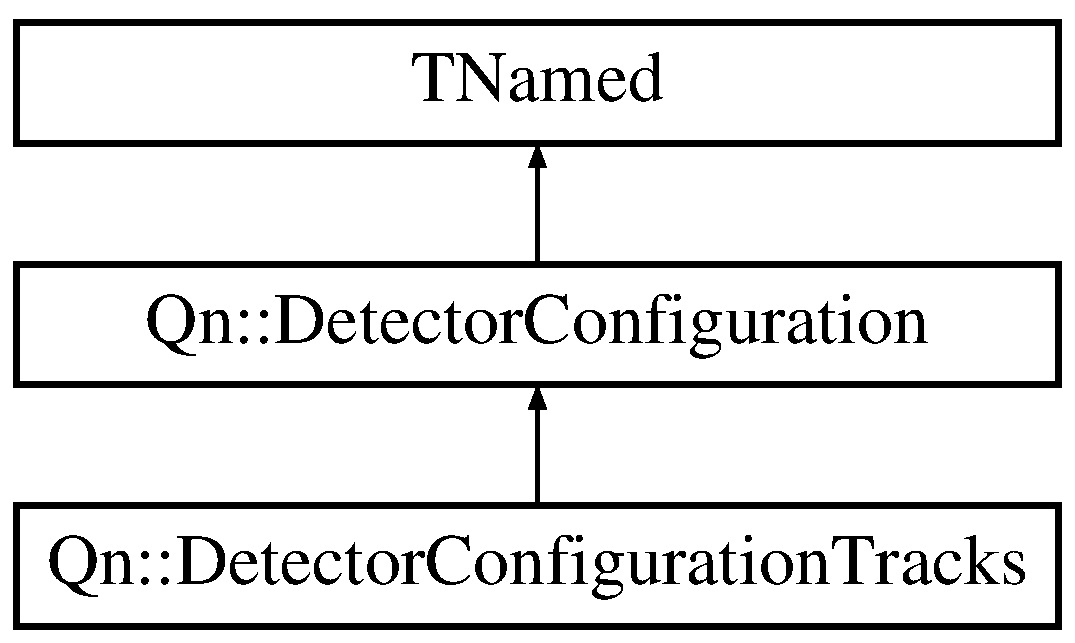
\includegraphics[height=3.000000cm]{classQn_1_1DetectorConfigurationTracks}
\end{center}
\end{figure}
\subsection*{Public Member Functions}
\begin{DoxyCompactItemize}
\item 
\mbox{\Hypertarget{classQn_1_1DetectorConfigurationTracks_a5db99a138323b8eb767560a9a5b6534b}\label{classQn_1_1DetectorConfigurationTracks_a5db99a138323b8eb767560a9a5b6534b}} 
\mbox{\hyperlink{classQn_1_1DetectorConfigurationTracks_a5db99a138323b8eb767560a9a5b6534b}{Detector\+Configuration\+Tracks}} ()
\begin{DoxyCompactList}\small\item\em Default constructor. \end{DoxyCompactList}\item 
\mbox{\hyperlink{classQn_1_1DetectorConfigurationTracks_aa98f7415c841d953a1c8b78d874c19d5}{Detector\+Configuration\+Tracks}} (const char $\ast$name, \mbox{\hyperlink{classQn_1_1EventClassVariablesSet}{Event\+Class\+Variables\+Set}} $\ast$event\+Classes\+Variables, Int\+\_\+t n\+No\+Of\+Harmonics, Int\+\_\+t $\ast$harmonic\+Map=N\+U\+LL)
\item 
virtual \mbox{\hyperlink{classQn_1_1DetectorConfigurationTracks_a60ea7cb759b7170b7447ed2e1b506d27}{$\sim$\+Detector\+Configuration\+Tracks}} ()
\item 
virtual Bool\+\_\+t \mbox{\hyperlink{classQn_1_1DetectorConfigurationTracks_ac9b06051e9ec37086f071308e5031b62}{Get\+Is\+Tracking\+Detector}} () const
\item 
virtual void \mbox{\hyperlink{classQn_1_1DetectorConfigurationTracks_a555a9d8add7610402173b755b77bf57d}{Attach\+Corrections\+Manager}} (\mbox{\hyperlink{classQn_1_1CorrectionCalculator}{Correction\+Calculator}} $\ast$manager)
\item 
virtual void \mbox{\hyperlink{classQn_1_1DetectorConfigurationTracks_aef11ff21d7c3fe4b612fe7c886023c7a}{Create\+Support\+Data\+Structures}} ()
\item 
virtual Bool\+\_\+t \mbox{\hyperlink{classQn_1_1DetectorConfigurationTracks_ab32b2790ce27053d640e2682dcc9223d}{Create\+Support\+Histograms}} (T\+List $\ast$list)
\item 
virtual Bool\+\_\+t \mbox{\hyperlink{classQn_1_1DetectorConfigurationTracks_a4ccffb90904f7769abc11c09f5217337}{Create\+Q\+A\+Histograms}} (T\+List $\ast$list)
\item 
virtual Bool\+\_\+t \mbox{\hyperlink{classQn_1_1DetectorConfigurationTracks_a34818d88b49d67ae71561ffd71c02ec1}{Create\+Nve\+Q\+A\+Histograms}} (T\+List $\ast$list)
\item 
virtual Bool\+\_\+t \mbox{\hyperlink{classQn_1_1DetectorConfigurationTracks_afd9a049e63b16797cd03e6b54d8e209e}{Attach\+Correction\+Inputs}} (T\+List $\ast$list)
\item 
virtual void \mbox{\hyperlink{classQn_1_1DetectorConfigurationTracks_af7f3db92b08c789136fdc0ab97e6576e}{After\+Inputs\+Attach\+Actions}} ()
\item 
virtual Bool\+\_\+t \mbox{\hyperlink{classQn_1_1DetectorConfigurationTracks_a14705aef0b98cfe6d2b20c51676bcc0a}{Process\+Corrections}} (const double $\ast$variable\+Container)
\item 
virtual Bool\+\_\+t \mbox{\hyperlink{classQn_1_1DetectorConfigurationTracks_ab47360b36191cf52c8c9227c3f90fc85}{Process\+Data\+Collection}} (const double $\ast$variable\+Container)
\item 
virtual Bool\+\_\+t \mbox{\hyperlink{classQn_1_1DetectorConfigurationTracks_a0bfa5af566c04893c1c673ddcae7a7c5}{Add\+Data\+Vector}} (const double $\ast$variable\+Container, Double\+\_\+t phi, Double\+\_\+t weight=1.\+0, Int\+\_\+t channel\+Id=-\/1)
\item 
virtual void \mbox{\hyperlink{classQn_1_1DetectorConfigurationTracks_a9194c0e1f6e84a8c8fc249b05ee8afb5}{Build\+Qn\+Vector}} ()
\item 
virtual void \mbox{\hyperlink{classQn_1_1DetectorConfigurationTracks_ac1c478bdcd744a466d0665eb6062317f}{Include\+Qn\+Vectors}} (T\+List $\ast$list)
\item 
virtual void \mbox{\hyperlink{classQn_1_1DetectorConfigurationTracks_a3ef9f093c8d272b48f7371b23eb3d498}{Fill\+Overall\+Input\+Correction\+Step\+List}} (T\+List $\ast$list) const
\item 
virtual void \mbox{\hyperlink{classQn_1_1DetectorConfigurationTracks_a4e725e8d949ab829c804b4e5d9323ff6}{Fill\+Overall\+Qn\+Vector\+Correction\+Step\+List}} (T\+List $\ast$list) const
\item 
virtual void \mbox{\hyperlink{classQn_1_1DetectorConfigurationTracks_a7f28703d7e981a3a0c2fe89116194087}{Report\+On\+Corrections}} (T\+List $\ast$steps, T\+List $\ast$calib, T\+List $\ast$apply) const
\item 
virtual Bool\+\_\+t \mbox{\hyperlink{classQn_1_1DetectorConfigurationTracks_a5382a901ca706cab5df207b3c503df65}{Is\+Selected}} (const double $\ast$variable\+Container)
\item 
\mbox{\Hypertarget{classQn_1_1DetectorConfigurationTracks_a0f65ed87a9163d30aa8897dec30c4b8d}\label{classQn_1_1DetectorConfigurationTracks_a0f65ed87a9163d30aa8897dec30c4b8d}} 
virtual Bool\+\_\+t \mbox{\hyperlink{classQn_1_1DetectorConfigurationTracks_a0f65ed87a9163d30aa8897dec30c4b8d}{Is\+Selected}} (const double $\ast$variable\+Container, Int\+\_\+t n\+Channel)
\begin{DoxyCompactList}\small\item\em wrong call for this class invoke base class behavior \end{DoxyCompactList}\item 
virtual void \mbox{\hyperlink{classQn_1_1DetectorConfigurationTracks_aba7ffa70d60483d7e51460e4309b0fb2}{Clear\+Configuration}} ()
\end{DoxyCompactItemize}
\subsection*{Friends}
\begin{DoxyCompactItemize}
\item 
\mbox{\Hypertarget{classQn_1_1DetectorConfigurationTracks_afbb351f0a159c2e61159977b03f4b3c1}\label{classQn_1_1DetectorConfigurationTracks_afbb351f0a159c2e61159977b03f4b3c1}} 
class {\bfseries Correction\+Step\+Base}
\item 
\mbox{\Hypertarget{classQn_1_1DetectorConfigurationTracks_aaaec1af05216df7a0fa18215ef18023b}\label{classQn_1_1DetectorConfigurationTracks_aaaec1af05216df7a0fa18215ef18023b}} 
class {\bfseries Correction\+Detector}
\end{DoxyCompactItemize}
\subsection*{Additional Inherited Members}


\subsection{Constructor \& Destructor Documentation}
\mbox{\Hypertarget{classQn_1_1DetectorConfigurationTracks_aa98f7415c841d953a1c8b78d874c19d5}\label{classQn_1_1DetectorConfigurationTracks_aa98f7415c841d953a1c8b78d874c19d5}} 
\index{Qn\+::\+Detector\+Configuration\+Tracks@{Qn\+::\+Detector\+Configuration\+Tracks}!Detector\+Configuration\+Tracks@{Detector\+Configuration\+Tracks}}
\index{Detector\+Configuration\+Tracks@{Detector\+Configuration\+Tracks}!Qn\+::\+Detector\+Configuration\+Tracks@{Qn\+::\+Detector\+Configuration\+Tracks}}
\subsubsection{\texorpdfstring{Detector\+Configuration\+Tracks()}{DetectorConfigurationTracks()}}
{\footnotesize\ttfamily Qn\+::\+Detector\+Configuration\+Tracks\+::\+Detector\+Configuration\+Tracks (\begin{DoxyParamCaption}\item[{const char $\ast$}]{name,  }\item[{\mbox{\hyperlink{classQn_1_1EventClassVariablesSet}{Event\+Class\+Variables\+Set}} $\ast$}]{event\+Classes\+Variables,  }\item[{Int\+\_\+t}]{n\+No\+Of\+Harmonics,  }\item[{Int\+\_\+t $\ast$}]{harmonic\+Map = {\ttfamily NULL} }\end{DoxyParamCaption})}

Normal constructor Allocates the data vector bank. 
\begin{DoxyParams}{Parameters}
{\em name} & the name of the detector configuration \\
\hline
{\em event\+Classes\+Variables} & the set of event classes variables \\
\hline
{\em n\+No\+Of\+Harmonics} & the number of harmonics that must be handled \\
\hline
{\em harmonic\+Map} & an optional ordered array with the harmonic numbers \\
\hline
\end{DoxyParams}
\mbox{\Hypertarget{classQn_1_1DetectorConfigurationTracks_a60ea7cb759b7170b7447ed2e1b506d27}\label{classQn_1_1DetectorConfigurationTracks_a60ea7cb759b7170b7447ed2e1b506d27}} 
\index{Qn\+::\+Detector\+Configuration\+Tracks@{Qn\+::\+Detector\+Configuration\+Tracks}!````~Detector\+Configuration\+Tracks@{$\sim$\+Detector\+Configuration\+Tracks}}
\index{````~Detector\+Configuration\+Tracks@{$\sim$\+Detector\+Configuration\+Tracks}!Qn\+::\+Detector\+Configuration\+Tracks@{Qn\+::\+Detector\+Configuration\+Tracks}}
\subsubsection{\texorpdfstring{$\sim$\+Detector\+Configuration\+Tracks()}{~DetectorConfigurationTracks()}}
{\footnotesize\ttfamily Qn\+::\+Detector\+Configuration\+Tracks\+::$\sim$\+Detector\+Configuration\+Tracks (\begin{DoxyParamCaption}{ }\end{DoxyParamCaption})\hspace{0.3cm}{\ttfamily [virtual]}}

Default destructor Memory taken is released by the parent class destructor 

\subsection{Member Function Documentation}
\mbox{\Hypertarget{classQn_1_1DetectorConfigurationTracks_a0bfa5af566c04893c1c673ddcae7a7c5}\label{classQn_1_1DetectorConfigurationTracks_a0bfa5af566c04893c1c673ddcae7a7c5}} 
\index{Qn\+::\+Detector\+Configuration\+Tracks@{Qn\+::\+Detector\+Configuration\+Tracks}!Add\+Data\+Vector@{Add\+Data\+Vector}}
\index{Add\+Data\+Vector@{Add\+Data\+Vector}!Qn\+::\+Detector\+Configuration\+Tracks@{Qn\+::\+Detector\+Configuration\+Tracks}}
\subsubsection{\texorpdfstring{Add\+Data\+Vector()}{AddDataVector()}}
{\footnotesize\ttfamily Bool\+\_\+t Qn\+::\+Detector\+Configuration\+Tracks\+::\+Add\+Data\+Vector (\begin{DoxyParamCaption}\item[{const double $\ast$}]{variable\+Container,  }\item[{Double\+\_\+t}]{phi,  }\item[{Double\+\_\+t}]{weight = {\ttfamily 1.0},  }\item[{Int\+\_\+t}]{id = {\ttfamily -\/1} }\end{DoxyParamCaption})\hspace{0.3cm}{\ttfamily [inline]}, {\ttfamily [virtual]}}

New data vector for the detector configuration. A check is made to see if the current variable bank content passes the associated cuts. If so, the data vector is stored. 
\begin{DoxyParams}{Parameters}
{\em variable\+Container} & pointer to the variable content bank \\
\hline
{\em phi} & azimuthal angle \\
\hline
{\em weight} & the weight associated to the data vector. For track detector is usually one. \\
\hline
{\em id} & the Id associated to the data vector. For track detector configurations could represent the track id. \\
\hline
\end{DoxyParams}
\begin{DoxyReturn}{Returns}
k\+T\+R\+UE if the data vector was accepted and stored 
\end{DoxyReturn}
add the data vector to the bank 

Implements \mbox{\hyperlink{classQn_1_1DetectorConfiguration_ab406e0d2a85e7f5a7c74d0bd0252375d}{Qn\+::\+Detector\+Configuration}}.

\mbox{\Hypertarget{classQn_1_1DetectorConfigurationTracks_af7f3db92b08c789136fdc0ab97e6576e}\label{classQn_1_1DetectorConfigurationTracks_af7f3db92b08c789136fdc0ab97e6576e}} 
\index{Qn\+::\+Detector\+Configuration\+Tracks@{Qn\+::\+Detector\+Configuration\+Tracks}!After\+Inputs\+Attach\+Actions@{After\+Inputs\+Attach\+Actions}}
\index{After\+Inputs\+Attach\+Actions@{After\+Inputs\+Attach\+Actions}!Qn\+::\+Detector\+Configuration\+Tracks@{Qn\+::\+Detector\+Configuration\+Tracks}}
\subsubsection{\texorpdfstring{After\+Inputs\+Attach\+Actions()}{AfterInputsAttachActions()}}
{\footnotesize\ttfamily void Qn\+::\+Detector\+Configuration\+Tracks\+::\+After\+Inputs\+Attach\+Actions (\begin{DoxyParamCaption}{ }\end{DoxyParamCaption})\hspace{0.3cm}{\ttfamily [virtual]}}

Perform after calibration histograms attach actions It is used to inform the different correction step that all conditions for running the network are in place so it is time to check if their requirements are satisfied

The request is transmitted to the Q vector corrections 

Implements \mbox{\hyperlink{classQn_1_1DetectorConfiguration_ab6766905dffe5811aefa59dd1e1117d8}{Qn\+::\+Detector\+Configuration}}.

\mbox{\Hypertarget{classQn_1_1DetectorConfigurationTracks_afd9a049e63b16797cd03e6b54d8e209e}\label{classQn_1_1DetectorConfigurationTracks_afd9a049e63b16797cd03e6b54d8e209e}} 
\index{Qn\+::\+Detector\+Configuration\+Tracks@{Qn\+::\+Detector\+Configuration\+Tracks}!Attach\+Correction\+Inputs@{Attach\+Correction\+Inputs}}
\index{Attach\+Correction\+Inputs@{Attach\+Correction\+Inputs}!Qn\+::\+Detector\+Configuration\+Tracks@{Qn\+::\+Detector\+Configuration\+Tracks}}
\subsubsection{\texorpdfstring{Attach\+Correction\+Inputs()}{AttachCorrectionInputs()}}
{\footnotesize\ttfamily Bool\+\_\+t Qn\+::\+Detector\+Configuration\+Tracks\+::\+Attach\+Correction\+Inputs (\begin{DoxyParamCaption}\item[{T\+List $\ast$}]{list }\end{DoxyParamCaption})\hspace{0.3cm}{\ttfamily [virtual]}}

Asks for attaching the needed input information to the correction steps

The detector list is extracted from the passed list and then the request is transmitted to the Q vector corrections with the found list. 
\begin{DoxyParams}{Parameters}
{\em list} & list where the input information should be found \\
\hline
\end{DoxyParams}
\begin{DoxyReturn}{Returns}
k\+T\+R\+UE if everything went OK 
\end{DoxyReturn}


Implements \mbox{\hyperlink{classQn_1_1DetectorConfiguration_a4ae0eb587070e68a11fbb438d96fca15}{Qn\+::\+Detector\+Configuration}}.

\mbox{\Hypertarget{classQn_1_1DetectorConfigurationTracks_a555a9d8add7610402173b755b77bf57d}\label{classQn_1_1DetectorConfigurationTracks_a555a9d8add7610402173b755b77bf57d}} 
\index{Qn\+::\+Detector\+Configuration\+Tracks@{Qn\+::\+Detector\+Configuration\+Tracks}!Attach\+Corrections\+Manager@{Attach\+Corrections\+Manager}}
\index{Attach\+Corrections\+Manager@{Attach\+Corrections\+Manager}!Qn\+::\+Detector\+Configuration\+Tracks@{Qn\+::\+Detector\+Configuration\+Tracks}}
\subsubsection{\texorpdfstring{Attach\+Corrections\+Manager()}{AttachCorrectionsManager()}}
{\footnotesize\ttfamily void Qn\+::\+Detector\+Configuration\+Tracks\+::\+Attach\+Corrections\+Manager (\begin{DoxyParamCaption}\item[{\mbox{\hyperlink{classQn_1_1CorrectionCalculator}{Correction\+Calculator}} $\ast$}]{manager }\end{DoxyParamCaption})\hspace{0.3cm}{\ttfamily [virtual]}}

Stores the framework manager pointer Orders the base class to store the correction manager and informs the \mbox{\hyperlink{namespaceQn}{Qn}} vector corrections they are now attached to the framework 
\begin{DoxyParams}{Parameters}
{\em manager} & the framework manager \\
\hline
\end{DoxyParams}


Implements \mbox{\hyperlink{classQn_1_1DetectorConfiguration_a512c77d73e0e6453607f7ae7e2e8f72b}{Qn\+::\+Detector\+Configuration}}.

\mbox{\Hypertarget{classQn_1_1DetectorConfigurationTracks_a9194c0e1f6e84a8c8fc249b05ee8afb5}\label{classQn_1_1DetectorConfigurationTracks_a9194c0e1f6e84a8c8fc249b05ee8afb5}} 
\index{Qn\+::\+Detector\+Configuration\+Tracks@{Qn\+::\+Detector\+Configuration\+Tracks}!Build\+Qn\+Vector@{Build\+Qn\+Vector}}
\index{Build\+Qn\+Vector@{Build\+Qn\+Vector}!Qn\+::\+Detector\+Configuration\+Tracks@{Qn\+::\+Detector\+Configuration\+Tracks}}
\subsubsection{\texorpdfstring{Build\+Qn\+Vector()}{BuildQnVector()}}
{\footnotesize\ttfamily void Qn\+::\+Detector\+Configuration\+Tracks\+::\+Build\+Qn\+Vector (\begin{DoxyParamCaption}{ }\end{DoxyParamCaption})\hspace{0.3cm}{\ttfamily [inline]}, {\ttfamily [virtual]}}

Builds \mbox{\hyperlink{namespaceQn}{Qn}} vectors before Q vector corrections but considering the chosen calibration method. Remember, this configuration does not have a channelized approach so, the built Q vectors are the ones to be used for subsequent corrections. 

Implements \mbox{\hyperlink{classQn_1_1DetectorConfiguration_a7aaf10f6e30151dd142d59d5dff72e2d}{Qn\+::\+Detector\+Configuration}}.

\mbox{\Hypertarget{classQn_1_1DetectorConfigurationTracks_aba7ffa70d60483d7e51460e4309b0fb2}\label{classQn_1_1DetectorConfigurationTracks_aba7ffa70d60483d7e51460e4309b0fb2}} 
\index{Qn\+::\+Detector\+Configuration\+Tracks@{Qn\+::\+Detector\+Configuration\+Tracks}!Clear\+Configuration@{Clear\+Configuration}}
\index{Clear\+Configuration@{Clear\+Configuration}!Qn\+::\+Detector\+Configuration\+Tracks@{Qn\+::\+Detector\+Configuration\+Tracks}}
\subsubsection{\texorpdfstring{Clear\+Configuration()}{ClearConfiguration()}}
{\footnotesize\ttfamily void Qn\+::\+Detector\+Configuration\+Tracks\+::\+Clear\+Configuration (\begin{DoxyParamCaption}{ }\end{DoxyParamCaption})\hspace{0.3cm}{\ttfamily [inline]}, {\ttfamily [virtual]}}

Clean the configuration to accept a new event

Transfers the order to the Q vector correction steps and cleans the own Q vector and the input data vector bank for accepting the next event. 

Implements \mbox{\hyperlink{classQn_1_1DetectorConfiguration_a94c21b39a4a3680675319aacf4a517f4}{Qn\+::\+Detector\+Configuration}}.

\mbox{\Hypertarget{classQn_1_1DetectorConfigurationTracks_a34818d88b49d67ae71561ffd71c02ec1}\label{classQn_1_1DetectorConfigurationTracks_a34818d88b49d67ae71561ffd71c02ec1}} 
\index{Qn\+::\+Detector\+Configuration\+Tracks@{Qn\+::\+Detector\+Configuration\+Tracks}!Create\+Nve\+Q\+A\+Histograms@{Create\+Nve\+Q\+A\+Histograms}}
\index{Create\+Nve\+Q\+A\+Histograms@{Create\+Nve\+Q\+A\+Histograms}!Qn\+::\+Detector\+Configuration\+Tracks@{Qn\+::\+Detector\+Configuration\+Tracks}}
\subsubsection{\texorpdfstring{Create\+Nve\+Q\+A\+Histograms()}{CreateNveQAHistograms()}}
{\footnotesize\ttfamily Bool\+\_\+t Qn\+::\+Detector\+Configuration\+Tracks\+::\+Create\+Nve\+Q\+A\+Histograms (\begin{DoxyParamCaption}\item[{T\+List $\ast$}]{list }\end{DoxyParamCaption})\hspace{0.3cm}{\ttfamily [virtual]}}

Asks for non validated entries QA histograms creation

The request is transmitted to the Q vector corrections.

A new histograms list is created for the detector and incorporated to the passed list. Then the new list is passed to the corrections. 
\begin{DoxyParams}{Parameters}
{\em list} & list where the histograms should be incorporated for its persistence \\
\hline
\end{DoxyParams}
\begin{DoxyReturn}{Returns}
k\+T\+R\+UE if everything went OK 
\end{DoxyReturn}


Implements \mbox{\hyperlink{classQn_1_1DetectorConfiguration_ade61875d8e7a05dd413c94d6887ae4ac}{Qn\+::\+Detector\+Configuration}}.

\mbox{\Hypertarget{classQn_1_1DetectorConfigurationTracks_a4ccffb90904f7769abc11c09f5217337}\label{classQn_1_1DetectorConfigurationTracks_a4ccffb90904f7769abc11c09f5217337}} 
\index{Qn\+::\+Detector\+Configuration\+Tracks@{Qn\+::\+Detector\+Configuration\+Tracks}!Create\+Q\+A\+Histograms@{Create\+Q\+A\+Histograms}}
\index{Create\+Q\+A\+Histograms@{Create\+Q\+A\+Histograms}!Qn\+::\+Detector\+Configuration\+Tracks@{Qn\+::\+Detector\+Configuration\+Tracks}}
\subsubsection{\texorpdfstring{Create\+Q\+A\+Histograms()}{CreateQAHistograms()}}
{\footnotesize\ttfamily Bool\+\_\+t Qn\+::\+Detector\+Configuration\+Tracks\+::\+Create\+Q\+A\+Histograms (\begin{DoxyParamCaption}\item[{T\+List $\ast$}]{list }\end{DoxyParamCaption})\hspace{0.3cm}{\ttfamily [virtual]}}

Asks for QA histograms creation

The request is transmitted to the Q vector corrections.

A new histograms list is created for the detector and incorporated to the passed list. Then the new list is passed to the corrections. 
\begin{DoxyParams}{Parameters}
{\em list} & list where the histograms should be incorporated for its persistence \\
\hline
\end{DoxyParams}
\begin{DoxyReturn}{Returns}
k\+T\+R\+UE if everything went OK 
\end{DoxyReturn}


Implements \mbox{\hyperlink{classQn_1_1DetectorConfiguration_a9f527d4c584e6bd79b6b8eb0b7f5413a}{Qn\+::\+Detector\+Configuration}}.

\mbox{\Hypertarget{classQn_1_1DetectorConfigurationTracks_aef11ff21d7c3fe4b612fe7c886023c7a}\label{classQn_1_1DetectorConfigurationTracks_aef11ff21d7c3fe4b612fe7c886023c7a}} 
\index{Qn\+::\+Detector\+Configuration\+Tracks@{Qn\+::\+Detector\+Configuration\+Tracks}!Create\+Support\+Data\+Structures@{Create\+Support\+Data\+Structures}}
\index{Create\+Support\+Data\+Structures@{Create\+Support\+Data\+Structures}!Qn\+::\+Detector\+Configuration\+Tracks@{Qn\+::\+Detector\+Configuration\+Tracks}}
\subsubsection{\texorpdfstring{Create\+Support\+Data\+Structures()}{CreateSupportDataStructures()}}
{\footnotesize\ttfamily void Qn\+::\+Detector\+Configuration\+Tracks\+::\+Create\+Support\+Data\+Structures (\begin{DoxyParamCaption}{ }\end{DoxyParamCaption})\hspace{0.3cm}{\ttfamily [virtual]}}

Asks for support data structures creation

The input data vector bank is allocated and the request is transmitted to the Q vector corrections. 

Implements \mbox{\hyperlink{classQn_1_1DetectorConfiguration_a664f65925f22f8f02c1a216f77b533ce}{Qn\+::\+Detector\+Configuration}}.

\mbox{\Hypertarget{classQn_1_1DetectorConfigurationTracks_ab32b2790ce27053d640e2682dcc9223d}\label{classQn_1_1DetectorConfigurationTracks_ab32b2790ce27053d640e2682dcc9223d}} 
\index{Qn\+::\+Detector\+Configuration\+Tracks@{Qn\+::\+Detector\+Configuration\+Tracks}!Create\+Support\+Histograms@{Create\+Support\+Histograms}}
\index{Create\+Support\+Histograms@{Create\+Support\+Histograms}!Qn\+::\+Detector\+Configuration\+Tracks@{Qn\+::\+Detector\+Configuration\+Tracks}}
\subsubsection{\texorpdfstring{Create\+Support\+Histograms()}{CreateSupportHistograms()}}
{\footnotesize\ttfamily Bool\+\_\+t Qn\+::\+Detector\+Configuration\+Tracks\+::\+Create\+Support\+Histograms (\begin{DoxyParamCaption}\item[{T\+List $\ast$}]{list }\end{DoxyParamCaption})\hspace{0.3cm}{\ttfamily [virtual]}}

Asks for support histograms creation

The request is transmitted to the Q vector corrections.

A new histograms list is created for the detector configuration and incorporated to the passed list. Then the new list is passed to the corrections. 
\begin{DoxyParams}{Parameters}
{\em list} & list where the histograms should be incorporated for its persistence \\
\hline
\end{DoxyParams}
\begin{DoxyReturn}{Returns}
k\+T\+R\+UE if everything went OK 
\end{DoxyReturn}


Implements \mbox{\hyperlink{classQn_1_1DetectorConfiguration_a8e5e2eef94bca58a3dcf34fe5fbd1429}{Qn\+::\+Detector\+Configuration}}.

\mbox{\Hypertarget{classQn_1_1DetectorConfigurationTracks_a3ef9f093c8d272b48f7371b23eb3d498}\label{classQn_1_1DetectorConfigurationTracks_a3ef9f093c8d272b48f7371b23eb3d498}} 
\index{Qn\+::\+Detector\+Configuration\+Tracks@{Qn\+::\+Detector\+Configuration\+Tracks}!Fill\+Overall\+Input\+Correction\+Step\+List@{Fill\+Overall\+Input\+Correction\+Step\+List}}
\index{Fill\+Overall\+Input\+Correction\+Step\+List@{Fill\+Overall\+Input\+Correction\+Step\+List}!Qn\+::\+Detector\+Configuration\+Tracks@{Qn\+::\+Detector\+Configuration\+Tracks}}
\subsubsection{\texorpdfstring{Fill\+Overall\+Input\+Correction\+Step\+List()}{FillOverallInputCorrectionStepList()}}
{\footnotesize\ttfamily void Qn\+::\+Detector\+Configuration\+Tracks\+::\+Fill\+Overall\+Input\+Correction\+Step\+List (\begin{DoxyParamCaption}\item[{T\+List $\ast$}]{list }\end{DoxyParamCaption}) const\hspace{0.3cm}{\ttfamily [virtual]}}

Include only one instance of each input correction step in execution order

There are not input correction so we do nothing 
\begin{DoxyParams}{Parameters}
{\em list} & list where the correction steps should be incorporated \\
\hline
\end{DoxyParams}


Implements \mbox{\hyperlink{classQn_1_1DetectorConfiguration_a76e173f938b886b5575597d9464698b4}{Qn\+::\+Detector\+Configuration}}.

\mbox{\Hypertarget{classQn_1_1DetectorConfigurationTracks_a4e725e8d949ab829c804b4e5d9323ff6}\label{classQn_1_1DetectorConfigurationTracks_a4e725e8d949ab829c804b4e5d9323ff6}} 
\index{Qn\+::\+Detector\+Configuration\+Tracks@{Qn\+::\+Detector\+Configuration\+Tracks}!Fill\+Overall\+Qn\+Vector\+Correction\+Step\+List@{Fill\+Overall\+Qn\+Vector\+Correction\+Step\+List}}
\index{Fill\+Overall\+Qn\+Vector\+Correction\+Step\+List@{Fill\+Overall\+Qn\+Vector\+Correction\+Step\+List}!Qn\+::\+Detector\+Configuration\+Tracks@{Qn\+::\+Detector\+Configuration\+Tracks}}
\subsubsection{\texorpdfstring{Fill\+Overall\+Qn\+Vector\+Correction\+Step\+List()}{FillOverallQnVectorCorrectionStepList()}}
{\footnotesize\ttfamily void Qn\+::\+Detector\+Configuration\+Tracks\+::\+Fill\+Overall\+Qn\+Vector\+Correction\+Step\+List (\begin{DoxyParamCaption}\item[{T\+List $\ast$}]{list }\end{DoxyParamCaption}) const\hspace{0.3cm}{\ttfamily [virtual]}}

Include only one instance of each \mbox{\hyperlink{namespaceQn}{Qn}} vector correction step in execution order

The request is transmitted to the set of \mbox{\hyperlink{namespaceQn}{Qn}} vector corrections 
\begin{DoxyParams}{Parameters}
{\em list} & list where the correction steps should be incorporated \\
\hline
\end{DoxyParams}


Implements \mbox{\hyperlink{classQn_1_1DetectorConfiguration_ad71d83a2b0a5cee45bde15e936843e49}{Qn\+::\+Detector\+Configuration}}.

\mbox{\Hypertarget{classQn_1_1DetectorConfigurationTracks_ac9b06051e9ec37086f071308e5031b62}\label{classQn_1_1DetectorConfigurationTracks_ac9b06051e9ec37086f071308e5031b62}} 
\index{Qn\+::\+Detector\+Configuration\+Tracks@{Qn\+::\+Detector\+Configuration\+Tracks}!Get\+Is\+Tracking\+Detector@{Get\+Is\+Tracking\+Detector}}
\index{Get\+Is\+Tracking\+Detector@{Get\+Is\+Tracking\+Detector}!Qn\+::\+Detector\+Configuration\+Tracks@{Qn\+::\+Detector\+Configuration\+Tracks}}
\subsubsection{\texorpdfstring{Get\+Is\+Tracking\+Detector()}{GetIsTrackingDetector()}}
{\footnotesize\ttfamily virtual Bool\+\_\+t Qn\+::\+Detector\+Configuration\+Tracks\+::\+Get\+Is\+Tracking\+Detector (\begin{DoxyParamCaption}{ }\end{DoxyParamCaption}) const\hspace{0.3cm}{\ttfamily [inline]}, {\ttfamily [virtual]}}

Get if the detector configuration is own by a tracking detector \begin{DoxyReturn}{Returns}
T\+R\+UE, this is tracking detector configuration 
\end{DoxyReturn}


Implements \mbox{\hyperlink{classQn_1_1DetectorConfiguration_acdb57db96ed24524b5a3a28821727a3d}{Qn\+::\+Detector\+Configuration}}.

\mbox{\Hypertarget{classQn_1_1DetectorConfigurationTracks_ac1c478bdcd744a466d0665eb6062317f}\label{classQn_1_1DetectorConfigurationTracks_ac1c478bdcd744a466d0665eb6062317f}} 
\index{Qn\+::\+Detector\+Configuration\+Tracks@{Qn\+::\+Detector\+Configuration\+Tracks}!Include\+Qn\+Vectors@{Include\+Qn\+Vectors}}
\index{Include\+Qn\+Vectors@{Include\+Qn\+Vectors}!Qn\+::\+Detector\+Configuration\+Tracks@{Qn\+::\+Detector\+Configuration\+Tracks}}
\subsubsection{\texorpdfstring{Include\+Qn\+Vectors()}{IncludeQnVectors()}}
{\footnotesize\ttfamily void Qn\+::\+Detector\+Configuration\+Tracks\+::\+Include\+Qn\+Vectors (\begin{DoxyParamCaption}\item[{T\+List $\ast$}]{list }\end{DoxyParamCaption})\hspace{0.3cm}{\ttfamily [virtual]}}

Include the the list of \mbox{\hyperlink{namespaceQn}{Qn}} vector associated to the detector configuration into the passed list

A new list is created for the detector configuration and incorporated to the passed list.

Always includes first the fully corrected \mbox{\hyperlink{namespaceQn}{Qn}} vector, and then includes the plain \mbox{\hyperlink{namespaceQn}{Qn}} vector and asks to the different correction steps to include their partially corrected \mbox{\hyperlink{namespaceQn}{Qn}} vectors. The check if we are already there is because it could be late information about the process name and then the correction histograms could still not be attached and the constructed list does not contain the final \mbox{\hyperlink{namespaceQn}{Qn}} vectors. 
\begin{DoxyParams}{Parameters}
{\em list} & list where the corrected \mbox{\hyperlink{namespaceQn}{Qn}} vector should be added \\
\hline
\end{DoxyParams}


Implements \mbox{\hyperlink{classQn_1_1DetectorConfiguration_a4298530954cc8dabbd41b1fd83d6310f}{Qn\+::\+Detector\+Configuration}}.

\mbox{\Hypertarget{classQn_1_1DetectorConfigurationTracks_a5382a901ca706cab5df207b3c503df65}\label{classQn_1_1DetectorConfigurationTracks_a5382a901ca706cab5df207b3c503df65}} 
\index{Qn\+::\+Detector\+Configuration\+Tracks@{Qn\+::\+Detector\+Configuration\+Tracks}!Is\+Selected@{Is\+Selected}}
\index{Is\+Selected@{Is\+Selected}!Qn\+::\+Detector\+Configuration\+Tracks@{Qn\+::\+Detector\+Configuration\+Tracks}}
\subsubsection{\texorpdfstring{Is\+Selected()}{IsSelected()}}
{\footnotesize\ttfamily virtual Bool\+\_\+t Qn\+::\+Detector\+Configuration\+Tracks\+::\+Is\+Selected (\begin{DoxyParamCaption}\item[{const double $\ast$}]{variable\+Container }\end{DoxyParamCaption})\hspace{0.3cm}{\ttfamily [inline]}, {\ttfamily [virtual]}}

Checks if the current content of the variable bank applies to the detector configuration 
\begin{DoxyParams}{Parameters}
{\em variable\+Container} & pointer to the variable content bank \\
\hline
\end{DoxyParams}
\begin{DoxyReturn}{Returns}
k\+T\+R\+UE if the current content applies to the configuration 
\end{DoxyReturn}


Implements \mbox{\hyperlink{classQn_1_1DetectorConfiguration}{Qn\+::\+Detector\+Configuration}}.

\mbox{\Hypertarget{classQn_1_1DetectorConfigurationTracks_a14705aef0b98cfe6d2b20c51676bcc0a}\label{classQn_1_1DetectorConfigurationTracks_a14705aef0b98cfe6d2b20c51676bcc0a}} 
\index{Qn\+::\+Detector\+Configuration\+Tracks@{Qn\+::\+Detector\+Configuration\+Tracks}!Process\+Corrections@{Process\+Corrections}}
\index{Process\+Corrections@{Process\+Corrections}!Qn\+::\+Detector\+Configuration\+Tracks@{Qn\+::\+Detector\+Configuration\+Tracks}}
\subsubsection{\texorpdfstring{Process\+Corrections()}{ProcessCorrections()}}
{\footnotesize\ttfamily Bool\+\_\+t Qn\+::\+Detector\+Configuration\+Tracks\+::\+Process\+Corrections (\begin{DoxyParamCaption}\item[{const double $\ast$}]{variable\+Container }\end{DoxyParamCaption})\hspace{0.3cm}{\ttfamily [inline]}, {\ttfamily [virtual]}}

Ask for processing corrections for the involved detector configuration

The request is transmitted to the Q vector correction steps. The first not applied correction step breaks the loop and k\+F\+A\+L\+SE is returned \begin{DoxyReturn}{Returns}
k\+T\+R\+UE if all correction steps were applied 
\end{DoxyReturn}


Implements \mbox{\hyperlink{classQn_1_1DetectorConfiguration_aad0610bd5d168c29a32025ddf641e3fc}{Qn\+::\+Detector\+Configuration}}.

\mbox{\Hypertarget{classQn_1_1DetectorConfigurationTracks_ab47360b36191cf52c8c9227c3f90fc85}\label{classQn_1_1DetectorConfigurationTracks_ab47360b36191cf52c8c9227c3f90fc85}} 
\index{Qn\+::\+Detector\+Configuration\+Tracks@{Qn\+::\+Detector\+Configuration\+Tracks}!Process\+Data\+Collection@{Process\+Data\+Collection}}
\index{Process\+Data\+Collection@{Process\+Data\+Collection}!Qn\+::\+Detector\+Configuration\+Tracks@{Qn\+::\+Detector\+Configuration\+Tracks}}
\subsubsection{\texorpdfstring{Process\+Data\+Collection()}{ProcessDataCollection()}}
{\footnotesize\ttfamily Bool\+\_\+t Qn\+::\+Detector\+Configuration\+Tracks\+::\+Process\+Data\+Collection (\begin{DoxyParamCaption}\item[{const double $\ast$}]{variable\+Container }\end{DoxyParamCaption})\hspace{0.3cm}{\ttfamily [inline]}, {\ttfamily [virtual]}}

Ask for processing corrections data collection for the involved detector configuration Fill own QA histogram information and then the request is transmitted to the Q vector correction steps. The first not applied correction step breaks the loop and k\+F\+A\+L\+SE is returned \begin{DoxyReturn}{Returns}
k\+T\+R\+UE if all correction steps were applied 
\end{DoxyReturn}


Implements \mbox{\hyperlink{classQn_1_1DetectorConfiguration_ac78ed44b460217fda7d094cc102504c4}{Qn\+::\+Detector\+Configuration}}.

\mbox{\Hypertarget{classQn_1_1DetectorConfigurationTracks_a7f28703d7e981a3a0c2fe89116194087}\label{classQn_1_1DetectorConfigurationTracks_a7f28703d7e981a3a0c2fe89116194087}} 
\index{Qn\+::\+Detector\+Configuration\+Tracks@{Qn\+::\+Detector\+Configuration\+Tracks}!Report\+On\+Corrections@{Report\+On\+Corrections}}
\index{Report\+On\+Corrections@{Report\+On\+Corrections}!Qn\+::\+Detector\+Configuration\+Tracks@{Qn\+::\+Detector\+Configuration\+Tracks}}
\subsubsection{\texorpdfstring{Report\+On\+Corrections()}{ReportOnCorrections()}}
{\footnotesize\ttfamily void Qn\+::\+Detector\+Configuration\+Tracks\+::\+Report\+On\+Corrections (\begin{DoxyParamCaption}\item[{T\+List $\ast$}]{steps,  }\item[{T\+List $\ast$}]{calib,  }\item[{T\+List $\ast$}]{apply }\end{DoxyParamCaption}) const\hspace{0.3cm}{\ttfamily [virtual]}}

Provide information about assigned corrections

We create three list which items they own, incorporate info from the correction steps and add them to the passed list 
\begin{DoxyParams}{Parameters}
{\em steps} & list for incorporating the list of assigned correction steps \\
\hline
{\em calib} & list for incorporating the list of steps in calibrating status \\
\hline
{\em apply} & list for incorporating the list of steps in applying status \\
\hline
\end{DoxyParams}


Implements \mbox{\hyperlink{classQn_1_1DetectorConfiguration_ad33e54cbf374fa37d8edf9915719982f}{Qn\+::\+Detector\+Configuration}}.



The documentation for this class was generated from the following files\+:\begin{DoxyCompactItemize}
\item 
D\+T\+\_\+\+Flow/\+Qn\+Corrections/include/Detector\+Configuration\+Tracks.\+h\item 
D\+T\+\_\+\+Flow/\+Qn\+Corrections/Detector\+Configuration\+Tracks.\+cpp\end{DoxyCompactItemize}

\hypertarget{classQn_1_1Efficiency}{}\section{Qn\+:\+:Efficiency Class Reference}
\label{classQn_1_1Efficiency}\index{Qn\+::\+Efficiency@{Qn\+::\+Efficiency}}
\subsection*{Public Types}
\begin{DoxyCompactItemize}
\item 
\mbox{\Hypertarget{classQn_1_1Efficiency_af2846ec080a0960b2247f929da405cbb}\label{classQn_1_1Efficiency_af2846ec080a0960b2247f929da405cbb}} 
enum {\bfseries Passed} \+: bool \{ {\bfseries Yes} = true, 
{\bfseries No} = false
 \}
\end{DoxyCompactItemize}
\subsection*{Public Member Functions}
\begin{DoxyCompactItemize}
\item 
\mbox{\Hypertarget{classQn_1_1Efficiency_a03f2282ff7e4352d8f7a4500f0f82008}\label{classQn_1_1Efficiency_a03f2282ff7e4352d8f7a4500f0f82008}} 
void {\bfseries Update} (Efficiency\+::\+Passed pass)
\item 
\mbox{\Hypertarget{classQn_1_1Efficiency_ae0e3e892fcf788469f1b3ed39e78f7f2}\label{classQn_1_1Efficiency_ae0e3e892fcf788469f1b3ed39e78f7f2}} 
float {\bfseries Get\+Efficiency} ()
\item 
\mbox{\Hypertarget{classQn_1_1Efficiency_ab4273c19749d748d601220cf8750897d}\label{classQn_1_1Efficiency_ab4273c19749d748d601220cf8750897d}} 
float {\bfseries Get\+Error\+Up} ()
\item 
\mbox{\Hypertarget{classQn_1_1Efficiency_a13ef74fcbd052fa99fb558676b2e6880}\label{classQn_1_1Efficiency_a13ef74fcbd052fa99fb558676b2e6880}} 
float {\bfseries Get\+Error\+Low} ()
\end{DoxyCompactItemize}


The documentation for this class was generated from the following file\+:\begin{DoxyCompactItemize}
\item 
D\+T\+\_\+\+Flow/\+Base/include/Efficiency.\+h\end{DoxyCompactItemize}

\hypertarget{classQn_1_1EseHandler}{}\section{Qn\+:\+:Ese\+Handler Class Reference}
\label{classQn_1_1EseHandler}\index{Qn\+::\+Ese\+Handler@{Qn\+::\+Ese\+Handler}}
\subsection*{Public Member Functions}
\begin{DoxyCompactItemize}
\item 
\mbox{\Hypertarget{classQn_1_1EseHandler_a850d2ba21ed46c6b58db070f8aeebcdd}\label{classQn_1_1EseHandler_a850d2ba21ed46c6b58db070f8aeebcdd}} 
{\bfseries Ese\+Handler} (\mbox{\hyperlink{classQn_1_1CorrelationManager}{Correlation\+Manager}} $\ast$man)
\item 
void \mbox{\hyperlink{classQn_1_1EseHandler_abf21f1c9e2e1a2c27d6b1ab47ec68129}{Set\+Input}} (std\+::string percentiles\+\_\+name, std\+::string calib\+\_\+filename)
\item 
\mbox{\Hypertarget{classQn_1_1EseHandler_af0841190bbabe156205c60fcc71f9ce8}\label{classQn_1_1EseHandler_af0841190bbabe156205c60fcc71f9ce8}} 
void {\bfseries Set\+Output} (const std\+::string \&tree\+\_\+filename, const std\+::string \&calib\+\_\+filename)
\item 
\mbox{\Hypertarget{classQn_1_1EseHandler_a3c711e44aac8fb825f1d4ef4d3b0516a}\label{classQn_1_1EseHandler_a3c711e44aac8fb825f1d4ef4d3b0516a}} 
void {\bfseries Add\+E\+SE} (const std\+::string \&name, const std\+::vector$<$ std\+::string $>$ \&input, Correlation\+::function\+\_\+t lambda, const T\+H1F \&histo)
\item 
\mbox{\Hypertarget{classQn_1_1EseHandler_a77b88da6beb8cc6bd09ad532f67ec6bd}\label{classQn_1_1EseHandler_a77b88da6beb8cc6bd09ad532f67ec6bd}} 
void {\bfseries Connect} ()
\item 
\mbox{\Hypertarget{classQn_1_1EseHandler_a185d3735cf4528256d19f840c67dde33}\label{classQn_1_1EseHandler_a185d3735cf4528256d19f840c67dde33}} 
void {\bfseries Initialize} ()
\item 
\mbox{\Hypertarget{classQn_1_1EseHandler_ae03099ea62473d19fecbc93e952f14d8}\label{classQn_1_1EseHandler_ae03099ea62473d19fecbc93e952f14d8}} 
void {\bfseries Configure} ()
\item 
\mbox{\Hypertarget{classQn_1_1EseHandler_a02e572f6df586a2f222d8a1060d06670}\label{classQn_1_1EseHandler_a02e572f6df586a2f222d8a1060d06670}} 
bool {\bfseries Process} (const std\+::vector$<$ unsigned long $>$ \&eventindices)
\item 
\mbox{\Hypertarget{classQn_1_1EseHandler_ab21cb6361b59abdd561c8d699b306c0e}\label{classQn_1_1EseHandler_ab21cb6361b59abdd561c8d699b306c0e}} 
void {\bfseries Finalize} ()
\item 
\mbox{\Hypertarget{classQn_1_1EseHandler_ac2fadcf9fe900fa85bf45e7baba0c7b6}\label{classQn_1_1EseHandler_ac2fadcf9fe900fa85bf45e7baba0c7b6}} 
std\+::string {\bfseries Report} ()
\item 
\mbox{\Hypertarget{classQn_1_1EseHandler_a439a4135d422cf6ff02ed423fc6d3027}\label{classQn_1_1EseHandler_a439a4135d422cf6ff02ed423fc6d3027}} 
\mbox{\hyperlink{classQn_1_1Correlation}{Qn\+::\+Correlation}} $\ast$ {\bfseries Request\+Correlation} (const \mbox{\hyperlink{structQn_1_1SubEventPrototype}{Sub\+Event\+Prototype}} \&prototype)
\item 
\mbox{\Hypertarget{classQn_1_1EseHandler_a873146ccc642528b792f6ac37a01d8ff}\label{classQn_1_1EseHandler_a873146ccc642528b792f6ac37a01d8ff}} 
void {\bfseries Request\+Event\+Axis} (const \mbox{\hyperlink{classQn_1_1Axis}{Qn\+::\+Axis}} \&axis)
\item 
\mbox{\Hypertarget{classQn_1_1EseHandler_aac107400e625db5e486916fc319c5c6a}\label{classQn_1_1EseHandler_aac107400e625db5e486916fc319c5c6a}} 
void {\bfseries Fill\+Tree} ()
\item 
\mbox{\Hypertarget{classQn_1_1EseHandler_a254210229fd9fee761db873cbc4ecb95}\label{classQn_1_1EseHandler_a254210229fd9fee761db873cbc4ecb95}} 
void {\bfseries Set\+Run\+Event\+Id} (const std\+::string \&run, const std\+::string \&event)
\item 
\mbox{\Hypertarget{classQn_1_1EseHandler_a27ac3d056224ad8860498ecb5ac28cbc}\label{classQn_1_1EseHandler_a27ac3d056224ad8860498ecb5ac28cbc}} 
void {\bfseries Setup\+Event\+Matching} ()
\item 
\mbox{\Hypertarget{classQn_1_1EseHandler_a6c36a5bf30214de0ba6c075d559dcf22}\label{classQn_1_1EseHandler_a6c36a5bf30214de0ba6c075d559dcf22}} 
bool {\bfseries Check\+Matching} ()
\item 
\mbox{\Hypertarget{classQn_1_1EseHandler_a158f5b4c4e3b590adea0d4bbfbb8a708}\label{classQn_1_1EseHandler_a158f5b4c4e3b590adea0d4bbfbb8a708}} 
void {\bfseries Update\+I\+Ds} ()
\end{DoxyCompactItemize}


\subsection{Member Function Documentation}
\mbox{\Hypertarget{classQn_1_1EseHandler_abf21f1c9e2e1a2c27d6b1ab47ec68129}\label{classQn_1_1EseHandler_abf21f1c9e2e1a2c27d6b1ab47ec68129}} 
\index{Qn\+::\+Ese\+Handler@{Qn\+::\+Ese\+Handler}!Set\+Input@{Set\+Input}}
\index{Set\+Input@{Set\+Input}!Qn\+::\+Ese\+Handler@{Qn\+::\+Ese\+Handler}}
\subsubsection{\texorpdfstring{Set\+Input()}{SetInput()}}
{\footnotesize\ttfamily void Qn\+::\+Ese\+Handler\+::\+Set\+Input (\begin{DoxyParamCaption}\item[{std\+::string}]{percentiles\+\_\+name,  }\item[{std\+::string}]{calib\+\_\+filename }\end{DoxyParamCaption})}

Sets inputs. Root file is read when it is found in the path. 
\begin{DoxyParams}{Parameters}
{\em percentiles\+\_\+name} & full path of the input percentiles tree. \\
\hline
{\em calib\+\_\+filename} & full path of the calibration file. \\
\hline
\end{DoxyParams}


The documentation for this class was generated from the following files\+:\begin{DoxyCompactItemize}
\item 
D\+T\+\_\+\+Flow/\+Correlation/include/Ese\+Handler.\+h\item 
D\+T\+\_\+\+Flow/\+Correlation/Ese\+Handler.\+cpp\end{DoxyCompactItemize}

\hypertarget{classQn_1_1EseSubEvent}{}\section{Qn\+:\+:Ese\+Sub\+Event Class Reference}
\label{classQn_1_1EseSubEvent}\index{Qn\+::\+Ese\+Sub\+Event@{Qn\+::\+Ese\+Sub\+Event}}
\subsection*{Public Types}
\begin{DoxyCompactItemize}
\item 
\mbox{\Hypertarget{classQn_1_1EseSubEvent_a2687faacf0aaaacd1a80bbc51614aa07}\label{classQn_1_1EseSubEvent_a2687faacf0aaaacd1a80bbc51614aa07}} 
enum {\bfseries State} \+: int \{ {\bfseries unini} = 0, 
{\bfseries collect} = 1, 
{\bfseries calib} = 2, 
{\bfseries percent} = 3
 \}
\end{DoxyCompactItemize}
\subsection*{Public Member Functions}
\begin{DoxyCompactItemize}
\item 
\mbox{\Hypertarget{classQn_1_1EseSubEvent_ac89c06299684f76e6b8110074a42d553}\label{classQn_1_1EseSubEvent_ac89c06299684f76e6b8110074a42d553}} 
{\bfseries Ese\+Sub\+Event} (\mbox{\hyperlink{classQn_1_1EseHandler}{Ese\+Handler}} $\ast$handler, const std\+::string \&name, const std\+::vector$<$ std\+::string $>$ \&input, Correlation\+::function\+\_\+t lambda, const T\+H1F \&histo)
\item 
\mbox{\Hypertarget{classQn_1_1EseSubEvent_a8243c90d1d7aa2fc6e0308cb18bf4569}\label{classQn_1_1EseSubEvent_a8243c90d1d7aa2fc6e0308cb18bf4569}} 
void {\bfseries Connect\+Input} (T\+File $\ast$input\+\_\+treefile, T\+File $\ast$calib)
\item 
\mbox{\Hypertarget{classQn_1_1EseSubEvent_aaac0a65949ae1c1dfdf29d7e4987267f}\label{classQn_1_1EseSubEvent_aaac0a65949ae1c1dfdf29d7e4987267f}} 
void {\bfseries Connect\+Output} (T\+Tree $\ast$tree, T\+File $\ast$calib)
\item 
\mbox{\Hypertarget{classQn_1_1EseSubEvent_a6bc3388985fc0715ba32e378d428834c}\label{classQn_1_1EseSubEvent_a6bc3388985fc0715ba32e378d428834c}} 
void {\bfseries Configure} ()
\item 
\mbox{\Hypertarget{classQn_1_1EseSubEvent_adb6e9050cf7cfa775ad07affb94b4ab8}\label{classQn_1_1EseSubEvent_adb6e9050cf7cfa775ad07affb94b4ab8}} 
void {\bfseries Add\+Correlation} ()
\item 
\mbox{\Hypertarget{classQn_1_1EseSubEvent_ab67dbd34169aeb9880ae68819bc21bb2}\label{classQn_1_1EseSubEvent_ab67dbd34169aeb9880ae68819bc21bb2}} 
void {\bfseries Do} (const std\+::vector$<$ unsigned long $>$ \&eventindices)
\item 
\mbox{\Hypertarget{classQn_1_1EseSubEvent_a0748197895abc2934bd441642983c750}\label{classQn_1_1EseSubEvent_a0748197895abc2934bd441642983c750}} 
void {\bfseries Clear} ()
\item 
\mbox{\Hypertarget{classQn_1_1EseSubEvent_a2fc8b53006e70b3afb4669a5a98a5c5a}\label{classQn_1_1EseSubEvent_a2fc8b53006e70b3afb4669a5a98a5c5a}} 
void {\bfseries Finalize} ()
\item 
\mbox{\Hypertarget{classQn_1_1EseSubEvent_a0b3b24e583618bebf4d364edcfc8cc55}\label{classQn_1_1EseSubEvent_a0b3b24e583618bebf4d364edcfc8cc55}} 
std\+::string {\bfseries Report} ()
\item 
\mbox{\Hypertarget{classQn_1_1EseSubEvent_a810c864e00edeeaad1b3c8abc6a86092}\label{classQn_1_1EseSubEvent_a810c864e00edeeaad1b3c8abc6a86092}} 
State {\bfseries Get\+State} () const
\end{DoxyCompactItemize}
\subsection*{Static Public Attributes}
\begin{DoxyCompactItemize}
\item 
\mbox{\Hypertarget{classQn_1_1EseSubEvent_a98a8b4d32230d9e80900f33b07a5d0ff}\label{classQn_1_1EseSubEvent_a98a8b4d32230d9e80900f33b07a5d0ff}} 
static constexpr int {\bfseries k\+N\+Bins} = 10
\end{DoxyCompactItemize}


The documentation for this class was generated from the following files\+:\begin{DoxyCompactItemize}
\item 
D\+T\+\_\+\+Flow/\+Correlation/include/Ese\+Sub\+Event.\+h\item 
D\+T\+\_\+\+Flow/\+Correlation/Ese\+Sub\+Event.\+cpp\end{DoxyCompactItemize}

\hypertarget{classQn_1_1EventAxes}{}\section{Qn\+:\+:Event\+Axes Class Reference}
\label{classQn_1_1EventAxes}\index{Qn\+::\+Event\+Axes@{Qn\+::\+Event\+Axes}}


{\ttfamily \#include $<$Event\+Axes.\+h$>$}

\subsection*{Public Types}
\begin{DoxyCompactItemize}
\item 
enum \mbox{\hyperlink{classQn_1_1EventAxes_a81ebc6649920a462e33c176287b8706c}{Type}} \{ {\bfseries Integer}, 
{\bfseries Float}
 \}
\end{DoxyCompactItemize}
\subsection*{Public Member Functions}
\begin{DoxyCompactItemize}
\item 
\mbox{\Hypertarget{classQn_1_1EventAxes_aaafb27e11f7e5feb8aebff6f18703f84}\label{classQn_1_1EventAxes_aaafb27e11f7e5feb8aebff6f18703f84}} 
{\bfseries Event\+Axes} (\mbox{\hyperlink{classQn_1_1CorrelationManager}{Qn\+::\+Correlation\+Manager}} $\ast$manager)
\item 
void \mbox{\hyperlink{classQn_1_1EventAxes_a4ddaaed5f02c92e5fa6696be9bf397e9}{Register\+Event\+Axis}} (\mbox{\hyperlink{classQn_1_1Axis}{Axis}} axis, \mbox{\hyperlink{classQn_1_1EventAxes_a81ebc6649920a462e33c176287b8706c}{Type}} type)
\begin{DoxyCompactList}\small\item\em Registers a new axes with a specific datatype to be read from the tree and used for binning. \end{DoxyCompactList}\item 
bool \mbox{\hyperlink{classQn_1_1EventAxes_a979183927f0ded4af0b1b22385550c2a}{Check\+Event}} ()
\begin{DoxyCompactList}\small\item\em Check if current event is inside the event axes. \end{DoxyCompactList}\item 
const std\+::vector$<$ \mbox{\hyperlink{classQn_1_1Axis}{Qn\+::\+Axis}} $>$ \mbox{\hyperlink{classQn_1_1EventAxes_a784b89dd78c0fe3a0fe6c57ef0835c23}{Get\+Axes}} () const
\begin{DoxyCompactList}\small\item\em Returns a vector of the event axes. \end{DoxyCompactList}\item 
const std\+::vector$<$ unsigned long $>$ \& \mbox{\hyperlink{classQn_1_1EventAxes_a76d3881ef0c333be3044c6b0b706e7e7}{Get\+Bin}} () const
\begin{DoxyCompactList}\small\item\em Returns the current event bin. \end{DoxyCompactList}\end{DoxyCompactItemize}


\subsection{Detailed Description}
A collection of \mbox{\hyperlink{classQn_1_1EventAxis}{Event\+Axis}} with methods to facilitate the binning of event variables. 

\subsection{Member Enumeration Documentation}
\mbox{\Hypertarget{classQn_1_1EventAxes_a81ebc6649920a462e33c176287b8706c}\label{classQn_1_1EventAxes_a81ebc6649920a462e33c176287b8706c}} 
\index{Qn\+::\+Event\+Axes@{Qn\+::\+Event\+Axes}!Type@{Type}}
\index{Type@{Type}!Qn\+::\+Event\+Axes@{Qn\+::\+Event\+Axes}}
\subsubsection{\texorpdfstring{Type}{Type}}
{\footnotesize\ttfamily enum \mbox{\hyperlink{classQn_1_1EventAxes_a81ebc6649920a462e33c176287b8706c}{Qn\+::\+Event\+Axes\+::\+Type}}\hspace{0.3cm}{\ttfamily [strong]}}

Enumerator to specify the underlying data type in the input tree. 

\subsection{Member Function Documentation}
\mbox{\Hypertarget{classQn_1_1EventAxes_a979183927f0ded4af0b1b22385550c2a}\label{classQn_1_1EventAxes_a979183927f0ded4af0b1b22385550c2a}} 
\index{Qn\+::\+Event\+Axes@{Qn\+::\+Event\+Axes}!Check\+Event@{Check\+Event}}
\index{Check\+Event@{Check\+Event}!Qn\+::\+Event\+Axes@{Qn\+::\+Event\+Axes}}
\subsubsection{\texorpdfstring{Check\+Event()}{CheckEvent()}}
{\footnotesize\ttfamily bool Qn\+::\+Event\+Axes\+::\+Check\+Event (\begin{DoxyParamCaption}{ }\end{DoxyParamCaption})\hspace{0.3cm}{\ttfamily [inline]}}



Check if current event is inside the event axes. 

\begin{DoxyReturn}{Returns}
Returns true if the event is inside the event axes. 
\end{DoxyReturn}
\mbox{\Hypertarget{classQn_1_1EventAxes_a784b89dd78c0fe3a0fe6c57ef0835c23}\label{classQn_1_1EventAxes_a784b89dd78c0fe3a0fe6c57ef0835c23}} 
\index{Qn\+::\+Event\+Axes@{Qn\+::\+Event\+Axes}!Get\+Axes@{Get\+Axes}}
\index{Get\+Axes@{Get\+Axes}!Qn\+::\+Event\+Axes@{Qn\+::\+Event\+Axes}}
\subsubsection{\texorpdfstring{Get\+Axes()}{GetAxes()}}
{\footnotesize\ttfamily const std\+::vector$<$\mbox{\hyperlink{classQn_1_1Axis}{Qn\+::\+Axis}}$>$ Qn\+::\+Event\+Axes\+::\+Get\+Axes (\begin{DoxyParamCaption}{ }\end{DoxyParamCaption}) const\hspace{0.3cm}{\ttfamily [inline]}}



Returns a vector of the event axes. 

\begin{DoxyReturn}{Returns}
vector of axes 
\end{DoxyReturn}
\mbox{\Hypertarget{classQn_1_1EventAxes_a76d3881ef0c333be3044c6b0b706e7e7}\label{classQn_1_1EventAxes_a76d3881ef0c333be3044c6b0b706e7e7}} 
\index{Qn\+::\+Event\+Axes@{Qn\+::\+Event\+Axes}!Get\+Bin@{Get\+Bin}}
\index{Get\+Bin@{Get\+Bin}!Qn\+::\+Event\+Axes@{Qn\+::\+Event\+Axes}}
\subsubsection{\texorpdfstring{Get\+Bin()}{GetBin()}}
{\footnotesize\ttfamily const std\+::vector$<$unsigned long$>$\& Qn\+::\+Event\+Axes\+::\+Get\+Bin (\begin{DoxyParamCaption}{ }\end{DoxyParamCaption}) const\hspace{0.3cm}{\ttfamily [inline]}}



Returns the current event bin. 

\begin{DoxyReturn}{Returns}
multidimensional bin 
\end{DoxyReturn}
\mbox{\Hypertarget{classQn_1_1EventAxes_a4ddaaed5f02c92e5fa6696be9bf397e9}\label{classQn_1_1EventAxes_a4ddaaed5f02c92e5fa6696be9bf397e9}} 
\index{Qn\+::\+Event\+Axes@{Qn\+::\+Event\+Axes}!Register\+Event\+Axis@{Register\+Event\+Axis}}
\index{Register\+Event\+Axis@{Register\+Event\+Axis}!Qn\+::\+Event\+Axes@{Qn\+::\+Event\+Axes}}
\subsubsection{\texorpdfstring{Register\+Event\+Axis()}{RegisterEventAxis()}}
{\footnotesize\ttfamily void Qn\+::\+Event\+Axes\+::\+Register\+Event\+Axis (\begin{DoxyParamCaption}\item[{\mbox{\hyperlink{classQn_1_1Axis}{Qn\+::\+Axis}}}]{axis,  }\item[{\mbox{\hyperlink{classQn_1_1EventAxes_a81ebc6649920a462e33c176287b8706c}{Type}}}]{type }\end{DoxyParamCaption})}



Registers a new axes with a specific datatype to be read from the tree and used for binning. 


\begin{DoxyParams}{Parameters}
{\em axis} & \mbox{\hyperlink{classQn_1_1Axis}{Axis}} specifing the name and the size of the binning for the correlations. \\
\hline
{\em type} & Data type in which the information was saved to the tree. \\
\hline
\end{DoxyParams}


The documentation for this class was generated from the following files\+:\begin{DoxyCompactItemize}
\item 
D\+T\+\_\+\+Flow/\+Correlation/include/Event\+Axes.\+h\item 
D\+T\+\_\+\+Flow/\+Correlation/Event\+Axes.\+cpp\end{DoxyCompactItemize}

\hypertarget{classQn_1_1EventAxis}{}\section{Qn\+:\+:Event\+Axis$<$ T $>$ Class Template Reference}
\label{classQn_1_1EventAxis}\index{Qn\+::\+Event\+Axis$<$ T $>$@{Qn\+::\+Event\+Axis$<$ T $>$}}


{\ttfamily \#include $<$Event\+Axes.\+h$>$}

Inheritance diagram for Qn\+:\+:Event\+Axis$<$ T $>$\+:\begin{figure}[H]
\begin{center}
\leavevmode
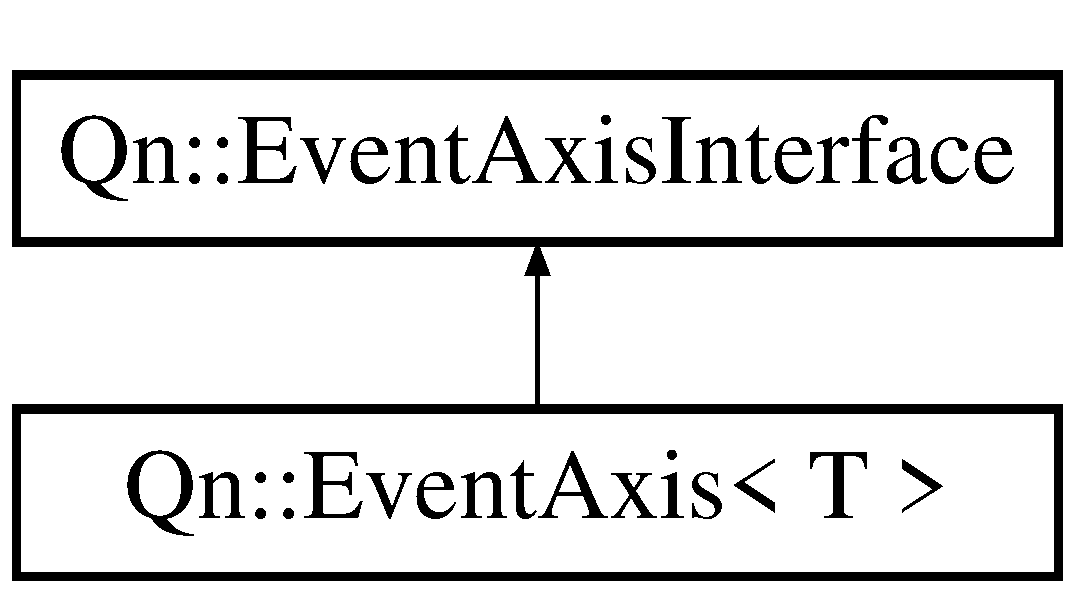
\includegraphics[height=2.000000cm]{classQn_1_1EventAxis}
\end{center}
\end{figure}
\subsection*{Public Member Functions}
\begin{DoxyCompactItemize}
\item 
\mbox{\hyperlink{classQn_1_1EventAxis_a801e914dd851f39aeab25b048d95a039}{Event\+Axis}} (const \mbox{\hyperlink{classQn_1_1Axis}{Qn\+::\+Axis}} \&axis, T\+Tree\+Reader\+Value$<$ T $>$ value)
\begin{DoxyCompactList}\small\item\em Constructor. \end{DoxyCompactList}\item 
unsigned long \mbox{\hyperlink{classQn_1_1EventAxis_af5799b86d0e326c4d7b2e31e4a6ba086}{Get\+Bin}} () override
\begin{DoxyCompactList}\small\item\em Get the current event bin. Information of the variable is read directly from the tree. \end{DoxyCompactList}\item 
const \mbox{\hyperlink{classQn_1_1Axis}{Qn\+::\+Axis}} \& \mbox{\hyperlink{classQn_1_1EventAxis_a7fba5bcfeb2877ced0aa0006ce82d26c}{Get\+Axis}} () const override
\begin{DoxyCompactList}\small\item\em Get the underlying \mbox{\hyperlink{classQn_1_1Axis}{Qn\+::\+Axis}}. \end{DoxyCompactList}\item 
bool \mbox{\hyperlink{classQn_1_1EventAxis_a503c69f641f36b6717ffc167b53abd56}{Is\+Valid}} () override
\end{DoxyCompactItemize}


\subsection{Detailed Description}
\subsubsection*{template$<$typename T$>$\newline
class Qn\+::\+Event\+Axis$<$ T $>$}

Template class for event axes of different underlying data type. 
\begin{DoxyTemplParams}{Template Parameters}
{\em T} & Data type of the variable in the input T\+Tree. \\
\hline
\end{DoxyTemplParams}


\subsection{Constructor \& Destructor Documentation}
\mbox{\Hypertarget{classQn_1_1EventAxis_a801e914dd851f39aeab25b048d95a039}\label{classQn_1_1EventAxis_a801e914dd851f39aeab25b048d95a039}} 
\index{Qn\+::\+Event\+Axis@{Qn\+::\+Event\+Axis}!Event\+Axis@{Event\+Axis}}
\index{Event\+Axis@{Event\+Axis}!Qn\+::\+Event\+Axis@{Qn\+::\+Event\+Axis}}
\subsubsection{\texorpdfstring{Event\+Axis()}{EventAxis()}}
{\footnotesize\ttfamily template$<$typename T $>$ \\
\mbox{\hyperlink{classQn_1_1EventAxis}{Qn\+::\+Event\+Axis}}$<$ T $>$\+::\mbox{\hyperlink{classQn_1_1EventAxis}{Event\+Axis}} (\begin{DoxyParamCaption}\item[{const \mbox{\hyperlink{classQn_1_1Axis}{Qn\+::\+Axis}} \&}]{axis,  }\item[{T\+Tree\+Reader\+Value$<$ T $>$}]{value }\end{DoxyParamCaption})\hspace{0.3cm}{\ttfamily [inline]}}



Constructor. 


\begin{DoxyParams}{Parameters}
{\em axis} & Binning of the \mbox{\hyperlink{classQn_1_1EventAxis}{Event\+Axis}}. \\
\hline
{\em value} & Associated value in the input tree \\
\hline
\end{DoxyParams}


\subsection{Member Function Documentation}
\mbox{\Hypertarget{classQn_1_1EventAxis_a7fba5bcfeb2877ced0aa0006ce82d26c}\label{classQn_1_1EventAxis_a7fba5bcfeb2877ced0aa0006ce82d26c}} 
\index{Qn\+::\+Event\+Axis@{Qn\+::\+Event\+Axis}!Get\+Axis@{Get\+Axis}}
\index{Get\+Axis@{Get\+Axis}!Qn\+::\+Event\+Axis@{Qn\+::\+Event\+Axis}}
\subsubsection{\texorpdfstring{Get\+Axis()}{GetAxis()}}
{\footnotesize\ttfamily template$<$typename T $>$ \\
const \mbox{\hyperlink{classQn_1_1Axis}{Qn\+::\+Axis}}\& \mbox{\hyperlink{classQn_1_1EventAxis}{Qn\+::\+Event\+Axis}}$<$ T $>$\+::Get\+Axis (\begin{DoxyParamCaption}{ }\end{DoxyParamCaption}) const\hspace{0.3cm}{\ttfamily [inline]}, {\ttfamily [override]}, {\ttfamily [virtual]}}



Get the underlying \mbox{\hyperlink{classQn_1_1Axis}{Qn\+::\+Axis}}. 

\begin{DoxyReturn}{Returns}
Returns the underlying \mbox{\hyperlink{classQn_1_1Axis}{Qn\+::\+Axis}} 
\end{DoxyReturn}


Implements \mbox{\hyperlink{classQn_1_1EventAxisInterface}{Qn\+::\+Event\+Axis\+Interface}}.

\mbox{\Hypertarget{classQn_1_1EventAxis_af5799b86d0e326c4d7b2e31e4a6ba086}\label{classQn_1_1EventAxis_af5799b86d0e326c4d7b2e31e4a6ba086}} 
\index{Qn\+::\+Event\+Axis@{Qn\+::\+Event\+Axis}!Get\+Bin@{Get\+Bin}}
\index{Get\+Bin@{Get\+Bin}!Qn\+::\+Event\+Axis@{Qn\+::\+Event\+Axis}}
\subsubsection{\texorpdfstring{Get\+Bin()}{GetBin()}}
{\footnotesize\ttfamily template$<$typename T $>$ \\
unsigned long \mbox{\hyperlink{classQn_1_1EventAxis}{Qn\+::\+Event\+Axis}}$<$ T $>$\+::Get\+Bin (\begin{DoxyParamCaption}{ }\end{DoxyParamCaption})\hspace{0.3cm}{\ttfamily [inline]}, {\ttfamily [override]}, {\ttfamily [virtual]}}



Get the current event bin. Information of the variable is read directly from the tree. 

\begin{DoxyReturn}{Returns}
bin to which the current value belongs to. 
\end{DoxyReturn}


Implements \mbox{\hyperlink{classQn_1_1EventAxisInterface}{Qn\+::\+Event\+Axis\+Interface}}.

\mbox{\Hypertarget{classQn_1_1EventAxis_a503c69f641f36b6717ffc167b53abd56}\label{classQn_1_1EventAxis_a503c69f641f36b6717ffc167b53abd56}} 
\index{Qn\+::\+Event\+Axis@{Qn\+::\+Event\+Axis}!Is\+Valid@{Is\+Valid}}
\index{Is\+Valid@{Is\+Valid}!Qn\+::\+Event\+Axis@{Qn\+::\+Event\+Axis}}
\subsubsection{\texorpdfstring{Is\+Valid()}{IsValid()}}
{\footnotesize\ttfamily template$<$typename T $>$ \\
bool \mbox{\hyperlink{classQn_1_1EventAxis}{Qn\+::\+Event\+Axis}}$<$ T $>$\+::Is\+Valid (\begin{DoxyParamCaption}{ }\end{DoxyParamCaption})\hspace{0.3cm}{\ttfamily [inline]}, {\ttfamily [override]}, {\ttfamily [virtual]}}

Checks if the current entry read from the tree is a valid number (no N\+AN in case of float) \begin{DoxyReturn}{Returns}
Returns true if the current entry is a valid number. 
\end{DoxyReturn}


Implements \mbox{\hyperlink{classQn_1_1EventAxisInterface}{Qn\+::\+Event\+Axis\+Interface}}.



The documentation for this class was generated from the following file\+:\begin{DoxyCompactItemize}
\item 
D\+T\+\_\+\+Flow/\+Correlation/include/Event\+Axes.\+h\end{DoxyCompactItemize}

\hypertarget{classQn_1_1EventAxisInterface}{}\section{Qn\+:\+:Event\+Axis\+Interface Class Reference}
\label{classQn_1_1EventAxisInterface}\index{Qn\+::\+Event\+Axis\+Interface@{Qn\+::\+Event\+Axis\+Interface}}


{\ttfamily \#include $<$Event\+Axes.\+h$>$}

Inheritance diagram for Qn\+:\+:Event\+Axis\+Interface\+:\begin{figure}[H]
\begin{center}
\leavevmode
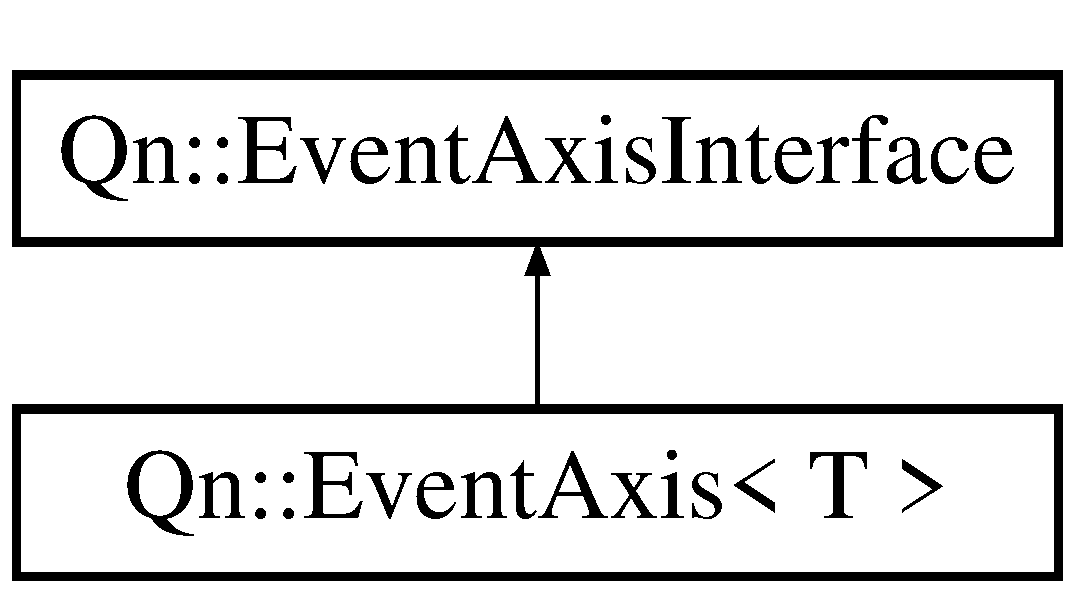
\includegraphics[height=2.000000cm]{classQn_1_1EventAxisInterface}
\end{center}
\end{figure}
\subsection*{Public Member Functions}
\begin{DoxyCompactItemize}
\item 
\mbox{\Hypertarget{classQn_1_1EventAxisInterface_a3676d7d832b7fcad5907a5015f472589}\label{classQn_1_1EventAxisInterface_a3676d7d832b7fcad5907a5015f472589}} 
virtual unsigned long {\bfseries Get\+Bin} ()=0
\item 
\mbox{\Hypertarget{classQn_1_1EventAxisInterface_ab10571521568059db24ed885ca37d336}\label{classQn_1_1EventAxisInterface_ab10571521568059db24ed885ca37d336}} 
virtual bool {\bfseries Is\+Valid} ()=0
\item 
\mbox{\Hypertarget{classQn_1_1EventAxisInterface_aa0e99311e6deb3b2f072faa284bf244e}\label{classQn_1_1EventAxisInterface_aa0e99311e6deb3b2f072faa284bf244e}} 
virtual const \mbox{\hyperlink{classQn_1_1Axis}{Qn\+::\+Axis}} \& {\bfseries Get\+Axis} () const =0
\end{DoxyCompactItemize}


\subsection{Detailed Description}
\mbox{\hyperlink{classBase}{Base}} class of the Event Axes 

The documentation for this class was generated from the following file\+:\begin{DoxyCompactItemize}
\item 
D\+T\+\_\+\+Flow/\+Correlation/include/Event\+Axes.\+h\end{DoxyCompactItemize}

\hypertarget{classQn_1_1EventClassVariable}{}\section{Qn\+:\+:Event\+Class\+Variable Class Reference}
\label{classQn_1_1EventClassVariable}\index{Qn\+::\+Event\+Class\+Variable@{Qn\+::\+Event\+Class\+Variable}}
Inheritance diagram for Qn\+:\+:Event\+Class\+Variable\+:\begin{figure}[H]
\begin{center}
\leavevmode
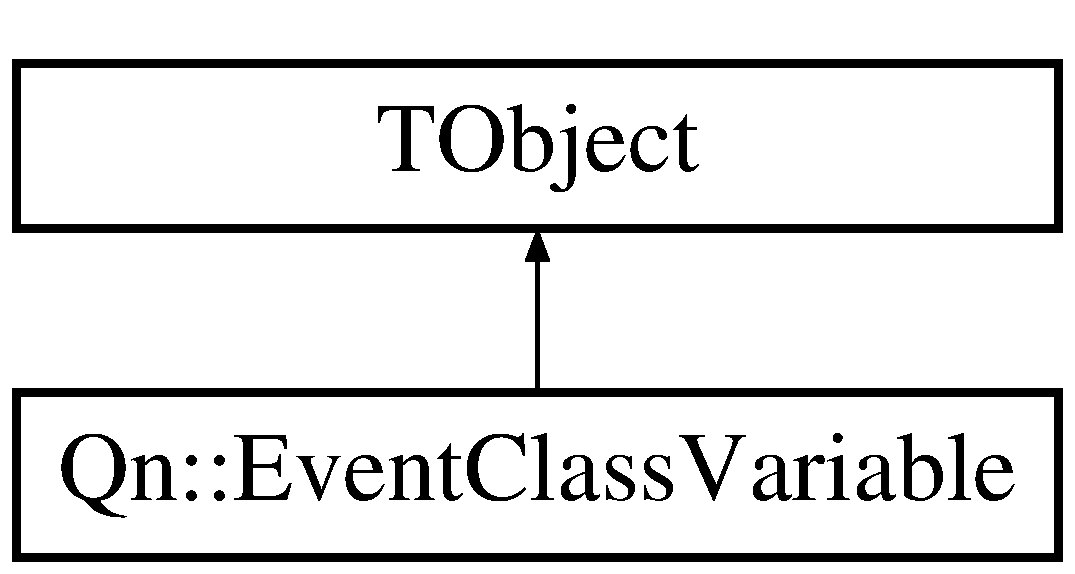
\includegraphics[height=2.000000cm]{classQn_1_1EventClassVariable}
\end{center}
\end{figure}
\subsection*{Public Member Functions}
\begin{DoxyCompactItemize}
\item 
\mbox{\Hypertarget{classQn_1_1EventClassVariable_aa733d204603ec159a936c1e92b2ba7e5}\label{classQn_1_1EventClassVariable_aa733d204603ec159a936c1e92b2ba7e5}} 
\mbox{\hyperlink{classQn_1_1EventClassVariable_aa733d204603ec159a936c1e92b2ba7e5}{Event\+Class\+Variable}} ()
\begin{DoxyCompactList}\small\item\em Default constructor. \end{DoxyCompactList}\item 
\mbox{\Hypertarget{classQn_1_1EventClassVariable_a7b8a5c162d249c21010237a6cd5553ef}\label{classQn_1_1EventClassVariable_a7b8a5c162d249c21010237a6cd5553ef}} 
\mbox{\hyperlink{classQn_1_1EventClassVariable_a7b8a5c162d249c21010237a6cd5553ef}{Event\+Class\+Variable}} (const \mbox{\hyperlink{classQn_1_1EventClassVariable}{Event\+Class\+Variable}} \&ecv)
\begin{DoxyCompactList}\small\item\em Copy constructor. \end{DoxyCompactList}\item 
\mbox{\hyperlink{classQn_1_1EventClassVariable_af1700dd291428bf69331c8ba9d092b7e}{Event\+Class\+Variable}} (Int\+\_\+t var\+Id, const char $\ast$varname, Int\+\_\+t nbins, Double\+\_\+t min, Double\+\_\+t max)
\item 
\mbox{\hyperlink{classQn_1_1EventClassVariable_aadc0846404621e79c573b98e7747039b}{Event\+Class\+Variable}} (Int\+\_\+t var\+Id, const char $\ast$varname, Int\+\_\+t nbins, Double\+\_\+t $\ast$bins)
\item 
\mbox{\hyperlink{classQn_1_1EventClassVariable_a260ffe64770085c450a4666670760931}{Event\+Class\+Variable}} (Int\+\_\+t var\+Id, const char $\ast$varname, Double\+\_\+t bins\+Array\mbox{[}$\,$\mbox{]}\mbox{[}2\mbox{]})
\item 
\mbox{\hyperlink{classQn_1_1EventClassVariable_a8143fbc405d4946f2bfa34fb965f3a0d}{$\sim$\+Event\+Class\+Variable}} ()
\item 
\mbox{\Hypertarget{classQn_1_1EventClassVariable_aff7924928b5c2e6e31bcfd9ddc1c63d1}\label{classQn_1_1EventClassVariable_aff7924928b5c2e6e31bcfd9ddc1c63d1}} 
Int\+\_\+t \mbox{\hyperlink{classQn_1_1EventClassVariable_aff7924928b5c2e6e31bcfd9ddc1c63d1}{Get\+Variable\+Id}} () const
\begin{DoxyCompactList}\small\item\em Gets the variable unique Id. \end{DoxyCompactList}\item 
\mbox{\Hypertarget{classQn_1_1EventClassVariable_a1375e59e436e9f548d73e4f0b088e383}\label{classQn_1_1EventClassVariable_a1375e59e436e9f548d73e4f0b088e383}} 
const char $\ast$ \mbox{\hyperlink{classQn_1_1EventClassVariable_a1375e59e436e9f548d73e4f0b088e383}{Get\+Variable\+Label}} () const
\begin{DoxyCompactList}\small\item\em Gets the variable name / label. \end{DoxyCompactList}\item 
\mbox{\Hypertarget{classQn_1_1EventClassVariable_a1062547d193d6cbee57c372aded6e735}\label{classQn_1_1EventClassVariable_a1062547d193d6cbee57c372aded6e735}} 
Int\+\_\+t \mbox{\hyperlink{classQn_1_1EventClassVariable_a1062547d193d6cbee57c372aded6e735}{Get\+N\+Bins}} () const
\begin{DoxyCompactList}\small\item\em Gets the number of bins. \end{DoxyCompactList}\item 
\mbox{\Hypertarget{classQn_1_1EventClassVariable_a0ccf71156817657ed2a63e6b6c16c2e2}\label{classQn_1_1EventClassVariable_a0ccf71156817657ed2a63e6b6c16c2e2}} 
const Double\+\_\+t $\ast$ \mbox{\hyperlink{classQn_1_1EventClassVariable_a0ccf71156817657ed2a63e6b6c16c2e2}{Get\+Bins}} () const
\begin{DoxyCompactList}\small\item\em Gets the actual bins edges array. \end{DoxyCompactList}\item 
Double\+\_\+t \mbox{\hyperlink{classQn_1_1EventClassVariable_a117fcb0c7496e08d6aa61f24a52cc652}{Get\+Bin\+Lower\+Edge}} (Int\+\_\+t bin) const
\item 
Double\+\_\+t \mbox{\hyperlink{classQn_1_1EventClassVariable_a457a9a46cdfd22f3496da1e113baba3d}{Get\+Bin\+Upper\+Edge}} (Int\+\_\+t bin) const
\item 
\mbox{\Hypertarget{classQn_1_1EventClassVariable_a32e9a9a359d84000ad39623b0914cc2e}\label{classQn_1_1EventClassVariable_a32e9a9a359d84000ad39623b0914cc2e}} 
Double\+\_\+t \mbox{\hyperlink{classQn_1_1EventClassVariable_a32e9a9a359d84000ad39623b0914cc2e}{Get\+Lower\+Edge}} ()
\begin{DoxyCompactList}\small\item\em Gets the lowest variable value considered. \end{DoxyCompactList}\item 
\mbox{\Hypertarget{classQn_1_1EventClassVariable_a6b6eb035ec93b8f42e70b9be3e4f1506}\label{classQn_1_1EventClassVariable_a6b6eb035ec93b8f42e70b9be3e4f1506}} 
Double\+\_\+t \mbox{\hyperlink{classQn_1_1EventClassVariable_a6b6eb035ec93b8f42e70b9be3e4f1506}{Get\+Upper\+Edge}} ()
\begin{DoxyCompactList}\small\item\em Gets the highest variabel value considered. \end{DoxyCompactList}\end{DoxyCompactItemize}


\subsection{Constructor \& Destructor Documentation}
\mbox{\Hypertarget{classQn_1_1EventClassVariable_af1700dd291428bf69331c8ba9d092b7e}\label{classQn_1_1EventClassVariable_af1700dd291428bf69331c8ba9d092b7e}} 
\index{Qn\+::\+Event\+Class\+Variable@{Qn\+::\+Event\+Class\+Variable}!Event\+Class\+Variable@{Event\+Class\+Variable}}
\index{Event\+Class\+Variable@{Event\+Class\+Variable}!Qn\+::\+Event\+Class\+Variable@{Qn\+::\+Event\+Class\+Variable}}
\subsubsection{\texorpdfstring{Event\+Class\+Variable()}{EventClassVariable()}\hspace{0.1cm}{\footnotesize\ttfamily [1/3]}}
{\footnotesize\ttfamily Qn\+::\+Event\+Class\+Variable\+::\+Event\+Class\+Variable (\begin{DoxyParamCaption}\item[{Int\+\_\+t}]{var\+Id,  }\item[{const char $\ast$}]{varname,  }\item[{Int\+\_\+t}]{nbins,  }\item[{Double\+\_\+t}]{min,  }\item[{Double\+\_\+t}]{max }\end{DoxyParamCaption})}

Normal constructor

Allocates memory for the desired number of bins (plus one) and build their lower and upper edges values


\begin{DoxyParams}{Parameters}
{\em var\+Id} & variable unique identity \\
\hline
{\em varname} & variable name or label for a variable axis \\
\hline
{\em nbins} & number of bins \\
\hline
{\em min} & lower edge value for the first bin \\
\hline
{\em max} & upper edge value for the last bin \\
\hline
\end{DoxyParams}
\mbox{\Hypertarget{classQn_1_1EventClassVariable_aadc0846404621e79c573b98e7747039b}\label{classQn_1_1EventClassVariable_aadc0846404621e79c573b98e7747039b}} 
\index{Qn\+::\+Event\+Class\+Variable@{Qn\+::\+Event\+Class\+Variable}!Event\+Class\+Variable@{Event\+Class\+Variable}}
\index{Event\+Class\+Variable@{Event\+Class\+Variable}!Qn\+::\+Event\+Class\+Variable@{Qn\+::\+Event\+Class\+Variable}}
\subsubsection{\texorpdfstring{Event\+Class\+Variable()}{EventClassVariable()}\hspace{0.1cm}{\footnotesize\ttfamily [2/3]}}
{\footnotesize\ttfamily Qn\+::\+Event\+Class\+Variable\+::\+Event\+Class\+Variable (\begin{DoxyParamCaption}\item[{Int\+\_\+t}]{var\+Id,  }\item[{const char $\ast$}]{varname,  }\item[{Int\+\_\+t}]{nbins,  }\item[{Double\+\_\+t $\ast$}]{bins }\end{DoxyParamCaption})}

Normal constructor

Allocates memory for the desired number of bins (plus one) and copies their passed lower and upper edges values


\begin{DoxyParams}{Parameters}
{\em var\+Id} & variable unique identity \\
\hline
{\em varname} & variable name or label for a variable axis \\
\hline
{\em nbins} & number of bins \\
\hline
{\em bins} & array with bins lower edge value plus the upper of the last one \\
\hline
\end{DoxyParams}
\mbox{\Hypertarget{classQn_1_1EventClassVariable_a260ffe64770085c450a4666670760931}\label{classQn_1_1EventClassVariable_a260ffe64770085c450a4666670760931}} 
\index{Qn\+::\+Event\+Class\+Variable@{Qn\+::\+Event\+Class\+Variable}!Event\+Class\+Variable@{Event\+Class\+Variable}}
\index{Event\+Class\+Variable@{Event\+Class\+Variable}!Qn\+::\+Event\+Class\+Variable@{Qn\+::\+Event\+Class\+Variable}}
\subsubsection{\texorpdfstring{Event\+Class\+Variable()}{EventClassVariable()}\hspace{0.1cm}{\footnotesize\ttfamily [3/3]}}
{\footnotesize\ttfamily Qn\+::\+Event\+Class\+Variable\+::\+Event\+Class\+Variable (\begin{DoxyParamCaption}\item[{Int\+\_\+t}]{var\+Id,  }\item[{const char $\ast$}]{varname,  }\item[{Double\+\_\+t}]{bin\+Array\mbox{[}$\,$\mbox{]}\mbox{[}2\mbox{]} }\end{DoxyParamCaption})}

Backwards compatible constructor

Allocates memory for the desired number of bins (plus one) and build their lower and upper edges values

The passed array structure contains an array of pairs where the 1st element of each pair is the lower edge of a coarse bin and the 2nd element is the number of fine bins inside the coarse bin. The 2nd element of the first pair is the total number of pairs


\begin{DoxyParams}{Parameters}
{\em var\+Id} & variable unique identity \\
\hline
{\em varname} & variable name or label for a variable axis \\
\hline
{\em bin\+Array} & array with bin segments of different granularity \\
\hline
\end{DoxyParams}
\mbox{\Hypertarget{classQn_1_1EventClassVariable_a8143fbc405d4946f2bfa34fb965f3a0d}\label{classQn_1_1EventClassVariable_a8143fbc405d4946f2bfa34fb965f3a0d}} 
\index{Qn\+::\+Event\+Class\+Variable@{Qn\+::\+Event\+Class\+Variable}!````~Event\+Class\+Variable@{$\sim$\+Event\+Class\+Variable}}
\index{````~Event\+Class\+Variable@{$\sim$\+Event\+Class\+Variable}!Qn\+::\+Event\+Class\+Variable@{Qn\+::\+Event\+Class\+Variable}}
\subsubsection{\texorpdfstring{$\sim$\+Event\+Class\+Variable()}{~EventClassVariable()}}
{\footnotesize\ttfamily Qn\+::\+Event\+Class\+Variable\+::$\sim$\+Event\+Class\+Variable (\begin{DoxyParamCaption}{ }\end{DoxyParamCaption})}

Default destructor

Release heap memory if taken 

\subsection{Member Function Documentation}
\mbox{\Hypertarget{classQn_1_1EventClassVariable_a117fcb0c7496e08d6aa61f24a52cc652}\label{classQn_1_1EventClassVariable_a117fcb0c7496e08d6aa61f24a52cc652}} 
\index{Qn\+::\+Event\+Class\+Variable@{Qn\+::\+Event\+Class\+Variable}!Get\+Bin\+Lower\+Edge@{Get\+Bin\+Lower\+Edge}}
\index{Get\+Bin\+Lower\+Edge@{Get\+Bin\+Lower\+Edge}!Qn\+::\+Event\+Class\+Variable@{Qn\+::\+Event\+Class\+Variable}}
\subsubsection{\texorpdfstring{Get\+Bin\+Lower\+Edge()}{GetBinLowerEdge()}}
{\footnotesize\ttfamily Double\+\_\+t Qn\+::\+Event\+Class\+Variable\+::\+Get\+Bin\+Lower\+Edge (\begin{DoxyParamCaption}\item[{Int\+\_\+t}]{bin }\end{DoxyParamCaption}) const\hspace{0.3cm}{\ttfamily [inline]}}

Gets the lower edge for the passed bin number 
\begin{DoxyParams}{Parameters}
{\em bin} & bin number starting from one \\
\hline
\end{DoxyParams}
\mbox{\Hypertarget{classQn_1_1EventClassVariable_a457a9a46cdfd22f3496da1e113baba3d}\label{classQn_1_1EventClassVariable_a457a9a46cdfd22f3496da1e113baba3d}} 
\index{Qn\+::\+Event\+Class\+Variable@{Qn\+::\+Event\+Class\+Variable}!Get\+Bin\+Upper\+Edge@{Get\+Bin\+Upper\+Edge}}
\index{Get\+Bin\+Upper\+Edge@{Get\+Bin\+Upper\+Edge}!Qn\+::\+Event\+Class\+Variable@{Qn\+::\+Event\+Class\+Variable}}
\subsubsection{\texorpdfstring{Get\+Bin\+Upper\+Edge()}{GetBinUpperEdge()}}
{\footnotesize\ttfamily Double\+\_\+t Qn\+::\+Event\+Class\+Variable\+::\+Get\+Bin\+Upper\+Edge (\begin{DoxyParamCaption}\item[{Int\+\_\+t}]{bin }\end{DoxyParamCaption}) const\hspace{0.3cm}{\ttfamily [inline]}}

Gets the upper edge for the passed bin number 
\begin{DoxyParams}{Parameters}
{\em bin} & bin number starting from one \\
\hline
\end{DoxyParams}


The documentation for this class was generated from the following files\+:\begin{DoxyCompactItemize}
\item 
D\+T\+\_\+\+Flow/\+Qn\+Corrections/include/Event\+Class\+Variable.\+h\item 
D\+T\+\_\+\+Flow/\+Qn\+Corrections/Event\+Class\+Variable.\+cpp\end{DoxyCompactItemize}

\hypertarget{classQn_1_1EventClassVariablesSet}{}\section{Qn\+:\+:Event\+Class\+Variables\+Set Class Reference}
\label{classQn_1_1EventClassVariablesSet}\index{Qn\+::\+Event\+Class\+Variables\+Set@{Qn\+::\+Event\+Class\+Variables\+Set}}
Inheritance diagram for Qn\+:\+:Event\+Class\+Variables\+Set\+:\begin{figure}[H]
\begin{center}
\leavevmode
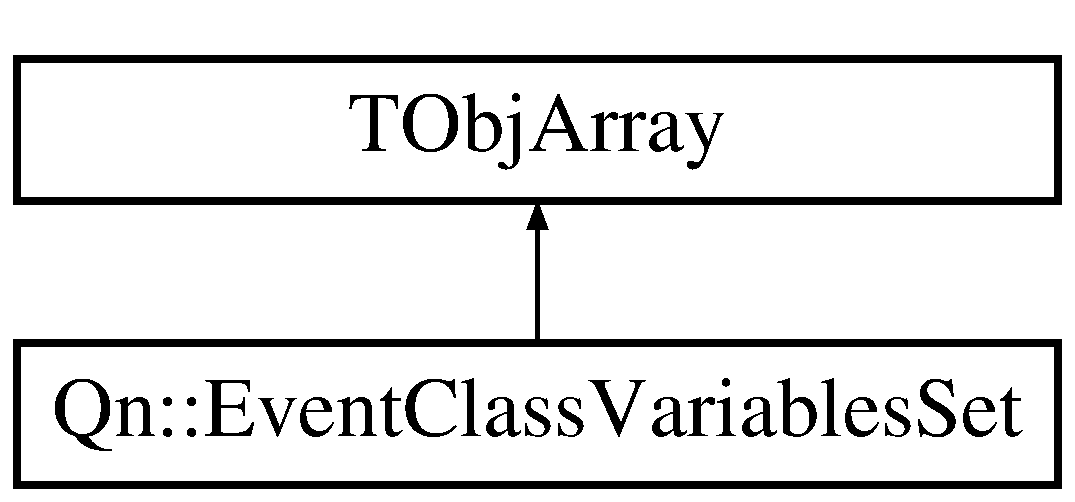
\includegraphics[height=2.000000cm]{classQn_1_1EventClassVariablesSet}
\end{center}
\end{figure}
\subsection*{Public Member Functions}
\begin{DoxyCompactItemize}
\item 
\mbox{\hyperlink{classQn_1_1EventClassVariablesSet_a8c2360e64025b5f131be1125ab36b5cb}{Event\+Class\+Variables\+Set}} (Int\+\_\+t n=T\+Collection\+::k\+Init\+Capacity)
\item 
\mbox{\hyperlink{classQn_1_1EventClassVariablesSet_a9e9e764f25f841650d6a5f053e61df77}{Event\+Class\+Variables\+Set}} (const \mbox{\hyperlink{classQn_1_1EventClassVariablesSet}{Event\+Class\+Variables\+Set}} \&cecvs)
\item 
\mbox{\Hypertarget{classQn_1_1EventClassVariablesSet_a981991d6e1983a826e8c7ac3c47fff2f}\label{classQn_1_1EventClassVariablesSet_a981991d6e1983a826e8c7ac3c47fff2f}} 
virtual \mbox{\hyperlink{classQn_1_1EventClassVariablesSet_a981991d6e1983a826e8c7ac3c47fff2f}{$\sim$\+Event\+Class\+Variables\+Set}} ()
\begin{DoxyCompactList}\small\item\em Default destructor. \end{DoxyCompactList}\item 
virtual \mbox{\hyperlink{classQn_1_1EventClassVariable}{Event\+Class\+Variable}} $\ast$ \mbox{\hyperlink{classQn_1_1EventClassVariablesSet_a774502be50fb3609d911872e0d1f3f3a}{At}} (Int\+\_\+t i) const
\item 
void \mbox{\hyperlink{classQn_1_1EventClassVariablesSet_a24d5fb123ec23c08a07268a736312593}{Get\+Multidimensional\+Configuration}} (Int\+\_\+t $\ast$nbins, Double\+\_\+t $\ast$minvals, Double\+\_\+t $\ast$maxvals)
\end{DoxyCompactItemize}


\subsection{Constructor \& Destructor Documentation}
\mbox{\Hypertarget{classQn_1_1EventClassVariablesSet_a8c2360e64025b5f131be1125ab36b5cb}\label{classQn_1_1EventClassVariablesSet_a8c2360e64025b5f131be1125ab36b5cb}} 
\index{Qn\+::\+Event\+Class\+Variables\+Set@{Qn\+::\+Event\+Class\+Variables\+Set}!Event\+Class\+Variables\+Set@{Event\+Class\+Variables\+Set}}
\index{Event\+Class\+Variables\+Set@{Event\+Class\+Variables\+Set}!Qn\+::\+Event\+Class\+Variables\+Set@{Qn\+::\+Event\+Class\+Variables\+Set}}
\subsubsection{\texorpdfstring{Event\+Class\+Variables\+Set()}{EventClassVariablesSet()}\hspace{0.1cm}{\footnotesize\ttfamily [1/2]}}
{\footnotesize\ttfamily Qn\+::\+Event\+Class\+Variables\+Set\+::\+Event\+Class\+Variables\+Set (\begin{DoxyParamCaption}\item[{Int\+\_\+t}]{n = {\ttfamily TCollection\+:\+:kInitCapacity} }\end{DoxyParamCaption})\hspace{0.3cm}{\ttfamily [inline]}}

Normal constructor 
\begin{DoxyParams}{Parameters}
{\em n} & number of variables in the set \\
\hline
\end{DoxyParams}
\mbox{\Hypertarget{classQn_1_1EventClassVariablesSet_a9e9e764f25f841650d6a5f053e61df77}\label{classQn_1_1EventClassVariablesSet_a9e9e764f25f841650d6a5f053e61df77}} 
\index{Qn\+::\+Event\+Class\+Variables\+Set@{Qn\+::\+Event\+Class\+Variables\+Set}!Event\+Class\+Variables\+Set@{Event\+Class\+Variables\+Set}}
\index{Event\+Class\+Variables\+Set@{Event\+Class\+Variables\+Set}!Qn\+::\+Event\+Class\+Variables\+Set@{Qn\+::\+Event\+Class\+Variables\+Set}}
\subsubsection{\texorpdfstring{Event\+Class\+Variables\+Set()}{EventClassVariablesSet()}\hspace{0.1cm}{\footnotesize\ttfamily [2/2]}}
{\footnotesize\ttfamily Qn\+::\+Event\+Class\+Variables\+Set\+::\+Event\+Class\+Variables\+Set (\begin{DoxyParamCaption}\item[{const \mbox{\hyperlink{classQn_1_1EventClassVariablesSet}{Event\+Class\+Variables\+Set}} \&}]{cecvs }\end{DoxyParamCaption})\hspace{0.3cm}{\ttfamily [inline]}}

Copy constructor 
\begin{DoxyParams}{Parameters}
{\em cecvs} & the object instance to be copied \\
\hline
\end{DoxyParams}


\subsection{Member Function Documentation}
\mbox{\Hypertarget{classQn_1_1EventClassVariablesSet_a774502be50fb3609d911872e0d1f3f3a}\label{classQn_1_1EventClassVariablesSet_a774502be50fb3609d911872e0d1f3f3a}} 
\index{Qn\+::\+Event\+Class\+Variables\+Set@{Qn\+::\+Event\+Class\+Variables\+Set}!At@{At}}
\index{At@{At}!Qn\+::\+Event\+Class\+Variables\+Set@{Qn\+::\+Event\+Class\+Variables\+Set}}
\subsubsection{\texorpdfstring{At()}{At()}}
{\footnotesize\ttfamily virtual \mbox{\hyperlink{classQn_1_1EventClassVariable}{Event\+Class\+Variable}}$\ast$ Qn\+::\+Event\+Class\+Variables\+Set\+::\+At (\begin{DoxyParamCaption}\item[{Int\+\_\+t}]{i }\end{DoxyParamCaption}) const\hspace{0.3cm}{\ttfamily [inline]}, {\ttfamily [virtual]}}

Access the event class variable at the passed position 
\begin{DoxyParams}{Parameters}
{\em i} & position in the array (starting at zero) \\
\hline
\end{DoxyParams}
\begin{DoxyReturn}{Returns}
the event class variable object a position i 
\end{DoxyReturn}
\mbox{\Hypertarget{classQn_1_1EventClassVariablesSet_a24d5fb123ec23c08a07268a736312593}\label{classQn_1_1EventClassVariablesSet_a24d5fb123ec23c08a07268a736312593}} 
\index{Qn\+::\+Event\+Class\+Variables\+Set@{Qn\+::\+Event\+Class\+Variables\+Set}!Get\+Multidimensional\+Configuration@{Get\+Multidimensional\+Configuration}}
\index{Get\+Multidimensional\+Configuration@{Get\+Multidimensional\+Configuration}!Qn\+::\+Event\+Class\+Variables\+Set@{Qn\+::\+Event\+Class\+Variables\+Set}}
\subsubsection{\texorpdfstring{Get\+Multidimensional\+Configuration()}{GetMultidimensionalConfiguration()}}
{\footnotesize\ttfamily void Qn\+::\+Event\+Class\+Variables\+Set\+::\+Get\+Multidimensional\+Configuration (\begin{DoxyParamCaption}\item[{Int\+\_\+t $\ast$}]{nbins,  }\item[{Double\+\_\+t $\ast$}]{minvals,  }\item[{Double\+\_\+t $\ast$}]{maxvals }\end{DoxyParamCaption})}

Gets the multidimensional configuration data

Fills the necessary information to construct a multidimensional histogram


\begin{DoxyParams}{Parameters}
{\em nbins} & storage for the number of bins of each variable \\
\hline
{\em minvals} & storage for the lower values of each variable \\
\hline
{\em maxvals} & storage for the upper values of each variable \\
\hline
\end{DoxyParams}


The documentation for this class was generated from the following files\+:\begin{DoxyCompactItemize}
\item 
D\+T\+\_\+\+Flow/\+Qn\+Corrections/include/Event\+Class\+Variables\+Set.\+h\item 
D\+T\+\_\+\+Flow/\+Qn\+Corrections/Event\+Class\+Variables\+Set.\+cpp\end{DoxyCompactItemize}

\hypertarget{classQn_1_1EventCut}{}\section{Qn\+:\+:Event\+Cut$<$ V\+AR, T $>$ Class Template Reference}
\label{classQn_1_1EventCut}\index{Qn\+::\+Event\+Cut$<$ V\+A\+R, T $>$@{Qn\+::\+Event\+Cut$<$ V\+A\+R, T $>$}}


{\ttfamily \#include $<$Event\+Cuts.\+h$>$}

Inheritance diagram for Qn\+:\+:Event\+Cut$<$ V\+AR, T $>$\+:\begin{figure}[H]
\begin{center}
\leavevmode
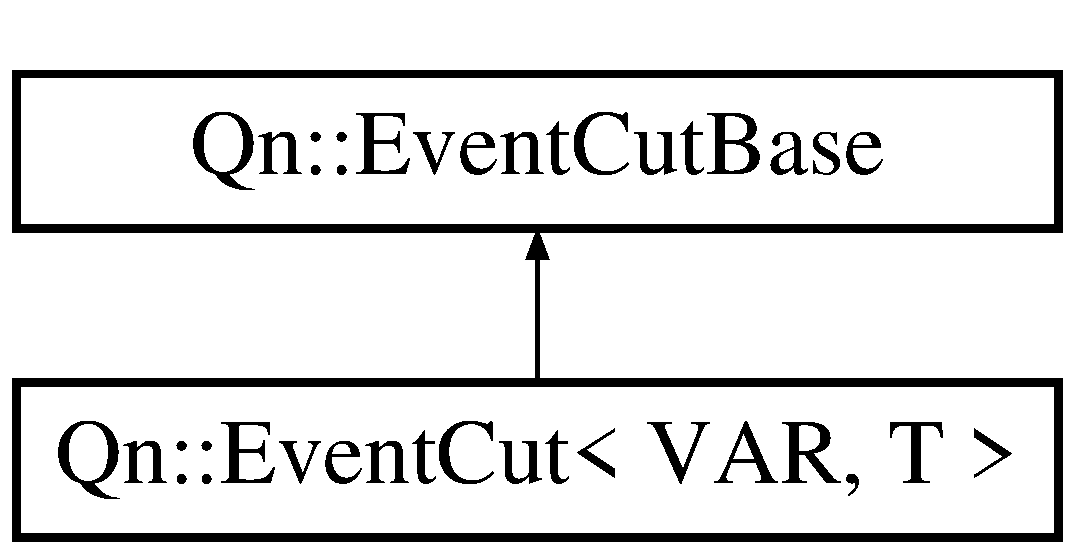
\includegraphics[height=2.000000cm]{classQn_1_1EventCut}
\end{center}
\end{figure}
\subsection*{Public Member Functions}
\begin{DoxyCompactItemize}
\item 
\mbox{\Hypertarget{classQn_1_1EventCut_a09f20d8a667327a23148d8488ea35dcd}\label{classQn_1_1EventCut_a09f20d8a667327a23148d8488ea35dcd}} 
{\bfseries Event\+Cut} (V\+AR(\&arr)\mbox{[}sizeof...(T)\mbox{]}, std\+::function$<$ bool(T...)$>$ lambda)
\item 
bool \mbox{\hyperlink{classQn_1_1EventCut_ab559f2c200401108566c1641773d778e}{Check}} () override
\item 
\mbox{\Hypertarget{classQn_1_1EventCut_a4cfeb68f1bed74e602b98df2a9ddd414}\label{classQn_1_1EventCut_a4cfeb68f1bed74e602b98df2a9ddd414}} 
std\+::string {\bfseries Name} () override
\end{DoxyCompactItemize}


\subsection{Detailed Description}
\subsubsection*{template$<$typename V\+AR, typename... T$>$\newline
class Qn\+::\+Event\+Cut$<$ V\+A\+R, T $>$}

Template class of a cut applied in the correction step. Number of dimensions is determined by the signature of the cut function and by the size of the variables array passed to the constructor. 
\begin{DoxyTemplParams}{Template Parameters}
{\em T} & Type of variable \\
\hline
\end{DoxyTemplParams}


\subsection{Member Function Documentation}
\mbox{\Hypertarget{classQn_1_1EventCut_ab559f2c200401108566c1641773d778e}\label{classQn_1_1EventCut_ab559f2c200401108566c1641773d778e}} 
\index{Qn\+::\+Event\+Cut@{Qn\+::\+Event\+Cut}!Check@{Check}}
\index{Check@{Check}!Qn\+::\+Event\+Cut@{Qn\+::\+Event\+Cut}}
\subsubsection{\texorpdfstring{Check()}{Check()}}
{\footnotesize\ttfamily template$<$typename V\+AR , typename... T$>$ \\
bool \mbox{\hyperlink{classQn_1_1EventCut}{Qn\+::\+Event\+Cut}}$<$ V\+AR, T $>$\+::Check (\begin{DoxyParamCaption}{ }\end{DoxyParamCaption})\hspace{0.3cm}{\ttfamily [inline]}, {\ttfamily [override]}, {\ttfamily [virtual]}}

Check if the cut is passed for variables at variable id + i 
\begin{DoxyParams}{Parameters}
{\em i} & offset from the variable id. \\
\hline
\end{DoxyParams}
\begin{DoxyReturn}{Returns}
true if the cut is passed. 
\end{DoxyReturn}


Implements \mbox{\hyperlink{structQn_1_1EventCutBase}{Qn\+::\+Event\+Cut\+Base}}.



The documentation for this class was generated from the following file\+:\begin{DoxyCompactItemize}
\item 
D\+T\+\_\+\+Flow/\+Correlation/include/Event\+Cuts.\+h\end{DoxyCompactItemize}

\hypertarget{structQn_1_1EventCutBase}{}\section{Qn\+:\+:Event\+Cut\+Base Struct Reference}
\label{structQn_1_1EventCutBase}\index{Qn\+::\+Event\+Cut\+Base@{Qn\+::\+Event\+Cut\+Base}}


{\ttfamily \#include $<$Event\+Cuts.\+h$>$}

Inheritance diagram for Qn\+:\+:Event\+Cut\+Base\+:\begin{figure}[H]
\begin{center}
\leavevmode
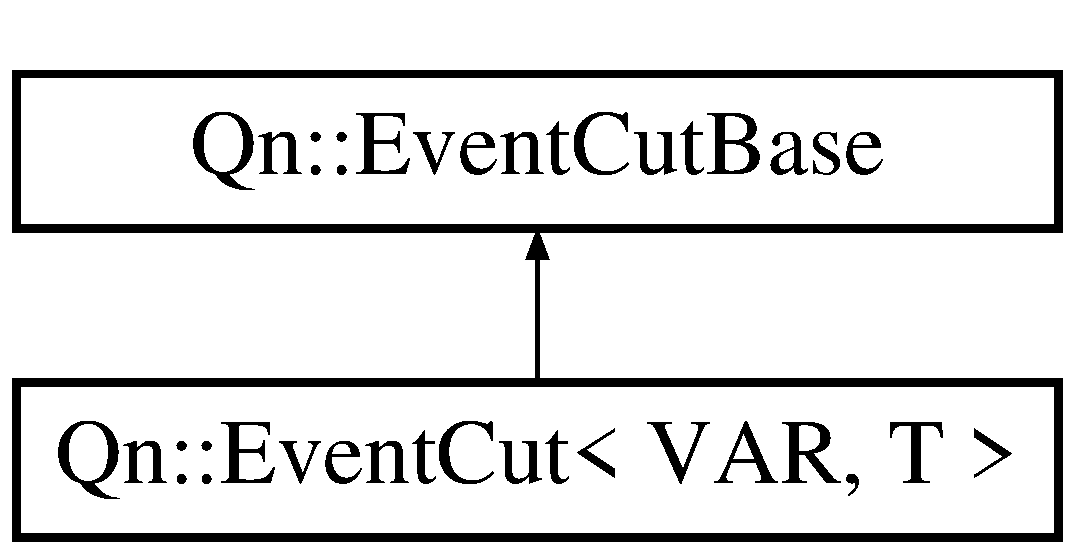
\includegraphics[height=2.000000cm]{structQn_1_1EventCutBase}
\end{center}
\end{figure}
\subsection*{Public Member Functions}
\begin{DoxyCompactItemize}
\item 
\mbox{\Hypertarget{structQn_1_1EventCutBase_a01de6b92d0ac4e6b1d9c1d4a55bf34df}\label{structQn_1_1EventCutBase_a01de6b92d0ac4e6b1d9c1d4a55bf34df}} 
virtual bool {\bfseries Check} ()=0
\item 
\mbox{\Hypertarget{structQn_1_1EventCutBase_a2c91ace130ad1d54024e1842e7ac764c}\label{structQn_1_1EventCutBase_a2c91ace130ad1d54024e1842e7ac764c}} 
virtual std\+::string {\bfseries Name} ()=0
\end{DoxyCompactItemize}


\subsection{Detailed Description}
\mbox{\hyperlink{classBase}{Base}} class of the Cut. 

The documentation for this struct was generated from the following file\+:\begin{DoxyCompactItemize}
\item 
D\+T\+\_\+\+Flow/\+Correlation/include/Event\+Cuts.\+h\end{DoxyCompactItemize}

\hypertarget{classQn_1_1EventCuts}{}\section{Qn\+:\+:Event\+Cuts Class Reference}
\label{classQn_1_1EventCuts}\index{Qn\+::\+Event\+Cuts@{Qn\+::\+Event\+Cuts}}
\subsection*{Public Member Functions}
\begin{DoxyCompactItemize}
\item 
\mbox{\Hypertarget{classQn_1_1EventCuts_affffb64a524dcb4bec6131a0230c8ef6}\label{classQn_1_1EventCuts_affffb64a524dcb4bec6131a0230c8ef6}} 
void {\bfseries Add\+Cut} (std\+::unique\+\_\+ptr$<$ \mbox{\hyperlink{structQn_1_1EventCutBase}{Event\+Cut\+Base}} $>$ cut)
\item 
\mbox{\Hypertarget{classQn_1_1EventCuts_aa3eb08d5155be6fd306e8ce24ce27e38}\label{classQn_1_1EventCuts_aa3eb08d5155be6fd306e8ce24ce27e38}} 
bool {\bfseries Check\+Cuts} ()
\item 
\mbox{\Hypertarget{classQn_1_1EventCuts_a63966f0a27f1dd066bb47f6cdafc32d5}\label{classQn_1_1EventCuts_a63966f0a27f1dd066bb47f6cdafc32d5}} 
void {\bfseries Create\+Report} ()
\item 
\mbox{\Hypertarget{classQn_1_1EventCuts_ae574bd7245c97729848a3d7ab098f281}\label{classQn_1_1EventCuts_ae574bd7245c97729848a3d7ab098f281}} 
T\+H1D $\ast$ {\bfseries Get\+Report} ()
\end{DoxyCompactItemize}


The documentation for this class was generated from the following file\+:\begin{DoxyCompactItemize}
\item 
D\+T\+\_\+\+Flow/\+Correlation/include/Event\+Cuts.\+h\end{DoxyCompactItemize}

\hypertarget{classQn_1_1EventShape}{}\section{Qn\+:\+:Event\+Shape Class Reference}
\label{classQn_1_1EventShape}\index{Qn\+::\+Event\+Shape@{Qn\+::\+Event\+Shape}}
Inheritance diagram for Qn\+:\+:Event\+Shape\+:\begin{figure}[H]
\begin{center}
\leavevmode
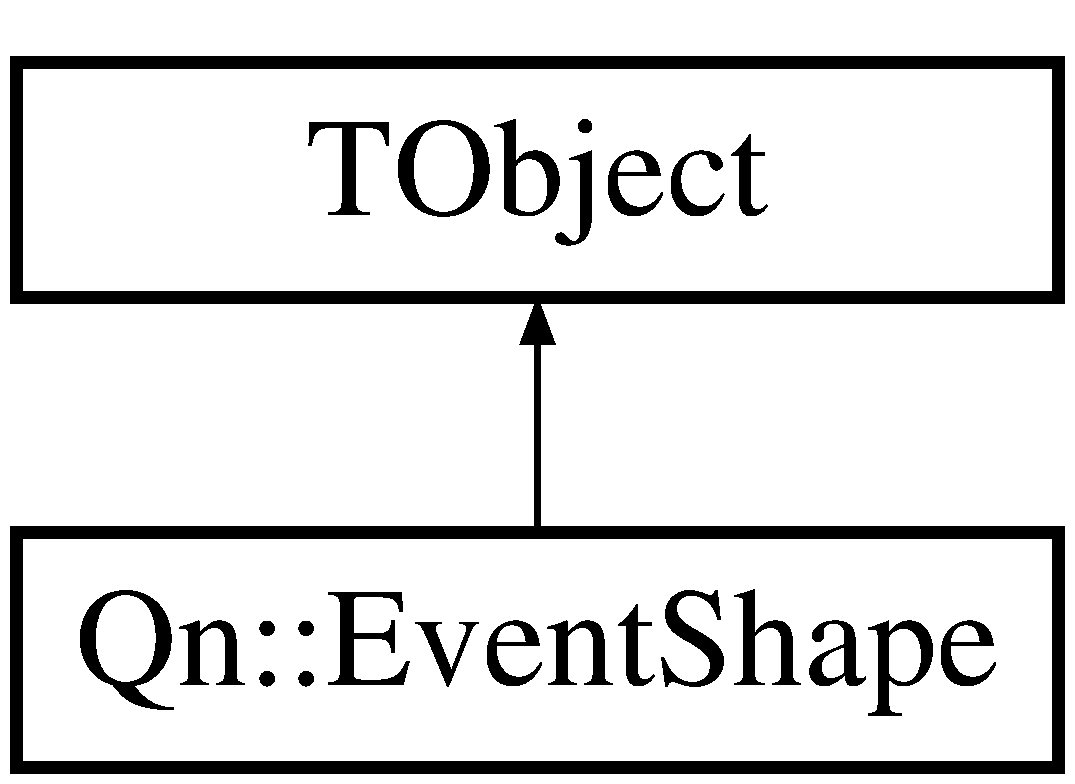
\includegraphics[height=2.000000cm]{classQn_1_1EventShape}
\end{center}
\end{figure}
\subsection*{Public Types}
\begin{DoxyCompactItemize}
\item 
enum \mbox{\hyperlink{classQn_1_1EventShape_a5dce9f7b8a7fa7a8a663634ece8b7cb6}{State}} \{ {\bfseries Uninitialized}, 
{\bfseries Ready\+For\+Collecting}, 
{\bfseries Ready\+For\+Calculation}
 \}
\end{DoxyCompactItemize}
\subsection*{Public Member Functions}
\begin{DoxyCompactItemize}
\item 
\mbox{\hyperlink{classQn_1_1EventShape_ad24dc1e3b27a1a1b476d4e46f2374f9a}{Event\+Shape}} ()=default
\item 
\mbox{\hyperlink{classQn_1_1EventShape_ac275147afb48e3eeb997626b8f7eac43}{Event\+Shape}} (std\+::string name, T\+H1F histo)
\item 
void \mbox{\hyperlink{classQn_1_1EventShape_a306f3bb8d75c6feae8b5f633a724d73e}{Set\+Histo}} (T\+H1F $\ast$histo, std\+::string name)
\item 
std\+::string \mbox{\hyperlink{classQn_1_1EventShape_abc015406701863883722b6b848fa2ac0}{Name}} () const
\item 
float \mbox{\hyperlink{classQn_1_1EventShape_a05bdd3d71c99c4a4dc192cbd861198df}{Get\+Percentile}} (float q)
\item 
void \mbox{\hyperlink{classQn_1_1EventShape_ad00484e1a53ab0e3c56eafe7f199c67b}{Integrate\+Hist}} ()
\item 
void \mbox{\hyperlink{classQn_1_1EventShape_af2c3ca720b05814421f7293fadacc312}{Fit\+With\+Spline}} ()
\item 
void \mbox{\hyperlink{classQn_1_1EventShape_a7ef94151a36c2c7ab03e5771f216a5f6}{Fill}} (const \mbox{\hyperlink{structQn_1_1Product}{Product}} \&product)
\item 
T\+H1F $\ast$ \mbox{\hyperlink{classQn_1_1EventShape_abfcccc33d6d51fdac3f72ac4039a4ad1}{Get\+Hist}} () const
\end{DoxyCompactItemize}
\subsection*{Public Attributes}
\begin{DoxyCompactItemize}
\item 
\mbox{\Hypertarget{classQn_1_1EventShape_a9391dd288a73ae2008fdf0668e8b78cb}\label{classQn_1_1EventShape_a9391dd288a73ae2008fdf0668e8b78cb}} 
std\+::string {\bfseries name\+\_\+}
\item 
\mbox{\Hypertarget{classQn_1_1EventShape_ab440a85cfe628204a36b4dd1bbcd0df3}\label{classQn_1_1EventShape_ab440a85cfe628204a36b4dd1bbcd0df3}} 
T\+Spline3 $\ast$ {\bfseries spline\+\_\+} = nullptr
\item 
\mbox{\Hypertarget{classQn_1_1EventShape_aded33163b97cd9464e4a4823bd2e0aa2}\label{classQn_1_1EventShape_aded33163b97cd9464e4a4823bd2e0aa2}} 
T\+H1F $\ast$ {\bfseries histo\+\_\+} = nullptr
\item 
\mbox{\Hypertarget{classQn_1_1EventShape_a751746c6990b00fa5dd33c63685d32f7}\label{classQn_1_1EventShape_a751746c6990b00fa5dd33c63685d32f7}} 
T\+H1F $\ast$ {\bfseries integral\+\_\+} = nullptr
\end{DoxyCompactItemize}
\subsection*{Friends}
\begin{DoxyCompactItemize}
\item 
\mbox{\Hypertarget{classQn_1_1EventShape_a3a0a26221b1b247ef5256348a0fa2ec2}\label{classQn_1_1EventShape_a3a0a26221b1b247ef5256348a0fa2ec2}} 
\mbox{\hyperlink{classQn_1_1EventShape}{Qn\+::\+Event\+Shape}} {\bfseries operator+} (const \mbox{\hyperlink{classQn_1_1EventShape}{Qn\+::\+Event\+Shape}} \&a, const \mbox{\hyperlink{classQn_1_1EventShape}{Qn\+::\+Event\+Shape}} \&b)
\item 
\mbox{\Hypertarget{classQn_1_1EventShape_a8026b1421bb3957d46d6d095a7fe3c8c}\label{classQn_1_1EventShape_a8026b1421bb3957d46d6d095a7fe3c8c}} 
\mbox{\hyperlink{classQn_1_1EventShape}{Qn\+::\+Event\+Shape}} {\bfseries Merge} (const \mbox{\hyperlink{classQn_1_1EventShape}{Qn\+::\+Event\+Shape}} \&a, const \mbox{\hyperlink{classQn_1_1EventShape}{Qn\+::\+Event\+Shape}} \&b)
\end{DoxyCompactItemize}


\subsection{Member Enumeration Documentation}
\mbox{\Hypertarget{classQn_1_1EventShape_a5dce9f7b8a7fa7a8a663634ece8b7cb6}\label{classQn_1_1EventShape_a5dce9f7b8a7fa7a8a663634ece8b7cb6}} 
\index{Qn\+::\+Event\+Shape@{Qn\+::\+Event\+Shape}!State@{State}}
\index{State@{State}!Qn\+::\+Event\+Shape@{Qn\+::\+Event\+Shape}}
\subsubsection{\texorpdfstring{State}{State}}
{\footnotesize\ttfamily enum \mbox{\hyperlink{classQn_1_1EventShape_a5dce9f7b8a7fa7a8a663634ece8b7cb6}{Qn\+::\+Event\+Shape\+::\+State}}\hspace{0.3cm}{\ttfamily [strong]}}

holds the information of the state 

\subsection{Constructor \& Destructor Documentation}
\mbox{\Hypertarget{classQn_1_1EventShape_ad24dc1e3b27a1a1b476d4e46f2374f9a}\label{classQn_1_1EventShape_ad24dc1e3b27a1a1b476d4e46f2374f9a}} 
\index{Qn\+::\+Event\+Shape@{Qn\+::\+Event\+Shape}!Event\+Shape@{Event\+Shape}}
\index{Event\+Shape@{Event\+Shape}!Qn\+::\+Event\+Shape@{Qn\+::\+Event\+Shape}}
\subsubsection{\texorpdfstring{Event\+Shape()}{EventShape()}\hspace{0.1cm}{\footnotesize\ttfamily [1/2]}}
{\footnotesize\ttfamily Qn\+::\+Event\+Shape\+::\+Event\+Shape (\begin{DoxyParamCaption}{ }\end{DoxyParamCaption})\hspace{0.3cm}{\ttfamily [default]}}

default constructor \mbox{\Hypertarget{classQn_1_1EventShape_ac275147afb48e3eeb997626b8f7eac43}\label{classQn_1_1EventShape_ac275147afb48e3eeb997626b8f7eac43}} 
\index{Qn\+::\+Event\+Shape@{Qn\+::\+Event\+Shape}!Event\+Shape@{Event\+Shape}}
\index{Event\+Shape@{Event\+Shape}!Qn\+::\+Event\+Shape@{Qn\+::\+Event\+Shape}}
\subsubsection{\texorpdfstring{Event\+Shape()}{EventShape()}\hspace{0.1cm}{\footnotesize\ttfamily [2/2]}}
{\footnotesize\ttfamily Qn\+::\+Event\+Shape\+::\+Event\+Shape (\begin{DoxyParamCaption}\item[{std\+::string}]{name,  }\item[{T\+H1F}]{histo }\end{DoxyParamCaption})\hspace{0.3cm}{\ttfamily [inline]}}

constructor 
\begin{DoxyParams}{Parameters}
{\em name} & name of the sub event \\
\hline
{\em histo} & histogram with the correct binning \\
\hline
\end{DoxyParams}


\subsection{Member Function Documentation}
\mbox{\Hypertarget{classQn_1_1EventShape_a7ef94151a36c2c7ab03e5771f216a5f6}\label{classQn_1_1EventShape_a7ef94151a36c2c7ab03e5771f216a5f6}} 
\index{Qn\+::\+Event\+Shape@{Qn\+::\+Event\+Shape}!Fill@{Fill}}
\index{Fill@{Fill}!Qn\+::\+Event\+Shape@{Qn\+::\+Event\+Shape}}
\subsubsection{\texorpdfstring{Fill()}{Fill()}}
{\footnotesize\ttfamily void Qn\+::\+Event\+Shape\+::\+Fill (\begin{DoxyParamCaption}\item[{const \mbox{\hyperlink{structQn_1_1Product}{Product}} \&}]{product }\end{DoxyParamCaption})\hspace{0.3cm}{\ttfamily [inline]}}

Fill the current subevent information to the histogram. 
\begin{DoxyParams}{Parameters}
{\em product} & \\
\hline
\end{DoxyParams}
\mbox{\Hypertarget{classQn_1_1EventShape_af2c3ca720b05814421f7293fadacc312}\label{classQn_1_1EventShape_af2c3ca720b05814421f7293fadacc312}} 
\index{Qn\+::\+Event\+Shape@{Qn\+::\+Event\+Shape}!Fit\+With\+Spline@{Fit\+With\+Spline}}
\index{Fit\+With\+Spline@{Fit\+With\+Spline}!Qn\+::\+Event\+Shape@{Qn\+::\+Event\+Shape}}
\subsubsection{\texorpdfstring{Fit\+With\+Spline()}{FitWithSpline()}}
{\footnotesize\ttfamily void Qn\+::\+Event\+Shape\+::\+Fit\+With\+Spline (\begin{DoxyParamCaption}{ }\end{DoxyParamCaption})}

Fit the histogram with a spline to calculate the percentiles. \mbox{\Hypertarget{classQn_1_1EventShape_abfcccc33d6d51fdac3f72ac4039a4ad1}\label{classQn_1_1EventShape_abfcccc33d6d51fdac3f72ac4039a4ad1}} 
\index{Qn\+::\+Event\+Shape@{Qn\+::\+Event\+Shape}!Get\+Hist@{Get\+Hist}}
\index{Get\+Hist@{Get\+Hist}!Qn\+::\+Event\+Shape@{Qn\+::\+Event\+Shape}}
\subsubsection{\texorpdfstring{Get\+Hist()}{GetHist()}}
{\footnotesize\ttfamily T\+H1F$\ast$ Qn\+::\+Event\+Shape\+::\+Get\+Hist (\begin{DoxyParamCaption}{ }\end{DoxyParamCaption}) const\hspace{0.3cm}{\ttfamily [inline]}}

Get the histogram. \begin{DoxyReturn}{Returns}
returns the distribution of all events. 
\end{DoxyReturn}
\mbox{\Hypertarget{classQn_1_1EventShape_a05bdd3d71c99c4a4dc192cbd861198df}\label{classQn_1_1EventShape_a05bdd3d71c99c4a4dc192cbd861198df}} 
\index{Qn\+::\+Event\+Shape@{Qn\+::\+Event\+Shape}!Get\+Percentile@{Get\+Percentile}}
\index{Get\+Percentile@{Get\+Percentile}!Qn\+::\+Event\+Shape@{Qn\+::\+Event\+Shape}}
\subsubsection{\texorpdfstring{Get\+Percentile()}{GetPercentile()}}
{\footnotesize\ttfamily float Qn\+::\+Event\+Shape\+::\+Get\+Percentile (\begin{DoxyParamCaption}\item[{float}]{q }\end{DoxyParamCaption})\hspace{0.3cm}{\ttfamily [inline]}}

Gets the percentile of the given q vector magnitude 
\begin{DoxyParams}{Parameters}
{\em q} & magnitude of the q vector. \\
\hline
\end{DoxyParams}
\begin{DoxyReturn}{Returns}
percentile of the current event. 
\end{DoxyReturn}
\mbox{\Hypertarget{classQn_1_1EventShape_ad00484e1a53ab0e3c56eafe7f199c67b}\label{classQn_1_1EventShape_ad00484e1a53ab0e3c56eafe7f199c67b}} 
\index{Qn\+::\+Event\+Shape@{Qn\+::\+Event\+Shape}!Integrate\+Hist@{Integrate\+Hist}}
\index{Integrate\+Hist@{Integrate\+Hist}!Qn\+::\+Event\+Shape@{Qn\+::\+Event\+Shape}}
\subsubsection{\texorpdfstring{Integrate\+Hist()}{IntegrateHist()}}
{\footnotesize\ttfamily void Qn\+::\+Event\+Shape\+::\+Integrate\+Hist (\begin{DoxyParamCaption}{ }\end{DoxyParamCaption})}

Calculate the integrated histogram of the distribution. \mbox{\Hypertarget{classQn_1_1EventShape_abc015406701863883722b6b848fa2ac0}\label{classQn_1_1EventShape_abc015406701863883722b6b848fa2ac0}} 
\index{Qn\+::\+Event\+Shape@{Qn\+::\+Event\+Shape}!Name@{Name}}
\index{Name@{Name}!Qn\+::\+Event\+Shape@{Qn\+::\+Event\+Shape}}
\subsubsection{\texorpdfstring{Name()}{Name()}}
{\footnotesize\ttfamily std\+::string Qn\+::\+Event\+Shape\+::\+Name (\begin{DoxyParamCaption}{ }\end{DoxyParamCaption}) const\hspace{0.3cm}{\ttfamily [inline]}}

Gets the name \begin{DoxyReturn}{Returns}
the name of the subevent. 
\end{DoxyReturn}
\mbox{\Hypertarget{classQn_1_1EventShape_a306f3bb8d75c6feae8b5f633a724d73e}\label{classQn_1_1EventShape_a306f3bb8d75c6feae8b5f633a724d73e}} 
\index{Qn\+::\+Event\+Shape@{Qn\+::\+Event\+Shape}!Set\+Histo@{Set\+Histo}}
\index{Set\+Histo@{Set\+Histo}!Qn\+::\+Event\+Shape@{Qn\+::\+Event\+Shape}}
\subsubsection{\texorpdfstring{Set\+Histo()}{SetHisto()}}
{\footnotesize\ttfamily void Qn\+::\+Event\+Shape\+::\+Set\+Histo (\begin{DoxyParamCaption}\item[{T\+H1F $\ast$}]{histo,  }\item[{std\+::string}]{name }\end{DoxyParamCaption})\hspace{0.3cm}{\ttfamily [inline]}}

Sets the name and binning 
\begin{DoxyParams}{Parameters}
{\em histo} & histogram with binning information \\
\hline
{\em name} & name of the subevent \\
\hline
\end{DoxyParams}


The documentation for this class was generated from the following files\+:\begin{DoxyCompactItemize}
\item 
D\+T\+\_\+\+Flow/\+Base/include/Event\+Shape.\+h\item 
D\+T\+\_\+\+Flow/\+Base/Event\+Shape.\+cpp\end{DoxyCompactItemize}

\hypertarget{classQn_1_1EventShapeResult}{}\section{Qn\+:\+:Event\+Shape\+Result Class Reference}
\label{classQn_1_1EventShapeResult}\index{Qn\+::\+Event\+Shape\+Result@{Qn\+::\+Event\+Shape\+Result}}
\subsection*{Public Types}
\begin{DoxyCompactItemize}
\item 
\mbox{\Hypertarget{classQn_1_1EventShapeResult_a21d00afbd3a0896249f23b20e6c365a0}\label{classQn_1_1EventShapeResult_a21d00afbd3a0896249f23b20e6c365a0}} 
enum {\bfseries State} \{ {\bfseries Uninitialized}, 
{\bfseries Collecting}, 
{\bfseries Calibrating}, 
{\bfseries Reading}
 \}
\end{DoxyCompactItemize}
\subsection*{Public Member Functions}
\begin{DoxyCompactItemize}
\item 
\mbox{\Hypertarget{classQn_1_1EventShapeResult_a38f78009043029a9d576ed215725c68f}\label{classQn_1_1EventShapeResult_a38f78009043029a9d576ed215725c68f}} 
{\bfseries Event\+Shape\+Result} (\mbox{\hyperlink{classQn_1_1Correlation}{Qn\+::\+Correlation}} $\ast$ptr, T\+H1F histo)
\item 
\mbox{\Hypertarget{classQn_1_1EventShapeResult_ad68afa1261a18c8c199cd18dc9c83628}\label{classQn_1_1EventShapeResult_ad68afa1261a18c8c199cd18dc9c83628}} 
{\bfseries Event\+Shape\+Result} (\mbox{\hyperlink{classQn_1_1Correlation}{Qn\+::\+Correlation}} $\ast$ptr)
\item 
\mbox{\Hypertarget{classQn_1_1EventShapeResult_a09e729415756ebf90fdecc43c8e11f6b}\label{classQn_1_1EventShapeResult_a09e729415756ebf90fdecc43c8e11f6b}} 
void {\bfseries Fit\+Splines} ()
\item 
\mbox{\Hypertarget{classQn_1_1EventShapeResult_add9cc39867a4d8bb1b18a18ab6f7ed3b}\label{classQn_1_1EventShapeResult_add9cc39867a4d8bb1b18a18ab6f7ed3b}} 
const \mbox{\hyperlink{classQn_1_1DataContainer}{Qn\+::\+Data\+Container\+Event\+Shape}} \& {\bfseries Get\+Calibration} () const
\item 
\mbox{\Hypertarget{classQn_1_1EventShapeResult_a7b74d348f97e70fd483c3cc8d9667594}\label{classQn_1_1EventShapeResult_a7b74d348f97e70fd483c3cc8d9667594}} 
void {\bfseries Configure} ()
\item 
\mbox{\Hypertarget{classQn_1_1EventShapeResult_a77f09db1049efcffa791228783bef74f}\label{classQn_1_1EventShapeResult_a77f09db1049efcffa791228783bef74f}} 
void {\bfseries Fill\+Calibration\+Histogram} ()
\item 
\mbox{\Hypertarget{classQn_1_1EventShapeResult_abdfab557a7efdad7c008f52bc440cb72}\label{classQn_1_1EventShapeResult_abdfab557a7efdad7c008f52bc440cb72}} 
double {\bfseries Get\+Percentile} (const std\+::vector$<$ unsigned long $>$ \&eventindices)
\item 
\mbox{\Hypertarget{classQn_1_1EventShapeResult_aa2ff95d57f72e0b77f2f0182cb33bad0}\label{classQn_1_1EventShapeResult_aa2ff95d57f72e0b77f2f0182cb33bad0}} 
void {\bfseries Set\+Input\+Data} (std\+::unique\+\_\+ptr$<$ \mbox{\hyperlink{classQn_1_1DataContainer}{Qn\+::\+Data\+Container\+Event\+Shape}} $>$ eventshape)
\item 
\mbox{\Hypertarget{classQn_1_1EventShapeResult_aeca1778bf874483fb3174ce4ae57f545}\label{classQn_1_1EventShapeResult_aeca1778bf874483fb3174ce4ae57f545}} 
State {\bfseries Get\+State} () const
\end{DoxyCompactItemize}


The documentation for this class was generated from the following files\+:\begin{DoxyCompactItemize}
\item 
D\+T\+\_\+\+Flow/\+Correlation/include/Event\+Shape\+Result.\+h\item 
D\+T\+\_\+\+Flow/\+Correlation/Event\+Shape\+Result.\+cpp\end{DoxyCompactItemize}

\hypertarget{classQn_1_1GainEqualization}{}\section{Qn\+:\+:Gain\+Equalization Class Reference}
\label{classQn_1_1GainEqualization}\index{Qn\+::\+Gain\+Equalization@{Qn\+::\+Gain\+Equalization}}
Inheritance diagram for Qn\+:\+:Gain\+Equalization\+:\begin{figure}[H]
\begin{center}
\leavevmode
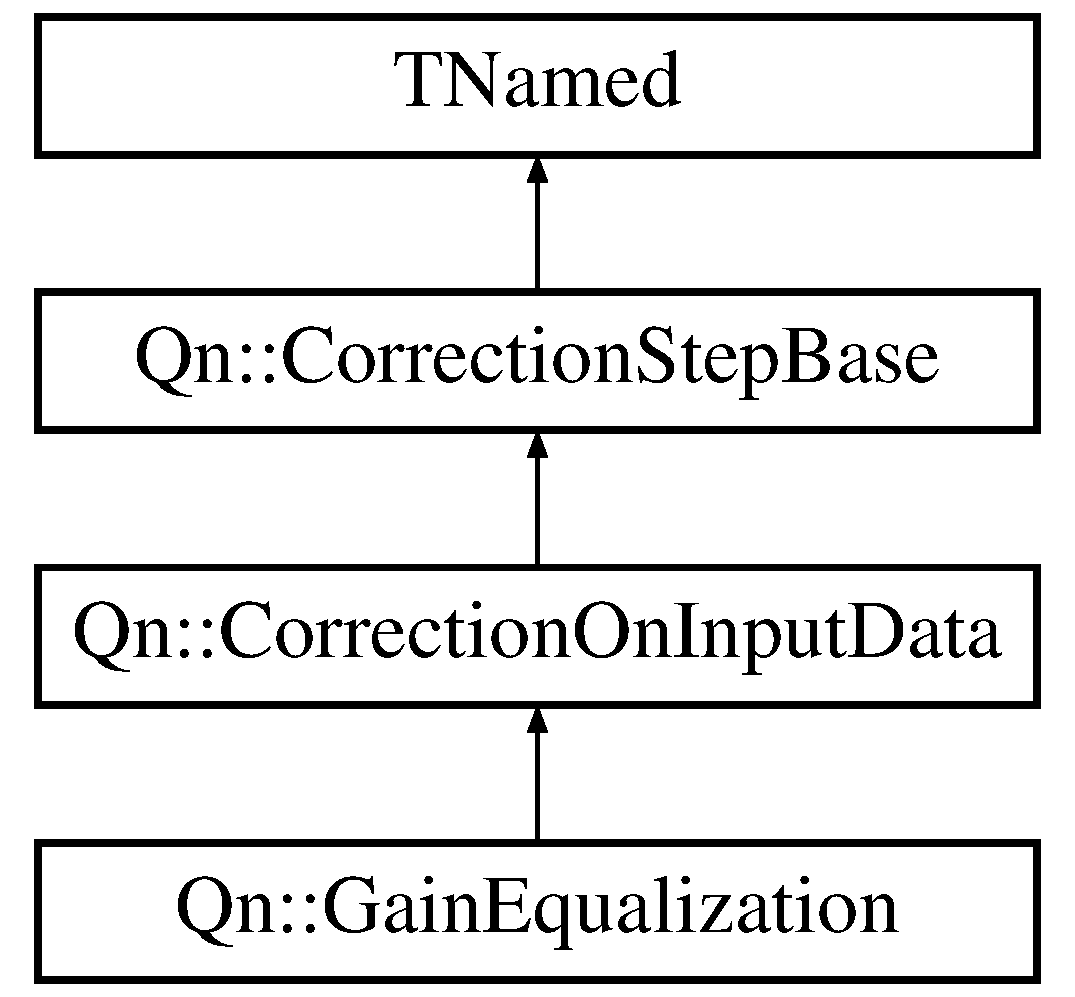
\includegraphics[height=4.000000cm]{classQn_1_1GainEqualization}
\end{center}
\end{figure}
\subsection*{Public Types}
\begin{DoxyCompactItemize}
\item 
enum \mbox{\hyperlink{classQn_1_1GainEqualization_ab49157ee7419c78638467d5a070c2c23}{Method}} \{ \mbox{\hyperlink{classQn_1_1GainEqualization_ab49157ee7419c78638467d5a070c2c23ab50339a10e1de285ac99d4c3990b8693}{Method\+::\+N\+O\+NE}}, 
\mbox{\hyperlink{classQn_1_1GainEqualization_ab49157ee7419c78638467d5a070c2c23a16de38737a9f8366e9b2042b4e9b6290}{Method\+::\+A\+V\+E\+R\+A\+GE}}, 
\mbox{\hyperlink{classQn_1_1GainEqualization_ab49157ee7419c78638467d5a070c2c23a49da85b69bc6285eeee286ca49fa7195}{Method\+::\+W\+I\+D\+TH}}
 \}
\end{DoxyCompactItemize}
\subsection*{Public Member Functions}
\begin{DoxyCompactItemize}
\item 
\mbox{\hyperlink{classQn_1_1GainEqualization_a5fc21a456890d31c36c405ed05c2e886}{Gain\+Equalization}} ()
\item 
\mbox{\hyperlink{classQn_1_1GainEqualization_a29526efb0749db5c5436edae080aea93}{$\sim$\+Gain\+Equalization}} ()
\item 
void \mbox{\hyperlink{classQn_1_1GainEqualization_a9e255e692f67af4a534017bc9d0ae630}{Set\+Equalization\+Method}} (\mbox{\hyperlink{classQn_1_1GainEqualization_ab49157ee7419c78638467d5a070c2c23}{Method}} method)
\item 
void \mbox{\hyperlink{classQn_1_1GainEqualization_acb1f9095161f3beb43d9011bc7805303}{Set\+Shift}} (Float\+\_\+t shift)
\item 
void \mbox{\hyperlink{classQn_1_1GainEqualization_a597dc9f7f5a6f7e1ec01eb907253f572}{Set\+Scale}} (Float\+\_\+t scale)
\item 
void \mbox{\hyperlink{classQn_1_1GainEqualization_af136135624a62a1372fcf31548b358d7}{Set\+Use\+Channel\+Groups\+Weights}} (Bool\+\_\+t enable)
\item 
void \mbox{\hyperlink{classQn_1_1GainEqualization_aa21fb2cf56b3fc4b7fc8d7c0c2a99da3}{Set\+No\+Of\+Entries\+Threshold}} (Int\+\_\+t n\+No\+Of\+Entries)
\item 
virtual void \mbox{\hyperlink{classQn_1_1GainEqualization_a487cc533ff299196a16d0ee4688d1039}{Attached\+To\+Framework\+Manager}} ()
\item 
virtual Bool\+\_\+t \mbox{\hyperlink{classQn_1_1GainEqualization_a167a6348fcdf8c0f48cb16a3dd9d1c29}{Attach\+Input}} (T\+List $\ast$list)
\item 
virtual void \mbox{\hyperlink{classQn_1_1GainEqualization_a3b1da6e8711ef1e7dea394d3612ee8f9}{Create\+Support\+Data\+Structures}} ()
\item 
virtual Bool\+\_\+t \mbox{\hyperlink{classQn_1_1GainEqualization_a3f34cc42fe078c556d9acf98525490ce}{Create\+Support\+Histograms}} (T\+List $\ast$list)
\item 
virtual Bool\+\_\+t \mbox{\hyperlink{classQn_1_1GainEqualization_a52c68c9bb9632a1e56341dff9e360362}{Create\+Q\+A\+Histograms}} (T\+List $\ast$list)
\item 
virtual Bool\+\_\+t \mbox{\hyperlink{classQn_1_1GainEqualization_aede344344f1f7009f10fc798cfa3241b}{Create\+Nve\+Q\+A\+Histograms}} (T\+List $\ast$list)
\item 
virtual Bool\+\_\+t \mbox{\hyperlink{classQn_1_1GainEqualization_ade22bc9b3aee596b6594d8a8d6fdc1f1}{Process\+Corrections}} (const double $\ast$variable\+Container)
\item 
virtual Bool\+\_\+t \mbox{\hyperlink{classQn_1_1GainEqualization_a9984ec9a1056bc3e336ff9ac50888641}{Process\+Data\+Collection}} (const double $\ast$variable\+Container)
\item 
virtual void \mbox{\hyperlink{classQn_1_1GainEqualization_a8ee1f2ecf6929de35d455515a067ac9c}{Clear\+Correction\+Step}} ()
\item 
virtual Bool\+\_\+t \mbox{\hyperlink{classQn_1_1GainEqualization_af444038af10eb53d8bd6c8703d4e5629}{Report\+Usage}} (T\+List $\ast$calibration\+List, T\+List $\ast$apply\+List)
\end{DoxyCompactItemize}
\subsection*{Additional Inherited Members}


\subsection{Member Enumeration Documentation}
\mbox{\Hypertarget{classQn_1_1GainEqualization_ab49157ee7419c78638467d5a070c2c23}\label{classQn_1_1GainEqualization_ab49157ee7419c78638467d5a070c2c23}} 
\index{Qn\+::\+Gain\+Equalization@{Qn\+::\+Gain\+Equalization}!Method@{Method}}
\index{Method@{Method}!Qn\+::\+Gain\+Equalization@{Qn\+::\+Gain\+Equalization}}
\subsubsection{\texorpdfstring{Method}{Method}}
{\footnotesize\ttfamily enum \mbox{\hyperlink{classQn_1_1GainEqualization_ab49157ee7419c78638467d5a070c2c23}{Qn\+::\+Gain\+Equalization\+::\+Method}}\hspace{0.3cm}{\ttfamily [strong]}}

\begin{DoxyEnumFields}{Enumerator}
\raisebox{\heightof{T}}[0pt][0pt]{\index{N\+O\+NE@{N\+O\+NE}!Qn\+::\+Gain\+Equalization@{Qn\+::\+Gain\+Equalization}}\index{Qn\+::\+Gain\+Equalization@{Qn\+::\+Gain\+Equalization}!N\+O\+NE@{N\+O\+NE}}}\mbox{\Hypertarget{classQn_1_1GainEqualization_ab49157ee7419c78638467d5a070c2c23ab50339a10e1de285ac99d4c3990b8693}\label{classQn_1_1GainEqualization_ab49157ee7419c78638467d5a070c2c23ab50339a10e1de285ac99d4c3990b8693}} 
N\+O\+NE&$ \mbox{M'} = \mbox{M}$ \\
\hline

\raisebox{\heightof{T}}[0pt][0pt]{\index{A\+V\+E\+R\+A\+GE@{A\+V\+E\+R\+A\+GE}!Qn\+::\+Gain\+Equalization@{Qn\+::\+Gain\+Equalization}}\index{Qn\+::\+Gain\+Equalization@{Qn\+::\+Gain\+Equalization}!A\+V\+E\+R\+A\+GE@{A\+V\+E\+R\+A\+GE}}}\mbox{\Hypertarget{classQn_1_1GainEqualization_ab49157ee7419c78638467d5a070c2c23a16de38737a9f8366e9b2042b4e9b6290}\label{classQn_1_1GainEqualization_ab49157ee7419c78638467d5a070c2c23a16de38737a9f8366e9b2042b4e9b6290}} 
A\+V\+E\+R\+A\+GE&$ \mbox{M}' = \frac{\mbox{M}}{\langle\mbox{M}\rangle} $ \\
\hline

\raisebox{\heightof{T}}[0pt][0pt]{\index{W\+I\+D\+TH@{W\+I\+D\+TH}!Qn\+::\+Gain\+Equalization@{Qn\+::\+Gain\+Equalization}}\index{Qn\+::\+Gain\+Equalization@{Qn\+::\+Gain\+Equalization}!W\+I\+D\+TH@{W\+I\+D\+TH}}}\mbox{\Hypertarget{classQn_1_1GainEqualization_ab49157ee7419c78638467d5a070c2c23a49da85b69bc6285eeee286ca49fa7195}\label{classQn_1_1GainEqualization_ab49157ee7419c78638467d5a070c2c23a49da85b69bc6285eeee286ca49fa7195}} 
W\+I\+D\+TH&$ \mbox{M}' = \mbox{A} + \mbox{B} \frac{\mbox{M} - \langle\mbox{M} \rangle}{\sigma_{{M}}} $ \\
\hline

\end{DoxyEnumFields}


\subsection{Constructor \& Destructor Documentation}
\mbox{\Hypertarget{classQn_1_1GainEqualization_a5fc21a456890d31c36c405ed05c2e886}\label{classQn_1_1GainEqualization_a5fc21a456890d31c36c405ed05c2e886}} 
\index{Qn\+::\+Gain\+Equalization@{Qn\+::\+Gain\+Equalization}!Gain\+Equalization@{Gain\+Equalization}}
\index{Gain\+Equalization@{Gain\+Equalization}!Qn\+::\+Gain\+Equalization@{Qn\+::\+Gain\+Equalization}}
\subsubsection{\texorpdfstring{Gain\+Equalization()}{GainEqualization()}}
{\footnotesize\ttfamily Qn\+::\+Gain\+Equalization\+::\+Gain\+Equalization (\begin{DoxyParamCaption}{ }\end{DoxyParamCaption})}

Default constructor Passes to the base class the identity data for the Gain equalization correction step \mbox{\Hypertarget{classQn_1_1GainEqualization_a29526efb0749db5c5436edae080aea93}\label{classQn_1_1GainEqualization_a29526efb0749db5c5436edae080aea93}} 
\index{Qn\+::\+Gain\+Equalization@{Qn\+::\+Gain\+Equalization}!````~Gain\+Equalization@{$\sim$\+Gain\+Equalization}}
\index{````~Gain\+Equalization@{$\sim$\+Gain\+Equalization}!Qn\+::\+Gain\+Equalization@{Qn\+::\+Gain\+Equalization}}
\subsubsection{\texorpdfstring{$\sim$\+Gain\+Equalization()}{~GainEqualization()}}
{\footnotesize\ttfamily Qn\+::\+Gain\+Equalization\+::$\sim$\+Gain\+Equalization (\begin{DoxyParamCaption}{ }\end{DoxyParamCaption})}

Default destructor Releases the memory taken 

\subsection{Member Function Documentation}
\mbox{\Hypertarget{classQn_1_1GainEqualization_a487cc533ff299196a16d0ee4688d1039}\label{classQn_1_1GainEqualization_a487cc533ff299196a16d0ee4688d1039}} 
\index{Qn\+::\+Gain\+Equalization@{Qn\+::\+Gain\+Equalization}!Attached\+To\+Framework\+Manager@{Attached\+To\+Framework\+Manager}}
\index{Attached\+To\+Framework\+Manager@{Attached\+To\+Framework\+Manager}!Qn\+::\+Gain\+Equalization@{Qn\+::\+Gain\+Equalization}}
\subsubsection{\texorpdfstring{Attached\+To\+Framework\+Manager()}{AttachedToFrameworkManager()}}
{\footnotesize\ttfamily virtual void Qn\+::\+Gain\+Equalization\+::\+Attached\+To\+Framework\+Manager (\begin{DoxyParamCaption}{ }\end{DoxyParamCaption})\hspace{0.3cm}{\ttfamily [inline]}, {\ttfamily [virtual]}}

Informs when the detector configuration has been attached to the framework manager Basically this allows interaction between the different framework sections at configuration time No action for input gain equalization 

Implements \mbox{\hyperlink{classQn_1_1CorrectionOnInputData_adab1d79e0c216c6c981cd8d7ed271490}{Qn\+::\+Correction\+On\+Input\+Data}}.

\mbox{\Hypertarget{classQn_1_1GainEqualization_a167a6348fcdf8c0f48cb16a3dd9d1c29}\label{classQn_1_1GainEqualization_a167a6348fcdf8c0f48cb16a3dd9d1c29}} 
\index{Qn\+::\+Gain\+Equalization@{Qn\+::\+Gain\+Equalization}!Attach\+Input@{Attach\+Input}}
\index{Attach\+Input@{Attach\+Input}!Qn\+::\+Gain\+Equalization@{Qn\+::\+Gain\+Equalization}}
\subsubsection{\texorpdfstring{Attach\+Input()}{AttachInput()}}
{\footnotesize\ttfamily Bool\+\_\+t Qn\+::\+Gain\+Equalization\+::\+Attach\+Input (\begin{DoxyParamCaption}\item[{T\+List $\ast$}]{list }\end{DoxyParamCaption})\hspace{0.3cm}{\ttfamily [virtual]}}

Attaches the needed input information to the correction step

If the attachment succeeded asks for hard coded group weights to the detector configuration 
\begin{DoxyParams}{Parameters}
{\em list} & list where the inputs should be found \\
\hline
\end{DoxyParams}
\begin{DoxyReturn}{Returns}
k\+T\+R\+UE if everything went OK 
\end{DoxyReturn}


Implements \mbox{\hyperlink{classQn_1_1CorrectionOnInputData_a37c53966c0121ed0f7d764a9769690be}{Qn\+::\+Correction\+On\+Input\+Data}}.

\mbox{\Hypertarget{classQn_1_1GainEqualization_a8ee1f2ecf6929de35d455515a067ac9c}\label{classQn_1_1GainEqualization_a8ee1f2ecf6929de35d455515a067ac9c}} 
\index{Qn\+::\+Gain\+Equalization@{Qn\+::\+Gain\+Equalization}!Clear\+Correction\+Step@{Clear\+Correction\+Step}}
\index{Clear\+Correction\+Step@{Clear\+Correction\+Step}!Qn\+::\+Gain\+Equalization@{Qn\+::\+Gain\+Equalization}}
\subsubsection{\texorpdfstring{Clear\+Correction\+Step()}{ClearCorrectionStep()}}
{\footnotesize\ttfamily virtual void Qn\+::\+Gain\+Equalization\+::\+Clear\+Correction\+Step (\begin{DoxyParamCaption}{ }\end{DoxyParamCaption})\hspace{0.3cm}{\ttfamily [inline]}, {\ttfamily [virtual]}}

Clean the correction to accept a new event Does nothing for the time being 

Implements \mbox{\hyperlink{classQn_1_1CorrectionOnInputData_a8da92a3389c8654961199f123d5e6a6d}{Qn\+::\+Correction\+On\+Input\+Data}}.

\mbox{\Hypertarget{classQn_1_1GainEqualization_aede344344f1f7009f10fc798cfa3241b}\label{classQn_1_1GainEqualization_aede344344f1f7009f10fc798cfa3241b}} 
\index{Qn\+::\+Gain\+Equalization@{Qn\+::\+Gain\+Equalization}!Create\+Nve\+Q\+A\+Histograms@{Create\+Nve\+Q\+A\+Histograms}}
\index{Create\+Nve\+Q\+A\+Histograms@{Create\+Nve\+Q\+A\+Histograms}!Qn\+::\+Gain\+Equalization@{Qn\+::\+Gain\+Equalization}}
\subsubsection{\texorpdfstring{Create\+Nve\+Q\+A\+Histograms()}{CreateNveQAHistograms()}}
{\footnotesize\ttfamily Bool\+\_\+t Qn\+::\+Gain\+Equalization\+::\+Create\+Nve\+Q\+A\+Histograms (\begin{DoxyParamCaption}\item[{T\+List $\ast$}]{list }\end{DoxyParamCaption})\hspace{0.3cm}{\ttfamily [virtual]}}

Asks for non validated entries QA histograms creation

Allocates the histogram objects and creates the non validated entries QA histograms. 
\begin{DoxyParams}{Parameters}
{\em list} & list where the histograms should be incorporated for its persistence \\
\hline
\end{DoxyParams}
\begin{DoxyReturn}{Returns}
k\+T\+R\+UE if everything went OK 
\end{DoxyReturn}


Implements \mbox{\hyperlink{classQn_1_1CorrectionStepBase_acb488e715005f027e39c21ae5f4684da}{Qn\+::\+Correction\+Step\+Base}}.

\mbox{\Hypertarget{classQn_1_1GainEqualization_a52c68c9bb9632a1e56341dff9e360362}\label{classQn_1_1GainEqualization_a52c68c9bb9632a1e56341dff9e360362}} 
\index{Qn\+::\+Gain\+Equalization@{Qn\+::\+Gain\+Equalization}!Create\+Q\+A\+Histograms@{Create\+Q\+A\+Histograms}}
\index{Create\+Q\+A\+Histograms@{Create\+Q\+A\+Histograms}!Qn\+::\+Gain\+Equalization@{Qn\+::\+Gain\+Equalization}}
\subsubsection{\texorpdfstring{Create\+Q\+A\+Histograms()}{CreateQAHistograms()}}
{\footnotesize\ttfamily Bool\+\_\+t Qn\+::\+Gain\+Equalization\+::\+Create\+Q\+A\+Histograms (\begin{DoxyParamCaption}\item[{T\+List $\ast$}]{list }\end{DoxyParamCaption})\hspace{0.3cm}{\ttfamily [virtual]}}

Asks for QA histograms creation

Allocates the histogram objects and creates the QA histograms. 
\begin{DoxyParams}{Parameters}
{\em list} & list where the histograms should be incorporated for its persistence \\
\hline
\end{DoxyParams}
\begin{DoxyReturn}{Returns}
k\+T\+R\+UE if everything went OK 
\end{DoxyReturn}


Implements \mbox{\hyperlink{classQn_1_1CorrectionStepBase_a21f58f5d91209c1c74d0928cf0b3e26d}{Qn\+::\+Correction\+Step\+Base}}.

\mbox{\Hypertarget{classQn_1_1GainEqualization_a3b1da6e8711ef1e7dea394d3612ee8f9}\label{classQn_1_1GainEqualization_a3b1da6e8711ef1e7dea394d3612ee8f9}} 
\index{Qn\+::\+Gain\+Equalization@{Qn\+::\+Gain\+Equalization}!Create\+Support\+Data\+Structures@{Create\+Support\+Data\+Structures}}
\index{Create\+Support\+Data\+Structures@{Create\+Support\+Data\+Structures}!Qn\+::\+Gain\+Equalization@{Qn\+::\+Gain\+Equalization}}
\subsubsection{\texorpdfstring{Create\+Support\+Data\+Structures()}{CreateSupportDataStructures()}}
{\footnotesize\ttfamily void Qn\+::\+Gain\+Equalization\+::\+Create\+Support\+Data\+Structures (\begin{DoxyParamCaption}{ }\end{DoxyParamCaption})\hspace{0.3cm}{\ttfamily [virtual]}}

Asks for support data structures creation

Does nothing for the time being 

Implements \mbox{\hyperlink{classQn_1_1CorrectionOnInputData_a7da5cb5e6c82e28e2dd63d82ac82bc8a}{Qn\+::\+Correction\+On\+Input\+Data}}.

\mbox{\Hypertarget{classQn_1_1GainEqualization_a3f34cc42fe078c556d9acf98525490ce}\label{classQn_1_1GainEqualization_a3f34cc42fe078c556d9acf98525490ce}} 
\index{Qn\+::\+Gain\+Equalization@{Qn\+::\+Gain\+Equalization}!Create\+Support\+Histograms@{Create\+Support\+Histograms}}
\index{Create\+Support\+Histograms@{Create\+Support\+Histograms}!Qn\+::\+Gain\+Equalization@{Qn\+::\+Gain\+Equalization}}
\subsubsection{\texorpdfstring{Create\+Support\+Histograms()}{CreateSupportHistograms()}}
{\footnotesize\ttfamily Bool\+\_\+t Qn\+::\+Gain\+Equalization\+::\+Create\+Support\+Histograms (\begin{DoxyParamCaption}\item[{T\+List $\ast$}]{list }\end{DoxyParamCaption})\hspace{0.3cm}{\ttfamily [virtual]}}

Asks for support histograms creation

Allocates the histogram objects and creates the calibration histograms. The histograms are constructed with standard deviation error calculation for the proper behavior of the gain equalization.

Process concurrency requires Calibration Histograms creation for all c concurrent processes but not for Input Histograms so, we delete previously allocated ones. 
\begin{DoxyParams}{Parameters}
{\em list} & list where the histograms should be incorporated for its persistence \\
\hline
\end{DoxyParams}
\begin{DoxyReturn}{Returns}
k\+T\+R\+UE if everything went OK 
\end{DoxyReturn}


Implements \mbox{\hyperlink{classQn_1_1CorrectionOnInputData_a1556dd574545ef77d6b462020101bf39}{Qn\+::\+Correction\+On\+Input\+Data}}.

\mbox{\Hypertarget{classQn_1_1GainEqualization_ade22bc9b3aee596b6594d8a8d6fdc1f1}\label{classQn_1_1GainEqualization_ade22bc9b3aee596b6594d8a8d6fdc1f1}} 
\index{Qn\+::\+Gain\+Equalization@{Qn\+::\+Gain\+Equalization}!Process\+Corrections@{Process\+Corrections}}
\index{Process\+Corrections@{Process\+Corrections}!Qn\+::\+Gain\+Equalization@{Qn\+::\+Gain\+Equalization}}
\subsubsection{\texorpdfstring{Process\+Corrections()}{ProcessCorrections()}}
{\footnotesize\ttfamily Bool\+\_\+t Qn\+::\+Gain\+Equalization\+::\+Process\+Corrections (\begin{DoxyParamCaption}\item[{const double $\ast$}]{variable\+Container }\end{DoxyParamCaption})\hspace{0.3cm}{\ttfamily [virtual]}}

Processes the correction step

Data are always taken from the data bank from the equalized weights allowing chaining of input data corrections so, caution must be taken to be sure that, on initialising, weight and equalized weight match Due to this structure as today it is not possible to split data collection from correction processing. If so is required probably multiple equalization structures should be included. \begin{DoxyReturn}{Returns}
k\+T\+R\+UE if the correction step was applied 
\end{DoxyReturn}


Implements \mbox{\hyperlink{classQn_1_1CorrectionOnInputData_a42390a6c47f558faeb1e14d245dcbc4a}{Qn\+::\+Correction\+On\+Input\+Data}}.

\mbox{\Hypertarget{classQn_1_1GainEqualization_a9984ec9a1056bc3e336ff9ac50888641}\label{classQn_1_1GainEqualization_a9984ec9a1056bc3e336ff9ac50888641}} 
\index{Qn\+::\+Gain\+Equalization@{Qn\+::\+Gain\+Equalization}!Process\+Data\+Collection@{Process\+Data\+Collection}}
\index{Process\+Data\+Collection@{Process\+Data\+Collection}!Qn\+::\+Gain\+Equalization@{Qn\+::\+Gain\+Equalization}}
\subsubsection{\texorpdfstring{Process\+Data\+Collection()}{ProcessDataCollection()}}
{\footnotesize\ttfamily Bool\+\_\+t Qn\+::\+Gain\+Equalization\+::\+Process\+Data\+Collection (\begin{DoxyParamCaption}\item[{const double $\ast$}]{variable\+Container }\end{DoxyParamCaption})\hspace{0.3cm}{\ttfamily [virtual]}}

Processes the correction data collection step

Data are always taken from the data bank from the equalized weights allowing chaining of input data corrections so, caution must be taken to be sure that, on initialising, weight and equalized weight match Due to this structure as today it is not possible to split data collection from correction processing. If so is required probably multiple equalization structures should be included. So this function only retures the proper value according to the status. \begin{DoxyReturn}{Returns}
k\+T\+R\+UE if the correction step was applied 
\end{DoxyReturn}


Implements \mbox{\hyperlink{classQn_1_1CorrectionOnInputData_aff000eb0dbd571ac42eb0c4d3771ba69}{Qn\+::\+Correction\+On\+Input\+Data}}.

\mbox{\Hypertarget{classQn_1_1GainEqualization_af444038af10eb53d8bd6c8703d4e5629}\label{classQn_1_1GainEqualization_af444038af10eb53d8bd6c8703d4e5629}} 
\index{Qn\+::\+Gain\+Equalization@{Qn\+::\+Gain\+Equalization}!Report\+Usage@{Report\+Usage}}
\index{Report\+Usage@{Report\+Usage}!Qn\+::\+Gain\+Equalization@{Qn\+::\+Gain\+Equalization}}
\subsubsection{\texorpdfstring{Report\+Usage()}{ReportUsage()}}
{\footnotesize\ttfamily Bool\+\_\+t Qn\+::\+Gain\+Equalization\+::\+Report\+Usage (\begin{DoxyParamCaption}\item[{T\+List $\ast$}]{calibration\+List,  }\item[{T\+List $\ast$}]{apply\+List }\end{DoxyParamCaption})\hspace{0.3cm}{\ttfamily [virtual]}}

Report on correction usage Correction step should incorporate its name in calibration list if it is producing information calibration in the ongoing step and in the apply list if it is applying correction in the ongoing step. 
\begin{DoxyParams}{Parameters}
{\em calibration\+List} & list containing the correction steps producing calibration information \\
\hline
{\em apply\+List} & list containing the correction steps applying corrections \\
\hline
\end{DoxyParams}
\begin{DoxyReturn}{Returns}
k\+T\+R\+UE if the correction step is being applied 
\end{DoxyReturn}


Implements \mbox{\hyperlink{classQn_1_1CorrectionOnInputData_a40b05b6db47e8dd52e1f6a616b9b9d3a}{Qn\+::\+Correction\+On\+Input\+Data}}.

\mbox{\Hypertarget{classQn_1_1GainEqualization_a9e255e692f67af4a534017bc9d0ae630}\label{classQn_1_1GainEqualization_a9e255e692f67af4a534017bc9d0ae630}} 
\index{Qn\+::\+Gain\+Equalization@{Qn\+::\+Gain\+Equalization}!Set\+Equalization\+Method@{Set\+Equalization\+Method}}
\index{Set\+Equalization\+Method@{Set\+Equalization\+Method}!Qn\+::\+Gain\+Equalization@{Qn\+::\+Gain\+Equalization}}
\subsubsection{\texorpdfstring{Set\+Equalization\+Method()}{SetEqualizationMethod()}}
{\footnotesize\ttfamily void Qn\+::\+Gain\+Equalization\+::\+Set\+Equalization\+Method (\begin{DoxyParamCaption}\item[{\mbox{\hyperlink{classQn_1_1GainEqualization_ab49157ee7419c78638467d5a070c2c23}{Method}}}]{method }\end{DoxyParamCaption})\hspace{0.3cm}{\ttfamily [inline]}}

Stores the passed equalization method 
\begin{DoxyParams}{Parameters}
{\em method} & the desired equalization method \\
\hline
\end{DoxyParams}
\mbox{\Hypertarget{classQn_1_1GainEqualization_aa21fb2cf56b3fc4b7fc8d7c0c2a99da3}\label{classQn_1_1GainEqualization_aa21fb2cf56b3fc4b7fc8d7c0c2a99da3}} 
\index{Qn\+::\+Gain\+Equalization@{Qn\+::\+Gain\+Equalization}!Set\+No\+Of\+Entries\+Threshold@{Set\+No\+Of\+Entries\+Threshold}}
\index{Set\+No\+Of\+Entries\+Threshold@{Set\+No\+Of\+Entries\+Threshold}!Qn\+::\+Gain\+Equalization@{Qn\+::\+Gain\+Equalization}}
\subsubsection{\texorpdfstring{Set\+No\+Of\+Entries\+Threshold()}{SetNoOfEntriesThreshold()}}
{\footnotesize\ttfamily void Qn\+::\+Gain\+Equalization\+::\+Set\+No\+Of\+Entries\+Threshold (\begin{DoxyParamCaption}\item[{Int\+\_\+t}]{n\+No\+Of\+Entries }\end{DoxyParamCaption})\hspace{0.3cm}{\ttfamily [inline]}}

Set the minimum number of entries for calibration histogram bin content validation 
\begin{DoxyParams}{Parameters}
{\em n\+No\+Of\+Entries} & the number of entries threshold \\
\hline
\end{DoxyParams}
\mbox{\Hypertarget{classQn_1_1GainEqualization_a597dc9f7f5a6f7e1ec01eb907253f572}\label{classQn_1_1GainEqualization_a597dc9f7f5a6f7e1ec01eb907253f572}} 
\index{Qn\+::\+Gain\+Equalization@{Qn\+::\+Gain\+Equalization}!Set\+Scale@{Set\+Scale}}
\index{Set\+Scale@{Set\+Scale}!Qn\+::\+Gain\+Equalization@{Qn\+::\+Gain\+Equalization}}
\subsubsection{\texorpdfstring{Set\+Scale()}{SetScale()}}
{\footnotesize\ttfamily void Qn\+::\+Gain\+Equalization\+::\+Set\+Scale (\begin{DoxyParamCaption}\item[{Float\+\_\+t}]{scale }\end{DoxyParamCaption})\hspace{0.3cm}{\ttfamily [inline]}}

Set the scale (B) equalization parameter 
\begin{DoxyParams}{Parameters}
{\em scale} & the scale parameter value \\
\hline
\end{DoxyParams}
\mbox{\Hypertarget{classQn_1_1GainEqualization_acb1f9095161f3beb43d9011bc7805303}\label{classQn_1_1GainEqualization_acb1f9095161f3beb43d9011bc7805303}} 
\index{Qn\+::\+Gain\+Equalization@{Qn\+::\+Gain\+Equalization}!Set\+Shift@{Set\+Shift}}
\index{Set\+Shift@{Set\+Shift}!Qn\+::\+Gain\+Equalization@{Qn\+::\+Gain\+Equalization}}
\subsubsection{\texorpdfstring{Set\+Shift()}{SetShift()}}
{\footnotesize\ttfamily void Qn\+::\+Gain\+Equalization\+::\+Set\+Shift (\begin{DoxyParamCaption}\item[{Float\+\_\+t}]{shift }\end{DoxyParamCaption})\hspace{0.3cm}{\ttfamily [inline]}}

Set the shift (A) width equalization parameter 
\begin{DoxyParams}{Parameters}
{\em shift} & the shift parameter value \\
\hline
\end{DoxyParams}
\mbox{\Hypertarget{classQn_1_1GainEqualization_af136135624a62a1372fcf31548b358d7}\label{classQn_1_1GainEqualization_af136135624a62a1372fcf31548b358d7}} 
\index{Qn\+::\+Gain\+Equalization@{Qn\+::\+Gain\+Equalization}!Set\+Use\+Channel\+Groups\+Weights@{Set\+Use\+Channel\+Groups\+Weights}}
\index{Set\+Use\+Channel\+Groups\+Weights@{Set\+Use\+Channel\+Groups\+Weights}!Qn\+::\+Gain\+Equalization@{Qn\+::\+Gain\+Equalization}}
\subsubsection{\texorpdfstring{Set\+Use\+Channel\+Groups\+Weights()}{SetUseChannelGroupsWeights()}}
{\footnotesize\ttfamily void Qn\+::\+Gain\+Equalization\+::\+Set\+Use\+Channel\+Groups\+Weights (\begin{DoxyParamCaption}\item[{Bool\+\_\+t}]{enable }\end{DoxyParamCaption})\hspace{0.3cm}{\ttfamily [inline]}}

Enable or disable the group weights extracted from channel multiplicity 
\begin{DoxyParams}{Parameters}
{\em enable} & k\+T\+R\+UE / k\+F\+A\+L\+SE for enable / disable it \\
\hline
\end{DoxyParams}


The documentation for this class was generated from the following files\+:\begin{DoxyCompactItemize}
\item 
D\+T\+\_\+\+Flow/\+Qn\+Corrections/include/Gain\+Equalization.\+h\item 
D\+T\+\_\+\+Flow/\+Qn\+Corrections/Gain\+Equalization.\+cpp\end{DoxyCompactItemize}

\hypertarget{classHolds}{}\section{Holds Class Reference}
\label{classHolds}\index{Holds@{Holds}}


\subsection{Detailed Description}
information. Can be saved to a file. 

The documentation for this class was generated from the following file\+:\begin{DoxyCompactItemize}
\item 
D\+T\+\_\+\+Flow/\+Base/include/Event\+Shape.\+h\end{DoxyCompactItemize}

\hypertarget{structstd_1_1less_3_01Qn_1_1Variable_01_4}{}\section{std\+:\+:less$<$ Qn\+:\+:Variable $>$ Struct Template Reference}
\label{structstd_1_1less_3_01Qn_1_1Variable_01_4}\index{std\+::less$<$ Qn\+::\+Variable $>$@{std\+::less$<$ Qn\+::\+Variable $>$}}


{\ttfamily \#include $<$Variable\+Manager.\+h$>$}

\subsection*{Public Member Functions}
\begin{DoxyCompactItemize}
\item 
\mbox{\Hypertarget{structstd_1_1less_3_01Qn_1_1Variable_01_4_ad63cb583e698381109e45a5dfdf12d3b}\label{structstd_1_1less_3_01Qn_1_1Variable_01_4_ad63cb583e698381109e45a5dfdf12d3b}} 
bool {\bfseries operator()} (const \mbox{\hyperlink{classQn_1_1Variable}{Qn\+::\+Variable}} \&lhs, const \mbox{\hyperlink{classQn_1_1Variable}{Qn\+::\+Variable}} \&rhs) const
\end{DoxyCompactItemize}


\subsection{Detailed Description}
\subsubsection*{template$<$$>$\newline
struct std\+::less$<$ Qn\+::\+Variable $>$}

std\+::less specialization for the \mbox{\hyperlink{classQn_1_1Variable}{Qn\+::\+Variable}} 

The documentation for this struct was generated from the following file\+:\begin{DoxyCompactItemize}
\item 
D\+T\+\_\+\+Flow/\+Correction/include/Variable\+Manager.\+h\end{DoxyCompactItemize}

\hypertarget{structQn_1_1NoResamplerException}{}\section{Qn\+:\+:No\+Resampler\+Exception Struct Reference}
\label{structQn_1_1NoResamplerException}\index{Qn\+::\+No\+Resampler\+Exception@{Qn\+::\+No\+Resampler\+Exception}}
Inheritance diagram for Qn\+:\+:No\+Resampler\+Exception\+:\begin{figure}[H]
\begin{center}
\leavevmode
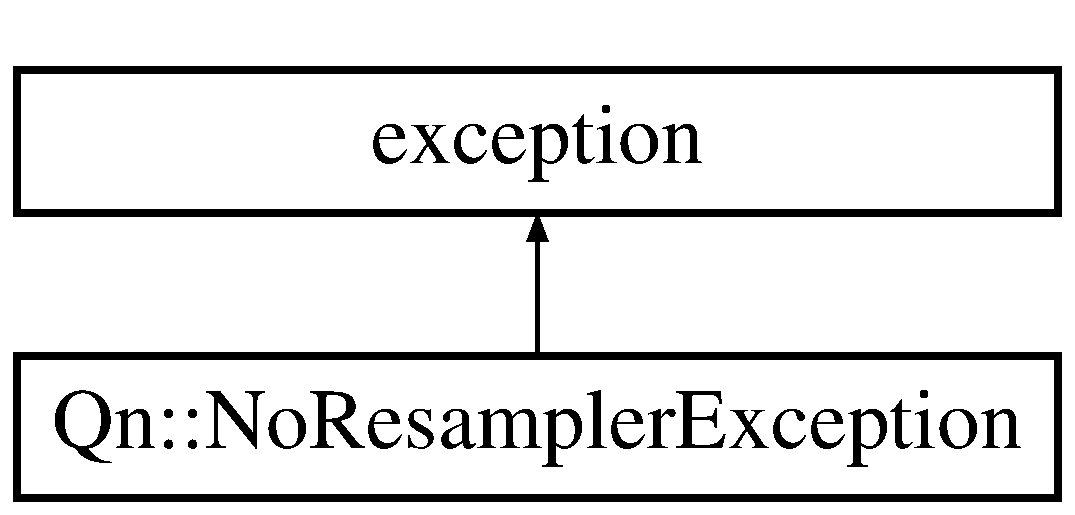
\includegraphics[height=2.000000cm]{structQn_1_1NoResamplerException}
\end{center}
\end{figure}
\subsection*{Public Member Functions}
\begin{DoxyCompactItemize}
\item 
\mbox{\Hypertarget{structQn_1_1NoResamplerException_a4bac2d2e5129e8ce0bbb17c582589bed}\label{structQn_1_1NoResamplerException_a4bac2d2e5129e8ce0bbb17c582589bed}} 
const char $\ast$ {\bfseries what} () const noexcept override
\end{DoxyCompactItemize}


The documentation for this struct was generated from the following file\+:\begin{DoxyCompactItemize}
\item 
D\+T\+\_\+\+Flow/\+Correlation/include/Stats\+Result.\+h\end{DoxyCompactItemize}

\hypertarget{classOutValue}{}\section{Out\+Value$<$ T $>$ Class Template Reference}
\label{classOutValue}\index{Out\+Value$<$ T $>$@{Out\+Value$<$ T $>$}}


Attaches a variable to a chosen tree. Type is converted to the chosen type.  




{\ttfamily \#include $<$Variable\+Manager.\+h$>$}

\subsection*{Public Member Functions}
\begin{DoxyCompactItemize}
\item 
\mbox{\Hypertarget{classOutValue_a800a48d36f71a786ca7a63a1391efd1b}\label{classOutValue_a800a48d36f71a786ca7a63a1391efd1b}} 
{\bfseries Out\+Value} (\mbox{\hyperlink{classQn_1_1Variable}{Qn\+::\+Variable}} var)
\item 
\mbox{\Hypertarget{classOutValue_a86be432e41b39939e9bc31719a6180a8}\label{classOutValue_a86be432e41b39939e9bc31719a6180a8}} 
void \mbox{\hyperlink{classOutValue_a86be432e41b39939e9bc31719a6180a8}{Update\+Value}} ()
\begin{DoxyCompactList}\small\item\em updates the value. To be called every event. \end{DoxyCompactList}\item 
void \mbox{\hyperlink{classOutValue_a33ee7e5f1148debbdaa83abfa1c78379}{Set\+To\+Tree}} (T\+Tree $\ast$tree)
\begin{DoxyCompactList}\small\item\em Creates a new branch in the tree. \end{DoxyCompactList}\end{DoxyCompactItemize}


\subsection{Detailed Description}
\subsubsection*{template$<$typename T$>$\newline
class Out\+Value$<$ T $>$}

Attaches a variable to a chosen tree. Type is converted to the chosen type. 


\begin{DoxyTemplParams}{Template Parameters}
{\em T} & type of variable saved in the tree. \\
\hline
\end{DoxyTemplParams}


\subsection{Member Function Documentation}
\mbox{\Hypertarget{classOutValue_a33ee7e5f1148debbdaa83abfa1c78379}\label{classOutValue_a33ee7e5f1148debbdaa83abfa1c78379}} 
\index{Out\+Value@{Out\+Value}!Set\+To\+Tree@{Set\+To\+Tree}}
\index{Set\+To\+Tree@{Set\+To\+Tree}!Out\+Value@{Out\+Value}}
\subsubsection{\texorpdfstring{Set\+To\+Tree()}{SetToTree()}}
{\footnotesize\ttfamily template$<$typename T$>$ \\
void \mbox{\hyperlink{classOutValue}{Out\+Value}}$<$ T $>$\+::Set\+To\+Tree (\begin{DoxyParamCaption}\item[{T\+Tree $\ast$}]{tree }\end{DoxyParamCaption})\hspace{0.3cm}{\ttfamily [inline]}}



Creates a new branch in the tree. 


\begin{DoxyParams}{Parameters}
{\em tree} & output tree \\
\hline
\end{DoxyParams}


The documentation for this class was generated from the following file\+:\begin{DoxyCompactItemize}
\item 
D\+T\+\_\+\+Flow/\+Correction/include/Variable\+Manager.\+h\end{DoxyCompactItemize}

\hypertarget{structQn_1_1Product}{}\section{Qn\+:\+:Product Struct Reference}
\label{structQn_1_1Product}\index{Qn\+::\+Product@{Qn\+::\+Product}}
\subsection*{Public Member Functions}
\begin{DoxyCompactItemize}
\item 
\mbox{\Hypertarget{structQn_1_1Product_a6b1e4f575d62b58247b0188256815663}\label{structQn_1_1Product_a6b1e4f575d62b58247b0188256815663}} 
{\bfseries Product} (double result, bool valid, double inweight)
\end{DoxyCompactItemize}
\subsection*{Public Attributes}
\begin{DoxyCompactItemize}
\item 
\mbox{\Hypertarget{structQn_1_1Product_ae0264d0cb7cc15f3acd10d7475ef43fa}\label{structQn_1_1Product_ae0264d0cb7cc15f3acd10d7475ef43fa}} 
double {\bfseries result} = 0.
\item 
\mbox{\Hypertarget{structQn_1_1Product_ae7f162e1fba2cf8ba29d407ac7ed01ae}\label{structQn_1_1Product_ae7f162e1fba2cf8ba29d407ac7ed01ae}} 
bool \mbox{\hyperlink{structQn_1_1Product_ae7f162e1fba2cf8ba29d407ac7ed01ae}{validity}} = false
\begin{DoxyCompactList}\small\item\em !$<$! value of the product \end{DoxyCompactList}\item 
\mbox{\Hypertarget{structQn_1_1Product_a95ed75911974232fdfe1a8a648d89bdc}\label{structQn_1_1Product_a95ed75911974232fdfe1a8a648d89bdc}} 
double \mbox{\hyperlink{structQn_1_1Product_a95ed75911974232fdfe1a8a648d89bdc}{weight}} = 1.
\begin{DoxyCompactList}\small\item\em !$<$! flag to show if product is valid \end{DoxyCompactList}\end{DoxyCompactItemize}


The documentation for this struct was generated from the following file\+:\begin{DoxyCompactItemize}
\item 
D\+T\+\_\+\+Flow/\+Base/include/Product.\+h\end{DoxyCompactItemize}

\hypertarget{classQn_1_1Profile}{}\section{Qn\+:\+:Profile Class Reference}
\label{classQn_1_1Profile}\index{Qn\+::\+Profile@{Qn\+::\+Profile}}
\subsection*{Public Member Functions}
\begin{DoxyCompactItemize}
\item 
\mbox{\Hypertarget{classQn_1_1Profile_a923d60063e1146e1ba3efa2780fa6e13}\label{classQn_1_1Profile_a923d60063e1146e1ba3efa2780fa6e13}} 
void {\bfseries Fill} (const \mbox{\hyperlink{structQn_1_1Product}{Product}} \&prod)
\item 
\mbox{\Hypertarget{classQn_1_1Profile_a3f7de0baedd56363aff0371ca2ff7ef3}\label{classQn_1_1Profile_a3f7de0baedd56363aff0371ca2ff7ef3}} 
void {\bfseries Fill} (const double result, const double weight)
\item 
\mbox{\Hypertarget{classQn_1_1Profile_ae4de768e843b7057ca505afdf399cdc0}\label{classQn_1_1Profile_ae4de768e843b7057ca505afdf399cdc0}} 
double {\bfseries Mean} () const
\item 
\mbox{\Hypertarget{classQn_1_1Profile_af24377238e442414bb2849687e5badc7}\label{classQn_1_1Profile_af24377238e442414bb2849687e5badc7}} 
int {\bfseries Entries} () const
\item 
\mbox{\Hypertarget{classQn_1_1Profile_a605675b9e0382bee6c8d2ba12adf63f5}\label{classQn_1_1Profile_a605675b9e0382bee6c8d2ba12adf63f5}} 
double {\bfseries Sum\+Of\+Weights} () const
\item 
\mbox{\Hypertarget{classQn_1_1Profile_a36716bb08d244f28d0696f13dfff6f62}\label{classQn_1_1Profile_a36716bb08d244f28d0696f13dfff6f62}} 
double {\bfseries Error} () const
\item 
\mbox{\Hypertarget{classQn_1_1Profile_af68184508ef7feb43a36a9db78787ca5}\label{classQn_1_1Profile_af68184508ef7feb43a36a9db78787ca5}} 
void {\bfseries Calculate\+Point\+Average} ()
\item 
\mbox{\Hypertarget{classQn_1_1Profile_abfe40e0bd565f4516faf1c437efe2cfb}\label{classQn_1_1Profile_abfe40e0bd565f4516faf1c437efe2cfb}} 
double {\bfseries Mean\+PA} () const
\item 
\mbox{\Hypertarget{classQn_1_1Profile_aa3451138ba2a66e1e0977077ddfe53d5}\label{classQn_1_1Profile_aa3451138ba2a66e1e0977077ddfe53d5}} 
double {\bfseries Error\+PA} () const
\item 
\mbox{\Hypertarget{classQn_1_1Profile_a6f7e2ef76edf983d61432bf106e221ff}\label{classQn_1_1Profile_a6f7e2ef76edf983d61432bf106e221ff}} 
void {\bfseries Print} ()
\end{DoxyCompactItemize}
\subsection*{Static Public Member Functions}
\begin{DoxyCompactItemize}
\item 
\mbox{\Hypertarget{classQn_1_1Profile_a0cc0eb7446f5df2538ef2e74a23e9370}\label{classQn_1_1Profile_a0cc0eb7446f5df2538ef2e74a23e9370}} 
static \mbox{\hyperlink{classQn_1_1Profile}{Profile}} {\bfseries Merge\+Normal} (const \mbox{\hyperlink{classQn_1_1Profile}{Profile}} \&, const \mbox{\hyperlink{classQn_1_1Profile}{Profile}} \&)
\item 
\mbox{\Hypertarget{classQn_1_1Profile_a6da2a95bfcfc64778a071afe53081ff8}\label{classQn_1_1Profile_a6da2a95bfcfc64778a071afe53081ff8}} 
static \mbox{\hyperlink{classQn_1_1Profile}{Profile}} {\bfseries Merge\+Point\+Average} (const \mbox{\hyperlink{classQn_1_1Profile}{Profile}} \&, const \mbox{\hyperlink{classQn_1_1Profile}{Profile}} \&)
\item 
\mbox{\Hypertarget{classQn_1_1Profile_a4b0d9721247f1b92eff359d1a08b7f89}\label{classQn_1_1Profile_a4b0d9721247f1b92eff359d1a08b7f89}} 
static \mbox{\hyperlink{classQn_1_1Profile}{Profile}} {\bfseries Addition\+Normal} (const \mbox{\hyperlink{classQn_1_1Profile}{Profile}} \&, const \mbox{\hyperlink{classQn_1_1Profile}{Profile}} \&)
\item 
\mbox{\Hypertarget{classQn_1_1Profile_adad2e4666f8105b1db929f638928640e}\label{classQn_1_1Profile_adad2e4666f8105b1db929f638928640e}} 
static \mbox{\hyperlink{classQn_1_1Profile}{Profile}} {\bfseries Addition\+Point\+Average} (const \mbox{\hyperlink{classQn_1_1Profile}{Profile}} \&, const \mbox{\hyperlink{classQn_1_1Profile}{Profile}} \&)
\item 
\mbox{\Hypertarget{classQn_1_1Profile_ad63be60ee11c31fc9c3bc65978f7447a}\label{classQn_1_1Profile_ad63be60ee11c31fc9c3bc65978f7447a}} 
static \mbox{\hyperlink{classQn_1_1Profile}{Profile}} {\bfseries Subtraction\+Normal} (const \mbox{\hyperlink{classQn_1_1Profile}{Profile}} \&, const \mbox{\hyperlink{classQn_1_1Profile}{Profile}} \&)
\item 
\mbox{\Hypertarget{classQn_1_1Profile_a612cff844bf93f356ac28c08f0b5910b}\label{classQn_1_1Profile_a612cff844bf93f356ac28c08f0b5910b}} 
static \mbox{\hyperlink{classQn_1_1Profile}{Profile}} {\bfseries Subtraction\+Point\+Average} (const \mbox{\hyperlink{classQn_1_1Profile}{Profile}} \&, const \mbox{\hyperlink{classQn_1_1Profile}{Profile}} \&)
\item 
\mbox{\Hypertarget{classQn_1_1Profile_a744c728a961b0c5fa4aeb28a5b1d4c58}\label{classQn_1_1Profile_a744c728a961b0c5fa4aeb28a5b1d4c58}} 
static \mbox{\hyperlink{classQn_1_1Profile}{Profile}} {\bfseries Multiplication\+Normal} (const \mbox{\hyperlink{classQn_1_1Profile}{Profile}} \&, const \mbox{\hyperlink{classQn_1_1Profile}{Profile}} \&)
\item 
\mbox{\Hypertarget{classQn_1_1Profile_a640d37308b7b1dc10d5a9343ffa64049}\label{classQn_1_1Profile_a640d37308b7b1dc10d5a9343ffa64049}} 
static \mbox{\hyperlink{classQn_1_1Profile}{Profile}} {\bfseries Multiplication\+Point\+Average} (const \mbox{\hyperlink{classQn_1_1Profile}{Profile}} \&, const \mbox{\hyperlink{classQn_1_1Profile}{Profile}} \&)
\item 
\mbox{\Hypertarget{classQn_1_1Profile_a1226ec6d8284da2da7e03fd40e7e45bb}\label{classQn_1_1Profile_a1226ec6d8284da2da7e03fd40e7e45bb}} 
static \mbox{\hyperlink{classQn_1_1Profile}{Profile}} {\bfseries Division\+Normal} (const \mbox{\hyperlink{classQn_1_1Profile}{Profile}} \&, const \mbox{\hyperlink{classQn_1_1Profile}{Profile}} \&)
\item 
\mbox{\Hypertarget{classQn_1_1Profile_a19066a004019297ef7c60ec1d93cea76}\label{classQn_1_1Profile_a19066a004019297ef7c60ec1d93cea76}} 
static \mbox{\hyperlink{classQn_1_1Profile}{Profile}} {\bfseries Division\+Point\+Average} (const \mbox{\hyperlink{classQn_1_1Profile}{Profile}} \&, const \mbox{\hyperlink{classQn_1_1Profile}{Profile}} \&)
\item 
\mbox{\Hypertarget{classQn_1_1Profile_a66cfc60e61cc7c32c5e7b6028e0ce9f3}\label{classQn_1_1Profile_a66cfc60e61cc7c32c5e7b6028e0ce9f3}} 
static \mbox{\hyperlink{classQn_1_1Profile}{Profile}} {\bfseries Sqrt\+Normal} (const \mbox{\hyperlink{classQn_1_1Profile}{Profile}} \&)
\item 
\mbox{\Hypertarget{classQn_1_1Profile_add15aa3e9c72e4dc590f9a95383e2fe5}\label{classQn_1_1Profile_add15aa3e9c72e4dc590f9a95383e2fe5}} 
static \mbox{\hyperlink{classQn_1_1Profile}{Profile}} {\bfseries Sqrt\+Point\+Average} (const \mbox{\hyperlink{classQn_1_1Profile}{Profile}} \&)
\item 
\mbox{\Hypertarget{classQn_1_1Profile_ada03e1affd51e7e22e40ea73eeb2ce3d}\label{classQn_1_1Profile_ada03e1affd51e7e22e40ea73eeb2ce3d}} 
static \mbox{\hyperlink{classQn_1_1Profile}{Profile}} {\bfseries Scale\+Normal} (const \mbox{\hyperlink{classQn_1_1Profile}{Profile}} \&, double)
\item 
\mbox{\Hypertarget{classQn_1_1Profile_a5374855e471f2dd35c2060249e48f684}\label{classQn_1_1Profile_a5374855e471f2dd35c2060249e48f684}} 
static \mbox{\hyperlink{classQn_1_1Profile}{Profile}} {\bfseries Scale\+Point\+Average} (const \mbox{\hyperlink{classQn_1_1Profile}{Profile}} \&, double)
\end{DoxyCompactItemize}


The documentation for this class was generated from the following files\+:\begin{DoxyCompactItemize}
\item 
D\+T\+\_\+\+Flow/\+Base/include/Profile.\+h\item 
D\+T\+\_\+\+Flow/\+Base/Profile.\+cpp\end{DoxyCompactItemize}

\hypertarget{structQn_1_1Internal_1_1ProjectionDrawable}{}\section{Qn\+:\+:Internal\+:\+:Projection\+Drawable$<$ T $>$ Struct Template Reference}
\label{structQn_1_1Internal_1_1ProjectionDrawable}\index{Qn\+::\+Internal\+::\+Projection\+Drawable$<$ T $>$@{Qn\+::\+Internal\+::\+Projection\+Drawable$<$ T $>$}}


Template class to facilitate the drawing of Projections of \mbox{\hyperlink{classQn_1_1DataContainer}{Data\+Container}}.  




{\ttfamily \#include $<$Data\+Container\+Helper.\+h$>$}

Inheritance diagram for Qn\+:\+:Internal\+:\+:Projection\+Drawable$<$ T $>$\+:\begin{figure}[H]
\begin{center}
\leavevmode
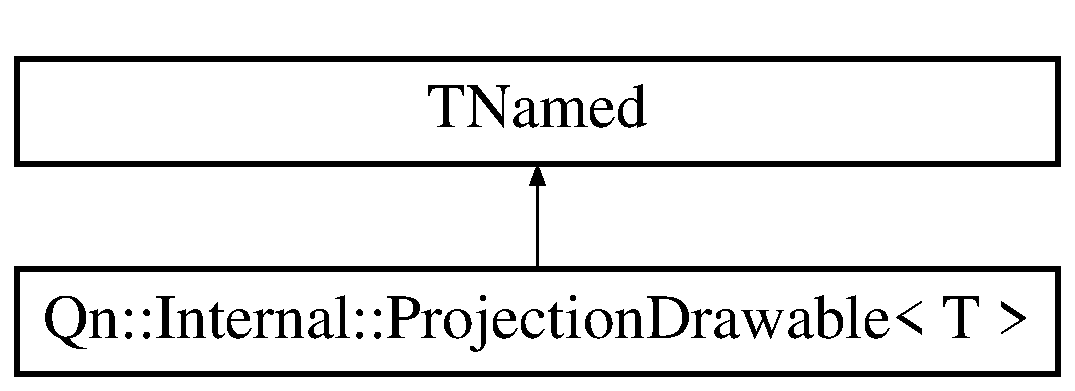
\includegraphics[height=2.000000cm]{structQn_1_1Internal_1_1ProjectionDrawable}
\end{center}
\end{figure}
\subsection*{Public Member Functions}
\begin{DoxyCompactItemize}
\item 
\mbox{\Hypertarget{structQn_1_1Internal_1_1ProjectionDrawable_a692fe39c9a74d689cc4679a190559805}\label{structQn_1_1Internal_1_1ProjectionDrawable_a692fe39c9a74d689cc4679a190559805}} 
{\bfseries Projection\+Drawable} (T projection)
\item 
\mbox{\Hypertarget{structQn_1_1Internal_1_1ProjectionDrawable_adb1b914219cad6cd49e8a35e8781be4a}\label{structQn_1_1Internal_1_1ProjectionDrawable_adb1b914219cad6cd49e8a35e8781be4a}} 
void {\bfseries Browse} (T\+Browser $\ast$b) override
\end{DoxyCompactItemize}
\subsection*{Public Attributes}
\begin{DoxyCompactItemize}
\item 
\mbox{\Hypertarget{structQn_1_1Internal_1_1ProjectionDrawable_aef9fa3539e77e695d40c658048e1faf4}\label{structQn_1_1Internal_1_1ProjectionDrawable_aef9fa3539e77e695d40c658048e1faf4}} 
T {\bfseries graph} = nullptr
\end{DoxyCompactItemize}


\subsection{Detailed Description}
\subsubsection*{template$<$typename T$>$\newline
struct Qn\+::\+Internal\+::\+Projection\+Drawable$<$ T $>$}

Template class to facilitate the drawing of Projections of \mbox{\hyperlink{classQn_1_1DataContainer}{Data\+Container}}. 

\begin{DoxyAttention}{Attention}
Takes ownership of graph and will delete it at the end of the lifetime. 
\end{DoxyAttention}

\begin{DoxyTemplParams}{Template Parameters}
{\em T} & Type of Graph to draw. \\
\hline
\end{DoxyTemplParams}


The documentation for this struct was generated from the following file\+:\begin{DoxyCompactItemize}
\item 
D\+T\+\_\+\+Flow/\+Base/include/Data\+Container\+Helper.\+h\end{DoxyCompactItemize}

\hypertarget{classQn_1_1QAHisto}{}\section{Qn\+:\+:Q\+A\+Histo$<$ H\+I\+S\+TO, N, V\+AR $>$ Class Template Reference}
\label{classQn_1_1QAHisto}\index{Qn\+::\+Q\+A\+Histo$<$ H\+I\+S\+T\+O, N, V\+A\+R $>$@{Qn\+::\+Q\+A\+Histo$<$ H\+I\+S\+T\+O, N, V\+A\+R $>$}}


{\ttfamily \#include $<$Q\+A\+Histogram.\+h$>$}

Inheritance diagram for Qn\+:\+:Q\+A\+Histo$<$ H\+I\+S\+TO, N, V\+AR $>$\+:\begin{figure}[H]
\begin{center}
\leavevmode
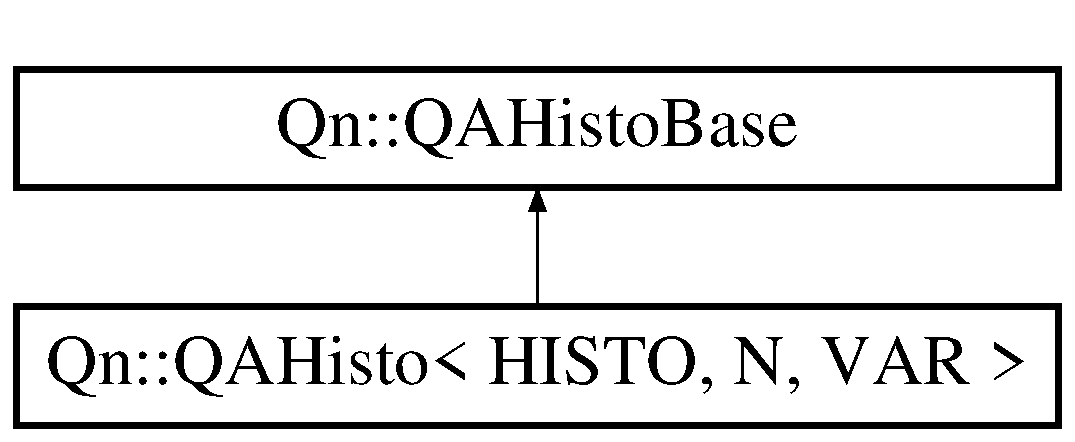
\includegraphics[height=2.000000cm]{classQn_1_1QAHisto}
\end{center}
\end{figure}
\subsection*{Public Member Functions}
\begin{DoxyCompactItemize}
\item 
\mbox{\Hypertarget{classQn_1_1QAHisto_a3bec5933f9d3ecc7f30d508d236ffd30}\label{classQn_1_1QAHisto_a3bec5933f9d3ecc7f30d508d236ffd30}} 
{\bfseries Q\+A\+Histo} (std\+::array$<$ V\+AR, N $>$ vec, H\+I\+S\+TO histo, std\+::unique\+\_\+ptr$<$ \mbox{\hyperlink{classQn_1_1Axis}{Qn\+::\+Axis}} $>$ axis, \mbox{\hyperlink{classQn_1_1Variable}{Qn\+::\+Variable}} axisvar)
\item 
\mbox{\Hypertarget{classQn_1_1QAHisto_ac6e9d11cf5550b8915419f8821616078}\label{classQn_1_1QAHisto_ac6e9d11cf5550b8915419f8821616078}} 
{\bfseries Q\+A\+Histo} (std\+::array$<$ V\+AR, N $>$ vec, H\+I\+S\+TO histo)
\item 
{\footnotesize template$<$typename array , std\+::size\+\_\+t... I$>$ }\\void \mbox{\hyperlink{classQn_1_1QAHisto_a2cf01f7749c505bdbc14a0895c06d41a}{Fill\+Impl}} (const array a, std\+::index\+\_\+sequence$<$ I... $>$)
\item 
void \mbox{\hyperlink{classQn_1_1QAHisto_a0841ac824d99d03b4f2646b62bf9c93e}{Fill}} () override
\item 
void \mbox{\hyperlink{classQn_1_1QAHisto_a3d5c6dde0416609c37bfc847955e0b8d}{Add\+To\+List}} (T\+List $\ast$list) override
\end{DoxyCompactItemize}


\subsection{Detailed Description}
\subsubsection*{template$<$typename H\+I\+S\+TO, int N, typename V\+AR$>$\newline
class Qn\+::\+Q\+A\+Histo$<$ H\+I\+S\+T\+O, N, V\+A\+R $>$}

Wrapper for a R\+O\+OT histogram, which allows it to be filled by the correction manager. 
\begin{DoxyTemplParams}{Template Parameters}
{\em H\+I\+S\+TO} & type of histogram. \\
\hline
{\em N} & number of dimensions \\
\hline
{\em V\+AR} & Type of the variable \\
\hline
\end{DoxyTemplParams}


\subsection{Member Function Documentation}
\mbox{\Hypertarget{classQn_1_1QAHisto_a3d5c6dde0416609c37bfc847955e0b8d}\label{classQn_1_1QAHisto_a3d5c6dde0416609c37bfc847955e0b8d}} 
\index{Qn\+::\+Q\+A\+Histo@{Qn\+::\+Q\+A\+Histo}!Add\+To\+List@{Add\+To\+List}}
\index{Add\+To\+List@{Add\+To\+List}!Qn\+::\+Q\+A\+Histo@{Qn\+::\+Q\+A\+Histo}}
\subsubsection{\texorpdfstring{Add\+To\+List()}{AddToList()}}
{\footnotesize\ttfamily template$<$typename H\+I\+S\+TO , int N, typename V\+AR $>$ \\
void \mbox{\hyperlink{classQn_1_1QAHisto}{Qn\+::\+Q\+A\+Histo}}$<$ H\+I\+S\+TO, N, V\+AR $>$\+::Add\+To\+List (\begin{DoxyParamCaption}\item[{T\+List $\ast$}]{list }\end{DoxyParamCaption})\hspace{0.3cm}{\ttfamily [inline]}, {\ttfamily [override]}, {\ttfamily [virtual]}}

Add the histogram to the list. 
\begin{DoxyParams}{Parameters}
{\em list} & pointer to the list. Lifetime of the histogram hast to be managed by the list. \\
\hline
\end{DoxyParams}


Implements \mbox{\hyperlink{structQn_1_1QAHistoBase}{Qn\+::\+Q\+A\+Histo\+Base}}.

\mbox{\Hypertarget{classQn_1_1QAHisto_a0841ac824d99d03b4f2646b62bf9c93e}\label{classQn_1_1QAHisto_a0841ac824d99d03b4f2646b62bf9c93e}} 
\index{Qn\+::\+Q\+A\+Histo@{Qn\+::\+Q\+A\+Histo}!Fill@{Fill}}
\index{Fill@{Fill}!Qn\+::\+Q\+A\+Histo@{Qn\+::\+Q\+A\+Histo}}
\subsubsection{\texorpdfstring{Fill()}{Fill()}}
{\footnotesize\ttfamily template$<$typename H\+I\+S\+TO , int N, typename V\+AR $>$ \\
void \mbox{\hyperlink{classQn_1_1QAHisto}{Qn\+::\+Q\+A\+Histo}}$<$ H\+I\+S\+TO, N, V\+AR $>$\+::Fill (\begin{DoxyParamCaption}{ }\end{DoxyParamCaption})\hspace{0.3cm}{\ttfamily [inline]}, {\ttfamily [override]}, {\ttfamily [virtual]}}

Fill function. 

Implements \mbox{\hyperlink{structQn_1_1QAHistoBase}{Qn\+::\+Q\+A\+Histo\+Base}}.

\mbox{\Hypertarget{classQn_1_1QAHisto_a2cf01f7749c505bdbc14a0895c06d41a}\label{classQn_1_1QAHisto_a2cf01f7749c505bdbc14a0895c06d41a}} 
\index{Qn\+::\+Q\+A\+Histo@{Qn\+::\+Q\+A\+Histo}!Fill\+Impl@{Fill\+Impl}}
\index{Fill\+Impl@{Fill\+Impl}!Qn\+::\+Q\+A\+Histo@{Qn\+::\+Q\+A\+Histo}}
\subsubsection{\texorpdfstring{Fill\+Impl()}{FillImpl()}}
{\footnotesize\ttfamily template$<$typename H\+I\+S\+TO , int N, typename V\+AR $>$ \\
template$<$typename array , std\+::size\+\_\+t... I$>$ \\
void \mbox{\hyperlink{classQn_1_1QAHisto}{Qn\+::\+Q\+A\+Histo}}$<$ H\+I\+S\+TO, N, V\+AR $>$\+::Fill\+Impl (\begin{DoxyParamCaption}\item[{const array}]{a,  }\item[{std\+::index\+\_\+sequence$<$ I... $>$}]{ }\end{DoxyParamCaption})\hspace{0.3cm}{\ttfamily [inline]}}

Implementation of the fill function 
\begin{DoxyTemplParams}{Template Parameters}
{\em array} & type of array \\
\hline
{\em I} & index sequence \\
\hline
\end{DoxyTemplParams}

\begin{DoxyParams}{Parameters}
{\em a} & Array of variables used for filling the histogram \\
\hline
\end{DoxyParams}


The documentation for this class was generated from the following file\+:\begin{DoxyCompactItemize}
\item 
D\+T\+\_\+\+Flow/\+Correction/include/Q\+A\+Histogram.\+h\end{DoxyCompactItemize}

\hypertarget{structQn_1_1QAHistoBase}{}\section{Qn\+:\+:Q\+A\+Histo\+Base Struct Reference}
\label{structQn_1_1QAHistoBase}\index{Qn\+::\+Q\+A\+Histo\+Base@{Qn\+::\+Q\+A\+Histo\+Base}}


{\ttfamily \#include $<$Q\+A\+Histogram.\+h$>$}

Inheritance diagram for Qn\+:\+:Q\+A\+Histo\+Base\+:\begin{figure}[H]
\begin{center}
\leavevmode
\includegraphics[height=2.000000cm]{structQn_1_1QAHistoBase}
\end{center}
\end{figure}
\subsection*{Public Member Functions}
\begin{DoxyCompactItemize}
\item 
\mbox{\Hypertarget{structQn_1_1QAHistoBase_aaa08c6aaf1756d3ff1131991bd49e655}\label{structQn_1_1QAHistoBase_aaa08c6aaf1756d3ff1131991bd49e655}} 
virtual void {\bfseries Fill} ()=0
\item 
\mbox{\Hypertarget{structQn_1_1QAHistoBase_a75180c45e0016b36c993af7677aaab12}\label{structQn_1_1QAHistoBase_a75180c45e0016b36c993af7677aaab12}} 
virtual void {\bfseries Add\+To\+List} (T\+List $\ast$)=0
\end{DoxyCompactItemize}


\subsection{Detailed Description}
\mbox{\hyperlink{classBase}{Base}} class of a QA histogram 

The documentation for this struct was generated from the following file\+:\begin{DoxyCompactItemize}
\item 
D\+T\+\_\+\+Flow/\+Correction/include/Q\+A\+Histogram.\+h\end{DoxyCompactItemize}

\hypertarget{classQnCorrectionsCorrectionOnInputData}{}\section{Qn\+Corrections\+Correction\+On\+Input\+Data Class Reference}
\label{classQnCorrectionsCorrectionOnInputData}\index{Qn\+Corrections\+Correction\+On\+Input\+Data@{Qn\+Corrections\+Correction\+On\+Input\+Data}}


\mbox{\hyperlink{classBase}{Base}} class for correction steps applied to input data.  




{\ttfamily \#include $<$Correction\+On\+Input\+Data.\+h$>$}



\subsection{Detailed Description}
\mbox{\hyperlink{classBase}{Base}} class for correction steps applied to input data. 

\begin{DoxyAuthor}{Author}
Jaap Onderwaater \href{mailto:jacobus.onderwaater@cern.ch}{\tt jacobus.\+onderwaater@cern.\+ch}, G\+SI 

Ilya Selyuzhenkov \href{mailto:ilya.selyuzhenkov@gmail.com}{\tt ilya.\+selyuzhenkov@gmail.\+com}, G\+SI 

Víctor González \href{mailto:victor.gonzalez@cern.ch}{\tt victor.\+gonzalez@cern.\+ch}, U\+CM 
\end{DoxyAuthor}
\begin{DoxyDate}{Date}
Feb 05, 2016 
\end{DoxyDate}


The documentation for this class was generated from the following file\+:\begin{DoxyCompactItemize}
\item 
D\+T\+\_\+\+Flow/\+Qn\+Corrections/include/Correction\+On\+Input\+Data.\+h\end{DoxyCompactItemize}

\hypertarget{classQnCorrectionsCorrectionOnQvector}{}\section{Qn\+Corrections\+Correction\+On\+Qvector Class Reference}
\label{classQnCorrectionsCorrectionOnQvector}\index{Qn\+Corrections\+Correction\+On\+Qvector@{Qn\+Corrections\+Correction\+On\+Qvector}}


\mbox{\hyperlink{classBase}{Base}} class for correction steps applied to a Q vector.  




{\ttfamily \#include $<$Correction\+On\+Qvector.\+h$>$}



\subsection{Detailed Description}
\mbox{\hyperlink{classBase}{Base}} class for correction steps applied to a Q vector. 

\begin{DoxyAuthor}{Author}
Jaap Onderwaater \href{mailto:jacobus.onderwaater@cern.ch}{\tt jacobus.\+onderwaater@cern.\+ch}, G\+SI 

Ilya Selyuzhenkov \href{mailto:ilya.selyuzhenkov@gmail.com}{\tt ilya.\+selyuzhenkov@gmail.\+com}, G\+SI 

Víctor González \href{mailto:victor.gonzalez@cern.ch}{\tt victor.\+gonzalez@cern.\+ch}, U\+CM 
\end{DoxyAuthor}
\begin{DoxyDate}{Date}
Feb 05, 2016 
\end{DoxyDate}


The documentation for this class was generated from the following file\+:\begin{DoxyCompactItemize}
\item 
D\+T\+\_\+\+Flow/\+Qn\+Corrections/include/Correction\+On\+Qvector.\+h\end{DoxyCompactItemize}

\hypertarget{classQnCorrectionsCorrectionsSetOnInputData}{}\section{Qn\+Corrections\+Corrections\+Set\+On\+Input\+Data Class Reference}
\label{classQnCorrectionsCorrectionsSetOnInputData}\index{Qn\+Corrections\+Corrections\+Set\+On\+Input\+Data@{Qn\+Corrections\+Corrections\+Set\+On\+Input\+Data}}


Encapsulate the set of corrections over input data.  




{\ttfamily \#include $<$Corrections\+Set\+On\+Input\+Data.\+h$>$}



\subsection{Detailed Description}
Encapsulate the set of corrections over input data. 

Order matters so, the list must be built with the order in which corrections should be applied.

The correction steps are own by the object instance so they will be destroyed with it.

\begin{DoxyAuthor}{Author}
Jaap Onderwaater \href{mailto:jacobus.onderwaater@cern.ch}{\tt jacobus.\+onderwaater@cern.\+ch}, G\+SI 

Ilya Selyuzhenkov \href{mailto:ilya.selyuzhenkov@gmail.com}{\tt ilya.\+selyuzhenkov@gmail.\+com}, G\+SI 

Víctor González \href{mailto:victor.gonzalez@cern.ch}{\tt victor.\+gonzalez@cern.\+ch}, U\+CM 
\end{DoxyAuthor}
\begin{DoxyDate}{Date}
Feb 05, 2016 
\end{DoxyDate}


The documentation for this class was generated from the following file\+:\begin{DoxyCompactItemize}
\item 
D\+T\+\_\+\+Flow/\+Qn\+Corrections/include/Corrections\+Set\+On\+Input\+Data.\+h\end{DoxyCompactItemize}

\hypertarget{classQnCorrectionsCorrectionsSetOnQvector}{}\section{Qn\+Corrections\+Corrections\+Set\+On\+Qvector Class Reference}
\label{classQnCorrectionsCorrectionsSetOnQvector}\index{Qn\+Corrections\+Corrections\+Set\+On\+Qvector@{Qn\+Corrections\+Corrections\+Set\+On\+Qvector}}


Encapsulate the set of corrections to apply on Q vectors.  




{\ttfamily \#include $<$Corrections\+Set\+On\+Qvector.\+h$>$}



\subsection{Detailed Description}
Encapsulate the set of corrections to apply on Q vectors. 

Order matters so, the list must be built with the order in which corrections should be applied.

The correction steps are own by the object instance so they will be destroyed with it.

\begin{DoxyAuthor}{Author}
Jaap Onderwaater \href{mailto:jacobus.onderwaater@cern.ch}{\tt jacobus.\+onderwaater@cern.\+ch}, G\+SI 

Ilya Selyuzhenkov \href{mailto:ilya.selyuzhenkov@gmail.com}{\tt ilya.\+selyuzhenkov@gmail.\+com}, G\+SI 

Víctor González \href{mailto:victor.gonzalez@cern.ch}{\tt victor.\+gonzalez@cern.\+ch}, U\+CM 
\end{DoxyAuthor}
\begin{DoxyDate}{Date}
Feb 05, 2016 
\end{DoxyDate}


The documentation for this class was generated from the following file\+:\begin{DoxyCompactItemize}
\item 
D\+T\+\_\+\+Flow/\+Qn\+Corrections/include/Corrections\+Set\+On\+Qvector.\+h\end{DoxyCompactItemize}

\hypertarget{classQnCorrectionsCorrectionStepBase}{}\section{Qn\+Corrections\+Correction\+Step\+Base Class Reference}
\label{classQnCorrectionsCorrectionStepBase}\index{Qn\+Corrections\+Correction\+Step\+Base@{Qn\+Corrections\+Correction\+Step\+Base}}


\mbox{\hyperlink{classBase}{Base}} class for correction steps.  




{\ttfamily \#include $<$Correction\+Step\+Base.\+h$>$}



\subsection{Detailed Description}
\mbox{\hyperlink{classBase}{Base}} class for correction steps. 

Each correction has a name and a key. The name identifies it in an open way while the key is used to codify its position in an ordered list of consecutive corrections.

\begin{DoxyAuthor}{Author}
Jaap Onderwaater \href{mailto:jacobus.onderwaater@cern.ch}{\tt jacobus.\+onderwaater@cern.\+ch}, G\+SI 

Ilya Selyuzhenkov \href{mailto:ilya.selyuzhenkov@gmail.com}{\tt ilya.\+selyuzhenkov@gmail.\+com}, G\+SI 

Víctor González \href{mailto:victor.gonzalez@cern.ch}{\tt victor.\+gonzalez@cern.\+ch}, U\+CM 
\end{DoxyAuthor}
\begin{DoxyDate}{Date}
Feb 05, 2016 
\end{DoxyDate}


The documentation for this class was generated from the following file\+:\begin{DoxyCompactItemize}
\item 
D\+T\+\_\+\+Flow/\+Qn\+Corrections/include/Correction\+Step\+Base.\+h\end{DoxyCompactItemize}

\hypertarget{classQnCorrectionsCutAbove}{}\section{Qn\+Corrections\+Cut\+Above Class Reference}
\label{classQnCorrectionsCutAbove}\index{Qn\+Corrections\+Cut\+Above@{Qn\+Corrections\+Cut\+Above}}


Lower limit cut class for Q vector correction.  




{\ttfamily \#include $<$Cut\+Above.\+h$>$}



\subsection{Detailed Description}
Lower limit cut class for Q vector correction. 

Provides support for cuts based in a lower limit

Stores the threshold value and pass the var Id to its parent. Implements Is\+Selected accordingly.

\begin{DoxyAuthor}{Author}
Jaap Onderwaater \href{mailto:jacobus.onderwaater@cern.ch}{\tt jacobus.\+onderwaater@cern.\+ch}, G\+SI 

Ilya Selyuzhenkov \href{mailto:ilya.selyuzhenkov@gmail.com}{\tt ilya.\+selyuzhenkov@gmail.\+com}, G\+SI 

Víctor González \href{mailto:victor.gonzalez@cern.ch}{\tt victor.\+gonzalez@cern.\+ch}, U\+CM 
\end{DoxyAuthor}
\begin{DoxyDate}{Date}
Jan 22, 2016 
\end{DoxyDate}


The documentation for this class was generated from the following file\+:\begin{DoxyCompactItemize}
\item 
D\+T\+\_\+\+Flow/\+Qn\+Corrections/include/Cut\+Above.\+h\end{DoxyCompactItemize}

\hypertarget{classQnCorrectionsCutBelow}{}\section{Qn\+Corrections\+Cut\+Below Class Reference}
\label{classQnCorrectionsCutBelow}\index{Qn\+Corrections\+Cut\+Below@{Qn\+Corrections\+Cut\+Below}}


Upper limit cut class for Q vector correction.  




{\ttfamily \#include $<$Cut\+Below.\+h$>$}



\subsection{Detailed Description}
Upper limit cut class for Q vector correction. 

Provides support for cuts based in an upper limit

Stores the threshold value and pass the var Id to its parent. Implements Is\+Selected accordingly.

\begin{DoxyAuthor}{Author}
Jaap Onderwaater \href{mailto:jacobus.onderwaater@cern.ch}{\tt jacobus.\+onderwaater@cern.\+ch}, G\+SI 

Ilya Selyuzhenkov \href{mailto:ilya.selyuzhenkov@gmail.com}{\tt ilya.\+selyuzhenkov@gmail.\+com}, G\+SI 

Víctor González \href{mailto:victor.gonzalez@cern.ch}{\tt victor.\+gonzalez@cern.\+ch}, U\+CM 
\end{DoxyAuthor}
\begin{DoxyDate}{Date}
Jan 22, 2016 
\end{DoxyDate}


The documentation for this class was generated from the following file\+:\begin{DoxyCompactItemize}
\item 
D\+T\+\_\+\+Flow/\+Qn\+Corrections/include/Cut\+Below.\+h\end{DoxyCompactItemize}

\hypertarget{classQnCorrectionsCutOutside}{}\section{Qn\+Corrections\+Cut\+Outside Class Reference}
\label{classQnCorrectionsCutOutside}\index{Qn\+Corrections\+Cut\+Outside@{Qn\+Corrections\+Cut\+Outside}}


Outside range cut class for Q vector correction.  




{\ttfamily \#include $<$Cut\+Outside.\+h$>$}



\subsection{Detailed Description}
Outside range cut class for Q vector correction. 

Provides support for cuts based in being outside a range defined by a minimum value and a maximum value

Stores the threshold values and pass the var Id to its parent. Implements Is\+Selected accordingly.

\begin{DoxyAuthor}{Author}
Jaap Onderwaater \href{mailto:jacobus.onderwaater@cern.ch}{\tt jacobus.\+onderwaater@cern.\+ch}, G\+SI 

Ilya Selyuzhenkov \href{mailto:ilya.selyuzhenkov@gmail.com}{\tt ilya.\+selyuzhenkov@gmail.\+com}, G\+SI 

Víctor González \href{mailto:victor.gonzalez@cern.ch}{\tt victor.\+gonzalez@cern.\+ch}, U\+CM 
\end{DoxyAuthor}
\begin{DoxyDate}{Date}
Jan 22, 2016 
\end{DoxyDate}


The documentation for this class was generated from the following file\+:\begin{DoxyCompactItemize}
\item 
D\+T\+\_\+\+Flow/\+Qn\+Corrections/include/Cut\+Outside.\+h\end{DoxyCompactItemize}

\hypertarget{classQnCorrectionsCutsBase}{}\section{Qn\+Corrections\+Cuts\+Base Class Reference}
\label{classQnCorrectionsCutsBase}\index{Qn\+Corrections\+Cuts\+Base@{Qn\+Corrections\+Cuts\+Base}}


\mbox{\hyperlink{classBase}{Base}} class for the Q vector correction cuts.  




{\ttfamily \#include $<$Cuts\+Base.\+h$>$}



\subsection{Detailed Description}
\mbox{\hyperlink{classBase}{Base}} class for the Q vector correction cuts. 

Stores the external variable Id the cut should act on

Provides the interface for the set of different cuts classes.

\begin{DoxyAuthor}{Author}
Jaap Onderwaater \href{mailto:jacobus.onderwaater@cern.ch}{\tt jacobus.\+onderwaater@cern.\+ch}, G\+SI 

Ilya Selyuzhenkov \href{mailto:ilya.selyuzhenkov@gmail.com}{\tt ilya.\+selyuzhenkov@gmail.\+com}, G\+SI 

Víctor González \href{mailto:victor.gonzalez@cern.ch}{\tt victor.\+gonzalez@cern.\+ch}, U\+CM 
\end{DoxyAuthor}
\begin{DoxyDate}{Date}
Jan 22, 2016 
\end{DoxyDate}


The documentation for this class was generated from the following file\+:\begin{DoxyCompactItemize}
\item 
D\+T\+\_\+\+Flow/\+Qn\+Corrections/include/Cuts\+Base.\+h\end{DoxyCompactItemize}

\hypertarget{classQnCorrectionsCutSetBit}{}\section{Qn\+Corrections\+Cut\+Set\+Bit Class Reference}
\label{classQnCorrectionsCutSetBit}\index{Qn\+Corrections\+Cut\+Set\+Bit@{Qn\+Corrections\+Cut\+Set\+Bit}}


Bit setting cut class for Q vector correction.  




{\ttfamily \#include $<$Cut\+Set\+Bit.\+h$>$}



\subsection{Detailed Description}
Bit setting cut class for Q vector correction. 

Provides support for cuts based in the setting or not of a concrete bit within the actual value of a variable. The selected bit is passed as an integer from 0 up to 31.

Stores the desired bit and its (un)set condition and pass the var Id to its parent. Implements Is\+Selected accordingly.

\begin{DoxyAuthor}{Author}
Jaap Onderwaater \href{mailto:jacobus.onderwaater@cern.ch}{\tt jacobus.\+onderwaater@cern.\+ch}, G\+SI 

Ilya Selyuzhenkov \href{mailto:ilya.selyuzhenkov@gmail.com}{\tt ilya.\+selyuzhenkov@gmail.\+com}, G\+SI 

Víctor González \href{mailto:victor.gonzalez@cern.ch}{\tt victor.\+gonzalez@cern.\+ch}, U\+CM 
\end{DoxyAuthor}
\begin{DoxyDate}{Date}
Jan 25, 2016 
\end{DoxyDate}


The documentation for this class was generated from the following file\+:\begin{DoxyCompactItemize}
\item 
D\+T\+\_\+\+Flow/\+Qn\+Corrections/include/Cut\+Set\+Bit.\+h\end{DoxyCompactItemize}

\hypertarget{classQnCorrectionsCutsSet}{}\section{Qn\+Corrections\+Cuts\+Set Class Reference}
\label{classQnCorrectionsCutsSet}\index{Qn\+Corrections\+Cuts\+Set@{Qn\+Corrections\+Cuts\+Set}}


Set of cuts to assign to a detector.  




{\ttfamily \#include $<$Cuts\+Set.\+h$>$}



\subsection{Detailed Description}
Set of cuts to assign to a detector. 

Array of cuts that contains the whole set of cuts to assign to a concrete detector or detector configuration to filter the desired events (in the broad sense) it will have to handle.

Inherits all the methods of T\+Obj\+Array specially the subscript \mbox{[}\mbox{]} operator and Add method that allows the array to expand.

Provides Is\+Selected that goes through the whole set of cuts to check whether the current variables values pass the them.

The cuts objects are not own by the array so, they are not destroyed when the the set is destroyed. This allows to create several sets with the same cuts. Pay attention to this when you create your cuts, they should live at least the same time you expect the sets to live.

\begin{DoxyAuthor}{Author}
Jaap Onderwaater \href{mailto:jacobus.onderwaater@cern.ch}{\tt jacobus.\+onderwaater@cern.\+ch}, G\+SI 

Ilya Selyuzhenkov \href{mailto:ilya.selyuzhenkov@gmail.com}{\tt ilya.\+selyuzhenkov@gmail.\+com}, G\+SI 

Víctor González \href{mailto:victor.gonzalez@cern.ch}{\tt victor.\+gonzalez@cern.\+ch}, U\+CM 
\end{DoxyAuthor}
\begin{DoxyDate}{Date}
Jan 4, 2016 
\end{DoxyDate}


The documentation for this class was generated from the following file\+:\begin{DoxyCompactItemize}
\item 
D\+T\+\_\+\+Flow/\+Qn\+Corrections/include/Cuts\+Set.\+h\end{DoxyCompactItemize}

\hypertarget{classQnCorrectionsCutValue}{}\section{Qn\+Corrections\+Cut\+Value Class Reference}
\label{classQnCorrectionsCutValue}\index{Qn\+Corrections\+Cut\+Value@{Qn\+Corrections\+Cut\+Value}}


Value cut class for Q vector correction.  




{\ttfamily \#include $<$Cut\+Value.\+h$>$}



\subsection{Detailed Description}
Value cut class for Q vector correction. 

Provides support for cuts based in the interest variable having a concrete value

Stores the desired value and pass the var Id to its parent. Implements Is\+Selected accordingly.

\begin{DoxyAuthor}{Author}
Jaap Onderwaater \href{mailto:jacobus.onderwaater@cern.ch}{\tt jacobus.\+onderwaater@cern.\+ch}, G\+SI 

Ilya Selyuzhenkov \href{mailto:ilya.selyuzhenkov@gmail.com}{\tt ilya.\+selyuzhenkov@gmail.\+com}, G\+SI 

Víctor González \href{mailto:victor.gonzalez@cern.ch}{\tt victor.\+gonzalez@cern.\+ch}, U\+CM 
\end{DoxyAuthor}
\begin{DoxyDate}{Date}
Jan 25, 2016 
\end{DoxyDate}


The documentation for this class was generated from the following file\+:\begin{DoxyCompactItemize}
\item 
D\+T\+\_\+\+Flow/\+Qn\+Corrections/include/Cut\+Value.\+h\end{DoxyCompactItemize}

\hypertarget{classQnCorrectionsCutWithin}{}\section{Qn\+Corrections\+Cut\+Within Class Reference}
\label{classQnCorrectionsCutWithin}\index{Qn\+Corrections\+Cut\+Within@{Qn\+Corrections\+Cut\+Within}}


Within range cut class for Q vector correction.  




{\ttfamily \#include $<$Cut\+Within.\+h$>$}



\subsection{Detailed Description}
Within range cut class for Q vector correction. 

Provides support for cuts based in being within a range defined by a minimum value and a maximum value

Stores the threshold values and pass the var Id to its parent. Implements Is\+Selected accordingly.

\begin{DoxyAuthor}{Author}
Jaap Onderwaater \href{mailto:jacobus.onderwaater@cern.ch}{\tt jacobus.\+onderwaater@cern.\+ch}, G\+SI 

Ilya Selyuzhenkov \href{mailto:ilya.selyuzhenkov@gmail.com}{\tt ilya.\+selyuzhenkov@gmail.\+com}, G\+SI 

Víctor González \href{mailto:victor.gonzalez@cern.ch}{\tt victor.\+gonzalez@cern.\+ch}, U\+CM 
\end{DoxyAuthor}
\begin{DoxyDate}{Date}
Jan 22, 2016 
\end{DoxyDate}


The documentation for this class was generated from the following file\+:\begin{DoxyCompactItemize}
\item 
D\+T\+\_\+\+Flow/\+Qn\+Corrections/include/Cut\+Within.\+h\end{DoxyCompactItemize}

\hypertarget{classQnCorrectionsDataVector}{}\section{Qn\+Corrections\+Data\+Vector Class Reference}
\label{classQnCorrectionsDataVector}\index{Qn\+Corrections\+Data\+Vector@{Qn\+Corrections\+Data\+Vector}}


Class that models and encapsulates a data vector.  




{\ttfamily \#include $<$Correction\+Data\+Vector.\+h$>$}



\subsection{Detailed Description}
Class that models and encapsulates a data vector. 

\begin{DoxyAuthor}{Author}
Jaap Onderwaater \href{mailto:jacobus.onderwaater@cern.ch}{\tt jacobus.\+onderwaater@cern.\+ch}, G\+SI 

Ilya Selyuzhenkov \href{mailto:ilya.selyuzhenkov@gmail.com}{\tt ilya.\+selyuzhenkov@gmail.\+com}, G\+SI 

Víctor González \href{mailto:victor.gonzalez@cern.ch}{\tt victor.\+gonzalez@cern.\+ch}, U\+CM 
\end{DoxyAuthor}
\begin{DoxyDate}{Date}
Feb 01, 2016 
\end{DoxyDate}


The documentation for this class was generated from the following file\+:\begin{DoxyCompactItemize}
\item 
D\+T\+\_\+\+Flow/\+Qn\+Corrections/include/Correction\+Data\+Vector.\+h\end{DoxyCompactItemize}

\hypertarget{classQnCorrectionsDataVectorChannelized}{}\section{Qn\+Corrections\+Data\+Vector\+Channelized Class Reference}
\label{classQnCorrectionsDataVectorChannelized}\index{Qn\+Corrections\+Data\+Vector\+Channelized@{Qn\+Corrections\+Data\+Vector\+Channelized}}


Data vector class from a channelized detector.  




{\ttfamily \#include $<$Correction\+Data\+Vector\+Channelized.\+h$>$}



\subsection{Detailed Description}
Data vector class from a channelized detector. 

The class expands the data vector one to incorporate channel id and two set of weights to support channel equalization procedures.

\begin{DoxyAuthor}{Author}
Jaap Onderwaater \href{mailto:jacobus.onderwaater@cern.ch}{\tt jacobus.\+onderwaater@cern.\+ch}, G\+SI 

Ilya Selyuzhenkov \href{mailto:ilya.selyuzhenkov@gmail.com}{\tt ilya.\+selyuzhenkov@gmail.\+com}, G\+SI 

Víctor González \href{mailto:victor.gonzalez@cern.ch}{\tt victor.\+gonzalez@cern.\+ch}, U\+CM 
\end{DoxyAuthor}
\begin{DoxyDate}{Date}
Jan 27, 2016 
\end{DoxyDate}


The documentation for this class was generated from the following file\+:\begin{DoxyCompactItemize}
\item 
D\+T\+\_\+\+Flow/\+Qn\+Corrections/include/Correction\+Data\+Vector\+Channelized.\+h\end{DoxyCompactItemize}

\hypertarget{classQnCorrectionsDetector}{}\section{Qn\+Corrections\+Detector Class Reference}
\label{classQnCorrectionsDetector}\index{Qn\+Corrections\+Detector@{Qn\+Corrections\+Detector}}


Detector class within Q vector correction framework.  




{\ttfamily \#include $<$Correction\+Detector.\+h$>$}



\subsection{Detailed Description}
Detector class within Q vector correction framework. 

The roles of the detector class are\+: to store its unique name and Id, and to store and handle the list of the different configurations defined for the involved detector.

The detector Id should only be obtained at creation time and the object, once created, does not allow its modification.

The detector object is in the path of the whole control flow and as such it should distribute the different commands to the defined detector configurations.

\begin{DoxyAuthor}{Author}
Jaap Onderwaater \href{mailto:jacobus.onderwaater@cern.ch}{\tt jacobus.\+onderwaater@cern.\+ch}, G\+SI 

Ilya Selyuzhenkov \href{mailto:ilya.selyuzhenkov@gmail.com}{\tt ilya.\+selyuzhenkov@gmail.\+com}, G\+SI 

Víctor González \href{mailto:victor.gonzalez@cern.ch}{\tt victor.\+gonzalez@cern.\+ch}, U\+CM 
\end{DoxyAuthor}
\begin{DoxyDate}{Date}
Feb 08, 2016 
\end{DoxyDate}


The documentation for this class was generated from the following file\+:\begin{DoxyCompactItemize}
\item 
D\+T\+\_\+\+Flow/\+Qn\+Corrections/include/Correction\+Detector.\+h\end{DoxyCompactItemize}

\hypertarget{classQnCorrectionsDetectorConfigurationBase}{}\section{Qn\+Corrections\+Detector\+Configuration\+Base Class Reference}
\label{classQnCorrectionsDetectorConfigurationBase}\index{Qn\+Corrections\+Detector\+Configuration\+Base@{Qn\+Corrections\+Detector\+Configuration\+Base}}


The base of a concrete detector configuration within Q vector correction framework.  




{\ttfamily \#include $<$Detector\+Configuration.\+h$>$}



\subsection{Detailed Description}
The base of a concrete detector configuration within Q vector correction framework. 

The detector configuration shapes a detector with a concrete set of cuts to make it the target of a Q vector correction process.

It receives the data input stream and build the corresponding Q vector associated to it for each processing request.

As such, it incorporates the set of corrections to carry on the input data and the set of corrections to perform on the produced \mbox{\hyperlink{namespaceQn}{Qn}} vector. It always stores the plain \mbox{\hyperlink{namespaceQn}{Qn}} vector produced after potential input data corrections and the \mbox{\hyperlink{namespaceQn}{Qn}} vector that incorporates the latest \mbox{\hyperlink{namespaceQn}{Qn}} vector correction step.

It also incorporates the equivalent support for Q2n vectors which could be the seed for future Q(m,n) support.

It receives at construction time the set of event classes variables and the detector reference. The reference of the detector should only be obtained at creation time and the detector configuration object, once created, does not allow its modification.

The class is a base class for further refined detector configurations.

\begin{DoxyAuthor}{Author}
Jaap Onderwaater \href{mailto:jacobus.onderwaater@cern.ch}{\tt jacobus.\+onderwaater@cern.\+ch}, G\+SI 

Ilya Selyuzhenkov \href{mailto:ilya.selyuzhenkov@gmail.com}{\tt ilya.\+selyuzhenkov@gmail.\+com}, G\+SI 

Víctor González \href{mailto:victor.gonzalez@cern.ch}{\tt victor.\+gonzalez@cern.\+ch}, U\+CM 
\end{DoxyAuthor}
\begin{DoxyDate}{Date}
Feb 08, 2016 
\end{DoxyDate}


The documentation for this class was generated from the following file\+:\begin{DoxyCompactItemize}
\item 
D\+T\+\_\+\+Flow/\+Qn\+Corrections/include/Detector\+Configuration.\+h\end{DoxyCompactItemize}

\hypertarget{classQnCorrectionsDetectorConfigurationChannels}{}\section{Qn\+Corrections\+Detector\+Configuration\+Channels Class Reference}
\label{classQnCorrectionsDetectorConfigurationChannels}\index{Qn\+Corrections\+Detector\+Configuration\+Channels@{Qn\+Corrections\+Detector\+Configuration\+Channels}}


Channel detector configuration within Q vector correction framework.  




{\ttfamily \#include $<$Detector\+Configuration\+Channels.\+h$>$}



\subsection{Detailed Description}
Channel detector configuration within Q vector correction framework. 

A channel detector within the Q vector correction framework is defined as one for which its data vectors involve azimuthal angles and channels susceptible of weighting and / or grouping and / or calibration, etc.

According to that, the proper channelized data vector is used and an extra Q vector builder is incorporated.

\begin{DoxyAuthor}{Author}
Jaap Onderwaater \href{mailto:jacobus.onderwaater@cern.ch}{\tt jacobus.\+onderwaater@cern.\+ch}, G\+SI 

Ilya Selyuzhenkov \href{mailto:ilya.selyuzhenkov@gmail.com}{\tt ilya.\+selyuzhenkov@gmail.\+com}, G\+SI 

Víctor González \href{mailto:victor.gonzalez@cern.ch}{\tt victor.\+gonzalez@cern.\+ch}, U\+CM 
\end{DoxyAuthor}
\begin{DoxyDate}{Date}
Feb 08, 2016 
\end{DoxyDate}


The documentation for this class was generated from the following file\+:\begin{DoxyCompactItemize}
\item 
D\+T\+\_\+\+Flow/\+Qn\+Corrections/include/Detector\+Configuration\+Channels.\+h\end{DoxyCompactItemize}

\hypertarget{classQnCorrectionsDetectorConfigurationsSet}{}\section{Qn\+Corrections\+Detector\+Configurations\+Set Class Reference}
\label{classQnCorrectionsDetectorConfigurationsSet}\index{Qn\+Corrections\+Detector\+Configurations\+Set@{Qn\+Corrections\+Detector\+Configurations\+Set}}


Array of detector configurations within Q vector correction framework.  




{\ttfamily \#include $<$Detector\+Configurations\+Set.\+h$>$}



\subsection{Detailed Description}
Array of detector configurations within Q vector correction framework. 

Each detector within the Q vector correction framework is able to be configured in different ways by assigning set of cuts, ordering its data within channels or even channel groups, etc. Each of these ways constitute a detector configuration. This class stores the whole set of detector configurations assigned to a concrete detector.

\begin{DoxyAuthor}{Author}
Jaap Onderwaater \href{mailto:jacobus.onderwaater@cern.ch}{\tt jacobus.\+onderwaater@cern.\+ch}, G\+SI 

Ilya Selyuzhenkov \href{mailto:ilya.selyuzhenkov@gmail.com}{\tt ilya.\+selyuzhenkov@gmail.\+com}, G\+SI 

Víctor González \href{mailto:victor.gonzalez@cern.ch}{\tt victor.\+gonzalez@cern.\+ch}, U\+CM 
\end{DoxyAuthor}
\begin{DoxyDate}{Date}
Feb 09, 2016 
\end{DoxyDate}


The documentation for this class was generated from the following file\+:\begin{DoxyCompactItemize}
\item 
D\+T\+\_\+\+Flow/\+Qn\+Corrections/include/Detector\+Configurations\+Set.\+h\end{DoxyCompactItemize}

\hypertarget{classQnCorrectionsDetectorConfigurationTracks}{}\section{Qn\+Corrections\+Detector\+Configuration\+Tracks Class Reference}
\label{classQnCorrectionsDetectorConfigurationTracks}\index{Qn\+Corrections\+Detector\+Configuration\+Tracks@{Qn\+Corrections\+Detector\+Configuration\+Tracks}}


Track detector configuration within Q vector correction framework.  




{\ttfamily \#include $<$Detector\+Configuration\+Tracks.\+h$>$}



\subsection{Detailed Description}
Track detector configuration within Q vector correction framework. 

A track detector within the Q vector correction framework is defined as one for which its data vectors only involve azimuthal angles and a potential weight. Apart from that no other input data calibration is available.

\begin{DoxyAuthor}{Author}
Jaap Onderwaater \href{mailto:jacobus.onderwaater@cern.ch}{\tt jacobus.\+onderwaater@cern.\+ch}, G\+SI 

Ilya Selyuzhenkov \href{mailto:ilya.selyuzhenkov@gmail.com}{\tt ilya.\+selyuzhenkov@gmail.\+com}, G\+SI 

Víctor González \href{mailto:victor.gonzalez@cern.ch}{\tt victor.\+gonzalez@cern.\+ch}, U\+CM 
\end{DoxyAuthor}
\begin{DoxyDate}{Date}
Feb 08, 2016 
\end{DoxyDate}


The documentation for this class was generated from the following file\+:\begin{DoxyCompactItemize}
\item 
D\+T\+\_\+\+Flow/\+Qn\+Corrections/include/Detector\+Configuration\+Tracks.\+h\end{DoxyCompactItemize}

\hypertarget{classQnCorrectionsEventClassVariable}{}\section{Qn\+Corrections\+Event\+Class\+Variable Class Reference}
\label{classQnCorrectionsEventClassVariable}\index{Qn\+Corrections\+Event\+Class\+Variable@{Qn\+Corrections\+Event\+Class\+Variable}}


One variable used for defining an event class.  




{\ttfamily \#include $<$Event\+Class\+Variable.\+h$>$}



\subsection{Detailed Description}
One variable used for defining an event class. 

Class defining one variable and its associated binning allowing its use for the definition of event classes within the Q vector correction framework.

\begin{DoxyAuthor}{Author}
Jaap Onderwaater \href{mailto:jacobus.onderwaater@cern.ch}{\tt jacobus.\+onderwaater@cern.\+ch}, G\+SI 

Ilya Selyuzhenkov \href{mailto:ilya.selyuzhenkov@gmail.com}{\tt ilya.\+selyuzhenkov@gmail.\+com}, G\+SI 

Víctor González \href{mailto:victor.gonzalez@cern.ch}{\tt victor.\+gonzalez@cern.\+ch}, U\+CM 
\end{DoxyAuthor}
\begin{DoxyDate}{Date}
Jan 4, 2016 
\end{DoxyDate}


The documentation for this class was generated from the following file\+:\begin{DoxyCompactItemize}
\item 
D\+T\+\_\+\+Flow/\+Qn\+Corrections/include/Event\+Class\+Variable.\+h\end{DoxyCompactItemize}

\hypertarget{classQnCorrectionsEventClassVariablesSet}{}\section{Qn\+Corrections\+Event\+Class\+Variables\+Set Class Reference}
\label{classQnCorrectionsEventClassVariablesSet}\index{Qn\+Corrections\+Event\+Class\+Variables\+Set@{Qn\+Corrections\+Event\+Class\+Variables\+Set}}


The set of variables which define an event class.  




{\ttfamily \#include $<$Event\+Class\+Variables\+Set.\+h$>$}



\subsection{Detailed Description}
The set of variables which define an event class. 

Array of Event\+Class\+Variables that fully define the different event classes considered within the Q vector correction framework. The objects of this class are associated to concrete detectors or detector configurations in such a way that all Q vector corrections are performed according to the event class the involved event is allocated.

Inherits all the methods of T\+Obj\+Array specially the subscript \mbox{[}\mbox{]} operator and Add method that allows the array to expand.

The event class variables objects are not own by the array so, they are not destroyed when the the set is destroyed. This allows to create several sets with the same event class variables. Pay attention to this when you create your event class variables, they should live at least the same time you expect the sets to live.

\begin{DoxyAuthor}{Author}
Jaap Onderwaater \href{mailto:jacobus.onderwaater@cern.ch}{\tt jacobus.\+onderwaater@cern.\+ch}, G\+SI 

Ilya Selyuzhenkov \href{mailto:ilya.selyuzhenkov@gmail.com}{\tt ilya.\+selyuzhenkov@gmail.\+com}, G\+SI 

Víctor González \href{mailto:victor.gonzalez@cern.ch}{\tt victor.\+gonzalez@cern.\+ch}, U\+CM 
\end{DoxyAuthor}
\begin{DoxyDate}{Date}
Jan 4, 2016 
\end{DoxyDate}


The documentation for this class was generated from the following file\+:\begin{DoxyCompactItemize}
\item 
D\+T\+\_\+\+Flow/\+Qn\+Corrections/include/Event\+Class\+Variables\+Set.\+h\end{DoxyCompactItemize}

\hypertarget{classQnCorrectionsHistogram}{}\section{Qn\+Corrections\+Histogram Class Reference}
\label{classQnCorrectionsHistogram}\index{Qn\+Corrections\+Histogram@{Qn\+Corrections\+Histogram}}


Single histogram class for the Q vector correction histograms.  




{\ttfamily \#include $<$Correction\+Histogram.\+h$>$}



\subsection{Detailed Description}
Single histogram class for the Q vector correction histograms. 

Encapsulates a multi dimensional histogram. Each dimension corresponds to one of the event classes variables so, the number of dimensions matches the number of variables within the set passed in the constructor.

The involved histograms can be created on the fly when needed, and included in a provided list. They are not destroyed because the are not own by the class but by the involved list.

\begin{DoxyAuthor}{Author}
Jaap Onderwaater \href{mailto:jacobus.onderwaater@cern.ch}{\tt jacobus.\+onderwaater@cern.\+ch}, G\+SI 

Ilya Selyuzhenkov \href{mailto:ilya.selyuzhenkov@gmail.com}{\tt ilya.\+selyuzhenkov@gmail.\+com}, G\+SI 

Víctor González \href{mailto:victor.gonzalez@cern.ch}{\tt victor.\+gonzalez@cern.\+ch}, U\+CM 
\end{DoxyAuthor}
\begin{DoxyDate}{Date}
Jun 16, 2016 
\end{DoxyDate}


The documentation for this class was generated from the following file\+:\begin{DoxyCompactItemize}
\item 
D\+T\+\_\+\+Flow/\+Qn\+Corrections/include/Correction\+Histogram.\+h\end{DoxyCompactItemize}

\hypertarget{classQnCorrectionsHistogramBase}{}\section{Qn\+Corrections\+Histogram\+Base Class Reference}
\label{classQnCorrectionsHistogramBase}\index{Qn\+Corrections\+Histogram\+Base@{Qn\+Corrections\+Histogram\+Base}}


\mbox{\hyperlink{classBase}{Base}} class for the Q vector correction histograms.  




{\ttfamily \#include $<$Correction\+Histogram\+Base.\+h$>$}



\subsection{Detailed Description}
\mbox{\hyperlink{classBase}{Base}} class for the Q vector correction histograms. 

Basically stores the set of variables that identify the different event classes the involved histograms are storing information about. It also stores (in its parent) the base name and base title for the different histograms it will encapsulate.

The passed at construction option parameter is the option for the the computation of the errors in the descendant profiles. Possible values for the options are\+: \begin{DoxyVerb}' '  (Default) the bin errors are the standard error on the mean of the
     bin values

's'            the bin are the standard deviation of of the bin values
\end{DoxyVerb}


The encapsulated bin axes values provide an efficient runtime storage for computing bin numbers.

Provides the interface for the whole set of histogram classes providing error information that helps debugging.

\begin{DoxyAuthor}{Author}
Jaap Onderwaater \href{mailto:jacobus.onderwaater@cern.ch}{\tt jacobus.\+onderwaater@cern.\+ch}, G\+SI 

Ilya Selyuzhenkov \href{mailto:ilya.selyuzhenkov@gmail.com}{\tt ilya.\+selyuzhenkov@gmail.\+com}, G\+SI 

Víctor González \href{mailto:victor.gonzalez@cern.ch}{\tt victor.\+gonzalez@cern.\+ch}, U\+CM 
\end{DoxyAuthor}
\begin{DoxyDate}{Date}
Jan 11, 2016 
\end{DoxyDate}


The documentation for this class was generated from the following file\+:\begin{DoxyCompactItemize}
\item 
D\+T\+\_\+\+Flow/\+Qn\+Corrections/include/Correction\+Histogram\+Base.\+h\end{DoxyCompactItemize}

\hypertarget{classQnCorrectionsHistogramChannelized}{}\section{Qn\+Corrections\+Histogram\+Channelized Class Reference}
\label{classQnCorrectionsHistogramChannelized}\index{Qn\+Corrections\+Histogram\+Channelized@{Qn\+Corrections\+Histogram\+Channelized}}


Single histogram class for the Q vector correction histograms.  




{\ttfamily \#include $<$Correction\+Histogram\+Channelized.\+h$>$}



\subsection{Detailed Description}
Single histogram class for the Q vector correction histograms. 

Encapsulates a multi dimensional histogram. Each dimension corresponds to one of the event classes variables so, the number of dimensions matches the number of variables within the set passed in the constructor. Additionally incorporates an extra dimension to consider the channel number

The involved histograms can be created on the fly when needed, and included in a provided list. They are not destroyed because the are not own by the class but by the involved list.

Storage efficiency reasons dictate that channels were stored in consecutive order although externally to the class everything is handled with the actual external channel number. But if the histograms stored in a file are drawn the channels will appear as enumerated form 0 to the number of active channels handled by the detector configuration that is associated to the histogram and as such by the own histogram (this is a R\+O\+OT bug).

\begin{DoxyAuthor}{Author}
Jaap Onderwaater \href{mailto:jacobus.onderwaater@cern.ch}{\tt jacobus.\+onderwaater@cern.\+ch}, G\+SI 

Ilya Selyuzhenkov \href{mailto:ilya.selyuzhenkov@gmail.com}{\tt ilya.\+selyuzhenkov@gmail.\+com}, G\+SI 

Víctor González \href{mailto:victor.gonzalez@cern.ch}{\tt victor.\+gonzalez@cern.\+ch}, U\+CM 
\end{DoxyAuthor}
\begin{DoxyDate}{Date}
Jan 11, 2016 
\end{DoxyDate}


The documentation for this class was generated from the following file\+:\begin{DoxyCompactItemize}
\item 
D\+T\+\_\+\+Flow/\+Qn\+Corrections/include/Correction\+Histogram\+Channelized.\+h\end{DoxyCompactItemize}

\hypertarget{classQnCorrectionsHistogramChannelizedSparse}{}\section{Qn\+Corrections\+Histogram\+Channelized\+Sparse Class Reference}
\label{classQnCorrectionsHistogramChannelizedSparse}\index{Qn\+Corrections\+Histogram\+Channelized\+Sparse@{Qn\+Corrections\+Histogram\+Channelized\+Sparse}}


Single histogram class for the Q vector correction histograms.  




{\ttfamily \#include $<$Correction\+Histogram\+Channelized\+Sparse.\+h$>$}



\subsection{Detailed Description}
Single histogram class for the Q vector correction histograms. 

Encapsulates a multi dimensional sparse histogram. Each dimension corresponds to one of the event classes variables so, the number of dimensions matches the number of variables within the set passed in the constructor. Additionally incorporates an extra dimension to consider the channel number

The involved histograms can be created on the fly when needed, and included in a provided list. They are not destroyed because the are not own by the class but by the involved list.

Storage efficiency reasons dictate that channels were stored in consecutive order although externally to the class everything is handled with the actual external channel number. But if the histograms stored in a file are drawn the channels will appear as enumerated form 0 to the number of active channels handled by the detector configuration that is associated to the histogram and as such by the own histogram (this is a R\+O\+OT bug).

\begin{DoxyAuthor}{Author}
Jaap Onderwaater \href{mailto:jacobus.onderwaater@cern.ch}{\tt jacobus.\+onderwaater@cern.\+ch}, G\+SI 

Ilya Selyuzhenkov \href{mailto:ilya.selyuzhenkov@gmail.com}{\tt ilya.\+selyuzhenkov@gmail.\+com}, G\+SI 

Víctor González \href{mailto:victor.gonzalez@cern.ch}{\tt victor.\+gonzalez@cern.\+ch}, U\+CM 
\end{DoxyAuthor}
\begin{DoxyDate}{Date}
Jun 18, 2016 
\end{DoxyDate}


The documentation for this class was generated from the following file\+:\begin{DoxyCompactItemize}
\item 
D\+T\+\_\+\+Flow/\+Qn\+Corrections/include/Correction\+Histogram\+Channelized\+Sparse.\+h\end{DoxyCompactItemize}

\hypertarget{classQnCorrectionsHistogramSparse}{}\section{Qn\+Corrections\+Histogram\+Sparse Class Reference}
\label{classQnCorrectionsHistogramSparse}\index{Qn\+Corrections\+Histogram\+Sparse@{Qn\+Corrections\+Histogram\+Sparse}}


Single sparse histogram class for the Q vector correction histograms.  




{\ttfamily \#include $<$Correction\+Histogram\+Sparse.\+h$>$}



\subsection{Detailed Description}
Single sparse histogram class for the Q vector correction histograms. 

Encapsulates a multi dimensional sparse histogram. Each dimension corresponds to one of the event classes variables so, the number of dimensions matches the number of variables within the set passed in the constructor.

The involved histograms can be created on the fly when needed, and included in a provided list. They are not destroyed because the are not own by the class but by the involved list.

\begin{DoxyAuthor}{Author}
Jaap Onderwaater \href{mailto:jacobus.onderwaater@cern.ch}{\tt jacobus.\+onderwaater@cern.\+ch}, G\+SI 

Ilya Selyuzhenkov \href{mailto:ilya.selyuzhenkov@gmail.com}{\tt ilya.\+selyuzhenkov@gmail.\+com}, G\+SI 

Víctor González \href{mailto:victor.gonzalez@cern.ch}{\tt victor.\+gonzalez@cern.\+ch}, U\+CM 
\end{DoxyAuthor}
\begin{DoxyDate}{Date}
Jun 18, 2016 
\end{DoxyDate}


The documentation for this class was generated from the following file\+:\begin{DoxyCompactItemize}
\item 
D\+T\+\_\+\+Flow/\+Qn\+Corrections/include/Correction\+Histogram\+Sparse.\+h\end{DoxyCompactItemize}

\hypertarget{classQnCorrectionsInputGainEqualization}{}\section{Qn\+Corrections\+Input\+Gain\+Equalization Class Reference}
\label{classQnCorrectionsInputGainEqualization}\index{Qn\+Corrections\+Input\+Gain\+Equalization@{Qn\+Corrections\+Input\+Gain\+Equalization}}


Encapsulates the gain equalization on input data correction step.  




{\ttfamily \#include $<$Gain\+Equalization.\+h$>$}



\subsection{Detailed Description}
Encapsulates the gain equalization on input data correction step. 

Gain equalization is applied on raw data from the involved detector. Two procedures are implemented\+: average gain equalization and width equalization.

The average gain equalization is applied for the signal $ \mbox{M}_{c,i} $ of each detector channel $ c $ measured for event $ i $ according to\+: \[ \mbox{M}'_{c,i} = \frac{\mbox{M}_{c,i}}{\langle\mbox{M}_{c}\rangle} \] where $\langle\mbox{M}_{c}\rangle$ is an average over events in a given event class \[ \langle\mbox{M}_{c}\rangle = \frac{1}{\mbox{N}_{ev}} \Sigma_{i}^{\mbox{N}_{ev}} \mbox{M}_{c,i} \]

The width equalization is applied for the signal $ \mbox{M}_{c,i} $ of each detector channel $ c $ measured for event $ i $ according to\+: \[ \mbox{M}'_{c,i} = \mbox{A} + \mbox{B} \frac{\mbox{M}_{c,i} - \langle\mbox{M}_{c}\rangle} {\sigma_{{M}_{c}}} \] with A and B are parameters that are the same for all channels and $\sigma_{{M}_{c}}$ is the standard deviation of the signals of the channel $c$ for the considered event class \[ \sigma_{{M}_{c}} = \sqrt{ \frac{1}{\mbox{N}_{ev}} \Sigma_{i}^{\mbox{N}_{ev}} \mbox{M}^2_{c,i} - \frac{1}{\mbox{N}^2_{ev}} \left(\Sigma_{i}^{\mbox{N}_{ev}} \mbox{M}_{c,i}\right)^2} \] At the class level A is known as the shift and B is known as the scale. The class also provides support for group equalization where a group weight can be extracted from the channels that conform a group or could be passed as hard coded group weights at detector configuration definition.

The gain equalization is only applied if the class instance is in the correction status. In order to be in that status the instance should have been able to get the proper calibration histograms that will provide the required averages per event class and channel. If the class instance is not in the correction status then, it is in the calibration one, collecting data for producing, once merged in a further phase, the calibration histograms. 

The documentation for this class was generated from the following file\+:\begin{DoxyCompactItemize}
\item 
D\+T\+\_\+\+Flow/\+Qn\+Corrections/include/Gain\+Equalization.\+h\end{DoxyCompactItemize}

\hypertarget{classQnCorrectionsManager}{}\section{Qn\+Corrections\+Manager Class Reference}
\label{classQnCorrectionsManager}\index{Qn\+Corrections\+Manager@{Qn\+Corrections\+Manager}}


Class orchestrates the Q vector correction framework.  




{\ttfamily \#include $<$Correction\+Calculator.\+h$>$}



\subsection{Detailed Description}
Class orchestrates the Q vector correction framework. 

It should be only one instance of it and behaves as the anchor point between the Q vector correction framework and the external run time environment.

It owns the list of the detectors incorporated to the framework and distributes among them the different commands according to the analysis phase.

To improve performance a mapping between internal detector address and external detector id is maintained.

When the framework is in the calibration phase there are no complete calibration information available to fully implement the desired correction on the input data and on the subsequent Q vector. During this phase a list of support histograms is kept to build the needed quantities to produce the intended calibration information. At the same time a list of the available calibration histograms is as well kept to perform the feasible corrections.

When, finally, the whole calibration information were available the support histograms list will not need to be present and the framework will be performing just the intended corrections on input data and on the subsequent Q vector.

The \mbox{\hyperlink{namespaceQn}{Qn}} correction manager supports an optional list of concurrent processes that will each contribute to the final merged results. Each process has its own name and it is expected to get contribution of different running instances. At merging time, only the contributions from instances of the same process must be merged.

\begin{DoxyAuthor}{Author}
Jaap Onderwaater \href{mailto:jacobus.onderwaater@cern.ch}{\tt jacobus.\+onderwaater@cern.\+ch}, G\+SI 

Ilya Selyuzhenkov \href{mailto:ilya.selyuzhenkov@gmail.com}{\tt ilya.\+selyuzhenkov@gmail.\+com}, G\+SI 

Víctor González \href{mailto:victor.gonzalez@cern.ch}{\tt victor.\+gonzalez@cern.\+ch}, U\+CM 
\end{DoxyAuthor}
\begin{DoxyDate}{Date}
Feb 16, 2016 
\end{DoxyDate}


The documentation for this class was generated from the following file\+:\begin{DoxyCompactItemize}
\item 
D\+T\+\_\+\+Flow/\+Qn\+Corrections/include/Correction\+Calculator.\+h\end{DoxyCompactItemize}

\hypertarget{classQnCorrectionsProfile}{}\section{Qn\+Corrections\+Profile Class Reference}
\label{classQnCorrectionsProfile}\index{Qn\+Corrections\+Profile@{Qn\+Corrections\+Profile}}


Single profile class for the Q vector correction histograms.  




{\ttfamily \#include $<$Correction\+Profile.\+h$>$}



\subsection{Detailed Description}
Single profile class for the Q vector correction histograms. 

Encapsulates a multi dimensional profile. Each dimension corresponds to one of the event classes variables so, the number of dimensions matches the number of variables within the set passed in the constructor.

The involved histograms can be created on the fly when needed, and included in a provided list, or attached to existing ones from a given list. In any case they are not destroyed because the are not own by the class but by the involved list.

Get\+Bin\+Content (once the intended bin is obtained by mean of Get\+Bin) returns in the profile way \[ \frac{\Sigma \mbox{fValues(bin)}}{\mbox{fEntries(bin)}} \] while Get\+Bin\+Error returns the standard deviation of the values in the interested bin \[ \sqrt{\frac{\Sigma \mbox{fValues}^2\mbox{(bin)}}{\mbox{fEntries(bin)}} - \left(\frac{\Sigma \mbox{fValues(bin)}}{\mbox{fEntries(bin)}}\right)^2} \]

\begin{DoxyAuthor}{Author}
Jaap Onderwaater \href{mailto:jacobus.onderwaater@cern.ch}{\tt jacobus.\+onderwaater@cern.\+ch}, G\+SI 

Ilya Selyuzhenkov \href{mailto:ilya.selyuzhenkov@gmail.com}{\tt ilya.\+selyuzhenkov@gmail.\+com}, G\+SI 

Víctor González \href{mailto:victor.gonzalez@cern.ch}{\tt victor.\+gonzalez@cern.\+ch}, U\+CM 
\end{DoxyAuthor}
\begin{DoxyDate}{Date}
Jan 11, 2016 
\end{DoxyDate}


The documentation for this class was generated from the following file\+:\begin{DoxyCompactItemize}
\item 
D\+T\+\_\+\+Flow/\+Qn\+Corrections/include/Correction\+Profile.\+h\end{DoxyCompactItemize}

\hypertarget{classQnCorrectionsProfile3DCorrelations}{}\section{Qn\+Corrections\+Profile3\+D\+Correlations Class Reference}
\label{classQnCorrectionsProfile3DCorrelations}\index{Qn\+Corrections\+Profile3\+D\+Correlations@{Qn\+Corrections\+Profile3\+D\+Correlations}}


\mbox{\hyperlink{classBase}{Base}} class for three detectors correlation components based set of profiles with harmonic support.  




{\ttfamily \#include $<$Correction\+Profile3\+D\+Correlations.\+h$>$}



\subsection{Detailed Description}
\mbox{\hyperlink{classBase}{Base}} class for three detectors correlation components based set of profiles with harmonic support. 

Provides profile histograms for storing component, XX, XY, YX, YY, based information for a set of predefined harmonics defined at creation time and for a set of three different subdetectors generically identified as A, B and C. The user can select the harmonic addressing procedure so that it will possible to ask for just one harmonic support and assign to it any desired number.

As any histogram derived from \mbox{\hyperlink{classQnCorrectionsHistogramBase}{Qn\+Corrections\+Histogram\+Base}} the set of variables that identify the different event classes has to be passed to the constructor together with the required number of harmonics and an optional harmonic expected numbering scheme. Of course, the base name and base title for the different histograms has also to be provided.

The harmonic map passed should contain an ordered array with as many items as requested harmonics that provides the external number to be used for request the corresponding harmonic. Requesting five harmonics without maps is equivalent to pass \{1,2,3,4,5\} as map. Requesting just support for the harmonic four will require a map \{4\}.

Externally the harmonic number is addressed as usual. An additional harmonic multiplier field allows to handle mxn harmonics. n is always the external harmonic required internally it si handled as well as n but all the information manipulated is really associated to mxn. Only in the histograms name it appears the proper mxn harmonic to not confuse the external user which browse the histograms.

\begin{DoxyAuthor}{Author}
Jaap Onderwaater \href{mailto:jacobus.onderwaater@cern.ch}{\tt jacobus.\+onderwaater@cern.\+ch}, G\+SI 

Ilya Selyuzhenkov \href{mailto:ilya.selyuzhenkov@gmail.com}{\tt ilya.\+selyuzhenkov@gmail.\+com}, G\+SI 

Víctor González \href{mailto:victor.gonzalez@cern.ch}{\tt victor.\+gonzalez@cern.\+ch}, U\+CM 
\end{DoxyAuthor}
\begin{DoxyDate}{Date}
Jan 19, 2016 
\end{DoxyDate}


The documentation for this class was generated from the following file\+:\begin{DoxyCompactItemize}
\item 
D\+T\+\_\+\+Flow/\+Qn\+Corrections/include/Correction\+Profile3\+D\+Correlations.\+h\end{DoxyCompactItemize}

\hypertarget{classQnCorrectionsProfileChannelized}{}\section{Qn\+Corrections\+Profile\+Channelized Class Reference}
\label{classQnCorrectionsProfileChannelized}\index{Qn\+Corrections\+Profile\+Channelized@{Qn\+Corrections\+Profile\+Channelized}}


Channelized profile class for the Q vector correction histograms.  




{\ttfamily \#include $<$Correction\+Profile\+Channelized.\+h$>$}



\subsection{Detailed Description}
Channelized profile class for the Q vector correction histograms. 

Encapsulates a multidimensional profile. Each dimension corresponds to one of the event classes variables so, the number of dimensions matches the number of variables within the set passed in the constructor. Additionally incorporates an extra dimension to consider the channel number

The involved histograms can be created on the fly when needed, and included in a provided list. They cannot be attached to existing ones. In any case they are not destroyed because they are not own by the class but by the involved list.

Storage efficiency reasons dictate that channels were stored in consecutive order although externally to the class everything is handled with the actual external channel number. But if the histograms stored in a file are draw the channels will appear as enumerated form 0 to the number of active channels handled by the detector configuration that is associated to the histogram and as such by the own histogram.

Get\+Bin\+Content (once the intended bin is obtained by mean of Get\+Bin) returns in the profile way \[ \frac{\Sigma \mbox{fValues(bin)}}{\mbox{fEntries(bin)}} \] while depending on the option passed at construction Get\+Bin\+Error returns
\begin{DoxyItemize}
\item \char`\"{}\char`\"{} the standard error on the mean of the values in the interested bin \[ \frac{\sqrt{\frac{\Sigma \mbox{fValues}^2\mbox{(bin)}}{\mbox{fEntries(bin)}} - \left(\frac{\Sigma \mbox{fValues(bin)}}{\mbox{fEntries(bin)}}\right)^2}} {\sqrt{\mbox{fEntries(bin)}}} \]
\item \char`\"{}s\char`\"{} the standard deviation of the values in the interested bin \[ \sqrt{\frac{\Sigma \mbox{fValues}^2\mbox{(bin)}}{\mbox{fEntries(bin)}} - \left(\frac{\Sigma \mbox{fValues(bin)}}{\mbox{fEntries(bin)}}\right)^2} \]
\end{DoxyItemize}

\begin{DoxyAuthor}{Author}
Jaap Onderwaater \href{mailto:jacobus.onderwaater@cern.ch}{\tt jacobus.\+onderwaater@cern.\+ch}, G\+SI 

Ilya Selyuzhenkov \href{mailto:ilya.selyuzhenkov@gmail.com}{\tt ilya.\+selyuzhenkov@gmail.\+com}, G\+SI 

Víctor González \href{mailto:victor.gonzalez@cern.ch}{\tt victor.\+gonzalez@cern.\+ch}, U\+CM 
\end{DoxyAuthor}
\begin{DoxyDate}{Date}
Feb 11, 2016 
\end{DoxyDate}


The documentation for this class was generated from the following file\+:\begin{DoxyCompactItemize}
\item 
D\+T\+\_\+\+Flow/\+Qn\+Corrections/include/Correction\+Profile\+Channelized.\+h\end{DoxyCompactItemize}

\hypertarget{classQnCorrectionsProfileChannelizedIngress}{}\section{Qn\+Corrections\+Profile\+Channelized\+Ingress Class Reference}
\label{classQnCorrectionsProfileChannelizedIngress}\index{Qn\+Corrections\+Profile\+Channelized\+Ingress@{Qn\+Corrections\+Profile\+Channelized\+Ingress}}


Ingress channelized profile class for the Q vector correction histograms.  




{\ttfamily \#include $<$Correction\+Profile\+Channelized\+Ingress.\+h$>$}



\subsection{Detailed Description}
Ingress channelized profile class for the Q vector correction histograms. 

Encapsulates a multidimensional profile. Each dimension corresponds to one of the event classes variables so, the number of dimensions matches the number of variables within the set passed in the constructor. Additionally incorporates an extra dimension to consider the channel number

The involved histograms can only be attached to existing ones from a given list. The histograms to attach are the ones created from \mbox{\hyperlink{classQnCorrectionsProfileChannelized}{Qn\+Corrections\+Profile\+Channelized}} class. The difference with that class is that now, the histograms are the source for applying corrections and as such should be stored in a more efficient way and the implicit group information be recovered.

Now the class will own histograms that must be deleted when the class gets destroyed. The behavior regarding the channel handling matches the one from \mbox{\hyperlink{classQnCorrectionsProfileChannelized}{Qn\+Corrections\+Profile\+Channelized}} class.

The entries histogram disappears and so, Get\+Bin\+Content and Get\+Bin\+Error return in the standard way. Additionally, if applicable, the group histogram is created and Get\+Grp\+Bin\+Content and Get\+Grp\+Bin\+Error are functional.

The profile as such cannot be filled. It should be considered as a read only profile.

\begin{DoxyAuthor}{Author}
Jaap Onderwaater \href{mailto:jacobus.onderwaater@cern.ch}{\tt jacobus.\+onderwaater@cern.\+ch}, G\+SI 

Ilya Selyuzhenkov \href{mailto:ilya.selyuzhenkov@gmail.com}{\tt ilya.\+selyuzhenkov@gmail.\+com}, G\+SI 

Víctor González \href{mailto:victor.gonzalez@cern.ch}{\tt victor.\+gonzalez@cern.\+ch}, U\+CM 
\end{DoxyAuthor}
\begin{DoxyDate}{Date}
Feb 23, 2016 
\end{DoxyDate}


The documentation for this class was generated from the following file\+:\begin{DoxyCompactItemize}
\item 
D\+T\+\_\+\+Flow/\+Qn\+Corrections/include/Correction\+Profile\+Channelized\+Ingress.\+h\end{DoxyCompactItemize}

\hypertarget{classQnCorrectionsProfileComponents}{}\section{Qn\+Corrections\+Profile\+Components Class Reference}
\label{classQnCorrectionsProfileComponents}\index{Qn\+Corrections\+Profile\+Components@{Qn\+Corrections\+Profile\+Components}}


\mbox{\hyperlink{classBase}{Base}} class for the components based set of profiles.  




{\ttfamily \#include $<$Correction\+Profile\+Components.\+h$>$}



\subsection{Detailed Description}
\mbox{\hyperlink{classBase}{Base}} class for the components based set of profiles. 

Provides profile histograms for storing component, X, Y, based information for a set of predefined harmonics defined at creation time. The user can select the harmonic addressing procedure so that it will possible to ask for just one harmonic support and assign to it any desired number.

As any histogram derived from \mbox{\hyperlink{classQnCorrectionsHistogramBase}{Qn\+Corrections\+Histogram\+Base}} the set of variables that identify the different event classes has to be passed to the constructor. Of course, the base name and base title for the different histograms has to be also provided. At creation time the required number of harmonics and an optional expected harmonic numbering scheme has to be passed.

The harmonic map passed should contain an ordered array with as many items as requested harmonics that provides the external number to be used for request the corresponding harmonic. Requesting five harmonics without maps is equivalent to pass \{1,2,3,4,5\} as map. Requesting just support for the harmonic four will require a map \{4\}.

When you fill the histograms care is taken for not increasing the number of entries until all components for the whole set of harmonics have been filled. If you try to fill twice a harmonic component before the whole set is filled you will get an execution error because you are doing something that shall be corrected

\begin{DoxyAuthor}{Author}
Jaap Onderwaater \href{mailto:jacobus.onderwaater@cern.ch}{\tt jacobus.\+onderwaater@cern.\+ch}, G\+SI 

Ilya Selyuzhenkov \href{mailto:ilya.selyuzhenkov@gmail.com}{\tt ilya.\+selyuzhenkov@gmail.\+com}, G\+SI 

Víctor González \href{mailto:victor.gonzalez@cern.ch}{\tt victor.\+gonzalez@cern.\+ch}, U\+CM 
\end{DoxyAuthor}
\begin{DoxyDate}{Date}
Jan 15, 2016 
\end{DoxyDate}


The documentation for this class was generated from the following file\+:\begin{DoxyCompactItemize}
\item 
D\+T\+\_\+\+Flow/\+Qn\+Corrections/include/Correction\+Profile\+Components.\+h\end{DoxyCompactItemize}

\hypertarget{classQnCorrectionsProfileCorrelationComponents}{}\section{Qn\+Corrections\+Profile\+Correlation\+Components Class Reference}
\label{classQnCorrectionsProfileCorrelationComponents}\index{Qn\+Corrections\+Profile\+Correlation\+Components@{Qn\+Corrections\+Profile\+Correlation\+Components}}


\mbox{\hyperlink{classBase}{Base}} class for the correlation components based set of profiles.  




{\ttfamily \#include $<$Correction\+Profile\+Correlation\+Components.\+h$>$}



\subsection{Detailed Description}
\mbox{\hyperlink{classBase}{Base}} class for the correlation components based set of profiles. 

Provides profile histograms for storing component, XX, XY, YX, YY, based information.

As any histogram derived from \mbox{\hyperlink{classQnCorrectionsHistogramBase}{Qn\+Corrections\+Histogram\+Base}} the set of variables that identify the different event classes has to be passed to the constructor. Of course, the base name and base title for the different histograms has also to be provided.

\begin{DoxyAuthor}{Author}
Jaap Onderwaater \href{mailto:jacobus.onderwaater@cern.ch}{\tt jacobus.\+onderwaater@cern.\+ch}, G\+SI 

Ilya Selyuzhenkov \href{mailto:ilya.selyuzhenkov@gmail.com}{\tt ilya.\+selyuzhenkov@gmail.\+com}, G\+SI 

Víctor González \href{mailto:victor.gonzalez@cern.ch}{\tt victor.\+gonzalez@cern.\+ch}, U\+CM 
\end{DoxyAuthor}
\begin{DoxyDate}{Date}
May 08, 2016 
\end{DoxyDate}


The documentation for this class was generated from the following file\+:\begin{DoxyCompactItemize}
\item 
D\+T\+\_\+\+Flow/\+Qn\+Corrections/include/Correction\+Profile\+Correlation\+Components.\+h\end{DoxyCompactItemize}

\hypertarget{classQnCorrectionsProfileCorrelationComponentsHarmonics}{}\section{Qn\+Corrections\+Profile\+Correlation\+Components\+Harmonics Class Reference}
\label{classQnCorrectionsProfileCorrelationComponentsHarmonics}\index{Qn\+Corrections\+Profile\+Correlation\+Components\+Harmonics@{Qn\+Corrections\+Profile\+Correlation\+Components\+Harmonics}}


\mbox{\hyperlink{classBase}{Base}} class for the correlation components based set of profiles.  




{\ttfamily \#include $<$Correction\+Profile\+Correlation\+Components\+Harmonics.\+h$>$}



\subsection{Detailed Description}
\mbox{\hyperlink{classBase}{Base}} class for the correlation components based set of profiles. 

Provides profile histograms for storing component, XX, XY, YX, YY, based information for a set of predefined harmonics defined at creation time. The user can select the harmonic addressing procedure so that it will possible to ask for just one harmonic support and assign to it any desired number.

As any histogram derived from \mbox{\hyperlink{classQnCorrectionsHistogramBase}{Qn\+Corrections\+Histogram\+Base}} the set of variables that identify the different event classes has to be passed to the constructor together with the required number of harmonics and an optional harmonic expected numbering scheme. Of course, the base name and base title for the different histograms has also to be provided.

The harmonic map passed should contain an ordered array with as many items as requested harmonics that provides the external number to be used for request the corresponding harmonic. Requesting five harmonics without maps is equivalent to pass \{1,2,3,4,5\} as map. Requesting just support for the harmonic four will require a map \{4\}.

\begin{DoxyAuthor}{Author}
Jaap Onderwaater \href{mailto:jacobus.onderwaater@cern.ch}{\tt jacobus.\+onderwaater@cern.\+ch}, G\+SI 

Ilya Selyuzhenkov \href{mailto:ilya.selyuzhenkov@gmail.com}{\tt ilya.\+selyuzhenkov@gmail.\+com}, G\+SI 

Víctor González \href{mailto:victor.gonzalez@cern.ch}{\tt victor.\+gonzalez@cern.\+ch}, U\+CM 
\end{DoxyAuthor}
\begin{DoxyDate}{Date}
Jan 19, 2016 
\end{DoxyDate}


The documentation for this class was generated from the following file\+:\begin{DoxyCompactItemize}
\item 
D\+T\+\_\+\+Flow/\+Qn\+Corrections/include/Correction\+Profile\+Correlation\+Components\+Harmonics.\+h\end{DoxyCompactItemize}

\hypertarget{classQnCorrectionsQnVector}{}\section{Qn\+Corrections\+Qn\+Vector Class Reference}
\label{classQnCorrectionsQnVector}\index{Qn\+Corrections\+Qn\+Vector@{Qn\+Corrections\+Qn\+Vector}}


Class that models and encapsulates a Q vector set.  




{\ttfamily \#include $<$Correction\+Qn\+Vector.\+h$>$}



\subsection{Detailed Description}
Class that models and encapsulates a Q vector set. 

The class incorporates an harmonic multiplier that basically makes the \mbox{\hyperlink{namespaceQn}{Qn}} vector behave as a Qmxn vector. By default m=1 to give the \mbox{\hyperlink{namespaceQn}{Qn}} behavior. If m=2 we get the Q2n behavior. The harmonics are always addressed by n but the return value always consider m. For the class this behavior only has impact in the calculation of the event plane but care should be taken by its descendant classes. \begin{DoxyAuthor}{Author}
Jaap Onderwaater \href{mailto:jacobus.onderwaater@cern.ch}{\tt jacobus.\+onderwaater@cern.\+ch}, G\+SI 

Ilya Selyuzhenkov \href{mailto:ilya.selyuzhenkov@gmail.com}{\tt ilya.\+selyuzhenkov@gmail.\+com}, G\+SI 

Víctor González \href{mailto:victor.gonzalez@cern.ch}{\tt victor.\+gonzalez@cern.\+ch}, U\+CM 
\end{DoxyAuthor}
\begin{DoxyDate}{Date}
Jun 21, 2016 
\end{DoxyDate}


The documentation for this class was generated from the following file\+:\begin{DoxyCompactItemize}
\item 
D\+T\+\_\+\+Flow/\+Qn\+Corrections/include/Correction\+Qn\+Vector.\+h\end{DoxyCompactItemize}

\hypertarget{classQnCorrectionsQnVectorAlignment}{}\section{Qn\+Corrections\+Qn\+Vector\+Alignment Class Reference}
\label{classQnCorrectionsQnVectorAlignment}\index{Qn\+Corrections\+Qn\+Vector\+Alignment@{Qn\+Corrections\+Qn\+Vector\+Alignment}}


Encapsulates \mbox{\hyperlink{namespaceQn}{Qn}} vector rotation for alignment correction.  




{\ttfamily \#include $<$Alignment.\+h$>$}



\subsection{Detailed Description}
Encapsulates \mbox{\hyperlink{namespaceQn}{Qn}} vector rotation for alignment correction. 

\begin{DoxyAuthor}{Author}
Jaap Onderwaater \href{mailto:jacobus.onderwaater@cern.ch}{\tt jacobus.\+onderwaater@cern.\+ch}, G\+SI 

Ilya Selyuzhenkov \href{mailto:ilya.selyuzhenkov@gmail.com}{\tt ilya.\+selyuzhenkov@gmail.\+com}, G\+SI 

Víctor González \href{mailto:victor.gonzalez@cern.ch}{\tt victor.\+gonzalez@cern.\+ch}, U\+CM 
\end{DoxyAuthor}
\begin{DoxyDate}{Date}
Apr 27, 2016
\end{DoxyDate}
Alignment is applied on ongoing \mbox{\hyperlink{namespaceQn}{Qn}} vector from the involved detector configuration.

The alignment is applied according to\+: \[ Q' = \mathcal{R}(\Delta \phi) Q \] where the rotation angle $ \Delta \phi $ is given by \[ \Delta \phi_n = - \frac{1}{m} \tan^{-1} \left(\frac{\langle{Q_n}_X{Q^A_m}_Y\rangle - \langle{Q_n}_Y{Q^A_m}_X\rangle} {\langle{Q_n}_X{Q^A_m}_X\rangle + \langle{Q_n}_Y{Q^A_m}_Y\rangle}\right) \] with $ \langle \cdots \rangle $ as an average over events in a given event class, $ A $ the detector configuration chosen as alignment reference and $ m $ the harmonic selected for alignment.

Alignment is only applied if the class instance is in the correction status. In order to be in that status the instance should have been able to get the proper correction histograms that will provide the required averages per event class. If the class instance is not in the correction status then, it is in the calibration one, collecting data for producing, once merged in a further phase, the correction histograms.

Correction and data collecting during calibration is performed for all harmonics defined within the involved detector configuration 

The documentation for this class was generated from the following file\+:\begin{DoxyCompactItemize}
\item 
D\+T\+\_\+\+Flow/\+Qn\+Corrections/include/Alignment.\+h\end{DoxyCompactItemize}

\hypertarget{classQnCorrectionsQnVectorRecentering}{}\section{Qn\+Corrections\+Qn\+Vector\+Recentering Class Reference}
\label{classQnCorrectionsQnVectorRecentering}\index{Qn\+Corrections\+Qn\+Vector\+Recentering@{Qn\+Corrections\+Qn\+Vector\+Recentering}}


Encapsulates recentering and width equalization on Q vector.  




{\ttfamily \#include $<$Recentering.\+h$>$}



\subsection{Detailed Description}
Encapsulates recentering and width equalization on Q vector. 

\begin{DoxyAuthor}{Author}
Jaap Onderwaater \href{mailto:jacobus.onderwaater@cern.ch}{\tt jacobus.\+onderwaater@cern.\+ch}, G\+SI 

Ilya Selyuzhenkov \href{mailto:ilya.selyuzhenkov@gmail.com}{\tt ilya.\+selyuzhenkov@gmail.\+com}, G\+SI 

Víctor González \href{mailto:victor.gonzalez@cern.ch}{\tt victor.\+gonzalez@cern.\+ch}, U\+CM 
\end{DoxyAuthor}
\begin{DoxyDate}{Date}
Apr 01, 2016
\end{DoxyDate}
Recentering and weight equalization is applied on ongoing Q vector from the involved detector configuration. The recentering correction is always applied while the with equalization is user configurable.

The recentering is applied according to\+: \[ Q' = Q - {\langle Q \rangle} \] where $\langle Q \rangle$ is an average over events in a given event class \[ \langle Q \rangle = \frac{1}{\mbox{N}_{ev}} \sum_{i}^{\mbox{N}_{ev}} Q_i \]

The recentering and width equalization is applied according to\+: \[ Q' = \frac{Q- \langle Q \rangle}{\sigma_Q} \] where $ \sigma_Q $ is the standard deviation of the $ Q $ values for the considered event class. \[ \sigma_Q = \sqrt{ \frac{1}{\mbox{N}_{ev}} \sum_{i}^{\mbox{N}_{ev}} Q^2_i - \frac{1}{\mbox{N}^2_{ev}} \left(\sum_{i}^{\mbox{N}_{ev}} Q_i \right)^2} \]

Recentering (and width equalization) is only applied if the class instance is in the correction status. In order to be in that status the instance should have been able to get the proper correction histograms that will provide the required averages per event class. If the class instance is not in the correction status then, it is in the calibration one, collecting data for producing, once merged in a further phase, the correction histograms.

Correction and data collecting during calibration is performed for all harmonics defined within the involved detector configuration 

The documentation for this class was generated from the following file\+:\begin{DoxyCompactItemize}
\item 
D\+T\+\_\+\+Flow/\+Qn\+Corrections/include/Recentering.\+h\end{DoxyCompactItemize}

\hypertarget{classQnCorrectionsQnVectorTwistAndRescale}{}\section{Qn\+Corrections\+Qn\+Vector\+Twist\+And\+Rescale Class Reference}
\label{classQnCorrectionsQnVectorTwistAndRescale}\index{Qn\+Corrections\+Qn\+Vector\+Twist\+And\+Rescale@{Qn\+Corrections\+Qn\+Vector\+Twist\+And\+Rescale}}


Encapsulates twist and rescale on Q vector.  




{\ttfamily \#include $<$Twist\+And\+Rescale.\+h$>$}



\subsection{Detailed Description}
Encapsulates twist and rescale on Q vector. 

\begin{DoxyAuthor}{Author}
Jaap Onderwaater \href{mailto:jacobus.onderwaater@cern.ch}{\tt jacobus.\+onderwaater@cern.\+ch}, G\+SI 

Ilya Selyuzhenkov \href{mailto:ilya.selyuzhenkov@gmail.com}{\tt ilya.\+selyuzhenkov@gmail.\+com}, G\+SI 

Víctor González \href{mailto:victor.gonzalez@cern.ch}{\tt victor.\+gonzalez@cern.\+ch}, U\+CM 
\end{DoxyAuthor}
\begin{DoxyDate}{Date}
Jun 22, 2016
\end{DoxyDate}
Twist and rescale are applied on ongoing Q vector from the involved detector configuration.

Twist correction is applied according to\+: \[ Q_{n,(x,y)}' = \frac{Q_{n,(x,y)} - \Lambda^{s(-,+)}_{2n} Q_{n,(y,x)}}{1 - \Lambda^{s-}_{2n}\Lambda^{s+}_{2n}} \]

The rescaling correction is applied according to\+: \[ Q''_{n(x,y)} = \frac{Q'_{n(x,y)}}{A_{2n}^{(+,-)}} \] Parameters $ A_{2n}^{(+,-)} $ and $ \Lambda^{s(+,-)}_{2n} $ are extracted from data according to the method selected for the twist and rescale correction. Currently two methods are supported\+: the double harmonic method and the correlations method.

Twist and rescale are only applied if the class instance is in the correction status. In order to be in that status the instance should have been able to get the proper correction histograms that will provide the required averages per event class. If the class instance is not in the correction status then, it is in the calibration one, collecting data for producing, once merged in a further phase, the correction histograms.

Data collection for twist and rescale correction parameters building in the double harmonic method is performed on plain \mbox{\hyperlink{namespaceQn}{Qn}} vector and by using only the harmonics n such as its double 2n is within the range of the harmonics handled by the configuration.

Data collection for twist and rescale correction parameters building in the correlations method is performed on the highest corrected \mbox{\hyperlink{namespaceQn}{Qn}} vector on the involved detectors.

Correction are performed for the harmonics for which there are data collection support. 

The documentation for this class was generated from the following file\+:\begin{DoxyCompactItemize}
\item 
D\+T\+\_\+\+Flow/\+Qn\+Corrections/include/Twist\+And\+Rescale.\+h\end{DoxyCompactItemize}

\hypertarget{structQn_1_1QVec}{}\section{Qn\+:\+:Q\+Vec Struct Reference}
\label{structQn_1_1QVec}\index{Qn\+::\+Q\+Vec@{Qn\+::\+Q\+Vec}}
\subsection*{Public Member Functions}
\begin{DoxyCompactItemize}
\item 
\mbox{\Hypertarget{structQn_1_1QVec_ac949d3ad72ec39d5daf9c9902d9ac328}\label{structQn_1_1QVec_ac949d3ad72ec39d5daf9c9902d9ac328}} 
{\bfseries Q\+Vec} (float x, float y)
\end{DoxyCompactItemize}
\subsection*{Public Attributes}
\begin{DoxyCompactItemize}
\item 
\mbox{\Hypertarget{structQn_1_1QVec_a047920a04422322f0d61bb3da8b8dcf7}\label{structQn_1_1QVec_a047920a04422322f0d61bb3da8b8dcf7}} 
float {\bfseries x} \{0.\}
\item 
\mbox{\Hypertarget{structQn_1_1QVec_aec0b12ddbb4e2d252ab360f52a68875d}\label{structQn_1_1QVec_aec0b12ddbb4e2d252ab360f52a68875d}} 
float {\bfseries y} \{0.\}
\end{DoxyCompactItemize}


The documentation for this struct was generated from the following file\+:\begin{DoxyCompactItemize}
\item 
D\+T\+\_\+\+Flow/\+Base/include/Q\+Vector.\+h\end{DoxyCompactItemize}

\hypertarget{classQn_1_1QVector}{}\section{Qn\+:\+:Q\+Vector Class Reference}
\label{classQn_1_1QVector}\index{Qn\+::\+Q\+Vector@{Qn\+::\+Q\+Vector}}


Wrapper for \mbox{\hyperlink{classQn_1_1QVector}{Q\+Vector}} used in the correlation step.  


\subsection*{Public Types}
\begin{DoxyCompactItemize}
\item 
\mbox{\Hypertarget{classQn_1_1QVector_a590c5e56fee3e2a1041c2e3b8521a6b4}\label{classQn_1_1QVector_a590c5e56fee3e2a1041c2e3b8521a6b4}} 
using {\bfseries Normalization} = \mbox{\hyperlink{classQn_1_1CorrectionQnVector_a2998fe4babb716c57848c8c73b24a398}{Correction\+Qn\+Vector\+::\+Normalization}}
\end{DoxyCompactItemize}
\subsection*{Public Member Functions}
\begin{DoxyCompactItemize}
\item 
\mbox{\Hypertarget{classQn_1_1QVector_a7e17479d8e67cdf278a7d284600a5746}\label{classQn_1_1QVector_a7e17479d8e67cdf278a7d284600a5746}} 
{\bfseries Q\+Vector} (\mbox{\hyperlink{classQn_1_1CorrectionQnVector_a2998fe4babb716c57848c8c73b24a398}{Normalization}} norm, int n, float sum, std\+::vector$<$ \mbox{\hyperlink{structQn_1_1QVec}{Q\+Vec}} $>$ q)
\item 
\mbox{\Hypertarget{classQn_1_1QVector_a8b53cb87968ca2a06615c8b3a289c2cf}\label{classQn_1_1QVector_a8b53cb87968ca2a06615c8b3a289c2cf}} 
void {\bfseries Copy\+Harmonics} (const \mbox{\hyperlink{classQn_1_1QVector}{Q\+Vector}} \&qvec)
\item 
\mbox{\hyperlink{classQn_1_1QVector_a80ff6af623f822375fec45644b66e17d}{Q\+Vector}} (\mbox{\hyperlink{classQn_1_1CorrectionQnVector_a2998fe4babb716c57848c8c73b24a398}{Normalization}} norm, const \mbox{\hyperlink{classQn_1_1CorrectionQnVector}{Correction\+Qn\+Vector}} $\ast$vector, std\+::bitset$<$ k\+Max\+N\+Harmonics $>$ bits)
\item 
\mbox{\Hypertarget{classQn_1_1QVector_abf918da719f8ef5c6dcce685ca90e4a4}\label{classQn_1_1QVector_abf918da719f8ef5c6dcce685ca90e4a4}} 
float {\bfseries x} (const unsigned int i) const
\item 
\mbox{\Hypertarget{classQn_1_1QVector_ae0a9c39c3ea293bdd8b74f14889d480f}\label{classQn_1_1QVector_ae0a9c39c3ea293bdd8b74f14889d480f}} 
float {\bfseries y} (const unsigned int i) const
\item 
\mbox{\Hypertarget{classQn_1_1QVector_a62f5c9c317293b73bc1a1a924d30eda0}\label{classQn_1_1QVector_a62f5c9c317293b73bc1a1a924d30eda0}} 
float {\bfseries mag} (const unsigned int i) const
\item 
\mbox{\Hypertarget{classQn_1_1QVector_ae44aaf9d3aae750203e50c0a045368b1}\label{classQn_1_1QVector_ae44aaf9d3aae750203e50c0a045368b1}} 
float {\bfseries sumweights} () const
\item 
\mbox{\Hypertarget{classQn_1_1QVector_a267087e9134e04056b595c30f59f82b3}\label{classQn_1_1QVector_a267087e9134e04056b595c30f59f82b3}} 
float {\bfseries n} () const
\item 
\mbox{\Hypertarget{classQn_1_1QVector_a831cf5bb2bf13d568f41ba79c3ba0f62}\label{classQn_1_1QVector_a831cf5bb2bf13d568f41ba79c3ba0f62}} 
\mbox{\hyperlink{classQn_1_1CorrectionQnVector_a2998fe4babb716c57848c8c73b24a398}{Normalization}} {\bfseries Get\+Norm} () const
\item 
\mbox{\Hypertarget{classQn_1_1QVector_a7dcf06a4f05e9d765cbae05c1e9feeec}\label{classQn_1_1QVector_a7dcf06a4f05e9d765cbae05c1e9feeec}} 
void {\bfseries Add} (const \mbox{\hyperlink{classQn_1_1QVector}{Q\+Vector}} \&a)
\item 
\mbox{\hyperlink{classQn_1_1QVector}{Q\+Vector}} \mbox{\hyperlink{classQn_1_1QVector_a97c368ca124a2b52af3b9680b8909d4b}{Normal}} (\mbox{\hyperlink{classQn_1_1CorrectionQnVector_a2998fe4babb716c57848c8c73b24a398}{Normalization}} norm) const
\item 
\mbox{\hyperlink{classQn_1_1QVector}{Q\+Vector}} \mbox{\hyperlink{classQn_1_1QVector_a0333c85d2b5bef4bb6ebb05150e6404f}{De\+Normal}} () const
\end{DoxyCompactItemize}
\subsection*{Public Attributes}
\begin{DoxyCompactItemize}
\item 
\mbox{\Hypertarget{classQn_1_1QVector_a5965054064d1ca1befc4301c949f68b0}\label{classQn_1_1QVector_a5965054064d1ca1befc4301c949f68b0}} 
\mbox{\hyperlink{classQn_1_1CorrectionQnVector_a2998fe4babb716c57848c8c73b24a398}{Normalization}} \mbox{\hyperlink{classQn_1_1QVector_a5965054064d1ca1befc4301c949f68b0}{norm\+\_\+}} = \mbox{\hyperlink{classQn_1_1CorrectionQnVector_a2998fe4babb716c57848c8c73b24a398ab50339a10e1de285ac99d4c3990b8693}{Normalization\+::\+N\+O\+NE}}
\begin{DoxyCompactList}\small\item\em normalization method \end{DoxyCompactList}\item 
\mbox{\Hypertarget{classQn_1_1QVector_ad4b87427b99ce27248349f09551308a0}\label{classQn_1_1QVector_ad4b87427b99ce27248349f09551308a0}} 
int \mbox{\hyperlink{classQn_1_1QVector_ad4b87427b99ce27248349f09551308a0}{n\+\_\+}} = 0
\begin{DoxyCompactList}\small\item\em number of data vectors contributing to the q vector \end{DoxyCompactList}\item 
\mbox{\Hypertarget{classQn_1_1QVector_afeafdad3852cac5494d9e8ec3bc4eac5}\label{classQn_1_1QVector_afeafdad3852cac5494d9e8ec3bc4eac5}} 
float \mbox{\hyperlink{classQn_1_1QVector_afeafdad3852cac5494d9e8ec3bc4eac5}{sum\+\_\+weights\+\_\+}} = 0.\+0
\begin{DoxyCompactList}\small\item\em sum of weights \end{DoxyCompactList}\item 
\mbox{\Hypertarget{classQn_1_1QVector_ad988fe1754a59a3a2756b7ad0d431dc4}\label{classQn_1_1QVector_ad988fe1754a59a3a2756b7ad0d431dc4}} 
std\+::bitset$<$ k\+Max\+N\+Harmonics $>$ \mbox{\hyperlink{classQn_1_1QVector_ad988fe1754a59a3a2756b7ad0d431dc4}{bits\+\_\+}} \{\}
\begin{DoxyCompactList}\small\item\em Bitset for keeping track of the harmonics. \end{DoxyCompactList}\item 
\mbox{\Hypertarget{classQn_1_1QVector_a0d926821d6272394717e94f920ee1dab}\label{classQn_1_1QVector_a0d926821d6272394717e94f920ee1dab}} 
std\+::vector$<$ \mbox{\hyperlink{structQn_1_1QVec}{Q\+Vec}} $>$ \mbox{\hyperlink{classQn_1_1QVector_a0d926821d6272394717e94f920ee1dab}{q\+\_\+}}
\begin{DoxyCompactList}\small\item\em array of qvectors for the different harmonics \end{DoxyCompactList}\end{DoxyCompactItemize}
\subsection*{Static Public Attributes}
\begin{DoxyCompactItemize}
\item 
\mbox{\Hypertarget{classQn_1_1QVector_ab304e10001ad079c54eb508a482831e4}\label{classQn_1_1QVector_ab304e10001ad079c54eb508a482831e4}} 
static constexpr int {\bfseries k\+Max\+N\+Harmonics} = 8
\end{DoxyCompactItemize}
\subsection*{Friends}
\begin{DoxyCompactItemize}
\item 
\mbox{\hyperlink{classQn_1_1QVector}{Q\+Vector}} \mbox{\hyperlink{classQn_1_1QVector_a49ad89498e27ff1c0f1a4bff592cb3b8}{operator+}} (\mbox{\hyperlink{classQn_1_1QVector}{Q\+Vector}} a, \mbox{\hyperlink{classQn_1_1QVector}{Q\+Vector}} b)
\end{DoxyCompactItemize}


\subsection{Detailed Description}
Wrapper for \mbox{\hyperlink{classQn_1_1QVector}{Q\+Vector}} used in the correlation step. 

\subsection{Constructor \& Destructor Documentation}
\mbox{\Hypertarget{classQn_1_1QVector_a80ff6af623f822375fec45644b66e17d}\label{classQn_1_1QVector_a80ff6af623f822375fec45644b66e17d}} 
\index{Qn\+::\+Q\+Vector@{Qn\+::\+Q\+Vector}!Q\+Vector@{Q\+Vector}}
\index{Q\+Vector@{Q\+Vector}!Qn\+::\+Q\+Vector@{Qn\+::\+Q\+Vector}}
\subsubsection{\texorpdfstring{Q\+Vector()}{QVector()}}
{\footnotesize\ttfamily Qn\+::\+Q\+Vector\+::\+Q\+Vector (\begin{DoxyParamCaption}\item[{\mbox{\hyperlink{classQn_1_1CorrectionQnVector_a2998fe4babb716c57848c8c73b24a398}{Q\+Vector\+::\+Normalization}}}]{norm,  }\item[{const \mbox{\hyperlink{classQn_1_1CorrectionQnVector}{Correction\+Qn\+Vector}} $\ast$}]{vector,  }\item[{std\+::bitset$<$ k\+Max\+N\+Harmonics $>$}]{bits }\end{DoxyParamCaption})}

Constructor 
\begin{DoxyParams}{Parameters}
{\em norm} & normalisation method \\
\hline
{\em vector} & \mbox{\hyperlink{classQnCorrectionsQnVector}{Qn\+Corrections\+Qn\+Vector}} to construct the \mbox{\hyperlink{classQn_1_1QVector}{Q\+Vector}} from. It is used internally by the framework but not exposed to the user. \\
\hline
\end{DoxyParams}


\subsection{Member Function Documentation}
\mbox{\Hypertarget{classQn_1_1QVector_a0333c85d2b5bef4bb6ebb05150e6404f}\label{classQn_1_1QVector_a0333c85d2b5bef4bb6ebb05150e6404f}} 
\index{Qn\+::\+Q\+Vector@{Qn\+::\+Q\+Vector}!De\+Normal@{De\+Normal}}
\index{De\+Normal@{De\+Normal}!Qn\+::\+Q\+Vector@{Qn\+::\+Q\+Vector}}
\subsubsection{\texorpdfstring{De\+Normal()}{DeNormal()}}
{\footnotesize\ttfamily \mbox{\hyperlink{classQn_1_1QVector}{Q\+Vector}} Qn\+::\+Q\+Vector\+::\+De\+Normal (\begin{DoxyParamCaption}{ }\end{DoxyParamCaption}) const}

Remove normalization of Q vector \begin{DoxyReturn}{Returns}
unnormalized Q vector 
\end{DoxyReturn}
\mbox{\Hypertarget{classQn_1_1QVector_a97c368ca124a2b52af3b9680b8909d4b}\label{classQn_1_1QVector_a97c368ca124a2b52af3b9680b8909d4b}} 
\index{Qn\+::\+Q\+Vector@{Qn\+::\+Q\+Vector}!Normal@{Normal}}
\index{Normal@{Normal}!Qn\+::\+Q\+Vector@{Qn\+::\+Q\+Vector}}
\subsubsection{\texorpdfstring{Normal()}{Normal()}}
{\footnotesize\ttfamily \mbox{\hyperlink{classQn_1_1QVector}{Q\+Vector}} Qn\+::\+Q\+Vector\+::\+Normal (\begin{DoxyParamCaption}\item[{const \mbox{\hyperlink{classQn_1_1CorrectionQnVector_a2998fe4babb716c57848c8c73b24a398}{Q\+Vector\+::\+Normalization}}}]{norm }\end{DoxyParamCaption}) const}

Normalize the Q vector with a given normalization method. 
\begin{DoxyParams}{Parameters}
{\em norm} & normalization method \\
\hline
\end{DoxyParams}
\begin{DoxyReturn}{Returns}
normalized Q vector 
\end{DoxyReturn}


\subsection{Friends And Related Function Documentation}
\mbox{\Hypertarget{classQn_1_1QVector_a49ad89498e27ff1c0f1a4bff592cb3b8}\label{classQn_1_1QVector_a49ad89498e27ff1c0f1a4bff592cb3b8}} 
\index{Qn\+::\+Q\+Vector@{Qn\+::\+Q\+Vector}!operator+@{operator+}}
\index{operator+@{operator+}!Qn\+::\+Q\+Vector@{Qn\+::\+Q\+Vector}}
\subsubsection{\texorpdfstring{operator+}{operator+}}
{\footnotesize\ttfamily \mbox{\hyperlink{classQn_1_1QVector}{Q\+Vector}} operator+ (\begin{DoxyParamCaption}\item[{\mbox{\hyperlink{classQn_1_1QVector}{Q\+Vector}}}]{a,  }\item[{\mbox{\hyperlink{classQn_1_1QVector}{Q\+Vector}}}]{b }\end{DoxyParamCaption})\hspace{0.3cm}{\ttfamily [friend]}}

Adds two Q vectors taking into account for the normalizations 
\begin{DoxyParams}{Parameters}
{\em a} & Q vector \\
\hline
{\em b} & Q vector \\
\hline
\end{DoxyParams}
\begin{DoxyReturn}{Returns}
unnormalized sum of the two Q\+Vectors 
\end{DoxyReturn}


The documentation for this class was generated from the following files\+:\begin{DoxyCompactItemize}
\item 
D\+T\+\_\+\+Flow/\+Base/include/Q\+Vector.\+h\item 
D\+T\+\_\+\+Flow/\+Base/Q\+Vector.\+cpp\end{DoxyCompactItemize}

\hypertarget{classQn_1_1QVectorPtr}{}\section{Qn\+:\+:Q\+Vector\+Ptr Class Reference}
\label{classQn_1_1QVectorPtr}\index{Qn\+::\+Q\+Vector\+Ptr@{Qn\+::\+Q\+Vector\+Ptr}}
\subsection*{Public Member Functions}
\begin{DoxyCompactItemize}
\item 
\mbox{\Hypertarget{classQn_1_1QVectorPtr_a1ef0ff416541f560d8646cb7dc25a723}\label{classQn_1_1QVectorPtr_a1ef0ff416541f560d8646cb7dc25a723}} 
{\bfseries Q\+Vector\+Ptr} (const \mbox{\hyperlink{classQn_1_1QVector}{Q\+Vector}} \&ref) noexcept
\item 
\mbox{\Hypertarget{classQn_1_1QVectorPtr_a50840c3e40cf90a13c99becfdd6d1478}\label{classQn_1_1QVectorPtr_a50840c3e40cf90a13c99becfdd6d1478}} 
{\bfseries Q\+Vector\+Ptr} (const \mbox{\hyperlink{classQn_1_1QVectorPtr}{Q\+Vector\+Ptr}} \&) noexcept=default
\item 
\mbox{\Hypertarget{classQn_1_1QVectorPtr_a8cea498e4dcfa1d65783e0df27e020a4}\label{classQn_1_1QVectorPtr_a8cea498e4dcfa1d65783e0df27e020a4}} 
\mbox{\hyperlink{classQn_1_1QVectorPtr}{Q\+Vector\+Ptr}} \& {\bfseries operator=} (const \mbox{\hyperlink{classQn_1_1QVectorPtr}{Q\+Vector\+Ptr}} \&x) noexcept=default
\item 
\mbox{\Hypertarget{classQn_1_1QVectorPtr_af24a75a2d88ba294fb3a51698183203a}\label{classQn_1_1QVectorPtr_af24a75a2d88ba294fb3a51698183203a}} 
float {\bfseries x} (const unsigned int i) const
\item 
\mbox{\Hypertarget{classQn_1_1QVectorPtr_a001ed2fcff564dd22b3efd9096960e41}\label{classQn_1_1QVectorPtr_a001ed2fcff564dd22b3efd9096960e41}} 
float {\bfseries y} (const unsigned int i) const
\item 
\mbox{\Hypertarget{classQn_1_1QVectorPtr_a58a1a1d73b4e2e1d33b674a392d4c2e3}\label{classQn_1_1QVectorPtr_a58a1a1d73b4e2e1d33b674a392d4c2e3}} 
float {\bfseries mag} (const unsigned int i) const
\item 
\mbox{\Hypertarget{classQn_1_1QVectorPtr_a557e57385264d8e32525b5aba601113f}\label{classQn_1_1QVectorPtr_a557e57385264d8e32525b5aba601113f}} 
float {\bfseries sumweights} () const
\item 
\mbox{\Hypertarget{classQn_1_1QVectorPtr_ac5d581393bc2530ac98e6c1b7921f8d5}\label{classQn_1_1QVectorPtr_ac5d581393bc2530ac98e6c1b7921f8d5}} 
float {\bfseries n} () const
\item 
\mbox{\Hypertarget{classQn_1_1QVectorPtr_ac91bcde375b134312f5d90c1ee46d9c3}\label{classQn_1_1QVectorPtr_ac91bcde375b134312f5d90c1ee46d9c3}} 
\mbox{\hyperlink{classQn_1_1CorrectionQnVector_a2998fe4babb716c57848c8c73b24a398}{Normalization}} {\bfseries Get\+Norm} () const
\item 
\mbox{\Hypertarget{classQn_1_1QVectorPtr_a8dc1632aa9032511ff4dd82a9b7d8f70}\label{classQn_1_1QVectorPtr_a8dc1632aa9032511ff4dd82a9b7d8f70}} 
\mbox{\hyperlink{classQn_1_1QVector}{Q\+Vector}} {\bfseries Normal} (\mbox{\hyperlink{classQn_1_1CorrectionQnVector_a2998fe4babb716c57848c8c73b24a398}{Normalization}} norm) const
\item 
\mbox{\Hypertarget{classQn_1_1QVectorPtr_a3a91f1494f2acef333e54f87231569a9}\label{classQn_1_1QVectorPtr_a3a91f1494f2acef333e54f87231569a9}} 
\mbox{\hyperlink{classQn_1_1QVector}{Q\+Vector}} {\bfseries De\+Normal} () const
\end{DoxyCompactItemize}


The documentation for this class was generated from the following file\+:\begin{DoxyCompactItemize}
\item 
D\+T\+\_\+\+Flow/\+Base/include/Q\+Vector.\+h\end{DoxyCompactItemize}

\hypertarget{classQn_1_1Recentering}{}\section{Qn\+:\+:Recentering Class Reference}
\label{classQn_1_1Recentering}\index{Qn\+::\+Recentering@{Qn\+::\+Recentering}}
Inheritance diagram for Qn\+:\+:Recentering\+:\begin{figure}[H]
\begin{center}
\leavevmode
\includegraphics[height=4.000000cm]{classQn_1_1Recentering}
\end{center}
\end{figure}
\subsection*{Public Member Functions}
\begin{DoxyCompactItemize}
\item 
\mbox{\hyperlink{classQn_1_1Recentering_a6829d3d68b7eb2be8d2ae7e3f5b5e7a8}{Recentering}} ()
\item 
\mbox{\hyperlink{classQn_1_1Recentering_aa8615dd4cbcbc96f31b6db194b976e34}{$\sim$\+Recentering}} ()
\item 
void \mbox{\hyperlink{classQn_1_1Recentering_aec92eae9a164c6bb97f50edb7ba3bff6}{Set\+Apply\+Width\+Equalization}} (Bool\+\_\+t apply)
\item 
void \mbox{\hyperlink{classQn_1_1Recentering_ab9c1d5914e7e8007bbd7039ef5430d3d}{Set\+No\+Of\+Entries\+Threshold}} (Int\+\_\+t n\+No\+Of\+Entries)
\item 
virtual void \mbox{\hyperlink{classQn_1_1Recentering_aa51bf50f4a003ac79e7d8c669b1efdac}{Attached\+To\+Framework\+Manager}} ()
\item 
virtual Bool\+\_\+t \mbox{\hyperlink{classQn_1_1Recentering_ae931dc184caefa05392992a15ae5b53f}{Attach\+Input}} (T\+List $\ast$list)
\item 
virtual void \mbox{\hyperlink{classQn_1_1Recentering_afce97632b1a2cc9ecf49a4f4768601dc}{After\+Inputs\+Attach\+Actions}} ()
\item 
virtual void \mbox{\hyperlink{classQn_1_1Recentering_a6aa8507e24f482af1d7fdd55151b3d34}{Create\+Support\+Data\+Structures}} ()
\item 
virtual Bool\+\_\+t \mbox{\hyperlink{classQn_1_1Recentering_accf0f1282e35bd0a94a2d93312ff6ad5}{Create\+Support\+Histograms}} (T\+List $\ast$list)
\item 
virtual Bool\+\_\+t \mbox{\hyperlink{classQn_1_1Recentering_a2edebcd0303549d8ca342fdeb913046b}{Create\+Q\+A\+Histograms}} (T\+List $\ast$list)
\item 
virtual Bool\+\_\+t \mbox{\hyperlink{classQn_1_1Recentering_a79b742c62efee3462e65cad7089b1b54}{Create\+Nve\+Q\+A\+Histograms}} (T\+List $\ast$list)
\item 
virtual Bool\+\_\+t \mbox{\hyperlink{classQn_1_1Recentering_a78bd432f4eb1f13cf846176426dbe579}{Process\+Corrections}} (const double $\ast$variable\+Container)
\item 
virtual Bool\+\_\+t \mbox{\hyperlink{classQn_1_1Recentering_a1e3efc8b261021b21732474eb7afa3ca}{Process\+Data\+Collection}} (const double $\ast$variable\+Container)
\item 
\mbox{\Hypertarget{classQn_1_1Recentering_a692ae2cc6740be54d0b1591a3db62d39}\label{classQn_1_1Recentering_a692ae2cc6740be54d0b1591a3db62d39}} 
virtual void \mbox{\hyperlink{classQn_1_1Recentering_a692ae2cc6740be54d0b1591a3db62d39}{Clear\+Correction\+Step}} ()
\begin{DoxyCompactList}\small\item\em Clean the correction to accept a new event. \end{DoxyCompactList}\item 
virtual Bool\+\_\+t \mbox{\hyperlink{classQn_1_1Recentering_a3849efa27b2827a2f307a100bc046916}{Is\+Being\+Applied}} () const
\item 
virtual Bool\+\_\+t \mbox{\hyperlink{classQn_1_1Recentering_a06240f91a7656df95ac5aa55773b056a}{Report\+Usage}} (T\+List $\ast$calibration\+List, T\+List $\ast$apply\+List)
\end{DoxyCompactItemize}
\subsection*{Additional Inherited Members}


\subsection{Constructor \& Destructor Documentation}
\mbox{\Hypertarget{classQn_1_1Recentering_a6829d3d68b7eb2be8d2ae7e3f5b5e7a8}\label{classQn_1_1Recentering_a6829d3d68b7eb2be8d2ae7e3f5b5e7a8}} 
\index{Qn\+::\+Recentering@{Qn\+::\+Recentering}!Recentering@{Recentering}}
\index{Recentering@{Recentering}!Qn\+::\+Recentering@{Qn\+::\+Recentering}}
\subsubsection{\texorpdfstring{Recentering()}{Recentering()}}
{\footnotesize\ttfamily Qn\+::\+Recentering\+::\+Recentering (\begin{DoxyParamCaption}{ }\end{DoxyParamCaption})}

Default constructor Passes to the base class the identity data for the recentering and width equalization correction step \mbox{\Hypertarget{classQn_1_1Recentering_aa8615dd4cbcbc96f31b6db194b976e34}\label{classQn_1_1Recentering_aa8615dd4cbcbc96f31b6db194b976e34}} 
\index{Qn\+::\+Recentering@{Qn\+::\+Recentering}!````~Recentering@{$\sim$\+Recentering}}
\index{````~Recentering@{$\sim$\+Recentering}!Qn\+::\+Recentering@{Qn\+::\+Recentering}}
\subsubsection{\texorpdfstring{$\sim$\+Recentering()}{~Recentering()}}
{\footnotesize\ttfamily Qn\+::\+Recentering\+::$\sim$\+Recentering (\begin{DoxyParamCaption}{ }\end{DoxyParamCaption})}

Default destructor Releases the memory taken 

\subsection{Member Function Documentation}
\mbox{\Hypertarget{classQn_1_1Recentering_afce97632b1a2cc9ecf49a4f4768601dc}\label{classQn_1_1Recentering_afce97632b1a2cc9ecf49a4f4768601dc}} 
\index{Qn\+::\+Recentering@{Qn\+::\+Recentering}!After\+Inputs\+Attach\+Actions@{After\+Inputs\+Attach\+Actions}}
\index{After\+Inputs\+Attach\+Actions@{After\+Inputs\+Attach\+Actions}!Qn\+::\+Recentering@{Qn\+::\+Recentering}}
\subsubsection{\texorpdfstring{After\+Inputs\+Attach\+Actions()}{AfterInputsAttachActions()}}
{\footnotesize\ttfamily virtual void Qn\+::\+Recentering\+::\+After\+Inputs\+Attach\+Actions (\begin{DoxyParamCaption}{ }\end{DoxyParamCaption})\hspace{0.3cm}{\ttfamily [inline]}, {\ttfamily [virtual]}}

Perform after calibration histograms attach actions It is used to inform the different correction step that all conditions for running the network are in place so it is time to check if their requirements are satisfied

Does nothin for the time being 

Implements \mbox{\hyperlink{classQn_1_1CorrectionOnQvector_afa95ec7804ade8097d92002e0ea05e44}{Qn\+::\+Correction\+On\+Qvector}}.

\mbox{\Hypertarget{classQn_1_1Recentering_aa51bf50f4a003ac79e7d8c669b1efdac}\label{classQn_1_1Recentering_aa51bf50f4a003ac79e7d8c669b1efdac}} 
\index{Qn\+::\+Recentering@{Qn\+::\+Recentering}!Attached\+To\+Framework\+Manager@{Attached\+To\+Framework\+Manager}}
\index{Attached\+To\+Framework\+Manager@{Attached\+To\+Framework\+Manager}!Qn\+::\+Recentering@{Qn\+::\+Recentering}}
\subsubsection{\texorpdfstring{Attached\+To\+Framework\+Manager()}{AttachedToFrameworkManager()}}
{\footnotesize\ttfamily virtual void Qn\+::\+Recentering\+::\+Attached\+To\+Framework\+Manager (\begin{DoxyParamCaption}{ }\end{DoxyParamCaption})\hspace{0.3cm}{\ttfamily [inline]}, {\ttfamily [virtual]}}

Informs when the detector configuration has been attached to the framework manager Basically this allows interaction between the different framework sections at configuration time No action for \mbox{\hyperlink{namespaceQn}{Qn}} vector recentering 

Implements \mbox{\hyperlink{classQn_1_1CorrectionOnQvector_ad2d37eb35973c854c7ffa3560a97d510}{Qn\+::\+Correction\+On\+Qvector}}.

\mbox{\Hypertarget{classQn_1_1Recentering_ae931dc184caefa05392992a15ae5b53f}\label{classQn_1_1Recentering_ae931dc184caefa05392992a15ae5b53f}} 
\index{Qn\+::\+Recentering@{Qn\+::\+Recentering}!Attach\+Input@{Attach\+Input}}
\index{Attach\+Input@{Attach\+Input}!Qn\+::\+Recentering@{Qn\+::\+Recentering}}
\subsubsection{\texorpdfstring{Attach\+Input()}{AttachInput()}}
{\footnotesize\ttfamily Bool\+\_\+t Qn\+::\+Recentering\+::\+Attach\+Input (\begin{DoxyParamCaption}\item[{T\+List $\ast$}]{list }\end{DoxyParamCaption})\hspace{0.3cm}{\ttfamily [virtual]}}

Attaches the needed input information to the correction step 
\begin{DoxyParams}{Parameters}
{\em list} & list where the inputs should be found \\
\hline
\end{DoxyParams}
\begin{DoxyReturn}{Returns}
k\+T\+R\+UE if everything went OK 
\end{DoxyReturn}


Implements \mbox{\hyperlink{classQn_1_1CorrectionOnQvector_acb7165c2eb071517fa977484bee7e445}{Qn\+::\+Correction\+On\+Qvector}}.

\mbox{\Hypertarget{classQn_1_1Recentering_a79b742c62efee3462e65cad7089b1b54}\label{classQn_1_1Recentering_a79b742c62efee3462e65cad7089b1b54}} 
\index{Qn\+::\+Recentering@{Qn\+::\+Recentering}!Create\+Nve\+Q\+A\+Histograms@{Create\+Nve\+Q\+A\+Histograms}}
\index{Create\+Nve\+Q\+A\+Histograms@{Create\+Nve\+Q\+A\+Histograms}!Qn\+::\+Recentering@{Qn\+::\+Recentering}}
\subsubsection{\texorpdfstring{Create\+Nve\+Q\+A\+Histograms()}{CreateNveQAHistograms()}}
{\footnotesize\ttfamily Bool\+\_\+t Qn\+::\+Recentering\+::\+Create\+Nve\+Q\+A\+Histograms (\begin{DoxyParamCaption}\item[{T\+List $\ast$}]{list }\end{DoxyParamCaption})\hspace{0.3cm}{\ttfamily [virtual]}}

Asks for non validated entries QA histograms creation

Allocates the histogram objects and creates the non validated entries QA histograms. 
\begin{DoxyParams}{Parameters}
{\em list} & list where the histograms should be incorporated for its persistence \\
\hline
\end{DoxyParams}
\begin{DoxyReturn}{Returns}
k\+T\+R\+UE if everything went OK 
\end{DoxyReturn}


Implements \mbox{\hyperlink{classQn_1_1CorrectionStepBase_acb488e715005f027e39c21ae5f4684da}{Qn\+::\+Correction\+Step\+Base}}.

\mbox{\Hypertarget{classQn_1_1Recentering_a2edebcd0303549d8ca342fdeb913046b}\label{classQn_1_1Recentering_a2edebcd0303549d8ca342fdeb913046b}} 
\index{Qn\+::\+Recentering@{Qn\+::\+Recentering}!Create\+Q\+A\+Histograms@{Create\+Q\+A\+Histograms}}
\index{Create\+Q\+A\+Histograms@{Create\+Q\+A\+Histograms}!Qn\+::\+Recentering@{Qn\+::\+Recentering}}
\subsubsection{\texorpdfstring{Create\+Q\+A\+Histograms()}{CreateQAHistograms()}}
{\footnotesize\ttfamily Bool\+\_\+t Qn\+::\+Recentering\+::\+Create\+Q\+A\+Histograms (\begin{DoxyParamCaption}\item[{T\+List $\ast$}]{list }\end{DoxyParamCaption})\hspace{0.3cm}{\ttfamily [virtual]}}

Asks for QA histograms creation

Allocates the histogram objects and creates the QA histograms. 
\begin{DoxyParams}{Parameters}
{\em list} & list where the histograms should be incorporated for its persistence \\
\hline
\end{DoxyParams}
\begin{DoxyReturn}{Returns}
k\+T\+R\+UE if everything went OK 
\end{DoxyReturn}


Implements \mbox{\hyperlink{classQn_1_1CorrectionStepBase_a21f58f5d91209c1c74d0928cf0b3e26d}{Qn\+::\+Correction\+Step\+Base}}.

\mbox{\Hypertarget{classQn_1_1Recentering_a6aa8507e24f482af1d7fdd55151b3d34}\label{classQn_1_1Recentering_a6aa8507e24f482af1d7fdd55151b3d34}} 
\index{Qn\+::\+Recentering@{Qn\+::\+Recentering}!Create\+Support\+Data\+Structures@{Create\+Support\+Data\+Structures}}
\index{Create\+Support\+Data\+Structures@{Create\+Support\+Data\+Structures}!Qn\+::\+Recentering@{Qn\+::\+Recentering}}
\subsubsection{\texorpdfstring{Create\+Support\+Data\+Structures()}{CreateSupportDataStructures()}}
{\footnotesize\ttfamily void Qn\+::\+Recentering\+::\+Create\+Support\+Data\+Structures (\begin{DoxyParamCaption}{ }\end{DoxyParamCaption})\hspace{0.3cm}{\ttfamily [virtual]}}

Asks for support data structures creation

Creates the recentered \mbox{\hyperlink{namespaceQn}{Qn}} vector 

Implements \mbox{\hyperlink{classQn_1_1CorrectionOnQvector_ac7c019bc36ac90618ed6e5fc768ca593}{Qn\+::\+Correction\+On\+Qvector}}.

\mbox{\Hypertarget{classQn_1_1Recentering_accf0f1282e35bd0a94a2d93312ff6ad5}\label{classQn_1_1Recentering_accf0f1282e35bd0a94a2d93312ff6ad5}} 
\index{Qn\+::\+Recentering@{Qn\+::\+Recentering}!Create\+Support\+Histograms@{Create\+Support\+Histograms}}
\index{Create\+Support\+Histograms@{Create\+Support\+Histograms}!Qn\+::\+Recentering@{Qn\+::\+Recentering}}
\subsubsection{\texorpdfstring{Create\+Support\+Histograms()}{CreateSupportHistograms()}}
{\footnotesize\ttfamily Bool\+\_\+t Qn\+::\+Recentering\+::\+Create\+Support\+Histograms (\begin{DoxyParamCaption}\item[{T\+List $\ast$}]{list }\end{DoxyParamCaption})\hspace{0.3cm}{\ttfamily [virtual]}}

Asks for support histograms creation

Allocates the histogram objects and creates the calibration histograms. The histograms are constructed with standard deviation error calculation for the proper behavior of optional gain equalization step.

Process concurrency requires Calibration Histograms creation for all c concurrent processes but not for Input Histograms so, we delete previously allocated ones. 
\begin{DoxyParams}{Parameters}
{\em list} & list where the histograms should be incorporated for its persistence \\
\hline
\end{DoxyParams}
\begin{DoxyReturn}{Returns}
k\+T\+R\+UE if everything went OK 
\end{DoxyReturn}


Implements \mbox{\hyperlink{classQn_1_1CorrectionOnQvector_addcdd98787c99ea34a2511be2cdc8de4}{Qn\+::\+Correction\+On\+Qvector}}.

\mbox{\Hypertarget{classQn_1_1Recentering_a3849efa27b2827a2f307a100bc046916}\label{classQn_1_1Recentering_a3849efa27b2827a2f307a100bc046916}} 
\index{Qn\+::\+Recentering@{Qn\+::\+Recentering}!Is\+Being\+Applied@{Is\+Being\+Applied}}
\index{Is\+Being\+Applied@{Is\+Being\+Applied}!Qn\+::\+Recentering@{Qn\+::\+Recentering}}
\subsubsection{\texorpdfstring{Is\+Being\+Applied()}{IsBeingApplied()}}
{\footnotesize\ttfamily Bool\+\_\+t Qn\+::\+Recentering\+::\+Is\+Being\+Applied (\begin{DoxyParamCaption}{ }\end{DoxyParamCaption}) const\hspace{0.3cm}{\ttfamily [virtual]}}

Reports if the correction step is being applied Returns T\+R\+UE if in the proper state for applying the correction step \begin{DoxyReturn}{Returns}
T\+R\+UE if the correction step is being applied 
\end{DoxyReturn}


Implements \mbox{\hyperlink{classQn_1_1CorrectionOnQvector_a4d47a1c241b4bfd5ac98d6fdbc90eb79}{Qn\+::\+Correction\+On\+Qvector}}.

\mbox{\Hypertarget{classQn_1_1Recentering_a78bd432f4eb1f13cf846176426dbe579}\label{classQn_1_1Recentering_a78bd432f4eb1f13cf846176426dbe579}} 
\index{Qn\+::\+Recentering@{Qn\+::\+Recentering}!Process\+Corrections@{Process\+Corrections}}
\index{Process\+Corrections@{Process\+Corrections}!Qn\+::\+Recentering@{Qn\+::\+Recentering}}
\subsubsection{\texorpdfstring{Process\+Corrections()}{ProcessCorrections()}}
{\footnotesize\ttfamily Bool\+\_\+t Qn\+::\+Recentering\+::\+Process\+Corrections (\begin{DoxyParamCaption}\item[{const double $\ast$}]{variable\+Container }\end{DoxyParamCaption})\hspace{0.3cm}{\ttfamily [virtual]}}

Processes the correction step

Pure virtual function \begin{DoxyReturn}{Returns}
k\+T\+R\+UE if the correction step was applied 
\end{DoxyReturn}


Implements \mbox{\hyperlink{classQn_1_1CorrectionOnQvector_a2c2d7f0e48471fb9269f0b5f9aa3e836}{Qn\+::\+Correction\+On\+Qvector}}.

\mbox{\Hypertarget{classQn_1_1Recentering_a1e3efc8b261021b21732474eb7afa3ca}\label{classQn_1_1Recentering_a1e3efc8b261021b21732474eb7afa3ca}} 
\index{Qn\+::\+Recentering@{Qn\+::\+Recentering}!Process\+Data\+Collection@{Process\+Data\+Collection}}
\index{Process\+Data\+Collection@{Process\+Data\+Collection}!Qn\+::\+Recentering@{Qn\+::\+Recentering}}
\subsubsection{\texorpdfstring{Process\+Data\+Collection()}{ProcessDataCollection()}}
{\footnotesize\ttfamily Bool\+\_\+t Qn\+::\+Recentering\+::\+Process\+Data\+Collection (\begin{DoxyParamCaption}\item[{const double $\ast$}]{variable\+Container }\end{DoxyParamCaption})\hspace{0.3cm}{\ttfamily [virtual]}}

Processes the correction step data collection

Pure virtual function \begin{DoxyReturn}{Returns}
k\+T\+R\+UE if the correction step was applied 
\end{DoxyReturn}


Implements \mbox{\hyperlink{classQn_1_1CorrectionOnQvector_a2c0a668d885b5a42503869303c859a0b}{Qn\+::\+Correction\+On\+Qvector}}.

\mbox{\Hypertarget{classQn_1_1Recentering_a06240f91a7656df95ac5aa55773b056a}\label{classQn_1_1Recentering_a06240f91a7656df95ac5aa55773b056a}} 
\index{Qn\+::\+Recentering@{Qn\+::\+Recentering}!Report\+Usage@{Report\+Usage}}
\index{Report\+Usage@{Report\+Usage}!Qn\+::\+Recentering@{Qn\+::\+Recentering}}
\subsubsection{\texorpdfstring{Report\+Usage()}{ReportUsage()}}
{\footnotesize\ttfamily Bool\+\_\+t Qn\+::\+Recentering\+::\+Report\+Usage (\begin{DoxyParamCaption}\item[{T\+List $\ast$}]{calibration\+List,  }\item[{T\+List $\ast$}]{apply\+List }\end{DoxyParamCaption})\hspace{0.3cm}{\ttfamily [virtual]}}

Report on correction usage Correction step should incorporate its name in calibration list if it is producing information calibration in the ongoing step and in the apply list if it is applying correction in the ongoing step. 
\begin{DoxyParams}{Parameters}
{\em calibration\+List} & list containing the correction steps producing calibration information \\
\hline
{\em apply\+List} & list containing the correction steps applying corrections \\
\hline
\end{DoxyParams}
\begin{DoxyReturn}{Returns}
k\+T\+R\+UE if the correction step is being applied 
\end{DoxyReturn}


Implements \mbox{\hyperlink{classQn_1_1CorrectionOnQvector_a322860c299f0ca1db46ddd57c0828ba1}{Qn\+::\+Correction\+On\+Qvector}}.

\mbox{\Hypertarget{classQn_1_1Recentering_aec92eae9a164c6bb97f50edb7ba3bff6}\label{classQn_1_1Recentering_aec92eae9a164c6bb97f50edb7ba3bff6}} 
\index{Qn\+::\+Recentering@{Qn\+::\+Recentering}!Set\+Apply\+Width\+Equalization@{Set\+Apply\+Width\+Equalization}}
\index{Set\+Apply\+Width\+Equalization@{Set\+Apply\+Width\+Equalization}!Qn\+::\+Recentering@{Qn\+::\+Recentering}}
\subsubsection{\texorpdfstring{Set\+Apply\+Width\+Equalization()}{SetApplyWidthEqualization()}}
{\footnotesize\ttfamily void Qn\+::\+Recentering\+::\+Set\+Apply\+Width\+Equalization (\begin{DoxyParamCaption}\item[{Bool\+\_\+t}]{apply }\end{DoxyParamCaption})\hspace{0.3cm}{\ttfamily [inline]}}

Controls if width equalization step shall be additionally applied 
\begin{DoxyParams}{Parameters}
{\em apply} & k\+T\+R\+UE for applying the width equalization step \\
\hline
\end{DoxyParams}
\mbox{\Hypertarget{classQn_1_1Recentering_ab9c1d5914e7e8007bbd7039ef5430d3d}\label{classQn_1_1Recentering_ab9c1d5914e7e8007bbd7039ef5430d3d}} 
\index{Qn\+::\+Recentering@{Qn\+::\+Recentering}!Set\+No\+Of\+Entries\+Threshold@{Set\+No\+Of\+Entries\+Threshold}}
\index{Set\+No\+Of\+Entries\+Threshold@{Set\+No\+Of\+Entries\+Threshold}!Qn\+::\+Recentering@{Qn\+::\+Recentering}}
\subsubsection{\texorpdfstring{Set\+No\+Of\+Entries\+Threshold()}{SetNoOfEntriesThreshold()}}
{\footnotesize\ttfamily void Qn\+::\+Recentering\+::\+Set\+No\+Of\+Entries\+Threshold (\begin{DoxyParamCaption}\item[{Int\+\_\+t}]{n\+No\+Of\+Entries }\end{DoxyParamCaption})\hspace{0.3cm}{\ttfamily [inline]}}

Set the minimum number of entries for calibration histogram bin content validation 
\begin{DoxyParams}{Parameters}
{\em n\+No\+Of\+Entries} & the number of entries threshold \\
\hline
\end{DoxyParams}


The documentation for this class was generated from the following files\+:\begin{DoxyCompactItemize}
\item 
D\+T\+\_\+\+Flow/\+Qn\+Corrections/include/Recentering.\+h\item 
D\+T\+\_\+\+Flow/\+Qn\+Corrections/Recentering.\+cpp\end{DoxyCompactItemize}

\hypertarget{structQn_1_1Sample}{}\section{Qn\+:\+:Sample Struct Reference}
\label{structQn_1_1Sample}\index{Qn\+::\+Sample@{Qn\+::\+Sample}}
\subsection*{Public Member Functions}
\begin{DoxyCompactItemize}
\item 
\mbox{\Hypertarget{structQn_1_1Sample_a79fe384007d4b215e1184216e4356dfa}\label{structQn_1_1Sample_a79fe384007d4b215e1184216e4356dfa}} 
void {\bfseries Fill} (const \mbox{\hyperlink{structQn_1_1Product}{Product}} \&prod)
\item 
\mbox{\Hypertarget{structQn_1_1Sample_a7998ba5a8f8cd775283c9f33c3d72bfa}\label{structQn_1_1Sample_a7998ba5a8f8cd775283c9f33c3d72bfa}} 
void {\bfseries Fill} (const double result, const double weight)
\item 
\mbox{\Hypertarget{structQn_1_1Sample_ab386b4e8093e9d20cd864b20670ea0dc}\label{structQn_1_1Sample_ab386b4e8093e9d20cd864b20670ea0dc}} 
double {\bfseries Mean} () const
\item 
\mbox{\Hypertarget{structQn_1_1Sample_a07f1b2a1a80a09998c610d1db3c029a8}\label{structQn_1_1Sample_a07f1b2a1a80a09998c610d1db3c029a8}} 
void {\bfseries operator+=} (\mbox{\hyperlink{structQn_1_1Sample}{Sample}} b)
\item 
\mbox{\Hypertarget{structQn_1_1Sample_a2e2af5857e18218d7972360ae4d42a60}\label{structQn_1_1Sample_a2e2af5857e18218d7972360ae4d42a60}} 
void {\bfseries operator-\/=} (\mbox{\hyperlink{structQn_1_1Sample}{Sample}} b)
\item 
\mbox{\Hypertarget{structQn_1_1Sample_a1bb72ce4b0d0e776389b8367bb60941b}\label{structQn_1_1Sample_a1bb72ce4b0d0e776389b8367bb60941b}} 
void {\bfseries operator$\ast$=} (\mbox{\hyperlink{structQn_1_1Sample}{Sample}} b)
\item 
\mbox{\Hypertarget{structQn_1_1Sample_a2648f2a1d5655876cfa37f7ee2f72552}\label{structQn_1_1Sample_a2648f2a1d5655876cfa37f7ee2f72552}} 
void {\bfseries operator/=} (\mbox{\hyperlink{structQn_1_1Sample}{Sample}} b)
\item 
\mbox{\Hypertarget{structQn_1_1Sample_a2b80187b6335525bbdcfea7aa7416343}\label{structQn_1_1Sample_a2b80187b6335525bbdcfea7aa7416343}} 
void {\bfseries merge} (\mbox{\hyperlink{structQn_1_1Sample}{Sample}} b)
\item 
\mbox{\Hypertarget{structQn_1_1Sample_a61b7720a4218a857a90dace4c0945503}\label{structQn_1_1Sample_a61b7720a4218a857a90dace4c0945503}} 
void {\bfseries operator$\ast$=} (double b)
\item 
\mbox{\Hypertarget{structQn_1_1Sample_af676564453e535ee04f75fff97fa26b3}\label{structQn_1_1Sample_af676564453e535ee04f75fff97fa26b3}} 
void {\bfseries Sqrt} ()
\item 
\mbox{\Hypertarget{structQn_1_1Sample_a1e6c494962e4d0b970716594679a3acb}\label{structQn_1_1Sample_a1e6c494962e4d0b970716594679a3acb}} 
void {\bfseries Print} ()
\end{DoxyCompactItemize}
\subsection*{Public Attributes}
\begin{DoxyCompactItemize}
\item 
\mbox{\Hypertarget{structQn_1_1Sample_a8cb417e79027ed2406a86a0cd4dd598e}\label{structQn_1_1Sample_a8cb417e79027ed2406a86a0cd4dd598e}} 
double {\bfseries sumwy} = 0
\item 
\mbox{\Hypertarget{structQn_1_1Sample_a7bd47c93df504d94e8913e2ff230890e}\label{structQn_1_1Sample_a7bd47c93df504d94e8913e2ff230890e}} 
double {\bfseries sumw} = 0
\item 
\mbox{\Hypertarget{structQn_1_1Sample_a8ea139ea599517c42882e236d2eebcee}\label{structQn_1_1Sample_a8ea139ea599517c42882e236d2eebcee}} 
int {\bfseries entries} = 0
\end{DoxyCompactItemize}


The documentation for this struct was generated from the following file\+:\begin{DoxyCompactItemize}
\item 
D\+T\+\_\+\+Flow/\+Base/include/Sub\+Samples.\+h\end{DoxyCompactItemize}

\hypertarget{classQn_1_1Sampler}{}\section{Qn\+:\+:Sampler Class Reference}
\label{classQn_1_1Sampler}\index{Qn\+::\+Sampler@{Qn\+::\+Sampler}}
\subsection*{Public Types}
\begin{DoxyCompactItemize}
\item 
\mbox{\Hypertarget{classQn_1_1Sampler_acfcaba7b9132b1c31bccfb570b990564}\label{classQn_1_1Sampler_acfcaba7b9132b1c31bccfb570b990564}} 
enum {\bfseries Method} \{ {\bfseries N\+O\+NE}, 
{\bfseries B\+O\+O\+T\+S\+T\+R\+AP}, 
{\bfseries S\+U\+B\+S\+A\+M\+P\+L\+I\+NG}
 \}
\item 
\mbox{\Hypertarget{classQn_1_1Sampler_a57358caeddbfa3dfdff9bd8c4a4a2a9c}\label{classQn_1_1Sampler_a57358caeddbfa3dfdff9bd8c4a4a2a9c}} 
enum {\bfseries Resample} \{ {\bfseries ON} = true, 
{\bfseries O\+FF} = false
 \}
\item 
\mbox{\Hypertarget{classQn_1_1Sampler_a110060afda3bf22b610943a67d62635c}\label{classQn_1_1Sampler_a110060afda3bf22b610943a67d62635c}} 
using {\bfseries size\+\_\+type} = std\+::size\+\_\+t
\end{DoxyCompactItemize}
\subsection*{Public Member Functions}
\begin{DoxyCompactItemize}
\item 
\mbox{\Hypertarget{classQn_1_1Sampler_ad3257addf47d7336d6758711c6e630e4}\label{classQn_1_1Sampler_ad3257addf47d7336d6758711c6e630e4}} 
{\bfseries Sampler} (size\+\_\+type nevents, size\+\_\+type nsamples)
\item 
\mbox{\Hypertarget{classQn_1_1Sampler_ad6645e5f41c1e0918f373723a435540c}\label{classQn_1_1Sampler_ad6645e5f41c1e0918f373723a435540c}} 
{\bfseries Sampler} (size\+\_\+type nsamples, Method met)
\item 
\mbox{\Hypertarget{classQn_1_1Sampler_aa5892fc9e201aedf2d4d2f1b6bc9ac75}\label{classQn_1_1Sampler_aa5892fc9e201aedf2d4d2f1b6bc9ac75}} 
{\bfseries Sampler} (size\+\_\+type n\+\_\+events, Method method, size\+\_\+type nsamples, unsigned long seed=time(0))
\item 
\mbox{\Hypertarget{classQn_1_1Sampler_a93efc50f83024cdc757d3553155c6e07}\label{classQn_1_1Sampler_a93efc50f83024cdc757d3553155c6e07}} 
void {\bfseries Set\+Number\+Of\+Events} (size\+\_\+type num)
\item 
\mbox{\Hypertarget{classQn_1_1Sampler_a30dead3c37604973ae89f339cc733c93}\label{classQn_1_1Sampler_a30dead3c37604973ae89f339cc733c93}} 
void {\bfseries Create\+Samples} ()
\item 
\mbox{\Hypertarget{classQn_1_1Sampler_a1993d5942aea552b89f44a904af1b2d9}\label{classQn_1_1Sampler_a1993d5942aea552b89f44a904af1b2d9}} 
size\+\_\+type {\bfseries Get\+Num\+Samples} () const
\item 
\mbox{\Hypertarget{classQn_1_1Sampler_ac569f34bfcdc1895a828ff452281830b}\label{classQn_1_1Sampler_ac569f34bfcdc1895a828ff452281830b}} 
void {\bfseries Create\+Sub\+Samples} ()
\item 
\mbox{\Hypertarget{classQn_1_1Sampler_a97a202fb9bd736888d6150d99a239988}\label{classQn_1_1Sampler_a97a202fb9bd736888d6150d99a239988}} 
void {\bfseries Create\+Bootstrap\+Samples} ()
\item 
\mbox{\Hypertarget{classQn_1_1Sampler_ac3f924d5848075a864b92d6cc6dafc31}\label{classQn_1_1Sampler_ac3f924d5848075a864b92d6cc6dafc31}} 
void {\bfseries Create\+Moutof\+N\+Bootstrap\+Samples} (float m\+\_\+fraction)
\item 
\mbox{\Hypertarget{classQn_1_1Sampler_afdc08607db98336cbdd1fdd7944eece7}\label{classQn_1_1Sampler_afdc08607db98336cbdd1fdd7944eece7}} 
void {\bfseries Create\+Divided\+Bootstrap\+Samples} (size\+\_\+type ndivisions)
\item 
\mbox{\Hypertarget{classQn_1_1Sampler_a6f7b6ae009eae228bb9738e0bdb7cd71}\label{classQn_1_1Sampler_a6f7b6ae009eae228bb9738e0bdb7cd71}} 
void {\bfseries Create\+Resamples} ()
\item 
\mbox{\Hypertarget{classQn_1_1Sampler_a206327cba9e1bc5e879a4814cad6b70d}\label{classQn_1_1Sampler_a206327cba9e1bc5e879a4814cad6b70d}} 
const std\+::vector$<$ size\+\_\+type $>$ \& {\bfseries Get\+Fill\+Vector} (size\+\_\+type ievent) const
\item 
\mbox{\Hypertarget{classQn_1_1Sampler_a3ae9867cb08031cc13db517368934609}\label{classQn_1_1Sampler_a3ae9867cb08031cc13db517368934609}} 
void {\bfseries Get\+Fill\+Vector} (std\+::vector$<$ size\+\_\+type $>$ \&vector)
\item 
\mbox{\Hypertarget{classQn_1_1Sampler_a3ccd05e48187ac40040700f2585c39de}\label{classQn_1_1Sampler_a3ccd05e48187ac40040700f2585c39de}} 
void {\bfseries Update\+Event} ()
\item 
\mbox{\Hypertarget{classQn_1_1Sampler_a07c562d61b9c41364dfbb0d0dad2cc40}\label{classQn_1_1Sampler_a07c562d61b9c41364dfbb0d0dad2cc40}} 
void {\bfseries Reset\+Event} ()
\item 
\mbox{\Hypertarget{classQn_1_1Sampler_a5407b83a6a302a03b8e8fcb119792c28}\label{classQn_1_1Sampler_a5407b83a6a302a03b8e8fcb119792c28}} 
std\+::vector$<$ std\+::vector$<$ size\+\_\+type $>$ $>$ {\bfseries Get\+Samples} () const
\item 
\mbox{\Hypertarget{classQn_1_1Sampler_aec220862f1fbf315f6131c07e2fe6bf9}\label{classQn_1_1Sampler_aec220862f1fbf315f6131c07e2fe6bf9}} 
void {\bfseries Set\+Samples} (const std\+::vector$<$ std\+::vector$<$ size\+\_\+type $>$$>$ \&samples)
\item 
\mbox{\Hypertarget{classQn_1_1Sampler_a57cd57478f5495eca5cc71ac9796ca27}\label{classQn_1_1Sampler_a57cd57478f5495eca5cc71ac9796ca27}} 
std\+::string {\bfseries Report} ()
\end{DoxyCompactItemize}


The documentation for this class was generated from the following files\+:\begin{DoxyCompactItemize}
\item 
D\+T\+\_\+\+Flow/\+Correlation/include/Sampler.\+h\item 
D\+T\+\_\+\+Flow/\+Correlation/Sampler.\+cpp\end{DoxyCompactItemize}

\hypertarget{classSelector}{}\section{Selector Class Reference}
\label{classSelector}\index{Selector@{Selector}}
\subsection*{Public Member Functions}
\begin{DoxyCompactItemize}
\item 
\mbox{\Hypertarget{classSelector_ae573ef6bdae9895891e03aaa6f93ce1a}\label{classSelector_ae573ef6bdae9895891e03aaa6f93ce1a}} 
{\bfseries Selector} (Data\+Tree\+Event $\ast$f\+Event)
\item 
\mbox{\Hypertarget{classSelector_ac28262916f4a95415a293bbe5d2614b9}\label{classSelector_ac28262916f4a95415a293bbe5d2614b9}} 
Bool\+\_\+t {\bfseries Is\+Correct\+Event} (int i\+PT=-\/1)
\item 
\mbox{\Hypertarget{classSelector_aef5d50dc431d0efdbaeadd864be64191}\label{classSelector_aef5d50dc431d0efdbaeadd864be64191}} 
Bool\+\_\+t {\bfseries Is\+Correct\+Track} (Int\+\_\+t idx)
\item 
\mbox{\Hypertarget{classSelector_a77c94f4923bec2a0fbd617cbd7f0c680}\label{classSelector_a77c94f4923bec2a0fbd617cbd7f0c680}} 
Bool\+\_\+t {\bfseries Is\+Correct\+Fw\+Hit} (Int\+\_\+t idx, bool channel\+Selection=0, T\+String signal=\char`\"{}adc\char`\"{}, float min\+Signal=0.\+0, float max\+Signal=9999.\+0)
\item 
\mbox{\Hypertarget{classSelector_a3b3c20fe6d74cc6306f9487d0f5631d4}\label{classSelector_a3b3c20fe6d74cc6306f9487d0f5631d4}} 
void {\bfseries Set\+Stat\+Option} (bool \+\_\+b\+Save\+Stat=1)
\item 
\mbox{\Hypertarget{classSelector_a657a738bf0f523ff4d781fff3f8fab99}\label{classSelector_a657a738bf0f523ff4d781fff3f8fab99}} 
void {\bfseries Check\+Event\+Cuts} ()
\item 
\mbox{\Hypertarget{classSelector_a447add4d4b8626d6f37c5bbb1aa23484}\label{classSelector_a447add4d4b8626d6f37c5bbb1aa23484}} 
void {\bfseries Check\+Track\+Cuts} (Int\+\_\+t idx)
\item 
\mbox{\Hypertarget{classSelector_a8e164df289baedd34c75bd4c8e12371e}\label{classSelector_a8e164df289baedd34c75bd4c8e12371e}} 
void {\bfseries Draw\+Statistics} ()
\item 
\mbox{\Hypertarget{classSelector_a32669965ff4e2545d31e8df8efe5f95a}\label{classSelector_a32669965ff4e2545d31e8df8efe5f95a}} 
void {\bfseries Save\+Statistics} (T\+String file\+Name)
\end{DoxyCompactItemize}


The documentation for this class was generated from the following files\+:\begin{DoxyCompactItemize}
\item 
D\+T\+\_\+\+Flow/src/Selector.\+h\item 
D\+T\+\_\+\+Flow/src/Selector.\+cxx\end{DoxyCompactItemize}

\hypertarget{classQn_1_1Stats}{}\section{Qn\+:\+:Stats Class Reference}
\label{classQn_1_1Stats}\index{Qn\+::\+Stats@{Qn\+::\+Stats}}
\subsection*{Public Types}
\begin{DoxyCompactItemize}
\item 
\mbox{\Hypertarget{classQn_1_1Stats_a7df7df8145535a8cfe715912d0e98052}\label{classQn_1_1Stats_a7df7df8145535a8cfe715912d0e98052}} 
enum {\bfseries Settings} \{ {\bfseries C\+O\+R\+R\+E\+L\+A\+T\+E\+D\+E\+R\+R\+O\+RS} = B\+IT(16), 
{\bfseries M\+E\+R\+G\+E\+S\+U\+B\+S\+A\+M\+P\+L\+ES} = B\+IT(17), 
{\bfseries A\+S\+Y\+M\+M\+E\+R\+R\+O\+RS} = B\+IT(18)
 \}
\item 
\mbox{\Hypertarget{classQn_1_1Stats_a86fbbe052e799190c92154b48664185e}\label{classQn_1_1Stats_a86fbbe052e799190c92154b48664185e}} 
enum {\bfseries Status} \{ {\bfseries R\+E\+F\+E\+R\+E\+N\+CE}, 
{\bfseries O\+B\+S\+E\+R\+V\+A\+B\+LE}, 
{\bfseries P\+O\+I\+N\+T\+A\+V\+E\+R\+A\+GE}
 \}
\item 
\mbox{\Hypertarget{classQn_1_1Stats_a4b08e9313f81ca0d62ff95229dcca741}\label{classQn_1_1Stats_a4b08e9313f81ca0d62ff95229dcca741}} 
using {\bfseries size\+\_\+type} = std\+::size\+\_\+t
\end{DoxyCompactItemize}
\subsection*{Public Member Functions}
\begin{DoxyCompactItemize}
\item 
\mbox{\Hypertarget{classQn_1_1Stats_aec0c9649237a42e5a2e8aad0c3013a53}\label{classQn_1_1Stats_aec0c9649237a42e5a2e8aad0c3013a53}} 
{\bfseries Stats} (const \mbox{\hyperlink{classQn_1_1Stats}{Stats}} \&stats)
\item 
\mbox{\Hypertarget{classQn_1_1Stats_a341d9eefae6c8d6aff2e4cd0545c4e7d}\label{classQn_1_1Stats_a341d9eefae6c8d6aff2e4cd0545c4e7d}} 
double {\bfseries Mean} () const
\item 
\mbox{\Hypertarget{classQn_1_1Stats_a7216669667eb98c18d39ee8a585c1b08}\label{classQn_1_1Stats_a7216669667eb98c18d39ee8a585c1b08}} 
double {\bfseries Entries} () const
\item 
\mbox{\Hypertarget{classQn_1_1Stats_affd9c5ce5394c67f2956357fa1f32c4b}\label{classQn_1_1Stats_affd9c5ce5394c67f2956357fa1f32c4b}} 
double {\bfseries Sum\+Of\+Weights} () const
\item 
\mbox{\Hypertarget{classQn_1_1Stats_a25945cf2ade228692de2ad77ad9e9b4f}\label{classQn_1_1Stats_a25945cf2ade228692de2ad77ad9e9b4f}} 
double {\bfseries Bootstrap\+Mean} () const
\item 
\mbox{\Hypertarget{classQn_1_1Stats_a81b53377f3c3e552a61ce68066d9df62}\label{classQn_1_1Stats_a81b53377f3c3e552a61ce68066d9df62}} 
double {\bfseries Error} () const
\item 
\mbox{\Hypertarget{classQn_1_1Stats_a203d781c5dcf2c71830bf27552641109}\label{classQn_1_1Stats_a203d781c5dcf2c71830bf27552641109}} 
double {\bfseries Error\+Lo} () const
\item 
\mbox{\Hypertarget{classQn_1_1Stats_a9edeb4ae851cb65b88edf86fdb44a7ee}\label{classQn_1_1Stats_a9edeb4ae851cb65b88edf86fdb44a7ee}} 
double {\bfseries Error\+Hi} () const
\item 
\mbox{\Hypertarget{classQn_1_1Stats_a93e827d04d9346eb47e88fbefdf402b5}\label{classQn_1_1Stats_a93e827d04d9346eb47e88fbefdf402b5}} 
void {\bfseries Fill} (const \mbox{\hyperlink{structQn_1_1Product}{Product}} \&product, const std\+::vector$<$ size\+\_\+type $>$ \&samples)
\item 
\mbox{\Hypertarget{classQn_1_1Stats_a6da09fa10e3e884d5633248b42c3a0fc}\label{classQn_1_1Stats_a6da09fa10e3e884d5633248b42c3a0fc}} 
void {\bfseries Fill} (const \mbox{\hyperlink{structQn_1_1Product}{Product}} \&product)
\item 
\mbox{\Hypertarget{classQn_1_1Stats_a8c4b01401992ea4e125fe3f7ca80ca58}\label{classQn_1_1Stats_a8c4b01401992ea4e125fe3f7ca80ca58}} 
void {\bfseries Fill} (const double result, const double weight, const std\+::vector$<$ size\+\_\+type $>$ \&samples)
\item 
\mbox{\Hypertarget{classQn_1_1Stats_a8b4081b5f3578c854f7c01a6a2670cc6}\label{classQn_1_1Stats_a8b4081b5f3578c854f7c01a6a2670cc6}} 
void {\bfseries Set\+Number\+Of\+Sub\+Samples} (size\+\_\+type nsamples)
\item 
\mbox{\Hypertarget{classQn_1_1Stats_a3d250c345e2c505b57b4cdd3598809b1}\label{classQn_1_1Stats_a3d250c345e2c505b57b4cdd3598809b1}} 
T\+H1F {\bfseries Sample\+Mean\+Histo} (const std\+::string \&name)
\item 
\mbox{\Hypertarget{classQn_1_1Stats_ad6b583c555e645f1962dda2fcc7f1458}\label{classQn_1_1Stats_ad6b583c555e645f1962dda2fcc7f1458}} 
void {\bfseries Set\+Status} (Stats\+::\+Status status)
\item 
\mbox{\Hypertarget{classQn_1_1Stats_acfa3056990eda806e7a74abc24161731}\label{classQn_1_1Stats_acfa3056990eda806e7a74abc24161731}} 
Status {\bfseries Get\+Status} () const
\item 
\mbox{\Hypertarget{classQn_1_1Stats_ad8079a5b6ebd39c6034f3743b7218e9e}\label{classQn_1_1Stats_ad8079a5b6ebd39c6034f3743b7218e9e}} 
bool {\bfseries Test\+Bit} (unsigned int bit) const
\item 
\mbox{\Hypertarget{classQn_1_1Stats_a91c93cfaa0e045698d48bf53a5b516ff}\label{classQn_1_1Stats_a91c93cfaa0e045698d48bf53a5b516ff}} 
void {\bfseries Set\+Bits} (unsigned int bits)
\item 
\mbox{\Hypertarget{classQn_1_1Stats_a5b8eb6a24b45b2da1ac89df4586b357d}\label{classQn_1_1Stats_a5b8eb6a24b45b2da1ac89df4586b357d}} 
void {\bfseries Reset\+Bits} (unsigned int bits)
\item 
\mbox{\Hypertarget{classQn_1_1Stats_a164cf64ed15f9b6f33662d7b8a778e2b}\label{classQn_1_1Stats_a164cf64ed15f9b6f33662d7b8a778e2b}} 
void {\bfseries Print} ()
\item 
\mbox{\Hypertarget{classQn_1_1Stats_ad36872ae4461b311a93cd40b41db1e26}\label{classQn_1_1Stats_ad36872ae4461b311a93cd40b41db1e26}} 
size\+\_\+type {\bfseries Get\+N\+Samples} () const
\item 
\mbox{\Hypertarget{classQn_1_1Stats_aedc4755917b1f200830e97777696685c}\label{classQn_1_1Stats_aedc4755917b1f200830e97777696685c}} 
\mbox{\hyperlink{classQn_1_1SubSamples}{Sub\+Samples}} {\bfseries Get\+Sub\+Samples} () const
\end{DoxyCompactItemize}
\subsection*{Friends}
\begin{DoxyCompactItemize}
\item 
\mbox{\Hypertarget{classQn_1_1Stats_ac882b20d845c1e423593b29bf2801d6c}\label{classQn_1_1Stats_ac882b20d845c1e423593b29bf2801d6c}} 
\mbox{\hyperlink{classQn_1_1Stats}{Stats}} {\bfseries Merge} (const \mbox{\hyperlink{classQn_1_1Stats}{Stats}} \&, const \mbox{\hyperlink{classQn_1_1Stats}{Stats}} \&)
\item 
\mbox{\Hypertarget{classQn_1_1Stats_acd3fc8b91617e1bd62306093c3ff8b19}\label{classQn_1_1Stats_acd3fc8b91617e1bd62306093c3ff8b19}} 
\mbox{\hyperlink{classQn_1_1Stats}{Stats}} {\bfseries Merge\+Bins} (const \mbox{\hyperlink{classQn_1_1Stats}{Stats}} \&, const \mbox{\hyperlink{classQn_1_1Stats}{Stats}} \&)
\item 
\mbox{\Hypertarget{classQn_1_1Stats_ae1f33012632b4b6427c202907c540f0e}\label{classQn_1_1Stats_ae1f33012632b4b6427c202907c540f0e}} 
\mbox{\hyperlink{classQn_1_1Stats}{Stats}} {\bfseries operator+} (const \mbox{\hyperlink{classQn_1_1Stats}{Stats}} \&, const \mbox{\hyperlink{classQn_1_1Stats}{Stats}} \&)
\item 
\mbox{\Hypertarget{classQn_1_1Stats_ab5e257902664ed1f0245a717e2653953}\label{classQn_1_1Stats_ab5e257902664ed1f0245a717e2653953}} 
\mbox{\hyperlink{classQn_1_1Stats}{Stats}} {\bfseries operator-\/} (const \mbox{\hyperlink{classQn_1_1Stats}{Stats}} \&, const \mbox{\hyperlink{classQn_1_1Stats}{Stats}} \&)
\item 
\mbox{\Hypertarget{classQn_1_1Stats_a3a857057e42b085519366ee5703cfaa6}\label{classQn_1_1Stats_a3a857057e42b085519366ee5703cfaa6}} 
\mbox{\hyperlink{classQn_1_1Stats}{Stats}} {\bfseries operator$\ast$} (const \mbox{\hyperlink{classQn_1_1Stats}{Stats}} \&, const \mbox{\hyperlink{classQn_1_1Stats}{Stats}} \&)
\item 
\mbox{\Hypertarget{classQn_1_1Stats_ae4d3dcf74b30f075b195ae27e1d6573a}\label{classQn_1_1Stats_ae4d3dcf74b30f075b195ae27e1d6573a}} 
\mbox{\hyperlink{classQn_1_1Stats}{Stats}} {\bfseries operator$\ast$} (const \mbox{\hyperlink{classQn_1_1Stats}{Stats}} \&, double)
\item 
\mbox{\Hypertarget{classQn_1_1Stats_a84d3a4d0c9df9d3d88ca64de948b12da}\label{classQn_1_1Stats_a84d3a4d0c9df9d3d88ca64de948b12da}} 
\mbox{\hyperlink{classQn_1_1Stats}{Stats}} {\bfseries operator$\ast$} (double, const \mbox{\hyperlink{classQn_1_1Stats}{Stats}} \&)
\item 
\mbox{\Hypertarget{classQn_1_1Stats_a0f7384fd6e81433ccf3cc9efac521a79}\label{classQn_1_1Stats_a0f7384fd6e81433ccf3cc9efac521a79}} 
\mbox{\hyperlink{classQn_1_1Stats}{Stats}} {\bfseries operator/} (const \mbox{\hyperlink{classQn_1_1Stats}{Stats}} \&, const \mbox{\hyperlink{classQn_1_1Stats}{Stats}} \&)
\item 
\mbox{\Hypertarget{classQn_1_1Stats_a225b92727c0354e74c74470c2de4e064}\label{classQn_1_1Stats_a225b92727c0354e74c74470c2de4e064}} 
\mbox{\hyperlink{classQn_1_1Stats}{Stats}} {\bfseries Sqrt} (const \mbox{\hyperlink{classQn_1_1Stats}{Stats}} \&)
\end{DoxyCompactItemize}


The documentation for this class was generated from the following files\+:\begin{DoxyCompactItemize}
\item 
D\+T\+\_\+\+Flow/\+Base/include/Stats.\+h\item 
D\+T\+\_\+\+Flow/\+Base/Stats.\+cpp\end{DoxyCompactItemize}

\hypertarget{classQn_1_1StatsResult}{}\section{Qn\+:\+:Stats\+Result Class Reference}
\label{classQn_1_1StatsResult}\index{Qn\+::\+Stats\+Result@{Qn\+::\+Stats\+Result}}


\mbox{\hyperlink{classQn_1_1Correlation}{Correlation}} of several input Q-\/\+Vector Data\+Containers.  




{\ttfamily \#include $<$Stats\+Result.\+h$>$}

\subsection*{Public Types}
\begin{DoxyCompactItemize}
\item 
\mbox{\Hypertarget{classQn_1_1StatsResult_ae30a0e160c790393d174a9e5765bf41e}\label{classQn_1_1StatsResult_ae30a0e160c790393d174a9e5765bf41e}} 
using {\bfseries size\+\_\+type} = std\+::size\+\_\+t
\end{DoxyCompactItemize}
\subsection*{Public Member Functions}
\begin{DoxyCompactItemize}
\item 
\mbox{\hyperlink{classQn_1_1StatsResult_a15b45cceda2db66fc99175257d676000}{Stats\+Result}} (Qn\+::\+Sampler\+::\+Resample use\+\_\+resample, \mbox{\hyperlink{classQn_1_1Correlation}{Qn\+::\+Correlation}} $\ast$ptr)
\begin{DoxyCompactList}\small\item\em Constructs the \mbox{\hyperlink{classQn_1_1Correlation}{Correlation}} step before information of the Q-\/\+Vectors is read from the tree. \end{DoxyCompactList}\item 
\mbox{\Hypertarget{classQn_1_1StatsResult_a52fc137eec83120936ba63384a7e8602}\label{classQn_1_1StatsResult_a52fc137eec83120936ba63384a7e8602}} 
void {\bfseries Configure\+Stats} (\mbox{\hyperlink{classQn_1_1Sampler}{Qn\+::\+Sampler}} $\ast$sampler)
\item 
\mbox{\hyperlink{classQn_1_1DataContainer}{Data\+Container\+Stats}} \mbox{\hyperlink{classQn_1_1StatsResult_a6e47628edf1f85496c996cbd7ac884d5}{Get\+Result}} () const
\begin{DoxyCompactList}\small\item\em Returns the result of the correlation. \end{DoxyCompactList}\item 
void \mbox{\hyperlink{classQn_1_1StatsResult_aaa962e50dd135c16ae601f77f653db58}{Fill}} (size\+\_\+type event\+\_\+id)
\begin{DoxyCompactList}\small\item\em Fill \mbox{\hyperlink{classQn_1_1Correlation}{Correlation}} container with specified inputs. Recursive function called N times, where N is the number of correlated datacontainers. \end{DoxyCompactList}\end{DoxyCompactItemize}


\subsection{Detailed Description}
\mbox{\hyperlink{classQn_1_1Correlation}{Correlation}} of several input Q-\/\+Vector Data\+Containers. 

\subsection{Constructor \& Destructor Documentation}
\mbox{\Hypertarget{classQn_1_1StatsResult_a15b45cceda2db66fc99175257d676000}\label{classQn_1_1StatsResult_a15b45cceda2db66fc99175257d676000}} 
\index{Qn\+::\+Stats\+Result@{Qn\+::\+Stats\+Result}!Stats\+Result@{Stats\+Result}}
\index{Stats\+Result@{Stats\+Result}!Qn\+::\+Stats\+Result@{Qn\+::\+Stats\+Result}}
\subsubsection{\texorpdfstring{Stats\+Result()}{StatsResult()}}
{\footnotesize\ttfamily Qn\+::\+Stats\+Result\+::\+Stats\+Result (\begin{DoxyParamCaption}\item[{Qn\+::\+Sampler\+::\+Resample}]{use\+\_\+resample,  }\item[{\mbox{\hyperlink{classQn_1_1Correlation}{Qn\+::\+Correlation}} $\ast$}]{ptr }\end{DoxyParamCaption})\hspace{0.3cm}{\ttfamily [inline]}}



Constructs the \mbox{\hyperlink{classQn_1_1Correlation}{Correlation}} step before information of the Q-\/\+Vectors is read from the tree. 


\begin{DoxyParams}{Parameters}
{\em names} & input Q-\/\+Vector names. \\
\hline
{\em lambda} & correlation function \\
\hline
{\em use\+\_\+resampling} & enable resampling (configured in the \mbox{\hyperlink{classQn_1_1CorrelationManager}{Correlation\+Manager}}). \\
\hline
\end{DoxyParams}


\subsection{Member Function Documentation}
\mbox{\Hypertarget{classQn_1_1StatsResult_aaa962e50dd135c16ae601f77f653db58}\label{classQn_1_1StatsResult_aaa962e50dd135c16ae601f77f653db58}} 
\index{Qn\+::\+Stats\+Result@{Qn\+::\+Stats\+Result}!Fill@{Fill}}
\index{Fill@{Fill}!Qn\+::\+Stats\+Result@{Qn\+::\+Stats\+Result}}
\subsubsection{\texorpdfstring{Fill()}{Fill()}}
{\footnotesize\ttfamily void Qn\+::\+Stats\+Result\+::\+Fill (\begin{DoxyParamCaption}\item[{size\+\_\+type}]{event\+\_\+id }\end{DoxyParamCaption})}



Fill \mbox{\hyperlink{classQn_1_1Correlation}{Correlation}} container with specified inputs. Recursive function called N times, where N is the number of correlated datacontainers. 


\begin{DoxyParams}{Parameters}
{\em eventindices} & of the used for the event axes \\
\hline
{\em event\+\_\+id} & id of the current event used for resampling. \\
\hline
\end{DoxyParams}
\mbox{\Hypertarget{classQn_1_1StatsResult_a6e47628edf1f85496c996cbd7ac884d5}\label{classQn_1_1StatsResult_a6e47628edf1f85496c996cbd7ac884d5}} 
\index{Qn\+::\+Stats\+Result@{Qn\+::\+Stats\+Result}!Get\+Result@{Get\+Result}}
\index{Get\+Result@{Get\+Result}!Qn\+::\+Stats\+Result@{Qn\+::\+Stats\+Result}}
\subsubsection{\texorpdfstring{Get\+Result()}{GetResult()}}
{\footnotesize\ttfamily \mbox{\hyperlink{classQn_1_1DataContainer}{Data\+Container\+Stats}} Qn\+::\+Stats\+Result\+::\+Get\+Result (\begin{DoxyParamCaption}{ }\end{DoxyParamCaption}) const\hspace{0.3cm}{\ttfamily [inline]}}



Returns the result of the correlation. 

\begin{DoxyReturn}{Returns}
Average over all events. 
\end{DoxyReturn}


The documentation for this class was generated from the following files\+:\begin{DoxyCompactItemize}
\item 
D\+T\+\_\+\+Flow/\+Correlation/include/Stats\+Result.\+h\item 
D\+T\+\_\+\+Flow/\+Correlation/Stats\+Result.\+cpp\end{DoxyCompactItemize}

\hypertarget{structQn_1_1SubEventPrototype}{}\section{Qn\+:\+:Sub\+Event\+Prototype Struct Reference}
\label{structQn_1_1SubEventPrototype}\index{Qn\+::\+Sub\+Event\+Prototype@{Qn\+::\+Sub\+Event\+Prototype}}
\subsection*{Public Member Functions}
\begin{DoxyCompactItemize}
\item 
\mbox{\Hypertarget{structQn_1_1SubEventPrototype_ab835e15daec69a1cffe28e7f04747415}\label{structQn_1_1SubEventPrototype_ab835e15daec69a1cffe28e7f04747415}} 
{\bfseries Sub\+Event\+Prototype} (std\+::string iname, std\+::vector$<$ std\+::string $>$ iinput, Correlation\+::function\+\_\+type ilambda, T\+H1F ihisto)
\end{DoxyCompactItemize}
\subsection*{Public Attributes}
\begin{DoxyCompactItemize}
\item 
\mbox{\Hypertarget{structQn_1_1SubEventPrototype_a42e127365a4012d9a3a6bdb87a395f4a}\label{structQn_1_1SubEventPrototype_a42e127365a4012d9a3a6bdb87a395f4a}} 
std\+::string {\bfseries name}
\item 
\mbox{\Hypertarget{structQn_1_1SubEventPrototype_a938fca98137d68c5c8accae0812d7de2}\label{structQn_1_1SubEventPrototype_a938fca98137d68c5c8accae0812d7de2}} 
std\+::vector$<$ std\+::string $>$ {\bfseries input}
\item 
\mbox{\Hypertarget{structQn_1_1SubEventPrototype_a0e13f135b1f34b98b2943bc0ea555fac}\label{structQn_1_1SubEventPrototype_a0e13f135b1f34b98b2943bc0ea555fac}} 
Correlation\+::function\+\_\+type {\bfseries lambda}
\item 
\mbox{\Hypertarget{structQn_1_1SubEventPrototype_acb0402fbd4879d8a54ac9e24fba480cc}\label{structQn_1_1SubEventPrototype_acb0402fbd4879d8a54ac9e24fba480cc}} 
T\+H1F {\bfseries histo}
\item 
\mbox{\Hypertarget{structQn_1_1SubEventPrototype_a50febb4c61a76fc6eed12356a65765de}\label{structQn_1_1SubEventPrototype_a50febb4c61a76fc6eed12356a65765de}} 
std\+::vector$<$ Qn\+::\+Weight $>$ {\bfseries weights}
\end{DoxyCompactItemize}


The documentation for this struct was generated from the following file\+:\begin{DoxyCompactItemize}
\item 
D\+T\+\_\+\+Flow/\+Correlation/include/Ese\+Sub\+Event.\+h\end{DoxyCompactItemize}

\hypertarget{classQn_1_1SubSamples}{}\section{Qn\+:\+:Sub\+Samples Class Reference}
\label{classQn_1_1SubSamples}\index{Qn\+::\+Sub\+Samples@{Qn\+::\+Sub\+Samples}}
\subsection*{Public Types}
\begin{DoxyCompactItemize}
\item 
\mbox{\Hypertarget{classQn_1_1SubSamples_a1e6fb63f4dcefa7c3b8ef566be2c9040}\label{classQn_1_1SubSamples_a1e6fb63f4dcefa7c3b8ef566be2c9040}} 
using {\bfseries size\+\_\+type} = std\+::size\+\_\+t
\item 
\mbox{\Hypertarget{classQn_1_1SubSamples_a686140e560cc4ce44667ffec007e257b}\label{classQn_1_1SubSamples_a686140e560cc4ce44667ffec007e257b}} 
using {\bfseries iterator} = typename std\+::vector$<$ \mbox{\hyperlink{structQn_1_1Sample}{Sample}} $>$\+::iterator
\item 
\mbox{\Hypertarget{classQn_1_1SubSamples_acb0b62cc8e22fb6f673ff946a7035a1b}\label{classQn_1_1SubSamples_acb0b62cc8e22fb6f673ff946a7035a1b}} 
using {\bfseries const\+\_\+iterator} = typename std\+::vector$<$ \mbox{\hyperlink{structQn_1_1Sample}{Sample}} $>$\+::const\+\_\+iterator
\end{DoxyCompactItemize}
\subsection*{Public Member Functions}
\begin{DoxyCompactItemize}
\item 
\mbox{\Hypertarget{classQn_1_1SubSamples_a3a5d53772d9fe8c1dfbf95082a1f4ffa}\label{classQn_1_1SubSamples_a3a5d53772d9fe8c1dfbf95082a1f4ffa}} 
{\bfseries Sub\+Samples} (std\+::size\+\_\+t n\+\_\+samples)
\item 
\mbox{\Hypertarget{classQn_1_1SubSamples_a23f9a0693bf80925f8a097eb1ac9edb1}\label{classQn_1_1SubSamples_a23f9a0693bf80925f8a097eb1ac9edb1}} 
{\bfseries Sub\+Samples} (std\+::vector$<$ \mbox{\hyperlink{structQn_1_1Sample}{Sample}} $>$ means)
\item 
\mbox{\Hypertarget{classQn_1_1SubSamples_a18d4b903304bad27794b589d1f0a576d}\label{classQn_1_1SubSamples_a18d4b903304bad27794b589d1f0a576d}} 
{\bfseries Sub\+Samples} (const \mbox{\hyperlink{classQn_1_1SubSamples}{Sub\+Samples}} \&subsample)
\item 
\mbox{\Hypertarget{classQn_1_1SubSamples_ab1d5ad8971a95148f4ace2d1eff63402}\label{classQn_1_1SubSamples_ab1d5ad8971a95148f4ace2d1eff63402}} 
iterator \mbox{\hyperlink{classQn_1_1SubSamples_ab1d5ad8971a95148f4ace2d1eff63402}{begin}} ()
\begin{DoxyCompactList}\small\item\em iterator for external use \end{DoxyCompactList}\item 
\mbox{\Hypertarget{classQn_1_1SubSamples_a7a3a10d4d32b9258268981880dd8acd2}\label{classQn_1_1SubSamples_a7a3a10d4d32b9258268981880dd8acd2}} 
iterator \mbox{\hyperlink{classQn_1_1SubSamples_a7a3a10d4d32b9258268981880dd8acd2}{end}} ()
\begin{DoxyCompactList}\small\item\em iterator for external use \end{DoxyCompactList}\item 
\mbox{\Hypertarget{classQn_1_1SubSamples_a6c5bda7d51557ee41d8171e7f78f3bab}\label{classQn_1_1SubSamples_a6c5bda7d51557ee41d8171e7f78f3bab}} 
const\+\_\+iterator \mbox{\hyperlink{classQn_1_1SubSamples_a6c5bda7d51557ee41d8171e7f78f3bab}{begin}} () const
\begin{DoxyCompactList}\small\item\em iterator for external use \end{DoxyCompactList}\item 
\mbox{\Hypertarget{classQn_1_1SubSamples_a4d806b9cf180dd44738d9e4aa05c2000}\label{classQn_1_1SubSamples_a4d806b9cf180dd44738d9e4aa05c2000}} 
const\+\_\+iterator \mbox{\hyperlink{classQn_1_1SubSamples_a4d806b9cf180dd44738d9e4aa05c2000}{end}} () const
\begin{DoxyCompactList}\small\item\em iterator for external use \end{DoxyCompactList}\item 
\mbox{\Hypertarget{classQn_1_1SubSamples_ae1b324603377466b0f06a030dcc19af5}\label{classQn_1_1SubSamples_ae1b324603377466b0f06a030dcc19af5}} 
void {\bfseries Fill} (const \mbox{\hyperlink{structQn_1_1Product}{Product}} \&product, const std\+::vector$<$ size\+\_\+type $>$ \&samples)
\item 
\mbox{\Hypertarget{classQn_1_1SubSamples_aecae87b2ee291b624be9bc057b4c2b5d}\label{classQn_1_1SubSamples_aecae87b2ee291b624be9bc057b4c2b5d}} 
void {\bfseries Fill} (const double result, const std\+::vector$<$ size\+\_\+type $>$ \&samples, const double weight)
\item 
\mbox{\Hypertarget{classQn_1_1SubSamples_a90853990f8d491ef8fee689eeb5e7bc6}\label{classQn_1_1SubSamples_a90853990f8d491ef8fee689eeb5e7bc6}} 
void {\bfseries Set\+Number\+Of\+Samples} (size\+\_\+type nsamples)
\item 
\mbox{\Hypertarget{classQn_1_1SubSamples_a32170cae9a77e739b65c3c019d6291ad}\label{classQn_1_1SubSamples_a32170cae9a77e739b65c3c019d6291ad}} 
void {\bfseries Print} (double real\+\_\+mean)
\item 
\mbox{\Hypertarget{classQn_1_1SubSamples_ad25ec7b31a7e7d7aa1fcb7ef655a86e6}\label{classQn_1_1SubSamples_ad25ec7b31a7e7d7aa1fcb7ef655a86e6}} 
bool {\bfseries empty} () const
\item 
\mbox{\Hypertarget{classQn_1_1SubSamples_aa96d38a4f4f16a847dc4bffefe0f771e}\label{classQn_1_1SubSamples_aa96d38a4f4f16a847dc4bffefe0f771e}} 
size\+\_\+type {\bfseries size} () const
\item 
\mbox{\Hypertarget{classQn_1_1SubSamples_a0f934f285b52ba54429496f2cfc3ec5a}\label{classQn_1_1SubSamples_a0f934f285b52ba54429496f2cfc3ec5a}} 
double {\bfseries Mean} () const
\item 
\mbox{\Hypertarget{classQn_1_1SubSamples_a723b3da67973c21bae32bc1d47d9d381}\label{classQn_1_1SubSamples_a723b3da67973c21bae32bc1d47d9d381}} 
double {\bfseries Error\+Hi} (double mean) const
\item 
\mbox{\Hypertarget{classQn_1_1SubSamples_a25da27a78ea840f76c4539c37adece6a}\label{classQn_1_1SubSamples_a25da27a78ea840f76c4539c37adece6a}} 
double {\bfseries Error\+Lo} (double mean) const
\item 
\mbox{\Hypertarget{classQn_1_1SubSamples_a33bdd8ba02a014c96754d3d7b29f3026}\label{classQn_1_1SubSamples_a33bdd8ba02a014c96754d3d7b29f3026}} 
T\+H1F {\bfseries Sub\+Sample\+Mean\+Histo} (const std\+::string \&name)
\end{DoxyCompactItemize}
\subsection*{Static Public Member Functions}
\begin{DoxyCompactItemize}
\item 
\mbox{\Hypertarget{classQn_1_1SubSamples_a8800a686a91438faf17d5fd3bfb04561}\label{classQn_1_1SubSamples_a8800a686a91438faf17d5fd3bfb04561}} 
static \mbox{\hyperlink{classQn_1_1SubSamples}{Sub\+Samples}} {\bfseries Merge\+Bins\+Normal} (const \mbox{\hyperlink{classQn_1_1SubSamples}{Sub\+Samples}} \&, const \mbox{\hyperlink{classQn_1_1SubSamples}{Sub\+Samples}} \&)
\item 
\mbox{\Hypertarget{classQn_1_1SubSamples_a6c499fab1964e330b2531aed834306ec}\label{classQn_1_1SubSamples_a6c499fab1964e330b2531aed834306ec}} 
static \mbox{\hyperlink{classQn_1_1SubSamples}{Sub\+Samples}} {\bfseries Merge\+Bins\+Point\+Average} (const \mbox{\hyperlink{classQn_1_1SubSamples}{Sub\+Samples}} \&, const \mbox{\hyperlink{classQn_1_1SubSamples}{Sub\+Samples}} \&)
\item 
\mbox{\Hypertarget{classQn_1_1SubSamples_a2df436ba16263977525d033f22ad37d0}\label{classQn_1_1SubSamples_a2df436ba16263977525d033f22ad37d0}} 
static \mbox{\hyperlink{classQn_1_1SubSamples}{Sub\+Samples}} {\bfseries Merge\+Concat} (const \mbox{\hyperlink{classQn_1_1SubSamples}{Sub\+Samples}} \&, const \mbox{\hyperlink{classQn_1_1SubSamples}{Sub\+Samples}} \&)
\item 
\mbox{\Hypertarget{classQn_1_1SubSamples_aac360780d31b557593844e0f78fdfedd}\label{classQn_1_1SubSamples_aac360780d31b557593844e0f78fdfedd}} 
static \mbox{\hyperlink{classQn_1_1SubSamples}{Sub\+Samples}} {\bfseries Addition\+Normal} (const \mbox{\hyperlink{classQn_1_1SubSamples}{Sub\+Samples}} \&, const \mbox{\hyperlink{classQn_1_1SubSamples}{Sub\+Samples}} \&)
\item 
\mbox{\Hypertarget{classQn_1_1SubSamples_a99ce4fef8c5db53de7f8e0a06e0fa32f}\label{classQn_1_1SubSamples_a99ce4fef8c5db53de7f8e0a06e0fa32f}} 
static \mbox{\hyperlink{classQn_1_1SubSamples}{Sub\+Samples}} {\bfseries Addition\+Point\+Average} (const \mbox{\hyperlink{classQn_1_1SubSamples}{Sub\+Samples}} \&, const \mbox{\hyperlink{classQn_1_1SubSamples}{Sub\+Samples}} \&)
\item 
\mbox{\Hypertarget{classQn_1_1SubSamples_a022b745c37c37d1a177af2ecd3937032}\label{classQn_1_1SubSamples_a022b745c37c37d1a177af2ecd3937032}} 
static \mbox{\hyperlink{classQn_1_1SubSamples}{Sub\+Samples}} {\bfseries Subtraction\+Normal} (const \mbox{\hyperlink{classQn_1_1SubSamples}{Sub\+Samples}} \&, const \mbox{\hyperlink{classQn_1_1SubSamples}{Sub\+Samples}} \&)
\item 
\mbox{\Hypertarget{classQn_1_1SubSamples_ae5f969d7484f502d506e366d8c80f217}\label{classQn_1_1SubSamples_ae5f969d7484f502d506e366d8c80f217}} 
static \mbox{\hyperlink{classQn_1_1SubSamples}{Sub\+Samples}} {\bfseries Subtraction\+Point\+Average} (const \mbox{\hyperlink{classQn_1_1SubSamples}{Sub\+Samples}} \&, const \mbox{\hyperlink{classQn_1_1SubSamples}{Sub\+Samples}} \&)
\item 
\mbox{\Hypertarget{classQn_1_1SubSamples_aae6533f3cd27ba0e56ceafd83bb5334a}\label{classQn_1_1SubSamples_aae6533f3cd27ba0e56ceafd83bb5334a}} 
static \mbox{\hyperlink{classQn_1_1SubSamples}{Sub\+Samples}} {\bfseries Multiplication\+Normal} (const \mbox{\hyperlink{classQn_1_1SubSamples}{Sub\+Samples}} \&, const \mbox{\hyperlink{classQn_1_1SubSamples}{Sub\+Samples}} \&)
\item 
\mbox{\Hypertarget{classQn_1_1SubSamples_a56a4f775c93a6806e48920497d7d2756}\label{classQn_1_1SubSamples_a56a4f775c93a6806e48920497d7d2756}} 
static \mbox{\hyperlink{classQn_1_1SubSamples}{Sub\+Samples}} {\bfseries Multiplication\+Point\+Average} (const \mbox{\hyperlink{classQn_1_1SubSamples}{Sub\+Samples}} \&, const \mbox{\hyperlink{classQn_1_1SubSamples}{Sub\+Samples}} \&)
\item 
\mbox{\Hypertarget{classQn_1_1SubSamples_a66034009bdd2c632067dab4cd5e691f7}\label{classQn_1_1SubSamples_a66034009bdd2c632067dab4cd5e691f7}} 
static \mbox{\hyperlink{classQn_1_1SubSamples}{Sub\+Samples}} {\bfseries Division\+Normal} (const \mbox{\hyperlink{classQn_1_1SubSamples}{Sub\+Samples}} \&, const \mbox{\hyperlink{classQn_1_1SubSamples}{Sub\+Samples}} \&)
\item 
\mbox{\Hypertarget{classQn_1_1SubSamples_a0e02a2f2f5797f09886b17ff7e543b18}\label{classQn_1_1SubSamples_a0e02a2f2f5797f09886b17ff7e543b18}} 
static \mbox{\hyperlink{classQn_1_1SubSamples}{Sub\+Samples}} {\bfseries Division\+Point\+Average} (const \mbox{\hyperlink{classQn_1_1SubSamples}{Sub\+Samples}} \&, const \mbox{\hyperlink{classQn_1_1SubSamples}{Sub\+Samples}} \&)
\item 
\mbox{\Hypertarget{classQn_1_1SubSamples_ad659cf796660c8bde8df44d584969228}\label{classQn_1_1SubSamples_ad659cf796660c8bde8df44d584969228}} 
static \mbox{\hyperlink{classQn_1_1SubSamples}{Sub\+Samples}} {\bfseries Sqrt\+Normal} (const \mbox{\hyperlink{classQn_1_1SubSamples}{Sub\+Samples}} \&)
\item 
\mbox{\Hypertarget{classQn_1_1SubSamples_aed7c898a0cf4e5349301c000f530949b}\label{classQn_1_1SubSamples_aed7c898a0cf4e5349301c000f530949b}} 
static \mbox{\hyperlink{classQn_1_1SubSamples}{Sub\+Samples}} {\bfseries Sqrt\+Point\+Average} (const \mbox{\hyperlink{classQn_1_1SubSamples}{Sub\+Samples}} \&)
\item 
\mbox{\Hypertarget{classQn_1_1SubSamples_ab7607e5c61a61e7b934ea13b7226cc85}\label{classQn_1_1SubSamples_ab7607e5c61a61e7b934ea13b7226cc85}} 
static \mbox{\hyperlink{classQn_1_1SubSamples}{Sub\+Samples}} {\bfseries Scale\+Normal} (const \mbox{\hyperlink{classQn_1_1SubSamples}{Sub\+Samples}} \&, double)
\item 
\mbox{\Hypertarget{classQn_1_1SubSamples_a270275ad451611bb72b56b9080ab5fff}\label{classQn_1_1SubSamples_a270275ad451611bb72b56b9080ab5fff}} 
static \mbox{\hyperlink{classQn_1_1SubSamples}{Sub\+Samples}} {\bfseries Scale\+Point\+Average} (const \mbox{\hyperlink{classQn_1_1SubSamples}{Sub\+Samples}} \&, double)
\end{DoxyCompactItemize}


The documentation for this class was generated from the following files\+:\begin{DoxyCompactItemize}
\item 
D\+T\+\_\+\+Flow/\+Base/include/Sub\+Samples.\+h\item 
D\+T\+\_\+\+Flow/\+Base/Sub\+Samples.\+cpp\end{DoxyCompactItemize}

\hypertarget{classQn_1_1TwistAndRescale}{}\section{Qn\+:\+:Twist\+And\+Rescale Class Reference}
\label{classQn_1_1TwistAndRescale}\index{Qn\+::\+Twist\+And\+Rescale@{Qn\+::\+Twist\+And\+Rescale}}
Inheritance diagram for Qn\+:\+:Twist\+And\+Rescale\+:\begin{figure}[H]
\begin{center}
\leavevmode
\includegraphics[height=4.000000cm]{classQn_1_1TwistAndRescale}
\end{center}
\end{figure}
\subsection*{Public Types}
\begin{DoxyCompactItemize}
\item 
enum \mbox{\hyperlink{classQn_1_1TwistAndRescale_a04bae5b47174d3536e1f6ac8499b982f}{Qn\+Twist\+And\+Rescale\+Method}} \{ \mbox{\hyperlink{classQn_1_1TwistAndRescale_a04bae5b47174d3536e1f6ac8499b982fade06f7c20fc674951b236bbfb0012a6a}{T\+W\+R\+E\+S\+C\+A\+L\+E\+\_\+double\+Harmonic}}, 
\mbox{\hyperlink{classQn_1_1TwistAndRescale_a04bae5b47174d3536e1f6ac8499b982fad0d9e217f4cd21ef50a93fa165d235d4}{T\+W\+R\+E\+S\+C\+A\+L\+E\+\_\+correlations}}
 \}
\begin{DoxyCompactList}\small\item\em The class of the id of the supported twist and rescale methods. \end{DoxyCompactList}\end{DoxyCompactItemize}
\subsection*{Public Member Functions}
\begin{DoxyCompactItemize}
\item 
\mbox{\hyperlink{classQn_1_1TwistAndRescale_a4cf98e45c04dd1a2c31ba3e023a064e5}{Twist\+And\+Rescale}} ()
\item 
\mbox{\hyperlink{classQn_1_1TwistAndRescale_a93e2f5cdf87cfd5366e8b7acbc02623e}{$\sim$\+Twist\+And\+Rescale}} ()
\item 
void \mbox{\hyperlink{classQn_1_1TwistAndRescale_ab7a17c1330ba109472e4941ba44c3ad5}{Set\+Twist\+And\+Rescale\+Method}} (\mbox{\hyperlink{classQn_1_1TwistAndRescale_a04bae5b47174d3536e1f6ac8499b982f}{Qn\+Twist\+And\+Rescale\+Method}} method)
\item 
void \mbox{\hyperlink{classQn_1_1TwistAndRescale_a3b8c1bb7d3ef535904dc6705d6f152d9}{Set\+Apply\+Twist}} (Bool\+\_\+t apply)
\item 
void \mbox{\hyperlink{classQn_1_1TwistAndRescale_ace713dca5b5d051583aa6821d40a35b3}{Set\+Apply\+Rescale}} (Bool\+\_\+t apply)
\item 
void \mbox{\hyperlink{classQn_1_1TwistAndRescale_a63b6513ff899eb521921740dad3af9b2}{Set\+Reference\+Configurations\+For\+Twist\+And\+Rescale}} (const char $\ast$nameB, const char $\ast$nameC)
\item 
void \mbox{\hyperlink{classQn_1_1TwistAndRescale_a1180c7ea79d276d939ace45a61ebc76a}{Set\+No\+Of\+Entries\+Threshold}} (Int\+\_\+t n\+No\+Of\+Entries)
\item 
virtual void \mbox{\hyperlink{classQn_1_1TwistAndRescale_a75b3e7001fabda74adcf1441ffab1435}{Attached\+To\+Framework\+Manager}} ()
\item 
virtual Bool\+\_\+t \mbox{\hyperlink{classQn_1_1TwistAndRescale_af6ca5526d392329f6f35adcc261de349}{Attach\+Input}} (T\+List $\ast$list)
\item 
virtual void \mbox{\hyperlink{classQn_1_1TwistAndRescale_ab9f2ec874c828bc88d70232ae4ca8e63}{After\+Inputs\+Attach\+Actions}} ()
\item 
virtual void \mbox{\hyperlink{classQn_1_1TwistAndRescale_af28bb42098c1b3138769d1747f06468f}{Create\+Support\+Data\+Structures}} ()
\item 
virtual Bool\+\_\+t \mbox{\hyperlink{classQn_1_1TwistAndRescale_a57826092f0c09750fe0f5919e2cdb617}{Create\+Support\+Histograms}} (T\+List $\ast$list)
\item 
virtual Bool\+\_\+t \mbox{\hyperlink{classQn_1_1TwistAndRescale_a048fe37fdbd61696d5b0ed7eadbde1d1}{Create\+Q\+A\+Histograms}} (T\+List $\ast$list)
\item 
virtual Bool\+\_\+t \mbox{\hyperlink{classQn_1_1TwistAndRescale_ae60ae563330df4beb9edd3fb99a9fc31}{Create\+Nve\+Q\+A\+Histograms}} (T\+List $\ast$list)
\item 
virtual Bool\+\_\+t \mbox{\hyperlink{classQn_1_1TwistAndRescale_a3bc16721deb0f73dbfcf0ae6cabe5b54}{Process\+Corrections}} (const double $\ast$variable\+Container)
\item 
virtual Bool\+\_\+t \mbox{\hyperlink{classQn_1_1TwistAndRescale_ac0392e263ff658b876821ac06d5b2eff}{Process\+Data\+Collection}} (const double $\ast$variable\+Container)
\item 
\mbox{\Hypertarget{classQn_1_1TwistAndRescale_a07d06e5a437221d08bdba6078af1c596}\label{classQn_1_1TwistAndRescale_a07d06e5a437221d08bdba6078af1c596}} 
virtual void \mbox{\hyperlink{classQn_1_1TwistAndRescale_a07d06e5a437221d08bdba6078af1c596}{Clear\+Correction\+Step}} ()
\begin{DoxyCompactList}\small\item\em Clean the correction to accept a new event. \end{DoxyCompactList}\item 
virtual void \mbox{\hyperlink{classQn_1_1TwistAndRescale_aad00583024f1a71458d6c86ba1cc4d44}{Include\+Corrected\+Qn\+Vector}} (T\+List $\ast$list)
\item 
virtual Bool\+\_\+t \mbox{\hyperlink{classQn_1_1TwistAndRescale_a82b3138efce50ea788122dd26ca964d7}{Is\+Being\+Applied}} () const
\item 
virtual Bool\+\_\+t \mbox{\hyperlink{classQn_1_1TwistAndRescale_a2a6c985100656523b3d834a31d8f19a8}{Report\+Usage}} (T\+List $\ast$calibration\+List, T\+List $\ast$apply\+List)
\end{DoxyCompactItemize}
\subsection*{Additional Inherited Members}


\subsection{Member Enumeration Documentation}
\mbox{\Hypertarget{classQn_1_1TwistAndRescale_a04bae5b47174d3536e1f6ac8499b982f}\label{classQn_1_1TwistAndRescale_a04bae5b47174d3536e1f6ac8499b982f}} 
\index{Qn\+::\+Twist\+And\+Rescale@{Qn\+::\+Twist\+And\+Rescale}!Qn\+Twist\+And\+Rescale\+Method@{Qn\+Twist\+And\+Rescale\+Method}}
\index{Qn\+Twist\+And\+Rescale\+Method@{Qn\+Twist\+And\+Rescale\+Method}!Qn\+::\+Twist\+And\+Rescale@{Qn\+::\+Twist\+And\+Rescale}}
\subsubsection{\texorpdfstring{Qn\+Twist\+And\+Rescale\+Method}{QnTwistAndRescaleMethod}}
{\footnotesize\ttfamily enum \mbox{\hyperlink{classQn_1_1TwistAndRescale_a04bae5b47174d3536e1f6ac8499b982f}{Qn\+::\+Twist\+And\+Rescale\+::\+Qn\+Twist\+And\+Rescale\+Method}}}



The class of the id of the supported twist and rescale methods. 

Actually it is not a class because the C++ level of implementation. But full protection will be reached when were possible declaring it as a class. \begin{DoxyEnumFields}{Enumerator}
\raisebox{\heightof{T}}[0pt][0pt]{\index{T\+W\+R\+E\+S\+C\+A\+L\+E\+\_\+double\+Harmonic@{T\+W\+R\+E\+S\+C\+A\+L\+E\+\_\+double\+Harmonic}!Qn\+::\+Twist\+And\+Rescale@{Qn\+::\+Twist\+And\+Rescale}}\index{Qn\+::\+Twist\+And\+Rescale@{Qn\+::\+Twist\+And\+Rescale}!T\+W\+R\+E\+S\+C\+A\+L\+E\+\_\+double\+Harmonic@{T\+W\+R\+E\+S\+C\+A\+L\+E\+\_\+double\+Harmonic}}}\mbox{\Hypertarget{classQn_1_1TwistAndRescale_a04bae5b47174d3536e1f6ac8499b982fade06f7c20fc674951b236bbfb0012a6a}\label{classQn_1_1TwistAndRescale_a04bae5b47174d3536e1f6ac8499b982fade06f7c20fc674951b236bbfb0012a6a}} 
T\+W\+R\+E\+S\+C\+A\+L\+E\+\_\+double\+Harmonic&$ A^{\pm}_{2n} = 1 \pm \langle X_{2n} \rangle, \qquad \Lambda ^{\pm}_{2n} = \frac{\langle Y_{2n} \rangle}{A^{\pm}_{2n}} $ \\
\hline

\raisebox{\heightof{T}}[0pt][0pt]{\index{T\+W\+R\+E\+S\+C\+A\+L\+E\+\_\+correlations@{T\+W\+R\+E\+S\+C\+A\+L\+E\+\_\+correlations}!Qn\+::\+Twist\+And\+Rescale@{Qn\+::\+Twist\+And\+Rescale}}\index{Qn\+::\+Twist\+And\+Rescale@{Qn\+::\+Twist\+And\+Rescale}!T\+W\+R\+E\+S\+C\+A\+L\+E\+\_\+correlations@{T\+W\+R\+E\+S\+C\+A\+L\+E\+\_\+correlations}}}\mbox{\Hypertarget{classQn_1_1TwistAndRescale_a04bae5b47174d3536e1f6ac8499b982fad0d9e217f4cd21ef50a93fa165d235d4}\label{classQn_1_1TwistAndRescale_a04bae5b47174d3536e1f6ac8499b982fad0d9e217f4cd21ef50a93fa165d235d4}} 
T\+W\+R\+E\+S\+C\+A\+L\+E\+\_\+correlations&$ A^{A+}_{2n} = \frac{\sqrt{2 \langle X^{A}_{n} X^{C}_{n} \rangle}\langle X^{A}_{n} X^{B}_{n} \rangle} {\sqrt{\langle X^{A}_{n} X^{B}_{n} \rangle \langle X^{B}_{n} X^{C}_{n} \rangle + \langle X^{A}_{n} Y^{B}_{n} \rangle \langle X^{B}_{n} Y^{C}_{n} \rangle}}, \\ \, A^{A-}_{2n} = \frac{\sqrt{2 \langle X^{A}_{n} X^{C}_{n} \rangle}\langle Y^{A}_{n} Y^{B}_{n} \rangle} {\sqrt{\langle X^{A}_{n} X^{B}_{n} \rangle \langle X^{B}_{n} X^{C}_{n} \rangle + \langle X^{A}_{n} Y^{B}_{n} \rangle \langle X^{B}_{n} Y^{C}_{n} \rangle}}, \\ \, \Lambda^{A,+}_{2n} = \frac{\langle X^{A}_{n} Y^{B}_{n} \rangle}{\langle X^{A}_{n} X^{B}_{n} \rangle}, \quad \Lambda^{A,-}_{2n} = \frac{\langle X^{A}_{n} Y^{B}_{n} \rangle}{\langle Y^{A}_{n} Y^{B}_{n} \rangle} $ \\
\hline

\end{DoxyEnumFields}


\subsection{Constructor \& Destructor Documentation}
\mbox{\Hypertarget{classQn_1_1TwistAndRescale_a4cf98e45c04dd1a2c31ba3e023a064e5}\label{classQn_1_1TwistAndRescale_a4cf98e45c04dd1a2c31ba3e023a064e5}} 
\index{Qn\+::\+Twist\+And\+Rescale@{Qn\+::\+Twist\+And\+Rescale}!Twist\+And\+Rescale@{Twist\+And\+Rescale}}
\index{Twist\+And\+Rescale@{Twist\+And\+Rescale}!Qn\+::\+Twist\+And\+Rescale@{Qn\+::\+Twist\+And\+Rescale}}
\subsubsection{\texorpdfstring{Twist\+And\+Rescale()}{TwistAndRescale()}}
{\footnotesize\ttfamily Qn\+::\+Twist\+And\+Rescale\+::\+Twist\+And\+Rescale (\begin{DoxyParamCaption}{ }\end{DoxyParamCaption})}

Default constructor Passes to the base class the identity data for the recentering and width equalization correction step \mbox{\Hypertarget{classQn_1_1TwistAndRescale_a93e2f5cdf87cfd5366e8b7acbc02623e}\label{classQn_1_1TwistAndRescale_a93e2f5cdf87cfd5366e8b7acbc02623e}} 
\index{Qn\+::\+Twist\+And\+Rescale@{Qn\+::\+Twist\+And\+Rescale}!````~Twist\+And\+Rescale@{$\sim$\+Twist\+And\+Rescale}}
\index{````~Twist\+And\+Rescale@{$\sim$\+Twist\+And\+Rescale}!Qn\+::\+Twist\+And\+Rescale@{Qn\+::\+Twist\+And\+Rescale}}
\subsubsection{\texorpdfstring{$\sim$\+Twist\+And\+Rescale()}{~TwistAndRescale()}}
{\footnotesize\ttfamily Qn\+::\+Twist\+And\+Rescale\+::$\sim$\+Twist\+And\+Rescale (\begin{DoxyParamCaption}{ }\end{DoxyParamCaption})}

Default destructor Releases the memory taken 

\subsection{Member Function Documentation}
\mbox{\Hypertarget{classQn_1_1TwistAndRescale_ab9f2ec874c828bc88d70232ae4ca8e63}\label{classQn_1_1TwistAndRescale_ab9f2ec874c828bc88d70232ae4ca8e63}} 
\index{Qn\+::\+Twist\+And\+Rescale@{Qn\+::\+Twist\+And\+Rescale}!After\+Inputs\+Attach\+Actions@{After\+Inputs\+Attach\+Actions}}
\index{After\+Inputs\+Attach\+Actions@{After\+Inputs\+Attach\+Actions}!Qn\+::\+Twist\+And\+Rescale@{Qn\+::\+Twist\+And\+Rescale}}
\subsubsection{\texorpdfstring{After\+Inputs\+Attach\+Actions()}{AfterInputsAttachActions()}}
{\footnotesize\ttfamily void Qn\+::\+Twist\+And\+Rescale\+::\+After\+Inputs\+Attach\+Actions (\begin{DoxyParamCaption}{ }\end{DoxyParamCaption})\hspace{0.3cm}{\ttfamily [virtual]}}

Perform after calibration histograms attach actions It is used to inform the different correction step that all conditions for running the network are in place so it is time to check if their requirements are satisfied

A check is done to confirm that $ B $ is applying twist to correct its \mbox{\hyperlink{namespaceQn}{Qn}} vectors. If not the correction step is set to passive 

Implements \mbox{\hyperlink{classQn_1_1CorrectionOnQvector_afa95ec7804ade8097d92002e0ea05e44}{Qn\+::\+Correction\+On\+Qvector}}.

\mbox{\Hypertarget{classQn_1_1TwistAndRescale_a75b3e7001fabda74adcf1441ffab1435}\label{classQn_1_1TwistAndRescale_a75b3e7001fabda74adcf1441ffab1435}} 
\index{Qn\+::\+Twist\+And\+Rescale@{Qn\+::\+Twist\+And\+Rescale}!Attached\+To\+Framework\+Manager@{Attached\+To\+Framework\+Manager}}
\index{Attached\+To\+Framework\+Manager@{Attached\+To\+Framework\+Manager}!Qn\+::\+Twist\+And\+Rescale@{Qn\+::\+Twist\+And\+Rescale}}
\subsubsection{\texorpdfstring{Attached\+To\+Framework\+Manager()}{AttachedToFrameworkManager()}}
{\footnotesize\ttfamily void Qn\+::\+Twist\+And\+Rescale\+::\+Attached\+To\+Framework\+Manager (\begin{DoxyParamCaption}{ }\end{DoxyParamCaption})\hspace{0.3cm}{\ttfamily [virtual]}}

Informs when the detector configuration has been attached to the framework manager Basically this allows interaction between the different framework sections at configuration time 

Implements \mbox{\hyperlink{classQn_1_1CorrectionOnQvector_ad2d37eb35973c854c7ffa3560a97d510}{Qn\+::\+Correction\+On\+Qvector}}.

\mbox{\Hypertarget{classQn_1_1TwistAndRescale_af6ca5526d392329f6f35adcc261de349}\label{classQn_1_1TwistAndRescale_af6ca5526d392329f6f35adcc261de349}} 
\index{Qn\+::\+Twist\+And\+Rescale@{Qn\+::\+Twist\+And\+Rescale}!Attach\+Input@{Attach\+Input}}
\index{Attach\+Input@{Attach\+Input}!Qn\+::\+Twist\+And\+Rescale@{Qn\+::\+Twist\+And\+Rescale}}
\subsubsection{\texorpdfstring{Attach\+Input()}{AttachInput()}}
{\footnotesize\ttfamily Bool\+\_\+t Qn\+::\+Twist\+And\+Rescale\+::\+Attach\+Input (\begin{DoxyParamCaption}\item[{T\+List $\ast$}]{list }\end{DoxyParamCaption})\hspace{0.3cm}{\ttfamily [virtual]}}

Attaches the needed input information to the correction step 
\begin{DoxyParams}{Parameters}
{\em list} & list where the inputs should be found \\
\hline
\end{DoxyParams}
\begin{DoxyReturn}{Returns}
k\+T\+R\+UE if everything went OK 
\end{DoxyReturn}


Implements \mbox{\hyperlink{classQn_1_1CorrectionOnQvector_acb7165c2eb071517fa977484bee7e445}{Qn\+::\+Correction\+On\+Qvector}}.

\mbox{\Hypertarget{classQn_1_1TwistAndRescale_ae60ae563330df4beb9edd3fb99a9fc31}\label{classQn_1_1TwistAndRescale_ae60ae563330df4beb9edd3fb99a9fc31}} 
\index{Qn\+::\+Twist\+And\+Rescale@{Qn\+::\+Twist\+And\+Rescale}!Create\+Nve\+Q\+A\+Histograms@{Create\+Nve\+Q\+A\+Histograms}}
\index{Create\+Nve\+Q\+A\+Histograms@{Create\+Nve\+Q\+A\+Histograms}!Qn\+::\+Twist\+And\+Rescale@{Qn\+::\+Twist\+And\+Rescale}}
\subsubsection{\texorpdfstring{Create\+Nve\+Q\+A\+Histograms()}{CreateNveQAHistograms()}}
{\footnotesize\ttfamily Bool\+\_\+t Qn\+::\+Twist\+And\+Rescale\+::\+Create\+Nve\+Q\+A\+Histograms (\begin{DoxyParamCaption}\item[{T\+List $\ast$}]{list }\end{DoxyParamCaption})\hspace{0.3cm}{\ttfamily [virtual]}}

Asks for non validated entries QA histograms creation

Allocates the histogram objects and creates the non validated entries QA histograms. 
\begin{DoxyParams}{Parameters}
{\em list} & list where the histograms should be incorporated for its persistence \\
\hline
\end{DoxyParams}
\begin{DoxyReturn}{Returns}
k\+T\+R\+UE if everything went OK 
\end{DoxyReturn}


Implements \mbox{\hyperlink{classQn_1_1CorrectionStepBase_acb488e715005f027e39c21ae5f4684da}{Qn\+::\+Correction\+Step\+Base}}.

\mbox{\Hypertarget{classQn_1_1TwistAndRescale_a048fe37fdbd61696d5b0ed7eadbde1d1}\label{classQn_1_1TwistAndRescale_a048fe37fdbd61696d5b0ed7eadbde1d1}} 
\index{Qn\+::\+Twist\+And\+Rescale@{Qn\+::\+Twist\+And\+Rescale}!Create\+Q\+A\+Histograms@{Create\+Q\+A\+Histograms}}
\index{Create\+Q\+A\+Histograms@{Create\+Q\+A\+Histograms}!Qn\+::\+Twist\+And\+Rescale@{Qn\+::\+Twist\+And\+Rescale}}
\subsubsection{\texorpdfstring{Create\+Q\+A\+Histograms()}{CreateQAHistograms()}}
{\footnotesize\ttfamily Bool\+\_\+t Qn\+::\+Twist\+And\+Rescale\+::\+Create\+Q\+A\+Histograms (\begin{DoxyParamCaption}\item[{T\+List $\ast$}]{list }\end{DoxyParamCaption})\hspace{0.3cm}{\ttfamily [virtual]}}

Asks for QA histograms creation

Allocates the histogram objects and creates the QA histograms. 
\begin{DoxyParams}{Parameters}
{\em list} & list where the histograms should be incorporated for its persistence \\
\hline
\end{DoxyParams}
\begin{DoxyReturn}{Returns}
k\+T\+R\+UE if everything went OK 
\end{DoxyReturn}


Implements \mbox{\hyperlink{classQn_1_1CorrectionStepBase_a21f58f5d91209c1c74d0928cf0b3e26d}{Qn\+::\+Correction\+Step\+Base}}.

\mbox{\Hypertarget{classQn_1_1TwistAndRescale_af28bb42098c1b3138769d1747f06468f}\label{classQn_1_1TwistAndRescale_af28bb42098c1b3138769d1747f06468f}} 
\index{Qn\+::\+Twist\+And\+Rescale@{Qn\+::\+Twist\+And\+Rescale}!Create\+Support\+Data\+Structures@{Create\+Support\+Data\+Structures}}
\index{Create\+Support\+Data\+Structures@{Create\+Support\+Data\+Structures}!Qn\+::\+Twist\+And\+Rescale@{Qn\+::\+Twist\+And\+Rescale}}
\subsubsection{\texorpdfstring{Create\+Support\+Data\+Structures()}{CreateSupportDataStructures()}}
{\footnotesize\ttfamily void Qn\+::\+Twist\+And\+Rescale\+::\+Create\+Support\+Data\+Structures (\begin{DoxyParamCaption}{ }\end{DoxyParamCaption})\hspace{0.3cm}{\ttfamily [virtual]}}

Asks for support data structures creation Creates the corrected \mbox{\hyperlink{namespaceQn}{Qn}} vectors Locates the reference detector configurations for twist and rescaling if their names have been previously stored 

Implements \mbox{\hyperlink{classQn_1_1CorrectionOnQvector_ac7c019bc36ac90618ed6e5fc768ca593}{Qn\+::\+Correction\+On\+Qvector}}.

\mbox{\Hypertarget{classQn_1_1TwistAndRescale_a57826092f0c09750fe0f5919e2cdb617}\label{classQn_1_1TwistAndRescale_a57826092f0c09750fe0f5919e2cdb617}} 
\index{Qn\+::\+Twist\+And\+Rescale@{Qn\+::\+Twist\+And\+Rescale}!Create\+Support\+Histograms@{Create\+Support\+Histograms}}
\index{Create\+Support\+Histograms@{Create\+Support\+Histograms}!Qn\+::\+Twist\+And\+Rescale@{Qn\+::\+Twist\+And\+Rescale}}
\subsubsection{\texorpdfstring{Create\+Support\+Histograms()}{CreateSupportHistograms()}}
{\footnotesize\ttfamily Bool\+\_\+t Qn\+::\+Twist\+And\+Rescale\+::\+Create\+Support\+Histograms (\begin{DoxyParamCaption}\item[{T\+List $\ast$}]{list }\end{DoxyParamCaption})\hspace{0.3cm}{\ttfamily [virtual]}}

Asks for support histograms creation

Allocates the histogram objects and creates the calibration histograms.

Process concurrency requires Calibration Histograms creation for all concurrent processes but not for Input Histograms so, we delete previously allocated ones. 
\begin{DoxyParams}{Parameters}
{\em list} & list where the histograms should be incorporated for its persistence \\
\hline
\end{DoxyParams}
\begin{DoxyReturn}{Returns}
k\+T\+R\+UE if everything went OK 
\end{DoxyReturn}


Implements \mbox{\hyperlink{classQn_1_1CorrectionOnQvector_addcdd98787c99ea34a2511be2cdc8de4}{Qn\+::\+Correction\+On\+Qvector}}.

\mbox{\Hypertarget{classQn_1_1TwistAndRescale_aad00583024f1a71458d6c86ba1cc4d44}\label{classQn_1_1TwistAndRescale_aad00583024f1a71458d6c86ba1cc4d44}} 
\index{Qn\+::\+Twist\+And\+Rescale@{Qn\+::\+Twist\+And\+Rescale}!Include\+Corrected\+Qn\+Vector@{Include\+Corrected\+Qn\+Vector}}
\index{Include\+Corrected\+Qn\+Vector@{Include\+Corrected\+Qn\+Vector}!Qn\+::\+Twist\+And\+Rescale@{Qn\+::\+Twist\+And\+Rescale}}
\subsubsection{\texorpdfstring{Include\+Corrected\+Qn\+Vector()}{IncludeCorrectedQnVector()}}
{\footnotesize\ttfamily void Qn\+::\+Twist\+And\+Rescale\+::\+Include\+Corrected\+Qn\+Vector (\begin{DoxyParamCaption}\item[{T\+List $\ast$}]{list }\end{DoxyParamCaption})\hspace{0.3cm}{\ttfamily [virtual]}}

Include the corrected \mbox{\hyperlink{namespaceQn}{Qn}} vectors into the passed list

Adds the \mbox{\hyperlink{namespaceQn}{Qn}} vector to the passed list if the correction step is in correction states. 
\begin{DoxyParams}{Parameters}
{\em list} & list where the corrected \mbox{\hyperlink{namespaceQn}{Qn}} vector should be added \\
\hline
\end{DoxyParams}


Reimplemented from \mbox{\hyperlink{classQn_1_1CorrectionOnQvector_a42d85f899f00a6e816969d5784c50765}{Qn\+::\+Correction\+On\+Qvector}}.

\mbox{\Hypertarget{classQn_1_1TwistAndRescale_a82b3138efce50ea788122dd26ca964d7}\label{classQn_1_1TwistAndRescale_a82b3138efce50ea788122dd26ca964d7}} 
\index{Qn\+::\+Twist\+And\+Rescale@{Qn\+::\+Twist\+And\+Rescale}!Is\+Being\+Applied@{Is\+Being\+Applied}}
\index{Is\+Being\+Applied@{Is\+Being\+Applied}!Qn\+::\+Twist\+And\+Rescale@{Qn\+::\+Twist\+And\+Rescale}}
\subsubsection{\texorpdfstring{Is\+Being\+Applied()}{IsBeingApplied()}}
{\footnotesize\ttfamily Bool\+\_\+t Qn\+::\+Twist\+And\+Rescale\+::\+Is\+Being\+Applied (\begin{DoxyParamCaption}{ }\end{DoxyParamCaption}) const\hspace{0.3cm}{\ttfamily [virtual]}}

Reports if the correction step is being applied Returns T\+R\+UE if in the proper state for applying the correction step \begin{DoxyReturn}{Returns}
T\+R\+UE if the correction step is being applied 
\end{DoxyReturn}


Implements \mbox{\hyperlink{classQn_1_1CorrectionOnQvector_a4d47a1c241b4bfd5ac98d6fdbc90eb79}{Qn\+::\+Correction\+On\+Qvector}}.

\mbox{\Hypertarget{classQn_1_1TwistAndRescale_a3bc16721deb0f73dbfcf0ae6cabe5b54}\label{classQn_1_1TwistAndRescale_a3bc16721deb0f73dbfcf0ae6cabe5b54}} 
\index{Qn\+::\+Twist\+And\+Rescale@{Qn\+::\+Twist\+And\+Rescale}!Process\+Corrections@{Process\+Corrections}}
\index{Process\+Corrections@{Process\+Corrections}!Qn\+::\+Twist\+And\+Rescale@{Qn\+::\+Twist\+And\+Rescale}}
\subsubsection{\texorpdfstring{Process\+Corrections()}{ProcessCorrections()}}
{\footnotesize\ttfamily Bool\+\_\+t Qn\+::\+Twist\+And\+Rescale\+::\+Process\+Corrections (\begin{DoxyParamCaption}\item[{const double $\ast$}]{variable\+Container }\end{DoxyParamCaption})\hspace{0.3cm}{\ttfamily [virtual]}}

Processes the correction step

Apply the correction step \begin{DoxyReturn}{Returns}
k\+T\+R\+UE if the correction step was applied 
\end{DoxyReturn}


Implements \mbox{\hyperlink{classQn_1_1CorrectionOnQvector_a2c2d7f0e48471fb9269f0b5f9aa3e836}{Qn\+::\+Correction\+On\+Qvector}}.

\mbox{\Hypertarget{classQn_1_1TwistAndRescale_ac0392e263ff658b876821ac06d5b2eff}\label{classQn_1_1TwistAndRescale_ac0392e263ff658b876821ac06d5b2eff}} 
\index{Qn\+::\+Twist\+And\+Rescale@{Qn\+::\+Twist\+And\+Rescale}!Process\+Data\+Collection@{Process\+Data\+Collection}}
\index{Process\+Data\+Collection@{Process\+Data\+Collection}!Qn\+::\+Twist\+And\+Rescale@{Qn\+::\+Twist\+And\+Rescale}}
\subsubsection{\texorpdfstring{Process\+Data\+Collection()}{ProcessDataCollection()}}
{\footnotesize\ttfamily Bool\+\_\+t Qn\+::\+Twist\+And\+Rescale\+::\+Process\+Data\+Collection (\begin{DoxyParamCaption}\item[{const double $\ast$}]{variable\+Container }\end{DoxyParamCaption})\hspace{0.3cm}{\ttfamily [virtual]}}

Processes the correction step data collection

Collect data for the correction step. \begin{DoxyReturn}{Returns}
k\+T\+R\+UE if the correction step was applied 
\end{DoxyReturn}


Implements \mbox{\hyperlink{classQn_1_1CorrectionOnQvector_a2c0a668d885b5a42503869303c859a0b}{Qn\+::\+Correction\+On\+Qvector}}.

\mbox{\Hypertarget{classQn_1_1TwistAndRescale_a2a6c985100656523b3d834a31d8f19a8}\label{classQn_1_1TwistAndRescale_a2a6c985100656523b3d834a31d8f19a8}} 
\index{Qn\+::\+Twist\+And\+Rescale@{Qn\+::\+Twist\+And\+Rescale}!Report\+Usage@{Report\+Usage}}
\index{Report\+Usage@{Report\+Usage}!Qn\+::\+Twist\+And\+Rescale@{Qn\+::\+Twist\+And\+Rescale}}
\subsubsection{\texorpdfstring{Report\+Usage()}{ReportUsage()}}
{\footnotesize\ttfamily Bool\+\_\+t Qn\+::\+Twist\+And\+Rescale\+::\+Report\+Usage (\begin{DoxyParamCaption}\item[{T\+List $\ast$}]{calibration\+List,  }\item[{T\+List $\ast$}]{apply\+List }\end{DoxyParamCaption})\hspace{0.3cm}{\ttfamily [virtual]}}

Report on correction usage Correction step should incorporate its name in calibration list if it is producing information calibration in the ongoing step and in the apply list if it is applying correction in the ongoing step. 
\begin{DoxyParams}{Parameters}
{\em calibration\+List} & list containing the correction steps producing calibration information \\
\hline
{\em apply\+List} & list containing the correction steps applying corrections \\
\hline
\end{DoxyParams}
\begin{DoxyReturn}{Returns}
k\+T\+R\+UE if the correction step is being applied 
\end{DoxyReturn}


Implements \mbox{\hyperlink{classQn_1_1CorrectionOnQvector_a322860c299f0ca1db46ddd57c0828ba1}{Qn\+::\+Correction\+On\+Qvector}}.

\mbox{\Hypertarget{classQn_1_1TwistAndRescale_ace713dca5b5d051583aa6821d40a35b3}\label{classQn_1_1TwistAndRescale_ace713dca5b5d051583aa6821d40a35b3}} 
\index{Qn\+::\+Twist\+And\+Rescale@{Qn\+::\+Twist\+And\+Rescale}!Set\+Apply\+Rescale@{Set\+Apply\+Rescale}}
\index{Set\+Apply\+Rescale@{Set\+Apply\+Rescale}!Qn\+::\+Twist\+And\+Rescale@{Qn\+::\+Twist\+And\+Rescale}}
\subsubsection{\texorpdfstring{Set\+Apply\+Rescale()}{SetApplyRescale()}}
{\footnotesize\ttfamily void Qn\+::\+Twist\+And\+Rescale\+::\+Set\+Apply\+Rescale (\begin{DoxyParamCaption}\item[{Bool\+\_\+t}]{apply }\end{DoxyParamCaption})\hspace{0.3cm}{\ttfamily [inline]}}

Controls if rescale step shall be applied 
\begin{DoxyParams}{Parameters}
{\em apply} & k\+T\+R\+UE for applying the rescale step \\
\hline
\end{DoxyParams}
\mbox{\Hypertarget{classQn_1_1TwistAndRescale_a3b8c1bb7d3ef535904dc6705d6f152d9}\label{classQn_1_1TwistAndRescale_a3b8c1bb7d3ef535904dc6705d6f152d9}} 
\index{Qn\+::\+Twist\+And\+Rescale@{Qn\+::\+Twist\+And\+Rescale}!Set\+Apply\+Twist@{Set\+Apply\+Twist}}
\index{Set\+Apply\+Twist@{Set\+Apply\+Twist}!Qn\+::\+Twist\+And\+Rescale@{Qn\+::\+Twist\+And\+Rescale}}
\subsubsection{\texorpdfstring{Set\+Apply\+Twist()}{SetApplyTwist()}}
{\footnotesize\ttfamily void Qn\+::\+Twist\+And\+Rescale\+::\+Set\+Apply\+Twist (\begin{DoxyParamCaption}\item[{Bool\+\_\+t}]{apply }\end{DoxyParamCaption})\hspace{0.3cm}{\ttfamily [inline]}}

Controls if twist step shall be applied 
\begin{DoxyParams}{Parameters}
{\em apply} & k\+T\+R\+UE for applying the twist step \\
\hline
\end{DoxyParams}
\mbox{\Hypertarget{classQn_1_1TwistAndRescale_a1180c7ea79d276d939ace45a61ebc76a}\label{classQn_1_1TwistAndRescale_a1180c7ea79d276d939ace45a61ebc76a}} 
\index{Qn\+::\+Twist\+And\+Rescale@{Qn\+::\+Twist\+And\+Rescale}!Set\+No\+Of\+Entries\+Threshold@{Set\+No\+Of\+Entries\+Threshold}}
\index{Set\+No\+Of\+Entries\+Threshold@{Set\+No\+Of\+Entries\+Threshold}!Qn\+::\+Twist\+And\+Rescale@{Qn\+::\+Twist\+And\+Rescale}}
\subsubsection{\texorpdfstring{Set\+No\+Of\+Entries\+Threshold()}{SetNoOfEntriesThreshold()}}
{\footnotesize\ttfamily void Qn\+::\+Twist\+And\+Rescale\+::\+Set\+No\+Of\+Entries\+Threshold (\begin{DoxyParamCaption}\item[{Int\+\_\+t}]{n\+No\+Of\+Entries }\end{DoxyParamCaption})\hspace{0.3cm}{\ttfamily [inline]}}

Set the minimum number of entries for calibration histogram bin content validation 
\begin{DoxyParams}{Parameters}
{\em n\+No\+Of\+Entries} & the number of entries threshold \\
\hline
\end{DoxyParams}
\mbox{\Hypertarget{classQn_1_1TwistAndRescale_a63b6513ff899eb521921740dad3af9b2}\label{classQn_1_1TwistAndRescale_a63b6513ff899eb521921740dad3af9b2}} 
\index{Qn\+::\+Twist\+And\+Rescale@{Qn\+::\+Twist\+And\+Rescale}!Set\+Reference\+Configurations\+For\+Twist\+And\+Rescale@{Set\+Reference\+Configurations\+For\+Twist\+And\+Rescale}}
\index{Set\+Reference\+Configurations\+For\+Twist\+And\+Rescale@{Set\+Reference\+Configurations\+For\+Twist\+And\+Rescale}!Qn\+::\+Twist\+And\+Rescale@{Qn\+::\+Twist\+And\+Rescale}}
\subsubsection{\texorpdfstring{Set\+Reference\+Configurations\+For\+Twist\+And\+Rescale()}{SetReferenceConfigurationsForTwistAndRescale()}}
{\footnotesize\ttfamily void Qn\+::\+Twist\+And\+Rescale\+::\+Set\+Reference\+Configurations\+For\+Twist\+And\+Rescale (\begin{DoxyParamCaption}\item[{const char $\ast$}]{nameB,  }\item[{const char $\ast$}]{nameC }\end{DoxyParamCaption})}

Set the detector configurations used as reference for twist and rescaling The detector configurations names are stored for further use. 
\begin{DoxyParams}{Parameters}
{\em nameB} & the name of the B detector configuration \\
\hline
{\em nameC} & the name of the C detector configuration \\
\hline
\end{DoxyParams}
\mbox{\Hypertarget{classQn_1_1TwistAndRescale_ab7a17c1330ba109472e4941ba44c3ad5}\label{classQn_1_1TwistAndRescale_ab7a17c1330ba109472e4941ba44c3ad5}} 
\index{Qn\+::\+Twist\+And\+Rescale@{Qn\+::\+Twist\+And\+Rescale}!Set\+Twist\+And\+Rescale\+Method@{Set\+Twist\+And\+Rescale\+Method}}
\index{Set\+Twist\+And\+Rescale\+Method@{Set\+Twist\+And\+Rescale\+Method}!Qn\+::\+Twist\+And\+Rescale@{Qn\+::\+Twist\+And\+Rescale}}
\subsubsection{\texorpdfstring{Set\+Twist\+And\+Rescale\+Method()}{SetTwistAndRescaleMethod()}}
{\footnotesize\ttfamily void Qn\+::\+Twist\+And\+Rescale\+::\+Set\+Twist\+And\+Rescale\+Method (\begin{DoxyParamCaption}\item[{\mbox{\hyperlink{classQn_1_1TwistAndRescale_a04bae5b47174d3536e1f6ac8499b982f}{Qn\+Twist\+And\+Rescale\+Method}}}]{method }\end{DoxyParamCaption})\hspace{0.3cm}{\ttfamily [inline]}}

Sets the method for extracting twist and rescale correction parameters 
\begin{DoxyParams}{Parameters}
{\em method} & the chosen method \\
\hline
\end{DoxyParams}


The documentation for this class was generated from the following files\+:\begin{DoxyCompactItemize}
\item 
D\+T\+\_\+\+Flow/\+Qn\+Corrections/include/Twist\+And\+Rescale.\+h\item 
D\+T\+\_\+\+Flow/\+Qn\+Corrections/Twist\+And\+Rescale.\+cpp\end{DoxyCompactItemize}

\hypertarget{classQn_1_1Variable}{}\section{Qn\+:\+:Variable Class Reference}
\label{classQn_1_1Variable}\index{Qn\+::\+Variable@{Qn\+::\+Variable}}


{\ttfamily \#include $<$Variable\+Manager.\+h$>$}

\subsection*{Public Member Functions}
\begin{DoxyCompactItemize}
\item 
\mbox{\Hypertarget{classQn_1_1Variable_a40aa125be4ab08ed7213870b516b6813}\label{classQn_1_1Variable_a40aa125be4ab08ed7213870b516b6813}} 
double $\ast$ {\bfseries begin} () noexcept
\item 
\mbox{\Hypertarget{classQn_1_1Variable_ae61ed054dea91c08bef5078787f4fdfb}\label{classQn_1_1Variable_ae61ed054dea91c08bef5078787f4fdfb}} 
double $\ast$ \mbox{\hyperlink{classQn_1_1Variable_ae61ed054dea91c08bef5078787f4fdfb}{end}} () noexcept
\begin{DoxyCompactList}\small\item\em implements begin for iteration \end{DoxyCompactList}\item 
\mbox{\Hypertarget{classQn_1_1Variable_a3f397d1e9bc96762d1b8bee00be49b46}\label{classQn_1_1Variable_a3f397d1e9bc96762d1b8bee00be49b46}} 
double $\ast$ \mbox{\hyperlink{classQn_1_1Variable_a3f397d1e9bc96762d1b8bee00be49b46}{begin}} () const noexcept
\begin{DoxyCompactList}\small\item\em implements end for iteration \end{DoxyCompactList}\item 
\mbox{\Hypertarget{classQn_1_1Variable_aef018b9a2a1ad92fd6ea4978e448cfbc}\label{classQn_1_1Variable_aef018b9a2a1ad92fd6ea4978e448cfbc}} 
double $\ast$ \mbox{\hyperlink{classQn_1_1Variable_aef018b9a2a1ad92fd6ea4978e448cfbc}{end}} () const noexcept
\begin{DoxyCompactList}\small\item\em implements begin for iteration \end{DoxyCompactList}\item 
\mbox{\Hypertarget{classQn_1_1Variable_a3d5eafe37996f2b184cec7de2826195b}\label{classQn_1_1Variable_a3d5eafe37996f2b184cec7de2826195b}} 
double $\ast$ \mbox{\hyperlink{classQn_1_1Variable_a3d5eafe37996f2b184cec7de2826195b}{at}} (int i) noexcept
\begin{DoxyCompactList}\small\item\em implements end for iteration \end{DoxyCompactList}\item 
\mbox{\Hypertarget{classQn_1_1Variable_a9b43e5aff7c8284e254090ae0c3d0ec8}\label{classQn_1_1Variable_a9b43e5aff7c8284e254090ae0c3d0ec8}} 
int {\bfseries length} () const noexcept
\item 
\mbox{\Hypertarget{classQn_1_1Variable_acb6923dc2e885c03aceca7ed4af0ae8e}\label{classQn_1_1Variable_acb6923dc2e885c03aceca7ed4af0ae8e}} 
std\+::string {\bfseries Name} () const
\end{DoxyCompactItemize}
\subsection*{Friends}
\begin{DoxyCompactItemize}
\item 
\mbox{\Hypertarget{classQn_1_1Variable_a06b58135e80b3f9cee3779c4012bb13b}\label{classQn_1_1Variable_a06b58135e80b3f9cee3779c4012bb13b}} 
class \mbox{\hyperlink{classQn_1_1Variable_a06b58135e80b3f9cee3779c4012bb13b}{Variable\+Manager}}
\begin{DoxyCompactList}\small\item\em name of the variable \end{DoxyCompactList}\item 
\mbox{\Hypertarget{classQn_1_1Variable_a3824609c0ee140743cfded6f82705420}\label{classQn_1_1Variable_a3824609c0ee140743cfded6f82705420}} 
struct {\bfseries std\+::less$<$ Qn\+::\+Variable $>$}
\item 
\mbox{\Hypertarget{classQn_1_1Variable_a0d5db8026106bb56e6f06abbf976d842}\label{classQn_1_1Variable_a0d5db8026106bb56e6f06abbf976d842}} 
class {\bfseries Cuts}
\end{DoxyCompactItemize}


\subsection{Detailed Description}
\mbox{\hyperlink{classQn_1_1Variable}{Variable}} Constructor is private so it is only created in the variable manager with the correct pointer to the values container. 

The documentation for this class was generated from the following file\+:\begin{DoxyCompactItemize}
\item 
D\+T\+\_\+\+Flow/\+Correction/include/Variable\+Manager.\+h\end{DoxyCompactItemize}

\hypertarget{structQn_1_1VariableCutBase}{}\section{Qn\+:\+:Variable\+Cut\+Base Struct Reference}
\label{structQn_1_1VariableCutBase}\index{Qn\+::\+Variable\+Cut\+Base@{Qn\+::\+Variable\+Cut\+Base}}


{\ttfamily \#include $<$Variable\+Cut\+Base.\+h$>$}

Inheritance diagram for Qn\+:\+:Variable\+Cut\+Base\+:\begin{figure}[H]
\begin{center}
\leavevmode
\includegraphics[height=2.000000cm]{structQn_1_1VariableCutBase}
\end{center}
\end{figure}
\subsection*{Public Member Functions}
\begin{DoxyCompactItemize}
\item 
\mbox{\Hypertarget{structQn_1_1VariableCutBase_a83b516324dd83cf549984e9511ea5ce8}\label{structQn_1_1VariableCutBase_a83b516324dd83cf549984e9511ea5ce8}} 
virtual bool {\bfseries Check} (int i)=0
\item 
\mbox{\Hypertarget{structQn_1_1VariableCutBase_acc1b2a4f80308104725c6b02f28d3c8b}\label{structQn_1_1VariableCutBase_acc1b2a4f80308104725c6b02f28d3c8b}} 
virtual int {\bfseries Get\+Variable\+Length} () const =0
\item 
\mbox{\Hypertarget{structQn_1_1VariableCutBase_a8b5e0e30d413b0d7731a4b6ac8f4ca91}\label{structQn_1_1VariableCutBase_a8b5e0e30d413b0d7731a4b6ac8f4ca91}} 
virtual std\+::string {\bfseries Name} () const =0
\end{DoxyCompactItemize}


\subsection{Detailed Description}
\mbox{\hyperlink{classBase}{Base}} class of the Cut. 

The documentation for this struct was generated from the following file\+:\begin{DoxyCompactItemize}
\item 
D\+T\+\_\+\+Flow/\+Correction/include/Variable\+Cut\+Base.\+h\end{DoxyCompactItemize}

\hypertarget{classQn_1_1VariableCutNDim}{}\section{Qn\+:\+:Variable\+Cut\+N\+Dim$<$ T $>$ Class Template Reference}
\label{classQn_1_1VariableCutNDim}\index{Qn\+::\+Variable\+Cut\+N\+Dim$<$ T $>$@{Qn\+::\+Variable\+Cut\+N\+Dim$<$ T $>$}}


{\ttfamily \#include $<$Variable\+Cut\+Base.\+h$>$}

Inheritance diagram for Qn\+:\+:Variable\+Cut\+N\+Dim$<$ T $>$\+:\begin{figure}[H]
\begin{center}
\leavevmode
\includegraphics[height=2.000000cm]{classQn_1_1VariableCutNDim}
\end{center}
\end{figure}
\subsection*{Public Member Functions}
\begin{DoxyCompactItemize}
\item 
\mbox{\Hypertarget{classQn_1_1VariableCutNDim_ae6f4f4bad96a292c2e83e97751e5e64d}\label{classQn_1_1VariableCutNDim_ae6f4f4bad96a292c2e83e97751e5e64d}} 
{\bfseries Variable\+Cut\+N\+Dim} (\mbox{\hyperlink{classQn_1_1Variable}{Variable}} const (\&arr)\mbox{[}sizeof...(T)\mbox{]}, std\+::function$<$ bool(T...)$>$ lambda)
\item 
bool \mbox{\hyperlink{classQn_1_1VariableCutNDim_a572a7d7e846d4b16a4dcacf138056347}{Check}} (int i) override
\item 
int \mbox{\hyperlink{classQn_1_1VariableCutNDim_a623c598922f52c0b459f43981a9d2636}{Get\+Variable\+Length}} () const override
\end{DoxyCompactItemize}


\subsection{Detailed Description}
\subsubsection*{template$<$typename... T$>$\newline
class Qn\+::\+Variable\+Cut\+N\+Dim$<$ T $>$}

Template class of a cut applied in the correction step. Number of dimensions is determined by the signature of the cut function and by the size of the variables array passed to the constructor. 
\begin{DoxyTemplParams}{Template Parameters}
{\em T} & Type of variable \\
\hline
\end{DoxyTemplParams}


\subsection{Member Function Documentation}
\mbox{\Hypertarget{classQn_1_1VariableCutNDim_a572a7d7e846d4b16a4dcacf138056347}\label{classQn_1_1VariableCutNDim_a572a7d7e846d4b16a4dcacf138056347}} 
\index{Qn\+::\+Variable\+Cut\+N\+Dim@{Qn\+::\+Variable\+Cut\+N\+Dim}!Check@{Check}}
\index{Check@{Check}!Qn\+::\+Variable\+Cut\+N\+Dim@{Qn\+::\+Variable\+Cut\+N\+Dim}}
\subsubsection{\texorpdfstring{Check()}{Check()}}
{\footnotesize\ttfamily template$<$typename... T$>$ \\
bool \mbox{\hyperlink{classQn_1_1VariableCutNDim}{Qn\+::\+Variable\+Cut\+N\+Dim}}$<$ T $>$\+::Check (\begin{DoxyParamCaption}\item[{int}]{i }\end{DoxyParamCaption})\hspace{0.3cm}{\ttfamily [inline]}, {\ttfamily [override]}, {\ttfamily [virtual]}}

Check if the cut is passed for variables at variable id + i 
\begin{DoxyParams}{Parameters}
{\em i} & offset from the variable id. \\
\hline
\end{DoxyParams}
\begin{DoxyReturn}{Returns}
true if the cut is passed. 
\end{DoxyReturn}


Implements \mbox{\hyperlink{structQn_1_1VariableCutBase}{Qn\+::\+Variable\+Cut\+Base}}.

\mbox{\Hypertarget{classQn_1_1VariableCutNDim_a623c598922f52c0b459f43981a9d2636}\label{classQn_1_1VariableCutNDim_a623c598922f52c0b459f43981a9d2636}} 
\index{Qn\+::\+Variable\+Cut\+N\+Dim@{Qn\+::\+Variable\+Cut\+N\+Dim}!Get\+Variable\+Length@{Get\+Variable\+Length}}
\index{Get\+Variable\+Length@{Get\+Variable\+Length}!Qn\+::\+Variable\+Cut\+N\+Dim@{Qn\+::\+Variable\+Cut\+N\+Dim}}
\subsubsection{\texorpdfstring{Get\+Variable\+Length()}{GetVariableLength()}}
{\footnotesize\ttfamily template$<$typename... T$>$ \\
int \mbox{\hyperlink{classQn_1_1VariableCutNDim}{Qn\+::\+Variable\+Cut\+N\+Dim}}$<$ T $>$\+::Get\+Variable\+Length (\begin{DoxyParamCaption}{ }\end{DoxyParamCaption}) const\hspace{0.3cm}{\ttfamily [inline]}, {\ttfamily [override]}, {\ttfamily [virtual]}}

Get the length of the variable at position 0. \begin{DoxyReturn}{Returns}
length of the variables. 
\end{DoxyReturn}


Implements \mbox{\hyperlink{structQn_1_1VariableCutBase}{Qn\+::\+Variable\+Cut\+Base}}.



The documentation for this class was generated from the following file\+:\begin{DoxyCompactItemize}
\item 
D\+T\+\_\+\+Flow/\+Correction/include/Variable\+Cut\+Base.\+h\end{DoxyCompactItemize}

\hypertarget{classQn_1_1VariableManager}{}\section{Qn\+:\+:Variable\+Manager Class Reference}
\label{classQn_1_1VariableManager}\index{Qn\+::\+Variable\+Manager@{Qn\+::\+Variable\+Manager}}


Manages the input variables for the correction step. A variable consist of a name and a unsigned integer position in the value array and an unsigned integer length. Different variables all access the same variable container.  




{\ttfamily \#include $<$Variable\+Manager.\+h$>$}

\subsection*{Public Member Functions}
\begin{DoxyCompactItemize}
\item 
void \mbox{\hyperlink{classQn_1_1VariableManager_a16091c43e9057525c4aee479f41fec43}{Create\+Variable}} (std\+::string name, const int id, const int length)
\begin{DoxyCompactList}\small\item\em Creates a new variable in the variable manager. \end{DoxyCompactList}\item 
\mbox{\Hypertarget{classQn_1_1VariableManager_a251e6b1f5cbc8946c2d9a48fe1b2dd72}\label{classQn_1_1VariableManager_a251e6b1f5cbc8946c2d9a48fe1b2dd72}} 
void \mbox{\hyperlink{classQn_1_1VariableManager_a251e6b1f5cbc8946c2d9a48fe1b2dd72}{Create\+Variable\+Ones}} ()
\begin{DoxyCompactList}\small\item\em Initializes the variable container for ones. \end{DoxyCompactList}\item 
void \mbox{\hyperlink{classQn_1_1VariableManager_a61883778476184c84fa02a6f3b55cea0}{Create\+Channel\+Variable}} (std\+::string name, const int size)
\begin{DoxyCompactList}\small\item\em Creates a channel variable (variables which counts from 0 to the size-\/1). \end{DoxyCompactList}\item 
\mbox{\hyperlink{classQn_1_1Variable}{Variable}} \mbox{\hyperlink{classQn_1_1VariableManager_a7fa013595b7bad28ff827565095b0e53}{Find\+Variable}} (const std\+::string \&name) const
\begin{DoxyCompactList}\small\item\em Finds the variable in the variable manager. \end{DoxyCompactList}\item 
int \mbox{\hyperlink{classQn_1_1VariableManager_a96354f765ae5a827aa9218cc8b2b0270}{Find\+Num}} (const std\+::string \&name) const
\begin{DoxyCompactList}\small\item\em Find the position in the values container of a variable with a given name. \end{DoxyCompactList}\item 
double $\ast$ \mbox{\hyperlink{classQn_1_1VariableManager_a92e8ecd78b48bf6a719f3cacb11d1d8c}{Get\+Variable\+Container}} ()
\begin{DoxyCompactList}\small\item\em Get the values container. \end{DoxyCompactList}\item 
void \mbox{\hyperlink{classQn_1_1VariableManager_a27dbc1f8e5e99fe8044fb2f5efaa2d2b}{Fill\+To\+Qn\+Corrections}} (double $\ast$$\ast$var)
\begin{DoxyCompactList}\small\item\em Sets the given pointer to the pointer to the values container. It is used to forward the data to the correction step. \end{DoxyCompactList}\item 
void \mbox{\hyperlink{classQn_1_1VariableManager_a818bd066ddc4cff8372311714a6a7bc5}{Register\+OutputF}} (const std\+::string \&name)
\begin{DoxyCompactList}\small\item\em Register the variable to be saved in the output tree as float. Beware of conversion from double. \end{DoxyCompactList}\item 
void \mbox{\hyperlink{classQn_1_1VariableManager_a27695a4281a76e566ef0d0203520980e}{Register\+OutputL}} (const std\+::string \&name)
\begin{DoxyCompactList}\small\item\em Register the variable to be saved in the output tree as long. Beware of conversion from double. \end{DoxyCompactList}\item 
void \mbox{\hyperlink{classQn_1_1VariableManager_aff3e15625af5e34078a21ab3b6e834e7}{Set\+Output\+To\+Tree}} (T\+Tree $\ast$tree)
\begin{DoxyCompactList}\small\item\em Creates Branches in tree for saving the event information. \end{DoxyCompactList}\item 
\mbox{\Hypertarget{classQn_1_1VariableManager_a52f61cd63fc4f0ffa4952df2f8180525}\label{classQn_1_1VariableManager_a52f61cd63fc4f0ffa4952df2f8180525}} 
void \mbox{\hyperlink{classQn_1_1VariableManager_a52f61cd63fc4f0ffa4952df2f8180525}{Update\+Out\+Variables}} ()
\begin{DoxyCompactList}\small\item\em Updates the output variables. \end{DoxyCompactList}\end{DoxyCompactItemize}


\subsection{Detailed Description}
Manages the input variables for the correction step. A variable consist of a name and a unsigned integer position in the value array and an unsigned integer length. Different variables all access the same variable container. 

\subsection{Member Function Documentation}
\mbox{\Hypertarget{classQn_1_1VariableManager_a61883778476184c84fa02a6f3b55cea0}\label{classQn_1_1VariableManager_a61883778476184c84fa02a6f3b55cea0}} 
\index{Qn\+::\+Variable\+Manager@{Qn\+::\+Variable\+Manager}!Create\+Channel\+Variable@{Create\+Channel\+Variable}}
\index{Create\+Channel\+Variable@{Create\+Channel\+Variable}!Qn\+::\+Variable\+Manager@{Qn\+::\+Variable\+Manager}}
\subsubsection{\texorpdfstring{Create\+Channel\+Variable()}{CreateChannelVariable()}}
{\footnotesize\ttfamily void Qn\+::\+Variable\+Manager\+::\+Create\+Channel\+Variable (\begin{DoxyParamCaption}\item[{std\+::string}]{name,  }\item[{const int}]{size }\end{DoxyParamCaption})\hspace{0.3cm}{\ttfamily [inline]}}



Creates a channel variable (variables which counts from 0 to the size-\/1). 


\begin{DoxyParams}{Parameters}
{\em name} & name of the variable \\
\hline
{\em size} & number of channels \\
\hline
\end{DoxyParams}
\mbox{\Hypertarget{classQn_1_1VariableManager_a16091c43e9057525c4aee479f41fec43}\label{classQn_1_1VariableManager_a16091c43e9057525c4aee479f41fec43}} 
\index{Qn\+::\+Variable\+Manager@{Qn\+::\+Variable\+Manager}!Create\+Variable@{Create\+Variable}}
\index{Create\+Variable@{Create\+Variable}!Qn\+::\+Variable\+Manager@{Qn\+::\+Variable\+Manager}}
\subsubsection{\texorpdfstring{Create\+Variable()}{CreateVariable()}}
{\footnotesize\ttfamily void Qn\+::\+Variable\+Manager\+::\+Create\+Variable (\begin{DoxyParamCaption}\item[{std\+::string}]{name,  }\item[{const int}]{id,  }\item[{const int}]{length }\end{DoxyParamCaption})\hspace{0.3cm}{\ttfamily [inline]}}



Creates a new variable in the variable manager. 


\begin{DoxyParams}{Parameters}
{\em name} & Name of the new variable. \\
\hline
{\em id} & position of the variable in the values container. \\
\hline
{\em length} & length of the variable in the values container. \\
\hline
\end{DoxyParams}
\mbox{\Hypertarget{classQn_1_1VariableManager_a27dbc1f8e5e99fe8044fb2f5efaa2d2b}\label{classQn_1_1VariableManager_a27dbc1f8e5e99fe8044fb2f5efaa2d2b}} 
\index{Qn\+::\+Variable\+Manager@{Qn\+::\+Variable\+Manager}!Fill\+To\+Qn\+Corrections@{Fill\+To\+Qn\+Corrections}}
\index{Fill\+To\+Qn\+Corrections@{Fill\+To\+Qn\+Corrections}!Qn\+::\+Variable\+Manager@{Qn\+::\+Variable\+Manager}}
\subsubsection{\texorpdfstring{Fill\+To\+Qn\+Corrections()}{FillToQnCorrections()}}
{\footnotesize\ttfamily void Qn\+::\+Variable\+Manager\+::\+Fill\+To\+Qn\+Corrections (\begin{DoxyParamCaption}\item[{double $\ast$$\ast$}]{var }\end{DoxyParamCaption})\hspace{0.3cm}{\ttfamily [inline]}}



Sets the given pointer to the pointer to the values container. It is used to forward the data to the correction step. 


\begin{DoxyParams}{Parameters}
{\em var} & values container pointer pointer. \\
\hline
\end{DoxyParams}
\mbox{\Hypertarget{classQn_1_1VariableManager_a96354f765ae5a827aa9218cc8b2b0270}\label{classQn_1_1VariableManager_a96354f765ae5a827aa9218cc8b2b0270}} 
\index{Qn\+::\+Variable\+Manager@{Qn\+::\+Variable\+Manager}!Find\+Num@{Find\+Num}}
\index{Find\+Num@{Find\+Num}!Qn\+::\+Variable\+Manager@{Qn\+::\+Variable\+Manager}}
\subsubsection{\texorpdfstring{Find\+Num()}{FindNum()}}
{\footnotesize\ttfamily int Qn\+::\+Variable\+Manager\+::\+Find\+Num (\begin{DoxyParamCaption}\item[{const std\+::string \&}]{name }\end{DoxyParamCaption}) const\hspace{0.3cm}{\ttfamily [inline]}}



Find the position in the values container of a variable with a given name. 


\begin{DoxyParams}{Parameters}
{\em name} & Name of the variable. \\
\hline
\end{DoxyParams}
\begin{DoxyReturn}{Returns}
position in the values container. 
\end{DoxyReturn}
\mbox{\Hypertarget{classQn_1_1VariableManager_a7fa013595b7bad28ff827565095b0e53}\label{classQn_1_1VariableManager_a7fa013595b7bad28ff827565095b0e53}} 
\index{Qn\+::\+Variable\+Manager@{Qn\+::\+Variable\+Manager}!Find\+Variable@{Find\+Variable}}
\index{Find\+Variable@{Find\+Variable}!Qn\+::\+Variable\+Manager@{Qn\+::\+Variable\+Manager}}
\subsubsection{\texorpdfstring{Find\+Variable()}{FindVariable()}}
{\footnotesize\ttfamily \mbox{\hyperlink{classQn_1_1Variable}{Variable}} Qn\+::\+Variable\+Manager\+::\+Find\+Variable (\begin{DoxyParamCaption}\item[{const std\+::string \&}]{name }\end{DoxyParamCaption}) const\hspace{0.3cm}{\ttfamily [inline]}}



Finds the variable in the variable manager. 


\begin{DoxyParams}{Parameters}
{\em name} & Name of the variable. \\
\hline
\end{DoxyParams}
\begin{DoxyReturn}{Returns}
\mbox{\hyperlink{classQn_1_1Variable}{Variable}} of the given name. 
\end{DoxyReturn}
\mbox{\Hypertarget{classQn_1_1VariableManager_a92e8ecd78b48bf6a719f3cacb11d1d8c}\label{classQn_1_1VariableManager_a92e8ecd78b48bf6a719f3cacb11d1d8c}} 
\index{Qn\+::\+Variable\+Manager@{Qn\+::\+Variable\+Manager}!Get\+Variable\+Container@{Get\+Variable\+Container}}
\index{Get\+Variable\+Container@{Get\+Variable\+Container}!Qn\+::\+Variable\+Manager@{Qn\+::\+Variable\+Manager}}
\subsubsection{\texorpdfstring{Get\+Variable\+Container()}{GetVariableContainer()}}
{\footnotesize\ttfamily double$\ast$ Qn\+::\+Variable\+Manager\+::\+Get\+Variable\+Container (\begin{DoxyParamCaption}{ }\end{DoxyParamCaption})\hspace{0.3cm}{\ttfamily [inline]}}



Get the values container. 

\begin{DoxyReturn}{Returns}
a pointer to the values container. 
\end{DoxyReturn}
\mbox{\Hypertarget{classQn_1_1VariableManager_a818bd066ddc4cff8372311714a6a7bc5}\label{classQn_1_1VariableManager_a818bd066ddc4cff8372311714a6a7bc5}} 
\index{Qn\+::\+Variable\+Manager@{Qn\+::\+Variable\+Manager}!Register\+OutputF@{Register\+OutputF}}
\index{Register\+OutputF@{Register\+OutputF}!Qn\+::\+Variable\+Manager@{Qn\+::\+Variable\+Manager}}
\subsubsection{\texorpdfstring{Register\+Output\+F()}{RegisterOutputF()}}
{\footnotesize\ttfamily void Qn\+::\+Variable\+Manager\+::\+Register\+OutputF (\begin{DoxyParamCaption}\item[{const std\+::string \&}]{name }\end{DoxyParamCaption})\hspace{0.3cm}{\ttfamily [inline]}}



Register the variable to be saved in the output tree as float. Beware of conversion from double. 


\begin{DoxyParams}{Parameters}
{\em name} & Name of the variable. \\
\hline
\end{DoxyParams}
\mbox{\Hypertarget{classQn_1_1VariableManager_a27695a4281a76e566ef0d0203520980e}\label{classQn_1_1VariableManager_a27695a4281a76e566ef0d0203520980e}} 
\index{Qn\+::\+Variable\+Manager@{Qn\+::\+Variable\+Manager}!Register\+OutputL@{Register\+OutputL}}
\index{Register\+OutputL@{Register\+OutputL}!Qn\+::\+Variable\+Manager@{Qn\+::\+Variable\+Manager}}
\subsubsection{\texorpdfstring{Register\+Output\+L()}{RegisterOutputL()}}
{\footnotesize\ttfamily void Qn\+::\+Variable\+Manager\+::\+Register\+OutputL (\begin{DoxyParamCaption}\item[{const std\+::string \&}]{name }\end{DoxyParamCaption})\hspace{0.3cm}{\ttfamily [inline]}}



Register the variable to be saved in the output tree as long. Beware of conversion from double. 


\begin{DoxyParams}{Parameters}
{\em name} & Name of the variable. \\
\hline
\end{DoxyParams}
\mbox{\Hypertarget{classQn_1_1VariableManager_aff3e15625af5e34078a21ab3b6e834e7}\label{classQn_1_1VariableManager_aff3e15625af5e34078a21ab3b6e834e7}} 
\index{Qn\+::\+Variable\+Manager@{Qn\+::\+Variable\+Manager}!Set\+Output\+To\+Tree@{Set\+Output\+To\+Tree}}
\index{Set\+Output\+To\+Tree@{Set\+Output\+To\+Tree}!Qn\+::\+Variable\+Manager@{Qn\+::\+Variable\+Manager}}
\subsubsection{\texorpdfstring{Set\+Output\+To\+Tree()}{SetOutputToTree()}}
{\footnotesize\ttfamily void Qn\+::\+Variable\+Manager\+::\+Set\+Output\+To\+Tree (\begin{DoxyParamCaption}\item[{T\+Tree $\ast$}]{tree }\end{DoxyParamCaption})\hspace{0.3cm}{\ttfamily [inline]}}



Creates Branches in tree for saving the event information. 


\begin{DoxyParams}{Parameters}
{\em tree} & output tree to contain the event information \\
\hline
\end{DoxyParams}


The documentation for this class was generated from the following file\+:\begin{DoxyCompactItemize}
\item 
D\+T\+\_\+\+Flow/\+Correction/include/Variable\+Manager.\+h\end{DoxyCompactItemize}

\hypertarget{classWeight}{}\section{Weight Class Reference}
\label{classWeight}\index{Weight@{Weight}}


Enumerator for setting if weights of a detector are used in the correlation.  




{\ttfamily \#include $<$Correlation.\+h$>$}



\subsection{Detailed Description}
Enumerator for setting if weights of a detector are used in the correlation. 

The documentation for this class was generated from the following file\+:\begin{DoxyCompactItemize}
\item 
D\+T\+\_\+\+Flow/\+Correlation/include/Correlation.\+h\end{DoxyCompactItemize}

\chapter{File Documentation}
\hypertarget{CorrectionQnVectorBuild_8h}{}\section{D\+T\+\_\+\+Flow/\+Qn\+Corrections/include/\+Correction\+Qn\+Vector\+Build.h File Reference}
\label{CorrectionQnVectorBuild_8h}\index{D\+T\+\_\+\+Flow/\+Qn\+Corrections/include/\+Correction\+Qn\+Vector\+Build.\+h@{D\+T\+\_\+\+Flow/\+Qn\+Corrections/include/\+Correction\+Qn\+Vector\+Build.\+h}}


Class that models and encapsulates a Q vector set while building it within the Q vector correction framework.  


{\ttfamily \#include \char`\"{}Correction\+Qn\+Vector.\+h\char`\"{}}\newline
\subsection*{Classes}
\begin{DoxyCompactItemize}
\item 
class \mbox{\hyperlink{classQn_1_1CorrectionQnVectorBuild}{Qn\+::\+Correction\+Qn\+Vector\+Build}}
\begin{DoxyCompactList}\small\item\em Class that models and encapsulates a Q vector set while building it. \end{DoxyCompactList}\end{DoxyCompactItemize}
\subsection*{Namespaces}
\begin{DoxyCompactItemize}
\item 
 \mbox{\hyperlink{namespaceQn}{Qn}}
\end{DoxyCompactItemize}


\subsection{Detailed Description}
Class that models and encapsulates a Q vector set while building it within the Q vector correction framework. 


%--- End generated contents ---

% Index
\backmatter
\newpage
\phantomsection
\clearemptydoublepage
\addcontentsline{toc}{chapter}{Index}
\printindex

\end{document}
